\documentclass[twoside]{book}

% Packages required by doxygen
\usepackage{fixltx2e}
\usepackage{calc}
\usepackage{doxygen}
\usepackage[export]{adjustbox} % also loads graphicx
\usepackage{graphicx}
\usepackage[utf8]{inputenc}
\usepackage{makeidx}
\usepackage{multicol}
\usepackage{multirow}
\PassOptionsToPackage{warn}{textcomp}
\usepackage{textcomp}
\usepackage[nointegrals]{wasysym}
\usepackage[table]{xcolor}

% Font selection
\usepackage[T1]{fontenc}
\usepackage[scaled=.90]{helvet}
\usepackage{courier}
\usepackage{amssymb}
\usepackage{sectsty}
\renewcommand{\familydefault}{\sfdefault}
\allsectionsfont{%
  \fontseries{bc}\selectfont%
  \color{darkgray}%
}
\renewcommand{\DoxyLabelFont}{%
  \fontseries{bc}\selectfont%
  \color{darkgray}%
}
\newcommand{\+}{\discretionary{\mbox{\scriptsize$\hookleftarrow$}}{}{}}

% Page & text layout
\usepackage{geometry}
\geometry{%
  a4paper,%
  top=2.5cm,%
  bottom=2.5cm,%
  left=2.5cm,%
  right=2.5cm%
}
\tolerance=750
\hfuzz=15pt
\hbadness=750
\setlength{\emergencystretch}{15pt}
\setlength{\parindent}{0cm}
\setlength{\parskip}{3ex plus 2ex minus 2ex}
\makeatletter
\renewcommand{\paragraph}{%
  \@startsection{paragraph}{4}{0ex}{-1.0ex}{1.0ex}{%
    \normalfont\normalsize\bfseries\SS@parafont%
  }%
}
\renewcommand{\subparagraph}{%
  \@startsection{subparagraph}{5}{0ex}{-1.0ex}{1.0ex}{%
    \normalfont\normalsize\bfseries\SS@subparafont%
  }%
}
\makeatother

% Headers & footers
\usepackage{fancyhdr}
\pagestyle{fancyplain}
\fancyhead[LE]{\fancyplain{}{\bfseries\thepage}}
\fancyhead[CE]{\fancyplain{}{}}
\fancyhead[RE]{\fancyplain{}{\bfseries\leftmark}}
\fancyhead[LO]{\fancyplain{}{\bfseries\rightmark}}
\fancyhead[CO]{\fancyplain{}{}}
\fancyhead[RO]{\fancyplain{}{\bfseries\thepage}}
\fancyfoot[LE]{\fancyplain{}{}}
\fancyfoot[CE]{\fancyplain{}{}}
\fancyfoot[RE]{\fancyplain{}{\bfseries\scriptsize Generated by Doxygen }}
\fancyfoot[LO]{\fancyplain{}{\bfseries\scriptsize Generated by Doxygen }}
\fancyfoot[CO]{\fancyplain{}{}}
\fancyfoot[RO]{\fancyplain{}{}}
\renewcommand{\footrulewidth}{0.4pt}
\renewcommand{\chaptermark}[1]{%
  \markboth{#1}{}%
}
\renewcommand{\sectionmark}[1]{%
  \markright{\thesection\ #1}%
}

% Indices & bibliography
\usepackage{natbib}
\usepackage[titles]{tocloft}
\setcounter{tocdepth}{3}
\setcounter{secnumdepth}{5}
\makeindex

% Hyperlinks (required, but should be loaded last)
\usepackage{ifpdf}
\ifpdf
  \usepackage[pdftex,pagebackref=true]{hyperref}
\else
  \usepackage[ps2pdf,pagebackref=true]{hyperref}
\fi
\hypersetup{%
  colorlinks=true,%
  linkcolor=blue,%
  citecolor=blue,%
  unicode%
}

% Custom commands
\newcommand{\clearemptydoublepage}{%
  \newpage{\pagestyle{empty}\cleardoublepage}%
}

\usepackage{caption}
\captionsetup{labelsep=space,justification=centering,font={bf},singlelinecheck=off,skip=4pt,position=top}

%===== C O N T E N T S =====

\begin{document}

% Titlepage & ToC
\hypersetup{pageanchor=false,
             bookmarksnumbered=true,
             pdfencoding=unicode
            }
\pagenumbering{alph}
\begin{titlepage}
\vspace*{7cm}
\begin{center}%
{\Large My Project }\\
\vspace*{1cm}
{\large Generated by Doxygen 1.8.13}\\
\end{center}
\end{titlepage}
\clearemptydoublepage
\pagenumbering{roman}
\tableofcontents
\clearemptydoublepage
\pagenumbering{arabic}
\hypersetup{pageanchor=true}

%--- Begin generated contents ---
\chapter{Module Index}
\section{Modules}
Here is a list of all modules\+:\begin{DoxyCompactList}
\item \contentsline{section}{Lo\+Ra implementation}{\pageref{group__LORA}}{}
\item \contentsline{section}{Lo\+Ra M\+AC layer implementation}{\pageref{group__LORAMAC}}{}
\item \contentsline{section}{Lo\+Ra M\+AC layer cryptography implementation}{\pageref{group__LORAMAC__CRYPTO}}{}
\item \contentsline{section}{Lo\+Ra M\+AC layer test function implementation}{\pageref{group__LORAMACTEST}}{}
\item \contentsline{section}{Region implementation}{\pageref{group__REGION}}{}
\item \contentsline{section}{Region A\+S923}{\pageref{group__REGIONAS923}}{}
\item \contentsline{section}{Region A\+U915}{\pageref{group__REGIONAU915}}{}
\item \contentsline{section}{Region C\+N470}{\pageref{group__REGIONCN470}}{}
\item \contentsline{section}{Region C\+N779}{\pageref{group__REGIONCN779}}{}
\item \contentsline{section}{Common region implementation}{\pageref{group__REGIONCOMMON}}{}
\item \contentsline{section}{Region E\+U433}{\pageref{group__REGIONEU433}}{}
\item \contentsline{section}{Region E\+U868}{\pageref{group__REGIONEU868}}{}
\item \contentsline{section}{Region I\+N865}{\pageref{group__REGIONIN865}}{}
\item \contentsline{section}{Region K\+R920}{\pageref{group__REGIONKR920}}{}
\item \contentsline{section}{Region U\+S915 in hybrid mode}{\pageref{group__REGIONUS915HYB}}{}
\item \contentsline{section}{Region U\+S915}{\pageref{group__REGIONUS915}}{}
\end{DoxyCompactList}

\chapter{Data Structure Index}
\section{Data Structures}
Here are the data structures with brief descriptions\+:\begin{DoxyCompactList}
\item\contentsline{section}{\hyperlink{structFskBandwidth__t}{Fsk\+Bandwidth\+\_\+t} }{\pageref{structFskBandwidth__t}}{}
\item\contentsline{section}{\hyperlink{structRadioFskPacketHandler__t}{Radio\+Fsk\+Packet\+Handler\+\_\+t} }{\pageref{structRadioFskPacketHandler__t}}{}
\item\contentsline{section}{\hyperlink{structRadioFskSettings__t}{Radio\+Fsk\+Settings\+\_\+t} }{\pageref{structRadioFskSettings__t}}{}
\item\contentsline{section}{\hyperlink{structRadioLoRaPacketHandler__t}{Radio\+Lo\+Ra\+Packet\+Handler\+\_\+t} }{\pageref{structRadioLoRaPacketHandler__t}}{}
\item\contentsline{section}{\hyperlink{structRadioLoRaSettings__t}{Radio\+Lo\+Ra\+Settings\+\_\+t} }{\pageref{structRadioLoRaSettings__t}}{}
\item\contentsline{section}{\hyperlink{structRadioRegisters__t}{Radio\+Registers\+\_\+t} }{\pageref{structRadioRegisters__t}}{}
\item\contentsline{section}{\hyperlink{structRadioSettings__t}{Radio\+Settings\+\_\+t} }{\pageref{structRadioSettings__t}}{}
\item\contentsline{section}{\hyperlink{structsBoardCallback}{s\+Board\+Callback} }{\pageref{structsBoardCallback}}{}
\item\contentsline{section}{\hyperlink{structSX1276__s}{S\+X1276\+\_\+s} }{\pageref{structSX1276__s}}{}
\end{DoxyCompactList}

\chapter{File Index}
\section{File List}
Here is a list of all files with brief descriptions\+:\begin{DoxyCompactList}
\item\contentsline{section}{B-\/\+L072\+Z-\/\+L\+R\+W\+A\+N1/\hyperlink{b-l072z-lrwan1_8c}{b-\/l072z-\/lrwan1.\+c} \\*This file contains definitions for\+: }{\pageref{b-l072z-lrwan1_8c}}{}
\item\contentsline{section}{B-\/\+L072\+Z-\/\+L\+R\+W\+A\+N1/\hyperlink{b-l072z-lrwan1_8h}{b-\/l072z-\/lrwan1.\+h} \\*This file contains definitions for\+: }{\pageref{b-l072z-lrwan1_8h}}{}
\item\contentsline{section}{Components/sx1276/\hyperlink{sx1276_8c}{sx1276.\+c} }{\pageref{sx1276_8c}}{}
\item\contentsline{section}{Components/sx1276/\hyperlink{sx1276_8h}{sx1276.\+h} }{\pageref{sx1276_8h}}{}
\item\contentsline{section}{Components/sx1276/\hyperlink{sx1276Regs-Fsk_8h}{sx1276\+Regs-\/\+Fsk.\+h} }{\pageref{sx1276Regs-Fsk_8h}}{}
\item\contentsline{section}{Components/sx1276/\hyperlink{sx1276Regs-LoRa_8h}{sx1276\+Regs-\/\+Lo\+Ra.\+h} }{\pageref{sx1276Regs-LoRa_8h}}{}
\end{DoxyCompactList}

\chapter{Module Documentation}
\hypertarget{group__B-L072Z-LRWAN1__LOW__LEVEL__Private__TypesDefinitions}{}\section{B-\/\+L072\+Z-\/\+L\+R\+W\+A\+N1\+\_\+\+L\+O\+W\+\_\+\+L\+E\+V\+E\+L\+\_\+\+Private\+\_\+\+Types\+Definitions}
\label{group__B-L072Z-LRWAN1__LOW__LEVEL__Private__TypesDefinitions}\index{B-\/\+L072\+Z-\/\+L\+R\+W\+A\+N1\+\_\+\+L\+O\+W\+\_\+\+L\+E\+V\+E\+L\+\_\+\+Private\+\_\+\+Types\+Definitions@{B-\/\+L072\+Z-\/\+L\+R\+W\+A\+N1\+\_\+\+L\+O\+W\+\_\+\+L\+E\+V\+E\+L\+\_\+\+Private\+\_\+\+Types\+Definitions}}
Collaboration diagram for B-\/\+L072\+Z-\/\+L\+R\+W\+A\+N1\+\_\+\+L\+O\+W\+\_\+\+L\+E\+V\+E\+L\+\_\+\+Private\+\_\+\+Types\+Definitions\+:
\nopagebreak
\begin{figure}[H]
\begin{center}
\leavevmode
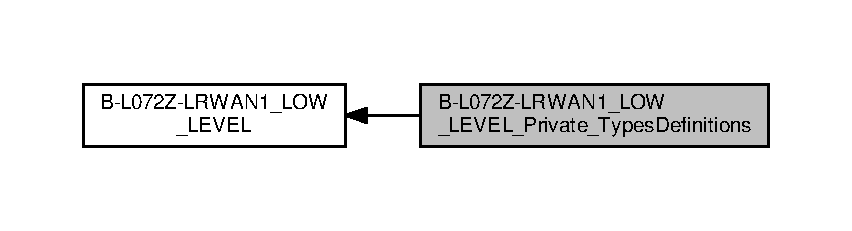
\includegraphics[width=350pt]{group__B-L072Z-LRWAN1__LOW__LEVEL__Private__TypesDefinitions}
\end{center}
\end{figure}

\hypertarget{group__B-L072Z-LRWAN1__LOW__LEVEL__Private__Defines}{}\section{B-\/\+L072\+Z-\/\+L\+R\+W\+A\+N1\+\_\+\+L\+O\+W\+\_\+\+L\+E\+V\+E\+L\+\_\+\+Private\+\_\+\+Defines}
\label{group__B-L072Z-LRWAN1__LOW__LEVEL__Private__Defines}\index{B-\/\+L072\+Z-\/\+L\+R\+W\+A\+N1\+\_\+\+L\+O\+W\+\_\+\+L\+E\+V\+E\+L\+\_\+\+Private\+\_\+\+Defines@{B-\/\+L072\+Z-\/\+L\+R\+W\+A\+N1\+\_\+\+L\+O\+W\+\_\+\+L\+E\+V\+E\+L\+\_\+\+Private\+\_\+\+Defines}}
Collaboration diagram for B-\/\+L072\+Z-\/\+L\+R\+W\+A\+N1\+\_\+\+L\+O\+W\+\_\+\+L\+E\+V\+E\+L\+\_\+\+Private\+\_\+\+Defines\+:
\nopagebreak
\begin{figure}[H]
\begin{center}
\leavevmode
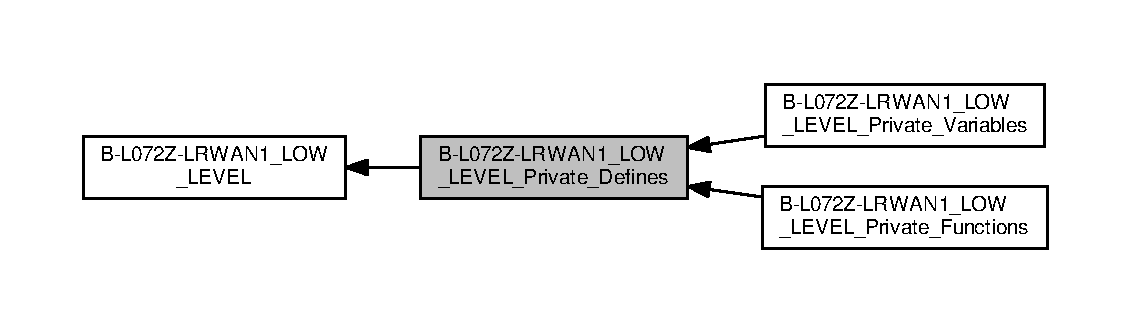
\includegraphics[width=350pt]{group__B-L072Z-LRWAN1__LOW__LEVEL__Private__Defines}
\end{center}
\end{figure}
\subsection*{Modules}
\begin{DoxyCompactItemize}
\item 
\hyperlink{group__B-L072Z-LRWAN1__LOW__LEVEL__Private__Variables}{B-\/\+L072\+Z-\/\+L\+R\+W\+A\+N1\+\_\+\+L\+O\+W\+\_\+\+L\+E\+V\+E\+L\+\_\+\+Private\+\_\+\+Variables}
\item 
\hyperlink{group__B-L072Z-LRWAN1__LOW__LEVEL__Private__Functions}{B-\/\+L072\+Z-\/\+L\+R\+W\+A\+N1\+\_\+\+L\+O\+W\+\_\+\+L\+E\+V\+E\+L\+\_\+\+Private\+\_\+\+Functions}
\end{DoxyCompactItemize}
\subsection*{Macros}
\begin{DoxyCompactItemize}
\item 
\#define \hyperlink{group__B-L072Z-LRWAN1__LOW__LEVEL__Private__Defines_gaf5f53a499afef1aaa3850de7086a11a5}{\+\_\+\+\_\+\+B\+\_\+\+L072\+Z\+\_\+\+L\+R\+W\+A\+N1\+\_\+\+B\+S\+P\+\_\+\+V\+E\+R\+S\+I\+O\+N\+\_\+\+M\+A\+IN}~(0x01)
\begin{DoxyCompactList}\small\item\em 32\+L082\+M\+LM D\+I\+S\+CO B\+SP Driver version number V1.\+0.\+0 \end{DoxyCompactList}\item 
\#define \hyperlink{group__B-L072Z-LRWAN1__LOW__LEVEL__Private__Defines_ga682147e46afbdf8d1002615e3ff7ad4a}{\+\_\+\+\_\+\+B\+\_\+\+L072\+Z\+\_\+\+L\+R\+W\+A\+N1\+\_\+\+B\+S\+P\+\_\+\+V\+E\+R\+S\+I\+O\+N\+\_\+\+S\+U\+B1}~(0x00)
\item 
\#define \hyperlink{group__B-L072Z-LRWAN1__LOW__LEVEL__Private__Defines_gaf0b4c3a1aa8fd40d74fc5fe1c845059e}{\+\_\+\+\_\+\+B\+\_\+\+L072\+Z\+\_\+\+L\+R\+W\+A\+N1\+\_\+\+B\+S\+P\+\_\+\+V\+E\+R\+S\+I\+O\+N\+\_\+\+S\+U\+B2}~(0x00)
\item 
\#define \hyperlink{group__B-L072Z-LRWAN1__LOW__LEVEL__Private__Defines_ga1c5543dd393ec382e3cee4c35b86c9cd}{\+\_\+\+\_\+\+B\+\_\+\+L072\+Z\+\_\+\+L\+R\+W\+A\+N1\+\_\+\+B\+S\+P\+\_\+\+V\+E\+R\+S\+I\+O\+N\+\_\+\+RC}~(0x00)
\item 
\#define \hyperlink{group__B-L072Z-LRWAN1__LOW__LEVEL__Private__Defines_ga62f40f0f53b1c1d1f0aaaa7fb0b63d5f}{\+\_\+\+\_\+\+B\+\_\+\+L072\+Z\+\_\+\+L\+R\+W\+A\+N1\+\_\+\+B\+S\+P\+\_\+\+V\+E\+R\+S\+I\+ON}
\end{DoxyCompactItemize}
\subsection*{Functions}
\begin{DoxyCompactItemize}
\item 
uint32\+\_\+t \hyperlink{group__B-L072Z-LRWAN1__LOW__LEVEL__Private__Defines_ga65d13608f7010a8068614154cb142cd6}{B\+S\+P\+\_\+\+Get\+Version} (void)
\begin{DoxyCompactList}\small\item\em This method returns the B-\/\+L072\+Z-\/\+L\+R\+W\+A\+N1 B\+SP Driver revision. \end{DoxyCompactList}\item 
void \hyperlink{group__B-L072Z-LRWAN1__LOW__LEVEL__Private__Defines_gab58a4f16a476a53653c5c400e3bed158}{B\+S\+P\+\_\+\+L\+E\+D\+\_\+\+Init} (\hyperlink{group__B-L072Z-LRWAN1__LOW__LEVEL__Exported__Types_gaa059704b7ca945eb9c1e7f2c3d03fecd}{Led\+\_\+\+Type\+Def} Led)
\begin{DoxyCompactList}\small\item\em Configures L\+ED G\+P\+IO. \end{DoxyCompactList}\item 
void \hyperlink{group__B-L072Z-LRWAN1__LOW__LEVEL__Private__Defines_gaee9c16b16384834c69efabf58f423d6f}{B\+S\+P\+\_\+\+L\+E\+D\+\_\+\+On} (\hyperlink{group__B-L072Z-LRWAN1__LOW__LEVEL__Exported__Types_gaa059704b7ca945eb9c1e7f2c3d03fecd}{Led\+\_\+\+Type\+Def} Led)
\begin{DoxyCompactList}\small\item\em Turns selected L\+ED On. \end{DoxyCompactList}\item 
void \hyperlink{group__B-L072Z-LRWAN1__LOW__LEVEL__Private__Defines_gaef268680154ca15c45066d64d41f9467}{B\+S\+P\+\_\+\+L\+E\+D\+\_\+\+Off} (\hyperlink{group__B-L072Z-LRWAN1__LOW__LEVEL__Exported__Types_gaa059704b7ca945eb9c1e7f2c3d03fecd}{Led\+\_\+\+Type\+Def} Led)
\begin{DoxyCompactList}\small\item\em Turns selected L\+ED Off. \end{DoxyCompactList}\item 
void \hyperlink{group__B-L072Z-LRWAN1__LOW__LEVEL__Private__Defines_ga1b9eabba7d498f41d6f16587ec0f9732}{B\+S\+P\+\_\+\+L\+E\+D\+\_\+\+Toggle} (\hyperlink{group__B-L072Z-LRWAN1__LOW__LEVEL__Exported__Types_gaa059704b7ca945eb9c1e7f2c3d03fecd}{Led\+\_\+\+Type\+Def} Led)
\begin{DoxyCompactList}\small\item\em Toggles the selected L\+ED. \end{DoxyCompactList}\item 
void \hyperlink{group__B-L072Z-LRWAN1__LOW__LEVEL__Private__Defines_gad31c8db50a71c1f6dbfe132d72ba0bc6}{B\+S\+P\+\_\+\+P\+B\+\_\+\+Init} (\hyperlink{group__B-L072Z-LRWAN1__LOW__LEVEL__Exported__Types_ga643816dfbad5c734fc25a29ce8d35bb1}{Button\+\_\+\+Type\+Def} Button, \hyperlink{group__B-L072Z-LRWAN1__LOW__LEVEL__Exported__Types_ga48825b7c7d851c440ef8e808fd9d8f0a}{Button\+Mode\+\_\+\+Type\+Def} Button\+Mode)
\begin{DoxyCompactList}\small\item\em Configures Button G\+P\+IO and E\+X\+TI Line. \end{DoxyCompactList}\item 
uint32\+\_\+t \hyperlink{group__B-L072Z-LRWAN1__LOW__LEVEL__Private__Defines_ga8f0978b6cffda9c67266ddfdb3a0abf7}{B\+S\+P\+\_\+\+P\+B\+\_\+\+Get\+State} (\hyperlink{group__B-L072Z-LRWAN1__LOW__LEVEL__Exported__Types_ga643816dfbad5c734fc25a29ce8d35bb1}{Button\+\_\+\+Type\+Def} Button)
\begin{DoxyCompactList}\small\item\em Returns the selected Button state. \end{DoxyCompactList}\end{DoxyCompactItemize}


\subsection{Detailed Description}


\subsection{Macro Definition Documentation}
\mbox{\Hypertarget{group__B-L072Z-LRWAN1__LOW__LEVEL__Private__Defines_ga62f40f0f53b1c1d1f0aaaa7fb0b63d5f}\label{group__B-L072Z-LRWAN1__LOW__LEVEL__Private__Defines_ga62f40f0f53b1c1d1f0aaaa7fb0b63d5f}} 
\index{B-\/\+L072\+Z-\/\+L\+R\+W\+A\+N1\+\_\+\+L\+O\+W\+\_\+\+L\+E\+V\+E\+L\+\_\+\+Private\+\_\+\+Defines@{B-\/\+L072\+Z-\/\+L\+R\+W\+A\+N1\+\_\+\+L\+O\+W\+\_\+\+L\+E\+V\+E\+L\+\_\+\+Private\+\_\+\+Defines}!\+\_\+\+\_\+\+B\+\_\+\+L072\+Z\+\_\+\+L\+R\+W\+A\+N1\+\_\+\+B\+S\+P\+\_\+\+V\+E\+R\+S\+I\+ON@{\+\_\+\+\_\+\+B\+\_\+\+L072\+Z\+\_\+\+L\+R\+W\+A\+N1\+\_\+\+B\+S\+P\+\_\+\+V\+E\+R\+S\+I\+ON}}
\index{\+\_\+\+\_\+\+B\+\_\+\+L072\+Z\+\_\+\+L\+R\+W\+A\+N1\+\_\+\+B\+S\+P\+\_\+\+V\+E\+R\+S\+I\+ON@{\+\_\+\+\_\+\+B\+\_\+\+L072\+Z\+\_\+\+L\+R\+W\+A\+N1\+\_\+\+B\+S\+P\+\_\+\+V\+E\+R\+S\+I\+ON}!B-\/\+L072\+Z-\/\+L\+R\+W\+A\+N1\+\_\+\+L\+O\+W\+\_\+\+L\+E\+V\+E\+L\+\_\+\+Private\+\_\+\+Defines@{B-\/\+L072\+Z-\/\+L\+R\+W\+A\+N1\+\_\+\+L\+O\+W\+\_\+\+L\+E\+V\+E\+L\+\_\+\+Private\+\_\+\+Defines}}
\subsubsection{\texorpdfstring{\+\_\+\+\_\+\+B\+\_\+\+L072\+Z\+\_\+\+L\+R\+W\+A\+N1\+\_\+\+B\+S\+P\+\_\+\+V\+E\+R\+S\+I\+ON}{\_\_B\_L072Z\_LRWAN1\_BSP\_VERSION}}
{\footnotesize\ttfamily \#define \+\_\+\+\_\+\+B\+\_\+\+L072\+Z\+\_\+\+L\+R\+W\+A\+N1\+\_\+\+B\+S\+P\+\_\+\+V\+E\+R\+S\+I\+ON}

{\bfseries Value\+:}
\begin{DoxyCode}
((\hyperlink{group__B-L072Z-LRWAN1__LOW__LEVEL__Private__Defines_gaf5f53a499afef1aaa3850de7086a11a5}{\_\_B\_L072Z\_LRWAN1\_BSP\_VERSION\_MAIN} << 24)\(\backslash\)
                                             |(\hyperlink{group__B-L072Z-LRWAN1__LOW__LEVEL__Private__Defines_ga682147e46afbdf8d1002615e3ff7ad4a}{\_\_B\_L072Z\_LRWAN1\_BSP\_VERSION\_SUB1}
       << 16)\(\backslash\)
                                             |(\hyperlink{group__B-L072Z-LRWAN1__LOW__LEVEL__Private__Defines_gaf0b4c3a1aa8fd40d74fc5fe1c845059e}{\_\_B\_L072Z\_LRWAN1\_BSP\_VERSION\_SUB2}
       << 8 )\(\backslash\)
                                             |(\hyperlink{group__B-L072Z-LRWAN1__LOW__LEVEL__Private__Defines_ga1c5543dd393ec382e3cee4c35b86c9cd}{\_\_B\_L072Z\_LRWAN1\_BSP\_VERSION\_RC}
      ))
\end{DoxyCode}
\mbox{\Hypertarget{group__B-L072Z-LRWAN1__LOW__LEVEL__Private__Defines_gaf5f53a499afef1aaa3850de7086a11a5}\label{group__B-L072Z-LRWAN1__LOW__LEVEL__Private__Defines_gaf5f53a499afef1aaa3850de7086a11a5}} 
\index{B-\/\+L072\+Z-\/\+L\+R\+W\+A\+N1\+\_\+\+L\+O\+W\+\_\+\+L\+E\+V\+E\+L\+\_\+\+Private\+\_\+\+Defines@{B-\/\+L072\+Z-\/\+L\+R\+W\+A\+N1\+\_\+\+L\+O\+W\+\_\+\+L\+E\+V\+E\+L\+\_\+\+Private\+\_\+\+Defines}!\+\_\+\+\_\+\+B\+\_\+\+L072\+Z\+\_\+\+L\+R\+W\+A\+N1\+\_\+\+B\+S\+P\+\_\+\+V\+E\+R\+S\+I\+O\+N\+\_\+\+M\+A\+IN@{\+\_\+\+\_\+\+B\+\_\+\+L072\+Z\+\_\+\+L\+R\+W\+A\+N1\+\_\+\+B\+S\+P\+\_\+\+V\+E\+R\+S\+I\+O\+N\+\_\+\+M\+A\+IN}}
\index{\+\_\+\+\_\+\+B\+\_\+\+L072\+Z\+\_\+\+L\+R\+W\+A\+N1\+\_\+\+B\+S\+P\+\_\+\+V\+E\+R\+S\+I\+O\+N\+\_\+\+M\+A\+IN@{\+\_\+\+\_\+\+B\+\_\+\+L072\+Z\+\_\+\+L\+R\+W\+A\+N1\+\_\+\+B\+S\+P\+\_\+\+V\+E\+R\+S\+I\+O\+N\+\_\+\+M\+A\+IN}!B-\/\+L072\+Z-\/\+L\+R\+W\+A\+N1\+\_\+\+L\+O\+W\+\_\+\+L\+E\+V\+E\+L\+\_\+\+Private\+\_\+\+Defines@{B-\/\+L072\+Z-\/\+L\+R\+W\+A\+N1\+\_\+\+L\+O\+W\+\_\+\+L\+E\+V\+E\+L\+\_\+\+Private\+\_\+\+Defines}}
\subsubsection{\texorpdfstring{\+\_\+\+\_\+\+B\+\_\+\+L072\+Z\+\_\+\+L\+R\+W\+A\+N1\+\_\+\+B\+S\+P\+\_\+\+V\+E\+R\+S\+I\+O\+N\+\_\+\+M\+A\+IN}{\_\_B\_L072Z\_LRWAN1\_BSP\_VERSION\_MAIN}}
{\footnotesize\ttfamily \#define \+\_\+\+\_\+\+B\+\_\+\+L072\+Z\+\_\+\+L\+R\+W\+A\+N1\+\_\+\+B\+S\+P\+\_\+\+V\+E\+R\+S\+I\+O\+N\+\_\+\+M\+A\+IN~(0x01)}



32\+L082\+M\+LM D\+I\+S\+CO B\+SP Driver version number V1.\+0.\+0 

\mbox{[}31\+:24\mbox{]} main version \mbox{\Hypertarget{group__B-L072Z-LRWAN1__LOW__LEVEL__Private__Defines_ga1c5543dd393ec382e3cee4c35b86c9cd}\label{group__B-L072Z-LRWAN1__LOW__LEVEL__Private__Defines_ga1c5543dd393ec382e3cee4c35b86c9cd}} 
\index{B-\/\+L072\+Z-\/\+L\+R\+W\+A\+N1\+\_\+\+L\+O\+W\+\_\+\+L\+E\+V\+E\+L\+\_\+\+Private\+\_\+\+Defines@{B-\/\+L072\+Z-\/\+L\+R\+W\+A\+N1\+\_\+\+L\+O\+W\+\_\+\+L\+E\+V\+E\+L\+\_\+\+Private\+\_\+\+Defines}!\+\_\+\+\_\+\+B\+\_\+\+L072\+Z\+\_\+\+L\+R\+W\+A\+N1\+\_\+\+B\+S\+P\+\_\+\+V\+E\+R\+S\+I\+O\+N\+\_\+\+RC@{\+\_\+\+\_\+\+B\+\_\+\+L072\+Z\+\_\+\+L\+R\+W\+A\+N1\+\_\+\+B\+S\+P\+\_\+\+V\+E\+R\+S\+I\+O\+N\+\_\+\+RC}}
\index{\+\_\+\+\_\+\+B\+\_\+\+L072\+Z\+\_\+\+L\+R\+W\+A\+N1\+\_\+\+B\+S\+P\+\_\+\+V\+E\+R\+S\+I\+O\+N\+\_\+\+RC@{\+\_\+\+\_\+\+B\+\_\+\+L072\+Z\+\_\+\+L\+R\+W\+A\+N1\+\_\+\+B\+S\+P\+\_\+\+V\+E\+R\+S\+I\+O\+N\+\_\+\+RC}!B-\/\+L072\+Z-\/\+L\+R\+W\+A\+N1\+\_\+\+L\+O\+W\+\_\+\+L\+E\+V\+E\+L\+\_\+\+Private\+\_\+\+Defines@{B-\/\+L072\+Z-\/\+L\+R\+W\+A\+N1\+\_\+\+L\+O\+W\+\_\+\+L\+E\+V\+E\+L\+\_\+\+Private\+\_\+\+Defines}}
\subsubsection{\texorpdfstring{\+\_\+\+\_\+\+B\+\_\+\+L072\+Z\+\_\+\+L\+R\+W\+A\+N1\+\_\+\+B\+S\+P\+\_\+\+V\+E\+R\+S\+I\+O\+N\+\_\+\+RC}{\_\_B\_L072Z\_LRWAN1\_BSP\_VERSION\_RC}}
{\footnotesize\ttfamily \#define \+\_\+\+\_\+\+B\+\_\+\+L072\+Z\+\_\+\+L\+R\+W\+A\+N1\+\_\+\+B\+S\+P\+\_\+\+V\+E\+R\+S\+I\+O\+N\+\_\+\+RC~(0x00)}

\mbox{[}7\+:0\mbox{]} release candidate \mbox{\Hypertarget{group__B-L072Z-LRWAN1__LOW__LEVEL__Private__Defines_ga682147e46afbdf8d1002615e3ff7ad4a}\label{group__B-L072Z-LRWAN1__LOW__LEVEL__Private__Defines_ga682147e46afbdf8d1002615e3ff7ad4a}} 
\index{B-\/\+L072\+Z-\/\+L\+R\+W\+A\+N1\+\_\+\+L\+O\+W\+\_\+\+L\+E\+V\+E\+L\+\_\+\+Private\+\_\+\+Defines@{B-\/\+L072\+Z-\/\+L\+R\+W\+A\+N1\+\_\+\+L\+O\+W\+\_\+\+L\+E\+V\+E\+L\+\_\+\+Private\+\_\+\+Defines}!\+\_\+\+\_\+\+B\+\_\+\+L072\+Z\+\_\+\+L\+R\+W\+A\+N1\+\_\+\+B\+S\+P\+\_\+\+V\+E\+R\+S\+I\+O\+N\+\_\+\+S\+U\+B1@{\+\_\+\+\_\+\+B\+\_\+\+L072\+Z\+\_\+\+L\+R\+W\+A\+N1\+\_\+\+B\+S\+P\+\_\+\+V\+E\+R\+S\+I\+O\+N\+\_\+\+S\+U\+B1}}
\index{\+\_\+\+\_\+\+B\+\_\+\+L072\+Z\+\_\+\+L\+R\+W\+A\+N1\+\_\+\+B\+S\+P\+\_\+\+V\+E\+R\+S\+I\+O\+N\+\_\+\+S\+U\+B1@{\+\_\+\+\_\+\+B\+\_\+\+L072\+Z\+\_\+\+L\+R\+W\+A\+N1\+\_\+\+B\+S\+P\+\_\+\+V\+E\+R\+S\+I\+O\+N\+\_\+\+S\+U\+B1}!B-\/\+L072\+Z-\/\+L\+R\+W\+A\+N1\+\_\+\+L\+O\+W\+\_\+\+L\+E\+V\+E\+L\+\_\+\+Private\+\_\+\+Defines@{B-\/\+L072\+Z-\/\+L\+R\+W\+A\+N1\+\_\+\+L\+O\+W\+\_\+\+L\+E\+V\+E\+L\+\_\+\+Private\+\_\+\+Defines}}
\subsubsection{\texorpdfstring{\+\_\+\+\_\+\+B\+\_\+\+L072\+Z\+\_\+\+L\+R\+W\+A\+N1\+\_\+\+B\+S\+P\+\_\+\+V\+E\+R\+S\+I\+O\+N\+\_\+\+S\+U\+B1}{\_\_B\_L072Z\_LRWAN1\_BSP\_VERSION\_SUB1}}
{\footnotesize\ttfamily \#define \+\_\+\+\_\+\+B\+\_\+\+L072\+Z\+\_\+\+L\+R\+W\+A\+N1\+\_\+\+B\+S\+P\+\_\+\+V\+E\+R\+S\+I\+O\+N\+\_\+\+S\+U\+B1~(0x00)}

\mbox{[}23\+:16\mbox{]} sub1 version \mbox{\Hypertarget{group__B-L072Z-LRWAN1__LOW__LEVEL__Private__Defines_gaf0b4c3a1aa8fd40d74fc5fe1c845059e}\label{group__B-L072Z-LRWAN1__LOW__LEVEL__Private__Defines_gaf0b4c3a1aa8fd40d74fc5fe1c845059e}} 
\index{B-\/\+L072\+Z-\/\+L\+R\+W\+A\+N1\+\_\+\+L\+O\+W\+\_\+\+L\+E\+V\+E\+L\+\_\+\+Private\+\_\+\+Defines@{B-\/\+L072\+Z-\/\+L\+R\+W\+A\+N1\+\_\+\+L\+O\+W\+\_\+\+L\+E\+V\+E\+L\+\_\+\+Private\+\_\+\+Defines}!\+\_\+\+\_\+\+B\+\_\+\+L072\+Z\+\_\+\+L\+R\+W\+A\+N1\+\_\+\+B\+S\+P\+\_\+\+V\+E\+R\+S\+I\+O\+N\+\_\+\+S\+U\+B2@{\+\_\+\+\_\+\+B\+\_\+\+L072\+Z\+\_\+\+L\+R\+W\+A\+N1\+\_\+\+B\+S\+P\+\_\+\+V\+E\+R\+S\+I\+O\+N\+\_\+\+S\+U\+B2}}
\index{\+\_\+\+\_\+\+B\+\_\+\+L072\+Z\+\_\+\+L\+R\+W\+A\+N1\+\_\+\+B\+S\+P\+\_\+\+V\+E\+R\+S\+I\+O\+N\+\_\+\+S\+U\+B2@{\+\_\+\+\_\+\+B\+\_\+\+L072\+Z\+\_\+\+L\+R\+W\+A\+N1\+\_\+\+B\+S\+P\+\_\+\+V\+E\+R\+S\+I\+O\+N\+\_\+\+S\+U\+B2}!B-\/\+L072\+Z-\/\+L\+R\+W\+A\+N1\+\_\+\+L\+O\+W\+\_\+\+L\+E\+V\+E\+L\+\_\+\+Private\+\_\+\+Defines@{B-\/\+L072\+Z-\/\+L\+R\+W\+A\+N1\+\_\+\+L\+O\+W\+\_\+\+L\+E\+V\+E\+L\+\_\+\+Private\+\_\+\+Defines}}
\subsubsection{\texorpdfstring{\+\_\+\+\_\+\+B\+\_\+\+L072\+Z\+\_\+\+L\+R\+W\+A\+N1\+\_\+\+B\+S\+P\+\_\+\+V\+E\+R\+S\+I\+O\+N\+\_\+\+S\+U\+B2}{\_\_B\_L072Z\_LRWAN1\_BSP\_VERSION\_SUB2}}
{\footnotesize\ttfamily \#define \+\_\+\+\_\+\+B\+\_\+\+L072\+Z\+\_\+\+L\+R\+W\+A\+N1\+\_\+\+B\+S\+P\+\_\+\+V\+E\+R\+S\+I\+O\+N\+\_\+\+S\+U\+B2~(0x00)}

\mbox{[}15\+:8\mbox{]} sub2 version 

\subsection{Function Documentation}
\mbox{\Hypertarget{group__B-L072Z-LRWAN1__LOW__LEVEL__Private__Defines_ga65d13608f7010a8068614154cb142cd6}\label{group__B-L072Z-LRWAN1__LOW__LEVEL__Private__Defines_ga65d13608f7010a8068614154cb142cd6}} 
\index{B-\/\+L072\+Z-\/\+L\+R\+W\+A\+N1\+\_\+\+L\+O\+W\+\_\+\+L\+E\+V\+E\+L\+\_\+\+Private\+\_\+\+Defines@{B-\/\+L072\+Z-\/\+L\+R\+W\+A\+N1\+\_\+\+L\+O\+W\+\_\+\+L\+E\+V\+E\+L\+\_\+\+Private\+\_\+\+Defines}!B\+S\+P\+\_\+\+Get\+Version@{B\+S\+P\+\_\+\+Get\+Version}}
\index{B\+S\+P\+\_\+\+Get\+Version@{B\+S\+P\+\_\+\+Get\+Version}!B-\/\+L072\+Z-\/\+L\+R\+W\+A\+N1\+\_\+\+L\+O\+W\+\_\+\+L\+E\+V\+E\+L\+\_\+\+Private\+\_\+\+Defines@{B-\/\+L072\+Z-\/\+L\+R\+W\+A\+N1\+\_\+\+L\+O\+W\+\_\+\+L\+E\+V\+E\+L\+\_\+\+Private\+\_\+\+Defines}}
\subsubsection{\texorpdfstring{B\+S\+P\+\_\+\+Get\+Version()}{BSP\_GetVersion()}}
{\footnotesize\ttfamily uint32\+\_\+t B\+S\+P\+\_\+\+Get\+Version (\begin{DoxyParamCaption}\item[{void}]{ }\end{DoxyParamCaption})}



This method returns the B-\/\+L072\+Z-\/\+L\+R\+W\+A\+N1 B\+SP Driver revision. 


\begin{DoxyParams}{Parameters}
{\em None} & \\
\hline
\end{DoxyParams}

\begin{DoxyRetVals}{Return values}
{\em version} & \+: 0x\+X\+Y\+ZR (8bits for each decimal, R for RC) \\
\hline
\end{DoxyRetVals}
\mbox{\Hypertarget{group__B-L072Z-LRWAN1__LOW__LEVEL__Private__Defines_gab58a4f16a476a53653c5c400e3bed158}\label{group__B-L072Z-LRWAN1__LOW__LEVEL__Private__Defines_gab58a4f16a476a53653c5c400e3bed158}} 
\index{B-\/\+L072\+Z-\/\+L\+R\+W\+A\+N1\+\_\+\+L\+O\+W\+\_\+\+L\+E\+V\+E\+L\+\_\+\+Private\+\_\+\+Defines@{B-\/\+L072\+Z-\/\+L\+R\+W\+A\+N1\+\_\+\+L\+O\+W\+\_\+\+L\+E\+V\+E\+L\+\_\+\+Private\+\_\+\+Defines}!B\+S\+P\+\_\+\+L\+E\+D\+\_\+\+Init@{B\+S\+P\+\_\+\+L\+E\+D\+\_\+\+Init}}
\index{B\+S\+P\+\_\+\+L\+E\+D\+\_\+\+Init@{B\+S\+P\+\_\+\+L\+E\+D\+\_\+\+Init}!B-\/\+L072\+Z-\/\+L\+R\+W\+A\+N1\+\_\+\+L\+O\+W\+\_\+\+L\+E\+V\+E\+L\+\_\+\+Private\+\_\+\+Defines@{B-\/\+L072\+Z-\/\+L\+R\+W\+A\+N1\+\_\+\+L\+O\+W\+\_\+\+L\+E\+V\+E\+L\+\_\+\+Private\+\_\+\+Defines}}
\subsubsection{\texorpdfstring{B\+S\+P\+\_\+\+L\+E\+D\+\_\+\+Init()}{BSP\_LED\_Init()}}
{\footnotesize\ttfamily void B\+S\+P\+\_\+\+L\+E\+D\+\_\+\+Init (\begin{DoxyParamCaption}\item[{\hyperlink{group__B-L072Z-LRWAN1__LOW__LEVEL__Exported__Types_gaa059704b7ca945eb9c1e7f2c3d03fecd}{Led\+\_\+\+Type\+Def}}]{Led }\end{DoxyParamCaption})}



Configures L\+ED G\+P\+IO. 


\begin{DoxyParams}{Parameters}
{\em Led} & Specifies the Led to be configured. This parameter can be one of following parameters\+: \begin{DoxyItemize}
\item L\+E\+D2 \end{DoxyItemize}
\\
\hline
\end{DoxyParams}

\begin{DoxyRetVals}{Return values}
{\em None} & \\
\hline
\end{DoxyRetVals}
\mbox{\Hypertarget{group__B-L072Z-LRWAN1__LOW__LEVEL__Private__Defines_gaef268680154ca15c45066d64d41f9467}\label{group__B-L072Z-LRWAN1__LOW__LEVEL__Private__Defines_gaef268680154ca15c45066d64d41f9467}} 
\index{B-\/\+L072\+Z-\/\+L\+R\+W\+A\+N1\+\_\+\+L\+O\+W\+\_\+\+L\+E\+V\+E\+L\+\_\+\+Private\+\_\+\+Defines@{B-\/\+L072\+Z-\/\+L\+R\+W\+A\+N1\+\_\+\+L\+O\+W\+\_\+\+L\+E\+V\+E\+L\+\_\+\+Private\+\_\+\+Defines}!B\+S\+P\+\_\+\+L\+E\+D\+\_\+\+Off@{B\+S\+P\+\_\+\+L\+E\+D\+\_\+\+Off}}
\index{B\+S\+P\+\_\+\+L\+E\+D\+\_\+\+Off@{B\+S\+P\+\_\+\+L\+E\+D\+\_\+\+Off}!B-\/\+L072\+Z-\/\+L\+R\+W\+A\+N1\+\_\+\+L\+O\+W\+\_\+\+L\+E\+V\+E\+L\+\_\+\+Private\+\_\+\+Defines@{B-\/\+L072\+Z-\/\+L\+R\+W\+A\+N1\+\_\+\+L\+O\+W\+\_\+\+L\+E\+V\+E\+L\+\_\+\+Private\+\_\+\+Defines}}
\subsubsection{\texorpdfstring{B\+S\+P\+\_\+\+L\+E\+D\+\_\+\+Off()}{BSP\_LED\_Off()}}
{\footnotesize\ttfamily void B\+S\+P\+\_\+\+L\+E\+D\+\_\+\+Off (\begin{DoxyParamCaption}\item[{\hyperlink{group__B-L072Z-LRWAN1__LOW__LEVEL__Exported__Types_gaa059704b7ca945eb9c1e7f2c3d03fecd}{Led\+\_\+\+Type\+Def}}]{Led }\end{DoxyParamCaption})}



Turns selected L\+ED Off. 


\begin{DoxyParams}{Parameters}
{\em Led} & Specifies the Led to be set off. This parameter can be one of following parameters\+: \begin{DoxyItemize}
\item L\+E\+D2 \end{DoxyItemize}
\\
\hline
\end{DoxyParams}

\begin{DoxyRetVals}{Return values}
{\em None} & \\
\hline
\end{DoxyRetVals}
\mbox{\Hypertarget{group__B-L072Z-LRWAN1__LOW__LEVEL__Private__Defines_gaee9c16b16384834c69efabf58f423d6f}\label{group__B-L072Z-LRWAN1__LOW__LEVEL__Private__Defines_gaee9c16b16384834c69efabf58f423d6f}} 
\index{B-\/\+L072\+Z-\/\+L\+R\+W\+A\+N1\+\_\+\+L\+O\+W\+\_\+\+L\+E\+V\+E\+L\+\_\+\+Private\+\_\+\+Defines@{B-\/\+L072\+Z-\/\+L\+R\+W\+A\+N1\+\_\+\+L\+O\+W\+\_\+\+L\+E\+V\+E\+L\+\_\+\+Private\+\_\+\+Defines}!B\+S\+P\+\_\+\+L\+E\+D\+\_\+\+On@{B\+S\+P\+\_\+\+L\+E\+D\+\_\+\+On}}
\index{B\+S\+P\+\_\+\+L\+E\+D\+\_\+\+On@{B\+S\+P\+\_\+\+L\+E\+D\+\_\+\+On}!B-\/\+L072\+Z-\/\+L\+R\+W\+A\+N1\+\_\+\+L\+O\+W\+\_\+\+L\+E\+V\+E\+L\+\_\+\+Private\+\_\+\+Defines@{B-\/\+L072\+Z-\/\+L\+R\+W\+A\+N1\+\_\+\+L\+O\+W\+\_\+\+L\+E\+V\+E\+L\+\_\+\+Private\+\_\+\+Defines}}
\subsubsection{\texorpdfstring{B\+S\+P\+\_\+\+L\+E\+D\+\_\+\+On()}{BSP\_LED\_On()}}
{\footnotesize\ttfamily void B\+S\+P\+\_\+\+L\+E\+D\+\_\+\+On (\begin{DoxyParamCaption}\item[{\hyperlink{group__B-L072Z-LRWAN1__LOW__LEVEL__Exported__Types_gaa059704b7ca945eb9c1e7f2c3d03fecd}{Led\+\_\+\+Type\+Def}}]{Led }\end{DoxyParamCaption})}



Turns selected L\+ED On. 


\begin{DoxyParams}{Parameters}
{\em Led} & Specifies the Led to be set on. This parameter can be one of following parameters\+: \begin{DoxyItemize}
\item L\+E\+D2 \end{DoxyItemize}
\\
\hline
\end{DoxyParams}

\begin{DoxyRetVals}{Return values}
{\em None} & \\
\hline
\end{DoxyRetVals}
\mbox{\Hypertarget{group__B-L072Z-LRWAN1__LOW__LEVEL__Private__Defines_ga1b9eabba7d498f41d6f16587ec0f9732}\label{group__B-L072Z-LRWAN1__LOW__LEVEL__Private__Defines_ga1b9eabba7d498f41d6f16587ec0f9732}} 
\index{B-\/\+L072\+Z-\/\+L\+R\+W\+A\+N1\+\_\+\+L\+O\+W\+\_\+\+L\+E\+V\+E\+L\+\_\+\+Private\+\_\+\+Defines@{B-\/\+L072\+Z-\/\+L\+R\+W\+A\+N1\+\_\+\+L\+O\+W\+\_\+\+L\+E\+V\+E\+L\+\_\+\+Private\+\_\+\+Defines}!B\+S\+P\+\_\+\+L\+E\+D\+\_\+\+Toggle@{B\+S\+P\+\_\+\+L\+E\+D\+\_\+\+Toggle}}
\index{B\+S\+P\+\_\+\+L\+E\+D\+\_\+\+Toggle@{B\+S\+P\+\_\+\+L\+E\+D\+\_\+\+Toggle}!B-\/\+L072\+Z-\/\+L\+R\+W\+A\+N1\+\_\+\+L\+O\+W\+\_\+\+L\+E\+V\+E\+L\+\_\+\+Private\+\_\+\+Defines@{B-\/\+L072\+Z-\/\+L\+R\+W\+A\+N1\+\_\+\+L\+O\+W\+\_\+\+L\+E\+V\+E\+L\+\_\+\+Private\+\_\+\+Defines}}
\subsubsection{\texorpdfstring{B\+S\+P\+\_\+\+L\+E\+D\+\_\+\+Toggle()}{BSP\_LED\_Toggle()}}
{\footnotesize\ttfamily void B\+S\+P\+\_\+\+L\+E\+D\+\_\+\+Toggle (\begin{DoxyParamCaption}\item[{\hyperlink{group__B-L072Z-LRWAN1__LOW__LEVEL__Exported__Types_gaa059704b7ca945eb9c1e7f2c3d03fecd}{Led\+\_\+\+Type\+Def}}]{Led }\end{DoxyParamCaption})}



Toggles the selected L\+ED. 


\begin{DoxyParams}{Parameters}
{\em Led} & Specifies the Led to be toggled. This parameter can be one of following parameters\+: \begin{DoxyItemize}
\item L\+E\+D2 \end{DoxyItemize}
\\
\hline
\end{DoxyParams}

\begin{DoxyRetVals}{Return values}
{\em None} & \\
\hline
\end{DoxyRetVals}
\mbox{\Hypertarget{group__B-L072Z-LRWAN1__LOW__LEVEL__Private__Defines_ga8f0978b6cffda9c67266ddfdb3a0abf7}\label{group__B-L072Z-LRWAN1__LOW__LEVEL__Private__Defines_ga8f0978b6cffda9c67266ddfdb3a0abf7}} 
\index{B-\/\+L072\+Z-\/\+L\+R\+W\+A\+N1\+\_\+\+L\+O\+W\+\_\+\+L\+E\+V\+E\+L\+\_\+\+Private\+\_\+\+Defines@{B-\/\+L072\+Z-\/\+L\+R\+W\+A\+N1\+\_\+\+L\+O\+W\+\_\+\+L\+E\+V\+E\+L\+\_\+\+Private\+\_\+\+Defines}!B\+S\+P\+\_\+\+P\+B\+\_\+\+Get\+State@{B\+S\+P\+\_\+\+P\+B\+\_\+\+Get\+State}}
\index{B\+S\+P\+\_\+\+P\+B\+\_\+\+Get\+State@{B\+S\+P\+\_\+\+P\+B\+\_\+\+Get\+State}!B-\/\+L072\+Z-\/\+L\+R\+W\+A\+N1\+\_\+\+L\+O\+W\+\_\+\+L\+E\+V\+E\+L\+\_\+\+Private\+\_\+\+Defines@{B-\/\+L072\+Z-\/\+L\+R\+W\+A\+N1\+\_\+\+L\+O\+W\+\_\+\+L\+E\+V\+E\+L\+\_\+\+Private\+\_\+\+Defines}}
\subsubsection{\texorpdfstring{B\+S\+P\+\_\+\+P\+B\+\_\+\+Get\+State()}{BSP\_PB\_GetState()}}
{\footnotesize\ttfamily uint32\+\_\+t B\+S\+P\+\_\+\+P\+B\+\_\+\+Get\+State (\begin{DoxyParamCaption}\item[{\hyperlink{group__B-L072Z-LRWAN1__LOW__LEVEL__Exported__Types_ga643816dfbad5c734fc25a29ce8d35bb1}{Button\+\_\+\+Type\+Def}}]{Button }\end{DoxyParamCaption})}



Returns the selected Button state. 


\begin{DoxyParams}{Parameters}
{\em Button} & Specifies the Button to be checked. This parameter should be\+: B\+U\+T\+T\+O\+N\+\_\+\+K\+EY \\
\hline
\end{DoxyParams}

\begin{DoxyRetVals}{Return values}
{\em The} & Button G\+P\+IO pin value. \\
\hline
\end{DoxyRetVals}
\mbox{\Hypertarget{group__B-L072Z-LRWAN1__LOW__LEVEL__Private__Defines_gad31c8db50a71c1f6dbfe132d72ba0bc6}\label{group__B-L072Z-LRWAN1__LOW__LEVEL__Private__Defines_gad31c8db50a71c1f6dbfe132d72ba0bc6}} 
\index{B-\/\+L072\+Z-\/\+L\+R\+W\+A\+N1\+\_\+\+L\+O\+W\+\_\+\+L\+E\+V\+E\+L\+\_\+\+Private\+\_\+\+Defines@{B-\/\+L072\+Z-\/\+L\+R\+W\+A\+N1\+\_\+\+L\+O\+W\+\_\+\+L\+E\+V\+E\+L\+\_\+\+Private\+\_\+\+Defines}!B\+S\+P\+\_\+\+P\+B\+\_\+\+Init@{B\+S\+P\+\_\+\+P\+B\+\_\+\+Init}}
\index{B\+S\+P\+\_\+\+P\+B\+\_\+\+Init@{B\+S\+P\+\_\+\+P\+B\+\_\+\+Init}!B-\/\+L072\+Z-\/\+L\+R\+W\+A\+N1\+\_\+\+L\+O\+W\+\_\+\+L\+E\+V\+E\+L\+\_\+\+Private\+\_\+\+Defines@{B-\/\+L072\+Z-\/\+L\+R\+W\+A\+N1\+\_\+\+L\+O\+W\+\_\+\+L\+E\+V\+E\+L\+\_\+\+Private\+\_\+\+Defines}}
\subsubsection{\texorpdfstring{B\+S\+P\+\_\+\+P\+B\+\_\+\+Init()}{BSP\_PB\_Init()}}
{\footnotesize\ttfamily void B\+S\+P\+\_\+\+P\+B\+\_\+\+Init (\begin{DoxyParamCaption}\item[{\hyperlink{group__B-L072Z-LRWAN1__LOW__LEVEL__Exported__Types_ga643816dfbad5c734fc25a29ce8d35bb1}{Button\+\_\+\+Type\+Def}}]{Button,  }\item[{\hyperlink{group__B-L072Z-LRWAN1__LOW__LEVEL__Exported__Types_ga48825b7c7d851c440ef8e808fd9d8f0a}{Button\+Mode\+\_\+\+Type\+Def}}]{Button\+Mode }\end{DoxyParamCaption})}



Configures Button G\+P\+IO and E\+X\+TI Line. 


\begin{DoxyParams}{Parameters}
{\em Button} & Specifies the Button to be configured. This parameter should be\+: B\+U\+T\+T\+O\+N\+\_\+\+K\+EY \\
\hline
{\em Button\+Mode} & Specifies Button mode. This parameter can be one of following parameters\+: \begin{DoxyItemize}
\item B\+U\+T\+T\+O\+N\+\_\+\+M\+O\+D\+E\+\_\+\+G\+P\+IO\+: Button will be used as simple IO \item B\+U\+T\+T\+O\+N\+\_\+\+M\+O\+D\+E\+\_\+\+E\+X\+TI\+: Button will be connected to E\+X\+TI line with interrupt generation capability \end{DoxyItemize}
\\
\hline
\end{DoxyParams}

\begin{DoxyRetVals}{Return values}
{\em None} & \\
\hline
\end{DoxyRetVals}

\hypertarget{group__B-L072Z-LRWAN1__LOW__LEVEL__Private__Variables}{}\section{B-\/\+L072\+Z-\/\+L\+R\+W\+A\+N1\+\_\+\+L\+O\+W\+\_\+\+L\+E\+V\+E\+L\+\_\+\+Private\+\_\+\+Variables}
\label{group__B-L072Z-LRWAN1__LOW__LEVEL__Private__Variables}\index{B-\/\+L072\+Z-\/\+L\+R\+W\+A\+N1\+\_\+\+L\+O\+W\+\_\+\+L\+E\+V\+E\+L\+\_\+\+Private\+\_\+\+Variables@{B-\/\+L072\+Z-\/\+L\+R\+W\+A\+N1\+\_\+\+L\+O\+W\+\_\+\+L\+E\+V\+E\+L\+\_\+\+Private\+\_\+\+Variables}}
Collaboration diagram for B-\/\+L072\+Z-\/\+L\+R\+W\+A\+N1\+\_\+\+L\+O\+W\+\_\+\+L\+E\+V\+E\+L\+\_\+\+Private\+\_\+\+Variables\+:
\nopagebreak
\begin{figure}[H]
\begin{center}
\leavevmode
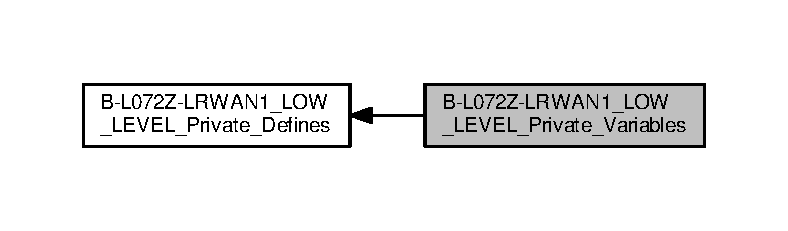
\includegraphics[width=350pt]{group__B-L072Z-LRWAN1__LOW__LEVEL__Private__Variables}
\end{center}
\end{figure}
\subsection*{Variables}
\begin{DoxyCompactItemize}
\item 
G\+P\+I\+O\+\_\+\+Type\+Def $\ast$ \hyperlink{group__B-L072Z-LRWAN1__LOW__LEVEL__Private__Variables_ga1127c0cf12e4ec7a66f2a64cd7407218}{L\+E\+D\+\_\+\+P\+O\+RT} \mbox{[}\hyperlink{group__B-L072Z-LRWAN1__LOW__LEVEL__LED_gab4be2480bf7d44d52aab1190a65a733c}{L\+E\+Dn}\mbox{]} = \{\hyperlink{group__B-L072Z-LRWAN1__LOW__LEVEL__LED_ga5d97443b4011e40e47164445dc1adde0}{L\+E\+D1\+\_\+\+G\+P\+I\+O\+\_\+\+P\+O\+RT}, \hyperlink{group__B-L072Z-LRWAN1__LOW__LEVEL__LED_gaf88822ae4b79d37c7735ce1160b59f68}{L\+E\+D2\+\_\+\+G\+P\+I\+O\+\_\+\+P\+O\+RT}, \hyperlink{group__B-L072Z-LRWAN1__LOW__LEVEL__LED_ga050f4b3a1f402476f9541dfe975d2143}{L\+E\+D3\+\_\+\+G\+P\+I\+O\+\_\+\+P\+O\+RT}, \hyperlink{group__B-L072Z-LRWAN1__LOW__LEVEL__LED_ga6b6f3eb4d23b770de265803afbc2b61b}{L\+E\+D4\+\_\+\+G\+P\+I\+O\+\_\+\+P\+O\+RT}\}
\item 
const uint16\+\_\+t \hyperlink{group__B-L072Z-LRWAN1__LOW__LEVEL__Private__Variables_ga51722a2d3aff3970f123a94ac62b908f}{L\+E\+D\+\_\+\+P\+IN} \mbox{[}\hyperlink{group__B-L072Z-LRWAN1__LOW__LEVEL__LED_gab4be2480bf7d44d52aab1190a65a733c}{L\+E\+Dn}\mbox{]} = \{\hyperlink{group__B-L072Z-LRWAN1__LOW__LEVEL__LED_ga318aa17e5d40e2132d2c7f6269ce7f51}{L\+E\+D1\+\_\+\+P\+IN}, \hyperlink{group__B-L072Z-LRWAN1__LOW__LEVEL__LED_gaf6f84078113b55354d20585131b386f7}{L\+E\+D2\+\_\+\+P\+IN},\hyperlink{group__B-L072Z-LRWAN1__LOW__LEVEL__LED_ga4cb3ff938bcabb01494ce529ae55a542}{L\+E\+D3\+\_\+\+P\+IN}, \hyperlink{group__B-L072Z-LRWAN1__LOW__LEVEL__LED_gaae684bb3d2f940637ccbc2adeb0e134d}{L\+E\+D4\+\_\+\+P\+IN}\}
\item 
G\+P\+I\+O\+\_\+\+Type\+Def $\ast$ \hyperlink{group__B-L072Z-LRWAN1__LOW__LEVEL__Private__Variables_gad63ed42b4071e78f80f7462227da4f35}{B\+U\+T\+T\+O\+N\+\_\+\+P\+O\+RT} \mbox{[}\hyperlink{group__B-L072Z-LRWAN1__LOW__LEVEL__BUTTON_ga43d47e509ada64329393005c3be15d64}{B\+U\+T\+T\+O\+Nn}\mbox{]} = \{\hyperlink{group__B-L072Z-LRWAN1__LOW__LEVEL__BUTTON_ga98680733a6992dacef531bfd0c23031c}{K\+E\+Y\+\_\+\+B\+U\+T\+T\+O\+N\+\_\+\+G\+P\+I\+O\+\_\+\+P\+O\+RT} \}
\item 
const uint16\+\_\+t \hyperlink{group__B-L072Z-LRWAN1__LOW__LEVEL__Private__Variables_gadf78f2d71408a01f8d30929c2d2da82b}{B\+U\+T\+T\+O\+N\+\_\+\+P\+IN} \mbox{[}\hyperlink{group__B-L072Z-LRWAN1__LOW__LEVEL__BUTTON_ga43d47e509ada64329393005c3be15d64}{B\+U\+T\+T\+O\+Nn}\mbox{]} = \{\hyperlink{group__B-L072Z-LRWAN1__LOW__LEVEL__BUTTON_ga5c260a4b4e26836dc3a9b6f15d317421}{K\+E\+Y\+\_\+\+B\+U\+T\+T\+O\+N\+\_\+\+P\+IN} \}
\item 
const uint8\+\_\+t \hyperlink{group__B-L072Z-LRWAN1__LOW__LEVEL__Private__Variables_ga13c3e27c584df9fccc4697dd535ea1cd}{B\+U\+T\+T\+O\+N\+\_\+\+I\+R\+Qn} \mbox{[}\hyperlink{group__B-L072Z-LRWAN1__LOW__LEVEL__BUTTON_ga43d47e509ada64329393005c3be15d64}{B\+U\+T\+T\+O\+Nn}\mbox{]} = \{\hyperlink{group__B-L072Z-LRWAN1__LOW__LEVEL__BUTTON_gaeb5bffe8281b0754675cfdfb2847e82d}{K\+E\+Y\+\_\+\+B\+U\+T\+T\+O\+N\+\_\+\+E\+X\+T\+I\+\_\+\+I\+R\+Qn} \}
\end{DoxyCompactItemize}


\subsection{Detailed Description}


\subsection{Variable Documentation}
\mbox{\Hypertarget{group__B-L072Z-LRWAN1__LOW__LEVEL__Private__Variables_ga13c3e27c584df9fccc4697dd535ea1cd}\label{group__B-L072Z-LRWAN1__LOW__LEVEL__Private__Variables_ga13c3e27c584df9fccc4697dd535ea1cd}} 
\index{B-\/\+L072\+Z-\/\+L\+R\+W\+A\+N1\+\_\+\+L\+O\+W\+\_\+\+L\+E\+V\+E\+L\+\_\+\+Private\+\_\+\+Variables@{B-\/\+L072\+Z-\/\+L\+R\+W\+A\+N1\+\_\+\+L\+O\+W\+\_\+\+L\+E\+V\+E\+L\+\_\+\+Private\+\_\+\+Variables}!B\+U\+T\+T\+O\+N\+\_\+\+I\+R\+Qn@{B\+U\+T\+T\+O\+N\+\_\+\+I\+R\+Qn}}
\index{B\+U\+T\+T\+O\+N\+\_\+\+I\+R\+Qn@{B\+U\+T\+T\+O\+N\+\_\+\+I\+R\+Qn}!B-\/\+L072\+Z-\/\+L\+R\+W\+A\+N1\+\_\+\+L\+O\+W\+\_\+\+L\+E\+V\+E\+L\+\_\+\+Private\+\_\+\+Variables@{B-\/\+L072\+Z-\/\+L\+R\+W\+A\+N1\+\_\+\+L\+O\+W\+\_\+\+L\+E\+V\+E\+L\+\_\+\+Private\+\_\+\+Variables}}
\subsubsection{\texorpdfstring{B\+U\+T\+T\+O\+N\+\_\+\+I\+R\+Qn}{BUTTON\_IRQn}}
{\footnotesize\ttfamily const uint8\+\_\+t B\+U\+T\+T\+O\+N\+\_\+\+I\+R\+Qn\mbox{[}\hyperlink{group__B-L072Z-LRWAN1__LOW__LEVEL__BUTTON_ga43d47e509ada64329393005c3be15d64}{B\+U\+T\+T\+O\+Nn}\mbox{]} = \{\hyperlink{group__B-L072Z-LRWAN1__LOW__LEVEL__BUTTON_gaeb5bffe8281b0754675cfdfb2847e82d}{K\+E\+Y\+\_\+\+B\+U\+T\+T\+O\+N\+\_\+\+E\+X\+T\+I\+\_\+\+I\+R\+Qn} \}}

\mbox{\Hypertarget{group__B-L072Z-LRWAN1__LOW__LEVEL__Private__Variables_gadf78f2d71408a01f8d30929c2d2da82b}\label{group__B-L072Z-LRWAN1__LOW__LEVEL__Private__Variables_gadf78f2d71408a01f8d30929c2d2da82b}} 
\index{B-\/\+L072\+Z-\/\+L\+R\+W\+A\+N1\+\_\+\+L\+O\+W\+\_\+\+L\+E\+V\+E\+L\+\_\+\+Private\+\_\+\+Variables@{B-\/\+L072\+Z-\/\+L\+R\+W\+A\+N1\+\_\+\+L\+O\+W\+\_\+\+L\+E\+V\+E\+L\+\_\+\+Private\+\_\+\+Variables}!B\+U\+T\+T\+O\+N\+\_\+\+P\+IN@{B\+U\+T\+T\+O\+N\+\_\+\+P\+IN}}
\index{B\+U\+T\+T\+O\+N\+\_\+\+P\+IN@{B\+U\+T\+T\+O\+N\+\_\+\+P\+IN}!B-\/\+L072\+Z-\/\+L\+R\+W\+A\+N1\+\_\+\+L\+O\+W\+\_\+\+L\+E\+V\+E\+L\+\_\+\+Private\+\_\+\+Variables@{B-\/\+L072\+Z-\/\+L\+R\+W\+A\+N1\+\_\+\+L\+O\+W\+\_\+\+L\+E\+V\+E\+L\+\_\+\+Private\+\_\+\+Variables}}
\subsubsection{\texorpdfstring{B\+U\+T\+T\+O\+N\+\_\+\+P\+IN}{BUTTON\_PIN}}
{\footnotesize\ttfamily const uint16\+\_\+t B\+U\+T\+T\+O\+N\+\_\+\+P\+IN\mbox{[}\hyperlink{group__B-L072Z-LRWAN1__LOW__LEVEL__BUTTON_ga43d47e509ada64329393005c3be15d64}{B\+U\+T\+T\+O\+Nn}\mbox{]} = \{\hyperlink{group__B-L072Z-LRWAN1__LOW__LEVEL__BUTTON_ga5c260a4b4e26836dc3a9b6f15d317421}{K\+E\+Y\+\_\+\+B\+U\+T\+T\+O\+N\+\_\+\+P\+IN} \}}

\mbox{\Hypertarget{group__B-L072Z-LRWAN1__LOW__LEVEL__Private__Variables_gad63ed42b4071e78f80f7462227da4f35}\label{group__B-L072Z-LRWAN1__LOW__LEVEL__Private__Variables_gad63ed42b4071e78f80f7462227da4f35}} 
\index{B-\/\+L072\+Z-\/\+L\+R\+W\+A\+N1\+\_\+\+L\+O\+W\+\_\+\+L\+E\+V\+E\+L\+\_\+\+Private\+\_\+\+Variables@{B-\/\+L072\+Z-\/\+L\+R\+W\+A\+N1\+\_\+\+L\+O\+W\+\_\+\+L\+E\+V\+E\+L\+\_\+\+Private\+\_\+\+Variables}!B\+U\+T\+T\+O\+N\+\_\+\+P\+O\+RT@{B\+U\+T\+T\+O\+N\+\_\+\+P\+O\+RT}}
\index{B\+U\+T\+T\+O\+N\+\_\+\+P\+O\+RT@{B\+U\+T\+T\+O\+N\+\_\+\+P\+O\+RT}!B-\/\+L072\+Z-\/\+L\+R\+W\+A\+N1\+\_\+\+L\+O\+W\+\_\+\+L\+E\+V\+E\+L\+\_\+\+Private\+\_\+\+Variables@{B-\/\+L072\+Z-\/\+L\+R\+W\+A\+N1\+\_\+\+L\+O\+W\+\_\+\+L\+E\+V\+E\+L\+\_\+\+Private\+\_\+\+Variables}}
\subsubsection{\texorpdfstring{B\+U\+T\+T\+O\+N\+\_\+\+P\+O\+RT}{BUTTON\_PORT}}
{\footnotesize\ttfamily G\+P\+I\+O\+\_\+\+Type\+Def$\ast$ B\+U\+T\+T\+O\+N\+\_\+\+P\+O\+RT\mbox{[}\hyperlink{group__B-L072Z-LRWAN1__LOW__LEVEL__BUTTON_ga43d47e509ada64329393005c3be15d64}{B\+U\+T\+T\+O\+Nn}\mbox{]} = \{\hyperlink{group__B-L072Z-LRWAN1__LOW__LEVEL__BUTTON_ga98680733a6992dacef531bfd0c23031c}{K\+E\+Y\+\_\+\+B\+U\+T\+T\+O\+N\+\_\+\+G\+P\+I\+O\+\_\+\+P\+O\+RT} \}}

\mbox{\Hypertarget{group__B-L072Z-LRWAN1__LOW__LEVEL__Private__Variables_ga51722a2d3aff3970f123a94ac62b908f}\label{group__B-L072Z-LRWAN1__LOW__LEVEL__Private__Variables_ga51722a2d3aff3970f123a94ac62b908f}} 
\index{B-\/\+L072\+Z-\/\+L\+R\+W\+A\+N1\+\_\+\+L\+O\+W\+\_\+\+L\+E\+V\+E\+L\+\_\+\+Private\+\_\+\+Variables@{B-\/\+L072\+Z-\/\+L\+R\+W\+A\+N1\+\_\+\+L\+O\+W\+\_\+\+L\+E\+V\+E\+L\+\_\+\+Private\+\_\+\+Variables}!L\+E\+D\+\_\+\+P\+IN@{L\+E\+D\+\_\+\+P\+IN}}
\index{L\+E\+D\+\_\+\+P\+IN@{L\+E\+D\+\_\+\+P\+IN}!B-\/\+L072\+Z-\/\+L\+R\+W\+A\+N1\+\_\+\+L\+O\+W\+\_\+\+L\+E\+V\+E\+L\+\_\+\+Private\+\_\+\+Variables@{B-\/\+L072\+Z-\/\+L\+R\+W\+A\+N1\+\_\+\+L\+O\+W\+\_\+\+L\+E\+V\+E\+L\+\_\+\+Private\+\_\+\+Variables}}
\subsubsection{\texorpdfstring{L\+E\+D\+\_\+\+P\+IN}{LED\_PIN}}
{\footnotesize\ttfamily const uint16\+\_\+t L\+E\+D\+\_\+\+P\+IN\mbox{[}\hyperlink{group__B-L072Z-LRWAN1__LOW__LEVEL__LED_gab4be2480bf7d44d52aab1190a65a733c}{L\+E\+Dn}\mbox{]} = \{\hyperlink{group__B-L072Z-LRWAN1__LOW__LEVEL__LED_ga318aa17e5d40e2132d2c7f6269ce7f51}{L\+E\+D1\+\_\+\+P\+IN}, \hyperlink{group__B-L072Z-LRWAN1__LOW__LEVEL__LED_gaf6f84078113b55354d20585131b386f7}{L\+E\+D2\+\_\+\+P\+IN},\hyperlink{group__B-L072Z-LRWAN1__LOW__LEVEL__LED_ga4cb3ff938bcabb01494ce529ae55a542}{L\+E\+D3\+\_\+\+P\+IN}, \hyperlink{group__B-L072Z-LRWAN1__LOW__LEVEL__LED_gaae684bb3d2f940637ccbc2adeb0e134d}{L\+E\+D4\+\_\+\+P\+IN}\}}

\mbox{\Hypertarget{group__B-L072Z-LRWAN1__LOW__LEVEL__Private__Variables_ga1127c0cf12e4ec7a66f2a64cd7407218}\label{group__B-L072Z-LRWAN1__LOW__LEVEL__Private__Variables_ga1127c0cf12e4ec7a66f2a64cd7407218}} 
\index{B-\/\+L072\+Z-\/\+L\+R\+W\+A\+N1\+\_\+\+L\+O\+W\+\_\+\+L\+E\+V\+E\+L\+\_\+\+Private\+\_\+\+Variables@{B-\/\+L072\+Z-\/\+L\+R\+W\+A\+N1\+\_\+\+L\+O\+W\+\_\+\+L\+E\+V\+E\+L\+\_\+\+Private\+\_\+\+Variables}!L\+E\+D\+\_\+\+P\+O\+RT@{L\+E\+D\+\_\+\+P\+O\+RT}}
\index{L\+E\+D\+\_\+\+P\+O\+RT@{L\+E\+D\+\_\+\+P\+O\+RT}!B-\/\+L072\+Z-\/\+L\+R\+W\+A\+N1\+\_\+\+L\+O\+W\+\_\+\+L\+E\+V\+E\+L\+\_\+\+Private\+\_\+\+Variables@{B-\/\+L072\+Z-\/\+L\+R\+W\+A\+N1\+\_\+\+L\+O\+W\+\_\+\+L\+E\+V\+E\+L\+\_\+\+Private\+\_\+\+Variables}}
\subsubsection{\texorpdfstring{L\+E\+D\+\_\+\+P\+O\+RT}{LED\_PORT}}
{\footnotesize\ttfamily G\+P\+I\+O\+\_\+\+Type\+Def$\ast$ L\+E\+D\+\_\+\+P\+O\+RT\mbox{[}\hyperlink{group__B-L072Z-LRWAN1__LOW__LEVEL__LED_gab4be2480bf7d44d52aab1190a65a733c}{L\+E\+Dn}\mbox{]} = \{\hyperlink{group__B-L072Z-LRWAN1__LOW__LEVEL__LED_ga5d97443b4011e40e47164445dc1adde0}{L\+E\+D1\+\_\+\+G\+P\+I\+O\+\_\+\+P\+O\+RT}, \hyperlink{group__B-L072Z-LRWAN1__LOW__LEVEL__LED_gaf88822ae4b79d37c7735ce1160b59f68}{L\+E\+D2\+\_\+\+G\+P\+I\+O\+\_\+\+P\+O\+RT}, \hyperlink{group__B-L072Z-LRWAN1__LOW__LEVEL__LED_ga050f4b3a1f402476f9541dfe975d2143}{L\+E\+D3\+\_\+\+G\+P\+I\+O\+\_\+\+P\+O\+RT}, \hyperlink{group__B-L072Z-LRWAN1__LOW__LEVEL__LED_ga6b6f3eb4d23b770de265803afbc2b61b}{L\+E\+D4\+\_\+\+G\+P\+I\+O\+\_\+\+P\+O\+RT}\}}


\hypertarget{group__B-L072Z-LRWAN1__LOW__LEVEL__Private__Functions}{}\section{B-\/\+L072\+Z-\/\+L\+R\+W\+A\+N1\+\_\+\+L\+O\+W\+\_\+\+L\+E\+V\+E\+L\+\_\+\+Private\+\_\+\+Functions}
\label{group__B-L072Z-LRWAN1__LOW__LEVEL__Private__Functions}\index{B-\/\+L072\+Z-\/\+L\+R\+W\+A\+N1\+\_\+\+L\+O\+W\+\_\+\+L\+E\+V\+E\+L\+\_\+\+Private\+\_\+\+Functions@{B-\/\+L072\+Z-\/\+L\+R\+W\+A\+N1\+\_\+\+L\+O\+W\+\_\+\+L\+E\+V\+E\+L\+\_\+\+Private\+\_\+\+Functions}}
Collaboration diagram for B-\/\+L072\+Z-\/\+L\+R\+W\+A\+N1\+\_\+\+L\+O\+W\+\_\+\+L\+E\+V\+E\+L\+\_\+\+Private\+\_\+\+Functions\+:
\nopagebreak
\begin{figure}[H]
\begin{center}
\leavevmode
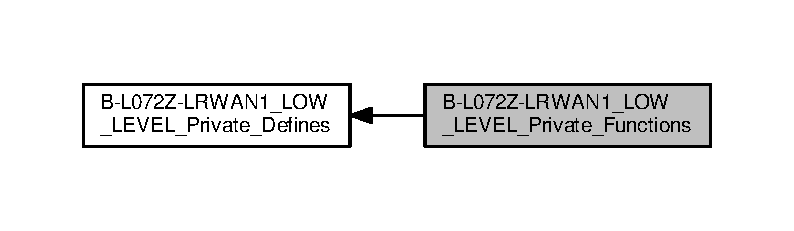
\includegraphics[width=350pt]{group__B-L072Z-LRWAN1__LOW__LEVEL__Private__Functions}
\end{center}
\end{figure}

\hypertarget{group__B-L072Z-LRWAN1__LOW__LEVEL__Exported__Types}{}\section{B-\/\+L072\+Z-\/\+L\+R\+W\+A\+N1\+\_\+\+L\+O\+W\+\_\+\+L\+E\+V\+E\+L\+\_\+\+Exported\+\_\+\+Types}
\label{group__B-L072Z-LRWAN1__LOW__LEVEL__Exported__Types}\index{B-\/\+L072\+Z-\/\+L\+R\+W\+A\+N1\+\_\+\+L\+O\+W\+\_\+\+L\+E\+V\+E\+L\+\_\+\+Exported\+\_\+\+Types@{B-\/\+L072\+Z-\/\+L\+R\+W\+A\+N1\+\_\+\+L\+O\+W\+\_\+\+L\+E\+V\+E\+L\+\_\+\+Exported\+\_\+\+Types}}
Collaboration diagram for B-\/\+L072\+Z-\/\+L\+R\+W\+A\+N1\+\_\+\+L\+O\+W\+\_\+\+L\+E\+V\+E\+L\+\_\+\+Exported\+\_\+\+Types\+:
\nopagebreak
\begin{figure}[H]
\begin{center}
\leavevmode
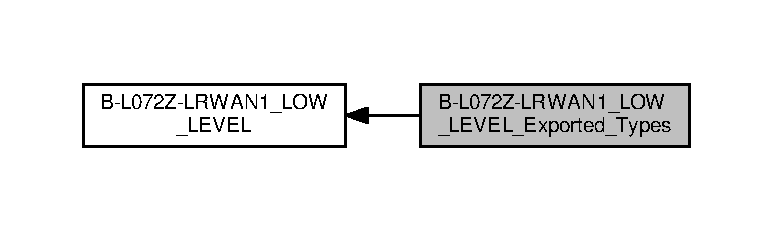
\includegraphics[width=350pt]{group__B-L072Z-LRWAN1__LOW__LEVEL__Exported__Types}
\end{center}
\end{figure}
\subsection*{Enumerations}
\begin{DoxyCompactItemize}
\item 
enum \hyperlink{group__B-L072Z-LRWAN1__LOW__LEVEL__Exported__Types_gaa059704b7ca945eb9c1e7f2c3d03fecd}{Led\+\_\+\+Type\+Def} \{ \newline
\hyperlink{group__B-L072Z-LRWAN1__LOW__LEVEL__Exported__Types_ggaa059704b7ca945eb9c1e7f2c3d03fecdadac6477842247cab1a8c02c65f431b44}{L\+E\+D1} = 0, 
\hyperlink{group__B-L072Z-LRWAN1__LOW__LEVEL__Exported__Types_ggaa059704b7ca945eb9c1e7f2c3d03fecda0ad916c7f80666dc88f6b5b22a72e742}{L\+E\+D\+\_\+\+G\+R\+E\+EN} = L\+E\+D1, 
\hyperlink{group__B-L072Z-LRWAN1__LOW__LEVEL__Exported__Types_ggaa059704b7ca945eb9c1e7f2c3d03fecda8379bbaa96d151e6adac488b2a147b7a}{L\+E\+D2} = 1, 
\hyperlink{group__B-L072Z-LRWAN1__LOW__LEVEL__Exported__Types_ggaa059704b7ca945eb9c1e7f2c3d03fecdaf706e3dc22e0cbc5d3c38bb45ee35922}{L\+E\+D\+\_\+\+R\+E\+D1} =L\+E\+D2, 
\newline
\hyperlink{group__B-L072Z-LRWAN1__LOW__LEVEL__Exported__Types_ggaa059704b7ca945eb9c1e7f2c3d03fecda5dec293e081e0fc78369c842fab8452b}{L\+E\+D3} = 2, 
\hyperlink{group__B-L072Z-LRWAN1__LOW__LEVEL__Exported__Types_ggaa059704b7ca945eb9c1e7f2c3d03fecdaa67c57c0ff22a2772cb6a5751a3327bf}{L\+E\+D\+\_\+\+B\+L\+UE} =L\+E\+D3, 
\hyperlink{group__B-L072Z-LRWAN1__LOW__LEVEL__Exported__Types_ggaa059704b7ca945eb9c1e7f2c3d03fecdad60e39b8d1701d30aa64f80343217342}{L\+E\+D4} = 3, 
\hyperlink{group__B-L072Z-LRWAN1__LOW__LEVEL__Exported__Types_ggaa059704b7ca945eb9c1e7f2c3d03fecdaa0ad02b3f991c643c1aa7db7cabd03e0}{L\+E\+D\+\_\+\+R\+E\+D2} =L\+E\+D4
 \}
\item 
enum \hyperlink{group__B-L072Z-LRWAN1__LOW__LEVEL__Exported__Types_ga643816dfbad5c734fc25a29ce8d35bb1}{Button\+\_\+\+Type\+Def} \{ \hyperlink{group__B-L072Z-LRWAN1__LOW__LEVEL__Exported__Types_gga643816dfbad5c734fc25a29ce8d35bb1a6454f3dfd31c55a877e1b6684451d076}{B\+U\+T\+T\+O\+N\+\_\+\+U\+S\+ER} = 0, 
\hyperlink{group__B-L072Z-LRWAN1__LOW__LEVEL__Exported__Types_gga643816dfbad5c734fc25a29ce8d35bb1a6ef88d3915166e6fc061a578a51eafd0}{B\+U\+T\+T\+O\+N\+\_\+\+K\+EY} = B\+U\+T\+T\+O\+N\+\_\+\+U\+S\+ER
 \}
\item 
enum \hyperlink{group__B-L072Z-LRWAN1__LOW__LEVEL__Exported__Types_ga48825b7c7d851c440ef8e808fd9d8f0a}{Button\+Mode\+\_\+\+Type\+Def} \{ \hyperlink{group__B-L072Z-LRWAN1__LOW__LEVEL__Exported__Types_gga48825b7c7d851c440ef8e808fd9d8f0aa9411f3542831027b24c493abfb998522}{B\+U\+T\+T\+O\+N\+\_\+\+M\+O\+D\+E\+\_\+\+G\+P\+IO} = 0, 
\hyperlink{group__B-L072Z-LRWAN1__LOW__LEVEL__Exported__Types_gga48825b7c7d851c440ef8e808fd9d8f0aa13c1ad97bc3db33d7f2b5a7c116bc8f5}{B\+U\+T\+T\+O\+N\+\_\+\+M\+O\+D\+E\+\_\+\+E\+X\+TI} = 1
 \}
\end{DoxyCompactItemize}


\subsection{Detailed Description}


\subsection{Enumeration Type Documentation}
\mbox{\Hypertarget{group__B-L072Z-LRWAN1__LOW__LEVEL__Exported__Types_ga643816dfbad5c734fc25a29ce8d35bb1}\label{group__B-L072Z-LRWAN1__LOW__LEVEL__Exported__Types_ga643816dfbad5c734fc25a29ce8d35bb1}} 
\index{B-\/\+L072\+Z-\/\+L\+R\+W\+A\+N1\+\_\+\+L\+O\+W\+\_\+\+L\+E\+V\+E\+L\+\_\+\+Exported\+\_\+\+Types@{B-\/\+L072\+Z-\/\+L\+R\+W\+A\+N1\+\_\+\+L\+O\+W\+\_\+\+L\+E\+V\+E\+L\+\_\+\+Exported\+\_\+\+Types}!Button\+\_\+\+Type\+Def@{Button\+\_\+\+Type\+Def}}
\index{Button\+\_\+\+Type\+Def@{Button\+\_\+\+Type\+Def}!B-\/\+L072\+Z-\/\+L\+R\+W\+A\+N1\+\_\+\+L\+O\+W\+\_\+\+L\+E\+V\+E\+L\+\_\+\+Exported\+\_\+\+Types@{B-\/\+L072\+Z-\/\+L\+R\+W\+A\+N1\+\_\+\+L\+O\+W\+\_\+\+L\+E\+V\+E\+L\+\_\+\+Exported\+\_\+\+Types}}
\subsubsection{\texorpdfstring{Button\+\_\+\+Type\+Def}{Button\_TypeDef}}
{\footnotesize\ttfamily enum \hyperlink{group__B-L072Z-LRWAN1__LOW__LEVEL__Exported__Types_ga643816dfbad5c734fc25a29ce8d35bb1}{Button\+\_\+\+Type\+Def}}

\begin{DoxyEnumFields}{Enumerator}
\raisebox{\heightof{T}}[0pt][0pt]{\index{B\+U\+T\+T\+O\+N\+\_\+\+U\+S\+ER@{B\+U\+T\+T\+O\+N\+\_\+\+U\+S\+ER}!B-\/\+L072\+Z-\/\+L\+R\+W\+A\+N1\+\_\+\+L\+O\+W\+\_\+\+L\+E\+V\+E\+L\+\_\+\+Exported\+\_\+\+Types@{B-\/\+L072\+Z-\/\+L\+R\+W\+A\+N1\+\_\+\+L\+O\+W\+\_\+\+L\+E\+V\+E\+L\+\_\+\+Exported\+\_\+\+Types}}\index{B-\/\+L072\+Z-\/\+L\+R\+W\+A\+N1\+\_\+\+L\+O\+W\+\_\+\+L\+E\+V\+E\+L\+\_\+\+Exported\+\_\+\+Types@{B-\/\+L072\+Z-\/\+L\+R\+W\+A\+N1\+\_\+\+L\+O\+W\+\_\+\+L\+E\+V\+E\+L\+\_\+\+Exported\+\_\+\+Types}!B\+U\+T\+T\+O\+N\+\_\+\+U\+S\+ER@{B\+U\+T\+T\+O\+N\+\_\+\+U\+S\+ER}}}\mbox{\Hypertarget{group__B-L072Z-LRWAN1__LOW__LEVEL__Exported__Types_gga643816dfbad5c734fc25a29ce8d35bb1a6454f3dfd31c55a877e1b6684451d076}\label{group__B-L072Z-LRWAN1__LOW__LEVEL__Exported__Types_gga643816dfbad5c734fc25a29ce8d35bb1a6454f3dfd31c55a877e1b6684451d076}} 
B\+U\+T\+T\+O\+N\+\_\+\+U\+S\+ER&\\
\hline

\raisebox{\heightof{T}}[0pt][0pt]{\index{B\+U\+T\+T\+O\+N\+\_\+\+K\+EY@{B\+U\+T\+T\+O\+N\+\_\+\+K\+EY}!B-\/\+L072\+Z-\/\+L\+R\+W\+A\+N1\+\_\+\+L\+O\+W\+\_\+\+L\+E\+V\+E\+L\+\_\+\+Exported\+\_\+\+Types@{B-\/\+L072\+Z-\/\+L\+R\+W\+A\+N1\+\_\+\+L\+O\+W\+\_\+\+L\+E\+V\+E\+L\+\_\+\+Exported\+\_\+\+Types}}\index{B-\/\+L072\+Z-\/\+L\+R\+W\+A\+N1\+\_\+\+L\+O\+W\+\_\+\+L\+E\+V\+E\+L\+\_\+\+Exported\+\_\+\+Types@{B-\/\+L072\+Z-\/\+L\+R\+W\+A\+N1\+\_\+\+L\+O\+W\+\_\+\+L\+E\+V\+E\+L\+\_\+\+Exported\+\_\+\+Types}!B\+U\+T\+T\+O\+N\+\_\+\+K\+EY@{B\+U\+T\+T\+O\+N\+\_\+\+K\+EY}}}\mbox{\Hypertarget{group__B-L072Z-LRWAN1__LOW__LEVEL__Exported__Types_gga643816dfbad5c734fc25a29ce8d35bb1a6ef88d3915166e6fc061a578a51eafd0}\label{group__B-L072Z-LRWAN1__LOW__LEVEL__Exported__Types_gga643816dfbad5c734fc25a29ce8d35bb1a6ef88d3915166e6fc061a578a51eafd0}} 
B\+U\+T\+T\+O\+N\+\_\+\+K\+EY&\\
\hline

\end{DoxyEnumFields}
\mbox{\Hypertarget{group__B-L072Z-LRWAN1__LOW__LEVEL__Exported__Types_ga48825b7c7d851c440ef8e808fd9d8f0a}\label{group__B-L072Z-LRWAN1__LOW__LEVEL__Exported__Types_ga48825b7c7d851c440ef8e808fd9d8f0a}} 
\index{B-\/\+L072\+Z-\/\+L\+R\+W\+A\+N1\+\_\+\+L\+O\+W\+\_\+\+L\+E\+V\+E\+L\+\_\+\+Exported\+\_\+\+Types@{B-\/\+L072\+Z-\/\+L\+R\+W\+A\+N1\+\_\+\+L\+O\+W\+\_\+\+L\+E\+V\+E\+L\+\_\+\+Exported\+\_\+\+Types}!Button\+Mode\+\_\+\+Type\+Def@{Button\+Mode\+\_\+\+Type\+Def}}
\index{Button\+Mode\+\_\+\+Type\+Def@{Button\+Mode\+\_\+\+Type\+Def}!B-\/\+L072\+Z-\/\+L\+R\+W\+A\+N1\+\_\+\+L\+O\+W\+\_\+\+L\+E\+V\+E\+L\+\_\+\+Exported\+\_\+\+Types@{B-\/\+L072\+Z-\/\+L\+R\+W\+A\+N1\+\_\+\+L\+O\+W\+\_\+\+L\+E\+V\+E\+L\+\_\+\+Exported\+\_\+\+Types}}
\subsubsection{\texorpdfstring{Button\+Mode\+\_\+\+Type\+Def}{ButtonMode\_TypeDef}}
{\footnotesize\ttfamily enum \hyperlink{group__B-L072Z-LRWAN1__LOW__LEVEL__Exported__Types_ga48825b7c7d851c440ef8e808fd9d8f0a}{Button\+Mode\+\_\+\+Type\+Def}}

\begin{DoxyEnumFields}{Enumerator}
\raisebox{\heightof{T}}[0pt][0pt]{\index{B\+U\+T\+T\+O\+N\+\_\+\+M\+O\+D\+E\+\_\+\+G\+P\+IO@{B\+U\+T\+T\+O\+N\+\_\+\+M\+O\+D\+E\+\_\+\+G\+P\+IO}!B-\/\+L072\+Z-\/\+L\+R\+W\+A\+N1\+\_\+\+L\+O\+W\+\_\+\+L\+E\+V\+E\+L\+\_\+\+Exported\+\_\+\+Types@{B-\/\+L072\+Z-\/\+L\+R\+W\+A\+N1\+\_\+\+L\+O\+W\+\_\+\+L\+E\+V\+E\+L\+\_\+\+Exported\+\_\+\+Types}}\index{B-\/\+L072\+Z-\/\+L\+R\+W\+A\+N1\+\_\+\+L\+O\+W\+\_\+\+L\+E\+V\+E\+L\+\_\+\+Exported\+\_\+\+Types@{B-\/\+L072\+Z-\/\+L\+R\+W\+A\+N1\+\_\+\+L\+O\+W\+\_\+\+L\+E\+V\+E\+L\+\_\+\+Exported\+\_\+\+Types}!B\+U\+T\+T\+O\+N\+\_\+\+M\+O\+D\+E\+\_\+\+G\+P\+IO@{B\+U\+T\+T\+O\+N\+\_\+\+M\+O\+D\+E\+\_\+\+G\+P\+IO}}}\mbox{\Hypertarget{group__B-L072Z-LRWAN1__LOW__LEVEL__Exported__Types_gga48825b7c7d851c440ef8e808fd9d8f0aa9411f3542831027b24c493abfb998522}\label{group__B-L072Z-LRWAN1__LOW__LEVEL__Exported__Types_gga48825b7c7d851c440ef8e808fd9d8f0aa9411f3542831027b24c493abfb998522}} 
B\+U\+T\+T\+O\+N\+\_\+\+M\+O\+D\+E\+\_\+\+G\+P\+IO&\\
\hline

\raisebox{\heightof{T}}[0pt][0pt]{\index{B\+U\+T\+T\+O\+N\+\_\+\+M\+O\+D\+E\+\_\+\+E\+X\+TI@{B\+U\+T\+T\+O\+N\+\_\+\+M\+O\+D\+E\+\_\+\+E\+X\+TI}!B-\/\+L072\+Z-\/\+L\+R\+W\+A\+N1\+\_\+\+L\+O\+W\+\_\+\+L\+E\+V\+E\+L\+\_\+\+Exported\+\_\+\+Types@{B-\/\+L072\+Z-\/\+L\+R\+W\+A\+N1\+\_\+\+L\+O\+W\+\_\+\+L\+E\+V\+E\+L\+\_\+\+Exported\+\_\+\+Types}}\index{B-\/\+L072\+Z-\/\+L\+R\+W\+A\+N1\+\_\+\+L\+O\+W\+\_\+\+L\+E\+V\+E\+L\+\_\+\+Exported\+\_\+\+Types@{B-\/\+L072\+Z-\/\+L\+R\+W\+A\+N1\+\_\+\+L\+O\+W\+\_\+\+L\+E\+V\+E\+L\+\_\+\+Exported\+\_\+\+Types}!B\+U\+T\+T\+O\+N\+\_\+\+M\+O\+D\+E\+\_\+\+E\+X\+TI@{B\+U\+T\+T\+O\+N\+\_\+\+M\+O\+D\+E\+\_\+\+E\+X\+TI}}}\mbox{\Hypertarget{group__B-L072Z-LRWAN1__LOW__LEVEL__Exported__Types_gga48825b7c7d851c440ef8e808fd9d8f0aa13c1ad97bc3db33d7f2b5a7c116bc8f5}\label{group__B-L072Z-LRWAN1__LOW__LEVEL__Exported__Types_gga48825b7c7d851c440ef8e808fd9d8f0aa13c1ad97bc3db33d7f2b5a7c116bc8f5}} 
B\+U\+T\+T\+O\+N\+\_\+\+M\+O\+D\+E\+\_\+\+E\+X\+TI&\\
\hline

\end{DoxyEnumFields}
\mbox{\Hypertarget{group__B-L072Z-LRWAN1__LOW__LEVEL__Exported__Types_gaa059704b7ca945eb9c1e7f2c3d03fecd}\label{group__B-L072Z-LRWAN1__LOW__LEVEL__Exported__Types_gaa059704b7ca945eb9c1e7f2c3d03fecd}} 
\index{B-\/\+L072\+Z-\/\+L\+R\+W\+A\+N1\+\_\+\+L\+O\+W\+\_\+\+L\+E\+V\+E\+L\+\_\+\+Exported\+\_\+\+Types@{B-\/\+L072\+Z-\/\+L\+R\+W\+A\+N1\+\_\+\+L\+O\+W\+\_\+\+L\+E\+V\+E\+L\+\_\+\+Exported\+\_\+\+Types}!Led\+\_\+\+Type\+Def@{Led\+\_\+\+Type\+Def}}
\index{Led\+\_\+\+Type\+Def@{Led\+\_\+\+Type\+Def}!B-\/\+L072\+Z-\/\+L\+R\+W\+A\+N1\+\_\+\+L\+O\+W\+\_\+\+L\+E\+V\+E\+L\+\_\+\+Exported\+\_\+\+Types@{B-\/\+L072\+Z-\/\+L\+R\+W\+A\+N1\+\_\+\+L\+O\+W\+\_\+\+L\+E\+V\+E\+L\+\_\+\+Exported\+\_\+\+Types}}
\subsubsection{\texorpdfstring{Led\+\_\+\+Type\+Def}{Led\_TypeDef}}
{\footnotesize\ttfamily enum \hyperlink{group__B-L072Z-LRWAN1__LOW__LEVEL__Exported__Types_gaa059704b7ca945eb9c1e7f2c3d03fecd}{Led\+\_\+\+Type\+Def}}

\begin{DoxyEnumFields}{Enumerator}
\raisebox{\heightof{T}}[0pt][0pt]{\index{L\+E\+D1@{L\+E\+D1}!B-\/\+L072\+Z-\/\+L\+R\+W\+A\+N1\+\_\+\+L\+O\+W\+\_\+\+L\+E\+V\+E\+L\+\_\+\+Exported\+\_\+\+Types@{B-\/\+L072\+Z-\/\+L\+R\+W\+A\+N1\+\_\+\+L\+O\+W\+\_\+\+L\+E\+V\+E\+L\+\_\+\+Exported\+\_\+\+Types}}\index{B-\/\+L072\+Z-\/\+L\+R\+W\+A\+N1\+\_\+\+L\+O\+W\+\_\+\+L\+E\+V\+E\+L\+\_\+\+Exported\+\_\+\+Types@{B-\/\+L072\+Z-\/\+L\+R\+W\+A\+N1\+\_\+\+L\+O\+W\+\_\+\+L\+E\+V\+E\+L\+\_\+\+Exported\+\_\+\+Types}!L\+E\+D1@{L\+E\+D1}}}\mbox{\Hypertarget{group__B-L072Z-LRWAN1__LOW__LEVEL__Exported__Types_ggaa059704b7ca945eb9c1e7f2c3d03fecdadac6477842247cab1a8c02c65f431b44}\label{group__B-L072Z-LRWAN1__LOW__LEVEL__Exported__Types_ggaa059704b7ca945eb9c1e7f2c3d03fecdadac6477842247cab1a8c02c65f431b44}} 
L\+E\+D1&\\
\hline

\raisebox{\heightof{T}}[0pt][0pt]{\index{L\+E\+D\+\_\+\+G\+R\+E\+EN@{L\+E\+D\+\_\+\+G\+R\+E\+EN}!B-\/\+L072\+Z-\/\+L\+R\+W\+A\+N1\+\_\+\+L\+O\+W\+\_\+\+L\+E\+V\+E\+L\+\_\+\+Exported\+\_\+\+Types@{B-\/\+L072\+Z-\/\+L\+R\+W\+A\+N1\+\_\+\+L\+O\+W\+\_\+\+L\+E\+V\+E\+L\+\_\+\+Exported\+\_\+\+Types}}\index{B-\/\+L072\+Z-\/\+L\+R\+W\+A\+N1\+\_\+\+L\+O\+W\+\_\+\+L\+E\+V\+E\+L\+\_\+\+Exported\+\_\+\+Types@{B-\/\+L072\+Z-\/\+L\+R\+W\+A\+N1\+\_\+\+L\+O\+W\+\_\+\+L\+E\+V\+E\+L\+\_\+\+Exported\+\_\+\+Types}!L\+E\+D\+\_\+\+G\+R\+E\+EN@{L\+E\+D\+\_\+\+G\+R\+E\+EN}}}\mbox{\Hypertarget{group__B-L072Z-LRWAN1__LOW__LEVEL__Exported__Types_ggaa059704b7ca945eb9c1e7f2c3d03fecda0ad916c7f80666dc88f6b5b22a72e742}\label{group__B-L072Z-LRWAN1__LOW__LEVEL__Exported__Types_ggaa059704b7ca945eb9c1e7f2c3d03fecda0ad916c7f80666dc88f6b5b22a72e742}} 
L\+E\+D\+\_\+\+G\+R\+E\+EN&\\
\hline

\raisebox{\heightof{T}}[0pt][0pt]{\index{L\+E\+D2@{L\+E\+D2}!B-\/\+L072\+Z-\/\+L\+R\+W\+A\+N1\+\_\+\+L\+O\+W\+\_\+\+L\+E\+V\+E\+L\+\_\+\+Exported\+\_\+\+Types@{B-\/\+L072\+Z-\/\+L\+R\+W\+A\+N1\+\_\+\+L\+O\+W\+\_\+\+L\+E\+V\+E\+L\+\_\+\+Exported\+\_\+\+Types}}\index{B-\/\+L072\+Z-\/\+L\+R\+W\+A\+N1\+\_\+\+L\+O\+W\+\_\+\+L\+E\+V\+E\+L\+\_\+\+Exported\+\_\+\+Types@{B-\/\+L072\+Z-\/\+L\+R\+W\+A\+N1\+\_\+\+L\+O\+W\+\_\+\+L\+E\+V\+E\+L\+\_\+\+Exported\+\_\+\+Types}!L\+E\+D2@{L\+E\+D2}}}\mbox{\Hypertarget{group__B-L072Z-LRWAN1__LOW__LEVEL__Exported__Types_ggaa059704b7ca945eb9c1e7f2c3d03fecda8379bbaa96d151e6adac488b2a147b7a}\label{group__B-L072Z-LRWAN1__LOW__LEVEL__Exported__Types_ggaa059704b7ca945eb9c1e7f2c3d03fecda8379bbaa96d151e6adac488b2a147b7a}} 
L\+E\+D2&\\
\hline

\raisebox{\heightof{T}}[0pt][0pt]{\index{L\+E\+D\+\_\+\+R\+E\+D1@{L\+E\+D\+\_\+\+R\+E\+D1}!B-\/\+L072\+Z-\/\+L\+R\+W\+A\+N1\+\_\+\+L\+O\+W\+\_\+\+L\+E\+V\+E\+L\+\_\+\+Exported\+\_\+\+Types@{B-\/\+L072\+Z-\/\+L\+R\+W\+A\+N1\+\_\+\+L\+O\+W\+\_\+\+L\+E\+V\+E\+L\+\_\+\+Exported\+\_\+\+Types}}\index{B-\/\+L072\+Z-\/\+L\+R\+W\+A\+N1\+\_\+\+L\+O\+W\+\_\+\+L\+E\+V\+E\+L\+\_\+\+Exported\+\_\+\+Types@{B-\/\+L072\+Z-\/\+L\+R\+W\+A\+N1\+\_\+\+L\+O\+W\+\_\+\+L\+E\+V\+E\+L\+\_\+\+Exported\+\_\+\+Types}!L\+E\+D\+\_\+\+R\+E\+D1@{L\+E\+D\+\_\+\+R\+E\+D1}}}\mbox{\Hypertarget{group__B-L072Z-LRWAN1__LOW__LEVEL__Exported__Types_ggaa059704b7ca945eb9c1e7f2c3d03fecdaf706e3dc22e0cbc5d3c38bb45ee35922}\label{group__B-L072Z-LRWAN1__LOW__LEVEL__Exported__Types_ggaa059704b7ca945eb9c1e7f2c3d03fecdaf706e3dc22e0cbc5d3c38bb45ee35922}} 
L\+E\+D\+\_\+\+R\+E\+D1&\\
\hline

\raisebox{\heightof{T}}[0pt][0pt]{\index{L\+E\+D3@{L\+E\+D3}!B-\/\+L072\+Z-\/\+L\+R\+W\+A\+N1\+\_\+\+L\+O\+W\+\_\+\+L\+E\+V\+E\+L\+\_\+\+Exported\+\_\+\+Types@{B-\/\+L072\+Z-\/\+L\+R\+W\+A\+N1\+\_\+\+L\+O\+W\+\_\+\+L\+E\+V\+E\+L\+\_\+\+Exported\+\_\+\+Types}}\index{B-\/\+L072\+Z-\/\+L\+R\+W\+A\+N1\+\_\+\+L\+O\+W\+\_\+\+L\+E\+V\+E\+L\+\_\+\+Exported\+\_\+\+Types@{B-\/\+L072\+Z-\/\+L\+R\+W\+A\+N1\+\_\+\+L\+O\+W\+\_\+\+L\+E\+V\+E\+L\+\_\+\+Exported\+\_\+\+Types}!L\+E\+D3@{L\+E\+D3}}}\mbox{\Hypertarget{group__B-L072Z-LRWAN1__LOW__LEVEL__Exported__Types_ggaa059704b7ca945eb9c1e7f2c3d03fecda5dec293e081e0fc78369c842fab8452b}\label{group__B-L072Z-LRWAN1__LOW__LEVEL__Exported__Types_ggaa059704b7ca945eb9c1e7f2c3d03fecda5dec293e081e0fc78369c842fab8452b}} 
L\+E\+D3&\\
\hline

\raisebox{\heightof{T}}[0pt][0pt]{\index{L\+E\+D\+\_\+\+B\+L\+UE@{L\+E\+D\+\_\+\+B\+L\+UE}!B-\/\+L072\+Z-\/\+L\+R\+W\+A\+N1\+\_\+\+L\+O\+W\+\_\+\+L\+E\+V\+E\+L\+\_\+\+Exported\+\_\+\+Types@{B-\/\+L072\+Z-\/\+L\+R\+W\+A\+N1\+\_\+\+L\+O\+W\+\_\+\+L\+E\+V\+E\+L\+\_\+\+Exported\+\_\+\+Types}}\index{B-\/\+L072\+Z-\/\+L\+R\+W\+A\+N1\+\_\+\+L\+O\+W\+\_\+\+L\+E\+V\+E\+L\+\_\+\+Exported\+\_\+\+Types@{B-\/\+L072\+Z-\/\+L\+R\+W\+A\+N1\+\_\+\+L\+O\+W\+\_\+\+L\+E\+V\+E\+L\+\_\+\+Exported\+\_\+\+Types}!L\+E\+D\+\_\+\+B\+L\+UE@{L\+E\+D\+\_\+\+B\+L\+UE}}}\mbox{\Hypertarget{group__B-L072Z-LRWAN1__LOW__LEVEL__Exported__Types_ggaa059704b7ca945eb9c1e7f2c3d03fecdaa67c57c0ff22a2772cb6a5751a3327bf}\label{group__B-L072Z-LRWAN1__LOW__LEVEL__Exported__Types_ggaa059704b7ca945eb9c1e7f2c3d03fecdaa67c57c0ff22a2772cb6a5751a3327bf}} 
L\+E\+D\+\_\+\+B\+L\+UE&\\
\hline

\raisebox{\heightof{T}}[0pt][0pt]{\index{L\+E\+D4@{L\+E\+D4}!B-\/\+L072\+Z-\/\+L\+R\+W\+A\+N1\+\_\+\+L\+O\+W\+\_\+\+L\+E\+V\+E\+L\+\_\+\+Exported\+\_\+\+Types@{B-\/\+L072\+Z-\/\+L\+R\+W\+A\+N1\+\_\+\+L\+O\+W\+\_\+\+L\+E\+V\+E\+L\+\_\+\+Exported\+\_\+\+Types}}\index{B-\/\+L072\+Z-\/\+L\+R\+W\+A\+N1\+\_\+\+L\+O\+W\+\_\+\+L\+E\+V\+E\+L\+\_\+\+Exported\+\_\+\+Types@{B-\/\+L072\+Z-\/\+L\+R\+W\+A\+N1\+\_\+\+L\+O\+W\+\_\+\+L\+E\+V\+E\+L\+\_\+\+Exported\+\_\+\+Types}!L\+E\+D4@{L\+E\+D4}}}\mbox{\Hypertarget{group__B-L072Z-LRWAN1__LOW__LEVEL__Exported__Types_ggaa059704b7ca945eb9c1e7f2c3d03fecdad60e39b8d1701d30aa64f80343217342}\label{group__B-L072Z-LRWAN1__LOW__LEVEL__Exported__Types_ggaa059704b7ca945eb9c1e7f2c3d03fecdad60e39b8d1701d30aa64f80343217342}} 
L\+E\+D4&\\
\hline

\raisebox{\heightof{T}}[0pt][0pt]{\index{L\+E\+D\+\_\+\+R\+E\+D2@{L\+E\+D\+\_\+\+R\+E\+D2}!B-\/\+L072\+Z-\/\+L\+R\+W\+A\+N1\+\_\+\+L\+O\+W\+\_\+\+L\+E\+V\+E\+L\+\_\+\+Exported\+\_\+\+Types@{B-\/\+L072\+Z-\/\+L\+R\+W\+A\+N1\+\_\+\+L\+O\+W\+\_\+\+L\+E\+V\+E\+L\+\_\+\+Exported\+\_\+\+Types}}\index{B-\/\+L072\+Z-\/\+L\+R\+W\+A\+N1\+\_\+\+L\+O\+W\+\_\+\+L\+E\+V\+E\+L\+\_\+\+Exported\+\_\+\+Types@{B-\/\+L072\+Z-\/\+L\+R\+W\+A\+N1\+\_\+\+L\+O\+W\+\_\+\+L\+E\+V\+E\+L\+\_\+\+Exported\+\_\+\+Types}!L\+E\+D\+\_\+\+R\+E\+D2@{L\+E\+D\+\_\+\+R\+E\+D2}}}\mbox{\Hypertarget{group__B-L072Z-LRWAN1__LOW__LEVEL__Exported__Types_ggaa059704b7ca945eb9c1e7f2c3d03fecdaa0ad02b3f991c643c1aa7db7cabd03e0}\label{group__B-L072Z-LRWAN1__LOW__LEVEL__Exported__Types_ggaa059704b7ca945eb9c1e7f2c3d03fecdaa0ad02b3f991c643c1aa7db7cabd03e0}} 
L\+E\+D\+\_\+\+R\+E\+D2&\\
\hline

\end{DoxyEnumFields}

\hypertarget{group__B-L072Z-LRWAN1__LOW__LEVEL__Exported__Constants}{}\section{B-\/\+L072\+Z-\/\+L\+R\+W\+A\+N1\+\_\+\+L\+O\+W\+\_\+\+L\+E\+V\+E\+L\+\_\+\+Exported\+\_\+\+Constants}
\label{group__B-L072Z-LRWAN1__LOW__LEVEL__Exported__Constants}\index{B-\/\+L072\+Z-\/\+L\+R\+W\+A\+N1\+\_\+\+L\+O\+W\+\_\+\+L\+E\+V\+E\+L\+\_\+\+Exported\+\_\+\+Constants@{B-\/\+L072\+Z-\/\+L\+R\+W\+A\+N1\+\_\+\+L\+O\+W\+\_\+\+L\+E\+V\+E\+L\+\_\+\+Exported\+\_\+\+Constants}}
Collaboration diagram for B-\/\+L072\+Z-\/\+L\+R\+W\+A\+N1\+\_\+\+L\+O\+W\+\_\+\+L\+E\+V\+E\+L\+\_\+\+Exported\+\_\+\+Constants\+:
\nopagebreak
\begin{figure}[H]
\begin{center}
\leavevmode
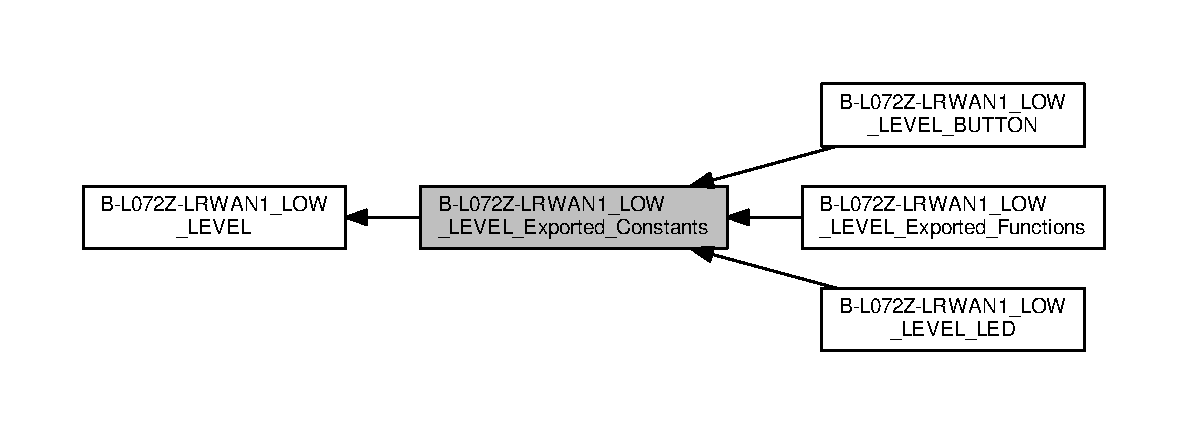
\includegraphics[width=350pt]{group__B-L072Z-LRWAN1__LOW__LEVEL__Exported__Constants}
\end{center}
\end{figure}
\subsection*{Modules}
\begin{DoxyCompactItemize}
\item 
\hyperlink{group__B-L072Z-LRWAN1__LOW__LEVEL__Exported__Functions}{B-\/\+L072\+Z-\/\+L\+R\+W\+A\+N1\+\_\+\+L\+O\+W\+\_\+\+L\+E\+V\+E\+L\+\_\+\+Exported\+\_\+\+Functions}
\item 
\hyperlink{group__B-L072Z-LRWAN1__LOW__LEVEL__LED}{B-\/\+L072\+Z-\/\+L\+R\+W\+A\+N1\+\_\+\+L\+O\+W\+\_\+\+L\+E\+V\+E\+L\+\_\+\+L\+ED}
\item 
\hyperlink{group__B-L072Z-LRWAN1__LOW__LEVEL__BUTTON}{B-\/\+L072\+Z-\/\+L\+R\+W\+A\+N1\+\_\+\+L\+O\+W\+\_\+\+L\+E\+V\+E\+L\+\_\+\+B\+U\+T\+T\+ON}
\end{DoxyCompactItemize}


\subsection{Detailed Description}

\hypertarget{group__B-L072Z-LRWAN1__LOW__LEVEL__Exported__Functions}{}\section{B-\/\+L072\+Z-\/\+L\+R\+W\+A\+N1\+\_\+\+L\+O\+W\+\_\+\+L\+E\+V\+E\+L\+\_\+\+Exported\+\_\+\+Functions}
\label{group__B-L072Z-LRWAN1__LOW__LEVEL__Exported__Functions}\index{B-\/\+L072\+Z-\/\+L\+R\+W\+A\+N1\+\_\+\+L\+O\+W\+\_\+\+L\+E\+V\+E\+L\+\_\+\+Exported\+\_\+\+Functions@{B-\/\+L072\+Z-\/\+L\+R\+W\+A\+N1\+\_\+\+L\+O\+W\+\_\+\+L\+E\+V\+E\+L\+\_\+\+Exported\+\_\+\+Functions}}
Collaboration diagram for B-\/\+L072\+Z-\/\+L\+R\+W\+A\+N1\+\_\+\+L\+O\+W\+\_\+\+L\+E\+V\+E\+L\+\_\+\+Exported\+\_\+\+Functions\+:
\nopagebreak
\begin{figure}[H]
\begin{center}
\leavevmode
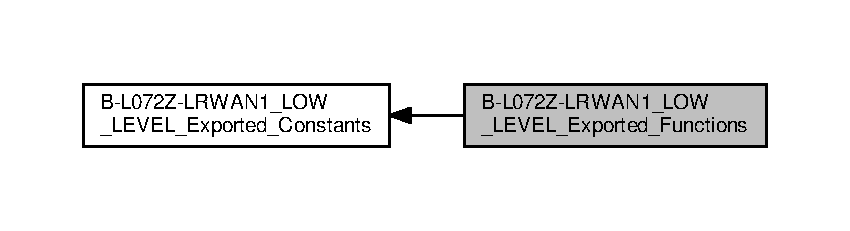
\includegraphics[width=350pt]{group__B-L072Z-LRWAN1__LOW__LEVEL__Exported__Functions}
\end{center}
\end{figure}
\subsection*{Functions}
\begin{DoxyCompactItemize}
\item 
uint32\+\_\+t \hyperlink{group__B-L072Z-LRWAN1__LOW__LEVEL__Exported__Functions_ga65d13608f7010a8068614154cb142cd6}{B\+S\+P\+\_\+\+Get\+Version} (void)
\begin{DoxyCompactList}\small\item\em This method returns the B-\/\+L072\+Z-\/\+L\+R\+W\+A\+N1 B\+SP Driver revision. \end{DoxyCompactList}\item 
void \hyperlink{group__B-L072Z-LRWAN1__LOW__LEVEL__Exported__Functions_gab58a4f16a476a53653c5c400e3bed158}{B\+S\+P\+\_\+\+L\+E\+D\+\_\+\+Init} (\hyperlink{group__B-L072Z-LRWAN1__LOW__LEVEL__Exported__Types_gaa059704b7ca945eb9c1e7f2c3d03fecd}{Led\+\_\+\+Type\+Def} Led)
\begin{DoxyCompactList}\small\item\em Configures L\+ED G\+P\+IO. \end{DoxyCompactList}\item 
void \hyperlink{group__B-L072Z-LRWAN1__LOW__LEVEL__Exported__Functions_gaee9c16b16384834c69efabf58f423d6f}{B\+S\+P\+\_\+\+L\+E\+D\+\_\+\+On} (\hyperlink{group__B-L072Z-LRWAN1__LOW__LEVEL__Exported__Types_gaa059704b7ca945eb9c1e7f2c3d03fecd}{Led\+\_\+\+Type\+Def} Led)
\begin{DoxyCompactList}\small\item\em Turns selected L\+ED On. \end{DoxyCompactList}\item 
void \hyperlink{group__B-L072Z-LRWAN1__LOW__LEVEL__Exported__Functions_gaef268680154ca15c45066d64d41f9467}{B\+S\+P\+\_\+\+L\+E\+D\+\_\+\+Off} (\hyperlink{group__B-L072Z-LRWAN1__LOW__LEVEL__Exported__Types_gaa059704b7ca945eb9c1e7f2c3d03fecd}{Led\+\_\+\+Type\+Def} Led)
\begin{DoxyCompactList}\small\item\em Turns selected L\+ED Off. \end{DoxyCompactList}\item 
void \hyperlink{group__B-L072Z-LRWAN1__LOW__LEVEL__Exported__Functions_ga1b9eabba7d498f41d6f16587ec0f9732}{B\+S\+P\+\_\+\+L\+E\+D\+\_\+\+Toggle} (\hyperlink{group__B-L072Z-LRWAN1__LOW__LEVEL__Exported__Types_gaa059704b7ca945eb9c1e7f2c3d03fecd}{Led\+\_\+\+Type\+Def} Led)
\begin{DoxyCompactList}\small\item\em Toggles the selected L\+ED. \end{DoxyCompactList}\item 
void \hyperlink{group__B-L072Z-LRWAN1__LOW__LEVEL__Exported__Functions_gacfde520fe598ece32657c56408354d2e}{B\+S\+P\+\_\+\+P\+B\+\_\+\+Init} (\hyperlink{group__B-L072Z-LRWAN1__LOW__LEVEL__Exported__Types_ga643816dfbad5c734fc25a29ce8d35bb1}{Button\+\_\+\+Type\+Def} Button, \hyperlink{group__B-L072Z-LRWAN1__LOW__LEVEL__Exported__Types_ga48825b7c7d851c440ef8e808fd9d8f0a}{Button\+Mode\+\_\+\+Type\+Def} Button\+\_\+\+Mode)
\begin{DoxyCompactList}\small\item\em Configures Button G\+P\+IO and E\+X\+TI Line. \end{DoxyCompactList}\item 
uint32\+\_\+t \hyperlink{group__B-L072Z-LRWAN1__LOW__LEVEL__Exported__Functions_ga8f0978b6cffda9c67266ddfdb3a0abf7}{B\+S\+P\+\_\+\+P\+B\+\_\+\+Get\+State} (\hyperlink{group__B-L072Z-LRWAN1__LOW__LEVEL__Exported__Types_ga643816dfbad5c734fc25a29ce8d35bb1}{Button\+\_\+\+Type\+Def} Button)
\begin{DoxyCompactList}\small\item\em Returns the selected Button state. \end{DoxyCompactList}\end{DoxyCompactItemize}


\subsection{Detailed Description}


\subsection{Function Documentation}
\mbox{\Hypertarget{group__B-L072Z-LRWAN1__LOW__LEVEL__Exported__Functions_ga65d13608f7010a8068614154cb142cd6}\label{group__B-L072Z-LRWAN1__LOW__LEVEL__Exported__Functions_ga65d13608f7010a8068614154cb142cd6}} 
\index{B-\/\+L072\+Z-\/\+L\+R\+W\+A\+N1\+\_\+\+L\+O\+W\+\_\+\+L\+E\+V\+E\+L\+\_\+\+Exported\+\_\+\+Functions@{B-\/\+L072\+Z-\/\+L\+R\+W\+A\+N1\+\_\+\+L\+O\+W\+\_\+\+L\+E\+V\+E\+L\+\_\+\+Exported\+\_\+\+Functions}!B\+S\+P\+\_\+\+Get\+Version@{B\+S\+P\+\_\+\+Get\+Version}}
\index{B\+S\+P\+\_\+\+Get\+Version@{B\+S\+P\+\_\+\+Get\+Version}!B-\/\+L072\+Z-\/\+L\+R\+W\+A\+N1\+\_\+\+L\+O\+W\+\_\+\+L\+E\+V\+E\+L\+\_\+\+Exported\+\_\+\+Functions@{B-\/\+L072\+Z-\/\+L\+R\+W\+A\+N1\+\_\+\+L\+O\+W\+\_\+\+L\+E\+V\+E\+L\+\_\+\+Exported\+\_\+\+Functions}}
\subsubsection{\texorpdfstring{B\+S\+P\+\_\+\+Get\+Version()}{BSP\_GetVersion()}}
{\footnotesize\ttfamily uint32\+\_\+t B\+S\+P\+\_\+\+Get\+Version (\begin{DoxyParamCaption}\item[{void}]{ }\end{DoxyParamCaption})}



This method returns the B-\/\+L072\+Z-\/\+L\+R\+W\+A\+N1 B\+SP Driver revision. 


\begin{DoxyParams}{Parameters}
{\em None} & \\
\hline
\end{DoxyParams}

\begin{DoxyRetVals}{Return values}
{\em version} & \+: 0x\+X\+Y\+ZR (8bits for each decimal, R for RC) \\
\hline
\end{DoxyRetVals}
\mbox{\Hypertarget{group__B-L072Z-LRWAN1__LOW__LEVEL__Exported__Functions_gab58a4f16a476a53653c5c400e3bed158}\label{group__B-L072Z-LRWAN1__LOW__LEVEL__Exported__Functions_gab58a4f16a476a53653c5c400e3bed158}} 
\index{B-\/\+L072\+Z-\/\+L\+R\+W\+A\+N1\+\_\+\+L\+O\+W\+\_\+\+L\+E\+V\+E\+L\+\_\+\+Exported\+\_\+\+Functions@{B-\/\+L072\+Z-\/\+L\+R\+W\+A\+N1\+\_\+\+L\+O\+W\+\_\+\+L\+E\+V\+E\+L\+\_\+\+Exported\+\_\+\+Functions}!B\+S\+P\+\_\+\+L\+E\+D\+\_\+\+Init@{B\+S\+P\+\_\+\+L\+E\+D\+\_\+\+Init}}
\index{B\+S\+P\+\_\+\+L\+E\+D\+\_\+\+Init@{B\+S\+P\+\_\+\+L\+E\+D\+\_\+\+Init}!B-\/\+L072\+Z-\/\+L\+R\+W\+A\+N1\+\_\+\+L\+O\+W\+\_\+\+L\+E\+V\+E\+L\+\_\+\+Exported\+\_\+\+Functions@{B-\/\+L072\+Z-\/\+L\+R\+W\+A\+N1\+\_\+\+L\+O\+W\+\_\+\+L\+E\+V\+E\+L\+\_\+\+Exported\+\_\+\+Functions}}
\subsubsection{\texorpdfstring{B\+S\+P\+\_\+\+L\+E\+D\+\_\+\+Init()}{BSP\_LED\_Init()}}
{\footnotesize\ttfamily void B\+S\+P\+\_\+\+L\+E\+D\+\_\+\+Init (\begin{DoxyParamCaption}\item[{\hyperlink{group__B-L072Z-LRWAN1__LOW__LEVEL__Exported__Types_gaa059704b7ca945eb9c1e7f2c3d03fecd}{Led\+\_\+\+Type\+Def}}]{Led }\end{DoxyParamCaption})}



Configures L\+ED G\+P\+IO. 


\begin{DoxyParams}{Parameters}
{\em Led} & Specifies the Led to be configured. This parameter can be one of following parameters\+: \begin{DoxyItemize}
\item L\+E\+D2 \end{DoxyItemize}
\\
\hline
\end{DoxyParams}

\begin{DoxyRetVals}{Return values}
{\em None} & \\
\hline
\end{DoxyRetVals}
\mbox{\Hypertarget{group__B-L072Z-LRWAN1__LOW__LEVEL__Exported__Functions_gaef268680154ca15c45066d64d41f9467}\label{group__B-L072Z-LRWAN1__LOW__LEVEL__Exported__Functions_gaef268680154ca15c45066d64d41f9467}} 
\index{B-\/\+L072\+Z-\/\+L\+R\+W\+A\+N1\+\_\+\+L\+O\+W\+\_\+\+L\+E\+V\+E\+L\+\_\+\+Exported\+\_\+\+Functions@{B-\/\+L072\+Z-\/\+L\+R\+W\+A\+N1\+\_\+\+L\+O\+W\+\_\+\+L\+E\+V\+E\+L\+\_\+\+Exported\+\_\+\+Functions}!B\+S\+P\+\_\+\+L\+E\+D\+\_\+\+Off@{B\+S\+P\+\_\+\+L\+E\+D\+\_\+\+Off}}
\index{B\+S\+P\+\_\+\+L\+E\+D\+\_\+\+Off@{B\+S\+P\+\_\+\+L\+E\+D\+\_\+\+Off}!B-\/\+L072\+Z-\/\+L\+R\+W\+A\+N1\+\_\+\+L\+O\+W\+\_\+\+L\+E\+V\+E\+L\+\_\+\+Exported\+\_\+\+Functions@{B-\/\+L072\+Z-\/\+L\+R\+W\+A\+N1\+\_\+\+L\+O\+W\+\_\+\+L\+E\+V\+E\+L\+\_\+\+Exported\+\_\+\+Functions}}
\subsubsection{\texorpdfstring{B\+S\+P\+\_\+\+L\+E\+D\+\_\+\+Off()}{BSP\_LED\_Off()}}
{\footnotesize\ttfamily void B\+S\+P\+\_\+\+L\+E\+D\+\_\+\+Off (\begin{DoxyParamCaption}\item[{\hyperlink{group__B-L072Z-LRWAN1__LOW__LEVEL__Exported__Types_gaa059704b7ca945eb9c1e7f2c3d03fecd}{Led\+\_\+\+Type\+Def}}]{Led }\end{DoxyParamCaption})}



Turns selected L\+ED Off. 


\begin{DoxyParams}{Parameters}
{\em Led} & Specifies the Led to be set off. This parameter can be one of following parameters\+: \begin{DoxyItemize}
\item L\+E\+D2 \end{DoxyItemize}
\\
\hline
\end{DoxyParams}

\begin{DoxyRetVals}{Return values}
{\em None} & \\
\hline
\end{DoxyRetVals}
\mbox{\Hypertarget{group__B-L072Z-LRWAN1__LOW__LEVEL__Exported__Functions_gaee9c16b16384834c69efabf58f423d6f}\label{group__B-L072Z-LRWAN1__LOW__LEVEL__Exported__Functions_gaee9c16b16384834c69efabf58f423d6f}} 
\index{B-\/\+L072\+Z-\/\+L\+R\+W\+A\+N1\+\_\+\+L\+O\+W\+\_\+\+L\+E\+V\+E\+L\+\_\+\+Exported\+\_\+\+Functions@{B-\/\+L072\+Z-\/\+L\+R\+W\+A\+N1\+\_\+\+L\+O\+W\+\_\+\+L\+E\+V\+E\+L\+\_\+\+Exported\+\_\+\+Functions}!B\+S\+P\+\_\+\+L\+E\+D\+\_\+\+On@{B\+S\+P\+\_\+\+L\+E\+D\+\_\+\+On}}
\index{B\+S\+P\+\_\+\+L\+E\+D\+\_\+\+On@{B\+S\+P\+\_\+\+L\+E\+D\+\_\+\+On}!B-\/\+L072\+Z-\/\+L\+R\+W\+A\+N1\+\_\+\+L\+O\+W\+\_\+\+L\+E\+V\+E\+L\+\_\+\+Exported\+\_\+\+Functions@{B-\/\+L072\+Z-\/\+L\+R\+W\+A\+N1\+\_\+\+L\+O\+W\+\_\+\+L\+E\+V\+E\+L\+\_\+\+Exported\+\_\+\+Functions}}
\subsubsection{\texorpdfstring{B\+S\+P\+\_\+\+L\+E\+D\+\_\+\+On()}{BSP\_LED\_On()}}
{\footnotesize\ttfamily void B\+S\+P\+\_\+\+L\+E\+D\+\_\+\+On (\begin{DoxyParamCaption}\item[{\hyperlink{group__B-L072Z-LRWAN1__LOW__LEVEL__Exported__Types_gaa059704b7ca945eb9c1e7f2c3d03fecd}{Led\+\_\+\+Type\+Def}}]{Led }\end{DoxyParamCaption})}



Turns selected L\+ED On. 


\begin{DoxyParams}{Parameters}
{\em Led} & Specifies the Led to be set on. This parameter can be one of following parameters\+: \begin{DoxyItemize}
\item L\+E\+D2 \end{DoxyItemize}
\\
\hline
\end{DoxyParams}

\begin{DoxyRetVals}{Return values}
{\em None} & \\
\hline
\end{DoxyRetVals}
\mbox{\Hypertarget{group__B-L072Z-LRWAN1__LOW__LEVEL__Exported__Functions_ga1b9eabba7d498f41d6f16587ec0f9732}\label{group__B-L072Z-LRWAN1__LOW__LEVEL__Exported__Functions_ga1b9eabba7d498f41d6f16587ec0f9732}} 
\index{B-\/\+L072\+Z-\/\+L\+R\+W\+A\+N1\+\_\+\+L\+O\+W\+\_\+\+L\+E\+V\+E\+L\+\_\+\+Exported\+\_\+\+Functions@{B-\/\+L072\+Z-\/\+L\+R\+W\+A\+N1\+\_\+\+L\+O\+W\+\_\+\+L\+E\+V\+E\+L\+\_\+\+Exported\+\_\+\+Functions}!B\+S\+P\+\_\+\+L\+E\+D\+\_\+\+Toggle@{B\+S\+P\+\_\+\+L\+E\+D\+\_\+\+Toggle}}
\index{B\+S\+P\+\_\+\+L\+E\+D\+\_\+\+Toggle@{B\+S\+P\+\_\+\+L\+E\+D\+\_\+\+Toggle}!B-\/\+L072\+Z-\/\+L\+R\+W\+A\+N1\+\_\+\+L\+O\+W\+\_\+\+L\+E\+V\+E\+L\+\_\+\+Exported\+\_\+\+Functions@{B-\/\+L072\+Z-\/\+L\+R\+W\+A\+N1\+\_\+\+L\+O\+W\+\_\+\+L\+E\+V\+E\+L\+\_\+\+Exported\+\_\+\+Functions}}
\subsubsection{\texorpdfstring{B\+S\+P\+\_\+\+L\+E\+D\+\_\+\+Toggle()}{BSP\_LED\_Toggle()}}
{\footnotesize\ttfamily void B\+S\+P\+\_\+\+L\+E\+D\+\_\+\+Toggle (\begin{DoxyParamCaption}\item[{\hyperlink{group__B-L072Z-LRWAN1__LOW__LEVEL__Exported__Types_gaa059704b7ca945eb9c1e7f2c3d03fecd}{Led\+\_\+\+Type\+Def}}]{Led }\end{DoxyParamCaption})}



Toggles the selected L\+ED. 


\begin{DoxyParams}{Parameters}
{\em Led} & Specifies the Led to be toggled. This parameter can be one of following parameters\+: \begin{DoxyItemize}
\item L\+E\+D2 \end{DoxyItemize}
\\
\hline
\end{DoxyParams}

\begin{DoxyRetVals}{Return values}
{\em None} & \\
\hline
\end{DoxyRetVals}
\mbox{\Hypertarget{group__B-L072Z-LRWAN1__LOW__LEVEL__Exported__Functions_ga8f0978b6cffda9c67266ddfdb3a0abf7}\label{group__B-L072Z-LRWAN1__LOW__LEVEL__Exported__Functions_ga8f0978b6cffda9c67266ddfdb3a0abf7}} 
\index{B-\/\+L072\+Z-\/\+L\+R\+W\+A\+N1\+\_\+\+L\+O\+W\+\_\+\+L\+E\+V\+E\+L\+\_\+\+Exported\+\_\+\+Functions@{B-\/\+L072\+Z-\/\+L\+R\+W\+A\+N1\+\_\+\+L\+O\+W\+\_\+\+L\+E\+V\+E\+L\+\_\+\+Exported\+\_\+\+Functions}!B\+S\+P\+\_\+\+P\+B\+\_\+\+Get\+State@{B\+S\+P\+\_\+\+P\+B\+\_\+\+Get\+State}}
\index{B\+S\+P\+\_\+\+P\+B\+\_\+\+Get\+State@{B\+S\+P\+\_\+\+P\+B\+\_\+\+Get\+State}!B-\/\+L072\+Z-\/\+L\+R\+W\+A\+N1\+\_\+\+L\+O\+W\+\_\+\+L\+E\+V\+E\+L\+\_\+\+Exported\+\_\+\+Functions@{B-\/\+L072\+Z-\/\+L\+R\+W\+A\+N1\+\_\+\+L\+O\+W\+\_\+\+L\+E\+V\+E\+L\+\_\+\+Exported\+\_\+\+Functions}}
\subsubsection{\texorpdfstring{B\+S\+P\+\_\+\+P\+B\+\_\+\+Get\+State()}{BSP\_PB\_GetState()}}
{\footnotesize\ttfamily uint32\+\_\+t B\+S\+P\+\_\+\+P\+B\+\_\+\+Get\+State (\begin{DoxyParamCaption}\item[{\hyperlink{group__B-L072Z-LRWAN1__LOW__LEVEL__Exported__Types_ga643816dfbad5c734fc25a29ce8d35bb1}{Button\+\_\+\+Type\+Def}}]{Button }\end{DoxyParamCaption})}



Returns the selected Button state. 


\begin{DoxyParams}{Parameters}
{\em Button} & Specifies the Button to be checked. This parameter should be\+: B\+U\+T\+T\+O\+N\+\_\+\+K\+EY \\
\hline
\end{DoxyParams}

\begin{DoxyRetVals}{Return values}
{\em The} & Button G\+P\+IO pin value. \\
\hline
\end{DoxyRetVals}
\mbox{\Hypertarget{group__B-L072Z-LRWAN1__LOW__LEVEL__Exported__Functions_gacfde520fe598ece32657c56408354d2e}\label{group__B-L072Z-LRWAN1__LOW__LEVEL__Exported__Functions_gacfde520fe598ece32657c56408354d2e}} 
\index{B-\/\+L072\+Z-\/\+L\+R\+W\+A\+N1\+\_\+\+L\+O\+W\+\_\+\+L\+E\+V\+E\+L\+\_\+\+Exported\+\_\+\+Functions@{B-\/\+L072\+Z-\/\+L\+R\+W\+A\+N1\+\_\+\+L\+O\+W\+\_\+\+L\+E\+V\+E\+L\+\_\+\+Exported\+\_\+\+Functions}!B\+S\+P\+\_\+\+P\+B\+\_\+\+Init@{B\+S\+P\+\_\+\+P\+B\+\_\+\+Init}}
\index{B\+S\+P\+\_\+\+P\+B\+\_\+\+Init@{B\+S\+P\+\_\+\+P\+B\+\_\+\+Init}!B-\/\+L072\+Z-\/\+L\+R\+W\+A\+N1\+\_\+\+L\+O\+W\+\_\+\+L\+E\+V\+E\+L\+\_\+\+Exported\+\_\+\+Functions@{B-\/\+L072\+Z-\/\+L\+R\+W\+A\+N1\+\_\+\+L\+O\+W\+\_\+\+L\+E\+V\+E\+L\+\_\+\+Exported\+\_\+\+Functions}}
\subsubsection{\texorpdfstring{B\+S\+P\+\_\+\+P\+B\+\_\+\+Init()}{BSP\_PB\_Init()}}
{\footnotesize\ttfamily void B\+S\+P\+\_\+\+P\+B\+\_\+\+Init (\begin{DoxyParamCaption}\item[{\hyperlink{group__B-L072Z-LRWAN1__LOW__LEVEL__Exported__Types_ga643816dfbad5c734fc25a29ce8d35bb1}{Button\+\_\+\+Type\+Def}}]{Button,  }\item[{\hyperlink{group__B-L072Z-LRWAN1__LOW__LEVEL__Exported__Types_ga48825b7c7d851c440ef8e808fd9d8f0a}{Button\+Mode\+\_\+\+Type\+Def}}]{Button\+Mode }\end{DoxyParamCaption})}



Configures Button G\+P\+IO and E\+X\+TI Line. 


\begin{DoxyParams}{Parameters}
{\em Button} & Specifies the Button to be configured. This parameter should be\+: B\+U\+T\+T\+O\+N\+\_\+\+K\+EY \\
\hline
{\em Button\+Mode} & Specifies Button mode. This parameter can be one of following parameters\+: \begin{DoxyItemize}
\item B\+U\+T\+T\+O\+N\+\_\+\+M\+O\+D\+E\+\_\+\+G\+P\+IO\+: Button will be used as simple IO \item B\+U\+T\+T\+O\+N\+\_\+\+M\+O\+D\+E\+\_\+\+E\+X\+TI\+: Button will be connected to E\+X\+TI line with interrupt generation capability \end{DoxyItemize}
\\
\hline
\end{DoxyParams}

\begin{DoxyRetVals}{Return values}
{\em None} & \\
\hline
\end{DoxyRetVals}

\hypertarget{group__BSP}{}\section{B\+SP}
\label{group__BSP}\index{B\+SP@{B\+SP}}
Collaboration diagram for B\+SP\+:
\nopagebreak
\begin{figure}[H]
\begin{center}
\leavevmode
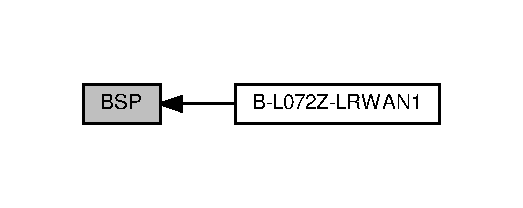
\includegraphics[width=251pt]{group__BSP}
\end{center}
\end{figure}
\subsection*{Modules}
\begin{DoxyCompactItemize}
\item 
\hyperlink{group__B-L072Z-LRWAN1}{B-\/\+L072\+Z-\/\+L\+R\+W\+A\+N1}
\end{DoxyCompactItemize}


\subsection{Detailed Description}

\hypertarget{group__B-L072Z-LRWAN1}{}\section{B-\/\+L072\+Z-\/\+L\+R\+W\+A\+N1}
\label{group__B-L072Z-LRWAN1}\index{B-\/\+L072\+Z-\/\+L\+R\+W\+A\+N1@{B-\/\+L072\+Z-\/\+L\+R\+W\+A\+N1}}
Collaboration diagram for B-\/\+L072\+Z-\/\+L\+R\+W\+A\+N1\+:
\nopagebreak
\begin{figure}[H]
\begin{center}
\leavevmode
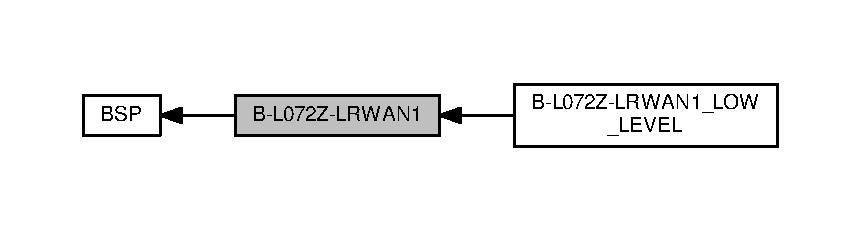
\includegraphics[width=350pt]{group__B-L072Z-LRWAN1}
\end{center}
\end{figure}
\subsection*{Modules}
\begin{DoxyCompactItemize}
\item 
\hyperlink{group__B-L072Z-LRWAN1__LOW__LEVEL}{B-\/\+L072\+Z-\/\+L\+R\+W\+A\+N1\+\_\+\+L\+O\+W\+\_\+\+L\+E\+V\+EL}
\begin{DoxyCompactList}\small\item\em This file provides set of firmware functions to manage Leds and push-\/button available on B-\/\+L072\+Z-\/\+L\+R\+W\+A\+N1 Discovery Kit from S\+T\+Microelectronics. \end{DoxyCompactList}\end{DoxyCompactItemize}


\subsection{Detailed Description}

\hypertarget{group__B-L072Z-LRWAN1__LOW__LEVEL}{}\section{B-\/\+L072\+Z-\/\+L\+R\+W\+A\+N1\+\_\+\+L\+O\+W\+\_\+\+L\+E\+V\+EL}
\label{group__B-L072Z-LRWAN1__LOW__LEVEL}\index{B-\/\+L072\+Z-\/\+L\+R\+W\+A\+N1\+\_\+\+L\+O\+W\+\_\+\+L\+E\+V\+EL@{B-\/\+L072\+Z-\/\+L\+R\+W\+A\+N1\+\_\+\+L\+O\+W\+\_\+\+L\+E\+V\+EL}}


This file provides set of firmware functions to manage Leds and push-\/button available on B-\/\+L072\+Z-\/\+L\+R\+W\+A\+N1 Discovery Kit from S\+T\+Microelectronics.  


Collaboration diagram for B-\/\+L072\+Z-\/\+L\+R\+W\+A\+N1\+\_\+\+L\+O\+W\+\_\+\+L\+E\+V\+EL\+:
\nopagebreak
\begin{figure}[H]
\begin{center}
\leavevmode
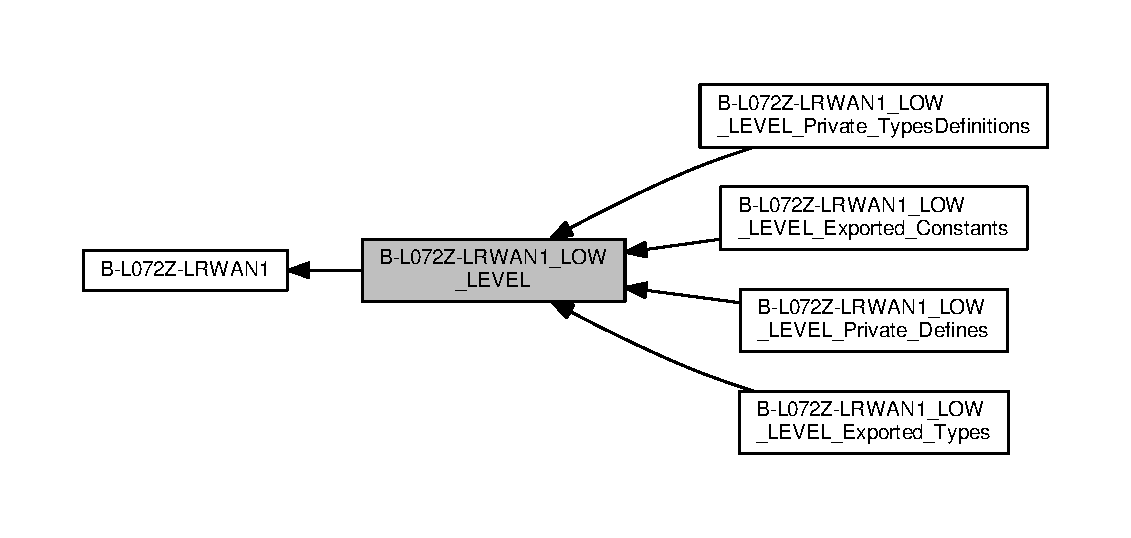
\includegraphics[width=350pt]{group__B-L072Z-LRWAN1__LOW__LEVEL}
\end{center}
\end{figure}
\subsection*{Modules}
\begin{DoxyCompactItemize}
\item 
\hyperlink{group__B-L072Z-LRWAN1__LOW__LEVEL__Private__TypesDefinitions}{B-\/\+L072\+Z-\/\+L\+R\+W\+A\+N1\+\_\+\+L\+O\+W\+\_\+\+L\+E\+V\+E\+L\+\_\+\+Private\+\_\+\+Types\+Definitions}
\item 
\hyperlink{group__B-L072Z-LRWAN1__LOW__LEVEL__Private__Defines}{B-\/\+L072\+Z-\/\+L\+R\+W\+A\+N1\+\_\+\+L\+O\+W\+\_\+\+L\+E\+V\+E\+L\+\_\+\+Private\+\_\+\+Defines}
\item 
\hyperlink{group__B-L072Z-LRWAN1__LOW__LEVEL__Exported__Types}{B-\/\+L072\+Z-\/\+L\+R\+W\+A\+N1\+\_\+\+L\+O\+W\+\_\+\+L\+E\+V\+E\+L\+\_\+\+Exported\+\_\+\+Types}
\item 
\hyperlink{group__B-L072Z-LRWAN1__LOW__LEVEL__Exported__Constants}{B-\/\+L072\+Z-\/\+L\+R\+W\+A\+N1\+\_\+\+L\+O\+W\+\_\+\+L\+E\+V\+E\+L\+\_\+\+Exported\+\_\+\+Constants}
\end{DoxyCompactItemize}


\subsection{Detailed Description}
This file provides set of firmware functions to manage Leds and push-\/button available on B-\/\+L072\+Z-\/\+L\+R\+W\+A\+N1 Discovery Kit from S\+T\+Microelectronics. 


\hypertarget{group__B-L072Z-LRWAN1__LOW__LEVEL__LED}{}\section{B-\/\+L072\+Z-\/\+L\+R\+W\+A\+N1\+\_\+\+L\+O\+W\+\_\+\+L\+E\+V\+E\+L\+\_\+\+L\+ED}
\label{group__B-L072Z-LRWAN1__LOW__LEVEL__LED}\index{B-\/\+L072\+Z-\/\+L\+R\+W\+A\+N1\+\_\+\+L\+O\+W\+\_\+\+L\+E\+V\+E\+L\+\_\+\+L\+ED@{B-\/\+L072\+Z-\/\+L\+R\+W\+A\+N1\+\_\+\+L\+O\+W\+\_\+\+L\+E\+V\+E\+L\+\_\+\+L\+ED}}
Collaboration diagram for B-\/\+L072\+Z-\/\+L\+R\+W\+A\+N1\+\_\+\+L\+O\+W\+\_\+\+L\+E\+V\+E\+L\+\_\+\+L\+ED\+:
\nopagebreak
\begin{figure}[H]
\begin{center}
\leavevmode
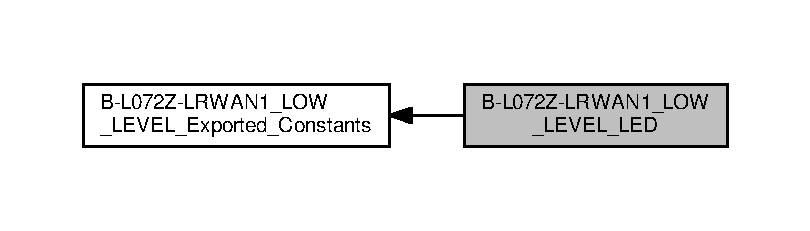
\includegraphics[width=350pt]{group__B-L072Z-LRWAN1__LOW__LEVEL__LED}
\end{center}
\end{figure}
\subsection*{Macros}
\begin{DoxyCompactItemize}
\item 
\#define \hyperlink{group__B-L072Z-LRWAN1__LOW__LEVEL__LED_gab4be2480bf7d44d52aab1190a65a733c}{L\+E\+Dn}~4
\item 
\#define \hyperlink{group__B-L072Z-LRWAN1__LOW__LEVEL__LED_ga318aa17e5d40e2132d2c7f6269ce7f51}{L\+E\+D1\+\_\+\+P\+IN}~G\+P\+I\+O\+\_\+\+P\+I\+N\+\_\+5
\item 
\#define \hyperlink{group__B-L072Z-LRWAN1__LOW__LEVEL__LED_ga5d97443b4011e40e47164445dc1adde0}{L\+E\+D1\+\_\+\+G\+P\+I\+O\+\_\+\+P\+O\+RT}~G\+P\+I\+OB
\item 
\#define \hyperlink{group__B-L072Z-LRWAN1__LOW__LEVEL__LED_gae90d969ab305110513ff3c2c0874f2e7}{L\+E\+D1\+\_\+\+G\+P\+I\+O\+\_\+\+C\+L\+K\+\_\+\+E\+N\+A\+B\+LE}()~\+\_\+\+\_\+\+H\+A\+L\+\_\+\+R\+C\+C\+\_\+\+G\+P\+I\+O\+B\+\_\+\+C\+L\+K\+\_\+\+E\+N\+A\+B\+LE()
\item 
\#define \hyperlink{group__B-L072Z-LRWAN1__LOW__LEVEL__LED_ga62e716eb8db20c4eccd17c29968d67c4}{L\+E\+D1\+\_\+\+G\+P\+I\+O\+\_\+\+C\+L\+K\+\_\+\+D\+I\+S\+A\+B\+LE}()~\+\_\+\+\_\+\+H\+A\+L\+\_\+\+R\+C\+C\+\_\+\+G\+P\+I\+O\+B\+\_\+\+C\+L\+K\+\_\+\+D\+I\+S\+A\+B\+LE()
\item 
\#define \hyperlink{group__B-L072Z-LRWAN1__LOW__LEVEL__LED_gaf6f84078113b55354d20585131b386f7}{L\+E\+D2\+\_\+\+P\+IN}~G\+P\+I\+O\+\_\+\+P\+I\+N\+\_\+5
\item 
\#define \hyperlink{group__B-L072Z-LRWAN1__LOW__LEVEL__LED_gaf88822ae4b79d37c7735ce1160b59f68}{L\+E\+D2\+\_\+\+G\+P\+I\+O\+\_\+\+P\+O\+RT}~G\+P\+I\+OA
\item 
\#define \hyperlink{group__B-L072Z-LRWAN1__LOW__LEVEL__LED_ga810e6c23b9a3e66da601b0058ec7a245}{L\+E\+D2\+\_\+\+G\+P\+I\+O\+\_\+\+C\+L\+K\+\_\+\+E\+N\+A\+B\+LE}()~\+\_\+\+\_\+\+H\+A\+L\+\_\+\+R\+C\+C\+\_\+\+G\+P\+I\+O\+A\+\_\+\+C\+L\+K\+\_\+\+E\+N\+A\+B\+LE()
\item 
\#define \hyperlink{group__B-L072Z-LRWAN1__LOW__LEVEL__LED_ga57f4d9343f3fe6d94d83ab2cb45c7d75}{L\+E\+D2\+\_\+\+G\+P\+I\+O\+\_\+\+C\+L\+K\+\_\+\+D\+I\+S\+A\+B\+LE}()~\+\_\+\+\_\+\+H\+A\+L\+\_\+\+R\+C\+C\+\_\+\+G\+P\+I\+O\+A\+\_\+\+C\+L\+K\+\_\+\+D\+I\+S\+A\+B\+LE()
\item 
\#define \hyperlink{group__B-L072Z-LRWAN1__LOW__LEVEL__LED_ga4cb3ff938bcabb01494ce529ae55a542}{L\+E\+D3\+\_\+\+P\+IN}~G\+P\+I\+O\+\_\+\+P\+I\+N\+\_\+6
\item 
\#define \hyperlink{group__B-L072Z-LRWAN1__LOW__LEVEL__LED_ga050f4b3a1f402476f9541dfe975d2143}{L\+E\+D3\+\_\+\+G\+P\+I\+O\+\_\+\+P\+O\+RT}~G\+P\+I\+OB
\item 
\#define \hyperlink{group__B-L072Z-LRWAN1__LOW__LEVEL__LED_gaac6c1162fc6bf1b60265e6fb7622e306}{L\+E\+D3\+\_\+\+G\+P\+I\+O\+\_\+\+C\+L\+K\+\_\+\+E\+N\+A\+B\+LE}()~\+\_\+\+\_\+\+H\+A\+L\+\_\+\+R\+C\+C\+\_\+\+G\+P\+I\+O\+B\+\_\+\+C\+L\+K\+\_\+\+E\+N\+A\+B\+LE()
\item 
\#define \hyperlink{group__B-L072Z-LRWAN1__LOW__LEVEL__LED_ga705278d726c1340f18576ca2d74f6e81}{L\+E\+D3\+\_\+\+G\+P\+I\+O\+\_\+\+C\+L\+K\+\_\+\+D\+I\+S\+A\+B\+LE}()~\+\_\+\+\_\+\+H\+A\+L\+\_\+\+R\+C\+C\+\_\+\+G\+P\+I\+O\+B\+\_\+\+C\+L\+K\+\_\+\+D\+I\+S\+A\+B\+LE()
\item 
\#define \hyperlink{group__B-L072Z-LRWAN1__LOW__LEVEL__LED_gaae684bb3d2f940637ccbc2adeb0e134d}{L\+E\+D4\+\_\+\+P\+IN}~G\+P\+I\+O\+\_\+\+P\+I\+N\+\_\+7
\item 
\#define \hyperlink{group__B-L072Z-LRWAN1__LOW__LEVEL__LED_ga6b6f3eb4d23b770de265803afbc2b61b}{L\+E\+D4\+\_\+\+G\+P\+I\+O\+\_\+\+P\+O\+RT}~G\+P\+I\+OB
\item 
\#define \hyperlink{group__B-L072Z-LRWAN1__LOW__LEVEL__LED_ga301aa5a187b24af8c121a462d2b08deb}{L\+E\+D4\+\_\+\+G\+P\+I\+O\+\_\+\+C\+L\+K\+\_\+\+E\+N\+A\+B\+LE}()~\+\_\+\+\_\+\+H\+A\+L\+\_\+\+R\+C\+C\+\_\+\+G\+P\+I\+O\+B\+\_\+\+C\+L\+K\+\_\+\+E\+N\+A\+B\+LE()
\item 
\#define \hyperlink{group__B-L072Z-LRWAN1__LOW__LEVEL__LED_ga9c737fb47feaa0f730edbe5251750353}{L\+E\+D4\+\_\+\+G\+P\+I\+O\+\_\+\+C\+L\+K\+\_\+\+D\+I\+S\+A\+B\+LE}()~\+\_\+\+\_\+\+H\+A\+L\+\_\+\+R\+C\+C\+\_\+\+G\+P\+I\+O\+B\+\_\+\+C\+L\+K\+\_\+\+D\+I\+S\+A\+B\+LE()
\item 
\#define \hyperlink{group__B-L072Z-LRWAN1__LOW__LEVEL__LED_ga32faaf3f04d44e7eddce1d781587fc57}{L\+E\+Dx\+\_\+\+G\+P\+I\+O\+\_\+\+C\+L\+K\+\_\+\+E\+N\+A\+B\+LE}(\+\_\+\+\_\+\+I\+N\+D\+E\+X\+\_\+\+\_\+)
\item 
\#define \hyperlink{group__B-L072Z-LRWAN1__LOW__LEVEL__LED_gaced1ef8f2a770d8c516ebc499b291df1}{L\+E\+Dx\+\_\+\+G\+P\+I\+O\+\_\+\+C\+L\+K\+\_\+\+D\+I\+S\+A\+B\+LE}(\+\_\+\+\_\+\+I\+N\+D\+E\+X\+\_\+\+\_\+)
\end{DoxyCompactItemize}


\subsection{Detailed Description}


\subsection{Macro Definition Documentation}
\mbox{\Hypertarget{group__B-L072Z-LRWAN1__LOW__LEVEL__LED_ga62e716eb8db20c4eccd17c29968d67c4}\label{group__B-L072Z-LRWAN1__LOW__LEVEL__LED_ga62e716eb8db20c4eccd17c29968d67c4}} 
\index{B-\/\+L072\+Z-\/\+L\+R\+W\+A\+N1\+\_\+\+L\+O\+W\+\_\+\+L\+E\+V\+E\+L\+\_\+\+L\+ED@{B-\/\+L072\+Z-\/\+L\+R\+W\+A\+N1\+\_\+\+L\+O\+W\+\_\+\+L\+E\+V\+E\+L\+\_\+\+L\+ED}!L\+E\+D1\+\_\+\+G\+P\+I\+O\+\_\+\+C\+L\+K\+\_\+\+D\+I\+S\+A\+B\+LE@{L\+E\+D1\+\_\+\+G\+P\+I\+O\+\_\+\+C\+L\+K\+\_\+\+D\+I\+S\+A\+B\+LE}}
\index{L\+E\+D1\+\_\+\+G\+P\+I\+O\+\_\+\+C\+L\+K\+\_\+\+D\+I\+S\+A\+B\+LE@{L\+E\+D1\+\_\+\+G\+P\+I\+O\+\_\+\+C\+L\+K\+\_\+\+D\+I\+S\+A\+B\+LE}!B-\/\+L072\+Z-\/\+L\+R\+W\+A\+N1\+\_\+\+L\+O\+W\+\_\+\+L\+E\+V\+E\+L\+\_\+\+L\+ED@{B-\/\+L072\+Z-\/\+L\+R\+W\+A\+N1\+\_\+\+L\+O\+W\+\_\+\+L\+E\+V\+E\+L\+\_\+\+L\+ED}}
\subsubsection{\texorpdfstring{L\+E\+D1\+\_\+\+G\+P\+I\+O\+\_\+\+C\+L\+K\+\_\+\+D\+I\+S\+A\+B\+LE}{LED1\_GPIO\_CLK\_DISABLE}}
{\footnotesize\ttfamily \#define L\+E\+D1\+\_\+\+G\+P\+I\+O\+\_\+\+C\+L\+K\+\_\+\+D\+I\+S\+A\+B\+LE(\begin{DoxyParamCaption}{ }\end{DoxyParamCaption})~\+\_\+\+\_\+\+H\+A\+L\+\_\+\+R\+C\+C\+\_\+\+G\+P\+I\+O\+B\+\_\+\+C\+L\+K\+\_\+\+D\+I\+S\+A\+B\+LE()}

\mbox{\Hypertarget{group__B-L072Z-LRWAN1__LOW__LEVEL__LED_gae90d969ab305110513ff3c2c0874f2e7}\label{group__B-L072Z-LRWAN1__LOW__LEVEL__LED_gae90d969ab305110513ff3c2c0874f2e7}} 
\index{B-\/\+L072\+Z-\/\+L\+R\+W\+A\+N1\+\_\+\+L\+O\+W\+\_\+\+L\+E\+V\+E\+L\+\_\+\+L\+ED@{B-\/\+L072\+Z-\/\+L\+R\+W\+A\+N1\+\_\+\+L\+O\+W\+\_\+\+L\+E\+V\+E\+L\+\_\+\+L\+ED}!L\+E\+D1\+\_\+\+G\+P\+I\+O\+\_\+\+C\+L\+K\+\_\+\+E\+N\+A\+B\+LE@{L\+E\+D1\+\_\+\+G\+P\+I\+O\+\_\+\+C\+L\+K\+\_\+\+E\+N\+A\+B\+LE}}
\index{L\+E\+D1\+\_\+\+G\+P\+I\+O\+\_\+\+C\+L\+K\+\_\+\+E\+N\+A\+B\+LE@{L\+E\+D1\+\_\+\+G\+P\+I\+O\+\_\+\+C\+L\+K\+\_\+\+E\+N\+A\+B\+LE}!B-\/\+L072\+Z-\/\+L\+R\+W\+A\+N1\+\_\+\+L\+O\+W\+\_\+\+L\+E\+V\+E\+L\+\_\+\+L\+ED@{B-\/\+L072\+Z-\/\+L\+R\+W\+A\+N1\+\_\+\+L\+O\+W\+\_\+\+L\+E\+V\+E\+L\+\_\+\+L\+ED}}
\subsubsection{\texorpdfstring{L\+E\+D1\+\_\+\+G\+P\+I\+O\+\_\+\+C\+L\+K\+\_\+\+E\+N\+A\+B\+LE}{LED1\_GPIO\_CLK\_ENABLE}}
{\footnotesize\ttfamily \#define L\+E\+D1\+\_\+\+G\+P\+I\+O\+\_\+\+C\+L\+K\+\_\+\+E\+N\+A\+B\+LE(\begin{DoxyParamCaption}{ }\end{DoxyParamCaption})~\+\_\+\+\_\+\+H\+A\+L\+\_\+\+R\+C\+C\+\_\+\+G\+P\+I\+O\+B\+\_\+\+C\+L\+K\+\_\+\+E\+N\+A\+B\+LE()}

\mbox{\Hypertarget{group__B-L072Z-LRWAN1__LOW__LEVEL__LED_ga5d97443b4011e40e47164445dc1adde0}\label{group__B-L072Z-LRWAN1__LOW__LEVEL__LED_ga5d97443b4011e40e47164445dc1adde0}} 
\index{B-\/\+L072\+Z-\/\+L\+R\+W\+A\+N1\+\_\+\+L\+O\+W\+\_\+\+L\+E\+V\+E\+L\+\_\+\+L\+ED@{B-\/\+L072\+Z-\/\+L\+R\+W\+A\+N1\+\_\+\+L\+O\+W\+\_\+\+L\+E\+V\+E\+L\+\_\+\+L\+ED}!L\+E\+D1\+\_\+\+G\+P\+I\+O\+\_\+\+P\+O\+RT@{L\+E\+D1\+\_\+\+G\+P\+I\+O\+\_\+\+P\+O\+RT}}
\index{L\+E\+D1\+\_\+\+G\+P\+I\+O\+\_\+\+P\+O\+RT@{L\+E\+D1\+\_\+\+G\+P\+I\+O\+\_\+\+P\+O\+RT}!B-\/\+L072\+Z-\/\+L\+R\+W\+A\+N1\+\_\+\+L\+O\+W\+\_\+\+L\+E\+V\+E\+L\+\_\+\+L\+ED@{B-\/\+L072\+Z-\/\+L\+R\+W\+A\+N1\+\_\+\+L\+O\+W\+\_\+\+L\+E\+V\+E\+L\+\_\+\+L\+ED}}
\subsubsection{\texorpdfstring{L\+E\+D1\+\_\+\+G\+P\+I\+O\+\_\+\+P\+O\+RT}{LED1\_GPIO\_PORT}}
{\footnotesize\ttfamily \#define L\+E\+D1\+\_\+\+G\+P\+I\+O\+\_\+\+P\+O\+RT~G\+P\+I\+OB}

\mbox{\Hypertarget{group__B-L072Z-LRWAN1__LOW__LEVEL__LED_ga318aa17e5d40e2132d2c7f6269ce7f51}\label{group__B-L072Z-LRWAN1__LOW__LEVEL__LED_ga318aa17e5d40e2132d2c7f6269ce7f51}} 
\index{B-\/\+L072\+Z-\/\+L\+R\+W\+A\+N1\+\_\+\+L\+O\+W\+\_\+\+L\+E\+V\+E\+L\+\_\+\+L\+ED@{B-\/\+L072\+Z-\/\+L\+R\+W\+A\+N1\+\_\+\+L\+O\+W\+\_\+\+L\+E\+V\+E\+L\+\_\+\+L\+ED}!L\+E\+D1\+\_\+\+P\+IN@{L\+E\+D1\+\_\+\+P\+IN}}
\index{L\+E\+D1\+\_\+\+P\+IN@{L\+E\+D1\+\_\+\+P\+IN}!B-\/\+L072\+Z-\/\+L\+R\+W\+A\+N1\+\_\+\+L\+O\+W\+\_\+\+L\+E\+V\+E\+L\+\_\+\+L\+ED@{B-\/\+L072\+Z-\/\+L\+R\+W\+A\+N1\+\_\+\+L\+O\+W\+\_\+\+L\+E\+V\+E\+L\+\_\+\+L\+ED}}
\subsubsection{\texorpdfstring{L\+E\+D1\+\_\+\+P\+IN}{LED1\_PIN}}
{\footnotesize\ttfamily \#define L\+E\+D1\+\_\+\+P\+IN~G\+P\+I\+O\+\_\+\+P\+I\+N\+\_\+5}

\mbox{\Hypertarget{group__B-L072Z-LRWAN1__LOW__LEVEL__LED_ga57f4d9343f3fe6d94d83ab2cb45c7d75}\label{group__B-L072Z-LRWAN1__LOW__LEVEL__LED_ga57f4d9343f3fe6d94d83ab2cb45c7d75}} 
\index{B-\/\+L072\+Z-\/\+L\+R\+W\+A\+N1\+\_\+\+L\+O\+W\+\_\+\+L\+E\+V\+E\+L\+\_\+\+L\+ED@{B-\/\+L072\+Z-\/\+L\+R\+W\+A\+N1\+\_\+\+L\+O\+W\+\_\+\+L\+E\+V\+E\+L\+\_\+\+L\+ED}!L\+E\+D2\+\_\+\+G\+P\+I\+O\+\_\+\+C\+L\+K\+\_\+\+D\+I\+S\+A\+B\+LE@{L\+E\+D2\+\_\+\+G\+P\+I\+O\+\_\+\+C\+L\+K\+\_\+\+D\+I\+S\+A\+B\+LE}}
\index{L\+E\+D2\+\_\+\+G\+P\+I\+O\+\_\+\+C\+L\+K\+\_\+\+D\+I\+S\+A\+B\+LE@{L\+E\+D2\+\_\+\+G\+P\+I\+O\+\_\+\+C\+L\+K\+\_\+\+D\+I\+S\+A\+B\+LE}!B-\/\+L072\+Z-\/\+L\+R\+W\+A\+N1\+\_\+\+L\+O\+W\+\_\+\+L\+E\+V\+E\+L\+\_\+\+L\+ED@{B-\/\+L072\+Z-\/\+L\+R\+W\+A\+N1\+\_\+\+L\+O\+W\+\_\+\+L\+E\+V\+E\+L\+\_\+\+L\+ED}}
\subsubsection{\texorpdfstring{L\+E\+D2\+\_\+\+G\+P\+I\+O\+\_\+\+C\+L\+K\+\_\+\+D\+I\+S\+A\+B\+LE}{LED2\_GPIO\_CLK\_DISABLE}}
{\footnotesize\ttfamily \#define L\+E\+D2\+\_\+\+G\+P\+I\+O\+\_\+\+C\+L\+K\+\_\+\+D\+I\+S\+A\+B\+LE(\begin{DoxyParamCaption}{ }\end{DoxyParamCaption})~\+\_\+\+\_\+\+H\+A\+L\+\_\+\+R\+C\+C\+\_\+\+G\+P\+I\+O\+A\+\_\+\+C\+L\+K\+\_\+\+D\+I\+S\+A\+B\+LE()}

\mbox{\Hypertarget{group__B-L072Z-LRWAN1__LOW__LEVEL__LED_ga810e6c23b9a3e66da601b0058ec7a245}\label{group__B-L072Z-LRWAN1__LOW__LEVEL__LED_ga810e6c23b9a3e66da601b0058ec7a245}} 
\index{B-\/\+L072\+Z-\/\+L\+R\+W\+A\+N1\+\_\+\+L\+O\+W\+\_\+\+L\+E\+V\+E\+L\+\_\+\+L\+ED@{B-\/\+L072\+Z-\/\+L\+R\+W\+A\+N1\+\_\+\+L\+O\+W\+\_\+\+L\+E\+V\+E\+L\+\_\+\+L\+ED}!L\+E\+D2\+\_\+\+G\+P\+I\+O\+\_\+\+C\+L\+K\+\_\+\+E\+N\+A\+B\+LE@{L\+E\+D2\+\_\+\+G\+P\+I\+O\+\_\+\+C\+L\+K\+\_\+\+E\+N\+A\+B\+LE}}
\index{L\+E\+D2\+\_\+\+G\+P\+I\+O\+\_\+\+C\+L\+K\+\_\+\+E\+N\+A\+B\+LE@{L\+E\+D2\+\_\+\+G\+P\+I\+O\+\_\+\+C\+L\+K\+\_\+\+E\+N\+A\+B\+LE}!B-\/\+L072\+Z-\/\+L\+R\+W\+A\+N1\+\_\+\+L\+O\+W\+\_\+\+L\+E\+V\+E\+L\+\_\+\+L\+ED@{B-\/\+L072\+Z-\/\+L\+R\+W\+A\+N1\+\_\+\+L\+O\+W\+\_\+\+L\+E\+V\+E\+L\+\_\+\+L\+ED}}
\subsubsection{\texorpdfstring{L\+E\+D2\+\_\+\+G\+P\+I\+O\+\_\+\+C\+L\+K\+\_\+\+E\+N\+A\+B\+LE}{LED2\_GPIO\_CLK\_ENABLE}}
{\footnotesize\ttfamily \#define L\+E\+D2\+\_\+\+G\+P\+I\+O\+\_\+\+C\+L\+K\+\_\+\+E\+N\+A\+B\+LE(\begin{DoxyParamCaption}{ }\end{DoxyParamCaption})~\+\_\+\+\_\+\+H\+A\+L\+\_\+\+R\+C\+C\+\_\+\+G\+P\+I\+O\+A\+\_\+\+C\+L\+K\+\_\+\+E\+N\+A\+B\+LE()}

\mbox{\Hypertarget{group__B-L072Z-LRWAN1__LOW__LEVEL__LED_gaf88822ae4b79d37c7735ce1160b59f68}\label{group__B-L072Z-LRWAN1__LOW__LEVEL__LED_gaf88822ae4b79d37c7735ce1160b59f68}} 
\index{B-\/\+L072\+Z-\/\+L\+R\+W\+A\+N1\+\_\+\+L\+O\+W\+\_\+\+L\+E\+V\+E\+L\+\_\+\+L\+ED@{B-\/\+L072\+Z-\/\+L\+R\+W\+A\+N1\+\_\+\+L\+O\+W\+\_\+\+L\+E\+V\+E\+L\+\_\+\+L\+ED}!L\+E\+D2\+\_\+\+G\+P\+I\+O\+\_\+\+P\+O\+RT@{L\+E\+D2\+\_\+\+G\+P\+I\+O\+\_\+\+P\+O\+RT}}
\index{L\+E\+D2\+\_\+\+G\+P\+I\+O\+\_\+\+P\+O\+RT@{L\+E\+D2\+\_\+\+G\+P\+I\+O\+\_\+\+P\+O\+RT}!B-\/\+L072\+Z-\/\+L\+R\+W\+A\+N1\+\_\+\+L\+O\+W\+\_\+\+L\+E\+V\+E\+L\+\_\+\+L\+ED@{B-\/\+L072\+Z-\/\+L\+R\+W\+A\+N1\+\_\+\+L\+O\+W\+\_\+\+L\+E\+V\+E\+L\+\_\+\+L\+ED}}
\subsubsection{\texorpdfstring{L\+E\+D2\+\_\+\+G\+P\+I\+O\+\_\+\+P\+O\+RT}{LED2\_GPIO\_PORT}}
{\footnotesize\ttfamily \#define L\+E\+D2\+\_\+\+G\+P\+I\+O\+\_\+\+P\+O\+RT~G\+P\+I\+OA}

\mbox{\Hypertarget{group__B-L072Z-LRWAN1__LOW__LEVEL__LED_gaf6f84078113b55354d20585131b386f7}\label{group__B-L072Z-LRWAN1__LOW__LEVEL__LED_gaf6f84078113b55354d20585131b386f7}} 
\index{B-\/\+L072\+Z-\/\+L\+R\+W\+A\+N1\+\_\+\+L\+O\+W\+\_\+\+L\+E\+V\+E\+L\+\_\+\+L\+ED@{B-\/\+L072\+Z-\/\+L\+R\+W\+A\+N1\+\_\+\+L\+O\+W\+\_\+\+L\+E\+V\+E\+L\+\_\+\+L\+ED}!L\+E\+D2\+\_\+\+P\+IN@{L\+E\+D2\+\_\+\+P\+IN}}
\index{L\+E\+D2\+\_\+\+P\+IN@{L\+E\+D2\+\_\+\+P\+IN}!B-\/\+L072\+Z-\/\+L\+R\+W\+A\+N1\+\_\+\+L\+O\+W\+\_\+\+L\+E\+V\+E\+L\+\_\+\+L\+ED@{B-\/\+L072\+Z-\/\+L\+R\+W\+A\+N1\+\_\+\+L\+O\+W\+\_\+\+L\+E\+V\+E\+L\+\_\+\+L\+ED}}
\subsubsection{\texorpdfstring{L\+E\+D2\+\_\+\+P\+IN}{LED2\_PIN}}
{\footnotesize\ttfamily \#define L\+E\+D2\+\_\+\+P\+IN~G\+P\+I\+O\+\_\+\+P\+I\+N\+\_\+5}

\mbox{\Hypertarget{group__B-L072Z-LRWAN1__LOW__LEVEL__LED_ga705278d726c1340f18576ca2d74f6e81}\label{group__B-L072Z-LRWAN1__LOW__LEVEL__LED_ga705278d726c1340f18576ca2d74f6e81}} 
\index{B-\/\+L072\+Z-\/\+L\+R\+W\+A\+N1\+\_\+\+L\+O\+W\+\_\+\+L\+E\+V\+E\+L\+\_\+\+L\+ED@{B-\/\+L072\+Z-\/\+L\+R\+W\+A\+N1\+\_\+\+L\+O\+W\+\_\+\+L\+E\+V\+E\+L\+\_\+\+L\+ED}!L\+E\+D3\+\_\+\+G\+P\+I\+O\+\_\+\+C\+L\+K\+\_\+\+D\+I\+S\+A\+B\+LE@{L\+E\+D3\+\_\+\+G\+P\+I\+O\+\_\+\+C\+L\+K\+\_\+\+D\+I\+S\+A\+B\+LE}}
\index{L\+E\+D3\+\_\+\+G\+P\+I\+O\+\_\+\+C\+L\+K\+\_\+\+D\+I\+S\+A\+B\+LE@{L\+E\+D3\+\_\+\+G\+P\+I\+O\+\_\+\+C\+L\+K\+\_\+\+D\+I\+S\+A\+B\+LE}!B-\/\+L072\+Z-\/\+L\+R\+W\+A\+N1\+\_\+\+L\+O\+W\+\_\+\+L\+E\+V\+E\+L\+\_\+\+L\+ED@{B-\/\+L072\+Z-\/\+L\+R\+W\+A\+N1\+\_\+\+L\+O\+W\+\_\+\+L\+E\+V\+E\+L\+\_\+\+L\+ED}}
\subsubsection{\texorpdfstring{L\+E\+D3\+\_\+\+G\+P\+I\+O\+\_\+\+C\+L\+K\+\_\+\+D\+I\+S\+A\+B\+LE}{LED3\_GPIO\_CLK\_DISABLE}}
{\footnotesize\ttfamily \#define L\+E\+D3\+\_\+\+G\+P\+I\+O\+\_\+\+C\+L\+K\+\_\+\+D\+I\+S\+A\+B\+LE(\begin{DoxyParamCaption}{ }\end{DoxyParamCaption})~\+\_\+\+\_\+\+H\+A\+L\+\_\+\+R\+C\+C\+\_\+\+G\+P\+I\+O\+B\+\_\+\+C\+L\+K\+\_\+\+D\+I\+S\+A\+B\+LE()}

\mbox{\Hypertarget{group__B-L072Z-LRWAN1__LOW__LEVEL__LED_gaac6c1162fc6bf1b60265e6fb7622e306}\label{group__B-L072Z-LRWAN1__LOW__LEVEL__LED_gaac6c1162fc6bf1b60265e6fb7622e306}} 
\index{B-\/\+L072\+Z-\/\+L\+R\+W\+A\+N1\+\_\+\+L\+O\+W\+\_\+\+L\+E\+V\+E\+L\+\_\+\+L\+ED@{B-\/\+L072\+Z-\/\+L\+R\+W\+A\+N1\+\_\+\+L\+O\+W\+\_\+\+L\+E\+V\+E\+L\+\_\+\+L\+ED}!L\+E\+D3\+\_\+\+G\+P\+I\+O\+\_\+\+C\+L\+K\+\_\+\+E\+N\+A\+B\+LE@{L\+E\+D3\+\_\+\+G\+P\+I\+O\+\_\+\+C\+L\+K\+\_\+\+E\+N\+A\+B\+LE}}
\index{L\+E\+D3\+\_\+\+G\+P\+I\+O\+\_\+\+C\+L\+K\+\_\+\+E\+N\+A\+B\+LE@{L\+E\+D3\+\_\+\+G\+P\+I\+O\+\_\+\+C\+L\+K\+\_\+\+E\+N\+A\+B\+LE}!B-\/\+L072\+Z-\/\+L\+R\+W\+A\+N1\+\_\+\+L\+O\+W\+\_\+\+L\+E\+V\+E\+L\+\_\+\+L\+ED@{B-\/\+L072\+Z-\/\+L\+R\+W\+A\+N1\+\_\+\+L\+O\+W\+\_\+\+L\+E\+V\+E\+L\+\_\+\+L\+ED}}
\subsubsection{\texorpdfstring{L\+E\+D3\+\_\+\+G\+P\+I\+O\+\_\+\+C\+L\+K\+\_\+\+E\+N\+A\+B\+LE}{LED3\_GPIO\_CLK\_ENABLE}}
{\footnotesize\ttfamily \#define L\+E\+D3\+\_\+\+G\+P\+I\+O\+\_\+\+C\+L\+K\+\_\+\+E\+N\+A\+B\+LE(\begin{DoxyParamCaption}{ }\end{DoxyParamCaption})~\+\_\+\+\_\+\+H\+A\+L\+\_\+\+R\+C\+C\+\_\+\+G\+P\+I\+O\+B\+\_\+\+C\+L\+K\+\_\+\+E\+N\+A\+B\+LE()}

\mbox{\Hypertarget{group__B-L072Z-LRWAN1__LOW__LEVEL__LED_ga050f4b3a1f402476f9541dfe975d2143}\label{group__B-L072Z-LRWAN1__LOW__LEVEL__LED_ga050f4b3a1f402476f9541dfe975d2143}} 
\index{B-\/\+L072\+Z-\/\+L\+R\+W\+A\+N1\+\_\+\+L\+O\+W\+\_\+\+L\+E\+V\+E\+L\+\_\+\+L\+ED@{B-\/\+L072\+Z-\/\+L\+R\+W\+A\+N1\+\_\+\+L\+O\+W\+\_\+\+L\+E\+V\+E\+L\+\_\+\+L\+ED}!L\+E\+D3\+\_\+\+G\+P\+I\+O\+\_\+\+P\+O\+RT@{L\+E\+D3\+\_\+\+G\+P\+I\+O\+\_\+\+P\+O\+RT}}
\index{L\+E\+D3\+\_\+\+G\+P\+I\+O\+\_\+\+P\+O\+RT@{L\+E\+D3\+\_\+\+G\+P\+I\+O\+\_\+\+P\+O\+RT}!B-\/\+L072\+Z-\/\+L\+R\+W\+A\+N1\+\_\+\+L\+O\+W\+\_\+\+L\+E\+V\+E\+L\+\_\+\+L\+ED@{B-\/\+L072\+Z-\/\+L\+R\+W\+A\+N1\+\_\+\+L\+O\+W\+\_\+\+L\+E\+V\+E\+L\+\_\+\+L\+ED}}
\subsubsection{\texorpdfstring{L\+E\+D3\+\_\+\+G\+P\+I\+O\+\_\+\+P\+O\+RT}{LED3\_GPIO\_PORT}}
{\footnotesize\ttfamily \#define L\+E\+D3\+\_\+\+G\+P\+I\+O\+\_\+\+P\+O\+RT~G\+P\+I\+OB}

\mbox{\Hypertarget{group__B-L072Z-LRWAN1__LOW__LEVEL__LED_ga4cb3ff938bcabb01494ce529ae55a542}\label{group__B-L072Z-LRWAN1__LOW__LEVEL__LED_ga4cb3ff938bcabb01494ce529ae55a542}} 
\index{B-\/\+L072\+Z-\/\+L\+R\+W\+A\+N1\+\_\+\+L\+O\+W\+\_\+\+L\+E\+V\+E\+L\+\_\+\+L\+ED@{B-\/\+L072\+Z-\/\+L\+R\+W\+A\+N1\+\_\+\+L\+O\+W\+\_\+\+L\+E\+V\+E\+L\+\_\+\+L\+ED}!L\+E\+D3\+\_\+\+P\+IN@{L\+E\+D3\+\_\+\+P\+IN}}
\index{L\+E\+D3\+\_\+\+P\+IN@{L\+E\+D3\+\_\+\+P\+IN}!B-\/\+L072\+Z-\/\+L\+R\+W\+A\+N1\+\_\+\+L\+O\+W\+\_\+\+L\+E\+V\+E\+L\+\_\+\+L\+ED@{B-\/\+L072\+Z-\/\+L\+R\+W\+A\+N1\+\_\+\+L\+O\+W\+\_\+\+L\+E\+V\+E\+L\+\_\+\+L\+ED}}
\subsubsection{\texorpdfstring{L\+E\+D3\+\_\+\+P\+IN}{LED3\_PIN}}
{\footnotesize\ttfamily \#define L\+E\+D3\+\_\+\+P\+IN~G\+P\+I\+O\+\_\+\+P\+I\+N\+\_\+6}

\mbox{\Hypertarget{group__B-L072Z-LRWAN1__LOW__LEVEL__LED_ga9c737fb47feaa0f730edbe5251750353}\label{group__B-L072Z-LRWAN1__LOW__LEVEL__LED_ga9c737fb47feaa0f730edbe5251750353}} 
\index{B-\/\+L072\+Z-\/\+L\+R\+W\+A\+N1\+\_\+\+L\+O\+W\+\_\+\+L\+E\+V\+E\+L\+\_\+\+L\+ED@{B-\/\+L072\+Z-\/\+L\+R\+W\+A\+N1\+\_\+\+L\+O\+W\+\_\+\+L\+E\+V\+E\+L\+\_\+\+L\+ED}!L\+E\+D4\+\_\+\+G\+P\+I\+O\+\_\+\+C\+L\+K\+\_\+\+D\+I\+S\+A\+B\+LE@{L\+E\+D4\+\_\+\+G\+P\+I\+O\+\_\+\+C\+L\+K\+\_\+\+D\+I\+S\+A\+B\+LE}}
\index{L\+E\+D4\+\_\+\+G\+P\+I\+O\+\_\+\+C\+L\+K\+\_\+\+D\+I\+S\+A\+B\+LE@{L\+E\+D4\+\_\+\+G\+P\+I\+O\+\_\+\+C\+L\+K\+\_\+\+D\+I\+S\+A\+B\+LE}!B-\/\+L072\+Z-\/\+L\+R\+W\+A\+N1\+\_\+\+L\+O\+W\+\_\+\+L\+E\+V\+E\+L\+\_\+\+L\+ED@{B-\/\+L072\+Z-\/\+L\+R\+W\+A\+N1\+\_\+\+L\+O\+W\+\_\+\+L\+E\+V\+E\+L\+\_\+\+L\+ED}}
\subsubsection{\texorpdfstring{L\+E\+D4\+\_\+\+G\+P\+I\+O\+\_\+\+C\+L\+K\+\_\+\+D\+I\+S\+A\+B\+LE}{LED4\_GPIO\_CLK\_DISABLE}}
{\footnotesize\ttfamily \#define L\+E\+D4\+\_\+\+G\+P\+I\+O\+\_\+\+C\+L\+K\+\_\+\+D\+I\+S\+A\+B\+LE(\begin{DoxyParamCaption}{ }\end{DoxyParamCaption})~\+\_\+\+\_\+\+H\+A\+L\+\_\+\+R\+C\+C\+\_\+\+G\+P\+I\+O\+B\+\_\+\+C\+L\+K\+\_\+\+D\+I\+S\+A\+B\+LE()}

\mbox{\Hypertarget{group__B-L072Z-LRWAN1__LOW__LEVEL__LED_ga301aa5a187b24af8c121a462d2b08deb}\label{group__B-L072Z-LRWAN1__LOW__LEVEL__LED_ga301aa5a187b24af8c121a462d2b08deb}} 
\index{B-\/\+L072\+Z-\/\+L\+R\+W\+A\+N1\+\_\+\+L\+O\+W\+\_\+\+L\+E\+V\+E\+L\+\_\+\+L\+ED@{B-\/\+L072\+Z-\/\+L\+R\+W\+A\+N1\+\_\+\+L\+O\+W\+\_\+\+L\+E\+V\+E\+L\+\_\+\+L\+ED}!L\+E\+D4\+\_\+\+G\+P\+I\+O\+\_\+\+C\+L\+K\+\_\+\+E\+N\+A\+B\+LE@{L\+E\+D4\+\_\+\+G\+P\+I\+O\+\_\+\+C\+L\+K\+\_\+\+E\+N\+A\+B\+LE}}
\index{L\+E\+D4\+\_\+\+G\+P\+I\+O\+\_\+\+C\+L\+K\+\_\+\+E\+N\+A\+B\+LE@{L\+E\+D4\+\_\+\+G\+P\+I\+O\+\_\+\+C\+L\+K\+\_\+\+E\+N\+A\+B\+LE}!B-\/\+L072\+Z-\/\+L\+R\+W\+A\+N1\+\_\+\+L\+O\+W\+\_\+\+L\+E\+V\+E\+L\+\_\+\+L\+ED@{B-\/\+L072\+Z-\/\+L\+R\+W\+A\+N1\+\_\+\+L\+O\+W\+\_\+\+L\+E\+V\+E\+L\+\_\+\+L\+ED}}
\subsubsection{\texorpdfstring{L\+E\+D4\+\_\+\+G\+P\+I\+O\+\_\+\+C\+L\+K\+\_\+\+E\+N\+A\+B\+LE}{LED4\_GPIO\_CLK\_ENABLE}}
{\footnotesize\ttfamily \#define L\+E\+D4\+\_\+\+G\+P\+I\+O\+\_\+\+C\+L\+K\+\_\+\+E\+N\+A\+B\+LE(\begin{DoxyParamCaption}{ }\end{DoxyParamCaption})~\+\_\+\+\_\+\+H\+A\+L\+\_\+\+R\+C\+C\+\_\+\+G\+P\+I\+O\+B\+\_\+\+C\+L\+K\+\_\+\+E\+N\+A\+B\+LE()}

\mbox{\Hypertarget{group__B-L072Z-LRWAN1__LOW__LEVEL__LED_ga6b6f3eb4d23b770de265803afbc2b61b}\label{group__B-L072Z-LRWAN1__LOW__LEVEL__LED_ga6b6f3eb4d23b770de265803afbc2b61b}} 
\index{B-\/\+L072\+Z-\/\+L\+R\+W\+A\+N1\+\_\+\+L\+O\+W\+\_\+\+L\+E\+V\+E\+L\+\_\+\+L\+ED@{B-\/\+L072\+Z-\/\+L\+R\+W\+A\+N1\+\_\+\+L\+O\+W\+\_\+\+L\+E\+V\+E\+L\+\_\+\+L\+ED}!L\+E\+D4\+\_\+\+G\+P\+I\+O\+\_\+\+P\+O\+RT@{L\+E\+D4\+\_\+\+G\+P\+I\+O\+\_\+\+P\+O\+RT}}
\index{L\+E\+D4\+\_\+\+G\+P\+I\+O\+\_\+\+P\+O\+RT@{L\+E\+D4\+\_\+\+G\+P\+I\+O\+\_\+\+P\+O\+RT}!B-\/\+L072\+Z-\/\+L\+R\+W\+A\+N1\+\_\+\+L\+O\+W\+\_\+\+L\+E\+V\+E\+L\+\_\+\+L\+ED@{B-\/\+L072\+Z-\/\+L\+R\+W\+A\+N1\+\_\+\+L\+O\+W\+\_\+\+L\+E\+V\+E\+L\+\_\+\+L\+ED}}
\subsubsection{\texorpdfstring{L\+E\+D4\+\_\+\+G\+P\+I\+O\+\_\+\+P\+O\+RT}{LED4\_GPIO\_PORT}}
{\footnotesize\ttfamily \#define L\+E\+D4\+\_\+\+G\+P\+I\+O\+\_\+\+P\+O\+RT~G\+P\+I\+OB}

\mbox{\Hypertarget{group__B-L072Z-LRWAN1__LOW__LEVEL__LED_gaae684bb3d2f940637ccbc2adeb0e134d}\label{group__B-L072Z-LRWAN1__LOW__LEVEL__LED_gaae684bb3d2f940637ccbc2adeb0e134d}} 
\index{B-\/\+L072\+Z-\/\+L\+R\+W\+A\+N1\+\_\+\+L\+O\+W\+\_\+\+L\+E\+V\+E\+L\+\_\+\+L\+ED@{B-\/\+L072\+Z-\/\+L\+R\+W\+A\+N1\+\_\+\+L\+O\+W\+\_\+\+L\+E\+V\+E\+L\+\_\+\+L\+ED}!L\+E\+D4\+\_\+\+P\+IN@{L\+E\+D4\+\_\+\+P\+IN}}
\index{L\+E\+D4\+\_\+\+P\+IN@{L\+E\+D4\+\_\+\+P\+IN}!B-\/\+L072\+Z-\/\+L\+R\+W\+A\+N1\+\_\+\+L\+O\+W\+\_\+\+L\+E\+V\+E\+L\+\_\+\+L\+ED@{B-\/\+L072\+Z-\/\+L\+R\+W\+A\+N1\+\_\+\+L\+O\+W\+\_\+\+L\+E\+V\+E\+L\+\_\+\+L\+ED}}
\subsubsection{\texorpdfstring{L\+E\+D4\+\_\+\+P\+IN}{LED4\_PIN}}
{\footnotesize\ttfamily \#define L\+E\+D4\+\_\+\+P\+IN~G\+P\+I\+O\+\_\+\+P\+I\+N\+\_\+7}

\mbox{\Hypertarget{group__B-L072Z-LRWAN1__LOW__LEVEL__LED_gab4be2480bf7d44d52aab1190a65a733c}\label{group__B-L072Z-LRWAN1__LOW__LEVEL__LED_gab4be2480bf7d44d52aab1190a65a733c}} 
\index{B-\/\+L072\+Z-\/\+L\+R\+W\+A\+N1\+\_\+\+L\+O\+W\+\_\+\+L\+E\+V\+E\+L\+\_\+\+L\+ED@{B-\/\+L072\+Z-\/\+L\+R\+W\+A\+N1\+\_\+\+L\+O\+W\+\_\+\+L\+E\+V\+E\+L\+\_\+\+L\+ED}!L\+E\+Dn@{L\+E\+Dn}}
\index{L\+E\+Dn@{L\+E\+Dn}!B-\/\+L072\+Z-\/\+L\+R\+W\+A\+N1\+\_\+\+L\+O\+W\+\_\+\+L\+E\+V\+E\+L\+\_\+\+L\+ED@{B-\/\+L072\+Z-\/\+L\+R\+W\+A\+N1\+\_\+\+L\+O\+W\+\_\+\+L\+E\+V\+E\+L\+\_\+\+L\+ED}}
\subsubsection{\texorpdfstring{L\+E\+Dn}{LEDn}}
{\footnotesize\ttfamily \#define L\+E\+Dn~4}

\mbox{\Hypertarget{group__B-L072Z-LRWAN1__LOW__LEVEL__LED_gaced1ef8f2a770d8c516ebc499b291df1}\label{group__B-L072Z-LRWAN1__LOW__LEVEL__LED_gaced1ef8f2a770d8c516ebc499b291df1}} 
\index{B-\/\+L072\+Z-\/\+L\+R\+W\+A\+N1\+\_\+\+L\+O\+W\+\_\+\+L\+E\+V\+E\+L\+\_\+\+L\+ED@{B-\/\+L072\+Z-\/\+L\+R\+W\+A\+N1\+\_\+\+L\+O\+W\+\_\+\+L\+E\+V\+E\+L\+\_\+\+L\+ED}!L\+E\+Dx\+\_\+\+G\+P\+I\+O\+\_\+\+C\+L\+K\+\_\+\+D\+I\+S\+A\+B\+LE@{L\+E\+Dx\+\_\+\+G\+P\+I\+O\+\_\+\+C\+L\+K\+\_\+\+D\+I\+S\+A\+B\+LE}}
\index{L\+E\+Dx\+\_\+\+G\+P\+I\+O\+\_\+\+C\+L\+K\+\_\+\+D\+I\+S\+A\+B\+LE@{L\+E\+Dx\+\_\+\+G\+P\+I\+O\+\_\+\+C\+L\+K\+\_\+\+D\+I\+S\+A\+B\+LE}!B-\/\+L072\+Z-\/\+L\+R\+W\+A\+N1\+\_\+\+L\+O\+W\+\_\+\+L\+E\+V\+E\+L\+\_\+\+L\+ED@{B-\/\+L072\+Z-\/\+L\+R\+W\+A\+N1\+\_\+\+L\+O\+W\+\_\+\+L\+E\+V\+E\+L\+\_\+\+L\+ED}}
\subsubsection{\texorpdfstring{L\+E\+Dx\+\_\+\+G\+P\+I\+O\+\_\+\+C\+L\+K\+\_\+\+D\+I\+S\+A\+B\+LE}{LEDx\_GPIO\_CLK\_DISABLE}}
{\footnotesize\ttfamily \#define L\+E\+Dx\+\_\+\+G\+P\+I\+O\+\_\+\+C\+L\+K\+\_\+\+D\+I\+S\+A\+B\+LE(\begin{DoxyParamCaption}\item[{}]{\+\_\+\+\_\+\+I\+N\+D\+E\+X\+\_\+\+\_\+ }\end{DoxyParamCaption})}

{\bfseries Value\+:}
\begin{DoxyCode}
\textcolor{keywordflow}{do} \{ \(\backslash\)
                                                switch( \_\_INDEX\_\_ ) \(\backslash\)
                                                \{\(\backslash\)
                                                  case \hyperlink{group__B-L072Z-LRWAN1__LOW__LEVEL__Exported__Types_ggaa059704b7ca945eb9c1e7f2c3d03fecdadac6477842247cab1a8c02c65f431b44}{LED1}: \(\backslash\)
                                                    LED1\_GPIO\_CLK\_DISABLE();   \(\backslash\)
                                                    break;\(\backslash\)
                                                  case \hyperlink{group__B-L072Z-LRWAN1__LOW__LEVEL__Exported__Types_ggaa059704b7ca945eb9c1e7f2c3d03fecda8379bbaa96d151e6adac488b2a147b7a}{LED2}: \(\backslash\)
                                                    LED2\_GPIO\_CLK\_DISABLE();   \(\backslash\)
                                                    break;\(\backslash\)
                                                  case \hyperlink{group__B-L072Z-LRWAN1__LOW__LEVEL__Exported__Types_ggaa059704b7ca945eb9c1e7f2c3d03fecda5dec293e081e0fc78369c842fab8452b}{LED3}: \(\backslash\)
                                                    LED3\_GPIO\_CLK\_DISABLE();   \(\backslash\)
                                                    break;\(\backslash\)
                                                  case \hyperlink{group__B-L072Z-LRWAN1__LOW__LEVEL__Exported__Types_ggaa059704b7ca945eb9c1e7f2c3d03fecdad60e39b8d1701d30aa64f80343217342}{LED4}: \(\backslash\)
                                                    LED4\_GPIO\_CLK\_DISABLE();   \(\backslash\)
                                                    break;\(\backslash\)
                                                  default:\(\backslash\)
                                                    break;\(\backslash\)
                                                \}\(\backslash\)
                                              \} \textcolor{keywordflow}{while}(0)
\end{DoxyCode}
\mbox{\Hypertarget{group__B-L072Z-LRWAN1__LOW__LEVEL__LED_ga32faaf3f04d44e7eddce1d781587fc57}\label{group__B-L072Z-LRWAN1__LOW__LEVEL__LED_ga32faaf3f04d44e7eddce1d781587fc57}} 
\index{B-\/\+L072\+Z-\/\+L\+R\+W\+A\+N1\+\_\+\+L\+O\+W\+\_\+\+L\+E\+V\+E\+L\+\_\+\+L\+ED@{B-\/\+L072\+Z-\/\+L\+R\+W\+A\+N1\+\_\+\+L\+O\+W\+\_\+\+L\+E\+V\+E\+L\+\_\+\+L\+ED}!L\+E\+Dx\+\_\+\+G\+P\+I\+O\+\_\+\+C\+L\+K\+\_\+\+E\+N\+A\+B\+LE@{L\+E\+Dx\+\_\+\+G\+P\+I\+O\+\_\+\+C\+L\+K\+\_\+\+E\+N\+A\+B\+LE}}
\index{L\+E\+Dx\+\_\+\+G\+P\+I\+O\+\_\+\+C\+L\+K\+\_\+\+E\+N\+A\+B\+LE@{L\+E\+Dx\+\_\+\+G\+P\+I\+O\+\_\+\+C\+L\+K\+\_\+\+E\+N\+A\+B\+LE}!B-\/\+L072\+Z-\/\+L\+R\+W\+A\+N1\+\_\+\+L\+O\+W\+\_\+\+L\+E\+V\+E\+L\+\_\+\+L\+ED@{B-\/\+L072\+Z-\/\+L\+R\+W\+A\+N1\+\_\+\+L\+O\+W\+\_\+\+L\+E\+V\+E\+L\+\_\+\+L\+ED}}
\subsubsection{\texorpdfstring{L\+E\+Dx\+\_\+\+G\+P\+I\+O\+\_\+\+C\+L\+K\+\_\+\+E\+N\+A\+B\+LE}{LEDx\_GPIO\_CLK\_ENABLE}}
{\footnotesize\ttfamily \#define L\+E\+Dx\+\_\+\+G\+P\+I\+O\+\_\+\+C\+L\+K\+\_\+\+E\+N\+A\+B\+LE(\begin{DoxyParamCaption}\item[{}]{\+\_\+\+\_\+\+I\+N\+D\+E\+X\+\_\+\+\_\+ }\end{DoxyParamCaption})}

{\bfseries Value\+:}
\begin{DoxyCode}
\textcolor{keywordflow}{do} \{ \(\backslash\)
                                                switch( \_\_INDEX\_\_ ) \(\backslash\)
                                                \{\(\backslash\)
                                                  case \hyperlink{group__B-L072Z-LRWAN1__LOW__LEVEL__Exported__Types_ggaa059704b7ca945eb9c1e7f2c3d03fecdadac6477842247cab1a8c02c65f431b44}{LED1}: \(\backslash\)
                                                    LED1\_GPIO\_CLK\_ENABLE();   \(\backslash\)
                                                    break;\(\backslash\)
                                                  case \hyperlink{group__B-L072Z-LRWAN1__LOW__LEVEL__Exported__Types_ggaa059704b7ca945eb9c1e7f2c3d03fecda8379bbaa96d151e6adac488b2a147b7a}{LED2}: \(\backslash\)
                                                    LED2\_GPIO\_CLK\_ENABLE();   \(\backslash\)
                                                    break;\(\backslash\)
                                                  case \hyperlink{group__B-L072Z-LRWAN1__LOW__LEVEL__Exported__Types_ggaa059704b7ca945eb9c1e7f2c3d03fecda5dec293e081e0fc78369c842fab8452b}{LED3}: \(\backslash\)
                                                    LED3\_GPIO\_CLK\_ENABLE();   \(\backslash\)
                                                    break;\(\backslash\)
                                                  case \hyperlink{group__B-L072Z-LRWAN1__LOW__LEVEL__Exported__Types_ggaa059704b7ca945eb9c1e7f2c3d03fecdad60e39b8d1701d30aa64f80343217342}{LED4}: \(\backslash\)
                                                    LED4\_GPIO\_CLK\_ENABLE();   \(\backslash\)
                                                    break;\(\backslash\)
                                                  default:\(\backslash\)
                                                    break;\(\backslash\)
                                                \}\(\backslash\)
                                              \} \textcolor{keywordflow}{while}(0)
\end{DoxyCode}

\hypertarget{group__B-L072Z-LRWAN1__LOW__LEVEL__BUTTON}{}\section{B-\/\+L072\+Z-\/\+L\+R\+W\+A\+N1\+\_\+\+L\+O\+W\+\_\+\+L\+E\+V\+E\+L\+\_\+\+B\+U\+T\+T\+ON}
\label{group__B-L072Z-LRWAN1__LOW__LEVEL__BUTTON}\index{B-\/\+L072\+Z-\/\+L\+R\+W\+A\+N1\+\_\+\+L\+O\+W\+\_\+\+L\+E\+V\+E\+L\+\_\+\+B\+U\+T\+T\+ON@{B-\/\+L072\+Z-\/\+L\+R\+W\+A\+N1\+\_\+\+L\+O\+W\+\_\+\+L\+E\+V\+E\+L\+\_\+\+B\+U\+T\+T\+ON}}
Collaboration diagram for B-\/\+L072\+Z-\/\+L\+R\+W\+A\+N1\+\_\+\+L\+O\+W\+\_\+\+L\+E\+V\+E\+L\+\_\+\+B\+U\+T\+T\+ON\+:
\nopagebreak
\begin{figure}[H]
\begin{center}
\leavevmode
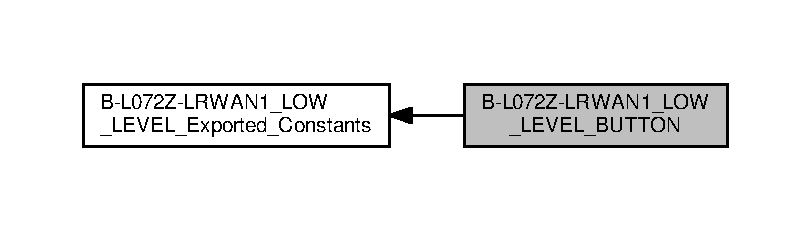
\includegraphics[width=350pt]{group__B-L072Z-LRWAN1__LOW__LEVEL__BUTTON}
\end{center}
\end{figure}
\subsection*{Macros}
\begin{DoxyCompactItemize}
\item 
\#define \hyperlink{group__B-L072Z-LRWAN1__LOW__LEVEL__BUTTON_ga43d47e509ada64329393005c3be15d64}{B\+U\+T\+T\+O\+Nn}~1
\item 
\#define \hyperlink{group__B-L072Z-LRWAN1__LOW__LEVEL__BUTTON_ga34df6915e3013d6a0c74131d3946b659}{U\+S\+E\+R\+\_\+\+B\+U\+T\+T\+O\+N\+\_\+\+P\+IN}~G\+P\+I\+O\+\_\+\+P\+I\+N\+\_\+2
\begin{DoxyCompactList}\small\item\em Key push-\/button. \end{DoxyCompactList}\item 
\#define \hyperlink{group__B-L072Z-LRWAN1__LOW__LEVEL__BUTTON_gae2e6fc2fdfda22b4eed3667375a8bd81}{U\+S\+E\+R\+\_\+\+B\+U\+T\+T\+O\+N\+\_\+\+G\+P\+I\+O\+\_\+\+P\+O\+RT}~G\+P\+I\+OB
\item 
\#define \hyperlink{group__B-L072Z-LRWAN1__LOW__LEVEL__BUTTON_gaa1f35ca26b42710d057661b54ace7d82}{U\+S\+E\+R\+\_\+\+B\+U\+T\+T\+O\+N\+\_\+\+G\+P\+I\+O\+\_\+\+C\+L\+K\+\_\+\+E\+N\+A\+B\+LE}()~\+\_\+\+\_\+\+H\+A\+L\+\_\+\+R\+C\+C\+\_\+\+G\+P\+I\+O\+B\+\_\+\+C\+L\+K\+\_\+\+E\+N\+A\+B\+LE()
\item 
\#define \hyperlink{group__B-L072Z-LRWAN1__LOW__LEVEL__BUTTON_ga71af1d1eec8f8b424b72f625abaad282}{U\+S\+E\+R\+\_\+\+B\+U\+T\+T\+O\+N\+\_\+\+G\+P\+I\+O\+\_\+\+C\+L\+K\+\_\+\+D\+I\+S\+A\+B\+LE}()~\+\_\+\+\_\+\+H\+A\+L\+\_\+\+R\+C\+C\+\_\+\+G\+P\+I\+O\+B\+\_\+\+C\+L\+K\+\_\+\+D\+I\+S\+A\+B\+LE()
\item 
\#define \hyperlink{group__B-L072Z-LRWAN1__LOW__LEVEL__BUTTON_gac41d04c2244ba780e4749991c85d1e9a}{U\+S\+E\+R\+\_\+\+B\+U\+T\+T\+O\+N\+\_\+\+E\+X\+T\+I\+\_\+\+L\+I\+NE}~G\+P\+I\+O\+\_\+\+P\+I\+N\+\_\+2
\item 
\#define \hyperlink{group__B-L072Z-LRWAN1__LOW__LEVEL__BUTTON_ga2e6e65a053529869d1c370610825d98f}{U\+S\+E\+R\+\_\+\+B\+U\+T\+T\+O\+N\+\_\+\+E\+X\+T\+I\+\_\+\+I\+R\+Qn}~E\+X\+T\+I2\+\_\+3\+\_\+\+I\+R\+Qn
\item 
\#define \hyperlink{group__B-L072Z-LRWAN1__LOW__LEVEL__BUTTON_ga5c260a4b4e26836dc3a9b6f15d317421}{K\+E\+Y\+\_\+\+B\+U\+T\+T\+O\+N\+\_\+\+P\+IN}~\hyperlink{group__B-L072Z-LRWAN1__LOW__LEVEL__BUTTON_ga34df6915e3013d6a0c74131d3946b659}{U\+S\+E\+R\+\_\+\+B\+U\+T\+T\+O\+N\+\_\+\+P\+IN}
\item 
\#define \hyperlink{group__B-L072Z-LRWAN1__LOW__LEVEL__BUTTON_ga98680733a6992dacef531bfd0c23031c}{K\+E\+Y\+\_\+\+B\+U\+T\+T\+O\+N\+\_\+\+G\+P\+I\+O\+\_\+\+P\+O\+RT}~\hyperlink{group__B-L072Z-LRWAN1__LOW__LEVEL__BUTTON_gae2e6fc2fdfda22b4eed3667375a8bd81}{U\+S\+E\+R\+\_\+\+B\+U\+T\+T\+O\+N\+\_\+\+G\+P\+I\+O\+\_\+\+P\+O\+RT}
\item 
\#define \hyperlink{group__B-L072Z-LRWAN1__LOW__LEVEL__BUTTON_ga6237d656da42b750f63cbf3e329096d5}{K\+E\+Y\+\_\+\+B\+U\+T\+T\+O\+N\+\_\+\+G\+P\+I\+O\+\_\+\+C\+L\+K\+\_\+\+E\+N\+A\+B\+LE}()~\hyperlink{group__B-L072Z-LRWAN1__LOW__LEVEL__BUTTON_gaa1f35ca26b42710d057661b54ace7d82}{U\+S\+E\+R\+\_\+\+B\+U\+T\+T\+O\+N\+\_\+\+G\+P\+I\+O\+\_\+\+C\+L\+K\+\_\+\+E\+N\+A\+B\+LE}()
\item 
\#define \hyperlink{group__B-L072Z-LRWAN1__LOW__LEVEL__BUTTON_gacf1a6a3b79ec610401d7ffbc1b6115d4}{K\+E\+Y\+\_\+\+B\+U\+T\+T\+O\+N\+\_\+\+G\+P\+I\+O\+\_\+\+C\+L\+K\+\_\+\+D\+I\+S\+A\+B\+LE}()~\hyperlink{group__B-L072Z-LRWAN1__LOW__LEVEL__BUTTON_ga71af1d1eec8f8b424b72f625abaad282}{U\+S\+E\+R\+\_\+\+B\+U\+T\+T\+O\+N\+\_\+\+G\+P\+I\+O\+\_\+\+C\+L\+K\+\_\+\+D\+I\+S\+A\+B\+LE}()
\item 
\#define \hyperlink{group__B-L072Z-LRWAN1__LOW__LEVEL__BUTTON_gae22d60d9f89ae7203bcd5ca8146bcef0}{K\+E\+Y\+\_\+\+B\+U\+T\+T\+O\+N\+\_\+\+E\+X\+T\+I\+\_\+\+L\+I\+NE}~\hyperlink{group__B-L072Z-LRWAN1__LOW__LEVEL__BUTTON_gac41d04c2244ba780e4749991c85d1e9a}{U\+S\+E\+R\+\_\+\+B\+U\+T\+T\+O\+N\+\_\+\+E\+X\+T\+I\+\_\+\+L\+I\+NE}
\item 
\#define \hyperlink{group__B-L072Z-LRWAN1__LOW__LEVEL__BUTTON_gaeb5bffe8281b0754675cfdfb2847e82d}{K\+E\+Y\+\_\+\+B\+U\+T\+T\+O\+N\+\_\+\+E\+X\+T\+I\+\_\+\+I\+R\+Qn}~\hyperlink{group__B-L072Z-LRWAN1__LOW__LEVEL__BUTTON_ga2e6e65a053529869d1c370610825d98f}{U\+S\+E\+R\+\_\+\+B\+U\+T\+T\+O\+N\+\_\+\+E\+X\+T\+I\+\_\+\+I\+R\+Qn}
\item 
\#define \hyperlink{group__B-L072Z-LRWAN1__LOW__LEVEL__BUTTON_gaa397abaece51f4d7aafb07fd79640f3e}{B\+U\+T\+T\+O\+Nx\+\_\+\+G\+P\+I\+O\+\_\+\+C\+L\+K\+\_\+\+E\+N\+A\+B\+LE}(\+\_\+\+\_\+\+I\+N\+D\+E\+X\+\_\+\+\_\+)~do \{\hyperlink{group__B-L072Z-LRWAN1__LOW__LEVEL__BUTTON_ga6237d656da42b750f63cbf3e329096d5}{K\+E\+Y\+\_\+\+B\+U\+T\+T\+O\+N\+\_\+\+G\+P\+I\+O\+\_\+\+C\+L\+K\+\_\+\+E\+N\+A\+B\+LE}();  \} while(0)
\item 
\#define \hyperlink{group__B-L072Z-LRWAN1__LOW__LEVEL__BUTTON_gaf44f31971ce49524d0243b8e37048b8f}{B\+U\+T\+T\+O\+Nx\+\_\+\+G\+P\+I\+O\+\_\+\+C\+L\+K\+\_\+\+D\+I\+S\+A\+B\+LE}(\+\_\+\+\_\+\+I\+N\+D\+E\+X\+\_\+\+\_\+)~do \{K\+E\+Y\+\_\+\+B\+U\+T\+T\+O\+N\+\_\+\+\_\+\+G\+P\+I\+O\+\_\+\+C\+L\+K\+\_\+\+D\+I\+S\+A\+B\+LE();\} while(0)
\end{DoxyCompactItemize}


\subsection{Detailed Description}


\subsection{Macro Definition Documentation}
\mbox{\Hypertarget{group__B-L072Z-LRWAN1__LOW__LEVEL__BUTTON_ga43d47e509ada64329393005c3be15d64}\label{group__B-L072Z-LRWAN1__LOW__LEVEL__BUTTON_ga43d47e509ada64329393005c3be15d64}} 
\index{B-\/\+L072\+Z-\/\+L\+R\+W\+A\+N1\+\_\+\+L\+O\+W\+\_\+\+L\+E\+V\+E\+L\+\_\+\+B\+U\+T\+T\+ON@{B-\/\+L072\+Z-\/\+L\+R\+W\+A\+N1\+\_\+\+L\+O\+W\+\_\+\+L\+E\+V\+E\+L\+\_\+\+B\+U\+T\+T\+ON}!B\+U\+T\+T\+O\+Nn@{B\+U\+T\+T\+O\+Nn}}
\index{B\+U\+T\+T\+O\+Nn@{B\+U\+T\+T\+O\+Nn}!B-\/\+L072\+Z-\/\+L\+R\+W\+A\+N1\+\_\+\+L\+O\+W\+\_\+\+L\+E\+V\+E\+L\+\_\+\+B\+U\+T\+T\+ON@{B-\/\+L072\+Z-\/\+L\+R\+W\+A\+N1\+\_\+\+L\+O\+W\+\_\+\+L\+E\+V\+E\+L\+\_\+\+B\+U\+T\+T\+ON}}
\subsubsection{\texorpdfstring{B\+U\+T\+T\+O\+Nn}{BUTTONn}}
{\footnotesize\ttfamily \#define B\+U\+T\+T\+O\+Nn~1}

\mbox{\Hypertarget{group__B-L072Z-LRWAN1__LOW__LEVEL__BUTTON_gaf44f31971ce49524d0243b8e37048b8f}\label{group__B-L072Z-LRWAN1__LOW__LEVEL__BUTTON_gaf44f31971ce49524d0243b8e37048b8f}} 
\index{B-\/\+L072\+Z-\/\+L\+R\+W\+A\+N1\+\_\+\+L\+O\+W\+\_\+\+L\+E\+V\+E\+L\+\_\+\+B\+U\+T\+T\+ON@{B-\/\+L072\+Z-\/\+L\+R\+W\+A\+N1\+\_\+\+L\+O\+W\+\_\+\+L\+E\+V\+E\+L\+\_\+\+B\+U\+T\+T\+ON}!B\+U\+T\+T\+O\+Nx\+\_\+\+G\+P\+I\+O\+\_\+\+C\+L\+K\+\_\+\+D\+I\+S\+A\+B\+LE@{B\+U\+T\+T\+O\+Nx\+\_\+\+G\+P\+I\+O\+\_\+\+C\+L\+K\+\_\+\+D\+I\+S\+A\+B\+LE}}
\index{B\+U\+T\+T\+O\+Nx\+\_\+\+G\+P\+I\+O\+\_\+\+C\+L\+K\+\_\+\+D\+I\+S\+A\+B\+LE@{B\+U\+T\+T\+O\+Nx\+\_\+\+G\+P\+I\+O\+\_\+\+C\+L\+K\+\_\+\+D\+I\+S\+A\+B\+LE}!B-\/\+L072\+Z-\/\+L\+R\+W\+A\+N1\+\_\+\+L\+O\+W\+\_\+\+L\+E\+V\+E\+L\+\_\+\+B\+U\+T\+T\+ON@{B-\/\+L072\+Z-\/\+L\+R\+W\+A\+N1\+\_\+\+L\+O\+W\+\_\+\+L\+E\+V\+E\+L\+\_\+\+B\+U\+T\+T\+ON}}
\subsubsection{\texorpdfstring{B\+U\+T\+T\+O\+Nx\+\_\+\+G\+P\+I\+O\+\_\+\+C\+L\+K\+\_\+\+D\+I\+S\+A\+B\+LE}{BUTTONx\_GPIO\_CLK\_DISABLE}}
{\footnotesize\ttfamily \#define B\+U\+T\+T\+O\+Nx\+\_\+\+G\+P\+I\+O\+\_\+\+C\+L\+K\+\_\+\+D\+I\+S\+A\+B\+LE(\begin{DoxyParamCaption}\item[{}]{\+\_\+\+\_\+\+I\+N\+D\+E\+X\+\_\+\+\_\+ }\end{DoxyParamCaption})~do \{K\+E\+Y\+\_\+\+B\+U\+T\+T\+O\+N\+\_\+\+\_\+\+G\+P\+I\+O\+\_\+\+C\+L\+K\+\_\+\+D\+I\+S\+A\+B\+LE();\} while(0)}

\mbox{\Hypertarget{group__B-L072Z-LRWAN1__LOW__LEVEL__BUTTON_gaa397abaece51f4d7aafb07fd79640f3e}\label{group__B-L072Z-LRWAN1__LOW__LEVEL__BUTTON_gaa397abaece51f4d7aafb07fd79640f3e}} 
\index{B-\/\+L072\+Z-\/\+L\+R\+W\+A\+N1\+\_\+\+L\+O\+W\+\_\+\+L\+E\+V\+E\+L\+\_\+\+B\+U\+T\+T\+ON@{B-\/\+L072\+Z-\/\+L\+R\+W\+A\+N1\+\_\+\+L\+O\+W\+\_\+\+L\+E\+V\+E\+L\+\_\+\+B\+U\+T\+T\+ON}!B\+U\+T\+T\+O\+Nx\+\_\+\+G\+P\+I\+O\+\_\+\+C\+L\+K\+\_\+\+E\+N\+A\+B\+LE@{B\+U\+T\+T\+O\+Nx\+\_\+\+G\+P\+I\+O\+\_\+\+C\+L\+K\+\_\+\+E\+N\+A\+B\+LE}}
\index{B\+U\+T\+T\+O\+Nx\+\_\+\+G\+P\+I\+O\+\_\+\+C\+L\+K\+\_\+\+E\+N\+A\+B\+LE@{B\+U\+T\+T\+O\+Nx\+\_\+\+G\+P\+I\+O\+\_\+\+C\+L\+K\+\_\+\+E\+N\+A\+B\+LE}!B-\/\+L072\+Z-\/\+L\+R\+W\+A\+N1\+\_\+\+L\+O\+W\+\_\+\+L\+E\+V\+E\+L\+\_\+\+B\+U\+T\+T\+ON@{B-\/\+L072\+Z-\/\+L\+R\+W\+A\+N1\+\_\+\+L\+O\+W\+\_\+\+L\+E\+V\+E\+L\+\_\+\+B\+U\+T\+T\+ON}}
\subsubsection{\texorpdfstring{B\+U\+T\+T\+O\+Nx\+\_\+\+G\+P\+I\+O\+\_\+\+C\+L\+K\+\_\+\+E\+N\+A\+B\+LE}{BUTTONx\_GPIO\_CLK\_ENABLE}}
{\footnotesize\ttfamily \#define B\+U\+T\+T\+O\+Nx\+\_\+\+G\+P\+I\+O\+\_\+\+C\+L\+K\+\_\+\+E\+N\+A\+B\+LE(\begin{DoxyParamCaption}\item[{}]{\+\_\+\+\_\+\+I\+N\+D\+E\+X\+\_\+\+\_\+ }\end{DoxyParamCaption})~do \{\hyperlink{group__B-L072Z-LRWAN1__LOW__LEVEL__BUTTON_ga6237d656da42b750f63cbf3e329096d5}{K\+E\+Y\+\_\+\+B\+U\+T\+T\+O\+N\+\_\+\+G\+P\+I\+O\+\_\+\+C\+L\+K\+\_\+\+E\+N\+A\+B\+LE}();  \} while(0)}

\mbox{\Hypertarget{group__B-L072Z-LRWAN1__LOW__LEVEL__BUTTON_gaeb5bffe8281b0754675cfdfb2847e82d}\label{group__B-L072Z-LRWAN1__LOW__LEVEL__BUTTON_gaeb5bffe8281b0754675cfdfb2847e82d}} 
\index{B-\/\+L072\+Z-\/\+L\+R\+W\+A\+N1\+\_\+\+L\+O\+W\+\_\+\+L\+E\+V\+E\+L\+\_\+\+B\+U\+T\+T\+ON@{B-\/\+L072\+Z-\/\+L\+R\+W\+A\+N1\+\_\+\+L\+O\+W\+\_\+\+L\+E\+V\+E\+L\+\_\+\+B\+U\+T\+T\+ON}!K\+E\+Y\+\_\+\+B\+U\+T\+T\+O\+N\+\_\+\+E\+X\+T\+I\+\_\+\+I\+R\+Qn@{K\+E\+Y\+\_\+\+B\+U\+T\+T\+O\+N\+\_\+\+E\+X\+T\+I\+\_\+\+I\+R\+Qn}}
\index{K\+E\+Y\+\_\+\+B\+U\+T\+T\+O\+N\+\_\+\+E\+X\+T\+I\+\_\+\+I\+R\+Qn@{K\+E\+Y\+\_\+\+B\+U\+T\+T\+O\+N\+\_\+\+E\+X\+T\+I\+\_\+\+I\+R\+Qn}!B-\/\+L072\+Z-\/\+L\+R\+W\+A\+N1\+\_\+\+L\+O\+W\+\_\+\+L\+E\+V\+E\+L\+\_\+\+B\+U\+T\+T\+ON@{B-\/\+L072\+Z-\/\+L\+R\+W\+A\+N1\+\_\+\+L\+O\+W\+\_\+\+L\+E\+V\+E\+L\+\_\+\+B\+U\+T\+T\+ON}}
\subsubsection{\texorpdfstring{K\+E\+Y\+\_\+\+B\+U\+T\+T\+O\+N\+\_\+\+E\+X\+T\+I\+\_\+\+I\+R\+Qn}{KEY\_BUTTON\_EXTI\_IRQn}}
{\footnotesize\ttfamily \#define K\+E\+Y\+\_\+\+B\+U\+T\+T\+O\+N\+\_\+\+E\+X\+T\+I\+\_\+\+I\+R\+Qn~\hyperlink{group__B-L072Z-LRWAN1__LOW__LEVEL__BUTTON_ga2e6e65a053529869d1c370610825d98f}{U\+S\+E\+R\+\_\+\+B\+U\+T\+T\+O\+N\+\_\+\+E\+X\+T\+I\+\_\+\+I\+R\+Qn}}

\mbox{\Hypertarget{group__B-L072Z-LRWAN1__LOW__LEVEL__BUTTON_gae22d60d9f89ae7203bcd5ca8146bcef0}\label{group__B-L072Z-LRWAN1__LOW__LEVEL__BUTTON_gae22d60d9f89ae7203bcd5ca8146bcef0}} 
\index{B-\/\+L072\+Z-\/\+L\+R\+W\+A\+N1\+\_\+\+L\+O\+W\+\_\+\+L\+E\+V\+E\+L\+\_\+\+B\+U\+T\+T\+ON@{B-\/\+L072\+Z-\/\+L\+R\+W\+A\+N1\+\_\+\+L\+O\+W\+\_\+\+L\+E\+V\+E\+L\+\_\+\+B\+U\+T\+T\+ON}!K\+E\+Y\+\_\+\+B\+U\+T\+T\+O\+N\+\_\+\+E\+X\+T\+I\+\_\+\+L\+I\+NE@{K\+E\+Y\+\_\+\+B\+U\+T\+T\+O\+N\+\_\+\+E\+X\+T\+I\+\_\+\+L\+I\+NE}}
\index{K\+E\+Y\+\_\+\+B\+U\+T\+T\+O\+N\+\_\+\+E\+X\+T\+I\+\_\+\+L\+I\+NE@{K\+E\+Y\+\_\+\+B\+U\+T\+T\+O\+N\+\_\+\+E\+X\+T\+I\+\_\+\+L\+I\+NE}!B-\/\+L072\+Z-\/\+L\+R\+W\+A\+N1\+\_\+\+L\+O\+W\+\_\+\+L\+E\+V\+E\+L\+\_\+\+B\+U\+T\+T\+ON@{B-\/\+L072\+Z-\/\+L\+R\+W\+A\+N1\+\_\+\+L\+O\+W\+\_\+\+L\+E\+V\+E\+L\+\_\+\+B\+U\+T\+T\+ON}}
\subsubsection{\texorpdfstring{K\+E\+Y\+\_\+\+B\+U\+T\+T\+O\+N\+\_\+\+E\+X\+T\+I\+\_\+\+L\+I\+NE}{KEY\_BUTTON\_EXTI\_LINE}}
{\footnotesize\ttfamily \#define K\+E\+Y\+\_\+\+B\+U\+T\+T\+O\+N\+\_\+\+E\+X\+T\+I\+\_\+\+L\+I\+NE~\hyperlink{group__B-L072Z-LRWAN1__LOW__LEVEL__BUTTON_gac41d04c2244ba780e4749991c85d1e9a}{U\+S\+E\+R\+\_\+\+B\+U\+T\+T\+O\+N\+\_\+\+E\+X\+T\+I\+\_\+\+L\+I\+NE}}

\mbox{\Hypertarget{group__B-L072Z-LRWAN1__LOW__LEVEL__BUTTON_gacf1a6a3b79ec610401d7ffbc1b6115d4}\label{group__B-L072Z-LRWAN1__LOW__LEVEL__BUTTON_gacf1a6a3b79ec610401d7ffbc1b6115d4}} 
\index{B-\/\+L072\+Z-\/\+L\+R\+W\+A\+N1\+\_\+\+L\+O\+W\+\_\+\+L\+E\+V\+E\+L\+\_\+\+B\+U\+T\+T\+ON@{B-\/\+L072\+Z-\/\+L\+R\+W\+A\+N1\+\_\+\+L\+O\+W\+\_\+\+L\+E\+V\+E\+L\+\_\+\+B\+U\+T\+T\+ON}!K\+E\+Y\+\_\+\+B\+U\+T\+T\+O\+N\+\_\+\+G\+P\+I\+O\+\_\+\+C\+L\+K\+\_\+\+D\+I\+S\+A\+B\+LE@{K\+E\+Y\+\_\+\+B\+U\+T\+T\+O\+N\+\_\+\+G\+P\+I\+O\+\_\+\+C\+L\+K\+\_\+\+D\+I\+S\+A\+B\+LE}}
\index{K\+E\+Y\+\_\+\+B\+U\+T\+T\+O\+N\+\_\+\+G\+P\+I\+O\+\_\+\+C\+L\+K\+\_\+\+D\+I\+S\+A\+B\+LE@{K\+E\+Y\+\_\+\+B\+U\+T\+T\+O\+N\+\_\+\+G\+P\+I\+O\+\_\+\+C\+L\+K\+\_\+\+D\+I\+S\+A\+B\+LE}!B-\/\+L072\+Z-\/\+L\+R\+W\+A\+N1\+\_\+\+L\+O\+W\+\_\+\+L\+E\+V\+E\+L\+\_\+\+B\+U\+T\+T\+ON@{B-\/\+L072\+Z-\/\+L\+R\+W\+A\+N1\+\_\+\+L\+O\+W\+\_\+\+L\+E\+V\+E\+L\+\_\+\+B\+U\+T\+T\+ON}}
\subsubsection{\texorpdfstring{K\+E\+Y\+\_\+\+B\+U\+T\+T\+O\+N\+\_\+\+G\+P\+I\+O\+\_\+\+C\+L\+K\+\_\+\+D\+I\+S\+A\+B\+LE}{KEY\_BUTTON\_GPIO\_CLK\_DISABLE}}
{\footnotesize\ttfamily \#define K\+E\+Y\+\_\+\+B\+U\+T\+T\+O\+N\+\_\+\+G\+P\+I\+O\+\_\+\+C\+L\+K\+\_\+\+D\+I\+S\+A\+B\+LE(\begin{DoxyParamCaption}{ }\end{DoxyParamCaption})~\hyperlink{group__B-L072Z-LRWAN1__LOW__LEVEL__BUTTON_ga71af1d1eec8f8b424b72f625abaad282}{U\+S\+E\+R\+\_\+\+B\+U\+T\+T\+O\+N\+\_\+\+G\+P\+I\+O\+\_\+\+C\+L\+K\+\_\+\+D\+I\+S\+A\+B\+LE}()}

\mbox{\Hypertarget{group__B-L072Z-LRWAN1__LOW__LEVEL__BUTTON_ga6237d656da42b750f63cbf3e329096d5}\label{group__B-L072Z-LRWAN1__LOW__LEVEL__BUTTON_ga6237d656da42b750f63cbf3e329096d5}} 
\index{B-\/\+L072\+Z-\/\+L\+R\+W\+A\+N1\+\_\+\+L\+O\+W\+\_\+\+L\+E\+V\+E\+L\+\_\+\+B\+U\+T\+T\+ON@{B-\/\+L072\+Z-\/\+L\+R\+W\+A\+N1\+\_\+\+L\+O\+W\+\_\+\+L\+E\+V\+E\+L\+\_\+\+B\+U\+T\+T\+ON}!K\+E\+Y\+\_\+\+B\+U\+T\+T\+O\+N\+\_\+\+G\+P\+I\+O\+\_\+\+C\+L\+K\+\_\+\+E\+N\+A\+B\+LE@{K\+E\+Y\+\_\+\+B\+U\+T\+T\+O\+N\+\_\+\+G\+P\+I\+O\+\_\+\+C\+L\+K\+\_\+\+E\+N\+A\+B\+LE}}
\index{K\+E\+Y\+\_\+\+B\+U\+T\+T\+O\+N\+\_\+\+G\+P\+I\+O\+\_\+\+C\+L\+K\+\_\+\+E\+N\+A\+B\+LE@{K\+E\+Y\+\_\+\+B\+U\+T\+T\+O\+N\+\_\+\+G\+P\+I\+O\+\_\+\+C\+L\+K\+\_\+\+E\+N\+A\+B\+LE}!B-\/\+L072\+Z-\/\+L\+R\+W\+A\+N1\+\_\+\+L\+O\+W\+\_\+\+L\+E\+V\+E\+L\+\_\+\+B\+U\+T\+T\+ON@{B-\/\+L072\+Z-\/\+L\+R\+W\+A\+N1\+\_\+\+L\+O\+W\+\_\+\+L\+E\+V\+E\+L\+\_\+\+B\+U\+T\+T\+ON}}
\subsubsection{\texorpdfstring{K\+E\+Y\+\_\+\+B\+U\+T\+T\+O\+N\+\_\+\+G\+P\+I\+O\+\_\+\+C\+L\+K\+\_\+\+E\+N\+A\+B\+LE}{KEY\_BUTTON\_GPIO\_CLK\_ENABLE}}
{\footnotesize\ttfamily \#define K\+E\+Y\+\_\+\+B\+U\+T\+T\+O\+N\+\_\+\+G\+P\+I\+O\+\_\+\+C\+L\+K\+\_\+\+E\+N\+A\+B\+LE(\begin{DoxyParamCaption}{ }\end{DoxyParamCaption})~\hyperlink{group__B-L072Z-LRWAN1__LOW__LEVEL__BUTTON_gaa1f35ca26b42710d057661b54ace7d82}{U\+S\+E\+R\+\_\+\+B\+U\+T\+T\+O\+N\+\_\+\+G\+P\+I\+O\+\_\+\+C\+L\+K\+\_\+\+E\+N\+A\+B\+LE}()}

\mbox{\Hypertarget{group__B-L072Z-LRWAN1__LOW__LEVEL__BUTTON_ga98680733a6992dacef531bfd0c23031c}\label{group__B-L072Z-LRWAN1__LOW__LEVEL__BUTTON_ga98680733a6992dacef531bfd0c23031c}} 
\index{B-\/\+L072\+Z-\/\+L\+R\+W\+A\+N1\+\_\+\+L\+O\+W\+\_\+\+L\+E\+V\+E\+L\+\_\+\+B\+U\+T\+T\+ON@{B-\/\+L072\+Z-\/\+L\+R\+W\+A\+N1\+\_\+\+L\+O\+W\+\_\+\+L\+E\+V\+E\+L\+\_\+\+B\+U\+T\+T\+ON}!K\+E\+Y\+\_\+\+B\+U\+T\+T\+O\+N\+\_\+\+G\+P\+I\+O\+\_\+\+P\+O\+RT@{K\+E\+Y\+\_\+\+B\+U\+T\+T\+O\+N\+\_\+\+G\+P\+I\+O\+\_\+\+P\+O\+RT}}
\index{K\+E\+Y\+\_\+\+B\+U\+T\+T\+O\+N\+\_\+\+G\+P\+I\+O\+\_\+\+P\+O\+RT@{K\+E\+Y\+\_\+\+B\+U\+T\+T\+O\+N\+\_\+\+G\+P\+I\+O\+\_\+\+P\+O\+RT}!B-\/\+L072\+Z-\/\+L\+R\+W\+A\+N1\+\_\+\+L\+O\+W\+\_\+\+L\+E\+V\+E\+L\+\_\+\+B\+U\+T\+T\+ON@{B-\/\+L072\+Z-\/\+L\+R\+W\+A\+N1\+\_\+\+L\+O\+W\+\_\+\+L\+E\+V\+E\+L\+\_\+\+B\+U\+T\+T\+ON}}
\subsubsection{\texorpdfstring{K\+E\+Y\+\_\+\+B\+U\+T\+T\+O\+N\+\_\+\+G\+P\+I\+O\+\_\+\+P\+O\+RT}{KEY\_BUTTON\_GPIO\_PORT}}
{\footnotesize\ttfamily \#define K\+E\+Y\+\_\+\+B\+U\+T\+T\+O\+N\+\_\+\+G\+P\+I\+O\+\_\+\+P\+O\+RT~\hyperlink{group__B-L072Z-LRWAN1__LOW__LEVEL__BUTTON_gae2e6fc2fdfda22b4eed3667375a8bd81}{U\+S\+E\+R\+\_\+\+B\+U\+T\+T\+O\+N\+\_\+\+G\+P\+I\+O\+\_\+\+P\+O\+RT}}

\mbox{\Hypertarget{group__B-L072Z-LRWAN1__LOW__LEVEL__BUTTON_ga5c260a4b4e26836dc3a9b6f15d317421}\label{group__B-L072Z-LRWAN1__LOW__LEVEL__BUTTON_ga5c260a4b4e26836dc3a9b6f15d317421}} 
\index{B-\/\+L072\+Z-\/\+L\+R\+W\+A\+N1\+\_\+\+L\+O\+W\+\_\+\+L\+E\+V\+E\+L\+\_\+\+B\+U\+T\+T\+ON@{B-\/\+L072\+Z-\/\+L\+R\+W\+A\+N1\+\_\+\+L\+O\+W\+\_\+\+L\+E\+V\+E\+L\+\_\+\+B\+U\+T\+T\+ON}!K\+E\+Y\+\_\+\+B\+U\+T\+T\+O\+N\+\_\+\+P\+IN@{K\+E\+Y\+\_\+\+B\+U\+T\+T\+O\+N\+\_\+\+P\+IN}}
\index{K\+E\+Y\+\_\+\+B\+U\+T\+T\+O\+N\+\_\+\+P\+IN@{K\+E\+Y\+\_\+\+B\+U\+T\+T\+O\+N\+\_\+\+P\+IN}!B-\/\+L072\+Z-\/\+L\+R\+W\+A\+N1\+\_\+\+L\+O\+W\+\_\+\+L\+E\+V\+E\+L\+\_\+\+B\+U\+T\+T\+ON@{B-\/\+L072\+Z-\/\+L\+R\+W\+A\+N1\+\_\+\+L\+O\+W\+\_\+\+L\+E\+V\+E\+L\+\_\+\+B\+U\+T\+T\+ON}}
\subsubsection{\texorpdfstring{K\+E\+Y\+\_\+\+B\+U\+T\+T\+O\+N\+\_\+\+P\+IN}{KEY\_BUTTON\_PIN}}
{\footnotesize\ttfamily \#define K\+E\+Y\+\_\+\+B\+U\+T\+T\+O\+N\+\_\+\+P\+IN~\hyperlink{group__B-L072Z-LRWAN1__LOW__LEVEL__BUTTON_ga34df6915e3013d6a0c74131d3946b659}{U\+S\+E\+R\+\_\+\+B\+U\+T\+T\+O\+N\+\_\+\+P\+IN}}

\mbox{\Hypertarget{group__B-L072Z-LRWAN1__LOW__LEVEL__BUTTON_ga2e6e65a053529869d1c370610825d98f}\label{group__B-L072Z-LRWAN1__LOW__LEVEL__BUTTON_ga2e6e65a053529869d1c370610825d98f}} 
\index{B-\/\+L072\+Z-\/\+L\+R\+W\+A\+N1\+\_\+\+L\+O\+W\+\_\+\+L\+E\+V\+E\+L\+\_\+\+B\+U\+T\+T\+ON@{B-\/\+L072\+Z-\/\+L\+R\+W\+A\+N1\+\_\+\+L\+O\+W\+\_\+\+L\+E\+V\+E\+L\+\_\+\+B\+U\+T\+T\+ON}!U\+S\+E\+R\+\_\+\+B\+U\+T\+T\+O\+N\+\_\+\+E\+X\+T\+I\+\_\+\+I\+R\+Qn@{U\+S\+E\+R\+\_\+\+B\+U\+T\+T\+O\+N\+\_\+\+E\+X\+T\+I\+\_\+\+I\+R\+Qn}}
\index{U\+S\+E\+R\+\_\+\+B\+U\+T\+T\+O\+N\+\_\+\+E\+X\+T\+I\+\_\+\+I\+R\+Qn@{U\+S\+E\+R\+\_\+\+B\+U\+T\+T\+O\+N\+\_\+\+E\+X\+T\+I\+\_\+\+I\+R\+Qn}!B-\/\+L072\+Z-\/\+L\+R\+W\+A\+N1\+\_\+\+L\+O\+W\+\_\+\+L\+E\+V\+E\+L\+\_\+\+B\+U\+T\+T\+ON@{B-\/\+L072\+Z-\/\+L\+R\+W\+A\+N1\+\_\+\+L\+O\+W\+\_\+\+L\+E\+V\+E\+L\+\_\+\+B\+U\+T\+T\+ON}}
\subsubsection{\texorpdfstring{U\+S\+E\+R\+\_\+\+B\+U\+T\+T\+O\+N\+\_\+\+E\+X\+T\+I\+\_\+\+I\+R\+Qn}{USER\_BUTTON\_EXTI\_IRQn}}
{\footnotesize\ttfamily \#define U\+S\+E\+R\+\_\+\+B\+U\+T\+T\+O\+N\+\_\+\+E\+X\+T\+I\+\_\+\+I\+R\+Qn~E\+X\+T\+I2\+\_\+3\+\_\+\+I\+R\+Qn}

\mbox{\Hypertarget{group__B-L072Z-LRWAN1__LOW__LEVEL__BUTTON_gac41d04c2244ba780e4749991c85d1e9a}\label{group__B-L072Z-LRWAN1__LOW__LEVEL__BUTTON_gac41d04c2244ba780e4749991c85d1e9a}} 
\index{B-\/\+L072\+Z-\/\+L\+R\+W\+A\+N1\+\_\+\+L\+O\+W\+\_\+\+L\+E\+V\+E\+L\+\_\+\+B\+U\+T\+T\+ON@{B-\/\+L072\+Z-\/\+L\+R\+W\+A\+N1\+\_\+\+L\+O\+W\+\_\+\+L\+E\+V\+E\+L\+\_\+\+B\+U\+T\+T\+ON}!U\+S\+E\+R\+\_\+\+B\+U\+T\+T\+O\+N\+\_\+\+E\+X\+T\+I\+\_\+\+L\+I\+NE@{U\+S\+E\+R\+\_\+\+B\+U\+T\+T\+O\+N\+\_\+\+E\+X\+T\+I\+\_\+\+L\+I\+NE}}
\index{U\+S\+E\+R\+\_\+\+B\+U\+T\+T\+O\+N\+\_\+\+E\+X\+T\+I\+\_\+\+L\+I\+NE@{U\+S\+E\+R\+\_\+\+B\+U\+T\+T\+O\+N\+\_\+\+E\+X\+T\+I\+\_\+\+L\+I\+NE}!B-\/\+L072\+Z-\/\+L\+R\+W\+A\+N1\+\_\+\+L\+O\+W\+\_\+\+L\+E\+V\+E\+L\+\_\+\+B\+U\+T\+T\+ON@{B-\/\+L072\+Z-\/\+L\+R\+W\+A\+N1\+\_\+\+L\+O\+W\+\_\+\+L\+E\+V\+E\+L\+\_\+\+B\+U\+T\+T\+ON}}
\subsubsection{\texorpdfstring{U\+S\+E\+R\+\_\+\+B\+U\+T\+T\+O\+N\+\_\+\+E\+X\+T\+I\+\_\+\+L\+I\+NE}{USER\_BUTTON\_EXTI\_LINE}}
{\footnotesize\ttfamily \#define U\+S\+E\+R\+\_\+\+B\+U\+T\+T\+O\+N\+\_\+\+E\+X\+T\+I\+\_\+\+L\+I\+NE~G\+P\+I\+O\+\_\+\+P\+I\+N\+\_\+2}

\mbox{\Hypertarget{group__B-L072Z-LRWAN1__LOW__LEVEL__BUTTON_ga71af1d1eec8f8b424b72f625abaad282}\label{group__B-L072Z-LRWAN1__LOW__LEVEL__BUTTON_ga71af1d1eec8f8b424b72f625abaad282}} 
\index{B-\/\+L072\+Z-\/\+L\+R\+W\+A\+N1\+\_\+\+L\+O\+W\+\_\+\+L\+E\+V\+E\+L\+\_\+\+B\+U\+T\+T\+ON@{B-\/\+L072\+Z-\/\+L\+R\+W\+A\+N1\+\_\+\+L\+O\+W\+\_\+\+L\+E\+V\+E\+L\+\_\+\+B\+U\+T\+T\+ON}!U\+S\+E\+R\+\_\+\+B\+U\+T\+T\+O\+N\+\_\+\+G\+P\+I\+O\+\_\+\+C\+L\+K\+\_\+\+D\+I\+S\+A\+B\+LE@{U\+S\+E\+R\+\_\+\+B\+U\+T\+T\+O\+N\+\_\+\+G\+P\+I\+O\+\_\+\+C\+L\+K\+\_\+\+D\+I\+S\+A\+B\+LE}}
\index{U\+S\+E\+R\+\_\+\+B\+U\+T\+T\+O\+N\+\_\+\+G\+P\+I\+O\+\_\+\+C\+L\+K\+\_\+\+D\+I\+S\+A\+B\+LE@{U\+S\+E\+R\+\_\+\+B\+U\+T\+T\+O\+N\+\_\+\+G\+P\+I\+O\+\_\+\+C\+L\+K\+\_\+\+D\+I\+S\+A\+B\+LE}!B-\/\+L072\+Z-\/\+L\+R\+W\+A\+N1\+\_\+\+L\+O\+W\+\_\+\+L\+E\+V\+E\+L\+\_\+\+B\+U\+T\+T\+ON@{B-\/\+L072\+Z-\/\+L\+R\+W\+A\+N1\+\_\+\+L\+O\+W\+\_\+\+L\+E\+V\+E\+L\+\_\+\+B\+U\+T\+T\+ON}}
\subsubsection{\texorpdfstring{U\+S\+E\+R\+\_\+\+B\+U\+T\+T\+O\+N\+\_\+\+G\+P\+I\+O\+\_\+\+C\+L\+K\+\_\+\+D\+I\+S\+A\+B\+LE}{USER\_BUTTON\_GPIO\_CLK\_DISABLE}}
{\footnotesize\ttfamily \#define U\+S\+E\+R\+\_\+\+B\+U\+T\+T\+O\+N\+\_\+\+G\+P\+I\+O\+\_\+\+C\+L\+K\+\_\+\+D\+I\+S\+A\+B\+LE(\begin{DoxyParamCaption}{ }\end{DoxyParamCaption})~\+\_\+\+\_\+\+H\+A\+L\+\_\+\+R\+C\+C\+\_\+\+G\+P\+I\+O\+B\+\_\+\+C\+L\+K\+\_\+\+D\+I\+S\+A\+B\+LE()}

\mbox{\Hypertarget{group__B-L072Z-LRWAN1__LOW__LEVEL__BUTTON_gaa1f35ca26b42710d057661b54ace7d82}\label{group__B-L072Z-LRWAN1__LOW__LEVEL__BUTTON_gaa1f35ca26b42710d057661b54ace7d82}} 
\index{B-\/\+L072\+Z-\/\+L\+R\+W\+A\+N1\+\_\+\+L\+O\+W\+\_\+\+L\+E\+V\+E\+L\+\_\+\+B\+U\+T\+T\+ON@{B-\/\+L072\+Z-\/\+L\+R\+W\+A\+N1\+\_\+\+L\+O\+W\+\_\+\+L\+E\+V\+E\+L\+\_\+\+B\+U\+T\+T\+ON}!U\+S\+E\+R\+\_\+\+B\+U\+T\+T\+O\+N\+\_\+\+G\+P\+I\+O\+\_\+\+C\+L\+K\+\_\+\+E\+N\+A\+B\+LE@{U\+S\+E\+R\+\_\+\+B\+U\+T\+T\+O\+N\+\_\+\+G\+P\+I\+O\+\_\+\+C\+L\+K\+\_\+\+E\+N\+A\+B\+LE}}
\index{U\+S\+E\+R\+\_\+\+B\+U\+T\+T\+O\+N\+\_\+\+G\+P\+I\+O\+\_\+\+C\+L\+K\+\_\+\+E\+N\+A\+B\+LE@{U\+S\+E\+R\+\_\+\+B\+U\+T\+T\+O\+N\+\_\+\+G\+P\+I\+O\+\_\+\+C\+L\+K\+\_\+\+E\+N\+A\+B\+LE}!B-\/\+L072\+Z-\/\+L\+R\+W\+A\+N1\+\_\+\+L\+O\+W\+\_\+\+L\+E\+V\+E\+L\+\_\+\+B\+U\+T\+T\+ON@{B-\/\+L072\+Z-\/\+L\+R\+W\+A\+N1\+\_\+\+L\+O\+W\+\_\+\+L\+E\+V\+E\+L\+\_\+\+B\+U\+T\+T\+ON}}
\subsubsection{\texorpdfstring{U\+S\+E\+R\+\_\+\+B\+U\+T\+T\+O\+N\+\_\+\+G\+P\+I\+O\+\_\+\+C\+L\+K\+\_\+\+E\+N\+A\+B\+LE}{USER\_BUTTON\_GPIO\_CLK\_ENABLE}}
{\footnotesize\ttfamily \#define U\+S\+E\+R\+\_\+\+B\+U\+T\+T\+O\+N\+\_\+\+G\+P\+I\+O\+\_\+\+C\+L\+K\+\_\+\+E\+N\+A\+B\+LE(\begin{DoxyParamCaption}{ }\end{DoxyParamCaption})~\+\_\+\+\_\+\+H\+A\+L\+\_\+\+R\+C\+C\+\_\+\+G\+P\+I\+O\+B\+\_\+\+C\+L\+K\+\_\+\+E\+N\+A\+B\+LE()}

\mbox{\Hypertarget{group__B-L072Z-LRWAN1__LOW__LEVEL__BUTTON_gae2e6fc2fdfda22b4eed3667375a8bd81}\label{group__B-L072Z-LRWAN1__LOW__LEVEL__BUTTON_gae2e6fc2fdfda22b4eed3667375a8bd81}} 
\index{B-\/\+L072\+Z-\/\+L\+R\+W\+A\+N1\+\_\+\+L\+O\+W\+\_\+\+L\+E\+V\+E\+L\+\_\+\+B\+U\+T\+T\+ON@{B-\/\+L072\+Z-\/\+L\+R\+W\+A\+N1\+\_\+\+L\+O\+W\+\_\+\+L\+E\+V\+E\+L\+\_\+\+B\+U\+T\+T\+ON}!U\+S\+E\+R\+\_\+\+B\+U\+T\+T\+O\+N\+\_\+\+G\+P\+I\+O\+\_\+\+P\+O\+RT@{U\+S\+E\+R\+\_\+\+B\+U\+T\+T\+O\+N\+\_\+\+G\+P\+I\+O\+\_\+\+P\+O\+RT}}
\index{U\+S\+E\+R\+\_\+\+B\+U\+T\+T\+O\+N\+\_\+\+G\+P\+I\+O\+\_\+\+P\+O\+RT@{U\+S\+E\+R\+\_\+\+B\+U\+T\+T\+O\+N\+\_\+\+G\+P\+I\+O\+\_\+\+P\+O\+RT}!B-\/\+L072\+Z-\/\+L\+R\+W\+A\+N1\+\_\+\+L\+O\+W\+\_\+\+L\+E\+V\+E\+L\+\_\+\+B\+U\+T\+T\+ON@{B-\/\+L072\+Z-\/\+L\+R\+W\+A\+N1\+\_\+\+L\+O\+W\+\_\+\+L\+E\+V\+E\+L\+\_\+\+B\+U\+T\+T\+ON}}
\subsubsection{\texorpdfstring{U\+S\+E\+R\+\_\+\+B\+U\+T\+T\+O\+N\+\_\+\+G\+P\+I\+O\+\_\+\+P\+O\+RT}{USER\_BUTTON\_GPIO\_PORT}}
{\footnotesize\ttfamily \#define U\+S\+E\+R\+\_\+\+B\+U\+T\+T\+O\+N\+\_\+\+G\+P\+I\+O\+\_\+\+P\+O\+RT~G\+P\+I\+OB}

\mbox{\Hypertarget{group__B-L072Z-LRWAN1__LOW__LEVEL__BUTTON_ga34df6915e3013d6a0c74131d3946b659}\label{group__B-L072Z-LRWAN1__LOW__LEVEL__BUTTON_ga34df6915e3013d6a0c74131d3946b659}} 
\index{B-\/\+L072\+Z-\/\+L\+R\+W\+A\+N1\+\_\+\+L\+O\+W\+\_\+\+L\+E\+V\+E\+L\+\_\+\+B\+U\+T\+T\+ON@{B-\/\+L072\+Z-\/\+L\+R\+W\+A\+N1\+\_\+\+L\+O\+W\+\_\+\+L\+E\+V\+E\+L\+\_\+\+B\+U\+T\+T\+ON}!U\+S\+E\+R\+\_\+\+B\+U\+T\+T\+O\+N\+\_\+\+P\+IN@{U\+S\+E\+R\+\_\+\+B\+U\+T\+T\+O\+N\+\_\+\+P\+IN}}
\index{U\+S\+E\+R\+\_\+\+B\+U\+T\+T\+O\+N\+\_\+\+P\+IN@{U\+S\+E\+R\+\_\+\+B\+U\+T\+T\+O\+N\+\_\+\+P\+IN}!B-\/\+L072\+Z-\/\+L\+R\+W\+A\+N1\+\_\+\+L\+O\+W\+\_\+\+L\+E\+V\+E\+L\+\_\+\+B\+U\+T\+T\+ON@{B-\/\+L072\+Z-\/\+L\+R\+W\+A\+N1\+\_\+\+L\+O\+W\+\_\+\+L\+E\+V\+E\+L\+\_\+\+B\+U\+T\+T\+ON}}
\subsubsection{\texorpdfstring{U\+S\+E\+R\+\_\+\+B\+U\+T\+T\+O\+N\+\_\+\+P\+IN}{USER\_BUTTON\_PIN}}
{\footnotesize\ttfamily \#define U\+S\+E\+R\+\_\+\+B\+U\+T\+T\+O\+N\+\_\+\+P\+IN~G\+P\+I\+O\+\_\+\+P\+I\+N\+\_\+2}



Key push-\/button. 


\chapter{Data Structure Documentation}
\hypertarget{structFskBandwidth__t}{}\section{Fsk\+Bandwidth\+\_\+t Struct Reference}
\label{structFskBandwidth__t}\index{Fsk\+Bandwidth\+\_\+t@{Fsk\+Bandwidth\+\_\+t}}
\subsection*{Data Fields}
\begin{DoxyCompactItemize}
\item 
uint32\+\_\+t \hyperlink{structFskBandwidth__t_a717a088404f8ffffb01286095ed8a553}{bandwidth}
\item 
uint8\+\_\+t \hyperlink{structFskBandwidth__t_ac401e2f55f51b74911db229b1644de87}{Reg\+Value}
\end{DoxyCompactItemize}


\subsection{Detailed Description}
F\+SK bandwidth definition 

\subsection{Field Documentation}
\mbox{\Hypertarget{structFskBandwidth__t_a717a088404f8ffffb01286095ed8a553}\label{structFskBandwidth__t_a717a088404f8ffffb01286095ed8a553}} 
\index{Fsk\+Bandwidth\+\_\+t@{Fsk\+Bandwidth\+\_\+t}!bandwidth@{bandwidth}}
\index{bandwidth@{bandwidth}!Fsk\+Bandwidth\+\_\+t@{Fsk\+Bandwidth\+\_\+t}}
\subsubsection{\texorpdfstring{bandwidth}{bandwidth}}
{\footnotesize\ttfamily uint32\+\_\+t Fsk\+Bandwidth\+\_\+t\+::bandwidth}

\mbox{\Hypertarget{structFskBandwidth__t_ac401e2f55f51b74911db229b1644de87}\label{structFskBandwidth__t_ac401e2f55f51b74911db229b1644de87}} 
\index{Fsk\+Bandwidth\+\_\+t@{Fsk\+Bandwidth\+\_\+t}!Reg\+Value@{Reg\+Value}}
\index{Reg\+Value@{Reg\+Value}!Fsk\+Bandwidth\+\_\+t@{Fsk\+Bandwidth\+\_\+t}}
\subsubsection{\texorpdfstring{Reg\+Value}{RegValue}}
{\footnotesize\ttfamily uint8\+\_\+t Fsk\+Bandwidth\+\_\+t\+::\+Reg\+Value}



The documentation for this struct was generated from the following file\+:\begin{DoxyCompactItemize}
\item 
Components/sx1276/\hyperlink{sx1276_8c}{sx1276.\+c}\end{DoxyCompactItemize}

\hypertarget{structRadioFskPacketHandler__t}{}\section{Radio\+Fsk\+Packet\+Handler\+\_\+t Struct Reference}
\label{structRadioFskPacketHandler__t}\index{Radio\+Fsk\+Packet\+Handler\+\_\+t@{Radio\+Fsk\+Packet\+Handler\+\_\+t}}


{\ttfamily \#include $<$sx1276.\+h$>$}

\subsection*{Data Fields}
\begin{DoxyCompactItemize}
\item 
uint8\+\_\+t \hyperlink{structRadioFskPacketHandler__t_a97c923759975964c814a1242a9066cf4}{Preamble\+Detected}
\item 
uint8\+\_\+t \hyperlink{structRadioFskPacketHandler__t_aeaa0cefa4c67703953b8cf9ee2bf74cc}{Sync\+Word\+Detected}
\item 
int8\+\_\+t \hyperlink{structRadioFskPacketHandler__t_ac8c8c5d7a472439647c7191bdc08d018}{Rssi\+Value}
\item 
int32\+\_\+t \hyperlink{structRadioFskPacketHandler__t_ae4ba7d5bae19bb4e544986c6f518a583}{Afc\+Value}
\item 
uint8\+\_\+t \hyperlink{structRadioFskPacketHandler__t_a88f8201830b4db2d710542057a9697f6}{Rx\+Gain}
\item 
uint16\+\_\+t \hyperlink{structRadioFskPacketHandler__t_ada3d579022ff861f2039bf506a5b9ca2}{Size}
\item 
uint16\+\_\+t \hyperlink{structRadioFskPacketHandler__t_abc3c832c34dcbc8511aab189c2e752f1}{Nb\+Bytes}
\item 
uint8\+\_\+t \hyperlink{structRadioFskPacketHandler__t_aa5d2d8ab8dd126a3d46bddfc1cf2df92}{Fifo\+Thresh}
\item 
uint8\+\_\+t \hyperlink{structRadioFskPacketHandler__t_ade09fc9f108fa6ff8cfc3180d9094cb8}{Chunk\+Size}
\end{DoxyCompactItemize}


\subsection{Detailed Description}
Radio F\+SK packet handler state 

\subsection{Field Documentation}
\mbox{\Hypertarget{structRadioFskPacketHandler__t_ae4ba7d5bae19bb4e544986c6f518a583}\label{structRadioFskPacketHandler__t_ae4ba7d5bae19bb4e544986c6f518a583}} 
\index{Radio\+Fsk\+Packet\+Handler\+\_\+t@{Radio\+Fsk\+Packet\+Handler\+\_\+t}!Afc\+Value@{Afc\+Value}}
\index{Afc\+Value@{Afc\+Value}!Radio\+Fsk\+Packet\+Handler\+\_\+t@{Radio\+Fsk\+Packet\+Handler\+\_\+t}}
\subsubsection{\texorpdfstring{Afc\+Value}{AfcValue}}
{\footnotesize\ttfamily int32\+\_\+t Radio\+Fsk\+Packet\+Handler\+\_\+t\+::\+Afc\+Value}

\mbox{\Hypertarget{structRadioFskPacketHandler__t_ade09fc9f108fa6ff8cfc3180d9094cb8}\label{structRadioFskPacketHandler__t_ade09fc9f108fa6ff8cfc3180d9094cb8}} 
\index{Radio\+Fsk\+Packet\+Handler\+\_\+t@{Radio\+Fsk\+Packet\+Handler\+\_\+t}!Chunk\+Size@{Chunk\+Size}}
\index{Chunk\+Size@{Chunk\+Size}!Radio\+Fsk\+Packet\+Handler\+\_\+t@{Radio\+Fsk\+Packet\+Handler\+\_\+t}}
\subsubsection{\texorpdfstring{Chunk\+Size}{ChunkSize}}
{\footnotesize\ttfamily uint8\+\_\+t Radio\+Fsk\+Packet\+Handler\+\_\+t\+::\+Chunk\+Size}

\mbox{\Hypertarget{structRadioFskPacketHandler__t_aa5d2d8ab8dd126a3d46bddfc1cf2df92}\label{structRadioFskPacketHandler__t_aa5d2d8ab8dd126a3d46bddfc1cf2df92}} 
\index{Radio\+Fsk\+Packet\+Handler\+\_\+t@{Radio\+Fsk\+Packet\+Handler\+\_\+t}!Fifo\+Thresh@{Fifo\+Thresh}}
\index{Fifo\+Thresh@{Fifo\+Thresh}!Radio\+Fsk\+Packet\+Handler\+\_\+t@{Radio\+Fsk\+Packet\+Handler\+\_\+t}}
\subsubsection{\texorpdfstring{Fifo\+Thresh}{FifoThresh}}
{\footnotesize\ttfamily uint8\+\_\+t Radio\+Fsk\+Packet\+Handler\+\_\+t\+::\+Fifo\+Thresh}

\mbox{\Hypertarget{structRadioFskPacketHandler__t_abc3c832c34dcbc8511aab189c2e752f1}\label{structRadioFskPacketHandler__t_abc3c832c34dcbc8511aab189c2e752f1}} 
\index{Radio\+Fsk\+Packet\+Handler\+\_\+t@{Radio\+Fsk\+Packet\+Handler\+\_\+t}!Nb\+Bytes@{Nb\+Bytes}}
\index{Nb\+Bytes@{Nb\+Bytes}!Radio\+Fsk\+Packet\+Handler\+\_\+t@{Radio\+Fsk\+Packet\+Handler\+\_\+t}}
\subsubsection{\texorpdfstring{Nb\+Bytes}{NbBytes}}
{\footnotesize\ttfamily uint16\+\_\+t Radio\+Fsk\+Packet\+Handler\+\_\+t\+::\+Nb\+Bytes}

\mbox{\Hypertarget{structRadioFskPacketHandler__t_a97c923759975964c814a1242a9066cf4}\label{structRadioFskPacketHandler__t_a97c923759975964c814a1242a9066cf4}} 
\index{Radio\+Fsk\+Packet\+Handler\+\_\+t@{Radio\+Fsk\+Packet\+Handler\+\_\+t}!Preamble\+Detected@{Preamble\+Detected}}
\index{Preamble\+Detected@{Preamble\+Detected}!Radio\+Fsk\+Packet\+Handler\+\_\+t@{Radio\+Fsk\+Packet\+Handler\+\_\+t}}
\subsubsection{\texorpdfstring{Preamble\+Detected}{PreambleDetected}}
{\footnotesize\ttfamily uint8\+\_\+t Radio\+Fsk\+Packet\+Handler\+\_\+t\+::\+Preamble\+Detected}

\mbox{\Hypertarget{structRadioFskPacketHandler__t_ac8c8c5d7a472439647c7191bdc08d018}\label{structRadioFskPacketHandler__t_ac8c8c5d7a472439647c7191bdc08d018}} 
\index{Radio\+Fsk\+Packet\+Handler\+\_\+t@{Radio\+Fsk\+Packet\+Handler\+\_\+t}!Rssi\+Value@{Rssi\+Value}}
\index{Rssi\+Value@{Rssi\+Value}!Radio\+Fsk\+Packet\+Handler\+\_\+t@{Radio\+Fsk\+Packet\+Handler\+\_\+t}}
\subsubsection{\texorpdfstring{Rssi\+Value}{RssiValue}}
{\footnotesize\ttfamily int8\+\_\+t Radio\+Fsk\+Packet\+Handler\+\_\+t\+::\+Rssi\+Value}

\mbox{\Hypertarget{structRadioFskPacketHandler__t_a88f8201830b4db2d710542057a9697f6}\label{structRadioFskPacketHandler__t_a88f8201830b4db2d710542057a9697f6}} 
\index{Radio\+Fsk\+Packet\+Handler\+\_\+t@{Radio\+Fsk\+Packet\+Handler\+\_\+t}!Rx\+Gain@{Rx\+Gain}}
\index{Rx\+Gain@{Rx\+Gain}!Radio\+Fsk\+Packet\+Handler\+\_\+t@{Radio\+Fsk\+Packet\+Handler\+\_\+t}}
\subsubsection{\texorpdfstring{Rx\+Gain}{RxGain}}
{\footnotesize\ttfamily uint8\+\_\+t Radio\+Fsk\+Packet\+Handler\+\_\+t\+::\+Rx\+Gain}

\mbox{\Hypertarget{structRadioFskPacketHandler__t_ada3d579022ff861f2039bf506a5b9ca2}\label{structRadioFskPacketHandler__t_ada3d579022ff861f2039bf506a5b9ca2}} 
\index{Radio\+Fsk\+Packet\+Handler\+\_\+t@{Radio\+Fsk\+Packet\+Handler\+\_\+t}!Size@{Size}}
\index{Size@{Size}!Radio\+Fsk\+Packet\+Handler\+\_\+t@{Radio\+Fsk\+Packet\+Handler\+\_\+t}}
\subsubsection{\texorpdfstring{Size}{Size}}
{\footnotesize\ttfamily uint16\+\_\+t Radio\+Fsk\+Packet\+Handler\+\_\+t\+::\+Size}

\mbox{\Hypertarget{structRadioFskPacketHandler__t_aeaa0cefa4c67703953b8cf9ee2bf74cc}\label{structRadioFskPacketHandler__t_aeaa0cefa4c67703953b8cf9ee2bf74cc}} 
\index{Radio\+Fsk\+Packet\+Handler\+\_\+t@{Radio\+Fsk\+Packet\+Handler\+\_\+t}!Sync\+Word\+Detected@{Sync\+Word\+Detected}}
\index{Sync\+Word\+Detected@{Sync\+Word\+Detected}!Radio\+Fsk\+Packet\+Handler\+\_\+t@{Radio\+Fsk\+Packet\+Handler\+\_\+t}}
\subsubsection{\texorpdfstring{Sync\+Word\+Detected}{SyncWordDetected}}
{\footnotesize\ttfamily uint8\+\_\+t Radio\+Fsk\+Packet\+Handler\+\_\+t\+::\+Sync\+Word\+Detected}



The documentation for this struct was generated from the following file\+:\begin{DoxyCompactItemize}
\item 
Components/sx1276/\hyperlink{sx1276_8h}{sx1276.\+h}\end{DoxyCompactItemize}

\hypertarget{structRadioFskSettings__t}{}\section{Radio\+Fsk\+Settings\+\_\+t Struct Reference}
\label{structRadioFskSettings__t}\index{Radio\+Fsk\+Settings\+\_\+t@{Radio\+Fsk\+Settings\+\_\+t}}


{\ttfamily \#include $<$sx1276.\+h$>$}

\subsection*{Data Fields}
\begin{DoxyCompactItemize}
\item 
int8\+\_\+t \hyperlink{structRadioFskSettings__t_ab149ce9b6cef37f6d06cc9196af0c4fc}{Power}
\item 
uint32\+\_\+t \hyperlink{structRadioFskSettings__t_ad3848ad0938d9668710ff78b0f3ee36f}{Fdev}
\item 
uint32\+\_\+t \hyperlink{structRadioFskSettings__t_a357f643a26a7a073a1ef9e202aa06923}{Bandwidth}
\item 
uint32\+\_\+t \hyperlink{structRadioFskSettings__t_aae6deb8c8416c353802a9ebb32570963}{Bandwidth\+Afc}
\item 
uint32\+\_\+t \hyperlink{structRadioFskSettings__t_aace55af85a24678b07f063a98cc6d125}{Datarate}
\item 
uint16\+\_\+t \hyperlink{structRadioFskSettings__t_aa0098690cc24c7e90c72c74e17fedc9a}{Preamble\+Len}
\item 
bool \hyperlink{structRadioFskSettings__t_a9aa697da87ba6f407d8eead555f175f0}{Fix\+Len}
\item 
uint8\+\_\+t \hyperlink{structRadioFskSettings__t_a645bbf583dd549c7a9f79b27ca82f4a7}{Payload\+Len}
\item 
bool \hyperlink{structRadioFskSettings__t_abf1d8c1b3c3e0f00b1b249391a974d7d}{Crc\+On}
\item 
bool \hyperlink{structRadioFskSettings__t_a848026c9254cf5c6cd08c77c19b044ac}{Iq\+Inverted}
\item 
bool \hyperlink{structRadioFskSettings__t_a5014dff06f0f036dc18d2c3f8635351e}{Rx\+Continuous}
\item 
uint32\+\_\+t \hyperlink{structRadioFskSettings__t_a56a8b5f41a508b7a96773141b9bfcd29}{Tx\+Timeout}
\item 
uint32\+\_\+t \hyperlink{structRadioFskSettings__t_a841e0bdfdc056f7afeab744edb28d384}{Rx\+Single\+Timeout}
\end{DoxyCompactItemize}


\subsection{Detailed Description}
Radio F\+SK modem parameters 

\subsection{Field Documentation}
\mbox{\Hypertarget{structRadioFskSettings__t_a357f643a26a7a073a1ef9e202aa06923}\label{structRadioFskSettings__t_a357f643a26a7a073a1ef9e202aa06923}} 
\index{Radio\+Fsk\+Settings\+\_\+t@{Radio\+Fsk\+Settings\+\_\+t}!Bandwidth@{Bandwidth}}
\index{Bandwidth@{Bandwidth}!Radio\+Fsk\+Settings\+\_\+t@{Radio\+Fsk\+Settings\+\_\+t}}
\subsubsection{\texorpdfstring{Bandwidth}{Bandwidth}}
{\footnotesize\ttfamily uint32\+\_\+t Radio\+Fsk\+Settings\+\_\+t\+::\+Bandwidth}

\mbox{\Hypertarget{structRadioFskSettings__t_aae6deb8c8416c353802a9ebb32570963}\label{structRadioFskSettings__t_aae6deb8c8416c353802a9ebb32570963}} 
\index{Radio\+Fsk\+Settings\+\_\+t@{Radio\+Fsk\+Settings\+\_\+t}!Bandwidth\+Afc@{Bandwidth\+Afc}}
\index{Bandwidth\+Afc@{Bandwidth\+Afc}!Radio\+Fsk\+Settings\+\_\+t@{Radio\+Fsk\+Settings\+\_\+t}}
\subsubsection{\texorpdfstring{Bandwidth\+Afc}{BandwidthAfc}}
{\footnotesize\ttfamily uint32\+\_\+t Radio\+Fsk\+Settings\+\_\+t\+::\+Bandwidth\+Afc}

\mbox{\Hypertarget{structRadioFskSettings__t_abf1d8c1b3c3e0f00b1b249391a974d7d}\label{structRadioFskSettings__t_abf1d8c1b3c3e0f00b1b249391a974d7d}} 
\index{Radio\+Fsk\+Settings\+\_\+t@{Radio\+Fsk\+Settings\+\_\+t}!Crc\+On@{Crc\+On}}
\index{Crc\+On@{Crc\+On}!Radio\+Fsk\+Settings\+\_\+t@{Radio\+Fsk\+Settings\+\_\+t}}
\subsubsection{\texorpdfstring{Crc\+On}{CrcOn}}
{\footnotesize\ttfamily bool Radio\+Fsk\+Settings\+\_\+t\+::\+Crc\+On}

\mbox{\Hypertarget{structRadioFskSettings__t_aace55af85a24678b07f063a98cc6d125}\label{structRadioFskSettings__t_aace55af85a24678b07f063a98cc6d125}} 
\index{Radio\+Fsk\+Settings\+\_\+t@{Radio\+Fsk\+Settings\+\_\+t}!Datarate@{Datarate}}
\index{Datarate@{Datarate}!Radio\+Fsk\+Settings\+\_\+t@{Radio\+Fsk\+Settings\+\_\+t}}
\subsubsection{\texorpdfstring{Datarate}{Datarate}}
{\footnotesize\ttfamily uint32\+\_\+t Radio\+Fsk\+Settings\+\_\+t\+::\+Datarate}

\mbox{\Hypertarget{structRadioFskSettings__t_ad3848ad0938d9668710ff78b0f3ee36f}\label{structRadioFskSettings__t_ad3848ad0938d9668710ff78b0f3ee36f}} 
\index{Radio\+Fsk\+Settings\+\_\+t@{Radio\+Fsk\+Settings\+\_\+t}!Fdev@{Fdev}}
\index{Fdev@{Fdev}!Radio\+Fsk\+Settings\+\_\+t@{Radio\+Fsk\+Settings\+\_\+t}}
\subsubsection{\texorpdfstring{Fdev}{Fdev}}
{\footnotesize\ttfamily uint32\+\_\+t Radio\+Fsk\+Settings\+\_\+t\+::\+Fdev}

\mbox{\Hypertarget{structRadioFskSettings__t_a9aa697da87ba6f407d8eead555f175f0}\label{structRadioFskSettings__t_a9aa697da87ba6f407d8eead555f175f0}} 
\index{Radio\+Fsk\+Settings\+\_\+t@{Radio\+Fsk\+Settings\+\_\+t}!Fix\+Len@{Fix\+Len}}
\index{Fix\+Len@{Fix\+Len}!Radio\+Fsk\+Settings\+\_\+t@{Radio\+Fsk\+Settings\+\_\+t}}
\subsubsection{\texorpdfstring{Fix\+Len}{FixLen}}
{\footnotesize\ttfamily bool Radio\+Fsk\+Settings\+\_\+t\+::\+Fix\+Len}

\mbox{\Hypertarget{structRadioFskSettings__t_a848026c9254cf5c6cd08c77c19b044ac}\label{structRadioFskSettings__t_a848026c9254cf5c6cd08c77c19b044ac}} 
\index{Radio\+Fsk\+Settings\+\_\+t@{Radio\+Fsk\+Settings\+\_\+t}!Iq\+Inverted@{Iq\+Inverted}}
\index{Iq\+Inverted@{Iq\+Inverted}!Radio\+Fsk\+Settings\+\_\+t@{Radio\+Fsk\+Settings\+\_\+t}}
\subsubsection{\texorpdfstring{Iq\+Inverted}{IqInverted}}
{\footnotesize\ttfamily bool Radio\+Fsk\+Settings\+\_\+t\+::\+Iq\+Inverted}

\mbox{\Hypertarget{structRadioFskSettings__t_a645bbf583dd549c7a9f79b27ca82f4a7}\label{structRadioFskSettings__t_a645bbf583dd549c7a9f79b27ca82f4a7}} 
\index{Radio\+Fsk\+Settings\+\_\+t@{Radio\+Fsk\+Settings\+\_\+t}!Payload\+Len@{Payload\+Len}}
\index{Payload\+Len@{Payload\+Len}!Radio\+Fsk\+Settings\+\_\+t@{Radio\+Fsk\+Settings\+\_\+t}}
\subsubsection{\texorpdfstring{Payload\+Len}{PayloadLen}}
{\footnotesize\ttfamily uint8\+\_\+t Radio\+Fsk\+Settings\+\_\+t\+::\+Payload\+Len}

\mbox{\Hypertarget{structRadioFskSettings__t_ab149ce9b6cef37f6d06cc9196af0c4fc}\label{structRadioFskSettings__t_ab149ce9b6cef37f6d06cc9196af0c4fc}} 
\index{Radio\+Fsk\+Settings\+\_\+t@{Radio\+Fsk\+Settings\+\_\+t}!Power@{Power}}
\index{Power@{Power}!Radio\+Fsk\+Settings\+\_\+t@{Radio\+Fsk\+Settings\+\_\+t}}
\subsubsection{\texorpdfstring{Power}{Power}}
{\footnotesize\ttfamily int8\+\_\+t Radio\+Fsk\+Settings\+\_\+t\+::\+Power}

\mbox{\Hypertarget{structRadioFskSettings__t_aa0098690cc24c7e90c72c74e17fedc9a}\label{structRadioFskSettings__t_aa0098690cc24c7e90c72c74e17fedc9a}} 
\index{Radio\+Fsk\+Settings\+\_\+t@{Radio\+Fsk\+Settings\+\_\+t}!Preamble\+Len@{Preamble\+Len}}
\index{Preamble\+Len@{Preamble\+Len}!Radio\+Fsk\+Settings\+\_\+t@{Radio\+Fsk\+Settings\+\_\+t}}
\subsubsection{\texorpdfstring{Preamble\+Len}{PreambleLen}}
{\footnotesize\ttfamily uint16\+\_\+t Radio\+Fsk\+Settings\+\_\+t\+::\+Preamble\+Len}

\mbox{\Hypertarget{structRadioFskSettings__t_a5014dff06f0f036dc18d2c3f8635351e}\label{structRadioFskSettings__t_a5014dff06f0f036dc18d2c3f8635351e}} 
\index{Radio\+Fsk\+Settings\+\_\+t@{Radio\+Fsk\+Settings\+\_\+t}!Rx\+Continuous@{Rx\+Continuous}}
\index{Rx\+Continuous@{Rx\+Continuous}!Radio\+Fsk\+Settings\+\_\+t@{Radio\+Fsk\+Settings\+\_\+t}}
\subsubsection{\texorpdfstring{Rx\+Continuous}{RxContinuous}}
{\footnotesize\ttfamily bool Radio\+Fsk\+Settings\+\_\+t\+::\+Rx\+Continuous}

\mbox{\Hypertarget{structRadioFskSettings__t_a841e0bdfdc056f7afeab744edb28d384}\label{structRadioFskSettings__t_a841e0bdfdc056f7afeab744edb28d384}} 
\index{Radio\+Fsk\+Settings\+\_\+t@{Radio\+Fsk\+Settings\+\_\+t}!Rx\+Single\+Timeout@{Rx\+Single\+Timeout}}
\index{Rx\+Single\+Timeout@{Rx\+Single\+Timeout}!Radio\+Fsk\+Settings\+\_\+t@{Radio\+Fsk\+Settings\+\_\+t}}
\subsubsection{\texorpdfstring{Rx\+Single\+Timeout}{RxSingleTimeout}}
{\footnotesize\ttfamily uint32\+\_\+t Radio\+Fsk\+Settings\+\_\+t\+::\+Rx\+Single\+Timeout}

\mbox{\Hypertarget{structRadioFskSettings__t_a56a8b5f41a508b7a96773141b9bfcd29}\label{structRadioFskSettings__t_a56a8b5f41a508b7a96773141b9bfcd29}} 
\index{Radio\+Fsk\+Settings\+\_\+t@{Radio\+Fsk\+Settings\+\_\+t}!Tx\+Timeout@{Tx\+Timeout}}
\index{Tx\+Timeout@{Tx\+Timeout}!Radio\+Fsk\+Settings\+\_\+t@{Radio\+Fsk\+Settings\+\_\+t}}
\subsubsection{\texorpdfstring{Tx\+Timeout}{TxTimeout}}
{\footnotesize\ttfamily uint32\+\_\+t Radio\+Fsk\+Settings\+\_\+t\+::\+Tx\+Timeout}



The documentation for this struct was generated from the following file\+:\begin{DoxyCompactItemize}
\item 
Components/sx1276/\hyperlink{sx1276_8h}{sx1276.\+h}\end{DoxyCompactItemize}

\hypertarget{structRadioLoRaPacketHandler__t}{}\section{Radio\+Lo\+Ra\+Packet\+Handler\+\_\+t Struct Reference}
\label{structRadioLoRaPacketHandler__t}\index{Radio\+Lo\+Ra\+Packet\+Handler\+\_\+t@{Radio\+Lo\+Ra\+Packet\+Handler\+\_\+t}}


{\ttfamily \#include $<$sx1276.\+h$>$}

\subsection*{Data Fields}
\begin{DoxyCompactItemize}
\item 
int8\+\_\+t \hyperlink{structRadioLoRaPacketHandler__t_a25f401925faaad4b55734743603f6c91}{Snr\+Value}
\item 
int16\+\_\+t \hyperlink{structRadioLoRaPacketHandler__t_aca9b6d06529df17be1d167d50e608a3c}{Rssi\+Value}
\item 
uint8\+\_\+t \hyperlink{structRadioLoRaPacketHandler__t_a7ff8121a147a7c190735f6a41862c155}{Size}
\end{DoxyCompactItemize}


\subsection{Detailed Description}
Radio Lo\+Ra packet handler state 

\subsection{Field Documentation}
\mbox{\Hypertarget{structRadioLoRaPacketHandler__t_aca9b6d06529df17be1d167d50e608a3c}\label{structRadioLoRaPacketHandler__t_aca9b6d06529df17be1d167d50e608a3c}} 
\index{Radio\+Lo\+Ra\+Packet\+Handler\+\_\+t@{Radio\+Lo\+Ra\+Packet\+Handler\+\_\+t}!Rssi\+Value@{Rssi\+Value}}
\index{Rssi\+Value@{Rssi\+Value}!Radio\+Lo\+Ra\+Packet\+Handler\+\_\+t@{Radio\+Lo\+Ra\+Packet\+Handler\+\_\+t}}
\subsubsection{\texorpdfstring{Rssi\+Value}{RssiValue}}
{\footnotesize\ttfamily int16\+\_\+t Radio\+Lo\+Ra\+Packet\+Handler\+\_\+t\+::\+Rssi\+Value}

\mbox{\Hypertarget{structRadioLoRaPacketHandler__t_a7ff8121a147a7c190735f6a41862c155}\label{structRadioLoRaPacketHandler__t_a7ff8121a147a7c190735f6a41862c155}} 
\index{Radio\+Lo\+Ra\+Packet\+Handler\+\_\+t@{Radio\+Lo\+Ra\+Packet\+Handler\+\_\+t}!Size@{Size}}
\index{Size@{Size}!Radio\+Lo\+Ra\+Packet\+Handler\+\_\+t@{Radio\+Lo\+Ra\+Packet\+Handler\+\_\+t}}
\subsubsection{\texorpdfstring{Size}{Size}}
{\footnotesize\ttfamily uint8\+\_\+t Radio\+Lo\+Ra\+Packet\+Handler\+\_\+t\+::\+Size}

\mbox{\Hypertarget{structRadioLoRaPacketHandler__t_a25f401925faaad4b55734743603f6c91}\label{structRadioLoRaPacketHandler__t_a25f401925faaad4b55734743603f6c91}} 
\index{Radio\+Lo\+Ra\+Packet\+Handler\+\_\+t@{Radio\+Lo\+Ra\+Packet\+Handler\+\_\+t}!Snr\+Value@{Snr\+Value}}
\index{Snr\+Value@{Snr\+Value}!Radio\+Lo\+Ra\+Packet\+Handler\+\_\+t@{Radio\+Lo\+Ra\+Packet\+Handler\+\_\+t}}
\subsubsection{\texorpdfstring{Snr\+Value}{SnrValue}}
{\footnotesize\ttfamily int8\+\_\+t Radio\+Lo\+Ra\+Packet\+Handler\+\_\+t\+::\+Snr\+Value}



The documentation for this struct was generated from the following file\+:\begin{DoxyCompactItemize}
\item 
Components/sx1276/\hyperlink{sx1276_8h}{sx1276.\+h}\end{DoxyCompactItemize}

\hypertarget{structRadioLoRaSettings__t}{}\section{Radio\+Lo\+Ra\+Settings\+\_\+t Struct Reference}
\label{structRadioLoRaSettings__t}\index{Radio\+Lo\+Ra\+Settings\+\_\+t@{Radio\+Lo\+Ra\+Settings\+\_\+t}}


{\ttfamily \#include $<$sx1276.\+h$>$}

\subsection*{Data Fields}
\begin{DoxyCompactItemize}
\item 
int8\+\_\+t \hyperlink{structRadioLoRaSettings__t_a2d45281a97381855b07a79840f611f34}{Power}
\item 
uint32\+\_\+t \hyperlink{structRadioLoRaSettings__t_a42ab9ad47422b1696344e67d166873ea}{Bandwidth}
\item 
uint32\+\_\+t \hyperlink{structRadioLoRaSettings__t_a1c926a0aa998831f4a7f4ef6cfa49708}{Datarate}
\item 
bool \hyperlink{structRadioLoRaSettings__t_a6195eab2e1d7366eb3453c5375ece6ab}{Low\+Datarate\+Optimize}
\item 
uint8\+\_\+t \hyperlink{structRadioLoRaSettings__t_aa9ecb4fe5bd4b59a3f39a014d7e9e855}{Coderate}
\item 
uint16\+\_\+t \hyperlink{structRadioLoRaSettings__t_ae5b5eb13b52dcd2a2516b4e1a4a4fced}{Preamble\+Len}
\item 
bool \hyperlink{structRadioLoRaSettings__t_ad50e9f15a40cab22757e7e1835d9802b}{Fix\+Len}
\item 
uint8\+\_\+t \hyperlink{structRadioLoRaSettings__t_a734bfa731a3affc860d6b077ac4ad142}{Payload\+Len}
\item 
bool \hyperlink{structRadioLoRaSettings__t_af736b89b6f61528616a38e8b5df56876}{Crc\+On}
\item 
bool \hyperlink{structRadioLoRaSettings__t_ae44ae053dbe3bf809741ddf9fa56ce4a}{Freq\+Hop\+On}
\item 
uint8\+\_\+t \hyperlink{structRadioLoRaSettings__t_afa37d17a412bf644fa2c57d0b40e5839}{Hop\+Period}
\item 
bool \hyperlink{structRadioLoRaSettings__t_ae2601985400338276b08a8c16679a5a0}{Iq\+Inverted}
\item 
bool \hyperlink{structRadioLoRaSettings__t_ae90a4c6f7778ad72090e1a1ea16b0ef2}{Rx\+Continuous}
\item 
uint32\+\_\+t \hyperlink{structRadioLoRaSettings__t_a8716cd3a0d9f6cf4b770ca401c033845}{Tx\+Timeout}
\item 
bool \hyperlink{structRadioLoRaSettings__t_a82300f7565c603d5da9e6bebda1e5e52}{Public\+Network}
\end{DoxyCompactItemize}


\subsection{Detailed Description}
Radio Lo\+Ra modem parameters 

\subsection{Field Documentation}
\mbox{\Hypertarget{structRadioLoRaSettings__t_a42ab9ad47422b1696344e67d166873ea}\label{structRadioLoRaSettings__t_a42ab9ad47422b1696344e67d166873ea}} 
\index{Radio\+Lo\+Ra\+Settings\+\_\+t@{Radio\+Lo\+Ra\+Settings\+\_\+t}!Bandwidth@{Bandwidth}}
\index{Bandwidth@{Bandwidth}!Radio\+Lo\+Ra\+Settings\+\_\+t@{Radio\+Lo\+Ra\+Settings\+\_\+t}}
\subsubsection{\texorpdfstring{Bandwidth}{Bandwidth}}
{\footnotesize\ttfamily uint32\+\_\+t Radio\+Lo\+Ra\+Settings\+\_\+t\+::\+Bandwidth}

\mbox{\Hypertarget{structRadioLoRaSettings__t_aa9ecb4fe5bd4b59a3f39a014d7e9e855}\label{structRadioLoRaSettings__t_aa9ecb4fe5bd4b59a3f39a014d7e9e855}} 
\index{Radio\+Lo\+Ra\+Settings\+\_\+t@{Radio\+Lo\+Ra\+Settings\+\_\+t}!Coderate@{Coderate}}
\index{Coderate@{Coderate}!Radio\+Lo\+Ra\+Settings\+\_\+t@{Radio\+Lo\+Ra\+Settings\+\_\+t}}
\subsubsection{\texorpdfstring{Coderate}{Coderate}}
{\footnotesize\ttfamily uint8\+\_\+t Radio\+Lo\+Ra\+Settings\+\_\+t\+::\+Coderate}

\mbox{\Hypertarget{structRadioLoRaSettings__t_af736b89b6f61528616a38e8b5df56876}\label{structRadioLoRaSettings__t_af736b89b6f61528616a38e8b5df56876}} 
\index{Radio\+Lo\+Ra\+Settings\+\_\+t@{Radio\+Lo\+Ra\+Settings\+\_\+t}!Crc\+On@{Crc\+On}}
\index{Crc\+On@{Crc\+On}!Radio\+Lo\+Ra\+Settings\+\_\+t@{Radio\+Lo\+Ra\+Settings\+\_\+t}}
\subsubsection{\texorpdfstring{Crc\+On}{CrcOn}}
{\footnotesize\ttfamily bool Radio\+Lo\+Ra\+Settings\+\_\+t\+::\+Crc\+On}

\mbox{\Hypertarget{structRadioLoRaSettings__t_a1c926a0aa998831f4a7f4ef6cfa49708}\label{structRadioLoRaSettings__t_a1c926a0aa998831f4a7f4ef6cfa49708}} 
\index{Radio\+Lo\+Ra\+Settings\+\_\+t@{Radio\+Lo\+Ra\+Settings\+\_\+t}!Datarate@{Datarate}}
\index{Datarate@{Datarate}!Radio\+Lo\+Ra\+Settings\+\_\+t@{Radio\+Lo\+Ra\+Settings\+\_\+t}}
\subsubsection{\texorpdfstring{Datarate}{Datarate}}
{\footnotesize\ttfamily uint32\+\_\+t Radio\+Lo\+Ra\+Settings\+\_\+t\+::\+Datarate}

\mbox{\Hypertarget{structRadioLoRaSettings__t_ad50e9f15a40cab22757e7e1835d9802b}\label{structRadioLoRaSettings__t_ad50e9f15a40cab22757e7e1835d9802b}} 
\index{Radio\+Lo\+Ra\+Settings\+\_\+t@{Radio\+Lo\+Ra\+Settings\+\_\+t}!Fix\+Len@{Fix\+Len}}
\index{Fix\+Len@{Fix\+Len}!Radio\+Lo\+Ra\+Settings\+\_\+t@{Radio\+Lo\+Ra\+Settings\+\_\+t}}
\subsubsection{\texorpdfstring{Fix\+Len}{FixLen}}
{\footnotesize\ttfamily bool Radio\+Lo\+Ra\+Settings\+\_\+t\+::\+Fix\+Len}

\mbox{\Hypertarget{structRadioLoRaSettings__t_ae44ae053dbe3bf809741ddf9fa56ce4a}\label{structRadioLoRaSettings__t_ae44ae053dbe3bf809741ddf9fa56ce4a}} 
\index{Radio\+Lo\+Ra\+Settings\+\_\+t@{Radio\+Lo\+Ra\+Settings\+\_\+t}!Freq\+Hop\+On@{Freq\+Hop\+On}}
\index{Freq\+Hop\+On@{Freq\+Hop\+On}!Radio\+Lo\+Ra\+Settings\+\_\+t@{Radio\+Lo\+Ra\+Settings\+\_\+t}}
\subsubsection{\texorpdfstring{Freq\+Hop\+On}{FreqHopOn}}
{\footnotesize\ttfamily bool Radio\+Lo\+Ra\+Settings\+\_\+t\+::\+Freq\+Hop\+On}

\mbox{\Hypertarget{structRadioLoRaSettings__t_afa37d17a412bf644fa2c57d0b40e5839}\label{structRadioLoRaSettings__t_afa37d17a412bf644fa2c57d0b40e5839}} 
\index{Radio\+Lo\+Ra\+Settings\+\_\+t@{Radio\+Lo\+Ra\+Settings\+\_\+t}!Hop\+Period@{Hop\+Period}}
\index{Hop\+Period@{Hop\+Period}!Radio\+Lo\+Ra\+Settings\+\_\+t@{Radio\+Lo\+Ra\+Settings\+\_\+t}}
\subsubsection{\texorpdfstring{Hop\+Period}{HopPeriod}}
{\footnotesize\ttfamily uint8\+\_\+t Radio\+Lo\+Ra\+Settings\+\_\+t\+::\+Hop\+Period}

\mbox{\Hypertarget{structRadioLoRaSettings__t_ae2601985400338276b08a8c16679a5a0}\label{structRadioLoRaSettings__t_ae2601985400338276b08a8c16679a5a0}} 
\index{Radio\+Lo\+Ra\+Settings\+\_\+t@{Radio\+Lo\+Ra\+Settings\+\_\+t}!Iq\+Inverted@{Iq\+Inverted}}
\index{Iq\+Inverted@{Iq\+Inverted}!Radio\+Lo\+Ra\+Settings\+\_\+t@{Radio\+Lo\+Ra\+Settings\+\_\+t}}
\subsubsection{\texorpdfstring{Iq\+Inverted}{IqInverted}}
{\footnotesize\ttfamily bool Radio\+Lo\+Ra\+Settings\+\_\+t\+::\+Iq\+Inverted}

\mbox{\Hypertarget{structRadioLoRaSettings__t_a6195eab2e1d7366eb3453c5375ece6ab}\label{structRadioLoRaSettings__t_a6195eab2e1d7366eb3453c5375ece6ab}} 
\index{Radio\+Lo\+Ra\+Settings\+\_\+t@{Radio\+Lo\+Ra\+Settings\+\_\+t}!Low\+Datarate\+Optimize@{Low\+Datarate\+Optimize}}
\index{Low\+Datarate\+Optimize@{Low\+Datarate\+Optimize}!Radio\+Lo\+Ra\+Settings\+\_\+t@{Radio\+Lo\+Ra\+Settings\+\_\+t}}
\subsubsection{\texorpdfstring{Low\+Datarate\+Optimize}{LowDatarateOptimize}}
{\footnotesize\ttfamily bool Radio\+Lo\+Ra\+Settings\+\_\+t\+::\+Low\+Datarate\+Optimize}

\mbox{\Hypertarget{structRadioLoRaSettings__t_a734bfa731a3affc860d6b077ac4ad142}\label{structRadioLoRaSettings__t_a734bfa731a3affc860d6b077ac4ad142}} 
\index{Radio\+Lo\+Ra\+Settings\+\_\+t@{Radio\+Lo\+Ra\+Settings\+\_\+t}!Payload\+Len@{Payload\+Len}}
\index{Payload\+Len@{Payload\+Len}!Radio\+Lo\+Ra\+Settings\+\_\+t@{Radio\+Lo\+Ra\+Settings\+\_\+t}}
\subsubsection{\texorpdfstring{Payload\+Len}{PayloadLen}}
{\footnotesize\ttfamily uint8\+\_\+t Radio\+Lo\+Ra\+Settings\+\_\+t\+::\+Payload\+Len}

\mbox{\Hypertarget{structRadioLoRaSettings__t_a2d45281a97381855b07a79840f611f34}\label{structRadioLoRaSettings__t_a2d45281a97381855b07a79840f611f34}} 
\index{Radio\+Lo\+Ra\+Settings\+\_\+t@{Radio\+Lo\+Ra\+Settings\+\_\+t}!Power@{Power}}
\index{Power@{Power}!Radio\+Lo\+Ra\+Settings\+\_\+t@{Radio\+Lo\+Ra\+Settings\+\_\+t}}
\subsubsection{\texorpdfstring{Power}{Power}}
{\footnotesize\ttfamily int8\+\_\+t Radio\+Lo\+Ra\+Settings\+\_\+t\+::\+Power}

\mbox{\Hypertarget{structRadioLoRaSettings__t_ae5b5eb13b52dcd2a2516b4e1a4a4fced}\label{structRadioLoRaSettings__t_ae5b5eb13b52dcd2a2516b4e1a4a4fced}} 
\index{Radio\+Lo\+Ra\+Settings\+\_\+t@{Radio\+Lo\+Ra\+Settings\+\_\+t}!Preamble\+Len@{Preamble\+Len}}
\index{Preamble\+Len@{Preamble\+Len}!Radio\+Lo\+Ra\+Settings\+\_\+t@{Radio\+Lo\+Ra\+Settings\+\_\+t}}
\subsubsection{\texorpdfstring{Preamble\+Len}{PreambleLen}}
{\footnotesize\ttfamily uint16\+\_\+t Radio\+Lo\+Ra\+Settings\+\_\+t\+::\+Preamble\+Len}

\mbox{\Hypertarget{structRadioLoRaSettings__t_a82300f7565c603d5da9e6bebda1e5e52}\label{structRadioLoRaSettings__t_a82300f7565c603d5da9e6bebda1e5e52}} 
\index{Radio\+Lo\+Ra\+Settings\+\_\+t@{Radio\+Lo\+Ra\+Settings\+\_\+t}!Public\+Network@{Public\+Network}}
\index{Public\+Network@{Public\+Network}!Radio\+Lo\+Ra\+Settings\+\_\+t@{Radio\+Lo\+Ra\+Settings\+\_\+t}}
\subsubsection{\texorpdfstring{Public\+Network}{PublicNetwork}}
{\footnotesize\ttfamily bool Radio\+Lo\+Ra\+Settings\+\_\+t\+::\+Public\+Network}

\mbox{\Hypertarget{structRadioLoRaSettings__t_ae90a4c6f7778ad72090e1a1ea16b0ef2}\label{structRadioLoRaSettings__t_ae90a4c6f7778ad72090e1a1ea16b0ef2}} 
\index{Radio\+Lo\+Ra\+Settings\+\_\+t@{Radio\+Lo\+Ra\+Settings\+\_\+t}!Rx\+Continuous@{Rx\+Continuous}}
\index{Rx\+Continuous@{Rx\+Continuous}!Radio\+Lo\+Ra\+Settings\+\_\+t@{Radio\+Lo\+Ra\+Settings\+\_\+t}}
\subsubsection{\texorpdfstring{Rx\+Continuous}{RxContinuous}}
{\footnotesize\ttfamily bool Radio\+Lo\+Ra\+Settings\+\_\+t\+::\+Rx\+Continuous}

\mbox{\Hypertarget{structRadioLoRaSettings__t_a8716cd3a0d9f6cf4b770ca401c033845}\label{structRadioLoRaSettings__t_a8716cd3a0d9f6cf4b770ca401c033845}} 
\index{Radio\+Lo\+Ra\+Settings\+\_\+t@{Radio\+Lo\+Ra\+Settings\+\_\+t}!Tx\+Timeout@{Tx\+Timeout}}
\index{Tx\+Timeout@{Tx\+Timeout}!Radio\+Lo\+Ra\+Settings\+\_\+t@{Radio\+Lo\+Ra\+Settings\+\_\+t}}
\subsubsection{\texorpdfstring{Tx\+Timeout}{TxTimeout}}
{\footnotesize\ttfamily uint32\+\_\+t Radio\+Lo\+Ra\+Settings\+\_\+t\+::\+Tx\+Timeout}



The documentation for this struct was generated from the following file\+:\begin{DoxyCompactItemize}
\item 
Components/sx1276/\hyperlink{sx1276_8h}{sx1276.\+h}\end{DoxyCompactItemize}

\hypertarget{structRadioRegisters__t}{}\section{Radio\+Registers\+\_\+t Struct Reference}
\label{structRadioRegisters__t}\index{Radio\+Registers\+\_\+t@{Radio\+Registers\+\_\+t}}
\subsection*{Data Fields}
\begin{DoxyCompactItemize}
\item 
Radio\+Modems\+\_\+t \hyperlink{structRadioRegisters__t_ac6afe776307cb73dcf68fbc676987dc9}{Modem}
\item 
uint8\+\_\+t \hyperlink{structRadioRegisters__t_ae5c37cbae4eadb59b9b1026a404d4f8f}{Addr}
\item 
uint8\+\_\+t \hyperlink{structRadioRegisters__t_a0a8957bb6a4a895509181c120af90cdf}{Value}
\end{DoxyCompactItemize}


\subsection{Detailed Description}
Radio registers definition 

\subsection{Field Documentation}
\mbox{\Hypertarget{structRadioRegisters__t_ae5c37cbae4eadb59b9b1026a404d4f8f}\label{structRadioRegisters__t_ae5c37cbae4eadb59b9b1026a404d4f8f}} 
\index{Radio\+Registers\+\_\+t@{Radio\+Registers\+\_\+t}!Addr@{Addr}}
\index{Addr@{Addr}!Radio\+Registers\+\_\+t@{Radio\+Registers\+\_\+t}}
\subsubsection{\texorpdfstring{Addr}{Addr}}
{\footnotesize\ttfamily uint8\+\_\+t Radio\+Registers\+\_\+t\+::\+Addr}

\mbox{\Hypertarget{structRadioRegisters__t_ac6afe776307cb73dcf68fbc676987dc9}\label{structRadioRegisters__t_ac6afe776307cb73dcf68fbc676987dc9}} 
\index{Radio\+Registers\+\_\+t@{Radio\+Registers\+\_\+t}!Modem@{Modem}}
\index{Modem@{Modem}!Radio\+Registers\+\_\+t@{Radio\+Registers\+\_\+t}}
\subsubsection{\texorpdfstring{Modem}{Modem}}
{\footnotesize\ttfamily Radio\+Modems\+\_\+t Radio\+Registers\+\_\+t\+::\+Modem}

\mbox{\Hypertarget{structRadioRegisters__t_a0a8957bb6a4a895509181c120af90cdf}\label{structRadioRegisters__t_a0a8957bb6a4a895509181c120af90cdf}} 
\index{Radio\+Registers\+\_\+t@{Radio\+Registers\+\_\+t}!Value@{Value}}
\index{Value@{Value}!Radio\+Registers\+\_\+t@{Radio\+Registers\+\_\+t}}
\subsubsection{\texorpdfstring{Value}{Value}}
{\footnotesize\ttfamily uint8\+\_\+t Radio\+Registers\+\_\+t\+::\+Value}



The documentation for this struct was generated from the following file\+:\begin{DoxyCompactItemize}
\item 
Components/sx1276/\hyperlink{sx1276_8c}{sx1276.\+c}\end{DoxyCompactItemize}

\hypertarget{structRadioSettings__t}{}\section{Radio\+Settings\+\_\+t Struct Reference}
\label{structRadioSettings__t}\index{Radio\+Settings\+\_\+t@{Radio\+Settings\+\_\+t}}


{\ttfamily \#include $<$sx1276.\+h$>$}



Collaboration diagram for Radio\+Settings\+\_\+t\+:
\nopagebreak
\begin{figure}[H]
\begin{center}
\leavevmode
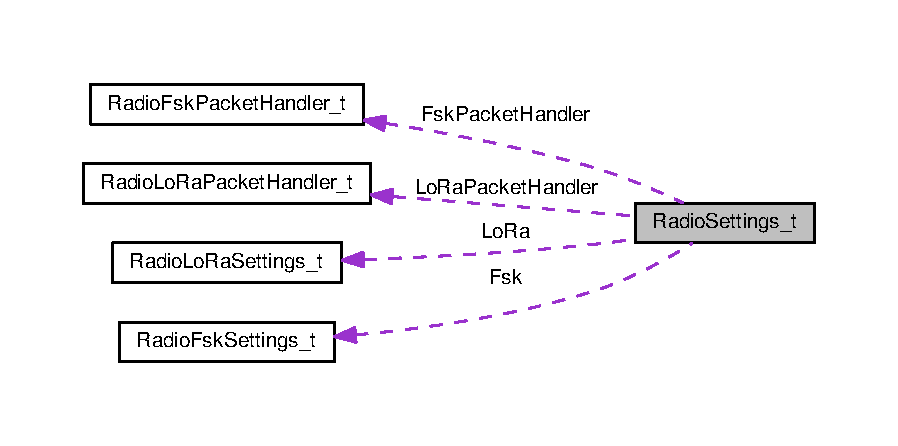
\includegraphics[width=350pt]{structRadioSettings__t__coll__graph}
\end{center}
\end{figure}
\subsection*{Data Fields}
\begin{DoxyCompactItemize}
\item 
Radio\+State\+\_\+t \hyperlink{structRadioSettings__t_ad051d6eb4b33aa5a5027e84535821d63}{State}
\item 
Radio\+Modems\+\_\+t \hyperlink{structRadioSettings__t_a30e9dbea56513318361cffc63da1e4dc}{Modem}
\item 
uint32\+\_\+t \hyperlink{structRadioSettings__t_a7dff792a3ddef7633de17b2e41b8d074}{Channel}
\item 
\hyperlink{structRadioFskSettings__t}{Radio\+Fsk\+Settings\+\_\+t} \hyperlink{structRadioSettings__t_adc7c8d98b4b44e6483234246d6b67556}{Fsk}
\item 
\hyperlink{structRadioFskPacketHandler__t}{Radio\+Fsk\+Packet\+Handler\+\_\+t} \hyperlink{structRadioSettings__t_a72eaff1f3b89014d493768dd3c00f2d2}{Fsk\+Packet\+Handler}
\item 
\hyperlink{structRadioLoRaSettings__t}{Radio\+Lo\+Ra\+Settings\+\_\+t} \hyperlink{structRadioSettings__t_a36e1e4227a9444c96c670eb4343b1a16}{Lo\+Ra}
\item 
\hyperlink{structRadioLoRaPacketHandler__t}{Radio\+Lo\+Ra\+Packet\+Handler\+\_\+t} \hyperlink{structRadioSettings__t_a1a94014a708421cec9ff3095e5614784}{Lo\+Ra\+Packet\+Handler}
\end{DoxyCompactItemize}


\subsection{Detailed Description}
Radio Settings 

\subsection{Field Documentation}
\mbox{\Hypertarget{structRadioSettings__t_a7dff792a3ddef7633de17b2e41b8d074}\label{structRadioSettings__t_a7dff792a3ddef7633de17b2e41b8d074}} 
\index{Radio\+Settings\+\_\+t@{Radio\+Settings\+\_\+t}!Channel@{Channel}}
\index{Channel@{Channel}!Radio\+Settings\+\_\+t@{Radio\+Settings\+\_\+t}}
\subsubsection{\texorpdfstring{Channel}{Channel}}
{\footnotesize\ttfamily uint32\+\_\+t Radio\+Settings\+\_\+t\+::\+Channel}

\mbox{\Hypertarget{structRadioSettings__t_adc7c8d98b4b44e6483234246d6b67556}\label{structRadioSettings__t_adc7c8d98b4b44e6483234246d6b67556}} 
\index{Radio\+Settings\+\_\+t@{Radio\+Settings\+\_\+t}!Fsk@{Fsk}}
\index{Fsk@{Fsk}!Radio\+Settings\+\_\+t@{Radio\+Settings\+\_\+t}}
\subsubsection{\texorpdfstring{Fsk}{Fsk}}
{\footnotesize\ttfamily \hyperlink{structRadioFskSettings__t}{Radio\+Fsk\+Settings\+\_\+t} Radio\+Settings\+\_\+t\+::\+Fsk}

\mbox{\Hypertarget{structRadioSettings__t_a72eaff1f3b89014d493768dd3c00f2d2}\label{structRadioSettings__t_a72eaff1f3b89014d493768dd3c00f2d2}} 
\index{Radio\+Settings\+\_\+t@{Radio\+Settings\+\_\+t}!Fsk\+Packet\+Handler@{Fsk\+Packet\+Handler}}
\index{Fsk\+Packet\+Handler@{Fsk\+Packet\+Handler}!Radio\+Settings\+\_\+t@{Radio\+Settings\+\_\+t}}
\subsubsection{\texorpdfstring{Fsk\+Packet\+Handler}{FskPacketHandler}}
{\footnotesize\ttfamily \hyperlink{structRadioFskPacketHandler__t}{Radio\+Fsk\+Packet\+Handler\+\_\+t} Radio\+Settings\+\_\+t\+::\+Fsk\+Packet\+Handler}

\mbox{\Hypertarget{structRadioSettings__t_a36e1e4227a9444c96c670eb4343b1a16}\label{structRadioSettings__t_a36e1e4227a9444c96c670eb4343b1a16}} 
\index{Radio\+Settings\+\_\+t@{Radio\+Settings\+\_\+t}!Lo\+Ra@{Lo\+Ra}}
\index{Lo\+Ra@{Lo\+Ra}!Radio\+Settings\+\_\+t@{Radio\+Settings\+\_\+t}}
\subsubsection{\texorpdfstring{Lo\+Ra}{LoRa}}
{\footnotesize\ttfamily \hyperlink{structRadioLoRaSettings__t}{Radio\+Lo\+Ra\+Settings\+\_\+t} Radio\+Settings\+\_\+t\+::\+Lo\+Ra}

\mbox{\Hypertarget{structRadioSettings__t_a1a94014a708421cec9ff3095e5614784}\label{structRadioSettings__t_a1a94014a708421cec9ff3095e5614784}} 
\index{Radio\+Settings\+\_\+t@{Radio\+Settings\+\_\+t}!Lo\+Ra\+Packet\+Handler@{Lo\+Ra\+Packet\+Handler}}
\index{Lo\+Ra\+Packet\+Handler@{Lo\+Ra\+Packet\+Handler}!Radio\+Settings\+\_\+t@{Radio\+Settings\+\_\+t}}
\subsubsection{\texorpdfstring{Lo\+Ra\+Packet\+Handler}{LoRaPacketHandler}}
{\footnotesize\ttfamily \hyperlink{structRadioLoRaPacketHandler__t}{Radio\+Lo\+Ra\+Packet\+Handler\+\_\+t} Radio\+Settings\+\_\+t\+::\+Lo\+Ra\+Packet\+Handler}

\mbox{\Hypertarget{structRadioSettings__t_a30e9dbea56513318361cffc63da1e4dc}\label{structRadioSettings__t_a30e9dbea56513318361cffc63da1e4dc}} 
\index{Radio\+Settings\+\_\+t@{Radio\+Settings\+\_\+t}!Modem@{Modem}}
\index{Modem@{Modem}!Radio\+Settings\+\_\+t@{Radio\+Settings\+\_\+t}}
\subsubsection{\texorpdfstring{Modem}{Modem}}
{\footnotesize\ttfamily Radio\+Modems\+\_\+t Radio\+Settings\+\_\+t\+::\+Modem}

\mbox{\Hypertarget{structRadioSettings__t_ad051d6eb4b33aa5a5027e84535821d63}\label{structRadioSettings__t_ad051d6eb4b33aa5a5027e84535821d63}} 
\index{Radio\+Settings\+\_\+t@{Radio\+Settings\+\_\+t}!State@{State}}
\index{State@{State}!Radio\+Settings\+\_\+t@{Radio\+Settings\+\_\+t}}
\subsubsection{\texorpdfstring{State}{State}}
{\footnotesize\ttfamily Radio\+State\+\_\+t Radio\+Settings\+\_\+t\+::\+State}



The documentation for this struct was generated from the following file\+:\begin{DoxyCompactItemize}
\item 
Components/sx1276/\hyperlink{sx1276_8h}{sx1276.\+h}\end{DoxyCompactItemize}

\hypertarget{structsBoardCallback}{}\section{s\+Board\+Callback Struct Reference}
\label{structsBoardCallback}\index{s\+Board\+Callback@{s\+Board\+Callback}}


{\ttfamily \#include $<$sx1276.\+h$>$}

\subsection*{Data Fields}
\begin{DoxyCompactItemize}
\item 
void($\ast$ \hyperlink{structsBoardCallback_ae6be070dbcbbcdb0f30d087e6152dd55}{S\+X1276\+Board\+Set\+XO} )(uint8\+\_\+t state)
\begin{DoxyCompactList}\small\item\em Set XO state on the board. \end{DoxyCompactList}\item 
uint32\+\_\+t($\ast$ \hyperlink{structsBoardCallback_a91e24be9e9f398614e25b89d05ee0aa3}{S\+X1276\+Board\+Get\+Wake\+Time} )(void)
\begin{DoxyCompactList}\small\item\em Get Board Wake Up time. \end{DoxyCompactList}\item 
void($\ast$ \hyperlink{structsBoardCallback_ac8a78c18252b452f5f4305be2abd1f2c}{S\+X1276\+Board\+Io\+Irq\+Init} )(\hyperlink{sx1276_8h_af462584f307238535daaea42f6ce791c}{Dio\+Irq\+Handler} $\ast$$\ast$irq\+Handlers)
\begin{DoxyCompactList}\small\item\em Initializes the radio I/\+Os Irq. \end{DoxyCompactList}\item 
void($\ast$ \hyperlink{structsBoardCallback_aec7b6d1c4de061f3d2f1bebe75c64c13}{S\+X1276\+Board\+Set\+Rf\+Tx\+Power} )(int8\+\_\+t power)
\begin{DoxyCompactList}\small\item\em Sets the radio output power. \end{DoxyCompactList}\item 
void($\ast$ \hyperlink{structsBoardCallback_a91d44db14871cfcf950cce928922ba17}{S\+X1276\+Board\+Set\+Ant\+Sw\+Low\+Power} )(bool status)
\begin{DoxyCompactList}\small\item\em Set the RF Switch I/\+Os pins in Low Power mode. \end{DoxyCompactList}\item 
void($\ast$ \hyperlink{structsBoardCallback_a9c50d59b5bffe4261b6e141d503ea74a}{S\+X1276\+Board\+Set\+Ant\+Sw} )(uint8\+\_\+t op\+Mode)
\begin{DoxyCompactList}\small\item\em Controls the antena switch if necessary. \end{DoxyCompactList}\end{DoxyCompactItemize}


\subsection{Field Documentation}
\mbox{\Hypertarget{structsBoardCallback_a91e24be9e9f398614e25b89d05ee0aa3}\label{structsBoardCallback_a91e24be9e9f398614e25b89d05ee0aa3}} 
\index{s\+Board\+Callback@{s\+Board\+Callback}!S\+X1276\+Board\+Get\+Wake\+Time@{S\+X1276\+Board\+Get\+Wake\+Time}}
\index{S\+X1276\+Board\+Get\+Wake\+Time@{S\+X1276\+Board\+Get\+Wake\+Time}!s\+Board\+Callback@{s\+Board\+Callback}}
\subsubsection{\texorpdfstring{S\+X1276\+Board\+Get\+Wake\+Time}{SX1276BoardGetWakeTime}}
{\footnotesize\ttfamily uint32\+\_\+t( $\ast$ s\+Board\+Callback\+::\+S\+X1276\+Board\+Get\+Wake\+Time) (void)}



Get Board Wake Up time. 

\mbox{\Hypertarget{structsBoardCallback_ac8a78c18252b452f5f4305be2abd1f2c}\label{structsBoardCallback_ac8a78c18252b452f5f4305be2abd1f2c}} 
\index{s\+Board\+Callback@{s\+Board\+Callback}!S\+X1276\+Board\+Io\+Irq\+Init@{S\+X1276\+Board\+Io\+Irq\+Init}}
\index{S\+X1276\+Board\+Io\+Irq\+Init@{S\+X1276\+Board\+Io\+Irq\+Init}!s\+Board\+Callback@{s\+Board\+Callback}}
\subsubsection{\texorpdfstring{S\+X1276\+Board\+Io\+Irq\+Init}{SX1276BoardIoIrqInit}}
{\footnotesize\ttfamily void( $\ast$ s\+Board\+Callback\+::\+S\+X1276\+Board\+Io\+Irq\+Init) (\hyperlink{sx1276_8h_af462584f307238535daaea42f6ce791c}{Dio\+Irq\+Handler} $\ast$$\ast$irq\+Handlers)}



Initializes the radio I/\+Os Irq. 

\mbox{\Hypertarget{structsBoardCallback_a9c50d59b5bffe4261b6e141d503ea74a}\label{structsBoardCallback_a9c50d59b5bffe4261b6e141d503ea74a}} 
\index{s\+Board\+Callback@{s\+Board\+Callback}!S\+X1276\+Board\+Set\+Ant\+Sw@{S\+X1276\+Board\+Set\+Ant\+Sw}}
\index{S\+X1276\+Board\+Set\+Ant\+Sw@{S\+X1276\+Board\+Set\+Ant\+Sw}!s\+Board\+Callback@{s\+Board\+Callback}}
\subsubsection{\texorpdfstring{S\+X1276\+Board\+Set\+Ant\+Sw}{SX1276BoardSetAntSw}}
{\footnotesize\ttfamily void( $\ast$ s\+Board\+Callback\+::\+S\+X1276\+Board\+Set\+Ant\+Sw) (uint8\+\_\+t op\+Mode)}



Controls the antena switch if necessary. 

\begin{DoxyRemark}{Remarks}
see errata note
\end{DoxyRemark}

\begin{DoxyParams}{Parameters}
{\em \mbox{[}\+I\+N\mbox{]}} & op\+Mode Current radio operating mode \\
\hline
\end{DoxyParams}
\mbox{\Hypertarget{structsBoardCallback_a91d44db14871cfcf950cce928922ba17}\label{structsBoardCallback_a91d44db14871cfcf950cce928922ba17}} 
\index{s\+Board\+Callback@{s\+Board\+Callback}!S\+X1276\+Board\+Set\+Ant\+Sw\+Low\+Power@{S\+X1276\+Board\+Set\+Ant\+Sw\+Low\+Power}}
\index{S\+X1276\+Board\+Set\+Ant\+Sw\+Low\+Power@{S\+X1276\+Board\+Set\+Ant\+Sw\+Low\+Power}!s\+Board\+Callback@{s\+Board\+Callback}}
\subsubsection{\texorpdfstring{S\+X1276\+Board\+Set\+Ant\+Sw\+Low\+Power}{SX1276BoardSetAntSwLowPower}}
{\footnotesize\ttfamily void( $\ast$ s\+Board\+Callback\+::\+S\+X1276\+Board\+Set\+Ant\+Sw\+Low\+Power) (bool status)}



Set the RF Switch I/\+Os pins in Low Power mode. 


\begin{DoxyParams}{Parameters}
{\em \mbox{[}\+I\+N\mbox{]}} & status enable or disable \\
\hline
\end{DoxyParams}
\mbox{\Hypertarget{structsBoardCallback_aec7b6d1c4de061f3d2f1bebe75c64c13}\label{structsBoardCallback_aec7b6d1c4de061f3d2f1bebe75c64c13}} 
\index{s\+Board\+Callback@{s\+Board\+Callback}!S\+X1276\+Board\+Set\+Rf\+Tx\+Power@{S\+X1276\+Board\+Set\+Rf\+Tx\+Power}}
\index{S\+X1276\+Board\+Set\+Rf\+Tx\+Power@{S\+X1276\+Board\+Set\+Rf\+Tx\+Power}!s\+Board\+Callback@{s\+Board\+Callback}}
\subsubsection{\texorpdfstring{S\+X1276\+Board\+Set\+Rf\+Tx\+Power}{SX1276BoardSetRfTxPower}}
{\footnotesize\ttfamily void( $\ast$ s\+Board\+Callback\+::\+S\+X1276\+Board\+Set\+Rf\+Tx\+Power) (int8\+\_\+t power)}



Sets the radio output power. 


\begin{DoxyParams}{Parameters}
{\em \mbox{[}\+I\+N\mbox{]}} & power Sets the RF output power \\
\hline
\end{DoxyParams}
\mbox{\Hypertarget{structsBoardCallback_ae6be070dbcbbcdb0f30d087e6152dd55}\label{structsBoardCallback_ae6be070dbcbbcdb0f30d087e6152dd55}} 
\index{s\+Board\+Callback@{s\+Board\+Callback}!S\+X1276\+Board\+Set\+XO@{S\+X1276\+Board\+Set\+XO}}
\index{S\+X1276\+Board\+Set\+XO@{S\+X1276\+Board\+Set\+XO}!s\+Board\+Callback@{s\+Board\+Callback}}
\subsubsection{\texorpdfstring{S\+X1276\+Board\+Set\+XO}{SX1276BoardSetXO}}
{\footnotesize\ttfamily void( $\ast$ s\+Board\+Callback\+::\+S\+X1276\+Board\+Set\+XO) (uint8\+\_\+t state)}



Set XO state on the board. 



The documentation for this struct was generated from the following file\+:\begin{DoxyCompactItemize}
\item 
Components/sx1276/\hyperlink{sx1276_8h}{sx1276.\+h}\end{DoxyCompactItemize}

\hypertarget{structSX1276__s}{}\section{S\+X1276\+\_\+s Struct Reference}
\label{structSX1276__s}\index{S\+X1276\+\_\+s@{S\+X1276\+\_\+s}}


{\ttfamily \#include $<$sx1276.\+h$>$}



Collaboration diagram for S\+X1276\+\_\+s\+:
\nopagebreak
\begin{figure}[H]
\begin{center}
\leavevmode
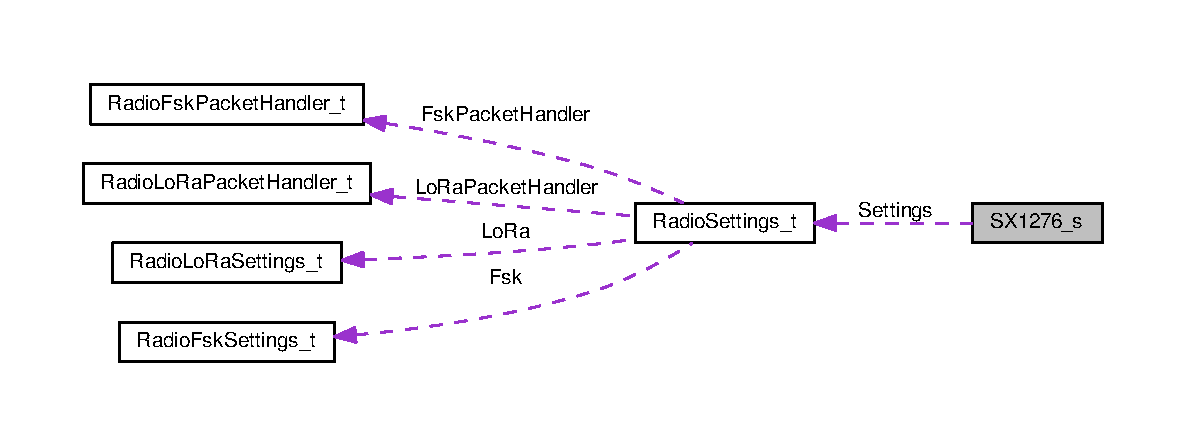
\includegraphics[width=350pt]{structSX1276__s__coll__graph}
\end{center}
\end{figure}
\subsection*{Data Fields}
\begin{DoxyCompactItemize}
\item 
uint8\+\_\+t \hyperlink{structSX1276__s_abef47b886ad9300944015058c8255411}{Rx\+Tx}
\item 
\hyperlink{structRadioSettings__t}{Radio\+Settings\+\_\+t} \hyperlink{structSX1276__s_aacf7afe5f1c4e05bc4822255dc8a123c}{Settings}
\end{DoxyCompactItemize}


\subsection{Detailed Description}
Radio hardware and global parameters 

\subsection{Field Documentation}
\mbox{\Hypertarget{structSX1276__s_abef47b886ad9300944015058c8255411}\label{structSX1276__s_abef47b886ad9300944015058c8255411}} 
\index{S\+X1276\+\_\+s@{S\+X1276\+\_\+s}!Rx\+Tx@{Rx\+Tx}}
\index{Rx\+Tx@{Rx\+Tx}!S\+X1276\+\_\+s@{S\+X1276\+\_\+s}}
\subsubsection{\texorpdfstring{Rx\+Tx}{RxTx}}
{\footnotesize\ttfamily uint8\+\_\+t S\+X1276\+\_\+s\+::\+Rx\+Tx}

\mbox{\Hypertarget{structSX1276__s_aacf7afe5f1c4e05bc4822255dc8a123c}\label{structSX1276__s_aacf7afe5f1c4e05bc4822255dc8a123c}} 
\index{S\+X1276\+\_\+s@{S\+X1276\+\_\+s}!Settings@{Settings}}
\index{Settings@{Settings}!S\+X1276\+\_\+s@{S\+X1276\+\_\+s}}
\subsubsection{\texorpdfstring{Settings}{Settings}}
{\footnotesize\ttfamily \hyperlink{structRadioSettings__t}{Radio\+Settings\+\_\+t} S\+X1276\+\_\+s\+::\+Settings}



The documentation for this struct was generated from the following file\+:\begin{DoxyCompactItemize}
\item 
Components/sx1276/\hyperlink{sx1276_8h}{sx1276.\+h}\end{DoxyCompactItemize}

\chapter{File Documentation}
\hypertarget{b-l072z-lrwan1_8c}{}\section{B-\/\+L072\+Z-\/\+L\+R\+W\+A\+N1/b-\/l072z-\/lrwan1.c File Reference}
\label{b-l072z-lrwan1_8c}\index{B-\/\+L072\+Z-\/\+L\+R\+W\+A\+N1/b-\/l072z-\/lrwan1.\+c@{B-\/\+L072\+Z-\/\+L\+R\+W\+A\+N1/b-\/l072z-\/lrwan1.\+c}}


This file contains definitions for\+:  


{\ttfamily \#include \char`\"{}b-\/l072z-\/lrwan1.\+h\char`\"{}}\newline
{\ttfamily \#include $<$stdlib.\+h$>$}\newline
Include dependency graph for b-\/l072z-\/lrwan1.c\+:
\nopagebreak
\begin{figure}[H]
\begin{center}
\leavevmode
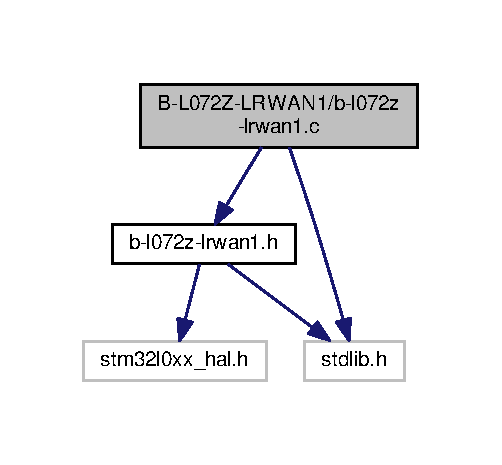
\includegraphics[width=241pt]{b-l072z-lrwan1_8c__incl}
\end{center}
\end{figure}
\subsection*{Macros}
\begin{DoxyCompactItemize}
\item 
\#define \hyperlink{group__B-L072Z-LRWAN1__LOW__LEVEL__Private__Defines_gaf5f53a499afef1aaa3850de7086a11a5}{\+\_\+\+\_\+\+B\+\_\+\+L072\+Z\+\_\+\+L\+R\+W\+A\+N1\+\_\+\+B\+S\+P\+\_\+\+V\+E\+R\+S\+I\+O\+N\+\_\+\+M\+A\+IN}~(0x01)
\begin{DoxyCompactList}\small\item\em 32\+L082\+M\+LM D\+I\+S\+CO B\+SP Driver version number V1.\+0.\+0 \end{DoxyCompactList}\item 
\#define \hyperlink{group__B-L072Z-LRWAN1__LOW__LEVEL__Private__Defines_ga682147e46afbdf8d1002615e3ff7ad4a}{\+\_\+\+\_\+\+B\+\_\+\+L072\+Z\+\_\+\+L\+R\+W\+A\+N1\+\_\+\+B\+S\+P\+\_\+\+V\+E\+R\+S\+I\+O\+N\+\_\+\+S\+U\+B1}~(0x00)
\item 
\#define \hyperlink{group__B-L072Z-LRWAN1__LOW__LEVEL__Private__Defines_gaf0b4c3a1aa8fd40d74fc5fe1c845059e}{\+\_\+\+\_\+\+B\+\_\+\+L072\+Z\+\_\+\+L\+R\+W\+A\+N1\+\_\+\+B\+S\+P\+\_\+\+V\+E\+R\+S\+I\+O\+N\+\_\+\+S\+U\+B2}~(0x00)
\item 
\#define \hyperlink{group__B-L072Z-LRWAN1__LOW__LEVEL__Private__Defines_ga1c5543dd393ec382e3cee4c35b86c9cd}{\+\_\+\+\_\+\+B\+\_\+\+L072\+Z\+\_\+\+L\+R\+W\+A\+N1\+\_\+\+B\+S\+P\+\_\+\+V\+E\+R\+S\+I\+O\+N\+\_\+\+RC}~(0x00)
\item 
\#define \hyperlink{group__B-L072Z-LRWAN1__LOW__LEVEL__Private__Defines_ga62f40f0f53b1c1d1f0aaaa7fb0b63d5f}{\+\_\+\+\_\+\+B\+\_\+\+L072\+Z\+\_\+\+L\+R\+W\+A\+N1\+\_\+\+B\+S\+P\+\_\+\+V\+E\+R\+S\+I\+ON}
\end{DoxyCompactItemize}
\subsection*{Functions}
\begin{DoxyCompactItemize}
\item 
uint32\+\_\+t \hyperlink{group__B-L072Z-LRWAN1__LOW__LEVEL__Private__Defines_ga65d13608f7010a8068614154cb142cd6}{B\+S\+P\+\_\+\+Get\+Version} (void)
\begin{DoxyCompactList}\small\item\em This method returns the B-\/\+L072\+Z-\/\+L\+R\+W\+A\+N1 B\+SP Driver revision. \end{DoxyCompactList}\item 
void \hyperlink{group__B-L072Z-LRWAN1__LOW__LEVEL__Private__Defines_gab58a4f16a476a53653c5c400e3bed158}{B\+S\+P\+\_\+\+L\+E\+D\+\_\+\+Init} (\hyperlink{group__B-L072Z-LRWAN1__LOW__LEVEL__Exported__Types_gaa059704b7ca945eb9c1e7f2c3d03fecd}{Led\+\_\+\+Type\+Def} Led)
\begin{DoxyCompactList}\small\item\em Configures L\+ED G\+P\+IO. \end{DoxyCompactList}\item 
void \hyperlink{group__B-L072Z-LRWAN1__LOW__LEVEL__Private__Defines_gaee9c16b16384834c69efabf58f423d6f}{B\+S\+P\+\_\+\+L\+E\+D\+\_\+\+On} (\hyperlink{group__B-L072Z-LRWAN1__LOW__LEVEL__Exported__Types_gaa059704b7ca945eb9c1e7f2c3d03fecd}{Led\+\_\+\+Type\+Def} Led)
\begin{DoxyCompactList}\small\item\em Turns selected L\+ED On. \end{DoxyCompactList}\item 
void \hyperlink{group__B-L072Z-LRWAN1__LOW__LEVEL__Private__Defines_gaef268680154ca15c45066d64d41f9467}{B\+S\+P\+\_\+\+L\+E\+D\+\_\+\+Off} (\hyperlink{group__B-L072Z-LRWAN1__LOW__LEVEL__Exported__Types_gaa059704b7ca945eb9c1e7f2c3d03fecd}{Led\+\_\+\+Type\+Def} Led)
\begin{DoxyCompactList}\small\item\em Turns selected L\+ED Off. \end{DoxyCompactList}\item 
void \hyperlink{group__B-L072Z-LRWAN1__LOW__LEVEL__Private__Defines_ga1b9eabba7d498f41d6f16587ec0f9732}{B\+S\+P\+\_\+\+L\+E\+D\+\_\+\+Toggle} (\hyperlink{group__B-L072Z-LRWAN1__LOW__LEVEL__Exported__Types_gaa059704b7ca945eb9c1e7f2c3d03fecd}{Led\+\_\+\+Type\+Def} Led)
\begin{DoxyCompactList}\small\item\em Toggles the selected L\+ED. \end{DoxyCompactList}\item 
void \hyperlink{group__B-L072Z-LRWAN1__LOW__LEVEL__Private__Defines_gad31c8db50a71c1f6dbfe132d72ba0bc6}{B\+S\+P\+\_\+\+P\+B\+\_\+\+Init} (\hyperlink{group__B-L072Z-LRWAN1__LOW__LEVEL__Exported__Types_ga643816dfbad5c734fc25a29ce8d35bb1}{Button\+\_\+\+Type\+Def} Button, \hyperlink{group__B-L072Z-LRWAN1__LOW__LEVEL__Exported__Types_ga48825b7c7d851c440ef8e808fd9d8f0a}{Button\+Mode\+\_\+\+Type\+Def} Button\+Mode)
\begin{DoxyCompactList}\small\item\em Configures Button G\+P\+IO and E\+X\+TI Line. \end{DoxyCompactList}\item 
uint32\+\_\+t \hyperlink{group__B-L072Z-LRWAN1__LOW__LEVEL__Private__Defines_ga8f0978b6cffda9c67266ddfdb3a0abf7}{B\+S\+P\+\_\+\+P\+B\+\_\+\+Get\+State} (\hyperlink{group__B-L072Z-LRWAN1__LOW__LEVEL__Exported__Types_ga643816dfbad5c734fc25a29ce8d35bb1}{Button\+\_\+\+Type\+Def} Button)
\begin{DoxyCompactList}\small\item\em Returns the selected Button state. \end{DoxyCompactList}\end{DoxyCompactItemize}
\subsection*{Variables}
\begin{DoxyCompactItemize}
\item 
G\+P\+I\+O\+\_\+\+Type\+Def $\ast$ \hyperlink{group__B-L072Z-LRWAN1__LOW__LEVEL__Private__Variables_ga1127c0cf12e4ec7a66f2a64cd7407218}{L\+E\+D\+\_\+\+P\+O\+RT} \mbox{[}\hyperlink{group__B-L072Z-LRWAN1__LOW__LEVEL__LED_gab4be2480bf7d44d52aab1190a65a733c}{L\+E\+Dn}\mbox{]} = \{\hyperlink{group__B-L072Z-LRWAN1__LOW__LEVEL__LED_ga5d97443b4011e40e47164445dc1adde0}{L\+E\+D1\+\_\+\+G\+P\+I\+O\+\_\+\+P\+O\+RT}, \hyperlink{group__B-L072Z-LRWAN1__LOW__LEVEL__LED_gaf88822ae4b79d37c7735ce1160b59f68}{L\+E\+D2\+\_\+\+G\+P\+I\+O\+\_\+\+P\+O\+RT}, \hyperlink{group__B-L072Z-LRWAN1__LOW__LEVEL__LED_ga050f4b3a1f402476f9541dfe975d2143}{L\+E\+D3\+\_\+\+G\+P\+I\+O\+\_\+\+P\+O\+RT}, \hyperlink{group__B-L072Z-LRWAN1__LOW__LEVEL__LED_ga6b6f3eb4d23b770de265803afbc2b61b}{L\+E\+D4\+\_\+\+G\+P\+I\+O\+\_\+\+P\+O\+RT}\}
\item 
const uint16\+\_\+t \hyperlink{group__B-L072Z-LRWAN1__LOW__LEVEL__Private__Variables_ga51722a2d3aff3970f123a94ac62b908f}{L\+E\+D\+\_\+\+P\+IN} \mbox{[}\hyperlink{group__B-L072Z-LRWAN1__LOW__LEVEL__LED_gab4be2480bf7d44d52aab1190a65a733c}{L\+E\+Dn}\mbox{]} = \{\hyperlink{group__B-L072Z-LRWAN1__LOW__LEVEL__LED_ga318aa17e5d40e2132d2c7f6269ce7f51}{L\+E\+D1\+\_\+\+P\+IN}, \hyperlink{group__B-L072Z-LRWAN1__LOW__LEVEL__LED_gaf6f84078113b55354d20585131b386f7}{L\+E\+D2\+\_\+\+P\+IN},\hyperlink{group__B-L072Z-LRWAN1__LOW__LEVEL__LED_ga4cb3ff938bcabb01494ce529ae55a542}{L\+E\+D3\+\_\+\+P\+IN}, \hyperlink{group__B-L072Z-LRWAN1__LOW__LEVEL__LED_gaae684bb3d2f940637ccbc2adeb0e134d}{L\+E\+D4\+\_\+\+P\+IN}\}
\item 
G\+P\+I\+O\+\_\+\+Type\+Def $\ast$ \hyperlink{group__B-L072Z-LRWAN1__LOW__LEVEL__Private__Variables_gad63ed42b4071e78f80f7462227da4f35}{B\+U\+T\+T\+O\+N\+\_\+\+P\+O\+RT} \mbox{[}\hyperlink{group__B-L072Z-LRWAN1__LOW__LEVEL__BUTTON_ga43d47e509ada64329393005c3be15d64}{B\+U\+T\+T\+O\+Nn}\mbox{]} = \{\hyperlink{group__B-L072Z-LRWAN1__LOW__LEVEL__BUTTON_ga98680733a6992dacef531bfd0c23031c}{K\+E\+Y\+\_\+\+B\+U\+T\+T\+O\+N\+\_\+\+G\+P\+I\+O\+\_\+\+P\+O\+RT} \}
\item 
const uint16\+\_\+t \hyperlink{group__B-L072Z-LRWAN1__LOW__LEVEL__Private__Variables_gadf78f2d71408a01f8d30929c2d2da82b}{B\+U\+T\+T\+O\+N\+\_\+\+P\+IN} \mbox{[}\hyperlink{group__B-L072Z-LRWAN1__LOW__LEVEL__BUTTON_ga43d47e509ada64329393005c3be15d64}{B\+U\+T\+T\+O\+Nn}\mbox{]} = \{\hyperlink{group__B-L072Z-LRWAN1__LOW__LEVEL__BUTTON_ga5c260a4b4e26836dc3a9b6f15d317421}{K\+E\+Y\+\_\+\+B\+U\+T\+T\+O\+N\+\_\+\+P\+IN} \}
\item 
const uint8\+\_\+t \hyperlink{group__B-L072Z-LRWAN1__LOW__LEVEL__Private__Variables_ga13c3e27c584df9fccc4697dd535ea1cd}{B\+U\+T\+T\+O\+N\+\_\+\+I\+R\+Qn} \mbox{[}\hyperlink{group__B-L072Z-LRWAN1__LOW__LEVEL__BUTTON_ga43d47e509ada64329393005c3be15d64}{B\+U\+T\+T\+O\+Nn}\mbox{]} = \{\hyperlink{group__B-L072Z-LRWAN1__LOW__LEVEL__BUTTON_gaeb5bffe8281b0754675cfdfb2847e82d}{K\+E\+Y\+\_\+\+B\+U\+T\+T\+O\+N\+\_\+\+E\+X\+T\+I\+\_\+\+I\+R\+Qn} \}
\end{DoxyCompactItemize}


\subsection{Detailed Description}
This file contains definitions for\+: 

\begin{DoxyAuthor}{Author}
M\+CD Application Team 
\end{DoxyAuthor}
\begin{DoxyVersion}{Version}
V1.\+0.\+0 
\end{DoxyVersion}
\begin{DoxyDate}{Date}
15-\/\+November-\/2016
\begin{DoxyItemize}
\item L\+E\+Ds and push-\/button available on B-\/\+L072\+Z-\/\+L\+R\+W\+A\+N1 Discovery Kit from S\+T\+Microelectronics
\end{DoxyItemize}
\end{DoxyDate}
\begin{DoxyAttention}{Attention}

\end{DoxyAttention}
\subsubsection*{\begin{center}\copyright{} C\+O\+P\+Y\+R\+I\+G\+H\+T(c) 2015 S\+T\+Microelectronics\end{center} }

Redistribution and use in source and binary forms, with or without modification, are permitted provided that the following conditions are met\+:
\begin{DoxyEnumerate}
\item Redistributions of source code must retain the above copyright notice, this list of conditions and the following disclaimer.
\item Redistributions in binary form must reproduce the above copyright notice, this list of conditions and the following disclaimer in the documentation and/or other materials provided with the distribution.
\item Neither the name of S\+T\+Microelectronics nor the names of its contributors may be used to endorse or promote products derived from this software without specific prior written permission.
\end{DoxyEnumerate}

T\+H\+IS S\+O\+F\+T\+W\+A\+RE IS P\+R\+O\+V\+I\+D\+ED BY T\+HE C\+O\+P\+Y\+R\+I\+G\+HT H\+O\+L\+D\+E\+RS A\+ND C\+O\+N\+T\+R\+I\+B\+U\+T\+O\+RS \char`\"{}\+A\+S I\+S\char`\"{} A\+ND A\+NY E\+X\+P\+R\+E\+SS OR I\+M\+P\+L\+I\+ED W\+A\+R\+R\+A\+N\+T\+I\+ES, I\+N\+C\+L\+U\+D\+I\+NG, B\+UT N\+OT L\+I\+M\+I\+T\+ED TO, T\+HE I\+M\+P\+L\+I\+ED W\+A\+R\+R\+A\+N\+T\+I\+ES OF M\+E\+R\+C\+H\+A\+N\+T\+A\+B\+I\+L\+I\+TY A\+ND F\+I\+T\+N\+E\+SS F\+OR A P\+A\+R\+T\+I\+C\+U\+L\+AR P\+U\+R\+P\+O\+SE A\+RE D\+I\+S\+C\+L\+A\+I\+M\+ED. IN NO E\+V\+E\+NT S\+H\+A\+LL T\+HE C\+O\+P\+Y\+R\+I\+G\+HT H\+O\+L\+D\+ER OR C\+O\+N\+T\+R\+I\+B\+U\+T\+O\+RS BE L\+I\+A\+B\+LE F\+OR A\+NY D\+I\+R\+E\+CT, I\+N\+D\+I\+R\+E\+CT, I\+N\+C\+I\+D\+E\+N\+T\+AL, S\+P\+E\+C\+I\+AL, E\+X\+E\+M\+P\+L\+A\+RY, OR C\+O\+N\+S\+E\+Q\+U\+E\+N\+T\+I\+AL D\+A\+M\+A\+G\+ES (I\+N\+C\+L\+U\+D\+I\+NG, B\+UT N\+OT L\+I\+M\+I\+T\+ED TO, P\+R\+O\+C\+U\+R\+E\+M\+E\+NT OF S\+U\+B\+S\+T\+I\+T\+U\+TE G\+O\+O\+DS OR S\+E\+R\+V\+I\+C\+ES; L\+O\+SS OF U\+SE, D\+A\+TA, OR P\+R\+O\+F\+I\+TS; OR B\+U\+S\+I\+N\+E\+SS I\+N\+T\+E\+R\+R\+U\+P\+T\+I\+ON) H\+O\+W\+E\+V\+ER C\+A\+U\+S\+ED A\+ND ON A\+NY T\+H\+E\+O\+RY OF L\+I\+A\+B\+I\+L\+I\+TY, W\+H\+E\+T\+H\+ER IN C\+O\+N\+T\+R\+A\+CT, S\+T\+R\+I\+CT L\+I\+A\+B\+I\+L\+I\+TY, OR T\+O\+RT (I\+N\+C\+L\+U\+D\+I\+NG N\+E\+G\+L\+I\+G\+E\+N\+CE OR O\+T\+H\+E\+R\+W\+I\+SE) A\+R\+I\+S\+I\+NG IN A\+NY W\+AY O\+UT OF T\+HE U\+SE OF T\+H\+IS S\+O\+F\+T\+W\+A\+RE, E\+V\+EN IF A\+D\+V\+I\+S\+ED OF T\+HE P\+O\+S\+S\+I\+B\+I\+L\+I\+TY OF S\+U\+CH D\+A\+M\+A\+GE. 
\hypertarget{b-l072z-lrwan1_8h}{}\section{B-\/\+L072\+Z-\/\+L\+R\+W\+A\+N1/b-\/l072z-\/lrwan1.h File Reference}
\label{b-l072z-lrwan1_8h}\index{B-\/\+L072\+Z-\/\+L\+R\+W\+A\+N1/b-\/l072z-\/lrwan1.\+h@{B-\/\+L072\+Z-\/\+L\+R\+W\+A\+N1/b-\/l072z-\/lrwan1.\+h}}


This file contains definitions for\+:  


{\ttfamily \#include \char`\"{}stm32l0xx\+\_\+hal.\+h\char`\"{}}\newline
{\ttfamily \#include \char`\"{}stdlib.\+h\char`\"{}}\newline
Include dependency graph for b-\/l072z-\/lrwan1.h\+:
\nopagebreak
\begin{figure}[H]
\begin{center}
\leavevmode
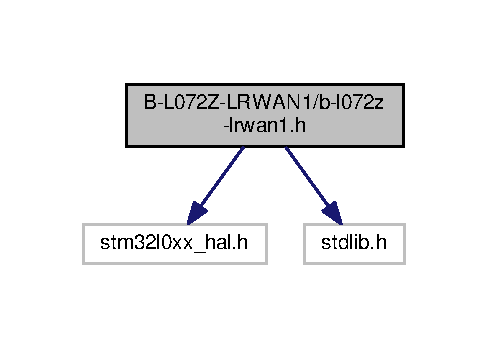
\includegraphics[width=234pt]{b-l072z-lrwan1_8h__incl}
\end{center}
\end{figure}
This graph shows which files directly or indirectly include this file\+:
\nopagebreak
\begin{figure}[H]
\begin{center}
\leavevmode
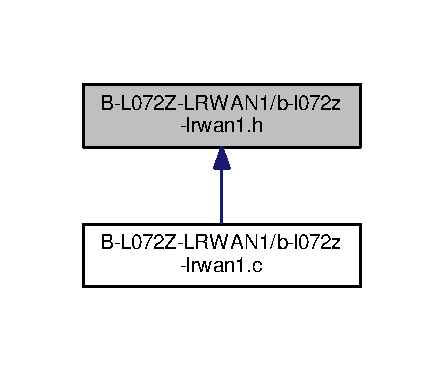
\includegraphics[width=213pt]{b-l072z-lrwan1_8h__dep__incl}
\end{center}
\end{figure}
\subsection*{Macros}
\begin{DoxyCompactItemize}
\item 
\#define \hyperlink{group__B-L072Z-LRWAN1__LOW__LEVEL__LED_gab4be2480bf7d44d52aab1190a65a733c}{L\+E\+Dn}~4
\item 
\#define \hyperlink{group__B-L072Z-LRWAN1__LOW__LEVEL__LED_ga318aa17e5d40e2132d2c7f6269ce7f51}{L\+E\+D1\+\_\+\+P\+IN}~G\+P\+I\+O\+\_\+\+P\+I\+N\+\_\+5
\item 
\#define \hyperlink{group__B-L072Z-LRWAN1__LOW__LEVEL__LED_ga5d97443b4011e40e47164445dc1adde0}{L\+E\+D1\+\_\+\+G\+P\+I\+O\+\_\+\+P\+O\+RT}~G\+P\+I\+OB
\item 
\#define \hyperlink{group__B-L072Z-LRWAN1__LOW__LEVEL__LED_gae90d969ab305110513ff3c2c0874f2e7}{L\+E\+D1\+\_\+\+G\+P\+I\+O\+\_\+\+C\+L\+K\+\_\+\+E\+N\+A\+B\+LE}()~\+\_\+\+\_\+\+H\+A\+L\+\_\+\+R\+C\+C\+\_\+\+G\+P\+I\+O\+B\+\_\+\+C\+L\+K\+\_\+\+E\+N\+A\+B\+LE()
\item 
\#define \hyperlink{group__B-L072Z-LRWAN1__LOW__LEVEL__LED_ga62e716eb8db20c4eccd17c29968d67c4}{L\+E\+D1\+\_\+\+G\+P\+I\+O\+\_\+\+C\+L\+K\+\_\+\+D\+I\+S\+A\+B\+LE}()~\+\_\+\+\_\+\+H\+A\+L\+\_\+\+R\+C\+C\+\_\+\+G\+P\+I\+O\+B\+\_\+\+C\+L\+K\+\_\+\+D\+I\+S\+A\+B\+LE()
\item 
\#define \hyperlink{group__B-L072Z-LRWAN1__LOW__LEVEL__LED_gaf6f84078113b55354d20585131b386f7}{L\+E\+D2\+\_\+\+P\+IN}~G\+P\+I\+O\+\_\+\+P\+I\+N\+\_\+5
\item 
\#define \hyperlink{group__B-L072Z-LRWAN1__LOW__LEVEL__LED_gaf88822ae4b79d37c7735ce1160b59f68}{L\+E\+D2\+\_\+\+G\+P\+I\+O\+\_\+\+P\+O\+RT}~G\+P\+I\+OA
\item 
\#define \hyperlink{group__B-L072Z-LRWAN1__LOW__LEVEL__LED_ga810e6c23b9a3e66da601b0058ec7a245}{L\+E\+D2\+\_\+\+G\+P\+I\+O\+\_\+\+C\+L\+K\+\_\+\+E\+N\+A\+B\+LE}()~\+\_\+\+\_\+\+H\+A\+L\+\_\+\+R\+C\+C\+\_\+\+G\+P\+I\+O\+A\+\_\+\+C\+L\+K\+\_\+\+E\+N\+A\+B\+LE()
\item 
\#define \hyperlink{group__B-L072Z-LRWAN1__LOW__LEVEL__LED_ga57f4d9343f3fe6d94d83ab2cb45c7d75}{L\+E\+D2\+\_\+\+G\+P\+I\+O\+\_\+\+C\+L\+K\+\_\+\+D\+I\+S\+A\+B\+LE}()~\+\_\+\+\_\+\+H\+A\+L\+\_\+\+R\+C\+C\+\_\+\+G\+P\+I\+O\+A\+\_\+\+C\+L\+K\+\_\+\+D\+I\+S\+A\+B\+LE()
\item 
\#define \hyperlink{group__B-L072Z-LRWAN1__LOW__LEVEL__LED_ga4cb3ff938bcabb01494ce529ae55a542}{L\+E\+D3\+\_\+\+P\+IN}~G\+P\+I\+O\+\_\+\+P\+I\+N\+\_\+6
\item 
\#define \hyperlink{group__B-L072Z-LRWAN1__LOW__LEVEL__LED_ga050f4b3a1f402476f9541dfe975d2143}{L\+E\+D3\+\_\+\+G\+P\+I\+O\+\_\+\+P\+O\+RT}~G\+P\+I\+OB
\item 
\#define \hyperlink{group__B-L072Z-LRWAN1__LOW__LEVEL__LED_gaac6c1162fc6bf1b60265e6fb7622e306}{L\+E\+D3\+\_\+\+G\+P\+I\+O\+\_\+\+C\+L\+K\+\_\+\+E\+N\+A\+B\+LE}()~\+\_\+\+\_\+\+H\+A\+L\+\_\+\+R\+C\+C\+\_\+\+G\+P\+I\+O\+B\+\_\+\+C\+L\+K\+\_\+\+E\+N\+A\+B\+LE()
\item 
\#define \hyperlink{group__B-L072Z-LRWAN1__LOW__LEVEL__LED_ga705278d726c1340f18576ca2d74f6e81}{L\+E\+D3\+\_\+\+G\+P\+I\+O\+\_\+\+C\+L\+K\+\_\+\+D\+I\+S\+A\+B\+LE}()~\+\_\+\+\_\+\+H\+A\+L\+\_\+\+R\+C\+C\+\_\+\+G\+P\+I\+O\+B\+\_\+\+C\+L\+K\+\_\+\+D\+I\+S\+A\+B\+LE()
\item 
\#define \hyperlink{group__B-L072Z-LRWAN1__LOW__LEVEL__LED_gaae684bb3d2f940637ccbc2adeb0e134d}{L\+E\+D4\+\_\+\+P\+IN}~G\+P\+I\+O\+\_\+\+P\+I\+N\+\_\+7
\item 
\#define \hyperlink{group__B-L072Z-LRWAN1__LOW__LEVEL__LED_ga6b6f3eb4d23b770de265803afbc2b61b}{L\+E\+D4\+\_\+\+G\+P\+I\+O\+\_\+\+P\+O\+RT}~G\+P\+I\+OB
\item 
\#define \hyperlink{group__B-L072Z-LRWAN1__LOW__LEVEL__LED_ga301aa5a187b24af8c121a462d2b08deb}{L\+E\+D4\+\_\+\+G\+P\+I\+O\+\_\+\+C\+L\+K\+\_\+\+E\+N\+A\+B\+LE}()~\+\_\+\+\_\+\+H\+A\+L\+\_\+\+R\+C\+C\+\_\+\+G\+P\+I\+O\+B\+\_\+\+C\+L\+K\+\_\+\+E\+N\+A\+B\+LE()
\item 
\#define \hyperlink{group__B-L072Z-LRWAN1__LOW__LEVEL__LED_ga9c737fb47feaa0f730edbe5251750353}{L\+E\+D4\+\_\+\+G\+P\+I\+O\+\_\+\+C\+L\+K\+\_\+\+D\+I\+S\+A\+B\+LE}()~\+\_\+\+\_\+\+H\+A\+L\+\_\+\+R\+C\+C\+\_\+\+G\+P\+I\+O\+B\+\_\+\+C\+L\+K\+\_\+\+D\+I\+S\+A\+B\+LE()
\item 
\#define \hyperlink{group__B-L072Z-LRWAN1__LOW__LEVEL__LED_ga32faaf3f04d44e7eddce1d781587fc57}{L\+E\+Dx\+\_\+\+G\+P\+I\+O\+\_\+\+C\+L\+K\+\_\+\+E\+N\+A\+B\+LE}(\+\_\+\+\_\+\+I\+N\+D\+E\+X\+\_\+\+\_\+)
\item 
\#define \hyperlink{group__B-L072Z-LRWAN1__LOW__LEVEL__LED_gaced1ef8f2a770d8c516ebc499b291df1}{L\+E\+Dx\+\_\+\+G\+P\+I\+O\+\_\+\+C\+L\+K\+\_\+\+D\+I\+S\+A\+B\+LE}(\+\_\+\+\_\+\+I\+N\+D\+E\+X\+\_\+\+\_\+)
\item 
\#define \hyperlink{group__B-L072Z-LRWAN1__LOW__LEVEL__BUTTON_ga43d47e509ada64329393005c3be15d64}{B\+U\+T\+T\+O\+Nn}~1
\item 
\#define \hyperlink{group__B-L072Z-LRWAN1__LOW__LEVEL__BUTTON_ga34df6915e3013d6a0c74131d3946b659}{U\+S\+E\+R\+\_\+\+B\+U\+T\+T\+O\+N\+\_\+\+P\+IN}~G\+P\+I\+O\+\_\+\+P\+I\+N\+\_\+2
\begin{DoxyCompactList}\small\item\em Key push-\/button. \end{DoxyCompactList}\item 
\#define \hyperlink{group__B-L072Z-LRWAN1__LOW__LEVEL__BUTTON_gae2e6fc2fdfda22b4eed3667375a8bd81}{U\+S\+E\+R\+\_\+\+B\+U\+T\+T\+O\+N\+\_\+\+G\+P\+I\+O\+\_\+\+P\+O\+RT}~G\+P\+I\+OB
\item 
\#define \hyperlink{group__B-L072Z-LRWAN1__LOW__LEVEL__BUTTON_gaa1f35ca26b42710d057661b54ace7d82}{U\+S\+E\+R\+\_\+\+B\+U\+T\+T\+O\+N\+\_\+\+G\+P\+I\+O\+\_\+\+C\+L\+K\+\_\+\+E\+N\+A\+B\+LE}()~\+\_\+\+\_\+\+H\+A\+L\+\_\+\+R\+C\+C\+\_\+\+G\+P\+I\+O\+B\+\_\+\+C\+L\+K\+\_\+\+E\+N\+A\+B\+LE()
\item 
\#define \hyperlink{group__B-L072Z-LRWAN1__LOW__LEVEL__BUTTON_ga71af1d1eec8f8b424b72f625abaad282}{U\+S\+E\+R\+\_\+\+B\+U\+T\+T\+O\+N\+\_\+\+G\+P\+I\+O\+\_\+\+C\+L\+K\+\_\+\+D\+I\+S\+A\+B\+LE}()~\+\_\+\+\_\+\+H\+A\+L\+\_\+\+R\+C\+C\+\_\+\+G\+P\+I\+O\+B\+\_\+\+C\+L\+K\+\_\+\+D\+I\+S\+A\+B\+LE()
\item 
\#define \hyperlink{group__B-L072Z-LRWAN1__LOW__LEVEL__BUTTON_gac41d04c2244ba780e4749991c85d1e9a}{U\+S\+E\+R\+\_\+\+B\+U\+T\+T\+O\+N\+\_\+\+E\+X\+T\+I\+\_\+\+L\+I\+NE}~G\+P\+I\+O\+\_\+\+P\+I\+N\+\_\+2
\item 
\#define \hyperlink{group__B-L072Z-LRWAN1__LOW__LEVEL__BUTTON_ga2e6e65a053529869d1c370610825d98f}{U\+S\+E\+R\+\_\+\+B\+U\+T\+T\+O\+N\+\_\+\+E\+X\+T\+I\+\_\+\+I\+R\+Qn}~E\+X\+T\+I2\+\_\+3\+\_\+\+I\+R\+Qn
\item 
\#define \hyperlink{group__B-L072Z-LRWAN1__LOW__LEVEL__BUTTON_ga5c260a4b4e26836dc3a9b6f15d317421}{K\+E\+Y\+\_\+\+B\+U\+T\+T\+O\+N\+\_\+\+P\+IN}~\hyperlink{group__B-L072Z-LRWAN1__LOW__LEVEL__BUTTON_ga34df6915e3013d6a0c74131d3946b659}{U\+S\+E\+R\+\_\+\+B\+U\+T\+T\+O\+N\+\_\+\+P\+IN}
\item 
\#define \hyperlink{group__B-L072Z-LRWAN1__LOW__LEVEL__BUTTON_ga98680733a6992dacef531bfd0c23031c}{K\+E\+Y\+\_\+\+B\+U\+T\+T\+O\+N\+\_\+\+G\+P\+I\+O\+\_\+\+P\+O\+RT}~\hyperlink{group__B-L072Z-LRWAN1__LOW__LEVEL__BUTTON_gae2e6fc2fdfda22b4eed3667375a8bd81}{U\+S\+E\+R\+\_\+\+B\+U\+T\+T\+O\+N\+\_\+\+G\+P\+I\+O\+\_\+\+P\+O\+RT}
\item 
\#define \hyperlink{group__B-L072Z-LRWAN1__LOW__LEVEL__BUTTON_ga6237d656da42b750f63cbf3e329096d5}{K\+E\+Y\+\_\+\+B\+U\+T\+T\+O\+N\+\_\+\+G\+P\+I\+O\+\_\+\+C\+L\+K\+\_\+\+E\+N\+A\+B\+LE}()~\hyperlink{group__B-L072Z-LRWAN1__LOW__LEVEL__BUTTON_gaa1f35ca26b42710d057661b54ace7d82}{U\+S\+E\+R\+\_\+\+B\+U\+T\+T\+O\+N\+\_\+\+G\+P\+I\+O\+\_\+\+C\+L\+K\+\_\+\+E\+N\+A\+B\+LE}()
\item 
\#define \hyperlink{group__B-L072Z-LRWAN1__LOW__LEVEL__BUTTON_gacf1a6a3b79ec610401d7ffbc1b6115d4}{K\+E\+Y\+\_\+\+B\+U\+T\+T\+O\+N\+\_\+\+G\+P\+I\+O\+\_\+\+C\+L\+K\+\_\+\+D\+I\+S\+A\+B\+LE}()~\hyperlink{group__B-L072Z-LRWAN1__LOW__LEVEL__BUTTON_ga71af1d1eec8f8b424b72f625abaad282}{U\+S\+E\+R\+\_\+\+B\+U\+T\+T\+O\+N\+\_\+\+G\+P\+I\+O\+\_\+\+C\+L\+K\+\_\+\+D\+I\+S\+A\+B\+LE}()
\item 
\#define \hyperlink{group__B-L072Z-LRWAN1__LOW__LEVEL__BUTTON_gae22d60d9f89ae7203bcd5ca8146bcef0}{K\+E\+Y\+\_\+\+B\+U\+T\+T\+O\+N\+\_\+\+E\+X\+T\+I\+\_\+\+L\+I\+NE}~\hyperlink{group__B-L072Z-LRWAN1__LOW__LEVEL__BUTTON_gac41d04c2244ba780e4749991c85d1e9a}{U\+S\+E\+R\+\_\+\+B\+U\+T\+T\+O\+N\+\_\+\+E\+X\+T\+I\+\_\+\+L\+I\+NE}
\item 
\#define \hyperlink{group__B-L072Z-LRWAN1__LOW__LEVEL__BUTTON_gaeb5bffe8281b0754675cfdfb2847e82d}{K\+E\+Y\+\_\+\+B\+U\+T\+T\+O\+N\+\_\+\+E\+X\+T\+I\+\_\+\+I\+R\+Qn}~\hyperlink{group__B-L072Z-LRWAN1__LOW__LEVEL__BUTTON_ga2e6e65a053529869d1c370610825d98f}{U\+S\+E\+R\+\_\+\+B\+U\+T\+T\+O\+N\+\_\+\+E\+X\+T\+I\+\_\+\+I\+R\+Qn}
\item 
\#define \hyperlink{group__B-L072Z-LRWAN1__LOW__LEVEL__BUTTON_gaa397abaece51f4d7aafb07fd79640f3e}{B\+U\+T\+T\+O\+Nx\+\_\+\+G\+P\+I\+O\+\_\+\+C\+L\+K\+\_\+\+E\+N\+A\+B\+LE}(\+\_\+\+\_\+\+I\+N\+D\+E\+X\+\_\+\+\_\+)~do \{\hyperlink{group__B-L072Z-LRWAN1__LOW__LEVEL__BUTTON_ga6237d656da42b750f63cbf3e329096d5}{K\+E\+Y\+\_\+\+B\+U\+T\+T\+O\+N\+\_\+\+G\+P\+I\+O\+\_\+\+C\+L\+K\+\_\+\+E\+N\+A\+B\+LE}();  \} while(0)
\item 
\#define \hyperlink{group__B-L072Z-LRWAN1__LOW__LEVEL__BUTTON_gaf44f31971ce49524d0243b8e37048b8f}{B\+U\+T\+T\+O\+Nx\+\_\+\+G\+P\+I\+O\+\_\+\+C\+L\+K\+\_\+\+D\+I\+S\+A\+B\+LE}(\+\_\+\+\_\+\+I\+N\+D\+E\+X\+\_\+\+\_\+)~do \{K\+E\+Y\+\_\+\+B\+U\+T\+T\+O\+N\+\_\+\+\_\+\+G\+P\+I\+O\+\_\+\+C\+L\+K\+\_\+\+D\+I\+S\+A\+B\+LE();\} while(0)
\end{DoxyCompactItemize}
\subsection*{Enumerations}
\begin{DoxyCompactItemize}
\item 
enum \hyperlink{group__B-L072Z-LRWAN1__LOW__LEVEL__Exported__Types_gaa059704b7ca945eb9c1e7f2c3d03fecd}{Led\+\_\+\+Type\+Def} \{ \newline
\hyperlink{group__B-L072Z-LRWAN1__LOW__LEVEL__Exported__Types_ggaa059704b7ca945eb9c1e7f2c3d03fecdadac6477842247cab1a8c02c65f431b44}{L\+E\+D1} = 0, 
\hyperlink{group__B-L072Z-LRWAN1__LOW__LEVEL__Exported__Types_ggaa059704b7ca945eb9c1e7f2c3d03fecda0ad916c7f80666dc88f6b5b22a72e742}{L\+E\+D\+\_\+\+G\+R\+E\+EN} = L\+E\+D1, 
\hyperlink{group__B-L072Z-LRWAN1__LOW__LEVEL__Exported__Types_ggaa059704b7ca945eb9c1e7f2c3d03fecda8379bbaa96d151e6adac488b2a147b7a}{L\+E\+D2} = 1, 
\hyperlink{group__B-L072Z-LRWAN1__LOW__LEVEL__Exported__Types_ggaa059704b7ca945eb9c1e7f2c3d03fecdaf706e3dc22e0cbc5d3c38bb45ee35922}{L\+E\+D\+\_\+\+R\+E\+D1} =L\+E\+D2, 
\newline
\hyperlink{group__B-L072Z-LRWAN1__LOW__LEVEL__Exported__Types_ggaa059704b7ca945eb9c1e7f2c3d03fecda5dec293e081e0fc78369c842fab8452b}{L\+E\+D3} = 2, 
\hyperlink{group__B-L072Z-LRWAN1__LOW__LEVEL__Exported__Types_ggaa059704b7ca945eb9c1e7f2c3d03fecdaa67c57c0ff22a2772cb6a5751a3327bf}{L\+E\+D\+\_\+\+B\+L\+UE} =L\+E\+D3, 
\hyperlink{group__B-L072Z-LRWAN1__LOW__LEVEL__Exported__Types_ggaa059704b7ca945eb9c1e7f2c3d03fecdad60e39b8d1701d30aa64f80343217342}{L\+E\+D4} = 3, 
\hyperlink{group__B-L072Z-LRWAN1__LOW__LEVEL__Exported__Types_ggaa059704b7ca945eb9c1e7f2c3d03fecdaa0ad02b3f991c643c1aa7db7cabd03e0}{L\+E\+D\+\_\+\+R\+E\+D2} =L\+E\+D4
 \}
\item 
enum \hyperlink{group__B-L072Z-LRWAN1__LOW__LEVEL__Exported__Types_ga643816dfbad5c734fc25a29ce8d35bb1}{Button\+\_\+\+Type\+Def} \{ \hyperlink{group__B-L072Z-LRWAN1__LOW__LEVEL__Exported__Types_gga643816dfbad5c734fc25a29ce8d35bb1a6454f3dfd31c55a877e1b6684451d076}{B\+U\+T\+T\+O\+N\+\_\+\+U\+S\+ER} = 0, 
\hyperlink{group__B-L072Z-LRWAN1__LOW__LEVEL__Exported__Types_gga643816dfbad5c734fc25a29ce8d35bb1a6ef88d3915166e6fc061a578a51eafd0}{B\+U\+T\+T\+O\+N\+\_\+\+K\+EY} = B\+U\+T\+T\+O\+N\+\_\+\+U\+S\+ER
 \}
\item 
enum \hyperlink{group__B-L072Z-LRWAN1__LOW__LEVEL__Exported__Types_ga48825b7c7d851c440ef8e808fd9d8f0a}{Button\+Mode\+\_\+\+Type\+Def} \{ \hyperlink{group__B-L072Z-LRWAN1__LOW__LEVEL__Exported__Types_gga48825b7c7d851c440ef8e808fd9d8f0aa9411f3542831027b24c493abfb998522}{B\+U\+T\+T\+O\+N\+\_\+\+M\+O\+D\+E\+\_\+\+G\+P\+IO} = 0, 
\hyperlink{group__B-L072Z-LRWAN1__LOW__LEVEL__Exported__Types_gga48825b7c7d851c440ef8e808fd9d8f0aa13c1ad97bc3db33d7f2b5a7c116bc8f5}{B\+U\+T\+T\+O\+N\+\_\+\+M\+O\+D\+E\+\_\+\+E\+X\+TI} = 1
 \}
\end{DoxyCompactItemize}
\subsection*{Functions}
\begin{DoxyCompactItemize}
\item 
uint32\+\_\+t \hyperlink{group__B-L072Z-LRWAN1__LOW__LEVEL__Exported__Functions_ga65d13608f7010a8068614154cb142cd6}{B\+S\+P\+\_\+\+Get\+Version} (void)
\begin{DoxyCompactList}\small\item\em This method returns the B-\/\+L072\+Z-\/\+L\+R\+W\+A\+N1 B\+SP Driver revision. \end{DoxyCompactList}\item 
void \hyperlink{group__B-L072Z-LRWAN1__LOW__LEVEL__Exported__Functions_gab58a4f16a476a53653c5c400e3bed158}{B\+S\+P\+\_\+\+L\+E\+D\+\_\+\+Init} (\hyperlink{group__B-L072Z-LRWAN1__LOW__LEVEL__Exported__Types_gaa059704b7ca945eb9c1e7f2c3d03fecd}{Led\+\_\+\+Type\+Def} Led)
\begin{DoxyCompactList}\small\item\em Configures L\+ED G\+P\+IO. \end{DoxyCompactList}\item 
void \hyperlink{group__B-L072Z-LRWAN1__LOW__LEVEL__Exported__Functions_gaee9c16b16384834c69efabf58f423d6f}{B\+S\+P\+\_\+\+L\+E\+D\+\_\+\+On} (\hyperlink{group__B-L072Z-LRWAN1__LOW__LEVEL__Exported__Types_gaa059704b7ca945eb9c1e7f2c3d03fecd}{Led\+\_\+\+Type\+Def} Led)
\begin{DoxyCompactList}\small\item\em Turns selected L\+ED On. \end{DoxyCompactList}\item 
void \hyperlink{group__B-L072Z-LRWAN1__LOW__LEVEL__Exported__Functions_gaef268680154ca15c45066d64d41f9467}{B\+S\+P\+\_\+\+L\+E\+D\+\_\+\+Off} (\hyperlink{group__B-L072Z-LRWAN1__LOW__LEVEL__Exported__Types_gaa059704b7ca945eb9c1e7f2c3d03fecd}{Led\+\_\+\+Type\+Def} Led)
\begin{DoxyCompactList}\small\item\em Turns selected L\+ED Off. \end{DoxyCompactList}\item 
void \hyperlink{group__B-L072Z-LRWAN1__LOW__LEVEL__Exported__Functions_ga1b9eabba7d498f41d6f16587ec0f9732}{B\+S\+P\+\_\+\+L\+E\+D\+\_\+\+Toggle} (\hyperlink{group__B-L072Z-LRWAN1__LOW__LEVEL__Exported__Types_gaa059704b7ca945eb9c1e7f2c3d03fecd}{Led\+\_\+\+Type\+Def} Led)
\begin{DoxyCompactList}\small\item\em Toggles the selected L\+ED. \end{DoxyCompactList}\item 
void \hyperlink{group__B-L072Z-LRWAN1__LOW__LEVEL__Exported__Functions_gacfde520fe598ece32657c56408354d2e}{B\+S\+P\+\_\+\+P\+B\+\_\+\+Init} (\hyperlink{group__B-L072Z-LRWAN1__LOW__LEVEL__Exported__Types_ga643816dfbad5c734fc25a29ce8d35bb1}{Button\+\_\+\+Type\+Def} Button, \hyperlink{group__B-L072Z-LRWAN1__LOW__LEVEL__Exported__Types_ga48825b7c7d851c440ef8e808fd9d8f0a}{Button\+Mode\+\_\+\+Type\+Def} Button\+\_\+\+Mode)
\begin{DoxyCompactList}\small\item\em Configures Button G\+P\+IO and E\+X\+TI Line. \end{DoxyCompactList}\item 
uint32\+\_\+t \hyperlink{group__B-L072Z-LRWAN1__LOW__LEVEL__Exported__Functions_ga8f0978b6cffda9c67266ddfdb3a0abf7}{B\+S\+P\+\_\+\+P\+B\+\_\+\+Get\+State} (\hyperlink{group__B-L072Z-LRWAN1__LOW__LEVEL__Exported__Types_ga643816dfbad5c734fc25a29ce8d35bb1}{Button\+\_\+\+Type\+Def} Button)
\begin{DoxyCompactList}\small\item\em Returns the selected Button state. \end{DoxyCompactList}\end{DoxyCompactItemize}


\subsection{Detailed Description}
This file contains definitions for\+: 

\begin{DoxyAuthor}{Author}
M\+CD Application Team 
\end{DoxyAuthor}
\begin{DoxyVersion}{Version}
V1.\+0.\+0 
\end{DoxyVersion}
\begin{DoxyDate}{Date}
15-\/\+November-\/2016
\begin{DoxyItemize}
\item L\+E\+Ds and push-\/button available on B-\/\+L072\+Z-\/\+L\+R\+W\+A\+N1 Discovery Kit from S\+T\+Microelectronics
\end{DoxyItemize}
\end{DoxyDate}
\begin{DoxyAttention}{Attention}

\end{DoxyAttention}
\subsubsection*{\begin{center}\copyright{} C\+O\+P\+Y\+R\+I\+G\+H\+T(c) 2015 S\+T\+Microelectronics\end{center} }

Redistribution and use in source and binary forms, with or without modification, are permitted provided that the following conditions are met\+:
\begin{DoxyEnumerate}
\item Redistributions of source code must retain the above copyright notice, this list of conditions and the following disclaimer.
\item Redistributions in binary form must reproduce the above copyright notice, this list of conditions and the following disclaimer in the documentation and/or other materials provided with the distribution.
\item Neither the name of S\+T\+Microelectronics nor the names of its contributors may be used to endorse or promote products derived from this software without specific prior written permission.
\end{DoxyEnumerate}

T\+H\+IS S\+O\+F\+T\+W\+A\+RE IS P\+R\+O\+V\+I\+D\+ED BY T\+HE C\+O\+P\+Y\+R\+I\+G\+HT H\+O\+L\+D\+E\+RS A\+ND C\+O\+N\+T\+R\+I\+B\+U\+T\+O\+RS \char`\"{}\+A\+S I\+S\char`\"{} A\+ND A\+NY E\+X\+P\+R\+E\+SS OR I\+M\+P\+L\+I\+ED W\+A\+R\+R\+A\+N\+T\+I\+ES, I\+N\+C\+L\+U\+D\+I\+NG, B\+UT N\+OT L\+I\+M\+I\+T\+ED TO, T\+HE I\+M\+P\+L\+I\+ED W\+A\+R\+R\+A\+N\+T\+I\+ES OF M\+E\+R\+C\+H\+A\+N\+T\+A\+B\+I\+L\+I\+TY A\+ND F\+I\+T\+N\+E\+SS F\+OR A P\+A\+R\+T\+I\+C\+U\+L\+AR P\+U\+R\+P\+O\+SE A\+RE D\+I\+S\+C\+L\+A\+I\+M\+ED. IN NO E\+V\+E\+NT S\+H\+A\+LL T\+HE C\+O\+P\+Y\+R\+I\+G\+HT H\+O\+L\+D\+ER OR C\+O\+N\+T\+R\+I\+B\+U\+T\+O\+RS BE L\+I\+A\+B\+LE F\+OR A\+NY D\+I\+R\+E\+CT, I\+N\+D\+I\+R\+E\+CT, I\+N\+C\+I\+D\+E\+N\+T\+AL, S\+P\+E\+C\+I\+AL, E\+X\+E\+M\+P\+L\+A\+RY, OR C\+O\+N\+S\+E\+Q\+U\+E\+N\+T\+I\+AL D\+A\+M\+A\+G\+ES (I\+N\+C\+L\+U\+D\+I\+NG, B\+UT N\+OT L\+I\+M\+I\+T\+ED TO, P\+R\+O\+C\+U\+R\+E\+M\+E\+NT OF S\+U\+B\+S\+T\+I\+T\+U\+TE G\+O\+O\+DS OR S\+E\+R\+V\+I\+C\+ES; L\+O\+SS OF U\+SE, D\+A\+TA, OR P\+R\+O\+F\+I\+TS; OR B\+U\+S\+I\+N\+E\+SS I\+N\+T\+E\+R\+R\+U\+P\+T\+I\+ON) H\+O\+W\+E\+V\+ER C\+A\+U\+S\+ED A\+ND ON A\+NY T\+H\+E\+O\+RY OF L\+I\+A\+B\+I\+L\+I\+TY, W\+H\+E\+T\+H\+ER IN C\+O\+N\+T\+R\+A\+CT, S\+T\+R\+I\+CT L\+I\+A\+B\+I\+L\+I\+TY, OR T\+O\+RT (I\+N\+C\+L\+U\+D\+I\+NG N\+E\+G\+L\+I\+G\+E\+N\+CE OR O\+T\+H\+E\+R\+W\+I\+SE) A\+R\+I\+S\+I\+NG IN A\+NY W\+AY O\+UT OF T\+HE U\+SE OF T\+H\+IS S\+O\+F\+T\+W\+A\+RE, E\+V\+EN IF A\+D\+V\+I\+S\+ED OF T\+HE P\+O\+S\+S\+I\+B\+I\+L\+I\+TY OF S\+U\+CH D\+A\+M\+A\+GE. 
\hypertarget{sx1276_8c}{}\section{Components/sx1276/sx1276.c File Reference}
\label{sx1276_8c}\index{Components/sx1276/sx1276.\+c@{Components/sx1276/sx1276.\+c}}
{\ttfamily \#include \char`\"{}hw.\+h\char`\"{}}\newline
{\ttfamily \#include \char`\"{}radio.\+h\char`\"{}}\newline
{\ttfamily \#include \char`\"{}sx1276.\+h\char`\"{}}\newline
{\ttfamily \#include \char`\"{}time\+Server.\+h\char`\"{}}\newline
{\ttfamily \#include \char`\"{}delay.\+h\char`\"{}}\newline
Include dependency graph for sx1276.\+c\+:
\nopagebreak
\begin{figure}[H]
\begin{center}
\leavevmode
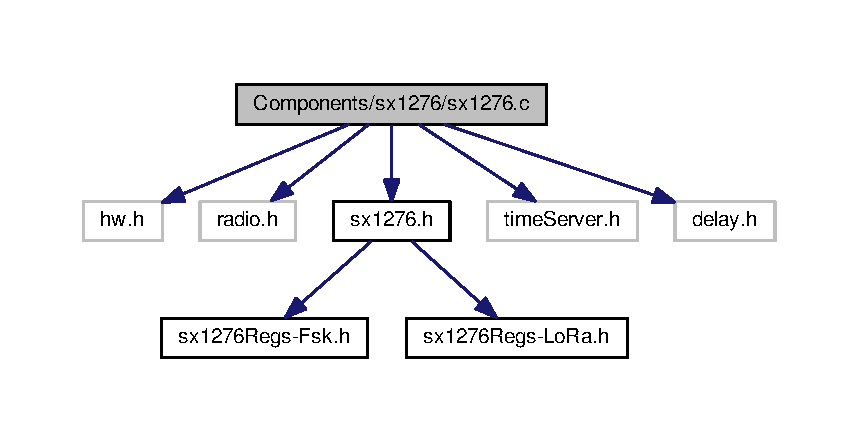
\includegraphics[width=350pt]{sx1276_8c__incl}
\end{center}
\end{figure}
\subsection*{Data Structures}
\begin{DoxyCompactItemize}
\item 
struct \hyperlink{structRadioRegisters__t}{Radio\+Registers\+\_\+t}
\item 
struct \hyperlink{structFskBandwidth__t}{Fsk\+Bandwidth\+\_\+t}
\end{DoxyCompactItemize}
\subsection*{Macros}
\begin{DoxyCompactItemize}
\item 
\#define \hyperlink{sx1276_8c_ab77d55822a59f8bf947a409624084335}{R\+S\+S\+I\+\_\+\+O\+F\+F\+S\+E\+T\+\_\+\+LF}~-\/164
\item 
\#define \hyperlink{sx1276_8c_ab5dc23476160340984a003c7a7ab9ef6}{R\+S\+S\+I\+\_\+\+O\+F\+F\+S\+E\+T\+\_\+\+HF}~-\/157
\end{DoxyCompactItemize}
\subsection*{Functions}
\begin{DoxyCompactItemize}
\item 
void \hyperlink{sx1276_8c_a593daed5ce70e7cb25545345e547816b}{S\+X1276\+Reset} (void)
\begin{DoxyCompactList}\small\item\em Resets the S\+X1276. \end{DoxyCompactList}\item 
void \hyperlink{sx1276_8c_a4aea9f6f1070dfd4e4b73bb5ddc1fe38}{S\+X1276\+Set\+Tx} (uint32\+\_\+t timeout)
\begin{DoxyCompactList}\small\item\em Sets the S\+X1276 in transmission mode for the given time. \end{DoxyCompactList}\item 
void \hyperlink{sx1276_8c_a6bb158ae216d4a685695ce5db5f2205f}{S\+X1276\+Write\+Fifo} (uint8\+\_\+t $\ast$buffer, uint8\+\_\+t size)
\begin{DoxyCompactList}\small\item\em Writes the buffer contents to the S\+X1276 F\+I\+FO. \end{DoxyCompactList}\item 
void \hyperlink{sx1276_8c_acb9479ed4e6f071c82908a6d53c3b08e}{S\+X1276\+Read\+Fifo} (uint8\+\_\+t $\ast$buffer, uint8\+\_\+t size)
\begin{DoxyCompactList}\small\item\em Reads the contents of the S\+X1276 F\+I\+FO. \end{DoxyCompactList}\item 
void \hyperlink{sx1276_8c_aaaac2e0d7b5bd63fabf38a235d27a452}{S\+X1276\+Set\+Op\+Mode} (uint8\+\_\+t op\+Mode)
\begin{DoxyCompactList}\small\item\em Sets the S\+X1276 operating mode. \end{DoxyCompactList}\item 
void \hyperlink{sx1276_8c_a51cff5becabc1485224d53133f99e0e4}{S\+X1276\+On\+Dio0\+Irq} (void)
\begin{DoxyCompactList}\small\item\em D\+IO 0 I\+RQ callback. \end{DoxyCompactList}\item 
void \hyperlink{sx1276_8c_a9b73d7de11f1d4325b0780938d6328fe}{S\+X1276\+On\+Dio1\+Irq} (void)
\begin{DoxyCompactList}\small\item\em D\+IO 1 I\+RQ callback. \end{DoxyCompactList}\item 
void \hyperlink{sx1276_8c_a6be9c1a3560cc9d8bc746dcb82f5d8ea}{S\+X1276\+On\+Dio2\+Irq} (void)
\begin{DoxyCompactList}\small\item\em D\+IO 2 I\+RQ callback. \end{DoxyCompactList}\item 
void \hyperlink{sx1276_8c_a1aeb3fdb6059d033cb07e0d158a3a933}{S\+X1276\+On\+Dio3\+Irq} (void)
\begin{DoxyCompactList}\small\item\em D\+IO 3 I\+RQ callback. \end{DoxyCompactList}\item 
void \hyperlink{sx1276_8c_a5d39e1d81e8496cad939f062d933015c}{S\+X1276\+On\+Dio4\+Irq} (void)
\begin{DoxyCompactList}\small\item\em D\+IO 4 I\+RQ callback. \end{DoxyCompactList}\item 
void \hyperlink{sx1276_8c_aac41025b284e7e872cecfe88667c0aaa}{S\+X1276\+On\+Dio5\+Irq} (void)
\begin{DoxyCompactList}\small\item\em D\+IO 5 I\+RQ callback. \end{DoxyCompactList}\item 
void \hyperlink{sx1276_8c_a3eda1c409a0269313a079389593d75cb}{S\+X1276\+On\+Timeout\+Irq} (void)
\begin{DoxyCompactList}\small\item\em Tx \& Rx timeout timer callback. \end{DoxyCompactList}\item 
void \hyperlink{sx1276_8c_afad8cc2a5afd223af9eba509bfaa15f4}{S\+X1276\+Board\+Init} (\hyperlink{sx1276_8h_ad4ece8886feb1126f7cf786676572610}{Lo\+Ra\+Board\+Callback\+\_\+t} $\ast$callbacks)
\item 
uint32\+\_\+t \hyperlink{sx1276_8c_a19a9ddff3f878b85e42c7571485fe3c8}{S\+X1276\+Init} (Radio\+Events\+\_\+t $\ast$events)
\begin{DoxyCompactList}\small\item\em Initializes the radio. \end{DoxyCompactList}\item 
Radio\+State\+\_\+t \hyperlink{sx1276_8c_ad70a0b1db3593630b1124653b6374944}{S\+X1276\+Get\+Status} (void)
\item 
void \hyperlink{sx1276_8c_a00768e908043081bc32cb83913192f7f}{S\+X1276\+Set\+Channel} (uint32\+\_\+t freq)
\begin{DoxyCompactList}\small\item\em Sets the channel configuration. \end{DoxyCompactList}\item 
bool \hyperlink{sx1276_8c_a29f26f7258f8fcd5c27800295639d7c7}{S\+X1276\+Is\+Channel\+Free} (Radio\+Modems\+\_\+t modem, uint32\+\_\+t freq, int16\+\_\+t rssi\+Thresh, uint32\+\_\+t max\+Carrier\+Sense\+Time)
\begin{DoxyCompactList}\small\item\em Checks if the channel is free for the given time. \end{DoxyCompactList}\item 
uint32\+\_\+t \hyperlink{sx1276_8c_a9ba39c96b8e339b06dd24543920fd2f7}{S\+X1276\+Random} (void)
\begin{DoxyCompactList}\small\item\em Generates a 32 bits random value based on the R\+S\+SI readings. \end{DoxyCompactList}\item 
void \hyperlink{sx1276_8c_a6a66ceb9e18a33aaff10d384fa493cf8}{S\+X1276\+Set\+Rx\+Config} (Radio\+Modems\+\_\+t modem, uint32\+\_\+t bandwidth, uint32\+\_\+t datarate, uint8\+\_\+t coderate, uint32\+\_\+t bandwidth\+Afc, uint16\+\_\+t preamble\+Len, uint16\+\_\+t symb\+Timeout, bool fix\+Len, uint8\+\_\+t payload\+Len, bool crc\+On, bool freq\+Hop\+On, uint8\+\_\+t hop\+Period, bool iq\+Inverted, bool rx\+Continuous)
\begin{DoxyCompactList}\small\item\em Sets the reception parameters. \end{DoxyCompactList}\item 
void \hyperlink{sx1276_8c_a805df2c0c4aa1630eeeb17177a600269}{S\+X1276\+Set\+Tx\+Config} (Radio\+Modems\+\_\+t modem, int8\+\_\+t power, uint32\+\_\+t fdev, uint32\+\_\+t bandwidth, uint32\+\_\+t datarate, uint8\+\_\+t coderate, uint16\+\_\+t preamble\+Len, bool fix\+Len, bool crc\+On, bool freq\+Hop\+On, uint8\+\_\+t hop\+Period, bool iq\+Inverted, uint32\+\_\+t timeout)
\begin{DoxyCompactList}\small\item\em Sets the transmission parameters. \end{DoxyCompactList}\item 
uint32\+\_\+t \hyperlink{sx1276_8c_a2d0bda0e5f9a4cce63284461e356b5e2}{S\+X1276\+Get\+Time\+On\+Air} (Radio\+Modems\+\_\+t modem, uint8\+\_\+t pkt\+Len)
\begin{DoxyCompactList}\small\item\em Computes the packet time on air in ms for the given payload. \end{DoxyCompactList}\item 
void \hyperlink{sx1276_8c_a901a3dcdbf26005e0f3f2def3e3d83b3}{S\+X1276\+Send} (uint8\+\_\+t $\ast$buffer, uint8\+\_\+t size)
\begin{DoxyCompactList}\small\item\em Sends the buffer of size. Prepares the packet to be sent and sets the radio in transmission. \end{DoxyCompactList}\item 
void \hyperlink{sx1276_8c_a32a7b8c477b2f400f96a3255e1ab7620}{S\+X1276\+Set\+Sleep} (void)
\begin{DoxyCompactList}\small\item\em Sets the radio in sleep mode. \end{DoxyCompactList}\item 
void \hyperlink{sx1276_8c_aaef7a98104b400b235ef76de0cfb17df}{S\+X1276\+Set\+Stby} (void)
\begin{DoxyCompactList}\small\item\em Sets the radio in standby mode. \end{DoxyCompactList}\item 
void \hyperlink{sx1276_8c_a8c2df9351fbde83379717dc6f76e5c11}{S\+X1276\+Set\+Rx} (uint32\+\_\+t timeout)
\begin{DoxyCompactList}\small\item\em Sets the radio in reception mode for the given time. \end{DoxyCompactList}\item 
void \hyperlink{sx1276_8c_a9958c574c62b2235c4f3d4d6571854db}{S\+X1276\+Start\+Cad} (void)
\begin{DoxyCompactList}\small\item\em Start a Channel Activity Detection. \end{DoxyCompactList}\item 
void \hyperlink{sx1276_8c_ac77895b054eb64df0ee2fa97061efae8}{S\+X1276\+Set\+Tx\+Continuous\+Wave} (uint32\+\_\+t freq, int8\+\_\+t power, uint16\+\_\+t time)
\begin{DoxyCompactList}\small\item\em Sets the radio in continuous wave transmission mode. \end{DoxyCompactList}\item 
int16\+\_\+t \hyperlink{sx1276_8c_a5741300714435f1dd69084a30031f6e3}{S\+X1276\+Read\+Rssi} (Radio\+Modems\+\_\+t modem)
\begin{DoxyCompactList}\small\item\em Reads the current R\+S\+SI value. \end{DoxyCompactList}\item 
void \hyperlink{sx1276_8c_a8325968bbefefab02537762dd274aa8b}{S\+X1276\+Set\+Modem} (Radio\+Modems\+\_\+t modem)
\begin{DoxyCompactList}\small\item\em Configures the radio with the given modem. \end{DoxyCompactList}\item 
void \hyperlink{sx1276_8c_a77f5d37bad59c99a14637f1eee273edc}{S\+X1276\+Write} (uint8\+\_\+t addr, uint8\+\_\+t data)
\begin{DoxyCompactList}\small\item\em Writes the radio register at the specified address. \end{DoxyCompactList}\item 
uint8\+\_\+t \hyperlink{sx1276_8c_a80f15707dfe79d5cd46a9e3d78214522}{S\+X1276\+Read} (uint8\+\_\+t addr)
\begin{DoxyCompactList}\small\item\em Reads the radio register at the specified address. \end{DoxyCompactList}\item 
void \hyperlink{sx1276_8c_a9fbc81d0d84656f61feca7ce78dda70b}{S\+X1276\+Write\+Buffer} (uint8\+\_\+t addr, uint8\+\_\+t $\ast$buffer, uint8\+\_\+t size)
\begin{DoxyCompactList}\small\item\em Writes multiple radio registers starting at address. \end{DoxyCompactList}\item 
void \hyperlink{sx1276_8c_a26a0fc71f16d6bd65124e21b7045e0aa}{S\+X1276\+Read\+Buffer} (uint8\+\_\+t addr, uint8\+\_\+t $\ast$buffer, uint8\+\_\+t size)
\begin{DoxyCompactList}\small\item\em Reads multiple radio registers starting at address. \end{DoxyCompactList}\item 
void \hyperlink{sx1276_8c_aac0bb6d289a1afe69f550cb148f3bac8}{S\+X1276\+Set\+Max\+Payload\+Length} (Radio\+Modems\+\_\+t modem, uint8\+\_\+t max)
\begin{DoxyCompactList}\small\item\em Sets the maximum payload length. \end{DoxyCompactList}\item 
void \hyperlink{sx1276_8c_a8acacaf2d3e05a712a90f587d1908c6c}{S\+X1276\+Set\+Public\+Network} (bool enable)
\begin{DoxyCompactList}\small\item\em Sets the network to public or private. Updates the sync byte. \end{DoxyCompactList}\item 
uint32\+\_\+t \hyperlink{sx1276_8c_a9b6e3fa7bd90fa2dce95ef4d00db7bfe}{S\+X1276\+Get\+Radio\+Wake\+Up\+Time} (void)
\begin{DoxyCompactList}\small\item\em Service to get the radio wake-\/up time. \end{DoxyCompactList}\end{DoxyCompactItemize}
\subsection*{Variables}
\begin{DoxyCompactItemize}
\item 
const \hyperlink{structRadioRegisters__t}{Radio\+Registers\+\_\+t} \hyperlink{sx1276_8c_a85205d43e6b6ad129adfd3f7bb098717}{Radio\+Regs\+Init} \mbox{[}$\,$\mbox{]} = \hyperlink{sx1276_8h_abef7202d2ca987f0fe762a046d5cec52}{R\+A\+D\+I\+O\+\_\+\+I\+N\+I\+T\+\_\+\+R\+E\+G\+I\+S\+T\+E\+R\+S\+\_\+\+V\+A\+L\+UE}
\item 
const \hyperlink{structFskBandwidth__t}{Fsk\+Bandwidth\+\_\+t} \hyperlink{sx1276_8c_a94bd7c9b8d0c4dcb1fc8e9ea69f339fd}{Fsk\+Bandwidths} \mbox{[}$\,$\mbox{]}
\item 
\hyperlink{sx1276_8h_acf7f83d7d25c85897b88fcdc94345e56}{S\+X1276\+\_\+t} \hyperlink{sx1276_8c_a91a81a798b3d849e2cc114c18bf9c5cc}{S\+X1276}
\item 
\hyperlink{sx1276_8h_af462584f307238535daaea42f6ce791c}{Dio\+Irq\+Handler} $\ast$ \hyperlink{sx1276_8c_a54dad26405aa74d20ad277910373da2f}{Dio\+Irq} \mbox{[}$\,$\mbox{]}
\item 
Timer\+Event\+\_\+t \hyperlink{sx1276_8c_a7dfcad4f3c97547289d6550410bf81f4}{Tx\+Timeout\+Timer}
\item 
Timer\+Event\+\_\+t \hyperlink{sx1276_8c_aee89c92e5cb79fd352b43dc60505abcd}{Rx\+Timeout\+Timer}
\item 
Timer\+Event\+\_\+t \hyperlink{sx1276_8c_ae87c84654f83ec000c8f6d373982ab97}{Rx\+Timeout\+Sync\+Word}
\end{DoxyCompactItemize}


\subsection{Macro Definition Documentation}
\mbox{\Hypertarget{sx1276_8c_ab5dc23476160340984a003c7a7ab9ef6}\label{sx1276_8c_ab5dc23476160340984a003c7a7ab9ef6}} 
\index{sx1276.\+c@{sx1276.\+c}!R\+S\+S\+I\+\_\+\+O\+F\+F\+S\+E\+T\+\_\+\+HF@{R\+S\+S\+I\+\_\+\+O\+F\+F\+S\+E\+T\+\_\+\+HF}}
\index{R\+S\+S\+I\+\_\+\+O\+F\+F\+S\+E\+T\+\_\+\+HF@{R\+S\+S\+I\+\_\+\+O\+F\+F\+S\+E\+T\+\_\+\+HF}!sx1276.\+c@{sx1276.\+c}}
\subsubsection{\texorpdfstring{R\+S\+S\+I\+\_\+\+O\+F\+F\+S\+E\+T\+\_\+\+HF}{RSSI\_OFFSET\_HF}}
{\footnotesize\ttfamily \#define R\+S\+S\+I\+\_\+\+O\+F\+F\+S\+E\+T\+\_\+\+HF~-\/157}

\mbox{\Hypertarget{sx1276_8c_ab77d55822a59f8bf947a409624084335}\label{sx1276_8c_ab77d55822a59f8bf947a409624084335}} 
\index{sx1276.\+c@{sx1276.\+c}!R\+S\+S\+I\+\_\+\+O\+F\+F\+S\+E\+T\+\_\+\+LF@{R\+S\+S\+I\+\_\+\+O\+F\+F\+S\+E\+T\+\_\+\+LF}}
\index{R\+S\+S\+I\+\_\+\+O\+F\+F\+S\+E\+T\+\_\+\+LF@{R\+S\+S\+I\+\_\+\+O\+F\+F\+S\+E\+T\+\_\+\+LF}!sx1276.\+c@{sx1276.\+c}}
\subsubsection{\texorpdfstring{R\+S\+S\+I\+\_\+\+O\+F\+F\+S\+E\+T\+\_\+\+LF}{RSSI\_OFFSET\_LF}}
{\footnotesize\ttfamily \#define R\+S\+S\+I\+\_\+\+O\+F\+F\+S\+E\+T\+\_\+\+LF~-\/164}

Constant values need to compute the R\+S\+SI value 

\subsection{Function Documentation}
\mbox{\Hypertarget{sx1276_8c_afad8cc2a5afd223af9eba509bfaa15f4}\label{sx1276_8c_afad8cc2a5afd223af9eba509bfaa15f4}} 
\index{sx1276.\+c@{sx1276.\+c}!S\+X1276\+Board\+Init@{S\+X1276\+Board\+Init}}
\index{S\+X1276\+Board\+Init@{S\+X1276\+Board\+Init}!sx1276.\+c@{sx1276.\+c}}
\subsubsection{\texorpdfstring{S\+X1276\+Board\+Init()}{SX1276BoardInit()}}
{\footnotesize\ttfamily void S\+X1276\+Board\+Init (\begin{DoxyParamCaption}\item[{\hyperlink{sx1276_8h_ad4ece8886feb1126f7cf786676572610}{Lo\+Ra\+Board\+Callback\+\_\+t} $\ast$}]{callbacks }\end{DoxyParamCaption})}

============================================================================ \subsection*{Public functions prototypes }\mbox{\Hypertarget{sx1276_8c_a9b6e3fa7bd90fa2dce95ef4d00db7bfe}\label{sx1276_8c_a9b6e3fa7bd90fa2dce95ef4d00db7bfe}} 
\index{sx1276.\+c@{sx1276.\+c}!S\+X1276\+Get\+Radio\+Wake\+Up\+Time@{S\+X1276\+Get\+Radio\+Wake\+Up\+Time}}
\index{S\+X1276\+Get\+Radio\+Wake\+Up\+Time@{S\+X1276\+Get\+Radio\+Wake\+Up\+Time}!sx1276.\+c@{sx1276.\+c}}
\subsubsection{\texorpdfstring{S\+X1276\+Get\+Radio\+Wake\+Up\+Time()}{SX1276GetRadioWakeUpTime()}}
{\footnotesize\ttfamily uint32\+\_\+t S\+X1276\+Get\+Radio\+Wake\+Up\+Time (\begin{DoxyParamCaption}\item[{void}]{ }\end{DoxyParamCaption})}



Service to get the radio wake-\/up time. 


\begin{DoxyRetVals}{Return values}
{\em Value} & of the radio wake-\/up time. \\
\hline
\end{DoxyRetVals}
\mbox{\Hypertarget{sx1276_8c_ad70a0b1db3593630b1124653b6374944}\label{sx1276_8c_ad70a0b1db3593630b1124653b6374944}} 
\index{sx1276.\+c@{sx1276.\+c}!S\+X1276\+Get\+Status@{S\+X1276\+Get\+Status}}
\index{S\+X1276\+Get\+Status@{S\+X1276\+Get\+Status}!sx1276.\+c@{sx1276.\+c}}
\subsubsection{\texorpdfstring{S\+X1276\+Get\+Status()}{SX1276GetStatus()}}
{\footnotesize\ttfamily Radio\+State\+\_\+t S\+X1276\+Get\+Status (\begin{DoxyParamCaption}\item[{void}]{ }\end{DoxyParamCaption})}

Return current radio status


\begin{DoxyParams}{Parameters}
{\em status} & Radio status.\mbox{[}R\+F\+\_\+\+I\+D\+LE, R\+F\+\_\+\+R\+X\+\_\+\+R\+U\+N\+N\+I\+NG, R\+F\+\_\+\+T\+X\+\_\+\+R\+U\+N\+N\+I\+NG\mbox{]} \\
\hline
\end{DoxyParams}
\mbox{\Hypertarget{sx1276_8c_a2d0bda0e5f9a4cce63284461e356b5e2}\label{sx1276_8c_a2d0bda0e5f9a4cce63284461e356b5e2}} 
\index{sx1276.\+c@{sx1276.\+c}!S\+X1276\+Get\+Time\+On\+Air@{S\+X1276\+Get\+Time\+On\+Air}}
\index{S\+X1276\+Get\+Time\+On\+Air@{S\+X1276\+Get\+Time\+On\+Air}!sx1276.\+c@{sx1276.\+c}}
\subsubsection{\texorpdfstring{S\+X1276\+Get\+Time\+On\+Air()}{SX1276GetTimeOnAir()}}
{\footnotesize\ttfamily uint32\+\_\+t S\+X1276\+Get\+Time\+On\+Air (\begin{DoxyParamCaption}\item[{Radio\+Modems\+\_\+t}]{modem,  }\item[{uint8\+\_\+t}]{pkt\+Len }\end{DoxyParamCaption})}



Computes the packet time on air in ms for the given payload. 

Can only be called once Set\+Rx\+Config or Set\+Tx\+Config have been called


\begin{DoxyParams}{Parameters}
{\em \mbox{[}\+I\+N\mbox{]}} & modem Radio modem to be used \mbox{[}0\+: F\+SK, 1\+: Lo\+Ra\mbox{]} \\
\hline
{\em \mbox{[}\+I\+N\mbox{]}} & pkt\+Len Packet payload length\\
\hline
\end{DoxyParams}

\begin{DoxyRetVals}{Return values}
{\em air\+Time} & Computed air\+Time (ms) for the given packet payload length \\
\hline
\end{DoxyRetVals}
\mbox{\Hypertarget{sx1276_8c_a19a9ddff3f878b85e42c7571485fe3c8}\label{sx1276_8c_a19a9ddff3f878b85e42c7571485fe3c8}} 
\index{sx1276.\+c@{sx1276.\+c}!S\+X1276\+Init@{S\+X1276\+Init}}
\index{S\+X1276\+Init@{S\+X1276\+Init}!sx1276.\+c@{sx1276.\+c}}
\subsubsection{\texorpdfstring{S\+X1276\+Init()}{SX1276Init()}}
{\footnotesize\ttfamily uint32\+\_\+t S\+X1276\+Init (\begin{DoxyParamCaption}\item[{Radio\+Events\+\_\+t $\ast$}]{events }\end{DoxyParamCaption})}



Initializes the radio. 


\begin{DoxyParams}{Parameters}
{\em \mbox{[}\+I\+N\mbox{]}} & events Structure containing the driver callback functions \\
\hline
{\em \mbox{[}\+O\+U\+T\mbox{]}} & returns the wake up time of the radio and associated board \\
\hline
\end{DoxyParams}
\mbox{\Hypertarget{sx1276_8c_a29f26f7258f8fcd5c27800295639d7c7}\label{sx1276_8c_a29f26f7258f8fcd5c27800295639d7c7}} 
\index{sx1276.\+c@{sx1276.\+c}!S\+X1276\+Is\+Channel\+Free@{S\+X1276\+Is\+Channel\+Free}}
\index{S\+X1276\+Is\+Channel\+Free@{S\+X1276\+Is\+Channel\+Free}!sx1276.\+c@{sx1276.\+c}}
\subsubsection{\texorpdfstring{S\+X1276\+Is\+Channel\+Free()}{SX1276IsChannelFree()}}
{\footnotesize\ttfamily bool S\+X1276\+Is\+Channel\+Free (\begin{DoxyParamCaption}\item[{Radio\+Modems\+\_\+t}]{modem,  }\item[{uint32\+\_\+t}]{freq,  }\item[{int16\+\_\+t}]{rssi\+Thresh,  }\item[{uint32\+\_\+t}]{max\+Carrier\+Sense\+Time }\end{DoxyParamCaption})}



Checks if the channel is free for the given time. 


\begin{DoxyParams}{Parameters}
{\em \mbox{[}\+I\+N\mbox{]}} & modem Radio modem to be used \mbox{[}0\+: F\+SK, 1\+: Lo\+Ra\mbox{]} \\
\hline
{\em \mbox{[}\+I\+N\mbox{]}} & freq Channel RF frequency \\
\hline
{\em \mbox{[}\+I\+N\mbox{]}} & rssi\+Thresh R\+S\+SI threshold \\
\hline
{\em \mbox{[}\+I\+N\mbox{]}} & max\+Carrier\+Sense\+Time Max time while the R\+S\+SI is measured\\
\hline
\end{DoxyParams}

\begin{DoxyRetVals}{Return values}
{\em is\+Free} & \mbox{[}true\+: Channel is free, false\+: Channel is not free\mbox{]} \\
\hline
\end{DoxyRetVals}
\mbox{\Hypertarget{sx1276_8c_a51cff5becabc1485224d53133f99e0e4}\label{sx1276_8c_a51cff5becabc1485224d53133f99e0e4}} 
\index{sx1276.\+c@{sx1276.\+c}!S\+X1276\+On\+Dio0\+Irq@{S\+X1276\+On\+Dio0\+Irq}}
\index{S\+X1276\+On\+Dio0\+Irq@{S\+X1276\+On\+Dio0\+Irq}!sx1276.\+c@{sx1276.\+c}}
\subsubsection{\texorpdfstring{S\+X1276\+On\+Dio0\+Irq()}{SX1276OnDio0Irq()}}
{\footnotesize\ttfamily void S\+X1276\+On\+Dio0\+Irq (\begin{DoxyParamCaption}\item[{void}]{ }\end{DoxyParamCaption})}



D\+IO 0 I\+RQ callback. 

\mbox{\Hypertarget{sx1276_8c_a9b73d7de11f1d4325b0780938d6328fe}\label{sx1276_8c_a9b73d7de11f1d4325b0780938d6328fe}} 
\index{sx1276.\+c@{sx1276.\+c}!S\+X1276\+On\+Dio1\+Irq@{S\+X1276\+On\+Dio1\+Irq}}
\index{S\+X1276\+On\+Dio1\+Irq@{S\+X1276\+On\+Dio1\+Irq}!sx1276.\+c@{sx1276.\+c}}
\subsubsection{\texorpdfstring{S\+X1276\+On\+Dio1\+Irq()}{SX1276OnDio1Irq()}}
{\footnotesize\ttfamily void S\+X1276\+On\+Dio1\+Irq (\begin{DoxyParamCaption}\item[{void}]{ }\end{DoxyParamCaption})}



D\+IO 1 I\+RQ callback. 

\mbox{\Hypertarget{sx1276_8c_a6be9c1a3560cc9d8bc746dcb82f5d8ea}\label{sx1276_8c_a6be9c1a3560cc9d8bc746dcb82f5d8ea}} 
\index{sx1276.\+c@{sx1276.\+c}!S\+X1276\+On\+Dio2\+Irq@{S\+X1276\+On\+Dio2\+Irq}}
\index{S\+X1276\+On\+Dio2\+Irq@{S\+X1276\+On\+Dio2\+Irq}!sx1276.\+c@{sx1276.\+c}}
\subsubsection{\texorpdfstring{S\+X1276\+On\+Dio2\+Irq()}{SX1276OnDio2Irq()}}
{\footnotesize\ttfamily void S\+X1276\+On\+Dio2\+Irq (\begin{DoxyParamCaption}\item[{void}]{ }\end{DoxyParamCaption})}



D\+IO 2 I\+RQ callback. 

\mbox{\Hypertarget{sx1276_8c_a1aeb3fdb6059d033cb07e0d158a3a933}\label{sx1276_8c_a1aeb3fdb6059d033cb07e0d158a3a933}} 
\index{sx1276.\+c@{sx1276.\+c}!S\+X1276\+On\+Dio3\+Irq@{S\+X1276\+On\+Dio3\+Irq}}
\index{S\+X1276\+On\+Dio3\+Irq@{S\+X1276\+On\+Dio3\+Irq}!sx1276.\+c@{sx1276.\+c}}
\subsubsection{\texorpdfstring{S\+X1276\+On\+Dio3\+Irq()}{SX1276OnDio3Irq()}}
{\footnotesize\ttfamily void S\+X1276\+On\+Dio3\+Irq (\begin{DoxyParamCaption}\item[{void}]{ }\end{DoxyParamCaption})}



D\+IO 3 I\+RQ callback. 

\mbox{\Hypertarget{sx1276_8c_a5d39e1d81e8496cad939f062d933015c}\label{sx1276_8c_a5d39e1d81e8496cad939f062d933015c}} 
\index{sx1276.\+c@{sx1276.\+c}!S\+X1276\+On\+Dio4\+Irq@{S\+X1276\+On\+Dio4\+Irq}}
\index{S\+X1276\+On\+Dio4\+Irq@{S\+X1276\+On\+Dio4\+Irq}!sx1276.\+c@{sx1276.\+c}}
\subsubsection{\texorpdfstring{S\+X1276\+On\+Dio4\+Irq()}{SX1276OnDio4Irq()}}
{\footnotesize\ttfamily void S\+X1276\+On\+Dio4\+Irq (\begin{DoxyParamCaption}\item[{void}]{ }\end{DoxyParamCaption})}



D\+IO 4 I\+RQ callback. 

\mbox{\Hypertarget{sx1276_8c_aac41025b284e7e872cecfe88667c0aaa}\label{sx1276_8c_aac41025b284e7e872cecfe88667c0aaa}} 
\index{sx1276.\+c@{sx1276.\+c}!S\+X1276\+On\+Dio5\+Irq@{S\+X1276\+On\+Dio5\+Irq}}
\index{S\+X1276\+On\+Dio5\+Irq@{S\+X1276\+On\+Dio5\+Irq}!sx1276.\+c@{sx1276.\+c}}
\subsubsection{\texorpdfstring{S\+X1276\+On\+Dio5\+Irq()}{SX1276OnDio5Irq()}}
{\footnotesize\ttfamily void S\+X1276\+On\+Dio5\+Irq (\begin{DoxyParamCaption}\item[{void}]{ }\end{DoxyParamCaption})}



D\+IO 5 I\+RQ callback. 

\mbox{\Hypertarget{sx1276_8c_a3eda1c409a0269313a079389593d75cb}\label{sx1276_8c_a3eda1c409a0269313a079389593d75cb}} 
\index{sx1276.\+c@{sx1276.\+c}!S\+X1276\+On\+Timeout\+Irq@{S\+X1276\+On\+Timeout\+Irq}}
\index{S\+X1276\+On\+Timeout\+Irq@{S\+X1276\+On\+Timeout\+Irq}!sx1276.\+c@{sx1276.\+c}}
\subsubsection{\texorpdfstring{S\+X1276\+On\+Timeout\+Irq()}{SX1276OnTimeoutIrq()}}
{\footnotesize\ttfamily void S\+X1276\+On\+Timeout\+Irq (\begin{DoxyParamCaption}\item[{void}]{ }\end{DoxyParamCaption})}



Tx \& Rx timeout timer callback. 

\mbox{\Hypertarget{sx1276_8c_a9ba39c96b8e339b06dd24543920fd2f7}\label{sx1276_8c_a9ba39c96b8e339b06dd24543920fd2f7}} 
\index{sx1276.\+c@{sx1276.\+c}!S\+X1276\+Random@{S\+X1276\+Random}}
\index{S\+X1276\+Random@{S\+X1276\+Random}!sx1276.\+c@{sx1276.\+c}}
\subsubsection{\texorpdfstring{S\+X1276\+Random()}{SX1276Random()}}
{\footnotesize\ttfamily uint32\+\_\+t S\+X1276\+Random (\begin{DoxyParamCaption}\item[{void}]{ }\end{DoxyParamCaption})}



Generates a 32 bits random value based on the R\+S\+SI readings. 

\begin{DoxyRemark}{Remarks}
This function sets the radio in Lo\+Ra modem mode and disables all interrupts. After calling this function either S\+X1276\+Set\+Rx\+Config or S\+X1276\+Set\+Tx\+Config functions must be called.
\end{DoxyRemark}

\begin{DoxyRetVals}{Return values}
{\em random\+Value} & 32 bits random value \\
\hline
\end{DoxyRetVals}
\mbox{\Hypertarget{sx1276_8c_a80f15707dfe79d5cd46a9e3d78214522}\label{sx1276_8c_a80f15707dfe79d5cd46a9e3d78214522}} 
\index{sx1276.\+c@{sx1276.\+c}!S\+X1276\+Read@{S\+X1276\+Read}}
\index{S\+X1276\+Read@{S\+X1276\+Read}!sx1276.\+c@{sx1276.\+c}}
\subsubsection{\texorpdfstring{S\+X1276\+Read()}{SX1276Read()}}
{\footnotesize\ttfamily uint8\+\_\+t S\+X1276\+Read (\begin{DoxyParamCaption}\item[{uint8\+\_\+t}]{addr }\end{DoxyParamCaption})}



Reads the radio register at the specified address. 


\begin{DoxyParams}{Parameters}
{\em \mbox{[}\+I\+N\mbox{]}} & addr Register address \\
\hline
\end{DoxyParams}

\begin{DoxyRetVals}{Return values}
{\em data} & Register value \\
\hline
\end{DoxyRetVals}
\mbox{\Hypertarget{sx1276_8c_a26a0fc71f16d6bd65124e21b7045e0aa}\label{sx1276_8c_a26a0fc71f16d6bd65124e21b7045e0aa}} 
\index{sx1276.\+c@{sx1276.\+c}!S\+X1276\+Read\+Buffer@{S\+X1276\+Read\+Buffer}}
\index{S\+X1276\+Read\+Buffer@{S\+X1276\+Read\+Buffer}!sx1276.\+c@{sx1276.\+c}}
\subsubsection{\texorpdfstring{S\+X1276\+Read\+Buffer()}{SX1276ReadBuffer()}}
{\footnotesize\ttfamily void S\+X1276\+Read\+Buffer (\begin{DoxyParamCaption}\item[{uint8\+\_\+t}]{addr,  }\item[{uint8\+\_\+t $\ast$}]{buffer,  }\item[{uint8\+\_\+t}]{size }\end{DoxyParamCaption})}



Reads multiple radio registers starting at address. 


\begin{DoxyParams}{Parameters}
{\em \mbox{[}\+I\+N\mbox{]}} & addr First Radio register address \\
\hline
{\em \mbox{[}\+O\+U\+T\mbox{]}} & buffer Buffer where to copy the registers data \\
\hline
{\em \mbox{[}\+I\+N\mbox{]}} & size Number of registers to be read \\
\hline
\end{DoxyParams}
\mbox{\Hypertarget{sx1276_8c_acb9479ed4e6f071c82908a6d53c3b08e}\label{sx1276_8c_acb9479ed4e6f071c82908a6d53c3b08e}} 
\index{sx1276.\+c@{sx1276.\+c}!S\+X1276\+Read\+Fifo@{S\+X1276\+Read\+Fifo}}
\index{S\+X1276\+Read\+Fifo@{S\+X1276\+Read\+Fifo}!sx1276.\+c@{sx1276.\+c}}
\subsubsection{\texorpdfstring{S\+X1276\+Read\+Fifo()}{SX1276ReadFifo()}}
{\footnotesize\ttfamily void S\+X1276\+Read\+Fifo (\begin{DoxyParamCaption}\item[{uint8\+\_\+t $\ast$}]{buffer,  }\item[{uint8\+\_\+t}]{size }\end{DoxyParamCaption})}



Reads the contents of the S\+X1276 F\+I\+FO. 


\begin{DoxyParams}{Parameters}
{\em \mbox{[}\+O\+U\+T\mbox{]}} & buffer Buffer where to copy the F\+I\+FO read data. \\
\hline
{\em \mbox{[}\+I\+N\mbox{]}} & size Number of bytes to be read from the F\+I\+FO \\
\hline
\end{DoxyParams}
\mbox{\Hypertarget{sx1276_8c_a5741300714435f1dd69084a30031f6e3}\label{sx1276_8c_a5741300714435f1dd69084a30031f6e3}} 
\index{sx1276.\+c@{sx1276.\+c}!S\+X1276\+Read\+Rssi@{S\+X1276\+Read\+Rssi}}
\index{S\+X1276\+Read\+Rssi@{S\+X1276\+Read\+Rssi}!sx1276.\+c@{sx1276.\+c}}
\subsubsection{\texorpdfstring{S\+X1276\+Read\+Rssi()}{SX1276ReadRssi()}}
{\footnotesize\ttfamily int16\+\_\+t S\+X1276\+Read\+Rssi (\begin{DoxyParamCaption}\item[{Radio\+Modems\+\_\+t}]{modem }\end{DoxyParamCaption})}



Reads the current R\+S\+SI value. 


\begin{DoxyRetVals}{Return values}
{\em rssi\+Value} & Current R\+S\+SI value in \mbox{[}d\+Bm\mbox{]} \\
\hline
\end{DoxyRetVals}
\mbox{\Hypertarget{sx1276_8c_a593daed5ce70e7cb25545345e547816b}\label{sx1276_8c_a593daed5ce70e7cb25545345e547816b}} 
\index{sx1276.\+c@{sx1276.\+c}!S\+X1276\+Reset@{S\+X1276\+Reset}}
\index{S\+X1276\+Reset@{S\+X1276\+Reset}!sx1276.\+c@{sx1276.\+c}}
\subsubsection{\texorpdfstring{S\+X1276\+Reset()}{SX1276Reset()}}
{\footnotesize\ttfamily void S\+X1276\+Reset (\begin{DoxyParamCaption}\item[{void}]{ }\end{DoxyParamCaption})}



Resets the S\+X1276. 

\mbox{\Hypertarget{sx1276_8c_a901a3dcdbf26005e0f3f2def3e3d83b3}\label{sx1276_8c_a901a3dcdbf26005e0f3f2def3e3d83b3}} 
\index{sx1276.\+c@{sx1276.\+c}!S\+X1276\+Send@{S\+X1276\+Send}}
\index{S\+X1276\+Send@{S\+X1276\+Send}!sx1276.\+c@{sx1276.\+c}}
\subsubsection{\texorpdfstring{S\+X1276\+Send()}{SX1276Send()}}
{\footnotesize\ttfamily void S\+X1276\+Send (\begin{DoxyParamCaption}\item[{uint8\+\_\+t $\ast$}]{buffer,  }\item[{uint8\+\_\+t}]{size }\end{DoxyParamCaption})}



Sends the buffer of size. Prepares the packet to be sent and sets the radio in transmission. 


\begin{DoxyParams}{Parameters}
{\em \mbox{[}\+I\+N\mbox{]}} & buffer Buffer pointer \\
\hline
{\em \mbox{[}\+I\+N\mbox{]}} & size Buffer size \\
\hline
\end{DoxyParams}
\mbox{\Hypertarget{sx1276_8c_a00768e908043081bc32cb83913192f7f}\label{sx1276_8c_a00768e908043081bc32cb83913192f7f}} 
\index{sx1276.\+c@{sx1276.\+c}!S\+X1276\+Set\+Channel@{S\+X1276\+Set\+Channel}}
\index{S\+X1276\+Set\+Channel@{S\+X1276\+Set\+Channel}!sx1276.\+c@{sx1276.\+c}}
\subsubsection{\texorpdfstring{S\+X1276\+Set\+Channel()}{SX1276SetChannel()}}
{\footnotesize\ttfamily void S\+X1276\+Set\+Channel (\begin{DoxyParamCaption}\item[{uint32\+\_\+t}]{freq }\end{DoxyParamCaption})}



Sets the channel configuration. 


\begin{DoxyParams}{Parameters}
{\em \mbox{[}\+I\+N\mbox{]}} & freq Channel RF frequency \\
\hline
\end{DoxyParams}
\mbox{\Hypertarget{sx1276_8c_aac0bb6d289a1afe69f550cb148f3bac8}\label{sx1276_8c_aac0bb6d289a1afe69f550cb148f3bac8}} 
\index{sx1276.\+c@{sx1276.\+c}!S\+X1276\+Set\+Max\+Payload\+Length@{S\+X1276\+Set\+Max\+Payload\+Length}}
\index{S\+X1276\+Set\+Max\+Payload\+Length@{S\+X1276\+Set\+Max\+Payload\+Length}!sx1276.\+c@{sx1276.\+c}}
\subsubsection{\texorpdfstring{S\+X1276\+Set\+Max\+Payload\+Length()}{SX1276SetMaxPayloadLength()}}
{\footnotesize\ttfamily void S\+X1276\+Set\+Max\+Payload\+Length (\begin{DoxyParamCaption}\item[{Radio\+Modems\+\_\+t}]{modem,  }\item[{uint8\+\_\+t}]{max }\end{DoxyParamCaption})}



Sets the maximum payload length. 


\begin{DoxyParams}{Parameters}
{\em \mbox{[}\+I\+N\mbox{]}} & modem Radio modem to be used \mbox{[}0\+: F\+SK, 1\+: Lo\+Ra\mbox{]} \\
\hline
{\em \mbox{[}\+I\+N\mbox{]}} & max Maximum payload length in bytes \\
\hline
\end{DoxyParams}
\mbox{\Hypertarget{sx1276_8c_a8325968bbefefab02537762dd274aa8b}\label{sx1276_8c_a8325968bbefefab02537762dd274aa8b}} 
\index{sx1276.\+c@{sx1276.\+c}!S\+X1276\+Set\+Modem@{S\+X1276\+Set\+Modem}}
\index{S\+X1276\+Set\+Modem@{S\+X1276\+Set\+Modem}!sx1276.\+c@{sx1276.\+c}}
\subsubsection{\texorpdfstring{S\+X1276\+Set\+Modem()}{SX1276SetModem()}}
{\footnotesize\ttfamily void S\+X1276\+Set\+Modem (\begin{DoxyParamCaption}\item[{Radio\+Modems\+\_\+t}]{modem }\end{DoxyParamCaption})}



Configures the radio with the given modem. 


\begin{DoxyParams}{Parameters}
{\em \mbox{[}\+I\+N\mbox{]}} & modem Modem to be used \mbox{[}0\+: F\+SK, 1\+: Lo\+Ra\mbox{]} \\
\hline
\end{DoxyParams}
\mbox{\Hypertarget{sx1276_8c_aaaac2e0d7b5bd63fabf38a235d27a452}\label{sx1276_8c_aaaac2e0d7b5bd63fabf38a235d27a452}} 
\index{sx1276.\+c@{sx1276.\+c}!S\+X1276\+Set\+Op\+Mode@{S\+X1276\+Set\+Op\+Mode}}
\index{S\+X1276\+Set\+Op\+Mode@{S\+X1276\+Set\+Op\+Mode}!sx1276.\+c@{sx1276.\+c}}
\subsubsection{\texorpdfstring{S\+X1276\+Set\+Op\+Mode()}{SX1276SetOpMode()}}
{\footnotesize\ttfamily void S\+X1276\+Set\+Op\+Mode (\begin{DoxyParamCaption}\item[{uint8\+\_\+t}]{op\+Mode }\end{DoxyParamCaption})}



Sets the S\+X1276 operating mode. 


\begin{DoxyParams}{Parameters}
{\em \mbox{[}\+I\+N\mbox{]}} & op\+Mode New operating mode \\
\hline
\end{DoxyParams}
\mbox{\Hypertarget{sx1276_8c_a8acacaf2d3e05a712a90f587d1908c6c}\label{sx1276_8c_a8acacaf2d3e05a712a90f587d1908c6c}} 
\index{sx1276.\+c@{sx1276.\+c}!S\+X1276\+Set\+Public\+Network@{S\+X1276\+Set\+Public\+Network}}
\index{S\+X1276\+Set\+Public\+Network@{S\+X1276\+Set\+Public\+Network}!sx1276.\+c@{sx1276.\+c}}
\subsubsection{\texorpdfstring{S\+X1276\+Set\+Public\+Network()}{SX1276SetPublicNetwork()}}
{\footnotesize\ttfamily void S\+X1276\+Set\+Public\+Network (\begin{DoxyParamCaption}\item[{bool}]{enable }\end{DoxyParamCaption})}



Sets the network to public or private. Updates the sync byte. 

\begin{DoxyRemark}{Remarks}
Applies to Lo\+Ra modem only
\end{DoxyRemark}

\begin{DoxyParams}{Parameters}
{\em \mbox{[}\+I\+N\mbox{]}} & enable if true, it enables a public network \\
\hline
\end{DoxyParams}
\mbox{\Hypertarget{sx1276_8c_a8c2df9351fbde83379717dc6f76e5c11}\label{sx1276_8c_a8c2df9351fbde83379717dc6f76e5c11}} 
\index{sx1276.\+c@{sx1276.\+c}!S\+X1276\+Set\+Rx@{S\+X1276\+Set\+Rx}}
\index{S\+X1276\+Set\+Rx@{S\+X1276\+Set\+Rx}!sx1276.\+c@{sx1276.\+c}}
\subsubsection{\texorpdfstring{S\+X1276\+Set\+Rx()}{SX1276SetRx()}}
{\footnotesize\ttfamily void S\+X1276\+Set\+Rx (\begin{DoxyParamCaption}\item[{uint32\+\_\+t}]{timeout }\end{DoxyParamCaption})}



Sets the radio in reception mode for the given time. 


\begin{DoxyParams}{Parameters}
{\em \mbox{[}\+I\+N\mbox{]}} & timeout Reception timeout \mbox{[}ms\mbox{]} \mbox{[}0\+: continuous, others timeout\mbox{]} \\
\hline
\end{DoxyParams}
\mbox{\Hypertarget{sx1276_8c_a6a66ceb9e18a33aaff10d384fa493cf8}\label{sx1276_8c_a6a66ceb9e18a33aaff10d384fa493cf8}} 
\index{sx1276.\+c@{sx1276.\+c}!S\+X1276\+Set\+Rx\+Config@{S\+X1276\+Set\+Rx\+Config}}
\index{S\+X1276\+Set\+Rx\+Config@{S\+X1276\+Set\+Rx\+Config}!sx1276.\+c@{sx1276.\+c}}
\subsubsection{\texorpdfstring{S\+X1276\+Set\+Rx\+Config()}{SX1276SetRxConfig()}}
{\footnotesize\ttfamily void S\+X1276\+Set\+Rx\+Config (\begin{DoxyParamCaption}\item[{Radio\+Modems\+\_\+t}]{modem,  }\item[{uint32\+\_\+t}]{bandwidth,  }\item[{uint32\+\_\+t}]{datarate,  }\item[{uint8\+\_\+t}]{coderate,  }\item[{uint32\+\_\+t}]{bandwidth\+Afc,  }\item[{uint16\+\_\+t}]{preamble\+Len,  }\item[{uint16\+\_\+t}]{symb\+Timeout,  }\item[{bool}]{fix\+Len,  }\item[{uint8\+\_\+t}]{payload\+Len,  }\item[{bool}]{crc\+On,  }\item[{bool}]{freq\+Hop\+On,  }\item[{uint8\+\_\+t}]{hop\+Period,  }\item[{bool}]{iq\+Inverted,  }\item[{bool}]{rx\+Continuous }\end{DoxyParamCaption})}



Sets the reception parameters. 

\begin{DoxyRemark}{Remarks}
When using Lo\+Ra modem only bandwidths 125, 250 and 500 k\+Hz are supported
\end{DoxyRemark}

\begin{DoxyParams}{Parameters}
{\em \mbox{[}\+I\+N\mbox{]}} & modem Radio modem to be used \mbox{[}0\+: F\+SK, 1\+: Lo\+Ra\mbox{]} \\
\hline
{\em \mbox{[}\+I\+N\mbox{]}} & bandwidth Sets the bandwidth F\+SK \+: $>$= 2600 and $<$= 250000 Hz Lo\+Ra\+: \mbox{[}0\+: 125 k\+Hz, 1\+: 250 k\+Hz, 2\+: 500 k\+Hz, 3\+: Reserved\mbox{]} \\
\hline
{\em \mbox{[}\+I\+N\mbox{]}} & datarate Sets the Datarate F\+SK \+: 600..300000 bits/s Lo\+Ra\+: \mbox{[}6\+: 64, 7\+: 128, 8\+: 256, 9\+: 512, 10\+: 1024, 11\+: 2048, 12\+: 4096 chips\mbox{]} \\
\hline
{\em \mbox{[}\+I\+N\mbox{]}} & coderate Sets the coding rate (Lo\+Ra only) F\+SK \+: N/A ( set to 0 ) Lo\+Ra\+: \mbox{[}1\+: 4/5, 2\+: 4/6, 3\+: 4/7, 4\+: 4/8\mbox{]} \\
\hline
{\em \mbox{[}\+I\+N\mbox{]}} & bandwidth\+Afc Sets the A\+FC Bandwidth (F\+SK only) F\+SK \+: $>$= 2600 and $<$= 250000 Hz Lo\+Ra\+: N/A ( set to 0 ) \\
\hline
{\em \mbox{[}\+I\+N\mbox{]}} & preamble\+Len Sets the Preamble length F\+SK \+: Number of bytes Lo\+Ra\+: Length in symbols (the hardware adds 4 more symbols) \\
\hline
{\em \mbox{[}\+I\+N\mbox{]}} & symb\+Timeout Sets the Rx\+Single timeout value F\+SK \+: timeout number of bytes Lo\+Ra\+: timeout in symbols \\
\hline
{\em \mbox{[}\+I\+N\mbox{]}} & fix\+Len Fixed length packets \mbox{[}0\+: variable, 1\+: fixed\mbox{]} \\
\hline
{\em \mbox{[}\+I\+N\mbox{]}} & payload\+Len Sets payload length when fixed length is used \\
\hline
{\em \mbox{[}\+I\+N\mbox{]}} & crc\+On Enables/\+Disables the C\+RC \mbox{[}0\+: O\+FF, 1\+: ON\mbox{]} \\
\hline
{\em \mbox{[}\+I\+N\mbox{]}} & freq\+Hop\+On Enables disables the intra-\/packet frequency hopping F\+SK \+: N/A ( set to 0 ) Lo\+Ra\+: \mbox{[}0\+: O\+FF, 1\+: ON\mbox{]} \\
\hline
{\em \mbox{[}\+I\+N\mbox{]}} & hop\+Period Number of symbols between each hop F\+SK \+: N/A ( set to 0 ) Lo\+Ra\+: Number of symbols \\
\hline
{\em \mbox{[}\+I\+N\mbox{]}} & iq\+Inverted Inverts IQ signals (Lo\+Ra only) F\+SK \+: N/A ( set to 0 ) Lo\+Ra\+: \mbox{[}0\+: not inverted, 1\+: inverted\mbox{]} \\
\hline
{\em \mbox{[}\+I\+N\mbox{]}} & rx\+Continuous Sets the reception in continuous mode \mbox{[}false\+: single mode, true\+: continuous mode\mbox{]} \\
\hline
\end{DoxyParams}
\mbox{\Hypertarget{sx1276_8c_a32a7b8c477b2f400f96a3255e1ab7620}\label{sx1276_8c_a32a7b8c477b2f400f96a3255e1ab7620}} 
\index{sx1276.\+c@{sx1276.\+c}!S\+X1276\+Set\+Sleep@{S\+X1276\+Set\+Sleep}}
\index{S\+X1276\+Set\+Sleep@{S\+X1276\+Set\+Sleep}!sx1276.\+c@{sx1276.\+c}}
\subsubsection{\texorpdfstring{S\+X1276\+Set\+Sleep()}{SX1276SetSleep()}}
{\footnotesize\ttfamily void S\+X1276\+Set\+Sleep (\begin{DoxyParamCaption}\item[{void}]{ }\end{DoxyParamCaption})}



Sets the radio in sleep mode. 

\mbox{\Hypertarget{sx1276_8c_aaef7a98104b400b235ef76de0cfb17df}\label{sx1276_8c_aaef7a98104b400b235ef76de0cfb17df}} 
\index{sx1276.\+c@{sx1276.\+c}!S\+X1276\+Set\+Stby@{S\+X1276\+Set\+Stby}}
\index{S\+X1276\+Set\+Stby@{S\+X1276\+Set\+Stby}!sx1276.\+c@{sx1276.\+c}}
\subsubsection{\texorpdfstring{S\+X1276\+Set\+Stby()}{SX1276SetStby()}}
{\footnotesize\ttfamily void S\+X1276\+Set\+Stby (\begin{DoxyParamCaption}\item[{void}]{ }\end{DoxyParamCaption})}



Sets the radio in standby mode. 

\mbox{\Hypertarget{sx1276_8c_a4aea9f6f1070dfd4e4b73bb5ddc1fe38}\label{sx1276_8c_a4aea9f6f1070dfd4e4b73bb5ddc1fe38}} 
\index{sx1276.\+c@{sx1276.\+c}!S\+X1276\+Set\+Tx@{S\+X1276\+Set\+Tx}}
\index{S\+X1276\+Set\+Tx@{S\+X1276\+Set\+Tx}!sx1276.\+c@{sx1276.\+c}}
\subsubsection{\texorpdfstring{S\+X1276\+Set\+Tx()}{SX1276SetTx()}}
{\footnotesize\ttfamily void S\+X1276\+Set\+Tx (\begin{DoxyParamCaption}\item[{uint32\+\_\+t}]{timeout }\end{DoxyParamCaption})}



Sets the S\+X1276 in transmission mode for the given time. 


\begin{DoxyParams}{Parameters}
{\em \mbox{[}\+I\+N\mbox{]}} & timeout Transmission timeout \mbox{[}ms\mbox{]} \mbox{[}0\+: continuous, others timeout\mbox{]} \\
\hline
\end{DoxyParams}
\mbox{\Hypertarget{sx1276_8c_a805df2c0c4aa1630eeeb17177a600269}\label{sx1276_8c_a805df2c0c4aa1630eeeb17177a600269}} 
\index{sx1276.\+c@{sx1276.\+c}!S\+X1276\+Set\+Tx\+Config@{S\+X1276\+Set\+Tx\+Config}}
\index{S\+X1276\+Set\+Tx\+Config@{S\+X1276\+Set\+Tx\+Config}!sx1276.\+c@{sx1276.\+c}}
\subsubsection{\texorpdfstring{S\+X1276\+Set\+Tx\+Config()}{SX1276SetTxConfig()}}
{\footnotesize\ttfamily void S\+X1276\+Set\+Tx\+Config (\begin{DoxyParamCaption}\item[{Radio\+Modems\+\_\+t}]{modem,  }\item[{int8\+\_\+t}]{power,  }\item[{uint32\+\_\+t}]{fdev,  }\item[{uint32\+\_\+t}]{bandwidth,  }\item[{uint32\+\_\+t}]{datarate,  }\item[{uint8\+\_\+t}]{coderate,  }\item[{uint16\+\_\+t}]{preamble\+Len,  }\item[{bool}]{fix\+Len,  }\item[{bool}]{crc\+On,  }\item[{bool}]{freq\+Hop\+On,  }\item[{uint8\+\_\+t}]{hop\+Period,  }\item[{bool}]{iq\+Inverted,  }\item[{uint32\+\_\+t}]{timeout }\end{DoxyParamCaption})}



Sets the transmission parameters. 

\begin{DoxyRemark}{Remarks}
When using Lo\+Ra modem only bandwidths 125, 250 and 500 k\+Hz are supported
\end{DoxyRemark}

\begin{DoxyParams}{Parameters}
{\em \mbox{[}\+I\+N\mbox{]}} & modem Radio modem to be used \mbox{[}0\+: F\+SK, 1\+: Lo\+Ra\mbox{]} \\
\hline
{\em \mbox{[}\+I\+N\mbox{]}} & power Sets the output power \mbox{[}d\+Bm\mbox{]} \\
\hline
{\em \mbox{[}\+I\+N\mbox{]}} & fdev Sets the frequency deviation (F\+SK only) F\+SK \+: \mbox{[}Hz\mbox{]} Lo\+Ra\+: 0 \\
\hline
{\em \mbox{[}\+I\+N\mbox{]}} & bandwidth Sets the bandwidth (Lo\+Ra only) F\+SK \+: 0 Lo\+Ra\+: \mbox{[}0\+: 125 k\+Hz, 1\+: 250 k\+Hz, 2\+: 500 k\+Hz, 3\+: Reserved\mbox{]} \\
\hline
{\em \mbox{[}\+I\+N\mbox{]}} & datarate Sets the Datarate F\+SK \+: 600..300000 bits/s Lo\+Ra\+: \mbox{[}6\+: 64, 7\+: 128, 8\+: 256, 9\+: 512, 10\+: 1024, 11\+: 2048, 12\+: 4096 chips\mbox{]} \\
\hline
{\em \mbox{[}\+I\+N\mbox{]}} & coderate Sets the coding rate (Lo\+Ra only) F\+SK \+: N/A ( set to 0 ) Lo\+Ra\+: \mbox{[}1\+: 4/5, 2\+: 4/6, 3\+: 4/7, 4\+: 4/8\mbox{]} \\
\hline
{\em \mbox{[}\+I\+N\mbox{]}} & preamble\+Len Sets the preamble length F\+SK \+: Number of bytes Lo\+Ra\+: Length in symbols (the hardware adds 4 more symbols) \\
\hline
{\em \mbox{[}\+I\+N\mbox{]}} & fix\+Len Fixed length packets \mbox{[}0\+: variable, 1\+: fixed\mbox{]} \\
\hline
{\em \mbox{[}\+I\+N\mbox{]}} & crc\+On Enables disables the C\+RC \mbox{[}0\+: O\+FF, 1\+: ON\mbox{]} \\
\hline
{\em \mbox{[}\+I\+N\mbox{]}} & freq\+Hop\+On Enables disables the intra-\/packet frequency hopping F\+SK \+: N/A ( set to 0 ) Lo\+Ra\+: \mbox{[}0\+: O\+FF, 1\+: ON\mbox{]} \\
\hline
{\em \mbox{[}\+I\+N\mbox{]}} & hop\+Period Number of symbols between each hop F\+SK \+: N/A ( set to 0 ) Lo\+Ra\+: Number of symbols \\
\hline
{\em \mbox{[}\+I\+N\mbox{]}} & iq\+Inverted Inverts IQ signals (Lo\+Ra only) F\+SK \+: N/A ( set to 0 ) Lo\+Ra\+: \mbox{[}0\+: not inverted, 1\+: inverted\mbox{]} \\
\hline
{\em \mbox{[}\+I\+N\mbox{]}} & timeout Transmission timeout \mbox{[}ms\mbox{]} \\
\hline
\end{DoxyParams}
\mbox{\Hypertarget{sx1276_8c_ac77895b054eb64df0ee2fa97061efae8}\label{sx1276_8c_ac77895b054eb64df0ee2fa97061efae8}} 
\index{sx1276.\+c@{sx1276.\+c}!S\+X1276\+Set\+Tx\+Continuous\+Wave@{S\+X1276\+Set\+Tx\+Continuous\+Wave}}
\index{S\+X1276\+Set\+Tx\+Continuous\+Wave@{S\+X1276\+Set\+Tx\+Continuous\+Wave}!sx1276.\+c@{sx1276.\+c}}
\subsubsection{\texorpdfstring{S\+X1276\+Set\+Tx\+Continuous\+Wave()}{SX1276SetTxContinuousWave()}}
{\footnotesize\ttfamily void S\+X1276\+Set\+Tx\+Continuous\+Wave (\begin{DoxyParamCaption}\item[{uint32\+\_\+t}]{freq,  }\item[{int8\+\_\+t}]{power,  }\item[{uint16\+\_\+t}]{time }\end{DoxyParamCaption})}



Sets the radio in continuous wave transmission mode. 


\begin{DoxyParams}{Parameters}
{\em \mbox{[}\+I\+N\mbox{]}} & freq Channel RF frequency \\
\hline
{\em \mbox{[}\+I\+N\mbox{]}} & power Sets the output power \mbox{[}d\+Bm\mbox{]} \\
\hline
{\em \mbox{[}\+I\+N\mbox{]}} & time Transmission mode timeout \mbox{[}s\mbox{]} \\
\hline
\end{DoxyParams}
\mbox{\Hypertarget{sx1276_8c_a9958c574c62b2235c4f3d4d6571854db}\label{sx1276_8c_a9958c574c62b2235c4f3d4d6571854db}} 
\index{sx1276.\+c@{sx1276.\+c}!S\+X1276\+Start\+Cad@{S\+X1276\+Start\+Cad}}
\index{S\+X1276\+Start\+Cad@{S\+X1276\+Start\+Cad}!sx1276.\+c@{sx1276.\+c}}
\subsubsection{\texorpdfstring{S\+X1276\+Start\+Cad()}{SX1276StartCad()}}
{\footnotesize\ttfamily void S\+X1276\+Start\+Cad (\begin{DoxyParamCaption}\item[{void}]{ }\end{DoxyParamCaption})}



Start a Channel Activity Detection. 

\mbox{\Hypertarget{sx1276_8c_a77f5d37bad59c99a14637f1eee273edc}\label{sx1276_8c_a77f5d37bad59c99a14637f1eee273edc}} 
\index{sx1276.\+c@{sx1276.\+c}!S\+X1276\+Write@{S\+X1276\+Write}}
\index{S\+X1276\+Write@{S\+X1276\+Write}!sx1276.\+c@{sx1276.\+c}}
\subsubsection{\texorpdfstring{S\+X1276\+Write()}{SX1276Write()}}
{\footnotesize\ttfamily void S\+X1276\+Write (\begin{DoxyParamCaption}\item[{uint8\+\_\+t}]{addr,  }\item[{uint8\+\_\+t}]{data }\end{DoxyParamCaption})}



Writes the radio register at the specified address. 


\begin{DoxyParams}{Parameters}
{\em \mbox{[}\+I\+N\mbox{]}} & addr Register address \\
\hline
{\em \mbox{[}\+I\+N\mbox{]}} & data New register value \\
\hline
\end{DoxyParams}
\mbox{\Hypertarget{sx1276_8c_a9fbc81d0d84656f61feca7ce78dda70b}\label{sx1276_8c_a9fbc81d0d84656f61feca7ce78dda70b}} 
\index{sx1276.\+c@{sx1276.\+c}!S\+X1276\+Write\+Buffer@{S\+X1276\+Write\+Buffer}}
\index{S\+X1276\+Write\+Buffer@{S\+X1276\+Write\+Buffer}!sx1276.\+c@{sx1276.\+c}}
\subsubsection{\texorpdfstring{S\+X1276\+Write\+Buffer()}{SX1276WriteBuffer()}}
{\footnotesize\ttfamily void S\+X1276\+Write\+Buffer (\begin{DoxyParamCaption}\item[{uint8\+\_\+t}]{addr,  }\item[{uint8\+\_\+t $\ast$}]{buffer,  }\item[{uint8\+\_\+t}]{size }\end{DoxyParamCaption})}



Writes multiple radio registers starting at address. 


\begin{DoxyParams}{Parameters}
{\em \mbox{[}\+I\+N\mbox{]}} & addr First Radio register address \\
\hline
{\em \mbox{[}\+I\+N\mbox{]}} & buffer Buffer containing the new register\textquotesingle{}s values \\
\hline
{\em \mbox{[}\+I\+N\mbox{]}} & size Number of registers to be written \\
\hline
\end{DoxyParams}
\mbox{\Hypertarget{sx1276_8c_a6bb158ae216d4a685695ce5db5f2205f}\label{sx1276_8c_a6bb158ae216d4a685695ce5db5f2205f}} 
\index{sx1276.\+c@{sx1276.\+c}!S\+X1276\+Write\+Fifo@{S\+X1276\+Write\+Fifo}}
\index{S\+X1276\+Write\+Fifo@{S\+X1276\+Write\+Fifo}!sx1276.\+c@{sx1276.\+c}}
\subsubsection{\texorpdfstring{S\+X1276\+Write\+Fifo()}{SX1276WriteFifo()}}
{\footnotesize\ttfamily void S\+X1276\+Write\+Fifo (\begin{DoxyParamCaption}\item[{uint8\+\_\+t $\ast$}]{buffer,  }\item[{uint8\+\_\+t}]{size }\end{DoxyParamCaption})}



Writes the buffer contents to the S\+X1276 F\+I\+FO. 


\begin{DoxyParams}{Parameters}
{\em \mbox{[}\+I\+N\mbox{]}} & buffer Buffer containing data to be put on the F\+I\+FO. \\
\hline
{\em \mbox{[}\+I\+N\mbox{]}} & size Number of bytes to be written to the F\+I\+FO \\
\hline
\end{DoxyParams}


\subsection{Variable Documentation}
\mbox{\Hypertarget{sx1276_8c_a54dad26405aa74d20ad277910373da2f}\label{sx1276_8c_a54dad26405aa74d20ad277910373da2f}} 
\index{sx1276.\+c@{sx1276.\+c}!Dio\+Irq@{Dio\+Irq}}
\index{Dio\+Irq@{Dio\+Irq}!sx1276.\+c@{sx1276.\+c}}
\subsubsection{\texorpdfstring{Dio\+Irq}{DioIrq}}
{\footnotesize\ttfamily \hyperlink{sx1276_8h_af462584f307238535daaea42f6ce791c}{Dio\+Irq\+Handler}$\ast$ Dio\+Irq\mbox{[}$\,$\mbox{]}}

{\bfseries Initial value\+:}
\begin{DoxyCode}
= \{ \hyperlink{sx1276_8c_a51cff5becabc1485224d53133f99e0e4}{SX1276OnDio0Irq}, \hyperlink{sx1276_8c_a9b73d7de11f1d4325b0780938d6328fe}{SX1276OnDio1Irq},
                            \hyperlink{sx1276_8c_a6be9c1a3560cc9d8bc746dcb82f5d8ea}{SX1276OnDio2Irq}, \hyperlink{sx1276_8c_a1aeb3fdb6059d033cb07e0d158a3a933}{SX1276OnDio3Irq},
                            \hyperlink{sx1276_8c_a5d39e1d81e8496cad939f062d933015c}{SX1276OnDio4Irq}, NULL \}
\end{DoxyCode}
Hardware D\+IO I\+RQ callback initialization \mbox{\Hypertarget{sx1276_8c_a94bd7c9b8d0c4dcb1fc8e9ea69f339fd}\label{sx1276_8c_a94bd7c9b8d0c4dcb1fc8e9ea69f339fd}} 
\index{sx1276.\+c@{sx1276.\+c}!Fsk\+Bandwidths@{Fsk\+Bandwidths}}
\index{Fsk\+Bandwidths@{Fsk\+Bandwidths}!sx1276.\+c@{sx1276.\+c}}
\subsubsection{\texorpdfstring{Fsk\+Bandwidths}{FskBandwidths}}
{\footnotesize\ttfamily const \hyperlink{structFskBandwidth__t}{Fsk\+Bandwidth\+\_\+t} Fsk\+Bandwidths\mbox{[}$\,$\mbox{]}}

{\bfseries Initial value\+:}
\begin{DoxyCode}
=
\{
    \{ 2600  , 0x17 \},
    \{ 3100  , 0x0F \},
    \{ 3900  , 0x07 \},
    \{ 5200  , 0x16 \},
    \{ 6300  , 0x0E \},
    \{ 7800  , 0x06 \},
    \{ 10400 , 0x15 \},
    \{ 12500 , 0x0D \},
    \{ 15600 , 0x05 \},
    \{ 20800 , 0x14 \},
    \{ 25000 , 0x0C \},
    \{ 31300 , 0x04 \},
    \{ 41700 , 0x13 \},
    \{ 50000 , 0x0B \},
    \{ 62500 , 0x03 \},
    \{ 83333 , 0x12 \},
    \{ 100000, 0x0A \},
    \{ 125000, 0x02 \},
    \{ 166700, 0x11 \},
    \{ 200000, 0x09 \},
    \{ 250000, 0x01 \},
    \{ 300000, 0x00 \}, 
\}
\end{DoxyCode}
Precomputed F\+SK bandwidth registers values \mbox{\Hypertarget{sx1276_8c_a85205d43e6b6ad129adfd3f7bb098717}\label{sx1276_8c_a85205d43e6b6ad129adfd3f7bb098717}} 
\index{sx1276.\+c@{sx1276.\+c}!Radio\+Regs\+Init@{Radio\+Regs\+Init}}
\index{Radio\+Regs\+Init@{Radio\+Regs\+Init}!sx1276.\+c@{sx1276.\+c}}
\subsubsection{\texorpdfstring{Radio\+Regs\+Init}{RadioRegsInit}}
{\footnotesize\ttfamily const \hyperlink{structRadioRegisters__t}{Radio\+Registers\+\_\+t} Radio\+Regs\+Init\mbox{[}$\,$\mbox{]} = \hyperlink{sx1276_8h_abef7202d2ca987f0fe762a046d5cec52}{R\+A\+D\+I\+O\+\_\+\+I\+N\+I\+T\+\_\+\+R\+E\+G\+I\+S\+T\+E\+R\+S\+\_\+\+V\+A\+L\+UE}}

Radio hardware registers initialization

\begin{DoxyRemark}{Remarks}
R\+A\+D\+I\+O\+\_\+\+I\+N\+I\+T\+\_\+\+R\+E\+G\+I\+S\+T\+E\+R\+S\+\_\+\+V\+A\+L\+UE is defined in sx1276-\/board.\+h file 
\end{DoxyRemark}
\mbox{\Hypertarget{sx1276_8c_ae87c84654f83ec000c8f6d373982ab97}\label{sx1276_8c_ae87c84654f83ec000c8f6d373982ab97}} 
\index{sx1276.\+c@{sx1276.\+c}!Rx\+Timeout\+Sync\+Word@{Rx\+Timeout\+Sync\+Word}}
\index{Rx\+Timeout\+Sync\+Word@{Rx\+Timeout\+Sync\+Word}!sx1276.\+c@{sx1276.\+c}}
\subsubsection{\texorpdfstring{Rx\+Timeout\+Sync\+Word}{RxTimeoutSyncWord}}
{\footnotesize\ttfamily Timer\+Event\+\_\+t Rx\+Timeout\+Sync\+Word}

\mbox{\Hypertarget{sx1276_8c_aee89c92e5cb79fd352b43dc60505abcd}\label{sx1276_8c_aee89c92e5cb79fd352b43dc60505abcd}} 
\index{sx1276.\+c@{sx1276.\+c}!Rx\+Timeout\+Timer@{Rx\+Timeout\+Timer}}
\index{Rx\+Timeout\+Timer@{Rx\+Timeout\+Timer}!sx1276.\+c@{sx1276.\+c}}
\subsubsection{\texorpdfstring{Rx\+Timeout\+Timer}{RxTimeoutTimer}}
{\footnotesize\ttfamily Timer\+Event\+\_\+t Rx\+Timeout\+Timer}

\mbox{\Hypertarget{sx1276_8c_a91a81a798b3d849e2cc114c18bf9c5cc}\label{sx1276_8c_a91a81a798b3d849e2cc114c18bf9c5cc}} 
\index{sx1276.\+c@{sx1276.\+c}!S\+X1276@{S\+X1276}}
\index{S\+X1276@{S\+X1276}!sx1276.\+c@{sx1276.\+c}}
\subsubsection{\texorpdfstring{S\+X1276}{SX1276}}
{\footnotesize\ttfamily \hyperlink{sx1276_8h_acf7f83d7d25c85897b88fcdc94345e56}{S\+X1276\+\_\+t} S\+X1276}

Radio hardware and global parameters \mbox{\Hypertarget{sx1276_8c_a7dfcad4f3c97547289d6550410bf81f4}\label{sx1276_8c_a7dfcad4f3c97547289d6550410bf81f4}} 
\index{sx1276.\+c@{sx1276.\+c}!Tx\+Timeout\+Timer@{Tx\+Timeout\+Timer}}
\index{Tx\+Timeout\+Timer@{Tx\+Timeout\+Timer}!sx1276.\+c@{sx1276.\+c}}
\subsubsection{\texorpdfstring{Tx\+Timeout\+Timer}{TxTimeoutTimer}}
{\footnotesize\ttfamily Timer\+Event\+\_\+t Tx\+Timeout\+Timer}

Tx and Rx timers 
\hypertarget{sx1276_8h}{}\section{Components/sx1276/sx1276.h File Reference}
\label{sx1276_8h}\index{Components/sx1276/sx1276.\+h@{Components/sx1276/sx1276.\+h}}
{\ttfamily \#include \char`\"{}sx1276\+Regs-\/\+Fsk.\+h\char`\"{}}\newline
{\ttfamily \#include \char`\"{}sx1276\+Regs-\/\+Lo\+Ra.\+h\char`\"{}}\newline
Include dependency graph for sx1276.\+h\+:
\nopagebreak
\begin{figure}[H]
\begin{center}
\leavevmode
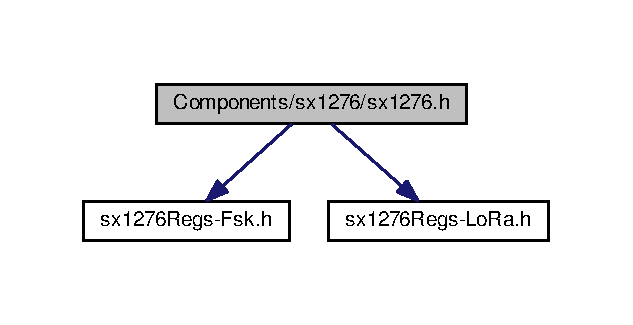
\includegraphics[width=304pt]{sx1276_8h__incl}
\end{center}
\end{figure}
This graph shows which files directly or indirectly include this file\+:
\nopagebreak
\begin{figure}[H]
\begin{center}
\leavevmode
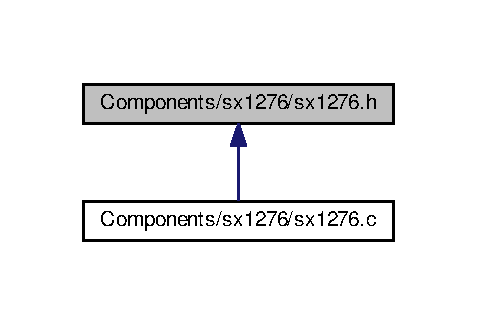
\includegraphics[width=229pt]{sx1276_8h__dep__incl}
\end{center}
\end{figure}
\subsection*{Data Structures}
\begin{DoxyCompactItemize}
\item 
struct \hyperlink{structRadioFskSettings__t}{Radio\+Fsk\+Settings\+\_\+t}
\item 
struct \hyperlink{structRadioFskPacketHandler__t}{Radio\+Fsk\+Packet\+Handler\+\_\+t}
\item 
struct \hyperlink{structRadioLoRaSettings__t}{Radio\+Lo\+Ra\+Settings\+\_\+t}
\item 
struct \hyperlink{structRadioLoRaPacketHandler__t}{Radio\+Lo\+Ra\+Packet\+Handler\+\_\+t}
\item 
struct \hyperlink{structRadioSettings__t}{Radio\+Settings\+\_\+t}
\item 
struct \hyperlink{structSX1276__s}{S\+X1276\+\_\+s}
\item 
struct \hyperlink{structsBoardCallback}{s\+Board\+Callback}
\end{DoxyCompactItemize}
\subsection*{Macros}
\begin{DoxyCompactItemize}
\item 
\#define \hyperlink{sx1276_8h_a42ef173c36527c948a507929f25f8e49}{R\+A\+D\+I\+O\+\_\+\+W\+A\+K\+E\+U\+P\+\_\+\+T\+I\+ME}~2
\item 
\#define \hyperlink{sx1276_8h_a51ad727a195c907dda006b5a40467136}{R\+F\+\_\+\+M\+I\+D\+\_\+\+B\+A\+N\+D\+\_\+\+T\+H\+R\+E\+SH}~525000000
\item 
\#define \hyperlink{sx1276_8h_a3a91534e6b1d9c4f1a179a495c38d7fe}{L\+O\+R\+A\+\_\+\+M\+A\+C\+\_\+\+P\+R\+I\+V\+A\+T\+E\+\_\+\+S\+Y\+N\+C\+W\+O\+RD}~0x12
\item 
\#define \hyperlink{sx1276_8h_ac2b07e04414b57bcebcb1eea5ba5ea70}{L\+O\+R\+A\+\_\+\+M\+A\+C\+\_\+\+P\+U\+B\+L\+I\+C\+\_\+\+S\+Y\+N\+C\+W\+O\+RD}~0x34
\item 
\#define \hyperlink{sx1276_8h_a3d24a8ac8f673b60ac35b6d92fe72747}{X\+T\+A\+L\+\_\+\+F\+R\+EQ}~32000000
\item 
\#define \hyperlink{sx1276_8h_ad7977f4d7c0acbc564d01fb225f94630}{F\+R\+E\+Q\+\_\+\+S\+T\+EP}~61.\+03515625
\item 
\#define \hyperlink{sx1276_8h_a0336ee1c2a498b2556d444cc28f32ba7}{F\+R\+E\+Q\+\_\+\+S\+T\+E\+P\+\_\+8}~15625 /$\ast$ \hyperlink{sx1276_8h_ad7977f4d7c0acbc564d01fb225f94630}{F\+R\+E\+Q\+\_\+\+S\+T\+EP}$<$$<$8 $\ast$/
\item 
\#define \hyperlink{sx1276_8h_abef7202d2ca987f0fe762a046d5cec52}{R\+A\+D\+I\+O\+\_\+\+I\+N\+I\+T\+\_\+\+R\+E\+G\+I\+S\+T\+E\+R\+S\+\_\+\+V\+A\+L\+UE}
\begin{DoxyCompactList}\small\item\em Radio hardware registers initialization definition. \end{DoxyCompactList}\item 
\#define \hyperlink{sx1276_8h_a398fcca28fef483bd7b9ea7345a805a0}{S\+X\+\_\+\+C\+H\+A\+N\+N\+E\+L\+\_\+\+T\+O\+\_\+\+F\+R\+EQ}(channel,  freq)
\item 
\#define \hyperlink{sx1276_8h_ab5f9f10543ab6e2b52e98b9ade9f1ada}{S\+X\+\_\+\+F\+R\+E\+Q\+\_\+\+T\+O\+\_\+\+C\+H\+A\+N\+N\+EL}(channel,  freq)
\item 
\#define \hyperlink{sx1276_8h_a739a2a1a0047c98ac1b18ecd25dac092}{R\+X\+\_\+\+B\+U\+F\+F\+E\+R\+\_\+\+S\+I\+ZE}~256
\end{DoxyCompactItemize}
\subsection*{Typedefs}
\begin{DoxyCompactItemize}
\item 
typedef struct \hyperlink{structSX1276__s}{S\+X1276\+\_\+s} \hyperlink{sx1276_8h_acf7f83d7d25c85897b88fcdc94345e56}{S\+X1276\+\_\+t}
\item 
typedef void() \hyperlink{sx1276_8h_af462584f307238535daaea42f6ce791c}{Dio\+Irq\+Handler}(void)
\item 
typedef struct \hyperlink{structsBoardCallback}{s\+Board\+Callback} \hyperlink{sx1276_8h_ad4ece8886feb1126f7cf786676572610}{Lo\+Ra\+Board\+Callback\+\_\+t}
\end{DoxyCompactItemize}
\subsection*{Functions}
\begin{DoxyCompactItemize}
\item 
void \hyperlink{sx1276_8h_afad8cc2a5afd223af9eba509bfaa15f4}{S\+X1276\+Board\+Init} (\hyperlink{sx1276_8h_ad4ece8886feb1126f7cf786676572610}{Lo\+Ra\+Board\+Callback\+\_\+t} $\ast$callbacks)
\item 
uint32\+\_\+t \hyperlink{sx1276_8h_a19a9ddff3f878b85e42c7571485fe3c8}{S\+X1276\+Init} (Radio\+Events\+\_\+t $\ast$events)
\begin{DoxyCompactList}\small\item\em Initializes the radio. \end{DoxyCompactList}\item 
void \hyperlink{sx1276_8h_aaaac2e0d7b5bd63fabf38a235d27a452}{S\+X1276\+Set\+Op\+Mode} (uint8\+\_\+t op\+Mode)
\begin{DoxyCompactList}\small\item\em Sets the S\+X1276 operating mode. \end{DoxyCompactList}\item 
Radio\+State\+\_\+t \hyperlink{sx1276_8h_ad70a0b1db3593630b1124653b6374944}{S\+X1276\+Get\+Status} (void)
\item 
void \hyperlink{sx1276_8h_a8325968bbefefab02537762dd274aa8b}{S\+X1276\+Set\+Modem} (Radio\+Modems\+\_\+t modem)
\begin{DoxyCompactList}\small\item\em Configures the radio with the given modem. \end{DoxyCompactList}\item 
void \hyperlink{sx1276_8h_a00768e908043081bc32cb83913192f7f}{S\+X1276\+Set\+Channel} (uint32\+\_\+t freq)
\begin{DoxyCompactList}\small\item\em Sets the channel configuration. \end{DoxyCompactList}\item 
bool \hyperlink{sx1276_8h_a29f26f7258f8fcd5c27800295639d7c7}{S\+X1276\+Is\+Channel\+Free} (Radio\+Modems\+\_\+t modem, uint32\+\_\+t freq, int16\+\_\+t rssi\+Thresh, uint32\+\_\+t max\+Carrier\+Sense\+Time)
\begin{DoxyCompactList}\small\item\em Checks if the channel is free for the given time. \end{DoxyCompactList}\item 
uint32\+\_\+t \hyperlink{sx1276_8h_a9ba39c96b8e339b06dd24543920fd2f7}{S\+X1276\+Random} (void)
\begin{DoxyCompactList}\small\item\em Generates a 32 bits random value based on the R\+S\+SI readings. \end{DoxyCompactList}\item 
void \hyperlink{sx1276_8h_a6a66ceb9e18a33aaff10d384fa493cf8}{S\+X1276\+Set\+Rx\+Config} (Radio\+Modems\+\_\+t modem, uint32\+\_\+t bandwidth, uint32\+\_\+t datarate, uint8\+\_\+t coderate, uint32\+\_\+t bandwidth\+Afc, uint16\+\_\+t preamble\+Len, uint16\+\_\+t symb\+Timeout, bool fix\+Len, uint8\+\_\+t payload\+Len, bool crc\+On, bool freq\+Hop\+On, uint8\+\_\+t hop\+Period, bool iq\+Inverted, bool rx\+Continuous)
\begin{DoxyCompactList}\small\item\em Sets the reception parameters. \end{DoxyCompactList}\item 
void \hyperlink{sx1276_8h_a805df2c0c4aa1630eeeb17177a600269}{S\+X1276\+Set\+Tx\+Config} (Radio\+Modems\+\_\+t modem, int8\+\_\+t power, uint32\+\_\+t fdev, uint32\+\_\+t bandwidth, uint32\+\_\+t datarate, uint8\+\_\+t coderate, uint16\+\_\+t preamble\+Len, bool fix\+Len, bool crc\+On, bool freq\+Hop\+On, uint8\+\_\+t hop\+Period, bool iq\+Inverted, uint32\+\_\+t timeout)
\begin{DoxyCompactList}\small\item\em Sets the transmission parameters. \end{DoxyCompactList}\item 
uint32\+\_\+t \hyperlink{sx1276_8h_a2d0bda0e5f9a4cce63284461e356b5e2}{S\+X1276\+Get\+Time\+On\+Air} (Radio\+Modems\+\_\+t modem, uint8\+\_\+t pkt\+Len)
\begin{DoxyCompactList}\small\item\em Computes the packet time on air in ms for the given payload. \end{DoxyCompactList}\item 
void \hyperlink{sx1276_8h_a901a3dcdbf26005e0f3f2def3e3d83b3}{S\+X1276\+Send} (uint8\+\_\+t $\ast$buffer, uint8\+\_\+t size)
\begin{DoxyCompactList}\small\item\em Sends the buffer of size. Prepares the packet to be sent and sets the radio in transmission. \end{DoxyCompactList}\item 
void \hyperlink{sx1276_8h_a32a7b8c477b2f400f96a3255e1ab7620}{S\+X1276\+Set\+Sleep} (void)
\begin{DoxyCompactList}\small\item\em Sets the radio in sleep mode. \end{DoxyCompactList}\item 
void \hyperlink{sx1276_8h_aaef7a98104b400b235ef76de0cfb17df}{S\+X1276\+Set\+Stby} (void)
\begin{DoxyCompactList}\small\item\em Sets the radio in standby mode. \end{DoxyCompactList}\item 
void \hyperlink{sx1276_8h_a8c2df9351fbde83379717dc6f76e5c11}{S\+X1276\+Set\+Rx} (uint32\+\_\+t timeout)
\begin{DoxyCompactList}\small\item\em Sets the radio in reception mode for the given time. \end{DoxyCompactList}\item 
void \hyperlink{sx1276_8h_a9958c574c62b2235c4f3d4d6571854db}{S\+X1276\+Start\+Cad} (void)
\begin{DoxyCompactList}\small\item\em Start a Channel Activity Detection. \end{DoxyCompactList}\item 
void \hyperlink{sx1276_8h_ac77895b054eb64df0ee2fa97061efae8}{S\+X1276\+Set\+Tx\+Continuous\+Wave} (uint32\+\_\+t freq, int8\+\_\+t power, uint16\+\_\+t time)
\begin{DoxyCompactList}\small\item\em Sets the radio in continuous wave transmission mode. \end{DoxyCompactList}\item 
int16\+\_\+t \hyperlink{sx1276_8h_a5741300714435f1dd69084a30031f6e3}{S\+X1276\+Read\+Rssi} (Radio\+Modems\+\_\+t modem)
\begin{DoxyCompactList}\small\item\em Reads the current R\+S\+SI value. \end{DoxyCompactList}\item 
void \hyperlink{sx1276_8h_a77f5d37bad59c99a14637f1eee273edc}{S\+X1276\+Write} (uint8\+\_\+t addr, uint8\+\_\+t data)
\begin{DoxyCompactList}\small\item\em Writes the radio register at the specified address. \end{DoxyCompactList}\item 
uint8\+\_\+t \hyperlink{sx1276_8h_a80f15707dfe79d5cd46a9e3d78214522}{S\+X1276\+Read} (uint8\+\_\+t addr)
\begin{DoxyCompactList}\small\item\em Reads the radio register at the specified address. \end{DoxyCompactList}\item 
void \hyperlink{sx1276_8h_a9fbc81d0d84656f61feca7ce78dda70b}{S\+X1276\+Write\+Buffer} (uint8\+\_\+t addr, uint8\+\_\+t $\ast$buffer, uint8\+\_\+t size)
\begin{DoxyCompactList}\small\item\em Writes multiple radio registers starting at address. \end{DoxyCompactList}\item 
void \hyperlink{sx1276_8h_a26a0fc71f16d6bd65124e21b7045e0aa}{S\+X1276\+Read\+Buffer} (uint8\+\_\+t addr, uint8\+\_\+t $\ast$buffer, uint8\+\_\+t size)
\begin{DoxyCompactList}\small\item\em Reads multiple radio registers starting at address. \end{DoxyCompactList}\item 
void \hyperlink{sx1276_8h_aac0bb6d289a1afe69f550cb148f3bac8}{S\+X1276\+Set\+Max\+Payload\+Length} (Radio\+Modems\+\_\+t modem, uint8\+\_\+t max)
\begin{DoxyCompactList}\small\item\em Sets the maximum payload length. \end{DoxyCompactList}\item 
void \hyperlink{sx1276_8h_a8acacaf2d3e05a712a90f587d1908c6c}{S\+X1276\+Set\+Public\+Network} (bool enable)
\begin{DoxyCompactList}\small\item\em Sets the network to public or private. Updates the sync byte. \end{DoxyCompactList}\item 
uint32\+\_\+t \hyperlink{sx1276_8h_a9b6e3fa7bd90fa2dce95ef4d00db7bfe}{S\+X1276\+Get\+Radio\+Wake\+Up\+Time} (void)
\begin{DoxyCompactList}\small\item\em Service to get the radio wake-\/up time. \end{DoxyCompactList}\end{DoxyCompactItemize}
\subsection*{Variables}
\begin{DoxyCompactItemize}
\item 
\hyperlink{sx1276_8h_acf7f83d7d25c85897b88fcdc94345e56}{S\+X1276\+\_\+t} \hyperlink{sx1276_8h_a91a81a798b3d849e2cc114c18bf9c5cc}{S\+X1276}
\end{DoxyCompactItemize}


\subsection{Macro Definition Documentation}
\mbox{\Hypertarget{sx1276_8h_ad7977f4d7c0acbc564d01fb225f94630}\label{sx1276_8h_ad7977f4d7c0acbc564d01fb225f94630}} 
\index{sx1276.\+h@{sx1276.\+h}!F\+R\+E\+Q\+\_\+\+S\+T\+EP@{F\+R\+E\+Q\+\_\+\+S\+T\+EP}}
\index{F\+R\+E\+Q\+\_\+\+S\+T\+EP@{F\+R\+E\+Q\+\_\+\+S\+T\+EP}!sx1276.\+h@{sx1276.\+h}}
\subsubsection{\texorpdfstring{F\+R\+E\+Q\+\_\+\+S\+T\+EP}{FREQ\_STEP}}
{\footnotesize\ttfamily \#define F\+R\+E\+Q\+\_\+\+S\+T\+EP~61.\+03515625}

\mbox{\Hypertarget{sx1276_8h_a0336ee1c2a498b2556d444cc28f32ba7}\label{sx1276_8h_a0336ee1c2a498b2556d444cc28f32ba7}} 
\index{sx1276.\+h@{sx1276.\+h}!F\+R\+E\+Q\+\_\+\+S\+T\+E\+P\+\_\+8@{F\+R\+E\+Q\+\_\+\+S\+T\+E\+P\+\_\+8}}
\index{F\+R\+E\+Q\+\_\+\+S\+T\+E\+P\+\_\+8@{F\+R\+E\+Q\+\_\+\+S\+T\+E\+P\+\_\+8}!sx1276.\+h@{sx1276.\+h}}
\subsubsection{\texorpdfstring{F\+R\+E\+Q\+\_\+\+S\+T\+E\+P\+\_\+8}{FREQ\_STEP\_8}}
{\footnotesize\ttfamily \#define F\+R\+E\+Q\+\_\+\+S\+T\+E\+P\+\_\+8~15625 /$\ast$ \hyperlink{sx1276_8h_ad7977f4d7c0acbc564d01fb225f94630}{F\+R\+E\+Q\+\_\+\+S\+T\+EP}$<$$<$8 $\ast$/}

\mbox{\Hypertarget{sx1276_8h_a3a91534e6b1d9c4f1a179a495c38d7fe}\label{sx1276_8h_a3a91534e6b1d9c4f1a179a495c38d7fe}} 
\index{sx1276.\+h@{sx1276.\+h}!L\+O\+R\+A\+\_\+\+M\+A\+C\+\_\+\+P\+R\+I\+V\+A\+T\+E\+\_\+\+S\+Y\+N\+C\+W\+O\+RD@{L\+O\+R\+A\+\_\+\+M\+A\+C\+\_\+\+P\+R\+I\+V\+A\+T\+E\+\_\+\+S\+Y\+N\+C\+W\+O\+RD}}
\index{L\+O\+R\+A\+\_\+\+M\+A\+C\+\_\+\+P\+R\+I\+V\+A\+T\+E\+\_\+\+S\+Y\+N\+C\+W\+O\+RD@{L\+O\+R\+A\+\_\+\+M\+A\+C\+\_\+\+P\+R\+I\+V\+A\+T\+E\+\_\+\+S\+Y\+N\+C\+W\+O\+RD}!sx1276.\+h@{sx1276.\+h}}
\subsubsection{\texorpdfstring{L\+O\+R\+A\+\_\+\+M\+A\+C\+\_\+\+P\+R\+I\+V\+A\+T\+E\+\_\+\+S\+Y\+N\+C\+W\+O\+RD}{LORA\_MAC\_PRIVATE\_SYNCWORD}}
{\footnotesize\ttfamily \#define L\+O\+R\+A\+\_\+\+M\+A\+C\+\_\+\+P\+R\+I\+V\+A\+T\+E\+\_\+\+S\+Y\+N\+C\+W\+O\+RD~0x12}

Sync word for Private Lo\+Ra networks \mbox{\Hypertarget{sx1276_8h_ac2b07e04414b57bcebcb1eea5ba5ea70}\label{sx1276_8h_ac2b07e04414b57bcebcb1eea5ba5ea70}} 
\index{sx1276.\+h@{sx1276.\+h}!L\+O\+R\+A\+\_\+\+M\+A\+C\+\_\+\+P\+U\+B\+L\+I\+C\+\_\+\+S\+Y\+N\+C\+W\+O\+RD@{L\+O\+R\+A\+\_\+\+M\+A\+C\+\_\+\+P\+U\+B\+L\+I\+C\+\_\+\+S\+Y\+N\+C\+W\+O\+RD}}
\index{L\+O\+R\+A\+\_\+\+M\+A\+C\+\_\+\+P\+U\+B\+L\+I\+C\+\_\+\+S\+Y\+N\+C\+W\+O\+RD@{L\+O\+R\+A\+\_\+\+M\+A\+C\+\_\+\+P\+U\+B\+L\+I\+C\+\_\+\+S\+Y\+N\+C\+W\+O\+RD}!sx1276.\+h@{sx1276.\+h}}
\subsubsection{\texorpdfstring{L\+O\+R\+A\+\_\+\+M\+A\+C\+\_\+\+P\+U\+B\+L\+I\+C\+\_\+\+S\+Y\+N\+C\+W\+O\+RD}{LORA\_MAC\_PUBLIC\_SYNCWORD}}
{\footnotesize\ttfamily \#define L\+O\+R\+A\+\_\+\+M\+A\+C\+\_\+\+P\+U\+B\+L\+I\+C\+\_\+\+S\+Y\+N\+C\+W\+O\+RD~0x34}

Sync word for Public Lo\+Ra networks \mbox{\Hypertarget{sx1276_8h_abef7202d2ca987f0fe762a046d5cec52}\label{sx1276_8h_abef7202d2ca987f0fe762a046d5cec52}} 
\index{sx1276.\+h@{sx1276.\+h}!R\+A\+D\+I\+O\+\_\+\+I\+N\+I\+T\+\_\+\+R\+E\+G\+I\+S\+T\+E\+R\+S\+\_\+\+V\+A\+L\+UE@{R\+A\+D\+I\+O\+\_\+\+I\+N\+I\+T\+\_\+\+R\+E\+G\+I\+S\+T\+E\+R\+S\+\_\+\+V\+A\+L\+UE}}
\index{R\+A\+D\+I\+O\+\_\+\+I\+N\+I\+T\+\_\+\+R\+E\+G\+I\+S\+T\+E\+R\+S\+\_\+\+V\+A\+L\+UE@{R\+A\+D\+I\+O\+\_\+\+I\+N\+I\+T\+\_\+\+R\+E\+G\+I\+S\+T\+E\+R\+S\+\_\+\+V\+A\+L\+UE}!sx1276.\+h@{sx1276.\+h}}
\subsubsection{\texorpdfstring{R\+A\+D\+I\+O\+\_\+\+I\+N\+I\+T\+\_\+\+R\+E\+G\+I\+S\+T\+E\+R\+S\+\_\+\+V\+A\+L\+UE}{RADIO\_INIT\_REGISTERS\_VALUE}}
{\footnotesize\ttfamily \#define R\+A\+D\+I\+O\+\_\+\+I\+N\+I\+T\+\_\+\+R\+E\+G\+I\+S\+T\+E\+R\+S\+\_\+\+V\+A\+L\+UE}

{\bfseries Value\+:}
\begin{DoxyCode}
\{                                                 \(\backslash\)
    \{ MODEM\_FSK , \hyperlink{sx1276Regs-Fsk_8h_ab08aa4c56ad75b3e715a1115330109ca}{REG\_LNA}                , 0x23 \},\(\backslash\)
    \{ MODEM\_FSK , \hyperlink{sx1276Regs-Fsk_8h_a6bba52e363d49d2783439eb8062d90c8}{REG\_RXCONFIG}           , 0x1E \},\(\backslash\)
    \{ MODEM\_FSK , \hyperlink{sx1276Regs-Fsk_8h_a9ba1a67481c3ba0a454cb4873e4db10b}{REG\_RSSICONFIG}         , 0xD2 \},\(\backslash\)
    \{ MODEM\_FSK , \hyperlink{sx1276Regs-Fsk_8h_a04f60f1d03035cf80cebff9648a894c0}{REG\_AFCFEI}             , 0x01 \},\(\backslash\)
    \{ MODEM\_FSK , \hyperlink{sx1276Regs-Fsk_8h_a8acf717d67c4e7f4b92a25653ddb495c}{REG\_PREAMBLEDETECT}     , 0xAA \},\(\backslash\)
    \{ MODEM\_FSK , \hyperlink{sx1276Regs-Fsk_8h_a1edb093ed684495473ecd2e97e3a49c2}{REG\_OSC}                , 0x07 \},\(\backslash\)
    \{ MODEM\_FSK , \hyperlink{sx1276Regs-Fsk_8h_ae80bd3142a5c405bf7063ac7b0e8e101}{REG\_SYNCCONFIG}         , 0x12 \},\(\backslash\)
    \{ MODEM\_FSK , \hyperlink{sx1276Regs-Fsk_8h_a4d0160e654656b6cd6426c295c8e131b}{REG\_SYNCVALUE1}         , 0xC1 \},\(\backslash\)
    \{ MODEM\_FSK , \hyperlink{sx1276Regs-Fsk_8h_a840d780f6d455dc828e2ec8217e9043a}{REG\_SYNCVALUE2}         , 0x94 \},\(\backslash\)
    \{ MODEM\_FSK , \hyperlink{sx1276Regs-Fsk_8h_af89062529e96d32eecd0f89963d52adf}{REG\_SYNCVALUE3}         , 0xC1 \},\(\backslash\)
    \{ MODEM\_FSK , \hyperlink{sx1276Regs-Fsk_8h_a035c91c3eea7209c78ac5bda775940cc}{REG\_PACKETCONFIG1}      , 0xD8 \},\(\backslash\)
    \{ MODEM\_FSK , \hyperlink{sx1276Regs-Fsk_8h_a18b41b1ddfbe6eb514f74431b5d76792}{REG\_FIFOTHRESH}         , 0x8F \},\(\backslash\)
    \{ MODEM\_FSK , \hyperlink{sx1276Regs-Fsk_8h_aeb557bae3e3e5ffb390a6f6a61ac686d}{REG\_IMAGECAL}           , 0x02 \},\(\backslash\)
    \{ MODEM\_FSK , \hyperlink{sx1276Regs-Fsk_8h_ac16d5678e98fa6ab73655240a11f9b69}{REG\_DIOMAPPING1}        , 0x00 \},\(\backslash\)
    \{ MODEM\_FSK , \hyperlink{sx1276Regs-Fsk_8h_aec8b1ddf72925f502675593fabcc469f}{REG\_DIOMAPPING2}        , 0x30 \},\(\backslash\)
    \{ MODEM\_LORA, \hyperlink{sx1276Regs-LoRa_8h_ae71e7acfa7c8c737e55349e72c71349f}{REG\_LR\_PAYLOADMAXLENGTH}, 0x40 \},\(\backslash\)
\}                                                 \(\backslash\)
\end{DoxyCode}


Radio hardware registers initialization definition. 

\begin{DoxyRemark}{Remarks}
Can be automatically generated by the S\+X1276 G\+UI (not yet implemented) 
\end{DoxyRemark}
\mbox{\Hypertarget{sx1276_8h_a42ef173c36527c948a507929f25f8e49}\label{sx1276_8h_a42ef173c36527c948a507929f25f8e49}} 
\index{sx1276.\+h@{sx1276.\+h}!R\+A\+D\+I\+O\+\_\+\+W\+A\+K\+E\+U\+P\+\_\+\+T\+I\+ME@{R\+A\+D\+I\+O\+\_\+\+W\+A\+K\+E\+U\+P\+\_\+\+T\+I\+ME}}
\index{R\+A\+D\+I\+O\+\_\+\+W\+A\+K\+E\+U\+P\+\_\+\+T\+I\+ME@{R\+A\+D\+I\+O\+\_\+\+W\+A\+K\+E\+U\+P\+\_\+\+T\+I\+ME}!sx1276.\+h@{sx1276.\+h}}
\subsubsection{\texorpdfstring{R\+A\+D\+I\+O\+\_\+\+W\+A\+K\+E\+U\+P\+\_\+\+T\+I\+ME}{RADIO\_WAKEUP\_TIME}}
{\footnotesize\ttfamily \#define R\+A\+D\+I\+O\+\_\+\+W\+A\+K\+E\+U\+P\+\_\+\+T\+I\+ME~2}

Radio wake-\/up time from sleep \mbox{\Hypertarget{sx1276_8h_a51ad727a195c907dda006b5a40467136}\label{sx1276_8h_a51ad727a195c907dda006b5a40467136}} 
\index{sx1276.\+h@{sx1276.\+h}!R\+F\+\_\+\+M\+I\+D\+\_\+\+B\+A\+N\+D\+\_\+\+T\+H\+R\+E\+SH@{R\+F\+\_\+\+M\+I\+D\+\_\+\+B\+A\+N\+D\+\_\+\+T\+H\+R\+E\+SH}}
\index{R\+F\+\_\+\+M\+I\+D\+\_\+\+B\+A\+N\+D\+\_\+\+T\+H\+R\+E\+SH@{R\+F\+\_\+\+M\+I\+D\+\_\+\+B\+A\+N\+D\+\_\+\+T\+H\+R\+E\+SH}!sx1276.\+h@{sx1276.\+h}}
\subsubsection{\texorpdfstring{R\+F\+\_\+\+M\+I\+D\+\_\+\+B\+A\+N\+D\+\_\+\+T\+H\+R\+E\+SH}{RF\_MID\_BAND\_THRESH}}
{\footnotesize\ttfamily \#define R\+F\+\_\+\+M\+I\+D\+\_\+\+B\+A\+N\+D\+\_\+\+T\+H\+R\+E\+SH~525000000}

\mbox{\Hypertarget{sx1276_8h_a739a2a1a0047c98ac1b18ecd25dac092}\label{sx1276_8h_a739a2a1a0047c98ac1b18ecd25dac092}} 
\index{sx1276.\+h@{sx1276.\+h}!R\+X\+\_\+\+B\+U\+F\+F\+E\+R\+\_\+\+S\+I\+ZE@{R\+X\+\_\+\+B\+U\+F\+F\+E\+R\+\_\+\+S\+I\+ZE}}
\index{R\+X\+\_\+\+B\+U\+F\+F\+E\+R\+\_\+\+S\+I\+ZE@{R\+X\+\_\+\+B\+U\+F\+F\+E\+R\+\_\+\+S\+I\+ZE}!sx1276.\+h@{sx1276.\+h}}
\subsubsection{\texorpdfstring{R\+X\+\_\+\+B\+U\+F\+F\+E\+R\+\_\+\+S\+I\+ZE}{RX\_BUFFER\_SIZE}}
{\footnotesize\ttfamily \#define R\+X\+\_\+\+B\+U\+F\+F\+E\+R\+\_\+\+S\+I\+ZE~256}

\mbox{\Hypertarget{sx1276_8h_a398fcca28fef483bd7b9ea7345a805a0}\label{sx1276_8h_a398fcca28fef483bd7b9ea7345a805a0}} 
\index{sx1276.\+h@{sx1276.\+h}!S\+X\+\_\+\+C\+H\+A\+N\+N\+E\+L\+\_\+\+T\+O\+\_\+\+F\+R\+EQ@{S\+X\+\_\+\+C\+H\+A\+N\+N\+E\+L\+\_\+\+T\+O\+\_\+\+F\+R\+EQ}}
\index{S\+X\+\_\+\+C\+H\+A\+N\+N\+E\+L\+\_\+\+T\+O\+\_\+\+F\+R\+EQ@{S\+X\+\_\+\+C\+H\+A\+N\+N\+E\+L\+\_\+\+T\+O\+\_\+\+F\+R\+EQ}!sx1276.\+h@{sx1276.\+h}}
\subsubsection{\texorpdfstring{S\+X\+\_\+\+C\+H\+A\+N\+N\+E\+L\+\_\+\+T\+O\+\_\+\+F\+R\+EQ}{SX\_CHANNEL\_TO\_FREQ}}
{\footnotesize\ttfamily \#define S\+X\+\_\+\+C\+H\+A\+N\+N\+E\+L\+\_\+\+T\+O\+\_\+\+F\+R\+EQ(\begin{DoxyParamCaption}\item[{}]{channel,  }\item[{}]{freq }\end{DoxyParamCaption})}

{\bfseries Value\+:}
\begin{DoxyCode}
\textcolor{keywordflow}{do}                                                                                              \(\backslash\)
    \{                                                                                               \(\backslash\)
        uint32\_t initialChanInt, initialChanFrac;                                                   \(\backslash\)
        initialChanInt = channel  >> 8;                                                             \(\backslash\)
        initialChanFrac = channel - ( initialChanInt << 8 );                                        \(\backslash\)
        freq = initialChanInt * \hyperlink{sx1276_8h_a0336ee1c2a498b2556d444cc28f32ba7}{FREQ\_STEP\_8} + ( ( initialChanFrac * 
      \hyperlink{sx1276_8h_a0336ee1c2a498b2556d444cc28f32ba7}{FREQ\_STEP\_8} + ( 128 ) ) >> 8 ); \(\backslash\)
    \}\textcolor{keywordflow}{while}( 0 )
\end{DoxyCode}
\mbox{\Hypertarget{sx1276_8h_ab5f9f10543ab6e2b52e98b9ade9f1ada}\label{sx1276_8h_ab5f9f10543ab6e2b52e98b9ade9f1ada}} 
\index{sx1276.\+h@{sx1276.\+h}!S\+X\+\_\+\+F\+R\+E\+Q\+\_\+\+T\+O\+\_\+\+C\+H\+A\+N\+N\+EL@{S\+X\+\_\+\+F\+R\+E\+Q\+\_\+\+T\+O\+\_\+\+C\+H\+A\+N\+N\+EL}}
\index{S\+X\+\_\+\+F\+R\+E\+Q\+\_\+\+T\+O\+\_\+\+C\+H\+A\+N\+N\+EL@{S\+X\+\_\+\+F\+R\+E\+Q\+\_\+\+T\+O\+\_\+\+C\+H\+A\+N\+N\+EL}!sx1276.\+h@{sx1276.\+h}}
\subsubsection{\texorpdfstring{S\+X\+\_\+\+F\+R\+E\+Q\+\_\+\+T\+O\+\_\+\+C\+H\+A\+N\+N\+EL}{SX\_FREQ\_TO\_CHANNEL}}
{\footnotesize\ttfamily \#define S\+X\+\_\+\+F\+R\+E\+Q\+\_\+\+T\+O\+\_\+\+C\+H\+A\+N\+N\+EL(\begin{DoxyParamCaption}\item[{}]{channel,  }\item[{}]{freq }\end{DoxyParamCaption})}

{\bfseries Value\+:}
\begin{DoxyCode}
\textcolor{keywordflow}{do}                                                                                                         
         \(\backslash\)
    \{                                                                                                      
             \(\backslash\)
        uint32\_t initialFreqInt, initialFreqFrac;                                                          
             \(\backslash\)
        initialFreqInt = freq / \hyperlink{sx1276_8h_a0336ee1c2a498b2556d444cc28f32ba7}{FREQ\_STEP\_8};                                                    
                        \(\backslash\)
        initialFreqFrac = freq - ( initialFreqInt * \hyperlink{sx1276_8h_a0336ee1c2a498b2556d444cc28f32ba7}{FREQ\_STEP\_8} );                              
                        \(\backslash\)
        channel = ( initialFreqInt << 8 ) + ( ( ( initialFreqFrac << 8 ) + ( 
      \hyperlink{sx1276_8h_a0336ee1c2a498b2556d444cc28f32ba7}{FREQ\_STEP\_8} / 2 ) ) / \hyperlink{sx1276_8h_a0336ee1c2a498b2556d444cc28f32ba7}{FREQ\_STEP\_8} ); \(\backslash\)
    \}\textcolor{keywordflow}{while}( 0 )
\end{DoxyCode}
\mbox{\Hypertarget{sx1276_8h_a3d24a8ac8f673b60ac35b6d92fe72747}\label{sx1276_8h_a3d24a8ac8f673b60ac35b6d92fe72747}} 
\index{sx1276.\+h@{sx1276.\+h}!X\+T\+A\+L\+\_\+\+F\+R\+EQ@{X\+T\+A\+L\+\_\+\+F\+R\+EQ}}
\index{X\+T\+A\+L\+\_\+\+F\+R\+EQ@{X\+T\+A\+L\+\_\+\+F\+R\+EQ}!sx1276.\+h@{sx1276.\+h}}
\subsubsection{\texorpdfstring{X\+T\+A\+L\+\_\+\+F\+R\+EQ}{XTAL\_FREQ}}
{\footnotesize\ttfamily \#define X\+T\+A\+L\+\_\+\+F\+R\+EQ~32000000}

S\+X1276 definitions 

\subsection{Typedef Documentation}
\mbox{\Hypertarget{sx1276_8h_af462584f307238535daaea42f6ce791c}\label{sx1276_8h_af462584f307238535daaea42f6ce791c}} 
\index{sx1276.\+h@{sx1276.\+h}!Dio\+Irq\+Handler@{Dio\+Irq\+Handler}}
\index{Dio\+Irq\+Handler@{Dio\+Irq\+Handler}!sx1276.\+h@{sx1276.\+h}}
\subsubsection{\texorpdfstring{Dio\+Irq\+Handler}{DioIrqHandler}}
{\footnotesize\ttfamily typedef void() Dio\+Irq\+Handler(void)}

Hardware IO I\+RQ callback function definition \mbox{\Hypertarget{sx1276_8h_ad4ece8886feb1126f7cf786676572610}\label{sx1276_8h_ad4ece8886feb1126f7cf786676572610}} 
\index{sx1276.\+h@{sx1276.\+h}!Lo\+Ra\+Board\+Callback\+\_\+t@{Lo\+Ra\+Board\+Callback\+\_\+t}}
\index{Lo\+Ra\+Board\+Callback\+\_\+t@{Lo\+Ra\+Board\+Callback\+\_\+t}!sx1276.\+h@{sx1276.\+h}}
\subsubsection{\texorpdfstring{Lo\+Ra\+Board\+Callback\+\_\+t}{LoRaBoardCallback\_t}}
{\footnotesize\ttfamily typedef struct \hyperlink{structsBoardCallback}{s\+Board\+Callback} \hyperlink{sx1276_8h_ad4ece8886feb1126f7cf786676572610}{Lo\+Ra\+Board\+Callback\+\_\+t}}

\mbox{\Hypertarget{sx1276_8h_acf7f83d7d25c85897b88fcdc94345e56}\label{sx1276_8h_acf7f83d7d25c85897b88fcdc94345e56}} 
\index{sx1276.\+h@{sx1276.\+h}!S\+X1276\+\_\+t@{S\+X1276\+\_\+t}}
\index{S\+X1276\+\_\+t@{S\+X1276\+\_\+t}!sx1276.\+h@{sx1276.\+h}}
\subsubsection{\texorpdfstring{S\+X1276\+\_\+t}{SX1276\_t}}
{\footnotesize\ttfamily typedef struct \hyperlink{structSX1276__s}{S\+X1276\+\_\+s} \hyperlink{sx1276_8h_acf7f83d7d25c85897b88fcdc94345e56}{S\+X1276\+\_\+t}}

Radio hardware and global parameters 

\subsection{Function Documentation}
\mbox{\Hypertarget{sx1276_8h_afad8cc2a5afd223af9eba509bfaa15f4}\label{sx1276_8h_afad8cc2a5afd223af9eba509bfaa15f4}} 
\index{sx1276.\+h@{sx1276.\+h}!S\+X1276\+Board\+Init@{S\+X1276\+Board\+Init}}
\index{S\+X1276\+Board\+Init@{S\+X1276\+Board\+Init}!sx1276.\+h@{sx1276.\+h}}
\subsubsection{\texorpdfstring{S\+X1276\+Board\+Init()}{SX1276BoardInit()}}
{\footnotesize\ttfamily void S\+X1276\+Board\+Init (\begin{DoxyParamCaption}\item[{\hyperlink{sx1276_8h_ad4ece8886feb1126f7cf786676572610}{Lo\+Ra\+Board\+Callback\+\_\+t} $\ast$}]{callbacks }\end{DoxyParamCaption})}

============================================================================ \subsection*{Public functions prototypes }\mbox{\Hypertarget{sx1276_8h_a9b6e3fa7bd90fa2dce95ef4d00db7bfe}\label{sx1276_8h_a9b6e3fa7bd90fa2dce95ef4d00db7bfe}} 
\index{sx1276.\+h@{sx1276.\+h}!S\+X1276\+Get\+Radio\+Wake\+Up\+Time@{S\+X1276\+Get\+Radio\+Wake\+Up\+Time}}
\index{S\+X1276\+Get\+Radio\+Wake\+Up\+Time@{S\+X1276\+Get\+Radio\+Wake\+Up\+Time}!sx1276.\+h@{sx1276.\+h}}
\subsubsection{\texorpdfstring{S\+X1276\+Get\+Radio\+Wake\+Up\+Time()}{SX1276GetRadioWakeUpTime()}}
{\footnotesize\ttfamily uint32\+\_\+t S\+X1276\+Get\+Radio\+Wake\+Up\+Time (\begin{DoxyParamCaption}\item[{void}]{ }\end{DoxyParamCaption})}



Service to get the radio wake-\/up time. 


\begin{DoxyRetVals}{Return values}
{\em Value} & of the radio wake-\/up time. \\
\hline
\end{DoxyRetVals}
\mbox{\Hypertarget{sx1276_8h_ad70a0b1db3593630b1124653b6374944}\label{sx1276_8h_ad70a0b1db3593630b1124653b6374944}} 
\index{sx1276.\+h@{sx1276.\+h}!S\+X1276\+Get\+Status@{S\+X1276\+Get\+Status}}
\index{S\+X1276\+Get\+Status@{S\+X1276\+Get\+Status}!sx1276.\+h@{sx1276.\+h}}
\subsubsection{\texorpdfstring{S\+X1276\+Get\+Status()}{SX1276GetStatus()}}
{\footnotesize\ttfamily Radio\+State\+\_\+t S\+X1276\+Get\+Status (\begin{DoxyParamCaption}\item[{void}]{ }\end{DoxyParamCaption})}

Return current radio status


\begin{DoxyParams}{Parameters}
{\em status} & Radio status.\mbox{[}R\+F\+\_\+\+I\+D\+LE, R\+F\+\_\+\+R\+X\+\_\+\+R\+U\+N\+N\+I\+NG, R\+F\+\_\+\+T\+X\+\_\+\+R\+U\+N\+N\+I\+NG\mbox{]} \\
\hline
\end{DoxyParams}
\mbox{\Hypertarget{sx1276_8h_a2d0bda0e5f9a4cce63284461e356b5e2}\label{sx1276_8h_a2d0bda0e5f9a4cce63284461e356b5e2}} 
\index{sx1276.\+h@{sx1276.\+h}!S\+X1276\+Get\+Time\+On\+Air@{S\+X1276\+Get\+Time\+On\+Air}}
\index{S\+X1276\+Get\+Time\+On\+Air@{S\+X1276\+Get\+Time\+On\+Air}!sx1276.\+h@{sx1276.\+h}}
\subsubsection{\texorpdfstring{S\+X1276\+Get\+Time\+On\+Air()}{SX1276GetTimeOnAir()}}
{\footnotesize\ttfamily uint32\+\_\+t S\+X1276\+Get\+Time\+On\+Air (\begin{DoxyParamCaption}\item[{Radio\+Modems\+\_\+t}]{modem,  }\item[{uint8\+\_\+t}]{pkt\+Len }\end{DoxyParamCaption})}



Computes the packet time on air in ms for the given payload. 

Can only be called once Set\+Rx\+Config or Set\+Tx\+Config have been called


\begin{DoxyParams}{Parameters}
{\em \mbox{[}\+I\+N\mbox{]}} & modem Radio modem to be used \mbox{[}0\+: F\+SK, 1\+: Lo\+Ra\mbox{]} \\
\hline
{\em \mbox{[}\+I\+N\mbox{]}} & pkt\+Len Packet payload length\\
\hline
\end{DoxyParams}

\begin{DoxyRetVals}{Return values}
{\em air\+Time} & Computed air\+Time (ms) for the given packet payload length \\
\hline
\end{DoxyRetVals}
\mbox{\Hypertarget{sx1276_8h_a19a9ddff3f878b85e42c7571485fe3c8}\label{sx1276_8h_a19a9ddff3f878b85e42c7571485fe3c8}} 
\index{sx1276.\+h@{sx1276.\+h}!S\+X1276\+Init@{S\+X1276\+Init}}
\index{S\+X1276\+Init@{S\+X1276\+Init}!sx1276.\+h@{sx1276.\+h}}
\subsubsection{\texorpdfstring{S\+X1276\+Init()}{SX1276Init()}}
{\footnotesize\ttfamily uint32\+\_\+t S\+X1276\+Init (\begin{DoxyParamCaption}\item[{Radio\+Events\+\_\+t $\ast$}]{events }\end{DoxyParamCaption})}



Initializes the radio. 


\begin{DoxyParams}{Parameters}
{\em \mbox{[}\+I\+N\mbox{]}} & events Structure containing the driver callback functions \\
\hline
{\em \mbox{[}\+O\+U\+T\mbox{]}} & returns the wake up time of the radio and associated board \\
\hline
\end{DoxyParams}
\mbox{\Hypertarget{sx1276_8h_a29f26f7258f8fcd5c27800295639d7c7}\label{sx1276_8h_a29f26f7258f8fcd5c27800295639d7c7}} 
\index{sx1276.\+h@{sx1276.\+h}!S\+X1276\+Is\+Channel\+Free@{S\+X1276\+Is\+Channel\+Free}}
\index{S\+X1276\+Is\+Channel\+Free@{S\+X1276\+Is\+Channel\+Free}!sx1276.\+h@{sx1276.\+h}}
\subsubsection{\texorpdfstring{S\+X1276\+Is\+Channel\+Free()}{SX1276IsChannelFree()}}
{\footnotesize\ttfamily bool S\+X1276\+Is\+Channel\+Free (\begin{DoxyParamCaption}\item[{Radio\+Modems\+\_\+t}]{modem,  }\item[{uint32\+\_\+t}]{freq,  }\item[{int16\+\_\+t}]{rssi\+Thresh,  }\item[{uint32\+\_\+t}]{max\+Carrier\+Sense\+Time }\end{DoxyParamCaption})}



Checks if the channel is free for the given time. 


\begin{DoxyParams}{Parameters}
{\em \mbox{[}\+I\+N\mbox{]}} & modem Radio modem to be used \mbox{[}0\+: F\+SK, 1\+: Lo\+Ra\mbox{]} \\
\hline
{\em \mbox{[}\+I\+N\mbox{]}} & freq Channel RF frequency \\
\hline
{\em \mbox{[}\+I\+N\mbox{]}} & rssi\+Thresh R\+S\+SI threshold \\
\hline
{\em \mbox{[}\+I\+N\mbox{]}} & max\+Carrier\+Sense\+Time Max time while the R\+S\+SI is measured\\
\hline
\end{DoxyParams}

\begin{DoxyRetVals}{Return values}
{\em is\+Free} & \mbox{[}true\+: Channel is free, false\+: Channel is not free\mbox{]} \\
\hline
\end{DoxyRetVals}
\mbox{\Hypertarget{sx1276_8h_a9ba39c96b8e339b06dd24543920fd2f7}\label{sx1276_8h_a9ba39c96b8e339b06dd24543920fd2f7}} 
\index{sx1276.\+h@{sx1276.\+h}!S\+X1276\+Random@{S\+X1276\+Random}}
\index{S\+X1276\+Random@{S\+X1276\+Random}!sx1276.\+h@{sx1276.\+h}}
\subsubsection{\texorpdfstring{S\+X1276\+Random()}{SX1276Random()}}
{\footnotesize\ttfamily uint32\+\_\+t S\+X1276\+Random (\begin{DoxyParamCaption}\item[{void}]{ }\end{DoxyParamCaption})}



Generates a 32 bits random value based on the R\+S\+SI readings. 

\begin{DoxyRemark}{Remarks}
This function sets the radio in Lo\+Ra modem mode and disables all interrupts. After calling this function either S\+X1276\+Set\+Rx\+Config or S\+X1276\+Set\+Tx\+Config functions must be called.
\end{DoxyRemark}

\begin{DoxyRetVals}{Return values}
{\em random\+Value} & 32 bits random value \\
\hline
\end{DoxyRetVals}
\mbox{\Hypertarget{sx1276_8h_a80f15707dfe79d5cd46a9e3d78214522}\label{sx1276_8h_a80f15707dfe79d5cd46a9e3d78214522}} 
\index{sx1276.\+h@{sx1276.\+h}!S\+X1276\+Read@{S\+X1276\+Read}}
\index{S\+X1276\+Read@{S\+X1276\+Read}!sx1276.\+h@{sx1276.\+h}}
\subsubsection{\texorpdfstring{S\+X1276\+Read()}{SX1276Read()}}
{\footnotesize\ttfamily uint8\+\_\+t S\+X1276\+Read (\begin{DoxyParamCaption}\item[{uint8\+\_\+t}]{addr }\end{DoxyParamCaption})}



Reads the radio register at the specified address. 


\begin{DoxyParams}{Parameters}
{\em \mbox{[}\+I\+N\mbox{]}} & addr Register address \\
\hline
\end{DoxyParams}

\begin{DoxyRetVals}{Return values}
{\em data} & Register value \\
\hline
\end{DoxyRetVals}
\mbox{\Hypertarget{sx1276_8h_a26a0fc71f16d6bd65124e21b7045e0aa}\label{sx1276_8h_a26a0fc71f16d6bd65124e21b7045e0aa}} 
\index{sx1276.\+h@{sx1276.\+h}!S\+X1276\+Read\+Buffer@{S\+X1276\+Read\+Buffer}}
\index{S\+X1276\+Read\+Buffer@{S\+X1276\+Read\+Buffer}!sx1276.\+h@{sx1276.\+h}}
\subsubsection{\texorpdfstring{S\+X1276\+Read\+Buffer()}{SX1276ReadBuffer()}}
{\footnotesize\ttfamily void S\+X1276\+Read\+Buffer (\begin{DoxyParamCaption}\item[{uint8\+\_\+t}]{addr,  }\item[{uint8\+\_\+t $\ast$}]{buffer,  }\item[{uint8\+\_\+t}]{size }\end{DoxyParamCaption})}



Reads multiple radio registers starting at address. 


\begin{DoxyParams}{Parameters}
{\em \mbox{[}\+I\+N\mbox{]}} & addr First Radio register address \\
\hline
{\em \mbox{[}\+O\+U\+T\mbox{]}} & buffer Buffer where to copy the registers data \\
\hline
{\em \mbox{[}\+I\+N\mbox{]}} & size Number of registers to be read \\
\hline
\end{DoxyParams}
\mbox{\Hypertarget{sx1276_8h_a5741300714435f1dd69084a30031f6e3}\label{sx1276_8h_a5741300714435f1dd69084a30031f6e3}} 
\index{sx1276.\+h@{sx1276.\+h}!S\+X1276\+Read\+Rssi@{S\+X1276\+Read\+Rssi}}
\index{S\+X1276\+Read\+Rssi@{S\+X1276\+Read\+Rssi}!sx1276.\+h@{sx1276.\+h}}
\subsubsection{\texorpdfstring{S\+X1276\+Read\+Rssi()}{SX1276ReadRssi()}}
{\footnotesize\ttfamily int16\+\_\+t S\+X1276\+Read\+Rssi (\begin{DoxyParamCaption}\item[{Radio\+Modems\+\_\+t}]{modem }\end{DoxyParamCaption})}



Reads the current R\+S\+SI value. 


\begin{DoxyRetVals}{Return values}
{\em rssi\+Value} & Current R\+S\+SI value in \mbox{[}d\+Bm\mbox{]} \\
\hline
\end{DoxyRetVals}
\mbox{\Hypertarget{sx1276_8h_a901a3dcdbf26005e0f3f2def3e3d83b3}\label{sx1276_8h_a901a3dcdbf26005e0f3f2def3e3d83b3}} 
\index{sx1276.\+h@{sx1276.\+h}!S\+X1276\+Send@{S\+X1276\+Send}}
\index{S\+X1276\+Send@{S\+X1276\+Send}!sx1276.\+h@{sx1276.\+h}}
\subsubsection{\texorpdfstring{S\+X1276\+Send()}{SX1276Send()}}
{\footnotesize\ttfamily void S\+X1276\+Send (\begin{DoxyParamCaption}\item[{uint8\+\_\+t $\ast$}]{buffer,  }\item[{uint8\+\_\+t}]{size }\end{DoxyParamCaption})}



Sends the buffer of size. Prepares the packet to be sent and sets the radio in transmission. 


\begin{DoxyParams}{Parameters}
{\em \mbox{[}\+I\+N\mbox{]}} & buffer Buffer pointer \\
\hline
{\em \mbox{[}\+I\+N\mbox{]}} & size Buffer size \\
\hline
\end{DoxyParams}
\mbox{\Hypertarget{sx1276_8h_a00768e908043081bc32cb83913192f7f}\label{sx1276_8h_a00768e908043081bc32cb83913192f7f}} 
\index{sx1276.\+h@{sx1276.\+h}!S\+X1276\+Set\+Channel@{S\+X1276\+Set\+Channel}}
\index{S\+X1276\+Set\+Channel@{S\+X1276\+Set\+Channel}!sx1276.\+h@{sx1276.\+h}}
\subsubsection{\texorpdfstring{S\+X1276\+Set\+Channel()}{SX1276SetChannel()}}
{\footnotesize\ttfamily void S\+X1276\+Set\+Channel (\begin{DoxyParamCaption}\item[{uint32\+\_\+t}]{freq }\end{DoxyParamCaption})}



Sets the channel configuration. 


\begin{DoxyParams}{Parameters}
{\em \mbox{[}\+I\+N\mbox{]}} & freq Channel RF frequency \\
\hline
\end{DoxyParams}
\mbox{\Hypertarget{sx1276_8h_aac0bb6d289a1afe69f550cb148f3bac8}\label{sx1276_8h_aac0bb6d289a1afe69f550cb148f3bac8}} 
\index{sx1276.\+h@{sx1276.\+h}!S\+X1276\+Set\+Max\+Payload\+Length@{S\+X1276\+Set\+Max\+Payload\+Length}}
\index{S\+X1276\+Set\+Max\+Payload\+Length@{S\+X1276\+Set\+Max\+Payload\+Length}!sx1276.\+h@{sx1276.\+h}}
\subsubsection{\texorpdfstring{S\+X1276\+Set\+Max\+Payload\+Length()}{SX1276SetMaxPayloadLength()}}
{\footnotesize\ttfamily void S\+X1276\+Set\+Max\+Payload\+Length (\begin{DoxyParamCaption}\item[{Radio\+Modems\+\_\+t}]{modem,  }\item[{uint8\+\_\+t}]{max }\end{DoxyParamCaption})}



Sets the maximum payload length. 


\begin{DoxyParams}{Parameters}
{\em \mbox{[}\+I\+N\mbox{]}} & modem Radio modem to be used \mbox{[}0\+: F\+SK, 1\+: Lo\+Ra\mbox{]} \\
\hline
{\em \mbox{[}\+I\+N\mbox{]}} & max Maximum payload length in bytes \\
\hline
\end{DoxyParams}
\mbox{\Hypertarget{sx1276_8h_a8325968bbefefab02537762dd274aa8b}\label{sx1276_8h_a8325968bbefefab02537762dd274aa8b}} 
\index{sx1276.\+h@{sx1276.\+h}!S\+X1276\+Set\+Modem@{S\+X1276\+Set\+Modem}}
\index{S\+X1276\+Set\+Modem@{S\+X1276\+Set\+Modem}!sx1276.\+h@{sx1276.\+h}}
\subsubsection{\texorpdfstring{S\+X1276\+Set\+Modem()}{SX1276SetModem()}}
{\footnotesize\ttfamily void S\+X1276\+Set\+Modem (\begin{DoxyParamCaption}\item[{Radio\+Modems\+\_\+t}]{modem }\end{DoxyParamCaption})}



Configures the radio with the given modem. 


\begin{DoxyParams}{Parameters}
{\em \mbox{[}\+I\+N\mbox{]}} & modem Modem to be used \mbox{[}0\+: F\+SK, 1\+: Lo\+Ra\mbox{]} \\
\hline
\end{DoxyParams}
\mbox{\Hypertarget{sx1276_8h_aaaac2e0d7b5bd63fabf38a235d27a452}\label{sx1276_8h_aaaac2e0d7b5bd63fabf38a235d27a452}} 
\index{sx1276.\+h@{sx1276.\+h}!S\+X1276\+Set\+Op\+Mode@{S\+X1276\+Set\+Op\+Mode}}
\index{S\+X1276\+Set\+Op\+Mode@{S\+X1276\+Set\+Op\+Mode}!sx1276.\+h@{sx1276.\+h}}
\subsubsection{\texorpdfstring{S\+X1276\+Set\+Op\+Mode()}{SX1276SetOpMode()}}
{\footnotesize\ttfamily void S\+X1276\+Set\+Op\+Mode (\begin{DoxyParamCaption}\item[{uint8\+\_\+t}]{op\+Mode }\end{DoxyParamCaption})}



Sets the S\+X1276 operating mode. 


\begin{DoxyParams}{Parameters}
{\em \mbox{[}\+I\+N\mbox{]}} & op\+Mode New operating mode \\
\hline
\end{DoxyParams}
\mbox{\Hypertarget{sx1276_8h_a8acacaf2d3e05a712a90f587d1908c6c}\label{sx1276_8h_a8acacaf2d3e05a712a90f587d1908c6c}} 
\index{sx1276.\+h@{sx1276.\+h}!S\+X1276\+Set\+Public\+Network@{S\+X1276\+Set\+Public\+Network}}
\index{S\+X1276\+Set\+Public\+Network@{S\+X1276\+Set\+Public\+Network}!sx1276.\+h@{sx1276.\+h}}
\subsubsection{\texorpdfstring{S\+X1276\+Set\+Public\+Network()}{SX1276SetPublicNetwork()}}
{\footnotesize\ttfamily void S\+X1276\+Set\+Public\+Network (\begin{DoxyParamCaption}\item[{bool}]{enable }\end{DoxyParamCaption})}



Sets the network to public or private. Updates the sync byte. 

\begin{DoxyRemark}{Remarks}
Applies to Lo\+Ra modem only
\end{DoxyRemark}

\begin{DoxyParams}{Parameters}
{\em \mbox{[}\+I\+N\mbox{]}} & enable if true, it enables a public network \\
\hline
\end{DoxyParams}
\mbox{\Hypertarget{sx1276_8h_a8c2df9351fbde83379717dc6f76e5c11}\label{sx1276_8h_a8c2df9351fbde83379717dc6f76e5c11}} 
\index{sx1276.\+h@{sx1276.\+h}!S\+X1276\+Set\+Rx@{S\+X1276\+Set\+Rx}}
\index{S\+X1276\+Set\+Rx@{S\+X1276\+Set\+Rx}!sx1276.\+h@{sx1276.\+h}}
\subsubsection{\texorpdfstring{S\+X1276\+Set\+Rx()}{SX1276SetRx()}}
{\footnotesize\ttfamily void S\+X1276\+Set\+Rx (\begin{DoxyParamCaption}\item[{uint32\+\_\+t}]{timeout }\end{DoxyParamCaption})}



Sets the radio in reception mode for the given time. 


\begin{DoxyParams}{Parameters}
{\em \mbox{[}\+I\+N\mbox{]}} & timeout Reception timeout \mbox{[}ms\mbox{]} \mbox{[}0\+: continuous, others timeout\mbox{]} \\
\hline
\end{DoxyParams}
\mbox{\Hypertarget{sx1276_8h_a6a66ceb9e18a33aaff10d384fa493cf8}\label{sx1276_8h_a6a66ceb9e18a33aaff10d384fa493cf8}} 
\index{sx1276.\+h@{sx1276.\+h}!S\+X1276\+Set\+Rx\+Config@{S\+X1276\+Set\+Rx\+Config}}
\index{S\+X1276\+Set\+Rx\+Config@{S\+X1276\+Set\+Rx\+Config}!sx1276.\+h@{sx1276.\+h}}
\subsubsection{\texorpdfstring{S\+X1276\+Set\+Rx\+Config()}{SX1276SetRxConfig()}}
{\footnotesize\ttfamily void S\+X1276\+Set\+Rx\+Config (\begin{DoxyParamCaption}\item[{Radio\+Modems\+\_\+t}]{modem,  }\item[{uint32\+\_\+t}]{bandwidth,  }\item[{uint32\+\_\+t}]{datarate,  }\item[{uint8\+\_\+t}]{coderate,  }\item[{uint32\+\_\+t}]{bandwidth\+Afc,  }\item[{uint16\+\_\+t}]{preamble\+Len,  }\item[{uint16\+\_\+t}]{symb\+Timeout,  }\item[{bool}]{fix\+Len,  }\item[{uint8\+\_\+t}]{payload\+Len,  }\item[{bool}]{crc\+On,  }\item[{bool}]{freq\+Hop\+On,  }\item[{uint8\+\_\+t}]{hop\+Period,  }\item[{bool}]{iq\+Inverted,  }\item[{bool}]{rx\+Continuous }\end{DoxyParamCaption})}



Sets the reception parameters. 

\begin{DoxyRemark}{Remarks}
When using Lo\+Ra modem only bandwidths 125, 250 and 500 k\+Hz are supported
\end{DoxyRemark}

\begin{DoxyParams}{Parameters}
{\em \mbox{[}\+I\+N\mbox{]}} & modem Radio modem to be used \mbox{[}0\+: F\+SK, 1\+: Lo\+Ra\mbox{]} \\
\hline
{\em \mbox{[}\+I\+N\mbox{]}} & bandwidth Sets the bandwidth F\+SK \+: $>$= 2600 and $<$= 250000 Hz Lo\+Ra\+: \mbox{[}0\+: 125 k\+Hz, 1\+: 250 k\+Hz, 2\+: 500 k\+Hz, 3\+: Reserved\mbox{]} \\
\hline
{\em \mbox{[}\+I\+N\mbox{]}} & datarate Sets the Datarate F\+SK \+: 600..300000 bits/s Lo\+Ra\+: \mbox{[}6\+: 64, 7\+: 128, 8\+: 256, 9\+: 512, 10\+: 1024, 11\+: 2048, 12\+: 4096 chips\mbox{]} \\
\hline
{\em \mbox{[}\+I\+N\mbox{]}} & coderate Sets the coding rate (Lo\+Ra only) F\+SK \+: N/A ( set to 0 ) Lo\+Ra\+: \mbox{[}1\+: 4/5, 2\+: 4/6, 3\+: 4/7, 4\+: 4/8\mbox{]} \\
\hline
{\em \mbox{[}\+I\+N\mbox{]}} & bandwidth\+Afc Sets the A\+FC Bandwidth (F\+SK only) F\+SK \+: $>$= 2600 and $<$= 250000 Hz Lo\+Ra\+: N/A ( set to 0 ) \\
\hline
{\em \mbox{[}\+I\+N\mbox{]}} & preamble\+Len Sets the Preamble length F\+SK \+: Number of bytes Lo\+Ra\+: Length in symbols (the hardware adds 4 more symbols) \\
\hline
{\em \mbox{[}\+I\+N\mbox{]}} & symb\+Timeout Sets the Rx\+Single timeout value F\+SK \+: timeout number of bytes Lo\+Ra\+: timeout in symbols \\
\hline
{\em \mbox{[}\+I\+N\mbox{]}} & fix\+Len Fixed length packets \mbox{[}0\+: variable, 1\+: fixed\mbox{]} \\
\hline
{\em \mbox{[}\+I\+N\mbox{]}} & payload\+Len Sets payload length when fixed length is used \\
\hline
{\em \mbox{[}\+I\+N\mbox{]}} & crc\+On Enables/\+Disables the C\+RC \mbox{[}0\+: O\+FF, 1\+: ON\mbox{]} \\
\hline
{\em \mbox{[}\+I\+N\mbox{]}} & freq\+Hop\+On Enables disables the intra-\/packet frequency hopping F\+SK \+: N/A ( set to 0 ) Lo\+Ra\+: \mbox{[}0\+: O\+FF, 1\+: ON\mbox{]} \\
\hline
{\em \mbox{[}\+I\+N\mbox{]}} & hop\+Period Number of symbols between each hop F\+SK \+: N/A ( set to 0 ) Lo\+Ra\+: Number of symbols \\
\hline
{\em \mbox{[}\+I\+N\mbox{]}} & iq\+Inverted Inverts IQ signals (Lo\+Ra only) F\+SK \+: N/A ( set to 0 ) Lo\+Ra\+: \mbox{[}0\+: not inverted, 1\+: inverted\mbox{]} \\
\hline
{\em \mbox{[}\+I\+N\mbox{]}} & rx\+Continuous Sets the reception in continuous mode \mbox{[}false\+: single mode, true\+: continuous mode\mbox{]} \\
\hline
\end{DoxyParams}
\mbox{\Hypertarget{sx1276_8h_a32a7b8c477b2f400f96a3255e1ab7620}\label{sx1276_8h_a32a7b8c477b2f400f96a3255e1ab7620}} 
\index{sx1276.\+h@{sx1276.\+h}!S\+X1276\+Set\+Sleep@{S\+X1276\+Set\+Sleep}}
\index{S\+X1276\+Set\+Sleep@{S\+X1276\+Set\+Sleep}!sx1276.\+h@{sx1276.\+h}}
\subsubsection{\texorpdfstring{S\+X1276\+Set\+Sleep()}{SX1276SetSleep()}}
{\footnotesize\ttfamily void S\+X1276\+Set\+Sleep (\begin{DoxyParamCaption}\item[{void}]{ }\end{DoxyParamCaption})}



Sets the radio in sleep mode. 

\mbox{\Hypertarget{sx1276_8h_aaef7a98104b400b235ef76de0cfb17df}\label{sx1276_8h_aaef7a98104b400b235ef76de0cfb17df}} 
\index{sx1276.\+h@{sx1276.\+h}!S\+X1276\+Set\+Stby@{S\+X1276\+Set\+Stby}}
\index{S\+X1276\+Set\+Stby@{S\+X1276\+Set\+Stby}!sx1276.\+h@{sx1276.\+h}}
\subsubsection{\texorpdfstring{S\+X1276\+Set\+Stby()}{SX1276SetStby()}}
{\footnotesize\ttfamily void S\+X1276\+Set\+Stby (\begin{DoxyParamCaption}\item[{void}]{ }\end{DoxyParamCaption})}



Sets the radio in standby mode. 

\mbox{\Hypertarget{sx1276_8h_a805df2c0c4aa1630eeeb17177a600269}\label{sx1276_8h_a805df2c0c4aa1630eeeb17177a600269}} 
\index{sx1276.\+h@{sx1276.\+h}!S\+X1276\+Set\+Tx\+Config@{S\+X1276\+Set\+Tx\+Config}}
\index{S\+X1276\+Set\+Tx\+Config@{S\+X1276\+Set\+Tx\+Config}!sx1276.\+h@{sx1276.\+h}}
\subsubsection{\texorpdfstring{S\+X1276\+Set\+Tx\+Config()}{SX1276SetTxConfig()}}
{\footnotesize\ttfamily void S\+X1276\+Set\+Tx\+Config (\begin{DoxyParamCaption}\item[{Radio\+Modems\+\_\+t}]{modem,  }\item[{int8\+\_\+t}]{power,  }\item[{uint32\+\_\+t}]{fdev,  }\item[{uint32\+\_\+t}]{bandwidth,  }\item[{uint32\+\_\+t}]{datarate,  }\item[{uint8\+\_\+t}]{coderate,  }\item[{uint16\+\_\+t}]{preamble\+Len,  }\item[{bool}]{fix\+Len,  }\item[{bool}]{crc\+On,  }\item[{bool}]{freq\+Hop\+On,  }\item[{uint8\+\_\+t}]{hop\+Period,  }\item[{bool}]{iq\+Inverted,  }\item[{uint32\+\_\+t}]{timeout }\end{DoxyParamCaption})}



Sets the transmission parameters. 

\begin{DoxyRemark}{Remarks}
When using Lo\+Ra modem only bandwidths 125, 250 and 500 k\+Hz are supported
\end{DoxyRemark}

\begin{DoxyParams}{Parameters}
{\em \mbox{[}\+I\+N\mbox{]}} & modem Radio modem to be used \mbox{[}0\+: F\+SK, 1\+: Lo\+Ra\mbox{]} \\
\hline
{\em \mbox{[}\+I\+N\mbox{]}} & power Sets the output power \mbox{[}d\+Bm\mbox{]} \\
\hline
{\em \mbox{[}\+I\+N\mbox{]}} & fdev Sets the frequency deviation (F\+SK only) F\+SK \+: \mbox{[}Hz\mbox{]} Lo\+Ra\+: 0 \\
\hline
{\em \mbox{[}\+I\+N\mbox{]}} & bandwidth Sets the bandwidth (Lo\+Ra only) F\+SK \+: 0 Lo\+Ra\+: \mbox{[}0\+: 125 k\+Hz, 1\+: 250 k\+Hz, 2\+: 500 k\+Hz, 3\+: Reserved\mbox{]} \\
\hline
{\em \mbox{[}\+I\+N\mbox{]}} & datarate Sets the Datarate F\+SK \+: 600..300000 bits/s Lo\+Ra\+: \mbox{[}6\+: 64, 7\+: 128, 8\+: 256, 9\+: 512, 10\+: 1024, 11\+: 2048, 12\+: 4096 chips\mbox{]} \\
\hline
{\em \mbox{[}\+I\+N\mbox{]}} & coderate Sets the coding rate (Lo\+Ra only) F\+SK \+: N/A ( set to 0 ) Lo\+Ra\+: \mbox{[}1\+: 4/5, 2\+: 4/6, 3\+: 4/7, 4\+: 4/8\mbox{]} \\
\hline
{\em \mbox{[}\+I\+N\mbox{]}} & preamble\+Len Sets the preamble length F\+SK \+: Number of bytes Lo\+Ra\+: Length in symbols (the hardware adds 4 more symbols) \\
\hline
{\em \mbox{[}\+I\+N\mbox{]}} & fix\+Len Fixed length packets \mbox{[}0\+: variable, 1\+: fixed\mbox{]} \\
\hline
{\em \mbox{[}\+I\+N\mbox{]}} & crc\+On Enables disables the C\+RC \mbox{[}0\+: O\+FF, 1\+: ON\mbox{]} \\
\hline
{\em \mbox{[}\+I\+N\mbox{]}} & freq\+Hop\+On Enables disables the intra-\/packet frequency hopping F\+SK \+: N/A ( set to 0 ) Lo\+Ra\+: \mbox{[}0\+: O\+FF, 1\+: ON\mbox{]} \\
\hline
{\em \mbox{[}\+I\+N\mbox{]}} & hop\+Period Number of symbols between each hop F\+SK \+: N/A ( set to 0 ) Lo\+Ra\+: Number of symbols \\
\hline
{\em \mbox{[}\+I\+N\mbox{]}} & iq\+Inverted Inverts IQ signals (Lo\+Ra only) F\+SK \+: N/A ( set to 0 ) Lo\+Ra\+: \mbox{[}0\+: not inverted, 1\+: inverted\mbox{]} \\
\hline
{\em \mbox{[}\+I\+N\mbox{]}} & timeout Transmission timeout \mbox{[}ms\mbox{]} \\
\hline
\end{DoxyParams}
\mbox{\Hypertarget{sx1276_8h_ac77895b054eb64df0ee2fa97061efae8}\label{sx1276_8h_ac77895b054eb64df0ee2fa97061efae8}} 
\index{sx1276.\+h@{sx1276.\+h}!S\+X1276\+Set\+Tx\+Continuous\+Wave@{S\+X1276\+Set\+Tx\+Continuous\+Wave}}
\index{S\+X1276\+Set\+Tx\+Continuous\+Wave@{S\+X1276\+Set\+Tx\+Continuous\+Wave}!sx1276.\+h@{sx1276.\+h}}
\subsubsection{\texorpdfstring{S\+X1276\+Set\+Tx\+Continuous\+Wave()}{SX1276SetTxContinuousWave()}}
{\footnotesize\ttfamily void S\+X1276\+Set\+Tx\+Continuous\+Wave (\begin{DoxyParamCaption}\item[{uint32\+\_\+t}]{freq,  }\item[{int8\+\_\+t}]{power,  }\item[{uint16\+\_\+t}]{time }\end{DoxyParamCaption})}



Sets the radio in continuous wave transmission mode. 


\begin{DoxyParams}{Parameters}
{\em \mbox{[}\+I\+N\mbox{]}} & freq Channel RF frequency \\
\hline
{\em \mbox{[}\+I\+N\mbox{]}} & power Sets the output power \mbox{[}d\+Bm\mbox{]} \\
\hline
{\em \mbox{[}\+I\+N\mbox{]}} & time Transmission mode timeout \mbox{[}s\mbox{]} \\
\hline
\end{DoxyParams}
\mbox{\Hypertarget{sx1276_8h_a9958c574c62b2235c4f3d4d6571854db}\label{sx1276_8h_a9958c574c62b2235c4f3d4d6571854db}} 
\index{sx1276.\+h@{sx1276.\+h}!S\+X1276\+Start\+Cad@{S\+X1276\+Start\+Cad}}
\index{S\+X1276\+Start\+Cad@{S\+X1276\+Start\+Cad}!sx1276.\+h@{sx1276.\+h}}
\subsubsection{\texorpdfstring{S\+X1276\+Start\+Cad()}{SX1276StartCad()}}
{\footnotesize\ttfamily void S\+X1276\+Start\+Cad (\begin{DoxyParamCaption}\item[{void}]{ }\end{DoxyParamCaption})}



Start a Channel Activity Detection. 

\mbox{\Hypertarget{sx1276_8h_a77f5d37bad59c99a14637f1eee273edc}\label{sx1276_8h_a77f5d37bad59c99a14637f1eee273edc}} 
\index{sx1276.\+h@{sx1276.\+h}!S\+X1276\+Write@{S\+X1276\+Write}}
\index{S\+X1276\+Write@{S\+X1276\+Write}!sx1276.\+h@{sx1276.\+h}}
\subsubsection{\texorpdfstring{S\+X1276\+Write()}{SX1276Write()}}
{\footnotesize\ttfamily void S\+X1276\+Write (\begin{DoxyParamCaption}\item[{uint8\+\_\+t}]{addr,  }\item[{uint8\+\_\+t}]{data }\end{DoxyParamCaption})}



Writes the radio register at the specified address. 


\begin{DoxyParams}{Parameters}
{\em \mbox{[}\+I\+N\mbox{]}} & addr Register address \\
\hline
{\em \mbox{[}\+I\+N\mbox{]}} & data New register value \\
\hline
\end{DoxyParams}
\mbox{\Hypertarget{sx1276_8h_a9fbc81d0d84656f61feca7ce78dda70b}\label{sx1276_8h_a9fbc81d0d84656f61feca7ce78dda70b}} 
\index{sx1276.\+h@{sx1276.\+h}!S\+X1276\+Write\+Buffer@{S\+X1276\+Write\+Buffer}}
\index{S\+X1276\+Write\+Buffer@{S\+X1276\+Write\+Buffer}!sx1276.\+h@{sx1276.\+h}}
\subsubsection{\texorpdfstring{S\+X1276\+Write\+Buffer()}{SX1276WriteBuffer()}}
{\footnotesize\ttfamily void S\+X1276\+Write\+Buffer (\begin{DoxyParamCaption}\item[{uint8\+\_\+t}]{addr,  }\item[{uint8\+\_\+t $\ast$}]{buffer,  }\item[{uint8\+\_\+t}]{size }\end{DoxyParamCaption})}



Writes multiple radio registers starting at address. 


\begin{DoxyParams}{Parameters}
{\em \mbox{[}\+I\+N\mbox{]}} & addr First Radio register address \\
\hline
{\em \mbox{[}\+I\+N\mbox{]}} & buffer Buffer containing the new register\textquotesingle{}s values \\
\hline
{\em \mbox{[}\+I\+N\mbox{]}} & size Number of registers to be written \\
\hline
\end{DoxyParams}


\subsection{Variable Documentation}
\mbox{\Hypertarget{sx1276_8h_a91a81a798b3d849e2cc114c18bf9c5cc}\label{sx1276_8h_a91a81a798b3d849e2cc114c18bf9c5cc}} 
\index{sx1276.\+h@{sx1276.\+h}!S\+X1276@{S\+X1276}}
\index{S\+X1276@{S\+X1276}!sx1276.\+h@{sx1276.\+h}}
\subsubsection{\texorpdfstring{S\+X1276}{SX1276}}
{\footnotesize\ttfamily \hyperlink{sx1276_8h_acf7f83d7d25c85897b88fcdc94345e56}{S\+X1276\+\_\+t} S\+X1276}

Radio hardware and global parameters 
\hypertarget{sx1276Regs-Fsk_8h}{}\section{Components/sx1276/sx1276\+Regs-\/\+Fsk.h File Reference}
\label{sx1276Regs-Fsk_8h}\index{Components/sx1276/sx1276\+Regs-\/\+Fsk.\+h@{Components/sx1276/sx1276\+Regs-\/\+Fsk.\+h}}
This graph shows which files directly or indirectly include this file\+:
\nopagebreak
\begin{figure}[H]
\begin{center}
\leavevmode
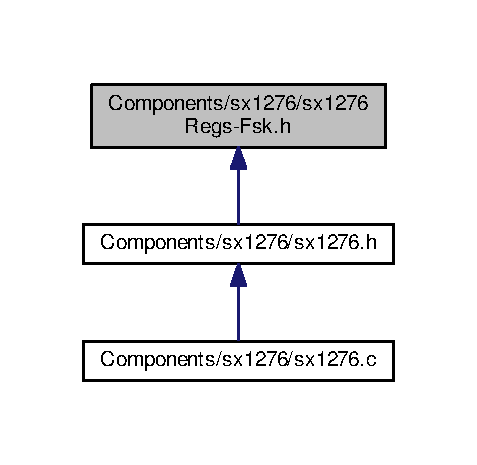
\includegraphics[width=229pt]{sx1276Regs-Fsk_8h__dep__incl}
\end{center}
\end{figure}
\subsection*{Macros}
\begin{DoxyCompactItemize}
\item 
\#define \hyperlink{sx1276Regs-Fsk_8h_a8ed1afe4fdc88a0f2626d9ee783e06e5}{R\+E\+G\+\_\+\+F\+I\+FO}~0x00
\item 
\#define \hyperlink{sx1276Regs-Fsk_8h_af3f25ba8cab1ad2c10ee96089d5a21be}{R\+E\+G\+\_\+\+O\+P\+M\+O\+DE}~0x01
\item 
\#define \hyperlink{sx1276Regs-Fsk_8h_a967024927a998c8b00e76015c0444d11}{R\+E\+G\+\_\+\+B\+I\+T\+R\+A\+T\+E\+M\+SB}~0x02
\item 
\#define \hyperlink{sx1276Regs-Fsk_8h_ab7321068986e253c5e0c4c00f592339b}{R\+E\+G\+\_\+\+B\+I\+T\+R\+A\+T\+E\+L\+SB}~0x03
\item 
\#define \hyperlink{sx1276Regs-Fsk_8h_ac9a9ad053f237a88ac9ef4e9f1eb6902}{R\+E\+G\+\_\+\+F\+D\+E\+V\+M\+SB}~0x04
\item 
\#define \hyperlink{sx1276Regs-Fsk_8h_a41b897af0ba110c4450e54887148acda}{R\+E\+G\+\_\+\+F\+D\+E\+V\+L\+SB}~0x05
\item 
\#define \hyperlink{sx1276Regs-Fsk_8h_a80711d5ed54cc1aa69666b92ea78c353}{R\+E\+G\+\_\+\+F\+R\+F\+M\+SB}~0x06
\item 
\#define \hyperlink{sx1276Regs-Fsk_8h_ad80489ab7d36cc8d9c725ab45f77c731}{R\+E\+G\+\_\+\+F\+R\+F\+M\+ID}~0x07
\item 
\#define \hyperlink{sx1276Regs-Fsk_8h_a3f6b75c6bcb9bb8631cd7fa7151dd934}{R\+E\+G\+\_\+\+F\+R\+F\+L\+SB}~0x08
\item 
\#define \hyperlink{sx1276Regs-Fsk_8h_a36b48e41982d4b0d0b6758a5e1ba398e}{R\+E\+G\+\_\+\+P\+A\+C\+O\+N\+F\+IG}~0x09
\item 
\#define \hyperlink{sx1276Regs-Fsk_8h_aff539bfb169523f9feb34a1d28daaa3f}{R\+E\+G\+\_\+\+P\+A\+R\+A\+MP}~0x0A
\item 
\#define \hyperlink{sx1276Regs-Fsk_8h_a4e0e13619868140039378bb218aa5a3b}{R\+E\+G\+\_\+\+O\+CP}~0x0B
\item 
\#define \hyperlink{sx1276Regs-Fsk_8h_ab08aa4c56ad75b3e715a1115330109ca}{R\+E\+G\+\_\+\+L\+NA}~0x0C
\item 
\#define \hyperlink{sx1276Regs-Fsk_8h_a6bba52e363d49d2783439eb8062d90c8}{R\+E\+G\+\_\+\+R\+X\+C\+O\+N\+F\+IG}~0x0D
\item 
\#define \hyperlink{sx1276Regs-Fsk_8h_a9ba1a67481c3ba0a454cb4873e4db10b}{R\+E\+G\+\_\+\+R\+S\+S\+I\+C\+O\+N\+F\+IG}~0x0E
\item 
\#define \hyperlink{sx1276Regs-Fsk_8h_ad810a0e5aaa761e8edbe804df2e4f5fe}{R\+E\+G\+\_\+\+R\+S\+S\+I\+C\+O\+L\+L\+I\+S\+I\+ON}~0x0F
\item 
\#define \hyperlink{sx1276Regs-Fsk_8h_ab3af0df6e457f5b5f994d1c19dc2642f}{R\+E\+G\+\_\+\+R\+S\+S\+I\+T\+H\+R\+E\+SH}~0x10
\item 
\#define \hyperlink{sx1276Regs-Fsk_8h_a7ff36314652a235acc13fa6ab5504e3d}{R\+E\+G\+\_\+\+R\+S\+S\+I\+V\+A\+L\+UE}~0x11
\item 
\#define \hyperlink{sx1276Regs-Fsk_8h_a1bbbafd83ab10909a8dd5385fd0dfff8}{R\+E\+G\+\_\+\+R\+X\+BW}~0x12
\item 
\#define \hyperlink{sx1276Regs-Fsk_8h_aa4a7b5b5d63e9f8ef8f8dc4d7984753c}{R\+E\+G\+\_\+\+A\+F\+C\+BW}~0x13
\item 
\#define \hyperlink{sx1276Regs-Fsk_8h_a4a6adb6f15f5e4fe71a627d96f6f8141}{R\+E\+G\+\_\+\+O\+O\+K\+P\+E\+AK}~0x14
\item 
\#define \hyperlink{sx1276Regs-Fsk_8h_a585aebf4bf7b6d781ac836ade0f00aad}{R\+E\+G\+\_\+\+O\+O\+K\+F\+IX}~0x15
\item 
\#define \hyperlink{sx1276Regs-Fsk_8h_ad0c870505b9062bb61176ba9076e9b5e}{R\+E\+G\+\_\+\+O\+O\+K\+A\+VG}~0x16
\item 
\#define \hyperlink{sx1276Regs-Fsk_8h_a6a38821b7a89a409d200dbd0420c92c8}{R\+E\+G\+\_\+\+R\+E\+S17}~0x17
\item 
\#define \hyperlink{sx1276Regs-Fsk_8h_a855a1d320f1a948b9210dbd3a7ecc4cc}{R\+E\+G\+\_\+\+R\+E\+S18}~0x18
\item 
\#define \hyperlink{sx1276Regs-Fsk_8h_a1459e2972b36abc24aeed3b664cbe2c1}{R\+E\+G\+\_\+\+R\+E\+S19}~0x19
\item 
\#define \hyperlink{sx1276Regs-Fsk_8h_a04f60f1d03035cf80cebff9648a894c0}{R\+E\+G\+\_\+\+A\+F\+C\+F\+EI}~0x1A
\item 
\#define \hyperlink{sx1276Regs-Fsk_8h_a989d0164e5d5090b39e25506526e0aa5}{R\+E\+G\+\_\+\+A\+F\+C\+M\+SB}~0x1B
\item 
\#define \hyperlink{sx1276Regs-Fsk_8h_a4c64591ff1cb9d48f90c679a6f5985c7}{R\+E\+G\+\_\+\+A\+F\+C\+L\+SB}~0x1C
\item 
\#define \hyperlink{sx1276Regs-Fsk_8h_a99f252ad098770ae36c2947075ba011a}{R\+E\+G\+\_\+\+F\+E\+I\+M\+SB}~0x1D
\item 
\#define \hyperlink{sx1276Regs-Fsk_8h_a02e249f7bd9ca6c91dea006e205bbbe5}{R\+E\+G\+\_\+\+F\+E\+I\+L\+SB}~0x1E
\item 
\#define \hyperlink{sx1276Regs-Fsk_8h_a8acf717d67c4e7f4b92a25653ddb495c}{R\+E\+G\+\_\+\+P\+R\+E\+A\+M\+B\+L\+E\+D\+E\+T\+E\+CT}~0x1F
\item 
\#define \hyperlink{sx1276Regs-Fsk_8h_afa819749e90d0ecb13a5d75f28af5ccb}{R\+E\+G\+\_\+\+R\+X\+T\+I\+M\+E\+O\+U\+T1}~0x20
\item 
\#define \hyperlink{sx1276Regs-Fsk_8h_aa5870403dc3e6ba5cb5212423051e18a}{R\+E\+G\+\_\+\+R\+X\+T\+I\+M\+E\+O\+U\+T2}~0x21
\item 
\#define \hyperlink{sx1276Regs-Fsk_8h_a8167beac9018acd4f54b530176170145}{R\+E\+G\+\_\+\+R\+X\+T\+I\+M\+E\+O\+U\+T3}~0x22
\item 
\#define \hyperlink{sx1276Regs-Fsk_8h_a8ee126fae09fa47e0ef722dc43a4dc22}{R\+E\+G\+\_\+\+R\+X\+D\+E\+L\+AY}~0x23
\item 
\#define \hyperlink{sx1276Regs-Fsk_8h_a1edb093ed684495473ecd2e97e3a49c2}{R\+E\+G\+\_\+\+O\+SC}~0x24
\item 
\#define \hyperlink{sx1276Regs-Fsk_8h_ab8a433a9dd9c4cebe485d1a1b49cfd4b}{R\+E\+G\+\_\+\+P\+R\+E\+A\+M\+B\+L\+E\+M\+SB}~0x25
\item 
\#define \hyperlink{sx1276Regs-Fsk_8h_a342040215f26acdefd5c95ec7c8ce828}{R\+E\+G\+\_\+\+P\+R\+E\+A\+M\+B\+L\+E\+L\+SB}~0x26
\item 
\#define \hyperlink{sx1276Regs-Fsk_8h_ae80bd3142a5c405bf7063ac7b0e8e101}{R\+E\+G\+\_\+\+S\+Y\+N\+C\+C\+O\+N\+F\+IG}~0x27
\item 
\#define \hyperlink{sx1276Regs-Fsk_8h_a4d0160e654656b6cd6426c295c8e131b}{R\+E\+G\+\_\+\+S\+Y\+N\+C\+V\+A\+L\+U\+E1}~0x28
\item 
\#define \hyperlink{sx1276Regs-Fsk_8h_a840d780f6d455dc828e2ec8217e9043a}{R\+E\+G\+\_\+\+S\+Y\+N\+C\+V\+A\+L\+U\+E2}~0x29
\item 
\#define \hyperlink{sx1276Regs-Fsk_8h_af89062529e96d32eecd0f89963d52adf}{R\+E\+G\+\_\+\+S\+Y\+N\+C\+V\+A\+L\+U\+E3}~0x2A
\item 
\#define \hyperlink{sx1276Regs-Fsk_8h_a9768416ceaebbdeab3fee291f351a98f}{R\+E\+G\+\_\+\+S\+Y\+N\+C\+V\+A\+L\+U\+E4}~0x2B
\item 
\#define \hyperlink{sx1276Regs-Fsk_8h_a834570d54f8b7370a5d42fc180650c14}{R\+E\+G\+\_\+\+S\+Y\+N\+C\+V\+A\+L\+U\+E5}~0x2C
\item 
\#define \hyperlink{sx1276Regs-Fsk_8h_a4e2e2802416f6a445a355828764363e2}{R\+E\+G\+\_\+\+S\+Y\+N\+C\+V\+A\+L\+U\+E6}~0x2D
\item 
\#define \hyperlink{sx1276Regs-Fsk_8h_ac276ab640ba22f4edb9cc206567f1e22}{R\+E\+G\+\_\+\+S\+Y\+N\+C\+V\+A\+L\+U\+E7}~0x2E
\item 
\#define \hyperlink{sx1276Regs-Fsk_8h_ab29ed95bcf10e2b561a2400806344f81}{R\+E\+G\+\_\+\+S\+Y\+N\+C\+V\+A\+L\+U\+E8}~0x2F
\item 
\#define \hyperlink{sx1276Regs-Fsk_8h_a035c91c3eea7209c78ac5bda775940cc}{R\+E\+G\+\_\+\+P\+A\+C\+K\+E\+T\+C\+O\+N\+F\+I\+G1}~0x30
\item 
\#define \hyperlink{sx1276Regs-Fsk_8h_a519d7b5db6ab8bb6013226eaef9756c8}{R\+E\+G\+\_\+\+P\+A\+C\+K\+E\+T\+C\+O\+N\+F\+I\+G2}~0x31
\item 
\#define \hyperlink{sx1276Regs-Fsk_8h_ac1f66aa74c41653c8d30ce6b92af3769}{R\+E\+G\+\_\+\+P\+A\+Y\+L\+O\+A\+D\+L\+E\+N\+G\+TH}~0x32
\item 
\#define \hyperlink{sx1276Regs-Fsk_8h_aa62099ad5a5d4b5967f1ded180d5f685}{R\+E\+G\+\_\+\+N\+O\+D\+E\+A\+D\+RS}~0x33
\item 
\#define \hyperlink{sx1276Regs-Fsk_8h_a5c96b6f1a3e95a80f700d3a0c8ed5742}{R\+E\+G\+\_\+\+B\+R\+O\+A\+D\+C\+A\+S\+T\+A\+D\+RS}~0x34
\item 
\#define \hyperlink{sx1276Regs-Fsk_8h_a18b41b1ddfbe6eb514f74431b5d76792}{R\+E\+G\+\_\+\+F\+I\+F\+O\+T\+H\+R\+E\+SH}~0x35
\item 
\#define \hyperlink{sx1276Regs-Fsk_8h_aed3f5e12a0c953d12aacbc1146f2dde8}{R\+E\+G\+\_\+\+S\+E\+Q\+C\+O\+N\+F\+I\+G1}~0x36
\item 
\#define \hyperlink{sx1276Regs-Fsk_8h_a93a8f2fecd93790802eab65f9685dfb6}{R\+E\+G\+\_\+\+S\+E\+Q\+C\+O\+N\+F\+I\+G2}~0x37
\item 
\#define \hyperlink{sx1276Regs-Fsk_8h_a92529ed06adfae1625c5300057a88f23}{R\+E\+G\+\_\+\+T\+I\+M\+E\+R\+R\+E\+S\+OL}~0x38
\item 
\#define \hyperlink{sx1276Regs-Fsk_8h_a748e83f19ce0c442f47ff56c3ae2ae1c}{R\+E\+G\+\_\+\+T\+I\+M\+E\+R1\+C\+O\+EF}~0x39
\item 
\#define \hyperlink{sx1276Regs-Fsk_8h_a35594318e2541ff55e79e1ce8d52ab8a}{R\+E\+G\+\_\+\+T\+I\+M\+E\+R2\+C\+O\+EF}~0x3A
\item 
\#define \hyperlink{sx1276Regs-Fsk_8h_aeb557bae3e3e5ffb390a6f6a61ac686d}{R\+E\+G\+\_\+\+I\+M\+A\+G\+E\+C\+AL}~0x3B
\item 
\#define \hyperlink{sx1276Regs-Fsk_8h_ad3b0b6d8d5d3de58e5d56ce84e667b20}{R\+E\+G\+\_\+\+T\+E\+MP}~0x3C
\item 
\#define \hyperlink{sx1276Regs-Fsk_8h_afbb15f7aeaefcb5994a64fff237025f9}{R\+E\+G\+\_\+\+L\+O\+W\+B\+AT}~0x3D
\item 
\#define \hyperlink{sx1276Regs-Fsk_8h_a271d978a9b14435dc5f3d8f3ac9b8951}{R\+E\+G\+\_\+\+I\+R\+Q\+F\+L\+A\+G\+S1}~0x3E
\item 
\#define \hyperlink{sx1276Regs-Fsk_8h_ae93c6dbbf26ea297ba04cbe39c116ff3}{R\+E\+G\+\_\+\+I\+R\+Q\+F\+L\+A\+G\+S2}~0x3F
\item 
\#define \hyperlink{sx1276Regs-Fsk_8h_ac16d5678e98fa6ab73655240a11f9b69}{R\+E\+G\+\_\+\+D\+I\+O\+M\+A\+P\+P\+I\+N\+G1}~0x40
\item 
\#define \hyperlink{sx1276Regs-Fsk_8h_aec8b1ddf72925f502675593fabcc469f}{R\+E\+G\+\_\+\+D\+I\+O\+M\+A\+P\+P\+I\+N\+G2}~0x41
\item 
\#define \hyperlink{sx1276Regs-Fsk_8h_aa7075c0ae73420685bb4278ee580f3fa}{R\+E\+G\+\_\+\+V\+E\+R\+S\+I\+ON}~0x42
\item 
\#define \hyperlink{sx1276Regs-Fsk_8h_a6a8f2748b149c14533e877f06e4720f3}{R\+E\+G\+\_\+\+P\+L\+L\+H\+OP}~0x44
\item 
\#define \hyperlink{sx1276Regs-Fsk_8h_a57f595889f6a6af755ecc9b3bb5b4c3d}{R\+E\+G\+\_\+\+T\+C\+XO}~0x4B
\item 
\#define \hyperlink{sx1276Regs-Fsk_8h_ad64f0f69f548f51e16be4a9a07d980cd}{R\+E\+G\+\_\+\+P\+A\+D\+AC}~0x4D
\item 
\#define \hyperlink{sx1276Regs-Fsk_8h_a1c2bc2d26e0f676a4f012e975f1d86f2}{R\+E\+G\+\_\+\+F\+O\+R\+M\+E\+R\+T\+E\+MP}~0x5B
\item 
\#define \hyperlink{sx1276Regs-Fsk_8h_a1e0117bd4c660d60afc9d119840f9e26}{R\+E\+G\+\_\+\+B\+I\+T\+R\+A\+T\+E\+F\+R\+AC}~0x5D
\item 
\#define \hyperlink{sx1276Regs-Fsk_8h_a3dc004091d7cb3015aff5967e09b77d8}{R\+E\+G\+\_\+\+A\+G\+C\+R\+EF}~0x61
\item 
\#define \hyperlink{sx1276Regs-Fsk_8h_a1d0f8f390ec3b351e10e37e7258ca6df}{R\+E\+G\+\_\+\+A\+G\+C\+T\+H\+R\+E\+S\+H1}~0x62
\item 
\#define \hyperlink{sx1276Regs-Fsk_8h_ac3b7b366f9a287e32a0be6724909f644}{R\+E\+G\+\_\+\+A\+G\+C\+T\+H\+R\+E\+S\+H2}~0x63
\item 
\#define \hyperlink{sx1276Regs-Fsk_8h_a1686f2ccb6d060e425194a9414fd7ca3}{R\+E\+G\+\_\+\+A\+G\+C\+T\+H\+R\+E\+S\+H3}~0x64
\item 
\#define \hyperlink{sx1276Regs-Fsk_8h_aa5110ddd4aaa720908be259b5a4af489}{R\+E\+G\+\_\+\+P\+LL}~0x70
\item 
\#define \hyperlink{sx1276Regs-Fsk_8h_afd99a116c626b5579054d37c640e175a}{R\+F\+\_\+\+O\+P\+M\+O\+D\+E\+\_\+\+L\+O\+N\+G\+R\+A\+N\+G\+E\+M\+O\+D\+E\+\_\+\+M\+A\+SK}~0x7F
\item 
\#define \hyperlink{sx1276Regs-Fsk_8h_a856e634d884238e300fdf87a2557d670}{R\+F\+\_\+\+O\+P\+M\+O\+D\+E\+\_\+\+L\+O\+N\+G\+R\+A\+N\+G\+E\+M\+O\+D\+E\+\_\+\+O\+FF}~0x00
\item 
\#define \hyperlink{sx1276Regs-Fsk_8h_a1775751bd57cbba5d752ebf2e03c6e1b}{R\+F\+\_\+\+O\+P\+M\+O\+D\+E\+\_\+\+L\+O\+N\+G\+R\+A\+N\+G\+E\+M\+O\+D\+E\+\_\+\+ON}~0x80
\item 
\#define \hyperlink{sx1276Regs-Fsk_8h_a9b3d405d931ad505308b89d2fa029dbb}{R\+F\+\_\+\+O\+P\+M\+O\+D\+E\+\_\+\+M\+O\+D\+U\+L\+A\+T\+I\+O\+N\+T\+Y\+P\+E\+\_\+\+M\+A\+SK}~0x9F
\item 
\#define \hyperlink{sx1276Regs-Fsk_8h_af4f3f4b19fd43491f270fcee634edd13}{R\+F\+\_\+\+O\+P\+M\+O\+D\+E\+\_\+\+M\+O\+D\+U\+L\+A\+T\+I\+O\+N\+T\+Y\+P\+E\+\_\+\+F\+SK}~0x00
\item 
\#define \hyperlink{sx1276Regs-Fsk_8h_af6fe2f62d8ec55fcf40c73ae24bc54ae}{R\+F\+\_\+\+O\+P\+M\+O\+D\+E\+\_\+\+M\+O\+D\+U\+L\+A\+T\+I\+O\+N\+T\+Y\+P\+E\+\_\+\+O\+OK}~0x20
\item 
\#define \hyperlink{sx1276Regs-Fsk_8h_a1b851bfa8cc641cd5a2a0805df4f4762}{R\+F\+\_\+\+O\+P\+M\+O\+D\+E\+\_\+\+M\+O\+D\+U\+L\+A\+T\+I\+O\+N\+S\+H\+A\+P\+I\+N\+G\+\_\+\+M\+A\+SK}~0x\+E7
\item 
\#define \hyperlink{sx1276Regs-Fsk_8h_a1a589ce58d8c5fb2da244d4829d11a3f}{R\+F\+\_\+\+O\+P\+M\+O\+D\+E\+\_\+\+M\+O\+D\+U\+L\+A\+T\+I\+O\+N\+S\+H\+A\+P\+I\+N\+G\+\_\+00}~0x00
\item 
\#define \hyperlink{sx1276Regs-Fsk_8h_a19fca1c14eed0e9a8879aaef7a27e05f}{R\+F\+\_\+\+O\+P\+M\+O\+D\+E\+\_\+\+M\+O\+D\+U\+L\+A\+T\+I\+O\+N\+S\+H\+A\+P\+I\+N\+G\+\_\+01}~0x08
\item 
\#define \hyperlink{sx1276Regs-Fsk_8h_a07bd0112f429ed1340afabbb6d511da3}{R\+F\+\_\+\+O\+P\+M\+O\+D\+E\+\_\+\+M\+O\+D\+U\+L\+A\+T\+I\+O\+N\+S\+H\+A\+P\+I\+N\+G\+\_\+10}~0x10
\item 
\#define \hyperlink{sx1276Regs-Fsk_8h_a9f1f93b87462b90bcbccba6a26400c89}{R\+F\+\_\+\+O\+P\+M\+O\+D\+E\+\_\+\+M\+O\+D\+U\+L\+A\+T\+I\+O\+N\+S\+H\+A\+P\+I\+N\+G\+\_\+11}~0x18
\item 
\#define \hyperlink{sx1276Regs-Fsk_8h_a85461827ea27e5138c9198c75f1bdf6e}{R\+F\+\_\+\+O\+P\+M\+O\+D\+E\+\_\+\+M\+A\+SK}~0x\+F8
\item 
\#define \hyperlink{sx1276Regs-Fsk_8h_a2b5cd905a9116a8a462c28a2d17c483a}{R\+F\+\_\+\+O\+P\+M\+O\+D\+E\+\_\+\+S\+L\+E\+EP}~0x00
\item 
\#define \hyperlink{sx1276Regs-Fsk_8h_a8061431d06917243c6409c4a014c3592}{R\+F\+\_\+\+O\+P\+M\+O\+D\+E\+\_\+\+S\+T\+A\+N\+D\+BY}~0x01
\item 
\#define \hyperlink{sx1276Regs-Fsk_8h_ab384b4d4a5a2e55a8a6eadf18e00e8db}{R\+F\+\_\+\+O\+P\+M\+O\+D\+E\+\_\+\+S\+Y\+N\+T\+H\+E\+S\+I\+Z\+E\+R\+\_\+\+TX}~0x02
\item 
\#define \hyperlink{sx1276Regs-Fsk_8h_a9851bc9741460e2c48415a59f9e3f5ba}{R\+F\+\_\+\+O\+P\+M\+O\+D\+E\+\_\+\+T\+R\+A\+N\+S\+M\+I\+T\+T\+ER}~0x03
\item 
\#define \hyperlink{sx1276Regs-Fsk_8h_a7257f5b516d9fe4c292a87c569ac1519}{R\+F\+\_\+\+O\+P\+M\+O\+D\+E\+\_\+\+S\+Y\+N\+T\+H\+E\+S\+I\+Z\+E\+R\+\_\+\+RX}~0x04
\item 
\#define \hyperlink{sx1276Regs-Fsk_8h_a7a13dffe3a61d783cdbbb0ac11cc85b2}{R\+F\+\_\+\+O\+P\+M\+O\+D\+E\+\_\+\+R\+E\+C\+E\+I\+V\+ER}~0x05
\item 
\#define \hyperlink{sx1276Regs-Fsk_8h_abefe1b1960c632cccac981eed31ddfdf}{R\+F\+\_\+\+B\+I\+T\+R\+A\+T\+E\+M\+S\+B\+\_\+1200\+\_\+\+B\+PS}~0x68
\item 
\#define \hyperlink{sx1276Regs-Fsk_8h_a61be3af220402958165d9e69f7f506c6}{R\+F\+\_\+\+B\+I\+T\+R\+A\+T\+E\+L\+S\+B\+\_\+1200\+\_\+\+B\+PS}~0x2B
\item 
\#define \hyperlink{sx1276Regs-Fsk_8h_af1a5b1f28fc382c9df4d6e482b448c3c}{R\+F\+\_\+\+B\+I\+T\+R\+A\+T\+E\+M\+S\+B\+\_\+2400\+\_\+\+B\+PS}~0x34
\item 
\#define \hyperlink{sx1276Regs-Fsk_8h_a9341847d10e8210454bc8c5abcbef3e3}{R\+F\+\_\+\+B\+I\+T\+R\+A\+T\+E\+L\+S\+B\+\_\+2400\+\_\+\+B\+PS}~0x15
\item 
\#define \hyperlink{sx1276Regs-Fsk_8h_a3fbe8a73f4b0a021159cd8046e9e1959}{R\+F\+\_\+\+B\+I\+T\+R\+A\+T\+E\+M\+S\+B\+\_\+4800\+\_\+\+B\+PS}~0x1A
\item 
\#define \hyperlink{sx1276Regs-Fsk_8h_a37dfb650a26879afa9a8aa036507b189}{R\+F\+\_\+\+B\+I\+T\+R\+A\+T\+E\+L\+S\+B\+\_\+4800\+\_\+\+B\+PS}~0x0B
\item 
\#define \hyperlink{sx1276Regs-Fsk_8h_ae69250b1621744d9da30c06f56d0f483}{R\+F\+\_\+\+B\+I\+T\+R\+A\+T\+E\+M\+S\+B\+\_\+9600\+\_\+\+B\+PS}~0x0D
\item 
\#define \hyperlink{sx1276Regs-Fsk_8h_ad137bc838a75f376cf1b9be4f53e6eb7}{R\+F\+\_\+\+B\+I\+T\+R\+A\+T\+E\+L\+S\+B\+\_\+9600\+\_\+\+B\+PS}~0x05
\item 
\#define \hyperlink{sx1276Regs-Fsk_8h_a1e8f56770ecc5d5f7264a7029f7ae2c3}{R\+F\+\_\+\+B\+I\+T\+R\+A\+T\+E\+M\+S\+B\+\_\+15000\+\_\+\+B\+PS}~0x08
\item 
\#define \hyperlink{sx1276Regs-Fsk_8h_a60340fe3a748b8e02ed6ebbf2426d620}{R\+F\+\_\+\+B\+I\+T\+R\+A\+T\+E\+L\+S\+B\+\_\+15000\+\_\+\+B\+PS}~0x55
\item 
\#define \hyperlink{sx1276Regs-Fsk_8h_aeec19a1a2418cf8ed29ac2ce61ebbe76}{R\+F\+\_\+\+B\+I\+T\+R\+A\+T\+E\+M\+S\+B\+\_\+19200\+\_\+\+B\+PS}~0x06
\item 
\#define \hyperlink{sx1276Regs-Fsk_8h_a4f1ddd00d5777887dc4b68b3711df3c9}{R\+F\+\_\+\+B\+I\+T\+R\+A\+T\+E\+L\+S\+B\+\_\+19200\+\_\+\+B\+PS}~0x83
\item 
\#define \hyperlink{sx1276Regs-Fsk_8h_a041c9eb73ab4c25e3ed8a25303a49ad0}{R\+F\+\_\+\+B\+I\+T\+R\+A\+T\+E\+M\+S\+B\+\_\+38400\+\_\+\+B\+PS}~0x03
\item 
\#define \hyperlink{sx1276Regs-Fsk_8h_a71ea2cd6143ebf9bf63a7118064a471f}{R\+F\+\_\+\+B\+I\+T\+R\+A\+T\+E\+L\+S\+B\+\_\+38400\+\_\+\+B\+PS}~0x41
\item 
\#define \hyperlink{sx1276Regs-Fsk_8h_a8e3881281736c31ce8b72b51e801b49d}{R\+F\+\_\+\+B\+I\+T\+R\+A\+T\+E\+M\+S\+B\+\_\+76800\+\_\+\+B\+PS}~0x01
\item 
\#define \hyperlink{sx1276Regs-Fsk_8h_ae22ca1c6a214c62d298eb1f6d76ba092}{R\+F\+\_\+\+B\+I\+T\+R\+A\+T\+E\+L\+S\+B\+\_\+76800\+\_\+\+B\+PS}~0x\+A1
\item 
\#define \hyperlink{sx1276Regs-Fsk_8h_a68aec0128102e04f2699befbf244f5ec}{R\+F\+\_\+\+B\+I\+T\+R\+A\+T\+E\+M\+S\+B\+\_\+153600\+\_\+\+B\+PS}~0x00
\item 
\#define \hyperlink{sx1276Regs-Fsk_8h_a918d453d557cfd2e89c2310591290ef6}{R\+F\+\_\+\+B\+I\+T\+R\+A\+T\+E\+L\+S\+B\+\_\+153600\+\_\+\+B\+PS}~0x\+D0
\item 
\#define \hyperlink{sx1276Regs-Fsk_8h_a5c8867e729d049e6b01d95f17daeaa43}{R\+F\+\_\+\+B\+I\+T\+R\+A\+T\+E\+M\+S\+B\+\_\+57600\+\_\+\+B\+PS}~0x02
\item 
\#define \hyperlink{sx1276Regs-Fsk_8h_a4b990574403a3171c4bf1ef56f87076c}{R\+F\+\_\+\+B\+I\+T\+R\+A\+T\+E\+L\+S\+B\+\_\+57600\+\_\+\+B\+PS}~0x2C
\item 
\#define \hyperlink{sx1276Regs-Fsk_8h_a4f3568a645d981cc5d56d5892fd79fea}{R\+F\+\_\+\+B\+I\+T\+R\+A\+T\+E\+M\+S\+B\+\_\+115200\+\_\+\+B\+PS}~0x01
\item 
\#define \hyperlink{sx1276Regs-Fsk_8h_a6677546d2936ed5f36a259f13c123d00}{R\+F\+\_\+\+B\+I\+T\+R\+A\+T\+E\+L\+S\+B\+\_\+115200\+\_\+\+B\+PS}~0x16
\item 
\#define \hyperlink{sx1276Regs-Fsk_8h_a8d2d2c7221965aeac9af067528723746}{R\+F\+\_\+\+B\+I\+T\+R\+A\+T\+E\+M\+S\+B\+\_\+12500\+\_\+\+B\+PS}~0x0A
\item 
\#define \hyperlink{sx1276Regs-Fsk_8h_a382c67b25793c0884e7bfe662dfb06c6}{R\+F\+\_\+\+B\+I\+T\+R\+A\+T\+E\+L\+S\+B\+\_\+12500\+\_\+\+B\+PS}~0x00
\item 
\#define \hyperlink{sx1276Regs-Fsk_8h_a783ebd0eeb85cb90ed09736f058122ed}{R\+F\+\_\+\+B\+I\+T\+R\+A\+T\+E\+M\+S\+B\+\_\+25000\+\_\+\+B\+PS}~0x05
\item 
\#define \hyperlink{sx1276Regs-Fsk_8h_af7a1f67d376fd019e9b883a080b35700}{R\+F\+\_\+\+B\+I\+T\+R\+A\+T\+E\+L\+S\+B\+\_\+25000\+\_\+\+B\+PS}~0x00
\item 
\#define \hyperlink{sx1276Regs-Fsk_8h_a7b42c7402e7d73f2e75d753085badf7a}{R\+F\+\_\+\+B\+I\+T\+R\+A\+T\+E\+M\+S\+B\+\_\+50000\+\_\+\+B\+PS}~0x02
\item 
\#define \hyperlink{sx1276Regs-Fsk_8h_a1780bbfac40913821e859a35c0a7eae2}{R\+F\+\_\+\+B\+I\+T\+R\+A\+T\+E\+L\+S\+B\+\_\+50000\+\_\+\+B\+PS}~0x80
\item 
\#define \hyperlink{sx1276Regs-Fsk_8h_a899b8e6397e082b4d95f589ba51093b0}{R\+F\+\_\+\+B\+I\+T\+R\+A\+T\+E\+M\+S\+B\+\_\+100000\+\_\+\+B\+PS}~0x01
\item 
\#define \hyperlink{sx1276Regs-Fsk_8h_ac8a775e0079f97d0da847bcbc743f8b8}{R\+F\+\_\+\+B\+I\+T\+R\+A\+T\+E\+L\+S\+B\+\_\+100000\+\_\+\+B\+PS}~0x40
\item 
\#define \hyperlink{sx1276Regs-Fsk_8h_adb3227e86cec303479803ee36c94dc12}{R\+F\+\_\+\+B\+I\+T\+R\+A\+T\+E\+M\+S\+B\+\_\+150000\+\_\+\+B\+PS}~0x00
\item 
\#define \hyperlink{sx1276Regs-Fsk_8h_a4c354668226a9b7cbc899d1571eb7f6a}{R\+F\+\_\+\+B\+I\+T\+R\+A\+T\+E\+L\+S\+B\+\_\+150000\+\_\+\+B\+PS}~0x\+D5
\item 
\#define \hyperlink{sx1276Regs-Fsk_8h_a2820d9407f3f886ccc4b95f37bdba43a}{R\+F\+\_\+\+B\+I\+T\+R\+A\+T\+E\+M\+S\+B\+\_\+200000\+\_\+\+B\+PS}~0x00
\item 
\#define \hyperlink{sx1276Regs-Fsk_8h_a5dc775df5325cee5e4f068777ec7d0ce}{R\+F\+\_\+\+B\+I\+T\+R\+A\+T\+E\+L\+S\+B\+\_\+200000\+\_\+\+B\+PS}~0x\+A0
\item 
\#define \hyperlink{sx1276Regs-Fsk_8h_a2929fca60be7a159f4f0b3768f60d811}{R\+F\+\_\+\+B\+I\+T\+R\+A\+T\+E\+M\+S\+B\+\_\+250000\+\_\+\+B\+PS}~0x00
\item 
\#define \hyperlink{sx1276Regs-Fsk_8h_a39ce2c4b4f89ca91ee4a9a943341a75f}{R\+F\+\_\+\+B\+I\+T\+R\+A\+T\+E\+L\+S\+B\+\_\+250000\+\_\+\+B\+PS}~0x80
\item 
\#define \hyperlink{sx1276Regs-Fsk_8h_a7110c5c5081018aa2856943a0cf1223c}{R\+F\+\_\+\+B\+I\+T\+R\+A\+T\+E\+M\+S\+B\+\_\+32768\+\_\+\+B\+PS}~0x03
\item 
\#define \hyperlink{sx1276Regs-Fsk_8h_a358a84803ccf3e4c4896cdbd43576c08}{R\+F\+\_\+\+B\+I\+T\+R\+A\+T\+E\+L\+S\+B\+\_\+32768\+\_\+\+B\+PS}~0x\+D1
\item 
\#define \hyperlink{sx1276Regs-Fsk_8h_a5f494883fb5d77b75be547962cc3bc55}{R\+F\+\_\+\+F\+D\+E\+V\+M\+S\+B\+\_\+2000\+\_\+\+HZ}~0x00
\item 
\#define \hyperlink{sx1276Regs-Fsk_8h_acf567929b56d3921b2d717142b29275b}{R\+F\+\_\+\+F\+D\+E\+V\+L\+S\+B\+\_\+2000\+\_\+\+HZ}~0x21
\item 
\#define \hyperlink{sx1276Regs-Fsk_8h_ae6ae0e5b1aa1a2bdd92b3c9fccdb533c}{R\+F\+\_\+\+F\+D\+E\+V\+M\+S\+B\+\_\+5000\+\_\+\+HZ}~0x00
\item 
\#define \hyperlink{sx1276Regs-Fsk_8h_adafffdefc88466fdb255869839356960}{R\+F\+\_\+\+F\+D\+E\+V\+L\+S\+B\+\_\+5000\+\_\+\+HZ}~0x52
\item 
\#define \hyperlink{sx1276Regs-Fsk_8h_a687bcf3879dd873acbd21cba5b7142c5}{R\+F\+\_\+\+F\+D\+E\+V\+M\+S\+B\+\_\+10000\+\_\+\+HZ}~0x00
\item 
\#define \hyperlink{sx1276Regs-Fsk_8h_a0751e1ea52818613b7a5e3476607f646}{R\+F\+\_\+\+F\+D\+E\+V\+L\+S\+B\+\_\+10000\+\_\+\+HZ}~0x\+A4
\item 
\#define \hyperlink{sx1276Regs-Fsk_8h_a91093fabca4892b315095dc0283828c7}{R\+F\+\_\+\+F\+D\+E\+V\+M\+S\+B\+\_\+15000\+\_\+\+HZ}~0x00
\item 
\#define \hyperlink{sx1276Regs-Fsk_8h_a5331d1f2a7cd8c568218d901d2a388ce}{R\+F\+\_\+\+F\+D\+E\+V\+L\+S\+B\+\_\+15000\+\_\+\+HZ}~0x\+F6
\item 
\#define \hyperlink{sx1276Regs-Fsk_8h_ada7253b158b4a51d4a8621eff8d3aa59}{R\+F\+\_\+\+F\+D\+E\+V\+M\+S\+B\+\_\+20000\+\_\+\+HZ}~0x01
\item 
\#define \hyperlink{sx1276Regs-Fsk_8h_a6e922112d9f9ada8500acab833bec19d}{R\+F\+\_\+\+F\+D\+E\+V\+L\+S\+B\+\_\+20000\+\_\+\+HZ}~0x48
\item 
\#define \hyperlink{sx1276Regs-Fsk_8h_a93a967f33b1732e004831862b3d4964f}{R\+F\+\_\+\+F\+D\+E\+V\+M\+S\+B\+\_\+25000\+\_\+\+HZ}~0x01
\item 
\#define \hyperlink{sx1276Regs-Fsk_8h_a391d42e4ff6fa112df9198fb1a1803fe}{R\+F\+\_\+\+F\+D\+E\+V\+L\+S\+B\+\_\+25000\+\_\+\+HZ}~0x9A
\item 
\#define \hyperlink{sx1276Regs-Fsk_8h_a6b95e0d91882f1c75092a944ccdf8952}{R\+F\+\_\+\+F\+D\+E\+V\+M\+S\+B\+\_\+30000\+\_\+\+HZ}~0x01
\item 
\#define \hyperlink{sx1276Regs-Fsk_8h_a30c6d67de342780865db12984208b286}{R\+F\+\_\+\+F\+D\+E\+V\+L\+S\+B\+\_\+30000\+\_\+\+HZ}~0x\+EC
\item 
\#define \hyperlink{sx1276Regs-Fsk_8h_aae123662302055b52008db80777f3bad}{R\+F\+\_\+\+F\+D\+E\+V\+M\+S\+B\+\_\+35000\+\_\+\+HZ}~0x02
\item 
\#define \hyperlink{sx1276Regs-Fsk_8h_ae12db3f305913ae3a16466507fdd3d3c}{R\+F\+\_\+\+F\+D\+E\+V\+L\+S\+B\+\_\+35000\+\_\+\+HZ}~0x3D
\item 
\#define \hyperlink{sx1276Regs-Fsk_8h_aa12a12d2a93e1a5c35134219f35bb51c}{R\+F\+\_\+\+F\+D\+E\+V\+M\+S\+B\+\_\+40000\+\_\+\+HZ}~0x02
\item 
\#define \hyperlink{sx1276Regs-Fsk_8h_a635b9754fb64e7fa3d62a0eb3a00e086}{R\+F\+\_\+\+F\+D\+E\+V\+L\+S\+B\+\_\+40000\+\_\+\+HZ}~0x8F
\item 
\#define \hyperlink{sx1276Regs-Fsk_8h_a5e36011fe2f0d8bee1bd3aa9a928c18c}{R\+F\+\_\+\+F\+D\+E\+V\+M\+S\+B\+\_\+45000\+\_\+\+HZ}~0x02
\item 
\#define \hyperlink{sx1276Regs-Fsk_8h_a8e69ee5a2729700dda58111180fae357}{R\+F\+\_\+\+F\+D\+E\+V\+L\+S\+B\+\_\+45000\+\_\+\+HZ}~0x\+E1
\item 
\#define \hyperlink{sx1276Regs-Fsk_8h_a2d77a912cc45a97d9fffaeafa791b186}{R\+F\+\_\+\+F\+D\+E\+V\+M\+S\+B\+\_\+50000\+\_\+\+HZ}~0x03
\item 
\#define \hyperlink{sx1276Regs-Fsk_8h_a1675346ade9c8f671aac79a317512699}{R\+F\+\_\+\+F\+D\+E\+V\+L\+S\+B\+\_\+50000\+\_\+\+HZ}~0x33
\item 
\#define \hyperlink{sx1276Regs-Fsk_8h_a2727b4b04f0a27d9f370c8f2b47e81fb}{R\+F\+\_\+\+F\+D\+E\+V\+M\+S\+B\+\_\+55000\+\_\+\+HZ}~0x03
\item 
\#define \hyperlink{sx1276Regs-Fsk_8h_a01b1b43aab91e76e84d00af78699ceba}{R\+F\+\_\+\+F\+D\+E\+V\+L\+S\+B\+\_\+55000\+\_\+\+HZ}~0x85
\item 
\#define \hyperlink{sx1276Regs-Fsk_8h_a0ca702dda690369e62b5225d3e5425e8}{R\+F\+\_\+\+F\+D\+E\+V\+M\+S\+B\+\_\+60000\+\_\+\+HZ}~0x03
\item 
\#define \hyperlink{sx1276Regs-Fsk_8h_ab739890a1c4948ba9df80139f9e90c66}{R\+F\+\_\+\+F\+D\+E\+V\+L\+S\+B\+\_\+60000\+\_\+\+HZ}~0x\+D7
\item 
\#define \hyperlink{sx1276Regs-Fsk_8h_a1d9bb9563e152c76f7cbb9df5e1b36c4}{R\+F\+\_\+\+F\+D\+E\+V\+M\+S\+B\+\_\+65000\+\_\+\+HZ}~0x04
\item 
\#define \hyperlink{sx1276Regs-Fsk_8h_a8036d3d91106128102f59ddecacd4dc3}{R\+F\+\_\+\+F\+D\+E\+V\+L\+S\+B\+\_\+65000\+\_\+\+HZ}~0x29
\item 
\#define \hyperlink{sx1276Regs-Fsk_8h_a3e130dcdc84aa5685b7bc35edf6027f2}{R\+F\+\_\+\+F\+D\+E\+V\+M\+S\+B\+\_\+70000\+\_\+\+HZ}~0x04
\item 
\#define \hyperlink{sx1276Regs-Fsk_8h_af2c378fd0b423a7ab42424b045402936}{R\+F\+\_\+\+F\+D\+E\+V\+L\+S\+B\+\_\+70000\+\_\+\+HZ}~0x7B
\item 
\#define \hyperlink{sx1276Regs-Fsk_8h_a95625bf09af0cd2a50f00f182a14746d}{R\+F\+\_\+\+F\+D\+E\+V\+M\+S\+B\+\_\+75000\+\_\+\+HZ}~0x04
\item 
\#define \hyperlink{sx1276Regs-Fsk_8h_a556565ac523c78650661dce1450dcaf7}{R\+F\+\_\+\+F\+D\+E\+V\+L\+S\+B\+\_\+75000\+\_\+\+HZ}~0x\+CD
\item 
\#define \hyperlink{sx1276Regs-Fsk_8h_af8cf1be1a66c7f6f63c4c73a2603657a}{R\+F\+\_\+\+F\+D\+E\+V\+M\+S\+B\+\_\+80000\+\_\+\+HZ}~0x05
\item 
\#define \hyperlink{sx1276Regs-Fsk_8h_a28c9def64a8f7e81619124df236fb932}{R\+F\+\_\+\+F\+D\+E\+V\+L\+S\+B\+\_\+80000\+\_\+\+HZ}~0x1F
\item 
\#define \hyperlink{sx1276Regs-Fsk_8h_a357181556a2104789f589fa736b3fbad}{R\+F\+\_\+\+F\+D\+E\+V\+M\+S\+B\+\_\+85000\+\_\+\+HZ}~0x05
\item 
\#define \hyperlink{sx1276Regs-Fsk_8h_abd3148b49d4c38af8373bd6915742f61}{R\+F\+\_\+\+F\+D\+E\+V\+L\+S\+B\+\_\+85000\+\_\+\+HZ}~0x71
\item 
\#define \hyperlink{sx1276Regs-Fsk_8h_a61741067e7b6adeb71872ead6d569729}{R\+F\+\_\+\+F\+D\+E\+V\+M\+S\+B\+\_\+90000\+\_\+\+HZ}~0x05
\item 
\#define \hyperlink{sx1276Regs-Fsk_8h_a7b621f874a4cde1cff39524f75238242}{R\+F\+\_\+\+F\+D\+E\+V\+L\+S\+B\+\_\+90000\+\_\+\+HZ}~0x\+C3
\item 
\#define \hyperlink{sx1276Regs-Fsk_8h_aac385ea95089fd15f02ee9c6ae3f544b}{R\+F\+\_\+\+F\+D\+E\+V\+M\+S\+B\+\_\+95000\+\_\+\+HZ}~0x06
\item 
\#define \hyperlink{sx1276Regs-Fsk_8h_a4a3332dcc3410ea042aefd3ea508747c}{R\+F\+\_\+\+F\+D\+E\+V\+L\+S\+B\+\_\+95000\+\_\+\+HZ}~0x14
\item 
\#define \hyperlink{sx1276Regs-Fsk_8h_a7f10de16347c046343a2290d5b4b9746}{R\+F\+\_\+\+F\+D\+E\+V\+M\+S\+B\+\_\+100000\+\_\+\+HZ}~0x06
\item 
\#define \hyperlink{sx1276Regs-Fsk_8h_ad5473d95050cf0c240839957bf60cec6}{R\+F\+\_\+\+F\+D\+E\+V\+L\+S\+B\+\_\+100000\+\_\+\+HZ}~0x66
\item 
\#define \hyperlink{sx1276Regs-Fsk_8h_a12c35c728c8d629f7295578c715b79a8}{R\+F\+\_\+\+F\+D\+E\+V\+M\+S\+B\+\_\+110000\+\_\+\+HZ}~0x07
\item 
\#define \hyperlink{sx1276Regs-Fsk_8h_a4eba5e680962adb0864eb8635768fdc6}{R\+F\+\_\+\+F\+D\+E\+V\+L\+S\+B\+\_\+110000\+\_\+\+HZ}~0x0A
\item 
\#define \hyperlink{sx1276Regs-Fsk_8h_a37ae271366c80441c6d8c2f1e35ea29c}{R\+F\+\_\+\+F\+D\+E\+V\+M\+S\+B\+\_\+120000\+\_\+\+HZ}~0x07
\item 
\#define \hyperlink{sx1276Regs-Fsk_8h_ab5e21d861dfe48c74e13672bfaa53fe1}{R\+F\+\_\+\+F\+D\+E\+V\+L\+S\+B\+\_\+120000\+\_\+\+HZ}~0x\+AE
\item 
\#define \hyperlink{sx1276Regs-Fsk_8h_a63df078ca72c89cfb75b17b10c3b945a}{R\+F\+\_\+\+F\+D\+E\+V\+M\+S\+B\+\_\+130000\+\_\+\+HZ}~0x08
\item 
\#define \hyperlink{sx1276Regs-Fsk_8h_aa2e0e0c7fe24f55eb301861dcfc3a424}{R\+F\+\_\+\+F\+D\+E\+V\+L\+S\+B\+\_\+130000\+\_\+\+HZ}~0x52
\item 
\#define \hyperlink{sx1276Regs-Fsk_8h_a110048d122625ad47fb9d89e148dc5d2}{R\+F\+\_\+\+F\+D\+E\+V\+M\+S\+B\+\_\+140000\+\_\+\+HZ}~0x08
\item 
\#define \hyperlink{sx1276Regs-Fsk_8h_a080114dabe30fe534828104407a2722c}{R\+F\+\_\+\+F\+D\+E\+V\+L\+S\+B\+\_\+140000\+\_\+\+HZ}~0x\+F6
\item 
\#define \hyperlink{sx1276Regs-Fsk_8h_a7bb4105e24da2db3a56553eb96b85fee}{R\+F\+\_\+\+F\+D\+E\+V\+M\+S\+B\+\_\+150000\+\_\+\+HZ}~0x09
\item 
\#define \hyperlink{sx1276Regs-Fsk_8h_a71f7698b87a725be1779b76b935e6a6f}{R\+F\+\_\+\+F\+D\+E\+V\+L\+S\+B\+\_\+150000\+\_\+\+HZ}~0x9A
\item 
\#define \hyperlink{sx1276Regs-Fsk_8h_a968b4f3ec96d855980589e665504ed37}{R\+F\+\_\+\+F\+D\+E\+V\+M\+S\+B\+\_\+160000\+\_\+\+HZ}~0x0A
\item 
\#define \hyperlink{sx1276Regs-Fsk_8h_a39866c54593a2235f4420210b5b80603}{R\+F\+\_\+\+F\+D\+E\+V\+L\+S\+B\+\_\+160000\+\_\+\+HZ}~0x3D
\item 
\#define \hyperlink{sx1276Regs-Fsk_8h_a6b284d8f5090feebc648fdd533537e3c}{R\+F\+\_\+\+F\+D\+E\+V\+M\+S\+B\+\_\+170000\+\_\+\+HZ}~0x0A
\item 
\#define \hyperlink{sx1276Regs-Fsk_8h_a22d756238beb3bcd0a2a529f14a39ad5}{R\+F\+\_\+\+F\+D\+E\+V\+L\+S\+B\+\_\+170000\+\_\+\+HZ}~0x\+E1
\item 
\#define \hyperlink{sx1276Regs-Fsk_8h_a46b03842ce006837e2c6c45b445491d8}{R\+F\+\_\+\+F\+D\+E\+V\+M\+S\+B\+\_\+180000\+\_\+\+HZ}~0x0B
\item 
\#define \hyperlink{sx1276Regs-Fsk_8h_a1be73f0e78b52c082eeeaffe963f599a}{R\+F\+\_\+\+F\+D\+E\+V\+L\+S\+B\+\_\+180000\+\_\+\+HZ}~0x85
\item 
\#define \hyperlink{sx1276Regs-Fsk_8h_a630069f35932526b025935cdd3450410}{R\+F\+\_\+\+F\+D\+E\+V\+M\+S\+B\+\_\+190000\+\_\+\+HZ}~0x0C
\item 
\#define \hyperlink{sx1276Regs-Fsk_8h_a0053271b65e629e9cdaa5c3f345158d3}{R\+F\+\_\+\+F\+D\+E\+V\+L\+S\+B\+\_\+190000\+\_\+\+HZ}~0x29
\item 
\#define \hyperlink{sx1276Regs-Fsk_8h_ab1dad7f0e5a571acc531e431108a9fc9}{R\+F\+\_\+\+F\+D\+E\+V\+M\+S\+B\+\_\+200000\+\_\+\+HZ}~0x0C
\item 
\#define \hyperlink{sx1276Regs-Fsk_8h_a1f18878e3fdfb4aa5770666f80fe0cac}{R\+F\+\_\+\+F\+D\+E\+V\+L\+S\+B\+\_\+200000\+\_\+\+HZ}~0x\+CD
\item 
\#define \hyperlink{sx1276Regs-Fsk_8h_a7c04c2dc8d6dcc63877be6ab7e60376f}{R\+F\+\_\+\+F\+R\+F\+M\+S\+B\+\_\+863\+\_\+\+M\+HZ}~0x\+D7
\item 
\#define \hyperlink{sx1276Regs-Fsk_8h_a5e338d308b8d245fcadd0c54b17f2164}{R\+F\+\_\+\+F\+R\+F\+M\+I\+D\+\_\+863\+\_\+\+M\+HZ}~0x\+C0
\item 
\#define \hyperlink{sx1276Regs-Fsk_8h_aecfa3c2f5b34cd5f809bbf1e10e467d4}{R\+F\+\_\+\+F\+R\+F\+L\+S\+B\+\_\+863\+\_\+\+M\+HZ}~0x00
\item 
\#define \hyperlink{sx1276Regs-Fsk_8h_a67e8381b0688a6cedc0a9809e841b1bc}{R\+F\+\_\+\+F\+R\+F\+M\+S\+B\+\_\+864\+\_\+\+M\+HZ}~0x\+D8
\item 
\#define \hyperlink{sx1276Regs-Fsk_8h_a012de711e32ef9690d9a2af46ffbb5eb}{R\+F\+\_\+\+F\+R\+F\+M\+I\+D\+\_\+864\+\_\+\+M\+HZ}~0x00
\item 
\#define \hyperlink{sx1276Regs-Fsk_8h_aa2fb137b9b0807073842bddad9257e56}{R\+F\+\_\+\+F\+R\+F\+L\+S\+B\+\_\+864\+\_\+\+M\+HZ}~0x00
\item 
\#define \hyperlink{sx1276Regs-Fsk_8h_a4789261c437ac2f175c6ec70f67018c4}{R\+F\+\_\+\+F\+R\+F\+M\+S\+B\+\_\+865\+\_\+\+M\+HZ}~0x\+D8
\item 
\#define \hyperlink{sx1276Regs-Fsk_8h_a95dd5d402da457617be796822d2cc015}{R\+F\+\_\+\+F\+R\+F\+M\+I\+D\+\_\+865\+\_\+\+M\+HZ}~0x40
\item 
\#define \hyperlink{sx1276Regs-Fsk_8h_a7efd19de747f0506749b11e4f95401e9}{R\+F\+\_\+\+F\+R\+F\+L\+S\+B\+\_\+865\+\_\+\+M\+HZ}~0x00
\item 
\#define \hyperlink{sx1276Regs-Fsk_8h_aa17560da4e17ee817c1bb624e8267a54}{R\+F\+\_\+\+F\+R\+F\+M\+S\+B\+\_\+866\+\_\+\+M\+HZ}~0x\+D8
\item 
\#define \hyperlink{sx1276Regs-Fsk_8h_ab841e5262361314bd63eaa7b4bcb9218}{R\+F\+\_\+\+F\+R\+F\+M\+I\+D\+\_\+866\+\_\+\+M\+HZ}~0x80
\item 
\#define \hyperlink{sx1276Regs-Fsk_8h_a5fa819f17598b9e573c36d6e780b3fb6}{R\+F\+\_\+\+F\+R\+F\+L\+S\+B\+\_\+866\+\_\+\+M\+HZ}~0x00
\item 
\#define \hyperlink{sx1276Regs-Fsk_8h_a1fd84bcd8872d01855cba3d13fe3bc32}{R\+F\+\_\+\+F\+R\+F\+M\+S\+B\+\_\+867\+\_\+\+M\+HZ}~0x\+D8
\item 
\#define \hyperlink{sx1276Regs-Fsk_8h_ab234cf9eacbcdd90a4533c2021003a3d}{R\+F\+\_\+\+F\+R\+F\+M\+I\+D\+\_\+867\+\_\+\+M\+HZ}~0x\+C0
\item 
\#define \hyperlink{sx1276Regs-Fsk_8h_a3dd2b64da47687e9f790392f01273113}{R\+F\+\_\+\+F\+R\+F\+L\+S\+B\+\_\+867\+\_\+\+M\+HZ}~0x00
\item 
\#define \hyperlink{sx1276Regs-Fsk_8h_a3d68b88442a5c8b7f80d9c615088220b}{R\+F\+\_\+\+F\+R\+F\+M\+S\+B\+\_\+868\+\_\+\+M\+HZ}~0x\+D9
\item 
\#define \hyperlink{sx1276Regs-Fsk_8h_a2ba15a463e655bf6b331e41d1162abbc}{R\+F\+\_\+\+F\+R\+F\+M\+I\+D\+\_\+868\+\_\+\+M\+HZ}~0x00
\item 
\#define \hyperlink{sx1276Regs-Fsk_8h_a9a969086561d3e987798039b3b9cac58}{R\+F\+\_\+\+F\+R\+F\+L\+S\+B\+\_\+868\+\_\+\+M\+HZ}~0x00
\item 
\#define \hyperlink{sx1276Regs-Fsk_8h_ab854d00a5751351eb073ba41bd066d27}{R\+F\+\_\+\+F\+R\+F\+M\+S\+B\+\_\+869\+\_\+\+M\+HZ}~0x\+D9
\item 
\#define \hyperlink{sx1276Regs-Fsk_8h_a337c9786171b07f0fa5f58d53ae10758}{R\+F\+\_\+\+F\+R\+F\+M\+I\+D\+\_\+869\+\_\+\+M\+HZ}~0x40
\item 
\#define \hyperlink{sx1276Regs-Fsk_8h_a6925adb66395bd8bb21743caba42c9f9}{R\+F\+\_\+\+F\+R\+F\+L\+S\+B\+\_\+869\+\_\+\+M\+HZ}~0x00
\item 
\#define \hyperlink{sx1276Regs-Fsk_8h_a2ace97f7a21f64054c6e3269922426a1}{R\+F\+\_\+\+F\+R\+F\+M\+S\+B\+\_\+870\+\_\+\+M\+HZ}~0x\+D9
\item 
\#define \hyperlink{sx1276Regs-Fsk_8h_adbc52c9dc5896fe162b01114caba6fc5}{R\+F\+\_\+\+F\+R\+F\+M\+I\+D\+\_\+870\+\_\+\+M\+HZ}~0x80
\item 
\#define \hyperlink{sx1276Regs-Fsk_8h_a6c0278026a620c9acd18814372785f46}{R\+F\+\_\+\+F\+R\+F\+L\+S\+B\+\_\+870\+\_\+\+M\+HZ}~0x00
\item 
\#define \hyperlink{sx1276Regs-Fsk_8h_aede2d8353a6f4503837b467d42177217}{R\+F\+\_\+\+F\+R\+F\+M\+S\+B\+\_\+902\+\_\+\+M\+HZ}~0x\+E1
\item 
\#define \hyperlink{sx1276Regs-Fsk_8h_a7f8d47495d559a0d89bee64f0f219578}{R\+F\+\_\+\+F\+R\+F\+M\+I\+D\+\_\+902\+\_\+\+M\+HZ}~0x80
\item 
\#define \hyperlink{sx1276Regs-Fsk_8h_ac420052c647dbb18db24e44bd556dc45}{R\+F\+\_\+\+F\+R\+F\+L\+S\+B\+\_\+902\+\_\+\+M\+HZ}~0x00
\item 
\#define \hyperlink{sx1276Regs-Fsk_8h_a20b708b5fdc452b10f5c014592235ed4}{R\+F\+\_\+\+F\+R\+F\+M\+S\+B\+\_\+903\+\_\+\+M\+HZ}~0x\+E1
\item 
\#define \hyperlink{sx1276Regs-Fsk_8h_ad673e935e767a6107b7ed126f2b0e020}{R\+F\+\_\+\+F\+R\+F\+M\+I\+D\+\_\+903\+\_\+\+M\+HZ}~0x\+C0
\item 
\#define \hyperlink{sx1276Regs-Fsk_8h_a9b654fee5670a21e74b9b3f2a71d1929}{R\+F\+\_\+\+F\+R\+F\+L\+S\+B\+\_\+903\+\_\+\+M\+HZ}~0x00
\item 
\#define \hyperlink{sx1276Regs-Fsk_8h_ac103def8b55db2e68ecd74f622d05ec8}{R\+F\+\_\+\+F\+R\+F\+M\+S\+B\+\_\+904\+\_\+\+M\+HZ}~0x\+E2
\item 
\#define \hyperlink{sx1276Regs-Fsk_8h_a68c181778920969fd320960aa9b8540a}{R\+F\+\_\+\+F\+R\+F\+M\+I\+D\+\_\+904\+\_\+\+M\+HZ}~0x00
\item 
\#define \hyperlink{sx1276Regs-Fsk_8h_ad6aa652c01dd83e83eee08310a4ab27d}{R\+F\+\_\+\+F\+R\+F\+L\+S\+B\+\_\+904\+\_\+\+M\+HZ}~0x00
\item 
\#define \hyperlink{sx1276Regs-Fsk_8h_acf4419e259f3ac0eaa240b5d276f2783}{R\+F\+\_\+\+F\+R\+F\+M\+S\+B\+\_\+905\+\_\+\+M\+HZ}~0x\+E2
\item 
\#define \hyperlink{sx1276Regs-Fsk_8h_a5805cba8302e2b4cc090072e27e9b74a}{R\+F\+\_\+\+F\+R\+F\+M\+I\+D\+\_\+905\+\_\+\+M\+HZ}~0x40
\item 
\#define \hyperlink{sx1276Regs-Fsk_8h_a54bc243265f355ba3398eaf560182add}{R\+F\+\_\+\+F\+R\+F\+L\+S\+B\+\_\+905\+\_\+\+M\+HZ}~0x00
\item 
\#define \hyperlink{sx1276Regs-Fsk_8h_a55862c6f4752ba5add661f520ef78d85}{R\+F\+\_\+\+F\+R\+F\+M\+S\+B\+\_\+906\+\_\+\+M\+HZ}~0x\+E2
\item 
\#define \hyperlink{sx1276Regs-Fsk_8h_ab9eed26517ae9101715c14e1f6ebe36a}{R\+F\+\_\+\+F\+R\+F\+M\+I\+D\+\_\+906\+\_\+\+M\+HZ}~0x80
\item 
\#define \hyperlink{sx1276Regs-Fsk_8h_a51b43142f8e6f359f3fa9a2de957b0d6}{R\+F\+\_\+\+F\+R\+F\+L\+S\+B\+\_\+906\+\_\+\+M\+HZ}~0x00
\item 
\#define \hyperlink{sx1276Regs-Fsk_8h_ac90d9f82ccd48696f5f6d5f3da034c95}{R\+F\+\_\+\+F\+R\+F\+M\+S\+B\+\_\+907\+\_\+\+M\+HZ}~0x\+E2
\item 
\#define \hyperlink{sx1276Regs-Fsk_8h_ae7d275a31f9ef6141362da97cbc82ba0}{R\+F\+\_\+\+F\+R\+F\+M\+I\+D\+\_\+907\+\_\+\+M\+HZ}~0x\+C0
\item 
\#define \hyperlink{sx1276Regs-Fsk_8h_a69c1b7d68cd9e8efbd11af9bf2d23141}{R\+F\+\_\+\+F\+R\+F\+L\+S\+B\+\_\+907\+\_\+\+M\+HZ}~0x00
\item 
\#define \hyperlink{sx1276Regs-Fsk_8h_a46d253ce6ced063cf1d1ac2790b6b655}{R\+F\+\_\+\+F\+R\+F\+M\+S\+B\+\_\+908\+\_\+\+M\+HZ}~0x\+E3
\item 
\#define \hyperlink{sx1276Regs-Fsk_8h_a1113a7007b474ba7a126649cd5000ed7}{R\+F\+\_\+\+F\+R\+F\+M\+I\+D\+\_\+908\+\_\+\+M\+HZ}~0x00
\item 
\#define \hyperlink{sx1276Regs-Fsk_8h_a3b906ff98326799d71d01c4d0439c349}{R\+F\+\_\+\+F\+R\+F\+L\+S\+B\+\_\+908\+\_\+\+M\+HZ}~0x00
\item 
\#define \hyperlink{sx1276Regs-Fsk_8h_aa30208849f839f0bd46fa5bcce4a1b4d}{R\+F\+\_\+\+F\+R\+F\+M\+S\+B\+\_\+909\+\_\+\+M\+HZ}~0x\+E3
\item 
\#define \hyperlink{sx1276Regs-Fsk_8h_a0f2dfb97900c562d6097dc14bed35164}{R\+F\+\_\+\+F\+R\+F\+M\+I\+D\+\_\+909\+\_\+\+M\+HZ}~0x40
\item 
\#define \hyperlink{sx1276Regs-Fsk_8h_a7cae9ceaac8f2c67896fae0f48307539}{R\+F\+\_\+\+F\+R\+F\+L\+S\+B\+\_\+909\+\_\+\+M\+HZ}~0x00
\item 
\#define \hyperlink{sx1276Regs-Fsk_8h_ab768211f38db9d1409de34ae1a4e07ae}{R\+F\+\_\+\+F\+R\+F\+M\+S\+B\+\_\+910\+\_\+\+M\+HZ}~0x\+E3
\item 
\#define \hyperlink{sx1276Regs-Fsk_8h_a3602c77fb8c46ec1aa8c8bc23455181d}{R\+F\+\_\+\+F\+R\+F\+M\+I\+D\+\_\+910\+\_\+\+M\+HZ}~0x80
\item 
\#define \hyperlink{sx1276Regs-Fsk_8h_a480899d8b9136ea63dc5382d206def71}{R\+F\+\_\+\+F\+R\+F\+L\+S\+B\+\_\+910\+\_\+\+M\+HZ}~0x00
\item 
\#define \hyperlink{sx1276Regs-Fsk_8h_a7dca7fbccfb186de24ab3c46a1a2d70b}{R\+F\+\_\+\+F\+R\+F\+M\+S\+B\+\_\+911\+\_\+\+M\+HZ}~0x\+E3
\item 
\#define \hyperlink{sx1276Regs-Fsk_8h_abbadaaee53f7f5a47b4d7e06efe12f5b}{R\+F\+\_\+\+F\+R\+F\+M\+I\+D\+\_\+911\+\_\+\+M\+HZ}~0x\+C0
\item 
\#define \hyperlink{sx1276Regs-Fsk_8h_ab6ba47c7782eb528dc506a3af1c8792b}{R\+F\+\_\+\+F\+R\+F\+L\+S\+B\+\_\+911\+\_\+\+M\+HZ}~0x00
\item 
\#define \hyperlink{sx1276Regs-Fsk_8h_a8a8c4525592e8d79144da83beaf3bda8}{R\+F\+\_\+\+F\+R\+F\+M\+S\+B\+\_\+912\+\_\+\+M\+HZ}~0x\+E4
\item 
\#define \hyperlink{sx1276Regs-Fsk_8h_ad0aa8be155a01fea5b88cf0f0973f93b}{R\+F\+\_\+\+F\+R\+F\+M\+I\+D\+\_\+912\+\_\+\+M\+HZ}~0x00
\item 
\#define \hyperlink{sx1276Regs-Fsk_8h_a0a5d15119dbdf4aefbc6c11d65c2b360}{R\+F\+\_\+\+F\+R\+F\+L\+S\+B\+\_\+912\+\_\+\+M\+HZ}~0x00
\item 
\#define \hyperlink{sx1276Regs-Fsk_8h_aed868e22bd165fab920c66816c665033}{R\+F\+\_\+\+F\+R\+F\+M\+S\+B\+\_\+913\+\_\+\+M\+HZ}~0x\+E4
\item 
\#define \hyperlink{sx1276Regs-Fsk_8h_aa6875f66924d31b915390903c1fab25a}{R\+F\+\_\+\+F\+R\+F\+M\+I\+D\+\_\+913\+\_\+\+M\+HZ}~0x40
\item 
\#define \hyperlink{sx1276Regs-Fsk_8h_a007ff670a860ed0968e2022a303bcaf5}{R\+F\+\_\+\+F\+R\+F\+L\+S\+B\+\_\+913\+\_\+\+M\+HZ}~0x00
\item 
\#define \hyperlink{sx1276Regs-Fsk_8h_a9ec17583ae6938b5f9a1cdaadc5376b2}{R\+F\+\_\+\+F\+R\+F\+M\+S\+B\+\_\+914\+\_\+\+M\+HZ}~0x\+E4
\item 
\#define \hyperlink{sx1276Regs-Fsk_8h_adbcd8c0ac344d059c366381b5c72c058}{R\+F\+\_\+\+F\+R\+F\+M\+I\+D\+\_\+914\+\_\+\+M\+HZ}~0x80
\item 
\#define \hyperlink{sx1276Regs-Fsk_8h_addbb5e073b3813270c984ef1413be95b}{R\+F\+\_\+\+F\+R\+F\+L\+S\+B\+\_\+914\+\_\+\+M\+HZ}~0x00
\item 
\#define \hyperlink{sx1276Regs-Fsk_8h_ad149370afbff5b09fdf963efb76142fb}{R\+F\+\_\+\+F\+R\+F\+M\+S\+B\+\_\+915\+\_\+\+M\+HZ}~0x\+E4
\item 
\#define \hyperlink{sx1276Regs-Fsk_8h_ace60596f70acafb3b57d31bc658e484e}{R\+F\+\_\+\+F\+R\+F\+M\+I\+D\+\_\+915\+\_\+\+M\+HZ}~0x\+C0
\item 
\#define \hyperlink{sx1276Regs-Fsk_8h_a18c46e7d8870d1d8c0a82b8f67be4d5a}{R\+F\+\_\+\+F\+R\+F\+L\+S\+B\+\_\+915\+\_\+\+M\+HZ}~0x00
\item 
\#define \hyperlink{sx1276Regs-Fsk_8h_ad7c62f39d583a8fcd4c15374d8bee1f6}{R\+F\+\_\+\+F\+R\+F\+M\+S\+B\+\_\+916\+\_\+\+M\+HZ}~0x\+E5
\item 
\#define \hyperlink{sx1276Regs-Fsk_8h_af4f0e5b8ac05cd73f32e19dd96ae34cf}{R\+F\+\_\+\+F\+R\+F\+M\+I\+D\+\_\+916\+\_\+\+M\+HZ}~0x00
\item 
\#define \hyperlink{sx1276Regs-Fsk_8h_a806e977236285fcd65eb5c5028a165e5}{R\+F\+\_\+\+F\+R\+F\+L\+S\+B\+\_\+916\+\_\+\+M\+HZ}~0x00
\item 
\#define \hyperlink{sx1276Regs-Fsk_8h_a34b7c4220125ea6aa40f38ac71fc8eab}{R\+F\+\_\+\+F\+R\+F\+M\+S\+B\+\_\+917\+\_\+\+M\+HZ}~0x\+E5
\item 
\#define \hyperlink{sx1276Regs-Fsk_8h_a1bceebac3751bf54d8cc4e4320514a3e}{R\+F\+\_\+\+F\+R\+F\+M\+I\+D\+\_\+917\+\_\+\+M\+HZ}~0x40
\item 
\#define \hyperlink{sx1276Regs-Fsk_8h_aab684a457bd2e8952dc0f8940715bfe9}{R\+F\+\_\+\+F\+R\+F\+L\+S\+B\+\_\+917\+\_\+\+M\+HZ}~0x00
\item 
\#define \hyperlink{sx1276Regs-Fsk_8h_a78d8d7e3f4451c2badb7f3359916d743}{R\+F\+\_\+\+F\+R\+F\+M\+S\+B\+\_\+918\+\_\+\+M\+HZ}~0x\+E5
\item 
\#define \hyperlink{sx1276Regs-Fsk_8h_a1546e90f6f3410863a32080331820bbf}{R\+F\+\_\+\+F\+R\+F\+M\+I\+D\+\_\+918\+\_\+\+M\+HZ}~0x80
\item 
\#define \hyperlink{sx1276Regs-Fsk_8h_a9ff02de3ac5b8834425db22bd9c08aa0}{R\+F\+\_\+\+F\+R\+F\+L\+S\+B\+\_\+918\+\_\+\+M\+HZ}~0x00
\item 
\#define \hyperlink{sx1276Regs-Fsk_8h_aa5948b0994ec297dab348596c157f83e}{R\+F\+\_\+\+F\+R\+F\+M\+S\+B\+\_\+919\+\_\+\+M\+HZ}~0x\+E5
\item 
\#define \hyperlink{sx1276Regs-Fsk_8h_aa290b930290cc4e553b4ab66ae76110d}{R\+F\+\_\+\+F\+R\+F\+M\+I\+D\+\_\+919\+\_\+\+M\+HZ}~0x\+C0
\item 
\#define \hyperlink{sx1276Regs-Fsk_8h_a5015a2c3439f35865780ba16fefb1493}{R\+F\+\_\+\+F\+R\+F\+L\+S\+B\+\_\+919\+\_\+\+M\+HZ}~0x00
\item 
\#define \hyperlink{sx1276Regs-Fsk_8h_ac8513596ed36e9470cbeb19a1e8e9951}{R\+F\+\_\+\+F\+R\+F\+M\+S\+B\+\_\+920\+\_\+\+M\+HZ}~0x\+E6
\item 
\#define \hyperlink{sx1276Regs-Fsk_8h_ac4e4c5efd901db32fc8ba24c6875d05f}{R\+F\+\_\+\+F\+R\+F\+M\+I\+D\+\_\+920\+\_\+\+M\+HZ}~0x00
\item 
\#define \hyperlink{sx1276Regs-Fsk_8h_a43714471acd2a688c20cdd6b5eedaa35}{R\+F\+\_\+\+F\+R\+F\+L\+S\+B\+\_\+920\+\_\+\+M\+HZ}~0x00
\item 
\#define \hyperlink{sx1276Regs-Fsk_8h_a3b3f235e4db9c9622527591ca7916c87}{R\+F\+\_\+\+F\+R\+F\+M\+S\+B\+\_\+921\+\_\+\+M\+HZ}~0x\+E6
\item 
\#define \hyperlink{sx1276Regs-Fsk_8h_a0ac29b7ceadd42ee420ff9edfe9e8e79}{R\+F\+\_\+\+F\+R\+F\+M\+I\+D\+\_\+921\+\_\+\+M\+HZ}~0x40
\item 
\#define \hyperlink{sx1276Regs-Fsk_8h_a1f2bb1e7bc8fbd6e621de9eba5c86f91}{R\+F\+\_\+\+F\+R\+F\+L\+S\+B\+\_\+921\+\_\+\+M\+HZ}~0x00
\item 
\#define \hyperlink{sx1276Regs-Fsk_8h_a963d533d9223136c79c216730aa5652a}{R\+F\+\_\+\+F\+R\+F\+M\+S\+B\+\_\+922\+\_\+\+M\+HZ}~0x\+E6
\item 
\#define \hyperlink{sx1276Regs-Fsk_8h_a8a4cffed719d7412c18649f04f7b5c5e}{R\+F\+\_\+\+F\+R\+F\+M\+I\+D\+\_\+922\+\_\+\+M\+HZ}~0x80
\item 
\#define \hyperlink{sx1276Regs-Fsk_8h_ad25234b1263e37abda8f6cc585c939ca}{R\+F\+\_\+\+F\+R\+F\+L\+S\+B\+\_\+922\+\_\+\+M\+HZ}~0x00
\item 
\#define \hyperlink{sx1276Regs-Fsk_8h_aa6e42390611123d77589fc770058555c}{R\+F\+\_\+\+F\+R\+F\+M\+S\+B\+\_\+923\+\_\+\+M\+HZ}~0x\+E6
\item 
\#define \hyperlink{sx1276Regs-Fsk_8h_a90947d1a0f48c89486946fffe628ff78}{R\+F\+\_\+\+F\+R\+F\+M\+I\+D\+\_\+923\+\_\+\+M\+HZ}~0x\+C0
\item 
\#define \hyperlink{sx1276Regs-Fsk_8h_a347e6771a94a6176cc90415848828eb1}{R\+F\+\_\+\+F\+R\+F\+L\+S\+B\+\_\+923\+\_\+\+M\+HZ}~0x00
\item 
\#define \hyperlink{sx1276Regs-Fsk_8h_ad8aba952c014e2c08340d73f404f3072}{R\+F\+\_\+\+F\+R\+F\+M\+S\+B\+\_\+924\+\_\+\+M\+HZ}~0x\+E7
\item 
\#define \hyperlink{sx1276Regs-Fsk_8h_ad9f0fa1a4f699e3fa4e6095c50423f20}{R\+F\+\_\+\+F\+R\+F\+M\+I\+D\+\_\+924\+\_\+\+M\+HZ}~0x00
\item 
\#define \hyperlink{sx1276Regs-Fsk_8h_a0121ab508575ecf2f3af83b4affe913d}{R\+F\+\_\+\+F\+R\+F\+L\+S\+B\+\_\+924\+\_\+\+M\+HZ}~0x00
\item 
\#define \hyperlink{sx1276Regs-Fsk_8h_a9317e75c46b2888c847f5d5560fc4295}{R\+F\+\_\+\+F\+R\+F\+M\+S\+B\+\_\+925\+\_\+\+M\+HZ}~0x\+E7
\item 
\#define \hyperlink{sx1276Regs-Fsk_8h_ad764821102179c03fa856b0068bce2c1}{R\+F\+\_\+\+F\+R\+F\+M\+I\+D\+\_\+925\+\_\+\+M\+HZ}~0x40
\item 
\#define \hyperlink{sx1276Regs-Fsk_8h_ac2d3a6fb3a8d88975487b7c811bbd99c}{R\+F\+\_\+\+F\+R\+F\+L\+S\+B\+\_\+925\+\_\+\+M\+HZ}~0x00
\item 
\#define \hyperlink{sx1276Regs-Fsk_8h_a65a33036761574a1a055363a12432579}{R\+F\+\_\+\+F\+R\+F\+M\+S\+B\+\_\+926\+\_\+\+M\+HZ}~0x\+E7
\item 
\#define \hyperlink{sx1276Regs-Fsk_8h_a1b35ddffb5369efd6a34ded63724ceab}{R\+F\+\_\+\+F\+R\+F\+M\+I\+D\+\_\+926\+\_\+\+M\+HZ}~0x80
\item 
\#define \hyperlink{sx1276Regs-Fsk_8h_ac664acd9a4e7749794f8a533a05436a1}{R\+F\+\_\+\+F\+R\+F\+L\+S\+B\+\_\+926\+\_\+\+M\+HZ}~0x00
\item 
\#define \hyperlink{sx1276Regs-Fsk_8h_a038d10c481806a8f4f5165d91019ce50}{R\+F\+\_\+\+F\+R\+F\+M\+S\+B\+\_\+927\+\_\+\+M\+HZ}~0x\+E7
\item 
\#define \hyperlink{sx1276Regs-Fsk_8h_a5f486d2c3784ae62187f57030d347b17}{R\+F\+\_\+\+F\+R\+F\+M\+I\+D\+\_\+927\+\_\+\+M\+HZ}~0x\+C0
\item 
\#define \hyperlink{sx1276Regs-Fsk_8h_aafaad9f6003901f9081b92d207c67022}{R\+F\+\_\+\+F\+R\+F\+L\+S\+B\+\_\+927\+\_\+\+M\+HZ}~0x00
\item 
\#define \hyperlink{sx1276Regs-Fsk_8h_a61fa44af0eda546fb2dd7a2d1e772e9f}{R\+F\+\_\+\+F\+R\+F\+M\+S\+B\+\_\+928\+\_\+\+M\+HZ}~0x\+E8
\item 
\#define \hyperlink{sx1276Regs-Fsk_8h_a0fe5c603e40a6d7c28902efeefc14049}{R\+F\+\_\+\+F\+R\+F\+M\+I\+D\+\_\+928\+\_\+\+M\+HZ}~0x00
\item 
\#define \hyperlink{sx1276Regs-Fsk_8h_abedb5dbcb3f48722c93379c37eb7cdee}{R\+F\+\_\+\+F\+R\+F\+L\+S\+B\+\_\+928\+\_\+\+M\+HZ}~0x00
\item 
\#define \hyperlink{sx1276Regs-Fsk_8h_a1f6faf51858096a4381e494bc157dedd}{R\+F\+\_\+\+P\+A\+C\+O\+N\+F\+I\+G\+\_\+\+P\+A\+S\+E\+L\+E\+C\+T\+\_\+\+M\+A\+SK}~0x7F
\item 
\#define \hyperlink{sx1276Regs-Fsk_8h_ae9a12e879be43e88ad7cff8f48010a9e}{R\+F\+\_\+\+P\+A\+C\+O\+N\+F\+I\+G\+\_\+\+P\+A\+S\+E\+L\+E\+C\+T\+\_\+\+P\+A\+B\+O\+O\+ST}~0x80
\item 
\#define \hyperlink{sx1276Regs-Fsk_8h_a01b86de3552e662d9994a1c4c4d8c571}{R\+F\+\_\+\+P\+A\+C\+O\+N\+F\+I\+G\+\_\+\+P\+A\+S\+E\+L\+E\+C\+T\+\_\+\+R\+FO}~0x00
\item 
\#define \hyperlink{sx1276Regs-Fsk_8h_aa89d945546b59e43c22a245423d58378}{R\+F\+\_\+\+P\+A\+C\+O\+N\+F\+I\+G\+\_\+\+M\+A\+X\+\_\+\+P\+O\+W\+E\+R\+\_\+\+M\+A\+SK}~0x8F
\item 
\#define \hyperlink{sx1276Regs-Fsk_8h_a88306565c0c75c9421326683fdcb84e8}{R\+F\+\_\+\+P\+A\+C\+O\+N\+F\+I\+G\+\_\+\+O\+U\+T\+P\+U\+T\+P\+O\+W\+E\+R\+\_\+\+M\+A\+SK}~0x\+F0
\item 
\#define \hyperlink{sx1276Regs-Fsk_8h_a2019a19e41c1a718452eb913fd9937d2}{R\+F\+\_\+\+P\+A\+R\+A\+M\+P\+\_\+\+M\+O\+D\+U\+L\+A\+T\+I\+O\+N\+S\+H\+A\+P\+I\+N\+G\+\_\+\+M\+A\+SK}~0x9F
\item 
\#define \hyperlink{sx1276Regs-Fsk_8h_a47d1468a141e8c1be9607da3cfc76603}{R\+F\+\_\+\+P\+A\+R\+A\+M\+P\+\_\+\+M\+O\+D\+U\+L\+A\+T\+I\+O\+N\+S\+H\+A\+P\+I\+N\+G\+\_\+00}~0x00
\item 
\#define \hyperlink{sx1276Regs-Fsk_8h_af73d04396de25ed02028034df8c62a7e}{R\+F\+\_\+\+P\+A\+R\+A\+M\+P\+\_\+\+M\+O\+D\+U\+L\+A\+T\+I\+O\+N\+S\+H\+A\+P\+I\+N\+G\+\_\+01}~0x20
\item 
\#define \hyperlink{sx1276Regs-Fsk_8h_aa4ea0dc5db5619e8e06345948cba2e67}{R\+F\+\_\+\+P\+A\+R\+A\+M\+P\+\_\+\+M\+O\+D\+U\+L\+A\+T\+I\+O\+N\+S\+H\+A\+P\+I\+N\+G\+\_\+10}~0x40
\item 
\#define \hyperlink{sx1276Regs-Fsk_8h_a5b381c8b6905eb4a4ce79fef82b5d6df}{R\+F\+\_\+\+P\+A\+R\+A\+M\+P\+\_\+\+M\+O\+D\+U\+L\+A\+T\+I\+O\+N\+S\+H\+A\+P\+I\+N\+G\+\_\+11}~0x60
\item 
\#define \hyperlink{sx1276Regs-Fsk_8h_a4821994144ee566eb3452c92c08d1801}{R\+F\+\_\+\+P\+A\+R\+A\+M\+P\+\_\+\+L\+O\+W\+P\+N\+T\+X\+P\+L\+L\+\_\+\+M\+A\+SK}~0x\+EF
\item 
\#define \hyperlink{sx1276Regs-Fsk_8h_a6ee4b65572eec82ea7473695aa118762}{R\+F\+\_\+\+P\+A\+R\+A\+M\+P\+\_\+\+L\+O\+W\+P\+N\+T\+X\+P\+L\+L\+\_\+\+O\+FF}~0x10
\item 
\#define \hyperlink{sx1276Regs-Fsk_8h_ab08c5cb0f135bcc77cb0d238467ce7b6}{R\+F\+\_\+\+P\+A\+R\+A\+M\+P\+\_\+\+L\+O\+W\+P\+N\+T\+X\+P\+L\+L\+\_\+\+ON}~0x00
\item 
\#define \hyperlink{sx1276Regs-Fsk_8h_acf298b5a57b53f2dbaabc1bf14b7e195}{R\+F\+\_\+\+P\+A\+R\+A\+M\+P\+\_\+\+M\+A\+SK}~0x\+F0
\item 
\#define \hyperlink{sx1276Regs-Fsk_8h_a7af19d4ba1da0302a8f0663928b03fb3}{R\+F\+\_\+\+P\+A\+R\+A\+M\+P\+\_\+3400\+\_\+\+US}~0x00
\item 
\#define \hyperlink{sx1276Regs-Fsk_8h_a19914e4184e2246e820f923f068b4a84}{R\+F\+\_\+\+P\+A\+R\+A\+M\+P\+\_\+2000\+\_\+\+US}~0x01
\item 
\#define \hyperlink{sx1276Regs-Fsk_8h_a8647a6bde6d158ce8a6209f0bcf939a5}{R\+F\+\_\+\+P\+A\+R\+A\+M\+P\+\_\+1000\+\_\+\+US}~0x02
\item 
\#define \hyperlink{sx1276Regs-Fsk_8h_a2b7aa0506166758344a48149bc647a19}{R\+F\+\_\+\+P\+A\+R\+A\+M\+P\+\_\+0500\+\_\+\+US}~0x03
\item 
\#define \hyperlink{sx1276Regs-Fsk_8h_ac09b8ab8fd2f894cff3f4ff744fc6afe}{R\+F\+\_\+\+P\+A\+R\+A\+M\+P\+\_\+0250\+\_\+\+US}~0x04
\item 
\#define \hyperlink{sx1276Regs-Fsk_8h_a503450550b5adc6b1a90f669560ce6e3}{R\+F\+\_\+\+P\+A\+R\+A\+M\+P\+\_\+0125\+\_\+\+US}~0x05
\item 
\#define \hyperlink{sx1276Regs-Fsk_8h_ab6436b7008237e768430e4341f3690c2}{R\+F\+\_\+\+P\+A\+R\+A\+M\+P\+\_\+0100\+\_\+\+US}~0x06
\item 
\#define \hyperlink{sx1276Regs-Fsk_8h_afdbd878cf8d71fc7847839ede51befcf}{R\+F\+\_\+\+P\+A\+R\+A\+M\+P\+\_\+0062\+\_\+\+US}~0x07
\item 
\#define \hyperlink{sx1276Regs-Fsk_8h_ac822b78122be23759c44a0ea4bafcee8}{R\+F\+\_\+\+P\+A\+R\+A\+M\+P\+\_\+0050\+\_\+\+US}~0x08
\item 
\#define \hyperlink{sx1276Regs-Fsk_8h_a8bf30d2871eb23126fcf129bc33e865d}{R\+F\+\_\+\+P\+A\+R\+A\+M\+P\+\_\+0040\+\_\+\+US}~0x09
\item 
\#define \hyperlink{sx1276Regs-Fsk_8h_ac52043271b89e70323e72d1075f0b6fe}{R\+F\+\_\+\+P\+A\+R\+A\+M\+P\+\_\+0031\+\_\+\+US}~0x0A
\item 
\#define \hyperlink{sx1276Regs-Fsk_8h_ad0dfe13e76f88d7ded3c3ef508d4d2ae}{R\+F\+\_\+\+P\+A\+R\+A\+M\+P\+\_\+0025\+\_\+\+US}~0x0B
\item 
\#define \hyperlink{sx1276Regs-Fsk_8h_a321fde6a82d665cb174086f7d532eff8}{R\+F\+\_\+\+P\+A\+R\+A\+M\+P\+\_\+0020\+\_\+\+US}~0x0C
\item 
\#define \hyperlink{sx1276Regs-Fsk_8h_a035bf0812a1b3171b3ca7ccebfe71deb}{R\+F\+\_\+\+P\+A\+R\+A\+M\+P\+\_\+0015\+\_\+\+US}~0x0D
\item 
\#define \hyperlink{sx1276Regs-Fsk_8h_abca7fd114ba58b4640c3662519e2c713}{R\+F\+\_\+\+P\+A\+R\+A\+M\+P\+\_\+0012\+\_\+\+US}~0x0E
\item 
\#define \hyperlink{sx1276Regs-Fsk_8h_a7863d94d5d9cbd4b3fa8ba21da2c1d2d}{R\+F\+\_\+\+P\+A\+R\+A\+M\+P\+\_\+0010\+\_\+\+US}~0x0F
\item 
\#define \hyperlink{sx1276Regs-Fsk_8h_a647861589ac95c5f1dc957e8050efd1c}{R\+F\+\_\+\+O\+C\+P\+\_\+\+M\+A\+SK}~0x\+DF
\item 
\#define \hyperlink{sx1276Regs-Fsk_8h_a88bfe34637e386be3c38ce7ff1a9eed1}{R\+F\+\_\+\+O\+C\+P\+\_\+\+ON}~0x20
\item 
\#define \hyperlink{sx1276Regs-Fsk_8h_adcad32407684d268946ce3928213a966}{R\+F\+\_\+\+O\+C\+P\+\_\+\+O\+FF}~0x00
\item 
\#define \hyperlink{sx1276Regs-Fsk_8h_a01f3bea912fa624b72dc713e92fd4b05}{R\+F\+\_\+\+O\+C\+P\+\_\+\+T\+R\+I\+M\+\_\+\+M\+A\+SK}~0x\+E0
\item 
\#define \hyperlink{sx1276Regs-Fsk_8h_a100553bbc898d5cfcaf0c5f0ee8e1ac1}{R\+F\+\_\+\+O\+C\+P\+\_\+\+T\+R\+I\+M\+\_\+045\+\_\+\+MA}~0x00
\item 
\#define \hyperlink{sx1276Regs-Fsk_8h_ae63185fb50f27713e94bc100dff0f991}{R\+F\+\_\+\+O\+C\+P\+\_\+\+T\+R\+I\+M\+\_\+050\+\_\+\+MA}~0x01
\item 
\#define \hyperlink{sx1276Regs-Fsk_8h_ae614e18d5387cbdda89f9a375f76eac6}{R\+F\+\_\+\+O\+C\+P\+\_\+\+T\+R\+I\+M\+\_\+055\+\_\+\+MA}~0x02
\item 
\#define \hyperlink{sx1276Regs-Fsk_8h_a7ba90fa227a1b2b43ae699d0e89b1ed5}{R\+F\+\_\+\+O\+C\+P\+\_\+\+T\+R\+I\+M\+\_\+060\+\_\+\+MA}~0x03
\item 
\#define \hyperlink{sx1276Regs-Fsk_8h_a71a92d9741db30ff30e3f262438ae62f}{R\+F\+\_\+\+O\+C\+P\+\_\+\+T\+R\+I\+M\+\_\+065\+\_\+\+MA}~0x04
\item 
\#define \hyperlink{sx1276Regs-Fsk_8h_aa66596103d632808f6927635cb4049f1}{R\+F\+\_\+\+O\+C\+P\+\_\+\+T\+R\+I\+M\+\_\+070\+\_\+\+MA}~0x05
\item 
\#define \hyperlink{sx1276Regs-Fsk_8h_a9fc05aaa1ed0f566c01aff24164080aa}{R\+F\+\_\+\+O\+C\+P\+\_\+\+T\+R\+I\+M\+\_\+075\+\_\+\+MA}~0x06
\item 
\#define \hyperlink{sx1276Regs-Fsk_8h_ad91d8ca7ffc7866cec37af6b3cefeb91}{R\+F\+\_\+\+O\+C\+P\+\_\+\+T\+R\+I\+M\+\_\+080\+\_\+\+MA}~0x07
\item 
\#define \hyperlink{sx1276Regs-Fsk_8h_a457a3f7221afb38da84a69a8745e53b6}{R\+F\+\_\+\+O\+C\+P\+\_\+\+T\+R\+I\+M\+\_\+085\+\_\+\+MA}~0x08
\item 
\#define \hyperlink{sx1276Regs-Fsk_8h_aae9790e06b8eb78619b36ddac797362d}{R\+F\+\_\+\+O\+C\+P\+\_\+\+T\+R\+I\+M\+\_\+090\+\_\+\+MA}~0x09
\item 
\#define \hyperlink{sx1276Regs-Fsk_8h_a26174898b5ac7efce60f4b347910b1ca}{R\+F\+\_\+\+O\+C\+P\+\_\+\+T\+R\+I\+M\+\_\+095\+\_\+\+MA}~0x0A
\item 
\#define \hyperlink{sx1276Regs-Fsk_8h_a1387ca1b80a4984a2de36325743a6050}{R\+F\+\_\+\+O\+C\+P\+\_\+\+T\+R\+I\+M\+\_\+100\+\_\+\+MA}~0x0B
\item 
\#define \hyperlink{sx1276Regs-Fsk_8h_a87c78055bb1ff7e9f72416324d1afa5f}{R\+F\+\_\+\+O\+C\+P\+\_\+\+T\+R\+I\+M\+\_\+105\+\_\+\+MA}~0x0C
\item 
\#define \hyperlink{sx1276Regs-Fsk_8h_aec4e8936c74d0338b33f7c5201a13007}{R\+F\+\_\+\+O\+C\+P\+\_\+\+T\+R\+I\+M\+\_\+110\+\_\+\+MA}~0x0D
\item 
\#define \hyperlink{sx1276Regs-Fsk_8h_ac48e4dd5062ac350432eadd140ba12fe}{R\+F\+\_\+\+O\+C\+P\+\_\+\+T\+R\+I\+M\+\_\+115\+\_\+\+MA}~0x0E
\item 
\#define \hyperlink{sx1276Regs-Fsk_8h_abc2ff6a69d2a51ea5b724ca790af57bc}{R\+F\+\_\+\+O\+C\+P\+\_\+\+T\+R\+I\+M\+\_\+120\+\_\+\+MA}~0x0F
\item 
\#define \hyperlink{sx1276Regs-Fsk_8h_a86b4c20cd2573e3fa003699d26e9dec5}{R\+F\+\_\+\+O\+C\+P\+\_\+\+T\+R\+I\+M\+\_\+130\+\_\+\+MA}~0x10
\item 
\#define \hyperlink{sx1276Regs-Fsk_8h_ac7e461bc044a8ce5c11b3c944da839a0}{R\+F\+\_\+\+O\+C\+P\+\_\+\+T\+R\+I\+M\+\_\+140\+\_\+\+MA}~0x11
\item 
\#define \hyperlink{sx1276Regs-Fsk_8h_a353421d2bcb86f0e10738e847ee7cc33}{R\+F\+\_\+\+O\+C\+P\+\_\+\+T\+R\+I\+M\+\_\+150\+\_\+\+MA}~0x12
\item 
\#define \hyperlink{sx1276Regs-Fsk_8h_aff8239a2ad3878879cafc1766f7706df}{R\+F\+\_\+\+O\+C\+P\+\_\+\+T\+R\+I\+M\+\_\+160\+\_\+\+MA}~0x13
\item 
\#define \hyperlink{sx1276Regs-Fsk_8h_a71ddc55ff41ffa8eed9f84918e12f8d2}{R\+F\+\_\+\+O\+C\+P\+\_\+\+T\+R\+I\+M\+\_\+170\+\_\+\+MA}~0x14
\item 
\#define \hyperlink{sx1276Regs-Fsk_8h_a45b10e117bee9e321a4b5addb46a45f8}{R\+F\+\_\+\+O\+C\+P\+\_\+\+T\+R\+I\+M\+\_\+180\+\_\+\+MA}~0x15
\item 
\#define \hyperlink{sx1276Regs-Fsk_8h_a80d19cc2e70d7f878ee824f9ce0b0b8b}{R\+F\+\_\+\+O\+C\+P\+\_\+\+T\+R\+I\+M\+\_\+190\+\_\+\+MA}~0x16
\item 
\#define \hyperlink{sx1276Regs-Fsk_8h_a5b9812e1a3678664f64af0c4bf22cf96}{R\+F\+\_\+\+O\+C\+P\+\_\+\+T\+R\+I\+M\+\_\+200\+\_\+\+MA}~0x17
\item 
\#define \hyperlink{sx1276Regs-Fsk_8h_a03e5de0e6f345d7c6f813fe49a2f3a8d}{R\+F\+\_\+\+O\+C\+P\+\_\+\+T\+R\+I\+M\+\_\+210\+\_\+\+MA}~0x18
\item 
\#define \hyperlink{sx1276Regs-Fsk_8h_a5857beccb0e3c2c875d33b7644ae7849}{R\+F\+\_\+\+O\+C\+P\+\_\+\+T\+R\+I\+M\+\_\+220\+\_\+\+MA}~0x19
\item 
\#define \hyperlink{sx1276Regs-Fsk_8h_a87f10f8656ea5d103c7f4df386d1c8b6}{R\+F\+\_\+\+O\+C\+P\+\_\+\+T\+R\+I\+M\+\_\+230\+\_\+\+MA}~0x1A
\item 
\#define \hyperlink{sx1276Regs-Fsk_8h_a26aa5a089e0f570046a41643fa416dce}{R\+F\+\_\+\+O\+C\+P\+\_\+\+T\+R\+I\+M\+\_\+240\+\_\+\+MA}~0x1B
\item 
\#define \hyperlink{sx1276Regs-Fsk_8h_aecfcf32d325020275e659f18f096593a}{R\+F\+\_\+\+L\+N\+A\+\_\+\+G\+A\+I\+N\+\_\+\+M\+A\+SK}~0x1F
\item 
\#define \hyperlink{sx1276Regs-Fsk_8h_a64189fbd3e263a0cd23c565f1cda656e}{R\+F\+\_\+\+L\+N\+A\+\_\+\+G\+A\+I\+N\+\_\+\+G1}~0x20
\item 
\#define \hyperlink{sx1276Regs-Fsk_8h_a5db88ff1f5dcbf3e2e73aa95b7b9e395}{R\+F\+\_\+\+L\+N\+A\+\_\+\+G\+A\+I\+N\+\_\+\+G2}~0x40
\item 
\#define \hyperlink{sx1276Regs-Fsk_8h_a27cb701834892c250a7859261e26d7da}{R\+F\+\_\+\+L\+N\+A\+\_\+\+G\+A\+I\+N\+\_\+\+G3}~0x60
\item 
\#define \hyperlink{sx1276Regs-Fsk_8h_a313f47fe3c3dc5879cfdfa74ecebd9db}{R\+F\+\_\+\+L\+N\+A\+\_\+\+G\+A\+I\+N\+\_\+\+G4}~0x80
\item 
\#define \hyperlink{sx1276Regs-Fsk_8h_ab2fcc04cefd1433048655c2b49e95204}{R\+F\+\_\+\+L\+N\+A\+\_\+\+G\+A\+I\+N\+\_\+\+G5}~0x\+A0
\item 
\#define \hyperlink{sx1276Regs-Fsk_8h_a33e9322adb51544aa391dc909ab83516}{R\+F\+\_\+\+L\+N\+A\+\_\+\+G\+A\+I\+N\+\_\+\+G6}~0x\+C0
\item 
\#define \hyperlink{sx1276Regs-Fsk_8h_a00faa959b2d9cdedea58962da0579c96}{R\+F\+\_\+\+L\+N\+A\+\_\+\+B\+O\+O\+S\+T\+\_\+\+M\+A\+SK}~0x\+FC
\item 
\#define \hyperlink{sx1276Regs-Fsk_8h_a83f435e55a947239e4b0a971e57384fb}{R\+F\+\_\+\+L\+N\+A\+\_\+\+B\+O\+O\+S\+T\+\_\+\+O\+FF}~0x00
\item 
\#define \hyperlink{sx1276Regs-Fsk_8h_ae729805f23edcd913b0442e569f6b151}{R\+F\+\_\+\+L\+N\+A\+\_\+\+B\+O\+O\+S\+T\+\_\+\+ON}~0x03
\item 
\#define \hyperlink{sx1276Regs-Fsk_8h_a5100d76c88dbc8760a74597f945b585c}{R\+F\+\_\+\+R\+X\+C\+O\+N\+F\+I\+G\+\_\+\+R\+E\+S\+T\+A\+R\+T\+R\+X\+O\+N\+C\+O\+L\+L\+I\+S\+I\+O\+N\+\_\+\+M\+A\+SK}~0x7F
\item 
\#define \hyperlink{sx1276Regs-Fsk_8h_ab12ed62cd3ca3d4a4d04717f4e4e1c6e}{R\+F\+\_\+\+R\+X\+C\+O\+N\+F\+I\+G\+\_\+\+R\+E\+S\+T\+A\+R\+T\+R\+X\+O\+N\+C\+O\+L\+L\+I\+S\+I\+O\+N\+\_\+\+ON}~0x80
\item 
\#define \hyperlink{sx1276Regs-Fsk_8h_adcb2e2a2c6ddefb70fa9d95b4091dfbc}{R\+F\+\_\+\+R\+X\+C\+O\+N\+F\+I\+G\+\_\+\+R\+E\+S\+T\+A\+R\+T\+R\+X\+O\+N\+C\+O\+L\+L\+I\+S\+I\+O\+N\+\_\+\+O\+FF}~0x00
\item 
\#define \hyperlink{sx1276Regs-Fsk_8h_afe5d2d617bc8305d563ddf6bdf6f525b}{R\+F\+\_\+\+R\+X\+C\+O\+N\+F\+I\+G\+\_\+\+R\+E\+S\+T\+A\+R\+T\+R\+X\+W\+I\+T\+H\+O\+U\+T\+P\+L\+L\+L\+O\+CK}~0x40
\item 
\#define \hyperlink{sx1276Regs-Fsk_8h_a89ca1a06f70efe28c16331278cfb2e55}{R\+F\+\_\+\+R\+X\+C\+O\+N\+F\+I\+G\+\_\+\+R\+E\+S\+T\+A\+R\+T\+R\+X\+W\+I\+T\+H\+P\+L\+L\+L\+O\+CK}~0x20
\item 
\#define \hyperlink{sx1276Regs-Fsk_8h_aad8947af15105d6b90d75d761439aa23}{R\+F\+\_\+\+R\+X\+C\+O\+N\+F\+I\+G\+\_\+\+A\+F\+C\+A\+U\+T\+O\+\_\+\+M\+A\+SK}~0x\+EF
\item 
\#define \hyperlink{sx1276Regs-Fsk_8h_a1565ab71874bf162f92304ed92a3560c}{R\+F\+\_\+\+R\+X\+C\+O\+N\+F\+I\+G\+\_\+\+A\+F\+C\+A\+U\+T\+O\+\_\+\+ON}~0x10
\item 
\#define \hyperlink{sx1276Regs-Fsk_8h_a46775e0fe6e7798c4f50aa1527a5e454}{R\+F\+\_\+\+R\+X\+C\+O\+N\+F\+I\+G\+\_\+\+A\+F\+C\+A\+U\+T\+O\+\_\+\+O\+FF}~0x00
\item 
\#define \hyperlink{sx1276Regs-Fsk_8h_a20bbc62b9e34c66596d9152d8d1c18ac}{R\+F\+\_\+\+R\+X\+C\+O\+N\+F\+I\+G\+\_\+\+A\+G\+C\+A\+U\+T\+O\+\_\+\+M\+A\+SK}~0x\+F7
\item 
\#define \hyperlink{sx1276Regs-Fsk_8h_a6d9c9a618b195915a59cfffeae490a76}{R\+F\+\_\+\+R\+X\+C\+O\+N\+F\+I\+G\+\_\+\+A\+G\+C\+A\+U\+T\+O\+\_\+\+ON}~0x08
\item 
\#define \hyperlink{sx1276Regs-Fsk_8h_acae238b6c7912d2900ef6f6a66eff67c}{R\+F\+\_\+\+R\+X\+C\+O\+N\+F\+I\+G\+\_\+\+A\+G\+C\+A\+U\+T\+O\+\_\+\+O\+FF}~0x00
\item 
\#define \hyperlink{sx1276Regs-Fsk_8h_a6484d9c4b47e7a5860ad4d2ffa85f7fc}{R\+F\+\_\+\+R\+X\+C\+O\+N\+F\+I\+G\+\_\+\+R\+X\+T\+R\+I\+G\+E\+R\+\_\+\+M\+A\+SK}~0x\+F8
\item 
\#define \hyperlink{sx1276Regs-Fsk_8h_ab7bc69d7042e25e9e1c38cc4a82d5510}{R\+F\+\_\+\+R\+X\+C\+O\+N\+F\+I\+G\+\_\+\+R\+X\+T\+R\+I\+G\+E\+R\+\_\+\+O\+FF}~0x00
\item 
\#define \hyperlink{sx1276Regs-Fsk_8h_a9c49c770ce3e8a7629c47d1c1485a9b3}{R\+F\+\_\+\+R\+X\+C\+O\+N\+F\+I\+G\+\_\+\+R\+X\+T\+R\+I\+G\+E\+R\+\_\+\+R\+S\+SI}~0x01
\item 
\#define \hyperlink{sx1276Regs-Fsk_8h_a46818be362acfd8e971b2ba909a5bd48}{R\+F\+\_\+\+R\+X\+C\+O\+N\+F\+I\+G\+\_\+\+R\+X\+T\+R\+I\+G\+E\+R\+\_\+\+P\+R\+E\+A\+M\+B\+L\+E\+D\+E\+T\+E\+CT}~0x06
\item 
\#define \hyperlink{sx1276Regs-Fsk_8h_ac0fb8096e173b7862b65d689a21a8d57}{R\+F\+\_\+\+R\+X\+C\+O\+N\+F\+I\+G\+\_\+\+R\+X\+T\+R\+I\+G\+E\+R\+\_\+\+R\+S\+S\+I\+\_\+\+P\+R\+E\+A\+M\+B\+L\+E\+D\+E\+T\+E\+CT}~0x07
\item 
\#define \hyperlink{sx1276Regs-Fsk_8h_a699dac31bce270b1076bcf3026d007db}{R\+F\+\_\+\+R\+S\+S\+I\+C\+O\+N\+F\+I\+G\+\_\+\+O\+F\+F\+S\+E\+T\+\_\+\+M\+A\+SK}~0x07
\item 
\#define \hyperlink{sx1276Regs-Fsk_8h_aa354cb5789ab8e09067569f67a359440}{R\+F\+\_\+\+R\+S\+S\+I\+C\+O\+N\+F\+I\+G\+\_\+\+O\+F\+F\+S\+E\+T\+\_\+\+P\+\_\+00\+\_\+\+DB}~0x00
\item 
\#define \hyperlink{sx1276Regs-Fsk_8h_a0a3e7708d76f93e58d8edd106f1a2276}{R\+F\+\_\+\+R\+S\+S\+I\+C\+O\+N\+F\+I\+G\+\_\+\+O\+F\+F\+S\+E\+T\+\_\+\+P\+\_\+01\+\_\+\+DB}~0x08
\item 
\#define \hyperlink{sx1276Regs-Fsk_8h_a353ff92327056e55a727979d6a82e27a}{R\+F\+\_\+\+R\+S\+S\+I\+C\+O\+N\+F\+I\+G\+\_\+\+O\+F\+F\+S\+E\+T\+\_\+\+P\+\_\+02\+\_\+\+DB}~0x10
\item 
\#define \hyperlink{sx1276Regs-Fsk_8h_a94023f7a527573099d0c794d75c9d808}{R\+F\+\_\+\+R\+S\+S\+I\+C\+O\+N\+F\+I\+G\+\_\+\+O\+F\+F\+S\+E\+T\+\_\+\+P\+\_\+03\+\_\+\+DB}~0x18
\item 
\#define \hyperlink{sx1276Regs-Fsk_8h_aea0ec0438ba56a524841136e5237f4ad}{R\+F\+\_\+\+R\+S\+S\+I\+C\+O\+N\+F\+I\+G\+\_\+\+O\+F\+F\+S\+E\+T\+\_\+\+P\+\_\+04\+\_\+\+DB}~0x20
\item 
\#define \hyperlink{sx1276Regs-Fsk_8h_a3c460ec9034b813510375d7c2e111141}{R\+F\+\_\+\+R\+S\+S\+I\+C\+O\+N\+F\+I\+G\+\_\+\+O\+F\+F\+S\+E\+T\+\_\+\+P\+\_\+05\+\_\+\+DB}~0x28
\item 
\#define \hyperlink{sx1276Regs-Fsk_8h_a71cb3712a518504dc00192bd7830d0fc}{R\+F\+\_\+\+R\+S\+S\+I\+C\+O\+N\+F\+I\+G\+\_\+\+O\+F\+F\+S\+E\+T\+\_\+\+P\+\_\+06\+\_\+\+DB}~0x30
\item 
\#define \hyperlink{sx1276Regs-Fsk_8h_a2e7c3aaf7c9271cab8f33ffb42d016ac}{R\+F\+\_\+\+R\+S\+S\+I\+C\+O\+N\+F\+I\+G\+\_\+\+O\+F\+F\+S\+E\+T\+\_\+\+P\+\_\+07\+\_\+\+DB}~0x38
\item 
\#define \hyperlink{sx1276Regs-Fsk_8h_a523fcb82c45be7b2f269a9c20c5063e3}{R\+F\+\_\+\+R\+S\+S\+I\+C\+O\+N\+F\+I\+G\+\_\+\+O\+F\+F\+S\+E\+T\+\_\+\+P\+\_\+08\+\_\+\+DB}~0x40
\item 
\#define \hyperlink{sx1276Regs-Fsk_8h_a070ede192c6134e05ce21875038d2525}{R\+F\+\_\+\+R\+S\+S\+I\+C\+O\+N\+F\+I\+G\+\_\+\+O\+F\+F\+S\+E\+T\+\_\+\+P\+\_\+09\+\_\+\+DB}~0x48
\item 
\#define \hyperlink{sx1276Regs-Fsk_8h_afbfdf21feffd708399f947db0aa2bc09}{R\+F\+\_\+\+R\+S\+S\+I\+C\+O\+N\+F\+I\+G\+\_\+\+O\+F\+F\+S\+E\+T\+\_\+\+P\+\_\+10\+\_\+\+DB}~0x50
\item 
\#define \hyperlink{sx1276Regs-Fsk_8h_ae11e2cc321929764afe9df5c5bb750ea}{R\+F\+\_\+\+R\+S\+S\+I\+C\+O\+N\+F\+I\+G\+\_\+\+O\+F\+F\+S\+E\+T\+\_\+\+P\+\_\+11\+\_\+\+DB}~0x58
\item 
\#define \hyperlink{sx1276Regs-Fsk_8h_abce6efdb35695bf504c61bc91edd06bd}{R\+F\+\_\+\+R\+S\+S\+I\+C\+O\+N\+F\+I\+G\+\_\+\+O\+F\+F\+S\+E\+T\+\_\+\+P\+\_\+12\+\_\+\+DB}~0x60
\item 
\#define \hyperlink{sx1276Regs-Fsk_8h_a636e0b5757980dd446fd0f8d68ff7bec}{R\+F\+\_\+\+R\+S\+S\+I\+C\+O\+N\+F\+I\+G\+\_\+\+O\+F\+F\+S\+E\+T\+\_\+\+P\+\_\+13\+\_\+\+DB}~0x68
\item 
\#define \hyperlink{sx1276Regs-Fsk_8h_adb4617e4a26c0967429266f47635854c}{R\+F\+\_\+\+R\+S\+S\+I\+C\+O\+N\+F\+I\+G\+\_\+\+O\+F\+F\+S\+E\+T\+\_\+\+P\+\_\+14\+\_\+\+DB}~0x70
\item 
\#define \hyperlink{sx1276Regs-Fsk_8h_a9bc9864b2deb63ce4851767aa20d13fe}{R\+F\+\_\+\+R\+S\+S\+I\+C\+O\+N\+F\+I\+G\+\_\+\+O\+F\+F\+S\+E\+T\+\_\+\+P\+\_\+15\+\_\+\+DB}~0x78
\item 
\#define \hyperlink{sx1276Regs-Fsk_8h_aeffccc68b7d23a19aaa8af6531d2d2ce}{R\+F\+\_\+\+R\+S\+S\+I\+C\+O\+N\+F\+I\+G\+\_\+\+O\+F\+F\+S\+E\+T\+\_\+\+M\+\_\+16\+\_\+\+DB}~0x80
\item 
\#define \hyperlink{sx1276Regs-Fsk_8h_ad7fb49ed509ef7fb18fadda22bf06f11}{R\+F\+\_\+\+R\+S\+S\+I\+C\+O\+N\+F\+I\+G\+\_\+\+O\+F\+F\+S\+E\+T\+\_\+\+M\+\_\+15\+\_\+\+DB}~0x88
\item 
\#define \hyperlink{sx1276Regs-Fsk_8h_abbd9ed83c6fbecfcce7c527e34d04ec0}{R\+F\+\_\+\+R\+S\+S\+I\+C\+O\+N\+F\+I\+G\+\_\+\+O\+F\+F\+S\+E\+T\+\_\+\+M\+\_\+14\+\_\+\+DB}~0x90
\item 
\#define \hyperlink{sx1276Regs-Fsk_8h_ae0e47dc6a207da992b1ac902a110f9d7}{R\+F\+\_\+\+R\+S\+S\+I\+C\+O\+N\+F\+I\+G\+\_\+\+O\+F\+F\+S\+E\+T\+\_\+\+M\+\_\+13\+\_\+\+DB}~0x98
\item 
\#define \hyperlink{sx1276Regs-Fsk_8h_a3e5e74a8043abbe4a998705c64a85970}{R\+F\+\_\+\+R\+S\+S\+I\+C\+O\+N\+F\+I\+G\+\_\+\+O\+F\+F\+S\+E\+T\+\_\+\+M\+\_\+12\+\_\+\+DB}~0x\+A0
\item 
\#define \hyperlink{sx1276Regs-Fsk_8h_aba0e0493c2206484248dda87b2ca7134}{R\+F\+\_\+\+R\+S\+S\+I\+C\+O\+N\+F\+I\+G\+\_\+\+O\+F\+F\+S\+E\+T\+\_\+\+M\+\_\+11\+\_\+\+DB}~0x\+A8
\item 
\#define \hyperlink{sx1276Regs-Fsk_8h_ac5d1af16b9ab32202350604e20ff97ca}{R\+F\+\_\+\+R\+S\+S\+I\+C\+O\+N\+F\+I\+G\+\_\+\+O\+F\+F\+S\+E\+T\+\_\+\+M\+\_\+10\+\_\+\+DB}~0x\+B0
\item 
\#define \hyperlink{sx1276Regs-Fsk_8h_adc8551bf57dfe63c6f6f5ae1610dfb90}{R\+F\+\_\+\+R\+S\+S\+I\+C\+O\+N\+F\+I\+G\+\_\+\+O\+F\+F\+S\+E\+T\+\_\+\+M\+\_\+09\+\_\+\+DB}~0x\+B8
\item 
\#define \hyperlink{sx1276Regs-Fsk_8h_a2974c4a75b7464841728fb56d662743b}{R\+F\+\_\+\+R\+S\+S\+I\+C\+O\+N\+F\+I\+G\+\_\+\+O\+F\+F\+S\+E\+T\+\_\+\+M\+\_\+08\+\_\+\+DB}~0x\+C0
\item 
\#define \hyperlink{sx1276Regs-Fsk_8h_a90e12bf75d247cefc76360f6b6b65c36}{R\+F\+\_\+\+R\+S\+S\+I\+C\+O\+N\+F\+I\+G\+\_\+\+O\+F\+F\+S\+E\+T\+\_\+\+M\+\_\+07\+\_\+\+DB}~0x\+C8
\item 
\#define \hyperlink{sx1276Regs-Fsk_8h_ad7061fda6354ecec243b4cf450f80fdf}{R\+F\+\_\+\+R\+S\+S\+I\+C\+O\+N\+F\+I\+G\+\_\+\+O\+F\+F\+S\+E\+T\+\_\+\+M\+\_\+06\+\_\+\+DB}~0x\+D0
\item 
\#define \hyperlink{sx1276Regs-Fsk_8h_a9231b5019a52af5f09d67e4f0c76b681}{R\+F\+\_\+\+R\+S\+S\+I\+C\+O\+N\+F\+I\+G\+\_\+\+O\+F\+F\+S\+E\+T\+\_\+\+M\+\_\+05\+\_\+\+DB}~0x\+D8
\item 
\#define \hyperlink{sx1276Regs-Fsk_8h_a3c584e4445cc29c7ea1faa931383f5bf}{R\+F\+\_\+\+R\+S\+S\+I\+C\+O\+N\+F\+I\+G\+\_\+\+O\+F\+F\+S\+E\+T\+\_\+\+M\+\_\+04\+\_\+\+DB}~0x\+E0
\item 
\#define \hyperlink{sx1276Regs-Fsk_8h_a931a618c3206621f7a13ed8e2b7dfc85}{R\+F\+\_\+\+R\+S\+S\+I\+C\+O\+N\+F\+I\+G\+\_\+\+O\+F\+F\+S\+E\+T\+\_\+\+M\+\_\+03\+\_\+\+DB}~0x\+E8
\item 
\#define \hyperlink{sx1276Regs-Fsk_8h_a07f627585a0fb052af36c054b1aa998d}{R\+F\+\_\+\+R\+S\+S\+I\+C\+O\+N\+F\+I\+G\+\_\+\+O\+F\+F\+S\+E\+T\+\_\+\+M\+\_\+02\+\_\+\+DB}~0x\+F0
\item 
\#define \hyperlink{sx1276Regs-Fsk_8h_a1bda3872a2df71ff4834111e75210880}{R\+F\+\_\+\+R\+S\+S\+I\+C\+O\+N\+F\+I\+G\+\_\+\+O\+F\+F\+S\+E\+T\+\_\+\+M\+\_\+01\+\_\+\+DB}~0x\+F8
\item 
\#define \hyperlink{sx1276Regs-Fsk_8h_a8ff6402df6371ff0d43d3cc044cd24ae}{R\+F\+\_\+\+R\+S\+S\+I\+C\+O\+N\+F\+I\+G\+\_\+\+S\+M\+O\+O\+T\+H\+I\+N\+G\+\_\+\+M\+A\+SK}~0x\+F8
\item 
\#define \hyperlink{sx1276Regs-Fsk_8h_ab42a5844e4a21615cbe58162237dd17f}{R\+F\+\_\+\+R\+S\+S\+I\+C\+O\+N\+F\+I\+G\+\_\+\+S\+M\+O\+O\+T\+H\+I\+N\+G\+\_\+2}~0x00
\item 
\#define \hyperlink{sx1276Regs-Fsk_8h_af10e6a0d1b88f5750047c1a87c5cdd7c}{R\+F\+\_\+\+R\+S\+S\+I\+C\+O\+N\+F\+I\+G\+\_\+\+S\+M\+O\+O\+T\+H\+I\+N\+G\+\_\+4}~0x01
\item 
\#define \hyperlink{sx1276Regs-Fsk_8h_a3edb9e3f6851690fc218c719ca858763}{R\+F\+\_\+\+R\+S\+S\+I\+C\+O\+N\+F\+I\+G\+\_\+\+S\+M\+O\+O\+T\+H\+I\+N\+G\+\_\+8}~0x02
\item 
\#define \hyperlink{sx1276Regs-Fsk_8h_a796004e51661fdbde6d228017452dbfe}{R\+F\+\_\+\+R\+S\+S\+I\+C\+O\+N\+F\+I\+G\+\_\+\+S\+M\+O\+O\+T\+H\+I\+N\+G\+\_\+16}~0x03
\item 
\#define \hyperlink{sx1276Regs-Fsk_8h_af3544ebacc23f2f0da15339288abd88b}{R\+F\+\_\+\+R\+S\+S\+I\+C\+O\+N\+F\+I\+G\+\_\+\+S\+M\+O\+O\+T\+H\+I\+N\+G\+\_\+32}~0x04
\item 
\#define \hyperlink{sx1276Regs-Fsk_8h_aae348ea0ba017e4bc7ce0ad98205a9a6}{R\+F\+\_\+\+R\+S\+S\+I\+C\+O\+N\+F\+I\+G\+\_\+\+S\+M\+O\+O\+T\+H\+I\+N\+G\+\_\+64}~0x05
\item 
\#define \hyperlink{sx1276Regs-Fsk_8h_a65690fc4263834d89464b781dfbf0abe}{R\+F\+\_\+\+R\+S\+S\+I\+C\+O\+N\+F\+I\+G\+\_\+\+S\+M\+O\+O\+T\+H\+I\+N\+G\+\_\+128}~0x06
\item 
\#define \hyperlink{sx1276Regs-Fsk_8h_ab1e32dfa6c5a4e8707b17a39d4c952f2}{R\+F\+\_\+\+R\+S\+S\+I\+C\+O\+N\+F\+I\+G\+\_\+\+S\+M\+O\+O\+T\+H\+I\+N\+G\+\_\+256}~0x07
\item 
\#define \hyperlink{sx1276Regs-Fsk_8h_ad81b4cc0e3351a069dc394f00a68b24b}{R\+F\+\_\+\+R\+S\+S\+I\+C\+O\+L\+I\+S\+I\+O\+N\+\_\+\+T\+H\+R\+E\+S\+H\+O\+LD}~0x0A
\item 
\#define \hyperlink{sx1276Regs-Fsk_8h_ae89a3fe6abf9275ab02fa1ab30aefb8d}{R\+F\+\_\+\+R\+S\+S\+I\+T\+H\+R\+E\+S\+H\+\_\+\+T\+H\+R\+E\+S\+H\+O\+LD}~0x\+FF
\item 
\#define \hyperlink{sx1276Regs-Fsk_8h_acd14c73e628d64f102dbe34390ab20d5}{R\+F\+\_\+\+R\+X\+B\+W\+\_\+\+M\+A\+N\+T\+\_\+\+M\+A\+SK}~0x\+E7
\item 
\#define \hyperlink{sx1276Regs-Fsk_8h_a0e07506869ee3d7bb6e989c67a94f1bc}{R\+F\+\_\+\+R\+X\+B\+W\+\_\+\+M\+A\+N\+T\+\_\+16}~0x00
\item 
\#define \hyperlink{sx1276Regs-Fsk_8h_a3c69e1b355ce895eb1390fc921a27d51}{R\+F\+\_\+\+R\+X\+B\+W\+\_\+\+M\+A\+N\+T\+\_\+20}~0x08
\item 
\#define \hyperlink{sx1276Regs-Fsk_8h_a372ceb3b14593993f8b7f2a25220675b}{R\+F\+\_\+\+R\+X\+B\+W\+\_\+\+M\+A\+N\+T\+\_\+24}~0x10
\item 
\#define \hyperlink{sx1276Regs-Fsk_8h_ab161ca7f3051baf8f6f27a4f177db024}{R\+F\+\_\+\+R\+X\+B\+W\+\_\+\+E\+X\+P\+\_\+\+M\+A\+SK}~0x\+F8
\item 
\#define \hyperlink{sx1276Regs-Fsk_8h_abcc6bb74aa70ef98f9ebe7a145598c69}{R\+F\+\_\+\+R\+X\+B\+W\+\_\+\+E\+X\+P\+\_\+0}~0x00
\item 
\#define \hyperlink{sx1276Regs-Fsk_8h_a96e6aefdfd02d7b9c56bd3cc2ccee993}{R\+F\+\_\+\+R\+X\+B\+W\+\_\+\+E\+X\+P\+\_\+1}~0x01
\item 
\#define \hyperlink{sx1276Regs-Fsk_8h_ac6ae039c9acf780cf56782004f273e1e}{R\+F\+\_\+\+R\+X\+B\+W\+\_\+\+E\+X\+P\+\_\+2}~0x02
\item 
\#define \hyperlink{sx1276Regs-Fsk_8h_a9c4a24cd2f131d5b4222ae0081f90add}{R\+F\+\_\+\+R\+X\+B\+W\+\_\+\+E\+X\+P\+\_\+3}~0x03
\item 
\#define \hyperlink{sx1276Regs-Fsk_8h_a1df24f4f0853faae82bab62e77a81478}{R\+F\+\_\+\+R\+X\+B\+W\+\_\+\+E\+X\+P\+\_\+4}~0x04
\item 
\#define \hyperlink{sx1276Regs-Fsk_8h_a6b7bec394371c0536f76fc58836b2b99}{R\+F\+\_\+\+R\+X\+B\+W\+\_\+\+E\+X\+P\+\_\+5}~0x05
\item 
\#define \hyperlink{sx1276Regs-Fsk_8h_a720c06b4d807792b0a75073b3f826c9f}{R\+F\+\_\+\+R\+X\+B\+W\+\_\+\+E\+X\+P\+\_\+6}~0x06
\item 
\#define \hyperlink{sx1276Regs-Fsk_8h_a600d1cc75c5d6b87ea49e5fdf8d05de2}{R\+F\+\_\+\+R\+X\+B\+W\+\_\+\+E\+X\+P\+\_\+7}~0x07
\item 
\#define \hyperlink{sx1276Regs-Fsk_8h_a7d35ac3bf14ffc3be17ac5450bc781a7}{R\+F\+\_\+\+A\+F\+C\+B\+W\+\_\+\+M\+A\+N\+T\+A\+F\+C\+\_\+\+M\+A\+SK}~0x\+E7
\item 
\#define \hyperlink{sx1276Regs-Fsk_8h_abf43472df1a0e71a5381ab56f212366b}{R\+F\+\_\+\+A\+F\+C\+B\+W\+\_\+\+M\+A\+N\+T\+A\+F\+C\+\_\+16}~0x00
\item 
\#define \hyperlink{sx1276Regs-Fsk_8h_aac631ae8fd6d24284d6624ef2c32f0ec}{R\+F\+\_\+\+A\+F\+C\+B\+W\+\_\+\+M\+A\+N\+T\+A\+F\+C\+\_\+20}~0x08
\item 
\#define \hyperlink{sx1276Regs-Fsk_8h_a0fa0fc9612a4b48114ed43fb4e2e95b4}{R\+F\+\_\+\+A\+F\+C\+B\+W\+\_\+\+M\+A\+N\+T\+A\+F\+C\+\_\+24}~0x10
\item 
\#define \hyperlink{sx1276Regs-Fsk_8h_a73aab542bba68b65d6e6e529a6e502c1}{R\+F\+\_\+\+A\+F\+C\+B\+W\+\_\+\+E\+X\+P\+A\+F\+C\+\_\+\+M\+A\+SK}~0x\+F8
\item 
\#define \hyperlink{sx1276Regs-Fsk_8h_a8cc2a4a34787108b59e150f19a27c9a6}{R\+F\+\_\+\+A\+F\+C\+B\+W\+\_\+\+E\+X\+P\+A\+F\+C\+\_\+0}~0x00
\item 
\#define \hyperlink{sx1276Regs-Fsk_8h_afe3cf2aebd859024337d286c1ab68f6a}{R\+F\+\_\+\+A\+F\+C\+B\+W\+\_\+\+E\+X\+P\+A\+F\+C\+\_\+1}~0x01
\item 
\#define \hyperlink{sx1276Regs-Fsk_8h_a7b89d616e4ba9c65441deb101651f638}{R\+F\+\_\+\+A\+F\+C\+B\+W\+\_\+\+E\+X\+P\+A\+F\+C\+\_\+2}~0x02
\item 
\#define \hyperlink{sx1276Regs-Fsk_8h_a93a930a33871216aaa3bc41a8bf2507b}{R\+F\+\_\+\+A\+F\+C\+B\+W\+\_\+\+E\+X\+P\+A\+F\+C\+\_\+3}~0x03
\item 
\#define \hyperlink{sx1276Regs-Fsk_8h_a468c40d81d8271fa92a4331f4c3a6c74}{R\+F\+\_\+\+A\+F\+C\+B\+W\+\_\+\+E\+X\+P\+A\+F\+C\+\_\+4}~0x04
\item 
\#define \hyperlink{sx1276Regs-Fsk_8h_a507cb037026ab04e1a1634a2ef8fa90b}{R\+F\+\_\+\+A\+F\+C\+B\+W\+\_\+\+E\+X\+P\+A\+F\+C\+\_\+5}~0x05
\item 
\#define \hyperlink{sx1276Regs-Fsk_8h_a1ebab24d4f23c9430b1b65b670bf2b79}{R\+F\+\_\+\+A\+F\+C\+B\+W\+\_\+\+E\+X\+P\+A\+F\+C\+\_\+6}~0x06
\item 
\#define \hyperlink{sx1276Regs-Fsk_8h_a99b0f60379ae9cf93b92a8108977cf1d}{R\+F\+\_\+\+A\+F\+C\+B\+W\+\_\+\+E\+X\+P\+A\+F\+C\+\_\+7}~0x07
\item 
\#define \hyperlink{sx1276Regs-Fsk_8h_a07bd216fd11bb1522ddaaec499b1acc6}{R\+F\+\_\+\+O\+O\+K\+P\+E\+A\+K\+\_\+\+B\+I\+T\+S\+Y\+N\+C\+\_\+\+M\+A\+SK}~0x\+DF
\item 
\#define \hyperlink{sx1276Regs-Fsk_8h_a3069cb1326f97de4513e38c42efcf442}{R\+F\+\_\+\+O\+O\+K\+P\+E\+A\+K\+\_\+\+B\+I\+T\+S\+Y\+N\+C\+\_\+\+ON}~0x20
\item 
\#define \hyperlink{sx1276Regs-Fsk_8h_a46e977e1bee2a0285de1c083959c7bbf}{R\+F\+\_\+\+O\+O\+K\+P\+E\+A\+K\+\_\+\+B\+I\+T\+S\+Y\+N\+C\+\_\+\+O\+FF}~0x00
\item 
\#define \hyperlink{sx1276Regs-Fsk_8h_ae957050c27e9149fe25fae7276d721ec}{R\+F\+\_\+\+O\+O\+K\+P\+E\+A\+K\+\_\+\+O\+O\+K\+T\+H\+R\+E\+S\+H\+T\+Y\+P\+E\+\_\+\+M\+A\+SK}~0x\+E7
\item 
\#define \hyperlink{sx1276Regs-Fsk_8h_a9d2ecb9366c343ab004e496ac9ceb599}{R\+F\+\_\+\+O\+O\+K\+P\+E\+A\+K\+\_\+\+O\+O\+K\+T\+H\+R\+E\+S\+H\+T\+Y\+P\+E\+\_\+\+F\+I\+X\+ED}~0x00
\item 
\#define \hyperlink{sx1276Regs-Fsk_8h_a20ec7775c45b4a1cc90fe08e498d5bf9}{R\+F\+\_\+\+O\+O\+K\+P\+E\+A\+K\+\_\+\+O\+O\+K\+T\+H\+R\+E\+S\+H\+T\+Y\+P\+E\+\_\+\+P\+E\+AK}~0x08
\item 
\#define \hyperlink{sx1276Regs-Fsk_8h_a5ff6a1e29aba2e560b9ecedad7e31edd}{R\+F\+\_\+\+O\+O\+K\+P\+E\+A\+K\+\_\+\+O\+O\+K\+T\+H\+R\+E\+S\+H\+T\+Y\+P\+E\+\_\+\+A\+V\+E\+R\+A\+GE}~0x10
\item 
\#define \hyperlink{sx1276Regs-Fsk_8h_a524369fe14789f919e9d15908c500e08}{R\+F\+\_\+\+O\+O\+K\+P\+E\+A\+K\+\_\+\+O\+O\+K\+P\+E\+A\+K\+T\+H\+R\+E\+S\+H\+S\+T\+E\+P\+\_\+\+M\+A\+SK}~0x\+F8
\item 
\#define \hyperlink{sx1276Regs-Fsk_8h_aeb7f9969c7c16737c6d44fc3c9e50dfa}{R\+F\+\_\+\+O\+O\+K\+P\+E\+A\+K\+\_\+\+O\+O\+K\+P\+E\+A\+K\+T\+H\+R\+E\+S\+H\+S\+T\+E\+P\+\_\+0\+\_\+5\+\_\+\+DB}~0x00
\item 
\#define \hyperlink{sx1276Regs-Fsk_8h_a502a4cebfd6bf36312360df00b987d5e}{R\+F\+\_\+\+O\+O\+K\+P\+E\+A\+K\+\_\+\+O\+O\+K\+P\+E\+A\+K\+T\+H\+R\+E\+S\+H\+S\+T\+E\+P\+\_\+1\+\_\+0\+\_\+\+DB}~0x01
\item 
\#define \hyperlink{sx1276Regs-Fsk_8h_a3c73c078a2b02c4d7c96a7645cd59dc5}{R\+F\+\_\+\+O\+O\+K\+P\+E\+A\+K\+\_\+\+O\+O\+K\+P\+E\+A\+K\+T\+H\+R\+E\+S\+H\+S\+T\+E\+P\+\_\+1\+\_\+5\+\_\+\+DB}~0x02
\item 
\#define \hyperlink{sx1276Regs-Fsk_8h_ac659aab479d8f4719a2e5e04bed3b9bf}{R\+F\+\_\+\+O\+O\+K\+P\+E\+A\+K\+\_\+\+O\+O\+K\+P\+E\+A\+K\+T\+H\+R\+E\+S\+H\+S\+T\+E\+P\+\_\+2\+\_\+0\+\_\+\+DB}~0x03
\item 
\#define \hyperlink{sx1276Regs-Fsk_8h_a38a4fc95f2ee8beda4d0e385613f1bfb}{R\+F\+\_\+\+O\+O\+K\+P\+E\+A\+K\+\_\+\+O\+O\+K\+P\+E\+A\+K\+T\+H\+R\+E\+S\+H\+S\+T\+E\+P\+\_\+3\+\_\+0\+\_\+\+DB}~0x04
\item 
\#define \hyperlink{sx1276Regs-Fsk_8h_aec641cef999dd2d468a584ea612e2c03}{R\+F\+\_\+\+O\+O\+K\+P\+E\+A\+K\+\_\+\+O\+O\+K\+P\+E\+A\+K\+T\+H\+R\+E\+S\+H\+S\+T\+E\+P\+\_\+4\+\_\+0\+\_\+\+DB}~0x05
\item 
\#define \hyperlink{sx1276Regs-Fsk_8h_ae8518d15001ad5791fbeb05923019dec}{R\+F\+\_\+\+O\+O\+K\+P\+E\+A\+K\+\_\+\+O\+O\+K\+P\+E\+A\+K\+T\+H\+R\+E\+S\+H\+S\+T\+E\+P\+\_\+5\+\_\+0\+\_\+\+DB}~0x06
\item 
\#define \hyperlink{sx1276Regs-Fsk_8h_a085b555fd2c09aa73357dc6336eda7ac}{R\+F\+\_\+\+O\+O\+K\+P\+E\+A\+K\+\_\+\+O\+O\+K\+P\+E\+A\+K\+T\+H\+R\+E\+S\+H\+S\+T\+E\+P\+\_\+6\+\_\+0\+\_\+\+DB}~0x07
\item 
\#define \hyperlink{sx1276Regs-Fsk_8h_ad2bf54f789e69283ca0bf08d696bb721}{R\+F\+\_\+\+O\+O\+K\+F\+I\+X\+\_\+\+O\+O\+K\+F\+I\+X\+E\+D\+T\+H\+R\+E\+S\+H\+O\+LD}~0x0C
\item 
\#define \hyperlink{sx1276Regs-Fsk_8h_a2287adb3befe89936e5ed0572c501aa9}{R\+F\+\_\+\+O\+O\+K\+A\+V\+G\+\_\+\+O\+O\+K\+P\+E\+A\+K\+T\+H\+R\+E\+S\+H\+D\+E\+C\+\_\+\+M\+A\+SK}~0x1F
\item 
\#define \hyperlink{sx1276Regs-Fsk_8h_a6c9b34eb4954c700c6f4ba92809d3ffe}{R\+F\+\_\+\+O\+O\+K\+A\+V\+G\+\_\+\+O\+O\+K\+P\+E\+A\+K\+T\+H\+R\+E\+S\+H\+D\+E\+C\+\_\+000}~0x00
\item 
\#define \hyperlink{sx1276Regs-Fsk_8h_aa67814a74e18aba2675aeb52d1ea7b8b}{R\+F\+\_\+\+O\+O\+K\+A\+V\+G\+\_\+\+O\+O\+K\+P\+E\+A\+K\+T\+H\+R\+E\+S\+H\+D\+E\+C\+\_\+001}~0x20
\item 
\#define \hyperlink{sx1276Regs-Fsk_8h_a30ee5ddf6435cc05ce8552efcb7490bd}{R\+F\+\_\+\+O\+O\+K\+A\+V\+G\+\_\+\+O\+O\+K\+P\+E\+A\+K\+T\+H\+R\+E\+S\+H\+D\+E\+C\+\_\+010}~0x40
\item 
\#define \hyperlink{sx1276Regs-Fsk_8h_aea7df55dec934090e2f1f9b6034cd7e9}{R\+F\+\_\+\+O\+O\+K\+A\+V\+G\+\_\+\+O\+O\+K\+P\+E\+A\+K\+T\+H\+R\+E\+S\+H\+D\+E\+C\+\_\+011}~0x60
\item 
\#define \hyperlink{sx1276Regs-Fsk_8h_ad08d706304928ef15901203945928661}{R\+F\+\_\+\+O\+O\+K\+A\+V\+G\+\_\+\+O\+O\+K\+P\+E\+A\+K\+T\+H\+R\+E\+S\+H\+D\+E\+C\+\_\+100}~0x80
\item 
\#define \hyperlink{sx1276Regs-Fsk_8h_a215d216886d5f06e59bd3c2b877f87c2}{R\+F\+\_\+\+O\+O\+K\+A\+V\+G\+\_\+\+O\+O\+K\+P\+E\+A\+K\+T\+H\+R\+E\+S\+H\+D\+E\+C\+\_\+101}~0x\+A0
\item 
\#define \hyperlink{sx1276Regs-Fsk_8h_a05bf8d929b7d885f20888cc7f3332a8a}{R\+F\+\_\+\+O\+O\+K\+A\+V\+G\+\_\+\+O\+O\+K\+P\+E\+A\+K\+T\+H\+R\+E\+S\+H\+D\+E\+C\+\_\+110}~0x\+C0
\item 
\#define \hyperlink{sx1276Regs-Fsk_8h_a3a072ae3ee56b50bf7de60f4469711df}{R\+F\+\_\+\+O\+O\+K\+A\+V\+G\+\_\+\+O\+O\+K\+P\+E\+A\+K\+T\+H\+R\+E\+S\+H\+D\+E\+C\+\_\+111}~0x\+E0
\item 
\#define \hyperlink{sx1276Regs-Fsk_8h_ae287b34581e54ad15dfa43345e246722}{R\+F\+\_\+\+O\+O\+K\+A\+V\+G\+\_\+\+A\+V\+E\+R\+A\+G\+E\+O\+F\+F\+S\+E\+T\+\_\+\+M\+A\+SK}~0x\+F3
\item 
\#define \hyperlink{sx1276Regs-Fsk_8h_ab6d2934dbc04c61e6c03217796bfbde9}{R\+F\+\_\+\+O\+O\+K\+A\+V\+G\+\_\+\+A\+V\+E\+R\+A\+G\+E\+O\+F\+F\+S\+E\+T\+\_\+0\+\_\+\+DB}~0x00
\item 
\#define \hyperlink{sx1276Regs-Fsk_8h_a1bcf452b92ad86f1bf5d1876bf3764cf}{R\+F\+\_\+\+O\+O\+K\+A\+V\+G\+\_\+\+A\+V\+E\+R\+A\+G\+E\+O\+F\+F\+S\+E\+T\+\_\+2\+\_\+\+DB}~0x04
\item 
\#define \hyperlink{sx1276Regs-Fsk_8h_a0ad417387089ff60df572ff0caea31e3}{R\+F\+\_\+\+O\+O\+K\+A\+V\+G\+\_\+\+A\+V\+E\+R\+A\+G\+E\+O\+F\+F\+S\+E\+T\+\_\+4\+\_\+\+DB}~0x08
\item 
\#define \hyperlink{sx1276Regs-Fsk_8h_a01d49f7bf297e19573e597c1cea201b3}{R\+F\+\_\+\+O\+O\+K\+A\+V\+G\+\_\+\+A\+V\+E\+R\+A\+G\+E\+O\+F\+F\+S\+E\+T\+\_\+6\+\_\+\+DB}~0x0C
\item 
\#define \hyperlink{sx1276Regs-Fsk_8h_a7692c2da6c19d0727a2514eb98b7084d}{R\+F\+\_\+\+O\+O\+K\+A\+V\+G\+\_\+\+O\+O\+K\+A\+V\+E\+R\+A\+G\+E\+T\+H\+R\+E\+S\+H\+F\+I\+L\+T\+\_\+\+M\+A\+SK}~0x\+FC
\item 
\#define \hyperlink{sx1276Regs-Fsk_8h_af32acaba93e5219170d91aa2f860f6f8}{R\+F\+\_\+\+O\+O\+K\+A\+V\+G\+\_\+\+O\+O\+K\+A\+V\+E\+R\+A\+G\+E\+T\+H\+R\+E\+S\+H\+F\+I\+L\+T\+\_\+00}~0x00
\item 
\#define \hyperlink{sx1276Regs-Fsk_8h_af101871f4380dea2544b985a7d162347}{R\+F\+\_\+\+O\+O\+K\+A\+V\+G\+\_\+\+O\+O\+K\+A\+V\+E\+R\+A\+G\+E\+T\+H\+R\+E\+S\+H\+F\+I\+L\+T\+\_\+01}~0x01
\item 
\#define \hyperlink{sx1276Regs-Fsk_8h_a33d6a5bc732f2f47f9f45b93c2d6b4a8}{R\+F\+\_\+\+O\+O\+K\+A\+V\+G\+\_\+\+O\+O\+K\+A\+V\+E\+R\+A\+G\+E\+T\+H\+R\+E\+S\+H\+F\+I\+L\+T\+\_\+10}~0x02
\item 
\#define \hyperlink{sx1276Regs-Fsk_8h_a5f946cb672cf2b677e28758a94ce65dd}{R\+F\+\_\+\+O\+O\+K\+A\+V\+G\+\_\+\+O\+O\+K\+A\+V\+E\+R\+A\+G\+E\+T\+H\+R\+E\+S\+H\+F\+I\+L\+T\+\_\+11}~0x03
\item 
\#define \hyperlink{sx1276Regs-Fsk_8h_a99a17d7febe804164dd9aabe561ca38b}{R\+F\+\_\+\+A\+F\+C\+F\+E\+I\+\_\+\+A\+G\+C\+S\+T\+A\+RT}~0x10
\item 
\#define \hyperlink{sx1276Regs-Fsk_8h_a30d3f06563697b523ac9d05ae193f40d}{R\+F\+\_\+\+A\+F\+C\+F\+E\+I\+\_\+\+A\+F\+C\+C\+L\+E\+AR}~0x02
\item 
\#define \hyperlink{sx1276Regs-Fsk_8h_a29c1ef8bc89fbd62f2ee2fe4fd84c4c2}{R\+F\+\_\+\+A\+F\+C\+F\+E\+I\+\_\+\+A\+F\+C\+A\+U\+T\+O\+C\+L\+E\+A\+R\+\_\+\+M\+A\+SK}~0x\+FE
\item 
\#define \hyperlink{sx1276Regs-Fsk_8h_a6b142333d65dd99ae62b3b1b4468d192}{R\+F\+\_\+\+A\+F\+C\+F\+E\+I\+\_\+\+A\+F\+C\+A\+U\+T\+O\+C\+L\+E\+A\+R\+\_\+\+ON}~0x01
\item 
\#define \hyperlink{sx1276Regs-Fsk_8h_a49619aa659b86ba6827a8f07aa93ea1e}{R\+F\+\_\+\+A\+F\+C\+F\+E\+I\+\_\+\+A\+F\+C\+A\+U\+T\+O\+C\+L\+E\+A\+R\+\_\+\+O\+FF}~0x00
\item 
\#define \hyperlink{sx1276Regs-Fsk_8h_ad2e43fa3154b37dc7e0425619e018bfa}{R\+F\+\_\+\+P\+R\+E\+A\+M\+B\+L\+E\+D\+E\+T\+E\+C\+T\+\_\+\+D\+E\+T\+E\+C\+T\+O\+R\+\_\+\+M\+A\+SK}~0x7F
\item 
\#define \hyperlink{sx1276Regs-Fsk_8h_ae44badc1d61d3d787bac79bd8ec3855c}{R\+F\+\_\+\+P\+R\+E\+A\+M\+B\+L\+E\+D\+E\+T\+E\+C\+T\+\_\+\+D\+E\+T\+E\+C\+T\+O\+R\+\_\+\+ON}~0x80
\item 
\#define \hyperlink{sx1276Regs-Fsk_8h_a2236d29211449425ac6d2ea24441caa6}{R\+F\+\_\+\+P\+R\+E\+A\+M\+B\+L\+E\+D\+E\+T\+E\+C\+T\+\_\+\+D\+E\+T\+E\+C\+T\+O\+R\+\_\+\+O\+FF}~0x00
\item 
\#define \hyperlink{sx1276Regs-Fsk_8h_ac6926dd5bf77faf266c0755554312b3e}{R\+F\+\_\+\+P\+R\+E\+A\+M\+B\+L\+E\+D\+E\+T\+E\+C\+T\+\_\+\+D\+E\+T\+E\+C\+T\+O\+R\+S\+I\+Z\+E\+\_\+\+M\+A\+SK}~0x9F
\item 
\#define \hyperlink{sx1276Regs-Fsk_8h_a1ffab2e1b21abc6180629831a8cf95bc}{R\+F\+\_\+\+P\+R\+E\+A\+M\+B\+L\+E\+D\+E\+T\+E\+C\+T\+\_\+\+D\+E\+T\+E\+C\+T\+O\+R\+S\+I\+Z\+E\+\_\+1}~0x00
\item 
\#define \hyperlink{sx1276Regs-Fsk_8h_a5301fc89f558a18b6b8770986c726753}{R\+F\+\_\+\+P\+R\+E\+A\+M\+B\+L\+E\+D\+E\+T\+E\+C\+T\+\_\+\+D\+E\+T\+E\+C\+T\+O\+R\+S\+I\+Z\+E\+\_\+2}~0x20
\item 
\#define \hyperlink{sx1276Regs-Fsk_8h_a24df8f8f9be8c45c5d5b5ecc8481c4b6}{R\+F\+\_\+\+P\+R\+E\+A\+M\+B\+L\+E\+D\+E\+T\+E\+C\+T\+\_\+\+D\+E\+T\+E\+C\+T\+O\+R\+S\+I\+Z\+E\+\_\+3}~0x40
\item 
\#define \hyperlink{sx1276Regs-Fsk_8h_a068ff264e935f49fcf3dbc2cea7e0e8a}{R\+F\+\_\+\+P\+R\+E\+A\+M\+B\+L\+E\+D\+E\+T\+E\+C\+T\+\_\+\+D\+E\+T\+E\+C\+T\+O\+R\+S\+I\+Z\+E\+\_\+4}~0x60
\item 
\#define \hyperlink{sx1276Regs-Fsk_8h_afe6902084d6b9beef5eafd33ef3e8909}{R\+F\+\_\+\+P\+R\+E\+A\+M\+B\+L\+E\+D\+E\+T\+E\+C\+T\+\_\+\+D\+E\+T\+E\+C\+T\+O\+R\+T\+O\+L\+\_\+\+M\+A\+SK}~0x\+E0
\item 
\#define \hyperlink{sx1276Regs-Fsk_8h_a47aab5851ef02c5294a3f963992435e4}{R\+F\+\_\+\+P\+R\+E\+A\+M\+B\+L\+E\+D\+E\+T\+E\+C\+T\+\_\+\+D\+E\+T\+E\+C\+T\+O\+R\+T\+O\+L\+\_\+0}~0x00
\item 
\#define \hyperlink{sx1276Regs-Fsk_8h_ad2ff8de8b56560355096d8a801ce5680}{R\+F\+\_\+\+P\+R\+E\+A\+M\+B\+L\+E\+D\+E\+T\+E\+C\+T\+\_\+\+D\+E\+T\+E\+C\+T\+O\+R\+T\+O\+L\+\_\+1}~0x01
\item 
\#define \hyperlink{sx1276Regs-Fsk_8h_a5ba9d732666a53326a6d250c03a3bb5e}{R\+F\+\_\+\+P\+R\+E\+A\+M\+B\+L\+E\+D\+E\+T\+E\+C\+T\+\_\+\+D\+E\+T\+E\+C\+T\+O\+R\+T\+O\+L\+\_\+2}~0x02
\item 
\#define \hyperlink{sx1276Regs-Fsk_8h_ab1241db9216a97e01cdae2448254397f}{R\+F\+\_\+\+P\+R\+E\+A\+M\+B\+L\+E\+D\+E\+T\+E\+C\+T\+\_\+\+D\+E\+T\+E\+C\+T\+O\+R\+T\+O\+L\+\_\+3}~0x03
\item 
\#define \hyperlink{sx1276Regs-Fsk_8h_a95a2297e4d989009a9aa9381be6421b3}{R\+F\+\_\+\+P\+R\+E\+A\+M\+B\+L\+E\+D\+E\+T\+E\+C\+T\+\_\+\+D\+E\+T\+E\+C\+T\+O\+R\+T\+O\+L\+\_\+4}~0x04
\item 
\#define \hyperlink{sx1276Regs-Fsk_8h_af616497c0128bb6a90bcc753f8b7cd98}{R\+F\+\_\+\+P\+R\+E\+A\+M\+B\+L\+E\+D\+E\+T\+E\+C\+T\+\_\+\+D\+E\+T\+E\+C\+T\+O\+R\+T\+O\+L\+\_\+5}~0x05
\item 
\#define \hyperlink{sx1276Regs-Fsk_8h_a6fb0dbd911e9ed04d2f243052a818e19}{R\+F\+\_\+\+P\+R\+E\+A\+M\+B\+L\+E\+D\+E\+T\+E\+C\+T\+\_\+\+D\+E\+T\+E\+C\+T\+O\+R\+T\+O\+L\+\_\+6}~0x06
\item 
\#define \hyperlink{sx1276Regs-Fsk_8h_a8fa771bedf632878d3a377491c0a31da}{R\+F\+\_\+\+P\+R\+E\+A\+M\+B\+L\+E\+D\+E\+T\+E\+C\+T\+\_\+\+D\+E\+T\+E\+C\+T\+O\+R\+T\+O\+L\+\_\+7}~0x07
\item 
\#define \hyperlink{sx1276Regs-Fsk_8h_adb359b6eb996d119489f7d6afedc77a8}{R\+F\+\_\+\+P\+R\+E\+A\+M\+B\+L\+E\+D\+E\+T\+E\+C\+T\+\_\+\+D\+E\+T\+E\+C\+T\+O\+R\+T\+O\+L\+\_\+8}~0x08
\item 
\#define \hyperlink{sx1276Regs-Fsk_8h_a8fe78c9fcf3aa09f5aa1831ba3c33b7a}{R\+F\+\_\+\+P\+R\+E\+A\+M\+B\+L\+E\+D\+E\+T\+E\+C\+T\+\_\+\+D\+E\+T\+E\+C\+T\+O\+R\+T\+O\+L\+\_\+9}~0x09
\item 
\#define \hyperlink{sx1276Regs-Fsk_8h_ab7c305fbd95c7da0279d01830ca33de2}{R\+F\+\_\+\+P\+R\+E\+A\+M\+B\+L\+E\+D\+E\+T\+E\+C\+T\+\_\+\+D\+E\+T\+E\+C\+T\+O\+R\+T\+O\+L\+\_\+10}~0x0A
\item 
\#define \hyperlink{sx1276Regs-Fsk_8h_ad65f1522c16c3d28b2ee4b8f0742962c}{R\+F\+\_\+\+P\+R\+E\+A\+M\+B\+L\+E\+D\+E\+T\+E\+C\+T\+\_\+\+D\+E\+T\+E\+C\+T\+O\+R\+T\+O\+L\+\_\+11}~0x0B
\item 
\#define \hyperlink{sx1276Regs-Fsk_8h_a7d2f3b00426a551c8ae401881717dcca}{R\+F\+\_\+\+P\+R\+E\+A\+M\+B\+L\+E\+D\+E\+T\+E\+C\+T\+\_\+\+D\+E\+T\+E\+C\+T\+O\+R\+T\+O\+L\+\_\+12}~0x0C
\item 
\#define \hyperlink{sx1276Regs-Fsk_8h_ab4eac0c4501804c8c5c9a3b7634ea151}{R\+F\+\_\+\+P\+R\+E\+A\+M\+B\+L\+E\+D\+E\+T\+E\+C\+T\+\_\+\+D\+E\+T\+E\+C\+T\+O\+R\+T\+O\+L\+\_\+13}~0x0D
\item 
\#define \hyperlink{sx1276Regs-Fsk_8h_a1699af63f8c2a4aafc0b0b3545de7caf}{R\+F\+\_\+\+P\+R\+E\+A\+M\+B\+L\+E\+D\+E\+T\+E\+C\+T\+\_\+\+D\+E\+T\+E\+C\+T\+O\+R\+T\+O\+L\+\_\+14}~0x0E
\item 
\#define \hyperlink{sx1276Regs-Fsk_8h_ad13b9c3f0b1ba1eea748751f8cff07e0}{R\+F\+\_\+\+P\+R\+E\+A\+M\+B\+L\+E\+D\+E\+T\+E\+C\+T\+\_\+\+D\+E\+T\+E\+C\+T\+O\+R\+T\+O\+L\+\_\+15}~0x0F
\item 
\#define \hyperlink{sx1276Regs-Fsk_8h_aad1ba5659a47a05311fc9165df1df0c7}{R\+F\+\_\+\+P\+R\+E\+A\+M\+B\+L\+E\+D\+E\+T\+E\+C\+T\+\_\+\+D\+E\+T\+E\+C\+T\+O\+R\+T\+O\+L\+\_\+16}~0x10
\item 
\#define \hyperlink{sx1276Regs-Fsk_8h_a79fe78ed30bace2a4a4dc589bb5277fc}{R\+F\+\_\+\+P\+R\+E\+A\+M\+B\+L\+E\+D\+E\+T\+E\+C\+T\+\_\+\+D\+E\+T\+E\+C\+T\+O\+R\+T\+O\+L\+\_\+17}~0x11
\item 
\#define \hyperlink{sx1276Regs-Fsk_8h_ad969caed7162a965ea9c8469d45c42dd}{R\+F\+\_\+\+P\+R\+E\+A\+M\+B\+L\+E\+D\+E\+T\+E\+C\+T\+\_\+\+D\+E\+T\+E\+C\+T\+O\+R\+T\+O\+L\+\_\+18}~0x12
\item 
\#define \hyperlink{sx1276Regs-Fsk_8h_a6295b4fba95341315d256126bdb6506d}{R\+F\+\_\+\+P\+R\+E\+A\+M\+B\+L\+E\+D\+E\+T\+E\+C\+T\+\_\+\+D\+E\+T\+E\+C\+T\+O\+R\+T\+O\+L\+\_\+19}~0x13
\item 
\#define \hyperlink{sx1276Regs-Fsk_8h_a685d199aafb86300e1bbcc48cd2b5646}{R\+F\+\_\+\+P\+R\+E\+A\+M\+B\+L\+E\+D\+E\+T\+E\+C\+T\+\_\+\+D\+E\+T\+E\+C\+T\+O\+R\+T\+O\+L\+\_\+20}~0x14
\item 
\#define \hyperlink{sx1276Regs-Fsk_8h_aeb0a1361059deb9b9d086027dbfc1e9e}{R\+F\+\_\+\+P\+R\+E\+A\+M\+B\+L\+E\+D\+E\+T\+E\+C\+T\+\_\+\+D\+E\+T\+E\+C\+T\+O\+R\+T\+O\+L\+\_\+21}~0x15
\item 
\#define \hyperlink{sx1276Regs-Fsk_8h_a047c2d4c92a0348034cb38f31878a72a}{R\+F\+\_\+\+P\+R\+E\+A\+M\+B\+L\+E\+D\+E\+T\+E\+C\+T\+\_\+\+D\+E\+T\+E\+C\+T\+O\+R\+T\+O\+L\+\_\+22}~0x16
\item 
\#define \hyperlink{sx1276Regs-Fsk_8h_a2e8f5ccecf0338fbb43c7aace746214b}{R\+F\+\_\+\+P\+R\+E\+A\+M\+B\+L\+E\+D\+E\+T\+E\+C\+T\+\_\+\+D\+E\+T\+E\+C\+T\+O\+R\+T\+O\+L\+\_\+23}~0x17
\item 
\#define \hyperlink{sx1276Regs-Fsk_8h_aef7179fc37f80c1dcf77e12ebafa1b50}{R\+F\+\_\+\+P\+R\+E\+A\+M\+B\+L\+E\+D\+E\+T\+E\+C\+T\+\_\+\+D\+E\+T\+E\+C\+T\+O\+R\+T\+O\+L\+\_\+24}~0x18
\item 
\#define \hyperlink{sx1276Regs-Fsk_8h_ab5b2d80ff0b029a3de2dd04b83fc4313}{R\+F\+\_\+\+P\+R\+E\+A\+M\+B\+L\+E\+D\+E\+T\+E\+C\+T\+\_\+\+D\+E\+T\+E\+C\+T\+O\+R\+T\+O\+L\+\_\+25}~0x19
\item 
\#define \hyperlink{sx1276Regs-Fsk_8h_ab588e51e9deb46dc1349326566bde157}{R\+F\+\_\+\+P\+R\+E\+A\+M\+B\+L\+E\+D\+E\+T\+E\+C\+T\+\_\+\+D\+E\+T\+E\+C\+T\+O\+R\+T\+O\+L\+\_\+26}~0x1A
\item 
\#define \hyperlink{sx1276Regs-Fsk_8h_a73aa24ae139867b133532a5c8c0be09f}{R\+F\+\_\+\+P\+R\+E\+A\+M\+B\+L\+E\+D\+E\+T\+E\+C\+T\+\_\+\+D\+E\+T\+E\+C\+T\+O\+R\+T\+O\+L\+\_\+27}~0x1B
\item 
\#define \hyperlink{sx1276Regs-Fsk_8h_ad119978aa14dfd4d1505c29a6732c11e}{R\+F\+\_\+\+P\+R\+E\+A\+M\+B\+L\+E\+D\+E\+T\+E\+C\+T\+\_\+\+D\+E\+T\+E\+C\+T\+O\+R\+T\+O\+L\+\_\+28}~0x1C
\item 
\#define \hyperlink{sx1276Regs-Fsk_8h_aae822debf5d31da445ec5836bd6c293b}{R\+F\+\_\+\+P\+R\+E\+A\+M\+B\+L\+E\+D\+E\+T\+E\+C\+T\+\_\+\+D\+E\+T\+E\+C\+T\+O\+R\+T\+O\+L\+\_\+29}~0x1D
\item 
\#define \hyperlink{sx1276Regs-Fsk_8h_a909bc72cec5165d5a6374b88b5d3ea6a}{R\+F\+\_\+\+P\+R\+E\+A\+M\+B\+L\+E\+D\+E\+T\+E\+C\+T\+\_\+\+D\+E\+T\+E\+C\+T\+O\+R\+T\+O\+L\+\_\+30}~0x1E
\item 
\#define \hyperlink{sx1276Regs-Fsk_8h_a0c05079f0ba1fe02406808d156d78937}{R\+F\+\_\+\+P\+R\+E\+A\+M\+B\+L\+E\+D\+E\+T\+E\+C\+T\+\_\+\+D\+E\+T\+E\+C\+T\+O\+R\+T\+O\+L\+\_\+31}~0x1F
\item 
\#define \hyperlink{sx1276Regs-Fsk_8h_aac1596be27776611ff5936e308cdb900}{R\+F\+\_\+\+R\+X\+T\+I\+M\+E\+O\+U\+T1\+\_\+\+T\+I\+M\+E\+O\+U\+T\+R\+X\+R\+S\+SI}~0x00
\item 
\#define \hyperlink{sx1276Regs-Fsk_8h_a28172a613ca2fd8925df8b1722bf58ea}{R\+F\+\_\+\+R\+X\+T\+I\+M\+E\+O\+U\+T2\+\_\+\+T\+I\+M\+E\+O\+U\+T\+R\+X\+P\+R\+E\+A\+M\+B\+LE}~0x00
\item 
\#define \hyperlink{sx1276Regs-Fsk_8h_aaee5dfb33a404f5cbdba0a317cb45907}{R\+F\+\_\+\+R\+X\+T\+I\+M\+E\+O\+U\+T3\+\_\+\+T\+I\+M\+E\+O\+U\+T\+S\+I\+G\+N\+A\+L\+S\+Y\+NC}~0x00
\item 
\#define \hyperlink{sx1276Regs-Fsk_8h_a3e60ee872c200009c326412fbc4a84c8}{R\+F\+\_\+\+R\+X\+D\+E\+L\+A\+Y\+\_\+\+I\+N\+T\+E\+R\+P\+A\+C\+K\+E\+T\+R\+X\+D\+E\+L\+AY}~0x00
\item 
\#define \hyperlink{sx1276Regs-Fsk_8h_aa7d737cc3597f1868d03ae2da0d2ef1e}{R\+F\+\_\+\+O\+S\+C\+\_\+\+R\+C\+C\+A\+L\+S\+T\+A\+RT}~0x08
\item 
\#define \hyperlink{sx1276Regs-Fsk_8h_ac744b47205236aa1bab6db5de6d763cb}{R\+F\+\_\+\+O\+S\+C\+\_\+\+C\+L\+K\+O\+U\+T\+\_\+\+M\+A\+SK}~0x\+F8
\item 
\#define \hyperlink{sx1276Regs-Fsk_8h_a39939037ef778589c2a012a432af4001}{R\+F\+\_\+\+O\+S\+C\+\_\+\+C\+L\+K\+O\+U\+T\+\_\+32\+\_\+\+M\+HZ}~0x00
\item 
\#define \hyperlink{sx1276Regs-Fsk_8h_a35cb9b93f3c11029ba94d749886a74b0}{R\+F\+\_\+\+O\+S\+C\+\_\+\+C\+L\+K\+O\+U\+T\+\_\+16\+\_\+\+M\+HZ}~0x01
\item 
\#define \hyperlink{sx1276Regs-Fsk_8h_af99ef1d509dbd26671e0643217f15d02}{R\+F\+\_\+\+O\+S\+C\+\_\+\+C\+L\+K\+O\+U\+T\+\_\+8\+\_\+\+M\+HZ}~0x02
\item 
\#define \hyperlink{sx1276Regs-Fsk_8h_aa7a24066783679941d44574aff9f7f2b}{R\+F\+\_\+\+O\+S\+C\+\_\+\+C\+L\+K\+O\+U\+T\+\_\+4\+\_\+\+M\+HZ}~0x03
\item 
\#define \hyperlink{sx1276Regs-Fsk_8h_a6971552c1ee1dea0c304a1ce1698b7f7}{R\+F\+\_\+\+O\+S\+C\+\_\+\+C\+L\+K\+O\+U\+T\+\_\+2\+\_\+\+M\+HZ}~0x04
\item 
\#define \hyperlink{sx1276Regs-Fsk_8h_a1ca04775f201904ebc725b7d3e642c7b}{R\+F\+\_\+\+O\+S\+C\+\_\+\+C\+L\+K\+O\+U\+T\+\_\+1\+\_\+\+M\+HZ}~0x05
\item 
\#define \hyperlink{sx1276Regs-Fsk_8h_a69fef930e480b9c06fcb24746b6531cf}{R\+F\+\_\+\+O\+S\+C\+\_\+\+C\+L\+K\+O\+U\+T\+\_\+\+RC}~0x06
\item 
\#define \hyperlink{sx1276Regs-Fsk_8h_a5bef2e0155da1ee7ba0486ddd82b36cc}{R\+F\+\_\+\+O\+S\+C\+\_\+\+C\+L\+K\+O\+U\+T\+\_\+\+O\+FF}~0x07
\item 
\#define \hyperlink{sx1276Regs-Fsk_8h_a350e72bb75827ba417c04247092659f2}{R\+F\+\_\+\+P\+R\+E\+A\+M\+B\+L\+E\+M\+S\+B\+\_\+\+S\+I\+ZE}~0x00
\item 
\#define \hyperlink{sx1276Regs-Fsk_8h_aad343150a42f37198320692e62456844}{R\+F\+\_\+\+P\+R\+E\+A\+M\+B\+L\+E\+L\+S\+B\+\_\+\+S\+I\+ZE}~0x03
\item 
\#define \hyperlink{sx1276Regs-Fsk_8h_a74e4ab5de0446cd3ca9dce0ddad065e3}{R\+F\+\_\+\+S\+Y\+N\+C\+C\+O\+N\+F\+I\+G\+\_\+\+A\+U\+T\+O\+R\+E\+S\+T\+A\+R\+T\+R\+X\+M\+O\+D\+E\+\_\+\+M\+A\+SK}~0x3F
\item 
\#define \hyperlink{sx1276Regs-Fsk_8h_ab3b88dea45b78b60a8c5e684dae4ef82}{R\+F\+\_\+\+S\+Y\+N\+C\+C\+O\+N\+F\+I\+G\+\_\+\+A\+U\+T\+O\+R\+E\+S\+T\+A\+R\+T\+R\+X\+M\+O\+D\+E\+\_\+\+W\+A\+I\+T\+P\+L\+L\+\_\+\+ON}~0x80
\item 
\#define \hyperlink{sx1276Regs-Fsk_8h_a83c54f53204c35c3e78d90505218766b}{R\+F\+\_\+\+S\+Y\+N\+C\+C\+O\+N\+F\+I\+G\+\_\+\+A\+U\+T\+O\+R\+E\+S\+T\+A\+R\+T\+R\+X\+M\+O\+D\+E\+\_\+\+W\+A\+I\+T\+P\+L\+L\+\_\+\+O\+FF}~0x40
\item 
\#define \hyperlink{sx1276Regs-Fsk_8h_ac2c0f0cad363bba58dcdcc0bebbbbf56}{R\+F\+\_\+\+S\+Y\+N\+C\+C\+O\+N\+F\+I\+G\+\_\+\+A\+U\+T\+O\+R\+E\+S\+T\+A\+R\+T\+R\+X\+M\+O\+D\+E\+\_\+\+O\+FF}~0x00
\item 
\#define \hyperlink{sx1276Regs-Fsk_8h_aabfc2e96ddfb3844b90e9c9dc455dcaa}{R\+F\+\_\+\+S\+Y\+N\+C\+C\+O\+N\+F\+I\+G\+\_\+\+P\+R\+E\+A\+M\+B\+L\+E\+P\+O\+L\+A\+R\+I\+T\+Y\+\_\+\+M\+A\+SK}~0x\+DF
\item 
\#define \hyperlink{sx1276Regs-Fsk_8h_a9aa039b3727ca99daa81e3e9b6710a97}{R\+F\+\_\+\+S\+Y\+N\+C\+C\+O\+N\+F\+I\+G\+\_\+\+P\+R\+E\+A\+M\+B\+L\+E\+P\+O\+L\+A\+R\+I\+T\+Y\+\_\+55}~0x20
\item 
\#define \hyperlink{sx1276Regs-Fsk_8h_a413dee0514df5bc1fa6a1aa64c08c55f}{R\+F\+\_\+\+S\+Y\+N\+C\+C\+O\+N\+F\+I\+G\+\_\+\+P\+R\+E\+A\+M\+B\+L\+E\+P\+O\+L\+A\+R\+I\+T\+Y\+\_\+\+AA}~0x00
\item 
\#define \hyperlink{sx1276Regs-Fsk_8h_adde21fff1779d6bb7165ccc5982e255a}{R\+F\+\_\+\+S\+Y\+N\+C\+C\+O\+N\+F\+I\+G\+\_\+\+S\+Y\+N\+C\+\_\+\+M\+A\+SK}~0x\+EF
\item 
\#define \hyperlink{sx1276Regs-Fsk_8h_a7ccce52a152f24047a49b53f9238ce57}{R\+F\+\_\+\+S\+Y\+N\+C\+C\+O\+N\+F\+I\+G\+\_\+\+S\+Y\+N\+C\+\_\+\+ON}~0x10
\item 
\#define \hyperlink{sx1276Regs-Fsk_8h_a09a78683bc189b8a3c47ec3aee9bd562}{R\+F\+\_\+\+S\+Y\+N\+C\+C\+O\+N\+F\+I\+G\+\_\+\+S\+Y\+N\+C\+\_\+\+O\+FF}~0x00
\item 
\#define \hyperlink{sx1276Regs-Fsk_8h_a470d9a45389bc8f22f4eee11937274fc}{R\+F\+\_\+\+S\+Y\+N\+C\+C\+O\+N\+F\+I\+G\+\_\+\+S\+Y\+N\+C\+S\+I\+Z\+E\+\_\+\+M\+A\+SK}~0x\+F8
\item 
\#define \hyperlink{sx1276Regs-Fsk_8h_ac7cf5fb2ab72c6b637f27980a77d49b3}{R\+F\+\_\+\+S\+Y\+N\+C\+C\+O\+N\+F\+I\+G\+\_\+\+S\+Y\+N\+C\+S\+I\+Z\+E\+\_\+1}~0x00
\item 
\#define \hyperlink{sx1276Regs-Fsk_8h_ab3cee473593e065fb7bb4121dba8dfc8}{R\+F\+\_\+\+S\+Y\+N\+C\+C\+O\+N\+F\+I\+G\+\_\+\+S\+Y\+N\+C\+S\+I\+Z\+E\+\_\+2}~0x01
\item 
\#define \hyperlink{sx1276Regs-Fsk_8h_a0b7febf6601e6e048eadfea72756fbf5}{R\+F\+\_\+\+S\+Y\+N\+C\+C\+O\+N\+F\+I\+G\+\_\+\+S\+Y\+N\+C\+S\+I\+Z\+E\+\_\+3}~0x02
\item 
\#define \hyperlink{sx1276Regs-Fsk_8h_a3e690add68a9524bb58f47842e68d83c}{R\+F\+\_\+\+S\+Y\+N\+C\+C\+O\+N\+F\+I\+G\+\_\+\+S\+Y\+N\+C\+S\+I\+Z\+E\+\_\+4}~0x03
\item 
\#define \hyperlink{sx1276Regs-Fsk_8h_a604cc721857bae9b870b53048ecf341b}{R\+F\+\_\+\+S\+Y\+N\+C\+C\+O\+N\+F\+I\+G\+\_\+\+S\+Y\+N\+C\+S\+I\+Z\+E\+\_\+5}~0x04
\item 
\#define \hyperlink{sx1276Regs-Fsk_8h_aff9f3662ee515712447db47565a8f7dc}{R\+F\+\_\+\+S\+Y\+N\+C\+C\+O\+N\+F\+I\+G\+\_\+\+S\+Y\+N\+C\+S\+I\+Z\+E\+\_\+6}~0x05
\item 
\#define \hyperlink{sx1276Regs-Fsk_8h_a9d9db7e70160e306d46e9a3fb119497d}{R\+F\+\_\+\+S\+Y\+N\+C\+C\+O\+N\+F\+I\+G\+\_\+\+S\+Y\+N\+C\+S\+I\+Z\+E\+\_\+7}~0x06
\item 
\#define \hyperlink{sx1276Regs-Fsk_8h_a3ad4c813c0827a01d61620f16a8e6867}{R\+F\+\_\+\+S\+Y\+N\+C\+C\+O\+N\+F\+I\+G\+\_\+\+S\+Y\+N\+C\+S\+I\+Z\+E\+\_\+8}~0x07
\item 
\#define \hyperlink{sx1276Regs-Fsk_8h_a9dbf8a5e894ab724bb15b1721e218127}{R\+F\+\_\+\+S\+Y\+N\+C\+V\+A\+L\+U\+E1\+\_\+\+S\+Y\+N\+C\+V\+A\+L\+UE}~0x01
\item 
\#define \hyperlink{sx1276Regs-Fsk_8h_ab6518f99eb4a677a3fe535db8d48c732}{R\+F\+\_\+\+S\+Y\+N\+C\+V\+A\+L\+U\+E2\+\_\+\+S\+Y\+N\+C\+V\+A\+L\+UE}~0x01
\item 
\#define \hyperlink{sx1276Regs-Fsk_8h_aced5402e8dbb4d7795d00b115981f2f4}{R\+F\+\_\+\+S\+Y\+N\+C\+V\+A\+L\+U\+E3\+\_\+\+S\+Y\+N\+C\+V\+A\+L\+UE}~0x01
\item 
\#define \hyperlink{sx1276Regs-Fsk_8h_adf2d6af9d59e50370870d65071817b10}{R\+F\+\_\+\+S\+Y\+N\+C\+V\+A\+L\+U\+E4\+\_\+\+S\+Y\+N\+C\+V\+A\+L\+UE}~0x01
\item 
\#define \hyperlink{sx1276Regs-Fsk_8h_ae874599f8f93c33fc5c2bdc53602ebe5}{R\+F\+\_\+\+S\+Y\+N\+C\+V\+A\+L\+U\+E5\+\_\+\+S\+Y\+N\+C\+V\+A\+L\+UE}~0x01
\item 
\#define \hyperlink{sx1276Regs-Fsk_8h_ab94bee7a110ee04831e6a396a3d2a890}{R\+F\+\_\+\+S\+Y\+N\+C\+V\+A\+L\+U\+E6\+\_\+\+S\+Y\+N\+C\+V\+A\+L\+UE}~0x01
\item 
\#define \hyperlink{sx1276Regs-Fsk_8h_a98fd9daba44f509a22b528f6ce39a8ca}{R\+F\+\_\+\+S\+Y\+N\+C\+V\+A\+L\+U\+E7\+\_\+\+S\+Y\+N\+C\+V\+A\+L\+UE}~0x01
\item 
\#define \hyperlink{sx1276Regs-Fsk_8h_aed618a9d802603a9727223a9b66fa39e}{R\+F\+\_\+\+S\+Y\+N\+C\+V\+A\+L\+U\+E8\+\_\+\+S\+Y\+N\+C\+V\+A\+L\+UE}~0x01
\item 
\#define \hyperlink{sx1276Regs-Fsk_8h_a49a5b9d17a41eac837198daf073a8bc2}{R\+F\+\_\+\+P\+A\+C\+K\+E\+T\+C\+O\+N\+F\+I\+G1\+\_\+\+P\+A\+C\+K\+E\+T\+F\+O\+R\+M\+A\+T\+\_\+\+M\+A\+SK}~0x7F
\item 
\#define \hyperlink{sx1276Regs-Fsk_8h_a9bcb87a30f7c182b7434cb87fdcb8187}{R\+F\+\_\+\+P\+A\+C\+K\+E\+T\+C\+O\+N\+F\+I\+G1\+\_\+\+P\+A\+C\+K\+E\+T\+F\+O\+R\+M\+A\+T\+\_\+\+F\+I\+X\+ED}~0x00
\item 
\#define \hyperlink{sx1276Regs-Fsk_8h_a3ea46ce872f527e487bfc9ad5bc04fda}{R\+F\+\_\+\+P\+A\+C\+K\+E\+T\+C\+O\+N\+F\+I\+G1\+\_\+\+P\+A\+C\+K\+E\+T\+F\+O\+R\+M\+A\+T\+\_\+\+V\+A\+R\+I\+A\+B\+LE}~0x80
\item 
\#define \hyperlink{sx1276Regs-Fsk_8h_a16146b7b76f771448f92a63952fed8ba}{R\+F\+\_\+\+P\+A\+C\+K\+E\+T\+C\+O\+N\+F\+I\+G1\+\_\+\+D\+C\+F\+R\+E\+E\+\_\+\+M\+A\+SK}~0x9F
\item 
\#define \hyperlink{sx1276Regs-Fsk_8h_a3ff7ed664dafac3f35c529684e793afd}{R\+F\+\_\+\+P\+A\+C\+K\+E\+T\+C\+O\+N\+F\+I\+G1\+\_\+\+D\+C\+F\+R\+E\+E\+\_\+\+O\+FF}~0x00
\item 
\#define \hyperlink{sx1276Regs-Fsk_8h_aa8d6a62ddb02dee4e3d477c9c6a7e621}{R\+F\+\_\+\+P\+A\+C\+K\+E\+T\+C\+O\+N\+F\+I\+G1\+\_\+\+D\+C\+F\+R\+E\+E\+\_\+\+M\+A\+N\+C\+H\+E\+S\+T\+ER}~0x20
\item 
\#define \hyperlink{sx1276Regs-Fsk_8h_aca0b24d6db23ec11341111780a769c46}{R\+F\+\_\+\+P\+A\+C\+K\+E\+T\+C\+O\+N\+F\+I\+G1\+\_\+\+D\+C\+F\+R\+E\+E\+\_\+\+W\+H\+I\+T\+E\+N\+I\+NG}~0x40
\item 
\#define \hyperlink{sx1276Regs-Fsk_8h_ad7dcff9e6dc9092816aea02a997fbce2}{R\+F\+\_\+\+P\+A\+C\+K\+E\+T\+C\+O\+N\+F\+I\+G1\+\_\+\+C\+R\+C\+\_\+\+M\+A\+SK}~0x\+EF
\item 
\#define \hyperlink{sx1276Regs-Fsk_8h_ad7837efcf34cc8d322f9a6804d6862cc}{R\+F\+\_\+\+P\+A\+C\+K\+E\+T\+C\+O\+N\+F\+I\+G1\+\_\+\+C\+R\+C\+\_\+\+ON}~0x10
\item 
\#define \hyperlink{sx1276Regs-Fsk_8h_adadf61508b683e35a68324d98bf08ae7}{R\+F\+\_\+\+P\+A\+C\+K\+E\+T\+C\+O\+N\+F\+I\+G1\+\_\+\+C\+R\+C\+\_\+\+O\+FF}~0x00
\item 
\#define \hyperlink{sx1276Regs-Fsk_8h_a71ef80b56ede94b1e6f5216296a549a2}{R\+F\+\_\+\+P\+A\+C\+K\+E\+T\+C\+O\+N\+F\+I\+G1\+\_\+\+C\+R\+C\+A\+U\+T\+O\+C\+L\+E\+A\+R\+\_\+\+M\+A\+SK}~0x\+F7
\item 
\#define \hyperlink{sx1276Regs-Fsk_8h_ab08c36961942390a8d7bf306c3811bca}{R\+F\+\_\+\+P\+A\+C\+K\+E\+T\+C\+O\+N\+F\+I\+G1\+\_\+\+C\+R\+C\+A\+U\+T\+O\+C\+L\+E\+A\+R\+\_\+\+ON}~0x00
\item 
\#define \hyperlink{sx1276Regs-Fsk_8h_a5657b8ed002c1fa8240195094ae616d3}{R\+F\+\_\+\+P\+A\+C\+K\+E\+T\+C\+O\+N\+F\+I\+G1\+\_\+\+C\+R\+C\+A\+U\+T\+O\+C\+L\+E\+A\+R\+\_\+\+O\+FF}~0x08
\item 
\#define \hyperlink{sx1276Regs-Fsk_8h_aa6ade0d8733661fe9b5909e83f82ff8d}{R\+F\+\_\+\+P\+A\+C\+K\+E\+T\+C\+O\+N\+F\+I\+G1\+\_\+\+A\+D\+D\+R\+S\+F\+I\+L\+T\+E\+R\+I\+N\+G\+\_\+\+M\+A\+SK}~0x\+F9
\item 
\#define \hyperlink{sx1276Regs-Fsk_8h_ae1c5b653c3eaf3484aa55b58fcd6f4f0}{R\+F\+\_\+\+P\+A\+C\+K\+E\+T\+C\+O\+N\+F\+I\+G1\+\_\+\+A\+D\+D\+R\+S\+F\+I\+L\+T\+E\+R\+I\+N\+G\+\_\+\+O\+FF}~0x00
\item 
\#define \hyperlink{sx1276Regs-Fsk_8h_a5ead47f6e17c82b0ac7cb3d9c0f63f7c}{R\+F\+\_\+\+P\+A\+C\+K\+E\+T\+C\+O\+N\+F\+I\+G1\+\_\+\+A\+D\+D\+R\+S\+F\+I\+L\+T\+E\+R\+I\+N\+G\+\_\+\+N\+O\+DE}~0x02
\item 
\#define \hyperlink{sx1276Regs-Fsk_8h_aa303faf2ff47ba50805b1f4f51f6d012}{R\+F\+\_\+\+P\+A\+C\+K\+E\+T\+C\+O\+N\+F\+I\+G1\+\_\+\+A\+D\+D\+R\+S\+F\+I\+L\+T\+E\+R\+I\+N\+G\+\_\+\+N\+O\+D\+E\+B\+R\+O\+A\+D\+C\+A\+ST}~0x04
\item 
\#define \hyperlink{sx1276Regs-Fsk_8h_a8062626f245aa20c2a325b831b908f0f}{R\+F\+\_\+\+P\+A\+C\+K\+E\+T\+C\+O\+N\+F\+I\+G1\+\_\+\+C\+R\+C\+W\+H\+I\+T\+E\+N\+I\+N\+G\+T\+Y\+P\+E\+\_\+\+M\+A\+SK}~0x\+FE
\item 
\#define \hyperlink{sx1276Regs-Fsk_8h_a618462d2aed522dc17aaa596d7dd982d}{R\+F\+\_\+\+P\+A\+C\+K\+E\+T\+C\+O\+N\+F\+I\+G1\+\_\+\+C\+R\+C\+W\+H\+I\+T\+E\+N\+I\+N\+G\+T\+Y\+P\+E\+\_\+\+C\+C\+I\+TT}~0x00
\item 
\#define \hyperlink{sx1276Regs-Fsk_8h_abb45d698c0e2e726d9754315bd4d3829}{R\+F\+\_\+\+P\+A\+C\+K\+E\+T\+C\+O\+N\+F\+I\+G1\+\_\+\+C\+R\+C\+W\+H\+I\+T\+E\+N\+I\+N\+G\+T\+Y\+P\+E\+\_\+\+I\+BM}~0x01
\item 
\#define \hyperlink{sx1276Regs-Fsk_8h_a57d39324128c8750f93dabdbdff3f22a}{R\+F\+\_\+\+P\+A\+C\+K\+E\+T\+C\+O\+N\+F\+I\+G2\+\_\+\+W\+M\+B\+U\+S\+\_\+\+C\+R\+C\+\_\+\+E\+N\+A\+B\+L\+E\+\_\+\+M\+A\+SK}~0x7F
\item 
\#define \hyperlink{sx1276Regs-Fsk_8h_a5c8e0ba4aa3a5fe54ad3bc55a8119856}{R\+F\+\_\+\+P\+A\+C\+K\+E\+T\+C\+O\+N\+F\+I\+G2\+\_\+\+W\+M\+B\+U\+S\+\_\+\+C\+R\+C\+\_\+\+E\+N\+A\+B\+LE}~0x80
\item 
\#define \hyperlink{sx1276Regs-Fsk_8h_aa806ad7df0d57492cde33c501aff3861}{R\+F\+\_\+\+P\+A\+C\+K\+E\+T\+C\+O\+N\+F\+I\+G2\+\_\+\+W\+M\+B\+U\+S\+\_\+\+C\+R\+C\+\_\+\+D\+I\+S\+A\+B\+LE}~0x00
\item 
\#define \hyperlink{sx1276Regs-Fsk_8h_abb4848f4bf2f260a572db2e1b7fa8f0b}{R\+F\+\_\+\+P\+A\+C\+K\+E\+T\+C\+O\+N\+F\+I\+G2\+\_\+\+D\+A\+T\+A\+M\+O\+D\+E\+\_\+\+M\+A\+SK}~0x\+BF
\item 
\#define \hyperlink{sx1276Regs-Fsk_8h_a4882838bfea73af51a7e1184a4fd5f6a}{R\+F\+\_\+\+P\+A\+C\+K\+E\+T\+C\+O\+N\+F\+I\+G2\+\_\+\+D\+A\+T\+A\+M\+O\+D\+E\+\_\+\+C\+O\+N\+T\+I\+N\+U\+O\+US}~0x00
\item 
\#define \hyperlink{sx1276Regs-Fsk_8h_a4796ee777b3c32fa2a8ae19b434a1b99}{R\+F\+\_\+\+P\+A\+C\+K\+E\+T\+C\+O\+N\+F\+I\+G2\+\_\+\+D\+A\+T\+A\+M\+O\+D\+E\+\_\+\+P\+A\+C\+K\+ET}~0x40
\item 
\#define \hyperlink{sx1276Regs-Fsk_8h_aec749b50706dc81b547897200273b2a6}{R\+F\+\_\+\+P\+A\+C\+K\+E\+T\+C\+O\+N\+F\+I\+G2\+\_\+\+I\+O\+H\+O\+M\+E\+\_\+\+M\+A\+SK}~0x\+DF
\item 
\#define \hyperlink{sx1276Regs-Fsk_8h_ab3fecfa9a81a7642916f87732b105c60}{R\+F\+\_\+\+P\+A\+C\+K\+E\+T\+C\+O\+N\+F\+I\+G2\+\_\+\+I\+O\+H\+O\+M\+E\+\_\+\+ON}~0x20
\item 
\#define \hyperlink{sx1276Regs-Fsk_8h_a4c835d63f6e0105443e2ce5353f9f7fb}{R\+F\+\_\+\+P\+A\+C\+K\+E\+T\+C\+O\+N\+F\+I\+G2\+\_\+\+I\+O\+H\+O\+M\+E\+\_\+\+O\+FF}~0x00
\item 
\#define \hyperlink{sx1276Regs-Fsk_8h_a1c363971f1c7a8065204bc8c6f156333}{R\+F\+\_\+\+P\+A\+C\+K\+E\+T\+C\+O\+N\+F\+I\+G2\+\_\+\+B\+E\+A\+C\+O\+N\+\_\+\+M\+A\+SK}~0x\+F7
\item 
\#define \hyperlink{sx1276Regs-Fsk_8h_a454732572980957a184bc0ad1b0248e4}{R\+F\+\_\+\+P\+A\+C\+K\+E\+T\+C\+O\+N\+F\+I\+G2\+\_\+\+B\+E\+A\+C\+O\+N\+\_\+\+ON}~0x08
\item 
\#define \hyperlink{sx1276Regs-Fsk_8h_a06a6c1e69dfcb07cc709d00d5935e43d}{R\+F\+\_\+\+P\+A\+C\+K\+E\+T\+C\+O\+N\+F\+I\+G2\+\_\+\+B\+E\+A\+C\+O\+N\+\_\+\+O\+FF}~0x00
\item 
\#define \hyperlink{sx1276Regs-Fsk_8h_a2a5f92482f4317a5eadb24f9ffe5443d}{R\+F\+\_\+\+P\+A\+C\+K\+E\+T\+C\+O\+N\+F\+I\+G2\+\_\+\+P\+A\+Y\+L\+O\+A\+D\+L\+E\+N\+G\+T\+H\+\_\+\+M\+S\+B\+\_\+\+M\+A\+SK}~0x\+F8
\item 
\#define \hyperlink{sx1276Regs-Fsk_8h_a5bedd7662c9e637130ec18bbdc710f3c}{R\+F\+\_\+\+P\+A\+Y\+L\+O\+A\+D\+L\+E\+N\+G\+T\+H\+\_\+\+L\+E\+N\+G\+TH}~0x40
\item 
\#define \hyperlink{sx1276Regs-Fsk_8h_acbca54b084bb21f9cd767b00c83dd4a1}{R\+F\+\_\+\+N\+O\+D\+E\+A\+D\+D\+R\+E\+S\+S\+\_\+\+A\+D\+D\+R\+E\+SS}~0x00
\item 
\#define \hyperlink{sx1276Regs-Fsk_8h_a6fe83305d4e9adead59e7783120b0ee5}{R\+F\+\_\+\+B\+R\+O\+A\+D\+C\+A\+S\+T\+A\+D\+D\+R\+E\+S\+S\+\_\+\+A\+D\+D\+R\+E\+SS}~0x00
\item 
\#define \hyperlink{sx1276Regs-Fsk_8h_af0bc1b4471a1dbd9d6e11895fe34d154}{R\+F\+\_\+\+F\+I\+F\+O\+T\+H\+R\+E\+S\+H\+\_\+\+T\+X\+S\+T\+A\+R\+T\+C\+O\+N\+D\+I\+T\+I\+O\+N\+\_\+\+M\+A\+SK}~0x7F
\item 
\#define \hyperlink{sx1276Regs-Fsk_8h_aa6ad7e18fef56fd59458fd8b7e723b14}{R\+F\+\_\+\+F\+I\+F\+O\+T\+H\+R\+E\+S\+H\+\_\+\+T\+X\+S\+T\+A\+R\+T\+C\+O\+N\+D\+I\+T\+I\+O\+N\+\_\+\+F\+I\+F\+O\+T\+H\+R\+E\+SH}~0x00
\item 
\#define \hyperlink{sx1276Regs-Fsk_8h_a25f3a10051bb160b646cbc8f05b99bf8}{R\+F\+\_\+\+F\+I\+F\+O\+T\+H\+R\+E\+S\+H\+\_\+\+T\+X\+S\+T\+A\+R\+T\+C\+O\+N\+D\+I\+T\+I\+O\+N\+\_\+\+F\+I\+F\+O\+N\+O\+T\+E\+M\+P\+TY}~0x80
\item 
\#define \hyperlink{sx1276Regs-Fsk_8h_a11133eab9006138c972b4bbbbcc38ef9}{R\+F\+\_\+\+F\+I\+F\+O\+T\+H\+R\+E\+S\+H\+\_\+\+F\+I\+F\+O\+T\+H\+R\+E\+S\+H\+O\+L\+D\+\_\+\+M\+A\+SK}~0x\+C0
\item 
\#define \hyperlink{sx1276Regs-Fsk_8h_a157d89bed834c9fe81aa8b0a653526c3}{R\+F\+\_\+\+F\+I\+F\+O\+T\+H\+R\+E\+S\+H\+\_\+\+F\+I\+F\+O\+T\+H\+R\+E\+S\+H\+O\+L\+D\+\_\+\+T\+H\+R\+E\+S\+H\+O\+LD}~0x0F
\item 
\#define \hyperlink{sx1276Regs-Fsk_8h_a9374284f8d161876adbfe106d58dd77d}{R\+F\+\_\+\+S\+E\+Q\+C\+O\+N\+F\+I\+G1\+\_\+\+S\+E\+Q\+U\+E\+N\+C\+E\+R\+\_\+\+S\+T\+A\+RT}~0x80
\item 
\#define \hyperlink{sx1276Regs-Fsk_8h_a77b3c19d8d12e5acfe979ab731df8a06}{R\+F\+\_\+\+S\+E\+Q\+C\+O\+N\+F\+I\+G1\+\_\+\+S\+E\+Q\+U\+E\+N\+C\+E\+R\+\_\+\+S\+T\+OP}~0x40
\item 
\#define \hyperlink{sx1276Regs-Fsk_8h_af2acf1e69aca7c8fcd98b364903512c8}{R\+F\+\_\+\+S\+E\+Q\+C\+O\+N\+F\+I\+G1\+\_\+\+I\+D\+L\+E\+M\+O\+D\+E\+\_\+\+M\+A\+SK}~0x\+DF
\item 
\#define \hyperlink{sx1276Regs-Fsk_8h_aeb8f9f145245df6d737b93f2d26cdc3a}{R\+F\+\_\+\+S\+E\+Q\+C\+O\+N\+F\+I\+G1\+\_\+\+I\+D\+L\+E\+M\+O\+D\+E\+\_\+\+S\+L\+E\+EP}~0x20
\item 
\#define \hyperlink{sx1276Regs-Fsk_8h_a4994de24c1c0ada3cba71f4cb9ff91db}{R\+F\+\_\+\+S\+E\+Q\+C\+O\+N\+F\+I\+G1\+\_\+\+I\+D\+L\+E\+M\+O\+D\+E\+\_\+\+S\+T\+A\+N\+D\+BY}~0x00
\item 
\#define \hyperlink{sx1276Regs-Fsk_8h_a842ad530378141c3522950f4ed4a6278}{R\+F\+\_\+\+S\+E\+Q\+C\+O\+N\+F\+I\+G1\+\_\+\+F\+R\+O\+M\+S\+T\+A\+R\+T\+\_\+\+M\+A\+SK}~0x\+E7
\item 
\#define \hyperlink{sx1276Regs-Fsk_8h_a180dc23f59acdec302255e7fe8fdd7b5}{R\+F\+\_\+\+S\+E\+Q\+C\+O\+N\+F\+I\+G1\+\_\+\+F\+R\+O\+M\+S\+T\+A\+R\+T\+\_\+\+T\+O\+L\+PS}~0x00
\item 
\#define \hyperlink{sx1276Regs-Fsk_8h_a41fd3a8ddc9ada2815a3fab3da9f285f}{R\+F\+\_\+\+S\+E\+Q\+C\+O\+N\+F\+I\+G1\+\_\+\+F\+R\+O\+M\+S\+T\+A\+R\+T\+\_\+\+T\+O\+RX}~0x08
\item 
\#define \hyperlink{sx1276Regs-Fsk_8h_aa2d23a14e3b777e4facefba5816e2d77}{R\+F\+\_\+\+S\+E\+Q\+C\+O\+N\+F\+I\+G1\+\_\+\+F\+R\+O\+M\+S\+T\+A\+R\+T\+\_\+\+T\+O\+TX}~0x10
\item 
\#define \hyperlink{sx1276Regs-Fsk_8h_aa02ee770e23b0c4a96bcc52f0766f36a}{R\+F\+\_\+\+S\+E\+Q\+C\+O\+N\+F\+I\+G1\+\_\+\+F\+R\+O\+M\+S\+T\+A\+R\+T\+\_\+\+T\+O\+T\+X\+\_\+\+O\+N\+F\+I\+F\+O\+L\+E\+V\+EL}~0x18
\item 
\#define \hyperlink{sx1276Regs-Fsk_8h_a02ee763d7a7708377930505f75a3186c}{R\+F\+\_\+\+S\+E\+Q\+C\+O\+N\+F\+I\+G1\+\_\+\+L\+P\+S\+\_\+\+M\+A\+SK}~0x\+FB
\item 
\#define \hyperlink{sx1276Regs-Fsk_8h_aec8c7e8c3338f262ec4d0f345846a386}{R\+F\+\_\+\+S\+E\+Q\+C\+O\+N\+F\+I\+G1\+\_\+\+L\+P\+S\+\_\+\+S\+E\+Q\+U\+E\+N\+C\+E\+R\+\_\+\+O\+FF}~0x00
\item 
\#define \hyperlink{sx1276Regs-Fsk_8h_a1b623685f94da423e0c38564e9ca3db0}{R\+F\+\_\+\+S\+E\+Q\+C\+O\+N\+F\+I\+G1\+\_\+\+L\+P\+S\+\_\+\+I\+D\+LE}~0x04
\item 
\#define \hyperlink{sx1276Regs-Fsk_8h_ab1e6c8bba2d45e7fc1f08440f818d0d7}{R\+F\+\_\+\+S\+E\+Q\+C\+O\+N\+F\+I\+G1\+\_\+\+F\+R\+O\+M\+I\+D\+L\+E\+\_\+\+M\+A\+SK}~0x\+FD
\item 
\#define \hyperlink{sx1276Regs-Fsk_8h_a0f54c10177f68ae9802ae741bbdc9493}{R\+F\+\_\+\+S\+E\+Q\+C\+O\+N\+F\+I\+G1\+\_\+\+F\+R\+O\+M\+I\+D\+L\+E\+\_\+\+T\+O\+TX}~0x00
\item 
\#define \hyperlink{sx1276Regs-Fsk_8h_a327106f766ae675b2410b0a8c90d8627}{R\+F\+\_\+\+S\+E\+Q\+C\+O\+N\+F\+I\+G1\+\_\+\+F\+R\+O\+M\+I\+D\+L\+E\+\_\+\+T\+O\+RX}~0x02
\item 
\#define \hyperlink{sx1276Regs-Fsk_8h_a8d9a8b1cebb2d1f6da7eb71779c62562}{R\+F\+\_\+\+S\+E\+Q\+C\+O\+N\+F\+I\+G1\+\_\+\+F\+R\+O\+M\+T\+X\+\_\+\+M\+A\+SK}~0x\+FE
\item 
\#define \hyperlink{sx1276Regs-Fsk_8h_a55d5e49e5d8ebda93a64135e6f0cd9d7}{R\+F\+\_\+\+S\+E\+Q\+C\+O\+N\+F\+I\+G1\+\_\+\+F\+R\+O\+M\+T\+X\+\_\+\+T\+O\+L\+PS}~0x00
\item 
\#define \hyperlink{sx1276Regs-Fsk_8h_a8af68d94c1ffd6f3cf982a475f07208e}{R\+F\+\_\+\+S\+E\+Q\+C\+O\+N\+F\+I\+G1\+\_\+\+F\+R\+O\+M\+T\+X\+\_\+\+T\+O\+RX}~0x01
\item 
\#define \hyperlink{sx1276Regs-Fsk_8h_a297c55a1f13050a1b8b4a9656dee1bee}{R\+F\+\_\+\+S\+E\+Q\+C\+O\+N\+F\+I\+G2\+\_\+\+F\+R\+O\+M\+R\+X\+\_\+\+M\+A\+SK}~0x1F
\item 
\#define \hyperlink{sx1276Regs-Fsk_8h_adafa898afe4ea546849d24b47fab63e9}{R\+F\+\_\+\+S\+E\+Q\+C\+O\+N\+F\+I\+G2\+\_\+\+F\+R\+O\+M\+R\+X\+\_\+\+T\+O\+U\+N\+U\+S\+E\+D\+\_\+000}~0x00
\item 
\#define \hyperlink{sx1276Regs-Fsk_8h_ae7a4ee5cace860cabada5e5696f0d2f4}{R\+F\+\_\+\+S\+E\+Q\+C\+O\+N\+F\+I\+G2\+\_\+\+F\+R\+O\+M\+R\+X\+\_\+\+T\+O\+R\+X\+P\+K\+T\+\_\+\+O\+N\+P\+L\+D\+R\+DY}~0x20
\item 
\#define \hyperlink{sx1276Regs-Fsk_8h_a39d97dcfbbf843fa3ed39b8684382fc2}{R\+F\+\_\+\+S\+E\+Q\+C\+O\+N\+F\+I\+G2\+\_\+\+F\+R\+O\+M\+R\+X\+\_\+\+T\+O\+L\+P\+S\+\_\+\+O\+N\+P\+L\+D\+R\+DY}~0x40
\item 
\#define \hyperlink{sx1276Regs-Fsk_8h_a15da62d2433f1464b5ed139af3bf2f43}{R\+F\+\_\+\+S\+E\+Q\+C\+O\+N\+F\+I\+G2\+\_\+\+F\+R\+O\+M\+R\+X\+\_\+\+T\+O\+R\+X\+P\+K\+T\+\_\+\+O\+N\+C\+R\+C\+OK}~0x60
\item 
\#define \hyperlink{sx1276Regs-Fsk_8h_a8da00c89f8cbc3168a1eef6440c76427}{R\+F\+\_\+\+S\+E\+Q\+C\+O\+N\+F\+I\+G2\+\_\+\+F\+R\+O\+M\+R\+X\+\_\+\+T\+O\+S\+E\+Q\+U\+E\+N\+C\+E\+R\+O\+F\+F\+\_\+\+O\+N\+R\+S\+SI}~0x80
\item 
\#define \hyperlink{sx1276Regs-Fsk_8h_a1d5b9abdda18dcf97144ee55420e9c63}{R\+F\+\_\+\+S\+E\+Q\+C\+O\+N\+F\+I\+G2\+\_\+\+F\+R\+O\+M\+R\+X\+\_\+\+T\+O\+S\+E\+Q\+U\+E\+N\+C\+E\+R\+O\+F\+F\+\_\+\+O\+N\+S\+Y\+NC}~0x\+A0
\item 
\#define \hyperlink{sx1276Regs-Fsk_8h_ad291c261a95d9171798bf2b564d1ac9c}{R\+F\+\_\+\+S\+E\+Q\+C\+O\+N\+F\+I\+G2\+\_\+\+F\+R\+O\+M\+R\+X\+\_\+\+T\+O\+S\+E\+Q\+U\+E\+N\+C\+E\+R\+O\+F\+F\+\_\+\+O\+N\+P\+R\+E\+A\+M\+B\+LE}~0x\+C0
\item 
\#define \hyperlink{sx1276Regs-Fsk_8h_a189edf62f7c74b86afb5d840272ed540}{R\+F\+\_\+\+S\+E\+Q\+C\+O\+N\+F\+I\+G2\+\_\+\+F\+R\+O\+M\+R\+X\+\_\+\+T\+O\+U\+N\+U\+S\+E\+D\+\_\+111}~0x\+E0
\item 
\#define \hyperlink{sx1276Regs-Fsk_8h_a3d4b2324c35b3440327ddc622e57b54f}{R\+F\+\_\+\+S\+E\+Q\+C\+O\+N\+F\+I\+G2\+\_\+\+F\+R\+O\+M\+R\+X\+T\+I\+M\+E\+O\+U\+T\+\_\+\+M\+A\+SK}~0x\+E7
\item 
\#define \hyperlink{sx1276Regs-Fsk_8h_a61f477238d6ab34794c6beb2075f7c74}{R\+F\+\_\+\+S\+E\+Q\+C\+O\+N\+F\+I\+G2\+\_\+\+F\+R\+O\+M\+R\+X\+T\+I\+M\+E\+O\+U\+T\+\_\+\+T\+O\+R\+X\+R\+E\+S\+T\+A\+RT}~0x00
\item 
\#define \hyperlink{sx1276Regs-Fsk_8h_aafadf4e3c6d5afde4f45a52b150ac010}{R\+F\+\_\+\+S\+E\+Q\+C\+O\+N\+F\+I\+G2\+\_\+\+F\+R\+O\+M\+R\+X\+T\+I\+M\+E\+O\+U\+T\+\_\+\+T\+O\+TX}~0x08
\item 
\#define \hyperlink{sx1276Regs-Fsk_8h_a1e8856528e554ac06c0b15a0331af25f}{R\+F\+\_\+\+S\+E\+Q\+C\+O\+N\+F\+I\+G2\+\_\+\+F\+R\+O\+M\+R\+X\+T\+I\+M\+E\+O\+U\+T\+\_\+\+T\+O\+L\+PS}~0x10
\item 
\#define \hyperlink{sx1276Regs-Fsk_8h_ac8284b2e9e769af716e7e9e69d7489c3}{R\+F\+\_\+\+S\+E\+Q\+C\+O\+N\+F\+I\+G2\+\_\+\+F\+R\+O\+M\+R\+X\+T\+I\+M\+E\+O\+U\+T\+\_\+\+T\+O\+S\+E\+Q\+U\+E\+N\+C\+E\+R\+O\+FF}~0x18
\item 
\#define \hyperlink{sx1276Regs-Fsk_8h_af969ae590556e2c15a447e7fc528bd41}{R\+F\+\_\+\+S\+E\+Q\+C\+O\+N\+F\+I\+G2\+\_\+\+F\+R\+O\+M\+R\+X\+P\+K\+T\+\_\+\+M\+A\+SK}~0x\+F8
\item 
\#define \hyperlink{sx1276Regs-Fsk_8h_a6540dab5dd5ba1667a344a2c1f40a16e}{R\+F\+\_\+\+S\+E\+Q\+C\+O\+N\+F\+I\+G2\+\_\+\+F\+R\+O\+M\+R\+X\+P\+K\+T\+\_\+\+T\+O\+S\+E\+Q\+U\+E\+N\+C\+E\+R\+O\+FF}~0x00
\item 
\#define \hyperlink{sx1276Regs-Fsk_8h_a967bc541983c4f4ffd13d25eb67a751f}{R\+F\+\_\+\+S\+E\+Q\+C\+O\+N\+F\+I\+G2\+\_\+\+F\+R\+O\+M\+R\+X\+P\+K\+T\+\_\+\+T\+O\+T\+X\+\_\+\+O\+N\+F\+I\+F\+O\+E\+M\+P\+TY}~0x01
\item 
\#define \hyperlink{sx1276Regs-Fsk_8h_aa27b9d5f133d0c76752de6696f68de93}{R\+F\+\_\+\+S\+E\+Q\+C\+O\+N\+F\+I\+G2\+\_\+\+F\+R\+O\+M\+R\+X\+P\+K\+T\+\_\+\+T\+O\+L\+PS}~0x02
\item 
\#define \hyperlink{sx1276Regs-Fsk_8h_a23dbeccd9f9305bc5e606ad683a2e26c}{R\+F\+\_\+\+S\+E\+Q\+C\+O\+N\+F\+I\+G2\+\_\+\+F\+R\+O\+M\+R\+X\+P\+K\+T\+\_\+\+T\+O\+S\+Y\+N\+T\+H\+E\+S\+I\+Z\+E\+R\+RX}~0x03
\item 
\#define \hyperlink{sx1276Regs-Fsk_8h_a3d05f39e4ba0e2326381877cde06c05d}{R\+F\+\_\+\+S\+E\+Q\+C\+O\+N\+F\+I\+G2\+\_\+\+F\+R\+O\+M\+R\+X\+P\+K\+T\+\_\+\+T\+O\+RX}~0x04
\item 
\#define \hyperlink{sx1276Regs-Fsk_8h_afefc0f259bc8bcdde6d343b3dc397499}{R\+F\+\_\+\+T\+I\+M\+E\+R\+R\+E\+S\+O\+L\+\_\+\+T\+I\+M\+E\+R1\+R\+E\+S\+O\+L\+\_\+\+M\+A\+SK}~0x\+F3
\item 
\#define \hyperlink{sx1276Regs-Fsk_8h_a06e61a3885ef4ec1cdf878d7f733185d}{R\+F\+\_\+\+T\+I\+M\+E\+R\+R\+E\+S\+O\+L\+\_\+\+T\+I\+M\+E\+R1\+R\+E\+S\+O\+L\+\_\+\+O\+FF}~0x00
\item 
\#define \hyperlink{sx1276Regs-Fsk_8h_a96cf4090d4f2c3bad6d3700db6bd46d5}{R\+F\+\_\+\+T\+I\+M\+E\+R\+R\+E\+S\+O\+L\+\_\+\+T\+I\+M\+E\+R1\+R\+E\+S\+O\+L\+\_\+000064\+\_\+\+US}~0x04
\item 
\#define \hyperlink{sx1276Regs-Fsk_8h_a487b01361759b258d03235fcff6d5d51}{R\+F\+\_\+\+T\+I\+M\+E\+R\+R\+E\+S\+O\+L\+\_\+\+T\+I\+M\+E\+R1\+R\+E\+S\+O\+L\+\_\+004100\+\_\+\+US}~0x08
\item 
\#define \hyperlink{sx1276Regs-Fsk_8h_ac742a40587f098201b3fb024c6b24020}{R\+F\+\_\+\+T\+I\+M\+E\+R\+R\+E\+S\+O\+L\+\_\+\+T\+I\+M\+E\+R1\+R\+E\+S\+O\+L\+\_\+262000\+\_\+\+US}~0x0C
\item 
\#define \hyperlink{sx1276Regs-Fsk_8h_a23a05da24c57dc8c5b1f512637eb7d35}{R\+F\+\_\+\+T\+I\+M\+E\+R\+R\+E\+S\+O\+L\+\_\+\+T\+I\+M\+E\+R2\+R\+E\+S\+O\+L\+\_\+\+M\+A\+SK}~0x\+FC
\item 
\#define \hyperlink{sx1276Regs-Fsk_8h_a1f0fd645faed2c8357ebb3131369c9ba}{R\+F\+\_\+\+T\+I\+M\+E\+R\+R\+E\+S\+O\+L\+\_\+\+T\+I\+M\+E\+R2\+R\+E\+S\+O\+L\+\_\+\+O\+FF}~0x00
\item 
\#define \hyperlink{sx1276Regs-Fsk_8h_aaeb97a29ba9389511206598948f2b544}{R\+F\+\_\+\+T\+I\+M\+E\+R\+R\+E\+S\+O\+L\+\_\+\+T\+I\+M\+E\+R2\+R\+E\+S\+O\+L\+\_\+000064\+\_\+\+US}~0x01
\item 
\#define \hyperlink{sx1276Regs-Fsk_8h_a0c4dd1dabb1862f2898d6b2460c59c8d}{R\+F\+\_\+\+T\+I\+M\+E\+R\+R\+E\+S\+O\+L\+\_\+\+T\+I\+M\+E\+R2\+R\+E\+S\+O\+L\+\_\+004100\+\_\+\+US}~0x02
\item 
\#define \hyperlink{sx1276Regs-Fsk_8h_a565fce371ac9705658e6932916c3768a}{R\+F\+\_\+\+T\+I\+M\+E\+R\+R\+E\+S\+O\+L\+\_\+\+T\+I\+M\+E\+R2\+R\+E\+S\+O\+L\+\_\+262000\+\_\+\+US}~0x03
\item 
\#define \hyperlink{sx1276Regs-Fsk_8h_a8718af4d7f55436a3c9376964556c42f}{R\+F\+\_\+\+T\+I\+M\+E\+R1\+C\+O\+E\+F\+\_\+\+T\+I\+M\+E\+R1\+C\+O\+E\+F\+F\+I\+C\+I\+E\+NT}~0x\+F5
\item 
\#define \hyperlink{sx1276Regs-Fsk_8h_a815c5b653da11e17f1973a36f7e83fc6}{R\+F\+\_\+\+T\+I\+M\+E\+R2\+C\+O\+E\+F\+\_\+\+T\+I\+M\+E\+R2\+C\+O\+E\+F\+F\+I\+C\+I\+E\+NT}~0x20
\item 
\#define \hyperlink{sx1276Regs-Fsk_8h_a3a8677759e03ebc17657dae4e83ee3e6}{R\+F\+\_\+\+I\+M\+A\+G\+E\+C\+A\+L\+\_\+\+A\+U\+T\+O\+I\+M\+A\+G\+E\+C\+A\+L\+\_\+\+M\+A\+SK}~0x7F
\item 
\#define \hyperlink{sx1276Regs-Fsk_8h_a89ea44c76e321418f15421277a3ec28f}{R\+F\+\_\+\+I\+M\+A\+G\+E\+C\+A\+L\+\_\+\+A\+U\+T\+O\+I\+M\+A\+G\+E\+C\+A\+L\+\_\+\+ON}~0x80
\item 
\#define \hyperlink{sx1276Regs-Fsk_8h_a1d28367a9a8e92bb14f6cdf8347d581d}{R\+F\+\_\+\+I\+M\+A\+G\+E\+C\+A\+L\+\_\+\+A\+U\+T\+O\+I\+M\+A\+G\+E\+C\+A\+L\+\_\+\+O\+FF}~0x00
\item 
\#define \hyperlink{sx1276Regs-Fsk_8h_a93dde986266fcd5b36345279f7eb2307}{R\+F\+\_\+\+I\+M\+A\+G\+E\+C\+A\+L\+\_\+\+I\+M\+A\+G\+E\+C\+A\+L\+\_\+\+M\+A\+SK}~0x\+BF
\item 
\#define \hyperlink{sx1276Regs-Fsk_8h_af1223b6f247482b1d7327c213b8b0864}{R\+F\+\_\+\+I\+M\+A\+G\+E\+C\+A\+L\+\_\+\+I\+M\+A\+G\+E\+C\+A\+L\+\_\+\+S\+T\+A\+RT}~0x40
\item 
\#define \hyperlink{sx1276Regs-Fsk_8h_a491baca7615a667462dbb91548b46e53}{R\+F\+\_\+\+I\+M\+A\+G\+E\+C\+A\+L\+\_\+\+I\+M\+A\+G\+E\+C\+A\+L\+\_\+\+R\+U\+N\+N\+I\+NG}~0x20
\item 
\#define \hyperlink{sx1276Regs-Fsk_8h_af062b902b4557ff0de124bb91de0cbc7}{R\+F\+\_\+\+I\+M\+A\+G\+E\+C\+A\+L\+\_\+\+I\+M\+A\+G\+E\+C\+A\+L\+\_\+\+D\+O\+NE}~0x00
\item 
\#define \hyperlink{sx1276Regs-Fsk_8h_a03320f56cee8ba418004acafcdd34249}{R\+F\+\_\+\+I\+M\+A\+G\+E\+C\+A\+L\+\_\+\+T\+E\+M\+P\+C\+H\+A\+N\+G\+E\+\_\+\+H\+I\+G\+H\+ER}~0x08
\item 
\#define \hyperlink{sx1276Regs-Fsk_8h_a63c7e38c8fe42a56c9e21141c63ed6fd}{R\+F\+\_\+\+I\+M\+A\+G\+E\+C\+A\+L\+\_\+\+T\+E\+M\+P\+C\+H\+A\+N\+G\+E\+\_\+\+L\+O\+W\+ER}~0x00
\item 
\#define \hyperlink{sx1276Regs-Fsk_8h_a71e92b3a6cabbb3c991d406981b0ca4c}{R\+F\+\_\+\+I\+M\+A\+G\+E\+C\+A\+L\+\_\+\+T\+E\+M\+P\+T\+H\+R\+E\+S\+H\+O\+L\+D\+\_\+\+M\+A\+SK}~0x\+F9
\item 
\#define \hyperlink{sx1276Regs-Fsk_8h_a823732f79cd8fdb0e911e9845eefdfc7}{R\+F\+\_\+\+I\+M\+A\+G\+E\+C\+A\+L\+\_\+\+T\+E\+M\+P\+T\+H\+R\+E\+S\+H\+O\+L\+D\+\_\+05}~0x00
\item 
\#define \hyperlink{sx1276Regs-Fsk_8h_ace08ac63033530d1b78d0902d0563095}{R\+F\+\_\+\+I\+M\+A\+G\+E\+C\+A\+L\+\_\+\+T\+E\+M\+P\+T\+H\+R\+E\+S\+H\+O\+L\+D\+\_\+10}~0x02
\item 
\#define \hyperlink{sx1276Regs-Fsk_8h_ac99967aa7133c5de90e00d89cdb2fc31}{R\+F\+\_\+\+I\+M\+A\+G\+E\+C\+A\+L\+\_\+\+T\+E\+M\+P\+T\+H\+R\+E\+S\+H\+O\+L\+D\+\_\+15}~0x04
\item 
\#define \hyperlink{sx1276Regs-Fsk_8h_a15e6175c8004a9070dc082987c16c8f5}{R\+F\+\_\+\+I\+M\+A\+G\+E\+C\+A\+L\+\_\+\+T\+E\+M\+P\+T\+H\+R\+E\+S\+H\+O\+L\+D\+\_\+20}~0x06
\item 
\#define \hyperlink{sx1276Regs-Fsk_8h_ab383d53c5725baec9e3eca281bb1c8ab}{R\+F\+\_\+\+I\+M\+A\+G\+E\+C\+A\+L\+\_\+\+T\+E\+M\+P\+M\+O\+N\+I\+T\+O\+R\+\_\+\+M\+A\+SK}~0x\+FE
\item 
\#define \hyperlink{sx1276Regs-Fsk_8h_af81f91a2ef01cc97f6c0da04fa990513}{R\+F\+\_\+\+I\+M\+A\+G\+E\+C\+A\+L\+\_\+\+T\+E\+M\+P\+M\+O\+N\+I\+T\+O\+R\+\_\+\+ON}~0x00
\item 
\#define \hyperlink{sx1276Regs-Fsk_8h_a88d0a3e79e03d24bc1d0585bb495a8f6}{R\+F\+\_\+\+I\+M\+A\+G\+E\+C\+A\+L\+\_\+\+T\+E\+M\+P\+M\+O\+N\+I\+T\+O\+R\+\_\+\+O\+FF}~0x01
\item 
\#define \hyperlink{sx1276Regs-Fsk_8h_abaff91d450af8669ffd50eb619e28483}{R\+F\+\_\+\+L\+O\+W\+B\+A\+T\+\_\+\+M\+A\+SK}~0x\+F7
\item 
\#define \hyperlink{sx1276Regs-Fsk_8h_ac8bf5b979c71e1fa7ff998f96136001c}{R\+F\+\_\+\+L\+O\+W\+B\+A\+T\+\_\+\+ON}~0x08
\item 
\#define \hyperlink{sx1276Regs-Fsk_8h_a5f220eb10ea52a4dfc62ca4675ddb55f}{R\+F\+\_\+\+L\+O\+W\+B\+A\+T\+\_\+\+O\+FF}~0x00
\item 
\#define \hyperlink{sx1276Regs-Fsk_8h_a668694c9fd9267c3dc4fa53354319ed9}{R\+F\+\_\+\+L\+O\+W\+B\+A\+T\+\_\+\+T\+R\+I\+M\+\_\+\+M\+A\+SK}~0x\+F8
\item 
\#define \hyperlink{sx1276Regs-Fsk_8h_a85288dbdf38735bd011bcdb471e993c7}{R\+F\+\_\+\+L\+O\+W\+B\+A\+T\+\_\+\+T\+R\+I\+M\+\_\+1695}~0x00
\item 
\#define \hyperlink{sx1276Regs-Fsk_8h_af835b4f1f8a866a42b09fa2e3f09c5cd}{R\+F\+\_\+\+L\+O\+W\+B\+A\+T\+\_\+\+T\+R\+I\+M\+\_\+1764}~0x01
\item 
\#define \hyperlink{sx1276Regs-Fsk_8h_ab0728e7072fa3d8924b464744703f078}{R\+F\+\_\+\+L\+O\+W\+B\+A\+T\+\_\+\+T\+R\+I\+M\+\_\+1835}~0x02
\item 
\#define \hyperlink{sx1276Regs-Fsk_8h_a7eecdc654023bc207f44edb51eadc593}{R\+F\+\_\+\+L\+O\+W\+B\+A\+T\+\_\+\+T\+R\+I\+M\+\_\+1905}~0x03
\item 
\#define \hyperlink{sx1276Regs-Fsk_8h_a460e532d54bd79a1403c4597e1fe00f9}{R\+F\+\_\+\+L\+O\+W\+B\+A\+T\+\_\+\+T\+R\+I\+M\+\_\+1976}~0x04
\item 
\#define \hyperlink{sx1276Regs-Fsk_8h_a1b4874343fe46f3e926ed05c244a418c}{R\+F\+\_\+\+L\+O\+W\+B\+A\+T\+\_\+\+T\+R\+I\+M\+\_\+2045}~0x05
\item 
\#define \hyperlink{sx1276Regs-Fsk_8h_ae5f2e0d03a4c5fa134faafcebc5fa522}{R\+F\+\_\+\+L\+O\+W\+B\+A\+T\+\_\+\+T\+R\+I\+M\+\_\+2116}~0x06
\item 
\#define \hyperlink{sx1276Regs-Fsk_8h_aabf95f34e7473a492e723c6adfffd368}{R\+F\+\_\+\+L\+O\+W\+B\+A\+T\+\_\+\+T\+R\+I\+M\+\_\+2185}~0x07
\item 
\#define \hyperlink{sx1276Regs-Fsk_8h_a9af03b2b868666a55780e8337c6e7497}{R\+F\+\_\+\+I\+R\+Q\+F\+L\+A\+G\+S1\+\_\+\+M\+O\+D\+E\+R\+E\+A\+DY}~0x80
\item 
\#define \hyperlink{sx1276Regs-Fsk_8h_ad4616b07e6107a520a6736e7d3759d3c}{R\+F\+\_\+\+I\+R\+Q\+F\+L\+A\+G\+S1\+\_\+\+R\+X\+R\+E\+A\+DY}~0x40
\item 
\#define \hyperlink{sx1276Regs-Fsk_8h_a465d49e932f278f59902789e70a3c713}{R\+F\+\_\+\+I\+R\+Q\+F\+L\+A\+G\+S1\+\_\+\+T\+X\+R\+E\+A\+DY}~0x20
\item 
\#define \hyperlink{sx1276Regs-Fsk_8h_afea7644a493f829a930c6a4f9bc7acee}{R\+F\+\_\+\+I\+R\+Q\+F\+L\+A\+G\+S1\+\_\+\+P\+L\+L\+L\+O\+CK}~0x10
\item 
\#define \hyperlink{sx1276Regs-Fsk_8h_acddf4bcd9ff43eac1edf8aa1e4f6c7ad}{R\+F\+\_\+\+I\+R\+Q\+F\+L\+A\+G\+S1\+\_\+\+R\+S\+SI}~0x08
\item 
\#define \hyperlink{sx1276Regs-Fsk_8h_ac8d3e1c751fe2a0ba644dab36cf01d41}{R\+F\+\_\+\+I\+R\+Q\+F\+L\+A\+G\+S1\+\_\+\+T\+I\+M\+E\+O\+UT}~0x04
\item 
\#define \hyperlink{sx1276Regs-Fsk_8h_af93b6a2656990eaaac6467e5b7bb900e}{R\+F\+\_\+\+I\+R\+Q\+F\+L\+A\+G\+S1\+\_\+\+P\+R\+E\+A\+M\+B\+L\+E\+D\+E\+T\+E\+CT}~0x02
\item 
\#define \hyperlink{sx1276Regs-Fsk_8h_a9773a75aa15a6e081ee08400d0c99bdc}{R\+F\+\_\+\+I\+R\+Q\+F\+L\+A\+G\+S1\+\_\+\+S\+Y\+N\+C\+A\+D\+D\+R\+E\+S\+S\+M\+A\+T\+CH}~0x01
\item 
\#define \hyperlink{sx1276Regs-Fsk_8h_abd1e80863cab37648e006f1b10c8a099}{R\+F\+\_\+\+I\+R\+Q\+F\+L\+A\+G\+S2\+\_\+\+F\+I\+F\+O\+F\+U\+LL}~0x80
\item 
\#define \hyperlink{sx1276Regs-Fsk_8h_a3dab8f9ed1df7682ad585cb7d88fb9d6}{R\+F\+\_\+\+I\+R\+Q\+F\+L\+A\+G\+S2\+\_\+\+F\+I\+F\+O\+E\+M\+P\+TY}~0x40
\item 
\#define \hyperlink{sx1276Regs-Fsk_8h_a7740115745a3a932a9b7af0560632e42}{R\+F\+\_\+\+I\+R\+Q\+F\+L\+A\+G\+S2\+\_\+\+F\+I\+F\+O\+L\+E\+V\+EL}~0x20
\item 
\#define \hyperlink{sx1276Regs-Fsk_8h_ab8c3186a58e855c916590aafbef08cc6}{R\+F\+\_\+\+I\+R\+Q\+F\+L\+A\+G\+S2\+\_\+\+F\+I\+F\+O\+O\+V\+E\+R\+R\+UN}~0x10
\item 
\#define \hyperlink{sx1276Regs-Fsk_8h_ab17c87d7c87bb0cf9eae4db77b2902c9}{R\+F\+\_\+\+I\+R\+Q\+F\+L\+A\+G\+S2\+\_\+\+P\+A\+C\+K\+E\+T\+S\+E\+NT}~0x08
\item 
\#define \hyperlink{sx1276Regs-Fsk_8h_a31da28dd399ab411a7f35f1c3d5295a8}{R\+F\+\_\+\+I\+R\+Q\+F\+L\+A\+G\+S2\+\_\+\+P\+A\+Y\+L\+O\+A\+D\+R\+E\+A\+DY}~0x04
\item 
\#define \hyperlink{sx1276Regs-Fsk_8h_a55a4b43de7fb4852a6ffe0cf6eee98f7}{R\+F\+\_\+\+I\+R\+Q\+F\+L\+A\+G\+S2\+\_\+\+C\+R\+C\+OK}~0x02
\item 
\#define \hyperlink{sx1276Regs-Fsk_8h_a2849a01d5fe3f3476fb31a7ac8e5e34a}{R\+F\+\_\+\+I\+R\+Q\+F\+L\+A\+G\+S2\+\_\+\+L\+O\+W\+B\+AT}~0x01
\item 
\#define \hyperlink{sx1276Regs-Fsk_8h_a9be88c0f522b9fb1e8a43008a84cb4e5}{R\+F\+\_\+\+D\+I\+O\+M\+A\+P\+P\+I\+N\+G1\+\_\+\+D\+I\+O0\+\_\+\+M\+A\+SK}~0x3F
\item 
\#define \hyperlink{sx1276Regs-Fsk_8h_a848521495c2f6025a438a89cd4fe7943}{R\+F\+\_\+\+D\+I\+O\+M\+A\+P\+P\+I\+N\+G1\+\_\+\+D\+I\+O0\+\_\+00}~0x00
\item 
\#define \hyperlink{sx1276Regs-Fsk_8h_a63c7ef74ba01cd3e1552814d638f32fd}{R\+F\+\_\+\+D\+I\+O\+M\+A\+P\+P\+I\+N\+G1\+\_\+\+D\+I\+O0\+\_\+01}~0x40
\item 
\#define \hyperlink{sx1276Regs-Fsk_8h_abc31a276fae19b01be5eb3f8705cd793}{R\+F\+\_\+\+D\+I\+O\+M\+A\+P\+P\+I\+N\+G1\+\_\+\+D\+I\+O0\+\_\+10}~0x80
\item 
\#define \hyperlink{sx1276Regs-Fsk_8h_a9ff81336dba9556766eab5557d307c61}{R\+F\+\_\+\+D\+I\+O\+M\+A\+P\+P\+I\+N\+G1\+\_\+\+D\+I\+O0\+\_\+11}~0x\+C0
\item 
\#define \hyperlink{sx1276Regs-Fsk_8h_aa92615e9def963f8881f657746524eac}{R\+F\+\_\+\+D\+I\+O\+M\+A\+P\+P\+I\+N\+G1\+\_\+\+D\+I\+O1\+\_\+\+M\+A\+SK}~0x\+CF
\item 
\#define \hyperlink{sx1276Regs-Fsk_8h_abd43e3d4350c26e574afbde538b06ad6}{R\+F\+\_\+\+D\+I\+O\+M\+A\+P\+P\+I\+N\+G1\+\_\+\+D\+I\+O1\+\_\+00}~0x00
\item 
\#define \hyperlink{sx1276Regs-Fsk_8h_a0740d4eea50feddedcc9c16f2bea4b46}{R\+F\+\_\+\+D\+I\+O\+M\+A\+P\+P\+I\+N\+G1\+\_\+\+D\+I\+O1\+\_\+01}~0x10
\item 
\#define \hyperlink{sx1276Regs-Fsk_8h_aa3a59a62b71ccad95afea471eb8d51b2}{R\+F\+\_\+\+D\+I\+O\+M\+A\+P\+P\+I\+N\+G1\+\_\+\+D\+I\+O1\+\_\+10}~0x20
\item 
\#define \hyperlink{sx1276Regs-Fsk_8h_a5c6e8e60356b10f7742d5dc73ddd03af}{R\+F\+\_\+\+D\+I\+O\+M\+A\+P\+P\+I\+N\+G1\+\_\+\+D\+I\+O1\+\_\+11}~0x30
\item 
\#define \hyperlink{sx1276Regs-Fsk_8h_a428631edbba8ef725a4a6b3be1b6fb8a}{R\+F\+\_\+\+D\+I\+O\+M\+A\+P\+P\+I\+N\+G1\+\_\+\+D\+I\+O2\+\_\+\+M\+A\+SK}~0x\+F3
\item 
\#define \hyperlink{sx1276Regs-Fsk_8h_a6db6d0433fa092c1c499001f8b5a3a1a}{R\+F\+\_\+\+D\+I\+O\+M\+A\+P\+P\+I\+N\+G1\+\_\+\+D\+I\+O2\+\_\+00}~0x00
\item 
\#define \hyperlink{sx1276Regs-Fsk_8h_a6f88625f3e51cbfacd0c8328d448fce4}{R\+F\+\_\+\+D\+I\+O\+M\+A\+P\+P\+I\+N\+G1\+\_\+\+D\+I\+O2\+\_\+01}~0x04
\item 
\#define \hyperlink{sx1276Regs-Fsk_8h_ad121efc538b9ec91c270343fc829fb36}{R\+F\+\_\+\+D\+I\+O\+M\+A\+P\+P\+I\+N\+G1\+\_\+\+D\+I\+O2\+\_\+10}~0x08
\item 
\#define \hyperlink{sx1276Regs-Fsk_8h_a8f9393d8018c3a4699ac487c2e133a55}{R\+F\+\_\+\+D\+I\+O\+M\+A\+P\+P\+I\+N\+G1\+\_\+\+D\+I\+O2\+\_\+11}~0x0C
\item 
\#define \hyperlink{sx1276Regs-Fsk_8h_a43ae7365b7ce0d2f75e25cd32c48c6e5}{R\+F\+\_\+\+D\+I\+O\+M\+A\+P\+P\+I\+N\+G1\+\_\+\+D\+I\+O3\+\_\+\+M\+A\+SK}~0x\+FC
\item 
\#define \hyperlink{sx1276Regs-Fsk_8h_ae678538a0f95f5fece5e9bf1e81a5a86}{R\+F\+\_\+\+D\+I\+O\+M\+A\+P\+P\+I\+N\+G1\+\_\+\+D\+I\+O3\+\_\+00}~0x00
\item 
\#define \hyperlink{sx1276Regs-Fsk_8h_a04646c3e0ad7972da0c719126f656a91}{R\+F\+\_\+\+D\+I\+O\+M\+A\+P\+P\+I\+N\+G1\+\_\+\+D\+I\+O3\+\_\+01}~0x01
\item 
\#define \hyperlink{sx1276Regs-Fsk_8h_a950ee75b1c397a6b2f06f2f7269471fe}{R\+F\+\_\+\+D\+I\+O\+M\+A\+P\+P\+I\+N\+G1\+\_\+\+D\+I\+O3\+\_\+10}~0x02
\item 
\#define \hyperlink{sx1276Regs-Fsk_8h_a73c2510210ed9b4605d4fbbadc7e5ed1}{R\+F\+\_\+\+D\+I\+O\+M\+A\+P\+P\+I\+N\+G1\+\_\+\+D\+I\+O3\+\_\+11}~0x03
\item 
\#define \hyperlink{sx1276Regs-Fsk_8h_a9415ebcccf7fd73e9c6e9de0b71a4be8}{R\+F\+\_\+\+D\+I\+O\+M\+A\+P\+P\+I\+N\+G2\+\_\+\+D\+I\+O4\+\_\+\+M\+A\+SK}~0x3F
\item 
\#define \hyperlink{sx1276Regs-Fsk_8h_a2c1e484d67c2b59da0b2b1f4de011000}{R\+F\+\_\+\+D\+I\+O\+M\+A\+P\+P\+I\+N\+G2\+\_\+\+D\+I\+O4\+\_\+00}~0x00
\item 
\#define \hyperlink{sx1276Regs-Fsk_8h_a4ee426f706b74f90c0a6225669a87c6c}{R\+F\+\_\+\+D\+I\+O\+M\+A\+P\+P\+I\+N\+G2\+\_\+\+D\+I\+O4\+\_\+01}~0x40
\item 
\#define \hyperlink{sx1276Regs-Fsk_8h_a6d6eff0baca6f8041d58b483f29c1477}{R\+F\+\_\+\+D\+I\+O\+M\+A\+P\+P\+I\+N\+G2\+\_\+\+D\+I\+O4\+\_\+10}~0x80
\item 
\#define \hyperlink{sx1276Regs-Fsk_8h_a04ef85b93c2ee7e32c2992dbcf60781c}{R\+F\+\_\+\+D\+I\+O\+M\+A\+P\+P\+I\+N\+G2\+\_\+\+D\+I\+O4\+\_\+11}~0x\+C0
\item 
\#define \hyperlink{sx1276Regs-Fsk_8h_a7f2fac07e30561cbe8a856d35592704e}{R\+F\+\_\+\+D\+I\+O\+M\+A\+P\+P\+I\+N\+G2\+\_\+\+D\+I\+O5\+\_\+\+M\+A\+SK}~0x\+CF
\item 
\#define \hyperlink{sx1276Regs-Fsk_8h_a49d9e03aef7b56e4772c7af5f55822b2}{R\+F\+\_\+\+D\+I\+O\+M\+A\+P\+P\+I\+N\+G2\+\_\+\+D\+I\+O5\+\_\+00}~0x00
\item 
\#define \hyperlink{sx1276Regs-Fsk_8h_a3fa8da47f99319005e509c21a50e48b0}{R\+F\+\_\+\+D\+I\+O\+M\+A\+P\+P\+I\+N\+G2\+\_\+\+D\+I\+O5\+\_\+01}~0x10
\item 
\#define \hyperlink{sx1276Regs-Fsk_8h_a259874b1f6f9963873c96de8b0bb6c30}{R\+F\+\_\+\+D\+I\+O\+M\+A\+P\+P\+I\+N\+G2\+\_\+\+D\+I\+O5\+\_\+10}~0x20
\item 
\#define \hyperlink{sx1276Regs-Fsk_8h_ace7d0c4a788c6e13dd2ba438eb4ea344}{R\+F\+\_\+\+D\+I\+O\+M\+A\+P\+P\+I\+N\+G2\+\_\+\+D\+I\+O5\+\_\+11}~0x30
\item 
\#define \hyperlink{sx1276Regs-Fsk_8h_aa2e45e0e210e6bb7c122982f17433ad4}{R\+F\+\_\+\+D\+I\+O\+M\+A\+P\+P\+I\+N\+G2\+\_\+\+M\+A\+P\+\_\+\+M\+A\+SK}~0x\+FE
\item 
\#define \hyperlink{sx1276Regs-Fsk_8h_a6a4137adde392024770632b94ce5b78a}{R\+F\+\_\+\+D\+I\+O\+M\+A\+P\+P\+I\+N\+G2\+\_\+\+M\+A\+P\+\_\+\+P\+R\+E\+A\+M\+B\+L\+E\+D\+E\+T\+E\+CT}~0x01
\item 
\#define \hyperlink{sx1276Regs-Fsk_8h_a6e81c871f9411523c67383b1accfac64}{R\+F\+\_\+\+D\+I\+O\+M\+A\+P\+P\+I\+N\+G2\+\_\+\+M\+A\+P\+\_\+\+R\+S\+SI}~0x00
\item 
\#define \hyperlink{sx1276Regs-Fsk_8h_a840e28ff315779d1bb03dbdde40d099b}{R\+F\+\_\+\+P\+L\+L\+H\+O\+P\+\_\+\+F\+A\+S\+T\+H\+O\+P\+\_\+\+M\+A\+SK}~0x7F
\item 
\#define \hyperlink{sx1276Regs-Fsk_8h_aca81d0d430dc3da63986cfec9c71419f}{R\+F\+\_\+\+P\+L\+L\+H\+O\+P\+\_\+\+F\+A\+S\+T\+H\+O\+P\+\_\+\+ON}~0x80
\item 
\#define \hyperlink{sx1276Regs-Fsk_8h_a212139c0fe426dc287805ec078162052}{R\+F\+\_\+\+P\+L\+L\+H\+O\+P\+\_\+\+F\+A\+S\+T\+H\+O\+P\+\_\+\+O\+FF}~0x00
\item 
\#define \hyperlink{sx1276Regs-Fsk_8h_aa006a0facb06e3841fd1b526a2e33a63}{R\+F\+\_\+\+T\+C\+X\+O\+\_\+\+T\+C\+X\+O\+I\+N\+P\+U\+T\+\_\+\+M\+A\+SK}~0x\+EF
\item 
\#define \hyperlink{sx1276Regs-Fsk_8h_a617bfeb60948f03de66b96101a3db22f}{R\+F\+\_\+\+T\+C\+X\+O\+\_\+\+T\+C\+X\+O\+I\+N\+P\+U\+T\+\_\+\+ON}~0x10
\item 
\#define \hyperlink{sx1276Regs-Fsk_8h_a120ffcbc3af395153eacc2b979c9e682}{R\+F\+\_\+\+T\+C\+X\+O\+\_\+\+T\+C\+X\+O\+I\+N\+P\+U\+T\+\_\+\+O\+FF}~0x00
\item 
\#define \hyperlink{sx1276Regs-Fsk_8h_a9169e38a9e608f0dc7fd94af67d8a2e6}{R\+F\+\_\+\+P\+A\+D\+A\+C\+\_\+20\+D\+B\+M\+\_\+\+M\+A\+SK}~0x\+F8
\item 
\#define \hyperlink{sx1276Regs-Fsk_8h_ad3f69e485ca56bb333524e2be1687363}{R\+F\+\_\+\+P\+A\+D\+A\+C\+\_\+20\+D\+B\+M\+\_\+\+ON}~0x07
\item 
\#define \hyperlink{sx1276Regs-Fsk_8h_a2e97c98b3d6f8ae20dc9241ef5b346d7}{R\+F\+\_\+\+P\+A\+D\+A\+C\+\_\+20\+D\+B\+M\+\_\+\+O\+FF}~0x04
\item 
\#define \hyperlink{sx1276Regs-Fsk_8h_a15a3a7765ab924197cdf57cbe3fc1160}{R\+F\+\_\+\+B\+I\+T\+R\+A\+T\+E\+F\+R\+A\+C\+\_\+\+M\+A\+SK}~0x\+F0
\item 
\#define \hyperlink{sx1276Regs-Fsk_8h_aac01efdf312f6264cbd8b48d6c94e0ea}{R\+F\+\_\+\+P\+L\+L\+\_\+\+B\+A\+N\+D\+W\+I\+D\+T\+H\+\_\+\+M\+A\+SK}~0x3F
\item 
\#define \hyperlink{sx1276Regs-Fsk_8h_afdfab4acc3525e87ce252cbf593c3255}{R\+F\+\_\+\+P\+L\+L\+\_\+\+B\+A\+N\+D\+W\+I\+D\+T\+H\+\_\+75}~0x00
\item 
\#define \hyperlink{sx1276Regs-Fsk_8h_acb5d72344cac01094235aaf62ac05399}{R\+F\+\_\+\+P\+L\+L\+\_\+\+B\+A\+N\+D\+W\+I\+D\+T\+H\+\_\+150}~0x40
\item 
\#define \hyperlink{sx1276Regs-Fsk_8h_aa5f41821cba4e1c23b0cf8b6eb05d021}{R\+F\+\_\+\+P\+L\+L\+\_\+\+B\+A\+N\+D\+W\+I\+D\+T\+H\+\_\+225}~0x80
\item 
\#define \hyperlink{sx1276Regs-Fsk_8h_ae1e12342489e52885c9de6812079d6e8}{R\+F\+\_\+\+P\+L\+L\+\_\+\+B\+A\+N\+D\+W\+I\+D\+T\+H\+\_\+300}~0x\+C0
\end{DoxyCompactItemize}


\subsection{Macro Definition Documentation}
\mbox{\Hypertarget{sx1276Regs-Fsk_8h_aa4a7b5b5d63e9f8ef8f8dc4d7984753c}\label{sx1276Regs-Fsk_8h_aa4a7b5b5d63e9f8ef8f8dc4d7984753c}} 
\index{sx1276\+Regs-\/\+Fsk.\+h@{sx1276\+Regs-\/\+Fsk.\+h}!R\+E\+G\+\_\+\+A\+F\+C\+BW@{R\+E\+G\+\_\+\+A\+F\+C\+BW}}
\index{R\+E\+G\+\_\+\+A\+F\+C\+BW@{R\+E\+G\+\_\+\+A\+F\+C\+BW}!sx1276\+Regs-\/\+Fsk.\+h@{sx1276\+Regs-\/\+Fsk.\+h}}
\subsubsection{\texorpdfstring{R\+E\+G\+\_\+\+A\+F\+C\+BW}{REG\_AFCBW}}
{\footnotesize\ttfamily \#define R\+E\+G\+\_\+\+A\+F\+C\+BW~0x13}

\mbox{\Hypertarget{sx1276Regs-Fsk_8h_a04f60f1d03035cf80cebff9648a894c0}\label{sx1276Regs-Fsk_8h_a04f60f1d03035cf80cebff9648a894c0}} 
\index{sx1276\+Regs-\/\+Fsk.\+h@{sx1276\+Regs-\/\+Fsk.\+h}!R\+E\+G\+\_\+\+A\+F\+C\+F\+EI@{R\+E\+G\+\_\+\+A\+F\+C\+F\+EI}}
\index{R\+E\+G\+\_\+\+A\+F\+C\+F\+EI@{R\+E\+G\+\_\+\+A\+F\+C\+F\+EI}!sx1276\+Regs-\/\+Fsk.\+h@{sx1276\+Regs-\/\+Fsk.\+h}}
\subsubsection{\texorpdfstring{R\+E\+G\+\_\+\+A\+F\+C\+F\+EI}{REG\_AFCFEI}}
{\footnotesize\ttfamily \#define R\+E\+G\+\_\+\+A\+F\+C\+F\+EI~0x1A}

\mbox{\Hypertarget{sx1276Regs-Fsk_8h_a4c64591ff1cb9d48f90c679a6f5985c7}\label{sx1276Regs-Fsk_8h_a4c64591ff1cb9d48f90c679a6f5985c7}} 
\index{sx1276\+Regs-\/\+Fsk.\+h@{sx1276\+Regs-\/\+Fsk.\+h}!R\+E\+G\+\_\+\+A\+F\+C\+L\+SB@{R\+E\+G\+\_\+\+A\+F\+C\+L\+SB}}
\index{R\+E\+G\+\_\+\+A\+F\+C\+L\+SB@{R\+E\+G\+\_\+\+A\+F\+C\+L\+SB}!sx1276\+Regs-\/\+Fsk.\+h@{sx1276\+Regs-\/\+Fsk.\+h}}
\subsubsection{\texorpdfstring{R\+E\+G\+\_\+\+A\+F\+C\+L\+SB}{REG\_AFCLSB}}
{\footnotesize\ttfamily \#define R\+E\+G\+\_\+\+A\+F\+C\+L\+SB~0x1C}

\mbox{\Hypertarget{sx1276Regs-Fsk_8h_a989d0164e5d5090b39e25506526e0aa5}\label{sx1276Regs-Fsk_8h_a989d0164e5d5090b39e25506526e0aa5}} 
\index{sx1276\+Regs-\/\+Fsk.\+h@{sx1276\+Regs-\/\+Fsk.\+h}!R\+E\+G\+\_\+\+A\+F\+C\+M\+SB@{R\+E\+G\+\_\+\+A\+F\+C\+M\+SB}}
\index{R\+E\+G\+\_\+\+A\+F\+C\+M\+SB@{R\+E\+G\+\_\+\+A\+F\+C\+M\+SB}!sx1276\+Regs-\/\+Fsk.\+h@{sx1276\+Regs-\/\+Fsk.\+h}}
\subsubsection{\texorpdfstring{R\+E\+G\+\_\+\+A\+F\+C\+M\+SB}{REG\_AFCMSB}}
{\footnotesize\ttfamily \#define R\+E\+G\+\_\+\+A\+F\+C\+M\+SB~0x1B}

\mbox{\Hypertarget{sx1276Regs-Fsk_8h_a3dc004091d7cb3015aff5967e09b77d8}\label{sx1276Regs-Fsk_8h_a3dc004091d7cb3015aff5967e09b77d8}} 
\index{sx1276\+Regs-\/\+Fsk.\+h@{sx1276\+Regs-\/\+Fsk.\+h}!R\+E\+G\+\_\+\+A\+G\+C\+R\+EF@{R\+E\+G\+\_\+\+A\+G\+C\+R\+EF}}
\index{R\+E\+G\+\_\+\+A\+G\+C\+R\+EF@{R\+E\+G\+\_\+\+A\+G\+C\+R\+EF}!sx1276\+Regs-\/\+Fsk.\+h@{sx1276\+Regs-\/\+Fsk.\+h}}
\subsubsection{\texorpdfstring{R\+E\+G\+\_\+\+A\+G\+C\+R\+EF}{REG\_AGCREF}}
{\footnotesize\ttfamily \#define R\+E\+G\+\_\+\+A\+G\+C\+R\+EF~0x61}

\mbox{\Hypertarget{sx1276Regs-Fsk_8h_a1d0f8f390ec3b351e10e37e7258ca6df}\label{sx1276Regs-Fsk_8h_a1d0f8f390ec3b351e10e37e7258ca6df}} 
\index{sx1276\+Regs-\/\+Fsk.\+h@{sx1276\+Regs-\/\+Fsk.\+h}!R\+E\+G\+\_\+\+A\+G\+C\+T\+H\+R\+E\+S\+H1@{R\+E\+G\+\_\+\+A\+G\+C\+T\+H\+R\+E\+S\+H1}}
\index{R\+E\+G\+\_\+\+A\+G\+C\+T\+H\+R\+E\+S\+H1@{R\+E\+G\+\_\+\+A\+G\+C\+T\+H\+R\+E\+S\+H1}!sx1276\+Regs-\/\+Fsk.\+h@{sx1276\+Regs-\/\+Fsk.\+h}}
\subsubsection{\texorpdfstring{R\+E\+G\+\_\+\+A\+G\+C\+T\+H\+R\+E\+S\+H1}{REG\_AGCTHRESH1}}
{\footnotesize\ttfamily \#define R\+E\+G\+\_\+\+A\+G\+C\+T\+H\+R\+E\+S\+H1~0x62}

\mbox{\Hypertarget{sx1276Regs-Fsk_8h_ac3b7b366f9a287e32a0be6724909f644}\label{sx1276Regs-Fsk_8h_ac3b7b366f9a287e32a0be6724909f644}} 
\index{sx1276\+Regs-\/\+Fsk.\+h@{sx1276\+Regs-\/\+Fsk.\+h}!R\+E\+G\+\_\+\+A\+G\+C\+T\+H\+R\+E\+S\+H2@{R\+E\+G\+\_\+\+A\+G\+C\+T\+H\+R\+E\+S\+H2}}
\index{R\+E\+G\+\_\+\+A\+G\+C\+T\+H\+R\+E\+S\+H2@{R\+E\+G\+\_\+\+A\+G\+C\+T\+H\+R\+E\+S\+H2}!sx1276\+Regs-\/\+Fsk.\+h@{sx1276\+Regs-\/\+Fsk.\+h}}
\subsubsection{\texorpdfstring{R\+E\+G\+\_\+\+A\+G\+C\+T\+H\+R\+E\+S\+H2}{REG\_AGCTHRESH2}}
{\footnotesize\ttfamily \#define R\+E\+G\+\_\+\+A\+G\+C\+T\+H\+R\+E\+S\+H2~0x63}

\mbox{\Hypertarget{sx1276Regs-Fsk_8h_a1686f2ccb6d060e425194a9414fd7ca3}\label{sx1276Regs-Fsk_8h_a1686f2ccb6d060e425194a9414fd7ca3}} 
\index{sx1276\+Regs-\/\+Fsk.\+h@{sx1276\+Regs-\/\+Fsk.\+h}!R\+E\+G\+\_\+\+A\+G\+C\+T\+H\+R\+E\+S\+H3@{R\+E\+G\+\_\+\+A\+G\+C\+T\+H\+R\+E\+S\+H3}}
\index{R\+E\+G\+\_\+\+A\+G\+C\+T\+H\+R\+E\+S\+H3@{R\+E\+G\+\_\+\+A\+G\+C\+T\+H\+R\+E\+S\+H3}!sx1276\+Regs-\/\+Fsk.\+h@{sx1276\+Regs-\/\+Fsk.\+h}}
\subsubsection{\texorpdfstring{R\+E\+G\+\_\+\+A\+G\+C\+T\+H\+R\+E\+S\+H3}{REG\_AGCTHRESH3}}
{\footnotesize\ttfamily \#define R\+E\+G\+\_\+\+A\+G\+C\+T\+H\+R\+E\+S\+H3~0x64}

\mbox{\Hypertarget{sx1276Regs-Fsk_8h_a1e0117bd4c660d60afc9d119840f9e26}\label{sx1276Regs-Fsk_8h_a1e0117bd4c660d60afc9d119840f9e26}} 
\index{sx1276\+Regs-\/\+Fsk.\+h@{sx1276\+Regs-\/\+Fsk.\+h}!R\+E\+G\+\_\+\+B\+I\+T\+R\+A\+T\+E\+F\+R\+AC@{R\+E\+G\+\_\+\+B\+I\+T\+R\+A\+T\+E\+F\+R\+AC}}
\index{R\+E\+G\+\_\+\+B\+I\+T\+R\+A\+T\+E\+F\+R\+AC@{R\+E\+G\+\_\+\+B\+I\+T\+R\+A\+T\+E\+F\+R\+AC}!sx1276\+Regs-\/\+Fsk.\+h@{sx1276\+Regs-\/\+Fsk.\+h}}
\subsubsection{\texorpdfstring{R\+E\+G\+\_\+\+B\+I\+T\+R\+A\+T\+E\+F\+R\+AC}{REG\_BITRATEFRAC}}
{\footnotesize\ttfamily \#define R\+E\+G\+\_\+\+B\+I\+T\+R\+A\+T\+E\+F\+R\+AC~0x5D}

\mbox{\Hypertarget{sx1276Regs-Fsk_8h_ab7321068986e253c5e0c4c00f592339b}\label{sx1276Regs-Fsk_8h_ab7321068986e253c5e0c4c00f592339b}} 
\index{sx1276\+Regs-\/\+Fsk.\+h@{sx1276\+Regs-\/\+Fsk.\+h}!R\+E\+G\+\_\+\+B\+I\+T\+R\+A\+T\+E\+L\+SB@{R\+E\+G\+\_\+\+B\+I\+T\+R\+A\+T\+E\+L\+SB}}
\index{R\+E\+G\+\_\+\+B\+I\+T\+R\+A\+T\+E\+L\+SB@{R\+E\+G\+\_\+\+B\+I\+T\+R\+A\+T\+E\+L\+SB}!sx1276\+Regs-\/\+Fsk.\+h@{sx1276\+Regs-\/\+Fsk.\+h}}
\subsubsection{\texorpdfstring{R\+E\+G\+\_\+\+B\+I\+T\+R\+A\+T\+E\+L\+SB}{REG\_BITRATELSB}}
{\footnotesize\ttfamily \#define R\+E\+G\+\_\+\+B\+I\+T\+R\+A\+T\+E\+L\+SB~0x03}

\mbox{\Hypertarget{sx1276Regs-Fsk_8h_a967024927a998c8b00e76015c0444d11}\label{sx1276Regs-Fsk_8h_a967024927a998c8b00e76015c0444d11}} 
\index{sx1276\+Regs-\/\+Fsk.\+h@{sx1276\+Regs-\/\+Fsk.\+h}!R\+E\+G\+\_\+\+B\+I\+T\+R\+A\+T\+E\+M\+SB@{R\+E\+G\+\_\+\+B\+I\+T\+R\+A\+T\+E\+M\+SB}}
\index{R\+E\+G\+\_\+\+B\+I\+T\+R\+A\+T\+E\+M\+SB@{R\+E\+G\+\_\+\+B\+I\+T\+R\+A\+T\+E\+M\+SB}!sx1276\+Regs-\/\+Fsk.\+h@{sx1276\+Regs-\/\+Fsk.\+h}}
\subsubsection{\texorpdfstring{R\+E\+G\+\_\+\+B\+I\+T\+R\+A\+T\+E\+M\+SB}{REG\_BITRATEMSB}}
{\footnotesize\ttfamily \#define R\+E\+G\+\_\+\+B\+I\+T\+R\+A\+T\+E\+M\+SB~0x02}

\mbox{\Hypertarget{sx1276Regs-Fsk_8h_a5c96b6f1a3e95a80f700d3a0c8ed5742}\label{sx1276Regs-Fsk_8h_a5c96b6f1a3e95a80f700d3a0c8ed5742}} 
\index{sx1276\+Regs-\/\+Fsk.\+h@{sx1276\+Regs-\/\+Fsk.\+h}!R\+E\+G\+\_\+\+B\+R\+O\+A\+D\+C\+A\+S\+T\+A\+D\+RS@{R\+E\+G\+\_\+\+B\+R\+O\+A\+D\+C\+A\+S\+T\+A\+D\+RS}}
\index{R\+E\+G\+\_\+\+B\+R\+O\+A\+D\+C\+A\+S\+T\+A\+D\+RS@{R\+E\+G\+\_\+\+B\+R\+O\+A\+D\+C\+A\+S\+T\+A\+D\+RS}!sx1276\+Regs-\/\+Fsk.\+h@{sx1276\+Regs-\/\+Fsk.\+h}}
\subsubsection{\texorpdfstring{R\+E\+G\+\_\+\+B\+R\+O\+A\+D\+C\+A\+S\+T\+A\+D\+RS}{REG\_BROADCASTADRS}}
{\footnotesize\ttfamily \#define R\+E\+G\+\_\+\+B\+R\+O\+A\+D\+C\+A\+S\+T\+A\+D\+RS~0x34}

\mbox{\Hypertarget{sx1276Regs-Fsk_8h_ac16d5678e98fa6ab73655240a11f9b69}\label{sx1276Regs-Fsk_8h_ac16d5678e98fa6ab73655240a11f9b69}} 
\index{sx1276\+Regs-\/\+Fsk.\+h@{sx1276\+Regs-\/\+Fsk.\+h}!R\+E\+G\+\_\+\+D\+I\+O\+M\+A\+P\+P\+I\+N\+G1@{R\+E\+G\+\_\+\+D\+I\+O\+M\+A\+P\+P\+I\+N\+G1}}
\index{R\+E\+G\+\_\+\+D\+I\+O\+M\+A\+P\+P\+I\+N\+G1@{R\+E\+G\+\_\+\+D\+I\+O\+M\+A\+P\+P\+I\+N\+G1}!sx1276\+Regs-\/\+Fsk.\+h@{sx1276\+Regs-\/\+Fsk.\+h}}
\subsubsection{\texorpdfstring{R\+E\+G\+\_\+\+D\+I\+O\+M\+A\+P\+P\+I\+N\+G1}{REG\_DIOMAPPING1}}
{\footnotesize\ttfamily \#define R\+E\+G\+\_\+\+D\+I\+O\+M\+A\+P\+P\+I\+N\+G1~0x40}

\mbox{\Hypertarget{sx1276Regs-Fsk_8h_aec8b1ddf72925f502675593fabcc469f}\label{sx1276Regs-Fsk_8h_aec8b1ddf72925f502675593fabcc469f}} 
\index{sx1276\+Regs-\/\+Fsk.\+h@{sx1276\+Regs-\/\+Fsk.\+h}!R\+E\+G\+\_\+\+D\+I\+O\+M\+A\+P\+P\+I\+N\+G2@{R\+E\+G\+\_\+\+D\+I\+O\+M\+A\+P\+P\+I\+N\+G2}}
\index{R\+E\+G\+\_\+\+D\+I\+O\+M\+A\+P\+P\+I\+N\+G2@{R\+E\+G\+\_\+\+D\+I\+O\+M\+A\+P\+P\+I\+N\+G2}!sx1276\+Regs-\/\+Fsk.\+h@{sx1276\+Regs-\/\+Fsk.\+h}}
\subsubsection{\texorpdfstring{R\+E\+G\+\_\+\+D\+I\+O\+M\+A\+P\+P\+I\+N\+G2}{REG\_DIOMAPPING2}}
{\footnotesize\ttfamily \#define R\+E\+G\+\_\+\+D\+I\+O\+M\+A\+P\+P\+I\+N\+G2~0x41}

\mbox{\Hypertarget{sx1276Regs-Fsk_8h_a41b897af0ba110c4450e54887148acda}\label{sx1276Regs-Fsk_8h_a41b897af0ba110c4450e54887148acda}} 
\index{sx1276\+Regs-\/\+Fsk.\+h@{sx1276\+Regs-\/\+Fsk.\+h}!R\+E\+G\+\_\+\+F\+D\+E\+V\+L\+SB@{R\+E\+G\+\_\+\+F\+D\+E\+V\+L\+SB}}
\index{R\+E\+G\+\_\+\+F\+D\+E\+V\+L\+SB@{R\+E\+G\+\_\+\+F\+D\+E\+V\+L\+SB}!sx1276\+Regs-\/\+Fsk.\+h@{sx1276\+Regs-\/\+Fsk.\+h}}
\subsubsection{\texorpdfstring{R\+E\+G\+\_\+\+F\+D\+E\+V\+L\+SB}{REG\_FDEVLSB}}
{\footnotesize\ttfamily \#define R\+E\+G\+\_\+\+F\+D\+E\+V\+L\+SB~0x05}

\mbox{\Hypertarget{sx1276Regs-Fsk_8h_ac9a9ad053f237a88ac9ef4e9f1eb6902}\label{sx1276Regs-Fsk_8h_ac9a9ad053f237a88ac9ef4e9f1eb6902}} 
\index{sx1276\+Regs-\/\+Fsk.\+h@{sx1276\+Regs-\/\+Fsk.\+h}!R\+E\+G\+\_\+\+F\+D\+E\+V\+M\+SB@{R\+E\+G\+\_\+\+F\+D\+E\+V\+M\+SB}}
\index{R\+E\+G\+\_\+\+F\+D\+E\+V\+M\+SB@{R\+E\+G\+\_\+\+F\+D\+E\+V\+M\+SB}!sx1276\+Regs-\/\+Fsk.\+h@{sx1276\+Regs-\/\+Fsk.\+h}}
\subsubsection{\texorpdfstring{R\+E\+G\+\_\+\+F\+D\+E\+V\+M\+SB}{REG\_FDEVMSB}}
{\footnotesize\ttfamily \#define R\+E\+G\+\_\+\+F\+D\+E\+V\+M\+SB~0x04}

\mbox{\Hypertarget{sx1276Regs-Fsk_8h_a02e249f7bd9ca6c91dea006e205bbbe5}\label{sx1276Regs-Fsk_8h_a02e249f7bd9ca6c91dea006e205bbbe5}} 
\index{sx1276\+Regs-\/\+Fsk.\+h@{sx1276\+Regs-\/\+Fsk.\+h}!R\+E\+G\+\_\+\+F\+E\+I\+L\+SB@{R\+E\+G\+\_\+\+F\+E\+I\+L\+SB}}
\index{R\+E\+G\+\_\+\+F\+E\+I\+L\+SB@{R\+E\+G\+\_\+\+F\+E\+I\+L\+SB}!sx1276\+Regs-\/\+Fsk.\+h@{sx1276\+Regs-\/\+Fsk.\+h}}
\subsubsection{\texorpdfstring{R\+E\+G\+\_\+\+F\+E\+I\+L\+SB}{REG\_FEILSB}}
{\footnotesize\ttfamily \#define R\+E\+G\+\_\+\+F\+E\+I\+L\+SB~0x1E}

\mbox{\Hypertarget{sx1276Regs-Fsk_8h_a99f252ad098770ae36c2947075ba011a}\label{sx1276Regs-Fsk_8h_a99f252ad098770ae36c2947075ba011a}} 
\index{sx1276\+Regs-\/\+Fsk.\+h@{sx1276\+Regs-\/\+Fsk.\+h}!R\+E\+G\+\_\+\+F\+E\+I\+M\+SB@{R\+E\+G\+\_\+\+F\+E\+I\+M\+SB}}
\index{R\+E\+G\+\_\+\+F\+E\+I\+M\+SB@{R\+E\+G\+\_\+\+F\+E\+I\+M\+SB}!sx1276\+Regs-\/\+Fsk.\+h@{sx1276\+Regs-\/\+Fsk.\+h}}
\subsubsection{\texorpdfstring{R\+E\+G\+\_\+\+F\+E\+I\+M\+SB}{REG\_FEIMSB}}
{\footnotesize\ttfamily \#define R\+E\+G\+\_\+\+F\+E\+I\+M\+SB~0x1D}

\mbox{\Hypertarget{sx1276Regs-Fsk_8h_a8ed1afe4fdc88a0f2626d9ee783e06e5}\label{sx1276Regs-Fsk_8h_a8ed1afe4fdc88a0f2626d9ee783e06e5}} 
\index{sx1276\+Regs-\/\+Fsk.\+h@{sx1276\+Regs-\/\+Fsk.\+h}!R\+E\+G\+\_\+\+F\+I\+FO@{R\+E\+G\+\_\+\+F\+I\+FO}}
\index{R\+E\+G\+\_\+\+F\+I\+FO@{R\+E\+G\+\_\+\+F\+I\+FO}!sx1276\+Regs-\/\+Fsk.\+h@{sx1276\+Regs-\/\+Fsk.\+h}}
\subsubsection{\texorpdfstring{R\+E\+G\+\_\+\+F\+I\+FO}{REG\_FIFO}}
{\footnotesize\ttfamily \#define R\+E\+G\+\_\+\+F\+I\+FO~0x00}

============================================================================ \subsection*{S\+X1276 Internal registers Address }\mbox{\Hypertarget{sx1276Regs-Fsk_8h_a18b41b1ddfbe6eb514f74431b5d76792}\label{sx1276Regs-Fsk_8h_a18b41b1ddfbe6eb514f74431b5d76792}} 
\index{sx1276\+Regs-\/\+Fsk.\+h@{sx1276\+Regs-\/\+Fsk.\+h}!R\+E\+G\+\_\+\+F\+I\+F\+O\+T\+H\+R\+E\+SH@{R\+E\+G\+\_\+\+F\+I\+F\+O\+T\+H\+R\+E\+SH}}
\index{R\+E\+G\+\_\+\+F\+I\+F\+O\+T\+H\+R\+E\+SH@{R\+E\+G\+\_\+\+F\+I\+F\+O\+T\+H\+R\+E\+SH}!sx1276\+Regs-\/\+Fsk.\+h@{sx1276\+Regs-\/\+Fsk.\+h}}
\subsubsection{\texorpdfstring{R\+E\+G\+\_\+\+F\+I\+F\+O\+T\+H\+R\+E\+SH}{REG\_FIFOTHRESH}}
{\footnotesize\ttfamily \#define R\+E\+G\+\_\+\+F\+I\+F\+O\+T\+H\+R\+E\+SH~0x35}

\mbox{\Hypertarget{sx1276Regs-Fsk_8h_a1c2bc2d26e0f676a4f012e975f1d86f2}\label{sx1276Regs-Fsk_8h_a1c2bc2d26e0f676a4f012e975f1d86f2}} 
\index{sx1276\+Regs-\/\+Fsk.\+h@{sx1276\+Regs-\/\+Fsk.\+h}!R\+E\+G\+\_\+\+F\+O\+R\+M\+E\+R\+T\+E\+MP@{R\+E\+G\+\_\+\+F\+O\+R\+M\+E\+R\+T\+E\+MP}}
\index{R\+E\+G\+\_\+\+F\+O\+R\+M\+E\+R\+T\+E\+MP@{R\+E\+G\+\_\+\+F\+O\+R\+M\+E\+R\+T\+E\+MP}!sx1276\+Regs-\/\+Fsk.\+h@{sx1276\+Regs-\/\+Fsk.\+h}}
\subsubsection{\texorpdfstring{R\+E\+G\+\_\+\+F\+O\+R\+M\+E\+R\+T\+E\+MP}{REG\_FORMERTEMP}}
{\footnotesize\ttfamily \#define R\+E\+G\+\_\+\+F\+O\+R\+M\+E\+R\+T\+E\+MP~0x5B}

\mbox{\Hypertarget{sx1276Regs-Fsk_8h_a3f6b75c6bcb9bb8631cd7fa7151dd934}\label{sx1276Regs-Fsk_8h_a3f6b75c6bcb9bb8631cd7fa7151dd934}} 
\index{sx1276\+Regs-\/\+Fsk.\+h@{sx1276\+Regs-\/\+Fsk.\+h}!R\+E\+G\+\_\+\+F\+R\+F\+L\+SB@{R\+E\+G\+\_\+\+F\+R\+F\+L\+SB}}
\index{R\+E\+G\+\_\+\+F\+R\+F\+L\+SB@{R\+E\+G\+\_\+\+F\+R\+F\+L\+SB}!sx1276\+Regs-\/\+Fsk.\+h@{sx1276\+Regs-\/\+Fsk.\+h}}
\subsubsection{\texorpdfstring{R\+E\+G\+\_\+\+F\+R\+F\+L\+SB}{REG\_FRFLSB}}
{\footnotesize\ttfamily \#define R\+E\+G\+\_\+\+F\+R\+F\+L\+SB~0x08}

\mbox{\Hypertarget{sx1276Regs-Fsk_8h_ad80489ab7d36cc8d9c725ab45f77c731}\label{sx1276Regs-Fsk_8h_ad80489ab7d36cc8d9c725ab45f77c731}} 
\index{sx1276\+Regs-\/\+Fsk.\+h@{sx1276\+Regs-\/\+Fsk.\+h}!R\+E\+G\+\_\+\+F\+R\+F\+M\+ID@{R\+E\+G\+\_\+\+F\+R\+F\+M\+ID}}
\index{R\+E\+G\+\_\+\+F\+R\+F\+M\+ID@{R\+E\+G\+\_\+\+F\+R\+F\+M\+ID}!sx1276\+Regs-\/\+Fsk.\+h@{sx1276\+Regs-\/\+Fsk.\+h}}
\subsubsection{\texorpdfstring{R\+E\+G\+\_\+\+F\+R\+F\+M\+ID}{REG\_FRFMID}}
{\footnotesize\ttfamily \#define R\+E\+G\+\_\+\+F\+R\+F\+M\+ID~0x07}

\mbox{\Hypertarget{sx1276Regs-Fsk_8h_a80711d5ed54cc1aa69666b92ea78c353}\label{sx1276Regs-Fsk_8h_a80711d5ed54cc1aa69666b92ea78c353}} 
\index{sx1276\+Regs-\/\+Fsk.\+h@{sx1276\+Regs-\/\+Fsk.\+h}!R\+E\+G\+\_\+\+F\+R\+F\+M\+SB@{R\+E\+G\+\_\+\+F\+R\+F\+M\+SB}}
\index{R\+E\+G\+\_\+\+F\+R\+F\+M\+SB@{R\+E\+G\+\_\+\+F\+R\+F\+M\+SB}!sx1276\+Regs-\/\+Fsk.\+h@{sx1276\+Regs-\/\+Fsk.\+h}}
\subsubsection{\texorpdfstring{R\+E\+G\+\_\+\+F\+R\+F\+M\+SB}{REG\_FRFMSB}}
{\footnotesize\ttfamily \#define R\+E\+G\+\_\+\+F\+R\+F\+M\+SB~0x06}

\mbox{\Hypertarget{sx1276Regs-Fsk_8h_aeb557bae3e3e5ffb390a6f6a61ac686d}\label{sx1276Regs-Fsk_8h_aeb557bae3e3e5ffb390a6f6a61ac686d}} 
\index{sx1276\+Regs-\/\+Fsk.\+h@{sx1276\+Regs-\/\+Fsk.\+h}!R\+E\+G\+\_\+\+I\+M\+A\+G\+E\+C\+AL@{R\+E\+G\+\_\+\+I\+M\+A\+G\+E\+C\+AL}}
\index{R\+E\+G\+\_\+\+I\+M\+A\+G\+E\+C\+AL@{R\+E\+G\+\_\+\+I\+M\+A\+G\+E\+C\+AL}!sx1276\+Regs-\/\+Fsk.\+h@{sx1276\+Regs-\/\+Fsk.\+h}}
\subsubsection{\texorpdfstring{R\+E\+G\+\_\+\+I\+M\+A\+G\+E\+C\+AL}{REG\_IMAGECAL}}
{\footnotesize\ttfamily \#define R\+E\+G\+\_\+\+I\+M\+A\+G\+E\+C\+AL~0x3B}

\mbox{\Hypertarget{sx1276Regs-Fsk_8h_a271d978a9b14435dc5f3d8f3ac9b8951}\label{sx1276Regs-Fsk_8h_a271d978a9b14435dc5f3d8f3ac9b8951}} 
\index{sx1276\+Regs-\/\+Fsk.\+h@{sx1276\+Regs-\/\+Fsk.\+h}!R\+E\+G\+\_\+\+I\+R\+Q\+F\+L\+A\+G\+S1@{R\+E\+G\+\_\+\+I\+R\+Q\+F\+L\+A\+G\+S1}}
\index{R\+E\+G\+\_\+\+I\+R\+Q\+F\+L\+A\+G\+S1@{R\+E\+G\+\_\+\+I\+R\+Q\+F\+L\+A\+G\+S1}!sx1276\+Regs-\/\+Fsk.\+h@{sx1276\+Regs-\/\+Fsk.\+h}}
\subsubsection{\texorpdfstring{R\+E\+G\+\_\+\+I\+R\+Q\+F\+L\+A\+G\+S1}{REG\_IRQFLAGS1}}
{\footnotesize\ttfamily \#define R\+E\+G\+\_\+\+I\+R\+Q\+F\+L\+A\+G\+S1~0x3E}

\mbox{\Hypertarget{sx1276Regs-Fsk_8h_ae93c6dbbf26ea297ba04cbe39c116ff3}\label{sx1276Regs-Fsk_8h_ae93c6dbbf26ea297ba04cbe39c116ff3}} 
\index{sx1276\+Regs-\/\+Fsk.\+h@{sx1276\+Regs-\/\+Fsk.\+h}!R\+E\+G\+\_\+\+I\+R\+Q\+F\+L\+A\+G\+S2@{R\+E\+G\+\_\+\+I\+R\+Q\+F\+L\+A\+G\+S2}}
\index{R\+E\+G\+\_\+\+I\+R\+Q\+F\+L\+A\+G\+S2@{R\+E\+G\+\_\+\+I\+R\+Q\+F\+L\+A\+G\+S2}!sx1276\+Regs-\/\+Fsk.\+h@{sx1276\+Regs-\/\+Fsk.\+h}}
\subsubsection{\texorpdfstring{R\+E\+G\+\_\+\+I\+R\+Q\+F\+L\+A\+G\+S2}{REG\_IRQFLAGS2}}
{\footnotesize\ttfamily \#define R\+E\+G\+\_\+\+I\+R\+Q\+F\+L\+A\+G\+S2~0x3F}

\mbox{\Hypertarget{sx1276Regs-Fsk_8h_ab08aa4c56ad75b3e715a1115330109ca}\label{sx1276Regs-Fsk_8h_ab08aa4c56ad75b3e715a1115330109ca}} 
\index{sx1276\+Regs-\/\+Fsk.\+h@{sx1276\+Regs-\/\+Fsk.\+h}!R\+E\+G\+\_\+\+L\+NA@{R\+E\+G\+\_\+\+L\+NA}}
\index{R\+E\+G\+\_\+\+L\+NA@{R\+E\+G\+\_\+\+L\+NA}!sx1276\+Regs-\/\+Fsk.\+h@{sx1276\+Regs-\/\+Fsk.\+h}}
\subsubsection{\texorpdfstring{R\+E\+G\+\_\+\+L\+NA}{REG\_LNA}}
{\footnotesize\ttfamily \#define R\+E\+G\+\_\+\+L\+NA~0x0C}

\mbox{\Hypertarget{sx1276Regs-Fsk_8h_afbb15f7aeaefcb5994a64fff237025f9}\label{sx1276Regs-Fsk_8h_afbb15f7aeaefcb5994a64fff237025f9}} 
\index{sx1276\+Regs-\/\+Fsk.\+h@{sx1276\+Regs-\/\+Fsk.\+h}!R\+E\+G\+\_\+\+L\+O\+W\+B\+AT@{R\+E\+G\+\_\+\+L\+O\+W\+B\+AT}}
\index{R\+E\+G\+\_\+\+L\+O\+W\+B\+AT@{R\+E\+G\+\_\+\+L\+O\+W\+B\+AT}!sx1276\+Regs-\/\+Fsk.\+h@{sx1276\+Regs-\/\+Fsk.\+h}}
\subsubsection{\texorpdfstring{R\+E\+G\+\_\+\+L\+O\+W\+B\+AT}{REG\_LOWBAT}}
{\footnotesize\ttfamily \#define R\+E\+G\+\_\+\+L\+O\+W\+B\+AT~0x3D}

\mbox{\Hypertarget{sx1276Regs-Fsk_8h_aa62099ad5a5d4b5967f1ded180d5f685}\label{sx1276Regs-Fsk_8h_aa62099ad5a5d4b5967f1ded180d5f685}} 
\index{sx1276\+Regs-\/\+Fsk.\+h@{sx1276\+Regs-\/\+Fsk.\+h}!R\+E\+G\+\_\+\+N\+O\+D\+E\+A\+D\+RS@{R\+E\+G\+\_\+\+N\+O\+D\+E\+A\+D\+RS}}
\index{R\+E\+G\+\_\+\+N\+O\+D\+E\+A\+D\+RS@{R\+E\+G\+\_\+\+N\+O\+D\+E\+A\+D\+RS}!sx1276\+Regs-\/\+Fsk.\+h@{sx1276\+Regs-\/\+Fsk.\+h}}
\subsubsection{\texorpdfstring{R\+E\+G\+\_\+\+N\+O\+D\+E\+A\+D\+RS}{REG\_NODEADRS}}
{\footnotesize\ttfamily \#define R\+E\+G\+\_\+\+N\+O\+D\+E\+A\+D\+RS~0x33}

\mbox{\Hypertarget{sx1276Regs-Fsk_8h_a4e0e13619868140039378bb218aa5a3b}\label{sx1276Regs-Fsk_8h_a4e0e13619868140039378bb218aa5a3b}} 
\index{sx1276\+Regs-\/\+Fsk.\+h@{sx1276\+Regs-\/\+Fsk.\+h}!R\+E\+G\+\_\+\+O\+CP@{R\+E\+G\+\_\+\+O\+CP}}
\index{R\+E\+G\+\_\+\+O\+CP@{R\+E\+G\+\_\+\+O\+CP}!sx1276\+Regs-\/\+Fsk.\+h@{sx1276\+Regs-\/\+Fsk.\+h}}
\subsubsection{\texorpdfstring{R\+E\+G\+\_\+\+O\+CP}{REG\_OCP}}
{\footnotesize\ttfamily \#define R\+E\+G\+\_\+\+O\+CP~0x0B}

\mbox{\Hypertarget{sx1276Regs-Fsk_8h_ad0c870505b9062bb61176ba9076e9b5e}\label{sx1276Regs-Fsk_8h_ad0c870505b9062bb61176ba9076e9b5e}} 
\index{sx1276\+Regs-\/\+Fsk.\+h@{sx1276\+Regs-\/\+Fsk.\+h}!R\+E\+G\+\_\+\+O\+O\+K\+A\+VG@{R\+E\+G\+\_\+\+O\+O\+K\+A\+VG}}
\index{R\+E\+G\+\_\+\+O\+O\+K\+A\+VG@{R\+E\+G\+\_\+\+O\+O\+K\+A\+VG}!sx1276\+Regs-\/\+Fsk.\+h@{sx1276\+Regs-\/\+Fsk.\+h}}
\subsubsection{\texorpdfstring{R\+E\+G\+\_\+\+O\+O\+K\+A\+VG}{REG\_OOKAVG}}
{\footnotesize\ttfamily \#define R\+E\+G\+\_\+\+O\+O\+K\+A\+VG~0x16}

\mbox{\Hypertarget{sx1276Regs-Fsk_8h_a585aebf4bf7b6d781ac836ade0f00aad}\label{sx1276Regs-Fsk_8h_a585aebf4bf7b6d781ac836ade0f00aad}} 
\index{sx1276\+Regs-\/\+Fsk.\+h@{sx1276\+Regs-\/\+Fsk.\+h}!R\+E\+G\+\_\+\+O\+O\+K\+F\+IX@{R\+E\+G\+\_\+\+O\+O\+K\+F\+IX}}
\index{R\+E\+G\+\_\+\+O\+O\+K\+F\+IX@{R\+E\+G\+\_\+\+O\+O\+K\+F\+IX}!sx1276\+Regs-\/\+Fsk.\+h@{sx1276\+Regs-\/\+Fsk.\+h}}
\subsubsection{\texorpdfstring{R\+E\+G\+\_\+\+O\+O\+K\+F\+IX}{REG\_OOKFIX}}
{\footnotesize\ttfamily \#define R\+E\+G\+\_\+\+O\+O\+K\+F\+IX~0x15}

\mbox{\Hypertarget{sx1276Regs-Fsk_8h_a4a6adb6f15f5e4fe71a627d96f6f8141}\label{sx1276Regs-Fsk_8h_a4a6adb6f15f5e4fe71a627d96f6f8141}} 
\index{sx1276\+Regs-\/\+Fsk.\+h@{sx1276\+Regs-\/\+Fsk.\+h}!R\+E\+G\+\_\+\+O\+O\+K\+P\+E\+AK@{R\+E\+G\+\_\+\+O\+O\+K\+P\+E\+AK}}
\index{R\+E\+G\+\_\+\+O\+O\+K\+P\+E\+AK@{R\+E\+G\+\_\+\+O\+O\+K\+P\+E\+AK}!sx1276\+Regs-\/\+Fsk.\+h@{sx1276\+Regs-\/\+Fsk.\+h}}
\subsubsection{\texorpdfstring{R\+E\+G\+\_\+\+O\+O\+K\+P\+E\+AK}{REG\_OOKPEAK}}
{\footnotesize\ttfamily \#define R\+E\+G\+\_\+\+O\+O\+K\+P\+E\+AK~0x14}

\mbox{\Hypertarget{sx1276Regs-Fsk_8h_af3f25ba8cab1ad2c10ee96089d5a21be}\label{sx1276Regs-Fsk_8h_af3f25ba8cab1ad2c10ee96089d5a21be}} 
\index{sx1276\+Regs-\/\+Fsk.\+h@{sx1276\+Regs-\/\+Fsk.\+h}!R\+E\+G\+\_\+\+O\+P\+M\+O\+DE@{R\+E\+G\+\_\+\+O\+P\+M\+O\+DE}}
\index{R\+E\+G\+\_\+\+O\+P\+M\+O\+DE@{R\+E\+G\+\_\+\+O\+P\+M\+O\+DE}!sx1276\+Regs-\/\+Fsk.\+h@{sx1276\+Regs-\/\+Fsk.\+h}}
\subsubsection{\texorpdfstring{R\+E\+G\+\_\+\+O\+P\+M\+O\+DE}{REG\_OPMODE}}
{\footnotesize\ttfamily \#define R\+E\+G\+\_\+\+O\+P\+M\+O\+DE~0x01}

\mbox{\Hypertarget{sx1276Regs-Fsk_8h_a1edb093ed684495473ecd2e97e3a49c2}\label{sx1276Regs-Fsk_8h_a1edb093ed684495473ecd2e97e3a49c2}} 
\index{sx1276\+Regs-\/\+Fsk.\+h@{sx1276\+Regs-\/\+Fsk.\+h}!R\+E\+G\+\_\+\+O\+SC@{R\+E\+G\+\_\+\+O\+SC}}
\index{R\+E\+G\+\_\+\+O\+SC@{R\+E\+G\+\_\+\+O\+SC}!sx1276\+Regs-\/\+Fsk.\+h@{sx1276\+Regs-\/\+Fsk.\+h}}
\subsubsection{\texorpdfstring{R\+E\+G\+\_\+\+O\+SC}{REG\_OSC}}
{\footnotesize\ttfamily \#define R\+E\+G\+\_\+\+O\+SC~0x24}

\mbox{\Hypertarget{sx1276Regs-Fsk_8h_a035c91c3eea7209c78ac5bda775940cc}\label{sx1276Regs-Fsk_8h_a035c91c3eea7209c78ac5bda775940cc}} 
\index{sx1276\+Regs-\/\+Fsk.\+h@{sx1276\+Regs-\/\+Fsk.\+h}!R\+E\+G\+\_\+\+P\+A\+C\+K\+E\+T\+C\+O\+N\+F\+I\+G1@{R\+E\+G\+\_\+\+P\+A\+C\+K\+E\+T\+C\+O\+N\+F\+I\+G1}}
\index{R\+E\+G\+\_\+\+P\+A\+C\+K\+E\+T\+C\+O\+N\+F\+I\+G1@{R\+E\+G\+\_\+\+P\+A\+C\+K\+E\+T\+C\+O\+N\+F\+I\+G1}!sx1276\+Regs-\/\+Fsk.\+h@{sx1276\+Regs-\/\+Fsk.\+h}}
\subsubsection{\texorpdfstring{R\+E\+G\+\_\+\+P\+A\+C\+K\+E\+T\+C\+O\+N\+F\+I\+G1}{REG\_PACKETCONFIG1}}
{\footnotesize\ttfamily \#define R\+E\+G\+\_\+\+P\+A\+C\+K\+E\+T\+C\+O\+N\+F\+I\+G1~0x30}

\mbox{\Hypertarget{sx1276Regs-Fsk_8h_a519d7b5db6ab8bb6013226eaef9756c8}\label{sx1276Regs-Fsk_8h_a519d7b5db6ab8bb6013226eaef9756c8}} 
\index{sx1276\+Regs-\/\+Fsk.\+h@{sx1276\+Regs-\/\+Fsk.\+h}!R\+E\+G\+\_\+\+P\+A\+C\+K\+E\+T\+C\+O\+N\+F\+I\+G2@{R\+E\+G\+\_\+\+P\+A\+C\+K\+E\+T\+C\+O\+N\+F\+I\+G2}}
\index{R\+E\+G\+\_\+\+P\+A\+C\+K\+E\+T\+C\+O\+N\+F\+I\+G2@{R\+E\+G\+\_\+\+P\+A\+C\+K\+E\+T\+C\+O\+N\+F\+I\+G2}!sx1276\+Regs-\/\+Fsk.\+h@{sx1276\+Regs-\/\+Fsk.\+h}}
\subsubsection{\texorpdfstring{R\+E\+G\+\_\+\+P\+A\+C\+K\+E\+T\+C\+O\+N\+F\+I\+G2}{REG\_PACKETCONFIG2}}
{\footnotesize\ttfamily \#define R\+E\+G\+\_\+\+P\+A\+C\+K\+E\+T\+C\+O\+N\+F\+I\+G2~0x31}

\mbox{\Hypertarget{sx1276Regs-Fsk_8h_a36b48e41982d4b0d0b6758a5e1ba398e}\label{sx1276Regs-Fsk_8h_a36b48e41982d4b0d0b6758a5e1ba398e}} 
\index{sx1276\+Regs-\/\+Fsk.\+h@{sx1276\+Regs-\/\+Fsk.\+h}!R\+E\+G\+\_\+\+P\+A\+C\+O\+N\+F\+IG@{R\+E\+G\+\_\+\+P\+A\+C\+O\+N\+F\+IG}}
\index{R\+E\+G\+\_\+\+P\+A\+C\+O\+N\+F\+IG@{R\+E\+G\+\_\+\+P\+A\+C\+O\+N\+F\+IG}!sx1276\+Regs-\/\+Fsk.\+h@{sx1276\+Regs-\/\+Fsk.\+h}}
\subsubsection{\texorpdfstring{R\+E\+G\+\_\+\+P\+A\+C\+O\+N\+F\+IG}{REG\_PACONFIG}}
{\footnotesize\ttfamily \#define R\+E\+G\+\_\+\+P\+A\+C\+O\+N\+F\+IG~0x09}

\mbox{\Hypertarget{sx1276Regs-Fsk_8h_ad64f0f69f548f51e16be4a9a07d980cd}\label{sx1276Regs-Fsk_8h_ad64f0f69f548f51e16be4a9a07d980cd}} 
\index{sx1276\+Regs-\/\+Fsk.\+h@{sx1276\+Regs-\/\+Fsk.\+h}!R\+E\+G\+\_\+\+P\+A\+D\+AC@{R\+E\+G\+\_\+\+P\+A\+D\+AC}}
\index{R\+E\+G\+\_\+\+P\+A\+D\+AC@{R\+E\+G\+\_\+\+P\+A\+D\+AC}!sx1276\+Regs-\/\+Fsk.\+h@{sx1276\+Regs-\/\+Fsk.\+h}}
\subsubsection{\texorpdfstring{R\+E\+G\+\_\+\+P\+A\+D\+AC}{REG\_PADAC}}
{\footnotesize\ttfamily \#define R\+E\+G\+\_\+\+P\+A\+D\+AC~0x4D}

\mbox{\Hypertarget{sx1276Regs-Fsk_8h_aff539bfb169523f9feb34a1d28daaa3f}\label{sx1276Regs-Fsk_8h_aff539bfb169523f9feb34a1d28daaa3f}} 
\index{sx1276\+Regs-\/\+Fsk.\+h@{sx1276\+Regs-\/\+Fsk.\+h}!R\+E\+G\+\_\+\+P\+A\+R\+A\+MP@{R\+E\+G\+\_\+\+P\+A\+R\+A\+MP}}
\index{R\+E\+G\+\_\+\+P\+A\+R\+A\+MP@{R\+E\+G\+\_\+\+P\+A\+R\+A\+MP}!sx1276\+Regs-\/\+Fsk.\+h@{sx1276\+Regs-\/\+Fsk.\+h}}
\subsubsection{\texorpdfstring{R\+E\+G\+\_\+\+P\+A\+R\+A\+MP}{REG\_PARAMP}}
{\footnotesize\ttfamily \#define R\+E\+G\+\_\+\+P\+A\+R\+A\+MP~0x0A}

\mbox{\Hypertarget{sx1276Regs-Fsk_8h_ac1f66aa74c41653c8d30ce6b92af3769}\label{sx1276Regs-Fsk_8h_ac1f66aa74c41653c8d30ce6b92af3769}} 
\index{sx1276\+Regs-\/\+Fsk.\+h@{sx1276\+Regs-\/\+Fsk.\+h}!R\+E\+G\+\_\+\+P\+A\+Y\+L\+O\+A\+D\+L\+E\+N\+G\+TH@{R\+E\+G\+\_\+\+P\+A\+Y\+L\+O\+A\+D\+L\+E\+N\+G\+TH}}
\index{R\+E\+G\+\_\+\+P\+A\+Y\+L\+O\+A\+D\+L\+E\+N\+G\+TH@{R\+E\+G\+\_\+\+P\+A\+Y\+L\+O\+A\+D\+L\+E\+N\+G\+TH}!sx1276\+Regs-\/\+Fsk.\+h@{sx1276\+Regs-\/\+Fsk.\+h}}
\subsubsection{\texorpdfstring{R\+E\+G\+\_\+\+P\+A\+Y\+L\+O\+A\+D\+L\+E\+N\+G\+TH}{REG\_PAYLOADLENGTH}}
{\footnotesize\ttfamily \#define R\+E\+G\+\_\+\+P\+A\+Y\+L\+O\+A\+D\+L\+E\+N\+G\+TH~0x32}

\mbox{\Hypertarget{sx1276Regs-Fsk_8h_aa5110ddd4aaa720908be259b5a4af489}\label{sx1276Regs-Fsk_8h_aa5110ddd4aaa720908be259b5a4af489}} 
\index{sx1276\+Regs-\/\+Fsk.\+h@{sx1276\+Regs-\/\+Fsk.\+h}!R\+E\+G\+\_\+\+P\+LL@{R\+E\+G\+\_\+\+P\+LL}}
\index{R\+E\+G\+\_\+\+P\+LL@{R\+E\+G\+\_\+\+P\+LL}!sx1276\+Regs-\/\+Fsk.\+h@{sx1276\+Regs-\/\+Fsk.\+h}}
\subsubsection{\texorpdfstring{R\+E\+G\+\_\+\+P\+LL}{REG\_PLL}}
{\footnotesize\ttfamily \#define R\+E\+G\+\_\+\+P\+LL~0x70}

\mbox{\Hypertarget{sx1276Regs-Fsk_8h_a6a8f2748b149c14533e877f06e4720f3}\label{sx1276Regs-Fsk_8h_a6a8f2748b149c14533e877f06e4720f3}} 
\index{sx1276\+Regs-\/\+Fsk.\+h@{sx1276\+Regs-\/\+Fsk.\+h}!R\+E\+G\+\_\+\+P\+L\+L\+H\+OP@{R\+E\+G\+\_\+\+P\+L\+L\+H\+OP}}
\index{R\+E\+G\+\_\+\+P\+L\+L\+H\+OP@{R\+E\+G\+\_\+\+P\+L\+L\+H\+OP}!sx1276\+Regs-\/\+Fsk.\+h@{sx1276\+Regs-\/\+Fsk.\+h}}
\subsubsection{\texorpdfstring{R\+E\+G\+\_\+\+P\+L\+L\+H\+OP}{REG\_PLLHOP}}
{\footnotesize\ttfamily \#define R\+E\+G\+\_\+\+P\+L\+L\+H\+OP~0x44}

\mbox{\Hypertarget{sx1276Regs-Fsk_8h_a8acf717d67c4e7f4b92a25653ddb495c}\label{sx1276Regs-Fsk_8h_a8acf717d67c4e7f4b92a25653ddb495c}} 
\index{sx1276\+Regs-\/\+Fsk.\+h@{sx1276\+Regs-\/\+Fsk.\+h}!R\+E\+G\+\_\+\+P\+R\+E\+A\+M\+B\+L\+E\+D\+E\+T\+E\+CT@{R\+E\+G\+\_\+\+P\+R\+E\+A\+M\+B\+L\+E\+D\+E\+T\+E\+CT}}
\index{R\+E\+G\+\_\+\+P\+R\+E\+A\+M\+B\+L\+E\+D\+E\+T\+E\+CT@{R\+E\+G\+\_\+\+P\+R\+E\+A\+M\+B\+L\+E\+D\+E\+T\+E\+CT}!sx1276\+Regs-\/\+Fsk.\+h@{sx1276\+Regs-\/\+Fsk.\+h}}
\subsubsection{\texorpdfstring{R\+E\+G\+\_\+\+P\+R\+E\+A\+M\+B\+L\+E\+D\+E\+T\+E\+CT}{REG\_PREAMBLEDETECT}}
{\footnotesize\ttfamily \#define R\+E\+G\+\_\+\+P\+R\+E\+A\+M\+B\+L\+E\+D\+E\+T\+E\+CT~0x1F}

\mbox{\Hypertarget{sx1276Regs-Fsk_8h_a342040215f26acdefd5c95ec7c8ce828}\label{sx1276Regs-Fsk_8h_a342040215f26acdefd5c95ec7c8ce828}} 
\index{sx1276\+Regs-\/\+Fsk.\+h@{sx1276\+Regs-\/\+Fsk.\+h}!R\+E\+G\+\_\+\+P\+R\+E\+A\+M\+B\+L\+E\+L\+SB@{R\+E\+G\+\_\+\+P\+R\+E\+A\+M\+B\+L\+E\+L\+SB}}
\index{R\+E\+G\+\_\+\+P\+R\+E\+A\+M\+B\+L\+E\+L\+SB@{R\+E\+G\+\_\+\+P\+R\+E\+A\+M\+B\+L\+E\+L\+SB}!sx1276\+Regs-\/\+Fsk.\+h@{sx1276\+Regs-\/\+Fsk.\+h}}
\subsubsection{\texorpdfstring{R\+E\+G\+\_\+\+P\+R\+E\+A\+M\+B\+L\+E\+L\+SB}{REG\_PREAMBLELSB}}
{\footnotesize\ttfamily \#define R\+E\+G\+\_\+\+P\+R\+E\+A\+M\+B\+L\+E\+L\+SB~0x26}

\mbox{\Hypertarget{sx1276Regs-Fsk_8h_ab8a433a9dd9c4cebe485d1a1b49cfd4b}\label{sx1276Regs-Fsk_8h_ab8a433a9dd9c4cebe485d1a1b49cfd4b}} 
\index{sx1276\+Regs-\/\+Fsk.\+h@{sx1276\+Regs-\/\+Fsk.\+h}!R\+E\+G\+\_\+\+P\+R\+E\+A\+M\+B\+L\+E\+M\+SB@{R\+E\+G\+\_\+\+P\+R\+E\+A\+M\+B\+L\+E\+M\+SB}}
\index{R\+E\+G\+\_\+\+P\+R\+E\+A\+M\+B\+L\+E\+M\+SB@{R\+E\+G\+\_\+\+P\+R\+E\+A\+M\+B\+L\+E\+M\+SB}!sx1276\+Regs-\/\+Fsk.\+h@{sx1276\+Regs-\/\+Fsk.\+h}}
\subsubsection{\texorpdfstring{R\+E\+G\+\_\+\+P\+R\+E\+A\+M\+B\+L\+E\+M\+SB}{REG\_PREAMBLEMSB}}
{\footnotesize\ttfamily \#define R\+E\+G\+\_\+\+P\+R\+E\+A\+M\+B\+L\+E\+M\+SB~0x25}

\mbox{\Hypertarget{sx1276Regs-Fsk_8h_a6a38821b7a89a409d200dbd0420c92c8}\label{sx1276Regs-Fsk_8h_a6a38821b7a89a409d200dbd0420c92c8}} 
\index{sx1276\+Regs-\/\+Fsk.\+h@{sx1276\+Regs-\/\+Fsk.\+h}!R\+E\+G\+\_\+\+R\+E\+S17@{R\+E\+G\+\_\+\+R\+E\+S17}}
\index{R\+E\+G\+\_\+\+R\+E\+S17@{R\+E\+G\+\_\+\+R\+E\+S17}!sx1276\+Regs-\/\+Fsk.\+h@{sx1276\+Regs-\/\+Fsk.\+h}}
\subsubsection{\texorpdfstring{R\+E\+G\+\_\+\+R\+E\+S17}{REG\_RES17}}
{\footnotesize\ttfamily \#define R\+E\+G\+\_\+\+R\+E\+S17~0x17}

\mbox{\Hypertarget{sx1276Regs-Fsk_8h_a855a1d320f1a948b9210dbd3a7ecc4cc}\label{sx1276Regs-Fsk_8h_a855a1d320f1a948b9210dbd3a7ecc4cc}} 
\index{sx1276\+Regs-\/\+Fsk.\+h@{sx1276\+Regs-\/\+Fsk.\+h}!R\+E\+G\+\_\+\+R\+E\+S18@{R\+E\+G\+\_\+\+R\+E\+S18}}
\index{R\+E\+G\+\_\+\+R\+E\+S18@{R\+E\+G\+\_\+\+R\+E\+S18}!sx1276\+Regs-\/\+Fsk.\+h@{sx1276\+Regs-\/\+Fsk.\+h}}
\subsubsection{\texorpdfstring{R\+E\+G\+\_\+\+R\+E\+S18}{REG\_RES18}}
{\footnotesize\ttfamily \#define R\+E\+G\+\_\+\+R\+E\+S18~0x18}

\mbox{\Hypertarget{sx1276Regs-Fsk_8h_a1459e2972b36abc24aeed3b664cbe2c1}\label{sx1276Regs-Fsk_8h_a1459e2972b36abc24aeed3b664cbe2c1}} 
\index{sx1276\+Regs-\/\+Fsk.\+h@{sx1276\+Regs-\/\+Fsk.\+h}!R\+E\+G\+\_\+\+R\+E\+S19@{R\+E\+G\+\_\+\+R\+E\+S19}}
\index{R\+E\+G\+\_\+\+R\+E\+S19@{R\+E\+G\+\_\+\+R\+E\+S19}!sx1276\+Regs-\/\+Fsk.\+h@{sx1276\+Regs-\/\+Fsk.\+h}}
\subsubsection{\texorpdfstring{R\+E\+G\+\_\+\+R\+E\+S19}{REG\_RES19}}
{\footnotesize\ttfamily \#define R\+E\+G\+\_\+\+R\+E\+S19~0x19}

\mbox{\Hypertarget{sx1276Regs-Fsk_8h_ad810a0e5aaa761e8edbe804df2e4f5fe}\label{sx1276Regs-Fsk_8h_ad810a0e5aaa761e8edbe804df2e4f5fe}} 
\index{sx1276\+Regs-\/\+Fsk.\+h@{sx1276\+Regs-\/\+Fsk.\+h}!R\+E\+G\+\_\+\+R\+S\+S\+I\+C\+O\+L\+L\+I\+S\+I\+ON@{R\+E\+G\+\_\+\+R\+S\+S\+I\+C\+O\+L\+L\+I\+S\+I\+ON}}
\index{R\+E\+G\+\_\+\+R\+S\+S\+I\+C\+O\+L\+L\+I\+S\+I\+ON@{R\+E\+G\+\_\+\+R\+S\+S\+I\+C\+O\+L\+L\+I\+S\+I\+ON}!sx1276\+Regs-\/\+Fsk.\+h@{sx1276\+Regs-\/\+Fsk.\+h}}
\subsubsection{\texorpdfstring{R\+E\+G\+\_\+\+R\+S\+S\+I\+C\+O\+L\+L\+I\+S\+I\+ON}{REG\_RSSICOLLISION}}
{\footnotesize\ttfamily \#define R\+E\+G\+\_\+\+R\+S\+S\+I\+C\+O\+L\+L\+I\+S\+I\+ON~0x0F}

\mbox{\Hypertarget{sx1276Regs-Fsk_8h_a9ba1a67481c3ba0a454cb4873e4db10b}\label{sx1276Regs-Fsk_8h_a9ba1a67481c3ba0a454cb4873e4db10b}} 
\index{sx1276\+Regs-\/\+Fsk.\+h@{sx1276\+Regs-\/\+Fsk.\+h}!R\+E\+G\+\_\+\+R\+S\+S\+I\+C\+O\+N\+F\+IG@{R\+E\+G\+\_\+\+R\+S\+S\+I\+C\+O\+N\+F\+IG}}
\index{R\+E\+G\+\_\+\+R\+S\+S\+I\+C\+O\+N\+F\+IG@{R\+E\+G\+\_\+\+R\+S\+S\+I\+C\+O\+N\+F\+IG}!sx1276\+Regs-\/\+Fsk.\+h@{sx1276\+Regs-\/\+Fsk.\+h}}
\subsubsection{\texorpdfstring{R\+E\+G\+\_\+\+R\+S\+S\+I\+C\+O\+N\+F\+IG}{REG\_RSSICONFIG}}
{\footnotesize\ttfamily \#define R\+E\+G\+\_\+\+R\+S\+S\+I\+C\+O\+N\+F\+IG~0x0E}

\mbox{\Hypertarget{sx1276Regs-Fsk_8h_ab3af0df6e457f5b5f994d1c19dc2642f}\label{sx1276Regs-Fsk_8h_ab3af0df6e457f5b5f994d1c19dc2642f}} 
\index{sx1276\+Regs-\/\+Fsk.\+h@{sx1276\+Regs-\/\+Fsk.\+h}!R\+E\+G\+\_\+\+R\+S\+S\+I\+T\+H\+R\+E\+SH@{R\+E\+G\+\_\+\+R\+S\+S\+I\+T\+H\+R\+E\+SH}}
\index{R\+E\+G\+\_\+\+R\+S\+S\+I\+T\+H\+R\+E\+SH@{R\+E\+G\+\_\+\+R\+S\+S\+I\+T\+H\+R\+E\+SH}!sx1276\+Regs-\/\+Fsk.\+h@{sx1276\+Regs-\/\+Fsk.\+h}}
\subsubsection{\texorpdfstring{R\+E\+G\+\_\+\+R\+S\+S\+I\+T\+H\+R\+E\+SH}{REG\_RSSITHRESH}}
{\footnotesize\ttfamily \#define R\+E\+G\+\_\+\+R\+S\+S\+I\+T\+H\+R\+E\+SH~0x10}

\mbox{\Hypertarget{sx1276Regs-Fsk_8h_a7ff36314652a235acc13fa6ab5504e3d}\label{sx1276Regs-Fsk_8h_a7ff36314652a235acc13fa6ab5504e3d}} 
\index{sx1276\+Regs-\/\+Fsk.\+h@{sx1276\+Regs-\/\+Fsk.\+h}!R\+E\+G\+\_\+\+R\+S\+S\+I\+V\+A\+L\+UE@{R\+E\+G\+\_\+\+R\+S\+S\+I\+V\+A\+L\+UE}}
\index{R\+E\+G\+\_\+\+R\+S\+S\+I\+V\+A\+L\+UE@{R\+E\+G\+\_\+\+R\+S\+S\+I\+V\+A\+L\+UE}!sx1276\+Regs-\/\+Fsk.\+h@{sx1276\+Regs-\/\+Fsk.\+h}}
\subsubsection{\texorpdfstring{R\+E\+G\+\_\+\+R\+S\+S\+I\+V\+A\+L\+UE}{REG\_RSSIVALUE}}
{\footnotesize\ttfamily \#define R\+E\+G\+\_\+\+R\+S\+S\+I\+V\+A\+L\+UE~0x11}

\mbox{\Hypertarget{sx1276Regs-Fsk_8h_a1bbbafd83ab10909a8dd5385fd0dfff8}\label{sx1276Regs-Fsk_8h_a1bbbafd83ab10909a8dd5385fd0dfff8}} 
\index{sx1276\+Regs-\/\+Fsk.\+h@{sx1276\+Regs-\/\+Fsk.\+h}!R\+E\+G\+\_\+\+R\+X\+BW@{R\+E\+G\+\_\+\+R\+X\+BW}}
\index{R\+E\+G\+\_\+\+R\+X\+BW@{R\+E\+G\+\_\+\+R\+X\+BW}!sx1276\+Regs-\/\+Fsk.\+h@{sx1276\+Regs-\/\+Fsk.\+h}}
\subsubsection{\texorpdfstring{R\+E\+G\+\_\+\+R\+X\+BW}{REG\_RXBW}}
{\footnotesize\ttfamily \#define R\+E\+G\+\_\+\+R\+X\+BW~0x12}

\mbox{\Hypertarget{sx1276Regs-Fsk_8h_a6bba52e363d49d2783439eb8062d90c8}\label{sx1276Regs-Fsk_8h_a6bba52e363d49d2783439eb8062d90c8}} 
\index{sx1276\+Regs-\/\+Fsk.\+h@{sx1276\+Regs-\/\+Fsk.\+h}!R\+E\+G\+\_\+\+R\+X\+C\+O\+N\+F\+IG@{R\+E\+G\+\_\+\+R\+X\+C\+O\+N\+F\+IG}}
\index{R\+E\+G\+\_\+\+R\+X\+C\+O\+N\+F\+IG@{R\+E\+G\+\_\+\+R\+X\+C\+O\+N\+F\+IG}!sx1276\+Regs-\/\+Fsk.\+h@{sx1276\+Regs-\/\+Fsk.\+h}}
\subsubsection{\texorpdfstring{R\+E\+G\+\_\+\+R\+X\+C\+O\+N\+F\+IG}{REG\_RXCONFIG}}
{\footnotesize\ttfamily \#define R\+E\+G\+\_\+\+R\+X\+C\+O\+N\+F\+IG~0x0D}

\mbox{\Hypertarget{sx1276Regs-Fsk_8h_a8ee126fae09fa47e0ef722dc43a4dc22}\label{sx1276Regs-Fsk_8h_a8ee126fae09fa47e0ef722dc43a4dc22}} 
\index{sx1276\+Regs-\/\+Fsk.\+h@{sx1276\+Regs-\/\+Fsk.\+h}!R\+E\+G\+\_\+\+R\+X\+D\+E\+L\+AY@{R\+E\+G\+\_\+\+R\+X\+D\+E\+L\+AY}}
\index{R\+E\+G\+\_\+\+R\+X\+D\+E\+L\+AY@{R\+E\+G\+\_\+\+R\+X\+D\+E\+L\+AY}!sx1276\+Regs-\/\+Fsk.\+h@{sx1276\+Regs-\/\+Fsk.\+h}}
\subsubsection{\texorpdfstring{R\+E\+G\+\_\+\+R\+X\+D\+E\+L\+AY}{REG\_RXDELAY}}
{\footnotesize\ttfamily \#define R\+E\+G\+\_\+\+R\+X\+D\+E\+L\+AY~0x23}

\mbox{\Hypertarget{sx1276Regs-Fsk_8h_afa819749e90d0ecb13a5d75f28af5ccb}\label{sx1276Regs-Fsk_8h_afa819749e90d0ecb13a5d75f28af5ccb}} 
\index{sx1276\+Regs-\/\+Fsk.\+h@{sx1276\+Regs-\/\+Fsk.\+h}!R\+E\+G\+\_\+\+R\+X\+T\+I\+M\+E\+O\+U\+T1@{R\+E\+G\+\_\+\+R\+X\+T\+I\+M\+E\+O\+U\+T1}}
\index{R\+E\+G\+\_\+\+R\+X\+T\+I\+M\+E\+O\+U\+T1@{R\+E\+G\+\_\+\+R\+X\+T\+I\+M\+E\+O\+U\+T1}!sx1276\+Regs-\/\+Fsk.\+h@{sx1276\+Regs-\/\+Fsk.\+h}}
\subsubsection{\texorpdfstring{R\+E\+G\+\_\+\+R\+X\+T\+I\+M\+E\+O\+U\+T1}{REG\_RXTIMEOUT1}}
{\footnotesize\ttfamily \#define R\+E\+G\+\_\+\+R\+X\+T\+I\+M\+E\+O\+U\+T1~0x20}

\mbox{\Hypertarget{sx1276Regs-Fsk_8h_aa5870403dc3e6ba5cb5212423051e18a}\label{sx1276Regs-Fsk_8h_aa5870403dc3e6ba5cb5212423051e18a}} 
\index{sx1276\+Regs-\/\+Fsk.\+h@{sx1276\+Regs-\/\+Fsk.\+h}!R\+E\+G\+\_\+\+R\+X\+T\+I\+M\+E\+O\+U\+T2@{R\+E\+G\+\_\+\+R\+X\+T\+I\+M\+E\+O\+U\+T2}}
\index{R\+E\+G\+\_\+\+R\+X\+T\+I\+M\+E\+O\+U\+T2@{R\+E\+G\+\_\+\+R\+X\+T\+I\+M\+E\+O\+U\+T2}!sx1276\+Regs-\/\+Fsk.\+h@{sx1276\+Regs-\/\+Fsk.\+h}}
\subsubsection{\texorpdfstring{R\+E\+G\+\_\+\+R\+X\+T\+I\+M\+E\+O\+U\+T2}{REG\_RXTIMEOUT2}}
{\footnotesize\ttfamily \#define R\+E\+G\+\_\+\+R\+X\+T\+I\+M\+E\+O\+U\+T2~0x21}

\mbox{\Hypertarget{sx1276Regs-Fsk_8h_a8167beac9018acd4f54b530176170145}\label{sx1276Regs-Fsk_8h_a8167beac9018acd4f54b530176170145}} 
\index{sx1276\+Regs-\/\+Fsk.\+h@{sx1276\+Regs-\/\+Fsk.\+h}!R\+E\+G\+\_\+\+R\+X\+T\+I\+M\+E\+O\+U\+T3@{R\+E\+G\+\_\+\+R\+X\+T\+I\+M\+E\+O\+U\+T3}}
\index{R\+E\+G\+\_\+\+R\+X\+T\+I\+M\+E\+O\+U\+T3@{R\+E\+G\+\_\+\+R\+X\+T\+I\+M\+E\+O\+U\+T3}!sx1276\+Regs-\/\+Fsk.\+h@{sx1276\+Regs-\/\+Fsk.\+h}}
\subsubsection{\texorpdfstring{R\+E\+G\+\_\+\+R\+X\+T\+I\+M\+E\+O\+U\+T3}{REG\_RXTIMEOUT3}}
{\footnotesize\ttfamily \#define R\+E\+G\+\_\+\+R\+X\+T\+I\+M\+E\+O\+U\+T3~0x22}

\mbox{\Hypertarget{sx1276Regs-Fsk_8h_aed3f5e12a0c953d12aacbc1146f2dde8}\label{sx1276Regs-Fsk_8h_aed3f5e12a0c953d12aacbc1146f2dde8}} 
\index{sx1276\+Regs-\/\+Fsk.\+h@{sx1276\+Regs-\/\+Fsk.\+h}!R\+E\+G\+\_\+\+S\+E\+Q\+C\+O\+N\+F\+I\+G1@{R\+E\+G\+\_\+\+S\+E\+Q\+C\+O\+N\+F\+I\+G1}}
\index{R\+E\+G\+\_\+\+S\+E\+Q\+C\+O\+N\+F\+I\+G1@{R\+E\+G\+\_\+\+S\+E\+Q\+C\+O\+N\+F\+I\+G1}!sx1276\+Regs-\/\+Fsk.\+h@{sx1276\+Regs-\/\+Fsk.\+h}}
\subsubsection{\texorpdfstring{R\+E\+G\+\_\+\+S\+E\+Q\+C\+O\+N\+F\+I\+G1}{REG\_SEQCONFIG1}}
{\footnotesize\ttfamily \#define R\+E\+G\+\_\+\+S\+E\+Q\+C\+O\+N\+F\+I\+G1~0x36}

\mbox{\Hypertarget{sx1276Regs-Fsk_8h_a93a8f2fecd93790802eab65f9685dfb6}\label{sx1276Regs-Fsk_8h_a93a8f2fecd93790802eab65f9685dfb6}} 
\index{sx1276\+Regs-\/\+Fsk.\+h@{sx1276\+Regs-\/\+Fsk.\+h}!R\+E\+G\+\_\+\+S\+E\+Q\+C\+O\+N\+F\+I\+G2@{R\+E\+G\+\_\+\+S\+E\+Q\+C\+O\+N\+F\+I\+G2}}
\index{R\+E\+G\+\_\+\+S\+E\+Q\+C\+O\+N\+F\+I\+G2@{R\+E\+G\+\_\+\+S\+E\+Q\+C\+O\+N\+F\+I\+G2}!sx1276\+Regs-\/\+Fsk.\+h@{sx1276\+Regs-\/\+Fsk.\+h}}
\subsubsection{\texorpdfstring{R\+E\+G\+\_\+\+S\+E\+Q\+C\+O\+N\+F\+I\+G2}{REG\_SEQCONFIG2}}
{\footnotesize\ttfamily \#define R\+E\+G\+\_\+\+S\+E\+Q\+C\+O\+N\+F\+I\+G2~0x37}

\mbox{\Hypertarget{sx1276Regs-Fsk_8h_ae80bd3142a5c405bf7063ac7b0e8e101}\label{sx1276Regs-Fsk_8h_ae80bd3142a5c405bf7063ac7b0e8e101}} 
\index{sx1276\+Regs-\/\+Fsk.\+h@{sx1276\+Regs-\/\+Fsk.\+h}!R\+E\+G\+\_\+\+S\+Y\+N\+C\+C\+O\+N\+F\+IG@{R\+E\+G\+\_\+\+S\+Y\+N\+C\+C\+O\+N\+F\+IG}}
\index{R\+E\+G\+\_\+\+S\+Y\+N\+C\+C\+O\+N\+F\+IG@{R\+E\+G\+\_\+\+S\+Y\+N\+C\+C\+O\+N\+F\+IG}!sx1276\+Regs-\/\+Fsk.\+h@{sx1276\+Regs-\/\+Fsk.\+h}}
\subsubsection{\texorpdfstring{R\+E\+G\+\_\+\+S\+Y\+N\+C\+C\+O\+N\+F\+IG}{REG\_SYNCCONFIG}}
{\footnotesize\ttfamily \#define R\+E\+G\+\_\+\+S\+Y\+N\+C\+C\+O\+N\+F\+IG~0x27}

\mbox{\Hypertarget{sx1276Regs-Fsk_8h_a4d0160e654656b6cd6426c295c8e131b}\label{sx1276Regs-Fsk_8h_a4d0160e654656b6cd6426c295c8e131b}} 
\index{sx1276\+Regs-\/\+Fsk.\+h@{sx1276\+Regs-\/\+Fsk.\+h}!R\+E\+G\+\_\+\+S\+Y\+N\+C\+V\+A\+L\+U\+E1@{R\+E\+G\+\_\+\+S\+Y\+N\+C\+V\+A\+L\+U\+E1}}
\index{R\+E\+G\+\_\+\+S\+Y\+N\+C\+V\+A\+L\+U\+E1@{R\+E\+G\+\_\+\+S\+Y\+N\+C\+V\+A\+L\+U\+E1}!sx1276\+Regs-\/\+Fsk.\+h@{sx1276\+Regs-\/\+Fsk.\+h}}
\subsubsection{\texorpdfstring{R\+E\+G\+\_\+\+S\+Y\+N\+C\+V\+A\+L\+U\+E1}{REG\_SYNCVALUE1}}
{\footnotesize\ttfamily \#define R\+E\+G\+\_\+\+S\+Y\+N\+C\+V\+A\+L\+U\+E1~0x28}

\mbox{\Hypertarget{sx1276Regs-Fsk_8h_a840d780f6d455dc828e2ec8217e9043a}\label{sx1276Regs-Fsk_8h_a840d780f6d455dc828e2ec8217e9043a}} 
\index{sx1276\+Regs-\/\+Fsk.\+h@{sx1276\+Regs-\/\+Fsk.\+h}!R\+E\+G\+\_\+\+S\+Y\+N\+C\+V\+A\+L\+U\+E2@{R\+E\+G\+\_\+\+S\+Y\+N\+C\+V\+A\+L\+U\+E2}}
\index{R\+E\+G\+\_\+\+S\+Y\+N\+C\+V\+A\+L\+U\+E2@{R\+E\+G\+\_\+\+S\+Y\+N\+C\+V\+A\+L\+U\+E2}!sx1276\+Regs-\/\+Fsk.\+h@{sx1276\+Regs-\/\+Fsk.\+h}}
\subsubsection{\texorpdfstring{R\+E\+G\+\_\+\+S\+Y\+N\+C\+V\+A\+L\+U\+E2}{REG\_SYNCVALUE2}}
{\footnotesize\ttfamily \#define R\+E\+G\+\_\+\+S\+Y\+N\+C\+V\+A\+L\+U\+E2~0x29}

\mbox{\Hypertarget{sx1276Regs-Fsk_8h_af89062529e96d32eecd0f89963d52adf}\label{sx1276Regs-Fsk_8h_af89062529e96d32eecd0f89963d52adf}} 
\index{sx1276\+Regs-\/\+Fsk.\+h@{sx1276\+Regs-\/\+Fsk.\+h}!R\+E\+G\+\_\+\+S\+Y\+N\+C\+V\+A\+L\+U\+E3@{R\+E\+G\+\_\+\+S\+Y\+N\+C\+V\+A\+L\+U\+E3}}
\index{R\+E\+G\+\_\+\+S\+Y\+N\+C\+V\+A\+L\+U\+E3@{R\+E\+G\+\_\+\+S\+Y\+N\+C\+V\+A\+L\+U\+E3}!sx1276\+Regs-\/\+Fsk.\+h@{sx1276\+Regs-\/\+Fsk.\+h}}
\subsubsection{\texorpdfstring{R\+E\+G\+\_\+\+S\+Y\+N\+C\+V\+A\+L\+U\+E3}{REG\_SYNCVALUE3}}
{\footnotesize\ttfamily \#define R\+E\+G\+\_\+\+S\+Y\+N\+C\+V\+A\+L\+U\+E3~0x2A}

\mbox{\Hypertarget{sx1276Regs-Fsk_8h_a9768416ceaebbdeab3fee291f351a98f}\label{sx1276Regs-Fsk_8h_a9768416ceaebbdeab3fee291f351a98f}} 
\index{sx1276\+Regs-\/\+Fsk.\+h@{sx1276\+Regs-\/\+Fsk.\+h}!R\+E\+G\+\_\+\+S\+Y\+N\+C\+V\+A\+L\+U\+E4@{R\+E\+G\+\_\+\+S\+Y\+N\+C\+V\+A\+L\+U\+E4}}
\index{R\+E\+G\+\_\+\+S\+Y\+N\+C\+V\+A\+L\+U\+E4@{R\+E\+G\+\_\+\+S\+Y\+N\+C\+V\+A\+L\+U\+E4}!sx1276\+Regs-\/\+Fsk.\+h@{sx1276\+Regs-\/\+Fsk.\+h}}
\subsubsection{\texorpdfstring{R\+E\+G\+\_\+\+S\+Y\+N\+C\+V\+A\+L\+U\+E4}{REG\_SYNCVALUE4}}
{\footnotesize\ttfamily \#define R\+E\+G\+\_\+\+S\+Y\+N\+C\+V\+A\+L\+U\+E4~0x2B}

\mbox{\Hypertarget{sx1276Regs-Fsk_8h_a834570d54f8b7370a5d42fc180650c14}\label{sx1276Regs-Fsk_8h_a834570d54f8b7370a5d42fc180650c14}} 
\index{sx1276\+Regs-\/\+Fsk.\+h@{sx1276\+Regs-\/\+Fsk.\+h}!R\+E\+G\+\_\+\+S\+Y\+N\+C\+V\+A\+L\+U\+E5@{R\+E\+G\+\_\+\+S\+Y\+N\+C\+V\+A\+L\+U\+E5}}
\index{R\+E\+G\+\_\+\+S\+Y\+N\+C\+V\+A\+L\+U\+E5@{R\+E\+G\+\_\+\+S\+Y\+N\+C\+V\+A\+L\+U\+E5}!sx1276\+Regs-\/\+Fsk.\+h@{sx1276\+Regs-\/\+Fsk.\+h}}
\subsubsection{\texorpdfstring{R\+E\+G\+\_\+\+S\+Y\+N\+C\+V\+A\+L\+U\+E5}{REG\_SYNCVALUE5}}
{\footnotesize\ttfamily \#define R\+E\+G\+\_\+\+S\+Y\+N\+C\+V\+A\+L\+U\+E5~0x2C}

\mbox{\Hypertarget{sx1276Regs-Fsk_8h_a4e2e2802416f6a445a355828764363e2}\label{sx1276Regs-Fsk_8h_a4e2e2802416f6a445a355828764363e2}} 
\index{sx1276\+Regs-\/\+Fsk.\+h@{sx1276\+Regs-\/\+Fsk.\+h}!R\+E\+G\+\_\+\+S\+Y\+N\+C\+V\+A\+L\+U\+E6@{R\+E\+G\+\_\+\+S\+Y\+N\+C\+V\+A\+L\+U\+E6}}
\index{R\+E\+G\+\_\+\+S\+Y\+N\+C\+V\+A\+L\+U\+E6@{R\+E\+G\+\_\+\+S\+Y\+N\+C\+V\+A\+L\+U\+E6}!sx1276\+Regs-\/\+Fsk.\+h@{sx1276\+Regs-\/\+Fsk.\+h}}
\subsubsection{\texorpdfstring{R\+E\+G\+\_\+\+S\+Y\+N\+C\+V\+A\+L\+U\+E6}{REG\_SYNCVALUE6}}
{\footnotesize\ttfamily \#define R\+E\+G\+\_\+\+S\+Y\+N\+C\+V\+A\+L\+U\+E6~0x2D}

\mbox{\Hypertarget{sx1276Regs-Fsk_8h_ac276ab640ba22f4edb9cc206567f1e22}\label{sx1276Regs-Fsk_8h_ac276ab640ba22f4edb9cc206567f1e22}} 
\index{sx1276\+Regs-\/\+Fsk.\+h@{sx1276\+Regs-\/\+Fsk.\+h}!R\+E\+G\+\_\+\+S\+Y\+N\+C\+V\+A\+L\+U\+E7@{R\+E\+G\+\_\+\+S\+Y\+N\+C\+V\+A\+L\+U\+E7}}
\index{R\+E\+G\+\_\+\+S\+Y\+N\+C\+V\+A\+L\+U\+E7@{R\+E\+G\+\_\+\+S\+Y\+N\+C\+V\+A\+L\+U\+E7}!sx1276\+Regs-\/\+Fsk.\+h@{sx1276\+Regs-\/\+Fsk.\+h}}
\subsubsection{\texorpdfstring{R\+E\+G\+\_\+\+S\+Y\+N\+C\+V\+A\+L\+U\+E7}{REG\_SYNCVALUE7}}
{\footnotesize\ttfamily \#define R\+E\+G\+\_\+\+S\+Y\+N\+C\+V\+A\+L\+U\+E7~0x2E}

\mbox{\Hypertarget{sx1276Regs-Fsk_8h_ab29ed95bcf10e2b561a2400806344f81}\label{sx1276Regs-Fsk_8h_ab29ed95bcf10e2b561a2400806344f81}} 
\index{sx1276\+Regs-\/\+Fsk.\+h@{sx1276\+Regs-\/\+Fsk.\+h}!R\+E\+G\+\_\+\+S\+Y\+N\+C\+V\+A\+L\+U\+E8@{R\+E\+G\+\_\+\+S\+Y\+N\+C\+V\+A\+L\+U\+E8}}
\index{R\+E\+G\+\_\+\+S\+Y\+N\+C\+V\+A\+L\+U\+E8@{R\+E\+G\+\_\+\+S\+Y\+N\+C\+V\+A\+L\+U\+E8}!sx1276\+Regs-\/\+Fsk.\+h@{sx1276\+Regs-\/\+Fsk.\+h}}
\subsubsection{\texorpdfstring{R\+E\+G\+\_\+\+S\+Y\+N\+C\+V\+A\+L\+U\+E8}{REG\_SYNCVALUE8}}
{\footnotesize\ttfamily \#define R\+E\+G\+\_\+\+S\+Y\+N\+C\+V\+A\+L\+U\+E8~0x2F}

\mbox{\Hypertarget{sx1276Regs-Fsk_8h_a57f595889f6a6af755ecc9b3bb5b4c3d}\label{sx1276Regs-Fsk_8h_a57f595889f6a6af755ecc9b3bb5b4c3d}} 
\index{sx1276\+Regs-\/\+Fsk.\+h@{sx1276\+Regs-\/\+Fsk.\+h}!R\+E\+G\+\_\+\+T\+C\+XO@{R\+E\+G\+\_\+\+T\+C\+XO}}
\index{R\+E\+G\+\_\+\+T\+C\+XO@{R\+E\+G\+\_\+\+T\+C\+XO}!sx1276\+Regs-\/\+Fsk.\+h@{sx1276\+Regs-\/\+Fsk.\+h}}
\subsubsection{\texorpdfstring{R\+E\+G\+\_\+\+T\+C\+XO}{REG\_TCXO}}
{\footnotesize\ttfamily \#define R\+E\+G\+\_\+\+T\+C\+XO~0x4B}

\mbox{\Hypertarget{sx1276Regs-Fsk_8h_ad3b0b6d8d5d3de58e5d56ce84e667b20}\label{sx1276Regs-Fsk_8h_ad3b0b6d8d5d3de58e5d56ce84e667b20}} 
\index{sx1276\+Regs-\/\+Fsk.\+h@{sx1276\+Regs-\/\+Fsk.\+h}!R\+E\+G\+\_\+\+T\+E\+MP@{R\+E\+G\+\_\+\+T\+E\+MP}}
\index{R\+E\+G\+\_\+\+T\+E\+MP@{R\+E\+G\+\_\+\+T\+E\+MP}!sx1276\+Regs-\/\+Fsk.\+h@{sx1276\+Regs-\/\+Fsk.\+h}}
\subsubsection{\texorpdfstring{R\+E\+G\+\_\+\+T\+E\+MP}{REG\_TEMP}}
{\footnotesize\ttfamily \#define R\+E\+G\+\_\+\+T\+E\+MP~0x3C}

\mbox{\Hypertarget{sx1276Regs-Fsk_8h_a748e83f19ce0c442f47ff56c3ae2ae1c}\label{sx1276Regs-Fsk_8h_a748e83f19ce0c442f47ff56c3ae2ae1c}} 
\index{sx1276\+Regs-\/\+Fsk.\+h@{sx1276\+Regs-\/\+Fsk.\+h}!R\+E\+G\+\_\+\+T\+I\+M\+E\+R1\+C\+O\+EF@{R\+E\+G\+\_\+\+T\+I\+M\+E\+R1\+C\+O\+EF}}
\index{R\+E\+G\+\_\+\+T\+I\+M\+E\+R1\+C\+O\+EF@{R\+E\+G\+\_\+\+T\+I\+M\+E\+R1\+C\+O\+EF}!sx1276\+Regs-\/\+Fsk.\+h@{sx1276\+Regs-\/\+Fsk.\+h}}
\subsubsection{\texorpdfstring{R\+E\+G\+\_\+\+T\+I\+M\+E\+R1\+C\+O\+EF}{REG\_TIMER1COEF}}
{\footnotesize\ttfamily \#define R\+E\+G\+\_\+\+T\+I\+M\+E\+R1\+C\+O\+EF~0x39}

\mbox{\Hypertarget{sx1276Regs-Fsk_8h_a35594318e2541ff55e79e1ce8d52ab8a}\label{sx1276Regs-Fsk_8h_a35594318e2541ff55e79e1ce8d52ab8a}} 
\index{sx1276\+Regs-\/\+Fsk.\+h@{sx1276\+Regs-\/\+Fsk.\+h}!R\+E\+G\+\_\+\+T\+I\+M\+E\+R2\+C\+O\+EF@{R\+E\+G\+\_\+\+T\+I\+M\+E\+R2\+C\+O\+EF}}
\index{R\+E\+G\+\_\+\+T\+I\+M\+E\+R2\+C\+O\+EF@{R\+E\+G\+\_\+\+T\+I\+M\+E\+R2\+C\+O\+EF}!sx1276\+Regs-\/\+Fsk.\+h@{sx1276\+Regs-\/\+Fsk.\+h}}
\subsubsection{\texorpdfstring{R\+E\+G\+\_\+\+T\+I\+M\+E\+R2\+C\+O\+EF}{REG\_TIMER2COEF}}
{\footnotesize\ttfamily \#define R\+E\+G\+\_\+\+T\+I\+M\+E\+R2\+C\+O\+EF~0x3A}

\mbox{\Hypertarget{sx1276Regs-Fsk_8h_a92529ed06adfae1625c5300057a88f23}\label{sx1276Regs-Fsk_8h_a92529ed06adfae1625c5300057a88f23}} 
\index{sx1276\+Regs-\/\+Fsk.\+h@{sx1276\+Regs-\/\+Fsk.\+h}!R\+E\+G\+\_\+\+T\+I\+M\+E\+R\+R\+E\+S\+OL@{R\+E\+G\+\_\+\+T\+I\+M\+E\+R\+R\+E\+S\+OL}}
\index{R\+E\+G\+\_\+\+T\+I\+M\+E\+R\+R\+E\+S\+OL@{R\+E\+G\+\_\+\+T\+I\+M\+E\+R\+R\+E\+S\+OL}!sx1276\+Regs-\/\+Fsk.\+h@{sx1276\+Regs-\/\+Fsk.\+h}}
\subsubsection{\texorpdfstring{R\+E\+G\+\_\+\+T\+I\+M\+E\+R\+R\+E\+S\+OL}{REG\_TIMERRESOL}}
{\footnotesize\ttfamily \#define R\+E\+G\+\_\+\+T\+I\+M\+E\+R\+R\+E\+S\+OL~0x38}

\mbox{\Hypertarget{sx1276Regs-Fsk_8h_aa7075c0ae73420685bb4278ee580f3fa}\label{sx1276Regs-Fsk_8h_aa7075c0ae73420685bb4278ee580f3fa}} 
\index{sx1276\+Regs-\/\+Fsk.\+h@{sx1276\+Regs-\/\+Fsk.\+h}!R\+E\+G\+\_\+\+V\+E\+R\+S\+I\+ON@{R\+E\+G\+\_\+\+V\+E\+R\+S\+I\+ON}}
\index{R\+E\+G\+\_\+\+V\+E\+R\+S\+I\+ON@{R\+E\+G\+\_\+\+V\+E\+R\+S\+I\+ON}!sx1276\+Regs-\/\+Fsk.\+h@{sx1276\+Regs-\/\+Fsk.\+h}}
\subsubsection{\texorpdfstring{R\+E\+G\+\_\+\+V\+E\+R\+S\+I\+ON}{REG\_VERSION}}
{\footnotesize\ttfamily \#define R\+E\+G\+\_\+\+V\+E\+R\+S\+I\+ON~0x42}

\mbox{\Hypertarget{sx1276Regs-Fsk_8h_a8cc2a4a34787108b59e150f19a27c9a6}\label{sx1276Regs-Fsk_8h_a8cc2a4a34787108b59e150f19a27c9a6}} 
\index{sx1276\+Regs-\/\+Fsk.\+h@{sx1276\+Regs-\/\+Fsk.\+h}!R\+F\+\_\+\+A\+F\+C\+B\+W\+\_\+\+E\+X\+P\+A\+F\+C\+\_\+0@{R\+F\+\_\+\+A\+F\+C\+B\+W\+\_\+\+E\+X\+P\+A\+F\+C\+\_\+0}}
\index{R\+F\+\_\+\+A\+F\+C\+B\+W\+\_\+\+E\+X\+P\+A\+F\+C\+\_\+0@{R\+F\+\_\+\+A\+F\+C\+B\+W\+\_\+\+E\+X\+P\+A\+F\+C\+\_\+0}!sx1276\+Regs-\/\+Fsk.\+h@{sx1276\+Regs-\/\+Fsk.\+h}}
\subsubsection{\texorpdfstring{R\+F\+\_\+\+A\+F\+C\+B\+W\+\_\+\+E\+X\+P\+A\+F\+C\+\_\+0}{RF\_AFCBW\_EXPAFC\_0}}
{\footnotesize\ttfamily \#define R\+F\+\_\+\+A\+F\+C\+B\+W\+\_\+\+E\+X\+P\+A\+F\+C\+\_\+0~0x00}

\mbox{\Hypertarget{sx1276Regs-Fsk_8h_afe3cf2aebd859024337d286c1ab68f6a}\label{sx1276Regs-Fsk_8h_afe3cf2aebd859024337d286c1ab68f6a}} 
\index{sx1276\+Regs-\/\+Fsk.\+h@{sx1276\+Regs-\/\+Fsk.\+h}!R\+F\+\_\+\+A\+F\+C\+B\+W\+\_\+\+E\+X\+P\+A\+F\+C\+\_\+1@{R\+F\+\_\+\+A\+F\+C\+B\+W\+\_\+\+E\+X\+P\+A\+F\+C\+\_\+1}}
\index{R\+F\+\_\+\+A\+F\+C\+B\+W\+\_\+\+E\+X\+P\+A\+F\+C\+\_\+1@{R\+F\+\_\+\+A\+F\+C\+B\+W\+\_\+\+E\+X\+P\+A\+F\+C\+\_\+1}!sx1276\+Regs-\/\+Fsk.\+h@{sx1276\+Regs-\/\+Fsk.\+h}}
\subsubsection{\texorpdfstring{R\+F\+\_\+\+A\+F\+C\+B\+W\+\_\+\+E\+X\+P\+A\+F\+C\+\_\+1}{RF\_AFCBW\_EXPAFC\_1}}
{\footnotesize\ttfamily \#define R\+F\+\_\+\+A\+F\+C\+B\+W\+\_\+\+E\+X\+P\+A\+F\+C\+\_\+1~0x01}

\mbox{\Hypertarget{sx1276Regs-Fsk_8h_a7b89d616e4ba9c65441deb101651f638}\label{sx1276Regs-Fsk_8h_a7b89d616e4ba9c65441deb101651f638}} 
\index{sx1276\+Regs-\/\+Fsk.\+h@{sx1276\+Regs-\/\+Fsk.\+h}!R\+F\+\_\+\+A\+F\+C\+B\+W\+\_\+\+E\+X\+P\+A\+F\+C\+\_\+2@{R\+F\+\_\+\+A\+F\+C\+B\+W\+\_\+\+E\+X\+P\+A\+F\+C\+\_\+2}}
\index{R\+F\+\_\+\+A\+F\+C\+B\+W\+\_\+\+E\+X\+P\+A\+F\+C\+\_\+2@{R\+F\+\_\+\+A\+F\+C\+B\+W\+\_\+\+E\+X\+P\+A\+F\+C\+\_\+2}!sx1276\+Regs-\/\+Fsk.\+h@{sx1276\+Regs-\/\+Fsk.\+h}}
\subsubsection{\texorpdfstring{R\+F\+\_\+\+A\+F\+C\+B\+W\+\_\+\+E\+X\+P\+A\+F\+C\+\_\+2}{RF\_AFCBW\_EXPAFC\_2}}
{\footnotesize\ttfamily \#define R\+F\+\_\+\+A\+F\+C\+B\+W\+\_\+\+E\+X\+P\+A\+F\+C\+\_\+2~0x02}

\mbox{\Hypertarget{sx1276Regs-Fsk_8h_a93a930a33871216aaa3bc41a8bf2507b}\label{sx1276Regs-Fsk_8h_a93a930a33871216aaa3bc41a8bf2507b}} 
\index{sx1276\+Regs-\/\+Fsk.\+h@{sx1276\+Regs-\/\+Fsk.\+h}!R\+F\+\_\+\+A\+F\+C\+B\+W\+\_\+\+E\+X\+P\+A\+F\+C\+\_\+3@{R\+F\+\_\+\+A\+F\+C\+B\+W\+\_\+\+E\+X\+P\+A\+F\+C\+\_\+3}}
\index{R\+F\+\_\+\+A\+F\+C\+B\+W\+\_\+\+E\+X\+P\+A\+F\+C\+\_\+3@{R\+F\+\_\+\+A\+F\+C\+B\+W\+\_\+\+E\+X\+P\+A\+F\+C\+\_\+3}!sx1276\+Regs-\/\+Fsk.\+h@{sx1276\+Regs-\/\+Fsk.\+h}}
\subsubsection{\texorpdfstring{R\+F\+\_\+\+A\+F\+C\+B\+W\+\_\+\+E\+X\+P\+A\+F\+C\+\_\+3}{RF\_AFCBW\_EXPAFC\_3}}
{\footnotesize\ttfamily \#define R\+F\+\_\+\+A\+F\+C\+B\+W\+\_\+\+E\+X\+P\+A\+F\+C\+\_\+3~0x03}

\mbox{\Hypertarget{sx1276Regs-Fsk_8h_a468c40d81d8271fa92a4331f4c3a6c74}\label{sx1276Regs-Fsk_8h_a468c40d81d8271fa92a4331f4c3a6c74}} 
\index{sx1276\+Regs-\/\+Fsk.\+h@{sx1276\+Regs-\/\+Fsk.\+h}!R\+F\+\_\+\+A\+F\+C\+B\+W\+\_\+\+E\+X\+P\+A\+F\+C\+\_\+4@{R\+F\+\_\+\+A\+F\+C\+B\+W\+\_\+\+E\+X\+P\+A\+F\+C\+\_\+4}}
\index{R\+F\+\_\+\+A\+F\+C\+B\+W\+\_\+\+E\+X\+P\+A\+F\+C\+\_\+4@{R\+F\+\_\+\+A\+F\+C\+B\+W\+\_\+\+E\+X\+P\+A\+F\+C\+\_\+4}!sx1276\+Regs-\/\+Fsk.\+h@{sx1276\+Regs-\/\+Fsk.\+h}}
\subsubsection{\texorpdfstring{R\+F\+\_\+\+A\+F\+C\+B\+W\+\_\+\+E\+X\+P\+A\+F\+C\+\_\+4}{RF\_AFCBW\_EXPAFC\_4}}
{\footnotesize\ttfamily \#define R\+F\+\_\+\+A\+F\+C\+B\+W\+\_\+\+E\+X\+P\+A\+F\+C\+\_\+4~0x04}

\mbox{\Hypertarget{sx1276Regs-Fsk_8h_a507cb037026ab04e1a1634a2ef8fa90b}\label{sx1276Regs-Fsk_8h_a507cb037026ab04e1a1634a2ef8fa90b}} 
\index{sx1276\+Regs-\/\+Fsk.\+h@{sx1276\+Regs-\/\+Fsk.\+h}!R\+F\+\_\+\+A\+F\+C\+B\+W\+\_\+\+E\+X\+P\+A\+F\+C\+\_\+5@{R\+F\+\_\+\+A\+F\+C\+B\+W\+\_\+\+E\+X\+P\+A\+F\+C\+\_\+5}}
\index{R\+F\+\_\+\+A\+F\+C\+B\+W\+\_\+\+E\+X\+P\+A\+F\+C\+\_\+5@{R\+F\+\_\+\+A\+F\+C\+B\+W\+\_\+\+E\+X\+P\+A\+F\+C\+\_\+5}!sx1276\+Regs-\/\+Fsk.\+h@{sx1276\+Regs-\/\+Fsk.\+h}}
\subsubsection{\texorpdfstring{R\+F\+\_\+\+A\+F\+C\+B\+W\+\_\+\+E\+X\+P\+A\+F\+C\+\_\+5}{RF\_AFCBW\_EXPAFC\_5}}
{\footnotesize\ttfamily \#define R\+F\+\_\+\+A\+F\+C\+B\+W\+\_\+\+E\+X\+P\+A\+F\+C\+\_\+5~0x05}

\mbox{\Hypertarget{sx1276Regs-Fsk_8h_a1ebab24d4f23c9430b1b65b670bf2b79}\label{sx1276Regs-Fsk_8h_a1ebab24d4f23c9430b1b65b670bf2b79}} 
\index{sx1276\+Regs-\/\+Fsk.\+h@{sx1276\+Regs-\/\+Fsk.\+h}!R\+F\+\_\+\+A\+F\+C\+B\+W\+\_\+\+E\+X\+P\+A\+F\+C\+\_\+6@{R\+F\+\_\+\+A\+F\+C\+B\+W\+\_\+\+E\+X\+P\+A\+F\+C\+\_\+6}}
\index{R\+F\+\_\+\+A\+F\+C\+B\+W\+\_\+\+E\+X\+P\+A\+F\+C\+\_\+6@{R\+F\+\_\+\+A\+F\+C\+B\+W\+\_\+\+E\+X\+P\+A\+F\+C\+\_\+6}!sx1276\+Regs-\/\+Fsk.\+h@{sx1276\+Regs-\/\+Fsk.\+h}}
\subsubsection{\texorpdfstring{R\+F\+\_\+\+A\+F\+C\+B\+W\+\_\+\+E\+X\+P\+A\+F\+C\+\_\+6}{RF\_AFCBW\_EXPAFC\_6}}
{\footnotesize\ttfamily \#define R\+F\+\_\+\+A\+F\+C\+B\+W\+\_\+\+E\+X\+P\+A\+F\+C\+\_\+6~0x06}

\mbox{\Hypertarget{sx1276Regs-Fsk_8h_a99b0f60379ae9cf93b92a8108977cf1d}\label{sx1276Regs-Fsk_8h_a99b0f60379ae9cf93b92a8108977cf1d}} 
\index{sx1276\+Regs-\/\+Fsk.\+h@{sx1276\+Regs-\/\+Fsk.\+h}!R\+F\+\_\+\+A\+F\+C\+B\+W\+\_\+\+E\+X\+P\+A\+F\+C\+\_\+7@{R\+F\+\_\+\+A\+F\+C\+B\+W\+\_\+\+E\+X\+P\+A\+F\+C\+\_\+7}}
\index{R\+F\+\_\+\+A\+F\+C\+B\+W\+\_\+\+E\+X\+P\+A\+F\+C\+\_\+7@{R\+F\+\_\+\+A\+F\+C\+B\+W\+\_\+\+E\+X\+P\+A\+F\+C\+\_\+7}!sx1276\+Regs-\/\+Fsk.\+h@{sx1276\+Regs-\/\+Fsk.\+h}}
\subsubsection{\texorpdfstring{R\+F\+\_\+\+A\+F\+C\+B\+W\+\_\+\+E\+X\+P\+A\+F\+C\+\_\+7}{RF\_AFCBW\_EXPAFC\_7}}
{\footnotesize\ttfamily \#define R\+F\+\_\+\+A\+F\+C\+B\+W\+\_\+\+E\+X\+P\+A\+F\+C\+\_\+7~0x07}

\mbox{\Hypertarget{sx1276Regs-Fsk_8h_a73aab542bba68b65d6e6e529a6e502c1}\label{sx1276Regs-Fsk_8h_a73aab542bba68b65d6e6e529a6e502c1}} 
\index{sx1276\+Regs-\/\+Fsk.\+h@{sx1276\+Regs-\/\+Fsk.\+h}!R\+F\+\_\+\+A\+F\+C\+B\+W\+\_\+\+E\+X\+P\+A\+F\+C\+\_\+\+M\+A\+SK@{R\+F\+\_\+\+A\+F\+C\+B\+W\+\_\+\+E\+X\+P\+A\+F\+C\+\_\+\+M\+A\+SK}}
\index{R\+F\+\_\+\+A\+F\+C\+B\+W\+\_\+\+E\+X\+P\+A\+F\+C\+\_\+\+M\+A\+SK@{R\+F\+\_\+\+A\+F\+C\+B\+W\+\_\+\+E\+X\+P\+A\+F\+C\+\_\+\+M\+A\+SK}!sx1276\+Regs-\/\+Fsk.\+h@{sx1276\+Regs-\/\+Fsk.\+h}}
\subsubsection{\texorpdfstring{R\+F\+\_\+\+A\+F\+C\+B\+W\+\_\+\+E\+X\+P\+A\+F\+C\+\_\+\+M\+A\+SK}{RF\_AFCBW\_EXPAFC\_MASK}}
{\footnotesize\ttfamily \#define R\+F\+\_\+\+A\+F\+C\+B\+W\+\_\+\+E\+X\+P\+A\+F\+C\+\_\+\+M\+A\+SK~0x\+F8}

\mbox{\Hypertarget{sx1276Regs-Fsk_8h_abf43472df1a0e71a5381ab56f212366b}\label{sx1276Regs-Fsk_8h_abf43472df1a0e71a5381ab56f212366b}} 
\index{sx1276\+Regs-\/\+Fsk.\+h@{sx1276\+Regs-\/\+Fsk.\+h}!R\+F\+\_\+\+A\+F\+C\+B\+W\+\_\+\+M\+A\+N\+T\+A\+F\+C\+\_\+16@{R\+F\+\_\+\+A\+F\+C\+B\+W\+\_\+\+M\+A\+N\+T\+A\+F\+C\+\_\+16}}
\index{R\+F\+\_\+\+A\+F\+C\+B\+W\+\_\+\+M\+A\+N\+T\+A\+F\+C\+\_\+16@{R\+F\+\_\+\+A\+F\+C\+B\+W\+\_\+\+M\+A\+N\+T\+A\+F\+C\+\_\+16}!sx1276\+Regs-\/\+Fsk.\+h@{sx1276\+Regs-\/\+Fsk.\+h}}
\subsubsection{\texorpdfstring{R\+F\+\_\+\+A\+F\+C\+B\+W\+\_\+\+M\+A\+N\+T\+A\+F\+C\+\_\+16}{RF\_AFCBW\_MANTAFC\_16}}
{\footnotesize\ttfamily \#define R\+F\+\_\+\+A\+F\+C\+B\+W\+\_\+\+M\+A\+N\+T\+A\+F\+C\+\_\+16~0x00}

\mbox{\Hypertarget{sx1276Regs-Fsk_8h_aac631ae8fd6d24284d6624ef2c32f0ec}\label{sx1276Regs-Fsk_8h_aac631ae8fd6d24284d6624ef2c32f0ec}} 
\index{sx1276\+Regs-\/\+Fsk.\+h@{sx1276\+Regs-\/\+Fsk.\+h}!R\+F\+\_\+\+A\+F\+C\+B\+W\+\_\+\+M\+A\+N\+T\+A\+F\+C\+\_\+20@{R\+F\+\_\+\+A\+F\+C\+B\+W\+\_\+\+M\+A\+N\+T\+A\+F\+C\+\_\+20}}
\index{R\+F\+\_\+\+A\+F\+C\+B\+W\+\_\+\+M\+A\+N\+T\+A\+F\+C\+\_\+20@{R\+F\+\_\+\+A\+F\+C\+B\+W\+\_\+\+M\+A\+N\+T\+A\+F\+C\+\_\+20}!sx1276\+Regs-\/\+Fsk.\+h@{sx1276\+Regs-\/\+Fsk.\+h}}
\subsubsection{\texorpdfstring{R\+F\+\_\+\+A\+F\+C\+B\+W\+\_\+\+M\+A\+N\+T\+A\+F\+C\+\_\+20}{RF\_AFCBW\_MANTAFC\_20}}
{\footnotesize\ttfamily \#define R\+F\+\_\+\+A\+F\+C\+B\+W\+\_\+\+M\+A\+N\+T\+A\+F\+C\+\_\+20~0x08}

\mbox{\Hypertarget{sx1276Regs-Fsk_8h_a0fa0fc9612a4b48114ed43fb4e2e95b4}\label{sx1276Regs-Fsk_8h_a0fa0fc9612a4b48114ed43fb4e2e95b4}} 
\index{sx1276\+Regs-\/\+Fsk.\+h@{sx1276\+Regs-\/\+Fsk.\+h}!R\+F\+\_\+\+A\+F\+C\+B\+W\+\_\+\+M\+A\+N\+T\+A\+F\+C\+\_\+24@{R\+F\+\_\+\+A\+F\+C\+B\+W\+\_\+\+M\+A\+N\+T\+A\+F\+C\+\_\+24}}
\index{R\+F\+\_\+\+A\+F\+C\+B\+W\+\_\+\+M\+A\+N\+T\+A\+F\+C\+\_\+24@{R\+F\+\_\+\+A\+F\+C\+B\+W\+\_\+\+M\+A\+N\+T\+A\+F\+C\+\_\+24}!sx1276\+Regs-\/\+Fsk.\+h@{sx1276\+Regs-\/\+Fsk.\+h}}
\subsubsection{\texorpdfstring{R\+F\+\_\+\+A\+F\+C\+B\+W\+\_\+\+M\+A\+N\+T\+A\+F\+C\+\_\+24}{RF\_AFCBW\_MANTAFC\_24}}
{\footnotesize\ttfamily \#define R\+F\+\_\+\+A\+F\+C\+B\+W\+\_\+\+M\+A\+N\+T\+A\+F\+C\+\_\+24~0x10}

\mbox{\Hypertarget{sx1276Regs-Fsk_8h_a7d35ac3bf14ffc3be17ac5450bc781a7}\label{sx1276Regs-Fsk_8h_a7d35ac3bf14ffc3be17ac5450bc781a7}} 
\index{sx1276\+Regs-\/\+Fsk.\+h@{sx1276\+Regs-\/\+Fsk.\+h}!R\+F\+\_\+\+A\+F\+C\+B\+W\+\_\+\+M\+A\+N\+T\+A\+F\+C\+\_\+\+M\+A\+SK@{R\+F\+\_\+\+A\+F\+C\+B\+W\+\_\+\+M\+A\+N\+T\+A\+F\+C\+\_\+\+M\+A\+SK}}
\index{R\+F\+\_\+\+A\+F\+C\+B\+W\+\_\+\+M\+A\+N\+T\+A\+F\+C\+\_\+\+M\+A\+SK@{R\+F\+\_\+\+A\+F\+C\+B\+W\+\_\+\+M\+A\+N\+T\+A\+F\+C\+\_\+\+M\+A\+SK}!sx1276\+Regs-\/\+Fsk.\+h@{sx1276\+Regs-\/\+Fsk.\+h}}
\subsubsection{\texorpdfstring{R\+F\+\_\+\+A\+F\+C\+B\+W\+\_\+\+M\+A\+N\+T\+A\+F\+C\+\_\+\+M\+A\+SK}{RF\_AFCBW\_MANTAFC\_MASK}}
{\footnotesize\ttfamily \#define R\+F\+\_\+\+A\+F\+C\+B\+W\+\_\+\+M\+A\+N\+T\+A\+F\+C\+\_\+\+M\+A\+SK~0x\+E7}

Reg\+Afc\+Bw \mbox{\Hypertarget{sx1276Regs-Fsk_8h_a29c1ef8bc89fbd62f2ee2fe4fd84c4c2}\label{sx1276Regs-Fsk_8h_a29c1ef8bc89fbd62f2ee2fe4fd84c4c2}} 
\index{sx1276\+Regs-\/\+Fsk.\+h@{sx1276\+Regs-\/\+Fsk.\+h}!R\+F\+\_\+\+A\+F\+C\+F\+E\+I\+\_\+\+A\+F\+C\+A\+U\+T\+O\+C\+L\+E\+A\+R\+\_\+\+M\+A\+SK@{R\+F\+\_\+\+A\+F\+C\+F\+E\+I\+\_\+\+A\+F\+C\+A\+U\+T\+O\+C\+L\+E\+A\+R\+\_\+\+M\+A\+SK}}
\index{R\+F\+\_\+\+A\+F\+C\+F\+E\+I\+\_\+\+A\+F\+C\+A\+U\+T\+O\+C\+L\+E\+A\+R\+\_\+\+M\+A\+SK@{R\+F\+\_\+\+A\+F\+C\+F\+E\+I\+\_\+\+A\+F\+C\+A\+U\+T\+O\+C\+L\+E\+A\+R\+\_\+\+M\+A\+SK}!sx1276\+Regs-\/\+Fsk.\+h@{sx1276\+Regs-\/\+Fsk.\+h}}
\subsubsection{\texorpdfstring{R\+F\+\_\+\+A\+F\+C\+F\+E\+I\+\_\+\+A\+F\+C\+A\+U\+T\+O\+C\+L\+E\+A\+R\+\_\+\+M\+A\+SK}{RF\_AFCFEI\_AFCAUTOCLEAR\_MASK}}
{\footnotesize\ttfamily \#define R\+F\+\_\+\+A\+F\+C\+F\+E\+I\+\_\+\+A\+F\+C\+A\+U\+T\+O\+C\+L\+E\+A\+R\+\_\+\+M\+A\+SK~0x\+FE}

\mbox{\Hypertarget{sx1276Regs-Fsk_8h_a49619aa659b86ba6827a8f07aa93ea1e}\label{sx1276Regs-Fsk_8h_a49619aa659b86ba6827a8f07aa93ea1e}} 
\index{sx1276\+Regs-\/\+Fsk.\+h@{sx1276\+Regs-\/\+Fsk.\+h}!R\+F\+\_\+\+A\+F\+C\+F\+E\+I\+\_\+\+A\+F\+C\+A\+U\+T\+O\+C\+L\+E\+A\+R\+\_\+\+O\+FF@{R\+F\+\_\+\+A\+F\+C\+F\+E\+I\+\_\+\+A\+F\+C\+A\+U\+T\+O\+C\+L\+E\+A\+R\+\_\+\+O\+FF}}
\index{R\+F\+\_\+\+A\+F\+C\+F\+E\+I\+\_\+\+A\+F\+C\+A\+U\+T\+O\+C\+L\+E\+A\+R\+\_\+\+O\+FF@{R\+F\+\_\+\+A\+F\+C\+F\+E\+I\+\_\+\+A\+F\+C\+A\+U\+T\+O\+C\+L\+E\+A\+R\+\_\+\+O\+FF}!sx1276\+Regs-\/\+Fsk.\+h@{sx1276\+Regs-\/\+Fsk.\+h}}
\subsubsection{\texorpdfstring{R\+F\+\_\+\+A\+F\+C\+F\+E\+I\+\_\+\+A\+F\+C\+A\+U\+T\+O\+C\+L\+E\+A\+R\+\_\+\+O\+FF}{RF\_AFCFEI\_AFCAUTOCLEAR\_OFF}}
{\footnotesize\ttfamily \#define R\+F\+\_\+\+A\+F\+C\+F\+E\+I\+\_\+\+A\+F\+C\+A\+U\+T\+O\+C\+L\+E\+A\+R\+\_\+\+O\+FF~0x00}

\mbox{\Hypertarget{sx1276Regs-Fsk_8h_a6b142333d65dd99ae62b3b1b4468d192}\label{sx1276Regs-Fsk_8h_a6b142333d65dd99ae62b3b1b4468d192}} 
\index{sx1276\+Regs-\/\+Fsk.\+h@{sx1276\+Regs-\/\+Fsk.\+h}!R\+F\+\_\+\+A\+F\+C\+F\+E\+I\+\_\+\+A\+F\+C\+A\+U\+T\+O\+C\+L\+E\+A\+R\+\_\+\+ON@{R\+F\+\_\+\+A\+F\+C\+F\+E\+I\+\_\+\+A\+F\+C\+A\+U\+T\+O\+C\+L\+E\+A\+R\+\_\+\+ON}}
\index{R\+F\+\_\+\+A\+F\+C\+F\+E\+I\+\_\+\+A\+F\+C\+A\+U\+T\+O\+C\+L\+E\+A\+R\+\_\+\+ON@{R\+F\+\_\+\+A\+F\+C\+F\+E\+I\+\_\+\+A\+F\+C\+A\+U\+T\+O\+C\+L\+E\+A\+R\+\_\+\+ON}!sx1276\+Regs-\/\+Fsk.\+h@{sx1276\+Regs-\/\+Fsk.\+h}}
\subsubsection{\texorpdfstring{R\+F\+\_\+\+A\+F\+C\+F\+E\+I\+\_\+\+A\+F\+C\+A\+U\+T\+O\+C\+L\+E\+A\+R\+\_\+\+ON}{RF\_AFCFEI\_AFCAUTOCLEAR\_ON}}
{\footnotesize\ttfamily \#define R\+F\+\_\+\+A\+F\+C\+F\+E\+I\+\_\+\+A\+F\+C\+A\+U\+T\+O\+C\+L\+E\+A\+R\+\_\+\+ON~0x01}

\mbox{\Hypertarget{sx1276Regs-Fsk_8h_a30d3f06563697b523ac9d05ae193f40d}\label{sx1276Regs-Fsk_8h_a30d3f06563697b523ac9d05ae193f40d}} 
\index{sx1276\+Regs-\/\+Fsk.\+h@{sx1276\+Regs-\/\+Fsk.\+h}!R\+F\+\_\+\+A\+F\+C\+F\+E\+I\+\_\+\+A\+F\+C\+C\+L\+E\+AR@{R\+F\+\_\+\+A\+F\+C\+F\+E\+I\+\_\+\+A\+F\+C\+C\+L\+E\+AR}}
\index{R\+F\+\_\+\+A\+F\+C\+F\+E\+I\+\_\+\+A\+F\+C\+C\+L\+E\+AR@{R\+F\+\_\+\+A\+F\+C\+F\+E\+I\+\_\+\+A\+F\+C\+C\+L\+E\+AR}!sx1276\+Regs-\/\+Fsk.\+h@{sx1276\+Regs-\/\+Fsk.\+h}}
\subsubsection{\texorpdfstring{R\+F\+\_\+\+A\+F\+C\+F\+E\+I\+\_\+\+A\+F\+C\+C\+L\+E\+AR}{RF\_AFCFEI\_AFCCLEAR}}
{\footnotesize\ttfamily \#define R\+F\+\_\+\+A\+F\+C\+F\+E\+I\+\_\+\+A\+F\+C\+C\+L\+E\+AR~0x02}

\mbox{\Hypertarget{sx1276Regs-Fsk_8h_a99a17d7febe804164dd9aabe561ca38b}\label{sx1276Regs-Fsk_8h_a99a17d7febe804164dd9aabe561ca38b}} 
\index{sx1276\+Regs-\/\+Fsk.\+h@{sx1276\+Regs-\/\+Fsk.\+h}!R\+F\+\_\+\+A\+F\+C\+F\+E\+I\+\_\+\+A\+G\+C\+S\+T\+A\+RT@{R\+F\+\_\+\+A\+F\+C\+F\+E\+I\+\_\+\+A\+G\+C\+S\+T\+A\+RT}}
\index{R\+F\+\_\+\+A\+F\+C\+F\+E\+I\+\_\+\+A\+G\+C\+S\+T\+A\+RT@{R\+F\+\_\+\+A\+F\+C\+F\+E\+I\+\_\+\+A\+G\+C\+S\+T\+A\+RT}!sx1276\+Regs-\/\+Fsk.\+h@{sx1276\+Regs-\/\+Fsk.\+h}}
\subsubsection{\texorpdfstring{R\+F\+\_\+\+A\+F\+C\+F\+E\+I\+\_\+\+A\+G\+C\+S\+T\+A\+RT}{RF\_AFCFEI\_AGCSTART}}
{\footnotesize\ttfamily \#define R\+F\+\_\+\+A\+F\+C\+F\+E\+I\+\_\+\+A\+G\+C\+S\+T\+A\+RT~0x10}

Reg\+Afc\+Fei \mbox{\Hypertarget{sx1276Regs-Fsk_8h_a15a3a7765ab924197cdf57cbe3fc1160}\label{sx1276Regs-Fsk_8h_a15a3a7765ab924197cdf57cbe3fc1160}} 
\index{sx1276\+Regs-\/\+Fsk.\+h@{sx1276\+Regs-\/\+Fsk.\+h}!R\+F\+\_\+\+B\+I\+T\+R\+A\+T\+E\+F\+R\+A\+C\+\_\+\+M\+A\+SK@{R\+F\+\_\+\+B\+I\+T\+R\+A\+T\+E\+F\+R\+A\+C\+\_\+\+M\+A\+SK}}
\index{R\+F\+\_\+\+B\+I\+T\+R\+A\+T\+E\+F\+R\+A\+C\+\_\+\+M\+A\+SK@{R\+F\+\_\+\+B\+I\+T\+R\+A\+T\+E\+F\+R\+A\+C\+\_\+\+M\+A\+SK}!sx1276\+Regs-\/\+Fsk.\+h@{sx1276\+Regs-\/\+Fsk.\+h}}
\subsubsection{\texorpdfstring{R\+F\+\_\+\+B\+I\+T\+R\+A\+T\+E\+F\+R\+A\+C\+\_\+\+M\+A\+SK}{RF\_BITRATEFRAC\_MASK}}
{\footnotesize\ttfamily \#define R\+F\+\_\+\+B\+I\+T\+R\+A\+T\+E\+F\+R\+A\+C\+\_\+\+M\+A\+SK~0x\+F0}

Reg\+Former\+Temp

Reg\+Bitrate\+Frac \mbox{\Hypertarget{sx1276Regs-Fsk_8h_ac8a775e0079f97d0da847bcbc743f8b8}\label{sx1276Regs-Fsk_8h_ac8a775e0079f97d0da847bcbc743f8b8}} 
\index{sx1276\+Regs-\/\+Fsk.\+h@{sx1276\+Regs-\/\+Fsk.\+h}!R\+F\+\_\+\+B\+I\+T\+R\+A\+T\+E\+L\+S\+B\+\_\+100000\+\_\+\+B\+PS@{R\+F\+\_\+\+B\+I\+T\+R\+A\+T\+E\+L\+S\+B\+\_\+100000\+\_\+\+B\+PS}}
\index{R\+F\+\_\+\+B\+I\+T\+R\+A\+T\+E\+L\+S\+B\+\_\+100000\+\_\+\+B\+PS@{R\+F\+\_\+\+B\+I\+T\+R\+A\+T\+E\+L\+S\+B\+\_\+100000\+\_\+\+B\+PS}!sx1276\+Regs-\/\+Fsk.\+h@{sx1276\+Regs-\/\+Fsk.\+h}}
\subsubsection{\texorpdfstring{R\+F\+\_\+\+B\+I\+T\+R\+A\+T\+E\+L\+S\+B\+\_\+100000\+\_\+\+B\+PS}{RF\_BITRATELSB\_100000\_BPS}}
{\footnotesize\ttfamily \#define R\+F\+\_\+\+B\+I\+T\+R\+A\+T\+E\+L\+S\+B\+\_\+100000\+\_\+\+B\+PS~0x40}

\mbox{\Hypertarget{sx1276Regs-Fsk_8h_a6677546d2936ed5f36a259f13c123d00}\label{sx1276Regs-Fsk_8h_a6677546d2936ed5f36a259f13c123d00}} 
\index{sx1276\+Regs-\/\+Fsk.\+h@{sx1276\+Regs-\/\+Fsk.\+h}!R\+F\+\_\+\+B\+I\+T\+R\+A\+T\+E\+L\+S\+B\+\_\+115200\+\_\+\+B\+PS@{R\+F\+\_\+\+B\+I\+T\+R\+A\+T\+E\+L\+S\+B\+\_\+115200\+\_\+\+B\+PS}}
\index{R\+F\+\_\+\+B\+I\+T\+R\+A\+T\+E\+L\+S\+B\+\_\+115200\+\_\+\+B\+PS@{R\+F\+\_\+\+B\+I\+T\+R\+A\+T\+E\+L\+S\+B\+\_\+115200\+\_\+\+B\+PS}!sx1276\+Regs-\/\+Fsk.\+h@{sx1276\+Regs-\/\+Fsk.\+h}}
\subsubsection{\texorpdfstring{R\+F\+\_\+\+B\+I\+T\+R\+A\+T\+E\+L\+S\+B\+\_\+115200\+\_\+\+B\+PS}{RF\_BITRATELSB\_115200\_BPS}}
{\footnotesize\ttfamily \#define R\+F\+\_\+\+B\+I\+T\+R\+A\+T\+E\+L\+S\+B\+\_\+115200\+\_\+\+B\+PS~0x16}

\mbox{\Hypertarget{sx1276Regs-Fsk_8h_a61be3af220402958165d9e69f7f506c6}\label{sx1276Regs-Fsk_8h_a61be3af220402958165d9e69f7f506c6}} 
\index{sx1276\+Regs-\/\+Fsk.\+h@{sx1276\+Regs-\/\+Fsk.\+h}!R\+F\+\_\+\+B\+I\+T\+R\+A\+T\+E\+L\+S\+B\+\_\+1200\+\_\+\+B\+PS@{R\+F\+\_\+\+B\+I\+T\+R\+A\+T\+E\+L\+S\+B\+\_\+1200\+\_\+\+B\+PS}}
\index{R\+F\+\_\+\+B\+I\+T\+R\+A\+T\+E\+L\+S\+B\+\_\+1200\+\_\+\+B\+PS@{R\+F\+\_\+\+B\+I\+T\+R\+A\+T\+E\+L\+S\+B\+\_\+1200\+\_\+\+B\+PS}!sx1276\+Regs-\/\+Fsk.\+h@{sx1276\+Regs-\/\+Fsk.\+h}}
\subsubsection{\texorpdfstring{R\+F\+\_\+\+B\+I\+T\+R\+A\+T\+E\+L\+S\+B\+\_\+1200\+\_\+\+B\+PS}{RF\_BITRATELSB\_1200\_BPS}}
{\footnotesize\ttfamily \#define R\+F\+\_\+\+B\+I\+T\+R\+A\+T\+E\+L\+S\+B\+\_\+1200\+\_\+\+B\+PS~0x2B}

\mbox{\Hypertarget{sx1276Regs-Fsk_8h_a382c67b25793c0884e7bfe662dfb06c6}\label{sx1276Regs-Fsk_8h_a382c67b25793c0884e7bfe662dfb06c6}} 
\index{sx1276\+Regs-\/\+Fsk.\+h@{sx1276\+Regs-\/\+Fsk.\+h}!R\+F\+\_\+\+B\+I\+T\+R\+A\+T\+E\+L\+S\+B\+\_\+12500\+\_\+\+B\+PS@{R\+F\+\_\+\+B\+I\+T\+R\+A\+T\+E\+L\+S\+B\+\_\+12500\+\_\+\+B\+PS}}
\index{R\+F\+\_\+\+B\+I\+T\+R\+A\+T\+E\+L\+S\+B\+\_\+12500\+\_\+\+B\+PS@{R\+F\+\_\+\+B\+I\+T\+R\+A\+T\+E\+L\+S\+B\+\_\+12500\+\_\+\+B\+PS}!sx1276\+Regs-\/\+Fsk.\+h@{sx1276\+Regs-\/\+Fsk.\+h}}
\subsubsection{\texorpdfstring{R\+F\+\_\+\+B\+I\+T\+R\+A\+T\+E\+L\+S\+B\+\_\+12500\+\_\+\+B\+PS}{RF\_BITRATELSB\_12500\_BPS}}
{\footnotesize\ttfamily \#define R\+F\+\_\+\+B\+I\+T\+R\+A\+T\+E\+L\+S\+B\+\_\+12500\+\_\+\+B\+PS~0x00}

\mbox{\Hypertarget{sx1276Regs-Fsk_8h_a4c354668226a9b7cbc899d1571eb7f6a}\label{sx1276Regs-Fsk_8h_a4c354668226a9b7cbc899d1571eb7f6a}} 
\index{sx1276\+Regs-\/\+Fsk.\+h@{sx1276\+Regs-\/\+Fsk.\+h}!R\+F\+\_\+\+B\+I\+T\+R\+A\+T\+E\+L\+S\+B\+\_\+150000\+\_\+\+B\+PS@{R\+F\+\_\+\+B\+I\+T\+R\+A\+T\+E\+L\+S\+B\+\_\+150000\+\_\+\+B\+PS}}
\index{R\+F\+\_\+\+B\+I\+T\+R\+A\+T\+E\+L\+S\+B\+\_\+150000\+\_\+\+B\+PS@{R\+F\+\_\+\+B\+I\+T\+R\+A\+T\+E\+L\+S\+B\+\_\+150000\+\_\+\+B\+PS}!sx1276\+Regs-\/\+Fsk.\+h@{sx1276\+Regs-\/\+Fsk.\+h}}
\subsubsection{\texorpdfstring{R\+F\+\_\+\+B\+I\+T\+R\+A\+T\+E\+L\+S\+B\+\_\+150000\+\_\+\+B\+PS}{RF\_BITRATELSB\_150000\_BPS}}
{\footnotesize\ttfamily \#define R\+F\+\_\+\+B\+I\+T\+R\+A\+T\+E\+L\+S\+B\+\_\+150000\+\_\+\+B\+PS~0x\+D5}

\mbox{\Hypertarget{sx1276Regs-Fsk_8h_a60340fe3a748b8e02ed6ebbf2426d620}\label{sx1276Regs-Fsk_8h_a60340fe3a748b8e02ed6ebbf2426d620}} 
\index{sx1276\+Regs-\/\+Fsk.\+h@{sx1276\+Regs-\/\+Fsk.\+h}!R\+F\+\_\+\+B\+I\+T\+R\+A\+T\+E\+L\+S\+B\+\_\+15000\+\_\+\+B\+PS@{R\+F\+\_\+\+B\+I\+T\+R\+A\+T\+E\+L\+S\+B\+\_\+15000\+\_\+\+B\+PS}}
\index{R\+F\+\_\+\+B\+I\+T\+R\+A\+T\+E\+L\+S\+B\+\_\+15000\+\_\+\+B\+PS@{R\+F\+\_\+\+B\+I\+T\+R\+A\+T\+E\+L\+S\+B\+\_\+15000\+\_\+\+B\+PS}!sx1276\+Regs-\/\+Fsk.\+h@{sx1276\+Regs-\/\+Fsk.\+h}}
\subsubsection{\texorpdfstring{R\+F\+\_\+\+B\+I\+T\+R\+A\+T\+E\+L\+S\+B\+\_\+15000\+\_\+\+B\+PS}{RF\_BITRATELSB\_15000\_BPS}}
{\footnotesize\ttfamily \#define R\+F\+\_\+\+B\+I\+T\+R\+A\+T\+E\+L\+S\+B\+\_\+15000\+\_\+\+B\+PS~0x55}

\mbox{\Hypertarget{sx1276Regs-Fsk_8h_a918d453d557cfd2e89c2310591290ef6}\label{sx1276Regs-Fsk_8h_a918d453d557cfd2e89c2310591290ef6}} 
\index{sx1276\+Regs-\/\+Fsk.\+h@{sx1276\+Regs-\/\+Fsk.\+h}!R\+F\+\_\+\+B\+I\+T\+R\+A\+T\+E\+L\+S\+B\+\_\+153600\+\_\+\+B\+PS@{R\+F\+\_\+\+B\+I\+T\+R\+A\+T\+E\+L\+S\+B\+\_\+153600\+\_\+\+B\+PS}}
\index{R\+F\+\_\+\+B\+I\+T\+R\+A\+T\+E\+L\+S\+B\+\_\+153600\+\_\+\+B\+PS@{R\+F\+\_\+\+B\+I\+T\+R\+A\+T\+E\+L\+S\+B\+\_\+153600\+\_\+\+B\+PS}!sx1276\+Regs-\/\+Fsk.\+h@{sx1276\+Regs-\/\+Fsk.\+h}}
\subsubsection{\texorpdfstring{R\+F\+\_\+\+B\+I\+T\+R\+A\+T\+E\+L\+S\+B\+\_\+153600\+\_\+\+B\+PS}{RF\_BITRATELSB\_153600\_BPS}}
{\footnotesize\ttfamily \#define R\+F\+\_\+\+B\+I\+T\+R\+A\+T\+E\+L\+S\+B\+\_\+153600\+\_\+\+B\+PS~0x\+D0}

\mbox{\Hypertarget{sx1276Regs-Fsk_8h_a4f1ddd00d5777887dc4b68b3711df3c9}\label{sx1276Regs-Fsk_8h_a4f1ddd00d5777887dc4b68b3711df3c9}} 
\index{sx1276\+Regs-\/\+Fsk.\+h@{sx1276\+Regs-\/\+Fsk.\+h}!R\+F\+\_\+\+B\+I\+T\+R\+A\+T\+E\+L\+S\+B\+\_\+19200\+\_\+\+B\+PS@{R\+F\+\_\+\+B\+I\+T\+R\+A\+T\+E\+L\+S\+B\+\_\+19200\+\_\+\+B\+PS}}
\index{R\+F\+\_\+\+B\+I\+T\+R\+A\+T\+E\+L\+S\+B\+\_\+19200\+\_\+\+B\+PS@{R\+F\+\_\+\+B\+I\+T\+R\+A\+T\+E\+L\+S\+B\+\_\+19200\+\_\+\+B\+PS}!sx1276\+Regs-\/\+Fsk.\+h@{sx1276\+Regs-\/\+Fsk.\+h}}
\subsubsection{\texorpdfstring{R\+F\+\_\+\+B\+I\+T\+R\+A\+T\+E\+L\+S\+B\+\_\+19200\+\_\+\+B\+PS}{RF\_BITRATELSB\_19200\_BPS}}
{\footnotesize\ttfamily \#define R\+F\+\_\+\+B\+I\+T\+R\+A\+T\+E\+L\+S\+B\+\_\+19200\+\_\+\+B\+PS~0x83}

\mbox{\Hypertarget{sx1276Regs-Fsk_8h_a5dc775df5325cee5e4f068777ec7d0ce}\label{sx1276Regs-Fsk_8h_a5dc775df5325cee5e4f068777ec7d0ce}} 
\index{sx1276\+Regs-\/\+Fsk.\+h@{sx1276\+Regs-\/\+Fsk.\+h}!R\+F\+\_\+\+B\+I\+T\+R\+A\+T\+E\+L\+S\+B\+\_\+200000\+\_\+\+B\+PS@{R\+F\+\_\+\+B\+I\+T\+R\+A\+T\+E\+L\+S\+B\+\_\+200000\+\_\+\+B\+PS}}
\index{R\+F\+\_\+\+B\+I\+T\+R\+A\+T\+E\+L\+S\+B\+\_\+200000\+\_\+\+B\+PS@{R\+F\+\_\+\+B\+I\+T\+R\+A\+T\+E\+L\+S\+B\+\_\+200000\+\_\+\+B\+PS}!sx1276\+Regs-\/\+Fsk.\+h@{sx1276\+Regs-\/\+Fsk.\+h}}
\subsubsection{\texorpdfstring{R\+F\+\_\+\+B\+I\+T\+R\+A\+T\+E\+L\+S\+B\+\_\+200000\+\_\+\+B\+PS}{RF\_BITRATELSB\_200000\_BPS}}
{\footnotesize\ttfamily \#define R\+F\+\_\+\+B\+I\+T\+R\+A\+T\+E\+L\+S\+B\+\_\+200000\+\_\+\+B\+PS~0x\+A0}

\mbox{\Hypertarget{sx1276Regs-Fsk_8h_a9341847d10e8210454bc8c5abcbef3e3}\label{sx1276Regs-Fsk_8h_a9341847d10e8210454bc8c5abcbef3e3}} 
\index{sx1276\+Regs-\/\+Fsk.\+h@{sx1276\+Regs-\/\+Fsk.\+h}!R\+F\+\_\+\+B\+I\+T\+R\+A\+T\+E\+L\+S\+B\+\_\+2400\+\_\+\+B\+PS@{R\+F\+\_\+\+B\+I\+T\+R\+A\+T\+E\+L\+S\+B\+\_\+2400\+\_\+\+B\+PS}}
\index{R\+F\+\_\+\+B\+I\+T\+R\+A\+T\+E\+L\+S\+B\+\_\+2400\+\_\+\+B\+PS@{R\+F\+\_\+\+B\+I\+T\+R\+A\+T\+E\+L\+S\+B\+\_\+2400\+\_\+\+B\+PS}!sx1276\+Regs-\/\+Fsk.\+h@{sx1276\+Regs-\/\+Fsk.\+h}}
\subsubsection{\texorpdfstring{R\+F\+\_\+\+B\+I\+T\+R\+A\+T\+E\+L\+S\+B\+\_\+2400\+\_\+\+B\+PS}{RF\_BITRATELSB\_2400\_BPS}}
{\footnotesize\ttfamily \#define R\+F\+\_\+\+B\+I\+T\+R\+A\+T\+E\+L\+S\+B\+\_\+2400\+\_\+\+B\+PS~0x15}

\mbox{\Hypertarget{sx1276Regs-Fsk_8h_a39ce2c4b4f89ca91ee4a9a943341a75f}\label{sx1276Regs-Fsk_8h_a39ce2c4b4f89ca91ee4a9a943341a75f}} 
\index{sx1276\+Regs-\/\+Fsk.\+h@{sx1276\+Regs-\/\+Fsk.\+h}!R\+F\+\_\+\+B\+I\+T\+R\+A\+T\+E\+L\+S\+B\+\_\+250000\+\_\+\+B\+PS@{R\+F\+\_\+\+B\+I\+T\+R\+A\+T\+E\+L\+S\+B\+\_\+250000\+\_\+\+B\+PS}}
\index{R\+F\+\_\+\+B\+I\+T\+R\+A\+T\+E\+L\+S\+B\+\_\+250000\+\_\+\+B\+PS@{R\+F\+\_\+\+B\+I\+T\+R\+A\+T\+E\+L\+S\+B\+\_\+250000\+\_\+\+B\+PS}!sx1276\+Regs-\/\+Fsk.\+h@{sx1276\+Regs-\/\+Fsk.\+h}}
\subsubsection{\texorpdfstring{R\+F\+\_\+\+B\+I\+T\+R\+A\+T\+E\+L\+S\+B\+\_\+250000\+\_\+\+B\+PS}{RF\_BITRATELSB\_250000\_BPS}}
{\footnotesize\ttfamily \#define R\+F\+\_\+\+B\+I\+T\+R\+A\+T\+E\+L\+S\+B\+\_\+250000\+\_\+\+B\+PS~0x80}

\mbox{\Hypertarget{sx1276Regs-Fsk_8h_af7a1f67d376fd019e9b883a080b35700}\label{sx1276Regs-Fsk_8h_af7a1f67d376fd019e9b883a080b35700}} 
\index{sx1276\+Regs-\/\+Fsk.\+h@{sx1276\+Regs-\/\+Fsk.\+h}!R\+F\+\_\+\+B\+I\+T\+R\+A\+T\+E\+L\+S\+B\+\_\+25000\+\_\+\+B\+PS@{R\+F\+\_\+\+B\+I\+T\+R\+A\+T\+E\+L\+S\+B\+\_\+25000\+\_\+\+B\+PS}}
\index{R\+F\+\_\+\+B\+I\+T\+R\+A\+T\+E\+L\+S\+B\+\_\+25000\+\_\+\+B\+PS@{R\+F\+\_\+\+B\+I\+T\+R\+A\+T\+E\+L\+S\+B\+\_\+25000\+\_\+\+B\+PS}!sx1276\+Regs-\/\+Fsk.\+h@{sx1276\+Regs-\/\+Fsk.\+h}}
\subsubsection{\texorpdfstring{R\+F\+\_\+\+B\+I\+T\+R\+A\+T\+E\+L\+S\+B\+\_\+25000\+\_\+\+B\+PS}{RF\_BITRATELSB\_25000\_BPS}}
{\footnotesize\ttfamily \#define R\+F\+\_\+\+B\+I\+T\+R\+A\+T\+E\+L\+S\+B\+\_\+25000\+\_\+\+B\+PS~0x00}

\mbox{\Hypertarget{sx1276Regs-Fsk_8h_a358a84803ccf3e4c4896cdbd43576c08}\label{sx1276Regs-Fsk_8h_a358a84803ccf3e4c4896cdbd43576c08}} 
\index{sx1276\+Regs-\/\+Fsk.\+h@{sx1276\+Regs-\/\+Fsk.\+h}!R\+F\+\_\+\+B\+I\+T\+R\+A\+T\+E\+L\+S\+B\+\_\+32768\+\_\+\+B\+PS@{R\+F\+\_\+\+B\+I\+T\+R\+A\+T\+E\+L\+S\+B\+\_\+32768\+\_\+\+B\+PS}}
\index{R\+F\+\_\+\+B\+I\+T\+R\+A\+T\+E\+L\+S\+B\+\_\+32768\+\_\+\+B\+PS@{R\+F\+\_\+\+B\+I\+T\+R\+A\+T\+E\+L\+S\+B\+\_\+32768\+\_\+\+B\+PS}!sx1276\+Regs-\/\+Fsk.\+h@{sx1276\+Regs-\/\+Fsk.\+h}}
\subsubsection{\texorpdfstring{R\+F\+\_\+\+B\+I\+T\+R\+A\+T\+E\+L\+S\+B\+\_\+32768\+\_\+\+B\+PS}{RF\_BITRATELSB\_32768\_BPS}}
{\footnotesize\ttfamily \#define R\+F\+\_\+\+B\+I\+T\+R\+A\+T\+E\+L\+S\+B\+\_\+32768\+\_\+\+B\+PS~0x\+D1}

\mbox{\Hypertarget{sx1276Regs-Fsk_8h_a71ea2cd6143ebf9bf63a7118064a471f}\label{sx1276Regs-Fsk_8h_a71ea2cd6143ebf9bf63a7118064a471f}} 
\index{sx1276\+Regs-\/\+Fsk.\+h@{sx1276\+Regs-\/\+Fsk.\+h}!R\+F\+\_\+\+B\+I\+T\+R\+A\+T\+E\+L\+S\+B\+\_\+38400\+\_\+\+B\+PS@{R\+F\+\_\+\+B\+I\+T\+R\+A\+T\+E\+L\+S\+B\+\_\+38400\+\_\+\+B\+PS}}
\index{R\+F\+\_\+\+B\+I\+T\+R\+A\+T\+E\+L\+S\+B\+\_\+38400\+\_\+\+B\+PS@{R\+F\+\_\+\+B\+I\+T\+R\+A\+T\+E\+L\+S\+B\+\_\+38400\+\_\+\+B\+PS}!sx1276\+Regs-\/\+Fsk.\+h@{sx1276\+Regs-\/\+Fsk.\+h}}
\subsubsection{\texorpdfstring{R\+F\+\_\+\+B\+I\+T\+R\+A\+T\+E\+L\+S\+B\+\_\+38400\+\_\+\+B\+PS}{RF\_BITRATELSB\_38400\_BPS}}
{\footnotesize\ttfamily \#define R\+F\+\_\+\+B\+I\+T\+R\+A\+T\+E\+L\+S\+B\+\_\+38400\+\_\+\+B\+PS~0x41}

\mbox{\Hypertarget{sx1276Regs-Fsk_8h_a37dfb650a26879afa9a8aa036507b189}\label{sx1276Regs-Fsk_8h_a37dfb650a26879afa9a8aa036507b189}} 
\index{sx1276\+Regs-\/\+Fsk.\+h@{sx1276\+Regs-\/\+Fsk.\+h}!R\+F\+\_\+\+B\+I\+T\+R\+A\+T\+E\+L\+S\+B\+\_\+4800\+\_\+\+B\+PS@{R\+F\+\_\+\+B\+I\+T\+R\+A\+T\+E\+L\+S\+B\+\_\+4800\+\_\+\+B\+PS}}
\index{R\+F\+\_\+\+B\+I\+T\+R\+A\+T\+E\+L\+S\+B\+\_\+4800\+\_\+\+B\+PS@{R\+F\+\_\+\+B\+I\+T\+R\+A\+T\+E\+L\+S\+B\+\_\+4800\+\_\+\+B\+PS}!sx1276\+Regs-\/\+Fsk.\+h@{sx1276\+Regs-\/\+Fsk.\+h}}
\subsubsection{\texorpdfstring{R\+F\+\_\+\+B\+I\+T\+R\+A\+T\+E\+L\+S\+B\+\_\+4800\+\_\+\+B\+PS}{RF\_BITRATELSB\_4800\_BPS}}
{\footnotesize\ttfamily \#define R\+F\+\_\+\+B\+I\+T\+R\+A\+T\+E\+L\+S\+B\+\_\+4800\+\_\+\+B\+PS~0x0B}

\mbox{\Hypertarget{sx1276Regs-Fsk_8h_a1780bbfac40913821e859a35c0a7eae2}\label{sx1276Regs-Fsk_8h_a1780bbfac40913821e859a35c0a7eae2}} 
\index{sx1276\+Regs-\/\+Fsk.\+h@{sx1276\+Regs-\/\+Fsk.\+h}!R\+F\+\_\+\+B\+I\+T\+R\+A\+T\+E\+L\+S\+B\+\_\+50000\+\_\+\+B\+PS@{R\+F\+\_\+\+B\+I\+T\+R\+A\+T\+E\+L\+S\+B\+\_\+50000\+\_\+\+B\+PS}}
\index{R\+F\+\_\+\+B\+I\+T\+R\+A\+T\+E\+L\+S\+B\+\_\+50000\+\_\+\+B\+PS@{R\+F\+\_\+\+B\+I\+T\+R\+A\+T\+E\+L\+S\+B\+\_\+50000\+\_\+\+B\+PS}!sx1276\+Regs-\/\+Fsk.\+h@{sx1276\+Regs-\/\+Fsk.\+h}}
\subsubsection{\texorpdfstring{R\+F\+\_\+\+B\+I\+T\+R\+A\+T\+E\+L\+S\+B\+\_\+50000\+\_\+\+B\+PS}{RF\_BITRATELSB\_50000\_BPS}}
{\footnotesize\ttfamily \#define R\+F\+\_\+\+B\+I\+T\+R\+A\+T\+E\+L\+S\+B\+\_\+50000\+\_\+\+B\+PS~0x80}

\mbox{\Hypertarget{sx1276Regs-Fsk_8h_a4b990574403a3171c4bf1ef56f87076c}\label{sx1276Regs-Fsk_8h_a4b990574403a3171c4bf1ef56f87076c}} 
\index{sx1276\+Regs-\/\+Fsk.\+h@{sx1276\+Regs-\/\+Fsk.\+h}!R\+F\+\_\+\+B\+I\+T\+R\+A\+T\+E\+L\+S\+B\+\_\+57600\+\_\+\+B\+PS@{R\+F\+\_\+\+B\+I\+T\+R\+A\+T\+E\+L\+S\+B\+\_\+57600\+\_\+\+B\+PS}}
\index{R\+F\+\_\+\+B\+I\+T\+R\+A\+T\+E\+L\+S\+B\+\_\+57600\+\_\+\+B\+PS@{R\+F\+\_\+\+B\+I\+T\+R\+A\+T\+E\+L\+S\+B\+\_\+57600\+\_\+\+B\+PS}!sx1276\+Regs-\/\+Fsk.\+h@{sx1276\+Regs-\/\+Fsk.\+h}}
\subsubsection{\texorpdfstring{R\+F\+\_\+\+B\+I\+T\+R\+A\+T\+E\+L\+S\+B\+\_\+57600\+\_\+\+B\+PS}{RF\_BITRATELSB\_57600\_BPS}}
{\footnotesize\ttfamily \#define R\+F\+\_\+\+B\+I\+T\+R\+A\+T\+E\+L\+S\+B\+\_\+57600\+\_\+\+B\+PS~0x2C}

\mbox{\Hypertarget{sx1276Regs-Fsk_8h_ae22ca1c6a214c62d298eb1f6d76ba092}\label{sx1276Regs-Fsk_8h_ae22ca1c6a214c62d298eb1f6d76ba092}} 
\index{sx1276\+Regs-\/\+Fsk.\+h@{sx1276\+Regs-\/\+Fsk.\+h}!R\+F\+\_\+\+B\+I\+T\+R\+A\+T\+E\+L\+S\+B\+\_\+76800\+\_\+\+B\+PS@{R\+F\+\_\+\+B\+I\+T\+R\+A\+T\+E\+L\+S\+B\+\_\+76800\+\_\+\+B\+PS}}
\index{R\+F\+\_\+\+B\+I\+T\+R\+A\+T\+E\+L\+S\+B\+\_\+76800\+\_\+\+B\+PS@{R\+F\+\_\+\+B\+I\+T\+R\+A\+T\+E\+L\+S\+B\+\_\+76800\+\_\+\+B\+PS}!sx1276\+Regs-\/\+Fsk.\+h@{sx1276\+Regs-\/\+Fsk.\+h}}
\subsubsection{\texorpdfstring{R\+F\+\_\+\+B\+I\+T\+R\+A\+T\+E\+L\+S\+B\+\_\+76800\+\_\+\+B\+PS}{RF\_BITRATELSB\_76800\_BPS}}
{\footnotesize\ttfamily \#define R\+F\+\_\+\+B\+I\+T\+R\+A\+T\+E\+L\+S\+B\+\_\+76800\+\_\+\+B\+PS~0x\+A1}

\mbox{\Hypertarget{sx1276Regs-Fsk_8h_ad137bc838a75f376cf1b9be4f53e6eb7}\label{sx1276Regs-Fsk_8h_ad137bc838a75f376cf1b9be4f53e6eb7}} 
\index{sx1276\+Regs-\/\+Fsk.\+h@{sx1276\+Regs-\/\+Fsk.\+h}!R\+F\+\_\+\+B\+I\+T\+R\+A\+T\+E\+L\+S\+B\+\_\+9600\+\_\+\+B\+PS@{R\+F\+\_\+\+B\+I\+T\+R\+A\+T\+E\+L\+S\+B\+\_\+9600\+\_\+\+B\+PS}}
\index{R\+F\+\_\+\+B\+I\+T\+R\+A\+T\+E\+L\+S\+B\+\_\+9600\+\_\+\+B\+PS@{R\+F\+\_\+\+B\+I\+T\+R\+A\+T\+E\+L\+S\+B\+\_\+9600\+\_\+\+B\+PS}!sx1276\+Regs-\/\+Fsk.\+h@{sx1276\+Regs-\/\+Fsk.\+h}}
\subsubsection{\texorpdfstring{R\+F\+\_\+\+B\+I\+T\+R\+A\+T\+E\+L\+S\+B\+\_\+9600\+\_\+\+B\+PS}{RF\_BITRATELSB\_9600\_BPS}}
{\footnotesize\ttfamily \#define R\+F\+\_\+\+B\+I\+T\+R\+A\+T\+E\+L\+S\+B\+\_\+9600\+\_\+\+B\+PS~0x05}

\mbox{\Hypertarget{sx1276Regs-Fsk_8h_a899b8e6397e082b4d95f589ba51093b0}\label{sx1276Regs-Fsk_8h_a899b8e6397e082b4d95f589ba51093b0}} 
\index{sx1276\+Regs-\/\+Fsk.\+h@{sx1276\+Regs-\/\+Fsk.\+h}!R\+F\+\_\+\+B\+I\+T\+R\+A\+T\+E\+M\+S\+B\+\_\+100000\+\_\+\+B\+PS@{R\+F\+\_\+\+B\+I\+T\+R\+A\+T\+E\+M\+S\+B\+\_\+100000\+\_\+\+B\+PS}}
\index{R\+F\+\_\+\+B\+I\+T\+R\+A\+T\+E\+M\+S\+B\+\_\+100000\+\_\+\+B\+PS@{R\+F\+\_\+\+B\+I\+T\+R\+A\+T\+E\+M\+S\+B\+\_\+100000\+\_\+\+B\+PS}!sx1276\+Regs-\/\+Fsk.\+h@{sx1276\+Regs-\/\+Fsk.\+h}}
\subsubsection{\texorpdfstring{R\+F\+\_\+\+B\+I\+T\+R\+A\+T\+E\+M\+S\+B\+\_\+100000\+\_\+\+B\+PS}{RF\_BITRATEMSB\_100000\_BPS}}
{\footnotesize\ttfamily \#define R\+F\+\_\+\+B\+I\+T\+R\+A\+T\+E\+M\+S\+B\+\_\+100000\+\_\+\+B\+PS~0x01}

\mbox{\Hypertarget{sx1276Regs-Fsk_8h_a4f3568a645d981cc5d56d5892fd79fea}\label{sx1276Regs-Fsk_8h_a4f3568a645d981cc5d56d5892fd79fea}} 
\index{sx1276\+Regs-\/\+Fsk.\+h@{sx1276\+Regs-\/\+Fsk.\+h}!R\+F\+\_\+\+B\+I\+T\+R\+A\+T\+E\+M\+S\+B\+\_\+115200\+\_\+\+B\+PS@{R\+F\+\_\+\+B\+I\+T\+R\+A\+T\+E\+M\+S\+B\+\_\+115200\+\_\+\+B\+PS}}
\index{R\+F\+\_\+\+B\+I\+T\+R\+A\+T\+E\+M\+S\+B\+\_\+115200\+\_\+\+B\+PS@{R\+F\+\_\+\+B\+I\+T\+R\+A\+T\+E\+M\+S\+B\+\_\+115200\+\_\+\+B\+PS}!sx1276\+Regs-\/\+Fsk.\+h@{sx1276\+Regs-\/\+Fsk.\+h}}
\subsubsection{\texorpdfstring{R\+F\+\_\+\+B\+I\+T\+R\+A\+T\+E\+M\+S\+B\+\_\+115200\+\_\+\+B\+PS}{RF\_BITRATEMSB\_115200\_BPS}}
{\footnotesize\ttfamily \#define R\+F\+\_\+\+B\+I\+T\+R\+A\+T\+E\+M\+S\+B\+\_\+115200\+\_\+\+B\+PS~0x01}

\mbox{\Hypertarget{sx1276Regs-Fsk_8h_abefe1b1960c632cccac981eed31ddfdf}\label{sx1276Regs-Fsk_8h_abefe1b1960c632cccac981eed31ddfdf}} 
\index{sx1276\+Regs-\/\+Fsk.\+h@{sx1276\+Regs-\/\+Fsk.\+h}!R\+F\+\_\+\+B\+I\+T\+R\+A\+T\+E\+M\+S\+B\+\_\+1200\+\_\+\+B\+PS@{R\+F\+\_\+\+B\+I\+T\+R\+A\+T\+E\+M\+S\+B\+\_\+1200\+\_\+\+B\+PS}}
\index{R\+F\+\_\+\+B\+I\+T\+R\+A\+T\+E\+M\+S\+B\+\_\+1200\+\_\+\+B\+PS@{R\+F\+\_\+\+B\+I\+T\+R\+A\+T\+E\+M\+S\+B\+\_\+1200\+\_\+\+B\+PS}!sx1276\+Regs-\/\+Fsk.\+h@{sx1276\+Regs-\/\+Fsk.\+h}}
\subsubsection{\texorpdfstring{R\+F\+\_\+\+B\+I\+T\+R\+A\+T\+E\+M\+S\+B\+\_\+1200\+\_\+\+B\+PS}{RF\_BITRATEMSB\_1200\_BPS}}
{\footnotesize\ttfamily \#define R\+F\+\_\+\+B\+I\+T\+R\+A\+T\+E\+M\+S\+B\+\_\+1200\+\_\+\+B\+PS~0x68}

Reg\+Bit\+Rate (bits/sec) \mbox{\Hypertarget{sx1276Regs-Fsk_8h_a8d2d2c7221965aeac9af067528723746}\label{sx1276Regs-Fsk_8h_a8d2d2c7221965aeac9af067528723746}} 
\index{sx1276\+Regs-\/\+Fsk.\+h@{sx1276\+Regs-\/\+Fsk.\+h}!R\+F\+\_\+\+B\+I\+T\+R\+A\+T\+E\+M\+S\+B\+\_\+12500\+\_\+\+B\+PS@{R\+F\+\_\+\+B\+I\+T\+R\+A\+T\+E\+M\+S\+B\+\_\+12500\+\_\+\+B\+PS}}
\index{R\+F\+\_\+\+B\+I\+T\+R\+A\+T\+E\+M\+S\+B\+\_\+12500\+\_\+\+B\+PS@{R\+F\+\_\+\+B\+I\+T\+R\+A\+T\+E\+M\+S\+B\+\_\+12500\+\_\+\+B\+PS}!sx1276\+Regs-\/\+Fsk.\+h@{sx1276\+Regs-\/\+Fsk.\+h}}
\subsubsection{\texorpdfstring{R\+F\+\_\+\+B\+I\+T\+R\+A\+T\+E\+M\+S\+B\+\_\+12500\+\_\+\+B\+PS}{RF\_BITRATEMSB\_12500\_BPS}}
{\footnotesize\ttfamily \#define R\+F\+\_\+\+B\+I\+T\+R\+A\+T\+E\+M\+S\+B\+\_\+12500\+\_\+\+B\+PS~0x0A}

\mbox{\Hypertarget{sx1276Regs-Fsk_8h_adb3227e86cec303479803ee36c94dc12}\label{sx1276Regs-Fsk_8h_adb3227e86cec303479803ee36c94dc12}} 
\index{sx1276\+Regs-\/\+Fsk.\+h@{sx1276\+Regs-\/\+Fsk.\+h}!R\+F\+\_\+\+B\+I\+T\+R\+A\+T\+E\+M\+S\+B\+\_\+150000\+\_\+\+B\+PS@{R\+F\+\_\+\+B\+I\+T\+R\+A\+T\+E\+M\+S\+B\+\_\+150000\+\_\+\+B\+PS}}
\index{R\+F\+\_\+\+B\+I\+T\+R\+A\+T\+E\+M\+S\+B\+\_\+150000\+\_\+\+B\+PS@{R\+F\+\_\+\+B\+I\+T\+R\+A\+T\+E\+M\+S\+B\+\_\+150000\+\_\+\+B\+PS}!sx1276\+Regs-\/\+Fsk.\+h@{sx1276\+Regs-\/\+Fsk.\+h}}
\subsubsection{\texorpdfstring{R\+F\+\_\+\+B\+I\+T\+R\+A\+T\+E\+M\+S\+B\+\_\+150000\+\_\+\+B\+PS}{RF\_BITRATEMSB\_150000\_BPS}}
{\footnotesize\ttfamily \#define R\+F\+\_\+\+B\+I\+T\+R\+A\+T\+E\+M\+S\+B\+\_\+150000\+\_\+\+B\+PS~0x00}

\mbox{\Hypertarget{sx1276Regs-Fsk_8h_a1e8f56770ecc5d5f7264a7029f7ae2c3}\label{sx1276Regs-Fsk_8h_a1e8f56770ecc5d5f7264a7029f7ae2c3}} 
\index{sx1276\+Regs-\/\+Fsk.\+h@{sx1276\+Regs-\/\+Fsk.\+h}!R\+F\+\_\+\+B\+I\+T\+R\+A\+T\+E\+M\+S\+B\+\_\+15000\+\_\+\+B\+PS@{R\+F\+\_\+\+B\+I\+T\+R\+A\+T\+E\+M\+S\+B\+\_\+15000\+\_\+\+B\+PS}}
\index{R\+F\+\_\+\+B\+I\+T\+R\+A\+T\+E\+M\+S\+B\+\_\+15000\+\_\+\+B\+PS@{R\+F\+\_\+\+B\+I\+T\+R\+A\+T\+E\+M\+S\+B\+\_\+15000\+\_\+\+B\+PS}!sx1276\+Regs-\/\+Fsk.\+h@{sx1276\+Regs-\/\+Fsk.\+h}}
\subsubsection{\texorpdfstring{R\+F\+\_\+\+B\+I\+T\+R\+A\+T\+E\+M\+S\+B\+\_\+15000\+\_\+\+B\+PS}{RF\_BITRATEMSB\_15000\_BPS}}
{\footnotesize\ttfamily \#define R\+F\+\_\+\+B\+I\+T\+R\+A\+T\+E\+M\+S\+B\+\_\+15000\+\_\+\+B\+PS~0x08}

\mbox{\Hypertarget{sx1276Regs-Fsk_8h_a68aec0128102e04f2699befbf244f5ec}\label{sx1276Regs-Fsk_8h_a68aec0128102e04f2699befbf244f5ec}} 
\index{sx1276\+Regs-\/\+Fsk.\+h@{sx1276\+Regs-\/\+Fsk.\+h}!R\+F\+\_\+\+B\+I\+T\+R\+A\+T\+E\+M\+S\+B\+\_\+153600\+\_\+\+B\+PS@{R\+F\+\_\+\+B\+I\+T\+R\+A\+T\+E\+M\+S\+B\+\_\+153600\+\_\+\+B\+PS}}
\index{R\+F\+\_\+\+B\+I\+T\+R\+A\+T\+E\+M\+S\+B\+\_\+153600\+\_\+\+B\+PS@{R\+F\+\_\+\+B\+I\+T\+R\+A\+T\+E\+M\+S\+B\+\_\+153600\+\_\+\+B\+PS}!sx1276\+Regs-\/\+Fsk.\+h@{sx1276\+Regs-\/\+Fsk.\+h}}
\subsubsection{\texorpdfstring{R\+F\+\_\+\+B\+I\+T\+R\+A\+T\+E\+M\+S\+B\+\_\+153600\+\_\+\+B\+PS}{RF\_BITRATEMSB\_153600\_BPS}}
{\footnotesize\ttfamily \#define R\+F\+\_\+\+B\+I\+T\+R\+A\+T\+E\+M\+S\+B\+\_\+153600\+\_\+\+B\+PS~0x00}

\mbox{\Hypertarget{sx1276Regs-Fsk_8h_aeec19a1a2418cf8ed29ac2ce61ebbe76}\label{sx1276Regs-Fsk_8h_aeec19a1a2418cf8ed29ac2ce61ebbe76}} 
\index{sx1276\+Regs-\/\+Fsk.\+h@{sx1276\+Regs-\/\+Fsk.\+h}!R\+F\+\_\+\+B\+I\+T\+R\+A\+T\+E\+M\+S\+B\+\_\+19200\+\_\+\+B\+PS@{R\+F\+\_\+\+B\+I\+T\+R\+A\+T\+E\+M\+S\+B\+\_\+19200\+\_\+\+B\+PS}}
\index{R\+F\+\_\+\+B\+I\+T\+R\+A\+T\+E\+M\+S\+B\+\_\+19200\+\_\+\+B\+PS@{R\+F\+\_\+\+B\+I\+T\+R\+A\+T\+E\+M\+S\+B\+\_\+19200\+\_\+\+B\+PS}!sx1276\+Regs-\/\+Fsk.\+h@{sx1276\+Regs-\/\+Fsk.\+h}}
\subsubsection{\texorpdfstring{R\+F\+\_\+\+B\+I\+T\+R\+A\+T\+E\+M\+S\+B\+\_\+19200\+\_\+\+B\+PS}{RF\_BITRATEMSB\_19200\_BPS}}
{\footnotesize\ttfamily \#define R\+F\+\_\+\+B\+I\+T\+R\+A\+T\+E\+M\+S\+B\+\_\+19200\+\_\+\+B\+PS~0x06}

\mbox{\Hypertarget{sx1276Regs-Fsk_8h_a2820d9407f3f886ccc4b95f37bdba43a}\label{sx1276Regs-Fsk_8h_a2820d9407f3f886ccc4b95f37bdba43a}} 
\index{sx1276\+Regs-\/\+Fsk.\+h@{sx1276\+Regs-\/\+Fsk.\+h}!R\+F\+\_\+\+B\+I\+T\+R\+A\+T\+E\+M\+S\+B\+\_\+200000\+\_\+\+B\+PS@{R\+F\+\_\+\+B\+I\+T\+R\+A\+T\+E\+M\+S\+B\+\_\+200000\+\_\+\+B\+PS}}
\index{R\+F\+\_\+\+B\+I\+T\+R\+A\+T\+E\+M\+S\+B\+\_\+200000\+\_\+\+B\+PS@{R\+F\+\_\+\+B\+I\+T\+R\+A\+T\+E\+M\+S\+B\+\_\+200000\+\_\+\+B\+PS}!sx1276\+Regs-\/\+Fsk.\+h@{sx1276\+Regs-\/\+Fsk.\+h}}
\subsubsection{\texorpdfstring{R\+F\+\_\+\+B\+I\+T\+R\+A\+T\+E\+M\+S\+B\+\_\+200000\+\_\+\+B\+PS}{RF\_BITRATEMSB\_200000\_BPS}}
{\footnotesize\ttfamily \#define R\+F\+\_\+\+B\+I\+T\+R\+A\+T\+E\+M\+S\+B\+\_\+200000\+\_\+\+B\+PS~0x00}

\mbox{\Hypertarget{sx1276Regs-Fsk_8h_af1a5b1f28fc382c9df4d6e482b448c3c}\label{sx1276Regs-Fsk_8h_af1a5b1f28fc382c9df4d6e482b448c3c}} 
\index{sx1276\+Regs-\/\+Fsk.\+h@{sx1276\+Regs-\/\+Fsk.\+h}!R\+F\+\_\+\+B\+I\+T\+R\+A\+T\+E\+M\+S\+B\+\_\+2400\+\_\+\+B\+PS@{R\+F\+\_\+\+B\+I\+T\+R\+A\+T\+E\+M\+S\+B\+\_\+2400\+\_\+\+B\+PS}}
\index{R\+F\+\_\+\+B\+I\+T\+R\+A\+T\+E\+M\+S\+B\+\_\+2400\+\_\+\+B\+PS@{R\+F\+\_\+\+B\+I\+T\+R\+A\+T\+E\+M\+S\+B\+\_\+2400\+\_\+\+B\+PS}!sx1276\+Regs-\/\+Fsk.\+h@{sx1276\+Regs-\/\+Fsk.\+h}}
\subsubsection{\texorpdfstring{R\+F\+\_\+\+B\+I\+T\+R\+A\+T\+E\+M\+S\+B\+\_\+2400\+\_\+\+B\+PS}{RF\_BITRATEMSB\_2400\_BPS}}
{\footnotesize\ttfamily \#define R\+F\+\_\+\+B\+I\+T\+R\+A\+T\+E\+M\+S\+B\+\_\+2400\+\_\+\+B\+PS~0x34}

\mbox{\Hypertarget{sx1276Regs-Fsk_8h_a2929fca60be7a159f4f0b3768f60d811}\label{sx1276Regs-Fsk_8h_a2929fca60be7a159f4f0b3768f60d811}} 
\index{sx1276\+Regs-\/\+Fsk.\+h@{sx1276\+Regs-\/\+Fsk.\+h}!R\+F\+\_\+\+B\+I\+T\+R\+A\+T\+E\+M\+S\+B\+\_\+250000\+\_\+\+B\+PS@{R\+F\+\_\+\+B\+I\+T\+R\+A\+T\+E\+M\+S\+B\+\_\+250000\+\_\+\+B\+PS}}
\index{R\+F\+\_\+\+B\+I\+T\+R\+A\+T\+E\+M\+S\+B\+\_\+250000\+\_\+\+B\+PS@{R\+F\+\_\+\+B\+I\+T\+R\+A\+T\+E\+M\+S\+B\+\_\+250000\+\_\+\+B\+PS}!sx1276\+Regs-\/\+Fsk.\+h@{sx1276\+Regs-\/\+Fsk.\+h}}
\subsubsection{\texorpdfstring{R\+F\+\_\+\+B\+I\+T\+R\+A\+T\+E\+M\+S\+B\+\_\+250000\+\_\+\+B\+PS}{RF\_BITRATEMSB\_250000\_BPS}}
{\footnotesize\ttfamily \#define R\+F\+\_\+\+B\+I\+T\+R\+A\+T\+E\+M\+S\+B\+\_\+250000\+\_\+\+B\+PS~0x00}

\mbox{\Hypertarget{sx1276Regs-Fsk_8h_a783ebd0eeb85cb90ed09736f058122ed}\label{sx1276Regs-Fsk_8h_a783ebd0eeb85cb90ed09736f058122ed}} 
\index{sx1276\+Regs-\/\+Fsk.\+h@{sx1276\+Regs-\/\+Fsk.\+h}!R\+F\+\_\+\+B\+I\+T\+R\+A\+T\+E\+M\+S\+B\+\_\+25000\+\_\+\+B\+PS@{R\+F\+\_\+\+B\+I\+T\+R\+A\+T\+E\+M\+S\+B\+\_\+25000\+\_\+\+B\+PS}}
\index{R\+F\+\_\+\+B\+I\+T\+R\+A\+T\+E\+M\+S\+B\+\_\+25000\+\_\+\+B\+PS@{R\+F\+\_\+\+B\+I\+T\+R\+A\+T\+E\+M\+S\+B\+\_\+25000\+\_\+\+B\+PS}!sx1276\+Regs-\/\+Fsk.\+h@{sx1276\+Regs-\/\+Fsk.\+h}}
\subsubsection{\texorpdfstring{R\+F\+\_\+\+B\+I\+T\+R\+A\+T\+E\+M\+S\+B\+\_\+25000\+\_\+\+B\+PS}{RF\_BITRATEMSB\_25000\_BPS}}
{\footnotesize\ttfamily \#define R\+F\+\_\+\+B\+I\+T\+R\+A\+T\+E\+M\+S\+B\+\_\+25000\+\_\+\+B\+PS~0x05}

\mbox{\Hypertarget{sx1276Regs-Fsk_8h_a7110c5c5081018aa2856943a0cf1223c}\label{sx1276Regs-Fsk_8h_a7110c5c5081018aa2856943a0cf1223c}} 
\index{sx1276\+Regs-\/\+Fsk.\+h@{sx1276\+Regs-\/\+Fsk.\+h}!R\+F\+\_\+\+B\+I\+T\+R\+A\+T\+E\+M\+S\+B\+\_\+32768\+\_\+\+B\+PS@{R\+F\+\_\+\+B\+I\+T\+R\+A\+T\+E\+M\+S\+B\+\_\+32768\+\_\+\+B\+PS}}
\index{R\+F\+\_\+\+B\+I\+T\+R\+A\+T\+E\+M\+S\+B\+\_\+32768\+\_\+\+B\+PS@{R\+F\+\_\+\+B\+I\+T\+R\+A\+T\+E\+M\+S\+B\+\_\+32768\+\_\+\+B\+PS}!sx1276\+Regs-\/\+Fsk.\+h@{sx1276\+Regs-\/\+Fsk.\+h}}
\subsubsection{\texorpdfstring{R\+F\+\_\+\+B\+I\+T\+R\+A\+T\+E\+M\+S\+B\+\_\+32768\+\_\+\+B\+PS}{RF\_BITRATEMSB\_32768\_BPS}}
{\footnotesize\ttfamily \#define R\+F\+\_\+\+B\+I\+T\+R\+A\+T\+E\+M\+S\+B\+\_\+32768\+\_\+\+B\+PS~0x03}

\mbox{\Hypertarget{sx1276Regs-Fsk_8h_a041c9eb73ab4c25e3ed8a25303a49ad0}\label{sx1276Regs-Fsk_8h_a041c9eb73ab4c25e3ed8a25303a49ad0}} 
\index{sx1276\+Regs-\/\+Fsk.\+h@{sx1276\+Regs-\/\+Fsk.\+h}!R\+F\+\_\+\+B\+I\+T\+R\+A\+T\+E\+M\+S\+B\+\_\+38400\+\_\+\+B\+PS@{R\+F\+\_\+\+B\+I\+T\+R\+A\+T\+E\+M\+S\+B\+\_\+38400\+\_\+\+B\+PS}}
\index{R\+F\+\_\+\+B\+I\+T\+R\+A\+T\+E\+M\+S\+B\+\_\+38400\+\_\+\+B\+PS@{R\+F\+\_\+\+B\+I\+T\+R\+A\+T\+E\+M\+S\+B\+\_\+38400\+\_\+\+B\+PS}!sx1276\+Regs-\/\+Fsk.\+h@{sx1276\+Regs-\/\+Fsk.\+h}}
\subsubsection{\texorpdfstring{R\+F\+\_\+\+B\+I\+T\+R\+A\+T\+E\+M\+S\+B\+\_\+38400\+\_\+\+B\+PS}{RF\_BITRATEMSB\_38400\_BPS}}
{\footnotesize\ttfamily \#define R\+F\+\_\+\+B\+I\+T\+R\+A\+T\+E\+M\+S\+B\+\_\+38400\+\_\+\+B\+PS~0x03}

\mbox{\Hypertarget{sx1276Regs-Fsk_8h_a3fbe8a73f4b0a021159cd8046e9e1959}\label{sx1276Regs-Fsk_8h_a3fbe8a73f4b0a021159cd8046e9e1959}} 
\index{sx1276\+Regs-\/\+Fsk.\+h@{sx1276\+Regs-\/\+Fsk.\+h}!R\+F\+\_\+\+B\+I\+T\+R\+A\+T\+E\+M\+S\+B\+\_\+4800\+\_\+\+B\+PS@{R\+F\+\_\+\+B\+I\+T\+R\+A\+T\+E\+M\+S\+B\+\_\+4800\+\_\+\+B\+PS}}
\index{R\+F\+\_\+\+B\+I\+T\+R\+A\+T\+E\+M\+S\+B\+\_\+4800\+\_\+\+B\+PS@{R\+F\+\_\+\+B\+I\+T\+R\+A\+T\+E\+M\+S\+B\+\_\+4800\+\_\+\+B\+PS}!sx1276\+Regs-\/\+Fsk.\+h@{sx1276\+Regs-\/\+Fsk.\+h}}
\subsubsection{\texorpdfstring{R\+F\+\_\+\+B\+I\+T\+R\+A\+T\+E\+M\+S\+B\+\_\+4800\+\_\+\+B\+PS}{RF\_BITRATEMSB\_4800\_BPS}}
{\footnotesize\ttfamily \#define R\+F\+\_\+\+B\+I\+T\+R\+A\+T\+E\+M\+S\+B\+\_\+4800\+\_\+\+B\+PS~0x1A}

\mbox{\Hypertarget{sx1276Regs-Fsk_8h_a7b42c7402e7d73f2e75d753085badf7a}\label{sx1276Regs-Fsk_8h_a7b42c7402e7d73f2e75d753085badf7a}} 
\index{sx1276\+Regs-\/\+Fsk.\+h@{sx1276\+Regs-\/\+Fsk.\+h}!R\+F\+\_\+\+B\+I\+T\+R\+A\+T\+E\+M\+S\+B\+\_\+50000\+\_\+\+B\+PS@{R\+F\+\_\+\+B\+I\+T\+R\+A\+T\+E\+M\+S\+B\+\_\+50000\+\_\+\+B\+PS}}
\index{R\+F\+\_\+\+B\+I\+T\+R\+A\+T\+E\+M\+S\+B\+\_\+50000\+\_\+\+B\+PS@{R\+F\+\_\+\+B\+I\+T\+R\+A\+T\+E\+M\+S\+B\+\_\+50000\+\_\+\+B\+PS}!sx1276\+Regs-\/\+Fsk.\+h@{sx1276\+Regs-\/\+Fsk.\+h}}
\subsubsection{\texorpdfstring{R\+F\+\_\+\+B\+I\+T\+R\+A\+T\+E\+M\+S\+B\+\_\+50000\+\_\+\+B\+PS}{RF\_BITRATEMSB\_50000\_BPS}}
{\footnotesize\ttfamily \#define R\+F\+\_\+\+B\+I\+T\+R\+A\+T\+E\+M\+S\+B\+\_\+50000\+\_\+\+B\+PS~0x02}

\mbox{\Hypertarget{sx1276Regs-Fsk_8h_a5c8867e729d049e6b01d95f17daeaa43}\label{sx1276Regs-Fsk_8h_a5c8867e729d049e6b01d95f17daeaa43}} 
\index{sx1276\+Regs-\/\+Fsk.\+h@{sx1276\+Regs-\/\+Fsk.\+h}!R\+F\+\_\+\+B\+I\+T\+R\+A\+T\+E\+M\+S\+B\+\_\+57600\+\_\+\+B\+PS@{R\+F\+\_\+\+B\+I\+T\+R\+A\+T\+E\+M\+S\+B\+\_\+57600\+\_\+\+B\+PS}}
\index{R\+F\+\_\+\+B\+I\+T\+R\+A\+T\+E\+M\+S\+B\+\_\+57600\+\_\+\+B\+PS@{R\+F\+\_\+\+B\+I\+T\+R\+A\+T\+E\+M\+S\+B\+\_\+57600\+\_\+\+B\+PS}!sx1276\+Regs-\/\+Fsk.\+h@{sx1276\+Regs-\/\+Fsk.\+h}}
\subsubsection{\texorpdfstring{R\+F\+\_\+\+B\+I\+T\+R\+A\+T\+E\+M\+S\+B\+\_\+57600\+\_\+\+B\+PS}{RF\_BITRATEMSB\_57600\_BPS}}
{\footnotesize\ttfamily \#define R\+F\+\_\+\+B\+I\+T\+R\+A\+T\+E\+M\+S\+B\+\_\+57600\+\_\+\+B\+PS~0x02}

\mbox{\Hypertarget{sx1276Regs-Fsk_8h_a8e3881281736c31ce8b72b51e801b49d}\label{sx1276Regs-Fsk_8h_a8e3881281736c31ce8b72b51e801b49d}} 
\index{sx1276\+Regs-\/\+Fsk.\+h@{sx1276\+Regs-\/\+Fsk.\+h}!R\+F\+\_\+\+B\+I\+T\+R\+A\+T\+E\+M\+S\+B\+\_\+76800\+\_\+\+B\+PS@{R\+F\+\_\+\+B\+I\+T\+R\+A\+T\+E\+M\+S\+B\+\_\+76800\+\_\+\+B\+PS}}
\index{R\+F\+\_\+\+B\+I\+T\+R\+A\+T\+E\+M\+S\+B\+\_\+76800\+\_\+\+B\+PS@{R\+F\+\_\+\+B\+I\+T\+R\+A\+T\+E\+M\+S\+B\+\_\+76800\+\_\+\+B\+PS}!sx1276\+Regs-\/\+Fsk.\+h@{sx1276\+Regs-\/\+Fsk.\+h}}
\subsubsection{\texorpdfstring{R\+F\+\_\+\+B\+I\+T\+R\+A\+T\+E\+M\+S\+B\+\_\+76800\+\_\+\+B\+PS}{RF\_BITRATEMSB\_76800\_BPS}}
{\footnotesize\ttfamily \#define R\+F\+\_\+\+B\+I\+T\+R\+A\+T\+E\+M\+S\+B\+\_\+76800\+\_\+\+B\+PS~0x01}

\mbox{\Hypertarget{sx1276Regs-Fsk_8h_ae69250b1621744d9da30c06f56d0f483}\label{sx1276Regs-Fsk_8h_ae69250b1621744d9da30c06f56d0f483}} 
\index{sx1276\+Regs-\/\+Fsk.\+h@{sx1276\+Regs-\/\+Fsk.\+h}!R\+F\+\_\+\+B\+I\+T\+R\+A\+T\+E\+M\+S\+B\+\_\+9600\+\_\+\+B\+PS@{R\+F\+\_\+\+B\+I\+T\+R\+A\+T\+E\+M\+S\+B\+\_\+9600\+\_\+\+B\+PS}}
\index{R\+F\+\_\+\+B\+I\+T\+R\+A\+T\+E\+M\+S\+B\+\_\+9600\+\_\+\+B\+PS@{R\+F\+\_\+\+B\+I\+T\+R\+A\+T\+E\+M\+S\+B\+\_\+9600\+\_\+\+B\+PS}!sx1276\+Regs-\/\+Fsk.\+h@{sx1276\+Regs-\/\+Fsk.\+h}}
\subsubsection{\texorpdfstring{R\+F\+\_\+\+B\+I\+T\+R\+A\+T\+E\+M\+S\+B\+\_\+9600\+\_\+\+B\+PS}{RF\_BITRATEMSB\_9600\_BPS}}
{\footnotesize\ttfamily \#define R\+F\+\_\+\+B\+I\+T\+R\+A\+T\+E\+M\+S\+B\+\_\+9600\+\_\+\+B\+PS~0x0D}

\mbox{\Hypertarget{sx1276Regs-Fsk_8h_a6fe83305d4e9adead59e7783120b0ee5}\label{sx1276Regs-Fsk_8h_a6fe83305d4e9adead59e7783120b0ee5}} 
\index{sx1276\+Regs-\/\+Fsk.\+h@{sx1276\+Regs-\/\+Fsk.\+h}!R\+F\+\_\+\+B\+R\+O\+A\+D\+C\+A\+S\+T\+A\+D\+D\+R\+E\+S\+S\+\_\+\+A\+D\+D\+R\+E\+SS@{R\+F\+\_\+\+B\+R\+O\+A\+D\+C\+A\+S\+T\+A\+D\+D\+R\+E\+S\+S\+\_\+\+A\+D\+D\+R\+E\+SS}}
\index{R\+F\+\_\+\+B\+R\+O\+A\+D\+C\+A\+S\+T\+A\+D\+D\+R\+E\+S\+S\+\_\+\+A\+D\+D\+R\+E\+SS@{R\+F\+\_\+\+B\+R\+O\+A\+D\+C\+A\+S\+T\+A\+D\+D\+R\+E\+S\+S\+\_\+\+A\+D\+D\+R\+E\+SS}!sx1276\+Regs-\/\+Fsk.\+h@{sx1276\+Regs-\/\+Fsk.\+h}}
\subsubsection{\texorpdfstring{R\+F\+\_\+\+B\+R\+O\+A\+D\+C\+A\+S\+T\+A\+D\+D\+R\+E\+S\+S\+\_\+\+A\+D\+D\+R\+E\+SS}{RF\_BROADCASTADDRESS\_ADDRESS}}
{\footnotesize\ttfamily \#define R\+F\+\_\+\+B\+R\+O\+A\+D\+C\+A\+S\+T\+A\+D\+D\+R\+E\+S\+S\+\_\+\+A\+D\+D\+R\+E\+SS~0x00}

Reg\+Broadcast\+Adrs \mbox{\Hypertarget{sx1276Regs-Fsk_8h_a848521495c2f6025a438a89cd4fe7943}\label{sx1276Regs-Fsk_8h_a848521495c2f6025a438a89cd4fe7943}} 
\index{sx1276\+Regs-\/\+Fsk.\+h@{sx1276\+Regs-\/\+Fsk.\+h}!R\+F\+\_\+\+D\+I\+O\+M\+A\+P\+P\+I\+N\+G1\+\_\+\+D\+I\+O0\+\_\+00@{R\+F\+\_\+\+D\+I\+O\+M\+A\+P\+P\+I\+N\+G1\+\_\+\+D\+I\+O0\+\_\+00}}
\index{R\+F\+\_\+\+D\+I\+O\+M\+A\+P\+P\+I\+N\+G1\+\_\+\+D\+I\+O0\+\_\+00@{R\+F\+\_\+\+D\+I\+O\+M\+A\+P\+P\+I\+N\+G1\+\_\+\+D\+I\+O0\+\_\+00}!sx1276\+Regs-\/\+Fsk.\+h@{sx1276\+Regs-\/\+Fsk.\+h}}
\subsubsection{\texorpdfstring{R\+F\+\_\+\+D\+I\+O\+M\+A\+P\+P\+I\+N\+G1\+\_\+\+D\+I\+O0\+\_\+00}{RF\_DIOMAPPING1\_DIO0\_00}}
{\footnotesize\ttfamily \#define R\+F\+\_\+\+D\+I\+O\+M\+A\+P\+P\+I\+N\+G1\+\_\+\+D\+I\+O0\+\_\+00~0x00}

\mbox{\Hypertarget{sx1276Regs-Fsk_8h_a63c7ef74ba01cd3e1552814d638f32fd}\label{sx1276Regs-Fsk_8h_a63c7ef74ba01cd3e1552814d638f32fd}} 
\index{sx1276\+Regs-\/\+Fsk.\+h@{sx1276\+Regs-\/\+Fsk.\+h}!R\+F\+\_\+\+D\+I\+O\+M\+A\+P\+P\+I\+N\+G1\+\_\+\+D\+I\+O0\+\_\+01@{R\+F\+\_\+\+D\+I\+O\+M\+A\+P\+P\+I\+N\+G1\+\_\+\+D\+I\+O0\+\_\+01}}
\index{R\+F\+\_\+\+D\+I\+O\+M\+A\+P\+P\+I\+N\+G1\+\_\+\+D\+I\+O0\+\_\+01@{R\+F\+\_\+\+D\+I\+O\+M\+A\+P\+P\+I\+N\+G1\+\_\+\+D\+I\+O0\+\_\+01}!sx1276\+Regs-\/\+Fsk.\+h@{sx1276\+Regs-\/\+Fsk.\+h}}
\subsubsection{\texorpdfstring{R\+F\+\_\+\+D\+I\+O\+M\+A\+P\+P\+I\+N\+G1\+\_\+\+D\+I\+O0\+\_\+01}{RF\_DIOMAPPING1\_DIO0\_01}}
{\footnotesize\ttfamily \#define R\+F\+\_\+\+D\+I\+O\+M\+A\+P\+P\+I\+N\+G1\+\_\+\+D\+I\+O0\+\_\+01~0x40}

\mbox{\Hypertarget{sx1276Regs-Fsk_8h_abc31a276fae19b01be5eb3f8705cd793}\label{sx1276Regs-Fsk_8h_abc31a276fae19b01be5eb3f8705cd793}} 
\index{sx1276\+Regs-\/\+Fsk.\+h@{sx1276\+Regs-\/\+Fsk.\+h}!R\+F\+\_\+\+D\+I\+O\+M\+A\+P\+P\+I\+N\+G1\+\_\+\+D\+I\+O0\+\_\+10@{R\+F\+\_\+\+D\+I\+O\+M\+A\+P\+P\+I\+N\+G1\+\_\+\+D\+I\+O0\+\_\+10}}
\index{R\+F\+\_\+\+D\+I\+O\+M\+A\+P\+P\+I\+N\+G1\+\_\+\+D\+I\+O0\+\_\+10@{R\+F\+\_\+\+D\+I\+O\+M\+A\+P\+P\+I\+N\+G1\+\_\+\+D\+I\+O0\+\_\+10}!sx1276\+Regs-\/\+Fsk.\+h@{sx1276\+Regs-\/\+Fsk.\+h}}
\subsubsection{\texorpdfstring{R\+F\+\_\+\+D\+I\+O\+M\+A\+P\+P\+I\+N\+G1\+\_\+\+D\+I\+O0\+\_\+10}{RF\_DIOMAPPING1\_DIO0\_10}}
{\footnotesize\ttfamily \#define R\+F\+\_\+\+D\+I\+O\+M\+A\+P\+P\+I\+N\+G1\+\_\+\+D\+I\+O0\+\_\+10~0x80}

\mbox{\Hypertarget{sx1276Regs-Fsk_8h_a9ff81336dba9556766eab5557d307c61}\label{sx1276Regs-Fsk_8h_a9ff81336dba9556766eab5557d307c61}} 
\index{sx1276\+Regs-\/\+Fsk.\+h@{sx1276\+Regs-\/\+Fsk.\+h}!R\+F\+\_\+\+D\+I\+O\+M\+A\+P\+P\+I\+N\+G1\+\_\+\+D\+I\+O0\+\_\+11@{R\+F\+\_\+\+D\+I\+O\+M\+A\+P\+P\+I\+N\+G1\+\_\+\+D\+I\+O0\+\_\+11}}
\index{R\+F\+\_\+\+D\+I\+O\+M\+A\+P\+P\+I\+N\+G1\+\_\+\+D\+I\+O0\+\_\+11@{R\+F\+\_\+\+D\+I\+O\+M\+A\+P\+P\+I\+N\+G1\+\_\+\+D\+I\+O0\+\_\+11}!sx1276\+Regs-\/\+Fsk.\+h@{sx1276\+Regs-\/\+Fsk.\+h}}
\subsubsection{\texorpdfstring{R\+F\+\_\+\+D\+I\+O\+M\+A\+P\+P\+I\+N\+G1\+\_\+\+D\+I\+O0\+\_\+11}{RF\_DIOMAPPING1\_DIO0\_11}}
{\footnotesize\ttfamily \#define R\+F\+\_\+\+D\+I\+O\+M\+A\+P\+P\+I\+N\+G1\+\_\+\+D\+I\+O0\+\_\+11~0x\+C0}

\mbox{\Hypertarget{sx1276Regs-Fsk_8h_a9be88c0f522b9fb1e8a43008a84cb4e5}\label{sx1276Regs-Fsk_8h_a9be88c0f522b9fb1e8a43008a84cb4e5}} 
\index{sx1276\+Regs-\/\+Fsk.\+h@{sx1276\+Regs-\/\+Fsk.\+h}!R\+F\+\_\+\+D\+I\+O\+M\+A\+P\+P\+I\+N\+G1\+\_\+\+D\+I\+O0\+\_\+\+M\+A\+SK@{R\+F\+\_\+\+D\+I\+O\+M\+A\+P\+P\+I\+N\+G1\+\_\+\+D\+I\+O0\+\_\+\+M\+A\+SK}}
\index{R\+F\+\_\+\+D\+I\+O\+M\+A\+P\+P\+I\+N\+G1\+\_\+\+D\+I\+O0\+\_\+\+M\+A\+SK@{R\+F\+\_\+\+D\+I\+O\+M\+A\+P\+P\+I\+N\+G1\+\_\+\+D\+I\+O0\+\_\+\+M\+A\+SK}!sx1276\+Regs-\/\+Fsk.\+h@{sx1276\+Regs-\/\+Fsk.\+h}}
\subsubsection{\texorpdfstring{R\+F\+\_\+\+D\+I\+O\+M\+A\+P\+P\+I\+N\+G1\+\_\+\+D\+I\+O0\+\_\+\+M\+A\+SK}{RF\_DIOMAPPING1\_DIO0\_MASK}}
{\footnotesize\ttfamily \#define R\+F\+\_\+\+D\+I\+O\+M\+A\+P\+P\+I\+N\+G1\+\_\+\+D\+I\+O0\+\_\+\+M\+A\+SK~0x3F}

Reg\+Dio\+Mapping1 \mbox{\Hypertarget{sx1276Regs-Fsk_8h_abd43e3d4350c26e574afbde538b06ad6}\label{sx1276Regs-Fsk_8h_abd43e3d4350c26e574afbde538b06ad6}} 
\index{sx1276\+Regs-\/\+Fsk.\+h@{sx1276\+Regs-\/\+Fsk.\+h}!R\+F\+\_\+\+D\+I\+O\+M\+A\+P\+P\+I\+N\+G1\+\_\+\+D\+I\+O1\+\_\+00@{R\+F\+\_\+\+D\+I\+O\+M\+A\+P\+P\+I\+N\+G1\+\_\+\+D\+I\+O1\+\_\+00}}
\index{R\+F\+\_\+\+D\+I\+O\+M\+A\+P\+P\+I\+N\+G1\+\_\+\+D\+I\+O1\+\_\+00@{R\+F\+\_\+\+D\+I\+O\+M\+A\+P\+P\+I\+N\+G1\+\_\+\+D\+I\+O1\+\_\+00}!sx1276\+Regs-\/\+Fsk.\+h@{sx1276\+Regs-\/\+Fsk.\+h}}
\subsubsection{\texorpdfstring{R\+F\+\_\+\+D\+I\+O\+M\+A\+P\+P\+I\+N\+G1\+\_\+\+D\+I\+O1\+\_\+00}{RF\_DIOMAPPING1\_DIO1\_00}}
{\footnotesize\ttfamily \#define R\+F\+\_\+\+D\+I\+O\+M\+A\+P\+P\+I\+N\+G1\+\_\+\+D\+I\+O1\+\_\+00~0x00}

\mbox{\Hypertarget{sx1276Regs-Fsk_8h_a0740d4eea50feddedcc9c16f2bea4b46}\label{sx1276Regs-Fsk_8h_a0740d4eea50feddedcc9c16f2bea4b46}} 
\index{sx1276\+Regs-\/\+Fsk.\+h@{sx1276\+Regs-\/\+Fsk.\+h}!R\+F\+\_\+\+D\+I\+O\+M\+A\+P\+P\+I\+N\+G1\+\_\+\+D\+I\+O1\+\_\+01@{R\+F\+\_\+\+D\+I\+O\+M\+A\+P\+P\+I\+N\+G1\+\_\+\+D\+I\+O1\+\_\+01}}
\index{R\+F\+\_\+\+D\+I\+O\+M\+A\+P\+P\+I\+N\+G1\+\_\+\+D\+I\+O1\+\_\+01@{R\+F\+\_\+\+D\+I\+O\+M\+A\+P\+P\+I\+N\+G1\+\_\+\+D\+I\+O1\+\_\+01}!sx1276\+Regs-\/\+Fsk.\+h@{sx1276\+Regs-\/\+Fsk.\+h}}
\subsubsection{\texorpdfstring{R\+F\+\_\+\+D\+I\+O\+M\+A\+P\+P\+I\+N\+G1\+\_\+\+D\+I\+O1\+\_\+01}{RF\_DIOMAPPING1\_DIO1\_01}}
{\footnotesize\ttfamily \#define R\+F\+\_\+\+D\+I\+O\+M\+A\+P\+P\+I\+N\+G1\+\_\+\+D\+I\+O1\+\_\+01~0x10}

\mbox{\Hypertarget{sx1276Regs-Fsk_8h_aa3a59a62b71ccad95afea471eb8d51b2}\label{sx1276Regs-Fsk_8h_aa3a59a62b71ccad95afea471eb8d51b2}} 
\index{sx1276\+Regs-\/\+Fsk.\+h@{sx1276\+Regs-\/\+Fsk.\+h}!R\+F\+\_\+\+D\+I\+O\+M\+A\+P\+P\+I\+N\+G1\+\_\+\+D\+I\+O1\+\_\+10@{R\+F\+\_\+\+D\+I\+O\+M\+A\+P\+P\+I\+N\+G1\+\_\+\+D\+I\+O1\+\_\+10}}
\index{R\+F\+\_\+\+D\+I\+O\+M\+A\+P\+P\+I\+N\+G1\+\_\+\+D\+I\+O1\+\_\+10@{R\+F\+\_\+\+D\+I\+O\+M\+A\+P\+P\+I\+N\+G1\+\_\+\+D\+I\+O1\+\_\+10}!sx1276\+Regs-\/\+Fsk.\+h@{sx1276\+Regs-\/\+Fsk.\+h}}
\subsubsection{\texorpdfstring{R\+F\+\_\+\+D\+I\+O\+M\+A\+P\+P\+I\+N\+G1\+\_\+\+D\+I\+O1\+\_\+10}{RF\_DIOMAPPING1\_DIO1\_10}}
{\footnotesize\ttfamily \#define R\+F\+\_\+\+D\+I\+O\+M\+A\+P\+P\+I\+N\+G1\+\_\+\+D\+I\+O1\+\_\+10~0x20}

\mbox{\Hypertarget{sx1276Regs-Fsk_8h_a5c6e8e60356b10f7742d5dc73ddd03af}\label{sx1276Regs-Fsk_8h_a5c6e8e60356b10f7742d5dc73ddd03af}} 
\index{sx1276\+Regs-\/\+Fsk.\+h@{sx1276\+Regs-\/\+Fsk.\+h}!R\+F\+\_\+\+D\+I\+O\+M\+A\+P\+P\+I\+N\+G1\+\_\+\+D\+I\+O1\+\_\+11@{R\+F\+\_\+\+D\+I\+O\+M\+A\+P\+P\+I\+N\+G1\+\_\+\+D\+I\+O1\+\_\+11}}
\index{R\+F\+\_\+\+D\+I\+O\+M\+A\+P\+P\+I\+N\+G1\+\_\+\+D\+I\+O1\+\_\+11@{R\+F\+\_\+\+D\+I\+O\+M\+A\+P\+P\+I\+N\+G1\+\_\+\+D\+I\+O1\+\_\+11}!sx1276\+Regs-\/\+Fsk.\+h@{sx1276\+Regs-\/\+Fsk.\+h}}
\subsubsection{\texorpdfstring{R\+F\+\_\+\+D\+I\+O\+M\+A\+P\+P\+I\+N\+G1\+\_\+\+D\+I\+O1\+\_\+11}{RF\_DIOMAPPING1\_DIO1\_11}}
{\footnotesize\ttfamily \#define R\+F\+\_\+\+D\+I\+O\+M\+A\+P\+P\+I\+N\+G1\+\_\+\+D\+I\+O1\+\_\+11~0x30}

\mbox{\Hypertarget{sx1276Regs-Fsk_8h_aa92615e9def963f8881f657746524eac}\label{sx1276Regs-Fsk_8h_aa92615e9def963f8881f657746524eac}} 
\index{sx1276\+Regs-\/\+Fsk.\+h@{sx1276\+Regs-\/\+Fsk.\+h}!R\+F\+\_\+\+D\+I\+O\+M\+A\+P\+P\+I\+N\+G1\+\_\+\+D\+I\+O1\+\_\+\+M\+A\+SK@{R\+F\+\_\+\+D\+I\+O\+M\+A\+P\+P\+I\+N\+G1\+\_\+\+D\+I\+O1\+\_\+\+M\+A\+SK}}
\index{R\+F\+\_\+\+D\+I\+O\+M\+A\+P\+P\+I\+N\+G1\+\_\+\+D\+I\+O1\+\_\+\+M\+A\+SK@{R\+F\+\_\+\+D\+I\+O\+M\+A\+P\+P\+I\+N\+G1\+\_\+\+D\+I\+O1\+\_\+\+M\+A\+SK}!sx1276\+Regs-\/\+Fsk.\+h@{sx1276\+Regs-\/\+Fsk.\+h}}
\subsubsection{\texorpdfstring{R\+F\+\_\+\+D\+I\+O\+M\+A\+P\+P\+I\+N\+G1\+\_\+\+D\+I\+O1\+\_\+\+M\+A\+SK}{RF\_DIOMAPPING1\_DIO1\_MASK}}
{\footnotesize\ttfamily \#define R\+F\+\_\+\+D\+I\+O\+M\+A\+P\+P\+I\+N\+G1\+\_\+\+D\+I\+O1\+\_\+\+M\+A\+SK~0x\+CF}

\mbox{\Hypertarget{sx1276Regs-Fsk_8h_a6db6d0433fa092c1c499001f8b5a3a1a}\label{sx1276Regs-Fsk_8h_a6db6d0433fa092c1c499001f8b5a3a1a}} 
\index{sx1276\+Regs-\/\+Fsk.\+h@{sx1276\+Regs-\/\+Fsk.\+h}!R\+F\+\_\+\+D\+I\+O\+M\+A\+P\+P\+I\+N\+G1\+\_\+\+D\+I\+O2\+\_\+00@{R\+F\+\_\+\+D\+I\+O\+M\+A\+P\+P\+I\+N\+G1\+\_\+\+D\+I\+O2\+\_\+00}}
\index{R\+F\+\_\+\+D\+I\+O\+M\+A\+P\+P\+I\+N\+G1\+\_\+\+D\+I\+O2\+\_\+00@{R\+F\+\_\+\+D\+I\+O\+M\+A\+P\+P\+I\+N\+G1\+\_\+\+D\+I\+O2\+\_\+00}!sx1276\+Regs-\/\+Fsk.\+h@{sx1276\+Regs-\/\+Fsk.\+h}}
\subsubsection{\texorpdfstring{R\+F\+\_\+\+D\+I\+O\+M\+A\+P\+P\+I\+N\+G1\+\_\+\+D\+I\+O2\+\_\+00}{RF\_DIOMAPPING1\_DIO2\_00}}
{\footnotesize\ttfamily \#define R\+F\+\_\+\+D\+I\+O\+M\+A\+P\+P\+I\+N\+G1\+\_\+\+D\+I\+O2\+\_\+00~0x00}

\mbox{\Hypertarget{sx1276Regs-Fsk_8h_a6f88625f3e51cbfacd0c8328d448fce4}\label{sx1276Regs-Fsk_8h_a6f88625f3e51cbfacd0c8328d448fce4}} 
\index{sx1276\+Regs-\/\+Fsk.\+h@{sx1276\+Regs-\/\+Fsk.\+h}!R\+F\+\_\+\+D\+I\+O\+M\+A\+P\+P\+I\+N\+G1\+\_\+\+D\+I\+O2\+\_\+01@{R\+F\+\_\+\+D\+I\+O\+M\+A\+P\+P\+I\+N\+G1\+\_\+\+D\+I\+O2\+\_\+01}}
\index{R\+F\+\_\+\+D\+I\+O\+M\+A\+P\+P\+I\+N\+G1\+\_\+\+D\+I\+O2\+\_\+01@{R\+F\+\_\+\+D\+I\+O\+M\+A\+P\+P\+I\+N\+G1\+\_\+\+D\+I\+O2\+\_\+01}!sx1276\+Regs-\/\+Fsk.\+h@{sx1276\+Regs-\/\+Fsk.\+h}}
\subsubsection{\texorpdfstring{R\+F\+\_\+\+D\+I\+O\+M\+A\+P\+P\+I\+N\+G1\+\_\+\+D\+I\+O2\+\_\+01}{RF\_DIOMAPPING1\_DIO2\_01}}
{\footnotesize\ttfamily \#define R\+F\+\_\+\+D\+I\+O\+M\+A\+P\+P\+I\+N\+G1\+\_\+\+D\+I\+O2\+\_\+01~0x04}

\mbox{\Hypertarget{sx1276Regs-Fsk_8h_ad121efc538b9ec91c270343fc829fb36}\label{sx1276Regs-Fsk_8h_ad121efc538b9ec91c270343fc829fb36}} 
\index{sx1276\+Regs-\/\+Fsk.\+h@{sx1276\+Regs-\/\+Fsk.\+h}!R\+F\+\_\+\+D\+I\+O\+M\+A\+P\+P\+I\+N\+G1\+\_\+\+D\+I\+O2\+\_\+10@{R\+F\+\_\+\+D\+I\+O\+M\+A\+P\+P\+I\+N\+G1\+\_\+\+D\+I\+O2\+\_\+10}}
\index{R\+F\+\_\+\+D\+I\+O\+M\+A\+P\+P\+I\+N\+G1\+\_\+\+D\+I\+O2\+\_\+10@{R\+F\+\_\+\+D\+I\+O\+M\+A\+P\+P\+I\+N\+G1\+\_\+\+D\+I\+O2\+\_\+10}!sx1276\+Regs-\/\+Fsk.\+h@{sx1276\+Regs-\/\+Fsk.\+h}}
\subsubsection{\texorpdfstring{R\+F\+\_\+\+D\+I\+O\+M\+A\+P\+P\+I\+N\+G1\+\_\+\+D\+I\+O2\+\_\+10}{RF\_DIOMAPPING1\_DIO2\_10}}
{\footnotesize\ttfamily \#define R\+F\+\_\+\+D\+I\+O\+M\+A\+P\+P\+I\+N\+G1\+\_\+\+D\+I\+O2\+\_\+10~0x08}

\mbox{\Hypertarget{sx1276Regs-Fsk_8h_a8f9393d8018c3a4699ac487c2e133a55}\label{sx1276Regs-Fsk_8h_a8f9393d8018c3a4699ac487c2e133a55}} 
\index{sx1276\+Regs-\/\+Fsk.\+h@{sx1276\+Regs-\/\+Fsk.\+h}!R\+F\+\_\+\+D\+I\+O\+M\+A\+P\+P\+I\+N\+G1\+\_\+\+D\+I\+O2\+\_\+11@{R\+F\+\_\+\+D\+I\+O\+M\+A\+P\+P\+I\+N\+G1\+\_\+\+D\+I\+O2\+\_\+11}}
\index{R\+F\+\_\+\+D\+I\+O\+M\+A\+P\+P\+I\+N\+G1\+\_\+\+D\+I\+O2\+\_\+11@{R\+F\+\_\+\+D\+I\+O\+M\+A\+P\+P\+I\+N\+G1\+\_\+\+D\+I\+O2\+\_\+11}!sx1276\+Regs-\/\+Fsk.\+h@{sx1276\+Regs-\/\+Fsk.\+h}}
\subsubsection{\texorpdfstring{R\+F\+\_\+\+D\+I\+O\+M\+A\+P\+P\+I\+N\+G1\+\_\+\+D\+I\+O2\+\_\+11}{RF\_DIOMAPPING1\_DIO2\_11}}
{\footnotesize\ttfamily \#define R\+F\+\_\+\+D\+I\+O\+M\+A\+P\+P\+I\+N\+G1\+\_\+\+D\+I\+O2\+\_\+11~0x0C}

\mbox{\Hypertarget{sx1276Regs-Fsk_8h_a428631edbba8ef725a4a6b3be1b6fb8a}\label{sx1276Regs-Fsk_8h_a428631edbba8ef725a4a6b3be1b6fb8a}} 
\index{sx1276\+Regs-\/\+Fsk.\+h@{sx1276\+Regs-\/\+Fsk.\+h}!R\+F\+\_\+\+D\+I\+O\+M\+A\+P\+P\+I\+N\+G1\+\_\+\+D\+I\+O2\+\_\+\+M\+A\+SK@{R\+F\+\_\+\+D\+I\+O\+M\+A\+P\+P\+I\+N\+G1\+\_\+\+D\+I\+O2\+\_\+\+M\+A\+SK}}
\index{R\+F\+\_\+\+D\+I\+O\+M\+A\+P\+P\+I\+N\+G1\+\_\+\+D\+I\+O2\+\_\+\+M\+A\+SK@{R\+F\+\_\+\+D\+I\+O\+M\+A\+P\+P\+I\+N\+G1\+\_\+\+D\+I\+O2\+\_\+\+M\+A\+SK}!sx1276\+Regs-\/\+Fsk.\+h@{sx1276\+Regs-\/\+Fsk.\+h}}
\subsubsection{\texorpdfstring{R\+F\+\_\+\+D\+I\+O\+M\+A\+P\+P\+I\+N\+G1\+\_\+\+D\+I\+O2\+\_\+\+M\+A\+SK}{RF\_DIOMAPPING1\_DIO2\_MASK}}
{\footnotesize\ttfamily \#define R\+F\+\_\+\+D\+I\+O\+M\+A\+P\+P\+I\+N\+G1\+\_\+\+D\+I\+O2\+\_\+\+M\+A\+SK~0x\+F3}

\mbox{\Hypertarget{sx1276Regs-Fsk_8h_ae678538a0f95f5fece5e9bf1e81a5a86}\label{sx1276Regs-Fsk_8h_ae678538a0f95f5fece5e9bf1e81a5a86}} 
\index{sx1276\+Regs-\/\+Fsk.\+h@{sx1276\+Regs-\/\+Fsk.\+h}!R\+F\+\_\+\+D\+I\+O\+M\+A\+P\+P\+I\+N\+G1\+\_\+\+D\+I\+O3\+\_\+00@{R\+F\+\_\+\+D\+I\+O\+M\+A\+P\+P\+I\+N\+G1\+\_\+\+D\+I\+O3\+\_\+00}}
\index{R\+F\+\_\+\+D\+I\+O\+M\+A\+P\+P\+I\+N\+G1\+\_\+\+D\+I\+O3\+\_\+00@{R\+F\+\_\+\+D\+I\+O\+M\+A\+P\+P\+I\+N\+G1\+\_\+\+D\+I\+O3\+\_\+00}!sx1276\+Regs-\/\+Fsk.\+h@{sx1276\+Regs-\/\+Fsk.\+h}}
\subsubsection{\texorpdfstring{R\+F\+\_\+\+D\+I\+O\+M\+A\+P\+P\+I\+N\+G1\+\_\+\+D\+I\+O3\+\_\+00}{RF\_DIOMAPPING1\_DIO3\_00}}
{\footnotesize\ttfamily \#define R\+F\+\_\+\+D\+I\+O\+M\+A\+P\+P\+I\+N\+G1\+\_\+\+D\+I\+O3\+\_\+00~0x00}

\mbox{\Hypertarget{sx1276Regs-Fsk_8h_a04646c3e0ad7972da0c719126f656a91}\label{sx1276Regs-Fsk_8h_a04646c3e0ad7972da0c719126f656a91}} 
\index{sx1276\+Regs-\/\+Fsk.\+h@{sx1276\+Regs-\/\+Fsk.\+h}!R\+F\+\_\+\+D\+I\+O\+M\+A\+P\+P\+I\+N\+G1\+\_\+\+D\+I\+O3\+\_\+01@{R\+F\+\_\+\+D\+I\+O\+M\+A\+P\+P\+I\+N\+G1\+\_\+\+D\+I\+O3\+\_\+01}}
\index{R\+F\+\_\+\+D\+I\+O\+M\+A\+P\+P\+I\+N\+G1\+\_\+\+D\+I\+O3\+\_\+01@{R\+F\+\_\+\+D\+I\+O\+M\+A\+P\+P\+I\+N\+G1\+\_\+\+D\+I\+O3\+\_\+01}!sx1276\+Regs-\/\+Fsk.\+h@{sx1276\+Regs-\/\+Fsk.\+h}}
\subsubsection{\texorpdfstring{R\+F\+\_\+\+D\+I\+O\+M\+A\+P\+P\+I\+N\+G1\+\_\+\+D\+I\+O3\+\_\+01}{RF\_DIOMAPPING1\_DIO3\_01}}
{\footnotesize\ttfamily \#define R\+F\+\_\+\+D\+I\+O\+M\+A\+P\+P\+I\+N\+G1\+\_\+\+D\+I\+O3\+\_\+01~0x01}

\mbox{\Hypertarget{sx1276Regs-Fsk_8h_a950ee75b1c397a6b2f06f2f7269471fe}\label{sx1276Regs-Fsk_8h_a950ee75b1c397a6b2f06f2f7269471fe}} 
\index{sx1276\+Regs-\/\+Fsk.\+h@{sx1276\+Regs-\/\+Fsk.\+h}!R\+F\+\_\+\+D\+I\+O\+M\+A\+P\+P\+I\+N\+G1\+\_\+\+D\+I\+O3\+\_\+10@{R\+F\+\_\+\+D\+I\+O\+M\+A\+P\+P\+I\+N\+G1\+\_\+\+D\+I\+O3\+\_\+10}}
\index{R\+F\+\_\+\+D\+I\+O\+M\+A\+P\+P\+I\+N\+G1\+\_\+\+D\+I\+O3\+\_\+10@{R\+F\+\_\+\+D\+I\+O\+M\+A\+P\+P\+I\+N\+G1\+\_\+\+D\+I\+O3\+\_\+10}!sx1276\+Regs-\/\+Fsk.\+h@{sx1276\+Regs-\/\+Fsk.\+h}}
\subsubsection{\texorpdfstring{R\+F\+\_\+\+D\+I\+O\+M\+A\+P\+P\+I\+N\+G1\+\_\+\+D\+I\+O3\+\_\+10}{RF\_DIOMAPPING1\_DIO3\_10}}
{\footnotesize\ttfamily \#define R\+F\+\_\+\+D\+I\+O\+M\+A\+P\+P\+I\+N\+G1\+\_\+\+D\+I\+O3\+\_\+10~0x02}

\mbox{\Hypertarget{sx1276Regs-Fsk_8h_a73c2510210ed9b4605d4fbbadc7e5ed1}\label{sx1276Regs-Fsk_8h_a73c2510210ed9b4605d4fbbadc7e5ed1}} 
\index{sx1276\+Regs-\/\+Fsk.\+h@{sx1276\+Regs-\/\+Fsk.\+h}!R\+F\+\_\+\+D\+I\+O\+M\+A\+P\+P\+I\+N\+G1\+\_\+\+D\+I\+O3\+\_\+11@{R\+F\+\_\+\+D\+I\+O\+M\+A\+P\+P\+I\+N\+G1\+\_\+\+D\+I\+O3\+\_\+11}}
\index{R\+F\+\_\+\+D\+I\+O\+M\+A\+P\+P\+I\+N\+G1\+\_\+\+D\+I\+O3\+\_\+11@{R\+F\+\_\+\+D\+I\+O\+M\+A\+P\+P\+I\+N\+G1\+\_\+\+D\+I\+O3\+\_\+11}!sx1276\+Regs-\/\+Fsk.\+h@{sx1276\+Regs-\/\+Fsk.\+h}}
\subsubsection{\texorpdfstring{R\+F\+\_\+\+D\+I\+O\+M\+A\+P\+P\+I\+N\+G1\+\_\+\+D\+I\+O3\+\_\+11}{RF\_DIOMAPPING1\_DIO3\_11}}
{\footnotesize\ttfamily \#define R\+F\+\_\+\+D\+I\+O\+M\+A\+P\+P\+I\+N\+G1\+\_\+\+D\+I\+O3\+\_\+11~0x03}

\mbox{\Hypertarget{sx1276Regs-Fsk_8h_a43ae7365b7ce0d2f75e25cd32c48c6e5}\label{sx1276Regs-Fsk_8h_a43ae7365b7ce0d2f75e25cd32c48c6e5}} 
\index{sx1276\+Regs-\/\+Fsk.\+h@{sx1276\+Regs-\/\+Fsk.\+h}!R\+F\+\_\+\+D\+I\+O\+M\+A\+P\+P\+I\+N\+G1\+\_\+\+D\+I\+O3\+\_\+\+M\+A\+SK@{R\+F\+\_\+\+D\+I\+O\+M\+A\+P\+P\+I\+N\+G1\+\_\+\+D\+I\+O3\+\_\+\+M\+A\+SK}}
\index{R\+F\+\_\+\+D\+I\+O\+M\+A\+P\+P\+I\+N\+G1\+\_\+\+D\+I\+O3\+\_\+\+M\+A\+SK@{R\+F\+\_\+\+D\+I\+O\+M\+A\+P\+P\+I\+N\+G1\+\_\+\+D\+I\+O3\+\_\+\+M\+A\+SK}!sx1276\+Regs-\/\+Fsk.\+h@{sx1276\+Regs-\/\+Fsk.\+h}}
\subsubsection{\texorpdfstring{R\+F\+\_\+\+D\+I\+O\+M\+A\+P\+P\+I\+N\+G1\+\_\+\+D\+I\+O3\+\_\+\+M\+A\+SK}{RF\_DIOMAPPING1\_DIO3\_MASK}}
{\footnotesize\ttfamily \#define R\+F\+\_\+\+D\+I\+O\+M\+A\+P\+P\+I\+N\+G1\+\_\+\+D\+I\+O3\+\_\+\+M\+A\+SK~0x\+FC}

\mbox{\Hypertarget{sx1276Regs-Fsk_8h_a2c1e484d67c2b59da0b2b1f4de011000}\label{sx1276Regs-Fsk_8h_a2c1e484d67c2b59da0b2b1f4de011000}} 
\index{sx1276\+Regs-\/\+Fsk.\+h@{sx1276\+Regs-\/\+Fsk.\+h}!R\+F\+\_\+\+D\+I\+O\+M\+A\+P\+P\+I\+N\+G2\+\_\+\+D\+I\+O4\+\_\+00@{R\+F\+\_\+\+D\+I\+O\+M\+A\+P\+P\+I\+N\+G2\+\_\+\+D\+I\+O4\+\_\+00}}
\index{R\+F\+\_\+\+D\+I\+O\+M\+A\+P\+P\+I\+N\+G2\+\_\+\+D\+I\+O4\+\_\+00@{R\+F\+\_\+\+D\+I\+O\+M\+A\+P\+P\+I\+N\+G2\+\_\+\+D\+I\+O4\+\_\+00}!sx1276\+Regs-\/\+Fsk.\+h@{sx1276\+Regs-\/\+Fsk.\+h}}
\subsubsection{\texorpdfstring{R\+F\+\_\+\+D\+I\+O\+M\+A\+P\+P\+I\+N\+G2\+\_\+\+D\+I\+O4\+\_\+00}{RF\_DIOMAPPING2\_DIO4\_00}}
{\footnotesize\ttfamily \#define R\+F\+\_\+\+D\+I\+O\+M\+A\+P\+P\+I\+N\+G2\+\_\+\+D\+I\+O4\+\_\+00~0x00}

\mbox{\Hypertarget{sx1276Regs-Fsk_8h_a4ee426f706b74f90c0a6225669a87c6c}\label{sx1276Regs-Fsk_8h_a4ee426f706b74f90c0a6225669a87c6c}} 
\index{sx1276\+Regs-\/\+Fsk.\+h@{sx1276\+Regs-\/\+Fsk.\+h}!R\+F\+\_\+\+D\+I\+O\+M\+A\+P\+P\+I\+N\+G2\+\_\+\+D\+I\+O4\+\_\+01@{R\+F\+\_\+\+D\+I\+O\+M\+A\+P\+P\+I\+N\+G2\+\_\+\+D\+I\+O4\+\_\+01}}
\index{R\+F\+\_\+\+D\+I\+O\+M\+A\+P\+P\+I\+N\+G2\+\_\+\+D\+I\+O4\+\_\+01@{R\+F\+\_\+\+D\+I\+O\+M\+A\+P\+P\+I\+N\+G2\+\_\+\+D\+I\+O4\+\_\+01}!sx1276\+Regs-\/\+Fsk.\+h@{sx1276\+Regs-\/\+Fsk.\+h}}
\subsubsection{\texorpdfstring{R\+F\+\_\+\+D\+I\+O\+M\+A\+P\+P\+I\+N\+G2\+\_\+\+D\+I\+O4\+\_\+01}{RF\_DIOMAPPING2\_DIO4\_01}}
{\footnotesize\ttfamily \#define R\+F\+\_\+\+D\+I\+O\+M\+A\+P\+P\+I\+N\+G2\+\_\+\+D\+I\+O4\+\_\+01~0x40}

\mbox{\Hypertarget{sx1276Regs-Fsk_8h_a6d6eff0baca6f8041d58b483f29c1477}\label{sx1276Regs-Fsk_8h_a6d6eff0baca6f8041d58b483f29c1477}} 
\index{sx1276\+Regs-\/\+Fsk.\+h@{sx1276\+Regs-\/\+Fsk.\+h}!R\+F\+\_\+\+D\+I\+O\+M\+A\+P\+P\+I\+N\+G2\+\_\+\+D\+I\+O4\+\_\+10@{R\+F\+\_\+\+D\+I\+O\+M\+A\+P\+P\+I\+N\+G2\+\_\+\+D\+I\+O4\+\_\+10}}
\index{R\+F\+\_\+\+D\+I\+O\+M\+A\+P\+P\+I\+N\+G2\+\_\+\+D\+I\+O4\+\_\+10@{R\+F\+\_\+\+D\+I\+O\+M\+A\+P\+P\+I\+N\+G2\+\_\+\+D\+I\+O4\+\_\+10}!sx1276\+Regs-\/\+Fsk.\+h@{sx1276\+Regs-\/\+Fsk.\+h}}
\subsubsection{\texorpdfstring{R\+F\+\_\+\+D\+I\+O\+M\+A\+P\+P\+I\+N\+G2\+\_\+\+D\+I\+O4\+\_\+10}{RF\_DIOMAPPING2\_DIO4\_10}}
{\footnotesize\ttfamily \#define R\+F\+\_\+\+D\+I\+O\+M\+A\+P\+P\+I\+N\+G2\+\_\+\+D\+I\+O4\+\_\+10~0x80}

\mbox{\Hypertarget{sx1276Regs-Fsk_8h_a04ef85b93c2ee7e32c2992dbcf60781c}\label{sx1276Regs-Fsk_8h_a04ef85b93c2ee7e32c2992dbcf60781c}} 
\index{sx1276\+Regs-\/\+Fsk.\+h@{sx1276\+Regs-\/\+Fsk.\+h}!R\+F\+\_\+\+D\+I\+O\+M\+A\+P\+P\+I\+N\+G2\+\_\+\+D\+I\+O4\+\_\+11@{R\+F\+\_\+\+D\+I\+O\+M\+A\+P\+P\+I\+N\+G2\+\_\+\+D\+I\+O4\+\_\+11}}
\index{R\+F\+\_\+\+D\+I\+O\+M\+A\+P\+P\+I\+N\+G2\+\_\+\+D\+I\+O4\+\_\+11@{R\+F\+\_\+\+D\+I\+O\+M\+A\+P\+P\+I\+N\+G2\+\_\+\+D\+I\+O4\+\_\+11}!sx1276\+Regs-\/\+Fsk.\+h@{sx1276\+Regs-\/\+Fsk.\+h}}
\subsubsection{\texorpdfstring{R\+F\+\_\+\+D\+I\+O\+M\+A\+P\+P\+I\+N\+G2\+\_\+\+D\+I\+O4\+\_\+11}{RF\_DIOMAPPING2\_DIO4\_11}}
{\footnotesize\ttfamily \#define R\+F\+\_\+\+D\+I\+O\+M\+A\+P\+P\+I\+N\+G2\+\_\+\+D\+I\+O4\+\_\+11~0x\+C0}

\mbox{\Hypertarget{sx1276Regs-Fsk_8h_a9415ebcccf7fd73e9c6e9de0b71a4be8}\label{sx1276Regs-Fsk_8h_a9415ebcccf7fd73e9c6e9de0b71a4be8}} 
\index{sx1276\+Regs-\/\+Fsk.\+h@{sx1276\+Regs-\/\+Fsk.\+h}!R\+F\+\_\+\+D\+I\+O\+M\+A\+P\+P\+I\+N\+G2\+\_\+\+D\+I\+O4\+\_\+\+M\+A\+SK@{R\+F\+\_\+\+D\+I\+O\+M\+A\+P\+P\+I\+N\+G2\+\_\+\+D\+I\+O4\+\_\+\+M\+A\+SK}}
\index{R\+F\+\_\+\+D\+I\+O\+M\+A\+P\+P\+I\+N\+G2\+\_\+\+D\+I\+O4\+\_\+\+M\+A\+SK@{R\+F\+\_\+\+D\+I\+O\+M\+A\+P\+P\+I\+N\+G2\+\_\+\+D\+I\+O4\+\_\+\+M\+A\+SK}!sx1276\+Regs-\/\+Fsk.\+h@{sx1276\+Regs-\/\+Fsk.\+h}}
\subsubsection{\texorpdfstring{R\+F\+\_\+\+D\+I\+O\+M\+A\+P\+P\+I\+N\+G2\+\_\+\+D\+I\+O4\+\_\+\+M\+A\+SK}{RF\_DIOMAPPING2\_DIO4\_MASK}}
{\footnotesize\ttfamily \#define R\+F\+\_\+\+D\+I\+O\+M\+A\+P\+P\+I\+N\+G2\+\_\+\+D\+I\+O4\+\_\+\+M\+A\+SK~0x3F}

Reg\+Dio\+Mapping2 \mbox{\Hypertarget{sx1276Regs-Fsk_8h_a49d9e03aef7b56e4772c7af5f55822b2}\label{sx1276Regs-Fsk_8h_a49d9e03aef7b56e4772c7af5f55822b2}} 
\index{sx1276\+Regs-\/\+Fsk.\+h@{sx1276\+Regs-\/\+Fsk.\+h}!R\+F\+\_\+\+D\+I\+O\+M\+A\+P\+P\+I\+N\+G2\+\_\+\+D\+I\+O5\+\_\+00@{R\+F\+\_\+\+D\+I\+O\+M\+A\+P\+P\+I\+N\+G2\+\_\+\+D\+I\+O5\+\_\+00}}
\index{R\+F\+\_\+\+D\+I\+O\+M\+A\+P\+P\+I\+N\+G2\+\_\+\+D\+I\+O5\+\_\+00@{R\+F\+\_\+\+D\+I\+O\+M\+A\+P\+P\+I\+N\+G2\+\_\+\+D\+I\+O5\+\_\+00}!sx1276\+Regs-\/\+Fsk.\+h@{sx1276\+Regs-\/\+Fsk.\+h}}
\subsubsection{\texorpdfstring{R\+F\+\_\+\+D\+I\+O\+M\+A\+P\+P\+I\+N\+G2\+\_\+\+D\+I\+O5\+\_\+00}{RF\_DIOMAPPING2\_DIO5\_00}}
{\footnotesize\ttfamily \#define R\+F\+\_\+\+D\+I\+O\+M\+A\+P\+P\+I\+N\+G2\+\_\+\+D\+I\+O5\+\_\+00~0x00}

\mbox{\Hypertarget{sx1276Regs-Fsk_8h_a3fa8da47f99319005e509c21a50e48b0}\label{sx1276Regs-Fsk_8h_a3fa8da47f99319005e509c21a50e48b0}} 
\index{sx1276\+Regs-\/\+Fsk.\+h@{sx1276\+Regs-\/\+Fsk.\+h}!R\+F\+\_\+\+D\+I\+O\+M\+A\+P\+P\+I\+N\+G2\+\_\+\+D\+I\+O5\+\_\+01@{R\+F\+\_\+\+D\+I\+O\+M\+A\+P\+P\+I\+N\+G2\+\_\+\+D\+I\+O5\+\_\+01}}
\index{R\+F\+\_\+\+D\+I\+O\+M\+A\+P\+P\+I\+N\+G2\+\_\+\+D\+I\+O5\+\_\+01@{R\+F\+\_\+\+D\+I\+O\+M\+A\+P\+P\+I\+N\+G2\+\_\+\+D\+I\+O5\+\_\+01}!sx1276\+Regs-\/\+Fsk.\+h@{sx1276\+Regs-\/\+Fsk.\+h}}
\subsubsection{\texorpdfstring{R\+F\+\_\+\+D\+I\+O\+M\+A\+P\+P\+I\+N\+G2\+\_\+\+D\+I\+O5\+\_\+01}{RF\_DIOMAPPING2\_DIO5\_01}}
{\footnotesize\ttfamily \#define R\+F\+\_\+\+D\+I\+O\+M\+A\+P\+P\+I\+N\+G2\+\_\+\+D\+I\+O5\+\_\+01~0x10}

\mbox{\Hypertarget{sx1276Regs-Fsk_8h_a259874b1f6f9963873c96de8b0bb6c30}\label{sx1276Regs-Fsk_8h_a259874b1f6f9963873c96de8b0bb6c30}} 
\index{sx1276\+Regs-\/\+Fsk.\+h@{sx1276\+Regs-\/\+Fsk.\+h}!R\+F\+\_\+\+D\+I\+O\+M\+A\+P\+P\+I\+N\+G2\+\_\+\+D\+I\+O5\+\_\+10@{R\+F\+\_\+\+D\+I\+O\+M\+A\+P\+P\+I\+N\+G2\+\_\+\+D\+I\+O5\+\_\+10}}
\index{R\+F\+\_\+\+D\+I\+O\+M\+A\+P\+P\+I\+N\+G2\+\_\+\+D\+I\+O5\+\_\+10@{R\+F\+\_\+\+D\+I\+O\+M\+A\+P\+P\+I\+N\+G2\+\_\+\+D\+I\+O5\+\_\+10}!sx1276\+Regs-\/\+Fsk.\+h@{sx1276\+Regs-\/\+Fsk.\+h}}
\subsubsection{\texorpdfstring{R\+F\+\_\+\+D\+I\+O\+M\+A\+P\+P\+I\+N\+G2\+\_\+\+D\+I\+O5\+\_\+10}{RF\_DIOMAPPING2\_DIO5\_10}}
{\footnotesize\ttfamily \#define R\+F\+\_\+\+D\+I\+O\+M\+A\+P\+P\+I\+N\+G2\+\_\+\+D\+I\+O5\+\_\+10~0x20}

\mbox{\Hypertarget{sx1276Regs-Fsk_8h_ace7d0c4a788c6e13dd2ba438eb4ea344}\label{sx1276Regs-Fsk_8h_ace7d0c4a788c6e13dd2ba438eb4ea344}} 
\index{sx1276\+Regs-\/\+Fsk.\+h@{sx1276\+Regs-\/\+Fsk.\+h}!R\+F\+\_\+\+D\+I\+O\+M\+A\+P\+P\+I\+N\+G2\+\_\+\+D\+I\+O5\+\_\+11@{R\+F\+\_\+\+D\+I\+O\+M\+A\+P\+P\+I\+N\+G2\+\_\+\+D\+I\+O5\+\_\+11}}
\index{R\+F\+\_\+\+D\+I\+O\+M\+A\+P\+P\+I\+N\+G2\+\_\+\+D\+I\+O5\+\_\+11@{R\+F\+\_\+\+D\+I\+O\+M\+A\+P\+P\+I\+N\+G2\+\_\+\+D\+I\+O5\+\_\+11}!sx1276\+Regs-\/\+Fsk.\+h@{sx1276\+Regs-\/\+Fsk.\+h}}
\subsubsection{\texorpdfstring{R\+F\+\_\+\+D\+I\+O\+M\+A\+P\+P\+I\+N\+G2\+\_\+\+D\+I\+O5\+\_\+11}{RF\_DIOMAPPING2\_DIO5\_11}}
{\footnotesize\ttfamily \#define R\+F\+\_\+\+D\+I\+O\+M\+A\+P\+P\+I\+N\+G2\+\_\+\+D\+I\+O5\+\_\+11~0x30}

\mbox{\Hypertarget{sx1276Regs-Fsk_8h_a7f2fac07e30561cbe8a856d35592704e}\label{sx1276Regs-Fsk_8h_a7f2fac07e30561cbe8a856d35592704e}} 
\index{sx1276\+Regs-\/\+Fsk.\+h@{sx1276\+Regs-\/\+Fsk.\+h}!R\+F\+\_\+\+D\+I\+O\+M\+A\+P\+P\+I\+N\+G2\+\_\+\+D\+I\+O5\+\_\+\+M\+A\+SK@{R\+F\+\_\+\+D\+I\+O\+M\+A\+P\+P\+I\+N\+G2\+\_\+\+D\+I\+O5\+\_\+\+M\+A\+SK}}
\index{R\+F\+\_\+\+D\+I\+O\+M\+A\+P\+P\+I\+N\+G2\+\_\+\+D\+I\+O5\+\_\+\+M\+A\+SK@{R\+F\+\_\+\+D\+I\+O\+M\+A\+P\+P\+I\+N\+G2\+\_\+\+D\+I\+O5\+\_\+\+M\+A\+SK}!sx1276\+Regs-\/\+Fsk.\+h@{sx1276\+Regs-\/\+Fsk.\+h}}
\subsubsection{\texorpdfstring{R\+F\+\_\+\+D\+I\+O\+M\+A\+P\+P\+I\+N\+G2\+\_\+\+D\+I\+O5\+\_\+\+M\+A\+SK}{RF\_DIOMAPPING2\_DIO5\_MASK}}
{\footnotesize\ttfamily \#define R\+F\+\_\+\+D\+I\+O\+M\+A\+P\+P\+I\+N\+G2\+\_\+\+D\+I\+O5\+\_\+\+M\+A\+SK~0x\+CF}

\mbox{\Hypertarget{sx1276Regs-Fsk_8h_aa2e45e0e210e6bb7c122982f17433ad4}\label{sx1276Regs-Fsk_8h_aa2e45e0e210e6bb7c122982f17433ad4}} 
\index{sx1276\+Regs-\/\+Fsk.\+h@{sx1276\+Regs-\/\+Fsk.\+h}!R\+F\+\_\+\+D\+I\+O\+M\+A\+P\+P\+I\+N\+G2\+\_\+\+M\+A\+P\+\_\+\+M\+A\+SK@{R\+F\+\_\+\+D\+I\+O\+M\+A\+P\+P\+I\+N\+G2\+\_\+\+M\+A\+P\+\_\+\+M\+A\+SK}}
\index{R\+F\+\_\+\+D\+I\+O\+M\+A\+P\+P\+I\+N\+G2\+\_\+\+M\+A\+P\+\_\+\+M\+A\+SK@{R\+F\+\_\+\+D\+I\+O\+M\+A\+P\+P\+I\+N\+G2\+\_\+\+M\+A\+P\+\_\+\+M\+A\+SK}!sx1276\+Regs-\/\+Fsk.\+h@{sx1276\+Regs-\/\+Fsk.\+h}}
\subsubsection{\texorpdfstring{R\+F\+\_\+\+D\+I\+O\+M\+A\+P\+P\+I\+N\+G2\+\_\+\+M\+A\+P\+\_\+\+M\+A\+SK}{RF\_DIOMAPPING2\_MAP\_MASK}}
{\footnotesize\ttfamily \#define R\+F\+\_\+\+D\+I\+O\+M\+A\+P\+P\+I\+N\+G2\+\_\+\+M\+A\+P\+\_\+\+M\+A\+SK~0x\+FE}

\mbox{\Hypertarget{sx1276Regs-Fsk_8h_a6a4137adde392024770632b94ce5b78a}\label{sx1276Regs-Fsk_8h_a6a4137adde392024770632b94ce5b78a}} 
\index{sx1276\+Regs-\/\+Fsk.\+h@{sx1276\+Regs-\/\+Fsk.\+h}!R\+F\+\_\+\+D\+I\+O\+M\+A\+P\+P\+I\+N\+G2\+\_\+\+M\+A\+P\+\_\+\+P\+R\+E\+A\+M\+B\+L\+E\+D\+E\+T\+E\+CT@{R\+F\+\_\+\+D\+I\+O\+M\+A\+P\+P\+I\+N\+G2\+\_\+\+M\+A\+P\+\_\+\+P\+R\+E\+A\+M\+B\+L\+E\+D\+E\+T\+E\+CT}}
\index{R\+F\+\_\+\+D\+I\+O\+M\+A\+P\+P\+I\+N\+G2\+\_\+\+M\+A\+P\+\_\+\+P\+R\+E\+A\+M\+B\+L\+E\+D\+E\+T\+E\+CT@{R\+F\+\_\+\+D\+I\+O\+M\+A\+P\+P\+I\+N\+G2\+\_\+\+M\+A\+P\+\_\+\+P\+R\+E\+A\+M\+B\+L\+E\+D\+E\+T\+E\+CT}!sx1276\+Regs-\/\+Fsk.\+h@{sx1276\+Regs-\/\+Fsk.\+h}}
\subsubsection{\texorpdfstring{R\+F\+\_\+\+D\+I\+O\+M\+A\+P\+P\+I\+N\+G2\+\_\+\+M\+A\+P\+\_\+\+P\+R\+E\+A\+M\+B\+L\+E\+D\+E\+T\+E\+CT}{RF\_DIOMAPPING2\_MAP\_PREAMBLEDETECT}}
{\footnotesize\ttfamily \#define R\+F\+\_\+\+D\+I\+O\+M\+A\+P\+P\+I\+N\+G2\+\_\+\+M\+A\+P\+\_\+\+P\+R\+E\+A\+M\+B\+L\+E\+D\+E\+T\+E\+CT~0x01}

\mbox{\Hypertarget{sx1276Regs-Fsk_8h_a6e81c871f9411523c67383b1accfac64}\label{sx1276Regs-Fsk_8h_a6e81c871f9411523c67383b1accfac64}} 
\index{sx1276\+Regs-\/\+Fsk.\+h@{sx1276\+Regs-\/\+Fsk.\+h}!R\+F\+\_\+\+D\+I\+O\+M\+A\+P\+P\+I\+N\+G2\+\_\+\+M\+A\+P\+\_\+\+R\+S\+SI@{R\+F\+\_\+\+D\+I\+O\+M\+A\+P\+P\+I\+N\+G2\+\_\+\+M\+A\+P\+\_\+\+R\+S\+SI}}
\index{R\+F\+\_\+\+D\+I\+O\+M\+A\+P\+P\+I\+N\+G2\+\_\+\+M\+A\+P\+\_\+\+R\+S\+SI@{R\+F\+\_\+\+D\+I\+O\+M\+A\+P\+P\+I\+N\+G2\+\_\+\+M\+A\+P\+\_\+\+R\+S\+SI}!sx1276\+Regs-\/\+Fsk.\+h@{sx1276\+Regs-\/\+Fsk.\+h}}
\subsubsection{\texorpdfstring{R\+F\+\_\+\+D\+I\+O\+M\+A\+P\+P\+I\+N\+G2\+\_\+\+M\+A\+P\+\_\+\+R\+S\+SI}{RF\_DIOMAPPING2\_MAP\_RSSI}}
{\footnotesize\ttfamily \#define R\+F\+\_\+\+D\+I\+O\+M\+A\+P\+P\+I\+N\+G2\+\_\+\+M\+A\+P\+\_\+\+R\+S\+SI~0x00}

\mbox{\Hypertarget{sx1276Regs-Fsk_8h_ad5473d95050cf0c240839957bf60cec6}\label{sx1276Regs-Fsk_8h_ad5473d95050cf0c240839957bf60cec6}} 
\index{sx1276\+Regs-\/\+Fsk.\+h@{sx1276\+Regs-\/\+Fsk.\+h}!R\+F\+\_\+\+F\+D\+E\+V\+L\+S\+B\+\_\+100000\+\_\+\+HZ@{R\+F\+\_\+\+F\+D\+E\+V\+L\+S\+B\+\_\+100000\+\_\+\+HZ}}
\index{R\+F\+\_\+\+F\+D\+E\+V\+L\+S\+B\+\_\+100000\+\_\+\+HZ@{R\+F\+\_\+\+F\+D\+E\+V\+L\+S\+B\+\_\+100000\+\_\+\+HZ}!sx1276\+Regs-\/\+Fsk.\+h@{sx1276\+Regs-\/\+Fsk.\+h}}
\subsubsection{\texorpdfstring{R\+F\+\_\+\+F\+D\+E\+V\+L\+S\+B\+\_\+100000\+\_\+\+HZ}{RF\_FDEVLSB\_100000\_HZ}}
{\footnotesize\ttfamily \#define R\+F\+\_\+\+F\+D\+E\+V\+L\+S\+B\+\_\+100000\+\_\+\+HZ~0x66}

\mbox{\Hypertarget{sx1276Regs-Fsk_8h_a0751e1ea52818613b7a5e3476607f646}\label{sx1276Regs-Fsk_8h_a0751e1ea52818613b7a5e3476607f646}} 
\index{sx1276\+Regs-\/\+Fsk.\+h@{sx1276\+Regs-\/\+Fsk.\+h}!R\+F\+\_\+\+F\+D\+E\+V\+L\+S\+B\+\_\+10000\+\_\+\+HZ@{R\+F\+\_\+\+F\+D\+E\+V\+L\+S\+B\+\_\+10000\+\_\+\+HZ}}
\index{R\+F\+\_\+\+F\+D\+E\+V\+L\+S\+B\+\_\+10000\+\_\+\+HZ@{R\+F\+\_\+\+F\+D\+E\+V\+L\+S\+B\+\_\+10000\+\_\+\+HZ}!sx1276\+Regs-\/\+Fsk.\+h@{sx1276\+Regs-\/\+Fsk.\+h}}
\subsubsection{\texorpdfstring{R\+F\+\_\+\+F\+D\+E\+V\+L\+S\+B\+\_\+10000\+\_\+\+HZ}{RF\_FDEVLSB\_10000\_HZ}}
{\footnotesize\ttfamily \#define R\+F\+\_\+\+F\+D\+E\+V\+L\+S\+B\+\_\+10000\+\_\+\+HZ~0x\+A4}

\mbox{\Hypertarget{sx1276Regs-Fsk_8h_a4eba5e680962adb0864eb8635768fdc6}\label{sx1276Regs-Fsk_8h_a4eba5e680962adb0864eb8635768fdc6}} 
\index{sx1276\+Regs-\/\+Fsk.\+h@{sx1276\+Regs-\/\+Fsk.\+h}!R\+F\+\_\+\+F\+D\+E\+V\+L\+S\+B\+\_\+110000\+\_\+\+HZ@{R\+F\+\_\+\+F\+D\+E\+V\+L\+S\+B\+\_\+110000\+\_\+\+HZ}}
\index{R\+F\+\_\+\+F\+D\+E\+V\+L\+S\+B\+\_\+110000\+\_\+\+HZ@{R\+F\+\_\+\+F\+D\+E\+V\+L\+S\+B\+\_\+110000\+\_\+\+HZ}!sx1276\+Regs-\/\+Fsk.\+h@{sx1276\+Regs-\/\+Fsk.\+h}}
\subsubsection{\texorpdfstring{R\+F\+\_\+\+F\+D\+E\+V\+L\+S\+B\+\_\+110000\+\_\+\+HZ}{RF\_FDEVLSB\_110000\_HZ}}
{\footnotesize\ttfamily \#define R\+F\+\_\+\+F\+D\+E\+V\+L\+S\+B\+\_\+110000\+\_\+\+HZ~0x0A}

\mbox{\Hypertarget{sx1276Regs-Fsk_8h_ab5e21d861dfe48c74e13672bfaa53fe1}\label{sx1276Regs-Fsk_8h_ab5e21d861dfe48c74e13672bfaa53fe1}} 
\index{sx1276\+Regs-\/\+Fsk.\+h@{sx1276\+Regs-\/\+Fsk.\+h}!R\+F\+\_\+\+F\+D\+E\+V\+L\+S\+B\+\_\+120000\+\_\+\+HZ@{R\+F\+\_\+\+F\+D\+E\+V\+L\+S\+B\+\_\+120000\+\_\+\+HZ}}
\index{R\+F\+\_\+\+F\+D\+E\+V\+L\+S\+B\+\_\+120000\+\_\+\+HZ@{R\+F\+\_\+\+F\+D\+E\+V\+L\+S\+B\+\_\+120000\+\_\+\+HZ}!sx1276\+Regs-\/\+Fsk.\+h@{sx1276\+Regs-\/\+Fsk.\+h}}
\subsubsection{\texorpdfstring{R\+F\+\_\+\+F\+D\+E\+V\+L\+S\+B\+\_\+120000\+\_\+\+HZ}{RF\_FDEVLSB\_120000\_HZ}}
{\footnotesize\ttfamily \#define R\+F\+\_\+\+F\+D\+E\+V\+L\+S\+B\+\_\+120000\+\_\+\+HZ~0x\+AE}

\mbox{\Hypertarget{sx1276Regs-Fsk_8h_aa2e0e0c7fe24f55eb301861dcfc3a424}\label{sx1276Regs-Fsk_8h_aa2e0e0c7fe24f55eb301861dcfc3a424}} 
\index{sx1276\+Regs-\/\+Fsk.\+h@{sx1276\+Regs-\/\+Fsk.\+h}!R\+F\+\_\+\+F\+D\+E\+V\+L\+S\+B\+\_\+130000\+\_\+\+HZ@{R\+F\+\_\+\+F\+D\+E\+V\+L\+S\+B\+\_\+130000\+\_\+\+HZ}}
\index{R\+F\+\_\+\+F\+D\+E\+V\+L\+S\+B\+\_\+130000\+\_\+\+HZ@{R\+F\+\_\+\+F\+D\+E\+V\+L\+S\+B\+\_\+130000\+\_\+\+HZ}!sx1276\+Regs-\/\+Fsk.\+h@{sx1276\+Regs-\/\+Fsk.\+h}}
\subsubsection{\texorpdfstring{R\+F\+\_\+\+F\+D\+E\+V\+L\+S\+B\+\_\+130000\+\_\+\+HZ}{RF\_FDEVLSB\_130000\_HZ}}
{\footnotesize\ttfamily \#define R\+F\+\_\+\+F\+D\+E\+V\+L\+S\+B\+\_\+130000\+\_\+\+HZ~0x52}

\mbox{\Hypertarget{sx1276Regs-Fsk_8h_a080114dabe30fe534828104407a2722c}\label{sx1276Regs-Fsk_8h_a080114dabe30fe534828104407a2722c}} 
\index{sx1276\+Regs-\/\+Fsk.\+h@{sx1276\+Regs-\/\+Fsk.\+h}!R\+F\+\_\+\+F\+D\+E\+V\+L\+S\+B\+\_\+140000\+\_\+\+HZ@{R\+F\+\_\+\+F\+D\+E\+V\+L\+S\+B\+\_\+140000\+\_\+\+HZ}}
\index{R\+F\+\_\+\+F\+D\+E\+V\+L\+S\+B\+\_\+140000\+\_\+\+HZ@{R\+F\+\_\+\+F\+D\+E\+V\+L\+S\+B\+\_\+140000\+\_\+\+HZ}!sx1276\+Regs-\/\+Fsk.\+h@{sx1276\+Regs-\/\+Fsk.\+h}}
\subsubsection{\texorpdfstring{R\+F\+\_\+\+F\+D\+E\+V\+L\+S\+B\+\_\+140000\+\_\+\+HZ}{RF\_FDEVLSB\_140000\_HZ}}
{\footnotesize\ttfamily \#define R\+F\+\_\+\+F\+D\+E\+V\+L\+S\+B\+\_\+140000\+\_\+\+HZ~0x\+F6}

\mbox{\Hypertarget{sx1276Regs-Fsk_8h_a71f7698b87a725be1779b76b935e6a6f}\label{sx1276Regs-Fsk_8h_a71f7698b87a725be1779b76b935e6a6f}} 
\index{sx1276\+Regs-\/\+Fsk.\+h@{sx1276\+Regs-\/\+Fsk.\+h}!R\+F\+\_\+\+F\+D\+E\+V\+L\+S\+B\+\_\+150000\+\_\+\+HZ@{R\+F\+\_\+\+F\+D\+E\+V\+L\+S\+B\+\_\+150000\+\_\+\+HZ}}
\index{R\+F\+\_\+\+F\+D\+E\+V\+L\+S\+B\+\_\+150000\+\_\+\+HZ@{R\+F\+\_\+\+F\+D\+E\+V\+L\+S\+B\+\_\+150000\+\_\+\+HZ}!sx1276\+Regs-\/\+Fsk.\+h@{sx1276\+Regs-\/\+Fsk.\+h}}
\subsubsection{\texorpdfstring{R\+F\+\_\+\+F\+D\+E\+V\+L\+S\+B\+\_\+150000\+\_\+\+HZ}{RF\_FDEVLSB\_150000\_HZ}}
{\footnotesize\ttfamily \#define R\+F\+\_\+\+F\+D\+E\+V\+L\+S\+B\+\_\+150000\+\_\+\+HZ~0x9A}

\mbox{\Hypertarget{sx1276Regs-Fsk_8h_a5331d1f2a7cd8c568218d901d2a388ce}\label{sx1276Regs-Fsk_8h_a5331d1f2a7cd8c568218d901d2a388ce}} 
\index{sx1276\+Regs-\/\+Fsk.\+h@{sx1276\+Regs-\/\+Fsk.\+h}!R\+F\+\_\+\+F\+D\+E\+V\+L\+S\+B\+\_\+15000\+\_\+\+HZ@{R\+F\+\_\+\+F\+D\+E\+V\+L\+S\+B\+\_\+15000\+\_\+\+HZ}}
\index{R\+F\+\_\+\+F\+D\+E\+V\+L\+S\+B\+\_\+15000\+\_\+\+HZ@{R\+F\+\_\+\+F\+D\+E\+V\+L\+S\+B\+\_\+15000\+\_\+\+HZ}!sx1276\+Regs-\/\+Fsk.\+h@{sx1276\+Regs-\/\+Fsk.\+h}}
\subsubsection{\texorpdfstring{R\+F\+\_\+\+F\+D\+E\+V\+L\+S\+B\+\_\+15000\+\_\+\+HZ}{RF\_FDEVLSB\_15000\_HZ}}
{\footnotesize\ttfamily \#define R\+F\+\_\+\+F\+D\+E\+V\+L\+S\+B\+\_\+15000\+\_\+\+HZ~0x\+F6}

\mbox{\Hypertarget{sx1276Regs-Fsk_8h_a39866c54593a2235f4420210b5b80603}\label{sx1276Regs-Fsk_8h_a39866c54593a2235f4420210b5b80603}} 
\index{sx1276\+Regs-\/\+Fsk.\+h@{sx1276\+Regs-\/\+Fsk.\+h}!R\+F\+\_\+\+F\+D\+E\+V\+L\+S\+B\+\_\+160000\+\_\+\+HZ@{R\+F\+\_\+\+F\+D\+E\+V\+L\+S\+B\+\_\+160000\+\_\+\+HZ}}
\index{R\+F\+\_\+\+F\+D\+E\+V\+L\+S\+B\+\_\+160000\+\_\+\+HZ@{R\+F\+\_\+\+F\+D\+E\+V\+L\+S\+B\+\_\+160000\+\_\+\+HZ}!sx1276\+Regs-\/\+Fsk.\+h@{sx1276\+Regs-\/\+Fsk.\+h}}
\subsubsection{\texorpdfstring{R\+F\+\_\+\+F\+D\+E\+V\+L\+S\+B\+\_\+160000\+\_\+\+HZ}{RF\_FDEVLSB\_160000\_HZ}}
{\footnotesize\ttfamily \#define R\+F\+\_\+\+F\+D\+E\+V\+L\+S\+B\+\_\+160000\+\_\+\+HZ~0x3D}

\mbox{\Hypertarget{sx1276Regs-Fsk_8h_a22d756238beb3bcd0a2a529f14a39ad5}\label{sx1276Regs-Fsk_8h_a22d756238beb3bcd0a2a529f14a39ad5}} 
\index{sx1276\+Regs-\/\+Fsk.\+h@{sx1276\+Regs-\/\+Fsk.\+h}!R\+F\+\_\+\+F\+D\+E\+V\+L\+S\+B\+\_\+170000\+\_\+\+HZ@{R\+F\+\_\+\+F\+D\+E\+V\+L\+S\+B\+\_\+170000\+\_\+\+HZ}}
\index{R\+F\+\_\+\+F\+D\+E\+V\+L\+S\+B\+\_\+170000\+\_\+\+HZ@{R\+F\+\_\+\+F\+D\+E\+V\+L\+S\+B\+\_\+170000\+\_\+\+HZ}!sx1276\+Regs-\/\+Fsk.\+h@{sx1276\+Regs-\/\+Fsk.\+h}}
\subsubsection{\texorpdfstring{R\+F\+\_\+\+F\+D\+E\+V\+L\+S\+B\+\_\+170000\+\_\+\+HZ}{RF\_FDEVLSB\_170000\_HZ}}
{\footnotesize\ttfamily \#define R\+F\+\_\+\+F\+D\+E\+V\+L\+S\+B\+\_\+170000\+\_\+\+HZ~0x\+E1}

\mbox{\Hypertarget{sx1276Regs-Fsk_8h_a1be73f0e78b52c082eeeaffe963f599a}\label{sx1276Regs-Fsk_8h_a1be73f0e78b52c082eeeaffe963f599a}} 
\index{sx1276\+Regs-\/\+Fsk.\+h@{sx1276\+Regs-\/\+Fsk.\+h}!R\+F\+\_\+\+F\+D\+E\+V\+L\+S\+B\+\_\+180000\+\_\+\+HZ@{R\+F\+\_\+\+F\+D\+E\+V\+L\+S\+B\+\_\+180000\+\_\+\+HZ}}
\index{R\+F\+\_\+\+F\+D\+E\+V\+L\+S\+B\+\_\+180000\+\_\+\+HZ@{R\+F\+\_\+\+F\+D\+E\+V\+L\+S\+B\+\_\+180000\+\_\+\+HZ}!sx1276\+Regs-\/\+Fsk.\+h@{sx1276\+Regs-\/\+Fsk.\+h}}
\subsubsection{\texorpdfstring{R\+F\+\_\+\+F\+D\+E\+V\+L\+S\+B\+\_\+180000\+\_\+\+HZ}{RF\_FDEVLSB\_180000\_HZ}}
{\footnotesize\ttfamily \#define R\+F\+\_\+\+F\+D\+E\+V\+L\+S\+B\+\_\+180000\+\_\+\+HZ~0x85}

\mbox{\Hypertarget{sx1276Regs-Fsk_8h_a0053271b65e629e9cdaa5c3f345158d3}\label{sx1276Regs-Fsk_8h_a0053271b65e629e9cdaa5c3f345158d3}} 
\index{sx1276\+Regs-\/\+Fsk.\+h@{sx1276\+Regs-\/\+Fsk.\+h}!R\+F\+\_\+\+F\+D\+E\+V\+L\+S\+B\+\_\+190000\+\_\+\+HZ@{R\+F\+\_\+\+F\+D\+E\+V\+L\+S\+B\+\_\+190000\+\_\+\+HZ}}
\index{R\+F\+\_\+\+F\+D\+E\+V\+L\+S\+B\+\_\+190000\+\_\+\+HZ@{R\+F\+\_\+\+F\+D\+E\+V\+L\+S\+B\+\_\+190000\+\_\+\+HZ}!sx1276\+Regs-\/\+Fsk.\+h@{sx1276\+Regs-\/\+Fsk.\+h}}
\subsubsection{\texorpdfstring{R\+F\+\_\+\+F\+D\+E\+V\+L\+S\+B\+\_\+190000\+\_\+\+HZ}{RF\_FDEVLSB\_190000\_HZ}}
{\footnotesize\ttfamily \#define R\+F\+\_\+\+F\+D\+E\+V\+L\+S\+B\+\_\+190000\+\_\+\+HZ~0x29}

\mbox{\Hypertarget{sx1276Regs-Fsk_8h_a1f18878e3fdfb4aa5770666f80fe0cac}\label{sx1276Regs-Fsk_8h_a1f18878e3fdfb4aa5770666f80fe0cac}} 
\index{sx1276\+Regs-\/\+Fsk.\+h@{sx1276\+Regs-\/\+Fsk.\+h}!R\+F\+\_\+\+F\+D\+E\+V\+L\+S\+B\+\_\+200000\+\_\+\+HZ@{R\+F\+\_\+\+F\+D\+E\+V\+L\+S\+B\+\_\+200000\+\_\+\+HZ}}
\index{R\+F\+\_\+\+F\+D\+E\+V\+L\+S\+B\+\_\+200000\+\_\+\+HZ@{R\+F\+\_\+\+F\+D\+E\+V\+L\+S\+B\+\_\+200000\+\_\+\+HZ}!sx1276\+Regs-\/\+Fsk.\+h@{sx1276\+Regs-\/\+Fsk.\+h}}
\subsubsection{\texorpdfstring{R\+F\+\_\+\+F\+D\+E\+V\+L\+S\+B\+\_\+200000\+\_\+\+HZ}{RF\_FDEVLSB\_200000\_HZ}}
{\footnotesize\ttfamily \#define R\+F\+\_\+\+F\+D\+E\+V\+L\+S\+B\+\_\+200000\+\_\+\+HZ~0x\+CD}

\mbox{\Hypertarget{sx1276Regs-Fsk_8h_a6e922112d9f9ada8500acab833bec19d}\label{sx1276Regs-Fsk_8h_a6e922112d9f9ada8500acab833bec19d}} 
\index{sx1276\+Regs-\/\+Fsk.\+h@{sx1276\+Regs-\/\+Fsk.\+h}!R\+F\+\_\+\+F\+D\+E\+V\+L\+S\+B\+\_\+20000\+\_\+\+HZ@{R\+F\+\_\+\+F\+D\+E\+V\+L\+S\+B\+\_\+20000\+\_\+\+HZ}}
\index{R\+F\+\_\+\+F\+D\+E\+V\+L\+S\+B\+\_\+20000\+\_\+\+HZ@{R\+F\+\_\+\+F\+D\+E\+V\+L\+S\+B\+\_\+20000\+\_\+\+HZ}!sx1276\+Regs-\/\+Fsk.\+h@{sx1276\+Regs-\/\+Fsk.\+h}}
\subsubsection{\texorpdfstring{R\+F\+\_\+\+F\+D\+E\+V\+L\+S\+B\+\_\+20000\+\_\+\+HZ}{RF\_FDEVLSB\_20000\_HZ}}
{\footnotesize\ttfamily \#define R\+F\+\_\+\+F\+D\+E\+V\+L\+S\+B\+\_\+20000\+\_\+\+HZ~0x48}

\mbox{\Hypertarget{sx1276Regs-Fsk_8h_acf567929b56d3921b2d717142b29275b}\label{sx1276Regs-Fsk_8h_acf567929b56d3921b2d717142b29275b}} 
\index{sx1276\+Regs-\/\+Fsk.\+h@{sx1276\+Regs-\/\+Fsk.\+h}!R\+F\+\_\+\+F\+D\+E\+V\+L\+S\+B\+\_\+2000\+\_\+\+HZ@{R\+F\+\_\+\+F\+D\+E\+V\+L\+S\+B\+\_\+2000\+\_\+\+HZ}}
\index{R\+F\+\_\+\+F\+D\+E\+V\+L\+S\+B\+\_\+2000\+\_\+\+HZ@{R\+F\+\_\+\+F\+D\+E\+V\+L\+S\+B\+\_\+2000\+\_\+\+HZ}!sx1276\+Regs-\/\+Fsk.\+h@{sx1276\+Regs-\/\+Fsk.\+h}}
\subsubsection{\texorpdfstring{R\+F\+\_\+\+F\+D\+E\+V\+L\+S\+B\+\_\+2000\+\_\+\+HZ}{RF\_FDEVLSB\_2000\_HZ}}
{\footnotesize\ttfamily \#define R\+F\+\_\+\+F\+D\+E\+V\+L\+S\+B\+\_\+2000\+\_\+\+HZ~0x21}

\mbox{\Hypertarget{sx1276Regs-Fsk_8h_a391d42e4ff6fa112df9198fb1a1803fe}\label{sx1276Regs-Fsk_8h_a391d42e4ff6fa112df9198fb1a1803fe}} 
\index{sx1276\+Regs-\/\+Fsk.\+h@{sx1276\+Regs-\/\+Fsk.\+h}!R\+F\+\_\+\+F\+D\+E\+V\+L\+S\+B\+\_\+25000\+\_\+\+HZ@{R\+F\+\_\+\+F\+D\+E\+V\+L\+S\+B\+\_\+25000\+\_\+\+HZ}}
\index{R\+F\+\_\+\+F\+D\+E\+V\+L\+S\+B\+\_\+25000\+\_\+\+HZ@{R\+F\+\_\+\+F\+D\+E\+V\+L\+S\+B\+\_\+25000\+\_\+\+HZ}!sx1276\+Regs-\/\+Fsk.\+h@{sx1276\+Regs-\/\+Fsk.\+h}}
\subsubsection{\texorpdfstring{R\+F\+\_\+\+F\+D\+E\+V\+L\+S\+B\+\_\+25000\+\_\+\+HZ}{RF\_FDEVLSB\_25000\_HZ}}
{\footnotesize\ttfamily \#define R\+F\+\_\+\+F\+D\+E\+V\+L\+S\+B\+\_\+25000\+\_\+\+HZ~0x9A}

\mbox{\Hypertarget{sx1276Regs-Fsk_8h_a30c6d67de342780865db12984208b286}\label{sx1276Regs-Fsk_8h_a30c6d67de342780865db12984208b286}} 
\index{sx1276\+Regs-\/\+Fsk.\+h@{sx1276\+Regs-\/\+Fsk.\+h}!R\+F\+\_\+\+F\+D\+E\+V\+L\+S\+B\+\_\+30000\+\_\+\+HZ@{R\+F\+\_\+\+F\+D\+E\+V\+L\+S\+B\+\_\+30000\+\_\+\+HZ}}
\index{R\+F\+\_\+\+F\+D\+E\+V\+L\+S\+B\+\_\+30000\+\_\+\+HZ@{R\+F\+\_\+\+F\+D\+E\+V\+L\+S\+B\+\_\+30000\+\_\+\+HZ}!sx1276\+Regs-\/\+Fsk.\+h@{sx1276\+Regs-\/\+Fsk.\+h}}
\subsubsection{\texorpdfstring{R\+F\+\_\+\+F\+D\+E\+V\+L\+S\+B\+\_\+30000\+\_\+\+HZ}{RF\_FDEVLSB\_30000\_HZ}}
{\footnotesize\ttfamily \#define R\+F\+\_\+\+F\+D\+E\+V\+L\+S\+B\+\_\+30000\+\_\+\+HZ~0x\+EC}

\mbox{\Hypertarget{sx1276Regs-Fsk_8h_ae12db3f305913ae3a16466507fdd3d3c}\label{sx1276Regs-Fsk_8h_ae12db3f305913ae3a16466507fdd3d3c}} 
\index{sx1276\+Regs-\/\+Fsk.\+h@{sx1276\+Regs-\/\+Fsk.\+h}!R\+F\+\_\+\+F\+D\+E\+V\+L\+S\+B\+\_\+35000\+\_\+\+HZ@{R\+F\+\_\+\+F\+D\+E\+V\+L\+S\+B\+\_\+35000\+\_\+\+HZ}}
\index{R\+F\+\_\+\+F\+D\+E\+V\+L\+S\+B\+\_\+35000\+\_\+\+HZ@{R\+F\+\_\+\+F\+D\+E\+V\+L\+S\+B\+\_\+35000\+\_\+\+HZ}!sx1276\+Regs-\/\+Fsk.\+h@{sx1276\+Regs-\/\+Fsk.\+h}}
\subsubsection{\texorpdfstring{R\+F\+\_\+\+F\+D\+E\+V\+L\+S\+B\+\_\+35000\+\_\+\+HZ}{RF\_FDEVLSB\_35000\_HZ}}
{\footnotesize\ttfamily \#define R\+F\+\_\+\+F\+D\+E\+V\+L\+S\+B\+\_\+35000\+\_\+\+HZ~0x3D}

\mbox{\Hypertarget{sx1276Regs-Fsk_8h_a635b9754fb64e7fa3d62a0eb3a00e086}\label{sx1276Regs-Fsk_8h_a635b9754fb64e7fa3d62a0eb3a00e086}} 
\index{sx1276\+Regs-\/\+Fsk.\+h@{sx1276\+Regs-\/\+Fsk.\+h}!R\+F\+\_\+\+F\+D\+E\+V\+L\+S\+B\+\_\+40000\+\_\+\+HZ@{R\+F\+\_\+\+F\+D\+E\+V\+L\+S\+B\+\_\+40000\+\_\+\+HZ}}
\index{R\+F\+\_\+\+F\+D\+E\+V\+L\+S\+B\+\_\+40000\+\_\+\+HZ@{R\+F\+\_\+\+F\+D\+E\+V\+L\+S\+B\+\_\+40000\+\_\+\+HZ}!sx1276\+Regs-\/\+Fsk.\+h@{sx1276\+Regs-\/\+Fsk.\+h}}
\subsubsection{\texorpdfstring{R\+F\+\_\+\+F\+D\+E\+V\+L\+S\+B\+\_\+40000\+\_\+\+HZ}{RF\_FDEVLSB\_40000\_HZ}}
{\footnotesize\ttfamily \#define R\+F\+\_\+\+F\+D\+E\+V\+L\+S\+B\+\_\+40000\+\_\+\+HZ~0x8F}

\mbox{\Hypertarget{sx1276Regs-Fsk_8h_a8e69ee5a2729700dda58111180fae357}\label{sx1276Regs-Fsk_8h_a8e69ee5a2729700dda58111180fae357}} 
\index{sx1276\+Regs-\/\+Fsk.\+h@{sx1276\+Regs-\/\+Fsk.\+h}!R\+F\+\_\+\+F\+D\+E\+V\+L\+S\+B\+\_\+45000\+\_\+\+HZ@{R\+F\+\_\+\+F\+D\+E\+V\+L\+S\+B\+\_\+45000\+\_\+\+HZ}}
\index{R\+F\+\_\+\+F\+D\+E\+V\+L\+S\+B\+\_\+45000\+\_\+\+HZ@{R\+F\+\_\+\+F\+D\+E\+V\+L\+S\+B\+\_\+45000\+\_\+\+HZ}!sx1276\+Regs-\/\+Fsk.\+h@{sx1276\+Regs-\/\+Fsk.\+h}}
\subsubsection{\texorpdfstring{R\+F\+\_\+\+F\+D\+E\+V\+L\+S\+B\+\_\+45000\+\_\+\+HZ}{RF\_FDEVLSB\_45000\_HZ}}
{\footnotesize\ttfamily \#define R\+F\+\_\+\+F\+D\+E\+V\+L\+S\+B\+\_\+45000\+\_\+\+HZ~0x\+E1}

\mbox{\Hypertarget{sx1276Regs-Fsk_8h_a1675346ade9c8f671aac79a317512699}\label{sx1276Regs-Fsk_8h_a1675346ade9c8f671aac79a317512699}} 
\index{sx1276\+Regs-\/\+Fsk.\+h@{sx1276\+Regs-\/\+Fsk.\+h}!R\+F\+\_\+\+F\+D\+E\+V\+L\+S\+B\+\_\+50000\+\_\+\+HZ@{R\+F\+\_\+\+F\+D\+E\+V\+L\+S\+B\+\_\+50000\+\_\+\+HZ}}
\index{R\+F\+\_\+\+F\+D\+E\+V\+L\+S\+B\+\_\+50000\+\_\+\+HZ@{R\+F\+\_\+\+F\+D\+E\+V\+L\+S\+B\+\_\+50000\+\_\+\+HZ}!sx1276\+Regs-\/\+Fsk.\+h@{sx1276\+Regs-\/\+Fsk.\+h}}
\subsubsection{\texorpdfstring{R\+F\+\_\+\+F\+D\+E\+V\+L\+S\+B\+\_\+50000\+\_\+\+HZ}{RF\_FDEVLSB\_50000\_HZ}}
{\footnotesize\ttfamily \#define R\+F\+\_\+\+F\+D\+E\+V\+L\+S\+B\+\_\+50000\+\_\+\+HZ~0x33}

\mbox{\Hypertarget{sx1276Regs-Fsk_8h_adafffdefc88466fdb255869839356960}\label{sx1276Regs-Fsk_8h_adafffdefc88466fdb255869839356960}} 
\index{sx1276\+Regs-\/\+Fsk.\+h@{sx1276\+Regs-\/\+Fsk.\+h}!R\+F\+\_\+\+F\+D\+E\+V\+L\+S\+B\+\_\+5000\+\_\+\+HZ@{R\+F\+\_\+\+F\+D\+E\+V\+L\+S\+B\+\_\+5000\+\_\+\+HZ}}
\index{R\+F\+\_\+\+F\+D\+E\+V\+L\+S\+B\+\_\+5000\+\_\+\+HZ@{R\+F\+\_\+\+F\+D\+E\+V\+L\+S\+B\+\_\+5000\+\_\+\+HZ}!sx1276\+Regs-\/\+Fsk.\+h@{sx1276\+Regs-\/\+Fsk.\+h}}
\subsubsection{\texorpdfstring{R\+F\+\_\+\+F\+D\+E\+V\+L\+S\+B\+\_\+5000\+\_\+\+HZ}{RF\_FDEVLSB\_5000\_HZ}}
{\footnotesize\ttfamily \#define R\+F\+\_\+\+F\+D\+E\+V\+L\+S\+B\+\_\+5000\+\_\+\+HZ~0x52}

\mbox{\Hypertarget{sx1276Regs-Fsk_8h_a01b1b43aab91e76e84d00af78699ceba}\label{sx1276Regs-Fsk_8h_a01b1b43aab91e76e84d00af78699ceba}} 
\index{sx1276\+Regs-\/\+Fsk.\+h@{sx1276\+Regs-\/\+Fsk.\+h}!R\+F\+\_\+\+F\+D\+E\+V\+L\+S\+B\+\_\+55000\+\_\+\+HZ@{R\+F\+\_\+\+F\+D\+E\+V\+L\+S\+B\+\_\+55000\+\_\+\+HZ}}
\index{R\+F\+\_\+\+F\+D\+E\+V\+L\+S\+B\+\_\+55000\+\_\+\+HZ@{R\+F\+\_\+\+F\+D\+E\+V\+L\+S\+B\+\_\+55000\+\_\+\+HZ}!sx1276\+Regs-\/\+Fsk.\+h@{sx1276\+Regs-\/\+Fsk.\+h}}
\subsubsection{\texorpdfstring{R\+F\+\_\+\+F\+D\+E\+V\+L\+S\+B\+\_\+55000\+\_\+\+HZ}{RF\_FDEVLSB\_55000\_HZ}}
{\footnotesize\ttfamily \#define R\+F\+\_\+\+F\+D\+E\+V\+L\+S\+B\+\_\+55000\+\_\+\+HZ~0x85}

\mbox{\Hypertarget{sx1276Regs-Fsk_8h_ab739890a1c4948ba9df80139f9e90c66}\label{sx1276Regs-Fsk_8h_ab739890a1c4948ba9df80139f9e90c66}} 
\index{sx1276\+Regs-\/\+Fsk.\+h@{sx1276\+Regs-\/\+Fsk.\+h}!R\+F\+\_\+\+F\+D\+E\+V\+L\+S\+B\+\_\+60000\+\_\+\+HZ@{R\+F\+\_\+\+F\+D\+E\+V\+L\+S\+B\+\_\+60000\+\_\+\+HZ}}
\index{R\+F\+\_\+\+F\+D\+E\+V\+L\+S\+B\+\_\+60000\+\_\+\+HZ@{R\+F\+\_\+\+F\+D\+E\+V\+L\+S\+B\+\_\+60000\+\_\+\+HZ}!sx1276\+Regs-\/\+Fsk.\+h@{sx1276\+Regs-\/\+Fsk.\+h}}
\subsubsection{\texorpdfstring{R\+F\+\_\+\+F\+D\+E\+V\+L\+S\+B\+\_\+60000\+\_\+\+HZ}{RF\_FDEVLSB\_60000\_HZ}}
{\footnotesize\ttfamily \#define R\+F\+\_\+\+F\+D\+E\+V\+L\+S\+B\+\_\+60000\+\_\+\+HZ~0x\+D7}

\mbox{\Hypertarget{sx1276Regs-Fsk_8h_a8036d3d91106128102f59ddecacd4dc3}\label{sx1276Regs-Fsk_8h_a8036d3d91106128102f59ddecacd4dc3}} 
\index{sx1276\+Regs-\/\+Fsk.\+h@{sx1276\+Regs-\/\+Fsk.\+h}!R\+F\+\_\+\+F\+D\+E\+V\+L\+S\+B\+\_\+65000\+\_\+\+HZ@{R\+F\+\_\+\+F\+D\+E\+V\+L\+S\+B\+\_\+65000\+\_\+\+HZ}}
\index{R\+F\+\_\+\+F\+D\+E\+V\+L\+S\+B\+\_\+65000\+\_\+\+HZ@{R\+F\+\_\+\+F\+D\+E\+V\+L\+S\+B\+\_\+65000\+\_\+\+HZ}!sx1276\+Regs-\/\+Fsk.\+h@{sx1276\+Regs-\/\+Fsk.\+h}}
\subsubsection{\texorpdfstring{R\+F\+\_\+\+F\+D\+E\+V\+L\+S\+B\+\_\+65000\+\_\+\+HZ}{RF\_FDEVLSB\_65000\_HZ}}
{\footnotesize\ttfamily \#define R\+F\+\_\+\+F\+D\+E\+V\+L\+S\+B\+\_\+65000\+\_\+\+HZ~0x29}

\mbox{\Hypertarget{sx1276Regs-Fsk_8h_af2c378fd0b423a7ab42424b045402936}\label{sx1276Regs-Fsk_8h_af2c378fd0b423a7ab42424b045402936}} 
\index{sx1276\+Regs-\/\+Fsk.\+h@{sx1276\+Regs-\/\+Fsk.\+h}!R\+F\+\_\+\+F\+D\+E\+V\+L\+S\+B\+\_\+70000\+\_\+\+HZ@{R\+F\+\_\+\+F\+D\+E\+V\+L\+S\+B\+\_\+70000\+\_\+\+HZ}}
\index{R\+F\+\_\+\+F\+D\+E\+V\+L\+S\+B\+\_\+70000\+\_\+\+HZ@{R\+F\+\_\+\+F\+D\+E\+V\+L\+S\+B\+\_\+70000\+\_\+\+HZ}!sx1276\+Regs-\/\+Fsk.\+h@{sx1276\+Regs-\/\+Fsk.\+h}}
\subsubsection{\texorpdfstring{R\+F\+\_\+\+F\+D\+E\+V\+L\+S\+B\+\_\+70000\+\_\+\+HZ}{RF\_FDEVLSB\_70000\_HZ}}
{\footnotesize\ttfamily \#define R\+F\+\_\+\+F\+D\+E\+V\+L\+S\+B\+\_\+70000\+\_\+\+HZ~0x7B}

\mbox{\Hypertarget{sx1276Regs-Fsk_8h_a556565ac523c78650661dce1450dcaf7}\label{sx1276Regs-Fsk_8h_a556565ac523c78650661dce1450dcaf7}} 
\index{sx1276\+Regs-\/\+Fsk.\+h@{sx1276\+Regs-\/\+Fsk.\+h}!R\+F\+\_\+\+F\+D\+E\+V\+L\+S\+B\+\_\+75000\+\_\+\+HZ@{R\+F\+\_\+\+F\+D\+E\+V\+L\+S\+B\+\_\+75000\+\_\+\+HZ}}
\index{R\+F\+\_\+\+F\+D\+E\+V\+L\+S\+B\+\_\+75000\+\_\+\+HZ@{R\+F\+\_\+\+F\+D\+E\+V\+L\+S\+B\+\_\+75000\+\_\+\+HZ}!sx1276\+Regs-\/\+Fsk.\+h@{sx1276\+Regs-\/\+Fsk.\+h}}
\subsubsection{\texorpdfstring{R\+F\+\_\+\+F\+D\+E\+V\+L\+S\+B\+\_\+75000\+\_\+\+HZ}{RF\_FDEVLSB\_75000\_HZ}}
{\footnotesize\ttfamily \#define R\+F\+\_\+\+F\+D\+E\+V\+L\+S\+B\+\_\+75000\+\_\+\+HZ~0x\+CD}

\mbox{\Hypertarget{sx1276Regs-Fsk_8h_a28c9def64a8f7e81619124df236fb932}\label{sx1276Regs-Fsk_8h_a28c9def64a8f7e81619124df236fb932}} 
\index{sx1276\+Regs-\/\+Fsk.\+h@{sx1276\+Regs-\/\+Fsk.\+h}!R\+F\+\_\+\+F\+D\+E\+V\+L\+S\+B\+\_\+80000\+\_\+\+HZ@{R\+F\+\_\+\+F\+D\+E\+V\+L\+S\+B\+\_\+80000\+\_\+\+HZ}}
\index{R\+F\+\_\+\+F\+D\+E\+V\+L\+S\+B\+\_\+80000\+\_\+\+HZ@{R\+F\+\_\+\+F\+D\+E\+V\+L\+S\+B\+\_\+80000\+\_\+\+HZ}!sx1276\+Regs-\/\+Fsk.\+h@{sx1276\+Regs-\/\+Fsk.\+h}}
\subsubsection{\texorpdfstring{R\+F\+\_\+\+F\+D\+E\+V\+L\+S\+B\+\_\+80000\+\_\+\+HZ}{RF\_FDEVLSB\_80000\_HZ}}
{\footnotesize\ttfamily \#define R\+F\+\_\+\+F\+D\+E\+V\+L\+S\+B\+\_\+80000\+\_\+\+HZ~0x1F}

\mbox{\Hypertarget{sx1276Regs-Fsk_8h_abd3148b49d4c38af8373bd6915742f61}\label{sx1276Regs-Fsk_8h_abd3148b49d4c38af8373bd6915742f61}} 
\index{sx1276\+Regs-\/\+Fsk.\+h@{sx1276\+Regs-\/\+Fsk.\+h}!R\+F\+\_\+\+F\+D\+E\+V\+L\+S\+B\+\_\+85000\+\_\+\+HZ@{R\+F\+\_\+\+F\+D\+E\+V\+L\+S\+B\+\_\+85000\+\_\+\+HZ}}
\index{R\+F\+\_\+\+F\+D\+E\+V\+L\+S\+B\+\_\+85000\+\_\+\+HZ@{R\+F\+\_\+\+F\+D\+E\+V\+L\+S\+B\+\_\+85000\+\_\+\+HZ}!sx1276\+Regs-\/\+Fsk.\+h@{sx1276\+Regs-\/\+Fsk.\+h}}
\subsubsection{\texorpdfstring{R\+F\+\_\+\+F\+D\+E\+V\+L\+S\+B\+\_\+85000\+\_\+\+HZ}{RF\_FDEVLSB\_85000\_HZ}}
{\footnotesize\ttfamily \#define R\+F\+\_\+\+F\+D\+E\+V\+L\+S\+B\+\_\+85000\+\_\+\+HZ~0x71}

\mbox{\Hypertarget{sx1276Regs-Fsk_8h_a7b621f874a4cde1cff39524f75238242}\label{sx1276Regs-Fsk_8h_a7b621f874a4cde1cff39524f75238242}} 
\index{sx1276\+Regs-\/\+Fsk.\+h@{sx1276\+Regs-\/\+Fsk.\+h}!R\+F\+\_\+\+F\+D\+E\+V\+L\+S\+B\+\_\+90000\+\_\+\+HZ@{R\+F\+\_\+\+F\+D\+E\+V\+L\+S\+B\+\_\+90000\+\_\+\+HZ}}
\index{R\+F\+\_\+\+F\+D\+E\+V\+L\+S\+B\+\_\+90000\+\_\+\+HZ@{R\+F\+\_\+\+F\+D\+E\+V\+L\+S\+B\+\_\+90000\+\_\+\+HZ}!sx1276\+Regs-\/\+Fsk.\+h@{sx1276\+Regs-\/\+Fsk.\+h}}
\subsubsection{\texorpdfstring{R\+F\+\_\+\+F\+D\+E\+V\+L\+S\+B\+\_\+90000\+\_\+\+HZ}{RF\_FDEVLSB\_90000\_HZ}}
{\footnotesize\ttfamily \#define R\+F\+\_\+\+F\+D\+E\+V\+L\+S\+B\+\_\+90000\+\_\+\+HZ~0x\+C3}

\mbox{\Hypertarget{sx1276Regs-Fsk_8h_a4a3332dcc3410ea042aefd3ea508747c}\label{sx1276Regs-Fsk_8h_a4a3332dcc3410ea042aefd3ea508747c}} 
\index{sx1276\+Regs-\/\+Fsk.\+h@{sx1276\+Regs-\/\+Fsk.\+h}!R\+F\+\_\+\+F\+D\+E\+V\+L\+S\+B\+\_\+95000\+\_\+\+HZ@{R\+F\+\_\+\+F\+D\+E\+V\+L\+S\+B\+\_\+95000\+\_\+\+HZ}}
\index{R\+F\+\_\+\+F\+D\+E\+V\+L\+S\+B\+\_\+95000\+\_\+\+HZ@{R\+F\+\_\+\+F\+D\+E\+V\+L\+S\+B\+\_\+95000\+\_\+\+HZ}!sx1276\+Regs-\/\+Fsk.\+h@{sx1276\+Regs-\/\+Fsk.\+h}}
\subsubsection{\texorpdfstring{R\+F\+\_\+\+F\+D\+E\+V\+L\+S\+B\+\_\+95000\+\_\+\+HZ}{RF\_FDEVLSB\_95000\_HZ}}
{\footnotesize\ttfamily \#define R\+F\+\_\+\+F\+D\+E\+V\+L\+S\+B\+\_\+95000\+\_\+\+HZ~0x14}

\mbox{\Hypertarget{sx1276Regs-Fsk_8h_a7f10de16347c046343a2290d5b4b9746}\label{sx1276Regs-Fsk_8h_a7f10de16347c046343a2290d5b4b9746}} 
\index{sx1276\+Regs-\/\+Fsk.\+h@{sx1276\+Regs-\/\+Fsk.\+h}!R\+F\+\_\+\+F\+D\+E\+V\+M\+S\+B\+\_\+100000\+\_\+\+HZ@{R\+F\+\_\+\+F\+D\+E\+V\+M\+S\+B\+\_\+100000\+\_\+\+HZ}}
\index{R\+F\+\_\+\+F\+D\+E\+V\+M\+S\+B\+\_\+100000\+\_\+\+HZ@{R\+F\+\_\+\+F\+D\+E\+V\+M\+S\+B\+\_\+100000\+\_\+\+HZ}!sx1276\+Regs-\/\+Fsk.\+h@{sx1276\+Regs-\/\+Fsk.\+h}}
\subsubsection{\texorpdfstring{R\+F\+\_\+\+F\+D\+E\+V\+M\+S\+B\+\_\+100000\+\_\+\+HZ}{RF\_FDEVMSB\_100000\_HZ}}
{\footnotesize\ttfamily \#define R\+F\+\_\+\+F\+D\+E\+V\+M\+S\+B\+\_\+100000\+\_\+\+HZ~0x06}

\mbox{\Hypertarget{sx1276Regs-Fsk_8h_a687bcf3879dd873acbd21cba5b7142c5}\label{sx1276Regs-Fsk_8h_a687bcf3879dd873acbd21cba5b7142c5}} 
\index{sx1276\+Regs-\/\+Fsk.\+h@{sx1276\+Regs-\/\+Fsk.\+h}!R\+F\+\_\+\+F\+D\+E\+V\+M\+S\+B\+\_\+10000\+\_\+\+HZ@{R\+F\+\_\+\+F\+D\+E\+V\+M\+S\+B\+\_\+10000\+\_\+\+HZ}}
\index{R\+F\+\_\+\+F\+D\+E\+V\+M\+S\+B\+\_\+10000\+\_\+\+HZ@{R\+F\+\_\+\+F\+D\+E\+V\+M\+S\+B\+\_\+10000\+\_\+\+HZ}!sx1276\+Regs-\/\+Fsk.\+h@{sx1276\+Regs-\/\+Fsk.\+h}}
\subsubsection{\texorpdfstring{R\+F\+\_\+\+F\+D\+E\+V\+M\+S\+B\+\_\+10000\+\_\+\+HZ}{RF\_FDEVMSB\_10000\_HZ}}
{\footnotesize\ttfamily \#define R\+F\+\_\+\+F\+D\+E\+V\+M\+S\+B\+\_\+10000\+\_\+\+HZ~0x00}

\mbox{\Hypertarget{sx1276Regs-Fsk_8h_a12c35c728c8d629f7295578c715b79a8}\label{sx1276Regs-Fsk_8h_a12c35c728c8d629f7295578c715b79a8}} 
\index{sx1276\+Regs-\/\+Fsk.\+h@{sx1276\+Regs-\/\+Fsk.\+h}!R\+F\+\_\+\+F\+D\+E\+V\+M\+S\+B\+\_\+110000\+\_\+\+HZ@{R\+F\+\_\+\+F\+D\+E\+V\+M\+S\+B\+\_\+110000\+\_\+\+HZ}}
\index{R\+F\+\_\+\+F\+D\+E\+V\+M\+S\+B\+\_\+110000\+\_\+\+HZ@{R\+F\+\_\+\+F\+D\+E\+V\+M\+S\+B\+\_\+110000\+\_\+\+HZ}!sx1276\+Regs-\/\+Fsk.\+h@{sx1276\+Regs-\/\+Fsk.\+h}}
\subsubsection{\texorpdfstring{R\+F\+\_\+\+F\+D\+E\+V\+M\+S\+B\+\_\+110000\+\_\+\+HZ}{RF\_FDEVMSB\_110000\_HZ}}
{\footnotesize\ttfamily \#define R\+F\+\_\+\+F\+D\+E\+V\+M\+S\+B\+\_\+110000\+\_\+\+HZ~0x07}

\mbox{\Hypertarget{sx1276Regs-Fsk_8h_a37ae271366c80441c6d8c2f1e35ea29c}\label{sx1276Regs-Fsk_8h_a37ae271366c80441c6d8c2f1e35ea29c}} 
\index{sx1276\+Regs-\/\+Fsk.\+h@{sx1276\+Regs-\/\+Fsk.\+h}!R\+F\+\_\+\+F\+D\+E\+V\+M\+S\+B\+\_\+120000\+\_\+\+HZ@{R\+F\+\_\+\+F\+D\+E\+V\+M\+S\+B\+\_\+120000\+\_\+\+HZ}}
\index{R\+F\+\_\+\+F\+D\+E\+V\+M\+S\+B\+\_\+120000\+\_\+\+HZ@{R\+F\+\_\+\+F\+D\+E\+V\+M\+S\+B\+\_\+120000\+\_\+\+HZ}!sx1276\+Regs-\/\+Fsk.\+h@{sx1276\+Regs-\/\+Fsk.\+h}}
\subsubsection{\texorpdfstring{R\+F\+\_\+\+F\+D\+E\+V\+M\+S\+B\+\_\+120000\+\_\+\+HZ}{RF\_FDEVMSB\_120000\_HZ}}
{\footnotesize\ttfamily \#define R\+F\+\_\+\+F\+D\+E\+V\+M\+S\+B\+\_\+120000\+\_\+\+HZ~0x07}

\mbox{\Hypertarget{sx1276Regs-Fsk_8h_a63df078ca72c89cfb75b17b10c3b945a}\label{sx1276Regs-Fsk_8h_a63df078ca72c89cfb75b17b10c3b945a}} 
\index{sx1276\+Regs-\/\+Fsk.\+h@{sx1276\+Regs-\/\+Fsk.\+h}!R\+F\+\_\+\+F\+D\+E\+V\+M\+S\+B\+\_\+130000\+\_\+\+HZ@{R\+F\+\_\+\+F\+D\+E\+V\+M\+S\+B\+\_\+130000\+\_\+\+HZ}}
\index{R\+F\+\_\+\+F\+D\+E\+V\+M\+S\+B\+\_\+130000\+\_\+\+HZ@{R\+F\+\_\+\+F\+D\+E\+V\+M\+S\+B\+\_\+130000\+\_\+\+HZ}!sx1276\+Regs-\/\+Fsk.\+h@{sx1276\+Regs-\/\+Fsk.\+h}}
\subsubsection{\texorpdfstring{R\+F\+\_\+\+F\+D\+E\+V\+M\+S\+B\+\_\+130000\+\_\+\+HZ}{RF\_FDEVMSB\_130000\_HZ}}
{\footnotesize\ttfamily \#define R\+F\+\_\+\+F\+D\+E\+V\+M\+S\+B\+\_\+130000\+\_\+\+HZ~0x08}

\mbox{\Hypertarget{sx1276Regs-Fsk_8h_a110048d122625ad47fb9d89e148dc5d2}\label{sx1276Regs-Fsk_8h_a110048d122625ad47fb9d89e148dc5d2}} 
\index{sx1276\+Regs-\/\+Fsk.\+h@{sx1276\+Regs-\/\+Fsk.\+h}!R\+F\+\_\+\+F\+D\+E\+V\+M\+S\+B\+\_\+140000\+\_\+\+HZ@{R\+F\+\_\+\+F\+D\+E\+V\+M\+S\+B\+\_\+140000\+\_\+\+HZ}}
\index{R\+F\+\_\+\+F\+D\+E\+V\+M\+S\+B\+\_\+140000\+\_\+\+HZ@{R\+F\+\_\+\+F\+D\+E\+V\+M\+S\+B\+\_\+140000\+\_\+\+HZ}!sx1276\+Regs-\/\+Fsk.\+h@{sx1276\+Regs-\/\+Fsk.\+h}}
\subsubsection{\texorpdfstring{R\+F\+\_\+\+F\+D\+E\+V\+M\+S\+B\+\_\+140000\+\_\+\+HZ}{RF\_FDEVMSB\_140000\_HZ}}
{\footnotesize\ttfamily \#define R\+F\+\_\+\+F\+D\+E\+V\+M\+S\+B\+\_\+140000\+\_\+\+HZ~0x08}

\mbox{\Hypertarget{sx1276Regs-Fsk_8h_a7bb4105e24da2db3a56553eb96b85fee}\label{sx1276Regs-Fsk_8h_a7bb4105e24da2db3a56553eb96b85fee}} 
\index{sx1276\+Regs-\/\+Fsk.\+h@{sx1276\+Regs-\/\+Fsk.\+h}!R\+F\+\_\+\+F\+D\+E\+V\+M\+S\+B\+\_\+150000\+\_\+\+HZ@{R\+F\+\_\+\+F\+D\+E\+V\+M\+S\+B\+\_\+150000\+\_\+\+HZ}}
\index{R\+F\+\_\+\+F\+D\+E\+V\+M\+S\+B\+\_\+150000\+\_\+\+HZ@{R\+F\+\_\+\+F\+D\+E\+V\+M\+S\+B\+\_\+150000\+\_\+\+HZ}!sx1276\+Regs-\/\+Fsk.\+h@{sx1276\+Regs-\/\+Fsk.\+h}}
\subsubsection{\texorpdfstring{R\+F\+\_\+\+F\+D\+E\+V\+M\+S\+B\+\_\+150000\+\_\+\+HZ}{RF\_FDEVMSB\_150000\_HZ}}
{\footnotesize\ttfamily \#define R\+F\+\_\+\+F\+D\+E\+V\+M\+S\+B\+\_\+150000\+\_\+\+HZ~0x09}

\mbox{\Hypertarget{sx1276Regs-Fsk_8h_a91093fabca4892b315095dc0283828c7}\label{sx1276Regs-Fsk_8h_a91093fabca4892b315095dc0283828c7}} 
\index{sx1276\+Regs-\/\+Fsk.\+h@{sx1276\+Regs-\/\+Fsk.\+h}!R\+F\+\_\+\+F\+D\+E\+V\+M\+S\+B\+\_\+15000\+\_\+\+HZ@{R\+F\+\_\+\+F\+D\+E\+V\+M\+S\+B\+\_\+15000\+\_\+\+HZ}}
\index{R\+F\+\_\+\+F\+D\+E\+V\+M\+S\+B\+\_\+15000\+\_\+\+HZ@{R\+F\+\_\+\+F\+D\+E\+V\+M\+S\+B\+\_\+15000\+\_\+\+HZ}!sx1276\+Regs-\/\+Fsk.\+h@{sx1276\+Regs-\/\+Fsk.\+h}}
\subsubsection{\texorpdfstring{R\+F\+\_\+\+F\+D\+E\+V\+M\+S\+B\+\_\+15000\+\_\+\+HZ}{RF\_FDEVMSB\_15000\_HZ}}
{\footnotesize\ttfamily \#define R\+F\+\_\+\+F\+D\+E\+V\+M\+S\+B\+\_\+15000\+\_\+\+HZ~0x00}

\mbox{\Hypertarget{sx1276Regs-Fsk_8h_a968b4f3ec96d855980589e665504ed37}\label{sx1276Regs-Fsk_8h_a968b4f3ec96d855980589e665504ed37}} 
\index{sx1276\+Regs-\/\+Fsk.\+h@{sx1276\+Regs-\/\+Fsk.\+h}!R\+F\+\_\+\+F\+D\+E\+V\+M\+S\+B\+\_\+160000\+\_\+\+HZ@{R\+F\+\_\+\+F\+D\+E\+V\+M\+S\+B\+\_\+160000\+\_\+\+HZ}}
\index{R\+F\+\_\+\+F\+D\+E\+V\+M\+S\+B\+\_\+160000\+\_\+\+HZ@{R\+F\+\_\+\+F\+D\+E\+V\+M\+S\+B\+\_\+160000\+\_\+\+HZ}!sx1276\+Regs-\/\+Fsk.\+h@{sx1276\+Regs-\/\+Fsk.\+h}}
\subsubsection{\texorpdfstring{R\+F\+\_\+\+F\+D\+E\+V\+M\+S\+B\+\_\+160000\+\_\+\+HZ}{RF\_FDEVMSB\_160000\_HZ}}
{\footnotesize\ttfamily \#define R\+F\+\_\+\+F\+D\+E\+V\+M\+S\+B\+\_\+160000\+\_\+\+HZ~0x0A}

\mbox{\Hypertarget{sx1276Regs-Fsk_8h_a6b284d8f5090feebc648fdd533537e3c}\label{sx1276Regs-Fsk_8h_a6b284d8f5090feebc648fdd533537e3c}} 
\index{sx1276\+Regs-\/\+Fsk.\+h@{sx1276\+Regs-\/\+Fsk.\+h}!R\+F\+\_\+\+F\+D\+E\+V\+M\+S\+B\+\_\+170000\+\_\+\+HZ@{R\+F\+\_\+\+F\+D\+E\+V\+M\+S\+B\+\_\+170000\+\_\+\+HZ}}
\index{R\+F\+\_\+\+F\+D\+E\+V\+M\+S\+B\+\_\+170000\+\_\+\+HZ@{R\+F\+\_\+\+F\+D\+E\+V\+M\+S\+B\+\_\+170000\+\_\+\+HZ}!sx1276\+Regs-\/\+Fsk.\+h@{sx1276\+Regs-\/\+Fsk.\+h}}
\subsubsection{\texorpdfstring{R\+F\+\_\+\+F\+D\+E\+V\+M\+S\+B\+\_\+170000\+\_\+\+HZ}{RF\_FDEVMSB\_170000\_HZ}}
{\footnotesize\ttfamily \#define R\+F\+\_\+\+F\+D\+E\+V\+M\+S\+B\+\_\+170000\+\_\+\+HZ~0x0A}

\mbox{\Hypertarget{sx1276Regs-Fsk_8h_a46b03842ce006837e2c6c45b445491d8}\label{sx1276Regs-Fsk_8h_a46b03842ce006837e2c6c45b445491d8}} 
\index{sx1276\+Regs-\/\+Fsk.\+h@{sx1276\+Regs-\/\+Fsk.\+h}!R\+F\+\_\+\+F\+D\+E\+V\+M\+S\+B\+\_\+180000\+\_\+\+HZ@{R\+F\+\_\+\+F\+D\+E\+V\+M\+S\+B\+\_\+180000\+\_\+\+HZ}}
\index{R\+F\+\_\+\+F\+D\+E\+V\+M\+S\+B\+\_\+180000\+\_\+\+HZ@{R\+F\+\_\+\+F\+D\+E\+V\+M\+S\+B\+\_\+180000\+\_\+\+HZ}!sx1276\+Regs-\/\+Fsk.\+h@{sx1276\+Regs-\/\+Fsk.\+h}}
\subsubsection{\texorpdfstring{R\+F\+\_\+\+F\+D\+E\+V\+M\+S\+B\+\_\+180000\+\_\+\+HZ}{RF\_FDEVMSB\_180000\_HZ}}
{\footnotesize\ttfamily \#define R\+F\+\_\+\+F\+D\+E\+V\+M\+S\+B\+\_\+180000\+\_\+\+HZ~0x0B}

\mbox{\Hypertarget{sx1276Regs-Fsk_8h_a630069f35932526b025935cdd3450410}\label{sx1276Regs-Fsk_8h_a630069f35932526b025935cdd3450410}} 
\index{sx1276\+Regs-\/\+Fsk.\+h@{sx1276\+Regs-\/\+Fsk.\+h}!R\+F\+\_\+\+F\+D\+E\+V\+M\+S\+B\+\_\+190000\+\_\+\+HZ@{R\+F\+\_\+\+F\+D\+E\+V\+M\+S\+B\+\_\+190000\+\_\+\+HZ}}
\index{R\+F\+\_\+\+F\+D\+E\+V\+M\+S\+B\+\_\+190000\+\_\+\+HZ@{R\+F\+\_\+\+F\+D\+E\+V\+M\+S\+B\+\_\+190000\+\_\+\+HZ}!sx1276\+Regs-\/\+Fsk.\+h@{sx1276\+Regs-\/\+Fsk.\+h}}
\subsubsection{\texorpdfstring{R\+F\+\_\+\+F\+D\+E\+V\+M\+S\+B\+\_\+190000\+\_\+\+HZ}{RF\_FDEVMSB\_190000\_HZ}}
{\footnotesize\ttfamily \#define R\+F\+\_\+\+F\+D\+E\+V\+M\+S\+B\+\_\+190000\+\_\+\+HZ~0x0C}

\mbox{\Hypertarget{sx1276Regs-Fsk_8h_ab1dad7f0e5a571acc531e431108a9fc9}\label{sx1276Regs-Fsk_8h_ab1dad7f0e5a571acc531e431108a9fc9}} 
\index{sx1276\+Regs-\/\+Fsk.\+h@{sx1276\+Regs-\/\+Fsk.\+h}!R\+F\+\_\+\+F\+D\+E\+V\+M\+S\+B\+\_\+200000\+\_\+\+HZ@{R\+F\+\_\+\+F\+D\+E\+V\+M\+S\+B\+\_\+200000\+\_\+\+HZ}}
\index{R\+F\+\_\+\+F\+D\+E\+V\+M\+S\+B\+\_\+200000\+\_\+\+HZ@{R\+F\+\_\+\+F\+D\+E\+V\+M\+S\+B\+\_\+200000\+\_\+\+HZ}!sx1276\+Regs-\/\+Fsk.\+h@{sx1276\+Regs-\/\+Fsk.\+h}}
\subsubsection{\texorpdfstring{R\+F\+\_\+\+F\+D\+E\+V\+M\+S\+B\+\_\+200000\+\_\+\+HZ}{RF\_FDEVMSB\_200000\_HZ}}
{\footnotesize\ttfamily \#define R\+F\+\_\+\+F\+D\+E\+V\+M\+S\+B\+\_\+200000\+\_\+\+HZ~0x0C}

\mbox{\Hypertarget{sx1276Regs-Fsk_8h_ada7253b158b4a51d4a8621eff8d3aa59}\label{sx1276Regs-Fsk_8h_ada7253b158b4a51d4a8621eff8d3aa59}} 
\index{sx1276\+Regs-\/\+Fsk.\+h@{sx1276\+Regs-\/\+Fsk.\+h}!R\+F\+\_\+\+F\+D\+E\+V\+M\+S\+B\+\_\+20000\+\_\+\+HZ@{R\+F\+\_\+\+F\+D\+E\+V\+M\+S\+B\+\_\+20000\+\_\+\+HZ}}
\index{R\+F\+\_\+\+F\+D\+E\+V\+M\+S\+B\+\_\+20000\+\_\+\+HZ@{R\+F\+\_\+\+F\+D\+E\+V\+M\+S\+B\+\_\+20000\+\_\+\+HZ}!sx1276\+Regs-\/\+Fsk.\+h@{sx1276\+Regs-\/\+Fsk.\+h}}
\subsubsection{\texorpdfstring{R\+F\+\_\+\+F\+D\+E\+V\+M\+S\+B\+\_\+20000\+\_\+\+HZ}{RF\_FDEVMSB\_20000\_HZ}}
{\footnotesize\ttfamily \#define R\+F\+\_\+\+F\+D\+E\+V\+M\+S\+B\+\_\+20000\+\_\+\+HZ~0x01}

\mbox{\Hypertarget{sx1276Regs-Fsk_8h_a5f494883fb5d77b75be547962cc3bc55}\label{sx1276Regs-Fsk_8h_a5f494883fb5d77b75be547962cc3bc55}} 
\index{sx1276\+Regs-\/\+Fsk.\+h@{sx1276\+Regs-\/\+Fsk.\+h}!R\+F\+\_\+\+F\+D\+E\+V\+M\+S\+B\+\_\+2000\+\_\+\+HZ@{R\+F\+\_\+\+F\+D\+E\+V\+M\+S\+B\+\_\+2000\+\_\+\+HZ}}
\index{R\+F\+\_\+\+F\+D\+E\+V\+M\+S\+B\+\_\+2000\+\_\+\+HZ@{R\+F\+\_\+\+F\+D\+E\+V\+M\+S\+B\+\_\+2000\+\_\+\+HZ}!sx1276\+Regs-\/\+Fsk.\+h@{sx1276\+Regs-\/\+Fsk.\+h}}
\subsubsection{\texorpdfstring{R\+F\+\_\+\+F\+D\+E\+V\+M\+S\+B\+\_\+2000\+\_\+\+HZ}{RF\_FDEVMSB\_2000\_HZ}}
{\footnotesize\ttfamily \#define R\+F\+\_\+\+F\+D\+E\+V\+M\+S\+B\+\_\+2000\+\_\+\+HZ~0x00}

Reg\+Fdev (Hz) \mbox{\Hypertarget{sx1276Regs-Fsk_8h_a93a967f33b1732e004831862b3d4964f}\label{sx1276Regs-Fsk_8h_a93a967f33b1732e004831862b3d4964f}} 
\index{sx1276\+Regs-\/\+Fsk.\+h@{sx1276\+Regs-\/\+Fsk.\+h}!R\+F\+\_\+\+F\+D\+E\+V\+M\+S\+B\+\_\+25000\+\_\+\+HZ@{R\+F\+\_\+\+F\+D\+E\+V\+M\+S\+B\+\_\+25000\+\_\+\+HZ}}
\index{R\+F\+\_\+\+F\+D\+E\+V\+M\+S\+B\+\_\+25000\+\_\+\+HZ@{R\+F\+\_\+\+F\+D\+E\+V\+M\+S\+B\+\_\+25000\+\_\+\+HZ}!sx1276\+Regs-\/\+Fsk.\+h@{sx1276\+Regs-\/\+Fsk.\+h}}
\subsubsection{\texorpdfstring{R\+F\+\_\+\+F\+D\+E\+V\+M\+S\+B\+\_\+25000\+\_\+\+HZ}{RF\_FDEVMSB\_25000\_HZ}}
{\footnotesize\ttfamily \#define R\+F\+\_\+\+F\+D\+E\+V\+M\+S\+B\+\_\+25000\+\_\+\+HZ~0x01}

\mbox{\Hypertarget{sx1276Regs-Fsk_8h_a6b95e0d91882f1c75092a944ccdf8952}\label{sx1276Regs-Fsk_8h_a6b95e0d91882f1c75092a944ccdf8952}} 
\index{sx1276\+Regs-\/\+Fsk.\+h@{sx1276\+Regs-\/\+Fsk.\+h}!R\+F\+\_\+\+F\+D\+E\+V\+M\+S\+B\+\_\+30000\+\_\+\+HZ@{R\+F\+\_\+\+F\+D\+E\+V\+M\+S\+B\+\_\+30000\+\_\+\+HZ}}
\index{R\+F\+\_\+\+F\+D\+E\+V\+M\+S\+B\+\_\+30000\+\_\+\+HZ@{R\+F\+\_\+\+F\+D\+E\+V\+M\+S\+B\+\_\+30000\+\_\+\+HZ}!sx1276\+Regs-\/\+Fsk.\+h@{sx1276\+Regs-\/\+Fsk.\+h}}
\subsubsection{\texorpdfstring{R\+F\+\_\+\+F\+D\+E\+V\+M\+S\+B\+\_\+30000\+\_\+\+HZ}{RF\_FDEVMSB\_30000\_HZ}}
{\footnotesize\ttfamily \#define R\+F\+\_\+\+F\+D\+E\+V\+M\+S\+B\+\_\+30000\+\_\+\+HZ~0x01}

\mbox{\Hypertarget{sx1276Regs-Fsk_8h_aae123662302055b52008db80777f3bad}\label{sx1276Regs-Fsk_8h_aae123662302055b52008db80777f3bad}} 
\index{sx1276\+Regs-\/\+Fsk.\+h@{sx1276\+Regs-\/\+Fsk.\+h}!R\+F\+\_\+\+F\+D\+E\+V\+M\+S\+B\+\_\+35000\+\_\+\+HZ@{R\+F\+\_\+\+F\+D\+E\+V\+M\+S\+B\+\_\+35000\+\_\+\+HZ}}
\index{R\+F\+\_\+\+F\+D\+E\+V\+M\+S\+B\+\_\+35000\+\_\+\+HZ@{R\+F\+\_\+\+F\+D\+E\+V\+M\+S\+B\+\_\+35000\+\_\+\+HZ}!sx1276\+Regs-\/\+Fsk.\+h@{sx1276\+Regs-\/\+Fsk.\+h}}
\subsubsection{\texorpdfstring{R\+F\+\_\+\+F\+D\+E\+V\+M\+S\+B\+\_\+35000\+\_\+\+HZ}{RF\_FDEVMSB\_35000\_HZ}}
{\footnotesize\ttfamily \#define R\+F\+\_\+\+F\+D\+E\+V\+M\+S\+B\+\_\+35000\+\_\+\+HZ~0x02}

\mbox{\Hypertarget{sx1276Regs-Fsk_8h_aa12a12d2a93e1a5c35134219f35bb51c}\label{sx1276Regs-Fsk_8h_aa12a12d2a93e1a5c35134219f35bb51c}} 
\index{sx1276\+Regs-\/\+Fsk.\+h@{sx1276\+Regs-\/\+Fsk.\+h}!R\+F\+\_\+\+F\+D\+E\+V\+M\+S\+B\+\_\+40000\+\_\+\+HZ@{R\+F\+\_\+\+F\+D\+E\+V\+M\+S\+B\+\_\+40000\+\_\+\+HZ}}
\index{R\+F\+\_\+\+F\+D\+E\+V\+M\+S\+B\+\_\+40000\+\_\+\+HZ@{R\+F\+\_\+\+F\+D\+E\+V\+M\+S\+B\+\_\+40000\+\_\+\+HZ}!sx1276\+Regs-\/\+Fsk.\+h@{sx1276\+Regs-\/\+Fsk.\+h}}
\subsubsection{\texorpdfstring{R\+F\+\_\+\+F\+D\+E\+V\+M\+S\+B\+\_\+40000\+\_\+\+HZ}{RF\_FDEVMSB\_40000\_HZ}}
{\footnotesize\ttfamily \#define R\+F\+\_\+\+F\+D\+E\+V\+M\+S\+B\+\_\+40000\+\_\+\+HZ~0x02}

\mbox{\Hypertarget{sx1276Regs-Fsk_8h_a5e36011fe2f0d8bee1bd3aa9a928c18c}\label{sx1276Regs-Fsk_8h_a5e36011fe2f0d8bee1bd3aa9a928c18c}} 
\index{sx1276\+Regs-\/\+Fsk.\+h@{sx1276\+Regs-\/\+Fsk.\+h}!R\+F\+\_\+\+F\+D\+E\+V\+M\+S\+B\+\_\+45000\+\_\+\+HZ@{R\+F\+\_\+\+F\+D\+E\+V\+M\+S\+B\+\_\+45000\+\_\+\+HZ}}
\index{R\+F\+\_\+\+F\+D\+E\+V\+M\+S\+B\+\_\+45000\+\_\+\+HZ@{R\+F\+\_\+\+F\+D\+E\+V\+M\+S\+B\+\_\+45000\+\_\+\+HZ}!sx1276\+Regs-\/\+Fsk.\+h@{sx1276\+Regs-\/\+Fsk.\+h}}
\subsubsection{\texorpdfstring{R\+F\+\_\+\+F\+D\+E\+V\+M\+S\+B\+\_\+45000\+\_\+\+HZ}{RF\_FDEVMSB\_45000\_HZ}}
{\footnotesize\ttfamily \#define R\+F\+\_\+\+F\+D\+E\+V\+M\+S\+B\+\_\+45000\+\_\+\+HZ~0x02}

\mbox{\Hypertarget{sx1276Regs-Fsk_8h_a2d77a912cc45a97d9fffaeafa791b186}\label{sx1276Regs-Fsk_8h_a2d77a912cc45a97d9fffaeafa791b186}} 
\index{sx1276\+Regs-\/\+Fsk.\+h@{sx1276\+Regs-\/\+Fsk.\+h}!R\+F\+\_\+\+F\+D\+E\+V\+M\+S\+B\+\_\+50000\+\_\+\+HZ@{R\+F\+\_\+\+F\+D\+E\+V\+M\+S\+B\+\_\+50000\+\_\+\+HZ}}
\index{R\+F\+\_\+\+F\+D\+E\+V\+M\+S\+B\+\_\+50000\+\_\+\+HZ@{R\+F\+\_\+\+F\+D\+E\+V\+M\+S\+B\+\_\+50000\+\_\+\+HZ}!sx1276\+Regs-\/\+Fsk.\+h@{sx1276\+Regs-\/\+Fsk.\+h}}
\subsubsection{\texorpdfstring{R\+F\+\_\+\+F\+D\+E\+V\+M\+S\+B\+\_\+50000\+\_\+\+HZ}{RF\_FDEVMSB\_50000\_HZ}}
{\footnotesize\ttfamily \#define R\+F\+\_\+\+F\+D\+E\+V\+M\+S\+B\+\_\+50000\+\_\+\+HZ~0x03}

\mbox{\Hypertarget{sx1276Regs-Fsk_8h_ae6ae0e5b1aa1a2bdd92b3c9fccdb533c}\label{sx1276Regs-Fsk_8h_ae6ae0e5b1aa1a2bdd92b3c9fccdb533c}} 
\index{sx1276\+Regs-\/\+Fsk.\+h@{sx1276\+Regs-\/\+Fsk.\+h}!R\+F\+\_\+\+F\+D\+E\+V\+M\+S\+B\+\_\+5000\+\_\+\+HZ@{R\+F\+\_\+\+F\+D\+E\+V\+M\+S\+B\+\_\+5000\+\_\+\+HZ}}
\index{R\+F\+\_\+\+F\+D\+E\+V\+M\+S\+B\+\_\+5000\+\_\+\+HZ@{R\+F\+\_\+\+F\+D\+E\+V\+M\+S\+B\+\_\+5000\+\_\+\+HZ}!sx1276\+Regs-\/\+Fsk.\+h@{sx1276\+Regs-\/\+Fsk.\+h}}
\subsubsection{\texorpdfstring{R\+F\+\_\+\+F\+D\+E\+V\+M\+S\+B\+\_\+5000\+\_\+\+HZ}{RF\_FDEVMSB\_5000\_HZ}}
{\footnotesize\ttfamily \#define R\+F\+\_\+\+F\+D\+E\+V\+M\+S\+B\+\_\+5000\+\_\+\+HZ~0x00}

\mbox{\Hypertarget{sx1276Regs-Fsk_8h_a2727b4b04f0a27d9f370c8f2b47e81fb}\label{sx1276Regs-Fsk_8h_a2727b4b04f0a27d9f370c8f2b47e81fb}} 
\index{sx1276\+Regs-\/\+Fsk.\+h@{sx1276\+Regs-\/\+Fsk.\+h}!R\+F\+\_\+\+F\+D\+E\+V\+M\+S\+B\+\_\+55000\+\_\+\+HZ@{R\+F\+\_\+\+F\+D\+E\+V\+M\+S\+B\+\_\+55000\+\_\+\+HZ}}
\index{R\+F\+\_\+\+F\+D\+E\+V\+M\+S\+B\+\_\+55000\+\_\+\+HZ@{R\+F\+\_\+\+F\+D\+E\+V\+M\+S\+B\+\_\+55000\+\_\+\+HZ}!sx1276\+Regs-\/\+Fsk.\+h@{sx1276\+Regs-\/\+Fsk.\+h}}
\subsubsection{\texorpdfstring{R\+F\+\_\+\+F\+D\+E\+V\+M\+S\+B\+\_\+55000\+\_\+\+HZ}{RF\_FDEVMSB\_55000\_HZ}}
{\footnotesize\ttfamily \#define R\+F\+\_\+\+F\+D\+E\+V\+M\+S\+B\+\_\+55000\+\_\+\+HZ~0x03}

\mbox{\Hypertarget{sx1276Regs-Fsk_8h_a0ca702dda690369e62b5225d3e5425e8}\label{sx1276Regs-Fsk_8h_a0ca702dda690369e62b5225d3e5425e8}} 
\index{sx1276\+Regs-\/\+Fsk.\+h@{sx1276\+Regs-\/\+Fsk.\+h}!R\+F\+\_\+\+F\+D\+E\+V\+M\+S\+B\+\_\+60000\+\_\+\+HZ@{R\+F\+\_\+\+F\+D\+E\+V\+M\+S\+B\+\_\+60000\+\_\+\+HZ}}
\index{R\+F\+\_\+\+F\+D\+E\+V\+M\+S\+B\+\_\+60000\+\_\+\+HZ@{R\+F\+\_\+\+F\+D\+E\+V\+M\+S\+B\+\_\+60000\+\_\+\+HZ}!sx1276\+Regs-\/\+Fsk.\+h@{sx1276\+Regs-\/\+Fsk.\+h}}
\subsubsection{\texorpdfstring{R\+F\+\_\+\+F\+D\+E\+V\+M\+S\+B\+\_\+60000\+\_\+\+HZ}{RF\_FDEVMSB\_60000\_HZ}}
{\footnotesize\ttfamily \#define R\+F\+\_\+\+F\+D\+E\+V\+M\+S\+B\+\_\+60000\+\_\+\+HZ~0x03}

\mbox{\Hypertarget{sx1276Regs-Fsk_8h_a1d9bb9563e152c76f7cbb9df5e1b36c4}\label{sx1276Regs-Fsk_8h_a1d9bb9563e152c76f7cbb9df5e1b36c4}} 
\index{sx1276\+Regs-\/\+Fsk.\+h@{sx1276\+Regs-\/\+Fsk.\+h}!R\+F\+\_\+\+F\+D\+E\+V\+M\+S\+B\+\_\+65000\+\_\+\+HZ@{R\+F\+\_\+\+F\+D\+E\+V\+M\+S\+B\+\_\+65000\+\_\+\+HZ}}
\index{R\+F\+\_\+\+F\+D\+E\+V\+M\+S\+B\+\_\+65000\+\_\+\+HZ@{R\+F\+\_\+\+F\+D\+E\+V\+M\+S\+B\+\_\+65000\+\_\+\+HZ}!sx1276\+Regs-\/\+Fsk.\+h@{sx1276\+Regs-\/\+Fsk.\+h}}
\subsubsection{\texorpdfstring{R\+F\+\_\+\+F\+D\+E\+V\+M\+S\+B\+\_\+65000\+\_\+\+HZ}{RF\_FDEVMSB\_65000\_HZ}}
{\footnotesize\ttfamily \#define R\+F\+\_\+\+F\+D\+E\+V\+M\+S\+B\+\_\+65000\+\_\+\+HZ~0x04}

\mbox{\Hypertarget{sx1276Regs-Fsk_8h_a3e130dcdc84aa5685b7bc35edf6027f2}\label{sx1276Regs-Fsk_8h_a3e130dcdc84aa5685b7bc35edf6027f2}} 
\index{sx1276\+Regs-\/\+Fsk.\+h@{sx1276\+Regs-\/\+Fsk.\+h}!R\+F\+\_\+\+F\+D\+E\+V\+M\+S\+B\+\_\+70000\+\_\+\+HZ@{R\+F\+\_\+\+F\+D\+E\+V\+M\+S\+B\+\_\+70000\+\_\+\+HZ}}
\index{R\+F\+\_\+\+F\+D\+E\+V\+M\+S\+B\+\_\+70000\+\_\+\+HZ@{R\+F\+\_\+\+F\+D\+E\+V\+M\+S\+B\+\_\+70000\+\_\+\+HZ}!sx1276\+Regs-\/\+Fsk.\+h@{sx1276\+Regs-\/\+Fsk.\+h}}
\subsubsection{\texorpdfstring{R\+F\+\_\+\+F\+D\+E\+V\+M\+S\+B\+\_\+70000\+\_\+\+HZ}{RF\_FDEVMSB\_70000\_HZ}}
{\footnotesize\ttfamily \#define R\+F\+\_\+\+F\+D\+E\+V\+M\+S\+B\+\_\+70000\+\_\+\+HZ~0x04}

\mbox{\Hypertarget{sx1276Regs-Fsk_8h_a95625bf09af0cd2a50f00f182a14746d}\label{sx1276Regs-Fsk_8h_a95625bf09af0cd2a50f00f182a14746d}} 
\index{sx1276\+Regs-\/\+Fsk.\+h@{sx1276\+Regs-\/\+Fsk.\+h}!R\+F\+\_\+\+F\+D\+E\+V\+M\+S\+B\+\_\+75000\+\_\+\+HZ@{R\+F\+\_\+\+F\+D\+E\+V\+M\+S\+B\+\_\+75000\+\_\+\+HZ}}
\index{R\+F\+\_\+\+F\+D\+E\+V\+M\+S\+B\+\_\+75000\+\_\+\+HZ@{R\+F\+\_\+\+F\+D\+E\+V\+M\+S\+B\+\_\+75000\+\_\+\+HZ}!sx1276\+Regs-\/\+Fsk.\+h@{sx1276\+Regs-\/\+Fsk.\+h}}
\subsubsection{\texorpdfstring{R\+F\+\_\+\+F\+D\+E\+V\+M\+S\+B\+\_\+75000\+\_\+\+HZ}{RF\_FDEVMSB\_75000\_HZ}}
{\footnotesize\ttfamily \#define R\+F\+\_\+\+F\+D\+E\+V\+M\+S\+B\+\_\+75000\+\_\+\+HZ~0x04}

\mbox{\Hypertarget{sx1276Regs-Fsk_8h_af8cf1be1a66c7f6f63c4c73a2603657a}\label{sx1276Regs-Fsk_8h_af8cf1be1a66c7f6f63c4c73a2603657a}} 
\index{sx1276\+Regs-\/\+Fsk.\+h@{sx1276\+Regs-\/\+Fsk.\+h}!R\+F\+\_\+\+F\+D\+E\+V\+M\+S\+B\+\_\+80000\+\_\+\+HZ@{R\+F\+\_\+\+F\+D\+E\+V\+M\+S\+B\+\_\+80000\+\_\+\+HZ}}
\index{R\+F\+\_\+\+F\+D\+E\+V\+M\+S\+B\+\_\+80000\+\_\+\+HZ@{R\+F\+\_\+\+F\+D\+E\+V\+M\+S\+B\+\_\+80000\+\_\+\+HZ}!sx1276\+Regs-\/\+Fsk.\+h@{sx1276\+Regs-\/\+Fsk.\+h}}
\subsubsection{\texorpdfstring{R\+F\+\_\+\+F\+D\+E\+V\+M\+S\+B\+\_\+80000\+\_\+\+HZ}{RF\_FDEVMSB\_80000\_HZ}}
{\footnotesize\ttfamily \#define R\+F\+\_\+\+F\+D\+E\+V\+M\+S\+B\+\_\+80000\+\_\+\+HZ~0x05}

\mbox{\Hypertarget{sx1276Regs-Fsk_8h_a357181556a2104789f589fa736b3fbad}\label{sx1276Regs-Fsk_8h_a357181556a2104789f589fa736b3fbad}} 
\index{sx1276\+Regs-\/\+Fsk.\+h@{sx1276\+Regs-\/\+Fsk.\+h}!R\+F\+\_\+\+F\+D\+E\+V\+M\+S\+B\+\_\+85000\+\_\+\+HZ@{R\+F\+\_\+\+F\+D\+E\+V\+M\+S\+B\+\_\+85000\+\_\+\+HZ}}
\index{R\+F\+\_\+\+F\+D\+E\+V\+M\+S\+B\+\_\+85000\+\_\+\+HZ@{R\+F\+\_\+\+F\+D\+E\+V\+M\+S\+B\+\_\+85000\+\_\+\+HZ}!sx1276\+Regs-\/\+Fsk.\+h@{sx1276\+Regs-\/\+Fsk.\+h}}
\subsubsection{\texorpdfstring{R\+F\+\_\+\+F\+D\+E\+V\+M\+S\+B\+\_\+85000\+\_\+\+HZ}{RF\_FDEVMSB\_85000\_HZ}}
{\footnotesize\ttfamily \#define R\+F\+\_\+\+F\+D\+E\+V\+M\+S\+B\+\_\+85000\+\_\+\+HZ~0x05}

\mbox{\Hypertarget{sx1276Regs-Fsk_8h_a61741067e7b6adeb71872ead6d569729}\label{sx1276Regs-Fsk_8h_a61741067e7b6adeb71872ead6d569729}} 
\index{sx1276\+Regs-\/\+Fsk.\+h@{sx1276\+Regs-\/\+Fsk.\+h}!R\+F\+\_\+\+F\+D\+E\+V\+M\+S\+B\+\_\+90000\+\_\+\+HZ@{R\+F\+\_\+\+F\+D\+E\+V\+M\+S\+B\+\_\+90000\+\_\+\+HZ}}
\index{R\+F\+\_\+\+F\+D\+E\+V\+M\+S\+B\+\_\+90000\+\_\+\+HZ@{R\+F\+\_\+\+F\+D\+E\+V\+M\+S\+B\+\_\+90000\+\_\+\+HZ}!sx1276\+Regs-\/\+Fsk.\+h@{sx1276\+Regs-\/\+Fsk.\+h}}
\subsubsection{\texorpdfstring{R\+F\+\_\+\+F\+D\+E\+V\+M\+S\+B\+\_\+90000\+\_\+\+HZ}{RF\_FDEVMSB\_90000\_HZ}}
{\footnotesize\ttfamily \#define R\+F\+\_\+\+F\+D\+E\+V\+M\+S\+B\+\_\+90000\+\_\+\+HZ~0x05}

\mbox{\Hypertarget{sx1276Regs-Fsk_8h_aac385ea95089fd15f02ee9c6ae3f544b}\label{sx1276Regs-Fsk_8h_aac385ea95089fd15f02ee9c6ae3f544b}} 
\index{sx1276\+Regs-\/\+Fsk.\+h@{sx1276\+Regs-\/\+Fsk.\+h}!R\+F\+\_\+\+F\+D\+E\+V\+M\+S\+B\+\_\+95000\+\_\+\+HZ@{R\+F\+\_\+\+F\+D\+E\+V\+M\+S\+B\+\_\+95000\+\_\+\+HZ}}
\index{R\+F\+\_\+\+F\+D\+E\+V\+M\+S\+B\+\_\+95000\+\_\+\+HZ@{R\+F\+\_\+\+F\+D\+E\+V\+M\+S\+B\+\_\+95000\+\_\+\+HZ}!sx1276\+Regs-\/\+Fsk.\+h@{sx1276\+Regs-\/\+Fsk.\+h}}
\subsubsection{\texorpdfstring{R\+F\+\_\+\+F\+D\+E\+V\+M\+S\+B\+\_\+95000\+\_\+\+HZ}{RF\_FDEVMSB\_95000\_HZ}}
{\footnotesize\ttfamily \#define R\+F\+\_\+\+F\+D\+E\+V\+M\+S\+B\+\_\+95000\+\_\+\+HZ~0x06}

\mbox{\Hypertarget{sx1276Regs-Fsk_8h_a11133eab9006138c972b4bbbbcc38ef9}\label{sx1276Regs-Fsk_8h_a11133eab9006138c972b4bbbbcc38ef9}} 
\index{sx1276\+Regs-\/\+Fsk.\+h@{sx1276\+Regs-\/\+Fsk.\+h}!R\+F\+\_\+\+F\+I\+F\+O\+T\+H\+R\+E\+S\+H\+\_\+\+F\+I\+F\+O\+T\+H\+R\+E\+S\+H\+O\+L\+D\+\_\+\+M\+A\+SK@{R\+F\+\_\+\+F\+I\+F\+O\+T\+H\+R\+E\+S\+H\+\_\+\+F\+I\+F\+O\+T\+H\+R\+E\+S\+H\+O\+L\+D\+\_\+\+M\+A\+SK}}
\index{R\+F\+\_\+\+F\+I\+F\+O\+T\+H\+R\+E\+S\+H\+\_\+\+F\+I\+F\+O\+T\+H\+R\+E\+S\+H\+O\+L\+D\+\_\+\+M\+A\+SK@{R\+F\+\_\+\+F\+I\+F\+O\+T\+H\+R\+E\+S\+H\+\_\+\+F\+I\+F\+O\+T\+H\+R\+E\+S\+H\+O\+L\+D\+\_\+\+M\+A\+SK}!sx1276\+Regs-\/\+Fsk.\+h@{sx1276\+Regs-\/\+Fsk.\+h}}
\subsubsection{\texorpdfstring{R\+F\+\_\+\+F\+I\+F\+O\+T\+H\+R\+E\+S\+H\+\_\+\+F\+I\+F\+O\+T\+H\+R\+E\+S\+H\+O\+L\+D\+\_\+\+M\+A\+SK}{RF\_FIFOTHRESH\_FIFOTHRESHOLD\_MASK}}
{\footnotesize\ttfamily \#define R\+F\+\_\+\+F\+I\+F\+O\+T\+H\+R\+E\+S\+H\+\_\+\+F\+I\+F\+O\+T\+H\+R\+E\+S\+H\+O\+L\+D\+\_\+\+M\+A\+SK~0x\+C0}

\mbox{\Hypertarget{sx1276Regs-Fsk_8h_a157d89bed834c9fe81aa8b0a653526c3}\label{sx1276Regs-Fsk_8h_a157d89bed834c9fe81aa8b0a653526c3}} 
\index{sx1276\+Regs-\/\+Fsk.\+h@{sx1276\+Regs-\/\+Fsk.\+h}!R\+F\+\_\+\+F\+I\+F\+O\+T\+H\+R\+E\+S\+H\+\_\+\+F\+I\+F\+O\+T\+H\+R\+E\+S\+H\+O\+L\+D\+\_\+\+T\+H\+R\+E\+S\+H\+O\+LD@{R\+F\+\_\+\+F\+I\+F\+O\+T\+H\+R\+E\+S\+H\+\_\+\+F\+I\+F\+O\+T\+H\+R\+E\+S\+H\+O\+L\+D\+\_\+\+T\+H\+R\+E\+S\+H\+O\+LD}}
\index{R\+F\+\_\+\+F\+I\+F\+O\+T\+H\+R\+E\+S\+H\+\_\+\+F\+I\+F\+O\+T\+H\+R\+E\+S\+H\+O\+L\+D\+\_\+\+T\+H\+R\+E\+S\+H\+O\+LD@{R\+F\+\_\+\+F\+I\+F\+O\+T\+H\+R\+E\+S\+H\+\_\+\+F\+I\+F\+O\+T\+H\+R\+E\+S\+H\+O\+L\+D\+\_\+\+T\+H\+R\+E\+S\+H\+O\+LD}!sx1276\+Regs-\/\+Fsk.\+h@{sx1276\+Regs-\/\+Fsk.\+h}}
\subsubsection{\texorpdfstring{R\+F\+\_\+\+F\+I\+F\+O\+T\+H\+R\+E\+S\+H\+\_\+\+F\+I\+F\+O\+T\+H\+R\+E\+S\+H\+O\+L\+D\+\_\+\+T\+H\+R\+E\+S\+H\+O\+LD}{RF\_FIFOTHRESH\_FIFOTHRESHOLD\_THRESHOLD}}
{\footnotesize\ttfamily \#define R\+F\+\_\+\+F\+I\+F\+O\+T\+H\+R\+E\+S\+H\+\_\+\+F\+I\+F\+O\+T\+H\+R\+E\+S\+H\+O\+L\+D\+\_\+\+T\+H\+R\+E\+S\+H\+O\+LD~0x0F}

\mbox{\Hypertarget{sx1276Regs-Fsk_8h_a25f3a10051bb160b646cbc8f05b99bf8}\label{sx1276Regs-Fsk_8h_a25f3a10051bb160b646cbc8f05b99bf8}} 
\index{sx1276\+Regs-\/\+Fsk.\+h@{sx1276\+Regs-\/\+Fsk.\+h}!R\+F\+\_\+\+F\+I\+F\+O\+T\+H\+R\+E\+S\+H\+\_\+\+T\+X\+S\+T\+A\+R\+T\+C\+O\+N\+D\+I\+T\+I\+O\+N\+\_\+\+F\+I\+F\+O\+N\+O\+T\+E\+M\+P\+TY@{R\+F\+\_\+\+F\+I\+F\+O\+T\+H\+R\+E\+S\+H\+\_\+\+T\+X\+S\+T\+A\+R\+T\+C\+O\+N\+D\+I\+T\+I\+O\+N\+\_\+\+F\+I\+F\+O\+N\+O\+T\+E\+M\+P\+TY}}
\index{R\+F\+\_\+\+F\+I\+F\+O\+T\+H\+R\+E\+S\+H\+\_\+\+T\+X\+S\+T\+A\+R\+T\+C\+O\+N\+D\+I\+T\+I\+O\+N\+\_\+\+F\+I\+F\+O\+N\+O\+T\+E\+M\+P\+TY@{R\+F\+\_\+\+F\+I\+F\+O\+T\+H\+R\+E\+S\+H\+\_\+\+T\+X\+S\+T\+A\+R\+T\+C\+O\+N\+D\+I\+T\+I\+O\+N\+\_\+\+F\+I\+F\+O\+N\+O\+T\+E\+M\+P\+TY}!sx1276\+Regs-\/\+Fsk.\+h@{sx1276\+Regs-\/\+Fsk.\+h}}
\subsubsection{\texorpdfstring{R\+F\+\_\+\+F\+I\+F\+O\+T\+H\+R\+E\+S\+H\+\_\+\+T\+X\+S\+T\+A\+R\+T\+C\+O\+N\+D\+I\+T\+I\+O\+N\+\_\+\+F\+I\+F\+O\+N\+O\+T\+E\+M\+P\+TY}{RF\_FIFOTHRESH\_TXSTARTCONDITION\_FIFONOTEMPTY}}
{\footnotesize\ttfamily \#define R\+F\+\_\+\+F\+I\+F\+O\+T\+H\+R\+E\+S\+H\+\_\+\+T\+X\+S\+T\+A\+R\+T\+C\+O\+N\+D\+I\+T\+I\+O\+N\+\_\+\+F\+I\+F\+O\+N\+O\+T\+E\+M\+P\+TY~0x80}

\mbox{\Hypertarget{sx1276Regs-Fsk_8h_aa6ad7e18fef56fd59458fd8b7e723b14}\label{sx1276Regs-Fsk_8h_aa6ad7e18fef56fd59458fd8b7e723b14}} 
\index{sx1276\+Regs-\/\+Fsk.\+h@{sx1276\+Regs-\/\+Fsk.\+h}!R\+F\+\_\+\+F\+I\+F\+O\+T\+H\+R\+E\+S\+H\+\_\+\+T\+X\+S\+T\+A\+R\+T\+C\+O\+N\+D\+I\+T\+I\+O\+N\+\_\+\+F\+I\+F\+O\+T\+H\+R\+E\+SH@{R\+F\+\_\+\+F\+I\+F\+O\+T\+H\+R\+E\+S\+H\+\_\+\+T\+X\+S\+T\+A\+R\+T\+C\+O\+N\+D\+I\+T\+I\+O\+N\+\_\+\+F\+I\+F\+O\+T\+H\+R\+E\+SH}}
\index{R\+F\+\_\+\+F\+I\+F\+O\+T\+H\+R\+E\+S\+H\+\_\+\+T\+X\+S\+T\+A\+R\+T\+C\+O\+N\+D\+I\+T\+I\+O\+N\+\_\+\+F\+I\+F\+O\+T\+H\+R\+E\+SH@{R\+F\+\_\+\+F\+I\+F\+O\+T\+H\+R\+E\+S\+H\+\_\+\+T\+X\+S\+T\+A\+R\+T\+C\+O\+N\+D\+I\+T\+I\+O\+N\+\_\+\+F\+I\+F\+O\+T\+H\+R\+E\+SH}!sx1276\+Regs-\/\+Fsk.\+h@{sx1276\+Regs-\/\+Fsk.\+h}}
\subsubsection{\texorpdfstring{R\+F\+\_\+\+F\+I\+F\+O\+T\+H\+R\+E\+S\+H\+\_\+\+T\+X\+S\+T\+A\+R\+T\+C\+O\+N\+D\+I\+T\+I\+O\+N\+\_\+\+F\+I\+F\+O\+T\+H\+R\+E\+SH}{RF\_FIFOTHRESH\_TXSTARTCONDITION\_FIFOTHRESH}}
{\footnotesize\ttfamily \#define R\+F\+\_\+\+F\+I\+F\+O\+T\+H\+R\+E\+S\+H\+\_\+\+T\+X\+S\+T\+A\+R\+T\+C\+O\+N\+D\+I\+T\+I\+O\+N\+\_\+\+F\+I\+F\+O\+T\+H\+R\+E\+SH~0x00}

\mbox{\Hypertarget{sx1276Regs-Fsk_8h_af0bc1b4471a1dbd9d6e11895fe34d154}\label{sx1276Regs-Fsk_8h_af0bc1b4471a1dbd9d6e11895fe34d154}} 
\index{sx1276\+Regs-\/\+Fsk.\+h@{sx1276\+Regs-\/\+Fsk.\+h}!R\+F\+\_\+\+F\+I\+F\+O\+T\+H\+R\+E\+S\+H\+\_\+\+T\+X\+S\+T\+A\+R\+T\+C\+O\+N\+D\+I\+T\+I\+O\+N\+\_\+\+M\+A\+SK@{R\+F\+\_\+\+F\+I\+F\+O\+T\+H\+R\+E\+S\+H\+\_\+\+T\+X\+S\+T\+A\+R\+T\+C\+O\+N\+D\+I\+T\+I\+O\+N\+\_\+\+M\+A\+SK}}
\index{R\+F\+\_\+\+F\+I\+F\+O\+T\+H\+R\+E\+S\+H\+\_\+\+T\+X\+S\+T\+A\+R\+T\+C\+O\+N\+D\+I\+T\+I\+O\+N\+\_\+\+M\+A\+SK@{R\+F\+\_\+\+F\+I\+F\+O\+T\+H\+R\+E\+S\+H\+\_\+\+T\+X\+S\+T\+A\+R\+T\+C\+O\+N\+D\+I\+T\+I\+O\+N\+\_\+\+M\+A\+SK}!sx1276\+Regs-\/\+Fsk.\+h@{sx1276\+Regs-\/\+Fsk.\+h}}
\subsubsection{\texorpdfstring{R\+F\+\_\+\+F\+I\+F\+O\+T\+H\+R\+E\+S\+H\+\_\+\+T\+X\+S\+T\+A\+R\+T\+C\+O\+N\+D\+I\+T\+I\+O\+N\+\_\+\+M\+A\+SK}{RF\_FIFOTHRESH\_TXSTARTCONDITION\_MASK}}
{\footnotesize\ttfamily \#define R\+F\+\_\+\+F\+I\+F\+O\+T\+H\+R\+E\+S\+H\+\_\+\+T\+X\+S\+T\+A\+R\+T\+C\+O\+N\+D\+I\+T\+I\+O\+N\+\_\+\+M\+A\+SK~0x7F}

Reg\+Fifo\+Thresh \mbox{\Hypertarget{sx1276Regs-Fsk_8h_aecfa3c2f5b34cd5f809bbf1e10e467d4}\label{sx1276Regs-Fsk_8h_aecfa3c2f5b34cd5f809bbf1e10e467d4}} 
\index{sx1276\+Regs-\/\+Fsk.\+h@{sx1276\+Regs-\/\+Fsk.\+h}!R\+F\+\_\+\+F\+R\+F\+L\+S\+B\+\_\+863\+\_\+\+M\+HZ@{R\+F\+\_\+\+F\+R\+F\+L\+S\+B\+\_\+863\+\_\+\+M\+HZ}}
\index{R\+F\+\_\+\+F\+R\+F\+L\+S\+B\+\_\+863\+\_\+\+M\+HZ@{R\+F\+\_\+\+F\+R\+F\+L\+S\+B\+\_\+863\+\_\+\+M\+HZ}!sx1276\+Regs-\/\+Fsk.\+h@{sx1276\+Regs-\/\+Fsk.\+h}}
\subsubsection{\texorpdfstring{R\+F\+\_\+\+F\+R\+F\+L\+S\+B\+\_\+863\+\_\+\+M\+HZ}{RF\_FRFLSB\_863\_MHZ}}
{\footnotesize\ttfamily \#define R\+F\+\_\+\+F\+R\+F\+L\+S\+B\+\_\+863\+\_\+\+M\+HZ~0x00}

\mbox{\Hypertarget{sx1276Regs-Fsk_8h_aa2fb137b9b0807073842bddad9257e56}\label{sx1276Regs-Fsk_8h_aa2fb137b9b0807073842bddad9257e56}} 
\index{sx1276\+Regs-\/\+Fsk.\+h@{sx1276\+Regs-\/\+Fsk.\+h}!R\+F\+\_\+\+F\+R\+F\+L\+S\+B\+\_\+864\+\_\+\+M\+HZ@{R\+F\+\_\+\+F\+R\+F\+L\+S\+B\+\_\+864\+\_\+\+M\+HZ}}
\index{R\+F\+\_\+\+F\+R\+F\+L\+S\+B\+\_\+864\+\_\+\+M\+HZ@{R\+F\+\_\+\+F\+R\+F\+L\+S\+B\+\_\+864\+\_\+\+M\+HZ}!sx1276\+Regs-\/\+Fsk.\+h@{sx1276\+Regs-\/\+Fsk.\+h}}
\subsubsection{\texorpdfstring{R\+F\+\_\+\+F\+R\+F\+L\+S\+B\+\_\+864\+\_\+\+M\+HZ}{RF\_FRFLSB\_864\_MHZ}}
{\footnotesize\ttfamily \#define R\+F\+\_\+\+F\+R\+F\+L\+S\+B\+\_\+864\+\_\+\+M\+HZ~0x00}

\mbox{\Hypertarget{sx1276Regs-Fsk_8h_a7efd19de747f0506749b11e4f95401e9}\label{sx1276Regs-Fsk_8h_a7efd19de747f0506749b11e4f95401e9}} 
\index{sx1276\+Regs-\/\+Fsk.\+h@{sx1276\+Regs-\/\+Fsk.\+h}!R\+F\+\_\+\+F\+R\+F\+L\+S\+B\+\_\+865\+\_\+\+M\+HZ@{R\+F\+\_\+\+F\+R\+F\+L\+S\+B\+\_\+865\+\_\+\+M\+HZ}}
\index{R\+F\+\_\+\+F\+R\+F\+L\+S\+B\+\_\+865\+\_\+\+M\+HZ@{R\+F\+\_\+\+F\+R\+F\+L\+S\+B\+\_\+865\+\_\+\+M\+HZ}!sx1276\+Regs-\/\+Fsk.\+h@{sx1276\+Regs-\/\+Fsk.\+h}}
\subsubsection{\texorpdfstring{R\+F\+\_\+\+F\+R\+F\+L\+S\+B\+\_\+865\+\_\+\+M\+HZ}{RF\_FRFLSB\_865\_MHZ}}
{\footnotesize\ttfamily \#define R\+F\+\_\+\+F\+R\+F\+L\+S\+B\+\_\+865\+\_\+\+M\+HZ~0x00}

\mbox{\Hypertarget{sx1276Regs-Fsk_8h_a5fa819f17598b9e573c36d6e780b3fb6}\label{sx1276Regs-Fsk_8h_a5fa819f17598b9e573c36d6e780b3fb6}} 
\index{sx1276\+Regs-\/\+Fsk.\+h@{sx1276\+Regs-\/\+Fsk.\+h}!R\+F\+\_\+\+F\+R\+F\+L\+S\+B\+\_\+866\+\_\+\+M\+HZ@{R\+F\+\_\+\+F\+R\+F\+L\+S\+B\+\_\+866\+\_\+\+M\+HZ}}
\index{R\+F\+\_\+\+F\+R\+F\+L\+S\+B\+\_\+866\+\_\+\+M\+HZ@{R\+F\+\_\+\+F\+R\+F\+L\+S\+B\+\_\+866\+\_\+\+M\+HZ}!sx1276\+Regs-\/\+Fsk.\+h@{sx1276\+Regs-\/\+Fsk.\+h}}
\subsubsection{\texorpdfstring{R\+F\+\_\+\+F\+R\+F\+L\+S\+B\+\_\+866\+\_\+\+M\+HZ}{RF\_FRFLSB\_866\_MHZ}}
{\footnotesize\ttfamily \#define R\+F\+\_\+\+F\+R\+F\+L\+S\+B\+\_\+866\+\_\+\+M\+HZ~0x00}

\mbox{\Hypertarget{sx1276Regs-Fsk_8h_a3dd2b64da47687e9f790392f01273113}\label{sx1276Regs-Fsk_8h_a3dd2b64da47687e9f790392f01273113}} 
\index{sx1276\+Regs-\/\+Fsk.\+h@{sx1276\+Regs-\/\+Fsk.\+h}!R\+F\+\_\+\+F\+R\+F\+L\+S\+B\+\_\+867\+\_\+\+M\+HZ@{R\+F\+\_\+\+F\+R\+F\+L\+S\+B\+\_\+867\+\_\+\+M\+HZ}}
\index{R\+F\+\_\+\+F\+R\+F\+L\+S\+B\+\_\+867\+\_\+\+M\+HZ@{R\+F\+\_\+\+F\+R\+F\+L\+S\+B\+\_\+867\+\_\+\+M\+HZ}!sx1276\+Regs-\/\+Fsk.\+h@{sx1276\+Regs-\/\+Fsk.\+h}}
\subsubsection{\texorpdfstring{R\+F\+\_\+\+F\+R\+F\+L\+S\+B\+\_\+867\+\_\+\+M\+HZ}{RF\_FRFLSB\_867\_MHZ}}
{\footnotesize\ttfamily \#define R\+F\+\_\+\+F\+R\+F\+L\+S\+B\+\_\+867\+\_\+\+M\+HZ~0x00}

\mbox{\Hypertarget{sx1276Regs-Fsk_8h_a9a969086561d3e987798039b3b9cac58}\label{sx1276Regs-Fsk_8h_a9a969086561d3e987798039b3b9cac58}} 
\index{sx1276\+Regs-\/\+Fsk.\+h@{sx1276\+Regs-\/\+Fsk.\+h}!R\+F\+\_\+\+F\+R\+F\+L\+S\+B\+\_\+868\+\_\+\+M\+HZ@{R\+F\+\_\+\+F\+R\+F\+L\+S\+B\+\_\+868\+\_\+\+M\+HZ}}
\index{R\+F\+\_\+\+F\+R\+F\+L\+S\+B\+\_\+868\+\_\+\+M\+HZ@{R\+F\+\_\+\+F\+R\+F\+L\+S\+B\+\_\+868\+\_\+\+M\+HZ}!sx1276\+Regs-\/\+Fsk.\+h@{sx1276\+Regs-\/\+Fsk.\+h}}
\subsubsection{\texorpdfstring{R\+F\+\_\+\+F\+R\+F\+L\+S\+B\+\_\+868\+\_\+\+M\+HZ}{RF\_FRFLSB\_868\_MHZ}}
{\footnotesize\ttfamily \#define R\+F\+\_\+\+F\+R\+F\+L\+S\+B\+\_\+868\+\_\+\+M\+HZ~0x00}

\mbox{\Hypertarget{sx1276Regs-Fsk_8h_a6925adb66395bd8bb21743caba42c9f9}\label{sx1276Regs-Fsk_8h_a6925adb66395bd8bb21743caba42c9f9}} 
\index{sx1276\+Regs-\/\+Fsk.\+h@{sx1276\+Regs-\/\+Fsk.\+h}!R\+F\+\_\+\+F\+R\+F\+L\+S\+B\+\_\+869\+\_\+\+M\+HZ@{R\+F\+\_\+\+F\+R\+F\+L\+S\+B\+\_\+869\+\_\+\+M\+HZ}}
\index{R\+F\+\_\+\+F\+R\+F\+L\+S\+B\+\_\+869\+\_\+\+M\+HZ@{R\+F\+\_\+\+F\+R\+F\+L\+S\+B\+\_\+869\+\_\+\+M\+HZ}!sx1276\+Regs-\/\+Fsk.\+h@{sx1276\+Regs-\/\+Fsk.\+h}}
\subsubsection{\texorpdfstring{R\+F\+\_\+\+F\+R\+F\+L\+S\+B\+\_\+869\+\_\+\+M\+HZ}{RF\_FRFLSB\_869\_MHZ}}
{\footnotesize\ttfamily \#define R\+F\+\_\+\+F\+R\+F\+L\+S\+B\+\_\+869\+\_\+\+M\+HZ~0x00}

\mbox{\Hypertarget{sx1276Regs-Fsk_8h_a6c0278026a620c9acd18814372785f46}\label{sx1276Regs-Fsk_8h_a6c0278026a620c9acd18814372785f46}} 
\index{sx1276\+Regs-\/\+Fsk.\+h@{sx1276\+Regs-\/\+Fsk.\+h}!R\+F\+\_\+\+F\+R\+F\+L\+S\+B\+\_\+870\+\_\+\+M\+HZ@{R\+F\+\_\+\+F\+R\+F\+L\+S\+B\+\_\+870\+\_\+\+M\+HZ}}
\index{R\+F\+\_\+\+F\+R\+F\+L\+S\+B\+\_\+870\+\_\+\+M\+HZ@{R\+F\+\_\+\+F\+R\+F\+L\+S\+B\+\_\+870\+\_\+\+M\+HZ}!sx1276\+Regs-\/\+Fsk.\+h@{sx1276\+Regs-\/\+Fsk.\+h}}
\subsubsection{\texorpdfstring{R\+F\+\_\+\+F\+R\+F\+L\+S\+B\+\_\+870\+\_\+\+M\+HZ}{RF\_FRFLSB\_870\_MHZ}}
{\footnotesize\ttfamily \#define R\+F\+\_\+\+F\+R\+F\+L\+S\+B\+\_\+870\+\_\+\+M\+HZ~0x00}

\mbox{\Hypertarget{sx1276Regs-Fsk_8h_ac420052c647dbb18db24e44bd556dc45}\label{sx1276Regs-Fsk_8h_ac420052c647dbb18db24e44bd556dc45}} 
\index{sx1276\+Regs-\/\+Fsk.\+h@{sx1276\+Regs-\/\+Fsk.\+h}!R\+F\+\_\+\+F\+R\+F\+L\+S\+B\+\_\+902\+\_\+\+M\+HZ@{R\+F\+\_\+\+F\+R\+F\+L\+S\+B\+\_\+902\+\_\+\+M\+HZ}}
\index{R\+F\+\_\+\+F\+R\+F\+L\+S\+B\+\_\+902\+\_\+\+M\+HZ@{R\+F\+\_\+\+F\+R\+F\+L\+S\+B\+\_\+902\+\_\+\+M\+HZ}!sx1276\+Regs-\/\+Fsk.\+h@{sx1276\+Regs-\/\+Fsk.\+h}}
\subsubsection{\texorpdfstring{R\+F\+\_\+\+F\+R\+F\+L\+S\+B\+\_\+902\+\_\+\+M\+HZ}{RF\_FRFLSB\_902\_MHZ}}
{\footnotesize\ttfamily \#define R\+F\+\_\+\+F\+R\+F\+L\+S\+B\+\_\+902\+\_\+\+M\+HZ~0x00}

\mbox{\Hypertarget{sx1276Regs-Fsk_8h_a9b654fee5670a21e74b9b3f2a71d1929}\label{sx1276Regs-Fsk_8h_a9b654fee5670a21e74b9b3f2a71d1929}} 
\index{sx1276\+Regs-\/\+Fsk.\+h@{sx1276\+Regs-\/\+Fsk.\+h}!R\+F\+\_\+\+F\+R\+F\+L\+S\+B\+\_\+903\+\_\+\+M\+HZ@{R\+F\+\_\+\+F\+R\+F\+L\+S\+B\+\_\+903\+\_\+\+M\+HZ}}
\index{R\+F\+\_\+\+F\+R\+F\+L\+S\+B\+\_\+903\+\_\+\+M\+HZ@{R\+F\+\_\+\+F\+R\+F\+L\+S\+B\+\_\+903\+\_\+\+M\+HZ}!sx1276\+Regs-\/\+Fsk.\+h@{sx1276\+Regs-\/\+Fsk.\+h}}
\subsubsection{\texorpdfstring{R\+F\+\_\+\+F\+R\+F\+L\+S\+B\+\_\+903\+\_\+\+M\+HZ}{RF\_FRFLSB\_903\_MHZ}}
{\footnotesize\ttfamily \#define R\+F\+\_\+\+F\+R\+F\+L\+S\+B\+\_\+903\+\_\+\+M\+HZ~0x00}

\mbox{\Hypertarget{sx1276Regs-Fsk_8h_ad6aa652c01dd83e83eee08310a4ab27d}\label{sx1276Regs-Fsk_8h_ad6aa652c01dd83e83eee08310a4ab27d}} 
\index{sx1276\+Regs-\/\+Fsk.\+h@{sx1276\+Regs-\/\+Fsk.\+h}!R\+F\+\_\+\+F\+R\+F\+L\+S\+B\+\_\+904\+\_\+\+M\+HZ@{R\+F\+\_\+\+F\+R\+F\+L\+S\+B\+\_\+904\+\_\+\+M\+HZ}}
\index{R\+F\+\_\+\+F\+R\+F\+L\+S\+B\+\_\+904\+\_\+\+M\+HZ@{R\+F\+\_\+\+F\+R\+F\+L\+S\+B\+\_\+904\+\_\+\+M\+HZ}!sx1276\+Regs-\/\+Fsk.\+h@{sx1276\+Regs-\/\+Fsk.\+h}}
\subsubsection{\texorpdfstring{R\+F\+\_\+\+F\+R\+F\+L\+S\+B\+\_\+904\+\_\+\+M\+HZ}{RF\_FRFLSB\_904\_MHZ}}
{\footnotesize\ttfamily \#define R\+F\+\_\+\+F\+R\+F\+L\+S\+B\+\_\+904\+\_\+\+M\+HZ~0x00}

\mbox{\Hypertarget{sx1276Regs-Fsk_8h_a54bc243265f355ba3398eaf560182add}\label{sx1276Regs-Fsk_8h_a54bc243265f355ba3398eaf560182add}} 
\index{sx1276\+Regs-\/\+Fsk.\+h@{sx1276\+Regs-\/\+Fsk.\+h}!R\+F\+\_\+\+F\+R\+F\+L\+S\+B\+\_\+905\+\_\+\+M\+HZ@{R\+F\+\_\+\+F\+R\+F\+L\+S\+B\+\_\+905\+\_\+\+M\+HZ}}
\index{R\+F\+\_\+\+F\+R\+F\+L\+S\+B\+\_\+905\+\_\+\+M\+HZ@{R\+F\+\_\+\+F\+R\+F\+L\+S\+B\+\_\+905\+\_\+\+M\+HZ}!sx1276\+Regs-\/\+Fsk.\+h@{sx1276\+Regs-\/\+Fsk.\+h}}
\subsubsection{\texorpdfstring{R\+F\+\_\+\+F\+R\+F\+L\+S\+B\+\_\+905\+\_\+\+M\+HZ}{RF\_FRFLSB\_905\_MHZ}}
{\footnotesize\ttfamily \#define R\+F\+\_\+\+F\+R\+F\+L\+S\+B\+\_\+905\+\_\+\+M\+HZ~0x00}

\mbox{\Hypertarget{sx1276Regs-Fsk_8h_a51b43142f8e6f359f3fa9a2de957b0d6}\label{sx1276Regs-Fsk_8h_a51b43142f8e6f359f3fa9a2de957b0d6}} 
\index{sx1276\+Regs-\/\+Fsk.\+h@{sx1276\+Regs-\/\+Fsk.\+h}!R\+F\+\_\+\+F\+R\+F\+L\+S\+B\+\_\+906\+\_\+\+M\+HZ@{R\+F\+\_\+\+F\+R\+F\+L\+S\+B\+\_\+906\+\_\+\+M\+HZ}}
\index{R\+F\+\_\+\+F\+R\+F\+L\+S\+B\+\_\+906\+\_\+\+M\+HZ@{R\+F\+\_\+\+F\+R\+F\+L\+S\+B\+\_\+906\+\_\+\+M\+HZ}!sx1276\+Regs-\/\+Fsk.\+h@{sx1276\+Regs-\/\+Fsk.\+h}}
\subsubsection{\texorpdfstring{R\+F\+\_\+\+F\+R\+F\+L\+S\+B\+\_\+906\+\_\+\+M\+HZ}{RF\_FRFLSB\_906\_MHZ}}
{\footnotesize\ttfamily \#define R\+F\+\_\+\+F\+R\+F\+L\+S\+B\+\_\+906\+\_\+\+M\+HZ~0x00}

\mbox{\Hypertarget{sx1276Regs-Fsk_8h_a69c1b7d68cd9e8efbd11af9bf2d23141}\label{sx1276Regs-Fsk_8h_a69c1b7d68cd9e8efbd11af9bf2d23141}} 
\index{sx1276\+Regs-\/\+Fsk.\+h@{sx1276\+Regs-\/\+Fsk.\+h}!R\+F\+\_\+\+F\+R\+F\+L\+S\+B\+\_\+907\+\_\+\+M\+HZ@{R\+F\+\_\+\+F\+R\+F\+L\+S\+B\+\_\+907\+\_\+\+M\+HZ}}
\index{R\+F\+\_\+\+F\+R\+F\+L\+S\+B\+\_\+907\+\_\+\+M\+HZ@{R\+F\+\_\+\+F\+R\+F\+L\+S\+B\+\_\+907\+\_\+\+M\+HZ}!sx1276\+Regs-\/\+Fsk.\+h@{sx1276\+Regs-\/\+Fsk.\+h}}
\subsubsection{\texorpdfstring{R\+F\+\_\+\+F\+R\+F\+L\+S\+B\+\_\+907\+\_\+\+M\+HZ}{RF\_FRFLSB\_907\_MHZ}}
{\footnotesize\ttfamily \#define R\+F\+\_\+\+F\+R\+F\+L\+S\+B\+\_\+907\+\_\+\+M\+HZ~0x00}

\mbox{\Hypertarget{sx1276Regs-Fsk_8h_a3b906ff98326799d71d01c4d0439c349}\label{sx1276Regs-Fsk_8h_a3b906ff98326799d71d01c4d0439c349}} 
\index{sx1276\+Regs-\/\+Fsk.\+h@{sx1276\+Regs-\/\+Fsk.\+h}!R\+F\+\_\+\+F\+R\+F\+L\+S\+B\+\_\+908\+\_\+\+M\+HZ@{R\+F\+\_\+\+F\+R\+F\+L\+S\+B\+\_\+908\+\_\+\+M\+HZ}}
\index{R\+F\+\_\+\+F\+R\+F\+L\+S\+B\+\_\+908\+\_\+\+M\+HZ@{R\+F\+\_\+\+F\+R\+F\+L\+S\+B\+\_\+908\+\_\+\+M\+HZ}!sx1276\+Regs-\/\+Fsk.\+h@{sx1276\+Regs-\/\+Fsk.\+h}}
\subsubsection{\texorpdfstring{R\+F\+\_\+\+F\+R\+F\+L\+S\+B\+\_\+908\+\_\+\+M\+HZ}{RF\_FRFLSB\_908\_MHZ}}
{\footnotesize\ttfamily \#define R\+F\+\_\+\+F\+R\+F\+L\+S\+B\+\_\+908\+\_\+\+M\+HZ~0x00}

\mbox{\Hypertarget{sx1276Regs-Fsk_8h_a7cae9ceaac8f2c67896fae0f48307539}\label{sx1276Regs-Fsk_8h_a7cae9ceaac8f2c67896fae0f48307539}} 
\index{sx1276\+Regs-\/\+Fsk.\+h@{sx1276\+Regs-\/\+Fsk.\+h}!R\+F\+\_\+\+F\+R\+F\+L\+S\+B\+\_\+909\+\_\+\+M\+HZ@{R\+F\+\_\+\+F\+R\+F\+L\+S\+B\+\_\+909\+\_\+\+M\+HZ}}
\index{R\+F\+\_\+\+F\+R\+F\+L\+S\+B\+\_\+909\+\_\+\+M\+HZ@{R\+F\+\_\+\+F\+R\+F\+L\+S\+B\+\_\+909\+\_\+\+M\+HZ}!sx1276\+Regs-\/\+Fsk.\+h@{sx1276\+Regs-\/\+Fsk.\+h}}
\subsubsection{\texorpdfstring{R\+F\+\_\+\+F\+R\+F\+L\+S\+B\+\_\+909\+\_\+\+M\+HZ}{RF\_FRFLSB\_909\_MHZ}}
{\footnotesize\ttfamily \#define R\+F\+\_\+\+F\+R\+F\+L\+S\+B\+\_\+909\+\_\+\+M\+HZ~0x00}

\mbox{\Hypertarget{sx1276Regs-Fsk_8h_a480899d8b9136ea63dc5382d206def71}\label{sx1276Regs-Fsk_8h_a480899d8b9136ea63dc5382d206def71}} 
\index{sx1276\+Regs-\/\+Fsk.\+h@{sx1276\+Regs-\/\+Fsk.\+h}!R\+F\+\_\+\+F\+R\+F\+L\+S\+B\+\_\+910\+\_\+\+M\+HZ@{R\+F\+\_\+\+F\+R\+F\+L\+S\+B\+\_\+910\+\_\+\+M\+HZ}}
\index{R\+F\+\_\+\+F\+R\+F\+L\+S\+B\+\_\+910\+\_\+\+M\+HZ@{R\+F\+\_\+\+F\+R\+F\+L\+S\+B\+\_\+910\+\_\+\+M\+HZ}!sx1276\+Regs-\/\+Fsk.\+h@{sx1276\+Regs-\/\+Fsk.\+h}}
\subsubsection{\texorpdfstring{R\+F\+\_\+\+F\+R\+F\+L\+S\+B\+\_\+910\+\_\+\+M\+HZ}{RF\_FRFLSB\_910\_MHZ}}
{\footnotesize\ttfamily \#define R\+F\+\_\+\+F\+R\+F\+L\+S\+B\+\_\+910\+\_\+\+M\+HZ~0x00}

\mbox{\Hypertarget{sx1276Regs-Fsk_8h_ab6ba47c7782eb528dc506a3af1c8792b}\label{sx1276Regs-Fsk_8h_ab6ba47c7782eb528dc506a3af1c8792b}} 
\index{sx1276\+Regs-\/\+Fsk.\+h@{sx1276\+Regs-\/\+Fsk.\+h}!R\+F\+\_\+\+F\+R\+F\+L\+S\+B\+\_\+911\+\_\+\+M\+HZ@{R\+F\+\_\+\+F\+R\+F\+L\+S\+B\+\_\+911\+\_\+\+M\+HZ}}
\index{R\+F\+\_\+\+F\+R\+F\+L\+S\+B\+\_\+911\+\_\+\+M\+HZ@{R\+F\+\_\+\+F\+R\+F\+L\+S\+B\+\_\+911\+\_\+\+M\+HZ}!sx1276\+Regs-\/\+Fsk.\+h@{sx1276\+Regs-\/\+Fsk.\+h}}
\subsubsection{\texorpdfstring{R\+F\+\_\+\+F\+R\+F\+L\+S\+B\+\_\+911\+\_\+\+M\+HZ}{RF\_FRFLSB\_911\_MHZ}}
{\footnotesize\ttfamily \#define R\+F\+\_\+\+F\+R\+F\+L\+S\+B\+\_\+911\+\_\+\+M\+HZ~0x00}

\mbox{\Hypertarget{sx1276Regs-Fsk_8h_a0a5d15119dbdf4aefbc6c11d65c2b360}\label{sx1276Regs-Fsk_8h_a0a5d15119dbdf4aefbc6c11d65c2b360}} 
\index{sx1276\+Regs-\/\+Fsk.\+h@{sx1276\+Regs-\/\+Fsk.\+h}!R\+F\+\_\+\+F\+R\+F\+L\+S\+B\+\_\+912\+\_\+\+M\+HZ@{R\+F\+\_\+\+F\+R\+F\+L\+S\+B\+\_\+912\+\_\+\+M\+HZ}}
\index{R\+F\+\_\+\+F\+R\+F\+L\+S\+B\+\_\+912\+\_\+\+M\+HZ@{R\+F\+\_\+\+F\+R\+F\+L\+S\+B\+\_\+912\+\_\+\+M\+HZ}!sx1276\+Regs-\/\+Fsk.\+h@{sx1276\+Regs-\/\+Fsk.\+h}}
\subsubsection{\texorpdfstring{R\+F\+\_\+\+F\+R\+F\+L\+S\+B\+\_\+912\+\_\+\+M\+HZ}{RF\_FRFLSB\_912\_MHZ}}
{\footnotesize\ttfamily \#define R\+F\+\_\+\+F\+R\+F\+L\+S\+B\+\_\+912\+\_\+\+M\+HZ~0x00}

\mbox{\Hypertarget{sx1276Regs-Fsk_8h_a007ff670a860ed0968e2022a303bcaf5}\label{sx1276Regs-Fsk_8h_a007ff670a860ed0968e2022a303bcaf5}} 
\index{sx1276\+Regs-\/\+Fsk.\+h@{sx1276\+Regs-\/\+Fsk.\+h}!R\+F\+\_\+\+F\+R\+F\+L\+S\+B\+\_\+913\+\_\+\+M\+HZ@{R\+F\+\_\+\+F\+R\+F\+L\+S\+B\+\_\+913\+\_\+\+M\+HZ}}
\index{R\+F\+\_\+\+F\+R\+F\+L\+S\+B\+\_\+913\+\_\+\+M\+HZ@{R\+F\+\_\+\+F\+R\+F\+L\+S\+B\+\_\+913\+\_\+\+M\+HZ}!sx1276\+Regs-\/\+Fsk.\+h@{sx1276\+Regs-\/\+Fsk.\+h}}
\subsubsection{\texorpdfstring{R\+F\+\_\+\+F\+R\+F\+L\+S\+B\+\_\+913\+\_\+\+M\+HZ}{RF\_FRFLSB\_913\_MHZ}}
{\footnotesize\ttfamily \#define R\+F\+\_\+\+F\+R\+F\+L\+S\+B\+\_\+913\+\_\+\+M\+HZ~0x00}

\mbox{\Hypertarget{sx1276Regs-Fsk_8h_addbb5e073b3813270c984ef1413be95b}\label{sx1276Regs-Fsk_8h_addbb5e073b3813270c984ef1413be95b}} 
\index{sx1276\+Regs-\/\+Fsk.\+h@{sx1276\+Regs-\/\+Fsk.\+h}!R\+F\+\_\+\+F\+R\+F\+L\+S\+B\+\_\+914\+\_\+\+M\+HZ@{R\+F\+\_\+\+F\+R\+F\+L\+S\+B\+\_\+914\+\_\+\+M\+HZ}}
\index{R\+F\+\_\+\+F\+R\+F\+L\+S\+B\+\_\+914\+\_\+\+M\+HZ@{R\+F\+\_\+\+F\+R\+F\+L\+S\+B\+\_\+914\+\_\+\+M\+HZ}!sx1276\+Regs-\/\+Fsk.\+h@{sx1276\+Regs-\/\+Fsk.\+h}}
\subsubsection{\texorpdfstring{R\+F\+\_\+\+F\+R\+F\+L\+S\+B\+\_\+914\+\_\+\+M\+HZ}{RF\_FRFLSB\_914\_MHZ}}
{\footnotesize\ttfamily \#define R\+F\+\_\+\+F\+R\+F\+L\+S\+B\+\_\+914\+\_\+\+M\+HZ~0x00}

\mbox{\Hypertarget{sx1276Regs-Fsk_8h_a18c46e7d8870d1d8c0a82b8f67be4d5a}\label{sx1276Regs-Fsk_8h_a18c46e7d8870d1d8c0a82b8f67be4d5a}} 
\index{sx1276\+Regs-\/\+Fsk.\+h@{sx1276\+Regs-\/\+Fsk.\+h}!R\+F\+\_\+\+F\+R\+F\+L\+S\+B\+\_\+915\+\_\+\+M\+HZ@{R\+F\+\_\+\+F\+R\+F\+L\+S\+B\+\_\+915\+\_\+\+M\+HZ}}
\index{R\+F\+\_\+\+F\+R\+F\+L\+S\+B\+\_\+915\+\_\+\+M\+HZ@{R\+F\+\_\+\+F\+R\+F\+L\+S\+B\+\_\+915\+\_\+\+M\+HZ}!sx1276\+Regs-\/\+Fsk.\+h@{sx1276\+Regs-\/\+Fsk.\+h}}
\subsubsection{\texorpdfstring{R\+F\+\_\+\+F\+R\+F\+L\+S\+B\+\_\+915\+\_\+\+M\+HZ}{RF\_FRFLSB\_915\_MHZ}}
{\footnotesize\ttfamily \#define R\+F\+\_\+\+F\+R\+F\+L\+S\+B\+\_\+915\+\_\+\+M\+HZ~0x00}

\mbox{\Hypertarget{sx1276Regs-Fsk_8h_a806e977236285fcd65eb5c5028a165e5}\label{sx1276Regs-Fsk_8h_a806e977236285fcd65eb5c5028a165e5}} 
\index{sx1276\+Regs-\/\+Fsk.\+h@{sx1276\+Regs-\/\+Fsk.\+h}!R\+F\+\_\+\+F\+R\+F\+L\+S\+B\+\_\+916\+\_\+\+M\+HZ@{R\+F\+\_\+\+F\+R\+F\+L\+S\+B\+\_\+916\+\_\+\+M\+HZ}}
\index{R\+F\+\_\+\+F\+R\+F\+L\+S\+B\+\_\+916\+\_\+\+M\+HZ@{R\+F\+\_\+\+F\+R\+F\+L\+S\+B\+\_\+916\+\_\+\+M\+HZ}!sx1276\+Regs-\/\+Fsk.\+h@{sx1276\+Regs-\/\+Fsk.\+h}}
\subsubsection{\texorpdfstring{R\+F\+\_\+\+F\+R\+F\+L\+S\+B\+\_\+916\+\_\+\+M\+HZ}{RF\_FRFLSB\_916\_MHZ}}
{\footnotesize\ttfamily \#define R\+F\+\_\+\+F\+R\+F\+L\+S\+B\+\_\+916\+\_\+\+M\+HZ~0x00}

\mbox{\Hypertarget{sx1276Regs-Fsk_8h_aab684a457bd2e8952dc0f8940715bfe9}\label{sx1276Regs-Fsk_8h_aab684a457bd2e8952dc0f8940715bfe9}} 
\index{sx1276\+Regs-\/\+Fsk.\+h@{sx1276\+Regs-\/\+Fsk.\+h}!R\+F\+\_\+\+F\+R\+F\+L\+S\+B\+\_\+917\+\_\+\+M\+HZ@{R\+F\+\_\+\+F\+R\+F\+L\+S\+B\+\_\+917\+\_\+\+M\+HZ}}
\index{R\+F\+\_\+\+F\+R\+F\+L\+S\+B\+\_\+917\+\_\+\+M\+HZ@{R\+F\+\_\+\+F\+R\+F\+L\+S\+B\+\_\+917\+\_\+\+M\+HZ}!sx1276\+Regs-\/\+Fsk.\+h@{sx1276\+Regs-\/\+Fsk.\+h}}
\subsubsection{\texorpdfstring{R\+F\+\_\+\+F\+R\+F\+L\+S\+B\+\_\+917\+\_\+\+M\+HZ}{RF\_FRFLSB\_917\_MHZ}}
{\footnotesize\ttfamily \#define R\+F\+\_\+\+F\+R\+F\+L\+S\+B\+\_\+917\+\_\+\+M\+HZ~0x00}

\mbox{\Hypertarget{sx1276Regs-Fsk_8h_a9ff02de3ac5b8834425db22bd9c08aa0}\label{sx1276Regs-Fsk_8h_a9ff02de3ac5b8834425db22bd9c08aa0}} 
\index{sx1276\+Regs-\/\+Fsk.\+h@{sx1276\+Regs-\/\+Fsk.\+h}!R\+F\+\_\+\+F\+R\+F\+L\+S\+B\+\_\+918\+\_\+\+M\+HZ@{R\+F\+\_\+\+F\+R\+F\+L\+S\+B\+\_\+918\+\_\+\+M\+HZ}}
\index{R\+F\+\_\+\+F\+R\+F\+L\+S\+B\+\_\+918\+\_\+\+M\+HZ@{R\+F\+\_\+\+F\+R\+F\+L\+S\+B\+\_\+918\+\_\+\+M\+HZ}!sx1276\+Regs-\/\+Fsk.\+h@{sx1276\+Regs-\/\+Fsk.\+h}}
\subsubsection{\texorpdfstring{R\+F\+\_\+\+F\+R\+F\+L\+S\+B\+\_\+918\+\_\+\+M\+HZ}{RF\_FRFLSB\_918\_MHZ}}
{\footnotesize\ttfamily \#define R\+F\+\_\+\+F\+R\+F\+L\+S\+B\+\_\+918\+\_\+\+M\+HZ~0x00}

\mbox{\Hypertarget{sx1276Regs-Fsk_8h_a5015a2c3439f35865780ba16fefb1493}\label{sx1276Regs-Fsk_8h_a5015a2c3439f35865780ba16fefb1493}} 
\index{sx1276\+Regs-\/\+Fsk.\+h@{sx1276\+Regs-\/\+Fsk.\+h}!R\+F\+\_\+\+F\+R\+F\+L\+S\+B\+\_\+919\+\_\+\+M\+HZ@{R\+F\+\_\+\+F\+R\+F\+L\+S\+B\+\_\+919\+\_\+\+M\+HZ}}
\index{R\+F\+\_\+\+F\+R\+F\+L\+S\+B\+\_\+919\+\_\+\+M\+HZ@{R\+F\+\_\+\+F\+R\+F\+L\+S\+B\+\_\+919\+\_\+\+M\+HZ}!sx1276\+Regs-\/\+Fsk.\+h@{sx1276\+Regs-\/\+Fsk.\+h}}
\subsubsection{\texorpdfstring{R\+F\+\_\+\+F\+R\+F\+L\+S\+B\+\_\+919\+\_\+\+M\+HZ}{RF\_FRFLSB\_919\_MHZ}}
{\footnotesize\ttfamily \#define R\+F\+\_\+\+F\+R\+F\+L\+S\+B\+\_\+919\+\_\+\+M\+HZ~0x00}

\mbox{\Hypertarget{sx1276Regs-Fsk_8h_a43714471acd2a688c20cdd6b5eedaa35}\label{sx1276Regs-Fsk_8h_a43714471acd2a688c20cdd6b5eedaa35}} 
\index{sx1276\+Regs-\/\+Fsk.\+h@{sx1276\+Regs-\/\+Fsk.\+h}!R\+F\+\_\+\+F\+R\+F\+L\+S\+B\+\_\+920\+\_\+\+M\+HZ@{R\+F\+\_\+\+F\+R\+F\+L\+S\+B\+\_\+920\+\_\+\+M\+HZ}}
\index{R\+F\+\_\+\+F\+R\+F\+L\+S\+B\+\_\+920\+\_\+\+M\+HZ@{R\+F\+\_\+\+F\+R\+F\+L\+S\+B\+\_\+920\+\_\+\+M\+HZ}!sx1276\+Regs-\/\+Fsk.\+h@{sx1276\+Regs-\/\+Fsk.\+h}}
\subsubsection{\texorpdfstring{R\+F\+\_\+\+F\+R\+F\+L\+S\+B\+\_\+920\+\_\+\+M\+HZ}{RF\_FRFLSB\_920\_MHZ}}
{\footnotesize\ttfamily \#define R\+F\+\_\+\+F\+R\+F\+L\+S\+B\+\_\+920\+\_\+\+M\+HZ~0x00}

\mbox{\Hypertarget{sx1276Regs-Fsk_8h_a1f2bb1e7bc8fbd6e621de9eba5c86f91}\label{sx1276Regs-Fsk_8h_a1f2bb1e7bc8fbd6e621de9eba5c86f91}} 
\index{sx1276\+Regs-\/\+Fsk.\+h@{sx1276\+Regs-\/\+Fsk.\+h}!R\+F\+\_\+\+F\+R\+F\+L\+S\+B\+\_\+921\+\_\+\+M\+HZ@{R\+F\+\_\+\+F\+R\+F\+L\+S\+B\+\_\+921\+\_\+\+M\+HZ}}
\index{R\+F\+\_\+\+F\+R\+F\+L\+S\+B\+\_\+921\+\_\+\+M\+HZ@{R\+F\+\_\+\+F\+R\+F\+L\+S\+B\+\_\+921\+\_\+\+M\+HZ}!sx1276\+Regs-\/\+Fsk.\+h@{sx1276\+Regs-\/\+Fsk.\+h}}
\subsubsection{\texorpdfstring{R\+F\+\_\+\+F\+R\+F\+L\+S\+B\+\_\+921\+\_\+\+M\+HZ}{RF\_FRFLSB\_921\_MHZ}}
{\footnotesize\ttfamily \#define R\+F\+\_\+\+F\+R\+F\+L\+S\+B\+\_\+921\+\_\+\+M\+HZ~0x00}

\mbox{\Hypertarget{sx1276Regs-Fsk_8h_ad25234b1263e37abda8f6cc585c939ca}\label{sx1276Regs-Fsk_8h_ad25234b1263e37abda8f6cc585c939ca}} 
\index{sx1276\+Regs-\/\+Fsk.\+h@{sx1276\+Regs-\/\+Fsk.\+h}!R\+F\+\_\+\+F\+R\+F\+L\+S\+B\+\_\+922\+\_\+\+M\+HZ@{R\+F\+\_\+\+F\+R\+F\+L\+S\+B\+\_\+922\+\_\+\+M\+HZ}}
\index{R\+F\+\_\+\+F\+R\+F\+L\+S\+B\+\_\+922\+\_\+\+M\+HZ@{R\+F\+\_\+\+F\+R\+F\+L\+S\+B\+\_\+922\+\_\+\+M\+HZ}!sx1276\+Regs-\/\+Fsk.\+h@{sx1276\+Regs-\/\+Fsk.\+h}}
\subsubsection{\texorpdfstring{R\+F\+\_\+\+F\+R\+F\+L\+S\+B\+\_\+922\+\_\+\+M\+HZ}{RF\_FRFLSB\_922\_MHZ}}
{\footnotesize\ttfamily \#define R\+F\+\_\+\+F\+R\+F\+L\+S\+B\+\_\+922\+\_\+\+M\+HZ~0x00}

\mbox{\Hypertarget{sx1276Regs-Fsk_8h_a347e6771a94a6176cc90415848828eb1}\label{sx1276Regs-Fsk_8h_a347e6771a94a6176cc90415848828eb1}} 
\index{sx1276\+Regs-\/\+Fsk.\+h@{sx1276\+Regs-\/\+Fsk.\+h}!R\+F\+\_\+\+F\+R\+F\+L\+S\+B\+\_\+923\+\_\+\+M\+HZ@{R\+F\+\_\+\+F\+R\+F\+L\+S\+B\+\_\+923\+\_\+\+M\+HZ}}
\index{R\+F\+\_\+\+F\+R\+F\+L\+S\+B\+\_\+923\+\_\+\+M\+HZ@{R\+F\+\_\+\+F\+R\+F\+L\+S\+B\+\_\+923\+\_\+\+M\+HZ}!sx1276\+Regs-\/\+Fsk.\+h@{sx1276\+Regs-\/\+Fsk.\+h}}
\subsubsection{\texorpdfstring{R\+F\+\_\+\+F\+R\+F\+L\+S\+B\+\_\+923\+\_\+\+M\+HZ}{RF\_FRFLSB\_923\_MHZ}}
{\footnotesize\ttfamily \#define R\+F\+\_\+\+F\+R\+F\+L\+S\+B\+\_\+923\+\_\+\+M\+HZ~0x00}

\mbox{\Hypertarget{sx1276Regs-Fsk_8h_a0121ab508575ecf2f3af83b4affe913d}\label{sx1276Regs-Fsk_8h_a0121ab508575ecf2f3af83b4affe913d}} 
\index{sx1276\+Regs-\/\+Fsk.\+h@{sx1276\+Regs-\/\+Fsk.\+h}!R\+F\+\_\+\+F\+R\+F\+L\+S\+B\+\_\+924\+\_\+\+M\+HZ@{R\+F\+\_\+\+F\+R\+F\+L\+S\+B\+\_\+924\+\_\+\+M\+HZ}}
\index{R\+F\+\_\+\+F\+R\+F\+L\+S\+B\+\_\+924\+\_\+\+M\+HZ@{R\+F\+\_\+\+F\+R\+F\+L\+S\+B\+\_\+924\+\_\+\+M\+HZ}!sx1276\+Regs-\/\+Fsk.\+h@{sx1276\+Regs-\/\+Fsk.\+h}}
\subsubsection{\texorpdfstring{R\+F\+\_\+\+F\+R\+F\+L\+S\+B\+\_\+924\+\_\+\+M\+HZ}{RF\_FRFLSB\_924\_MHZ}}
{\footnotesize\ttfamily \#define R\+F\+\_\+\+F\+R\+F\+L\+S\+B\+\_\+924\+\_\+\+M\+HZ~0x00}

\mbox{\Hypertarget{sx1276Regs-Fsk_8h_ac2d3a6fb3a8d88975487b7c811bbd99c}\label{sx1276Regs-Fsk_8h_ac2d3a6fb3a8d88975487b7c811bbd99c}} 
\index{sx1276\+Regs-\/\+Fsk.\+h@{sx1276\+Regs-\/\+Fsk.\+h}!R\+F\+\_\+\+F\+R\+F\+L\+S\+B\+\_\+925\+\_\+\+M\+HZ@{R\+F\+\_\+\+F\+R\+F\+L\+S\+B\+\_\+925\+\_\+\+M\+HZ}}
\index{R\+F\+\_\+\+F\+R\+F\+L\+S\+B\+\_\+925\+\_\+\+M\+HZ@{R\+F\+\_\+\+F\+R\+F\+L\+S\+B\+\_\+925\+\_\+\+M\+HZ}!sx1276\+Regs-\/\+Fsk.\+h@{sx1276\+Regs-\/\+Fsk.\+h}}
\subsubsection{\texorpdfstring{R\+F\+\_\+\+F\+R\+F\+L\+S\+B\+\_\+925\+\_\+\+M\+HZ}{RF\_FRFLSB\_925\_MHZ}}
{\footnotesize\ttfamily \#define R\+F\+\_\+\+F\+R\+F\+L\+S\+B\+\_\+925\+\_\+\+M\+HZ~0x00}

\mbox{\Hypertarget{sx1276Regs-Fsk_8h_ac664acd9a4e7749794f8a533a05436a1}\label{sx1276Regs-Fsk_8h_ac664acd9a4e7749794f8a533a05436a1}} 
\index{sx1276\+Regs-\/\+Fsk.\+h@{sx1276\+Regs-\/\+Fsk.\+h}!R\+F\+\_\+\+F\+R\+F\+L\+S\+B\+\_\+926\+\_\+\+M\+HZ@{R\+F\+\_\+\+F\+R\+F\+L\+S\+B\+\_\+926\+\_\+\+M\+HZ}}
\index{R\+F\+\_\+\+F\+R\+F\+L\+S\+B\+\_\+926\+\_\+\+M\+HZ@{R\+F\+\_\+\+F\+R\+F\+L\+S\+B\+\_\+926\+\_\+\+M\+HZ}!sx1276\+Regs-\/\+Fsk.\+h@{sx1276\+Regs-\/\+Fsk.\+h}}
\subsubsection{\texorpdfstring{R\+F\+\_\+\+F\+R\+F\+L\+S\+B\+\_\+926\+\_\+\+M\+HZ}{RF\_FRFLSB\_926\_MHZ}}
{\footnotesize\ttfamily \#define R\+F\+\_\+\+F\+R\+F\+L\+S\+B\+\_\+926\+\_\+\+M\+HZ~0x00}

\mbox{\Hypertarget{sx1276Regs-Fsk_8h_aafaad9f6003901f9081b92d207c67022}\label{sx1276Regs-Fsk_8h_aafaad9f6003901f9081b92d207c67022}} 
\index{sx1276\+Regs-\/\+Fsk.\+h@{sx1276\+Regs-\/\+Fsk.\+h}!R\+F\+\_\+\+F\+R\+F\+L\+S\+B\+\_\+927\+\_\+\+M\+HZ@{R\+F\+\_\+\+F\+R\+F\+L\+S\+B\+\_\+927\+\_\+\+M\+HZ}}
\index{R\+F\+\_\+\+F\+R\+F\+L\+S\+B\+\_\+927\+\_\+\+M\+HZ@{R\+F\+\_\+\+F\+R\+F\+L\+S\+B\+\_\+927\+\_\+\+M\+HZ}!sx1276\+Regs-\/\+Fsk.\+h@{sx1276\+Regs-\/\+Fsk.\+h}}
\subsubsection{\texorpdfstring{R\+F\+\_\+\+F\+R\+F\+L\+S\+B\+\_\+927\+\_\+\+M\+HZ}{RF\_FRFLSB\_927\_MHZ}}
{\footnotesize\ttfamily \#define R\+F\+\_\+\+F\+R\+F\+L\+S\+B\+\_\+927\+\_\+\+M\+HZ~0x00}

\mbox{\Hypertarget{sx1276Regs-Fsk_8h_abedb5dbcb3f48722c93379c37eb7cdee}\label{sx1276Regs-Fsk_8h_abedb5dbcb3f48722c93379c37eb7cdee}} 
\index{sx1276\+Regs-\/\+Fsk.\+h@{sx1276\+Regs-\/\+Fsk.\+h}!R\+F\+\_\+\+F\+R\+F\+L\+S\+B\+\_\+928\+\_\+\+M\+HZ@{R\+F\+\_\+\+F\+R\+F\+L\+S\+B\+\_\+928\+\_\+\+M\+HZ}}
\index{R\+F\+\_\+\+F\+R\+F\+L\+S\+B\+\_\+928\+\_\+\+M\+HZ@{R\+F\+\_\+\+F\+R\+F\+L\+S\+B\+\_\+928\+\_\+\+M\+HZ}!sx1276\+Regs-\/\+Fsk.\+h@{sx1276\+Regs-\/\+Fsk.\+h}}
\subsubsection{\texorpdfstring{R\+F\+\_\+\+F\+R\+F\+L\+S\+B\+\_\+928\+\_\+\+M\+HZ}{RF\_FRFLSB\_928\_MHZ}}
{\footnotesize\ttfamily \#define R\+F\+\_\+\+F\+R\+F\+L\+S\+B\+\_\+928\+\_\+\+M\+HZ~0x00}

\mbox{\Hypertarget{sx1276Regs-Fsk_8h_a5e338d308b8d245fcadd0c54b17f2164}\label{sx1276Regs-Fsk_8h_a5e338d308b8d245fcadd0c54b17f2164}} 
\index{sx1276\+Regs-\/\+Fsk.\+h@{sx1276\+Regs-\/\+Fsk.\+h}!R\+F\+\_\+\+F\+R\+F\+M\+I\+D\+\_\+863\+\_\+\+M\+HZ@{R\+F\+\_\+\+F\+R\+F\+M\+I\+D\+\_\+863\+\_\+\+M\+HZ}}
\index{R\+F\+\_\+\+F\+R\+F\+M\+I\+D\+\_\+863\+\_\+\+M\+HZ@{R\+F\+\_\+\+F\+R\+F\+M\+I\+D\+\_\+863\+\_\+\+M\+HZ}!sx1276\+Regs-\/\+Fsk.\+h@{sx1276\+Regs-\/\+Fsk.\+h}}
\subsubsection{\texorpdfstring{R\+F\+\_\+\+F\+R\+F\+M\+I\+D\+\_\+863\+\_\+\+M\+HZ}{RF\_FRFMID\_863\_MHZ}}
{\footnotesize\ttfamily \#define R\+F\+\_\+\+F\+R\+F\+M\+I\+D\+\_\+863\+\_\+\+M\+HZ~0x\+C0}

\mbox{\Hypertarget{sx1276Regs-Fsk_8h_a012de711e32ef9690d9a2af46ffbb5eb}\label{sx1276Regs-Fsk_8h_a012de711e32ef9690d9a2af46ffbb5eb}} 
\index{sx1276\+Regs-\/\+Fsk.\+h@{sx1276\+Regs-\/\+Fsk.\+h}!R\+F\+\_\+\+F\+R\+F\+M\+I\+D\+\_\+864\+\_\+\+M\+HZ@{R\+F\+\_\+\+F\+R\+F\+M\+I\+D\+\_\+864\+\_\+\+M\+HZ}}
\index{R\+F\+\_\+\+F\+R\+F\+M\+I\+D\+\_\+864\+\_\+\+M\+HZ@{R\+F\+\_\+\+F\+R\+F\+M\+I\+D\+\_\+864\+\_\+\+M\+HZ}!sx1276\+Regs-\/\+Fsk.\+h@{sx1276\+Regs-\/\+Fsk.\+h}}
\subsubsection{\texorpdfstring{R\+F\+\_\+\+F\+R\+F\+M\+I\+D\+\_\+864\+\_\+\+M\+HZ}{RF\_FRFMID\_864\_MHZ}}
{\footnotesize\ttfamily \#define R\+F\+\_\+\+F\+R\+F\+M\+I\+D\+\_\+864\+\_\+\+M\+HZ~0x00}

\mbox{\Hypertarget{sx1276Regs-Fsk_8h_a95dd5d402da457617be796822d2cc015}\label{sx1276Regs-Fsk_8h_a95dd5d402da457617be796822d2cc015}} 
\index{sx1276\+Regs-\/\+Fsk.\+h@{sx1276\+Regs-\/\+Fsk.\+h}!R\+F\+\_\+\+F\+R\+F\+M\+I\+D\+\_\+865\+\_\+\+M\+HZ@{R\+F\+\_\+\+F\+R\+F\+M\+I\+D\+\_\+865\+\_\+\+M\+HZ}}
\index{R\+F\+\_\+\+F\+R\+F\+M\+I\+D\+\_\+865\+\_\+\+M\+HZ@{R\+F\+\_\+\+F\+R\+F\+M\+I\+D\+\_\+865\+\_\+\+M\+HZ}!sx1276\+Regs-\/\+Fsk.\+h@{sx1276\+Regs-\/\+Fsk.\+h}}
\subsubsection{\texorpdfstring{R\+F\+\_\+\+F\+R\+F\+M\+I\+D\+\_\+865\+\_\+\+M\+HZ}{RF\_FRFMID\_865\_MHZ}}
{\footnotesize\ttfamily \#define R\+F\+\_\+\+F\+R\+F\+M\+I\+D\+\_\+865\+\_\+\+M\+HZ~0x40}

\mbox{\Hypertarget{sx1276Regs-Fsk_8h_ab841e5262361314bd63eaa7b4bcb9218}\label{sx1276Regs-Fsk_8h_ab841e5262361314bd63eaa7b4bcb9218}} 
\index{sx1276\+Regs-\/\+Fsk.\+h@{sx1276\+Regs-\/\+Fsk.\+h}!R\+F\+\_\+\+F\+R\+F\+M\+I\+D\+\_\+866\+\_\+\+M\+HZ@{R\+F\+\_\+\+F\+R\+F\+M\+I\+D\+\_\+866\+\_\+\+M\+HZ}}
\index{R\+F\+\_\+\+F\+R\+F\+M\+I\+D\+\_\+866\+\_\+\+M\+HZ@{R\+F\+\_\+\+F\+R\+F\+M\+I\+D\+\_\+866\+\_\+\+M\+HZ}!sx1276\+Regs-\/\+Fsk.\+h@{sx1276\+Regs-\/\+Fsk.\+h}}
\subsubsection{\texorpdfstring{R\+F\+\_\+\+F\+R\+F\+M\+I\+D\+\_\+866\+\_\+\+M\+HZ}{RF\_FRFMID\_866\_MHZ}}
{\footnotesize\ttfamily \#define R\+F\+\_\+\+F\+R\+F\+M\+I\+D\+\_\+866\+\_\+\+M\+HZ~0x80}

\mbox{\Hypertarget{sx1276Regs-Fsk_8h_ab234cf9eacbcdd90a4533c2021003a3d}\label{sx1276Regs-Fsk_8h_ab234cf9eacbcdd90a4533c2021003a3d}} 
\index{sx1276\+Regs-\/\+Fsk.\+h@{sx1276\+Regs-\/\+Fsk.\+h}!R\+F\+\_\+\+F\+R\+F\+M\+I\+D\+\_\+867\+\_\+\+M\+HZ@{R\+F\+\_\+\+F\+R\+F\+M\+I\+D\+\_\+867\+\_\+\+M\+HZ}}
\index{R\+F\+\_\+\+F\+R\+F\+M\+I\+D\+\_\+867\+\_\+\+M\+HZ@{R\+F\+\_\+\+F\+R\+F\+M\+I\+D\+\_\+867\+\_\+\+M\+HZ}!sx1276\+Regs-\/\+Fsk.\+h@{sx1276\+Regs-\/\+Fsk.\+h}}
\subsubsection{\texorpdfstring{R\+F\+\_\+\+F\+R\+F\+M\+I\+D\+\_\+867\+\_\+\+M\+HZ}{RF\_FRFMID\_867\_MHZ}}
{\footnotesize\ttfamily \#define R\+F\+\_\+\+F\+R\+F\+M\+I\+D\+\_\+867\+\_\+\+M\+HZ~0x\+C0}

\mbox{\Hypertarget{sx1276Regs-Fsk_8h_a2ba15a463e655bf6b331e41d1162abbc}\label{sx1276Regs-Fsk_8h_a2ba15a463e655bf6b331e41d1162abbc}} 
\index{sx1276\+Regs-\/\+Fsk.\+h@{sx1276\+Regs-\/\+Fsk.\+h}!R\+F\+\_\+\+F\+R\+F\+M\+I\+D\+\_\+868\+\_\+\+M\+HZ@{R\+F\+\_\+\+F\+R\+F\+M\+I\+D\+\_\+868\+\_\+\+M\+HZ}}
\index{R\+F\+\_\+\+F\+R\+F\+M\+I\+D\+\_\+868\+\_\+\+M\+HZ@{R\+F\+\_\+\+F\+R\+F\+M\+I\+D\+\_\+868\+\_\+\+M\+HZ}!sx1276\+Regs-\/\+Fsk.\+h@{sx1276\+Regs-\/\+Fsk.\+h}}
\subsubsection{\texorpdfstring{R\+F\+\_\+\+F\+R\+F\+M\+I\+D\+\_\+868\+\_\+\+M\+HZ}{RF\_FRFMID\_868\_MHZ}}
{\footnotesize\ttfamily \#define R\+F\+\_\+\+F\+R\+F\+M\+I\+D\+\_\+868\+\_\+\+M\+HZ~0x00}

\mbox{\Hypertarget{sx1276Regs-Fsk_8h_a337c9786171b07f0fa5f58d53ae10758}\label{sx1276Regs-Fsk_8h_a337c9786171b07f0fa5f58d53ae10758}} 
\index{sx1276\+Regs-\/\+Fsk.\+h@{sx1276\+Regs-\/\+Fsk.\+h}!R\+F\+\_\+\+F\+R\+F\+M\+I\+D\+\_\+869\+\_\+\+M\+HZ@{R\+F\+\_\+\+F\+R\+F\+M\+I\+D\+\_\+869\+\_\+\+M\+HZ}}
\index{R\+F\+\_\+\+F\+R\+F\+M\+I\+D\+\_\+869\+\_\+\+M\+HZ@{R\+F\+\_\+\+F\+R\+F\+M\+I\+D\+\_\+869\+\_\+\+M\+HZ}!sx1276\+Regs-\/\+Fsk.\+h@{sx1276\+Regs-\/\+Fsk.\+h}}
\subsubsection{\texorpdfstring{R\+F\+\_\+\+F\+R\+F\+M\+I\+D\+\_\+869\+\_\+\+M\+HZ}{RF\_FRFMID\_869\_MHZ}}
{\footnotesize\ttfamily \#define R\+F\+\_\+\+F\+R\+F\+M\+I\+D\+\_\+869\+\_\+\+M\+HZ~0x40}

\mbox{\Hypertarget{sx1276Regs-Fsk_8h_adbc52c9dc5896fe162b01114caba6fc5}\label{sx1276Regs-Fsk_8h_adbc52c9dc5896fe162b01114caba6fc5}} 
\index{sx1276\+Regs-\/\+Fsk.\+h@{sx1276\+Regs-\/\+Fsk.\+h}!R\+F\+\_\+\+F\+R\+F\+M\+I\+D\+\_\+870\+\_\+\+M\+HZ@{R\+F\+\_\+\+F\+R\+F\+M\+I\+D\+\_\+870\+\_\+\+M\+HZ}}
\index{R\+F\+\_\+\+F\+R\+F\+M\+I\+D\+\_\+870\+\_\+\+M\+HZ@{R\+F\+\_\+\+F\+R\+F\+M\+I\+D\+\_\+870\+\_\+\+M\+HZ}!sx1276\+Regs-\/\+Fsk.\+h@{sx1276\+Regs-\/\+Fsk.\+h}}
\subsubsection{\texorpdfstring{R\+F\+\_\+\+F\+R\+F\+M\+I\+D\+\_\+870\+\_\+\+M\+HZ}{RF\_FRFMID\_870\_MHZ}}
{\footnotesize\ttfamily \#define R\+F\+\_\+\+F\+R\+F\+M\+I\+D\+\_\+870\+\_\+\+M\+HZ~0x80}

\mbox{\Hypertarget{sx1276Regs-Fsk_8h_a7f8d47495d559a0d89bee64f0f219578}\label{sx1276Regs-Fsk_8h_a7f8d47495d559a0d89bee64f0f219578}} 
\index{sx1276\+Regs-\/\+Fsk.\+h@{sx1276\+Regs-\/\+Fsk.\+h}!R\+F\+\_\+\+F\+R\+F\+M\+I\+D\+\_\+902\+\_\+\+M\+HZ@{R\+F\+\_\+\+F\+R\+F\+M\+I\+D\+\_\+902\+\_\+\+M\+HZ}}
\index{R\+F\+\_\+\+F\+R\+F\+M\+I\+D\+\_\+902\+\_\+\+M\+HZ@{R\+F\+\_\+\+F\+R\+F\+M\+I\+D\+\_\+902\+\_\+\+M\+HZ}!sx1276\+Regs-\/\+Fsk.\+h@{sx1276\+Regs-\/\+Fsk.\+h}}
\subsubsection{\texorpdfstring{R\+F\+\_\+\+F\+R\+F\+M\+I\+D\+\_\+902\+\_\+\+M\+HZ}{RF\_FRFMID\_902\_MHZ}}
{\footnotesize\ttfamily \#define R\+F\+\_\+\+F\+R\+F\+M\+I\+D\+\_\+902\+\_\+\+M\+HZ~0x80}

\mbox{\Hypertarget{sx1276Regs-Fsk_8h_ad673e935e767a6107b7ed126f2b0e020}\label{sx1276Regs-Fsk_8h_ad673e935e767a6107b7ed126f2b0e020}} 
\index{sx1276\+Regs-\/\+Fsk.\+h@{sx1276\+Regs-\/\+Fsk.\+h}!R\+F\+\_\+\+F\+R\+F\+M\+I\+D\+\_\+903\+\_\+\+M\+HZ@{R\+F\+\_\+\+F\+R\+F\+M\+I\+D\+\_\+903\+\_\+\+M\+HZ}}
\index{R\+F\+\_\+\+F\+R\+F\+M\+I\+D\+\_\+903\+\_\+\+M\+HZ@{R\+F\+\_\+\+F\+R\+F\+M\+I\+D\+\_\+903\+\_\+\+M\+HZ}!sx1276\+Regs-\/\+Fsk.\+h@{sx1276\+Regs-\/\+Fsk.\+h}}
\subsubsection{\texorpdfstring{R\+F\+\_\+\+F\+R\+F\+M\+I\+D\+\_\+903\+\_\+\+M\+HZ}{RF\_FRFMID\_903\_MHZ}}
{\footnotesize\ttfamily \#define R\+F\+\_\+\+F\+R\+F\+M\+I\+D\+\_\+903\+\_\+\+M\+HZ~0x\+C0}

\mbox{\Hypertarget{sx1276Regs-Fsk_8h_a68c181778920969fd320960aa9b8540a}\label{sx1276Regs-Fsk_8h_a68c181778920969fd320960aa9b8540a}} 
\index{sx1276\+Regs-\/\+Fsk.\+h@{sx1276\+Regs-\/\+Fsk.\+h}!R\+F\+\_\+\+F\+R\+F\+M\+I\+D\+\_\+904\+\_\+\+M\+HZ@{R\+F\+\_\+\+F\+R\+F\+M\+I\+D\+\_\+904\+\_\+\+M\+HZ}}
\index{R\+F\+\_\+\+F\+R\+F\+M\+I\+D\+\_\+904\+\_\+\+M\+HZ@{R\+F\+\_\+\+F\+R\+F\+M\+I\+D\+\_\+904\+\_\+\+M\+HZ}!sx1276\+Regs-\/\+Fsk.\+h@{sx1276\+Regs-\/\+Fsk.\+h}}
\subsubsection{\texorpdfstring{R\+F\+\_\+\+F\+R\+F\+M\+I\+D\+\_\+904\+\_\+\+M\+HZ}{RF\_FRFMID\_904\_MHZ}}
{\footnotesize\ttfamily \#define R\+F\+\_\+\+F\+R\+F\+M\+I\+D\+\_\+904\+\_\+\+M\+HZ~0x00}

\mbox{\Hypertarget{sx1276Regs-Fsk_8h_a5805cba8302e2b4cc090072e27e9b74a}\label{sx1276Regs-Fsk_8h_a5805cba8302e2b4cc090072e27e9b74a}} 
\index{sx1276\+Regs-\/\+Fsk.\+h@{sx1276\+Regs-\/\+Fsk.\+h}!R\+F\+\_\+\+F\+R\+F\+M\+I\+D\+\_\+905\+\_\+\+M\+HZ@{R\+F\+\_\+\+F\+R\+F\+M\+I\+D\+\_\+905\+\_\+\+M\+HZ}}
\index{R\+F\+\_\+\+F\+R\+F\+M\+I\+D\+\_\+905\+\_\+\+M\+HZ@{R\+F\+\_\+\+F\+R\+F\+M\+I\+D\+\_\+905\+\_\+\+M\+HZ}!sx1276\+Regs-\/\+Fsk.\+h@{sx1276\+Regs-\/\+Fsk.\+h}}
\subsubsection{\texorpdfstring{R\+F\+\_\+\+F\+R\+F\+M\+I\+D\+\_\+905\+\_\+\+M\+HZ}{RF\_FRFMID\_905\_MHZ}}
{\footnotesize\ttfamily \#define R\+F\+\_\+\+F\+R\+F\+M\+I\+D\+\_\+905\+\_\+\+M\+HZ~0x40}

\mbox{\Hypertarget{sx1276Regs-Fsk_8h_ab9eed26517ae9101715c14e1f6ebe36a}\label{sx1276Regs-Fsk_8h_ab9eed26517ae9101715c14e1f6ebe36a}} 
\index{sx1276\+Regs-\/\+Fsk.\+h@{sx1276\+Regs-\/\+Fsk.\+h}!R\+F\+\_\+\+F\+R\+F\+M\+I\+D\+\_\+906\+\_\+\+M\+HZ@{R\+F\+\_\+\+F\+R\+F\+M\+I\+D\+\_\+906\+\_\+\+M\+HZ}}
\index{R\+F\+\_\+\+F\+R\+F\+M\+I\+D\+\_\+906\+\_\+\+M\+HZ@{R\+F\+\_\+\+F\+R\+F\+M\+I\+D\+\_\+906\+\_\+\+M\+HZ}!sx1276\+Regs-\/\+Fsk.\+h@{sx1276\+Regs-\/\+Fsk.\+h}}
\subsubsection{\texorpdfstring{R\+F\+\_\+\+F\+R\+F\+M\+I\+D\+\_\+906\+\_\+\+M\+HZ}{RF\_FRFMID\_906\_MHZ}}
{\footnotesize\ttfamily \#define R\+F\+\_\+\+F\+R\+F\+M\+I\+D\+\_\+906\+\_\+\+M\+HZ~0x80}

\mbox{\Hypertarget{sx1276Regs-Fsk_8h_ae7d275a31f9ef6141362da97cbc82ba0}\label{sx1276Regs-Fsk_8h_ae7d275a31f9ef6141362da97cbc82ba0}} 
\index{sx1276\+Regs-\/\+Fsk.\+h@{sx1276\+Regs-\/\+Fsk.\+h}!R\+F\+\_\+\+F\+R\+F\+M\+I\+D\+\_\+907\+\_\+\+M\+HZ@{R\+F\+\_\+\+F\+R\+F\+M\+I\+D\+\_\+907\+\_\+\+M\+HZ}}
\index{R\+F\+\_\+\+F\+R\+F\+M\+I\+D\+\_\+907\+\_\+\+M\+HZ@{R\+F\+\_\+\+F\+R\+F\+M\+I\+D\+\_\+907\+\_\+\+M\+HZ}!sx1276\+Regs-\/\+Fsk.\+h@{sx1276\+Regs-\/\+Fsk.\+h}}
\subsubsection{\texorpdfstring{R\+F\+\_\+\+F\+R\+F\+M\+I\+D\+\_\+907\+\_\+\+M\+HZ}{RF\_FRFMID\_907\_MHZ}}
{\footnotesize\ttfamily \#define R\+F\+\_\+\+F\+R\+F\+M\+I\+D\+\_\+907\+\_\+\+M\+HZ~0x\+C0}

\mbox{\Hypertarget{sx1276Regs-Fsk_8h_a1113a7007b474ba7a126649cd5000ed7}\label{sx1276Regs-Fsk_8h_a1113a7007b474ba7a126649cd5000ed7}} 
\index{sx1276\+Regs-\/\+Fsk.\+h@{sx1276\+Regs-\/\+Fsk.\+h}!R\+F\+\_\+\+F\+R\+F\+M\+I\+D\+\_\+908\+\_\+\+M\+HZ@{R\+F\+\_\+\+F\+R\+F\+M\+I\+D\+\_\+908\+\_\+\+M\+HZ}}
\index{R\+F\+\_\+\+F\+R\+F\+M\+I\+D\+\_\+908\+\_\+\+M\+HZ@{R\+F\+\_\+\+F\+R\+F\+M\+I\+D\+\_\+908\+\_\+\+M\+HZ}!sx1276\+Regs-\/\+Fsk.\+h@{sx1276\+Regs-\/\+Fsk.\+h}}
\subsubsection{\texorpdfstring{R\+F\+\_\+\+F\+R\+F\+M\+I\+D\+\_\+908\+\_\+\+M\+HZ}{RF\_FRFMID\_908\_MHZ}}
{\footnotesize\ttfamily \#define R\+F\+\_\+\+F\+R\+F\+M\+I\+D\+\_\+908\+\_\+\+M\+HZ~0x00}

\mbox{\Hypertarget{sx1276Regs-Fsk_8h_a0f2dfb97900c562d6097dc14bed35164}\label{sx1276Regs-Fsk_8h_a0f2dfb97900c562d6097dc14bed35164}} 
\index{sx1276\+Regs-\/\+Fsk.\+h@{sx1276\+Regs-\/\+Fsk.\+h}!R\+F\+\_\+\+F\+R\+F\+M\+I\+D\+\_\+909\+\_\+\+M\+HZ@{R\+F\+\_\+\+F\+R\+F\+M\+I\+D\+\_\+909\+\_\+\+M\+HZ}}
\index{R\+F\+\_\+\+F\+R\+F\+M\+I\+D\+\_\+909\+\_\+\+M\+HZ@{R\+F\+\_\+\+F\+R\+F\+M\+I\+D\+\_\+909\+\_\+\+M\+HZ}!sx1276\+Regs-\/\+Fsk.\+h@{sx1276\+Regs-\/\+Fsk.\+h}}
\subsubsection{\texorpdfstring{R\+F\+\_\+\+F\+R\+F\+M\+I\+D\+\_\+909\+\_\+\+M\+HZ}{RF\_FRFMID\_909\_MHZ}}
{\footnotesize\ttfamily \#define R\+F\+\_\+\+F\+R\+F\+M\+I\+D\+\_\+909\+\_\+\+M\+HZ~0x40}

\mbox{\Hypertarget{sx1276Regs-Fsk_8h_a3602c77fb8c46ec1aa8c8bc23455181d}\label{sx1276Regs-Fsk_8h_a3602c77fb8c46ec1aa8c8bc23455181d}} 
\index{sx1276\+Regs-\/\+Fsk.\+h@{sx1276\+Regs-\/\+Fsk.\+h}!R\+F\+\_\+\+F\+R\+F\+M\+I\+D\+\_\+910\+\_\+\+M\+HZ@{R\+F\+\_\+\+F\+R\+F\+M\+I\+D\+\_\+910\+\_\+\+M\+HZ}}
\index{R\+F\+\_\+\+F\+R\+F\+M\+I\+D\+\_\+910\+\_\+\+M\+HZ@{R\+F\+\_\+\+F\+R\+F\+M\+I\+D\+\_\+910\+\_\+\+M\+HZ}!sx1276\+Regs-\/\+Fsk.\+h@{sx1276\+Regs-\/\+Fsk.\+h}}
\subsubsection{\texorpdfstring{R\+F\+\_\+\+F\+R\+F\+M\+I\+D\+\_\+910\+\_\+\+M\+HZ}{RF\_FRFMID\_910\_MHZ}}
{\footnotesize\ttfamily \#define R\+F\+\_\+\+F\+R\+F\+M\+I\+D\+\_\+910\+\_\+\+M\+HZ~0x80}

\mbox{\Hypertarget{sx1276Regs-Fsk_8h_abbadaaee53f7f5a47b4d7e06efe12f5b}\label{sx1276Regs-Fsk_8h_abbadaaee53f7f5a47b4d7e06efe12f5b}} 
\index{sx1276\+Regs-\/\+Fsk.\+h@{sx1276\+Regs-\/\+Fsk.\+h}!R\+F\+\_\+\+F\+R\+F\+M\+I\+D\+\_\+911\+\_\+\+M\+HZ@{R\+F\+\_\+\+F\+R\+F\+M\+I\+D\+\_\+911\+\_\+\+M\+HZ}}
\index{R\+F\+\_\+\+F\+R\+F\+M\+I\+D\+\_\+911\+\_\+\+M\+HZ@{R\+F\+\_\+\+F\+R\+F\+M\+I\+D\+\_\+911\+\_\+\+M\+HZ}!sx1276\+Regs-\/\+Fsk.\+h@{sx1276\+Regs-\/\+Fsk.\+h}}
\subsubsection{\texorpdfstring{R\+F\+\_\+\+F\+R\+F\+M\+I\+D\+\_\+911\+\_\+\+M\+HZ}{RF\_FRFMID\_911\_MHZ}}
{\footnotesize\ttfamily \#define R\+F\+\_\+\+F\+R\+F\+M\+I\+D\+\_\+911\+\_\+\+M\+HZ~0x\+C0}

\mbox{\Hypertarget{sx1276Regs-Fsk_8h_ad0aa8be155a01fea5b88cf0f0973f93b}\label{sx1276Regs-Fsk_8h_ad0aa8be155a01fea5b88cf0f0973f93b}} 
\index{sx1276\+Regs-\/\+Fsk.\+h@{sx1276\+Regs-\/\+Fsk.\+h}!R\+F\+\_\+\+F\+R\+F\+M\+I\+D\+\_\+912\+\_\+\+M\+HZ@{R\+F\+\_\+\+F\+R\+F\+M\+I\+D\+\_\+912\+\_\+\+M\+HZ}}
\index{R\+F\+\_\+\+F\+R\+F\+M\+I\+D\+\_\+912\+\_\+\+M\+HZ@{R\+F\+\_\+\+F\+R\+F\+M\+I\+D\+\_\+912\+\_\+\+M\+HZ}!sx1276\+Regs-\/\+Fsk.\+h@{sx1276\+Regs-\/\+Fsk.\+h}}
\subsubsection{\texorpdfstring{R\+F\+\_\+\+F\+R\+F\+M\+I\+D\+\_\+912\+\_\+\+M\+HZ}{RF\_FRFMID\_912\_MHZ}}
{\footnotesize\ttfamily \#define R\+F\+\_\+\+F\+R\+F\+M\+I\+D\+\_\+912\+\_\+\+M\+HZ~0x00}

\mbox{\Hypertarget{sx1276Regs-Fsk_8h_aa6875f66924d31b915390903c1fab25a}\label{sx1276Regs-Fsk_8h_aa6875f66924d31b915390903c1fab25a}} 
\index{sx1276\+Regs-\/\+Fsk.\+h@{sx1276\+Regs-\/\+Fsk.\+h}!R\+F\+\_\+\+F\+R\+F\+M\+I\+D\+\_\+913\+\_\+\+M\+HZ@{R\+F\+\_\+\+F\+R\+F\+M\+I\+D\+\_\+913\+\_\+\+M\+HZ}}
\index{R\+F\+\_\+\+F\+R\+F\+M\+I\+D\+\_\+913\+\_\+\+M\+HZ@{R\+F\+\_\+\+F\+R\+F\+M\+I\+D\+\_\+913\+\_\+\+M\+HZ}!sx1276\+Regs-\/\+Fsk.\+h@{sx1276\+Regs-\/\+Fsk.\+h}}
\subsubsection{\texorpdfstring{R\+F\+\_\+\+F\+R\+F\+M\+I\+D\+\_\+913\+\_\+\+M\+HZ}{RF\_FRFMID\_913\_MHZ}}
{\footnotesize\ttfamily \#define R\+F\+\_\+\+F\+R\+F\+M\+I\+D\+\_\+913\+\_\+\+M\+HZ~0x40}

\mbox{\Hypertarget{sx1276Regs-Fsk_8h_adbcd8c0ac344d059c366381b5c72c058}\label{sx1276Regs-Fsk_8h_adbcd8c0ac344d059c366381b5c72c058}} 
\index{sx1276\+Regs-\/\+Fsk.\+h@{sx1276\+Regs-\/\+Fsk.\+h}!R\+F\+\_\+\+F\+R\+F\+M\+I\+D\+\_\+914\+\_\+\+M\+HZ@{R\+F\+\_\+\+F\+R\+F\+M\+I\+D\+\_\+914\+\_\+\+M\+HZ}}
\index{R\+F\+\_\+\+F\+R\+F\+M\+I\+D\+\_\+914\+\_\+\+M\+HZ@{R\+F\+\_\+\+F\+R\+F\+M\+I\+D\+\_\+914\+\_\+\+M\+HZ}!sx1276\+Regs-\/\+Fsk.\+h@{sx1276\+Regs-\/\+Fsk.\+h}}
\subsubsection{\texorpdfstring{R\+F\+\_\+\+F\+R\+F\+M\+I\+D\+\_\+914\+\_\+\+M\+HZ}{RF\_FRFMID\_914\_MHZ}}
{\footnotesize\ttfamily \#define R\+F\+\_\+\+F\+R\+F\+M\+I\+D\+\_\+914\+\_\+\+M\+HZ~0x80}

\mbox{\Hypertarget{sx1276Regs-Fsk_8h_ace60596f70acafb3b57d31bc658e484e}\label{sx1276Regs-Fsk_8h_ace60596f70acafb3b57d31bc658e484e}} 
\index{sx1276\+Regs-\/\+Fsk.\+h@{sx1276\+Regs-\/\+Fsk.\+h}!R\+F\+\_\+\+F\+R\+F\+M\+I\+D\+\_\+915\+\_\+\+M\+HZ@{R\+F\+\_\+\+F\+R\+F\+M\+I\+D\+\_\+915\+\_\+\+M\+HZ}}
\index{R\+F\+\_\+\+F\+R\+F\+M\+I\+D\+\_\+915\+\_\+\+M\+HZ@{R\+F\+\_\+\+F\+R\+F\+M\+I\+D\+\_\+915\+\_\+\+M\+HZ}!sx1276\+Regs-\/\+Fsk.\+h@{sx1276\+Regs-\/\+Fsk.\+h}}
\subsubsection{\texorpdfstring{R\+F\+\_\+\+F\+R\+F\+M\+I\+D\+\_\+915\+\_\+\+M\+HZ}{RF\_FRFMID\_915\_MHZ}}
{\footnotesize\ttfamily \#define R\+F\+\_\+\+F\+R\+F\+M\+I\+D\+\_\+915\+\_\+\+M\+HZ~0x\+C0}

\mbox{\Hypertarget{sx1276Regs-Fsk_8h_af4f0e5b8ac05cd73f32e19dd96ae34cf}\label{sx1276Regs-Fsk_8h_af4f0e5b8ac05cd73f32e19dd96ae34cf}} 
\index{sx1276\+Regs-\/\+Fsk.\+h@{sx1276\+Regs-\/\+Fsk.\+h}!R\+F\+\_\+\+F\+R\+F\+M\+I\+D\+\_\+916\+\_\+\+M\+HZ@{R\+F\+\_\+\+F\+R\+F\+M\+I\+D\+\_\+916\+\_\+\+M\+HZ}}
\index{R\+F\+\_\+\+F\+R\+F\+M\+I\+D\+\_\+916\+\_\+\+M\+HZ@{R\+F\+\_\+\+F\+R\+F\+M\+I\+D\+\_\+916\+\_\+\+M\+HZ}!sx1276\+Regs-\/\+Fsk.\+h@{sx1276\+Regs-\/\+Fsk.\+h}}
\subsubsection{\texorpdfstring{R\+F\+\_\+\+F\+R\+F\+M\+I\+D\+\_\+916\+\_\+\+M\+HZ}{RF\_FRFMID\_916\_MHZ}}
{\footnotesize\ttfamily \#define R\+F\+\_\+\+F\+R\+F\+M\+I\+D\+\_\+916\+\_\+\+M\+HZ~0x00}

\mbox{\Hypertarget{sx1276Regs-Fsk_8h_a1bceebac3751bf54d8cc4e4320514a3e}\label{sx1276Regs-Fsk_8h_a1bceebac3751bf54d8cc4e4320514a3e}} 
\index{sx1276\+Regs-\/\+Fsk.\+h@{sx1276\+Regs-\/\+Fsk.\+h}!R\+F\+\_\+\+F\+R\+F\+M\+I\+D\+\_\+917\+\_\+\+M\+HZ@{R\+F\+\_\+\+F\+R\+F\+M\+I\+D\+\_\+917\+\_\+\+M\+HZ}}
\index{R\+F\+\_\+\+F\+R\+F\+M\+I\+D\+\_\+917\+\_\+\+M\+HZ@{R\+F\+\_\+\+F\+R\+F\+M\+I\+D\+\_\+917\+\_\+\+M\+HZ}!sx1276\+Regs-\/\+Fsk.\+h@{sx1276\+Regs-\/\+Fsk.\+h}}
\subsubsection{\texorpdfstring{R\+F\+\_\+\+F\+R\+F\+M\+I\+D\+\_\+917\+\_\+\+M\+HZ}{RF\_FRFMID\_917\_MHZ}}
{\footnotesize\ttfamily \#define R\+F\+\_\+\+F\+R\+F\+M\+I\+D\+\_\+917\+\_\+\+M\+HZ~0x40}

\mbox{\Hypertarget{sx1276Regs-Fsk_8h_a1546e90f6f3410863a32080331820bbf}\label{sx1276Regs-Fsk_8h_a1546e90f6f3410863a32080331820bbf}} 
\index{sx1276\+Regs-\/\+Fsk.\+h@{sx1276\+Regs-\/\+Fsk.\+h}!R\+F\+\_\+\+F\+R\+F\+M\+I\+D\+\_\+918\+\_\+\+M\+HZ@{R\+F\+\_\+\+F\+R\+F\+M\+I\+D\+\_\+918\+\_\+\+M\+HZ}}
\index{R\+F\+\_\+\+F\+R\+F\+M\+I\+D\+\_\+918\+\_\+\+M\+HZ@{R\+F\+\_\+\+F\+R\+F\+M\+I\+D\+\_\+918\+\_\+\+M\+HZ}!sx1276\+Regs-\/\+Fsk.\+h@{sx1276\+Regs-\/\+Fsk.\+h}}
\subsubsection{\texorpdfstring{R\+F\+\_\+\+F\+R\+F\+M\+I\+D\+\_\+918\+\_\+\+M\+HZ}{RF\_FRFMID\_918\_MHZ}}
{\footnotesize\ttfamily \#define R\+F\+\_\+\+F\+R\+F\+M\+I\+D\+\_\+918\+\_\+\+M\+HZ~0x80}

\mbox{\Hypertarget{sx1276Regs-Fsk_8h_aa290b930290cc4e553b4ab66ae76110d}\label{sx1276Regs-Fsk_8h_aa290b930290cc4e553b4ab66ae76110d}} 
\index{sx1276\+Regs-\/\+Fsk.\+h@{sx1276\+Regs-\/\+Fsk.\+h}!R\+F\+\_\+\+F\+R\+F\+M\+I\+D\+\_\+919\+\_\+\+M\+HZ@{R\+F\+\_\+\+F\+R\+F\+M\+I\+D\+\_\+919\+\_\+\+M\+HZ}}
\index{R\+F\+\_\+\+F\+R\+F\+M\+I\+D\+\_\+919\+\_\+\+M\+HZ@{R\+F\+\_\+\+F\+R\+F\+M\+I\+D\+\_\+919\+\_\+\+M\+HZ}!sx1276\+Regs-\/\+Fsk.\+h@{sx1276\+Regs-\/\+Fsk.\+h}}
\subsubsection{\texorpdfstring{R\+F\+\_\+\+F\+R\+F\+M\+I\+D\+\_\+919\+\_\+\+M\+HZ}{RF\_FRFMID\_919\_MHZ}}
{\footnotesize\ttfamily \#define R\+F\+\_\+\+F\+R\+F\+M\+I\+D\+\_\+919\+\_\+\+M\+HZ~0x\+C0}

\mbox{\Hypertarget{sx1276Regs-Fsk_8h_ac4e4c5efd901db32fc8ba24c6875d05f}\label{sx1276Regs-Fsk_8h_ac4e4c5efd901db32fc8ba24c6875d05f}} 
\index{sx1276\+Regs-\/\+Fsk.\+h@{sx1276\+Regs-\/\+Fsk.\+h}!R\+F\+\_\+\+F\+R\+F\+M\+I\+D\+\_\+920\+\_\+\+M\+HZ@{R\+F\+\_\+\+F\+R\+F\+M\+I\+D\+\_\+920\+\_\+\+M\+HZ}}
\index{R\+F\+\_\+\+F\+R\+F\+M\+I\+D\+\_\+920\+\_\+\+M\+HZ@{R\+F\+\_\+\+F\+R\+F\+M\+I\+D\+\_\+920\+\_\+\+M\+HZ}!sx1276\+Regs-\/\+Fsk.\+h@{sx1276\+Regs-\/\+Fsk.\+h}}
\subsubsection{\texorpdfstring{R\+F\+\_\+\+F\+R\+F\+M\+I\+D\+\_\+920\+\_\+\+M\+HZ}{RF\_FRFMID\_920\_MHZ}}
{\footnotesize\ttfamily \#define R\+F\+\_\+\+F\+R\+F\+M\+I\+D\+\_\+920\+\_\+\+M\+HZ~0x00}

\mbox{\Hypertarget{sx1276Regs-Fsk_8h_a0ac29b7ceadd42ee420ff9edfe9e8e79}\label{sx1276Regs-Fsk_8h_a0ac29b7ceadd42ee420ff9edfe9e8e79}} 
\index{sx1276\+Regs-\/\+Fsk.\+h@{sx1276\+Regs-\/\+Fsk.\+h}!R\+F\+\_\+\+F\+R\+F\+M\+I\+D\+\_\+921\+\_\+\+M\+HZ@{R\+F\+\_\+\+F\+R\+F\+M\+I\+D\+\_\+921\+\_\+\+M\+HZ}}
\index{R\+F\+\_\+\+F\+R\+F\+M\+I\+D\+\_\+921\+\_\+\+M\+HZ@{R\+F\+\_\+\+F\+R\+F\+M\+I\+D\+\_\+921\+\_\+\+M\+HZ}!sx1276\+Regs-\/\+Fsk.\+h@{sx1276\+Regs-\/\+Fsk.\+h}}
\subsubsection{\texorpdfstring{R\+F\+\_\+\+F\+R\+F\+M\+I\+D\+\_\+921\+\_\+\+M\+HZ}{RF\_FRFMID\_921\_MHZ}}
{\footnotesize\ttfamily \#define R\+F\+\_\+\+F\+R\+F\+M\+I\+D\+\_\+921\+\_\+\+M\+HZ~0x40}

\mbox{\Hypertarget{sx1276Regs-Fsk_8h_a8a4cffed719d7412c18649f04f7b5c5e}\label{sx1276Regs-Fsk_8h_a8a4cffed719d7412c18649f04f7b5c5e}} 
\index{sx1276\+Regs-\/\+Fsk.\+h@{sx1276\+Regs-\/\+Fsk.\+h}!R\+F\+\_\+\+F\+R\+F\+M\+I\+D\+\_\+922\+\_\+\+M\+HZ@{R\+F\+\_\+\+F\+R\+F\+M\+I\+D\+\_\+922\+\_\+\+M\+HZ}}
\index{R\+F\+\_\+\+F\+R\+F\+M\+I\+D\+\_\+922\+\_\+\+M\+HZ@{R\+F\+\_\+\+F\+R\+F\+M\+I\+D\+\_\+922\+\_\+\+M\+HZ}!sx1276\+Regs-\/\+Fsk.\+h@{sx1276\+Regs-\/\+Fsk.\+h}}
\subsubsection{\texorpdfstring{R\+F\+\_\+\+F\+R\+F\+M\+I\+D\+\_\+922\+\_\+\+M\+HZ}{RF\_FRFMID\_922\_MHZ}}
{\footnotesize\ttfamily \#define R\+F\+\_\+\+F\+R\+F\+M\+I\+D\+\_\+922\+\_\+\+M\+HZ~0x80}

\mbox{\Hypertarget{sx1276Regs-Fsk_8h_a90947d1a0f48c89486946fffe628ff78}\label{sx1276Regs-Fsk_8h_a90947d1a0f48c89486946fffe628ff78}} 
\index{sx1276\+Regs-\/\+Fsk.\+h@{sx1276\+Regs-\/\+Fsk.\+h}!R\+F\+\_\+\+F\+R\+F\+M\+I\+D\+\_\+923\+\_\+\+M\+HZ@{R\+F\+\_\+\+F\+R\+F\+M\+I\+D\+\_\+923\+\_\+\+M\+HZ}}
\index{R\+F\+\_\+\+F\+R\+F\+M\+I\+D\+\_\+923\+\_\+\+M\+HZ@{R\+F\+\_\+\+F\+R\+F\+M\+I\+D\+\_\+923\+\_\+\+M\+HZ}!sx1276\+Regs-\/\+Fsk.\+h@{sx1276\+Regs-\/\+Fsk.\+h}}
\subsubsection{\texorpdfstring{R\+F\+\_\+\+F\+R\+F\+M\+I\+D\+\_\+923\+\_\+\+M\+HZ}{RF\_FRFMID\_923\_MHZ}}
{\footnotesize\ttfamily \#define R\+F\+\_\+\+F\+R\+F\+M\+I\+D\+\_\+923\+\_\+\+M\+HZ~0x\+C0}

\mbox{\Hypertarget{sx1276Regs-Fsk_8h_ad9f0fa1a4f699e3fa4e6095c50423f20}\label{sx1276Regs-Fsk_8h_ad9f0fa1a4f699e3fa4e6095c50423f20}} 
\index{sx1276\+Regs-\/\+Fsk.\+h@{sx1276\+Regs-\/\+Fsk.\+h}!R\+F\+\_\+\+F\+R\+F\+M\+I\+D\+\_\+924\+\_\+\+M\+HZ@{R\+F\+\_\+\+F\+R\+F\+M\+I\+D\+\_\+924\+\_\+\+M\+HZ}}
\index{R\+F\+\_\+\+F\+R\+F\+M\+I\+D\+\_\+924\+\_\+\+M\+HZ@{R\+F\+\_\+\+F\+R\+F\+M\+I\+D\+\_\+924\+\_\+\+M\+HZ}!sx1276\+Regs-\/\+Fsk.\+h@{sx1276\+Regs-\/\+Fsk.\+h}}
\subsubsection{\texorpdfstring{R\+F\+\_\+\+F\+R\+F\+M\+I\+D\+\_\+924\+\_\+\+M\+HZ}{RF\_FRFMID\_924\_MHZ}}
{\footnotesize\ttfamily \#define R\+F\+\_\+\+F\+R\+F\+M\+I\+D\+\_\+924\+\_\+\+M\+HZ~0x00}

\mbox{\Hypertarget{sx1276Regs-Fsk_8h_ad764821102179c03fa856b0068bce2c1}\label{sx1276Regs-Fsk_8h_ad764821102179c03fa856b0068bce2c1}} 
\index{sx1276\+Regs-\/\+Fsk.\+h@{sx1276\+Regs-\/\+Fsk.\+h}!R\+F\+\_\+\+F\+R\+F\+M\+I\+D\+\_\+925\+\_\+\+M\+HZ@{R\+F\+\_\+\+F\+R\+F\+M\+I\+D\+\_\+925\+\_\+\+M\+HZ}}
\index{R\+F\+\_\+\+F\+R\+F\+M\+I\+D\+\_\+925\+\_\+\+M\+HZ@{R\+F\+\_\+\+F\+R\+F\+M\+I\+D\+\_\+925\+\_\+\+M\+HZ}!sx1276\+Regs-\/\+Fsk.\+h@{sx1276\+Regs-\/\+Fsk.\+h}}
\subsubsection{\texorpdfstring{R\+F\+\_\+\+F\+R\+F\+M\+I\+D\+\_\+925\+\_\+\+M\+HZ}{RF\_FRFMID\_925\_MHZ}}
{\footnotesize\ttfamily \#define R\+F\+\_\+\+F\+R\+F\+M\+I\+D\+\_\+925\+\_\+\+M\+HZ~0x40}

\mbox{\Hypertarget{sx1276Regs-Fsk_8h_a1b35ddffb5369efd6a34ded63724ceab}\label{sx1276Regs-Fsk_8h_a1b35ddffb5369efd6a34ded63724ceab}} 
\index{sx1276\+Regs-\/\+Fsk.\+h@{sx1276\+Regs-\/\+Fsk.\+h}!R\+F\+\_\+\+F\+R\+F\+M\+I\+D\+\_\+926\+\_\+\+M\+HZ@{R\+F\+\_\+\+F\+R\+F\+M\+I\+D\+\_\+926\+\_\+\+M\+HZ}}
\index{R\+F\+\_\+\+F\+R\+F\+M\+I\+D\+\_\+926\+\_\+\+M\+HZ@{R\+F\+\_\+\+F\+R\+F\+M\+I\+D\+\_\+926\+\_\+\+M\+HZ}!sx1276\+Regs-\/\+Fsk.\+h@{sx1276\+Regs-\/\+Fsk.\+h}}
\subsubsection{\texorpdfstring{R\+F\+\_\+\+F\+R\+F\+M\+I\+D\+\_\+926\+\_\+\+M\+HZ}{RF\_FRFMID\_926\_MHZ}}
{\footnotesize\ttfamily \#define R\+F\+\_\+\+F\+R\+F\+M\+I\+D\+\_\+926\+\_\+\+M\+HZ~0x80}

\mbox{\Hypertarget{sx1276Regs-Fsk_8h_a5f486d2c3784ae62187f57030d347b17}\label{sx1276Regs-Fsk_8h_a5f486d2c3784ae62187f57030d347b17}} 
\index{sx1276\+Regs-\/\+Fsk.\+h@{sx1276\+Regs-\/\+Fsk.\+h}!R\+F\+\_\+\+F\+R\+F\+M\+I\+D\+\_\+927\+\_\+\+M\+HZ@{R\+F\+\_\+\+F\+R\+F\+M\+I\+D\+\_\+927\+\_\+\+M\+HZ}}
\index{R\+F\+\_\+\+F\+R\+F\+M\+I\+D\+\_\+927\+\_\+\+M\+HZ@{R\+F\+\_\+\+F\+R\+F\+M\+I\+D\+\_\+927\+\_\+\+M\+HZ}!sx1276\+Regs-\/\+Fsk.\+h@{sx1276\+Regs-\/\+Fsk.\+h}}
\subsubsection{\texorpdfstring{R\+F\+\_\+\+F\+R\+F\+M\+I\+D\+\_\+927\+\_\+\+M\+HZ}{RF\_FRFMID\_927\_MHZ}}
{\footnotesize\ttfamily \#define R\+F\+\_\+\+F\+R\+F\+M\+I\+D\+\_\+927\+\_\+\+M\+HZ~0x\+C0}

\mbox{\Hypertarget{sx1276Regs-Fsk_8h_a0fe5c603e40a6d7c28902efeefc14049}\label{sx1276Regs-Fsk_8h_a0fe5c603e40a6d7c28902efeefc14049}} 
\index{sx1276\+Regs-\/\+Fsk.\+h@{sx1276\+Regs-\/\+Fsk.\+h}!R\+F\+\_\+\+F\+R\+F\+M\+I\+D\+\_\+928\+\_\+\+M\+HZ@{R\+F\+\_\+\+F\+R\+F\+M\+I\+D\+\_\+928\+\_\+\+M\+HZ}}
\index{R\+F\+\_\+\+F\+R\+F\+M\+I\+D\+\_\+928\+\_\+\+M\+HZ@{R\+F\+\_\+\+F\+R\+F\+M\+I\+D\+\_\+928\+\_\+\+M\+HZ}!sx1276\+Regs-\/\+Fsk.\+h@{sx1276\+Regs-\/\+Fsk.\+h}}
\subsubsection{\texorpdfstring{R\+F\+\_\+\+F\+R\+F\+M\+I\+D\+\_\+928\+\_\+\+M\+HZ}{RF\_FRFMID\_928\_MHZ}}
{\footnotesize\ttfamily \#define R\+F\+\_\+\+F\+R\+F\+M\+I\+D\+\_\+928\+\_\+\+M\+HZ~0x00}

\mbox{\Hypertarget{sx1276Regs-Fsk_8h_a7c04c2dc8d6dcc63877be6ab7e60376f}\label{sx1276Regs-Fsk_8h_a7c04c2dc8d6dcc63877be6ab7e60376f}} 
\index{sx1276\+Regs-\/\+Fsk.\+h@{sx1276\+Regs-\/\+Fsk.\+h}!R\+F\+\_\+\+F\+R\+F\+M\+S\+B\+\_\+863\+\_\+\+M\+HZ@{R\+F\+\_\+\+F\+R\+F\+M\+S\+B\+\_\+863\+\_\+\+M\+HZ}}
\index{R\+F\+\_\+\+F\+R\+F\+M\+S\+B\+\_\+863\+\_\+\+M\+HZ@{R\+F\+\_\+\+F\+R\+F\+M\+S\+B\+\_\+863\+\_\+\+M\+HZ}!sx1276\+Regs-\/\+Fsk.\+h@{sx1276\+Regs-\/\+Fsk.\+h}}
\subsubsection{\texorpdfstring{R\+F\+\_\+\+F\+R\+F\+M\+S\+B\+\_\+863\+\_\+\+M\+HZ}{RF\_FRFMSB\_863\_MHZ}}
{\footnotesize\ttfamily \#define R\+F\+\_\+\+F\+R\+F\+M\+S\+B\+\_\+863\+\_\+\+M\+HZ~0x\+D7}

Reg\+Frf (M\+Hz) \mbox{\Hypertarget{sx1276Regs-Fsk_8h_a67e8381b0688a6cedc0a9809e841b1bc}\label{sx1276Regs-Fsk_8h_a67e8381b0688a6cedc0a9809e841b1bc}} 
\index{sx1276\+Regs-\/\+Fsk.\+h@{sx1276\+Regs-\/\+Fsk.\+h}!R\+F\+\_\+\+F\+R\+F\+M\+S\+B\+\_\+864\+\_\+\+M\+HZ@{R\+F\+\_\+\+F\+R\+F\+M\+S\+B\+\_\+864\+\_\+\+M\+HZ}}
\index{R\+F\+\_\+\+F\+R\+F\+M\+S\+B\+\_\+864\+\_\+\+M\+HZ@{R\+F\+\_\+\+F\+R\+F\+M\+S\+B\+\_\+864\+\_\+\+M\+HZ}!sx1276\+Regs-\/\+Fsk.\+h@{sx1276\+Regs-\/\+Fsk.\+h}}
\subsubsection{\texorpdfstring{R\+F\+\_\+\+F\+R\+F\+M\+S\+B\+\_\+864\+\_\+\+M\+HZ}{RF\_FRFMSB\_864\_MHZ}}
{\footnotesize\ttfamily \#define R\+F\+\_\+\+F\+R\+F\+M\+S\+B\+\_\+864\+\_\+\+M\+HZ~0x\+D8}

\mbox{\Hypertarget{sx1276Regs-Fsk_8h_a4789261c437ac2f175c6ec70f67018c4}\label{sx1276Regs-Fsk_8h_a4789261c437ac2f175c6ec70f67018c4}} 
\index{sx1276\+Regs-\/\+Fsk.\+h@{sx1276\+Regs-\/\+Fsk.\+h}!R\+F\+\_\+\+F\+R\+F\+M\+S\+B\+\_\+865\+\_\+\+M\+HZ@{R\+F\+\_\+\+F\+R\+F\+M\+S\+B\+\_\+865\+\_\+\+M\+HZ}}
\index{R\+F\+\_\+\+F\+R\+F\+M\+S\+B\+\_\+865\+\_\+\+M\+HZ@{R\+F\+\_\+\+F\+R\+F\+M\+S\+B\+\_\+865\+\_\+\+M\+HZ}!sx1276\+Regs-\/\+Fsk.\+h@{sx1276\+Regs-\/\+Fsk.\+h}}
\subsubsection{\texorpdfstring{R\+F\+\_\+\+F\+R\+F\+M\+S\+B\+\_\+865\+\_\+\+M\+HZ}{RF\_FRFMSB\_865\_MHZ}}
{\footnotesize\ttfamily \#define R\+F\+\_\+\+F\+R\+F\+M\+S\+B\+\_\+865\+\_\+\+M\+HZ~0x\+D8}

\mbox{\Hypertarget{sx1276Regs-Fsk_8h_aa17560da4e17ee817c1bb624e8267a54}\label{sx1276Regs-Fsk_8h_aa17560da4e17ee817c1bb624e8267a54}} 
\index{sx1276\+Regs-\/\+Fsk.\+h@{sx1276\+Regs-\/\+Fsk.\+h}!R\+F\+\_\+\+F\+R\+F\+M\+S\+B\+\_\+866\+\_\+\+M\+HZ@{R\+F\+\_\+\+F\+R\+F\+M\+S\+B\+\_\+866\+\_\+\+M\+HZ}}
\index{R\+F\+\_\+\+F\+R\+F\+M\+S\+B\+\_\+866\+\_\+\+M\+HZ@{R\+F\+\_\+\+F\+R\+F\+M\+S\+B\+\_\+866\+\_\+\+M\+HZ}!sx1276\+Regs-\/\+Fsk.\+h@{sx1276\+Regs-\/\+Fsk.\+h}}
\subsubsection{\texorpdfstring{R\+F\+\_\+\+F\+R\+F\+M\+S\+B\+\_\+866\+\_\+\+M\+HZ}{RF\_FRFMSB\_866\_MHZ}}
{\footnotesize\ttfamily \#define R\+F\+\_\+\+F\+R\+F\+M\+S\+B\+\_\+866\+\_\+\+M\+HZ~0x\+D8}

\mbox{\Hypertarget{sx1276Regs-Fsk_8h_a1fd84bcd8872d01855cba3d13fe3bc32}\label{sx1276Regs-Fsk_8h_a1fd84bcd8872d01855cba3d13fe3bc32}} 
\index{sx1276\+Regs-\/\+Fsk.\+h@{sx1276\+Regs-\/\+Fsk.\+h}!R\+F\+\_\+\+F\+R\+F\+M\+S\+B\+\_\+867\+\_\+\+M\+HZ@{R\+F\+\_\+\+F\+R\+F\+M\+S\+B\+\_\+867\+\_\+\+M\+HZ}}
\index{R\+F\+\_\+\+F\+R\+F\+M\+S\+B\+\_\+867\+\_\+\+M\+HZ@{R\+F\+\_\+\+F\+R\+F\+M\+S\+B\+\_\+867\+\_\+\+M\+HZ}!sx1276\+Regs-\/\+Fsk.\+h@{sx1276\+Regs-\/\+Fsk.\+h}}
\subsubsection{\texorpdfstring{R\+F\+\_\+\+F\+R\+F\+M\+S\+B\+\_\+867\+\_\+\+M\+HZ}{RF\_FRFMSB\_867\_MHZ}}
{\footnotesize\ttfamily \#define R\+F\+\_\+\+F\+R\+F\+M\+S\+B\+\_\+867\+\_\+\+M\+HZ~0x\+D8}

\mbox{\Hypertarget{sx1276Regs-Fsk_8h_a3d68b88442a5c8b7f80d9c615088220b}\label{sx1276Regs-Fsk_8h_a3d68b88442a5c8b7f80d9c615088220b}} 
\index{sx1276\+Regs-\/\+Fsk.\+h@{sx1276\+Regs-\/\+Fsk.\+h}!R\+F\+\_\+\+F\+R\+F\+M\+S\+B\+\_\+868\+\_\+\+M\+HZ@{R\+F\+\_\+\+F\+R\+F\+M\+S\+B\+\_\+868\+\_\+\+M\+HZ}}
\index{R\+F\+\_\+\+F\+R\+F\+M\+S\+B\+\_\+868\+\_\+\+M\+HZ@{R\+F\+\_\+\+F\+R\+F\+M\+S\+B\+\_\+868\+\_\+\+M\+HZ}!sx1276\+Regs-\/\+Fsk.\+h@{sx1276\+Regs-\/\+Fsk.\+h}}
\subsubsection{\texorpdfstring{R\+F\+\_\+\+F\+R\+F\+M\+S\+B\+\_\+868\+\_\+\+M\+HZ}{RF\_FRFMSB\_868\_MHZ}}
{\footnotesize\ttfamily \#define R\+F\+\_\+\+F\+R\+F\+M\+S\+B\+\_\+868\+\_\+\+M\+HZ~0x\+D9}

\mbox{\Hypertarget{sx1276Regs-Fsk_8h_ab854d00a5751351eb073ba41bd066d27}\label{sx1276Regs-Fsk_8h_ab854d00a5751351eb073ba41bd066d27}} 
\index{sx1276\+Regs-\/\+Fsk.\+h@{sx1276\+Regs-\/\+Fsk.\+h}!R\+F\+\_\+\+F\+R\+F\+M\+S\+B\+\_\+869\+\_\+\+M\+HZ@{R\+F\+\_\+\+F\+R\+F\+M\+S\+B\+\_\+869\+\_\+\+M\+HZ}}
\index{R\+F\+\_\+\+F\+R\+F\+M\+S\+B\+\_\+869\+\_\+\+M\+HZ@{R\+F\+\_\+\+F\+R\+F\+M\+S\+B\+\_\+869\+\_\+\+M\+HZ}!sx1276\+Regs-\/\+Fsk.\+h@{sx1276\+Regs-\/\+Fsk.\+h}}
\subsubsection{\texorpdfstring{R\+F\+\_\+\+F\+R\+F\+M\+S\+B\+\_\+869\+\_\+\+M\+HZ}{RF\_FRFMSB\_869\_MHZ}}
{\footnotesize\ttfamily \#define R\+F\+\_\+\+F\+R\+F\+M\+S\+B\+\_\+869\+\_\+\+M\+HZ~0x\+D9}

\mbox{\Hypertarget{sx1276Regs-Fsk_8h_a2ace97f7a21f64054c6e3269922426a1}\label{sx1276Regs-Fsk_8h_a2ace97f7a21f64054c6e3269922426a1}} 
\index{sx1276\+Regs-\/\+Fsk.\+h@{sx1276\+Regs-\/\+Fsk.\+h}!R\+F\+\_\+\+F\+R\+F\+M\+S\+B\+\_\+870\+\_\+\+M\+HZ@{R\+F\+\_\+\+F\+R\+F\+M\+S\+B\+\_\+870\+\_\+\+M\+HZ}}
\index{R\+F\+\_\+\+F\+R\+F\+M\+S\+B\+\_\+870\+\_\+\+M\+HZ@{R\+F\+\_\+\+F\+R\+F\+M\+S\+B\+\_\+870\+\_\+\+M\+HZ}!sx1276\+Regs-\/\+Fsk.\+h@{sx1276\+Regs-\/\+Fsk.\+h}}
\subsubsection{\texorpdfstring{R\+F\+\_\+\+F\+R\+F\+M\+S\+B\+\_\+870\+\_\+\+M\+HZ}{RF\_FRFMSB\_870\_MHZ}}
{\footnotesize\ttfamily \#define R\+F\+\_\+\+F\+R\+F\+M\+S\+B\+\_\+870\+\_\+\+M\+HZ~0x\+D9}

\mbox{\Hypertarget{sx1276Regs-Fsk_8h_aede2d8353a6f4503837b467d42177217}\label{sx1276Regs-Fsk_8h_aede2d8353a6f4503837b467d42177217}} 
\index{sx1276\+Regs-\/\+Fsk.\+h@{sx1276\+Regs-\/\+Fsk.\+h}!R\+F\+\_\+\+F\+R\+F\+M\+S\+B\+\_\+902\+\_\+\+M\+HZ@{R\+F\+\_\+\+F\+R\+F\+M\+S\+B\+\_\+902\+\_\+\+M\+HZ}}
\index{R\+F\+\_\+\+F\+R\+F\+M\+S\+B\+\_\+902\+\_\+\+M\+HZ@{R\+F\+\_\+\+F\+R\+F\+M\+S\+B\+\_\+902\+\_\+\+M\+HZ}!sx1276\+Regs-\/\+Fsk.\+h@{sx1276\+Regs-\/\+Fsk.\+h}}
\subsubsection{\texorpdfstring{R\+F\+\_\+\+F\+R\+F\+M\+S\+B\+\_\+902\+\_\+\+M\+HZ}{RF\_FRFMSB\_902\_MHZ}}
{\footnotesize\ttfamily \#define R\+F\+\_\+\+F\+R\+F\+M\+S\+B\+\_\+902\+\_\+\+M\+HZ~0x\+E1}

\mbox{\Hypertarget{sx1276Regs-Fsk_8h_a20b708b5fdc452b10f5c014592235ed4}\label{sx1276Regs-Fsk_8h_a20b708b5fdc452b10f5c014592235ed4}} 
\index{sx1276\+Regs-\/\+Fsk.\+h@{sx1276\+Regs-\/\+Fsk.\+h}!R\+F\+\_\+\+F\+R\+F\+M\+S\+B\+\_\+903\+\_\+\+M\+HZ@{R\+F\+\_\+\+F\+R\+F\+M\+S\+B\+\_\+903\+\_\+\+M\+HZ}}
\index{R\+F\+\_\+\+F\+R\+F\+M\+S\+B\+\_\+903\+\_\+\+M\+HZ@{R\+F\+\_\+\+F\+R\+F\+M\+S\+B\+\_\+903\+\_\+\+M\+HZ}!sx1276\+Regs-\/\+Fsk.\+h@{sx1276\+Regs-\/\+Fsk.\+h}}
\subsubsection{\texorpdfstring{R\+F\+\_\+\+F\+R\+F\+M\+S\+B\+\_\+903\+\_\+\+M\+HZ}{RF\_FRFMSB\_903\_MHZ}}
{\footnotesize\ttfamily \#define R\+F\+\_\+\+F\+R\+F\+M\+S\+B\+\_\+903\+\_\+\+M\+HZ~0x\+E1}

\mbox{\Hypertarget{sx1276Regs-Fsk_8h_ac103def8b55db2e68ecd74f622d05ec8}\label{sx1276Regs-Fsk_8h_ac103def8b55db2e68ecd74f622d05ec8}} 
\index{sx1276\+Regs-\/\+Fsk.\+h@{sx1276\+Regs-\/\+Fsk.\+h}!R\+F\+\_\+\+F\+R\+F\+M\+S\+B\+\_\+904\+\_\+\+M\+HZ@{R\+F\+\_\+\+F\+R\+F\+M\+S\+B\+\_\+904\+\_\+\+M\+HZ}}
\index{R\+F\+\_\+\+F\+R\+F\+M\+S\+B\+\_\+904\+\_\+\+M\+HZ@{R\+F\+\_\+\+F\+R\+F\+M\+S\+B\+\_\+904\+\_\+\+M\+HZ}!sx1276\+Regs-\/\+Fsk.\+h@{sx1276\+Regs-\/\+Fsk.\+h}}
\subsubsection{\texorpdfstring{R\+F\+\_\+\+F\+R\+F\+M\+S\+B\+\_\+904\+\_\+\+M\+HZ}{RF\_FRFMSB\_904\_MHZ}}
{\footnotesize\ttfamily \#define R\+F\+\_\+\+F\+R\+F\+M\+S\+B\+\_\+904\+\_\+\+M\+HZ~0x\+E2}

\mbox{\Hypertarget{sx1276Regs-Fsk_8h_acf4419e259f3ac0eaa240b5d276f2783}\label{sx1276Regs-Fsk_8h_acf4419e259f3ac0eaa240b5d276f2783}} 
\index{sx1276\+Regs-\/\+Fsk.\+h@{sx1276\+Regs-\/\+Fsk.\+h}!R\+F\+\_\+\+F\+R\+F\+M\+S\+B\+\_\+905\+\_\+\+M\+HZ@{R\+F\+\_\+\+F\+R\+F\+M\+S\+B\+\_\+905\+\_\+\+M\+HZ}}
\index{R\+F\+\_\+\+F\+R\+F\+M\+S\+B\+\_\+905\+\_\+\+M\+HZ@{R\+F\+\_\+\+F\+R\+F\+M\+S\+B\+\_\+905\+\_\+\+M\+HZ}!sx1276\+Regs-\/\+Fsk.\+h@{sx1276\+Regs-\/\+Fsk.\+h}}
\subsubsection{\texorpdfstring{R\+F\+\_\+\+F\+R\+F\+M\+S\+B\+\_\+905\+\_\+\+M\+HZ}{RF\_FRFMSB\_905\_MHZ}}
{\footnotesize\ttfamily \#define R\+F\+\_\+\+F\+R\+F\+M\+S\+B\+\_\+905\+\_\+\+M\+HZ~0x\+E2}

\mbox{\Hypertarget{sx1276Regs-Fsk_8h_a55862c6f4752ba5add661f520ef78d85}\label{sx1276Regs-Fsk_8h_a55862c6f4752ba5add661f520ef78d85}} 
\index{sx1276\+Regs-\/\+Fsk.\+h@{sx1276\+Regs-\/\+Fsk.\+h}!R\+F\+\_\+\+F\+R\+F\+M\+S\+B\+\_\+906\+\_\+\+M\+HZ@{R\+F\+\_\+\+F\+R\+F\+M\+S\+B\+\_\+906\+\_\+\+M\+HZ}}
\index{R\+F\+\_\+\+F\+R\+F\+M\+S\+B\+\_\+906\+\_\+\+M\+HZ@{R\+F\+\_\+\+F\+R\+F\+M\+S\+B\+\_\+906\+\_\+\+M\+HZ}!sx1276\+Regs-\/\+Fsk.\+h@{sx1276\+Regs-\/\+Fsk.\+h}}
\subsubsection{\texorpdfstring{R\+F\+\_\+\+F\+R\+F\+M\+S\+B\+\_\+906\+\_\+\+M\+HZ}{RF\_FRFMSB\_906\_MHZ}}
{\footnotesize\ttfamily \#define R\+F\+\_\+\+F\+R\+F\+M\+S\+B\+\_\+906\+\_\+\+M\+HZ~0x\+E2}

\mbox{\Hypertarget{sx1276Regs-Fsk_8h_ac90d9f82ccd48696f5f6d5f3da034c95}\label{sx1276Regs-Fsk_8h_ac90d9f82ccd48696f5f6d5f3da034c95}} 
\index{sx1276\+Regs-\/\+Fsk.\+h@{sx1276\+Regs-\/\+Fsk.\+h}!R\+F\+\_\+\+F\+R\+F\+M\+S\+B\+\_\+907\+\_\+\+M\+HZ@{R\+F\+\_\+\+F\+R\+F\+M\+S\+B\+\_\+907\+\_\+\+M\+HZ}}
\index{R\+F\+\_\+\+F\+R\+F\+M\+S\+B\+\_\+907\+\_\+\+M\+HZ@{R\+F\+\_\+\+F\+R\+F\+M\+S\+B\+\_\+907\+\_\+\+M\+HZ}!sx1276\+Regs-\/\+Fsk.\+h@{sx1276\+Regs-\/\+Fsk.\+h}}
\subsubsection{\texorpdfstring{R\+F\+\_\+\+F\+R\+F\+M\+S\+B\+\_\+907\+\_\+\+M\+HZ}{RF\_FRFMSB\_907\_MHZ}}
{\footnotesize\ttfamily \#define R\+F\+\_\+\+F\+R\+F\+M\+S\+B\+\_\+907\+\_\+\+M\+HZ~0x\+E2}

\mbox{\Hypertarget{sx1276Regs-Fsk_8h_a46d253ce6ced063cf1d1ac2790b6b655}\label{sx1276Regs-Fsk_8h_a46d253ce6ced063cf1d1ac2790b6b655}} 
\index{sx1276\+Regs-\/\+Fsk.\+h@{sx1276\+Regs-\/\+Fsk.\+h}!R\+F\+\_\+\+F\+R\+F\+M\+S\+B\+\_\+908\+\_\+\+M\+HZ@{R\+F\+\_\+\+F\+R\+F\+M\+S\+B\+\_\+908\+\_\+\+M\+HZ}}
\index{R\+F\+\_\+\+F\+R\+F\+M\+S\+B\+\_\+908\+\_\+\+M\+HZ@{R\+F\+\_\+\+F\+R\+F\+M\+S\+B\+\_\+908\+\_\+\+M\+HZ}!sx1276\+Regs-\/\+Fsk.\+h@{sx1276\+Regs-\/\+Fsk.\+h}}
\subsubsection{\texorpdfstring{R\+F\+\_\+\+F\+R\+F\+M\+S\+B\+\_\+908\+\_\+\+M\+HZ}{RF\_FRFMSB\_908\_MHZ}}
{\footnotesize\ttfamily \#define R\+F\+\_\+\+F\+R\+F\+M\+S\+B\+\_\+908\+\_\+\+M\+HZ~0x\+E3}

\mbox{\Hypertarget{sx1276Regs-Fsk_8h_aa30208849f839f0bd46fa5bcce4a1b4d}\label{sx1276Regs-Fsk_8h_aa30208849f839f0bd46fa5bcce4a1b4d}} 
\index{sx1276\+Regs-\/\+Fsk.\+h@{sx1276\+Regs-\/\+Fsk.\+h}!R\+F\+\_\+\+F\+R\+F\+M\+S\+B\+\_\+909\+\_\+\+M\+HZ@{R\+F\+\_\+\+F\+R\+F\+M\+S\+B\+\_\+909\+\_\+\+M\+HZ}}
\index{R\+F\+\_\+\+F\+R\+F\+M\+S\+B\+\_\+909\+\_\+\+M\+HZ@{R\+F\+\_\+\+F\+R\+F\+M\+S\+B\+\_\+909\+\_\+\+M\+HZ}!sx1276\+Regs-\/\+Fsk.\+h@{sx1276\+Regs-\/\+Fsk.\+h}}
\subsubsection{\texorpdfstring{R\+F\+\_\+\+F\+R\+F\+M\+S\+B\+\_\+909\+\_\+\+M\+HZ}{RF\_FRFMSB\_909\_MHZ}}
{\footnotesize\ttfamily \#define R\+F\+\_\+\+F\+R\+F\+M\+S\+B\+\_\+909\+\_\+\+M\+HZ~0x\+E3}

\mbox{\Hypertarget{sx1276Regs-Fsk_8h_ab768211f38db9d1409de34ae1a4e07ae}\label{sx1276Regs-Fsk_8h_ab768211f38db9d1409de34ae1a4e07ae}} 
\index{sx1276\+Regs-\/\+Fsk.\+h@{sx1276\+Regs-\/\+Fsk.\+h}!R\+F\+\_\+\+F\+R\+F\+M\+S\+B\+\_\+910\+\_\+\+M\+HZ@{R\+F\+\_\+\+F\+R\+F\+M\+S\+B\+\_\+910\+\_\+\+M\+HZ}}
\index{R\+F\+\_\+\+F\+R\+F\+M\+S\+B\+\_\+910\+\_\+\+M\+HZ@{R\+F\+\_\+\+F\+R\+F\+M\+S\+B\+\_\+910\+\_\+\+M\+HZ}!sx1276\+Regs-\/\+Fsk.\+h@{sx1276\+Regs-\/\+Fsk.\+h}}
\subsubsection{\texorpdfstring{R\+F\+\_\+\+F\+R\+F\+M\+S\+B\+\_\+910\+\_\+\+M\+HZ}{RF\_FRFMSB\_910\_MHZ}}
{\footnotesize\ttfamily \#define R\+F\+\_\+\+F\+R\+F\+M\+S\+B\+\_\+910\+\_\+\+M\+HZ~0x\+E3}

\mbox{\Hypertarget{sx1276Regs-Fsk_8h_a7dca7fbccfb186de24ab3c46a1a2d70b}\label{sx1276Regs-Fsk_8h_a7dca7fbccfb186de24ab3c46a1a2d70b}} 
\index{sx1276\+Regs-\/\+Fsk.\+h@{sx1276\+Regs-\/\+Fsk.\+h}!R\+F\+\_\+\+F\+R\+F\+M\+S\+B\+\_\+911\+\_\+\+M\+HZ@{R\+F\+\_\+\+F\+R\+F\+M\+S\+B\+\_\+911\+\_\+\+M\+HZ}}
\index{R\+F\+\_\+\+F\+R\+F\+M\+S\+B\+\_\+911\+\_\+\+M\+HZ@{R\+F\+\_\+\+F\+R\+F\+M\+S\+B\+\_\+911\+\_\+\+M\+HZ}!sx1276\+Regs-\/\+Fsk.\+h@{sx1276\+Regs-\/\+Fsk.\+h}}
\subsubsection{\texorpdfstring{R\+F\+\_\+\+F\+R\+F\+M\+S\+B\+\_\+911\+\_\+\+M\+HZ}{RF\_FRFMSB\_911\_MHZ}}
{\footnotesize\ttfamily \#define R\+F\+\_\+\+F\+R\+F\+M\+S\+B\+\_\+911\+\_\+\+M\+HZ~0x\+E3}

\mbox{\Hypertarget{sx1276Regs-Fsk_8h_a8a8c4525592e8d79144da83beaf3bda8}\label{sx1276Regs-Fsk_8h_a8a8c4525592e8d79144da83beaf3bda8}} 
\index{sx1276\+Regs-\/\+Fsk.\+h@{sx1276\+Regs-\/\+Fsk.\+h}!R\+F\+\_\+\+F\+R\+F\+M\+S\+B\+\_\+912\+\_\+\+M\+HZ@{R\+F\+\_\+\+F\+R\+F\+M\+S\+B\+\_\+912\+\_\+\+M\+HZ}}
\index{R\+F\+\_\+\+F\+R\+F\+M\+S\+B\+\_\+912\+\_\+\+M\+HZ@{R\+F\+\_\+\+F\+R\+F\+M\+S\+B\+\_\+912\+\_\+\+M\+HZ}!sx1276\+Regs-\/\+Fsk.\+h@{sx1276\+Regs-\/\+Fsk.\+h}}
\subsubsection{\texorpdfstring{R\+F\+\_\+\+F\+R\+F\+M\+S\+B\+\_\+912\+\_\+\+M\+HZ}{RF\_FRFMSB\_912\_MHZ}}
{\footnotesize\ttfamily \#define R\+F\+\_\+\+F\+R\+F\+M\+S\+B\+\_\+912\+\_\+\+M\+HZ~0x\+E4}

\mbox{\Hypertarget{sx1276Regs-Fsk_8h_aed868e22bd165fab920c66816c665033}\label{sx1276Regs-Fsk_8h_aed868e22bd165fab920c66816c665033}} 
\index{sx1276\+Regs-\/\+Fsk.\+h@{sx1276\+Regs-\/\+Fsk.\+h}!R\+F\+\_\+\+F\+R\+F\+M\+S\+B\+\_\+913\+\_\+\+M\+HZ@{R\+F\+\_\+\+F\+R\+F\+M\+S\+B\+\_\+913\+\_\+\+M\+HZ}}
\index{R\+F\+\_\+\+F\+R\+F\+M\+S\+B\+\_\+913\+\_\+\+M\+HZ@{R\+F\+\_\+\+F\+R\+F\+M\+S\+B\+\_\+913\+\_\+\+M\+HZ}!sx1276\+Regs-\/\+Fsk.\+h@{sx1276\+Regs-\/\+Fsk.\+h}}
\subsubsection{\texorpdfstring{R\+F\+\_\+\+F\+R\+F\+M\+S\+B\+\_\+913\+\_\+\+M\+HZ}{RF\_FRFMSB\_913\_MHZ}}
{\footnotesize\ttfamily \#define R\+F\+\_\+\+F\+R\+F\+M\+S\+B\+\_\+913\+\_\+\+M\+HZ~0x\+E4}

\mbox{\Hypertarget{sx1276Regs-Fsk_8h_a9ec17583ae6938b5f9a1cdaadc5376b2}\label{sx1276Regs-Fsk_8h_a9ec17583ae6938b5f9a1cdaadc5376b2}} 
\index{sx1276\+Regs-\/\+Fsk.\+h@{sx1276\+Regs-\/\+Fsk.\+h}!R\+F\+\_\+\+F\+R\+F\+M\+S\+B\+\_\+914\+\_\+\+M\+HZ@{R\+F\+\_\+\+F\+R\+F\+M\+S\+B\+\_\+914\+\_\+\+M\+HZ}}
\index{R\+F\+\_\+\+F\+R\+F\+M\+S\+B\+\_\+914\+\_\+\+M\+HZ@{R\+F\+\_\+\+F\+R\+F\+M\+S\+B\+\_\+914\+\_\+\+M\+HZ}!sx1276\+Regs-\/\+Fsk.\+h@{sx1276\+Regs-\/\+Fsk.\+h}}
\subsubsection{\texorpdfstring{R\+F\+\_\+\+F\+R\+F\+M\+S\+B\+\_\+914\+\_\+\+M\+HZ}{RF\_FRFMSB\_914\_MHZ}}
{\footnotesize\ttfamily \#define R\+F\+\_\+\+F\+R\+F\+M\+S\+B\+\_\+914\+\_\+\+M\+HZ~0x\+E4}

\mbox{\Hypertarget{sx1276Regs-Fsk_8h_ad149370afbff5b09fdf963efb76142fb}\label{sx1276Regs-Fsk_8h_ad149370afbff5b09fdf963efb76142fb}} 
\index{sx1276\+Regs-\/\+Fsk.\+h@{sx1276\+Regs-\/\+Fsk.\+h}!R\+F\+\_\+\+F\+R\+F\+M\+S\+B\+\_\+915\+\_\+\+M\+HZ@{R\+F\+\_\+\+F\+R\+F\+M\+S\+B\+\_\+915\+\_\+\+M\+HZ}}
\index{R\+F\+\_\+\+F\+R\+F\+M\+S\+B\+\_\+915\+\_\+\+M\+HZ@{R\+F\+\_\+\+F\+R\+F\+M\+S\+B\+\_\+915\+\_\+\+M\+HZ}!sx1276\+Regs-\/\+Fsk.\+h@{sx1276\+Regs-\/\+Fsk.\+h}}
\subsubsection{\texorpdfstring{R\+F\+\_\+\+F\+R\+F\+M\+S\+B\+\_\+915\+\_\+\+M\+HZ}{RF\_FRFMSB\_915\_MHZ}}
{\footnotesize\ttfamily \#define R\+F\+\_\+\+F\+R\+F\+M\+S\+B\+\_\+915\+\_\+\+M\+HZ~0x\+E4}

\mbox{\Hypertarget{sx1276Regs-Fsk_8h_ad7c62f39d583a8fcd4c15374d8bee1f6}\label{sx1276Regs-Fsk_8h_ad7c62f39d583a8fcd4c15374d8bee1f6}} 
\index{sx1276\+Regs-\/\+Fsk.\+h@{sx1276\+Regs-\/\+Fsk.\+h}!R\+F\+\_\+\+F\+R\+F\+M\+S\+B\+\_\+916\+\_\+\+M\+HZ@{R\+F\+\_\+\+F\+R\+F\+M\+S\+B\+\_\+916\+\_\+\+M\+HZ}}
\index{R\+F\+\_\+\+F\+R\+F\+M\+S\+B\+\_\+916\+\_\+\+M\+HZ@{R\+F\+\_\+\+F\+R\+F\+M\+S\+B\+\_\+916\+\_\+\+M\+HZ}!sx1276\+Regs-\/\+Fsk.\+h@{sx1276\+Regs-\/\+Fsk.\+h}}
\subsubsection{\texorpdfstring{R\+F\+\_\+\+F\+R\+F\+M\+S\+B\+\_\+916\+\_\+\+M\+HZ}{RF\_FRFMSB\_916\_MHZ}}
{\footnotesize\ttfamily \#define R\+F\+\_\+\+F\+R\+F\+M\+S\+B\+\_\+916\+\_\+\+M\+HZ~0x\+E5}

\mbox{\Hypertarget{sx1276Regs-Fsk_8h_a34b7c4220125ea6aa40f38ac71fc8eab}\label{sx1276Regs-Fsk_8h_a34b7c4220125ea6aa40f38ac71fc8eab}} 
\index{sx1276\+Regs-\/\+Fsk.\+h@{sx1276\+Regs-\/\+Fsk.\+h}!R\+F\+\_\+\+F\+R\+F\+M\+S\+B\+\_\+917\+\_\+\+M\+HZ@{R\+F\+\_\+\+F\+R\+F\+M\+S\+B\+\_\+917\+\_\+\+M\+HZ}}
\index{R\+F\+\_\+\+F\+R\+F\+M\+S\+B\+\_\+917\+\_\+\+M\+HZ@{R\+F\+\_\+\+F\+R\+F\+M\+S\+B\+\_\+917\+\_\+\+M\+HZ}!sx1276\+Regs-\/\+Fsk.\+h@{sx1276\+Regs-\/\+Fsk.\+h}}
\subsubsection{\texorpdfstring{R\+F\+\_\+\+F\+R\+F\+M\+S\+B\+\_\+917\+\_\+\+M\+HZ}{RF\_FRFMSB\_917\_MHZ}}
{\footnotesize\ttfamily \#define R\+F\+\_\+\+F\+R\+F\+M\+S\+B\+\_\+917\+\_\+\+M\+HZ~0x\+E5}

\mbox{\Hypertarget{sx1276Regs-Fsk_8h_a78d8d7e3f4451c2badb7f3359916d743}\label{sx1276Regs-Fsk_8h_a78d8d7e3f4451c2badb7f3359916d743}} 
\index{sx1276\+Regs-\/\+Fsk.\+h@{sx1276\+Regs-\/\+Fsk.\+h}!R\+F\+\_\+\+F\+R\+F\+M\+S\+B\+\_\+918\+\_\+\+M\+HZ@{R\+F\+\_\+\+F\+R\+F\+M\+S\+B\+\_\+918\+\_\+\+M\+HZ}}
\index{R\+F\+\_\+\+F\+R\+F\+M\+S\+B\+\_\+918\+\_\+\+M\+HZ@{R\+F\+\_\+\+F\+R\+F\+M\+S\+B\+\_\+918\+\_\+\+M\+HZ}!sx1276\+Regs-\/\+Fsk.\+h@{sx1276\+Regs-\/\+Fsk.\+h}}
\subsubsection{\texorpdfstring{R\+F\+\_\+\+F\+R\+F\+M\+S\+B\+\_\+918\+\_\+\+M\+HZ}{RF\_FRFMSB\_918\_MHZ}}
{\footnotesize\ttfamily \#define R\+F\+\_\+\+F\+R\+F\+M\+S\+B\+\_\+918\+\_\+\+M\+HZ~0x\+E5}

\mbox{\Hypertarget{sx1276Regs-Fsk_8h_aa5948b0994ec297dab348596c157f83e}\label{sx1276Regs-Fsk_8h_aa5948b0994ec297dab348596c157f83e}} 
\index{sx1276\+Regs-\/\+Fsk.\+h@{sx1276\+Regs-\/\+Fsk.\+h}!R\+F\+\_\+\+F\+R\+F\+M\+S\+B\+\_\+919\+\_\+\+M\+HZ@{R\+F\+\_\+\+F\+R\+F\+M\+S\+B\+\_\+919\+\_\+\+M\+HZ}}
\index{R\+F\+\_\+\+F\+R\+F\+M\+S\+B\+\_\+919\+\_\+\+M\+HZ@{R\+F\+\_\+\+F\+R\+F\+M\+S\+B\+\_\+919\+\_\+\+M\+HZ}!sx1276\+Regs-\/\+Fsk.\+h@{sx1276\+Regs-\/\+Fsk.\+h}}
\subsubsection{\texorpdfstring{R\+F\+\_\+\+F\+R\+F\+M\+S\+B\+\_\+919\+\_\+\+M\+HZ}{RF\_FRFMSB\_919\_MHZ}}
{\footnotesize\ttfamily \#define R\+F\+\_\+\+F\+R\+F\+M\+S\+B\+\_\+919\+\_\+\+M\+HZ~0x\+E5}

\mbox{\Hypertarget{sx1276Regs-Fsk_8h_ac8513596ed36e9470cbeb19a1e8e9951}\label{sx1276Regs-Fsk_8h_ac8513596ed36e9470cbeb19a1e8e9951}} 
\index{sx1276\+Regs-\/\+Fsk.\+h@{sx1276\+Regs-\/\+Fsk.\+h}!R\+F\+\_\+\+F\+R\+F\+M\+S\+B\+\_\+920\+\_\+\+M\+HZ@{R\+F\+\_\+\+F\+R\+F\+M\+S\+B\+\_\+920\+\_\+\+M\+HZ}}
\index{R\+F\+\_\+\+F\+R\+F\+M\+S\+B\+\_\+920\+\_\+\+M\+HZ@{R\+F\+\_\+\+F\+R\+F\+M\+S\+B\+\_\+920\+\_\+\+M\+HZ}!sx1276\+Regs-\/\+Fsk.\+h@{sx1276\+Regs-\/\+Fsk.\+h}}
\subsubsection{\texorpdfstring{R\+F\+\_\+\+F\+R\+F\+M\+S\+B\+\_\+920\+\_\+\+M\+HZ}{RF\_FRFMSB\_920\_MHZ}}
{\footnotesize\ttfamily \#define R\+F\+\_\+\+F\+R\+F\+M\+S\+B\+\_\+920\+\_\+\+M\+HZ~0x\+E6}

\mbox{\Hypertarget{sx1276Regs-Fsk_8h_a3b3f235e4db9c9622527591ca7916c87}\label{sx1276Regs-Fsk_8h_a3b3f235e4db9c9622527591ca7916c87}} 
\index{sx1276\+Regs-\/\+Fsk.\+h@{sx1276\+Regs-\/\+Fsk.\+h}!R\+F\+\_\+\+F\+R\+F\+M\+S\+B\+\_\+921\+\_\+\+M\+HZ@{R\+F\+\_\+\+F\+R\+F\+M\+S\+B\+\_\+921\+\_\+\+M\+HZ}}
\index{R\+F\+\_\+\+F\+R\+F\+M\+S\+B\+\_\+921\+\_\+\+M\+HZ@{R\+F\+\_\+\+F\+R\+F\+M\+S\+B\+\_\+921\+\_\+\+M\+HZ}!sx1276\+Regs-\/\+Fsk.\+h@{sx1276\+Regs-\/\+Fsk.\+h}}
\subsubsection{\texorpdfstring{R\+F\+\_\+\+F\+R\+F\+M\+S\+B\+\_\+921\+\_\+\+M\+HZ}{RF\_FRFMSB\_921\_MHZ}}
{\footnotesize\ttfamily \#define R\+F\+\_\+\+F\+R\+F\+M\+S\+B\+\_\+921\+\_\+\+M\+HZ~0x\+E6}

\mbox{\Hypertarget{sx1276Regs-Fsk_8h_a963d533d9223136c79c216730aa5652a}\label{sx1276Regs-Fsk_8h_a963d533d9223136c79c216730aa5652a}} 
\index{sx1276\+Regs-\/\+Fsk.\+h@{sx1276\+Regs-\/\+Fsk.\+h}!R\+F\+\_\+\+F\+R\+F\+M\+S\+B\+\_\+922\+\_\+\+M\+HZ@{R\+F\+\_\+\+F\+R\+F\+M\+S\+B\+\_\+922\+\_\+\+M\+HZ}}
\index{R\+F\+\_\+\+F\+R\+F\+M\+S\+B\+\_\+922\+\_\+\+M\+HZ@{R\+F\+\_\+\+F\+R\+F\+M\+S\+B\+\_\+922\+\_\+\+M\+HZ}!sx1276\+Regs-\/\+Fsk.\+h@{sx1276\+Regs-\/\+Fsk.\+h}}
\subsubsection{\texorpdfstring{R\+F\+\_\+\+F\+R\+F\+M\+S\+B\+\_\+922\+\_\+\+M\+HZ}{RF\_FRFMSB\_922\_MHZ}}
{\footnotesize\ttfamily \#define R\+F\+\_\+\+F\+R\+F\+M\+S\+B\+\_\+922\+\_\+\+M\+HZ~0x\+E6}

\mbox{\Hypertarget{sx1276Regs-Fsk_8h_aa6e42390611123d77589fc770058555c}\label{sx1276Regs-Fsk_8h_aa6e42390611123d77589fc770058555c}} 
\index{sx1276\+Regs-\/\+Fsk.\+h@{sx1276\+Regs-\/\+Fsk.\+h}!R\+F\+\_\+\+F\+R\+F\+M\+S\+B\+\_\+923\+\_\+\+M\+HZ@{R\+F\+\_\+\+F\+R\+F\+M\+S\+B\+\_\+923\+\_\+\+M\+HZ}}
\index{R\+F\+\_\+\+F\+R\+F\+M\+S\+B\+\_\+923\+\_\+\+M\+HZ@{R\+F\+\_\+\+F\+R\+F\+M\+S\+B\+\_\+923\+\_\+\+M\+HZ}!sx1276\+Regs-\/\+Fsk.\+h@{sx1276\+Regs-\/\+Fsk.\+h}}
\subsubsection{\texorpdfstring{R\+F\+\_\+\+F\+R\+F\+M\+S\+B\+\_\+923\+\_\+\+M\+HZ}{RF\_FRFMSB\_923\_MHZ}}
{\footnotesize\ttfamily \#define R\+F\+\_\+\+F\+R\+F\+M\+S\+B\+\_\+923\+\_\+\+M\+HZ~0x\+E6}

\mbox{\Hypertarget{sx1276Regs-Fsk_8h_ad8aba952c014e2c08340d73f404f3072}\label{sx1276Regs-Fsk_8h_ad8aba952c014e2c08340d73f404f3072}} 
\index{sx1276\+Regs-\/\+Fsk.\+h@{sx1276\+Regs-\/\+Fsk.\+h}!R\+F\+\_\+\+F\+R\+F\+M\+S\+B\+\_\+924\+\_\+\+M\+HZ@{R\+F\+\_\+\+F\+R\+F\+M\+S\+B\+\_\+924\+\_\+\+M\+HZ}}
\index{R\+F\+\_\+\+F\+R\+F\+M\+S\+B\+\_\+924\+\_\+\+M\+HZ@{R\+F\+\_\+\+F\+R\+F\+M\+S\+B\+\_\+924\+\_\+\+M\+HZ}!sx1276\+Regs-\/\+Fsk.\+h@{sx1276\+Regs-\/\+Fsk.\+h}}
\subsubsection{\texorpdfstring{R\+F\+\_\+\+F\+R\+F\+M\+S\+B\+\_\+924\+\_\+\+M\+HZ}{RF\_FRFMSB\_924\_MHZ}}
{\footnotesize\ttfamily \#define R\+F\+\_\+\+F\+R\+F\+M\+S\+B\+\_\+924\+\_\+\+M\+HZ~0x\+E7}

\mbox{\Hypertarget{sx1276Regs-Fsk_8h_a9317e75c46b2888c847f5d5560fc4295}\label{sx1276Regs-Fsk_8h_a9317e75c46b2888c847f5d5560fc4295}} 
\index{sx1276\+Regs-\/\+Fsk.\+h@{sx1276\+Regs-\/\+Fsk.\+h}!R\+F\+\_\+\+F\+R\+F\+M\+S\+B\+\_\+925\+\_\+\+M\+HZ@{R\+F\+\_\+\+F\+R\+F\+M\+S\+B\+\_\+925\+\_\+\+M\+HZ}}
\index{R\+F\+\_\+\+F\+R\+F\+M\+S\+B\+\_\+925\+\_\+\+M\+HZ@{R\+F\+\_\+\+F\+R\+F\+M\+S\+B\+\_\+925\+\_\+\+M\+HZ}!sx1276\+Regs-\/\+Fsk.\+h@{sx1276\+Regs-\/\+Fsk.\+h}}
\subsubsection{\texorpdfstring{R\+F\+\_\+\+F\+R\+F\+M\+S\+B\+\_\+925\+\_\+\+M\+HZ}{RF\_FRFMSB\_925\_MHZ}}
{\footnotesize\ttfamily \#define R\+F\+\_\+\+F\+R\+F\+M\+S\+B\+\_\+925\+\_\+\+M\+HZ~0x\+E7}

\mbox{\Hypertarget{sx1276Regs-Fsk_8h_a65a33036761574a1a055363a12432579}\label{sx1276Regs-Fsk_8h_a65a33036761574a1a055363a12432579}} 
\index{sx1276\+Regs-\/\+Fsk.\+h@{sx1276\+Regs-\/\+Fsk.\+h}!R\+F\+\_\+\+F\+R\+F\+M\+S\+B\+\_\+926\+\_\+\+M\+HZ@{R\+F\+\_\+\+F\+R\+F\+M\+S\+B\+\_\+926\+\_\+\+M\+HZ}}
\index{R\+F\+\_\+\+F\+R\+F\+M\+S\+B\+\_\+926\+\_\+\+M\+HZ@{R\+F\+\_\+\+F\+R\+F\+M\+S\+B\+\_\+926\+\_\+\+M\+HZ}!sx1276\+Regs-\/\+Fsk.\+h@{sx1276\+Regs-\/\+Fsk.\+h}}
\subsubsection{\texorpdfstring{R\+F\+\_\+\+F\+R\+F\+M\+S\+B\+\_\+926\+\_\+\+M\+HZ}{RF\_FRFMSB\_926\_MHZ}}
{\footnotesize\ttfamily \#define R\+F\+\_\+\+F\+R\+F\+M\+S\+B\+\_\+926\+\_\+\+M\+HZ~0x\+E7}

\mbox{\Hypertarget{sx1276Regs-Fsk_8h_a038d10c481806a8f4f5165d91019ce50}\label{sx1276Regs-Fsk_8h_a038d10c481806a8f4f5165d91019ce50}} 
\index{sx1276\+Regs-\/\+Fsk.\+h@{sx1276\+Regs-\/\+Fsk.\+h}!R\+F\+\_\+\+F\+R\+F\+M\+S\+B\+\_\+927\+\_\+\+M\+HZ@{R\+F\+\_\+\+F\+R\+F\+M\+S\+B\+\_\+927\+\_\+\+M\+HZ}}
\index{R\+F\+\_\+\+F\+R\+F\+M\+S\+B\+\_\+927\+\_\+\+M\+HZ@{R\+F\+\_\+\+F\+R\+F\+M\+S\+B\+\_\+927\+\_\+\+M\+HZ}!sx1276\+Regs-\/\+Fsk.\+h@{sx1276\+Regs-\/\+Fsk.\+h}}
\subsubsection{\texorpdfstring{R\+F\+\_\+\+F\+R\+F\+M\+S\+B\+\_\+927\+\_\+\+M\+HZ}{RF\_FRFMSB\_927\_MHZ}}
{\footnotesize\ttfamily \#define R\+F\+\_\+\+F\+R\+F\+M\+S\+B\+\_\+927\+\_\+\+M\+HZ~0x\+E7}

\mbox{\Hypertarget{sx1276Regs-Fsk_8h_a61fa44af0eda546fb2dd7a2d1e772e9f}\label{sx1276Regs-Fsk_8h_a61fa44af0eda546fb2dd7a2d1e772e9f}} 
\index{sx1276\+Regs-\/\+Fsk.\+h@{sx1276\+Regs-\/\+Fsk.\+h}!R\+F\+\_\+\+F\+R\+F\+M\+S\+B\+\_\+928\+\_\+\+M\+HZ@{R\+F\+\_\+\+F\+R\+F\+M\+S\+B\+\_\+928\+\_\+\+M\+HZ}}
\index{R\+F\+\_\+\+F\+R\+F\+M\+S\+B\+\_\+928\+\_\+\+M\+HZ@{R\+F\+\_\+\+F\+R\+F\+M\+S\+B\+\_\+928\+\_\+\+M\+HZ}!sx1276\+Regs-\/\+Fsk.\+h@{sx1276\+Regs-\/\+Fsk.\+h}}
\subsubsection{\texorpdfstring{R\+F\+\_\+\+F\+R\+F\+M\+S\+B\+\_\+928\+\_\+\+M\+HZ}{RF\_FRFMSB\_928\_MHZ}}
{\footnotesize\ttfamily \#define R\+F\+\_\+\+F\+R\+F\+M\+S\+B\+\_\+928\+\_\+\+M\+HZ~0x\+E8}

\mbox{\Hypertarget{sx1276Regs-Fsk_8h_a3a8677759e03ebc17657dae4e83ee3e6}\label{sx1276Regs-Fsk_8h_a3a8677759e03ebc17657dae4e83ee3e6}} 
\index{sx1276\+Regs-\/\+Fsk.\+h@{sx1276\+Regs-\/\+Fsk.\+h}!R\+F\+\_\+\+I\+M\+A\+G\+E\+C\+A\+L\+\_\+\+A\+U\+T\+O\+I\+M\+A\+G\+E\+C\+A\+L\+\_\+\+M\+A\+SK@{R\+F\+\_\+\+I\+M\+A\+G\+E\+C\+A\+L\+\_\+\+A\+U\+T\+O\+I\+M\+A\+G\+E\+C\+A\+L\+\_\+\+M\+A\+SK}}
\index{R\+F\+\_\+\+I\+M\+A\+G\+E\+C\+A\+L\+\_\+\+A\+U\+T\+O\+I\+M\+A\+G\+E\+C\+A\+L\+\_\+\+M\+A\+SK@{R\+F\+\_\+\+I\+M\+A\+G\+E\+C\+A\+L\+\_\+\+A\+U\+T\+O\+I\+M\+A\+G\+E\+C\+A\+L\+\_\+\+M\+A\+SK}!sx1276\+Regs-\/\+Fsk.\+h@{sx1276\+Regs-\/\+Fsk.\+h}}
\subsubsection{\texorpdfstring{R\+F\+\_\+\+I\+M\+A\+G\+E\+C\+A\+L\+\_\+\+A\+U\+T\+O\+I\+M\+A\+G\+E\+C\+A\+L\+\_\+\+M\+A\+SK}{RF\_IMAGECAL\_AUTOIMAGECAL\_MASK}}
{\footnotesize\ttfamily \#define R\+F\+\_\+\+I\+M\+A\+G\+E\+C\+A\+L\+\_\+\+A\+U\+T\+O\+I\+M\+A\+G\+E\+C\+A\+L\+\_\+\+M\+A\+SK~0x7F}

Reg\+Image\+Cal \mbox{\Hypertarget{sx1276Regs-Fsk_8h_a1d28367a9a8e92bb14f6cdf8347d581d}\label{sx1276Regs-Fsk_8h_a1d28367a9a8e92bb14f6cdf8347d581d}} 
\index{sx1276\+Regs-\/\+Fsk.\+h@{sx1276\+Regs-\/\+Fsk.\+h}!R\+F\+\_\+\+I\+M\+A\+G\+E\+C\+A\+L\+\_\+\+A\+U\+T\+O\+I\+M\+A\+G\+E\+C\+A\+L\+\_\+\+O\+FF@{R\+F\+\_\+\+I\+M\+A\+G\+E\+C\+A\+L\+\_\+\+A\+U\+T\+O\+I\+M\+A\+G\+E\+C\+A\+L\+\_\+\+O\+FF}}
\index{R\+F\+\_\+\+I\+M\+A\+G\+E\+C\+A\+L\+\_\+\+A\+U\+T\+O\+I\+M\+A\+G\+E\+C\+A\+L\+\_\+\+O\+FF@{R\+F\+\_\+\+I\+M\+A\+G\+E\+C\+A\+L\+\_\+\+A\+U\+T\+O\+I\+M\+A\+G\+E\+C\+A\+L\+\_\+\+O\+FF}!sx1276\+Regs-\/\+Fsk.\+h@{sx1276\+Regs-\/\+Fsk.\+h}}
\subsubsection{\texorpdfstring{R\+F\+\_\+\+I\+M\+A\+G\+E\+C\+A\+L\+\_\+\+A\+U\+T\+O\+I\+M\+A\+G\+E\+C\+A\+L\+\_\+\+O\+FF}{RF\_IMAGECAL\_AUTOIMAGECAL\_OFF}}
{\footnotesize\ttfamily \#define R\+F\+\_\+\+I\+M\+A\+G\+E\+C\+A\+L\+\_\+\+A\+U\+T\+O\+I\+M\+A\+G\+E\+C\+A\+L\+\_\+\+O\+FF~0x00}

\mbox{\Hypertarget{sx1276Regs-Fsk_8h_a89ea44c76e321418f15421277a3ec28f}\label{sx1276Regs-Fsk_8h_a89ea44c76e321418f15421277a3ec28f}} 
\index{sx1276\+Regs-\/\+Fsk.\+h@{sx1276\+Regs-\/\+Fsk.\+h}!R\+F\+\_\+\+I\+M\+A\+G\+E\+C\+A\+L\+\_\+\+A\+U\+T\+O\+I\+M\+A\+G\+E\+C\+A\+L\+\_\+\+ON@{R\+F\+\_\+\+I\+M\+A\+G\+E\+C\+A\+L\+\_\+\+A\+U\+T\+O\+I\+M\+A\+G\+E\+C\+A\+L\+\_\+\+ON}}
\index{R\+F\+\_\+\+I\+M\+A\+G\+E\+C\+A\+L\+\_\+\+A\+U\+T\+O\+I\+M\+A\+G\+E\+C\+A\+L\+\_\+\+ON@{R\+F\+\_\+\+I\+M\+A\+G\+E\+C\+A\+L\+\_\+\+A\+U\+T\+O\+I\+M\+A\+G\+E\+C\+A\+L\+\_\+\+ON}!sx1276\+Regs-\/\+Fsk.\+h@{sx1276\+Regs-\/\+Fsk.\+h}}
\subsubsection{\texorpdfstring{R\+F\+\_\+\+I\+M\+A\+G\+E\+C\+A\+L\+\_\+\+A\+U\+T\+O\+I\+M\+A\+G\+E\+C\+A\+L\+\_\+\+ON}{RF\_IMAGECAL\_AUTOIMAGECAL\_ON}}
{\footnotesize\ttfamily \#define R\+F\+\_\+\+I\+M\+A\+G\+E\+C\+A\+L\+\_\+\+A\+U\+T\+O\+I\+M\+A\+G\+E\+C\+A\+L\+\_\+\+ON~0x80}

\mbox{\Hypertarget{sx1276Regs-Fsk_8h_af062b902b4557ff0de124bb91de0cbc7}\label{sx1276Regs-Fsk_8h_af062b902b4557ff0de124bb91de0cbc7}} 
\index{sx1276\+Regs-\/\+Fsk.\+h@{sx1276\+Regs-\/\+Fsk.\+h}!R\+F\+\_\+\+I\+M\+A\+G\+E\+C\+A\+L\+\_\+\+I\+M\+A\+G\+E\+C\+A\+L\+\_\+\+D\+O\+NE@{R\+F\+\_\+\+I\+M\+A\+G\+E\+C\+A\+L\+\_\+\+I\+M\+A\+G\+E\+C\+A\+L\+\_\+\+D\+O\+NE}}
\index{R\+F\+\_\+\+I\+M\+A\+G\+E\+C\+A\+L\+\_\+\+I\+M\+A\+G\+E\+C\+A\+L\+\_\+\+D\+O\+NE@{R\+F\+\_\+\+I\+M\+A\+G\+E\+C\+A\+L\+\_\+\+I\+M\+A\+G\+E\+C\+A\+L\+\_\+\+D\+O\+NE}!sx1276\+Regs-\/\+Fsk.\+h@{sx1276\+Regs-\/\+Fsk.\+h}}
\subsubsection{\texorpdfstring{R\+F\+\_\+\+I\+M\+A\+G\+E\+C\+A\+L\+\_\+\+I\+M\+A\+G\+E\+C\+A\+L\+\_\+\+D\+O\+NE}{RF\_IMAGECAL\_IMAGECAL\_DONE}}
{\footnotesize\ttfamily \#define R\+F\+\_\+\+I\+M\+A\+G\+E\+C\+A\+L\+\_\+\+I\+M\+A\+G\+E\+C\+A\+L\+\_\+\+D\+O\+NE~0x00}

\mbox{\Hypertarget{sx1276Regs-Fsk_8h_a93dde986266fcd5b36345279f7eb2307}\label{sx1276Regs-Fsk_8h_a93dde986266fcd5b36345279f7eb2307}} 
\index{sx1276\+Regs-\/\+Fsk.\+h@{sx1276\+Regs-\/\+Fsk.\+h}!R\+F\+\_\+\+I\+M\+A\+G\+E\+C\+A\+L\+\_\+\+I\+M\+A\+G\+E\+C\+A\+L\+\_\+\+M\+A\+SK@{R\+F\+\_\+\+I\+M\+A\+G\+E\+C\+A\+L\+\_\+\+I\+M\+A\+G\+E\+C\+A\+L\+\_\+\+M\+A\+SK}}
\index{R\+F\+\_\+\+I\+M\+A\+G\+E\+C\+A\+L\+\_\+\+I\+M\+A\+G\+E\+C\+A\+L\+\_\+\+M\+A\+SK@{R\+F\+\_\+\+I\+M\+A\+G\+E\+C\+A\+L\+\_\+\+I\+M\+A\+G\+E\+C\+A\+L\+\_\+\+M\+A\+SK}!sx1276\+Regs-\/\+Fsk.\+h@{sx1276\+Regs-\/\+Fsk.\+h}}
\subsubsection{\texorpdfstring{R\+F\+\_\+\+I\+M\+A\+G\+E\+C\+A\+L\+\_\+\+I\+M\+A\+G\+E\+C\+A\+L\+\_\+\+M\+A\+SK}{RF\_IMAGECAL\_IMAGECAL\_MASK}}
{\footnotesize\ttfamily \#define R\+F\+\_\+\+I\+M\+A\+G\+E\+C\+A\+L\+\_\+\+I\+M\+A\+G\+E\+C\+A\+L\+\_\+\+M\+A\+SK~0x\+BF}

\mbox{\Hypertarget{sx1276Regs-Fsk_8h_a491baca7615a667462dbb91548b46e53}\label{sx1276Regs-Fsk_8h_a491baca7615a667462dbb91548b46e53}} 
\index{sx1276\+Regs-\/\+Fsk.\+h@{sx1276\+Regs-\/\+Fsk.\+h}!R\+F\+\_\+\+I\+M\+A\+G\+E\+C\+A\+L\+\_\+\+I\+M\+A\+G\+E\+C\+A\+L\+\_\+\+R\+U\+N\+N\+I\+NG@{R\+F\+\_\+\+I\+M\+A\+G\+E\+C\+A\+L\+\_\+\+I\+M\+A\+G\+E\+C\+A\+L\+\_\+\+R\+U\+N\+N\+I\+NG}}
\index{R\+F\+\_\+\+I\+M\+A\+G\+E\+C\+A\+L\+\_\+\+I\+M\+A\+G\+E\+C\+A\+L\+\_\+\+R\+U\+N\+N\+I\+NG@{R\+F\+\_\+\+I\+M\+A\+G\+E\+C\+A\+L\+\_\+\+I\+M\+A\+G\+E\+C\+A\+L\+\_\+\+R\+U\+N\+N\+I\+NG}!sx1276\+Regs-\/\+Fsk.\+h@{sx1276\+Regs-\/\+Fsk.\+h}}
\subsubsection{\texorpdfstring{R\+F\+\_\+\+I\+M\+A\+G\+E\+C\+A\+L\+\_\+\+I\+M\+A\+G\+E\+C\+A\+L\+\_\+\+R\+U\+N\+N\+I\+NG}{RF\_IMAGECAL\_IMAGECAL\_RUNNING}}
{\footnotesize\ttfamily \#define R\+F\+\_\+\+I\+M\+A\+G\+E\+C\+A\+L\+\_\+\+I\+M\+A\+G\+E\+C\+A\+L\+\_\+\+R\+U\+N\+N\+I\+NG~0x20}

\mbox{\Hypertarget{sx1276Regs-Fsk_8h_af1223b6f247482b1d7327c213b8b0864}\label{sx1276Regs-Fsk_8h_af1223b6f247482b1d7327c213b8b0864}} 
\index{sx1276\+Regs-\/\+Fsk.\+h@{sx1276\+Regs-\/\+Fsk.\+h}!R\+F\+\_\+\+I\+M\+A\+G\+E\+C\+A\+L\+\_\+\+I\+M\+A\+G\+E\+C\+A\+L\+\_\+\+S\+T\+A\+RT@{R\+F\+\_\+\+I\+M\+A\+G\+E\+C\+A\+L\+\_\+\+I\+M\+A\+G\+E\+C\+A\+L\+\_\+\+S\+T\+A\+RT}}
\index{R\+F\+\_\+\+I\+M\+A\+G\+E\+C\+A\+L\+\_\+\+I\+M\+A\+G\+E\+C\+A\+L\+\_\+\+S\+T\+A\+RT@{R\+F\+\_\+\+I\+M\+A\+G\+E\+C\+A\+L\+\_\+\+I\+M\+A\+G\+E\+C\+A\+L\+\_\+\+S\+T\+A\+RT}!sx1276\+Regs-\/\+Fsk.\+h@{sx1276\+Regs-\/\+Fsk.\+h}}
\subsubsection{\texorpdfstring{R\+F\+\_\+\+I\+M\+A\+G\+E\+C\+A\+L\+\_\+\+I\+M\+A\+G\+E\+C\+A\+L\+\_\+\+S\+T\+A\+RT}{RF\_IMAGECAL\_IMAGECAL\_START}}
{\footnotesize\ttfamily \#define R\+F\+\_\+\+I\+M\+A\+G\+E\+C\+A\+L\+\_\+\+I\+M\+A\+G\+E\+C\+A\+L\+\_\+\+S\+T\+A\+RT~0x40}

\mbox{\Hypertarget{sx1276Regs-Fsk_8h_a03320f56cee8ba418004acafcdd34249}\label{sx1276Regs-Fsk_8h_a03320f56cee8ba418004acafcdd34249}} 
\index{sx1276\+Regs-\/\+Fsk.\+h@{sx1276\+Regs-\/\+Fsk.\+h}!R\+F\+\_\+\+I\+M\+A\+G\+E\+C\+A\+L\+\_\+\+T\+E\+M\+P\+C\+H\+A\+N\+G\+E\+\_\+\+H\+I\+G\+H\+ER@{R\+F\+\_\+\+I\+M\+A\+G\+E\+C\+A\+L\+\_\+\+T\+E\+M\+P\+C\+H\+A\+N\+G\+E\+\_\+\+H\+I\+G\+H\+ER}}
\index{R\+F\+\_\+\+I\+M\+A\+G\+E\+C\+A\+L\+\_\+\+T\+E\+M\+P\+C\+H\+A\+N\+G\+E\+\_\+\+H\+I\+G\+H\+ER@{R\+F\+\_\+\+I\+M\+A\+G\+E\+C\+A\+L\+\_\+\+T\+E\+M\+P\+C\+H\+A\+N\+G\+E\+\_\+\+H\+I\+G\+H\+ER}!sx1276\+Regs-\/\+Fsk.\+h@{sx1276\+Regs-\/\+Fsk.\+h}}
\subsubsection{\texorpdfstring{R\+F\+\_\+\+I\+M\+A\+G\+E\+C\+A\+L\+\_\+\+T\+E\+M\+P\+C\+H\+A\+N\+G\+E\+\_\+\+H\+I\+G\+H\+ER}{RF\_IMAGECAL\_TEMPCHANGE\_HIGHER}}
{\footnotesize\ttfamily \#define R\+F\+\_\+\+I\+M\+A\+G\+E\+C\+A\+L\+\_\+\+T\+E\+M\+P\+C\+H\+A\+N\+G\+E\+\_\+\+H\+I\+G\+H\+ER~0x08}

\mbox{\Hypertarget{sx1276Regs-Fsk_8h_a63c7e38c8fe42a56c9e21141c63ed6fd}\label{sx1276Regs-Fsk_8h_a63c7e38c8fe42a56c9e21141c63ed6fd}} 
\index{sx1276\+Regs-\/\+Fsk.\+h@{sx1276\+Regs-\/\+Fsk.\+h}!R\+F\+\_\+\+I\+M\+A\+G\+E\+C\+A\+L\+\_\+\+T\+E\+M\+P\+C\+H\+A\+N\+G\+E\+\_\+\+L\+O\+W\+ER@{R\+F\+\_\+\+I\+M\+A\+G\+E\+C\+A\+L\+\_\+\+T\+E\+M\+P\+C\+H\+A\+N\+G\+E\+\_\+\+L\+O\+W\+ER}}
\index{R\+F\+\_\+\+I\+M\+A\+G\+E\+C\+A\+L\+\_\+\+T\+E\+M\+P\+C\+H\+A\+N\+G\+E\+\_\+\+L\+O\+W\+ER@{R\+F\+\_\+\+I\+M\+A\+G\+E\+C\+A\+L\+\_\+\+T\+E\+M\+P\+C\+H\+A\+N\+G\+E\+\_\+\+L\+O\+W\+ER}!sx1276\+Regs-\/\+Fsk.\+h@{sx1276\+Regs-\/\+Fsk.\+h}}
\subsubsection{\texorpdfstring{R\+F\+\_\+\+I\+M\+A\+G\+E\+C\+A\+L\+\_\+\+T\+E\+M\+P\+C\+H\+A\+N\+G\+E\+\_\+\+L\+O\+W\+ER}{RF\_IMAGECAL\_TEMPCHANGE\_LOWER}}
{\footnotesize\ttfamily \#define R\+F\+\_\+\+I\+M\+A\+G\+E\+C\+A\+L\+\_\+\+T\+E\+M\+P\+C\+H\+A\+N\+G\+E\+\_\+\+L\+O\+W\+ER~0x00}

\mbox{\Hypertarget{sx1276Regs-Fsk_8h_ab383d53c5725baec9e3eca281bb1c8ab}\label{sx1276Regs-Fsk_8h_ab383d53c5725baec9e3eca281bb1c8ab}} 
\index{sx1276\+Regs-\/\+Fsk.\+h@{sx1276\+Regs-\/\+Fsk.\+h}!R\+F\+\_\+\+I\+M\+A\+G\+E\+C\+A\+L\+\_\+\+T\+E\+M\+P\+M\+O\+N\+I\+T\+O\+R\+\_\+\+M\+A\+SK@{R\+F\+\_\+\+I\+M\+A\+G\+E\+C\+A\+L\+\_\+\+T\+E\+M\+P\+M\+O\+N\+I\+T\+O\+R\+\_\+\+M\+A\+SK}}
\index{R\+F\+\_\+\+I\+M\+A\+G\+E\+C\+A\+L\+\_\+\+T\+E\+M\+P\+M\+O\+N\+I\+T\+O\+R\+\_\+\+M\+A\+SK@{R\+F\+\_\+\+I\+M\+A\+G\+E\+C\+A\+L\+\_\+\+T\+E\+M\+P\+M\+O\+N\+I\+T\+O\+R\+\_\+\+M\+A\+SK}!sx1276\+Regs-\/\+Fsk.\+h@{sx1276\+Regs-\/\+Fsk.\+h}}
\subsubsection{\texorpdfstring{R\+F\+\_\+\+I\+M\+A\+G\+E\+C\+A\+L\+\_\+\+T\+E\+M\+P\+M\+O\+N\+I\+T\+O\+R\+\_\+\+M\+A\+SK}{RF\_IMAGECAL\_TEMPMONITOR\_MASK}}
{\footnotesize\ttfamily \#define R\+F\+\_\+\+I\+M\+A\+G\+E\+C\+A\+L\+\_\+\+T\+E\+M\+P\+M\+O\+N\+I\+T\+O\+R\+\_\+\+M\+A\+SK~0x\+FE}

\mbox{\Hypertarget{sx1276Regs-Fsk_8h_a88d0a3e79e03d24bc1d0585bb495a8f6}\label{sx1276Regs-Fsk_8h_a88d0a3e79e03d24bc1d0585bb495a8f6}} 
\index{sx1276\+Regs-\/\+Fsk.\+h@{sx1276\+Regs-\/\+Fsk.\+h}!R\+F\+\_\+\+I\+M\+A\+G\+E\+C\+A\+L\+\_\+\+T\+E\+M\+P\+M\+O\+N\+I\+T\+O\+R\+\_\+\+O\+FF@{R\+F\+\_\+\+I\+M\+A\+G\+E\+C\+A\+L\+\_\+\+T\+E\+M\+P\+M\+O\+N\+I\+T\+O\+R\+\_\+\+O\+FF}}
\index{R\+F\+\_\+\+I\+M\+A\+G\+E\+C\+A\+L\+\_\+\+T\+E\+M\+P\+M\+O\+N\+I\+T\+O\+R\+\_\+\+O\+FF@{R\+F\+\_\+\+I\+M\+A\+G\+E\+C\+A\+L\+\_\+\+T\+E\+M\+P\+M\+O\+N\+I\+T\+O\+R\+\_\+\+O\+FF}!sx1276\+Regs-\/\+Fsk.\+h@{sx1276\+Regs-\/\+Fsk.\+h}}
\subsubsection{\texorpdfstring{R\+F\+\_\+\+I\+M\+A\+G\+E\+C\+A\+L\+\_\+\+T\+E\+M\+P\+M\+O\+N\+I\+T\+O\+R\+\_\+\+O\+FF}{RF\_IMAGECAL\_TEMPMONITOR\_OFF}}
{\footnotesize\ttfamily \#define R\+F\+\_\+\+I\+M\+A\+G\+E\+C\+A\+L\+\_\+\+T\+E\+M\+P\+M\+O\+N\+I\+T\+O\+R\+\_\+\+O\+FF~0x01}

\mbox{\Hypertarget{sx1276Regs-Fsk_8h_af81f91a2ef01cc97f6c0da04fa990513}\label{sx1276Regs-Fsk_8h_af81f91a2ef01cc97f6c0da04fa990513}} 
\index{sx1276\+Regs-\/\+Fsk.\+h@{sx1276\+Regs-\/\+Fsk.\+h}!R\+F\+\_\+\+I\+M\+A\+G\+E\+C\+A\+L\+\_\+\+T\+E\+M\+P\+M\+O\+N\+I\+T\+O\+R\+\_\+\+ON@{R\+F\+\_\+\+I\+M\+A\+G\+E\+C\+A\+L\+\_\+\+T\+E\+M\+P\+M\+O\+N\+I\+T\+O\+R\+\_\+\+ON}}
\index{R\+F\+\_\+\+I\+M\+A\+G\+E\+C\+A\+L\+\_\+\+T\+E\+M\+P\+M\+O\+N\+I\+T\+O\+R\+\_\+\+ON@{R\+F\+\_\+\+I\+M\+A\+G\+E\+C\+A\+L\+\_\+\+T\+E\+M\+P\+M\+O\+N\+I\+T\+O\+R\+\_\+\+ON}!sx1276\+Regs-\/\+Fsk.\+h@{sx1276\+Regs-\/\+Fsk.\+h}}
\subsubsection{\texorpdfstring{R\+F\+\_\+\+I\+M\+A\+G\+E\+C\+A\+L\+\_\+\+T\+E\+M\+P\+M\+O\+N\+I\+T\+O\+R\+\_\+\+ON}{RF\_IMAGECAL\_TEMPMONITOR\_ON}}
{\footnotesize\ttfamily \#define R\+F\+\_\+\+I\+M\+A\+G\+E\+C\+A\+L\+\_\+\+T\+E\+M\+P\+M\+O\+N\+I\+T\+O\+R\+\_\+\+ON~0x00}

\mbox{\Hypertarget{sx1276Regs-Fsk_8h_a823732f79cd8fdb0e911e9845eefdfc7}\label{sx1276Regs-Fsk_8h_a823732f79cd8fdb0e911e9845eefdfc7}} 
\index{sx1276\+Regs-\/\+Fsk.\+h@{sx1276\+Regs-\/\+Fsk.\+h}!R\+F\+\_\+\+I\+M\+A\+G\+E\+C\+A\+L\+\_\+\+T\+E\+M\+P\+T\+H\+R\+E\+S\+H\+O\+L\+D\+\_\+05@{R\+F\+\_\+\+I\+M\+A\+G\+E\+C\+A\+L\+\_\+\+T\+E\+M\+P\+T\+H\+R\+E\+S\+H\+O\+L\+D\+\_\+05}}
\index{R\+F\+\_\+\+I\+M\+A\+G\+E\+C\+A\+L\+\_\+\+T\+E\+M\+P\+T\+H\+R\+E\+S\+H\+O\+L\+D\+\_\+05@{R\+F\+\_\+\+I\+M\+A\+G\+E\+C\+A\+L\+\_\+\+T\+E\+M\+P\+T\+H\+R\+E\+S\+H\+O\+L\+D\+\_\+05}!sx1276\+Regs-\/\+Fsk.\+h@{sx1276\+Regs-\/\+Fsk.\+h}}
\subsubsection{\texorpdfstring{R\+F\+\_\+\+I\+M\+A\+G\+E\+C\+A\+L\+\_\+\+T\+E\+M\+P\+T\+H\+R\+E\+S\+H\+O\+L\+D\+\_\+05}{RF\_IMAGECAL\_TEMPTHRESHOLD\_05}}
{\footnotesize\ttfamily \#define R\+F\+\_\+\+I\+M\+A\+G\+E\+C\+A\+L\+\_\+\+T\+E\+M\+P\+T\+H\+R\+E\+S\+H\+O\+L\+D\+\_\+05~0x00}

\mbox{\Hypertarget{sx1276Regs-Fsk_8h_ace08ac63033530d1b78d0902d0563095}\label{sx1276Regs-Fsk_8h_ace08ac63033530d1b78d0902d0563095}} 
\index{sx1276\+Regs-\/\+Fsk.\+h@{sx1276\+Regs-\/\+Fsk.\+h}!R\+F\+\_\+\+I\+M\+A\+G\+E\+C\+A\+L\+\_\+\+T\+E\+M\+P\+T\+H\+R\+E\+S\+H\+O\+L\+D\+\_\+10@{R\+F\+\_\+\+I\+M\+A\+G\+E\+C\+A\+L\+\_\+\+T\+E\+M\+P\+T\+H\+R\+E\+S\+H\+O\+L\+D\+\_\+10}}
\index{R\+F\+\_\+\+I\+M\+A\+G\+E\+C\+A\+L\+\_\+\+T\+E\+M\+P\+T\+H\+R\+E\+S\+H\+O\+L\+D\+\_\+10@{R\+F\+\_\+\+I\+M\+A\+G\+E\+C\+A\+L\+\_\+\+T\+E\+M\+P\+T\+H\+R\+E\+S\+H\+O\+L\+D\+\_\+10}!sx1276\+Regs-\/\+Fsk.\+h@{sx1276\+Regs-\/\+Fsk.\+h}}
\subsubsection{\texorpdfstring{R\+F\+\_\+\+I\+M\+A\+G\+E\+C\+A\+L\+\_\+\+T\+E\+M\+P\+T\+H\+R\+E\+S\+H\+O\+L\+D\+\_\+10}{RF\_IMAGECAL\_TEMPTHRESHOLD\_10}}
{\footnotesize\ttfamily \#define R\+F\+\_\+\+I\+M\+A\+G\+E\+C\+A\+L\+\_\+\+T\+E\+M\+P\+T\+H\+R\+E\+S\+H\+O\+L\+D\+\_\+10~0x02}

\mbox{\Hypertarget{sx1276Regs-Fsk_8h_ac99967aa7133c5de90e00d89cdb2fc31}\label{sx1276Regs-Fsk_8h_ac99967aa7133c5de90e00d89cdb2fc31}} 
\index{sx1276\+Regs-\/\+Fsk.\+h@{sx1276\+Regs-\/\+Fsk.\+h}!R\+F\+\_\+\+I\+M\+A\+G\+E\+C\+A\+L\+\_\+\+T\+E\+M\+P\+T\+H\+R\+E\+S\+H\+O\+L\+D\+\_\+15@{R\+F\+\_\+\+I\+M\+A\+G\+E\+C\+A\+L\+\_\+\+T\+E\+M\+P\+T\+H\+R\+E\+S\+H\+O\+L\+D\+\_\+15}}
\index{R\+F\+\_\+\+I\+M\+A\+G\+E\+C\+A\+L\+\_\+\+T\+E\+M\+P\+T\+H\+R\+E\+S\+H\+O\+L\+D\+\_\+15@{R\+F\+\_\+\+I\+M\+A\+G\+E\+C\+A\+L\+\_\+\+T\+E\+M\+P\+T\+H\+R\+E\+S\+H\+O\+L\+D\+\_\+15}!sx1276\+Regs-\/\+Fsk.\+h@{sx1276\+Regs-\/\+Fsk.\+h}}
\subsubsection{\texorpdfstring{R\+F\+\_\+\+I\+M\+A\+G\+E\+C\+A\+L\+\_\+\+T\+E\+M\+P\+T\+H\+R\+E\+S\+H\+O\+L\+D\+\_\+15}{RF\_IMAGECAL\_TEMPTHRESHOLD\_15}}
{\footnotesize\ttfamily \#define R\+F\+\_\+\+I\+M\+A\+G\+E\+C\+A\+L\+\_\+\+T\+E\+M\+P\+T\+H\+R\+E\+S\+H\+O\+L\+D\+\_\+15~0x04}

\mbox{\Hypertarget{sx1276Regs-Fsk_8h_a15e6175c8004a9070dc082987c16c8f5}\label{sx1276Regs-Fsk_8h_a15e6175c8004a9070dc082987c16c8f5}} 
\index{sx1276\+Regs-\/\+Fsk.\+h@{sx1276\+Regs-\/\+Fsk.\+h}!R\+F\+\_\+\+I\+M\+A\+G\+E\+C\+A\+L\+\_\+\+T\+E\+M\+P\+T\+H\+R\+E\+S\+H\+O\+L\+D\+\_\+20@{R\+F\+\_\+\+I\+M\+A\+G\+E\+C\+A\+L\+\_\+\+T\+E\+M\+P\+T\+H\+R\+E\+S\+H\+O\+L\+D\+\_\+20}}
\index{R\+F\+\_\+\+I\+M\+A\+G\+E\+C\+A\+L\+\_\+\+T\+E\+M\+P\+T\+H\+R\+E\+S\+H\+O\+L\+D\+\_\+20@{R\+F\+\_\+\+I\+M\+A\+G\+E\+C\+A\+L\+\_\+\+T\+E\+M\+P\+T\+H\+R\+E\+S\+H\+O\+L\+D\+\_\+20}!sx1276\+Regs-\/\+Fsk.\+h@{sx1276\+Regs-\/\+Fsk.\+h}}
\subsubsection{\texorpdfstring{R\+F\+\_\+\+I\+M\+A\+G\+E\+C\+A\+L\+\_\+\+T\+E\+M\+P\+T\+H\+R\+E\+S\+H\+O\+L\+D\+\_\+20}{RF\_IMAGECAL\_TEMPTHRESHOLD\_20}}
{\footnotesize\ttfamily \#define R\+F\+\_\+\+I\+M\+A\+G\+E\+C\+A\+L\+\_\+\+T\+E\+M\+P\+T\+H\+R\+E\+S\+H\+O\+L\+D\+\_\+20~0x06}

\mbox{\Hypertarget{sx1276Regs-Fsk_8h_a71e92b3a6cabbb3c991d406981b0ca4c}\label{sx1276Regs-Fsk_8h_a71e92b3a6cabbb3c991d406981b0ca4c}} 
\index{sx1276\+Regs-\/\+Fsk.\+h@{sx1276\+Regs-\/\+Fsk.\+h}!R\+F\+\_\+\+I\+M\+A\+G\+E\+C\+A\+L\+\_\+\+T\+E\+M\+P\+T\+H\+R\+E\+S\+H\+O\+L\+D\+\_\+\+M\+A\+SK@{R\+F\+\_\+\+I\+M\+A\+G\+E\+C\+A\+L\+\_\+\+T\+E\+M\+P\+T\+H\+R\+E\+S\+H\+O\+L\+D\+\_\+\+M\+A\+SK}}
\index{R\+F\+\_\+\+I\+M\+A\+G\+E\+C\+A\+L\+\_\+\+T\+E\+M\+P\+T\+H\+R\+E\+S\+H\+O\+L\+D\+\_\+\+M\+A\+SK@{R\+F\+\_\+\+I\+M\+A\+G\+E\+C\+A\+L\+\_\+\+T\+E\+M\+P\+T\+H\+R\+E\+S\+H\+O\+L\+D\+\_\+\+M\+A\+SK}!sx1276\+Regs-\/\+Fsk.\+h@{sx1276\+Regs-\/\+Fsk.\+h}}
\subsubsection{\texorpdfstring{R\+F\+\_\+\+I\+M\+A\+G\+E\+C\+A\+L\+\_\+\+T\+E\+M\+P\+T\+H\+R\+E\+S\+H\+O\+L\+D\+\_\+\+M\+A\+SK}{RF\_IMAGECAL\_TEMPTHRESHOLD\_MASK}}
{\footnotesize\ttfamily \#define R\+F\+\_\+\+I\+M\+A\+G\+E\+C\+A\+L\+\_\+\+T\+E\+M\+P\+T\+H\+R\+E\+S\+H\+O\+L\+D\+\_\+\+M\+A\+SK~0x\+F9}

\mbox{\Hypertarget{sx1276Regs-Fsk_8h_a9af03b2b868666a55780e8337c6e7497}\label{sx1276Regs-Fsk_8h_a9af03b2b868666a55780e8337c6e7497}} 
\index{sx1276\+Regs-\/\+Fsk.\+h@{sx1276\+Regs-\/\+Fsk.\+h}!R\+F\+\_\+\+I\+R\+Q\+F\+L\+A\+G\+S1\+\_\+\+M\+O\+D\+E\+R\+E\+A\+DY@{R\+F\+\_\+\+I\+R\+Q\+F\+L\+A\+G\+S1\+\_\+\+M\+O\+D\+E\+R\+E\+A\+DY}}
\index{R\+F\+\_\+\+I\+R\+Q\+F\+L\+A\+G\+S1\+\_\+\+M\+O\+D\+E\+R\+E\+A\+DY@{R\+F\+\_\+\+I\+R\+Q\+F\+L\+A\+G\+S1\+\_\+\+M\+O\+D\+E\+R\+E\+A\+DY}!sx1276\+Regs-\/\+Fsk.\+h@{sx1276\+Regs-\/\+Fsk.\+h}}
\subsubsection{\texorpdfstring{R\+F\+\_\+\+I\+R\+Q\+F\+L\+A\+G\+S1\+\_\+\+M\+O\+D\+E\+R\+E\+A\+DY}{RF\_IRQFLAGS1\_MODEREADY}}
{\footnotesize\ttfamily \#define R\+F\+\_\+\+I\+R\+Q\+F\+L\+A\+G\+S1\+\_\+\+M\+O\+D\+E\+R\+E\+A\+DY~0x80}

Reg\+Irq\+Flags1 \mbox{\Hypertarget{sx1276Regs-Fsk_8h_afea7644a493f829a930c6a4f9bc7acee}\label{sx1276Regs-Fsk_8h_afea7644a493f829a930c6a4f9bc7acee}} 
\index{sx1276\+Regs-\/\+Fsk.\+h@{sx1276\+Regs-\/\+Fsk.\+h}!R\+F\+\_\+\+I\+R\+Q\+F\+L\+A\+G\+S1\+\_\+\+P\+L\+L\+L\+O\+CK@{R\+F\+\_\+\+I\+R\+Q\+F\+L\+A\+G\+S1\+\_\+\+P\+L\+L\+L\+O\+CK}}
\index{R\+F\+\_\+\+I\+R\+Q\+F\+L\+A\+G\+S1\+\_\+\+P\+L\+L\+L\+O\+CK@{R\+F\+\_\+\+I\+R\+Q\+F\+L\+A\+G\+S1\+\_\+\+P\+L\+L\+L\+O\+CK}!sx1276\+Regs-\/\+Fsk.\+h@{sx1276\+Regs-\/\+Fsk.\+h}}
\subsubsection{\texorpdfstring{R\+F\+\_\+\+I\+R\+Q\+F\+L\+A\+G\+S1\+\_\+\+P\+L\+L\+L\+O\+CK}{RF\_IRQFLAGS1\_PLLLOCK}}
{\footnotesize\ttfamily \#define R\+F\+\_\+\+I\+R\+Q\+F\+L\+A\+G\+S1\+\_\+\+P\+L\+L\+L\+O\+CK~0x10}

\mbox{\Hypertarget{sx1276Regs-Fsk_8h_af93b6a2656990eaaac6467e5b7bb900e}\label{sx1276Regs-Fsk_8h_af93b6a2656990eaaac6467e5b7bb900e}} 
\index{sx1276\+Regs-\/\+Fsk.\+h@{sx1276\+Regs-\/\+Fsk.\+h}!R\+F\+\_\+\+I\+R\+Q\+F\+L\+A\+G\+S1\+\_\+\+P\+R\+E\+A\+M\+B\+L\+E\+D\+E\+T\+E\+CT@{R\+F\+\_\+\+I\+R\+Q\+F\+L\+A\+G\+S1\+\_\+\+P\+R\+E\+A\+M\+B\+L\+E\+D\+E\+T\+E\+CT}}
\index{R\+F\+\_\+\+I\+R\+Q\+F\+L\+A\+G\+S1\+\_\+\+P\+R\+E\+A\+M\+B\+L\+E\+D\+E\+T\+E\+CT@{R\+F\+\_\+\+I\+R\+Q\+F\+L\+A\+G\+S1\+\_\+\+P\+R\+E\+A\+M\+B\+L\+E\+D\+E\+T\+E\+CT}!sx1276\+Regs-\/\+Fsk.\+h@{sx1276\+Regs-\/\+Fsk.\+h}}
\subsubsection{\texorpdfstring{R\+F\+\_\+\+I\+R\+Q\+F\+L\+A\+G\+S1\+\_\+\+P\+R\+E\+A\+M\+B\+L\+E\+D\+E\+T\+E\+CT}{RF\_IRQFLAGS1\_PREAMBLEDETECT}}
{\footnotesize\ttfamily \#define R\+F\+\_\+\+I\+R\+Q\+F\+L\+A\+G\+S1\+\_\+\+P\+R\+E\+A\+M\+B\+L\+E\+D\+E\+T\+E\+CT~0x02}

\mbox{\Hypertarget{sx1276Regs-Fsk_8h_acddf4bcd9ff43eac1edf8aa1e4f6c7ad}\label{sx1276Regs-Fsk_8h_acddf4bcd9ff43eac1edf8aa1e4f6c7ad}} 
\index{sx1276\+Regs-\/\+Fsk.\+h@{sx1276\+Regs-\/\+Fsk.\+h}!R\+F\+\_\+\+I\+R\+Q\+F\+L\+A\+G\+S1\+\_\+\+R\+S\+SI@{R\+F\+\_\+\+I\+R\+Q\+F\+L\+A\+G\+S1\+\_\+\+R\+S\+SI}}
\index{R\+F\+\_\+\+I\+R\+Q\+F\+L\+A\+G\+S1\+\_\+\+R\+S\+SI@{R\+F\+\_\+\+I\+R\+Q\+F\+L\+A\+G\+S1\+\_\+\+R\+S\+SI}!sx1276\+Regs-\/\+Fsk.\+h@{sx1276\+Regs-\/\+Fsk.\+h}}
\subsubsection{\texorpdfstring{R\+F\+\_\+\+I\+R\+Q\+F\+L\+A\+G\+S1\+\_\+\+R\+S\+SI}{RF\_IRQFLAGS1\_RSSI}}
{\footnotesize\ttfamily \#define R\+F\+\_\+\+I\+R\+Q\+F\+L\+A\+G\+S1\+\_\+\+R\+S\+SI~0x08}

\mbox{\Hypertarget{sx1276Regs-Fsk_8h_ad4616b07e6107a520a6736e7d3759d3c}\label{sx1276Regs-Fsk_8h_ad4616b07e6107a520a6736e7d3759d3c}} 
\index{sx1276\+Regs-\/\+Fsk.\+h@{sx1276\+Regs-\/\+Fsk.\+h}!R\+F\+\_\+\+I\+R\+Q\+F\+L\+A\+G\+S1\+\_\+\+R\+X\+R\+E\+A\+DY@{R\+F\+\_\+\+I\+R\+Q\+F\+L\+A\+G\+S1\+\_\+\+R\+X\+R\+E\+A\+DY}}
\index{R\+F\+\_\+\+I\+R\+Q\+F\+L\+A\+G\+S1\+\_\+\+R\+X\+R\+E\+A\+DY@{R\+F\+\_\+\+I\+R\+Q\+F\+L\+A\+G\+S1\+\_\+\+R\+X\+R\+E\+A\+DY}!sx1276\+Regs-\/\+Fsk.\+h@{sx1276\+Regs-\/\+Fsk.\+h}}
\subsubsection{\texorpdfstring{R\+F\+\_\+\+I\+R\+Q\+F\+L\+A\+G\+S1\+\_\+\+R\+X\+R\+E\+A\+DY}{RF\_IRQFLAGS1\_RXREADY}}
{\footnotesize\ttfamily \#define R\+F\+\_\+\+I\+R\+Q\+F\+L\+A\+G\+S1\+\_\+\+R\+X\+R\+E\+A\+DY~0x40}

\mbox{\Hypertarget{sx1276Regs-Fsk_8h_a9773a75aa15a6e081ee08400d0c99bdc}\label{sx1276Regs-Fsk_8h_a9773a75aa15a6e081ee08400d0c99bdc}} 
\index{sx1276\+Regs-\/\+Fsk.\+h@{sx1276\+Regs-\/\+Fsk.\+h}!R\+F\+\_\+\+I\+R\+Q\+F\+L\+A\+G\+S1\+\_\+\+S\+Y\+N\+C\+A\+D\+D\+R\+E\+S\+S\+M\+A\+T\+CH@{R\+F\+\_\+\+I\+R\+Q\+F\+L\+A\+G\+S1\+\_\+\+S\+Y\+N\+C\+A\+D\+D\+R\+E\+S\+S\+M\+A\+T\+CH}}
\index{R\+F\+\_\+\+I\+R\+Q\+F\+L\+A\+G\+S1\+\_\+\+S\+Y\+N\+C\+A\+D\+D\+R\+E\+S\+S\+M\+A\+T\+CH@{R\+F\+\_\+\+I\+R\+Q\+F\+L\+A\+G\+S1\+\_\+\+S\+Y\+N\+C\+A\+D\+D\+R\+E\+S\+S\+M\+A\+T\+CH}!sx1276\+Regs-\/\+Fsk.\+h@{sx1276\+Regs-\/\+Fsk.\+h}}
\subsubsection{\texorpdfstring{R\+F\+\_\+\+I\+R\+Q\+F\+L\+A\+G\+S1\+\_\+\+S\+Y\+N\+C\+A\+D\+D\+R\+E\+S\+S\+M\+A\+T\+CH}{RF\_IRQFLAGS1\_SYNCADDRESSMATCH}}
{\footnotesize\ttfamily \#define R\+F\+\_\+\+I\+R\+Q\+F\+L\+A\+G\+S1\+\_\+\+S\+Y\+N\+C\+A\+D\+D\+R\+E\+S\+S\+M\+A\+T\+CH~0x01}

\mbox{\Hypertarget{sx1276Regs-Fsk_8h_ac8d3e1c751fe2a0ba644dab36cf01d41}\label{sx1276Regs-Fsk_8h_ac8d3e1c751fe2a0ba644dab36cf01d41}} 
\index{sx1276\+Regs-\/\+Fsk.\+h@{sx1276\+Regs-\/\+Fsk.\+h}!R\+F\+\_\+\+I\+R\+Q\+F\+L\+A\+G\+S1\+\_\+\+T\+I\+M\+E\+O\+UT@{R\+F\+\_\+\+I\+R\+Q\+F\+L\+A\+G\+S1\+\_\+\+T\+I\+M\+E\+O\+UT}}
\index{R\+F\+\_\+\+I\+R\+Q\+F\+L\+A\+G\+S1\+\_\+\+T\+I\+M\+E\+O\+UT@{R\+F\+\_\+\+I\+R\+Q\+F\+L\+A\+G\+S1\+\_\+\+T\+I\+M\+E\+O\+UT}!sx1276\+Regs-\/\+Fsk.\+h@{sx1276\+Regs-\/\+Fsk.\+h}}
\subsubsection{\texorpdfstring{R\+F\+\_\+\+I\+R\+Q\+F\+L\+A\+G\+S1\+\_\+\+T\+I\+M\+E\+O\+UT}{RF\_IRQFLAGS1\_TIMEOUT}}
{\footnotesize\ttfamily \#define R\+F\+\_\+\+I\+R\+Q\+F\+L\+A\+G\+S1\+\_\+\+T\+I\+M\+E\+O\+UT~0x04}

\mbox{\Hypertarget{sx1276Regs-Fsk_8h_a465d49e932f278f59902789e70a3c713}\label{sx1276Regs-Fsk_8h_a465d49e932f278f59902789e70a3c713}} 
\index{sx1276\+Regs-\/\+Fsk.\+h@{sx1276\+Regs-\/\+Fsk.\+h}!R\+F\+\_\+\+I\+R\+Q\+F\+L\+A\+G\+S1\+\_\+\+T\+X\+R\+E\+A\+DY@{R\+F\+\_\+\+I\+R\+Q\+F\+L\+A\+G\+S1\+\_\+\+T\+X\+R\+E\+A\+DY}}
\index{R\+F\+\_\+\+I\+R\+Q\+F\+L\+A\+G\+S1\+\_\+\+T\+X\+R\+E\+A\+DY@{R\+F\+\_\+\+I\+R\+Q\+F\+L\+A\+G\+S1\+\_\+\+T\+X\+R\+E\+A\+DY}!sx1276\+Regs-\/\+Fsk.\+h@{sx1276\+Regs-\/\+Fsk.\+h}}
\subsubsection{\texorpdfstring{R\+F\+\_\+\+I\+R\+Q\+F\+L\+A\+G\+S1\+\_\+\+T\+X\+R\+E\+A\+DY}{RF\_IRQFLAGS1\_TXREADY}}
{\footnotesize\ttfamily \#define R\+F\+\_\+\+I\+R\+Q\+F\+L\+A\+G\+S1\+\_\+\+T\+X\+R\+E\+A\+DY~0x20}

\mbox{\Hypertarget{sx1276Regs-Fsk_8h_a55a4b43de7fb4852a6ffe0cf6eee98f7}\label{sx1276Regs-Fsk_8h_a55a4b43de7fb4852a6ffe0cf6eee98f7}} 
\index{sx1276\+Regs-\/\+Fsk.\+h@{sx1276\+Regs-\/\+Fsk.\+h}!R\+F\+\_\+\+I\+R\+Q\+F\+L\+A\+G\+S2\+\_\+\+C\+R\+C\+OK@{R\+F\+\_\+\+I\+R\+Q\+F\+L\+A\+G\+S2\+\_\+\+C\+R\+C\+OK}}
\index{R\+F\+\_\+\+I\+R\+Q\+F\+L\+A\+G\+S2\+\_\+\+C\+R\+C\+OK@{R\+F\+\_\+\+I\+R\+Q\+F\+L\+A\+G\+S2\+\_\+\+C\+R\+C\+OK}!sx1276\+Regs-\/\+Fsk.\+h@{sx1276\+Regs-\/\+Fsk.\+h}}
\subsubsection{\texorpdfstring{R\+F\+\_\+\+I\+R\+Q\+F\+L\+A\+G\+S2\+\_\+\+C\+R\+C\+OK}{RF\_IRQFLAGS2\_CRCOK}}
{\footnotesize\ttfamily \#define R\+F\+\_\+\+I\+R\+Q\+F\+L\+A\+G\+S2\+\_\+\+C\+R\+C\+OK~0x02}

\mbox{\Hypertarget{sx1276Regs-Fsk_8h_a3dab8f9ed1df7682ad585cb7d88fb9d6}\label{sx1276Regs-Fsk_8h_a3dab8f9ed1df7682ad585cb7d88fb9d6}} 
\index{sx1276\+Regs-\/\+Fsk.\+h@{sx1276\+Regs-\/\+Fsk.\+h}!R\+F\+\_\+\+I\+R\+Q\+F\+L\+A\+G\+S2\+\_\+\+F\+I\+F\+O\+E\+M\+P\+TY@{R\+F\+\_\+\+I\+R\+Q\+F\+L\+A\+G\+S2\+\_\+\+F\+I\+F\+O\+E\+M\+P\+TY}}
\index{R\+F\+\_\+\+I\+R\+Q\+F\+L\+A\+G\+S2\+\_\+\+F\+I\+F\+O\+E\+M\+P\+TY@{R\+F\+\_\+\+I\+R\+Q\+F\+L\+A\+G\+S2\+\_\+\+F\+I\+F\+O\+E\+M\+P\+TY}!sx1276\+Regs-\/\+Fsk.\+h@{sx1276\+Regs-\/\+Fsk.\+h}}
\subsubsection{\texorpdfstring{R\+F\+\_\+\+I\+R\+Q\+F\+L\+A\+G\+S2\+\_\+\+F\+I\+F\+O\+E\+M\+P\+TY}{RF\_IRQFLAGS2\_FIFOEMPTY}}
{\footnotesize\ttfamily \#define R\+F\+\_\+\+I\+R\+Q\+F\+L\+A\+G\+S2\+\_\+\+F\+I\+F\+O\+E\+M\+P\+TY~0x40}

\mbox{\Hypertarget{sx1276Regs-Fsk_8h_abd1e80863cab37648e006f1b10c8a099}\label{sx1276Regs-Fsk_8h_abd1e80863cab37648e006f1b10c8a099}} 
\index{sx1276\+Regs-\/\+Fsk.\+h@{sx1276\+Regs-\/\+Fsk.\+h}!R\+F\+\_\+\+I\+R\+Q\+F\+L\+A\+G\+S2\+\_\+\+F\+I\+F\+O\+F\+U\+LL@{R\+F\+\_\+\+I\+R\+Q\+F\+L\+A\+G\+S2\+\_\+\+F\+I\+F\+O\+F\+U\+LL}}
\index{R\+F\+\_\+\+I\+R\+Q\+F\+L\+A\+G\+S2\+\_\+\+F\+I\+F\+O\+F\+U\+LL@{R\+F\+\_\+\+I\+R\+Q\+F\+L\+A\+G\+S2\+\_\+\+F\+I\+F\+O\+F\+U\+LL}!sx1276\+Regs-\/\+Fsk.\+h@{sx1276\+Regs-\/\+Fsk.\+h}}
\subsubsection{\texorpdfstring{R\+F\+\_\+\+I\+R\+Q\+F\+L\+A\+G\+S2\+\_\+\+F\+I\+F\+O\+F\+U\+LL}{RF\_IRQFLAGS2\_FIFOFULL}}
{\footnotesize\ttfamily \#define R\+F\+\_\+\+I\+R\+Q\+F\+L\+A\+G\+S2\+\_\+\+F\+I\+F\+O\+F\+U\+LL~0x80}

Reg\+Irq\+Flags2 \mbox{\Hypertarget{sx1276Regs-Fsk_8h_a7740115745a3a932a9b7af0560632e42}\label{sx1276Regs-Fsk_8h_a7740115745a3a932a9b7af0560632e42}} 
\index{sx1276\+Regs-\/\+Fsk.\+h@{sx1276\+Regs-\/\+Fsk.\+h}!R\+F\+\_\+\+I\+R\+Q\+F\+L\+A\+G\+S2\+\_\+\+F\+I\+F\+O\+L\+E\+V\+EL@{R\+F\+\_\+\+I\+R\+Q\+F\+L\+A\+G\+S2\+\_\+\+F\+I\+F\+O\+L\+E\+V\+EL}}
\index{R\+F\+\_\+\+I\+R\+Q\+F\+L\+A\+G\+S2\+\_\+\+F\+I\+F\+O\+L\+E\+V\+EL@{R\+F\+\_\+\+I\+R\+Q\+F\+L\+A\+G\+S2\+\_\+\+F\+I\+F\+O\+L\+E\+V\+EL}!sx1276\+Regs-\/\+Fsk.\+h@{sx1276\+Regs-\/\+Fsk.\+h}}
\subsubsection{\texorpdfstring{R\+F\+\_\+\+I\+R\+Q\+F\+L\+A\+G\+S2\+\_\+\+F\+I\+F\+O\+L\+E\+V\+EL}{RF\_IRQFLAGS2\_FIFOLEVEL}}
{\footnotesize\ttfamily \#define R\+F\+\_\+\+I\+R\+Q\+F\+L\+A\+G\+S2\+\_\+\+F\+I\+F\+O\+L\+E\+V\+EL~0x20}

\mbox{\Hypertarget{sx1276Regs-Fsk_8h_ab8c3186a58e855c916590aafbef08cc6}\label{sx1276Regs-Fsk_8h_ab8c3186a58e855c916590aafbef08cc6}} 
\index{sx1276\+Regs-\/\+Fsk.\+h@{sx1276\+Regs-\/\+Fsk.\+h}!R\+F\+\_\+\+I\+R\+Q\+F\+L\+A\+G\+S2\+\_\+\+F\+I\+F\+O\+O\+V\+E\+R\+R\+UN@{R\+F\+\_\+\+I\+R\+Q\+F\+L\+A\+G\+S2\+\_\+\+F\+I\+F\+O\+O\+V\+E\+R\+R\+UN}}
\index{R\+F\+\_\+\+I\+R\+Q\+F\+L\+A\+G\+S2\+\_\+\+F\+I\+F\+O\+O\+V\+E\+R\+R\+UN@{R\+F\+\_\+\+I\+R\+Q\+F\+L\+A\+G\+S2\+\_\+\+F\+I\+F\+O\+O\+V\+E\+R\+R\+UN}!sx1276\+Regs-\/\+Fsk.\+h@{sx1276\+Regs-\/\+Fsk.\+h}}
\subsubsection{\texorpdfstring{R\+F\+\_\+\+I\+R\+Q\+F\+L\+A\+G\+S2\+\_\+\+F\+I\+F\+O\+O\+V\+E\+R\+R\+UN}{RF\_IRQFLAGS2\_FIFOOVERRUN}}
{\footnotesize\ttfamily \#define R\+F\+\_\+\+I\+R\+Q\+F\+L\+A\+G\+S2\+\_\+\+F\+I\+F\+O\+O\+V\+E\+R\+R\+UN~0x10}

\mbox{\Hypertarget{sx1276Regs-Fsk_8h_a2849a01d5fe3f3476fb31a7ac8e5e34a}\label{sx1276Regs-Fsk_8h_a2849a01d5fe3f3476fb31a7ac8e5e34a}} 
\index{sx1276\+Regs-\/\+Fsk.\+h@{sx1276\+Regs-\/\+Fsk.\+h}!R\+F\+\_\+\+I\+R\+Q\+F\+L\+A\+G\+S2\+\_\+\+L\+O\+W\+B\+AT@{R\+F\+\_\+\+I\+R\+Q\+F\+L\+A\+G\+S2\+\_\+\+L\+O\+W\+B\+AT}}
\index{R\+F\+\_\+\+I\+R\+Q\+F\+L\+A\+G\+S2\+\_\+\+L\+O\+W\+B\+AT@{R\+F\+\_\+\+I\+R\+Q\+F\+L\+A\+G\+S2\+\_\+\+L\+O\+W\+B\+AT}!sx1276\+Regs-\/\+Fsk.\+h@{sx1276\+Regs-\/\+Fsk.\+h}}
\subsubsection{\texorpdfstring{R\+F\+\_\+\+I\+R\+Q\+F\+L\+A\+G\+S2\+\_\+\+L\+O\+W\+B\+AT}{RF\_IRQFLAGS2\_LOWBAT}}
{\footnotesize\ttfamily \#define R\+F\+\_\+\+I\+R\+Q\+F\+L\+A\+G\+S2\+\_\+\+L\+O\+W\+B\+AT~0x01}

\mbox{\Hypertarget{sx1276Regs-Fsk_8h_ab17c87d7c87bb0cf9eae4db77b2902c9}\label{sx1276Regs-Fsk_8h_ab17c87d7c87bb0cf9eae4db77b2902c9}} 
\index{sx1276\+Regs-\/\+Fsk.\+h@{sx1276\+Regs-\/\+Fsk.\+h}!R\+F\+\_\+\+I\+R\+Q\+F\+L\+A\+G\+S2\+\_\+\+P\+A\+C\+K\+E\+T\+S\+E\+NT@{R\+F\+\_\+\+I\+R\+Q\+F\+L\+A\+G\+S2\+\_\+\+P\+A\+C\+K\+E\+T\+S\+E\+NT}}
\index{R\+F\+\_\+\+I\+R\+Q\+F\+L\+A\+G\+S2\+\_\+\+P\+A\+C\+K\+E\+T\+S\+E\+NT@{R\+F\+\_\+\+I\+R\+Q\+F\+L\+A\+G\+S2\+\_\+\+P\+A\+C\+K\+E\+T\+S\+E\+NT}!sx1276\+Regs-\/\+Fsk.\+h@{sx1276\+Regs-\/\+Fsk.\+h}}
\subsubsection{\texorpdfstring{R\+F\+\_\+\+I\+R\+Q\+F\+L\+A\+G\+S2\+\_\+\+P\+A\+C\+K\+E\+T\+S\+E\+NT}{RF\_IRQFLAGS2\_PACKETSENT}}
{\footnotesize\ttfamily \#define R\+F\+\_\+\+I\+R\+Q\+F\+L\+A\+G\+S2\+\_\+\+P\+A\+C\+K\+E\+T\+S\+E\+NT~0x08}

\mbox{\Hypertarget{sx1276Regs-Fsk_8h_a31da28dd399ab411a7f35f1c3d5295a8}\label{sx1276Regs-Fsk_8h_a31da28dd399ab411a7f35f1c3d5295a8}} 
\index{sx1276\+Regs-\/\+Fsk.\+h@{sx1276\+Regs-\/\+Fsk.\+h}!R\+F\+\_\+\+I\+R\+Q\+F\+L\+A\+G\+S2\+\_\+\+P\+A\+Y\+L\+O\+A\+D\+R\+E\+A\+DY@{R\+F\+\_\+\+I\+R\+Q\+F\+L\+A\+G\+S2\+\_\+\+P\+A\+Y\+L\+O\+A\+D\+R\+E\+A\+DY}}
\index{R\+F\+\_\+\+I\+R\+Q\+F\+L\+A\+G\+S2\+\_\+\+P\+A\+Y\+L\+O\+A\+D\+R\+E\+A\+DY@{R\+F\+\_\+\+I\+R\+Q\+F\+L\+A\+G\+S2\+\_\+\+P\+A\+Y\+L\+O\+A\+D\+R\+E\+A\+DY}!sx1276\+Regs-\/\+Fsk.\+h@{sx1276\+Regs-\/\+Fsk.\+h}}
\subsubsection{\texorpdfstring{R\+F\+\_\+\+I\+R\+Q\+F\+L\+A\+G\+S2\+\_\+\+P\+A\+Y\+L\+O\+A\+D\+R\+E\+A\+DY}{RF\_IRQFLAGS2\_PAYLOADREADY}}
{\footnotesize\ttfamily \#define R\+F\+\_\+\+I\+R\+Q\+F\+L\+A\+G\+S2\+\_\+\+P\+A\+Y\+L\+O\+A\+D\+R\+E\+A\+DY~0x04}

\mbox{\Hypertarget{sx1276Regs-Fsk_8h_a00faa959b2d9cdedea58962da0579c96}\label{sx1276Regs-Fsk_8h_a00faa959b2d9cdedea58962da0579c96}} 
\index{sx1276\+Regs-\/\+Fsk.\+h@{sx1276\+Regs-\/\+Fsk.\+h}!R\+F\+\_\+\+L\+N\+A\+\_\+\+B\+O\+O\+S\+T\+\_\+\+M\+A\+SK@{R\+F\+\_\+\+L\+N\+A\+\_\+\+B\+O\+O\+S\+T\+\_\+\+M\+A\+SK}}
\index{R\+F\+\_\+\+L\+N\+A\+\_\+\+B\+O\+O\+S\+T\+\_\+\+M\+A\+SK@{R\+F\+\_\+\+L\+N\+A\+\_\+\+B\+O\+O\+S\+T\+\_\+\+M\+A\+SK}!sx1276\+Regs-\/\+Fsk.\+h@{sx1276\+Regs-\/\+Fsk.\+h}}
\subsubsection{\texorpdfstring{R\+F\+\_\+\+L\+N\+A\+\_\+\+B\+O\+O\+S\+T\+\_\+\+M\+A\+SK}{RF\_LNA\_BOOST\_MASK}}
{\footnotesize\ttfamily \#define R\+F\+\_\+\+L\+N\+A\+\_\+\+B\+O\+O\+S\+T\+\_\+\+M\+A\+SK~0x\+FC}

\mbox{\Hypertarget{sx1276Regs-Fsk_8h_a83f435e55a947239e4b0a971e57384fb}\label{sx1276Regs-Fsk_8h_a83f435e55a947239e4b0a971e57384fb}} 
\index{sx1276\+Regs-\/\+Fsk.\+h@{sx1276\+Regs-\/\+Fsk.\+h}!R\+F\+\_\+\+L\+N\+A\+\_\+\+B\+O\+O\+S\+T\+\_\+\+O\+FF@{R\+F\+\_\+\+L\+N\+A\+\_\+\+B\+O\+O\+S\+T\+\_\+\+O\+FF}}
\index{R\+F\+\_\+\+L\+N\+A\+\_\+\+B\+O\+O\+S\+T\+\_\+\+O\+FF@{R\+F\+\_\+\+L\+N\+A\+\_\+\+B\+O\+O\+S\+T\+\_\+\+O\+FF}!sx1276\+Regs-\/\+Fsk.\+h@{sx1276\+Regs-\/\+Fsk.\+h}}
\subsubsection{\texorpdfstring{R\+F\+\_\+\+L\+N\+A\+\_\+\+B\+O\+O\+S\+T\+\_\+\+O\+FF}{RF\_LNA\_BOOST\_OFF}}
{\footnotesize\ttfamily \#define R\+F\+\_\+\+L\+N\+A\+\_\+\+B\+O\+O\+S\+T\+\_\+\+O\+FF~0x00}

\mbox{\Hypertarget{sx1276Regs-Fsk_8h_ae729805f23edcd913b0442e569f6b151}\label{sx1276Regs-Fsk_8h_ae729805f23edcd913b0442e569f6b151}} 
\index{sx1276\+Regs-\/\+Fsk.\+h@{sx1276\+Regs-\/\+Fsk.\+h}!R\+F\+\_\+\+L\+N\+A\+\_\+\+B\+O\+O\+S\+T\+\_\+\+ON@{R\+F\+\_\+\+L\+N\+A\+\_\+\+B\+O\+O\+S\+T\+\_\+\+ON}}
\index{R\+F\+\_\+\+L\+N\+A\+\_\+\+B\+O\+O\+S\+T\+\_\+\+ON@{R\+F\+\_\+\+L\+N\+A\+\_\+\+B\+O\+O\+S\+T\+\_\+\+ON}!sx1276\+Regs-\/\+Fsk.\+h@{sx1276\+Regs-\/\+Fsk.\+h}}
\subsubsection{\texorpdfstring{R\+F\+\_\+\+L\+N\+A\+\_\+\+B\+O\+O\+S\+T\+\_\+\+ON}{RF\_LNA\_BOOST\_ON}}
{\footnotesize\ttfamily \#define R\+F\+\_\+\+L\+N\+A\+\_\+\+B\+O\+O\+S\+T\+\_\+\+ON~0x03}

\mbox{\Hypertarget{sx1276Regs-Fsk_8h_a64189fbd3e263a0cd23c565f1cda656e}\label{sx1276Regs-Fsk_8h_a64189fbd3e263a0cd23c565f1cda656e}} 
\index{sx1276\+Regs-\/\+Fsk.\+h@{sx1276\+Regs-\/\+Fsk.\+h}!R\+F\+\_\+\+L\+N\+A\+\_\+\+G\+A\+I\+N\+\_\+\+G1@{R\+F\+\_\+\+L\+N\+A\+\_\+\+G\+A\+I\+N\+\_\+\+G1}}
\index{R\+F\+\_\+\+L\+N\+A\+\_\+\+G\+A\+I\+N\+\_\+\+G1@{R\+F\+\_\+\+L\+N\+A\+\_\+\+G\+A\+I\+N\+\_\+\+G1}!sx1276\+Regs-\/\+Fsk.\+h@{sx1276\+Regs-\/\+Fsk.\+h}}
\subsubsection{\texorpdfstring{R\+F\+\_\+\+L\+N\+A\+\_\+\+G\+A\+I\+N\+\_\+\+G1}{RF\_LNA\_GAIN\_G1}}
{\footnotesize\ttfamily \#define R\+F\+\_\+\+L\+N\+A\+\_\+\+G\+A\+I\+N\+\_\+\+G1~0x20}

\mbox{\Hypertarget{sx1276Regs-Fsk_8h_a5db88ff1f5dcbf3e2e73aa95b7b9e395}\label{sx1276Regs-Fsk_8h_a5db88ff1f5dcbf3e2e73aa95b7b9e395}} 
\index{sx1276\+Regs-\/\+Fsk.\+h@{sx1276\+Regs-\/\+Fsk.\+h}!R\+F\+\_\+\+L\+N\+A\+\_\+\+G\+A\+I\+N\+\_\+\+G2@{R\+F\+\_\+\+L\+N\+A\+\_\+\+G\+A\+I\+N\+\_\+\+G2}}
\index{R\+F\+\_\+\+L\+N\+A\+\_\+\+G\+A\+I\+N\+\_\+\+G2@{R\+F\+\_\+\+L\+N\+A\+\_\+\+G\+A\+I\+N\+\_\+\+G2}!sx1276\+Regs-\/\+Fsk.\+h@{sx1276\+Regs-\/\+Fsk.\+h}}
\subsubsection{\texorpdfstring{R\+F\+\_\+\+L\+N\+A\+\_\+\+G\+A\+I\+N\+\_\+\+G2}{RF\_LNA\_GAIN\_G2}}
{\footnotesize\ttfamily \#define R\+F\+\_\+\+L\+N\+A\+\_\+\+G\+A\+I\+N\+\_\+\+G2~0x40}

\mbox{\Hypertarget{sx1276Regs-Fsk_8h_a27cb701834892c250a7859261e26d7da}\label{sx1276Regs-Fsk_8h_a27cb701834892c250a7859261e26d7da}} 
\index{sx1276\+Regs-\/\+Fsk.\+h@{sx1276\+Regs-\/\+Fsk.\+h}!R\+F\+\_\+\+L\+N\+A\+\_\+\+G\+A\+I\+N\+\_\+\+G3@{R\+F\+\_\+\+L\+N\+A\+\_\+\+G\+A\+I\+N\+\_\+\+G3}}
\index{R\+F\+\_\+\+L\+N\+A\+\_\+\+G\+A\+I\+N\+\_\+\+G3@{R\+F\+\_\+\+L\+N\+A\+\_\+\+G\+A\+I\+N\+\_\+\+G3}!sx1276\+Regs-\/\+Fsk.\+h@{sx1276\+Regs-\/\+Fsk.\+h}}
\subsubsection{\texorpdfstring{R\+F\+\_\+\+L\+N\+A\+\_\+\+G\+A\+I\+N\+\_\+\+G3}{RF\_LNA\_GAIN\_G3}}
{\footnotesize\ttfamily \#define R\+F\+\_\+\+L\+N\+A\+\_\+\+G\+A\+I\+N\+\_\+\+G3~0x60}

\mbox{\Hypertarget{sx1276Regs-Fsk_8h_a313f47fe3c3dc5879cfdfa74ecebd9db}\label{sx1276Regs-Fsk_8h_a313f47fe3c3dc5879cfdfa74ecebd9db}} 
\index{sx1276\+Regs-\/\+Fsk.\+h@{sx1276\+Regs-\/\+Fsk.\+h}!R\+F\+\_\+\+L\+N\+A\+\_\+\+G\+A\+I\+N\+\_\+\+G4@{R\+F\+\_\+\+L\+N\+A\+\_\+\+G\+A\+I\+N\+\_\+\+G4}}
\index{R\+F\+\_\+\+L\+N\+A\+\_\+\+G\+A\+I\+N\+\_\+\+G4@{R\+F\+\_\+\+L\+N\+A\+\_\+\+G\+A\+I\+N\+\_\+\+G4}!sx1276\+Regs-\/\+Fsk.\+h@{sx1276\+Regs-\/\+Fsk.\+h}}
\subsubsection{\texorpdfstring{R\+F\+\_\+\+L\+N\+A\+\_\+\+G\+A\+I\+N\+\_\+\+G4}{RF\_LNA\_GAIN\_G4}}
{\footnotesize\ttfamily \#define R\+F\+\_\+\+L\+N\+A\+\_\+\+G\+A\+I\+N\+\_\+\+G4~0x80}

\mbox{\Hypertarget{sx1276Regs-Fsk_8h_ab2fcc04cefd1433048655c2b49e95204}\label{sx1276Regs-Fsk_8h_ab2fcc04cefd1433048655c2b49e95204}} 
\index{sx1276\+Regs-\/\+Fsk.\+h@{sx1276\+Regs-\/\+Fsk.\+h}!R\+F\+\_\+\+L\+N\+A\+\_\+\+G\+A\+I\+N\+\_\+\+G5@{R\+F\+\_\+\+L\+N\+A\+\_\+\+G\+A\+I\+N\+\_\+\+G5}}
\index{R\+F\+\_\+\+L\+N\+A\+\_\+\+G\+A\+I\+N\+\_\+\+G5@{R\+F\+\_\+\+L\+N\+A\+\_\+\+G\+A\+I\+N\+\_\+\+G5}!sx1276\+Regs-\/\+Fsk.\+h@{sx1276\+Regs-\/\+Fsk.\+h}}
\subsubsection{\texorpdfstring{R\+F\+\_\+\+L\+N\+A\+\_\+\+G\+A\+I\+N\+\_\+\+G5}{RF\_LNA\_GAIN\_G5}}
{\footnotesize\ttfamily \#define R\+F\+\_\+\+L\+N\+A\+\_\+\+G\+A\+I\+N\+\_\+\+G5~0x\+A0}

\mbox{\Hypertarget{sx1276Regs-Fsk_8h_a33e9322adb51544aa391dc909ab83516}\label{sx1276Regs-Fsk_8h_a33e9322adb51544aa391dc909ab83516}} 
\index{sx1276\+Regs-\/\+Fsk.\+h@{sx1276\+Regs-\/\+Fsk.\+h}!R\+F\+\_\+\+L\+N\+A\+\_\+\+G\+A\+I\+N\+\_\+\+G6@{R\+F\+\_\+\+L\+N\+A\+\_\+\+G\+A\+I\+N\+\_\+\+G6}}
\index{R\+F\+\_\+\+L\+N\+A\+\_\+\+G\+A\+I\+N\+\_\+\+G6@{R\+F\+\_\+\+L\+N\+A\+\_\+\+G\+A\+I\+N\+\_\+\+G6}!sx1276\+Regs-\/\+Fsk.\+h@{sx1276\+Regs-\/\+Fsk.\+h}}
\subsubsection{\texorpdfstring{R\+F\+\_\+\+L\+N\+A\+\_\+\+G\+A\+I\+N\+\_\+\+G6}{RF\_LNA\_GAIN\_G6}}
{\footnotesize\ttfamily \#define R\+F\+\_\+\+L\+N\+A\+\_\+\+G\+A\+I\+N\+\_\+\+G6~0x\+C0}

\mbox{\Hypertarget{sx1276Regs-Fsk_8h_aecfcf32d325020275e659f18f096593a}\label{sx1276Regs-Fsk_8h_aecfcf32d325020275e659f18f096593a}} 
\index{sx1276\+Regs-\/\+Fsk.\+h@{sx1276\+Regs-\/\+Fsk.\+h}!R\+F\+\_\+\+L\+N\+A\+\_\+\+G\+A\+I\+N\+\_\+\+M\+A\+SK@{R\+F\+\_\+\+L\+N\+A\+\_\+\+G\+A\+I\+N\+\_\+\+M\+A\+SK}}
\index{R\+F\+\_\+\+L\+N\+A\+\_\+\+G\+A\+I\+N\+\_\+\+M\+A\+SK@{R\+F\+\_\+\+L\+N\+A\+\_\+\+G\+A\+I\+N\+\_\+\+M\+A\+SK}!sx1276\+Regs-\/\+Fsk.\+h@{sx1276\+Regs-\/\+Fsk.\+h}}
\subsubsection{\texorpdfstring{R\+F\+\_\+\+L\+N\+A\+\_\+\+G\+A\+I\+N\+\_\+\+M\+A\+SK}{RF\_LNA\_GAIN\_MASK}}
{\footnotesize\ttfamily \#define R\+F\+\_\+\+L\+N\+A\+\_\+\+G\+A\+I\+N\+\_\+\+M\+A\+SK~0x1F}

Reg\+Lna \mbox{\Hypertarget{sx1276Regs-Fsk_8h_abaff91d450af8669ffd50eb619e28483}\label{sx1276Regs-Fsk_8h_abaff91d450af8669ffd50eb619e28483}} 
\index{sx1276\+Regs-\/\+Fsk.\+h@{sx1276\+Regs-\/\+Fsk.\+h}!R\+F\+\_\+\+L\+O\+W\+B\+A\+T\+\_\+\+M\+A\+SK@{R\+F\+\_\+\+L\+O\+W\+B\+A\+T\+\_\+\+M\+A\+SK}}
\index{R\+F\+\_\+\+L\+O\+W\+B\+A\+T\+\_\+\+M\+A\+SK@{R\+F\+\_\+\+L\+O\+W\+B\+A\+T\+\_\+\+M\+A\+SK}!sx1276\+Regs-\/\+Fsk.\+h@{sx1276\+Regs-\/\+Fsk.\+h}}
\subsubsection{\texorpdfstring{R\+F\+\_\+\+L\+O\+W\+B\+A\+T\+\_\+\+M\+A\+SK}{RF\_LOWBAT\_MASK}}
{\footnotesize\ttfamily \#define R\+F\+\_\+\+L\+O\+W\+B\+A\+T\+\_\+\+M\+A\+SK~0x\+F7}

Reg\+Temp (Read Only)

Reg\+Low\+Bat \mbox{\Hypertarget{sx1276Regs-Fsk_8h_a5f220eb10ea52a4dfc62ca4675ddb55f}\label{sx1276Regs-Fsk_8h_a5f220eb10ea52a4dfc62ca4675ddb55f}} 
\index{sx1276\+Regs-\/\+Fsk.\+h@{sx1276\+Regs-\/\+Fsk.\+h}!R\+F\+\_\+\+L\+O\+W\+B\+A\+T\+\_\+\+O\+FF@{R\+F\+\_\+\+L\+O\+W\+B\+A\+T\+\_\+\+O\+FF}}
\index{R\+F\+\_\+\+L\+O\+W\+B\+A\+T\+\_\+\+O\+FF@{R\+F\+\_\+\+L\+O\+W\+B\+A\+T\+\_\+\+O\+FF}!sx1276\+Regs-\/\+Fsk.\+h@{sx1276\+Regs-\/\+Fsk.\+h}}
\subsubsection{\texorpdfstring{R\+F\+\_\+\+L\+O\+W\+B\+A\+T\+\_\+\+O\+FF}{RF\_LOWBAT\_OFF}}
{\footnotesize\ttfamily \#define R\+F\+\_\+\+L\+O\+W\+B\+A\+T\+\_\+\+O\+FF~0x00}

\mbox{\Hypertarget{sx1276Regs-Fsk_8h_ac8bf5b979c71e1fa7ff998f96136001c}\label{sx1276Regs-Fsk_8h_ac8bf5b979c71e1fa7ff998f96136001c}} 
\index{sx1276\+Regs-\/\+Fsk.\+h@{sx1276\+Regs-\/\+Fsk.\+h}!R\+F\+\_\+\+L\+O\+W\+B\+A\+T\+\_\+\+ON@{R\+F\+\_\+\+L\+O\+W\+B\+A\+T\+\_\+\+ON}}
\index{R\+F\+\_\+\+L\+O\+W\+B\+A\+T\+\_\+\+ON@{R\+F\+\_\+\+L\+O\+W\+B\+A\+T\+\_\+\+ON}!sx1276\+Regs-\/\+Fsk.\+h@{sx1276\+Regs-\/\+Fsk.\+h}}
\subsubsection{\texorpdfstring{R\+F\+\_\+\+L\+O\+W\+B\+A\+T\+\_\+\+ON}{RF\_LOWBAT\_ON}}
{\footnotesize\ttfamily \#define R\+F\+\_\+\+L\+O\+W\+B\+A\+T\+\_\+\+ON~0x08}

\mbox{\Hypertarget{sx1276Regs-Fsk_8h_a85288dbdf38735bd011bcdb471e993c7}\label{sx1276Regs-Fsk_8h_a85288dbdf38735bd011bcdb471e993c7}} 
\index{sx1276\+Regs-\/\+Fsk.\+h@{sx1276\+Regs-\/\+Fsk.\+h}!R\+F\+\_\+\+L\+O\+W\+B\+A\+T\+\_\+\+T\+R\+I\+M\+\_\+1695@{R\+F\+\_\+\+L\+O\+W\+B\+A\+T\+\_\+\+T\+R\+I\+M\+\_\+1695}}
\index{R\+F\+\_\+\+L\+O\+W\+B\+A\+T\+\_\+\+T\+R\+I\+M\+\_\+1695@{R\+F\+\_\+\+L\+O\+W\+B\+A\+T\+\_\+\+T\+R\+I\+M\+\_\+1695}!sx1276\+Regs-\/\+Fsk.\+h@{sx1276\+Regs-\/\+Fsk.\+h}}
\subsubsection{\texorpdfstring{R\+F\+\_\+\+L\+O\+W\+B\+A\+T\+\_\+\+T\+R\+I\+M\+\_\+1695}{RF\_LOWBAT\_TRIM\_1695}}
{\footnotesize\ttfamily \#define R\+F\+\_\+\+L\+O\+W\+B\+A\+T\+\_\+\+T\+R\+I\+M\+\_\+1695~0x00}

\mbox{\Hypertarget{sx1276Regs-Fsk_8h_af835b4f1f8a866a42b09fa2e3f09c5cd}\label{sx1276Regs-Fsk_8h_af835b4f1f8a866a42b09fa2e3f09c5cd}} 
\index{sx1276\+Regs-\/\+Fsk.\+h@{sx1276\+Regs-\/\+Fsk.\+h}!R\+F\+\_\+\+L\+O\+W\+B\+A\+T\+\_\+\+T\+R\+I\+M\+\_\+1764@{R\+F\+\_\+\+L\+O\+W\+B\+A\+T\+\_\+\+T\+R\+I\+M\+\_\+1764}}
\index{R\+F\+\_\+\+L\+O\+W\+B\+A\+T\+\_\+\+T\+R\+I\+M\+\_\+1764@{R\+F\+\_\+\+L\+O\+W\+B\+A\+T\+\_\+\+T\+R\+I\+M\+\_\+1764}!sx1276\+Regs-\/\+Fsk.\+h@{sx1276\+Regs-\/\+Fsk.\+h}}
\subsubsection{\texorpdfstring{R\+F\+\_\+\+L\+O\+W\+B\+A\+T\+\_\+\+T\+R\+I\+M\+\_\+1764}{RF\_LOWBAT\_TRIM\_1764}}
{\footnotesize\ttfamily \#define R\+F\+\_\+\+L\+O\+W\+B\+A\+T\+\_\+\+T\+R\+I\+M\+\_\+1764~0x01}

\mbox{\Hypertarget{sx1276Regs-Fsk_8h_ab0728e7072fa3d8924b464744703f078}\label{sx1276Regs-Fsk_8h_ab0728e7072fa3d8924b464744703f078}} 
\index{sx1276\+Regs-\/\+Fsk.\+h@{sx1276\+Regs-\/\+Fsk.\+h}!R\+F\+\_\+\+L\+O\+W\+B\+A\+T\+\_\+\+T\+R\+I\+M\+\_\+1835@{R\+F\+\_\+\+L\+O\+W\+B\+A\+T\+\_\+\+T\+R\+I\+M\+\_\+1835}}
\index{R\+F\+\_\+\+L\+O\+W\+B\+A\+T\+\_\+\+T\+R\+I\+M\+\_\+1835@{R\+F\+\_\+\+L\+O\+W\+B\+A\+T\+\_\+\+T\+R\+I\+M\+\_\+1835}!sx1276\+Regs-\/\+Fsk.\+h@{sx1276\+Regs-\/\+Fsk.\+h}}
\subsubsection{\texorpdfstring{R\+F\+\_\+\+L\+O\+W\+B\+A\+T\+\_\+\+T\+R\+I\+M\+\_\+1835}{RF\_LOWBAT\_TRIM\_1835}}
{\footnotesize\ttfamily \#define R\+F\+\_\+\+L\+O\+W\+B\+A\+T\+\_\+\+T\+R\+I\+M\+\_\+1835~0x02}

\mbox{\Hypertarget{sx1276Regs-Fsk_8h_a7eecdc654023bc207f44edb51eadc593}\label{sx1276Regs-Fsk_8h_a7eecdc654023bc207f44edb51eadc593}} 
\index{sx1276\+Regs-\/\+Fsk.\+h@{sx1276\+Regs-\/\+Fsk.\+h}!R\+F\+\_\+\+L\+O\+W\+B\+A\+T\+\_\+\+T\+R\+I\+M\+\_\+1905@{R\+F\+\_\+\+L\+O\+W\+B\+A\+T\+\_\+\+T\+R\+I\+M\+\_\+1905}}
\index{R\+F\+\_\+\+L\+O\+W\+B\+A\+T\+\_\+\+T\+R\+I\+M\+\_\+1905@{R\+F\+\_\+\+L\+O\+W\+B\+A\+T\+\_\+\+T\+R\+I\+M\+\_\+1905}!sx1276\+Regs-\/\+Fsk.\+h@{sx1276\+Regs-\/\+Fsk.\+h}}
\subsubsection{\texorpdfstring{R\+F\+\_\+\+L\+O\+W\+B\+A\+T\+\_\+\+T\+R\+I\+M\+\_\+1905}{RF\_LOWBAT\_TRIM\_1905}}
{\footnotesize\ttfamily \#define R\+F\+\_\+\+L\+O\+W\+B\+A\+T\+\_\+\+T\+R\+I\+M\+\_\+1905~0x03}

\mbox{\Hypertarget{sx1276Regs-Fsk_8h_a460e532d54bd79a1403c4597e1fe00f9}\label{sx1276Regs-Fsk_8h_a460e532d54bd79a1403c4597e1fe00f9}} 
\index{sx1276\+Regs-\/\+Fsk.\+h@{sx1276\+Regs-\/\+Fsk.\+h}!R\+F\+\_\+\+L\+O\+W\+B\+A\+T\+\_\+\+T\+R\+I\+M\+\_\+1976@{R\+F\+\_\+\+L\+O\+W\+B\+A\+T\+\_\+\+T\+R\+I\+M\+\_\+1976}}
\index{R\+F\+\_\+\+L\+O\+W\+B\+A\+T\+\_\+\+T\+R\+I\+M\+\_\+1976@{R\+F\+\_\+\+L\+O\+W\+B\+A\+T\+\_\+\+T\+R\+I\+M\+\_\+1976}!sx1276\+Regs-\/\+Fsk.\+h@{sx1276\+Regs-\/\+Fsk.\+h}}
\subsubsection{\texorpdfstring{R\+F\+\_\+\+L\+O\+W\+B\+A\+T\+\_\+\+T\+R\+I\+M\+\_\+1976}{RF\_LOWBAT\_TRIM\_1976}}
{\footnotesize\ttfamily \#define R\+F\+\_\+\+L\+O\+W\+B\+A\+T\+\_\+\+T\+R\+I\+M\+\_\+1976~0x04}

\mbox{\Hypertarget{sx1276Regs-Fsk_8h_a1b4874343fe46f3e926ed05c244a418c}\label{sx1276Regs-Fsk_8h_a1b4874343fe46f3e926ed05c244a418c}} 
\index{sx1276\+Regs-\/\+Fsk.\+h@{sx1276\+Regs-\/\+Fsk.\+h}!R\+F\+\_\+\+L\+O\+W\+B\+A\+T\+\_\+\+T\+R\+I\+M\+\_\+2045@{R\+F\+\_\+\+L\+O\+W\+B\+A\+T\+\_\+\+T\+R\+I\+M\+\_\+2045}}
\index{R\+F\+\_\+\+L\+O\+W\+B\+A\+T\+\_\+\+T\+R\+I\+M\+\_\+2045@{R\+F\+\_\+\+L\+O\+W\+B\+A\+T\+\_\+\+T\+R\+I\+M\+\_\+2045}!sx1276\+Regs-\/\+Fsk.\+h@{sx1276\+Regs-\/\+Fsk.\+h}}
\subsubsection{\texorpdfstring{R\+F\+\_\+\+L\+O\+W\+B\+A\+T\+\_\+\+T\+R\+I\+M\+\_\+2045}{RF\_LOWBAT\_TRIM\_2045}}
{\footnotesize\ttfamily \#define R\+F\+\_\+\+L\+O\+W\+B\+A\+T\+\_\+\+T\+R\+I\+M\+\_\+2045~0x05}

\mbox{\Hypertarget{sx1276Regs-Fsk_8h_ae5f2e0d03a4c5fa134faafcebc5fa522}\label{sx1276Regs-Fsk_8h_ae5f2e0d03a4c5fa134faafcebc5fa522}} 
\index{sx1276\+Regs-\/\+Fsk.\+h@{sx1276\+Regs-\/\+Fsk.\+h}!R\+F\+\_\+\+L\+O\+W\+B\+A\+T\+\_\+\+T\+R\+I\+M\+\_\+2116@{R\+F\+\_\+\+L\+O\+W\+B\+A\+T\+\_\+\+T\+R\+I\+M\+\_\+2116}}
\index{R\+F\+\_\+\+L\+O\+W\+B\+A\+T\+\_\+\+T\+R\+I\+M\+\_\+2116@{R\+F\+\_\+\+L\+O\+W\+B\+A\+T\+\_\+\+T\+R\+I\+M\+\_\+2116}!sx1276\+Regs-\/\+Fsk.\+h@{sx1276\+Regs-\/\+Fsk.\+h}}
\subsubsection{\texorpdfstring{R\+F\+\_\+\+L\+O\+W\+B\+A\+T\+\_\+\+T\+R\+I\+M\+\_\+2116}{RF\_LOWBAT\_TRIM\_2116}}
{\footnotesize\ttfamily \#define R\+F\+\_\+\+L\+O\+W\+B\+A\+T\+\_\+\+T\+R\+I\+M\+\_\+2116~0x06}

\mbox{\Hypertarget{sx1276Regs-Fsk_8h_aabf95f34e7473a492e723c6adfffd368}\label{sx1276Regs-Fsk_8h_aabf95f34e7473a492e723c6adfffd368}} 
\index{sx1276\+Regs-\/\+Fsk.\+h@{sx1276\+Regs-\/\+Fsk.\+h}!R\+F\+\_\+\+L\+O\+W\+B\+A\+T\+\_\+\+T\+R\+I\+M\+\_\+2185@{R\+F\+\_\+\+L\+O\+W\+B\+A\+T\+\_\+\+T\+R\+I\+M\+\_\+2185}}
\index{R\+F\+\_\+\+L\+O\+W\+B\+A\+T\+\_\+\+T\+R\+I\+M\+\_\+2185@{R\+F\+\_\+\+L\+O\+W\+B\+A\+T\+\_\+\+T\+R\+I\+M\+\_\+2185}!sx1276\+Regs-\/\+Fsk.\+h@{sx1276\+Regs-\/\+Fsk.\+h}}
\subsubsection{\texorpdfstring{R\+F\+\_\+\+L\+O\+W\+B\+A\+T\+\_\+\+T\+R\+I\+M\+\_\+2185}{RF\_LOWBAT\_TRIM\_2185}}
{\footnotesize\ttfamily \#define R\+F\+\_\+\+L\+O\+W\+B\+A\+T\+\_\+\+T\+R\+I\+M\+\_\+2185~0x07}

\mbox{\Hypertarget{sx1276Regs-Fsk_8h_a668694c9fd9267c3dc4fa53354319ed9}\label{sx1276Regs-Fsk_8h_a668694c9fd9267c3dc4fa53354319ed9}} 
\index{sx1276\+Regs-\/\+Fsk.\+h@{sx1276\+Regs-\/\+Fsk.\+h}!R\+F\+\_\+\+L\+O\+W\+B\+A\+T\+\_\+\+T\+R\+I\+M\+\_\+\+M\+A\+SK@{R\+F\+\_\+\+L\+O\+W\+B\+A\+T\+\_\+\+T\+R\+I\+M\+\_\+\+M\+A\+SK}}
\index{R\+F\+\_\+\+L\+O\+W\+B\+A\+T\+\_\+\+T\+R\+I\+M\+\_\+\+M\+A\+SK@{R\+F\+\_\+\+L\+O\+W\+B\+A\+T\+\_\+\+T\+R\+I\+M\+\_\+\+M\+A\+SK}!sx1276\+Regs-\/\+Fsk.\+h@{sx1276\+Regs-\/\+Fsk.\+h}}
\subsubsection{\texorpdfstring{R\+F\+\_\+\+L\+O\+W\+B\+A\+T\+\_\+\+T\+R\+I\+M\+\_\+\+M\+A\+SK}{RF\_LOWBAT\_TRIM\_MASK}}
{\footnotesize\ttfamily \#define R\+F\+\_\+\+L\+O\+W\+B\+A\+T\+\_\+\+T\+R\+I\+M\+\_\+\+M\+A\+SK~0x\+F8}

\mbox{\Hypertarget{sx1276Regs-Fsk_8h_acbca54b084bb21f9cd767b00c83dd4a1}\label{sx1276Regs-Fsk_8h_acbca54b084bb21f9cd767b00c83dd4a1}} 
\index{sx1276\+Regs-\/\+Fsk.\+h@{sx1276\+Regs-\/\+Fsk.\+h}!R\+F\+\_\+\+N\+O\+D\+E\+A\+D\+D\+R\+E\+S\+S\+\_\+\+A\+D\+D\+R\+E\+SS@{R\+F\+\_\+\+N\+O\+D\+E\+A\+D\+D\+R\+E\+S\+S\+\_\+\+A\+D\+D\+R\+E\+SS}}
\index{R\+F\+\_\+\+N\+O\+D\+E\+A\+D\+D\+R\+E\+S\+S\+\_\+\+A\+D\+D\+R\+E\+SS@{R\+F\+\_\+\+N\+O\+D\+E\+A\+D\+D\+R\+E\+S\+S\+\_\+\+A\+D\+D\+R\+E\+SS}!sx1276\+Regs-\/\+Fsk.\+h@{sx1276\+Regs-\/\+Fsk.\+h}}
\subsubsection{\texorpdfstring{R\+F\+\_\+\+N\+O\+D\+E\+A\+D\+D\+R\+E\+S\+S\+\_\+\+A\+D\+D\+R\+E\+SS}{RF\_NODEADDRESS\_ADDRESS}}
{\footnotesize\ttfamily \#define R\+F\+\_\+\+N\+O\+D\+E\+A\+D\+D\+R\+E\+S\+S\+\_\+\+A\+D\+D\+R\+E\+SS~0x00}

Reg\+Node\+Adrs \mbox{\Hypertarget{sx1276Regs-Fsk_8h_a647861589ac95c5f1dc957e8050efd1c}\label{sx1276Regs-Fsk_8h_a647861589ac95c5f1dc957e8050efd1c}} 
\index{sx1276\+Regs-\/\+Fsk.\+h@{sx1276\+Regs-\/\+Fsk.\+h}!R\+F\+\_\+\+O\+C\+P\+\_\+\+M\+A\+SK@{R\+F\+\_\+\+O\+C\+P\+\_\+\+M\+A\+SK}}
\index{R\+F\+\_\+\+O\+C\+P\+\_\+\+M\+A\+SK@{R\+F\+\_\+\+O\+C\+P\+\_\+\+M\+A\+SK}!sx1276\+Regs-\/\+Fsk.\+h@{sx1276\+Regs-\/\+Fsk.\+h}}
\subsubsection{\texorpdfstring{R\+F\+\_\+\+O\+C\+P\+\_\+\+M\+A\+SK}{RF\_OCP\_MASK}}
{\footnotesize\ttfamily \#define R\+F\+\_\+\+O\+C\+P\+\_\+\+M\+A\+SK~0x\+DF}

Reg\+Ocp \mbox{\Hypertarget{sx1276Regs-Fsk_8h_adcad32407684d268946ce3928213a966}\label{sx1276Regs-Fsk_8h_adcad32407684d268946ce3928213a966}} 
\index{sx1276\+Regs-\/\+Fsk.\+h@{sx1276\+Regs-\/\+Fsk.\+h}!R\+F\+\_\+\+O\+C\+P\+\_\+\+O\+FF@{R\+F\+\_\+\+O\+C\+P\+\_\+\+O\+FF}}
\index{R\+F\+\_\+\+O\+C\+P\+\_\+\+O\+FF@{R\+F\+\_\+\+O\+C\+P\+\_\+\+O\+FF}!sx1276\+Regs-\/\+Fsk.\+h@{sx1276\+Regs-\/\+Fsk.\+h}}
\subsubsection{\texorpdfstring{R\+F\+\_\+\+O\+C\+P\+\_\+\+O\+FF}{RF\_OCP\_OFF}}
{\footnotesize\ttfamily \#define R\+F\+\_\+\+O\+C\+P\+\_\+\+O\+FF~0x00}

\mbox{\Hypertarget{sx1276Regs-Fsk_8h_a88bfe34637e386be3c38ce7ff1a9eed1}\label{sx1276Regs-Fsk_8h_a88bfe34637e386be3c38ce7ff1a9eed1}} 
\index{sx1276\+Regs-\/\+Fsk.\+h@{sx1276\+Regs-\/\+Fsk.\+h}!R\+F\+\_\+\+O\+C\+P\+\_\+\+ON@{R\+F\+\_\+\+O\+C\+P\+\_\+\+ON}}
\index{R\+F\+\_\+\+O\+C\+P\+\_\+\+ON@{R\+F\+\_\+\+O\+C\+P\+\_\+\+ON}!sx1276\+Regs-\/\+Fsk.\+h@{sx1276\+Regs-\/\+Fsk.\+h}}
\subsubsection{\texorpdfstring{R\+F\+\_\+\+O\+C\+P\+\_\+\+ON}{RF\_OCP\_ON}}
{\footnotesize\ttfamily \#define R\+F\+\_\+\+O\+C\+P\+\_\+\+ON~0x20}

\mbox{\Hypertarget{sx1276Regs-Fsk_8h_a100553bbc898d5cfcaf0c5f0ee8e1ac1}\label{sx1276Regs-Fsk_8h_a100553bbc898d5cfcaf0c5f0ee8e1ac1}} 
\index{sx1276\+Regs-\/\+Fsk.\+h@{sx1276\+Regs-\/\+Fsk.\+h}!R\+F\+\_\+\+O\+C\+P\+\_\+\+T\+R\+I\+M\+\_\+045\+\_\+\+MA@{R\+F\+\_\+\+O\+C\+P\+\_\+\+T\+R\+I\+M\+\_\+045\+\_\+\+MA}}
\index{R\+F\+\_\+\+O\+C\+P\+\_\+\+T\+R\+I\+M\+\_\+045\+\_\+\+MA@{R\+F\+\_\+\+O\+C\+P\+\_\+\+T\+R\+I\+M\+\_\+045\+\_\+\+MA}!sx1276\+Regs-\/\+Fsk.\+h@{sx1276\+Regs-\/\+Fsk.\+h}}
\subsubsection{\texorpdfstring{R\+F\+\_\+\+O\+C\+P\+\_\+\+T\+R\+I\+M\+\_\+045\+\_\+\+MA}{RF\_OCP\_TRIM\_045\_MA}}
{\footnotesize\ttfamily \#define R\+F\+\_\+\+O\+C\+P\+\_\+\+T\+R\+I\+M\+\_\+045\+\_\+\+MA~0x00}

\mbox{\Hypertarget{sx1276Regs-Fsk_8h_ae63185fb50f27713e94bc100dff0f991}\label{sx1276Regs-Fsk_8h_ae63185fb50f27713e94bc100dff0f991}} 
\index{sx1276\+Regs-\/\+Fsk.\+h@{sx1276\+Regs-\/\+Fsk.\+h}!R\+F\+\_\+\+O\+C\+P\+\_\+\+T\+R\+I\+M\+\_\+050\+\_\+\+MA@{R\+F\+\_\+\+O\+C\+P\+\_\+\+T\+R\+I\+M\+\_\+050\+\_\+\+MA}}
\index{R\+F\+\_\+\+O\+C\+P\+\_\+\+T\+R\+I\+M\+\_\+050\+\_\+\+MA@{R\+F\+\_\+\+O\+C\+P\+\_\+\+T\+R\+I\+M\+\_\+050\+\_\+\+MA}!sx1276\+Regs-\/\+Fsk.\+h@{sx1276\+Regs-\/\+Fsk.\+h}}
\subsubsection{\texorpdfstring{R\+F\+\_\+\+O\+C\+P\+\_\+\+T\+R\+I\+M\+\_\+050\+\_\+\+MA}{RF\_OCP\_TRIM\_050\_MA}}
{\footnotesize\ttfamily \#define R\+F\+\_\+\+O\+C\+P\+\_\+\+T\+R\+I\+M\+\_\+050\+\_\+\+MA~0x01}

\mbox{\Hypertarget{sx1276Regs-Fsk_8h_ae614e18d5387cbdda89f9a375f76eac6}\label{sx1276Regs-Fsk_8h_ae614e18d5387cbdda89f9a375f76eac6}} 
\index{sx1276\+Regs-\/\+Fsk.\+h@{sx1276\+Regs-\/\+Fsk.\+h}!R\+F\+\_\+\+O\+C\+P\+\_\+\+T\+R\+I\+M\+\_\+055\+\_\+\+MA@{R\+F\+\_\+\+O\+C\+P\+\_\+\+T\+R\+I\+M\+\_\+055\+\_\+\+MA}}
\index{R\+F\+\_\+\+O\+C\+P\+\_\+\+T\+R\+I\+M\+\_\+055\+\_\+\+MA@{R\+F\+\_\+\+O\+C\+P\+\_\+\+T\+R\+I\+M\+\_\+055\+\_\+\+MA}!sx1276\+Regs-\/\+Fsk.\+h@{sx1276\+Regs-\/\+Fsk.\+h}}
\subsubsection{\texorpdfstring{R\+F\+\_\+\+O\+C\+P\+\_\+\+T\+R\+I\+M\+\_\+055\+\_\+\+MA}{RF\_OCP\_TRIM\_055\_MA}}
{\footnotesize\ttfamily \#define R\+F\+\_\+\+O\+C\+P\+\_\+\+T\+R\+I\+M\+\_\+055\+\_\+\+MA~0x02}

\mbox{\Hypertarget{sx1276Regs-Fsk_8h_a7ba90fa227a1b2b43ae699d0e89b1ed5}\label{sx1276Regs-Fsk_8h_a7ba90fa227a1b2b43ae699d0e89b1ed5}} 
\index{sx1276\+Regs-\/\+Fsk.\+h@{sx1276\+Regs-\/\+Fsk.\+h}!R\+F\+\_\+\+O\+C\+P\+\_\+\+T\+R\+I\+M\+\_\+060\+\_\+\+MA@{R\+F\+\_\+\+O\+C\+P\+\_\+\+T\+R\+I\+M\+\_\+060\+\_\+\+MA}}
\index{R\+F\+\_\+\+O\+C\+P\+\_\+\+T\+R\+I\+M\+\_\+060\+\_\+\+MA@{R\+F\+\_\+\+O\+C\+P\+\_\+\+T\+R\+I\+M\+\_\+060\+\_\+\+MA}!sx1276\+Regs-\/\+Fsk.\+h@{sx1276\+Regs-\/\+Fsk.\+h}}
\subsubsection{\texorpdfstring{R\+F\+\_\+\+O\+C\+P\+\_\+\+T\+R\+I\+M\+\_\+060\+\_\+\+MA}{RF\_OCP\_TRIM\_060\_MA}}
{\footnotesize\ttfamily \#define R\+F\+\_\+\+O\+C\+P\+\_\+\+T\+R\+I\+M\+\_\+060\+\_\+\+MA~0x03}

\mbox{\Hypertarget{sx1276Regs-Fsk_8h_a71a92d9741db30ff30e3f262438ae62f}\label{sx1276Regs-Fsk_8h_a71a92d9741db30ff30e3f262438ae62f}} 
\index{sx1276\+Regs-\/\+Fsk.\+h@{sx1276\+Regs-\/\+Fsk.\+h}!R\+F\+\_\+\+O\+C\+P\+\_\+\+T\+R\+I\+M\+\_\+065\+\_\+\+MA@{R\+F\+\_\+\+O\+C\+P\+\_\+\+T\+R\+I\+M\+\_\+065\+\_\+\+MA}}
\index{R\+F\+\_\+\+O\+C\+P\+\_\+\+T\+R\+I\+M\+\_\+065\+\_\+\+MA@{R\+F\+\_\+\+O\+C\+P\+\_\+\+T\+R\+I\+M\+\_\+065\+\_\+\+MA}!sx1276\+Regs-\/\+Fsk.\+h@{sx1276\+Regs-\/\+Fsk.\+h}}
\subsubsection{\texorpdfstring{R\+F\+\_\+\+O\+C\+P\+\_\+\+T\+R\+I\+M\+\_\+065\+\_\+\+MA}{RF\_OCP\_TRIM\_065\_MA}}
{\footnotesize\ttfamily \#define R\+F\+\_\+\+O\+C\+P\+\_\+\+T\+R\+I\+M\+\_\+065\+\_\+\+MA~0x04}

\mbox{\Hypertarget{sx1276Regs-Fsk_8h_aa66596103d632808f6927635cb4049f1}\label{sx1276Regs-Fsk_8h_aa66596103d632808f6927635cb4049f1}} 
\index{sx1276\+Regs-\/\+Fsk.\+h@{sx1276\+Regs-\/\+Fsk.\+h}!R\+F\+\_\+\+O\+C\+P\+\_\+\+T\+R\+I\+M\+\_\+070\+\_\+\+MA@{R\+F\+\_\+\+O\+C\+P\+\_\+\+T\+R\+I\+M\+\_\+070\+\_\+\+MA}}
\index{R\+F\+\_\+\+O\+C\+P\+\_\+\+T\+R\+I\+M\+\_\+070\+\_\+\+MA@{R\+F\+\_\+\+O\+C\+P\+\_\+\+T\+R\+I\+M\+\_\+070\+\_\+\+MA}!sx1276\+Regs-\/\+Fsk.\+h@{sx1276\+Regs-\/\+Fsk.\+h}}
\subsubsection{\texorpdfstring{R\+F\+\_\+\+O\+C\+P\+\_\+\+T\+R\+I\+M\+\_\+070\+\_\+\+MA}{RF\_OCP\_TRIM\_070\_MA}}
{\footnotesize\ttfamily \#define R\+F\+\_\+\+O\+C\+P\+\_\+\+T\+R\+I\+M\+\_\+070\+\_\+\+MA~0x05}

\mbox{\Hypertarget{sx1276Regs-Fsk_8h_a9fc05aaa1ed0f566c01aff24164080aa}\label{sx1276Regs-Fsk_8h_a9fc05aaa1ed0f566c01aff24164080aa}} 
\index{sx1276\+Regs-\/\+Fsk.\+h@{sx1276\+Regs-\/\+Fsk.\+h}!R\+F\+\_\+\+O\+C\+P\+\_\+\+T\+R\+I\+M\+\_\+075\+\_\+\+MA@{R\+F\+\_\+\+O\+C\+P\+\_\+\+T\+R\+I\+M\+\_\+075\+\_\+\+MA}}
\index{R\+F\+\_\+\+O\+C\+P\+\_\+\+T\+R\+I\+M\+\_\+075\+\_\+\+MA@{R\+F\+\_\+\+O\+C\+P\+\_\+\+T\+R\+I\+M\+\_\+075\+\_\+\+MA}!sx1276\+Regs-\/\+Fsk.\+h@{sx1276\+Regs-\/\+Fsk.\+h}}
\subsubsection{\texorpdfstring{R\+F\+\_\+\+O\+C\+P\+\_\+\+T\+R\+I\+M\+\_\+075\+\_\+\+MA}{RF\_OCP\_TRIM\_075\_MA}}
{\footnotesize\ttfamily \#define R\+F\+\_\+\+O\+C\+P\+\_\+\+T\+R\+I\+M\+\_\+075\+\_\+\+MA~0x06}

\mbox{\Hypertarget{sx1276Regs-Fsk_8h_ad91d8ca7ffc7866cec37af6b3cefeb91}\label{sx1276Regs-Fsk_8h_ad91d8ca7ffc7866cec37af6b3cefeb91}} 
\index{sx1276\+Regs-\/\+Fsk.\+h@{sx1276\+Regs-\/\+Fsk.\+h}!R\+F\+\_\+\+O\+C\+P\+\_\+\+T\+R\+I\+M\+\_\+080\+\_\+\+MA@{R\+F\+\_\+\+O\+C\+P\+\_\+\+T\+R\+I\+M\+\_\+080\+\_\+\+MA}}
\index{R\+F\+\_\+\+O\+C\+P\+\_\+\+T\+R\+I\+M\+\_\+080\+\_\+\+MA@{R\+F\+\_\+\+O\+C\+P\+\_\+\+T\+R\+I\+M\+\_\+080\+\_\+\+MA}!sx1276\+Regs-\/\+Fsk.\+h@{sx1276\+Regs-\/\+Fsk.\+h}}
\subsubsection{\texorpdfstring{R\+F\+\_\+\+O\+C\+P\+\_\+\+T\+R\+I\+M\+\_\+080\+\_\+\+MA}{RF\_OCP\_TRIM\_080\_MA}}
{\footnotesize\ttfamily \#define R\+F\+\_\+\+O\+C\+P\+\_\+\+T\+R\+I\+M\+\_\+080\+\_\+\+MA~0x07}

\mbox{\Hypertarget{sx1276Regs-Fsk_8h_a457a3f7221afb38da84a69a8745e53b6}\label{sx1276Regs-Fsk_8h_a457a3f7221afb38da84a69a8745e53b6}} 
\index{sx1276\+Regs-\/\+Fsk.\+h@{sx1276\+Regs-\/\+Fsk.\+h}!R\+F\+\_\+\+O\+C\+P\+\_\+\+T\+R\+I\+M\+\_\+085\+\_\+\+MA@{R\+F\+\_\+\+O\+C\+P\+\_\+\+T\+R\+I\+M\+\_\+085\+\_\+\+MA}}
\index{R\+F\+\_\+\+O\+C\+P\+\_\+\+T\+R\+I\+M\+\_\+085\+\_\+\+MA@{R\+F\+\_\+\+O\+C\+P\+\_\+\+T\+R\+I\+M\+\_\+085\+\_\+\+MA}!sx1276\+Regs-\/\+Fsk.\+h@{sx1276\+Regs-\/\+Fsk.\+h}}
\subsubsection{\texorpdfstring{R\+F\+\_\+\+O\+C\+P\+\_\+\+T\+R\+I\+M\+\_\+085\+\_\+\+MA}{RF\_OCP\_TRIM\_085\_MA}}
{\footnotesize\ttfamily \#define R\+F\+\_\+\+O\+C\+P\+\_\+\+T\+R\+I\+M\+\_\+085\+\_\+\+MA~0x08}

\mbox{\Hypertarget{sx1276Regs-Fsk_8h_aae9790e06b8eb78619b36ddac797362d}\label{sx1276Regs-Fsk_8h_aae9790e06b8eb78619b36ddac797362d}} 
\index{sx1276\+Regs-\/\+Fsk.\+h@{sx1276\+Regs-\/\+Fsk.\+h}!R\+F\+\_\+\+O\+C\+P\+\_\+\+T\+R\+I\+M\+\_\+090\+\_\+\+MA@{R\+F\+\_\+\+O\+C\+P\+\_\+\+T\+R\+I\+M\+\_\+090\+\_\+\+MA}}
\index{R\+F\+\_\+\+O\+C\+P\+\_\+\+T\+R\+I\+M\+\_\+090\+\_\+\+MA@{R\+F\+\_\+\+O\+C\+P\+\_\+\+T\+R\+I\+M\+\_\+090\+\_\+\+MA}!sx1276\+Regs-\/\+Fsk.\+h@{sx1276\+Regs-\/\+Fsk.\+h}}
\subsubsection{\texorpdfstring{R\+F\+\_\+\+O\+C\+P\+\_\+\+T\+R\+I\+M\+\_\+090\+\_\+\+MA}{RF\_OCP\_TRIM\_090\_MA}}
{\footnotesize\ttfamily \#define R\+F\+\_\+\+O\+C\+P\+\_\+\+T\+R\+I\+M\+\_\+090\+\_\+\+MA~0x09}

\mbox{\Hypertarget{sx1276Regs-Fsk_8h_a26174898b5ac7efce60f4b347910b1ca}\label{sx1276Regs-Fsk_8h_a26174898b5ac7efce60f4b347910b1ca}} 
\index{sx1276\+Regs-\/\+Fsk.\+h@{sx1276\+Regs-\/\+Fsk.\+h}!R\+F\+\_\+\+O\+C\+P\+\_\+\+T\+R\+I\+M\+\_\+095\+\_\+\+MA@{R\+F\+\_\+\+O\+C\+P\+\_\+\+T\+R\+I\+M\+\_\+095\+\_\+\+MA}}
\index{R\+F\+\_\+\+O\+C\+P\+\_\+\+T\+R\+I\+M\+\_\+095\+\_\+\+MA@{R\+F\+\_\+\+O\+C\+P\+\_\+\+T\+R\+I\+M\+\_\+095\+\_\+\+MA}!sx1276\+Regs-\/\+Fsk.\+h@{sx1276\+Regs-\/\+Fsk.\+h}}
\subsubsection{\texorpdfstring{R\+F\+\_\+\+O\+C\+P\+\_\+\+T\+R\+I\+M\+\_\+095\+\_\+\+MA}{RF\_OCP\_TRIM\_095\_MA}}
{\footnotesize\ttfamily \#define R\+F\+\_\+\+O\+C\+P\+\_\+\+T\+R\+I\+M\+\_\+095\+\_\+\+MA~0x0A}

\mbox{\Hypertarget{sx1276Regs-Fsk_8h_a1387ca1b80a4984a2de36325743a6050}\label{sx1276Regs-Fsk_8h_a1387ca1b80a4984a2de36325743a6050}} 
\index{sx1276\+Regs-\/\+Fsk.\+h@{sx1276\+Regs-\/\+Fsk.\+h}!R\+F\+\_\+\+O\+C\+P\+\_\+\+T\+R\+I\+M\+\_\+100\+\_\+\+MA@{R\+F\+\_\+\+O\+C\+P\+\_\+\+T\+R\+I\+M\+\_\+100\+\_\+\+MA}}
\index{R\+F\+\_\+\+O\+C\+P\+\_\+\+T\+R\+I\+M\+\_\+100\+\_\+\+MA@{R\+F\+\_\+\+O\+C\+P\+\_\+\+T\+R\+I\+M\+\_\+100\+\_\+\+MA}!sx1276\+Regs-\/\+Fsk.\+h@{sx1276\+Regs-\/\+Fsk.\+h}}
\subsubsection{\texorpdfstring{R\+F\+\_\+\+O\+C\+P\+\_\+\+T\+R\+I\+M\+\_\+100\+\_\+\+MA}{RF\_OCP\_TRIM\_100\_MA}}
{\footnotesize\ttfamily \#define R\+F\+\_\+\+O\+C\+P\+\_\+\+T\+R\+I\+M\+\_\+100\+\_\+\+MA~0x0B}

\mbox{\Hypertarget{sx1276Regs-Fsk_8h_a87c78055bb1ff7e9f72416324d1afa5f}\label{sx1276Regs-Fsk_8h_a87c78055bb1ff7e9f72416324d1afa5f}} 
\index{sx1276\+Regs-\/\+Fsk.\+h@{sx1276\+Regs-\/\+Fsk.\+h}!R\+F\+\_\+\+O\+C\+P\+\_\+\+T\+R\+I\+M\+\_\+105\+\_\+\+MA@{R\+F\+\_\+\+O\+C\+P\+\_\+\+T\+R\+I\+M\+\_\+105\+\_\+\+MA}}
\index{R\+F\+\_\+\+O\+C\+P\+\_\+\+T\+R\+I\+M\+\_\+105\+\_\+\+MA@{R\+F\+\_\+\+O\+C\+P\+\_\+\+T\+R\+I\+M\+\_\+105\+\_\+\+MA}!sx1276\+Regs-\/\+Fsk.\+h@{sx1276\+Regs-\/\+Fsk.\+h}}
\subsubsection{\texorpdfstring{R\+F\+\_\+\+O\+C\+P\+\_\+\+T\+R\+I\+M\+\_\+105\+\_\+\+MA}{RF\_OCP\_TRIM\_105\_MA}}
{\footnotesize\ttfamily \#define R\+F\+\_\+\+O\+C\+P\+\_\+\+T\+R\+I\+M\+\_\+105\+\_\+\+MA~0x0C}

\mbox{\Hypertarget{sx1276Regs-Fsk_8h_aec4e8936c74d0338b33f7c5201a13007}\label{sx1276Regs-Fsk_8h_aec4e8936c74d0338b33f7c5201a13007}} 
\index{sx1276\+Regs-\/\+Fsk.\+h@{sx1276\+Regs-\/\+Fsk.\+h}!R\+F\+\_\+\+O\+C\+P\+\_\+\+T\+R\+I\+M\+\_\+110\+\_\+\+MA@{R\+F\+\_\+\+O\+C\+P\+\_\+\+T\+R\+I\+M\+\_\+110\+\_\+\+MA}}
\index{R\+F\+\_\+\+O\+C\+P\+\_\+\+T\+R\+I\+M\+\_\+110\+\_\+\+MA@{R\+F\+\_\+\+O\+C\+P\+\_\+\+T\+R\+I\+M\+\_\+110\+\_\+\+MA}!sx1276\+Regs-\/\+Fsk.\+h@{sx1276\+Regs-\/\+Fsk.\+h}}
\subsubsection{\texorpdfstring{R\+F\+\_\+\+O\+C\+P\+\_\+\+T\+R\+I\+M\+\_\+110\+\_\+\+MA}{RF\_OCP\_TRIM\_110\_MA}}
{\footnotesize\ttfamily \#define R\+F\+\_\+\+O\+C\+P\+\_\+\+T\+R\+I\+M\+\_\+110\+\_\+\+MA~0x0D}

\mbox{\Hypertarget{sx1276Regs-Fsk_8h_ac48e4dd5062ac350432eadd140ba12fe}\label{sx1276Regs-Fsk_8h_ac48e4dd5062ac350432eadd140ba12fe}} 
\index{sx1276\+Regs-\/\+Fsk.\+h@{sx1276\+Regs-\/\+Fsk.\+h}!R\+F\+\_\+\+O\+C\+P\+\_\+\+T\+R\+I\+M\+\_\+115\+\_\+\+MA@{R\+F\+\_\+\+O\+C\+P\+\_\+\+T\+R\+I\+M\+\_\+115\+\_\+\+MA}}
\index{R\+F\+\_\+\+O\+C\+P\+\_\+\+T\+R\+I\+M\+\_\+115\+\_\+\+MA@{R\+F\+\_\+\+O\+C\+P\+\_\+\+T\+R\+I\+M\+\_\+115\+\_\+\+MA}!sx1276\+Regs-\/\+Fsk.\+h@{sx1276\+Regs-\/\+Fsk.\+h}}
\subsubsection{\texorpdfstring{R\+F\+\_\+\+O\+C\+P\+\_\+\+T\+R\+I\+M\+\_\+115\+\_\+\+MA}{RF\_OCP\_TRIM\_115\_MA}}
{\footnotesize\ttfamily \#define R\+F\+\_\+\+O\+C\+P\+\_\+\+T\+R\+I\+M\+\_\+115\+\_\+\+MA~0x0E}

\mbox{\Hypertarget{sx1276Regs-Fsk_8h_abc2ff6a69d2a51ea5b724ca790af57bc}\label{sx1276Regs-Fsk_8h_abc2ff6a69d2a51ea5b724ca790af57bc}} 
\index{sx1276\+Regs-\/\+Fsk.\+h@{sx1276\+Regs-\/\+Fsk.\+h}!R\+F\+\_\+\+O\+C\+P\+\_\+\+T\+R\+I\+M\+\_\+120\+\_\+\+MA@{R\+F\+\_\+\+O\+C\+P\+\_\+\+T\+R\+I\+M\+\_\+120\+\_\+\+MA}}
\index{R\+F\+\_\+\+O\+C\+P\+\_\+\+T\+R\+I\+M\+\_\+120\+\_\+\+MA@{R\+F\+\_\+\+O\+C\+P\+\_\+\+T\+R\+I\+M\+\_\+120\+\_\+\+MA}!sx1276\+Regs-\/\+Fsk.\+h@{sx1276\+Regs-\/\+Fsk.\+h}}
\subsubsection{\texorpdfstring{R\+F\+\_\+\+O\+C\+P\+\_\+\+T\+R\+I\+M\+\_\+120\+\_\+\+MA}{RF\_OCP\_TRIM\_120\_MA}}
{\footnotesize\ttfamily \#define R\+F\+\_\+\+O\+C\+P\+\_\+\+T\+R\+I\+M\+\_\+120\+\_\+\+MA~0x0F}

\mbox{\Hypertarget{sx1276Regs-Fsk_8h_a86b4c20cd2573e3fa003699d26e9dec5}\label{sx1276Regs-Fsk_8h_a86b4c20cd2573e3fa003699d26e9dec5}} 
\index{sx1276\+Regs-\/\+Fsk.\+h@{sx1276\+Regs-\/\+Fsk.\+h}!R\+F\+\_\+\+O\+C\+P\+\_\+\+T\+R\+I\+M\+\_\+130\+\_\+\+MA@{R\+F\+\_\+\+O\+C\+P\+\_\+\+T\+R\+I\+M\+\_\+130\+\_\+\+MA}}
\index{R\+F\+\_\+\+O\+C\+P\+\_\+\+T\+R\+I\+M\+\_\+130\+\_\+\+MA@{R\+F\+\_\+\+O\+C\+P\+\_\+\+T\+R\+I\+M\+\_\+130\+\_\+\+MA}!sx1276\+Regs-\/\+Fsk.\+h@{sx1276\+Regs-\/\+Fsk.\+h}}
\subsubsection{\texorpdfstring{R\+F\+\_\+\+O\+C\+P\+\_\+\+T\+R\+I\+M\+\_\+130\+\_\+\+MA}{RF\_OCP\_TRIM\_130\_MA}}
{\footnotesize\ttfamily \#define R\+F\+\_\+\+O\+C\+P\+\_\+\+T\+R\+I\+M\+\_\+130\+\_\+\+MA~0x10}

\mbox{\Hypertarget{sx1276Regs-Fsk_8h_ac7e461bc044a8ce5c11b3c944da839a0}\label{sx1276Regs-Fsk_8h_ac7e461bc044a8ce5c11b3c944da839a0}} 
\index{sx1276\+Regs-\/\+Fsk.\+h@{sx1276\+Regs-\/\+Fsk.\+h}!R\+F\+\_\+\+O\+C\+P\+\_\+\+T\+R\+I\+M\+\_\+140\+\_\+\+MA@{R\+F\+\_\+\+O\+C\+P\+\_\+\+T\+R\+I\+M\+\_\+140\+\_\+\+MA}}
\index{R\+F\+\_\+\+O\+C\+P\+\_\+\+T\+R\+I\+M\+\_\+140\+\_\+\+MA@{R\+F\+\_\+\+O\+C\+P\+\_\+\+T\+R\+I\+M\+\_\+140\+\_\+\+MA}!sx1276\+Regs-\/\+Fsk.\+h@{sx1276\+Regs-\/\+Fsk.\+h}}
\subsubsection{\texorpdfstring{R\+F\+\_\+\+O\+C\+P\+\_\+\+T\+R\+I\+M\+\_\+140\+\_\+\+MA}{RF\_OCP\_TRIM\_140\_MA}}
{\footnotesize\ttfamily \#define R\+F\+\_\+\+O\+C\+P\+\_\+\+T\+R\+I\+M\+\_\+140\+\_\+\+MA~0x11}

\mbox{\Hypertarget{sx1276Regs-Fsk_8h_a353421d2bcb86f0e10738e847ee7cc33}\label{sx1276Regs-Fsk_8h_a353421d2bcb86f0e10738e847ee7cc33}} 
\index{sx1276\+Regs-\/\+Fsk.\+h@{sx1276\+Regs-\/\+Fsk.\+h}!R\+F\+\_\+\+O\+C\+P\+\_\+\+T\+R\+I\+M\+\_\+150\+\_\+\+MA@{R\+F\+\_\+\+O\+C\+P\+\_\+\+T\+R\+I\+M\+\_\+150\+\_\+\+MA}}
\index{R\+F\+\_\+\+O\+C\+P\+\_\+\+T\+R\+I\+M\+\_\+150\+\_\+\+MA@{R\+F\+\_\+\+O\+C\+P\+\_\+\+T\+R\+I\+M\+\_\+150\+\_\+\+MA}!sx1276\+Regs-\/\+Fsk.\+h@{sx1276\+Regs-\/\+Fsk.\+h}}
\subsubsection{\texorpdfstring{R\+F\+\_\+\+O\+C\+P\+\_\+\+T\+R\+I\+M\+\_\+150\+\_\+\+MA}{RF\_OCP\_TRIM\_150\_MA}}
{\footnotesize\ttfamily \#define R\+F\+\_\+\+O\+C\+P\+\_\+\+T\+R\+I\+M\+\_\+150\+\_\+\+MA~0x12}

\mbox{\Hypertarget{sx1276Regs-Fsk_8h_aff8239a2ad3878879cafc1766f7706df}\label{sx1276Regs-Fsk_8h_aff8239a2ad3878879cafc1766f7706df}} 
\index{sx1276\+Regs-\/\+Fsk.\+h@{sx1276\+Regs-\/\+Fsk.\+h}!R\+F\+\_\+\+O\+C\+P\+\_\+\+T\+R\+I\+M\+\_\+160\+\_\+\+MA@{R\+F\+\_\+\+O\+C\+P\+\_\+\+T\+R\+I\+M\+\_\+160\+\_\+\+MA}}
\index{R\+F\+\_\+\+O\+C\+P\+\_\+\+T\+R\+I\+M\+\_\+160\+\_\+\+MA@{R\+F\+\_\+\+O\+C\+P\+\_\+\+T\+R\+I\+M\+\_\+160\+\_\+\+MA}!sx1276\+Regs-\/\+Fsk.\+h@{sx1276\+Regs-\/\+Fsk.\+h}}
\subsubsection{\texorpdfstring{R\+F\+\_\+\+O\+C\+P\+\_\+\+T\+R\+I\+M\+\_\+160\+\_\+\+MA}{RF\_OCP\_TRIM\_160\_MA}}
{\footnotesize\ttfamily \#define R\+F\+\_\+\+O\+C\+P\+\_\+\+T\+R\+I\+M\+\_\+160\+\_\+\+MA~0x13}

\mbox{\Hypertarget{sx1276Regs-Fsk_8h_a71ddc55ff41ffa8eed9f84918e12f8d2}\label{sx1276Regs-Fsk_8h_a71ddc55ff41ffa8eed9f84918e12f8d2}} 
\index{sx1276\+Regs-\/\+Fsk.\+h@{sx1276\+Regs-\/\+Fsk.\+h}!R\+F\+\_\+\+O\+C\+P\+\_\+\+T\+R\+I\+M\+\_\+170\+\_\+\+MA@{R\+F\+\_\+\+O\+C\+P\+\_\+\+T\+R\+I\+M\+\_\+170\+\_\+\+MA}}
\index{R\+F\+\_\+\+O\+C\+P\+\_\+\+T\+R\+I\+M\+\_\+170\+\_\+\+MA@{R\+F\+\_\+\+O\+C\+P\+\_\+\+T\+R\+I\+M\+\_\+170\+\_\+\+MA}!sx1276\+Regs-\/\+Fsk.\+h@{sx1276\+Regs-\/\+Fsk.\+h}}
\subsubsection{\texorpdfstring{R\+F\+\_\+\+O\+C\+P\+\_\+\+T\+R\+I\+M\+\_\+170\+\_\+\+MA}{RF\_OCP\_TRIM\_170\_MA}}
{\footnotesize\ttfamily \#define R\+F\+\_\+\+O\+C\+P\+\_\+\+T\+R\+I\+M\+\_\+170\+\_\+\+MA~0x14}

\mbox{\Hypertarget{sx1276Regs-Fsk_8h_a45b10e117bee9e321a4b5addb46a45f8}\label{sx1276Regs-Fsk_8h_a45b10e117bee9e321a4b5addb46a45f8}} 
\index{sx1276\+Regs-\/\+Fsk.\+h@{sx1276\+Regs-\/\+Fsk.\+h}!R\+F\+\_\+\+O\+C\+P\+\_\+\+T\+R\+I\+M\+\_\+180\+\_\+\+MA@{R\+F\+\_\+\+O\+C\+P\+\_\+\+T\+R\+I\+M\+\_\+180\+\_\+\+MA}}
\index{R\+F\+\_\+\+O\+C\+P\+\_\+\+T\+R\+I\+M\+\_\+180\+\_\+\+MA@{R\+F\+\_\+\+O\+C\+P\+\_\+\+T\+R\+I\+M\+\_\+180\+\_\+\+MA}!sx1276\+Regs-\/\+Fsk.\+h@{sx1276\+Regs-\/\+Fsk.\+h}}
\subsubsection{\texorpdfstring{R\+F\+\_\+\+O\+C\+P\+\_\+\+T\+R\+I\+M\+\_\+180\+\_\+\+MA}{RF\_OCP\_TRIM\_180\_MA}}
{\footnotesize\ttfamily \#define R\+F\+\_\+\+O\+C\+P\+\_\+\+T\+R\+I\+M\+\_\+180\+\_\+\+MA~0x15}

\mbox{\Hypertarget{sx1276Regs-Fsk_8h_a80d19cc2e70d7f878ee824f9ce0b0b8b}\label{sx1276Regs-Fsk_8h_a80d19cc2e70d7f878ee824f9ce0b0b8b}} 
\index{sx1276\+Regs-\/\+Fsk.\+h@{sx1276\+Regs-\/\+Fsk.\+h}!R\+F\+\_\+\+O\+C\+P\+\_\+\+T\+R\+I\+M\+\_\+190\+\_\+\+MA@{R\+F\+\_\+\+O\+C\+P\+\_\+\+T\+R\+I\+M\+\_\+190\+\_\+\+MA}}
\index{R\+F\+\_\+\+O\+C\+P\+\_\+\+T\+R\+I\+M\+\_\+190\+\_\+\+MA@{R\+F\+\_\+\+O\+C\+P\+\_\+\+T\+R\+I\+M\+\_\+190\+\_\+\+MA}!sx1276\+Regs-\/\+Fsk.\+h@{sx1276\+Regs-\/\+Fsk.\+h}}
\subsubsection{\texorpdfstring{R\+F\+\_\+\+O\+C\+P\+\_\+\+T\+R\+I\+M\+\_\+190\+\_\+\+MA}{RF\_OCP\_TRIM\_190\_MA}}
{\footnotesize\ttfamily \#define R\+F\+\_\+\+O\+C\+P\+\_\+\+T\+R\+I\+M\+\_\+190\+\_\+\+MA~0x16}

\mbox{\Hypertarget{sx1276Regs-Fsk_8h_a5b9812e1a3678664f64af0c4bf22cf96}\label{sx1276Regs-Fsk_8h_a5b9812e1a3678664f64af0c4bf22cf96}} 
\index{sx1276\+Regs-\/\+Fsk.\+h@{sx1276\+Regs-\/\+Fsk.\+h}!R\+F\+\_\+\+O\+C\+P\+\_\+\+T\+R\+I\+M\+\_\+200\+\_\+\+MA@{R\+F\+\_\+\+O\+C\+P\+\_\+\+T\+R\+I\+M\+\_\+200\+\_\+\+MA}}
\index{R\+F\+\_\+\+O\+C\+P\+\_\+\+T\+R\+I\+M\+\_\+200\+\_\+\+MA@{R\+F\+\_\+\+O\+C\+P\+\_\+\+T\+R\+I\+M\+\_\+200\+\_\+\+MA}!sx1276\+Regs-\/\+Fsk.\+h@{sx1276\+Regs-\/\+Fsk.\+h}}
\subsubsection{\texorpdfstring{R\+F\+\_\+\+O\+C\+P\+\_\+\+T\+R\+I\+M\+\_\+200\+\_\+\+MA}{RF\_OCP\_TRIM\_200\_MA}}
{\footnotesize\ttfamily \#define R\+F\+\_\+\+O\+C\+P\+\_\+\+T\+R\+I\+M\+\_\+200\+\_\+\+MA~0x17}

\mbox{\Hypertarget{sx1276Regs-Fsk_8h_a03e5de0e6f345d7c6f813fe49a2f3a8d}\label{sx1276Regs-Fsk_8h_a03e5de0e6f345d7c6f813fe49a2f3a8d}} 
\index{sx1276\+Regs-\/\+Fsk.\+h@{sx1276\+Regs-\/\+Fsk.\+h}!R\+F\+\_\+\+O\+C\+P\+\_\+\+T\+R\+I\+M\+\_\+210\+\_\+\+MA@{R\+F\+\_\+\+O\+C\+P\+\_\+\+T\+R\+I\+M\+\_\+210\+\_\+\+MA}}
\index{R\+F\+\_\+\+O\+C\+P\+\_\+\+T\+R\+I\+M\+\_\+210\+\_\+\+MA@{R\+F\+\_\+\+O\+C\+P\+\_\+\+T\+R\+I\+M\+\_\+210\+\_\+\+MA}!sx1276\+Regs-\/\+Fsk.\+h@{sx1276\+Regs-\/\+Fsk.\+h}}
\subsubsection{\texorpdfstring{R\+F\+\_\+\+O\+C\+P\+\_\+\+T\+R\+I\+M\+\_\+210\+\_\+\+MA}{RF\_OCP\_TRIM\_210\_MA}}
{\footnotesize\ttfamily \#define R\+F\+\_\+\+O\+C\+P\+\_\+\+T\+R\+I\+M\+\_\+210\+\_\+\+MA~0x18}

\mbox{\Hypertarget{sx1276Regs-Fsk_8h_a5857beccb0e3c2c875d33b7644ae7849}\label{sx1276Regs-Fsk_8h_a5857beccb0e3c2c875d33b7644ae7849}} 
\index{sx1276\+Regs-\/\+Fsk.\+h@{sx1276\+Regs-\/\+Fsk.\+h}!R\+F\+\_\+\+O\+C\+P\+\_\+\+T\+R\+I\+M\+\_\+220\+\_\+\+MA@{R\+F\+\_\+\+O\+C\+P\+\_\+\+T\+R\+I\+M\+\_\+220\+\_\+\+MA}}
\index{R\+F\+\_\+\+O\+C\+P\+\_\+\+T\+R\+I\+M\+\_\+220\+\_\+\+MA@{R\+F\+\_\+\+O\+C\+P\+\_\+\+T\+R\+I\+M\+\_\+220\+\_\+\+MA}!sx1276\+Regs-\/\+Fsk.\+h@{sx1276\+Regs-\/\+Fsk.\+h}}
\subsubsection{\texorpdfstring{R\+F\+\_\+\+O\+C\+P\+\_\+\+T\+R\+I\+M\+\_\+220\+\_\+\+MA}{RF\_OCP\_TRIM\_220\_MA}}
{\footnotesize\ttfamily \#define R\+F\+\_\+\+O\+C\+P\+\_\+\+T\+R\+I\+M\+\_\+220\+\_\+\+MA~0x19}

\mbox{\Hypertarget{sx1276Regs-Fsk_8h_a87f10f8656ea5d103c7f4df386d1c8b6}\label{sx1276Regs-Fsk_8h_a87f10f8656ea5d103c7f4df386d1c8b6}} 
\index{sx1276\+Regs-\/\+Fsk.\+h@{sx1276\+Regs-\/\+Fsk.\+h}!R\+F\+\_\+\+O\+C\+P\+\_\+\+T\+R\+I\+M\+\_\+230\+\_\+\+MA@{R\+F\+\_\+\+O\+C\+P\+\_\+\+T\+R\+I\+M\+\_\+230\+\_\+\+MA}}
\index{R\+F\+\_\+\+O\+C\+P\+\_\+\+T\+R\+I\+M\+\_\+230\+\_\+\+MA@{R\+F\+\_\+\+O\+C\+P\+\_\+\+T\+R\+I\+M\+\_\+230\+\_\+\+MA}!sx1276\+Regs-\/\+Fsk.\+h@{sx1276\+Regs-\/\+Fsk.\+h}}
\subsubsection{\texorpdfstring{R\+F\+\_\+\+O\+C\+P\+\_\+\+T\+R\+I\+M\+\_\+230\+\_\+\+MA}{RF\_OCP\_TRIM\_230\_MA}}
{\footnotesize\ttfamily \#define R\+F\+\_\+\+O\+C\+P\+\_\+\+T\+R\+I\+M\+\_\+230\+\_\+\+MA~0x1A}

\mbox{\Hypertarget{sx1276Regs-Fsk_8h_a26aa5a089e0f570046a41643fa416dce}\label{sx1276Regs-Fsk_8h_a26aa5a089e0f570046a41643fa416dce}} 
\index{sx1276\+Regs-\/\+Fsk.\+h@{sx1276\+Regs-\/\+Fsk.\+h}!R\+F\+\_\+\+O\+C\+P\+\_\+\+T\+R\+I\+M\+\_\+240\+\_\+\+MA@{R\+F\+\_\+\+O\+C\+P\+\_\+\+T\+R\+I\+M\+\_\+240\+\_\+\+MA}}
\index{R\+F\+\_\+\+O\+C\+P\+\_\+\+T\+R\+I\+M\+\_\+240\+\_\+\+MA@{R\+F\+\_\+\+O\+C\+P\+\_\+\+T\+R\+I\+M\+\_\+240\+\_\+\+MA}!sx1276\+Regs-\/\+Fsk.\+h@{sx1276\+Regs-\/\+Fsk.\+h}}
\subsubsection{\texorpdfstring{R\+F\+\_\+\+O\+C\+P\+\_\+\+T\+R\+I\+M\+\_\+240\+\_\+\+MA}{RF\_OCP\_TRIM\_240\_MA}}
{\footnotesize\ttfamily \#define R\+F\+\_\+\+O\+C\+P\+\_\+\+T\+R\+I\+M\+\_\+240\+\_\+\+MA~0x1B}

\mbox{\Hypertarget{sx1276Regs-Fsk_8h_a01f3bea912fa624b72dc713e92fd4b05}\label{sx1276Regs-Fsk_8h_a01f3bea912fa624b72dc713e92fd4b05}} 
\index{sx1276\+Regs-\/\+Fsk.\+h@{sx1276\+Regs-\/\+Fsk.\+h}!R\+F\+\_\+\+O\+C\+P\+\_\+\+T\+R\+I\+M\+\_\+\+M\+A\+SK@{R\+F\+\_\+\+O\+C\+P\+\_\+\+T\+R\+I\+M\+\_\+\+M\+A\+SK}}
\index{R\+F\+\_\+\+O\+C\+P\+\_\+\+T\+R\+I\+M\+\_\+\+M\+A\+SK@{R\+F\+\_\+\+O\+C\+P\+\_\+\+T\+R\+I\+M\+\_\+\+M\+A\+SK}!sx1276\+Regs-\/\+Fsk.\+h@{sx1276\+Regs-\/\+Fsk.\+h}}
\subsubsection{\texorpdfstring{R\+F\+\_\+\+O\+C\+P\+\_\+\+T\+R\+I\+M\+\_\+\+M\+A\+SK}{RF\_OCP\_TRIM\_MASK}}
{\footnotesize\ttfamily \#define R\+F\+\_\+\+O\+C\+P\+\_\+\+T\+R\+I\+M\+\_\+\+M\+A\+SK~0x\+E0}

\mbox{\Hypertarget{sx1276Regs-Fsk_8h_ab6d2934dbc04c61e6c03217796bfbde9}\label{sx1276Regs-Fsk_8h_ab6d2934dbc04c61e6c03217796bfbde9}} 
\index{sx1276\+Regs-\/\+Fsk.\+h@{sx1276\+Regs-\/\+Fsk.\+h}!R\+F\+\_\+\+O\+O\+K\+A\+V\+G\+\_\+\+A\+V\+E\+R\+A\+G\+E\+O\+F\+F\+S\+E\+T\+\_\+0\+\_\+\+DB@{R\+F\+\_\+\+O\+O\+K\+A\+V\+G\+\_\+\+A\+V\+E\+R\+A\+G\+E\+O\+F\+F\+S\+E\+T\+\_\+0\+\_\+\+DB}}
\index{R\+F\+\_\+\+O\+O\+K\+A\+V\+G\+\_\+\+A\+V\+E\+R\+A\+G\+E\+O\+F\+F\+S\+E\+T\+\_\+0\+\_\+\+DB@{R\+F\+\_\+\+O\+O\+K\+A\+V\+G\+\_\+\+A\+V\+E\+R\+A\+G\+E\+O\+F\+F\+S\+E\+T\+\_\+0\+\_\+\+DB}!sx1276\+Regs-\/\+Fsk.\+h@{sx1276\+Regs-\/\+Fsk.\+h}}
\subsubsection{\texorpdfstring{R\+F\+\_\+\+O\+O\+K\+A\+V\+G\+\_\+\+A\+V\+E\+R\+A\+G\+E\+O\+F\+F\+S\+E\+T\+\_\+0\+\_\+\+DB}{RF\_OOKAVG\_AVERAGEOFFSET\_0\_DB}}
{\footnotesize\ttfamily \#define R\+F\+\_\+\+O\+O\+K\+A\+V\+G\+\_\+\+A\+V\+E\+R\+A\+G\+E\+O\+F\+F\+S\+E\+T\+\_\+0\+\_\+\+DB~0x00}

\mbox{\Hypertarget{sx1276Regs-Fsk_8h_a1bcf452b92ad86f1bf5d1876bf3764cf}\label{sx1276Regs-Fsk_8h_a1bcf452b92ad86f1bf5d1876bf3764cf}} 
\index{sx1276\+Regs-\/\+Fsk.\+h@{sx1276\+Regs-\/\+Fsk.\+h}!R\+F\+\_\+\+O\+O\+K\+A\+V\+G\+\_\+\+A\+V\+E\+R\+A\+G\+E\+O\+F\+F\+S\+E\+T\+\_\+2\+\_\+\+DB@{R\+F\+\_\+\+O\+O\+K\+A\+V\+G\+\_\+\+A\+V\+E\+R\+A\+G\+E\+O\+F\+F\+S\+E\+T\+\_\+2\+\_\+\+DB}}
\index{R\+F\+\_\+\+O\+O\+K\+A\+V\+G\+\_\+\+A\+V\+E\+R\+A\+G\+E\+O\+F\+F\+S\+E\+T\+\_\+2\+\_\+\+DB@{R\+F\+\_\+\+O\+O\+K\+A\+V\+G\+\_\+\+A\+V\+E\+R\+A\+G\+E\+O\+F\+F\+S\+E\+T\+\_\+2\+\_\+\+DB}!sx1276\+Regs-\/\+Fsk.\+h@{sx1276\+Regs-\/\+Fsk.\+h}}
\subsubsection{\texorpdfstring{R\+F\+\_\+\+O\+O\+K\+A\+V\+G\+\_\+\+A\+V\+E\+R\+A\+G\+E\+O\+F\+F\+S\+E\+T\+\_\+2\+\_\+\+DB}{RF\_OOKAVG\_AVERAGEOFFSET\_2\_DB}}
{\footnotesize\ttfamily \#define R\+F\+\_\+\+O\+O\+K\+A\+V\+G\+\_\+\+A\+V\+E\+R\+A\+G\+E\+O\+F\+F\+S\+E\+T\+\_\+2\+\_\+\+DB~0x04}

\mbox{\Hypertarget{sx1276Regs-Fsk_8h_a0ad417387089ff60df572ff0caea31e3}\label{sx1276Regs-Fsk_8h_a0ad417387089ff60df572ff0caea31e3}} 
\index{sx1276\+Regs-\/\+Fsk.\+h@{sx1276\+Regs-\/\+Fsk.\+h}!R\+F\+\_\+\+O\+O\+K\+A\+V\+G\+\_\+\+A\+V\+E\+R\+A\+G\+E\+O\+F\+F\+S\+E\+T\+\_\+4\+\_\+\+DB@{R\+F\+\_\+\+O\+O\+K\+A\+V\+G\+\_\+\+A\+V\+E\+R\+A\+G\+E\+O\+F\+F\+S\+E\+T\+\_\+4\+\_\+\+DB}}
\index{R\+F\+\_\+\+O\+O\+K\+A\+V\+G\+\_\+\+A\+V\+E\+R\+A\+G\+E\+O\+F\+F\+S\+E\+T\+\_\+4\+\_\+\+DB@{R\+F\+\_\+\+O\+O\+K\+A\+V\+G\+\_\+\+A\+V\+E\+R\+A\+G\+E\+O\+F\+F\+S\+E\+T\+\_\+4\+\_\+\+DB}!sx1276\+Regs-\/\+Fsk.\+h@{sx1276\+Regs-\/\+Fsk.\+h}}
\subsubsection{\texorpdfstring{R\+F\+\_\+\+O\+O\+K\+A\+V\+G\+\_\+\+A\+V\+E\+R\+A\+G\+E\+O\+F\+F\+S\+E\+T\+\_\+4\+\_\+\+DB}{RF\_OOKAVG\_AVERAGEOFFSET\_4\_DB}}
{\footnotesize\ttfamily \#define R\+F\+\_\+\+O\+O\+K\+A\+V\+G\+\_\+\+A\+V\+E\+R\+A\+G\+E\+O\+F\+F\+S\+E\+T\+\_\+4\+\_\+\+DB~0x08}

\mbox{\Hypertarget{sx1276Regs-Fsk_8h_a01d49f7bf297e19573e597c1cea201b3}\label{sx1276Regs-Fsk_8h_a01d49f7bf297e19573e597c1cea201b3}} 
\index{sx1276\+Regs-\/\+Fsk.\+h@{sx1276\+Regs-\/\+Fsk.\+h}!R\+F\+\_\+\+O\+O\+K\+A\+V\+G\+\_\+\+A\+V\+E\+R\+A\+G\+E\+O\+F\+F\+S\+E\+T\+\_\+6\+\_\+\+DB@{R\+F\+\_\+\+O\+O\+K\+A\+V\+G\+\_\+\+A\+V\+E\+R\+A\+G\+E\+O\+F\+F\+S\+E\+T\+\_\+6\+\_\+\+DB}}
\index{R\+F\+\_\+\+O\+O\+K\+A\+V\+G\+\_\+\+A\+V\+E\+R\+A\+G\+E\+O\+F\+F\+S\+E\+T\+\_\+6\+\_\+\+DB@{R\+F\+\_\+\+O\+O\+K\+A\+V\+G\+\_\+\+A\+V\+E\+R\+A\+G\+E\+O\+F\+F\+S\+E\+T\+\_\+6\+\_\+\+DB}!sx1276\+Regs-\/\+Fsk.\+h@{sx1276\+Regs-\/\+Fsk.\+h}}
\subsubsection{\texorpdfstring{R\+F\+\_\+\+O\+O\+K\+A\+V\+G\+\_\+\+A\+V\+E\+R\+A\+G\+E\+O\+F\+F\+S\+E\+T\+\_\+6\+\_\+\+DB}{RF\_OOKAVG\_AVERAGEOFFSET\_6\_DB}}
{\footnotesize\ttfamily \#define R\+F\+\_\+\+O\+O\+K\+A\+V\+G\+\_\+\+A\+V\+E\+R\+A\+G\+E\+O\+F\+F\+S\+E\+T\+\_\+6\+\_\+\+DB~0x0C}

\mbox{\Hypertarget{sx1276Regs-Fsk_8h_ae287b34581e54ad15dfa43345e246722}\label{sx1276Regs-Fsk_8h_ae287b34581e54ad15dfa43345e246722}} 
\index{sx1276\+Regs-\/\+Fsk.\+h@{sx1276\+Regs-\/\+Fsk.\+h}!R\+F\+\_\+\+O\+O\+K\+A\+V\+G\+\_\+\+A\+V\+E\+R\+A\+G\+E\+O\+F\+F\+S\+E\+T\+\_\+\+M\+A\+SK@{R\+F\+\_\+\+O\+O\+K\+A\+V\+G\+\_\+\+A\+V\+E\+R\+A\+G\+E\+O\+F\+F\+S\+E\+T\+\_\+\+M\+A\+SK}}
\index{R\+F\+\_\+\+O\+O\+K\+A\+V\+G\+\_\+\+A\+V\+E\+R\+A\+G\+E\+O\+F\+F\+S\+E\+T\+\_\+\+M\+A\+SK@{R\+F\+\_\+\+O\+O\+K\+A\+V\+G\+\_\+\+A\+V\+E\+R\+A\+G\+E\+O\+F\+F\+S\+E\+T\+\_\+\+M\+A\+SK}!sx1276\+Regs-\/\+Fsk.\+h@{sx1276\+Regs-\/\+Fsk.\+h}}
\subsubsection{\texorpdfstring{R\+F\+\_\+\+O\+O\+K\+A\+V\+G\+\_\+\+A\+V\+E\+R\+A\+G\+E\+O\+F\+F\+S\+E\+T\+\_\+\+M\+A\+SK}{RF\_OOKAVG\_AVERAGEOFFSET\_MASK}}
{\footnotesize\ttfamily \#define R\+F\+\_\+\+O\+O\+K\+A\+V\+G\+\_\+\+A\+V\+E\+R\+A\+G\+E\+O\+F\+F\+S\+E\+T\+\_\+\+M\+A\+SK~0x\+F3}

\mbox{\Hypertarget{sx1276Regs-Fsk_8h_af32acaba93e5219170d91aa2f860f6f8}\label{sx1276Regs-Fsk_8h_af32acaba93e5219170d91aa2f860f6f8}} 
\index{sx1276\+Regs-\/\+Fsk.\+h@{sx1276\+Regs-\/\+Fsk.\+h}!R\+F\+\_\+\+O\+O\+K\+A\+V\+G\+\_\+\+O\+O\+K\+A\+V\+E\+R\+A\+G\+E\+T\+H\+R\+E\+S\+H\+F\+I\+L\+T\+\_\+00@{R\+F\+\_\+\+O\+O\+K\+A\+V\+G\+\_\+\+O\+O\+K\+A\+V\+E\+R\+A\+G\+E\+T\+H\+R\+E\+S\+H\+F\+I\+L\+T\+\_\+00}}
\index{R\+F\+\_\+\+O\+O\+K\+A\+V\+G\+\_\+\+O\+O\+K\+A\+V\+E\+R\+A\+G\+E\+T\+H\+R\+E\+S\+H\+F\+I\+L\+T\+\_\+00@{R\+F\+\_\+\+O\+O\+K\+A\+V\+G\+\_\+\+O\+O\+K\+A\+V\+E\+R\+A\+G\+E\+T\+H\+R\+E\+S\+H\+F\+I\+L\+T\+\_\+00}!sx1276\+Regs-\/\+Fsk.\+h@{sx1276\+Regs-\/\+Fsk.\+h}}
\subsubsection{\texorpdfstring{R\+F\+\_\+\+O\+O\+K\+A\+V\+G\+\_\+\+O\+O\+K\+A\+V\+E\+R\+A\+G\+E\+T\+H\+R\+E\+S\+H\+F\+I\+L\+T\+\_\+00}{RF\_OOKAVG\_OOKAVERAGETHRESHFILT\_00}}
{\footnotesize\ttfamily \#define R\+F\+\_\+\+O\+O\+K\+A\+V\+G\+\_\+\+O\+O\+K\+A\+V\+E\+R\+A\+G\+E\+T\+H\+R\+E\+S\+H\+F\+I\+L\+T\+\_\+00~0x00}

\mbox{\Hypertarget{sx1276Regs-Fsk_8h_af101871f4380dea2544b985a7d162347}\label{sx1276Regs-Fsk_8h_af101871f4380dea2544b985a7d162347}} 
\index{sx1276\+Regs-\/\+Fsk.\+h@{sx1276\+Regs-\/\+Fsk.\+h}!R\+F\+\_\+\+O\+O\+K\+A\+V\+G\+\_\+\+O\+O\+K\+A\+V\+E\+R\+A\+G\+E\+T\+H\+R\+E\+S\+H\+F\+I\+L\+T\+\_\+01@{R\+F\+\_\+\+O\+O\+K\+A\+V\+G\+\_\+\+O\+O\+K\+A\+V\+E\+R\+A\+G\+E\+T\+H\+R\+E\+S\+H\+F\+I\+L\+T\+\_\+01}}
\index{R\+F\+\_\+\+O\+O\+K\+A\+V\+G\+\_\+\+O\+O\+K\+A\+V\+E\+R\+A\+G\+E\+T\+H\+R\+E\+S\+H\+F\+I\+L\+T\+\_\+01@{R\+F\+\_\+\+O\+O\+K\+A\+V\+G\+\_\+\+O\+O\+K\+A\+V\+E\+R\+A\+G\+E\+T\+H\+R\+E\+S\+H\+F\+I\+L\+T\+\_\+01}!sx1276\+Regs-\/\+Fsk.\+h@{sx1276\+Regs-\/\+Fsk.\+h}}
\subsubsection{\texorpdfstring{R\+F\+\_\+\+O\+O\+K\+A\+V\+G\+\_\+\+O\+O\+K\+A\+V\+E\+R\+A\+G\+E\+T\+H\+R\+E\+S\+H\+F\+I\+L\+T\+\_\+01}{RF\_OOKAVG\_OOKAVERAGETHRESHFILT\_01}}
{\footnotesize\ttfamily \#define R\+F\+\_\+\+O\+O\+K\+A\+V\+G\+\_\+\+O\+O\+K\+A\+V\+E\+R\+A\+G\+E\+T\+H\+R\+E\+S\+H\+F\+I\+L\+T\+\_\+01~0x01}

\mbox{\Hypertarget{sx1276Regs-Fsk_8h_a33d6a5bc732f2f47f9f45b93c2d6b4a8}\label{sx1276Regs-Fsk_8h_a33d6a5bc732f2f47f9f45b93c2d6b4a8}} 
\index{sx1276\+Regs-\/\+Fsk.\+h@{sx1276\+Regs-\/\+Fsk.\+h}!R\+F\+\_\+\+O\+O\+K\+A\+V\+G\+\_\+\+O\+O\+K\+A\+V\+E\+R\+A\+G\+E\+T\+H\+R\+E\+S\+H\+F\+I\+L\+T\+\_\+10@{R\+F\+\_\+\+O\+O\+K\+A\+V\+G\+\_\+\+O\+O\+K\+A\+V\+E\+R\+A\+G\+E\+T\+H\+R\+E\+S\+H\+F\+I\+L\+T\+\_\+10}}
\index{R\+F\+\_\+\+O\+O\+K\+A\+V\+G\+\_\+\+O\+O\+K\+A\+V\+E\+R\+A\+G\+E\+T\+H\+R\+E\+S\+H\+F\+I\+L\+T\+\_\+10@{R\+F\+\_\+\+O\+O\+K\+A\+V\+G\+\_\+\+O\+O\+K\+A\+V\+E\+R\+A\+G\+E\+T\+H\+R\+E\+S\+H\+F\+I\+L\+T\+\_\+10}!sx1276\+Regs-\/\+Fsk.\+h@{sx1276\+Regs-\/\+Fsk.\+h}}
\subsubsection{\texorpdfstring{R\+F\+\_\+\+O\+O\+K\+A\+V\+G\+\_\+\+O\+O\+K\+A\+V\+E\+R\+A\+G\+E\+T\+H\+R\+E\+S\+H\+F\+I\+L\+T\+\_\+10}{RF\_OOKAVG\_OOKAVERAGETHRESHFILT\_10}}
{\footnotesize\ttfamily \#define R\+F\+\_\+\+O\+O\+K\+A\+V\+G\+\_\+\+O\+O\+K\+A\+V\+E\+R\+A\+G\+E\+T\+H\+R\+E\+S\+H\+F\+I\+L\+T\+\_\+10~0x02}

\mbox{\Hypertarget{sx1276Regs-Fsk_8h_a5f946cb672cf2b677e28758a94ce65dd}\label{sx1276Regs-Fsk_8h_a5f946cb672cf2b677e28758a94ce65dd}} 
\index{sx1276\+Regs-\/\+Fsk.\+h@{sx1276\+Regs-\/\+Fsk.\+h}!R\+F\+\_\+\+O\+O\+K\+A\+V\+G\+\_\+\+O\+O\+K\+A\+V\+E\+R\+A\+G\+E\+T\+H\+R\+E\+S\+H\+F\+I\+L\+T\+\_\+11@{R\+F\+\_\+\+O\+O\+K\+A\+V\+G\+\_\+\+O\+O\+K\+A\+V\+E\+R\+A\+G\+E\+T\+H\+R\+E\+S\+H\+F\+I\+L\+T\+\_\+11}}
\index{R\+F\+\_\+\+O\+O\+K\+A\+V\+G\+\_\+\+O\+O\+K\+A\+V\+E\+R\+A\+G\+E\+T\+H\+R\+E\+S\+H\+F\+I\+L\+T\+\_\+11@{R\+F\+\_\+\+O\+O\+K\+A\+V\+G\+\_\+\+O\+O\+K\+A\+V\+E\+R\+A\+G\+E\+T\+H\+R\+E\+S\+H\+F\+I\+L\+T\+\_\+11}!sx1276\+Regs-\/\+Fsk.\+h@{sx1276\+Regs-\/\+Fsk.\+h}}
\subsubsection{\texorpdfstring{R\+F\+\_\+\+O\+O\+K\+A\+V\+G\+\_\+\+O\+O\+K\+A\+V\+E\+R\+A\+G\+E\+T\+H\+R\+E\+S\+H\+F\+I\+L\+T\+\_\+11}{RF\_OOKAVG\_OOKAVERAGETHRESHFILT\_11}}
{\footnotesize\ttfamily \#define R\+F\+\_\+\+O\+O\+K\+A\+V\+G\+\_\+\+O\+O\+K\+A\+V\+E\+R\+A\+G\+E\+T\+H\+R\+E\+S\+H\+F\+I\+L\+T\+\_\+11~0x03}

\mbox{\Hypertarget{sx1276Regs-Fsk_8h_a7692c2da6c19d0727a2514eb98b7084d}\label{sx1276Regs-Fsk_8h_a7692c2da6c19d0727a2514eb98b7084d}} 
\index{sx1276\+Regs-\/\+Fsk.\+h@{sx1276\+Regs-\/\+Fsk.\+h}!R\+F\+\_\+\+O\+O\+K\+A\+V\+G\+\_\+\+O\+O\+K\+A\+V\+E\+R\+A\+G\+E\+T\+H\+R\+E\+S\+H\+F\+I\+L\+T\+\_\+\+M\+A\+SK@{R\+F\+\_\+\+O\+O\+K\+A\+V\+G\+\_\+\+O\+O\+K\+A\+V\+E\+R\+A\+G\+E\+T\+H\+R\+E\+S\+H\+F\+I\+L\+T\+\_\+\+M\+A\+SK}}
\index{R\+F\+\_\+\+O\+O\+K\+A\+V\+G\+\_\+\+O\+O\+K\+A\+V\+E\+R\+A\+G\+E\+T\+H\+R\+E\+S\+H\+F\+I\+L\+T\+\_\+\+M\+A\+SK@{R\+F\+\_\+\+O\+O\+K\+A\+V\+G\+\_\+\+O\+O\+K\+A\+V\+E\+R\+A\+G\+E\+T\+H\+R\+E\+S\+H\+F\+I\+L\+T\+\_\+\+M\+A\+SK}!sx1276\+Regs-\/\+Fsk.\+h@{sx1276\+Regs-\/\+Fsk.\+h}}
\subsubsection{\texorpdfstring{R\+F\+\_\+\+O\+O\+K\+A\+V\+G\+\_\+\+O\+O\+K\+A\+V\+E\+R\+A\+G\+E\+T\+H\+R\+E\+S\+H\+F\+I\+L\+T\+\_\+\+M\+A\+SK}{RF\_OOKAVG\_OOKAVERAGETHRESHFILT\_MASK}}
{\footnotesize\ttfamily \#define R\+F\+\_\+\+O\+O\+K\+A\+V\+G\+\_\+\+O\+O\+K\+A\+V\+E\+R\+A\+G\+E\+T\+H\+R\+E\+S\+H\+F\+I\+L\+T\+\_\+\+M\+A\+SK~0x\+FC}

\mbox{\Hypertarget{sx1276Regs-Fsk_8h_a6c9b34eb4954c700c6f4ba92809d3ffe}\label{sx1276Regs-Fsk_8h_a6c9b34eb4954c700c6f4ba92809d3ffe}} 
\index{sx1276\+Regs-\/\+Fsk.\+h@{sx1276\+Regs-\/\+Fsk.\+h}!R\+F\+\_\+\+O\+O\+K\+A\+V\+G\+\_\+\+O\+O\+K\+P\+E\+A\+K\+T\+H\+R\+E\+S\+H\+D\+E\+C\+\_\+000@{R\+F\+\_\+\+O\+O\+K\+A\+V\+G\+\_\+\+O\+O\+K\+P\+E\+A\+K\+T\+H\+R\+E\+S\+H\+D\+E\+C\+\_\+000}}
\index{R\+F\+\_\+\+O\+O\+K\+A\+V\+G\+\_\+\+O\+O\+K\+P\+E\+A\+K\+T\+H\+R\+E\+S\+H\+D\+E\+C\+\_\+000@{R\+F\+\_\+\+O\+O\+K\+A\+V\+G\+\_\+\+O\+O\+K\+P\+E\+A\+K\+T\+H\+R\+E\+S\+H\+D\+E\+C\+\_\+000}!sx1276\+Regs-\/\+Fsk.\+h@{sx1276\+Regs-\/\+Fsk.\+h}}
\subsubsection{\texorpdfstring{R\+F\+\_\+\+O\+O\+K\+A\+V\+G\+\_\+\+O\+O\+K\+P\+E\+A\+K\+T\+H\+R\+E\+S\+H\+D\+E\+C\+\_\+000}{RF\_OOKAVG\_OOKPEAKTHRESHDEC\_000}}
{\footnotesize\ttfamily \#define R\+F\+\_\+\+O\+O\+K\+A\+V\+G\+\_\+\+O\+O\+K\+P\+E\+A\+K\+T\+H\+R\+E\+S\+H\+D\+E\+C\+\_\+000~0x00}

\mbox{\Hypertarget{sx1276Regs-Fsk_8h_aa67814a74e18aba2675aeb52d1ea7b8b}\label{sx1276Regs-Fsk_8h_aa67814a74e18aba2675aeb52d1ea7b8b}} 
\index{sx1276\+Regs-\/\+Fsk.\+h@{sx1276\+Regs-\/\+Fsk.\+h}!R\+F\+\_\+\+O\+O\+K\+A\+V\+G\+\_\+\+O\+O\+K\+P\+E\+A\+K\+T\+H\+R\+E\+S\+H\+D\+E\+C\+\_\+001@{R\+F\+\_\+\+O\+O\+K\+A\+V\+G\+\_\+\+O\+O\+K\+P\+E\+A\+K\+T\+H\+R\+E\+S\+H\+D\+E\+C\+\_\+001}}
\index{R\+F\+\_\+\+O\+O\+K\+A\+V\+G\+\_\+\+O\+O\+K\+P\+E\+A\+K\+T\+H\+R\+E\+S\+H\+D\+E\+C\+\_\+001@{R\+F\+\_\+\+O\+O\+K\+A\+V\+G\+\_\+\+O\+O\+K\+P\+E\+A\+K\+T\+H\+R\+E\+S\+H\+D\+E\+C\+\_\+001}!sx1276\+Regs-\/\+Fsk.\+h@{sx1276\+Regs-\/\+Fsk.\+h}}
\subsubsection{\texorpdfstring{R\+F\+\_\+\+O\+O\+K\+A\+V\+G\+\_\+\+O\+O\+K\+P\+E\+A\+K\+T\+H\+R\+E\+S\+H\+D\+E\+C\+\_\+001}{RF\_OOKAVG\_OOKPEAKTHRESHDEC\_001}}
{\footnotesize\ttfamily \#define R\+F\+\_\+\+O\+O\+K\+A\+V\+G\+\_\+\+O\+O\+K\+P\+E\+A\+K\+T\+H\+R\+E\+S\+H\+D\+E\+C\+\_\+001~0x20}

\mbox{\Hypertarget{sx1276Regs-Fsk_8h_a30ee5ddf6435cc05ce8552efcb7490bd}\label{sx1276Regs-Fsk_8h_a30ee5ddf6435cc05ce8552efcb7490bd}} 
\index{sx1276\+Regs-\/\+Fsk.\+h@{sx1276\+Regs-\/\+Fsk.\+h}!R\+F\+\_\+\+O\+O\+K\+A\+V\+G\+\_\+\+O\+O\+K\+P\+E\+A\+K\+T\+H\+R\+E\+S\+H\+D\+E\+C\+\_\+010@{R\+F\+\_\+\+O\+O\+K\+A\+V\+G\+\_\+\+O\+O\+K\+P\+E\+A\+K\+T\+H\+R\+E\+S\+H\+D\+E\+C\+\_\+010}}
\index{R\+F\+\_\+\+O\+O\+K\+A\+V\+G\+\_\+\+O\+O\+K\+P\+E\+A\+K\+T\+H\+R\+E\+S\+H\+D\+E\+C\+\_\+010@{R\+F\+\_\+\+O\+O\+K\+A\+V\+G\+\_\+\+O\+O\+K\+P\+E\+A\+K\+T\+H\+R\+E\+S\+H\+D\+E\+C\+\_\+010}!sx1276\+Regs-\/\+Fsk.\+h@{sx1276\+Regs-\/\+Fsk.\+h}}
\subsubsection{\texorpdfstring{R\+F\+\_\+\+O\+O\+K\+A\+V\+G\+\_\+\+O\+O\+K\+P\+E\+A\+K\+T\+H\+R\+E\+S\+H\+D\+E\+C\+\_\+010}{RF\_OOKAVG\_OOKPEAKTHRESHDEC\_010}}
{\footnotesize\ttfamily \#define R\+F\+\_\+\+O\+O\+K\+A\+V\+G\+\_\+\+O\+O\+K\+P\+E\+A\+K\+T\+H\+R\+E\+S\+H\+D\+E\+C\+\_\+010~0x40}

\mbox{\Hypertarget{sx1276Regs-Fsk_8h_aea7df55dec934090e2f1f9b6034cd7e9}\label{sx1276Regs-Fsk_8h_aea7df55dec934090e2f1f9b6034cd7e9}} 
\index{sx1276\+Regs-\/\+Fsk.\+h@{sx1276\+Regs-\/\+Fsk.\+h}!R\+F\+\_\+\+O\+O\+K\+A\+V\+G\+\_\+\+O\+O\+K\+P\+E\+A\+K\+T\+H\+R\+E\+S\+H\+D\+E\+C\+\_\+011@{R\+F\+\_\+\+O\+O\+K\+A\+V\+G\+\_\+\+O\+O\+K\+P\+E\+A\+K\+T\+H\+R\+E\+S\+H\+D\+E\+C\+\_\+011}}
\index{R\+F\+\_\+\+O\+O\+K\+A\+V\+G\+\_\+\+O\+O\+K\+P\+E\+A\+K\+T\+H\+R\+E\+S\+H\+D\+E\+C\+\_\+011@{R\+F\+\_\+\+O\+O\+K\+A\+V\+G\+\_\+\+O\+O\+K\+P\+E\+A\+K\+T\+H\+R\+E\+S\+H\+D\+E\+C\+\_\+011}!sx1276\+Regs-\/\+Fsk.\+h@{sx1276\+Regs-\/\+Fsk.\+h}}
\subsubsection{\texorpdfstring{R\+F\+\_\+\+O\+O\+K\+A\+V\+G\+\_\+\+O\+O\+K\+P\+E\+A\+K\+T\+H\+R\+E\+S\+H\+D\+E\+C\+\_\+011}{RF\_OOKAVG\_OOKPEAKTHRESHDEC\_011}}
{\footnotesize\ttfamily \#define R\+F\+\_\+\+O\+O\+K\+A\+V\+G\+\_\+\+O\+O\+K\+P\+E\+A\+K\+T\+H\+R\+E\+S\+H\+D\+E\+C\+\_\+011~0x60}

\mbox{\Hypertarget{sx1276Regs-Fsk_8h_ad08d706304928ef15901203945928661}\label{sx1276Regs-Fsk_8h_ad08d706304928ef15901203945928661}} 
\index{sx1276\+Regs-\/\+Fsk.\+h@{sx1276\+Regs-\/\+Fsk.\+h}!R\+F\+\_\+\+O\+O\+K\+A\+V\+G\+\_\+\+O\+O\+K\+P\+E\+A\+K\+T\+H\+R\+E\+S\+H\+D\+E\+C\+\_\+100@{R\+F\+\_\+\+O\+O\+K\+A\+V\+G\+\_\+\+O\+O\+K\+P\+E\+A\+K\+T\+H\+R\+E\+S\+H\+D\+E\+C\+\_\+100}}
\index{R\+F\+\_\+\+O\+O\+K\+A\+V\+G\+\_\+\+O\+O\+K\+P\+E\+A\+K\+T\+H\+R\+E\+S\+H\+D\+E\+C\+\_\+100@{R\+F\+\_\+\+O\+O\+K\+A\+V\+G\+\_\+\+O\+O\+K\+P\+E\+A\+K\+T\+H\+R\+E\+S\+H\+D\+E\+C\+\_\+100}!sx1276\+Regs-\/\+Fsk.\+h@{sx1276\+Regs-\/\+Fsk.\+h}}
\subsubsection{\texorpdfstring{R\+F\+\_\+\+O\+O\+K\+A\+V\+G\+\_\+\+O\+O\+K\+P\+E\+A\+K\+T\+H\+R\+E\+S\+H\+D\+E\+C\+\_\+100}{RF\_OOKAVG\_OOKPEAKTHRESHDEC\_100}}
{\footnotesize\ttfamily \#define R\+F\+\_\+\+O\+O\+K\+A\+V\+G\+\_\+\+O\+O\+K\+P\+E\+A\+K\+T\+H\+R\+E\+S\+H\+D\+E\+C\+\_\+100~0x80}

\mbox{\Hypertarget{sx1276Regs-Fsk_8h_a215d216886d5f06e59bd3c2b877f87c2}\label{sx1276Regs-Fsk_8h_a215d216886d5f06e59bd3c2b877f87c2}} 
\index{sx1276\+Regs-\/\+Fsk.\+h@{sx1276\+Regs-\/\+Fsk.\+h}!R\+F\+\_\+\+O\+O\+K\+A\+V\+G\+\_\+\+O\+O\+K\+P\+E\+A\+K\+T\+H\+R\+E\+S\+H\+D\+E\+C\+\_\+101@{R\+F\+\_\+\+O\+O\+K\+A\+V\+G\+\_\+\+O\+O\+K\+P\+E\+A\+K\+T\+H\+R\+E\+S\+H\+D\+E\+C\+\_\+101}}
\index{R\+F\+\_\+\+O\+O\+K\+A\+V\+G\+\_\+\+O\+O\+K\+P\+E\+A\+K\+T\+H\+R\+E\+S\+H\+D\+E\+C\+\_\+101@{R\+F\+\_\+\+O\+O\+K\+A\+V\+G\+\_\+\+O\+O\+K\+P\+E\+A\+K\+T\+H\+R\+E\+S\+H\+D\+E\+C\+\_\+101}!sx1276\+Regs-\/\+Fsk.\+h@{sx1276\+Regs-\/\+Fsk.\+h}}
\subsubsection{\texorpdfstring{R\+F\+\_\+\+O\+O\+K\+A\+V\+G\+\_\+\+O\+O\+K\+P\+E\+A\+K\+T\+H\+R\+E\+S\+H\+D\+E\+C\+\_\+101}{RF\_OOKAVG\_OOKPEAKTHRESHDEC\_101}}
{\footnotesize\ttfamily \#define R\+F\+\_\+\+O\+O\+K\+A\+V\+G\+\_\+\+O\+O\+K\+P\+E\+A\+K\+T\+H\+R\+E\+S\+H\+D\+E\+C\+\_\+101~0x\+A0}

\mbox{\Hypertarget{sx1276Regs-Fsk_8h_a05bf8d929b7d885f20888cc7f3332a8a}\label{sx1276Regs-Fsk_8h_a05bf8d929b7d885f20888cc7f3332a8a}} 
\index{sx1276\+Regs-\/\+Fsk.\+h@{sx1276\+Regs-\/\+Fsk.\+h}!R\+F\+\_\+\+O\+O\+K\+A\+V\+G\+\_\+\+O\+O\+K\+P\+E\+A\+K\+T\+H\+R\+E\+S\+H\+D\+E\+C\+\_\+110@{R\+F\+\_\+\+O\+O\+K\+A\+V\+G\+\_\+\+O\+O\+K\+P\+E\+A\+K\+T\+H\+R\+E\+S\+H\+D\+E\+C\+\_\+110}}
\index{R\+F\+\_\+\+O\+O\+K\+A\+V\+G\+\_\+\+O\+O\+K\+P\+E\+A\+K\+T\+H\+R\+E\+S\+H\+D\+E\+C\+\_\+110@{R\+F\+\_\+\+O\+O\+K\+A\+V\+G\+\_\+\+O\+O\+K\+P\+E\+A\+K\+T\+H\+R\+E\+S\+H\+D\+E\+C\+\_\+110}!sx1276\+Regs-\/\+Fsk.\+h@{sx1276\+Regs-\/\+Fsk.\+h}}
\subsubsection{\texorpdfstring{R\+F\+\_\+\+O\+O\+K\+A\+V\+G\+\_\+\+O\+O\+K\+P\+E\+A\+K\+T\+H\+R\+E\+S\+H\+D\+E\+C\+\_\+110}{RF\_OOKAVG\_OOKPEAKTHRESHDEC\_110}}
{\footnotesize\ttfamily \#define R\+F\+\_\+\+O\+O\+K\+A\+V\+G\+\_\+\+O\+O\+K\+P\+E\+A\+K\+T\+H\+R\+E\+S\+H\+D\+E\+C\+\_\+110~0x\+C0}

\mbox{\Hypertarget{sx1276Regs-Fsk_8h_a3a072ae3ee56b50bf7de60f4469711df}\label{sx1276Regs-Fsk_8h_a3a072ae3ee56b50bf7de60f4469711df}} 
\index{sx1276\+Regs-\/\+Fsk.\+h@{sx1276\+Regs-\/\+Fsk.\+h}!R\+F\+\_\+\+O\+O\+K\+A\+V\+G\+\_\+\+O\+O\+K\+P\+E\+A\+K\+T\+H\+R\+E\+S\+H\+D\+E\+C\+\_\+111@{R\+F\+\_\+\+O\+O\+K\+A\+V\+G\+\_\+\+O\+O\+K\+P\+E\+A\+K\+T\+H\+R\+E\+S\+H\+D\+E\+C\+\_\+111}}
\index{R\+F\+\_\+\+O\+O\+K\+A\+V\+G\+\_\+\+O\+O\+K\+P\+E\+A\+K\+T\+H\+R\+E\+S\+H\+D\+E\+C\+\_\+111@{R\+F\+\_\+\+O\+O\+K\+A\+V\+G\+\_\+\+O\+O\+K\+P\+E\+A\+K\+T\+H\+R\+E\+S\+H\+D\+E\+C\+\_\+111}!sx1276\+Regs-\/\+Fsk.\+h@{sx1276\+Regs-\/\+Fsk.\+h}}
\subsubsection{\texorpdfstring{R\+F\+\_\+\+O\+O\+K\+A\+V\+G\+\_\+\+O\+O\+K\+P\+E\+A\+K\+T\+H\+R\+E\+S\+H\+D\+E\+C\+\_\+111}{RF\_OOKAVG\_OOKPEAKTHRESHDEC\_111}}
{\footnotesize\ttfamily \#define R\+F\+\_\+\+O\+O\+K\+A\+V\+G\+\_\+\+O\+O\+K\+P\+E\+A\+K\+T\+H\+R\+E\+S\+H\+D\+E\+C\+\_\+111~0x\+E0}

\mbox{\Hypertarget{sx1276Regs-Fsk_8h_a2287adb3befe89936e5ed0572c501aa9}\label{sx1276Regs-Fsk_8h_a2287adb3befe89936e5ed0572c501aa9}} 
\index{sx1276\+Regs-\/\+Fsk.\+h@{sx1276\+Regs-\/\+Fsk.\+h}!R\+F\+\_\+\+O\+O\+K\+A\+V\+G\+\_\+\+O\+O\+K\+P\+E\+A\+K\+T\+H\+R\+E\+S\+H\+D\+E\+C\+\_\+\+M\+A\+SK@{R\+F\+\_\+\+O\+O\+K\+A\+V\+G\+\_\+\+O\+O\+K\+P\+E\+A\+K\+T\+H\+R\+E\+S\+H\+D\+E\+C\+\_\+\+M\+A\+SK}}
\index{R\+F\+\_\+\+O\+O\+K\+A\+V\+G\+\_\+\+O\+O\+K\+P\+E\+A\+K\+T\+H\+R\+E\+S\+H\+D\+E\+C\+\_\+\+M\+A\+SK@{R\+F\+\_\+\+O\+O\+K\+A\+V\+G\+\_\+\+O\+O\+K\+P\+E\+A\+K\+T\+H\+R\+E\+S\+H\+D\+E\+C\+\_\+\+M\+A\+SK}!sx1276\+Regs-\/\+Fsk.\+h@{sx1276\+Regs-\/\+Fsk.\+h}}
\subsubsection{\texorpdfstring{R\+F\+\_\+\+O\+O\+K\+A\+V\+G\+\_\+\+O\+O\+K\+P\+E\+A\+K\+T\+H\+R\+E\+S\+H\+D\+E\+C\+\_\+\+M\+A\+SK}{RF\_OOKAVG\_OOKPEAKTHRESHDEC\_MASK}}
{\footnotesize\ttfamily \#define R\+F\+\_\+\+O\+O\+K\+A\+V\+G\+\_\+\+O\+O\+K\+P\+E\+A\+K\+T\+H\+R\+E\+S\+H\+D\+E\+C\+\_\+\+M\+A\+SK~0x1F}

Reg\+Ook\+Avg \mbox{\Hypertarget{sx1276Regs-Fsk_8h_ad2bf54f789e69283ca0bf08d696bb721}\label{sx1276Regs-Fsk_8h_ad2bf54f789e69283ca0bf08d696bb721}} 
\index{sx1276\+Regs-\/\+Fsk.\+h@{sx1276\+Regs-\/\+Fsk.\+h}!R\+F\+\_\+\+O\+O\+K\+F\+I\+X\+\_\+\+O\+O\+K\+F\+I\+X\+E\+D\+T\+H\+R\+E\+S\+H\+O\+LD@{R\+F\+\_\+\+O\+O\+K\+F\+I\+X\+\_\+\+O\+O\+K\+F\+I\+X\+E\+D\+T\+H\+R\+E\+S\+H\+O\+LD}}
\index{R\+F\+\_\+\+O\+O\+K\+F\+I\+X\+\_\+\+O\+O\+K\+F\+I\+X\+E\+D\+T\+H\+R\+E\+S\+H\+O\+LD@{R\+F\+\_\+\+O\+O\+K\+F\+I\+X\+\_\+\+O\+O\+K\+F\+I\+X\+E\+D\+T\+H\+R\+E\+S\+H\+O\+LD}!sx1276\+Regs-\/\+Fsk.\+h@{sx1276\+Regs-\/\+Fsk.\+h}}
\subsubsection{\texorpdfstring{R\+F\+\_\+\+O\+O\+K\+F\+I\+X\+\_\+\+O\+O\+K\+F\+I\+X\+E\+D\+T\+H\+R\+E\+S\+H\+O\+LD}{RF\_OOKFIX\_OOKFIXEDTHRESHOLD}}
{\footnotesize\ttfamily \#define R\+F\+\_\+\+O\+O\+K\+F\+I\+X\+\_\+\+O\+O\+K\+F\+I\+X\+E\+D\+T\+H\+R\+E\+S\+H\+O\+LD~0x0C}

Reg\+Ook\+Fix \mbox{\Hypertarget{sx1276Regs-Fsk_8h_a07bd216fd11bb1522ddaaec499b1acc6}\label{sx1276Regs-Fsk_8h_a07bd216fd11bb1522ddaaec499b1acc6}} 
\index{sx1276\+Regs-\/\+Fsk.\+h@{sx1276\+Regs-\/\+Fsk.\+h}!R\+F\+\_\+\+O\+O\+K\+P\+E\+A\+K\+\_\+\+B\+I\+T\+S\+Y\+N\+C\+\_\+\+M\+A\+SK@{R\+F\+\_\+\+O\+O\+K\+P\+E\+A\+K\+\_\+\+B\+I\+T\+S\+Y\+N\+C\+\_\+\+M\+A\+SK}}
\index{R\+F\+\_\+\+O\+O\+K\+P\+E\+A\+K\+\_\+\+B\+I\+T\+S\+Y\+N\+C\+\_\+\+M\+A\+SK@{R\+F\+\_\+\+O\+O\+K\+P\+E\+A\+K\+\_\+\+B\+I\+T\+S\+Y\+N\+C\+\_\+\+M\+A\+SK}!sx1276\+Regs-\/\+Fsk.\+h@{sx1276\+Regs-\/\+Fsk.\+h}}
\subsubsection{\texorpdfstring{R\+F\+\_\+\+O\+O\+K\+P\+E\+A\+K\+\_\+\+B\+I\+T\+S\+Y\+N\+C\+\_\+\+M\+A\+SK}{RF\_OOKPEAK\_BITSYNC\_MASK}}
{\footnotesize\ttfamily \#define R\+F\+\_\+\+O\+O\+K\+P\+E\+A\+K\+\_\+\+B\+I\+T\+S\+Y\+N\+C\+\_\+\+M\+A\+SK~0x\+DF}

Reg\+Ook\+Peak \mbox{\Hypertarget{sx1276Regs-Fsk_8h_a46e977e1bee2a0285de1c083959c7bbf}\label{sx1276Regs-Fsk_8h_a46e977e1bee2a0285de1c083959c7bbf}} 
\index{sx1276\+Regs-\/\+Fsk.\+h@{sx1276\+Regs-\/\+Fsk.\+h}!R\+F\+\_\+\+O\+O\+K\+P\+E\+A\+K\+\_\+\+B\+I\+T\+S\+Y\+N\+C\+\_\+\+O\+FF@{R\+F\+\_\+\+O\+O\+K\+P\+E\+A\+K\+\_\+\+B\+I\+T\+S\+Y\+N\+C\+\_\+\+O\+FF}}
\index{R\+F\+\_\+\+O\+O\+K\+P\+E\+A\+K\+\_\+\+B\+I\+T\+S\+Y\+N\+C\+\_\+\+O\+FF@{R\+F\+\_\+\+O\+O\+K\+P\+E\+A\+K\+\_\+\+B\+I\+T\+S\+Y\+N\+C\+\_\+\+O\+FF}!sx1276\+Regs-\/\+Fsk.\+h@{sx1276\+Regs-\/\+Fsk.\+h}}
\subsubsection{\texorpdfstring{R\+F\+\_\+\+O\+O\+K\+P\+E\+A\+K\+\_\+\+B\+I\+T\+S\+Y\+N\+C\+\_\+\+O\+FF}{RF\_OOKPEAK\_BITSYNC\_OFF}}
{\footnotesize\ttfamily \#define R\+F\+\_\+\+O\+O\+K\+P\+E\+A\+K\+\_\+\+B\+I\+T\+S\+Y\+N\+C\+\_\+\+O\+FF~0x00}

\mbox{\Hypertarget{sx1276Regs-Fsk_8h_a3069cb1326f97de4513e38c42efcf442}\label{sx1276Regs-Fsk_8h_a3069cb1326f97de4513e38c42efcf442}} 
\index{sx1276\+Regs-\/\+Fsk.\+h@{sx1276\+Regs-\/\+Fsk.\+h}!R\+F\+\_\+\+O\+O\+K\+P\+E\+A\+K\+\_\+\+B\+I\+T\+S\+Y\+N\+C\+\_\+\+ON@{R\+F\+\_\+\+O\+O\+K\+P\+E\+A\+K\+\_\+\+B\+I\+T\+S\+Y\+N\+C\+\_\+\+ON}}
\index{R\+F\+\_\+\+O\+O\+K\+P\+E\+A\+K\+\_\+\+B\+I\+T\+S\+Y\+N\+C\+\_\+\+ON@{R\+F\+\_\+\+O\+O\+K\+P\+E\+A\+K\+\_\+\+B\+I\+T\+S\+Y\+N\+C\+\_\+\+ON}!sx1276\+Regs-\/\+Fsk.\+h@{sx1276\+Regs-\/\+Fsk.\+h}}
\subsubsection{\texorpdfstring{R\+F\+\_\+\+O\+O\+K\+P\+E\+A\+K\+\_\+\+B\+I\+T\+S\+Y\+N\+C\+\_\+\+ON}{RF\_OOKPEAK\_BITSYNC\_ON}}
{\footnotesize\ttfamily \#define R\+F\+\_\+\+O\+O\+K\+P\+E\+A\+K\+\_\+\+B\+I\+T\+S\+Y\+N\+C\+\_\+\+ON~0x20}

\mbox{\Hypertarget{sx1276Regs-Fsk_8h_aeb7f9969c7c16737c6d44fc3c9e50dfa}\label{sx1276Regs-Fsk_8h_aeb7f9969c7c16737c6d44fc3c9e50dfa}} 
\index{sx1276\+Regs-\/\+Fsk.\+h@{sx1276\+Regs-\/\+Fsk.\+h}!R\+F\+\_\+\+O\+O\+K\+P\+E\+A\+K\+\_\+\+O\+O\+K\+P\+E\+A\+K\+T\+H\+R\+E\+S\+H\+S\+T\+E\+P\+\_\+0\+\_\+5\+\_\+\+DB@{R\+F\+\_\+\+O\+O\+K\+P\+E\+A\+K\+\_\+\+O\+O\+K\+P\+E\+A\+K\+T\+H\+R\+E\+S\+H\+S\+T\+E\+P\+\_\+0\+\_\+5\+\_\+\+DB}}
\index{R\+F\+\_\+\+O\+O\+K\+P\+E\+A\+K\+\_\+\+O\+O\+K\+P\+E\+A\+K\+T\+H\+R\+E\+S\+H\+S\+T\+E\+P\+\_\+0\+\_\+5\+\_\+\+DB@{R\+F\+\_\+\+O\+O\+K\+P\+E\+A\+K\+\_\+\+O\+O\+K\+P\+E\+A\+K\+T\+H\+R\+E\+S\+H\+S\+T\+E\+P\+\_\+0\+\_\+5\+\_\+\+DB}!sx1276\+Regs-\/\+Fsk.\+h@{sx1276\+Regs-\/\+Fsk.\+h}}
\subsubsection{\texorpdfstring{R\+F\+\_\+\+O\+O\+K\+P\+E\+A\+K\+\_\+\+O\+O\+K\+P\+E\+A\+K\+T\+H\+R\+E\+S\+H\+S\+T\+E\+P\+\_\+0\+\_\+5\+\_\+\+DB}{RF\_OOKPEAK\_OOKPEAKTHRESHSTEP\_0\_5\_DB}}
{\footnotesize\ttfamily \#define R\+F\+\_\+\+O\+O\+K\+P\+E\+A\+K\+\_\+\+O\+O\+K\+P\+E\+A\+K\+T\+H\+R\+E\+S\+H\+S\+T\+E\+P\+\_\+0\+\_\+5\+\_\+\+DB~0x00}

\mbox{\Hypertarget{sx1276Regs-Fsk_8h_a502a4cebfd6bf36312360df00b987d5e}\label{sx1276Regs-Fsk_8h_a502a4cebfd6bf36312360df00b987d5e}} 
\index{sx1276\+Regs-\/\+Fsk.\+h@{sx1276\+Regs-\/\+Fsk.\+h}!R\+F\+\_\+\+O\+O\+K\+P\+E\+A\+K\+\_\+\+O\+O\+K\+P\+E\+A\+K\+T\+H\+R\+E\+S\+H\+S\+T\+E\+P\+\_\+1\+\_\+0\+\_\+\+DB@{R\+F\+\_\+\+O\+O\+K\+P\+E\+A\+K\+\_\+\+O\+O\+K\+P\+E\+A\+K\+T\+H\+R\+E\+S\+H\+S\+T\+E\+P\+\_\+1\+\_\+0\+\_\+\+DB}}
\index{R\+F\+\_\+\+O\+O\+K\+P\+E\+A\+K\+\_\+\+O\+O\+K\+P\+E\+A\+K\+T\+H\+R\+E\+S\+H\+S\+T\+E\+P\+\_\+1\+\_\+0\+\_\+\+DB@{R\+F\+\_\+\+O\+O\+K\+P\+E\+A\+K\+\_\+\+O\+O\+K\+P\+E\+A\+K\+T\+H\+R\+E\+S\+H\+S\+T\+E\+P\+\_\+1\+\_\+0\+\_\+\+DB}!sx1276\+Regs-\/\+Fsk.\+h@{sx1276\+Regs-\/\+Fsk.\+h}}
\subsubsection{\texorpdfstring{R\+F\+\_\+\+O\+O\+K\+P\+E\+A\+K\+\_\+\+O\+O\+K\+P\+E\+A\+K\+T\+H\+R\+E\+S\+H\+S\+T\+E\+P\+\_\+1\+\_\+0\+\_\+\+DB}{RF\_OOKPEAK\_OOKPEAKTHRESHSTEP\_1\_0\_DB}}
{\footnotesize\ttfamily \#define R\+F\+\_\+\+O\+O\+K\+P\+E\+A\+K\+\_\+\+O\+O\+K\+P\+E\+A\+K\+T\+H\+R\+E\+S\+H\+S\+T\+E\+P\+\_\+1\+\_\+0\+\_\+\+DB~0x01}

\mbox{\Hypertarget{sx1276Regs-Fsk_8h_a3c73c078a2b02c4d7c96a7645cd59dc5}\label{sx1276Regs-Fsk_8h_a3c73c078a2b02c4d7c96a7645cd59dc5}} 
\index{sx1276\+Regs-\/\+Fsk.\+h@{sx1276\+Regs-\/\+Fsk.\+h}!R\+F\+\_\+\+O\+O\+K\+P\+E\+A\+K\+\_\+\+O\+O\+K\+P\+E\+A\+K\+T\+H\+R\+E\+S\+H\+S\+T\+E\+P\+\_\+1\+\_\+5\+\_\+\+DB@{R\+F\+\_\+\+O\+O\+K\+P\+E\+A\+K\+\_\+\+O\+O\+K\+P\+E\+A\+K\+T\+H\+R\+E\+S\+H\+S\+T\+E\+P\+\_\+1\+\_\+5\+\_\+\+DB}}
\index{R\+F\+\_\+\+O\+O\+K\+P\+E\+A\+K\+\_\+\+O\+O\+K\+P\+E\+A\+K\+T\+H\+R\+E\+S\+H\+S\+T\+E\+P\+\_\+1\+\_\+5\+\_\+\+DB@{R\+F\+\_\+\+O\+O\+K\+P\+E\+A\+K\+\_\+\+O\+O\+K\+P\+E\+A\+K\+T\+H\+R\+E\+S\+H\+S\+T\+E\+P\+\_\+1\+\_\+5\+\_\+\+DB}!sx1276\+Regs-\/\+Fsk.\+h@{sx1276\+Regs-\/\+Fsk.\+h}}
\subsubsection{\texorpdfstring{R\+F\+\_\+\+O\+O\+K\+P\+E\+A\+K\+\_\+\+O\+O\+K\+P\+E\+A\+K\+T\+H\+R\+E\+S\+H\+S\+T\+E\+P\+\_\+1\+\_\+5\+\_\+\+DB}{RF\_OOKPEAK\_OOKPEAKTHRESHSTEP\_1\_5\_DB}}
{\footnotesize\ttfamily \#define R\+F\+\_\+\+O\+O\+K\+P\+E\+A\+K\+\_\+\+O\+O\+K\+P\+E\+A\+K\+T\+H\+R\+E\+S\+H\+S\+T\+E\+P\+\_\+1\+\_\+5\+\_\+\+DB~0x02}

\mbox{\Hypertarget{sx1276Regs-Fsk_8h_ac659aab479d8f4719a2e5e04bed3b9bf}\label{sx1276Regs-Fsk_8h_ac659aab479d8f4719a2e5e04bed3b9bf}} 
\index{sx1276\+Regs-\/\+Fsk.\+h@{sx1276\+Regs-\/\+Fsk.\+h}!R\+F\+\_\+\+O\+O\+K\+P\+E\+A\+K\+\_\+\+O\+O\+K\+P\+E\+A\+K\+T\+H\+R\+E\+S\+H\+S\+T\+E\+P\+\_\+2\+\_\+0\+\_\+\+DB@{R\+F\+\_\+\+O\+O\+K\+P\+E\+A\+K\+\_\+\+O\+O\+K\+P\+E\+A\+K\+T\+H\+R\+E\+S\+H\+S\+T\+E\+P\+\_\+2\+\_\+0\+\_\+\+DB}}
\index{R\+F\+\_\+\+O\+O\+K\+P\+E\+A\+K\+\_\+\+O\+O\+K\+P\+E\+A\+K\+T\+H\+R\+E\+S\+H\+S\+T\+E\+P\+\_\+2\+\_\+0\+\_\+\+DB@{R\+F\+\_\+\+O\+O\+K\+P\+E\+A\+K\+\_\+\+O\+O\+K\+P\+E\+A\+K\+T\+H\+R\+E\+S\+H\+S\+T\+E\+P\+\_\+2\+\_\+0\+\_\+\+DB}!sx1276\+Regs-\/\+Fsk.\+h@{sx1276\+Regs-\/\+Fsk.\+h}}
\subsubsection{\texorpdfstring{R\+F\+\_\+\+O\+O\+K\+P\+E\+A\+K\+\_\+\+O\+O\+K\+P\+E\+A\+K\+T\+H\+R\+E\+S\+H\+S\+T\+E\+P\+\_\+2\+\_\+0\+\_\+\+DB}{RF\_OOKPEAK\_OOKPEAKTHRESHSTEP\_2\_0\_DB}}
{\footnotesize\ttfamily \#define R\+F\+\_\+\+O\+O\+K\+P\+E\+A\+K\+\_\+\+O\+O\+K\+P\+E\+A\+K\+T\+H\+R\+E\+S\+H\+S\+T\+E\+P\+\_\+2\+\_\+0\+\_\+\+DB~0x03}

\mbox{\Hypertarget{sx1276Regs-Fsk_8h_a38a4fc95f2ee8beda4d0e385613f1bfb}\label{sx1276Regs-Fsk_8h_a38a4fc95f2ee8beda4d0e385613f1bfb}} 
\index{sx1276\+Regs-\/\+Fsk.\+h@{sx1276\+Regs-\/\+Fsk.\+h}!R\+F\+\_\+\+O\+O\+K\+P\+E\+A\+K\+\_\+\+O\+O\+K\+P\+E\+A\+K\+T\+H\+R\+E\+S\+H\+S\+T\+E\+P\+\_\+3\+\_\+0\+\_\+\+DB@{R\+F\+\_\+\+O\+O\+K\+P\+E\+A\+K\+\_\+\+O\+O\+K\+P\+E\+A\+K\+T\+H\+R\+E\+S\+H\+S\+T\+E\+P\+\_\+3\+\_\+0\+\_\+\+DB}}
\index{R\+F\+\_\+\+O\+O\+K\+P\+E\+A\+K\+\_\+\+O\+O\+K\+P\+E\+A\+K\+T\+H\+R\+E\+S\+H\+S\+T\+E\+P\+\_\+3\+\_\+0\+\_\+\+DB@{R\+F\+\_\+\+O\+O\+K\+P\+E\+A\+K\+\_\+\+O\+O\+K\+P\+E\+A\+K\+T\+H\+R\+E\+S\+H\+S\+T\+E\+P\+\_\+3\+\_\+0\+\_\+\+DB}!sx1276\+Regs-\/\+Fsk.\+h@{sx1276\+Regs-\/\+Fsk.\+h}}
\subsubsection{\texorpdfstring{R\+F\+\_\+\+O\+O\+K\+P\+E\+A\+K\+\_\+\+O\+O\+K\+P\+E\+A\+K\+T\+H\+R\+E\+S\+H\+S\+T\+E\+P\+\_\+3\+\_\+0\+\_\+\+DB}{RF\_OOKPEAK\_OOKPEAKTHRESHSTEP\_3\_0\_DB}}
{\footnotesize\ttfamily \#define R\+F\+\_\+\+O\+O\+K\+P\+E\+A\+K\+\_\+\+O\+O\+K\+P\+E\+A\+K\+T\+H\+R\+E\+S\+H\+S\+T\+E\+P\+\_\+3\+\_\+0\+\_\+\+DB~0x04}

\mbox{\Hypertarget{sx1276Regs-Fsk_8h_aec641cef999dd2d468a584ea612e2c03}\label{sx1276Regs-Fsk_8h_aec641cef999dd2d468a584ea612e2c03}} 
\index{sx1276\+Regs-\/\+Fsk.\+h@{sx1276\+Regs-\/\+Fsk.\+h}!R\+F\+\_\+\+O\+O\+K\+P\+E\+A\+K\+\_\+\+O\+O\+K\+P\+E\+A\+K\+T\+H\+R\+E\+S\+H\+S\+T\+E\+P\+\_\+4\+\_\+0\+\_\+\+DB@{R\+F\+\_\+\+O\+O\+K\+P\+E\+A\+K\+\_\+\+O\+O\+K\+P\+E\+A\+K\+T\+H\+R\+E\+S\+H\+S\+T\+E\+P\+\_\+4\+\_\+0\+\_\+\+DB}}
\index{R\+F\+\_\+\+O\+O\+K\+P\+E\+A\+K\+\_\+\+O\+O\+K\+P\+E\+A\+K\+T\+H\+R\+E\+S\+H\+S\+T\+E\+P\+\_\+4\+\_\+0\+\_\+\+DB@{R\+F\+\_\+\+O\+O\+K\+P\+E\+A\+K\+\_\+\+O\+O\+K\+P\+E\+A\+K\+T\+H\+R\+E\+S\+H\+S\+T\+E\+P\+\_\+4\+\_\+0\+\_\+\+DB}!sx1276\+Regs-\/\+Fsk.\+h@{sx1276\+Regs-\/\+Fsk.\+h}}
\subsubsection{\texorpdfstring{R\+F\+\_\+\+O\+O\+K\+P\+E\+A\+K\+\_\+\+O\+O\+K\+P\+E\+A\+K\+T\+H\+R\+E\+S\+H\+S\+T\+E\+P\+\_\+4\+\_\+0\+\_\+\+DB}{RF\_OOKPEAK\_OOKPEAKTHRESHSTEP\_4\_0\_DB}}
{\footnotesize\ttfamily \#define R\+F\+\_\+\+O\+O\+K\+P\+E\+A\+K\+\_\+\+O\+O\+K\+P\+E\+A\+K\+T\+H\+R\+E\+S\+H\+S\+T\+E\+P\+\_\+4\+\_\+0\+\_\+\+DB~0x05}

\mbox{\Hypertarget{sx1276Regs-Fsk_8h_ae8518d15001ad5791fbeb05923019dec}\label{sx1276Regs-Fsk_8h_ae8518d15001ad5791fbeb05923019dec}} 
\index{sx1276\+Regs-\/\+Fsk.\+h@{sx1276\+Regs-\/\+Fsk.\+h}!R\+F\+\_\+\+O\+O\+K\+P\+E\+A\+K\+\_\+\+O\+O\+K\+P\+E\+A\+K\+T\+H\+R\+E\+S\+H\+S\+T\+E\+P\+\_\+5\+\_\+0\+\_\+\+DB@{R\+F\+\_\+\+O\+O\+K\+P\+E\+A\+K\+\_\+\+O\+O\+K\+P\+E\+A\+K\+T\+H\+R\+E\+S\+H\+S\+T\+E\+P\+\_\+5\+\_\+0\+\_\+\+DB}}
\index{R\+F\+\_\+\+O\+O\+K\+P\+E\+A\+K\+\_\+\+O\+O\+K\+P\+E\+A\+K\+T\+H\+R\+E\+S\+H\+S\+T\+E\+P\+\_\+5\+\_\+0\+\_\+\+DB@{R\+F\+\_\+\+O\+O\+K\+P\+E\+A\+K\+\_\+\+O\+O\+K\+P\+E\+A\+K\+T\+H\+R\+E\+S\+H\+S\+T\+E\+P\+\_\+5\+\_\+0\+\_\+\+DB}!sx1276\+Regs-\/\+Fsk.\+h@{sx1276\+Regs-\/\+Fsk.\+h}}
\subsubsection{\texorpdfstring{R\+F\+\_\+\+O\+O\+K\+P\+E\+A\+K\+\_\+\+O\+O\+K\+P\+E\+A\+K\+T\+H\+R\+E\+S\+H\+S\+T\+E\+P\+\_\+5\+\_\+0\+\_\+\+DB}{RF\_OOKPEAK\_OOKPEAKTHRESHSTEP\_5\_0\_DB}}
{\footnotesize\ttfamily \#define R\+F\+\_\+\+O\+O\+K\+P\+E\+A\+K\+\_\+\+O\+O\+K\+P\+E\+A\+K\+T\+H\+R\+E\+S\+H\+S\+T\+E\+P\+\_\+5\+\_\+0\+\_\+\+DB~0x06}

\mbox{\Hypertarget{sx1276Regs-Fsk_8h_a085b555fd2c09aa73357dc6336eda7ac}\label{sx1276Regs-Fsk_8h_a085b555fd2c09aa73357dc6336eda7ac}} 
\index{sx1276\+Regs-\/\+Fsk.\+h@{sx1276\+Regs-\/\+Fsk.\+h}!R\+F\+\_\+\+O\+O\+K\+P\+E\+A\+K\+\_\+\+O\+O\+K\+P\+E\+A\+K\+T\+H\+R\+E\+S\+H\+S\+T\+E\+P\+\_\+6\+\_\+0\+\_\+\+DB@{R\+F\+\_\+\+O\+O\+K\+P\+E\+A\+K\+\_\+\+O\+O\+K\+P\+E\+A\+K\+T\+H\+R\+E\+S\+H\+S\+T\+E\+P\+\_\+6\+\_\+0\+\_\+\+DB}}
\index{R\+F\+\_\+\+O\+O\+K\+P\+E\+A\+K\+\_\+\+O\+O\+K\+P\+E\+A\+K\+T\+H\+R\+E\+S\+H\+S\+T\+E\+P\+\_\+6\+\_\+0\+\_\+\+DB@{R\+F\+\_\+\+O\+O\+K\+P\+E\+A\+K\+\_\+\+O\+O\+K\+P\+E\+A\+K\+T\+H\+R\+E\+S\+H\+S\+T\+E\+P\+\_\+6\+\_\+0\+\_\+\+DB}!sx1276\+Regs-\/\+Fsk.\+h@{sx1276\+Regs-\/\+Fsk.\+h}}
\subsubsection{\texorpdfstring{R\+F\+\_\+\+O\+O\+K\+P\+E\+A\+K\+\_\+\+O\+O\+K\+P\+E\+A\+K\+T\+H\+R\+E\+S\+H\+S\+T\+E\+P\+\_\+6\+\_\+0\+\_\+\+DB}{RF\_OOKPEAK\_OOKPEAKTHRESHSTEP\_6\_0\_DB}}
{\footnotesize\ttfamily \#define R\+F\+\_\+\+O\+O\+K\+P\+E\+A\+K\+\_\+\+O\+O\+K\+P\+E\+A\+K\+T\+H\+R\+E\+S\+H\+S\+T\+E\+P\+\_\+6\+\_\+0\+\_\+\+DB~0x07}

\mbox{\Hypertarget{sx1276Regs-Fsk_8h_a524369fe14789f919e9d15908c500e08}\label{sx1276Regs-Fsk_8h_a524369fe14789f919e9d15908c500e08}} 
\index{sx1276\+Regs-\/\+Fsk.\+h@{sx1276\+Regs-\/\+Fsk.\+h}!R\+F\+\_\+\+O\+O\+K\+P\+E\+A\+K\+\_\+\+O\+O\+K\+P\+E\+A\+K\+T\+H\+R\+E\+S\+H\+S\+T\+E\+P\+\_\+\+M\+A\+SK@{R\+F\+\_\+\+O\+O\+K\+P\+E\+A\+K\+\_\+\+O\+O\+K\+P\+E\+A\+K\+T\+H\+R\+E\+S\+H\+S\+T\+E\+P\+\_\+\+M\+A\+SK}}
\index{R\+F\+\_\+\+O\+O\+K\+P\+E\+A\+K\+\_\+\+O\+O\+K\+P\+E\+A\+K\+T\+H\+R\+E\+S\+H\+S\+T\+E\+P\+\_\+\+M\+A\+SK@{R\+F\+\_\+\+O\+O\+K\+P\+E\+A\+K\+\_\+\+O\+O\+K\+P\+E\+A\+K\+T\+H\+R\+E\+S\+H\+S\+T\+E\+P\+\_\+\+M\+A\+SK}!sx1276\+Regs-\/\+Fsk.\+h@{sx1276\+Regs-\/\+Fsk.\+h}}
\subsubsection{\texorpdfstring{R\+F\+\_\+\+O\+O\+K\+P\+E\+A\+K\+\_\+\+O\+O\+K\+P\+E\+A\+K\+T\+H\+R\+E\+S\+H\+S\+T\+E\+P\+\_\+\+M\+A\+SK}{RF\_OOKPEAK\_OOKPEAKTHRESHSTEP\_MASK}}
{\footnotesize\ttfamily \#define R\+F\+\_\+\+O\+O\+K\+P\+E\+A\+K\+\_\+\+O\+O\+K\+P\+E\+A\+K\+T\+H\+R\+E\+S\+H\+S\+T\+E\+P\+\_\+\+M\+A\+SK~0x\+F8}

\mbox{\Hypertarget{sx1276Regs-Fsk_8h_a5ff6a1e29aba2e560b9ecedad7e31edd}\label{sx1276Regs-Fsk_8h_a5ff6a1e29aba2e560b9ecedad7e31edd}} 
\index{sx1276\+Regs-\/\+Fsk.\+h@{sx1276\+Regs-\/\+Fsk.\+h}!R\+F\+\_\+\+O\+O\+K\+P\+E\+A\+K\+\_\+\+O\+O\+K\+T\+H\+R\+E\+S\+H\+T\+Y\+P\+E\+\_\+\+A\+V\+E\+R\+A\+GE@{R\+F\+\_\+\+O\+O\+K\+P\+E\+A\+K\+\_\+\+O\+O\+K\+T\+H\+R\+E\+S\+H\+T\+Y\+P\+E\+\_\+\+A\+V\+E\+R\+A\+GE}}
\index{R\+F\+\_\+\+O\+O\+K\+P\+E\+A\+K\+\_\+\+O\+O\+K\+T\+H\+R\+E\+S\+H\+T\+Y\+P\+E\+\_\+\+A\+V\+E\+R\+A\+GE@{R\+F\+\_\+\+O\+O\+K\+P\+E\+A\+K\+\_\+\+O\+O\+K\+T\+H\+R\+E\+S\+H\+T\+Y\+P\+E\+\_\+\+A\+V\+E\+R\+A\+GE}!sx1276\+Regs-\/\+Fsk.\+h@{sx1276\+Regs-\/\+Fsk.\+h}}
\subsubsection{\texorpdfstring{R\+F\+\_\+\+O\+O\+K\+P\+E\+A\+K\+\_\+\+O\+O\+K\+T\+H\+R\+E\+S\+H\+T\+Y\+P\+E\+\_\+\+A\+V\+E\+R\+A\+GE}{RF\_OOKPEAK\_OOKTHRESHTYPE\_AVERAGE}}
{\footnotesize\ttfamily \#define R\+F\+\_\+\+O\+O\+K\+P\+E\+A\+K\+\_\+\+O\+O\+K\+T\+H\+R\+E\+S\+H\+T\+Y\+P\+E\+\_\+\+A\+V\+E\+R\+A\+GE~0x10}

\mbox{\Hypertarget{sx1276Regs-Fsk_8h_a9d2ecb9366c343ab004e496ac9ceb599}\label{sx1276Regs-Fsk_8h_a9d2ecb9366c343ab004e496ac9ceb599}} 
\index{sx1276\+Regs-\/\+Fsk.\+h@{sx1276\+Regs-\/\+Fsk.\+h}!R\+F\+\_\+\+O\+O\+K\+P\+E\+A\+K\+\_\+\+O\+O\+K\+T\+H\+R\+E\+S\+H\+T\+Y\+P\+E\+\_\+\+F\+I\+X\+ED@{R\+F\+\_\+\+O\+O\+K\+P\+E\+A\+K\+\_\+\+O\+O\+K\+T\+H\+R\+E\+S\+H\+T\+Y\+P\+E\+\_\+\+F\+I\+X\+ED}}
\index{R\+F\+\_\+\+O\+O\+K\+P\+E\+A\+K\+\_\+\+O\+O\+K\+T\+H\+R\+E\+S\+H\+T\+Y\+P\+E\+\_\+\+F\+I\+X\+ED@{R\+F\+\_\+\+O\+O\+K\+P\+E\+A\+K\+\_\+\+O\+O\+K\+T\+H\+R\+E\+S\+H\+T\+Y\+P\+E\+\_\+\+F\+I\+X\+ED}!sx1276\+Regs-\/\+Fsk.\+h@{sx1276\+Regs-\/\+Fsk.\+h}}
\subsubsection{\texorpdfstring{R\+F\+\_\+\+O\+O\+K\+P\+E\+A\+K\+\_\+\+O\+O\+K\+T\+H\+R\+E\+S\+H\+T\+Y\+P\+E\+\_\+\+F\+I\+X\+ED}{RF\_OOKPEAK\_OOKTHRESHTYPE\_FIXED}}
{\footnotesize\ttfamily \#define R\+F\+\_\+\+O\+O\+K\+P\+E\+A\+K\+\_\+\+O\+O\+K\+T\+H\+R\+E\+S\+H\+T\+Y\+P\+E\+\_\+\+F\+I\+X\+ED~0x00}

\mbox{\Hypertarget{sx1276Regs-Fsk_8h_ae957050c27e9149fe25fae7276d721ec}\label{sx1276Regs-Fsk_8h_ae957050c27e9149fe25fae7276d721ec}} 
\index{sx1276\+Regs-\/\+Fsk.\+h@{sx1276\+Regs-\/\+Fsk.\+h}!R\+F\+\_\+\+O\+O\+K\+P\+E\+A\+K\+\_\+\+O\+O\+K\+T\+H\+R\+E\+S\+H\+T\+Y\+P\+E\+\_\+\+M\+A\+SK@{R\+F\+\_\+\+O\+O\+K\+P\+E\+A\+K\+\_\+\+O\+O\+K\+T\+H\+R\+E\+S\+H\+T\+Y\+P\+E\+\_\+\+M\+A\+SK}}
\index{R\+F\+\_\+\+O\+O\+K\+P\+E\+A\+K\+\_\+\+O\+O\+K\+T\+H\+R\+E\+S\+H\+T\+Y\+P\+E\+\_\+\+M\+A\+SK@{R\+F\+\_\+\+O\+O\+K\+P\+E\+A\+K\+\_\+\+O\+O\+K\+T\+H\+R\+E\+S\+H\+T\+Y\+P\+E\+\_\+\+M\+A\+SK}!sx1276\+Regs-\/\+Fsk.\+h@{sx1276\+Regs-\/\+Fsk.\+h}}
\subsubsection{\texorpdfstring{R\+F\+\_\+\+O\+O\+K\+P\+E\+A\+K\+\_\+\+O\+O\+K\+T\+H\+R\+E\+S\+H\+T\+Y\+P\+E\+\_\+\+M\+A\+SK}{RF\_OOKPEAK\_OOKTHRESHTYPE\_MASK}}
{\footnotesize\ttfamily \#define R\+F\+\_\+\+O\+O\+K\+P\+E\+A\+K\+\_\+\+O\+O\+K\+T\+H\+R\+E\+S\+H\+T\+Y\+P\+E\+\_\+\+M\+A\+SK~0x\+E7}

\mbox{\Hypertarget{sx1276Regs-Fsk_8h_a20ec7775c45b4a1cc90fe08e498d5bf9}\label{sx1276Regs-Fsk_8h_a20ec7775c45b4a1cc90fe08e498d5bf9}} 
\index{sx1276\+Regs-\/\+Fsk.\+h@{sx1276\+Regs-\/\+Fsk.\+h}!R\+F\+\_\+\+O\+O\+K\+P\+E\+A\+K\+\_\+\+O\+O\+K\+T\+H\+R\+E\+S\+H\+T\+Y\+P\+E\+\_\+\+P\+E\+AK@{R\+F\+\_\+\+O\+O\+K\+P\+E\+A\+K\+\_\+\+O\+O\+K\+T\+H\+R\+E\+S\+H\+T\+Y\+P\+E\+\_\+\+P\+E\+AK}}
\index{R\+F\+\_\+\+O\+O\+K\+P\+E\+A\+K\+\_\+\+O\+O\+K\+T\+H\+R\+E\+S\+H\+T\+Y\+P\+E\+\_\+\+P\+E\+AK@{R\+F\+\_\+\+O\+O\+K\+P\+E\+A\+K\+\_\+\+O\+O\+K\+T\+H\+R\+E\+S\+H\+T\+Y\+P\+E\+\_\+\+P\+E\+AK}!sx1276\+Regs-\/\+Fsk.\+h@{sx1276\+Regs-\/\+Fsk.\+h}}
\subsubsection{\texorpdfstring{R\+F\+\_\+\+O\+O\+K\+P\+E\+A\+K\+\_\+\+O\+O\+K\+T\+H\+R\+E\+S\+H\+T\+Y\+P\+E\+\_\+\+P\+E\+AK}{RF\_OOKPEAK\_OOKTHRESHTYPE\_PEAK}}
{\footnotesize\ttfamily \#define R\+F\+\_\+\+O\+O\+K\+P\+E\+A\+K\+\_\+\+O\+O\+K\+T\+H\+R\+E\+S\+H\+T\+Y\+P\+E\+\_\+\+P\+E\+AK~0x08}

\mbox{\Hypertarget{sx1276Regs-Fsk_8h_afd99a116c626b5579054d37c640e175a}\label{sx1276Regs-Fsk_8h_afd99a116c626b5579054d37c640e175a}} 
\index{sx1276\+Regs-\/\+Fsk.\+h@{sx1276\+Regs-\/\+Fsk.\+h}!R\+F\+\_\+\+O\+P\+M\+O\+D\+E\+\_\+\+L\+O\+N\+G\+R\+A\+N\+G\+E\+M\+O\+D\+E\+\_\+\+M\+A\+SK@{R\+F\+\_\+\+O\+P\+M\+O\+D\+E\+\_\+\+L\+O\+N\+G\+R\+A\+N\+G\+E\+M\+O\+D\+E\+\_\+\+M\+A\+SK}}
\index{R\+F\+\_\+\+O\+P\+M\+O\+D\+E\+\_\+\+L\+O\+N\+G\+R\+A\+N\+G\+E\+M\+O\+D\+E\+\_\+\+M\+A\+SK@{R\+F\+\_\+\+O\+P\+M\+O\+D\+E\+\_\+\+L\+O\+N\+G\+R\+A\+N\+G\+E\+M\+O\+D\+E\+\_\+\+M\+A\+SK}!sx1276\+Regs-\/\+Fsk.\+h@{sx1276\+Regs-\/\+Fsk.\+h}}
\subsubsection{\texorpdfstring{R\+F\+\_\+\+O\+P\+M\+O\+D\+E\+\_\+\+L\+O\+N\+G\+R\+A\+N\+G\+E\+M\+O\+D\+E\+\_\+\+M\+A\+SK}{RF\_OPMODE\_LONGRANGEMODE\_MASK}}
{\footnotesize\ttfamily \#define R\+F\+\_\+\+O\+P\+M\+O\+D\+E\+\_\+\+L\+O\+N\+G\+R\+A\+N\+G\+E\+M\+O\+D\+E\+\_\+\+M\+A\+SK~0x7F}

============================================================================ \subsection*{S\+X1276 F\+SK bits control definition }

Reg\+Fifo

Reg\+Op\+Mode \mbox{\Hypertarget{sx1276Regs-Fsk_8h_a856e634d884238e300fdf87a2557d670}\label{sx1276Regs-Fsk_8h_a856e634d884238e300fdf87a2557d670}} 
\index{sx1276\+Regs-\/\+Fsk.\+h@{sx1276\+Regs-\/\+Fsk.\+h}!R\+F\+\_\+\+O\+P\+M\+O\+D\+E\+\_\+\+L\+O\+N\+G\+R\+A\+N\+G\+E\+M\+O\+D\+E\+\_\+\+O\+FF@{R\+F\+\_\+\+O\+P\+M\+O\+D\+E\+\_\+\+L\+O\+N\+G\+R\+A\+N\+G\+E\+M\+O\+D\+E\+\_\+\+O\+FF}}
\index{R\+F\+\_\+\+O\+P\+M\+O\+D\+E\+\_\+\+L\+O\+N\+G\+R\+A\+N\+G\+E\+M\+O\+D\+E\+\_\+\+O\+FF@{R\+F\+\_\+\+O\+P\+M\+O\+D\+E\+\_\+\+L\+O\+N\+G\+R\+A\+N\+G\+E\+M\+O\+D\+E\+\_\+\+O\+FF}!sx1276\+Regs-\/\+Fsk.\+h@{sx1276\+Regs-\/\+Fsk.\+h}}
\subsubsection{\texorpdfstring{R\+F\+\_\+\+O\+P\+M\+O\+D\+E\+\_\+\+L\+O\+N\+G\+R\+A\+N\+G\+E\+M\+O\+D\+E\+\_\+\+O\+FF}{RF\_OPMODE\_LONGRANGEMODE\_OFF}}
{\footnotesize\ttfamily \#define R\+F\+\_\+\+O\+P\+M\+O\+D\+E\+\_\+\+L\+O\+N\+G\+R\+A\+N\+G\+E\+M\+O\+D\+E\+\_\+\+O\+FF~0x00}

\mbox{\Hypertarget{sx1276Regs-Fsk_8h_a1775751bd57cbba5d752ebf2e03c6e1b}\label{sx1276Regs-Fsk_8h_a1775751bd57cbba5d752ebf2e03c6e1b}} 
\index{sx1276\+Regs-\/\+Fsk.\+h@{sx1276\+Regs-\/\+Fsk.\+h}!R\+F\+\_\+\+O\+P\+M\+O\+D\+E\+\_\+\+L\+O\+N\+G\+R\+A\+N\+G\+E\+M\+O\+D\+E\+\_\+\+ON@{R\+F\+\_\+\+O\+P\+M\+O\+D\+E\+\_\+\+L\+O\+N\+G\+R\+A\+N\+G\+E\+M\+O\+D\+E\+\_\+\+ON}}
\index{R\+F\+\_\+\+O\+P\+M\+O\+D\+E\+\_\+\+L\+O\+N\+G\+R\+A\+N\+G\+E\+M\+O\+D\+E\+\_\+\+ON@{R\+F\+\_\+\+O\+P\+M\+O\+D\+E\+\_\+\+L\+O\+N\+G\+R\+A\+N\+G\+E\+M\+O\+D\+E\+\_\+\+ON}!sx1276\+Regs-\/\+Fsk.\+h@{sx1276\+Regs-\/\+Fsk.\+h}}
\subsubsection{\texorpdfstring{R\+F\+\_\+\+O\+P\+M\+O\+D\+E\+\_\+\+L\+O\+N\+G\+R\+A\+N\+G\+E\+M\+O\+D\+E\+\_\+\+ON}{RF\_OPMODE\_LONGRANGEMODE\_ON}}
{\footnotesize\ttfamily \#define R\+F\+\_\+\+O\+P\+M\+O\+D\+E\+\_\+\+L\+O\+N\+G\+R\+A\+N\+G\+E\+M\+O\+D\+E\+\_\+\+ON~0x80}

\mbox{\Hypertarget{sx1276Regs-Fsk_8h_a85461827ea27e5138c9198c75f1bdf6e}\label{sx1276Regs-Fsk_8h_a85461827ea27e5138c9198c75f1bdf6e}} 
\index{sx1276\+Regs-\/\+Fsk.\+h@{sx1276\+Regs-\/\+Fsk.\+h}!R\+F\+\_\+\+O\+P\+M\+O\+D\+E\+\_\+\+M\+A\+SK@{R\+F\+\_\+\+O\+P\+M\+O\+D\+E\+\_\+\+M\+A\+SK}}
\index{R\+F\+\_\+\+O\+P\+M\+O\+D\+E\+\_\+\+M\+A\+SK@{R\+F\+\_\+\+O\+P\+M\+O\+D\+E\+\_\+\+M\+A\+SK}!sx1276\+Regs-\/\+Fsk.\+h@{sx1276\+Regs-\/\+Fsk.\+h}}
\subsubsection{\texorpdfstring{R\+F\+\_\+\+O\+P\+M\+O\+D\+E\+\_\+\+M\+A\+SK}{RF\_OPMODE\_MASK}}
{\footnotesize\ttfamily \#define R\+F\+\_\+\+O\+P\+M\+O\+D\+E\+\_\+\+M\+A\+SK~0x\+F8}

\mbox{\Hypertarget{sx1276Regs-Fsk_8h_a1a589ce58d8c5fb2da244d4829d11a3f}\label{sx1276Regs-Fsk_8h_a1a589ce58d8c5fb2da244d4829d11a3f}} 
\index{sx1276\+Regs-\/\+Fsk.\+h@{sx1276\+Regs-\/\+Fsk.\+h}!R\+F\+\_\+\+O\+P\+M\+O\+D\+E\+\_\+\+M\+O\+D\+U\+L\+A\+T\+I\+O\+N\+S\+H\+A\+P\+I\+N\+G\+\_\+00@{R\+F\+\_\+\+O\+P\+M\+O\+D\+E\+\_\+\+M\+O\+D\+U\+L\+A\+T\+I\+O\+N\+S\+H\+A\+P\+I\+N\+G\+\_\+00}}
\index{R\+F\+\_\+\+O\+P\+M\+O\+D\+E\+\_\+\+M\+O\+D\+U\+L\+A\+T\+I\+O\+N\+S\+H\+A\+P\+I\+N\+G\+\_\+00@{R\+F\+\_\+\+O\+P\+M\+O\+D\+E\+\_\+\+M\+O\+D\+U\+L\+A\+T\+I\+O\+N\+S\+H\+A\+P\+I\+N\+G\+\_\+00}!sx1276\+Regs-\/\+Fsk.\+h@{sx1276\+Regs-\/\+Fsk.\+h}}
\subsubsection{\texorpdfstring{R\+F\+\_\+\+O\+P\+M\+O\+D\+E\+\_\+\+M\+O\+D\+U\+L\+A\+T\+I\+O\+N\+S\+H\+A\+P\+I\+N\+G\+\_\+00}{RF\_OPMODE\_MODULATIONSHAPING\_00}}
{\footnotesize\ttfamily \#define R\+F\+\_\+\+O\+P\+M\+O\+D\+E\+\_\+\+M\+O\+D\+U\+L\+A\+T\+I\+O\+N\+S\+H\+A\+P\+I\+N\+G\+\_\+00~0x00}

\mbox{\Hypertarget{sx1276Regs-Fsk_8h_a19fca1c14eed0e9a8879aaef7a27e05f}\label{sx1276Regs-Fsk_8h_a19fca1c14eed0e9a8879aaef7a27e05f}} 
\index{sx1276\+Regs-\/\+Fsk.\+h@{sx1276\+Regs-\/\+Fsk.\+h}!R\+F\+\_\+\+O\+P\+M\+O\+D\+E\+\_\+\+M\+O\+D\+U\+L\+A\+T\+I\+O\+N\+S\+H\+A\+P\+I\+N\+G\+\_\+01@{R\+F\+\_\+\+O\+P\+M\+O\+D\+E\+\_\+\+M\+O\+D\+U\+L\+A\+T\+I\+O\+N\+S\+H\+A\+P\+I\+N\+G\+\_\+01}}
\index{R\+F\+\_\+\+O\+P\+M\+O\+D\+E\+\_\+\+M\+O\+D\+U\+L\+A\+T\+I\+O\+N\+S\+H\+A\+P\+I\+N\+G\+\_\+01@{R\+F\+\_\+\+O\+P\+M\+O\+D\+E\+\_\+\+M\+O\+D\+U\+L\+A\+T\+I\+O\+N\+S\+H\+A\+P\+I\+N\+G\+\_\+01}!sx1276\+Regs-\/\+Fsk.\+h@{sx1276\+Regs-\/\+Fsk.\+h}}
\subsubsection{\texorpdfstring{R\+F\+\_\+\+O\+P\+M\+O\+D\+E\+\_\+\+M\+O\+D\+U\+L\+A\+T\+I\+O\+N\+S\+H\+A\+P\+I\+N\+G\+\_\+01}{RF\_OPMODE\_MODULATIONSHAPING\_01}}
{\footnotesize\ttfamily \#define R\+F\+\_\+\+O\+P\+M\+O\+D\+E\+\_\+\+M\+O\+D\+U\+L\+A\+T\+I\+O\+N\+S\+H\+A\+P\+I\+N\+G\+\_\+01~0x08}

\mbox{\Hypertarget{sx1276Regs-Fsk_8h_a07bd0112f429ed1340afabbb6d511da3}\label{sx1276Regs-Fsk_8h_a07bd0112f429ed1340afabbb6d511da3}} 
\index{sx1276\+Regs-\/\+Fsk.\+h@{sx1276\+Regs-\/\+Fsk.\+h}!R\+F\+\_\+\+O\+P\+M\+O\+D\+E\+\_\+\+M\+O\+D\+U\+L\+A\+T\+I\+O\+N\+S\+H\+A\+P\+I\+N\+G\+\_\+10@{R\+F\+\_\+\+O\+P\+M\+O\+D\+E\+\_\+\+M\+O\+D\+U\+L\+A\+T\+I\+O\+N\+S\+H\+A\+P\+I\+N\+G\+\_\+10}}
\index{R\+F\+\_\+\+O\+P\+M\+O\+D\+E\+\_\+\+M\+O\+D\+U\+L\+A\+T\+I\+O\+N\+S\+H\+A\+P\+I\+N\+G\+\_\+10@{R\+F\+\_\+\+O\+P\+M\+O\+D\+E\+\_\+\+M\+O\+D\+U\+L\+A\+T\+I\+O\+N\+S\+H\+A\+P\+I\+N\+G\+\_\+10}!sx1276\+Regs-\/\+Fsk.\+h@{sx1276\+Regs-\/\+Fsk.\+h}}
\subsubsection{\texorpdfstring{R\+F\+\_\+\+O\+P\+M\+O\+D\+E\+\_\+\+M\+O\+D\+U\+L\+A\+T\+I\+O\+N\+S\+H\+A\+P\+I\+N\+G\+\_\+10}{RF\_OPMODE\_MODULATIONSHAPING\_10}}
{\footnotesize\ttfamily \#define R\+F\+\_\+\+O\+P\+M\+O\+D\+E\+\_\+\+M\+O\+D\+U\+L\+A\+T\+I\+O\+N\+S\+H\+A\+P\+I\+N\+G\+\_\+10~0x10}

\mbox{\Hypertarget{sx1276Regs-Fsk_8h_a9f1f93b87462b90bcbccba6a26400c89}\label{sx1276Regs-Fsk_8h_a9f1f93b87462b90bcbccba6a26400c89}} 
\index{sx1276\+Regs-\/\+Fsk.\+h@{sx1276\+Regs-\/\+Fsk.\+h}!R\+F\+\_\+\+O\+P\+M\+O\+D\+E\+\_\+\+M\+O\+D\+U\+L\+A\+T\+I\+O\+N\+S\+H\+A\+P\+I\+N\+G\+\_\+11@{R\+F\+\_\+\+O\+P\+M\+O\+D\+E\+\_\+\+M\+O\+D\+U\+L\+A\+T\+I\+O\+N\+S\+H\+A\+P\+I\+N\+G\+\_\+11}}
\index{R\+F\+\_\+\+O\+P\+M\+O\+D\+E\+\_\+\+M\+O\+D\+U\+L\+A\+T\+I\+O\+N\+S\+H\+A\+P\+I\+N\+G\+\_\+11@{R\+F\+\_\+\+O\+P\+M\+O\+D\+E\+\_\+\+M\+O\+D\+U\+L\+A\+T\+I\+O\+N\+S\+H\+A\+P\+I\+N\+G\+\_\+11}!sx1276\+Regs-\/\+Fsk.\+h@{sx1276\+Regs-\/\+Fsk.\+h}}
\subsubsection{\texorpdfstring{R\+F\+\_\+\+O\+P\+M\+O\+D\+E\+\_\+\+M\+O\+D\+U\+L\+A\+T\+I\+O\+N\+S\+H\+A\+P\+I\+N\+G\+\_\+11}{RF\_OPMODE\_MODULATIONSHAPING\_11}}
{\footnotesize\ttfamily \#define R\+F\+\_\+\+O\+P\+M\+O\+D\+E\+\_\+\+M\+O\+D\+U\+L\+A\+T\+I\+O\+N\+S\+H\+A\+P\+I\+N\+G\+\_\+11~0x18}

\mbox{\Hypertarget{sx1276Regs-Fsk_8h_a1b851bfa8cc641cd5a2a0805df4f4762}\label{sx1276Regs-Fsk_8h_a1b851bfa8cc641cd5a2a0805df4f4762}} 
\index{sx1276\+Regs-\/\+Fsk.\+h@{sx1276\+Regs-\/\+Fsk.\+h}!R\+F\+\_\+\+O\+P\+M\+O\+D\+E\+\_\+\+M\+O\+D\+U\+L\+A\+T\+I\+O\+N\+S\+H\+A\+P\+I\+N\+G\+\_\+\+M\+A\+SK@{R\+F\+\_\+\+O\+P\+M\+O\+D\+E\+\_\+\+M\+O\+D\+U\+L\+A\+T\+I\+O\+N\+S\+H\+A\+P\+I\+N\+G\+\_\+\+M\+A\+SK}}
\index{R\+F\+\_\+\+O\+P\+M\+O\+D\+E\+\_\+\+M\+O\+D\+U\+L\+A\+T\+I\+O\+N\+S\+H\+A\+P\+I\+N\+G\+\_\+\+M\+A\+SK@{R\+F\+\_\+\+O\+P\+M\+O\+D\+E\+\_\+\+M\+O\+D\+U\+L\+A\+T\+I\+O\+N\+S\+H\+A\+P\+I\+N\+G\+\_\+\+M\+A\+SK}!sx1276\+Regs-\/\+Fsk.\+h@{sx1276\+Regs-\/\+Fsk.\+h}}
\subsubsection{\texorpdfstring{R\+F\+\_\+\+O\+P\+M\+O\+D\+E\+\_\+\+M\+O\+D\+U\+L\+A\+T\+I\+O\+N\+S\+H\+A\+P\+I\+N\+G\+\_\+\+M\+A\+SK}{RF\_OPMODE\_MODULATIONSHAPING\_MASK}}
{\footnotesize\ttfamily \#define R\+F\+\_\+\+O\+P\+M\+O\+D\+E\+\_\+\+M\+O\+D\+U\+L\+A\+T\+I\+O\+N\+S\+H\+A\+P\+I\+N\+G\+\_\+\+M\+A\+SK~0x\+E7}

\mbox{\Hypertarget{sx1276Regs-Fsk_8h_af4f3f4b19fd43491f270fcee634edd13}\label{sx1276Regs-Fsk_8h_af4f3f4b19fd43491f270fcee634edd13}} 
\index{sx1276\+Regs-\/\+Fsk.\+h@{sx1276\+Regs-\/\+Fsk.\+h}!R\+F\+\_\+\+O\+P\+M\+O\+D\+E\+\_\+\+M\+O\+D\+U\+L\+A\+T\+I\+O\+N\+T\+Y\+P\+E\+\_\+\+F\+SK@{R\+F\+\_\+\+O\+P\+M\+O\+D\+E\+\_\+\+M\+O\+D\+U\+L\+A\+T\+I\+O\+N\+T\+Y\+P\+E\+\_\+\+F\+SK}}
\index{R\+F\+\_\+\+O\+P\+M\+O\+D\+E\+\_\+\+M\+O\+D\+U\+L\+A\+T\+I\+O\+N\+T\+Y\+P\+E\+\_\+\+F\+SK@{R\+F\+\_\+\+O\+P\+M\+O\+D\+E\+\_\+\+M\+O\+D\+U\+L\+A\+T\+I\+O\+N\+T\+Y\+P\+E\+\_\+\+F\+SK}!sx1276\+Regs-\/\+Fsk.\+h@{sx1276\+Regs-\/\+Fsk.\+h}}
\subsubsection{\texorpdfstring{R\+F\+\_\+\+O\+P\+M\+O\+D\+E\+\_\+\+M\+O\+D\+U\+L\+A\+T\+I\+O\+N\+T\+Y\+P\+E\+\_\+\+F\+SK}{RF\_OPMODE\_MODULATIONTYPE\_FSK}}
{\footnotesize\ttfamily \#define R\+F\+\_\+\+O\+P\+M\+O\+D\+E\+\_\+\+M\+O\+D\+U\+L\+A\+T\+I\+O\+N\+T\+Y\+P\+E\+\_\+\+F\+SK~0x00}

\mbox{\Hypertarget{sx1276Regs-Fsk_8h_a9b3d405d931ad505308b89d2fa029dbb}\label{sx1276Regs-Fsk_8h_a9b3d405d931ad505308b89d2fa029dbb}} 
\index{sx1276\+Regs-\/\+Fsk.\+h@{sx1276\+Regs-\/\+Fsk.\+h}!R\+F\+\_\+\+O\+P\+M\+O\+D\+E\+\_\+\+M\+O\+D\+U\+L\+A\+T\+I\+O\+N\+T\+Y\+P\+E\+\_\+\+M\+A\+SK@{R\+F\+\_\+\+O\+P\+M\+O\+D\+E\+\_\+\+M\+O\+D\+U\+L\+A\+T\+I\+O\+N\+T\+Y\+P\+E\+\_\+\+M\+A\+SK}}
\index{R\+F\+\_\+\+O\+P\+M\+O\+D\+E\+\_\+\+M\+O\+D\+U\+L\+A\+T\+I\+O\+N\+T\+Y\+P\+E\+\_\+\+M\+A\+SK@{R\+F\+\_\+\+O\+P\+M\+O\+D\+E\+\_\+\+M\+O\+D\+U\+L\+A\+T\+I\+O\+N\+T\+Y\+P\+E\+\_\+\+M\+A\+SK}!sx1276\+Regs-\/\+Fsk.\+h@{sx1276\+Regs-\/\+Fsk.\+h}}
\subsubsection{\texorpdfstring{R\+F\+\_\+\+O\+P\+M\+O\+D\+E\+\_\+\+M\+O\+D\+U\+L\+A\+T\+I\+O\+N\+T\+Y\+P\+E\+\_\+\+M\+A\+SK}{RF\_OPMODE\_MODULATIONTYPE\_MASK}}
{\footnotesize\ttfamily \#define R\+F\+\_\+\+O\+P\+M\+O\+D\+E\+\_\+\+M\+O\+D\+U\+L\+A\+T\+I\+O\+N\+T\+Y\+P\+E\+\_\+\+M\+A\+SK~0x9F}

\mbox{\Hypertarget{sx1276Regs-Fsk_8h_af6fe2f62d8ec55fcf40c73ae24bc54ae}\label{sx1276Regs-Fsk_8h_af6fe2f62d8ec55fcf40c73ae24bc54ae}} 
\index{sx1276\+Regs-\/\+Fsk.\+h@{sx1276\+Regs-\/\+Fsk.\+h}!R\+F\+\_\+\+O\+P\+M\+O\+D\+E\+\_\+\+M\+O\+D\+U\+L\+A\+T\+I\+O\+N\+T\+Y\+P\+E\+\_\+\+O\+OK@{R\+F\+\_\+\+O\+P\+M\+O\+D\+E\+\_\+\+M\+O\+D\+U\+L\+A\+T\+I\+O\+N\+T\+Y\+P\+E\+\_\+\+O\+OK}}
\index{R\+F\+\_\+\+O\+P\+M\+O\+D\+E\+\_\+\+M\+O\+D\+U\+L\+A\+T\+I\+O\+N\+T\+Y\+P\+E\+\_\+\+O\+OK@{R\+F\+\_\+\+O\+P\+M\+O\+D\+E\+\_\+\+M\+O\+D\+U\+L\+A\+T\+I\+O\+N\+T\+Y\+P\+E\+\_\+\+O\+OK}!sx1276\+Regs-\/\+Fsk.\+h@{sx1276\+Regs-\/\+Fsk.\+h}}
\subsubsection{\texorpdfstring{R\+F\+\_\+\+O\+P\+M\+O\+D\+E\+\_\+\+M\+O\+D\+U\+L\+A\+T\+I\+O\+N\+T\+Y\+P\+E\+\_\+\+O\+OK}{RF\_OPMODE\_MODULATIONTYPE\_OOK}}
{\footnotesize\ttfamily \#define R\+F\+\_\+\+O\+P\+M\+O\+D\+E\+\_\+\+M\+O\+D\+U\+L\+A\+T\+I\+O\+N\+T\+Y\+P\+E\+\_\+\+O\+OK~0x20}

\mbox{\Hypertarget{sx1276Regs-Fsk_8h_a7a13dffe3a61d783cdbbb0ac11cc85b2}\label{sx1276Regs-Fsk_8h_a7a13dffe3a61d783cdbbb0ac11cc85b2}} 
\index{sx1276\+Regs-\/\+Fsk.\+h@{sx1276\+Regs-\/\+Fsk.\+h}!R\+F\+\_\+\+O\+P\+M\+O\+D\+E\+\_\+\+R\+E\+C\+E\+I\+V\+ER@{R\+F\+\_\+\+O\+P\+M\+O\+D\+E\+\_\+\+R\+E\+C\+E\+I\+V\+ER}}
\index{R\+F\+\_\+\+O\+P\+M\+O\+D\+E\+\_\+\+R\+E\+C\+E\+I\+V\+ER@{R\+F\+\_\+\+O\+P\+M\+O\+D\+E\+\_\+\+R\+E\+C\+E\+I\+V\+ER}!sx1276\+Regs-\/\+Fsk.\+h@{sx1276\+Regs-\/\+Fsk.\+h}}
\subsubsection{\texorpdfstring{R\+F\+\_\+\+O\+P\+M\+O\+D\+E\+\_\+\+R\+E\+C\+E\+I\+V\+ER}{RF\_OPMODE\_RECEIVER}}
{\footnotesize\ttfamily \#define R\+F\+\_\+\+O\+P\+M\+O\+D\+E\+\_\+\+R\+E\+C\+E\+I\+V\+ER~0x05}

\mbox{\Hypertarget{sx1276Regs-Fsk_8h_a2b5cd905a9116a8a462c28a2d17c483a}\label{sx1276Regs-Fsk_8h_a2b5cd905a9116a8a462c28a2d17c483a}} 
\index{sx1276\+Regs-\/\+Fsk.\+h@{sx1276\+Regs-\/\+Fsk.\+h}!R\+F\+\_\+\+O\+P\+M\+O\+D\+E\+\_\+\+S\+L\+E\+EP@{R\+F\+\_\+\+O\+P\+M\+O\+D\+E\+\_\+\+S\+L\+E\+EP}}
\index{R\+F\+\_\+\+O\+P\+M\+O\+D\+E\+\_\+\+S\+L\+E\+EP@{R\+F\+\_\+\+O\+P\+M\+O\+D\+E\+\_\+\+S\+L\+E\+EP}!sx1276\+Regs-\/\+Fsk.\+h@{sx1276\+Regs-\/\+Fsk.\+h}}
\subsubsection{\texorpdfstring{R\+F\+\_\+\+O\+P\+M\+O\+D\+E\+\_\+\+S\+L\+E\+EP}{RF\_OPMODE\_SLEEP}}
{\footnotesize\ttfamily \#define R\+F\+\_\+\+O\+P\+M\+O\+D\+E\+\_\+\+S\+L\+E\+EP~0x00}

\mbox{\Hypertarget{sx1276Regs-Fsk_8h_a8061431d06917243c6409c4a014c3592}\label{sx1276Regs-Fsk_8h_a8061431d06917243c6409c4a014c3592}} 
\index{sx1276\+Regs-\/\+Fsk.\+h@{sx1276\+Regs-\/\+Fsk.\+h}!R\+F\+\_\+\+O\+P\+M\+O\+D\+E\+\_\+\+S\+T\+A\+N\+D\+BY@{R\+F\+\_\+\+O\+P\+M\+O\+D\+E\+\_\+\+S\+T\+A\+N\+D\+BY}}
\index{R\+F\+\_\+\+O\+P\+M\+O\+D\+E\+\_\+\+S\+T\+A\+N\+D\+BY@{R\+F\+\_\+\+O\+P\+M\+O\+D\+E\+\_\+\+S\+T\+A\+N\+D\+BY}!sx1276\+Regs-\/\+Fsk.\+h@{sx1276\+Regs-\/\+Fsk.\+h}}
\subsubsection{\texorpdfstring{R\+F\+\_\+\+O\+P\+M\+O\+D\+E\+\_\+\+S\+T\+A\+N\+D\+BY}{RF\_OPMODE\_STANDBY}}
{\footnotesize\ttfamily \#define R\+F\+\_\+\+O\+P\+M\+O\+D\+E\+\_\+\+S\+T\+A\+N\+D\+BY~0x01}

\mbox{\Hypertarget{sx1276Regs-Fsk_8h_a7257f5b516d9fe4c292a87c569ac1519}\label{sx1276Regs-Fsk_8h_a7257f5b516d9fe4c292a87c569ac1519}} 
\index{sx1276\+Regs-\/\+Fsk.\+h@{sx1276\+Regs-\/\+Fsk.\+h}!R\+F\+\_\+\+O\+P\+M\+O\+D\+E\+\_\+\+S\+Y\+N\+T\+H\+E\+S\+I\+Z\+E\+R\+\_\+\+RX@{R\+F\+\_\+\+O\+P\+M\+O\+D\+E\+\_\+\+S\+Y\+N\+T\+H\+E\+S\+I\+Z\+E\+R\+\_\+\+RX}}
\index{R\+F\+\_\+\+O\+P\+M\+O\+D\+E\+\_\+\+S\+Y\+N\+T\+H\+E\+S\+I\+Z\+E\+R\+\_\+\+RX@{R\+F\+\_\+\+O\+P\+M\+O\+D\+E\+\_\+\+S\+Y\+N\+T\+H\+E\+S\+I\+Z\+E\+R\+\_\+\+RX}!sx1276\+Regs-\/\+Fsk.\+h@{sx1276\+Regs-\/\+Fsk.\+h}}
\subsubsection{\texorpdfstring{R\+F\+\_\+\+O\+P\+M\+O\+D\+E\+\_\+\+S\+Y\+N\+T\+H\+E\+S\+I\+Z\+E\+R\+\_\+\+RX}{RF\_OPMODE\_SYNTHESIZER\_RX}}
{\footnotesize\ttfamily \#define R\+F\+\_\+\+O\+P\+M\+O\+D\+E\+\_\+\+S\+Y\+N\+T\+H\+E\+S\+I\+Z\+E\+R\+\_\+\+RX~0x04}

\mbox{\Hypertarget{sx1276Regs-Fsk_8h_ab384b4d4a5a2e55a8a6eadf18e00e8db}\label{sx1276Regs-Fsk_8h_ab384b4d4a5a2e55a8a6eadf18e00e8db}} 
\index{sx1276\+Regs-\/\+Fsk.\+h@{sx1276\+Regs-\/\+Fsk.\+h}!R\+F\+\_\+\+O\+P\+M\+O\+D\+E\+\_\+\+S\+Y\+N\+T\+H\+E\+S\+I\+Z\+E\+R\+\_\+\+TX@{R\+F\+\_\+\+O\+P\+M\+O\+D\+E\+\_\+\+S\+Y\+N\+T\+H\+E\+S\+I\+Z\+E\+R\+\_\+\+TX}}
\index{R\+F\+\_\+\+O\+P\+M\+O\+D\+E\+\_\+\+S\+Y\+N\+T\+H\+E\+S\+I\+Z\+E\+R\+\_\+\+TX@{R\+F\+\_\+\+O\+P\+M\+O\+D\+E\+\_\+\+S\+Y\+N\+T\+H\+E\+S\+I\+Z\+E\+R\+\_\+\+TX}!sx1276\+Regs-\/\+Fsk.\+h@{sx1276\+Regs-\/\+Fsk.\+h}}
\subsubsection{\texorpdfstring{R\+F\+\_\+\+O\+P\+M\+O\+D\+E\+\_\+\+S\+Y\+N\+T\+H\+E\+S\+I\+Z\+E\+R\+\_\+\+TX}{RF\_OPMODE\_SYNTHESIZER\_TX}}
{\footnotesize\ttfamily \#define R\+F\+\_\+\+O\+P\+M\+O\+D\+E\+\_\+\+S\+Y\+N\+T\+H\+E\+S\+I\+Z\+E\+R\+\_\+\+TX~0x02}

\mbox{\Hypertarget{sx1276Regs-Fsk_8h_a9851bc9741460e2c48415a59f9e3f5ba}\label{sx1276Regs-Fsk_8h_a9851bc9741460e2c48415a59f9e3f5ba}} 
\index{sx1276\+Regs-\/\+Fsk.\+h@{sx1276\+Regs-\/\+Fsk.\+h}!R\+F\+\_\+\+O\+P\+M\+O\+D\+E\+\_\+\+T\+R\+A\+N\+S\+M\+I\+T\+T\+ER@{R\+F\+\_\+\+O\+P\+M\+O\+D\+E\+\_\+\+T\+R\+A\+N\+S\+M\+I\+T\+T\+ER}}
\index{R\+F\+\_\+\+O\+P\+M\+O\+D\+E\+\_\+\+T\+R\+A\+N\+S\+M\+I\+T\+T\+ER@{R\+F\+\_\+\+O\+P\+M\+O\+D\+E\+\_\+\+T\+R\+A\+N\+S\+M\+I\+T\+T\+ER}!sx1276\+Regs-\/\+Fsk.\+h@{sx1276\+Regs-\/\+Fsk.\+h}}
\subsubsection{\texorpdfstring{R\+F\+\_\+\+O\+P\+M\+O\+D\+E\+\_\+\+T\+R\+A\+N\+S\+M\+I\+T\+T\+ER}{RF\_OPMODE\_TRANSMITTER}}
{\footnotesize\ttfamily \#define R\+F\+\_\+\+O\+P\+M\+O\+D\+E\+\_\+\+T\+R\+A\+N\+S\+M\+I\+T\+T\+ER~0x03}

\mbox{\Hypertarget{sx1276Regs-Fsk_8h_a35cb9b93f3c11029ba94d749886a74b0}\label{sx1276Regs-Fsk_8h_a35cb9b93f3c11029ba94d749886a74b0}} 
\index{sx1276\+Regs-\/\+Fsk.\+h@{sx1276\+Regs-\/\+Fsk.\+h}!R\+F\+\_\+\+O\+S\+C\+\_\+\+C\+L\+K\+O\+U\+T\+\_\+16\+\_\+\+M\+HZ@{R\+F\+\_\+\+O\+S\+C\+\_\+\+C\+L\+K\+O\+U\+T\+\_\+16\+\_\+\+M\+HZ}}
\index{R\+F\+\_\+\+O\+S\+C\+\_\+\+C\+L\+K\+O\+U\+T\+\_\+16\+\_\+\+M\+HZ@{R\+F\+\_\+\+O\+S\+C\+\_\+\+C\+L\+K\+O\+U\+T\+\_\+16\+\_\+\+M\+HZ}!sx1276\+Regs-\/\+Fsk.\+h@{sx1276\+Regs-\/\+Fsk.\+h}}
\subsubsection{\texorpdfstring{R\+F\+\_\+\+O\+S\+C\+\_\+\+C\+L\+K\+O\+U\+T\+\_\+16\+\_\+\+M\+HZ}{RF\_OSC\_CLKOUT\_16\_MHZ}}
{\footnotesize\ttfamily \#define R\+F\+\_\+\+O\+S\+C\+\_\+\+C\+L\+K\+O\+U\+T\+\_\+16\+\_\+\+M\+HZ~0x01}

\mbox{\Hypertarget{sx1276Regs-Fsk_8h_a1ca04775f201904ebc725b7d3e642c7b}\label{sx1276Regs-Fsk_8h_a1ca04775f201904ebc725b7d3e642c7b}} 
\index{sx1276\+Regs-\/\+Fsk.\+h@{sx1276\+Regs-\/\+Fsk.\+h}!R\+F\+\_\+\+O\+S\+C\+\_\+\+C\+L\+K\+O\+U\+T\+\_\+1\+\_\+\+M\+HZ@{R\+F\+\_\+\+O\+S\+C\+\_\+\+C\+L\+K\+O\+U\+T\+\_\+1\+\_\+\+M\+HZ}}
\index{R\+F\+\_\+\+O\+S\+C\+\_\+\+C\+L\+K\+O\+U\+T\+\_\+1\+\_\+\+M\+HZ@{R\+F\+\_\+\+O\+S\+C\+\_\+\+C\+L\+K\+O\+U\+T\+\_\+1\+\_\+\+M\+HZ}!sx1276\+Regs-\/\+Fsk.\+h@{sx1276\+Regs-\/\+Fsk.\+h}}
\subsubsection{\texorpdfstring{R\+F\+\_\+\+O\+S\+C\+\_\+\+C\+L\+K\+O\+U\+T\+\_\+1\+\_\+\+M\+HZ}{RF\_OSC\_CLKOUT\_1\_MHZ}}
{\footnotesize\ttfamily \#define R\+F\+\_\+\+O\+S\+C\+\_\+\+C\+L\+K\+O\+U\+T\+\_\+1\+\_\+\+M\+HZ~0x05}

\mbox{\Hypertarget{sx1276Regs-Fsk_8h_a6971552c1ee1dea0c304a1ce1698b7f7}\label{sx1276Regs-Fsk_8h_a6971552c1ee1dea0c304a1ce1698b7f7}} 
\index{sx1276\+Regs-\/\+Fsk.\+h@{sx1276\+Regs-\/\+Fsk.\+h}!R\+F\+\_\+\+O\+S\+C\+\_\+\+C\+L\+K\+O\+U\+T\+\_\+2\+\_\+\+M\+HZ@{R\+F\+\_\+\+O\+S\+C\+\_\+\+C\+L\+K\+O\+U\+T\+\_\+2\+\_\+\+M\+HZ}}
\index{R\+F\+\_\+\+O\+S\+C\+\_\+\+C\+L\+K\+O\+U\+T\+\_\+2\+\_\+\+M\+HZ@{R\+F\+\_\+\+O\+S\+C\+\_\+\+C\+L\+K\+O\+U\+T\+\_\+2\+\_\+\+M\+HZ}!sx1276\+Regs-\/\+Fsk.\+h@{sx1276\+Regs-\/\+Fsk.\+h}}
\subsubsection{\texorpdfstring{R\+F\+\_\+\+O\+S\+C\+\_\+\+C\+L\+K\+O\+U\+T\+\_\+2\+\_\+\+M\+HZ}{RF\_OSC\_CLKOUT\_2\_MHZ}}
{\footnotesize\ttfamily \#define R\+F\+\_\+\+O\+S\+C\+\_\+\+C\+L\+K\+O\+U\+T\+\_\+2\+\_\+\+M\+HZ~0x04}

\mbox{\Hypertarget{sx1276Regs-Fsk_8h_a39939037ef778589c2a012a432af4001}\label{sx1276Regs-Fsk_8h_a39939037ef778589c2a012a432af4001}} 
\index{sx1276\+Regs-\/\+Fsk.\+h@{sx1276\+Regs-\/\+Fsk.\+h}!R\+F\+\_\+\+O\+S\+C\+\_\+\+C\+L\+K\+O\+U\+T\+\_\+32\+\_\+\+M\+HZ@{R\+F\+\_\+\+O\+S\+C\+\_\+\+C\+L\+K\+O\+U\+T\+\_\+32\+\_\+\+M\+HZ}}
\index{R\+F\+\_\+\+O\+S\+C\+\_\+\+C\+L\+K\+O\+U\+T\+\_\+32\+\_\+\+M\+HZ@{R\+F\+\_\+\+O\+S\+C\+\_\+\+C\+L\+K\+O\+U\+T\+\_\+32\+\_\+\+M\+HZ}!sx1276\+Regs-\/\+Fsk.\+h@{sx1276\+Regs-\/\+Fsk.\+h}}
\subsubsection{\texorpdfstring{R\+F\+\_\+\+O\+S\+C\+\_\+\+C\+L\+K\+O\+U\+T\+\_\+32\+\_\+\+M\+HZ}{RF\_OSC\_CLKOUT\_32\_MHZ}}
{\footnotesize\ttfamily \#define R\+F\+\_\+\+O\+S\+C\+\_\+\+C\+L\+K\+O\+U\+T\+\_\+32\+\_\+\+M\+HZ~0x00}

\mbox{\Hypertarget{sx1276Regs-Fsk_8h_aa7a24066783679941d44574aff9f7f2b}\label{sx1276Regs-Fsk_8h_aa7a24066783679941d44574aff9f7f2b}} 
\index{sx1276\+Regs-\/\+Fsk.\+h@{sx1276\+Regs-\/\+Fsk.\+h}!R\+F\+\_\+\+O\+S\+C\+\_\+\+C\+L\+K\+O\+U\+T\+\_\+4\+\_\+\+M\+HZ@{R\+F\+\_\+\+O\+S\+C\+\_\+\+C\+L\+K\+O\+U\+T\+\_\+4\+\_\+\+M\+HZ}}
\index{R\+F\+\_\+\+O\+S\+C\+\_\+\+C\+L\+K\+O\+U\+T\+\_\+4\+\_\+\+M\+HZ@{R\+F\+\_\+\+O\+S\+C\+\_\+\+C\+L\+K\+O\+U\+T\+\_\+4\+\_\+\+M\+HZ}!sx1276\+Regs-\/\+Fsk.\+h@{sx1276\+Regs-\/\+Fsk.\+h}}
\subsubsection{\texorpdfstring{R\+F\+\_\+\+O\+S\+C\+\_\+\+C\+L\+K\+O\+U\+T\+\_\+4\+\_\+\+M\+HZ}{RF\_OSC\_CLKOUT\_4\_MHZ}}
{\footnotesize\ttfamily \#define R\+F\+\_\+\+O\+S\+C\+\_\+\+C\+L\+K\+O\+U\+T\+\_\+4\+\_\+\+M\+HZ~0x03}

\mbox{\Hypertarget{sx1276Regs-Fsk_8h_af99ef1d509dbd26671e0643217f15d02}\label{sx1276Regs-Fsk_8h_af99ef1d509dbd26671e0643217f15d02}} 
\index{sx1276\+Regs-\/\+Fsk.\+h@{sx1276\+Regs-\/\+Fsk.\+h}!R\+F\+\_\+\+O\+S\+C\+\_\+\+C\+L\+K\+O\+U\+T\+\_\+8\+\_\+\+M\+HZ@{R\+F\+\_\+\+O\+S\+C\+\_\+\+C\+L\+K\+O\+U\+T\+\_\+8\+\_\+\+M\+HZ}}
\index{R\+F\+\_\+\+O\+S\+C\+\_\+\+C\+L\+K\+O\+U\+T\+\_\+8\+\_\+\+M\+HZ@{R\+F\+\_\+\+O\+S\+C\+\_\+\+C\+L\+K\+O\+U\+T\+\_\+8\+\_\+\+M\+HZ}!sx1276\+Regs-\/\+Fsk.\+h@{sx1276\+Regs-\/\+Fsk.\+h}}
\subsubsection{\texorpdfstring{R\+F\+\_\+\+O\+S\+C\+\_\+\+C\+L\+K\+O\+U\+T\+\_\+8\+\_\+\+M\+HZ}{RF\_OSC\_CLKOUT\_8\_MHZ}}
{\footnotesize\ttfamily \#define R\+F\+\_\+\+O\+S\+C\+\_\+\+C\+L\+K\+O\+U\+T\+\_\+8\+\_\+\+M\+HZ~0x02}

\mbox{\Hypertarget{sx1276Regs-Fsk_8h_ac744b47205236aa1bab6db5de6d763cb}\label{sx1276Regs-Fsk_8h_ac744b47205236aa1bab6db5de6d763cb}} 
\index{sx1276\+Regs-\/\+Fsk.\+h@{sx1276\+Regs-\/\+Fsk.\+h}!R\+F\+\_\+\+O\+S\+C\+\_\+\+C\+L\+K\+O\+U\+T\+\_\+\+M\+A\+SK@{R\+F\+\_\+\+O\+S\+C\+\_\+\+C\+L\+K\+O\+U\+T\+\_\+\+M\+A\+SK}}
\index{R\+F\+\_\+\+O\+S\+C\+\_\+\+C\+L\+K\+O\+U\+T\+\_\+\+M\+A\+SK@{R\+F\+\_\+\+O\+S\+C\+\_\+\+C\+L\+K\+O\+U\+T\+\_\+\+M\+A\+SK}!sx1276\+Regs-\/\+Fsk.\+h@{sx1276\+Regs-\/\+Fsk.\+h}}
\subsubsection{\texorpdfstring{R\+F\+\_\+\+O\+S\+C\+\_\+\+C\+L\+K\+O\+U\+T\+\_\+\+M\+A\+SK}{RF\_OSC\_CLKOUT\_MASK}}
{\footnotesize\ttfamily \#define R\+F\+\_\+\+O\+S\+C\+\_\+\+C\+L\+K\+O\+U\+T\+\_\+\+M\+A\+SK~0x\+F8}

\mbox{\Hypertarget{sx1276Regs-Fsk_8h_a5bef2e0155da1ee7ba0486ddd82b36cc}\label{sx1276Regs-Fsk_8h_a5bef2e0155da1ee7ba0486ddd82b36cc}} 
\index{sx1276\+Regs-\/\+Fsk.\+h@{sx1276\+Regs-\/\+Fsk.\+h}!R\+F\+\_\+\+O\+S\+C\+\_\+\+C\+L\+K\+O\+U\+T\+\_\+\+O\+FF@{R\+F\+\_\+\+O\+S\+C\+\_\+\+C\+L\+K\+O\+U\+T\+\_\+\+O\+FF}}
\index{R\+F\+\_\+\+O\+S\+C\+\_\+\+C\+L\+K\+O\+U\+T\+\_\+\+O\+FF@{R\+F\+\_\+\+O\+S\+C\+\_\+\+C\+L\+K\+O\+U\+T\+\_\+\+O\+FF}!sx1276\+Regs-\/\+Fsk.\+h@{sx1276\+Regs-\/\+Fsk.\+h}}
\subsubsection{\texorpdfstring{R\+F\+\_\+\+O\+S\+C\+\_\+\+C\+L\+K\+O\+U\+T\+\_\+\+O\+FF}{RF\_OSC\_CLKOUT\_OFF}}
{\footnotesize\ttfamily \#define R\+F\+\_\+\+O\+S\+C\+\_\+\+C\+L\+K\+O\+U\+T\+\_\+\+O\+FF~0x07}

\mbox{\Hypertarget{sx1276Regs-Fsk_8h_a69fef930e480b9c06fcb24746b6531cf}\label{sx1276Regs-Fsk_8h_a69fef930e480b9c06fcb24746b6531cf}} 
\index{sx1276\+Regs-\/\+Fsk.\+h@{sx1276\+Regs-\/\+Fsk.\+h}!R\+F\+\_\+\+O\+S\+C\+\_\+\+C\+L\+K\+O\+U\+T\+\_\+\+RC@{R\+F\+\_\+\+O\+S\+C\+\_\+\+C\+L\+K\+O\+U\+T\+\_\+\+RC}}
\index{R\+F\+\_\+\+O\+S\+C\+\_\+\+C\+L\+K\+O\+U\+T\+\_\+\+RC@{R\+F\+\_\+\+O\+S\+C\+\_\+\+C\+L\+K\+O\+U\+T\+\_\+\+RC}!sx1276\+Regs-\/\+Fsk.\+h@{sx1276\+Regs-\/\+Fsk.\+h}}
\subsubsection{\texorpdfstring{R\+F\+\_\+\+O\+S\+C\+\_\+\+C\+L\+K\+O\+U\+T\+\_\+\+RC}{RF\_OSC\_CLKOUT\_RC}}
{\footnotesize\ttfamily \#define R\+F\+\_\+\+O\+S\+C\+\_\+\+C\+L\+K\+O\+U\+T\+\_\+\+RC~0x06}

\mbox{\Hypertarget{sx1276Regs-Fsk_8h_aa7d737cc3597f1868d03ae2da0d2ef1e}\label{sx1276Regs-Fsk_8h_aa7d737cc3597f1868d03ae2da0d2ef1e}} 
\index{sx1276\+Regs-\/\+Fsk.\+h@{sx1276\+Regs-\/\+Fsk.\+h}!R\+F\+\_\+\+O\+S\+C\+\_\+\+R\+C\+C\+A\+L\+S\+T\+A\+RT@{R\+F\+\_\+\+O\+S\+C\+\_\+\+R\+C\+C\+A\+L\+S\+T\+A\+RT}}
\index{R\+F\+\_\+\+O\+S\+C\+\_\+\+R\+C\+C\+A\+L\+S\+T\+A\+RT@{R\+F\+\_\+\+O\+S\+C\+\_\+\+R\+C\+C\+A\+L\+S\+T\+A\+RT}!sx1276\+Regs-\/\+Fsk.\+h@{sx1276\+Regs-\/\+Fsk.\+h}}
\subsubsection{\texorpdfstring{R\+F\+\_\+\+O\+S\+C\+\_\+\+R\+C\+C\+A\+L\+S\+T\+A\+RT}{RF\_OSC\_RCCALSTART}}
{\footnotesize\ttfamily \#define R\+F\+\_\+\+O\+S\+C\+\_\+\+R\+C\+C\+A\+L\+S\+T\+A\+RT~0x08}

Reg\+Osc \mbox{\Hypertarget{sx1276Regs-Fsk_8h_aa6ade0d8733661fe9b5909e83f82ff8d}\label{sx1276Regs-Fsk_8h_aa6ade0d8733661fe9b5909e83f82ff8d}} 
\index{sx1276\+Regs-\/\+Fsk.\+h@{sx1276\+Regs-\/\+Fsk.\+h}!R\+F\+\_\+\+P\+A\+C\+K\+E\+T\+C\+O\+N\+F\+I\+G1\+\_\+\+A\+D\+D\+R\+S\+F\+I\+L\+T\+E\+R\+I\+N\+G\+\_\+\+M\+A\+SK@{R\+F\+\_\+\+P\+A\+C\+K\+E\+T\+C\+O\+N\+F\+I\+G1\+\_\+\+A\+D\+D\+R\+S\+F\+I\+L\+T\+E\+R\+I\+N\+G\+\_\+\+M\+A\+SK}}
\index{R\+F\+\_\+\+P\+A\+C\+K\+E\+T\+C\+O\+N\+F\+I\+G1\+\_\+\+A\+D\+D\+R\+S\+F\+I\+L\+T\+E\+R\+I\+N\+G\+\_\+\+M\+A\+SK@{R\+F\+\_\+\+P\+A\+C\+K\+E\+T\+C\+O\+N\+F\+I\+G1\+\_\+\+A\+D\+D\+R\+S\+F\+I\+L\+T\+E\+R\+I\+N\+G\+\_\+\+M\+A\+SK}!sx1276\+Regs-\/\+Fsk.\+h@{sx1276\+Regs-\/\+Fsk.\+h}}
\subsubsection{\texorpdfstring{R\+F\+\_\+\+P\+A\+C\+K\+E\+T\+C\+O\+N\+F\+I\+G1\+\_\+\+A\+D\+D\+R\+S\+F\+I\+L\+T\+E\+R\+I\+N\+G\+\_\+\+M\+A\+SK}{RF\_PACKETCONFIG1\_ADDRSFILTERING\_MASK}}
{\footnotesize\ttfamily \#define R\+F\+\_\+\+P\+A\+C\+K\+E\+T\+C\+O\+N\+F\+I\+G1\+\_\+\+A\+D\+D\+R\+S\+F\+I\+L\+T\+E\+R\+I\+N\+G\+\_\+\+M\+A\+SK~0x\+F9}

\mbox{\Hypertarget{sx1276Regs-Fsk_8h_a5ead47f6e17c82b0ac7cb3d9c0f63f7c}\label{sx1276Regs-Fsk_8h_a5ead47f6e17c82b0ac7cb3d9c0f63f7c}} 
\index{sx1276\+Regs-\/\+Fsk.\+h@{sx1276\+Regs-\/\+Fsk.\+h}!R\+F\+\_\+\+P\+A\+C\+K\+E\+T\+C\+O\+N\+F\+I\+G1\+\_\+\+A\+D\+D\+R\+S\+F\+I\+L\+T\+E\+R\+I\+N\+G\+\_\+\+N\+O\+DE@{R\+F\+\_\+\+P\+A\+C\+K\+E\+T\+C\+O\+N\+F\+I\+G1\+\_\+\+A\+D\+D\+R\+S\+F\+I\+L\+T\+E\+R\+I\+N\+G\+\_\+\+N\+O\+DE}}
\index{R\+F\+\_\+\+P\+A\+C\+K\+E\+T\+C\+O\+N\+F\+I\+G1\+\_\+\+A\+D\+D\+R\+S\+F\+I\+L\+T\+E\+R\+I\+N\+G\+\_\+\+N\+O\+DE@{R\+F\+\_\+\+P\+A\+C\+K\+E\+T\+C\+O\+N\+F\+I\+G1\+\_\+\+A\+D\+D\+R\+S\+F\+I\+L\+T\+E\+R\+I\+N\+G\+\_\+\+N\+O\+DE}!sx1276\+Regs-\/\+Fsk.\+h@{sx1276\+Regs-\/\+Fsk.\+h}}
\subsubsection{\texorpdfstring{R\+F\+\_\+\+P\+A\+C\+K\+E\+T\+C\+O\+N\+F\+I\+G1\+\_\+\+A\+D\+D\+R\+S\+F\+I\+L\+T\+E\+R\+I\+N\+G\+\_\+\+N\+O\+DE}{RF\_PACKETCONFIG1\_ADDRSFILTERING\_NODE}}
{\footnotesize\ttfamily \#define R\+F\+\_\+\+P\+A\+C\+K\+E\+T\+C\+O\+N\+F\+I\+G1\+\_\+\+A\+D\+D\+R\+S\+F\+I\+L\+T\+E\+R\+I\+N\+G\+\_\+\+N\+O\+DE~0x02}

\mbox{\Hypertarget{sx1276Regs-Fsk_8h_aa303faf2ff47ba50805b1f4f51f6d012}\label{sx1276Regs-Fsk_8h_aa303faf2ff47ba50805b1f4f51f6d012}} 
\index{sx1276\+Regs-\/\+Fsk.\+h@{sx1276\+Regs-\/\+Fsk.\+h}!R\+F\+\_\+\+P\+A\+C\+K\+E\+T\+C\+O\+N\+F\+I\+G1\+\_\+\+A\+D\+D\+R\+S\+F\+I\+L\+T\+E\+R\+I\+N\+G\+\_\+\+N\+O\+D\+E\+B\+R\+O\+A\+D\+C\+A\+ST@{R\+F\+\_\+\+P\+A\+C\+K\+E\+T\+C\+O\+N\+F\+I\+G1\+\_\+\+A\+D\+D\+R\+S\+F\+I\+L\+T\+E\+R\+I\+N\+G\+\_\+\+N\+O\+D\+E\+B\+R\+O\+A\+D\+C\+A\+ST}}
\index{R\+F\+\_\+\+P\+A\+C\+K\+E\+T\+C\+O\+N\+F\+I\+G1\+\_\+\+A\+D\+D\+R\+S\+F\+I\+L\+T\+E\+R\+I\+N\+G\+\_\+\+N\+O\+D\+E\+B\+R\+O\+A\+D\+C\+A\+ST@{R\+F\+\_\+\+P\+A\+C\+K\+E\+T\+C\+O\+N\+F\+I\+G1\+\_\+\+A\+D\+D\+R\+S\+F\+I\+L\+T\+E\+R\+I\+N\+G\+\_\+\+N\+O\+D\+E\+B\+R\+O\+A\+D\+C\+A\+ST}!sx1276\+Regs-\/\+Fsk.\+h@{sx1276\+Regs-\/\+Fsk.\+h}}
\subsubsection{\texorpdfstring{R\+F\+\_\+\+P\+A\+C\+K\+E\+T\+C\+O\+N\+F\+I\+G1\+\_\+\+A\+D\+D\+R\+S\+F\+I\+L\+T\+E\+R\+I\+N\+G\+\_\+\+N\+O\+D\+E\+B\+R\+O\+A\+D\+C\+A\+ST}{RF\_PACKETCONFIG1\_ADDRSFILTERING\_NODEBROADCAST}}
{\footnotesize\ttfamily \#define R\+F\+\_\+\+P\+A\+C\+K\+E\+T\+C\+O\+N\+F\+I\+G1\+\_\+\+A\+D\+D\+R\+S\+F\+I\+L\+T\+E\+R\+I\+N\+G\+\_\+\+N\+O\+D\+E\+B\+R\+O\+A\+D\+C\+A\+ST~0x04}

\mbox{\Hypertarget{sx1276Regs-Fsk_8h_ae1c5b653c3eaf3484aa55b58fcd6f4f0}\label{sx1276Regs-Fsk_8h_ae1c5b653c3eaf3484aa55b58fcd6f4f0}} 
\index{sx1276\+Regs-\/\+Fsk.\+h@{sx1276\+Regs-\/\+Fsk.\+h}!R\+F\+\_\+\+P\+A\+C\+K\+E\+T\+C\+O\+N\+F\+I\+G1\+\_\+\+A\+D\+D\+R\+S\+F\+I\+L\+T\+E\+R\+I\+N\+G\+\_\+\+O\+FF@{R\+F\+\_\+\+P\+A\+C\+K\+E\+T\+C\+O\+N\+F\+I\+G1\+\_\+\+A\+D\+D\+R\+S\+F\+I\+L\+T\+E\+R\+I\+N\+G\+\_\+\+O\+FF}}
\index{R\+F\+\_\+\+P\+A\+C\+K\+E\+T\+C\+O\+N\+F\+I\+G1\+\_\+\+A\+D\+D\+R\+S\+F\+I\+L\+T\+E\+R\+I\+N\+G\+\_\+\+O\+FF@{R\+F\+\_\+\+P\+A\+C\+K\+E\+T\+C\+O\+N\+F\+I\+G1\+\_\+\+A\+D\+D\+R\+S\+F\+I\+L\+T\+E\+R\+I\+N\+G\+\_\+\+O\+FF}!sx1276\+Regs-\/\+Fsk.\+h@{sx1276\+Regs-\/\+Fsk.\+h}}
\subsubsection{\texorpdfstring{R\+F\+\_\+\+P\+A\+C\+K\+E\+T\+C\+O\+N\+F\+I\+G1\+\_\+\+A\+D\+D\+R\+S\+F\+I\+L\+T\+E\+R\+I\+N\+G\+\_\+\+O\+FF}{RF\_PACKETCONFIG1\_ADDRSFILTERING\_OFF}}
{\footnotesize\ttfamily \#define R\+F\+\_\+\+P\+A\+C\+K\+E\+T\+C\+O\+N\+F\+I\+G1\+\_\+\+A\+D\+D\+R\+S\+F\+I\+L\+T\+E\+R\+I\+N\+G\+\_\+\+O\+FF~0x00}

\mbox{\Hypertarget{sx1276Regs-Fsk_8h_ad7dcff9e6dc9092816aea02a997fbce2}\label{sx1276Regs-Fsk_8h_ad7dcff9e6dc9092816aea02a997fbce2}} 
\index{sx1276\+Regs-\/\+Fsk.\+h@{sx1276\+Regs-\/\+Fsk.\+h}!R\+F\+\_\+\+P\+A\+C\+K\+E\+T\+C\+O\+N\+F\+I\+G1\+\_\+\+C\+R\+C\+\_\+\+M\+A\+SK@{R\+F\+\_\+\+P\+A\+C\+K\+E\+T\+C\+O\+N\+F\+I\+G1\+\_\+\+C\+R\+C\+\_\+\+M\+A\+SK}}
\index{R\+F\+\_\+\+P\+A\+C\+K\+E\+T\+C\+O\+N\+F\+I\+G1\+\_\+\+C\+R\+C\+\_\+\+M\+A\+SK@{R\+F\+\_\+\+P\+A\+C\+K\+E\+T\+C\+O\+N\+F\+I\+G1\+\_\+\+C\+R\+C\+\_\+\+M\+A\+SK}!sx1276\+Regs-\/\+Fsk.\+h@{sx1276\+Regs-\/\+Fsk.\+h}}
\subsubsection{\texorpdfstring{R\+F\+\_\+\+P\+A\+C\+K\+E\+T\+C\+O\+N\+F\+I\+G1\+\_\+\+C\+R\+C\+\_\+\+M\+A\+SK}{RF\_PACKETCONFIG1\_CRC\_MASK}}
{\footnotesize\ttfamily \#define R\+F\+\_\+\+P\+A\+C\+K\+E\+T\+C\+O\+N\+F\+I\+G1\+\_\+\+C\+R\+C\+\_\+\+M\+A\+SK~0x\+EF}

\mbox{\Hypertarget{sx1276Regs-Fsk_8h_adadf61508b683e35a68324d98bf08ae7}\label{sx1276Regs-Fsk_8h_adadf61508b683e35a68324d98bf08ae7}} 
\index{sx1276\+Regs-\/\+Fsk.\+h@{sx1276\+Regs-\/\+Fsk.\+h}!R\+F\+\_\+\+P\+A\+C\+K\+E\+T\+C\+O\+N\+F\+I\+G1\+\_\+\+C\+R\+C\+\_\+\+O\+FF@{R\+F\+\_\+\+P\+A\+C\+K\+E\+T\+C\+O\+N\+F\+I\+G1\+\_\+\+C\+R\+C\+\_\+\+O\+FF}}
\index{R\+F\+\_\+\+P\+A\+C\+K\+E\+T\+C\+O\+N\+F\+I\+G1\+\_\+\+C\+R\+C\+\_\+\+O\+FF@{R\+F\+\_\+\+P\+A\+C\+K\+E\+T\+C\+O\+N\+F\+I\+G1\+\_\+\+C\+R\+C\+\_\+\+O\+FF}!sx1276\+Regs-\/\+Fsk.\+h@{sx1276\+Regs-\/\+Fsk.\+h}}
\subsubsection{\texorpdfstring{R\+F\+\_\+\+P\+A\+C\+K\+E\+T\+C\+O\+N\+F\+I\+G1\+\_\+\+C\+R\+C\+\_\+\+O\+FF}{RF\_PACKETCONFIG1\_CRC\_OFF}}
{\footnotesize\ttfamily \#define R\+F\+\_\+\+P\+A\+C\+K\+E\+T\+C\+O\+N\+F\+I\+G1\+\_\+\+C\+R\+C\+\_\+\+O\+FF~0x00}

\mbox{\Hypertarget{sx1276Regs-Fsk_8h_ad7837efcf34cc8d322f9a6804d6862cc}\label{sx1276Regs-Fsk_8h_ad7837efcf34cc8d322f9a6804d6862cc}} 
\index{sx1276\+Regs-\/\+Fsk.\+h@{sx1276\+Regs-\/\+Fsk.\+h}!R\+F\+\_\+\+P\+A\+C\+K\+E\+T\+C\+O\+N\+F\+I\+G1\+\_\+\+C\+R\+C\+\_\+\+ON@{R\+F\+\_\+\+P\+A\+C\+K\+E\+T\+C\+O\+N\+F\+I\+G1\+\_\+\+C\+R\+C\+\_\+\+ON}}
\index{R\+F\+\_\+\+P\+A\+C\+K\+E\+T\+C\+O\+N\+F\+I\+G1\+\_\+\+C\+R\+C\+\_\+\+ON@{R\+F\+\_\+\+P\+A\+C\+K\+E\+T\+C\+O\+N\+F\+I\+G1\+\_\+\+C\+R\+C\+\_\+\+ON}!sx1276\+Regs-\/\+Fsk.\+h@{sx1276\+Regs-\/\+Fsk.\+h}}
\subsubsection{\texorpdfstring{R\+F\+\_\+\+P\+A\+C\+K\+E\+T\+C\+O\+N\+F\+I\+G1\+\_\+\+C\+R\+C\+\_\+\+ON}{RF\_PACKETCONFIG1\_CRC\_ON}}
{\footnotesize\ttfamily \#define R\+F\+\_\+\+P\+A\+C\+K\+E\+T\+C\+O\+N\+F\+I\+G1\+\_\+\+C\+R\+C\+\_\+\+ON~0x10}

\mbox{\Hypertarget{sx1276Regs-Fsk_8h_a71ef80b56ede94b1e6f5216296a549a2}\label{sx1276Regs-Fsk_8h_a71ef80b56ede94b1e6f5216296a549a2}} 
\index{sx1276\+Regs-\/\+Fsk.\+h@{sx1276\+Regs-\/\+Fsk.\+h}!R\+F\+\_\+\+P\+A\+C\+K\+E\+T\+C\+O\+N\+F\+I\+G1\+\_\+\+C\+R\+C\+A\+U\+T\+O\+C\+L\+E\+A\+R\+\_\+\+M\+A\+SK@{R\+F\+\_\+\+P\+A\+C\+K\+E\+T\+C\+O\+N\+F\+I\+G1\+\_\+\+C\+R\+C\+A\+U\+T\+O\+C\+L\+E\+A\+R\+\_\+\+M\+A\+SK}}
\index{R\+F\+\_\+\+P\+A\+C\+K\+E\+T\+C\+O\+N\+F\+I\+G1\+\_\+\+C\+R\+C\+A\+U\+T\+O\+C\+L\+E\+A\+R\+\_\+\+M\+A\+SK@{R\+F\+\_\+\+P\+A\+C\+K\+E\+T\+C\+O\+N\+F\+I\+G1\+\_\+\+C\+R\+C\+A\+U\+T\+O\+C\+L\+E\+A\+R\+\_\+\+M\+A\+SK}!sx1276\+Regs-\/\+Fsk.\+h@{sx1276\+Regs-\/\+Fsk.\+h}}
\subsubsection{\texorpdfstring{R\+F\+\_\+\+P\+A\+C\+K\+E\+T\+C\+O\+N\+F\+I\+G1\+\_\+\+C\+R\+C\+A\+U\+T\+O\+C\+L\+E\+A\+R\+\_\+\+M\+A\+SK}{RF\_PACKETCONFIG1\_CRCAUTOCLEAR\_MASK}}
{\footnotesize\ttfamily \#define R\+F\+\_\+\+P\+A\+C\+K\+E\+T\+C\+O\+N\+F\+I\+G1\+\_\+\+C\+R\+C\+A\+U\+T\+O\+C\+L\+E\+A\+R\+\_\+\+M\+A\+SK~0x\+F7}

\mbox{\Hypertarget{sx1276Regs-Fsk_8h_a5657b8ed002c1fa8240195094ae616d3}\label{sx1276Regs-Fsk_8h_a5657b8ed002c1fa8240195094ae616d3}} 
\index{sx1276\+Regs-\/\+Fsk.\+h@{sx1276\+Regs-\/\+Fsk.\+h}!R\+F\+\_\+\+P\+A\+C\+K\+E\+T\+C\+O\+N\+F\+I\+G1\+\_\+\+C\+R\+C\+A\+U\+T\+O\+C\+L\+E\+A\+R\+\_\+\+O\+FF@{R\+F\+\_\+\+P\+A\+C\+K\+E\+T\+C\+O\+N\+F\+I\+G1\+\_\+\+C\+R\+C\+A\+U\+T\+O\+C\+L\+E\+A\+R\+\_\+\+O\+FF}}
\index{R\+F\+\_\+\+P\+A\+C\+K\+E\+T\+C\+O\+N\+F\+I\+G1\+\_\+\+C\+R\+C\+A\+U\+T\+O\+C\+L\+E\+A\+R\+\_\+\+O\+FF@{R\+F\+\_\+\+P\+A\+C\+K\+E\+T\+C\+O\+N\+F\+I\+G1\+\_\+\+C\+R\+C\+A\+U\+T\+O\+C\+L\+E\+A\+R\+\_\+\+O\+FF}!sx1276\+Regs-\/\+Fsk.\+h@{sx1276\+Regs-\/\+Fsk.\+h}}
\subsubsection{\texorpdfstring{R\+F\+\_\+\+P\+A\+C\+K\+E\+T\+C\+O\+N\+F\+I\+G1\+\_\+\+C\+R\+C\+A\+U\+T\+O\+C\+L\+E\+A\+R\+\_\+\+O\+FF}{RF\_PACKETCONFIG1\_CRCAUTOCLEAR\_OFF}}
{\footnotesize\ttfamily \#define R\+F\+\_\+\+P\+A\+C\+K\+E\+T\+C\+O\+N\+F\+I\+G1\+\_\+\+C\+R\+C\+A\+U\+T\+O\+C\+L\+E\+A\+R\+\_\+\+O\+FF~0x08}

\mbox{\Hypertarget{sx1276Regs-Fsk_8h_ab08c36961942390a8d7bf306c3811bca}\label{sx1276Regs-Fsk_8h_ab08c36961942390a8d7bf306c3811bca}} 
\index{sx1276\+Regs-\/\+Fsk.\+h@{sx1276\+Regs-\/\+Fsk.\+h}!R\+F\+\_\+\+P\+A\+C\+K\+E\+T\+C\+O\+N\+F\+I\+G1\+\_\+\+C\+R\+C\+A\+U\+T\+O\+C\+L\+E\+A\+R\+\_\+\+ON@{R\+F\+\_\+\+P\+A\+C\+K\+E\+T\+C\+O\+N\+F\+I\+G1\+\_\+\+C\+R\+C\+A\+U\+T\+O\+C\+L\+E\+A\+R\+\_\+\+ON}}
\index{R\+F\+\_\+\+P\+A\+C\+K\+E\+T\+C\+O\+N\+F\+I\+G1\+\_\+\+C\+R\+C\+A\+U\+T\+O\+C\+L\+E\+A\+R\+\_\+\+ON@{R\+F\+\_\+\+P\+A\+C\+K\+E\+T\+C\+O\+N\+F\+I\+G1\+\_\+\+C\+R\+C\+A\+U\+T\+O\+C\+L\+E\+A\+R\+\_\+\+ON}!sx1276\+Regs-\/\+Fsk.\+h@{sx1276\+Regs-\/\+Fsk.\+h}}
\subsubsection{\texorpdfstring{R\+F\+\_\+\+P\+A\+C\+K\+E\+T\+C\+O\+N\+F\+I\+G1\+\_\+\+C\+R\+C\+A\+U\+T\+O\+C\+L\+E\+A\+R\+\_\+\+ON}{RF\_PACKETCONFIG1\_CRCAUTOCLEAR\_ON}}
{\footnotesize\ttfamily \#define R\+F\+\_\+\+P\+A\+C\+K\+E\+T\+C\+O\+N\+F\+I\+G1\+\_\+\+C\+R\+C\+A\+U\+T\+O\+C\+L\+E\+A\+R\+\_\+\+ON~0x00}

\mbox{\Hypertarget{sx1276Regs-Fsk_8h_a618462d2aed522dc17aaa596d7dd982d}\label{sx1276Regs-Fsk_8h_a618462d2aed522dc17aaa596d7dd982d}} 
\index{sx1276\+Regs-\/\+Fsk.\+h@{sx1276\+Regs-\/\+Fsk.\+h}!R\+F\+\_\+\+P\+A\+C\+K\+E\+T\+C\+O\+N\+F\+I\+G1\+\_\+\+C\+R\+C\+W\+H\+I\+T\+E\+N\+I\+N\+G\+T\+Y\+P\+E\+\_\+\+C\+C\+I\+TT@{R\+F\+\_\+\+P\+A\+C\+K\+E\+T\+C\+O\+N\+F\+I\+G1\+\_\+\+C\+R\+C\+W\+H\+I\+T\+E\+N\+I\+N\+G\+T\+Y\+P\+E\+\_\+\+C\+C\+I\+TT}}
\index{R\+F\+\_\+\+P\+A\+C\+K\+E\+T\+C\+O\+N\+F\+I\+G1\+\_\+\+C\+R\+C\+W\+H\+I\+T\+E\+N\+I\+N\+G\+T\+Y\+P\+E\+\_\+\+C\+C\+I\+TT@{R\+F\+\_\+\+P\+A\+C\+K\+E\+T\+C\+O\+N\+F\+I\+G1\+\_\+\+C\+R\+C\+W\+H\+I\+T\+E\+N\+I\+N\+G\+T\+Y\+P\+E\+\_\+\+C\+C\+I\+TT}!sx1276\+Regs-\/\+Fsk.\+h@{sx1276\+Regs-\/\+Fsk.\+h}}
\subsubsection{\texorpdfstring{R\+F\+\_\+\+P\+A\+C\+K\+E\+T\+C\+O\+N\+F\+I\+G1\+\_\+\+C\+R\+C\+W\+H\+I\+T\+E\+N\+I\+N\+G\+T\+Y\+P\+E\+\_\+\+C\+C\+I\+TT}{RF\_PACKETCONFIG1\_CRCWHITENINGTYPE\_CCITT}}
{\footnotesize\ttfamily \#define R\+F\+\_\+\+P\+A\+C\+K\+E\+T\+C\+O\+N\+F\+I\+G1\+\_\+\+C\+R\+C\+W\+H\+I\+T\+E\+N\+I\+N\+G\+T\+Y\+P\+E\+\_\+\+C\+C\+I\+TT~0x00}

\mbox{\Hypertarget{sx1276Regs-Fsk_8h_abb45d698c0e2e726d9754315bd4d3829}\label{sx1276Regs-Fsk_8h_abb45d698c0e2e726d9754315bd4d3829}} 
\index{sx1276\+Regs-\/\+Fsk.\+h@{sx1276\+Regs-\/\+Fsk.\+h}!R\+F\+\_\+\+P\+A\+C\+K\+E\+T\+C\+O\+N\+F\+I\+G1\+\_\+\+C\+R\+C\+W\+H\+I\+T\+E\+N\+I\+N\+G\+T\+Y\+P\+E\+\_\+\+I\+BM@{R\+F\+\_\+\+P\+A\+C\+K\+E\+T\+C\+O\+N\+F\+I\+G1\+\_\+\+C\+R\+C\+W\+H\+I\+T\+E\+N\+I\+N\+G\+T\+Y\+P\+E\+\_\+\+I\+BM}}
\index{R\+F\+\_\+\+P\+A\+C\+K\+E\+T\+C\+O\+N\+F\+I\+G1\+\_\+\+C\+R\+C\+W\+H\+I\+T\+E\+N\+I\+N\+G\+T\+Y\+P\+E\+\_\+\+I\+BM@{R\+F\+\_\+\+P\+A\+C\+K\+E\+T\+C\+O\+N\+F\+I\+G1\+\_\+\+C\+R\+C\+W\+H\+I\+T\+E\+N\+I\+N\+G\+T\+Y\+P\+E\+\_\+\+I\+BM}!sx1276\+Regs-\/\+Fsk.\+h@{sx1276\+Regs-\/\+Fsk.\+h}}
\subsubsection{\texorpdfstring{R\+F\+\_\+\+P\+A\+C\+K\+E\+T\+C\+O\+N\+F\+I\+G1\+\_\+\+C\+R\+C\+W\+H\+I\+T\+E\+N\+I\+N\+G\+T\+Y\+P\+E\+\_\+\+I\+BM}{RF\_PACKETCONFIG1\_CRCWHITENINGTYPE\_IBM}}
{\footnotesize\ttfamily \#define R\+F\+\_\+\+P\+A\+C\+K\+E\+T\+C\+O\+N\+F\+I\+G1\+\_\+\+C\+R\+C\+W\+H\+I\+T\+E\+N\+I\+N\+G\+T\+Y\+P\+E\+\_\+\+I\+BM~0x01}

\mbox{\Hypertarget{sx1276Regs-Fsk_8h_a8062626f245aa20c2a325b831b908f0f}\label{sx1276Regs-Fsk_8h_a8062626f245aa20c2a325b831b908f0f}} 
\index{sx1276\+Regs-\/\+Fsk.\+h@{sx1276\+Regs-\/\+Fsk.\+h}!R\+F\+\_\+\+P\+A\+C\+K\+E\+T\+C\+O\+N\+F\+I\+G1\+\_\+\+C\+R\+C\+W\+H\+I\+T\+E\+N\+I\+N\+G\+T\+Y\+P\+E\+\_\+\+M\+A\+SK@{R\+F\+\_\+\+P\+A\+C\+K\+E\+T\+C\+O\+N\+F\+I\+G1\+\_\+\+C\+R\+C\+W\+H\+I\+T\+E\+N\+I\+N\+G\+T\+Y\+P\+E\+\_\+\+M\+A\+SK}}
\index{R\+F\+\_\+\+P\+A\+C\+K\+E\+T\+C\+O\+N\+F\+I\+G1\+\_\+\+C\+R\+C\+W\+H\+I\+T\+E\+N\+I\+N\+G\+T\+Y\+P\+E\+\_\+\+M\+A\+SK@{R\+F\+\_\+\+P\+A\+C\+K\+E\+T\+C\+O\+N\+F\+I\+G1\+\_\+\+C\+R\+C\+W\+H\+I\+T\+E\+N\+I\+N\+G\+T\+Y\+P\+E\+\_\+\+M\+A\+SK}!sx1276\+Regs-\/\+Fsk.\+h@{sx1276\+Regs-\/\+Fsk.\+h}}
\subsubsection{\texorpdfstring{R\+F\+\_\+\+P\+A\+C\+K\+E\+T\+C\+O\+N\+F\+I\+G1\+\_\+\+C\+R\+C\+W\+H\+I\+T\+E\+N\+I\+N\+G\+T\+Y\+P\+E\+\_\+\+M\+A\+SK}{RF\_PACKETCONFIG1\_CRCWHITENINGTYPE\_MASK}}
{\footnotesize\ttfamily \#define R\+F\+\_\+\+P\+A\+C\+K\+E\+T\+C\+O\+N\+F\+I\+G1\+\_\+\+C\+R\+C\+W\+H\+I\+T\+E\+N\+I\+N\+G\+T\+Y\+P\+E\+\_\+\+M\+A\+SK~0x\+FE}

\mbox{\Hypertarget{sx1276Regs-Fsk_8h_aa8d6a62ddb02dee4e3d477c9c6a7e621}\label{sx1276Regs-Fsk_8h_aa8d6a62ddb02dee4e3d477c9c6a7e621}} 
\index{sx1276\+Regs-\/\+Fsk.\+h@{sx1276\+Regs-\/\+Fsk.\+h}!R\+F\+\_\+\+P\+A\+C\+K\+E\+T\+C\+O\+N\+F\+I\+G1\+\_\+\+D\+C\+F\+R\+E\+E\+\_\+\+M\+A\+N\+C\+H\+E\+S\+T\+ER@{R\+F\+\_\+\+P\+A\+C\+K\+E\+T\+C\+O\+N\+F\+I\+G1\+\_\+\+D\+C\+F\+R\+E\+E\+\_\+\+M\+A\+N\+C\+H\+E\+S\+T\+ER}}
\index{R\+F\+\_\+\+P\+A\+C\+K\+E\+T\+C\+O\+N\+F\+I\+G1\+\_\+\+D\+C\+F\+R\+E\+E\+\_\+\+M\+A\+N\+C\+H\+E\+S\+T\+ER@{R\+F\+\_\+\+P\+A\+C\+K\+E\+T\+C\+O\+N\+F\+I\+G1\+\_\+\+D\+C\+F\+R\+E\+E\+\_\+\+M\+A\+N\+C\+H\+E\+S\+T\+ER}!sx1276\+Regs-\/\+Fsk.\+h@{sx1276\+Regs-\/\+Fsk.\+h}}
\subsubsection{\texorpdfstring{R\+F\+\_\+\+P\+A\+C\+K\+E\+T\+C\+O\+N\+F\+I\+G1\+\_\+\+D\+C\+F\+R\+E\+E\+\_\+\+M\+A\+N\+C\+H\+E\+S\+T\+ER}{RF\_PACKETCONFIG1\_DCFREE\_MANCHESTER}}
{\footnotesize\ttfamily \#define R\+F\+\_\+\+P\+A\+C\+K\+E\+T\+C\+O\+N\+F\+I\+G1\+\_\+\+D\+C\+F\+R\+E\+E\+\_\+\+M\+A\+N\+C\+H\+E\+S\+T\+ER~0x20}

\mbox{\Hypertarget{sx1276Regs-Fsk_8h_a16146b7b76f771448f92a63952fed8ba}\label{sx1276Regs-Fsk_8h_a16146b7b76f771448f92a63952fed8ba}} 
\index{sx1276\+Regs-\/\+Fsk.\+h@{sx1276\+Regs-\/\+Fsk.\+h}!R\+F\+\_\+\+P\+A\+C\+K\+E\+T\+C\+O\+N\+F\+I\+G1\+\_\+\+D\+C\+F\+R\+E\+E\+\_\+\+M\+A\+SK@{R\+F\+\_\+\+P\+A\+C\+K\+E\+T\+C\+O\+N\+F\+I\+G1\+\_\+\+D\+C\+F\+R\+E\+E\+\_\+\+M\+A\+SK}}
\index{R\+F\+\_\+\+P\+A\+C\+K\+E\+T\+C\+O\+N\+F\+I\+G1\+\_\+\+D\+C\+F\+R\+E\+E\+\_\+\+M\+A\+SK@{R\+F\+\_\+\+P\+A\+C\+K\+E\+T\+C\+O\+N\+F\+I\+G1\+\_\+\+D\+C\+F\+R\+E\+E\+\_\+\+M\+A\+SK}!sx1276\+Regs-\/\+Fsk.\+h@{sx1276\+Regs-\/\+Fsk.\+h}}
\subsubsection{\texorpdfstring{R\+F\+\_\+\+P\+A\+C\+K\+E\+T\+C\+O\+N\+F\+I\+G1\+\_\+\+D\+C\+F\+R\+E\+E\+\_\+\+M\+A\+SK}{RF\_PACKETCONFIG1\_DCFREE\_MASK}}
{\footnotesize\ttfamily \#define R\+F\+\_\+\+P\+A\+C\+K\+E\+T\+C\+O\+N\+F\+I\+G1\+\_\+\+D\+C\+F\+R\+E\+E\+\_\+\+M\+A\+SK~0x9F}

\mbox{\Hypertarget{sx1276Regs-Fsk_8h_a3ff7ed664dafac3f35c529684e793afd}\label{sx1276Regs-Fsk_8h_a3ff7ed664dafac3f35c529684e793afd}} 
\index{sx1276\+Regs-\/\+Fsk.\+h@{sx1276\+Regs-\/\+Fsk.\+h}!R\+F\+\_\+\+P\+A\+C\+K\+E\+T\+C\+O\+N\+F\+I\+G1\+\_\+\+D\+C\+F\+R\+E\+E\+\_\+\+O\+FF@{R\+F\+\_\+\+P\+A\+C\+K\+E\+T\+C\+O\+N\+F\+I\+G1\+\_\+\+D\+C\+F\+R\+E\+E\+\_\+\+O\+FF}}
\index{R\+F\+\_\+\+P\+A\+C\+K\+E\+T\+C\+O\+N\+F\+I\+G1\+\_\+\+D\+C\+F\+R\+E\+E\+\_\+\+O\+FF@{R\+F\+\_\+\+P\+A\+C\+K\+E\+T\+C\+O\+N\+F\+I\+G1\+\_\+\+D\+C\+F\+R\+E\+E\+\_\+\+O\+FF}!sx1276\+Regs-\/\+Fsk.\+h@{sx1276\+Regs-\/\+Fsk.\+h}}
\subsubsection{\texorpdfstring{R\+F\+\_\+\+P\+A\+C\+K\+E\+T\+C\+O\+N\+F\+I\+G1\+\_\+\+D\+C\+F\+R\+E\+E\+\_\+\+O\+FF}{RF\_PACKETCONFIG1\_DCFREE\_OFF}}
{\footnotesize\ttfamily \#define R\+F\+\_\+\+P\+A\+C\+K\+E\+T\+C\+O\+N\+F\+I\+G1\+\_\+\+D\+C\+F\+R\+E\+E\+\_\+\+O\+FF~0x00}

\mbox{\Hypertarget{sx1276Regs-Fsk_8h_aca0b24d6db23ec11341111780a769c46}\label{sx1276Regs-Fsk_8h_aca0b24d6db23ec11341111780a769c46}} 
\index{sx1276\+Regs-\/\+Fsk.\+h@{sx1276\+Regs-\/\+Fsk.\+h}!R\+F\+\_\+\+P\+A\+C\+K\+E\+T\+C\+O\+N\+F\+I\+G1\+\_\+\+D\+C\+F\+R\+E\+E\+\_\+\+W\+H\+I\+T\+E\+N\+I\+NG@{R\+F\+\_\+\+P\+A\+C\+K\+E\+T\+C\+O\+N\+F\+I\+G1\+\_\+\+D\+C\+F\+R\+E\+E\+\_\+\+W\+H\+I\+T\+E\+N\+I\+NG}}
\index{R\+F\+\_\+\+P\+A\+C\+K\+E\+T\+C\+O\+N\+F\+I\+G1\+\_\+\+D\+C\+F\+R\+E\+E\+\_\+\+W\+H\+I\+T\+E\+N\+I\+NG@{R\+F\+\_\+\+P\+A\+C\+K\+E\+T\+C\+O\+N\+F\+I\+G1\+\_\+\+D\+C\+F\+R\+E\+E\+\_\+\+W\+H\+I\+T\+E\+N\+I\+NG}!sx1276\+Regs-\/\+Fsk.\+h@{sx1276\+Regs-\/\+Fsk.\+h}}
\subsubsection{\texorpdfstring{R\+F\+\_\+\+P\+A\+C\+K\+E\+T\+C\+O\+N\+F\+I\+G1\+\_\+\+D\+C\+F\+R\+E\+E\+\_\+\+W\+H\+I\+T\+E\+N\+I\+NG}{RF\_PACKETCONFIG1\_DCFREE\_WHITENING}}
{\footnotesize\ttfamily \#define R\+F\+\_\+\+P\+A\+C\+K\+E\+T\+C\+O\+N\+F\+I\+G1\+\_\+\+D\+C\+F\+R\+E\+E\+\_\+\+W\+H\+I\+T\+E\+N\+I\+NG~0x40}

\mbox{\Hypertarget{sx1276Regs-Fsk_8h_a9bcb87a30f7c182b7434cb87fdcb8187}\label{sx1276Regs-Fsk_8h_a9bcb87a30f7c182b7434cb87fdcb8187}} 
\index{sx1276\+Regs-\/\+Fsk.\+h@{sx1276\+Regs-\/\+Fsk.\+h}!R\+F\+\_\+\+P\+A\+C\+K\+E\+T\+C\+O\+N\+F\+I\+G1\+\_\+\+P\+A\+C\+K\+E\+T\+F\+O\+R\+M\+A\+T\+\_\+\+F\+I\+X\+ED@{R\+F\+\_\+\+P\+A\+C\+K\+E\+T\+C\+O\+N\+F\+I\+G1\+\_\+\+P\+A\+C\+K\+E\+T\+F\+O\+R\+M\+A\+T\+\_\+\+F\+I\+X\+ED}}
\index{R\+F\+\_\+\+P\+A\+C\+K\+E\+T\+C\+O\+N\+F\+I\+G1\+\_\+\+P\+A\+C\+K\+E\+T\+F\+O\+R\+M\+A\+T\+\_\+\+F\+I\+X\+ED@{R\+F\+\_\+\+P\+A\+C\+K\+E\+T\+C\+O\+N\+F\+I\+G1\+\_\+\+P\+A\+C\+K\+E\+T\+F\+O\+R\+M\+A\+T\+\_\+\+F\+I\+X\+ED}!sx1276\+Regs-\/\+Fsk.\+h@{sx1276\+Regs-\/\+Fsk.\+h}}
\subsubsection{\texorpdfstring{R\+F\+\_\+\+P\+A\+C\+K\+E\+T\+C\+O\+N\+F\+I\+G1\+\_\+\+P\+A\+C\+K\+E\+T\+F\+O\+R\+M\+A\+T\+\_\+\+F\+I\+X\+ED}{RF\_PACKETCONFIG1\_PACKETFORMAT\_FIXED}}
{\footnotesize\ttfamily \#define R\+F\+\_\+\+P\+A\+C\+K\+E\+T\+C\+O\+N\+F\+I\+G1\+\_\+\+P\+A\+C\+K\+E\+T\+F\+O\+R\+M\+A\+T\+\_\+\+F\+I\+X\+ED~0x00}

\mbox{\Hypertarget{sx1276Regs-Fsk_8h_a49a5b9d17a41eac837198daf073a8bc2}\label{sx1276Regs-Fsk_8h_a49a5b9d17a41eac837198daf073a8bc2}} 
\index{sx1276\+Regs-\/\+Fsk.\+h@{sx1276\+Regs-\/\+Fsk.\+h}!R\+F\+\_\+\+P\+A\+C\+K\+E\+T\+C\+O\+N\+F\+I\+G1\+\_\+\+P\+A\+C\+K\+E\+T\+F\+O\+R\+M\+A\+T\+\_\+\+M\+A\+SK@{R\+F\+\_\+\+P\+A\+C\+K\+E\+T\+C\+O\+N\+F\+I\+G1\+\_\+\+P\+A\+C\+K\+E\+T\+F\+O\+R\+M\+A\+T\+\_\+\+M\+A\+SK}}
\index{R\+F\+\_\+\+P\+A\+C\+K\+E\+T\+C\+O\+N\+F\+I\+G1\+\_\+\+P\+A\+C\+K\+E\+T\+F\+O\+R\+M\+A\+T\+\_\+\+M\+A\+SK@{R\+F\+\_\+\+P\+A\+C\+K\+E\+T\+C\+O\+N\+F\+I\+G1\+\_\+\+P\+A\+C\+K\+E\+T\+F\+O\+R\+M\+A\+T\+\_\+\+M\+A\+SK}!sx1276\+Regs-\/\+Fsk.\+h@{sx1276\+Regs-\/\+Fsk.\+h}}
\subsubsection{\texorpdfstring{R\+F\+\_\+\+P\+A\+C\+K\+E\+T\+C\+O\+N\+F\+I\+G1\+\_\+\+P\+A\+C\+K\+E\+T\+F\+O\+R\+M\+A\+T\+\_\+\+M\+A\+SK}{RF\_PACKETCONFIG1\_PACKETFORMAT\_MASK}}
{\footnotesize\ttfamily \#define R\+F\+\_\+\+P\+A\+C\+K\+E\+T\+C\+O\+N\+F\+I\+G1\+\_\+\+P\+A\+C\+K\+E\+T\+F\+O\+R\+M\+A\+T\+\_\+\+M\+A\+SK~0x7F}

Reg\+Packet\+Config1 \mbox{\Hypertarget{sx1276Regs-Fsk_8h_a3ea46ce872f527e487bfc9ad5bc04fda}\label{sx1276Regs-Fsk_8h_a3ea46ce872f527e487bfc9ad5bc04fda}} 
\index{sx1276\+Regs-\/\+Fsk.\+h@{sx1276\+Regs-\/\+Fsk.\+h}!R\+F\+\_\+\+P\+A\+C\+K\+E\+T\+C\+O\+N\+F\+I\+G1\+\_\+\+P\+A\+C\+K\+E\+T\+F\+O\+R\+M\+A\+T\+\_\+\+V\+A\+R\+I\+A\+B\+LE@{R\+F\+\_\+\+P\+A\+C\+K\+E\+T\+C\+O\+N\+F\+I\+G1\+\_\+\+P\+A\+C\+K\+E\+T\+F\+O\+R\+M\+A\+T\+\_\+\+V\+A\+R\+I\+A\+B\+LE}}
\index{R\+F\+\_\+\+P\+A\+C\+K\+E\+T\+C\+O\+N\+F\+I\+G1\+\_\+\+P\+A\+C\+K\+E\+T\+F\+O\+R\+M\+A\+T\+\_\+\+V\+A\+R\+I\+A\+B\+LE@{R\+F\+\_\+\+P\+A\+C\+K\+E\+T\+C\+O\+N\+F\+I\+G1\+\_\+\+P\+A\+C\+K\+E\+T\+F\+O\+R\+M\+A\+T\+\_\+\+V\+A\+R\+I\+A\+B\+LE}!sx1276\+Regs-\/\+Fsk.\+h@{sx1276\+Regs-\/\+Fsk.\+h}}
\subsubsection{\texorpdfstring{R\+F\+\_\+\+P\+A\+C\+K\+E\+T\+C\+O\+N\+F\+I\+G1\+\_\+\+P\+A\+C\+K\+E\+T\+F\+O\+R\+M\+A\+T\+\_\+\+V\+A\+R\+I\+A\+B\+LE}{RF\_PACKETCONFIG1\_PACKETFORMAT\_VARIABLE}}
{\footnotesize\ttfamily \#define R\+F\+\_\+\+P\+A\+C\+K\+E\+T\+C\+O\+N\+F\+I\+G1\+\_\+\+P\+A\+C\+K\+E\+T\+F\+O\+R\+M\+A\+T\+\_\+\+V\+A\+R\+I\+A\+B\+LE~0x80}

\mbox{\Hypertarget{sx1276Regs-Fsk_8h_a1c363971f1c7a8065204bc8c6f156333}\label{sx1276Regs-Fsk_8h_a1c363971f1c7a8065204bc8c6f156333}} 
\index{sx1276\+Regs-\/\+Fsk.\+h@{sx1276\+Regs-\/\+Fsk.\+h}!R\+F\+\_\+\+P\+A\+C\+K\+E\+T\+C\+O\+N\+F\+I\+G2\+\_\+\+B\+E\+A\+C\+O\+N\+\_\+\+M\+A\+SK@{R\+F\+\_\+\+P\+A\+C\+K\+E\+T\+C\+O\+N\+F\+I\+G2\+\_\+\+B\+E\+A\+C\+O\+N\+\_\+\+M\+A\+SK}}
\index{R\+F\+\_\+\+P\+A\+C\+K\+E\+T\+C\+O\+N\+F\+I\+G2\+\_\+\+B\+E\+A\+C\+O\+N\+\_\+\+M\+A\+SK@{R\+F\+\_\+\+P\+A\+C\+K\+E\+T\+C\+O\+N\+F\+I\+G2\+\_\+\+B\+E\+A\+C\+O\+N\+\_\+\+M\+A\+SK}!sx1276\+Regs-\/\+Fsk.\+h@{sx1276\+Regs-\/\+Fsk.\+h}}
\subsubsection{\texorpdfstring{R\+F\+\_\+\+P\+A\+C\+K\+E\+T\+C\+O\+N\+F\+I\+G2\+\_\+\+B\+E\+A\+C\+O\+N\+\_\+\+M\+A\+SK}{RF\_PACKETCONFIG2\_BEACON\_MASK}}
{\footnotesize\ttfamily \#define R\+F\+\_\+\+P\+A\+C\+K\+E\+T\+C\+O\+N\+F\+I\+G2\+\_\+\+B\+E\+A\+C\+O\+N\+\_\+\+M\+A\+SK~0x\+F7}

\mbox{\Hypertarget{sx1276Regs-Fsk_8h_a06a6c1e69dfcb07cc709d00d5935e43d}\label{sx1276Regs-Fsk_8h_a06a6c1e69dfcb07cc709d00d5935e43d}} 
\index{sx1276\+Regs-\/\+Fsk.\+h@{sx1276\+Regs-\/\+Fsk.\+h}!R\+F\+\_\+\+P\+A\+C\+K\+E\+T\+C\+O\+N\+F\+I\+G2\+\_\+\+B\+E\+A\+C\+O\+N\+\_\+\+O\+FF@{R\+F\+\_\+\+P\+A\+C\+K\+E\+T\+C\+O\+N\+F\+I\+G2\+\_\+\+B\+E\+A\+C\+O\+N\+\_\+\+O\+FF}}
\index{R\+F\+\_\+\+P\+A\+C\+K\+E\+T\+C\+O\+N\+F\+I\+G2\+\_\+\+B\+E\+A\+C\+O\+N\+\_\+\+O\+FF@{R\+F\+\_\+\+P\+A\+C\+K\+E\+T\+C\+O\+N\+F\+I\+G2\+\_\+\+B\+E\+A\+C\+O\+N\+\_\+\+O\+FF}!sx1276\+Regs-\/\+Fsk.\+h@{sx1276\+Regs-\/\+Fsk.\+h}}
\subsubsection{\texorpdfstring{R\+F\+\_\+\+P\+A\+C\+K\+E\+T\+C\+O\+N\+F\+I\+G2\+\_\+\+B\+E\+A\+C\+O\+N\+\_\+\+O\+FF}{RF\_PACKETCONFIG2\_BEACON\_OFF}}
{\footnotesize\ttfamily \#define R\+F\+\_\+\+P\+A\+C\+K\+E\+T\+C\+O\+N\+F\+I\+G2\+\_\+\+B\+E\+A\+C\+O\+N\+\_\+\+O\+FF~0x00}

\mbox{\Hypertarget{sx1276Regs-Fsk_8h_a454732572980957a184bc0ad1b0248e4}\label{sx1276Regs-Fsk_8h_a454732572980957a184bc0ad1b0248e4}} 
\index{sx1276\+Regs-\/\+Fsk.\+h@{sx1276\+Regs-\/\+Fsk.\+h}!R\+F\+\_\+\+P\+A\+C\+K\+E\+T\+C\+O\+N\+F\+I\+G2\+\_\+\+B\+E\+A\+C\+O\+N\+\_\+\+ON@{R\+F\+\_\+\+P\+A\+C\+K\+E\+T\+C\+O\+N\+F\+I\+G2\+\_\+\+B\+E\+A\+C\+O\+N\+\_\+\+ON}}
\index{R\+F\+\_\+\+P\+A\+C\+K\+E\+T\+C\+O\+N\+F\+I\+G2\+\_\+\+B\+E\+A\+C\+O\+N\+\_\+\+ON@{R\+F\+\_\+\+P\+A\+C\+K\+E\+T\+C\+O\+N\+F\+I\+G2\+\_\+\+B\+E\+A\+C\+O\+N\+\_\+\+ON}!sx1276\+Regs-\/\+Fsk.\+h@{sx1276\+Regs-\/\+Fsk.\+h}}
\subsubsection{\texorpdfstring{R\+F\+\_\+\+P\+A\+C\+K\+E\+T\+C\+O\+N\+F\+I\+G2\+\_\+\+B\+E\+A\+C\+O\+N\+\_\+\+ON}{RF\_PACKETCONFIG2\_BEACON\_ON}}
{\footnotesize\ttfamily \#define R\+F\+\_\+\+P\+A\+C\+K\+E\+T\+C\+O\+N\+F\+I\+G2\+\_\+\+B\+E\+A\+C\+O\+N\+\_\+\+ON~0x08}

\mbox{\Hypertarget{sx1276Regs-Fsk_8h_a4882838bfea73af51a7e1184a4fd5f6a}\label{sx1276Regs-Fsk_8h_a4882838bfea73af51a7e1184a4fd5f6a}} 
\index{sx1276\+Regs-\/\+Fsk.\+h@{sx1276\+Regs-\/\+Fsk.\+h}!R\+F\+\_\+\+P\+A\+C\+K\+E\+T\+C\+O\+N\+F\+I\+G2\+\_\+\+D\+A\+T\+A\+M\+O\+D\+E\+\_\+\+C\+O\+N\+T\+I\+N\+U\+O\+US@{R\+F\+\_\+\+P\+A\+C\+K\+E\+T\+C\+O\+N\+F\+I\+G2\+\_\+\+D\+A\+T\+A\+M\+O\+D\+E\+\_\+\+C\+O\+N\+T\+I\+N\+U\+O\+US}}
\index{R\+F\+\_\+\+P\+A\+C\+K\+E\+T\+C\+O\+N\+F\+I\+G2\+\_\+\+D\+A\+T\+A\+M\+O\+D\+E\+\_\+\+C\+O\+N\+T\+I\+N\+U\+O\+US@{R\+F\+\_\+\+P\+A\+C\+K\+E\+T\+C\+O\+N\+F\+I\+G2\+\_\+\+D\+A\+T\+A\+M\+O\+D\+E\+\_\+\+C\+O\+N\+T\+I\+N\+U\+O\+US}!sx1276\+Regs-\/\+Fsk.\+h@{sx1276\+Regs-\/\+Fsk.\+h}}
\subsubsection{\texorpdfstring{R\+F\+\_\+\+P\+A\+C\+K\+E\+T\+C\+O\+N\+F\+I\+G2\+\_\+\+D\+A\+T\+A\+M\+O\+D\+E\+\_\+\+C\+O\+N\+T\+I\+N\+U\+O\+US}{RF\_PACKETCONFIG2\_DATAMODE\_CONTINUOUS}}
{\footnotesize\ttfamily \#define R\+F\+\_\+\+P\+A\+C\+K\+E\+T\+C\+O\+N\+F\+I\+G2\+\_\+\+D\+A\+T\+A\+M\+O\+D\+E\+\_\+\+C\+O\+N\+T\+I\+N\+U\+O\+US~0x00}

\mbox{\Hypertarget{sx1276Regs-Fsk_8h_abb4848f4bf2f260a572db2e1b7fa8f0b}\label{sx1276Regs-Fsk_8h_abb4848f4bf2f260a572db2e1b7fa8f0b}} 
\index{sx1276\+Regs-\/\+Fsk.\+h@{sx1276\+Regs-\/\+Fsk.\+h}!R\+F\+\_\+\+P\+A\+C\+K\+E\+T\+C\+O\+N\+F\+I\+G2\+\_\+\+D\+A\+T\+A\+M\+O\+D\+E\+\_\+\+M\+A\+SK@{R\+F\+\_\+\+P\+A\+C\+K\+E\+T\+C\+O\+N\+F\+I\+G2\+\_\+\+D\+A\+T\+A\+M\+O\+D\+E\+\_\+\+M\+A\+SK}}
\index{R\+F\+\_\+\+P\+A\+C\+K\+E\+T\+C\+O\+N\+F\+I\+G2\+\_\+\+D\+A\+T\+A\+M\+O\+D\+E\+\_\+\+M\+A\+SK@{R\+F\+\_\+\+P\+A\+C\+K\+E\+T\+C\+O\+N\+F\+I\+G2\+\_\+\+D\+A\+T\+A\+M\+O\+D\+E\+\_\+\+M\+A\+SK}!sx1276\+Regs-\/\+Fsk.\+h@{sx1276\+Regs-\/\+Fsk.\+h}}
\subsubsection{\texorpdfstring{R\+F\+\_\+\+P\+A\+C\+K\+E\+T\+C\+O\+N\+F\+I\+G2\+\_\+\+D\+A\+T\+A\+M\+O\+D\+E\+\_\+\+M\+A\+SK}{RF\_PACKETCONFIG2\_DATAMODE\_MASK}}
{\footnotesize\ttfamily \#define R\+F\+\_\+\+P\+A\+C\+K\+E\+T\+C\+O\+N\+F\+I\+G2\+\_\+\+D\+A\+T\+A\+M\+O\+D\+E\+\_\+\+M\+A\+SK~0x\+BF}

\mbox{\Hypertarget{sx1276Regs-Fsk_8h_a4796ee777b3c32fa2a8ae19b434a1b99}\label{sx1276Regs-Fsk_8h_a4796ee777b3c32fa2a8ae19b434a1b99}} 
\index{sx1276\+Regs-\/\+Fsk.\+h@{sx1276\+Regs-\/\+Fsk.\+h}!R\+F\+\_\+\+P\+A\+C\+K\+E\+T\+C\+O\+N\+F\+I\+G2\+\_\+\+D\+A\+T\+A\+M\+O\+D\+E\+\_\+\+P\+A\+C\+K\+ET@{R\+F\+\_\+\+P\+A\+C\+K\+E\+T\+C\+O\+N\+F\+I\+G2\+\_\+\+D\+A\+T\+A\+M\+O\+D\+E\+\_\+\+P\+A\+C\+K\+ET}}
\index{R\+F\+\_\+\+P\+A\+C\+K\+E\+T\+C\+O\+N\+F\+I\+G2\+\_\+\+D\+A\+T\+A\+M\+O\+D\+E\+\_\+\+P\+A\+C\+K\+ET@{R\+F\+\_\+\+P\+A\+C\+K\+E\+T\+C\+O\+N\+F\+I\+G2\+\_\+\+D\+A\+T\+A\+M\+O\+D\+E\+\_\+\+P\+A\+C\+K\+ET}!sx1276\+Regs-\/\+Fsk.\+h@{sx1276\+Regs-\/\+Fsk.\+h}}
\subsubsection{\texorpdfstring{R\+F\+\_\+\+P\+A\+C\+K\+E\+T\+C\+O\+N\+F\+I\+G2\+\_\+\+D\+A\+T\+A\+M\+O\+D\+E\+\_\+\+P\+A\+C\+K\+ET}{RF\_PACKETCONFIG2\_DATAMODE\_PACKET}}
{\footnotesize\ttfamily \#define R\+F\+\_\+\+P\+A\+C\+K\+E\+T\+C\+O\+N\+F\+I\+G2\+\_\+\+D\+A\+T\+A\+M\+O\+D\+E\+\_\+\+P\+A\+C\+K\+ET~0x40}

\mbox{\Hypertarget{sx1276Regs-Fsk_8h_aec749b50706dc81b547897200273b2a6}\label{sx1276Regs-Fsk_8h_aec749b50706dc81b547897200273b2a6}} 
\index{sx1276\+Regs-\/\+Fsk.\+h@{sx1276\+Regs-\/\+Fsk.\+h}!R\+F\+\_\+\+P\+A\+C\+K\+E\+T\+C\+O\+N\+F\+I\+G2\+\_\+\+I\+O\+H\+O\+M\+E\+\_\+\+M\+A\+SK@{R\+F\+\_\+\+P\+A\+C\+K\+E\+T\+C\+O\+N\+F\+I\+G2\+\_\+\+I\+O\+H\+O\+M\+E\+\_\+\+M\+A\+SK}}
\index{R\+F\+\_\+\+P\+A\+C\+K\+E\+T\+C\+O\+N\+F\+I\+G2\+\_\+\+I\+O\+H\+O\+M\+E\+\_\+\+M\+A\+SK@{R\+F\+\_\+\+P\+A\+C\+K\+E\+T\+C\+O\+N\+F\+I\+G2\+\_\+\+I\+O\+H\+O\+M\+E\+\_\+\+M\+A\+SK}!sx1276\+Regs-\/\+Fsk.\+h@{sx1276\+Regs-\/\+Fsk.\+h}}
\subsubsection{\texorpdfstring{R\+F\+\_\+\+P\+A\+C\+K\+E\+T\+C\+O\+N\+F\+I\+G2\+\_\+\+I\+O\+H\+O\+M\+E\+\_\+\+M\+A\+SK}{RF\_PACKETCONFIG2\_IOHOME\_MASK}}
{\footnotesize\ttfamily \#define R\+F\+\_\+\+P\+A\+C\+K\+E\+T\+C\+O\+N\+F\+I\+G2\+\_\+\+I\+O\+H\+O\+M\+E\+\_\+\+M\+A\+SK~0x\+DF}

\mbox{\Hypertarget{sx1276Regs-Fsk_8h_a4c835d63f6e0105443e2ce5353f9f7fb}\label{sx1276Regs-Fsk_8h_a4c835d63f6e0105443e2ce5353f9f7fb}} 
\index{sx1276\+Regs-\/\+Fsk.\+h@{sx1276\+Regs-\/\+Fsk.\+h}!R\+F\+\_\+\+P\+A\+C\+K\+E\+T\+C\+O\+N\+F\+I\+G2\+\_\+\+I\+O\+H\+O\+M\+E\+\_\+\+O\+FF@{R\+F\+\_\+\+P\+A\+C\+K\+E\+T\+C\+O\+N\+F\+I\+G2\+\_\+\+I\+O\+H\+O\+M\+E\+\_\+\+O\+FF}}
\index{R\+F\+\_\+\+P\+A\+C\+K\+E\+T\+C\+O\+N\+F\+I\+G2\+\_\+\+I\+O\+H\+O\+M\+E\+\_\+\+O\+FF@{R\+F\+\_\+\+P\+A\+C\+K\+E\+T\+C\+O\+N\+F\+I\+G2\+\_\+\+I\+O\+H\+O\+M\+E\+\_\+\+O\+FF}!sx1276\+Regs-\/\+Fsk.\+h@{sx1276\+Regs-\/\+Fsk.\+h}}
\subsubsection{\texorpdfstring{R\+F\+\_\+\+P\+A\+C\+K\+E\+T\+C\+O\+N\+F\+I\+G2\+\_\+\+I\+O\+H\+O\+M\+E\+\_\+\+O\+FF}{RF\_PACKETCONFIG2\_IOHOME\_OFF}}
{\footnotesize\ttfamily \#define R\+F\+\_\+\+P\+A\+C\+K\+E\+T\+C\+O\+N\+F\+I\+G2\+\_\+\+I\+O\+H\+O\+M\+E\+\_\+\+O\+FF~0x00}

\mbox{\Hypertarget{sx1276Regs-Fsk_8h_ab3fecfa9a81a7642916f87732b105c60}\label{sx1276Regs-Fsk_8h_ab3fecfa9a81a7642916f87732b105c60}} 
\index{sx1276\+Regs-\/\+Fsk.\+h@{sx1276\+Regs-\/\+Fsk.\+h}!R\+F\+\_\+\+P\+A\+C\+K\+E\+T\+C\+O\+N\+F\+I\+G2\+\_\+\+I\+O\+H\+O\+M\+E\+\_\+\+ON@{R\+F\+\_\+\+P\+A\+C\+K\+E\+T\+C\+O\+N\+F\+I\+G2\+\_\+\+I\+O\+H\+O\+M\+E\+\_\+\+ON}}
\index{R\+F\+\_\+\+P\+A\+C\+K\+E\+T\+C\+O\+N\+F\+I\+G2\+\_\+\+I\+O\+H\+O\+M\+E\+\_\+\+ON@{R\+F\+\_\+\+P\+A\+C\+K\+E\+T\+C\+O\+N\+F\+I\+G2\+\_\+\+I\+O\+H\+O\+M\+E\+\_\+\+ON}!sx1276\+Regs-\/\+Fsk.\+h@{sx1276\+Regs-\/\+Fsk.\+h}}
\subsubsection{\texorpdfstring{R\+F\+\_\+\+P\+A\+C\+K\+E\+T\+C\+O\+N\+F\+I\+G2\+\_\+\+I\+O\+H\+O\+M\+E\+\_\+\+ON}{RF\_PACKETCONFIG2\_IOHOME\_ON}}
{\footnotesize\ttfamily \#define R\+F\+\_\+\+P\+A\+C\+K\+E\+T\+C\+O\+N\+F\+I\+G2\+\_\+\+I\+O\+H\+O\+M\+E\+\_\+\+ON~0x20}

\mbox{\Hypertarget{sx1276Regs-Fsk_8h_a2a5f92482f4317a5eadb24f9ffe5443d}\label{sx1276Regs-Fsk_8h_a2a5f92482f4317a5eadb24f9ffe5443d}} 
\index{sx1276\+Regs-\/\+Fsk.\+h@{sx1276\+Regs-\/\+Fsk.\+h}!R\+F\+\_\+\+P\+A\+C\+K\+E\+T\+C\+O\+N\+F\+I\+G2\+\_\+\+P\+A\+Y\+L\+O\+A\+D\+L\+E\+N\+G\+T\+H\+\_\+\+M\+S\+B\+\_\+\+M\+A\+SK@{R\+F\+\_\+\+P\+A\+C\+K\+E\+T\+C\+O\+N\+F\+I\+G2\+\_\+\+P\+A\+Y\+L\+O\+A\+D\+L\+E\+N\+G\+T\+H\+\_\+\+M\+S\+B\+\_\+\+M\+A\+SK}}
\index{R\+F\+\_\+\+P\+A\+C\+K\+E\+T\+C\+O\+N\+F\+I\+G2\+\_\+\+P\+A\+Y\+L\+O\+A\+D\+L\+E\+N\+G\+T\+H\+\_\+\+M\+S\+B\+\_\+\+M\+A\+SK@{R\+F\+\_\+\+P\+A\+C\+K\+E\+T\+C\+O\+N\+F\+I\+G2\+\_\+\+P\+A\+Y\+L\+O\+A\+D\+L\+E\+N\+G\+T\+H\+\_\+\+M\+S\+B\+\_\+\+M\+A\+SK}!sx1276\+Regs-\/\+Fsk.\+h@{sx1276\+Regs-\/\+Fsk.\+h}}
\subsubsection{\texorpdfstring{R\+F\+\_\+\+P\+A\+C\+K\+E\+T\+C\+O\+N\+F\+I\+G2\+\_\+\+P\+A\+Y\+L\+O\+A\+D\+L\+E\+N\+G\+T\+H\+\_\+\+M\+S\+B\+\_\+\+M\+A\+SK}{RF\_PACKETCONFIG2\_PAYLOADLENGTH\_MSB\_MASK}}
{\footnotesize\ttfamily \#define R\+F\+\_\+\+P\+A\+C\+K\+E\+T\+C\+O\+N\+F\+I\+G2\+\_\+\+P\+A\+Y\+L\+O\+A\+D\+L\+E\+N\+G\+T\+H\+\_\+\+M\+S\+B\+\_\+\+M\+A\+SK~0x\+F8}

\mbox{\Hypertarget{sx1276Regs-Fsk_8h_aa806ad7df0d57492cde33c501aff3861}\label{sx1276Regs-Fsk_8h_aa806ad7df0d57492cde33c501aff3861}} 
\index{sx1276\+Regs-\/\+Fsk.\+h@{sx1276\+Regs-\/\+Fsk.\+h}!R\+F\+\_\+\+P\+A\+C\+K\+E\+T\+C\+O\+N\+F\+I\+G2\+\_\+\+W\+M\+B\+U\+S\+\_\+\+C\+R\+C\+\_\+\+D\+I\+S\+A\+B\+LE@{R\+F\+\_\+\+P\+A\+C\+K\+E\+T\+C\+O\+N\+F\+I\+G2\+\_\+\+W\+M\+B\+U\+S\+\_\+\+C\+R\+C\+\_\+\+D\+I\+S\+A\+B\+LE}}
\index{R\+F\+\_\+\+P\+A\+C\+K\+E\+T\+C\+O\+N\+F\+I\+G2\+\_\+\+W\+M\+B\+U\+S\+\_\+\+C\+R\+C\+\_\+\+D\+I\+S\+A\+B\+LE@{R\+F\+\_\+\+P\+A\+C\+K\+E\+T\+C\+O\+N\+F\+I\+G2\+\_\+\+W\+M\+B\+U\+S\+\_\+\+C\+R\+C\+\_\+\+D\+I\+S\+A\+B\+LE}!sx1276\+Regs-\/\+Fsk.\+h@{sx1276\+Regs-\/\+Fsk.\+h}}
\subsubsection{\texorpdfstring{R\+F\+\_\+\+P\+A\+C\+K\+E\+T\+C\+O\+N\+F\+I\+G2\+\_\+\+W\+M\+B\+U\+S\+\_\+\+C\+R\+C\+\_\+\+D\+I\+S\+A\+B\+LE}{RF\_PACKETCONFIG2\_WMBUS\_CRC\_DISABLE}}
{\footnotesize\ttfamily \#define R\+F\+\_\+\+P\+A\+C\+K\+E\+T\+C\+O\+N\+F\+I\+G2\+\_\+\+W\+M\+B\+U\+S\+\_\+\+C\+R\+C\+\_\+\+D\+I\+S\+A\+B\+LE~0x00}

\mbox{\Hypertarget{sx1276Regs-Fsk_8h_a5c8e0ba4aa3a5fe54ad3bc55a8119856}\label{sx1276Regs-Fsk_8h_a5c8e0ba4aa3a5fe54ad3bc55a8119856}} 
\index{sx1276\+Regs-\/\+Fsk.\+h@{sx1276\+Regs-\/\+Fsk.\+h}!R\+F\+\_\+\+P\+A\+C\+K\+E\+T\+C\+O\+N\+F\+I\+G2\+\_\+\+W\+M\+B\+U\+S\+\_\+\+C\+R\+C\+\_\+\+E\+N\+A\+B\+LE@{R\+F\+\_\+\+P\+A\+C\+K\+E\+T\+C\+O\+N\+F\+I\+G2\+\_\+\+W\+M\+B\+U\+S\+\_\+\+C\+R\+C\+\_\+\+E\+N\+A\+B\+LE}}
\index{R\+F\+\_\+\+P\+A\+C\+K\+E\+T\+C\+O\+N\+F\+I\+G2\+\_\+\+W\+M\+B\+U\+S\+\_\+\+C\+R\+C\+\_\+\+E\+N\+A\+B\+LE@{R\+F\+\_\+\+P\+A\+C\+K\+E\+T\+C\+O\+N\+F\+I\+G2\+\_\+\+W\+M\+B\+U\+S\+\_\+\+C\+R\+C\+\_\+\+E\+N\+A\+B\+LE}!sx1276\+Regs-\/\+Fsk.\+h@{sx1276\+Regs-\/\+Fsk.\+h}}
\subsubsection{\texorpdfstring{R\+F\+\_\+\+P\+A\+C\+K\+E\+T\+C\+O\+N\+F\+I\+G2\+\_\+\+W\+M\+B\+U\+S\+\_\+\+C\+R\+C\+\_\+\+E\+N\+A\+B\+LE}{RF\_PACKETCONFIG2\_WMBUS\_CRC\_ENABLE}}
{\footnotesize\ttfamily \#define R\+F\+\_\+\+P\+A\+C\+K\+E\+T\+C\+O\+N\+F\+I\+G2\+\_\+\+W\+M\+B\+U\+S\+\_\+\+C\+R\+C\+\_\+\+E\+N\+A\+B\+LE~0x80}

\mbox{\Hypertarget{sx1276Regs-Fsk_8h_a57d39324128c8750f93dabdbdff3f22a}\label{sx1276Regs-Fsk_8h_a57d39324128c8750f93dabdbdff3f22a}} 
\index{sx1276\+Regs-\/\+Fsk.\+h@{sx1276\+Regs-\/\+Fsk.\+h}!R\+F\+\_\+\+P\+A\+C\+K\+E\+T\+C\+O\+N\+F\+I\+G2\+\_\+\+W\+M\+B\+U\+S\+\_\+\+C\+R\+C\+\_\+\+E\+N\+A\+B\+L\+E\+\_\+\+M\+A\+SK@{R\+F\+\_\+\+P\+A\+C\+K\+E\+T\+C\+O\+N\+F\+I\+G2\+\_\+\+W\+M\+B\+U\+S\+\_\+\+C\+R\+C\+\_\+\+E\+N\+A\+B\+L\+E\+\_\+\+M\+A\+SK}}
\index{R\+F\+\_\+\+P\+A\+C\+K\+E\+T\+C\+O\+N\+F\+I\+G2\+\_\+\+W\+M\+B\+U\+S\+\_\+\+C\+R\+C\+\_\+\+E\+N\+A\+B\+L\+E\+\_\+\+M\+A\+SK@{R\+F\+\_\+\+P\+A\+C\+K\+E\+T\+C\+O\+N\+F\+I\+G2\+\_\+\+W\+M\+B\+U\+S\+\_\+\+C\+R\+C\+\_\+\+E\+N\+A\+B\+L\+E\+\_\+\+M\+A\+SK}!sx1276\+Regs-\/\+Fsk.\+h@{sx1276\+Regs-\/\+Fsk.\+h}}
\subsubsection{\texorpdfstring{R\+F\+\_\+\+P\+A\+C\+K\+E\+T\+C\+O\+N\+F\+I\+G2\+\_\+\+W\+M\+B\+U\+S\+\_\+\+C\+R\+C\+\_\+\+E\+N\+A\+B\+L\+E\+\_\+\+M\+A\+SK}{RF\_PACKETCONFIG2\_WMBUS\_CRC\_ENABLE\_MASK}}
{\footnotesize\ttfamily \#define R\+F\+\_\+\+P\+A\+C\+K\+E\+T\+C\+O\+N\+F\+I\+G2\+\_\+\+W\+M\+B\+U\+S\+\_\+\+C\+R\+C\+\_\+\+E\+N\+A\+B\+L\+E\+\_\+\+M\+A\+SK~0x7F}

Reg\+Packet\+Config2 \mbox{\Hypertarget{sx1276Regs-Fsk_8h_aa89d945546b59e43c22a245423d58378}\label{sx1276Regs-Fsk_8h_aa89d945546b59e43c22a245423d58378}} 
\index{sx1276\+Regs-\/\+Fsk.\+h@{sx1276\+Regs-\/\+Fsk.\+h}!R\+F\+\_\+\+P\+A\+C\+O\+N\+F\+I\+G\+\_\+\+M\+A\+X\+\_\+\+P\+O\+W\+E\+R\+\_\+\+M\+A\+SK@{R\+F\+\_\+\+P\+A\+C\+O\+N\+F\+I\+G\+\_\+\+M\+A\+X\+\_\+\+P\+O\+W\+E\+R\+\_\+\+M\+A\+SK}}
\index{R\+F\+\_\+\+P\+A\+C\+O\+N\+F\+I\+G\+\_\+\+M\+A\+X\+\_\+\+P\+O\+W\+E\+R\+\_\+\+M\+A\+SK@{R\+F\+\_\+\+P\+A\+C\+O\+N\+F\+I\+G\+\_\+\+M\+A\+X\+\_\+\+P\+O\+W\+E\+R\+\_\+\+M\+A\+SK}!sx1276\+Regs-\/\+Fsk.\+h@{sx1276\+Regs-\/\+Fsk.\+h}}
\subsubsection{\texorpdfstring{R\+F\+\_\+\+P\+A\+C\+O\+N\+F\+I\+G\+\_\+\+M\+A\+X\+\_\+\+P\+O\+W\+E\+R\+\_\+\+M\+A\+SK}{RF\_PACONFIG\_MAX\_POWER\_MASK}}
{\footnotesize\ttfamily \#define R\+F\+\_\+\+P\+A\+C\+O\+N\+F\+I\+G\+\_\+\+M\+A\+X\+\_\+\+P\+O\+W\+E\+R\+\_\+\+M\+A\+SK~0x8F}

\mbox{\Hypertarget{sx1276Regs-Fsk_8h_a88306565c0c75c9421326683fdcb84e8}\label{sx1276Regs-Fsk_8h_a88306565c0c75c9421326683fdcb84e8}} 
\index{sx1276\+Regs-\/\+Fsk.\+h@{sx1276\+Regs-\/\+Fsk.\+h}!R\+F\+\_\+\+P\+A\+C\+O\+N\+F\+I\+G\+\_\+\+O\+U\+T\+P\+U\+T\+P\+O\+W\+E\+R\+\_\+\+M\+A\+SK@{R\+F\+\_\+\+P\+A\+C\+O\+N\+F\+I\+G\+\_\+\+O\+U\+T\+P\+U\+T\+P\+O\+W\+E\+R\+\_\+\+M\+A\+SK}}
\index{R\+F\+\_\+\+P\+A\+C\+O\+N\+F\+I\+G\+\_\+\+O\+U\+T\+P\+U\+T\+P\+O\+W\+E\+R\+\_\+\+M\+A\+SK@{R\+F\+\_\+\+P\+A\+C\+O\+N\+F\+I\+G\+\_\+\+O\+U\+T\+P\+U\+T\+P\+O\+W\+E\+R\+\_\+\+M\+A\+SK}!sx1276\+Regs-\/\+Fsk.\+h@{sx1276\+Regs-\/\+Fsk.\+h}}
\subsubsection{\texorpdfstring{R\+F\+\_\+\+P\+A\+C\+O\+N\+F\+I\+G\+\_\+\+O\+U\+T\+P\+U\+T\+P\+O\+W\+E\+R\+\_\+\+M\+A\+SK}{RF\_PACONFIG\_OUTPUTPOWER\_MASK}}
{\footnotesize\ttfamily \#define R\+F\+\_\+\+P\+A\+C\+O\+N\+F\+I\+G\+\_\+\+O\+U\+T\+P\+U\+T\+P\+O\+W\+E\+R\+\_\+\+M\+A\+SK~0x\+F0}

\mbox{\Hypertarget{sx1276Regs-Fsk_8h_a1f6faf51858096a4381e494bc157dedd}\label{sx1276Regs-Fsk_8h_a1f6faf51858096a4381e494bc157dedd}} 
\index{sx1276\+Regs-\/\+Fsk.\+h@{sx1276\+Regs-\/\+Fsk.\+h}!R\+F\+\_\+\+P\+A\+C\+O\+N\+F\+I\+G\+\_\+\+P\+A\+S\+E\+L\+E\+C\+T\+\_\+\+M\+A\+SK@{R\+F\+\_\+\+P\+A\+C\+O\+N\+F\+I\+G\+\_\+\+P\+A\+S\+E\+L\+E\+C\+T\+\_\+\+M\+A\+SK}}
\index{R\+F\+\_\+\+P\+A\+C\+O\+N\+F\+I\+G\+\_\+\+P\+A\+S\+E\+L\+E\+C\+T\+\_\+\+M\+A\+SK@{R\+F\+\_\+\+P\+A\+C\+O\+N\+F\+I\+G\+\_\+\+P\+A\+S\+E\+L\+E\+C\+T\+\_\+\+M\+A\+SK}!sx1276\+Regs-\/\+Fsk.\+h@{sx1276\+Regs-\/\+Fsk.\+h}}
\subsubsection{\texorpdfstring{R\+F\+\_\+\+P\+A\+C\+O\+N\+F\+I\+G\+\_\+\+P\+A\+S\+E\+L\+E\+C\+T\+\_\+\+M\+A\+SK}{RF\_PACONFIG\_PASELECT\_MASK}}
{\footnotesize\ttfamily \#define R\+F\+\_\+\+P\+A\+C\+O\+N\+F\+I\+G\+\_\+\+P\+A\+S\+E\+L\+E\+C\+T\+\_\+\+M\+A\+SK~0x7F}

Reg\+Pa\+Config \mbox{\Hypertarget{sx1276Regs-Fsk_8h_ae9a12e879be43e88ad7cff8f48010a9e}\label{sx1276Regs-Fsk_8h_ae9a12e879be43e88ad7cff8f48010a9e}} 
\index{sx1276\+Regs-\/\+Fsk.\+h@{sx1276\+Regs-\/\+Fsk.\+h}!R\+F\+\_\+\+P\+A\+C\+O\+N\+F\+I\+G\+\_\+\+P\+A\+S\+E\+L\+E\+C\+T\+\_\+\+P\+A\+B\+O\+O\+ST@{R\+F\+\_\+\+P\+A\+C\+O\+N\+F\+I\+G\+\_\+\+P\+A\+S\+E\+L\+E\+C\+T\+\_\+\+P\+A\+B\+O\+O\+ST}}
\index{R\+F\+\_\+\+P\+A\+C\+O\+N\+F\+I\+G\+\_\+\+P\+A\+S\+E\+L\+E\+C\+T\+\_\+\+P\+A\+B\+O\+O\+ST@{R\+F\+\_\+\+P\+A\+C\+O\+N\+F\+I\+G\+\_\+\+P\+A\+S\+E\+L\+E\+C\+T\+\_\+\+P\+A\+B\+O\+O\+ST}!sx1276\+Regs-\/\+Fsk.\+h@{sx1276\+Regs-\/\+Fsk.\+h}}
\subsubsection{\texorpdfstring{R\+F\+\_\+\+P\+A\+C\+O\+N\+F\+I\+G\+\_\+\+P\+A\+S\+E\+L\+E\+C\+T\+\_\+\+P\+A\+B\+O\+O\+ST}{RF\_PACONFIG\_PASELECT\_PABOOST}}
{\footnotesize\ttfamily \#define R\+F\+\_\+\+P\+A\+C\+O\+N\+F\+I\+G\+\_\+\+P\+A\+S\+E\+L\+E\+C\+T\+\_\+\+P\+A\+B\+O\+O\+ST~0x80}

\mbox{\Hypertarget{sx1276Regs-Fsk_8h_a01b86de3552e662d9994a1c4c4d8c571}\label{sx1276Regs-Fsk_8h_a01b86de3552e662d9994a1c4c4d8c571}} 
\index{sx1276\+Regs-\/\+Fsk.\+h@{sx1276\+Regs-\/\+Fsk.\+h}!R\+F\+\_\+\+P\+A\+C\+O\+N\+F\+I\+G\+\_\+\+P\+A\+S\+E\+L\+E\+C\+T\+\_\+\+R\+FO@{R\+F\+\_\+\+P\+A\+C\+O\+N\+F\+I\+G\+\_\+\+P\+A\+S\+E\+L\+E\+C\+T\+\_\+\+R\+FO}}
\index{R\+F\+\_\+\+P\+A\+C\+O\+N\+F\+I\+G\+\_\+\+P\+A\+S\+E\+L\+E\+C\+T\+\_\+\+R\+FO@{R\+F\+\_\+\+P\+A\+C\+O\+N\+F\+I\+G\+\_\+\+P\+A\+S\+E\+L\+E\+C\+T\+\_\+\+R\+FO}!sx1276\+Regs-\/\+Fsk.\+h@{sx1276\+Regs-\/\+Fsk.\+h}}
\subsubsection{\texorpdfstring{R\+F\+\_\+\+P\+A\+C\+O\+N\+F\+I\+G\+\_\+\+P\+A\+S\+E\+L\+E\+C\+T\+\_\+\+R\+FO}{RF\_PACONFIG\_PASELECT\_RFO}}
{\footnotesize\ttfamily \#define R\+F\+\_\+\+P\+A\+C\+O\+N\+F\+I\+G\+\_\+\+P\+A\+S\+E\+L\+E\+C\+T\+\_\+\+R\+FO~0x00}

\mbox{\Hypertarget{sx1276Regs-Fsk_8h_a9169e38a9e608f0dc7fd94af67d8a2e6}\label{sx1276Regs-Fsk_8h_a9169e38a9e608f0dc7fd94af67d8a2e6}} 
\index{sx1276\+Regs-\/\+Fsk.\+h@{sx1276\+Regs-\/\+Fsk.\+h}!R\+F\+\_\+\+P\+A\+D\+A\+C\+\_\+20\+D\+B\+M\+\_\+\+M\+A\+SK@{R\+F\+\_\+\+P\+A\+D\+A\+C\+\_\+20\+D\+B\+M\+\_\+\+M\+A\+SK}}
\index{R\+F\+\_\+\+P\+A\+D\+A\+C\+\_\+20\+D\+B\+M\+\_\+\+M\+A\+SK@{R\+F\+\_\+\+P\+A\+D\+A\+C\+\_\+20\+D\+B\+M\+\_\+\+M\+A\+SK}!sx1276\+Regs-\/\+Fsk.\+h@{sx1276\+Regs-\/\+Fsk.\+h}}
\subsubsection{\texorpdfstring{R\+F\+\_\+\+P\+A\+D\+A\+C\+\_\+20\+D\+B\+M\+\_\+\+M\+A\+SK}{RF\_PADAC\_20DBM\_MASK}}
{\footnotesize\ttfamily \#define R\+F\+\_\+\+P\+A\+D\+A\+C\+\_\+20\+D\+B\+M\+\_\+\+M\+A\+SK~0x\+F8}

Reg\+Pa\+Dac \mbox{\Hypertarget{sx1276Regs-Fsk_8h_a2e97c98b3d6f8ae20dc9241ef5b346d7}\label{sx1276Regs-Fsk_8h_a2e97c98b3d6f8ae20dc9241ef5b346d7}} 
\index{sx1276\+Regs-\/\+Fsk.\+h@{sx1276\+Regs-\/\+Fsk.\+h}!R\+F\+\_\+\+P\+A\+D\+A\+C\+\_\+20\+D\+B\+M\+\_\+\+O\+FF@{R\+F\+\_\+\+P\+A\+D\+A\+C\+\_\+20\+D\+B\+M\+\_\+\+O\+FF}}
\index{R\+F\+\_\+\+P\+A\+D\+A\+C\+\_\+20\+D\+B\+M\+\_\+\+O\+FF@{R\+F\+\_\+\+P\+A\+D\+A\+C\+\_\+20\+D\+B\+M\+\_\+\+O\+FF}!sx1276\+Regs-\/\+Fsk.\+h@{sx1276\+Regs-\/\+Fsk.\+h}}
\subsubsection{\texorpdfstring{R\+F\+\_\+\+P\+A\+D\+A\+C\+\_\+20\+D\+B\+M\+\_\+\+O\+FF}{RF\_PADAC\_20DBM\_OFF}}
{\footnotesize\ttfamily \#define R\+F\+\_\+\+P\+A\+D\+A\+C\+\_\+20\+D\+B\+M\+\_\+\+O\+FF~0x04}

\mbox{\Hypertarget{sx1276Regs-Fsk_8h_ad3f69e485ca56bb333524e2be1687363}\label{sx1276Regs-Fsk_8h_ad3f69e485ca56bb333524e2be1687363}} 
\index{sx1276\+Regs-\/\+Fsk.\+h@{sx1276\+Regs-\/\+Fsk.\+h}!R\+F\+\_\+\+P\+A\+D\+A\+C\+\_\+20\+D\+B\+M\+\_\+\+ON@{R\+F\+\_\+\+P\+A\+D\+A\+C\+\_\+20\+D\+B\+M\+\_\+\+ON}}
\index{R\+F\+\_\+\+P\+A\+D\+A\+C\+\_\+20\+D\+B\+M\+\_\+\+ON@{R\+F\+\_\+\+P\+A\+D\+A\+C\+\_\+20\+D\+B\+M\+\_\+\+ON}!sx1276\+Regs-\/\+Fsk.\+h@{sx1276\+Regs-\/\+Fsk.\+h}}
\subsubsection{\texorpdfstring{R\+F\+\_\+\+P\+A\+D\+A\+C\+\_\+20\+D\+B\+M\+\_\+\+ON}{RF\_PADAC\_20DBM\_ON}}
{\footnotesize\ttfamily \#define R\+F\+\_\+\+P\+A\+D\+A\+C\+\_\+20\+D\+B\+M\+\_\+\+ON~0x07}

\mbox{\Hypertarget{sx1276Regs-Fsk_8h_a7863d94d5d9cbd4b3fa8ba21da2c1d2d}\label{sx1276Regs-Fsk_8h_a7863d94d5d9cbd4b3fa8ba21da2c1d2d}} 
\index{sx1276\+Regs-\/\+Fsk.\+h@{sx1276\+Regs-\/\+Fsk.\+h}!R\+F\+\_\+\+P\+A\+R\+A\+M\+P\+\_\+0010\+\_\+\+US@{R\+F\+\_\+\+P\+A\+R\+A\+M\+P\+\_\+0010\+\_\+\+US}}
\index{R\+F\+\_\+\+P\+A\+R\+A\+M\+P\+\_\+0010\+\_\+\+US@{R\+F\+\_\+\+P\+A\+R\+A\+M\+P\+\_\+0010\+\_\+\+US}!sx1276\+Regs-\/\+Fsk.\+h@{sx1276\+Regs-\/\+Fsk.\+h}}
\subsubsection{\texorpdfstring{R\+F\+\_\+\+P\+A\+R\+A\+M\+P\+\_\+0010\+\_\+\+US}{RF\_PARAMP\_0010\_US}}
{\footnotesize\ttfamily \#define R\+F\+\_\+\+P\+A\+R\+A\+M\+P\+\_\+0010\+\_\+\+US~0x0F}

\mbox{\Hypertarget{sx1276Regs-Fsk_8h_abca7fd114ba58b4640c3662519e2c713}\label{sx1276Regs-Fsk_8h_abca7fd114ba58b4640c3662519e2c713}} 
\index{sx1276\+Regs-\/\+Fsk.\+h@{sx1276\+Regs-\/\+Fsk.\+h}!R\+F\+\_\+\+P\+A\+R\+A\+M\+P\+\_\+0012\+\_\+\+US@{R\+F\+\_\+\+P\+A\+R\+A\+M\+P\+\_\+0012\+\_\+\+US}}
\index{R\+F\+\_\+\+P\+A\+R\+A\+M\+P\+\_\+0012\+\_\+\+US@{R\+F\+\_\+\+P\+A\+R\+A\+M\+P\+\_\+0012\+\_\+\+US}!sx1276\+Regs-\/\+Fsk.\+h@{sx1276\+Regs-\/\+Fsk.\+h}}
\subsubsection{\texorpdfstring{R\+F\+\_\+\+P\+A\+R\+A\+M\+P\+\_\+0012\+\_\+\+US}{RF\_PARAMP\_0012\_US}}
{\footnotesize\ttfamily \#define R\+F\+\_\+\+P\+A\+R\+A\+M\+P\+\_\+0012\+\_\+\+US~0x0E}

\mbox{\Hypertarget{sx1276Regs-Fsk_8h_a035bf0812a1b3171b3ca7ccebfe71deb}\label{sx1276Regs-Fsk_8h_a035bf0812a1b3171b3ca7ccebfe71deb}} 
\index{sx1276\+Regs-\/\+Fsk.\+h@{sx1276\+Regs-\/\+Fsk.\+h}!R\+F\+\_\+\+P\+A\+R\+A\+M\+P\+\_\+0015\+\_\+\+US@{R\+F\+\_\+\+P\+A\+R\+A\+M\+P\+\_\+0015\+\_\+\+US}}
\index{R\+F\+\_\+\+P\+A\+R\+A\+M\+P\+\_\+0015\+\_\+\+US@{R\+F\+\_\+\+P\+A\+R\+A\+M\+P\+\_\+0015\+\_\+\+US}!sx1276\+Regs-\/\+Fsk.\+h@{sx1276\+Regs-\/\+Fsk.\+h}}
\subsubsection{\texorpdfstring{R\+F\+\_\+\+P\+A\+R\+A\+M\+P\+\_\+0015\+\_\+\+US}{RF\_PARAMP\_0015\_US}}
{\footnotesize\ttfamily \#define R\+F\+\_\+\+P\+A\+R\+A\+M\+P\+\_\+0015\+\_\+\+US~0x0D}

\mbox{\Hypertarget{sx1276Regs-Fsk_8h_a321fde6a82d665cb174086f7d532eff8}\label{sx1276Regs-Fsk_8h_a321fde6a82d665cb174086f7d532eff8}} 
\index{sx1276\+Regs-\/\+Fsk.\+h@{sx1276\+Regs-\/\+Fsk.\+h}!R\+F\+\_\+\+P\+A\+R\+A\+M\+P\+\_\+0020\+\_\+\+US@{R\+F\+\_\+\+P\+A\+R\+A\+M\+P\+\_\+0020\+\_\+\+US}}
\index{R\+F\+\_\+\+P\+A\+R\+A\+M\+P\+\_\+0020\+\_\+\+US@{R\+F\+\_\+\+P\+A\+R\+A\+M\+P\+\_\+0020\+\_\+\+US}!sx1276\+Regs-\/\+Fsk.\+h@{sx1276\+Regs-\/\+Fsk.\+h}}
\subsubsection{\texorpdfstring{R\+F\+\_\+\+P\+A\+R\+A\+M\+P\+\_\+0020\+\_\+\+US}{RF\_PARAMP\_0020\_US}}
{\footnotesize\ttfamily \#define R\+F\+\_\+\+P\+A\+R\+A\+M\+P\+\_\+0020\+\_\+\+US~0x0C}

\mbox{\Hypertarget{sx1276Regs-Fsk_8h_ad0dfe13e76f88d7ded3c3ef508d4d2ae}\label{sx1276Regs-Fsk_8h_ad0dfe13e76f88d7ded3c3ef508d4d2ae}} 
\index{sx1276\+Regs-\/\+Fsk.\+h@{sx1276\+Regs-\/\+Fsk.\+h}!R\+F\+\_\+\+P\+A\+R\+A\+M\+P\+\_\+0025\+\_\+\+US@{R\+F\+\_\+\+P\+A\+R\+A\+M\+P\+\_\+0025\+\_\+\+US}}
\index{R\+F\+\_\+\+P\+A\+R\+A\+M\+P\+\_\+0025\+\_\+\+US@{R\+F\+\_\+\+P\+A\+R\+A\+M\+P\+\_\+0025\+\_\+\+US}!sx1276\+Regs-\/\+Fsk.\+h@{sx1276\+Regs-\/\+Fsk.\+h}}
\subsubsection{\texorpdfstring{R\+F\+\_\+\+P\+A\+R\+A\+M\+P\+\_\+0025\+\_\+\+US}{RF\_PARAMP\_0025\_US}}
{\footnotesize\ttfamily \#define R\+F\+\_\+\+P\+A\+R\+A\+M\+P\+\_\+0025\+\_\+\+US~0x0B}

\mbox{\Hypertarget{sx1276Regs-Fsk_8h_ac52043271b89e70323e72d1075f0b6fe}\label{sx1276Regs-Fsk_8h_ac52043271b89e70323e72d1075f0b6fe}} 
\index{sx1276\+Regs-\/\+Fsk.\+h@{sx1276\+Regs-\/\+Fsk.\+h}!R\+F\+\_\+\+P\+A\+R\+A\+M\+P\+\_\+0031\+\_\+\+US@{R\+F\+\_\+\+P\+A\+R\+A\+M\+P\+\_\+0031\+\_\+\+US}}
\index{R\+F\+\_\+\+P\+A\+R\+A\+M\+P\+\_\+0031\+\_\+\+US@{R\+F\+\_\+\+P\+A\+R\+A\+M\+P\+\_\+0031\+\_\+\+US}!sx1276\+Regs-\/\+Fsk.\+h@{sx1276\+Regs-\/\+Fsk.\+h}}
\subsubsection{\texorpdfstring{R\+F\+\_\+\+P\+A\+R\+A\+M\+P\+\_\+0031\+\_\+\+US}{RF\_PARAMP\_0031\_US}}
{\footnotesize\ttfamily \#define R\+F\+\_\+\+P\+A\+R\+A\+M\+P\+\_\+0031\+\_\+\+US~0x0A}

\mbox{\Hypertarget{sx1276Regs-Fsk_8h_a8bf30d2871eb23126fcf129bc33e865d}\label{sx1276Regs-Fsk_8h_a8bf30d2871eb23126fcf129bc33e865d}} 
\index{sx1276\+Regs-\/\+Fsk.\+h@{sx1276\+Regs-\/\+Fsk.\+h}!R\+F\+\_\+\+P\+A\+R\+A\+M\+P\+\_\+0040\+\_\+\+US@{R\+F\+\_\+\+P\+A\+R\+A\+M\+P\+\_\+0040\+\_\+\+US}}
\index{R\+F\+\_\+\+P\+A\+R\+A\+M\+P\+\_\+0040\+\_\+\+US@{R\+F\+\_\+\+P\+A\+R\+A\+M\+P\+\_\+0040\+\_\+\+US}!sx1276\+Regs-\/\+Fsk.\+h@{sx1276\+Regs-\/\+Fsk.\+h}}
\subsubsection{\texorpdfstring{R\+F\+\_\+\+P\+A\+R\+A\+M\+P\+\_\+0040\+\_\+\+US}{RF\_PARAMP\_0040\_US}}
{\footnotesize\ttfamily \#define R\+F\+\_\+\+P\+A\+R\+A\+M\+P\+\_\+0040\+\_\+\+US~0x09}

\mbox{\Hypertarget{sx1276Regs-Fsk_8h_ac822b78122be23759c44a0ea4bafcee8}\label{sx1276Regs-Fsk_8h_ac822b78122be23759c44a0ea4bafcee8}} 
\index{sx1276\+Regs-\/\+Fsk.\+h@{sx1276\+Regs-\/\+Fsk.\+h}!R\+F\+\_\+\+P\+A\+R\+A\+M\+P\+\_\+0050\+\_\+\+US@{R\+F\+\_\+\+P\+A\+R\+A\+M\+P\+\_\+0050\+\_\+\+US}}
\index{R\+F\+\_\+\+P\+A\+R\+A\+M\+P\+\_\+0050\+\_\+\+US@{R\+F\+\_\+\+P\+A\+R\+A\+M\+P\+\_\+0050\+\_\+\+US}!sx1276\+Regs-\/\+Fsk.\+h@{sx1276\+Regs-\/\+Fsk.\+h}}
\subsubsection{\texorpdfstring{R\+F\+\_\+\+P\+A\+R\+A\+M\+P\+\_\+0050\+\_\+\+US}{RF\_PARAMP\_0050\_US}}
{\footnotesize\ttfamily \#define R\+F\+\_\+\+P\+A\+R\+A\+M\+P\+\_\+0050\+\_\+\+US~0x08}

\mbox{\Hypertarget{sx1276Regs-Fsk_8h_afdbd878cf8d71fc7847839ede51befcf}\label{sx1276Regs-Fsk_8h_afdbd878cf8d71fc7847839ede51befcf}} 
\index{sx1276\+Regs-\/\+Fsk.\+h@{sx1276\+Regs-\/\+Fsk.\+h}!R\+F\+\_\+\+P\+A\+R\+A\+M\+P\+\_\+0062\+\_\+\+US@{R\+F\+\_\+\+P\+A\+R\+A\+M\+P\+\_\+0062\+\_\+\+US}}
\index{R\+F\+\_\+\+P\+A\+R\+A\+M\+P\+\_\+0062\+\_\+\+US@{R\+F\+\_\+\+P\+A\+R\+A\+M\+P\+\_\+0062\+\_\+\+US}!sx1276\+Regs-\/\+Fsk.\+h@{sx1276\+Regs-\/\+Fsk.\+h}}
\subsubsection{\texorpdfstring{R\+F\+\_\+\+P\+A\+R\+A\+M\+P\+\_\+0062\+\_\+\+US}{RF\_PARAMP\_0062\_US}}
{\footnotesize\ttfamily \#define R\+F\+\_\+\+P\+A\+R\+A\+M\+P\+\_\+0062\+\_\+\+US~0x07}

\mbox{\Hypertarget{sx1276Regs-Fsk_8h_ab6436b7008237e768430e4341f3690c2}\label{sx1276Regs-Fsk_8h_ab6436b7008237e768430e4341f3690c2}} 
\index{sx1276\+Regs-\/\+Fsk.\+h@{sx1276\+Regs-\/\+Fsk.\+h}!R\+F\+\_\+\+P\+A\+R\+A\+M\+P\+\_\+0100\+\_\+\+US@{R\+F\+\_\+\+P\+A\+R\+A\+M\+P\+\_\+0100\+\_\+\+US}}
\index{R\+F\+\_\+\+P\+A\+R\+A\+M\+P\+\_\+0100\+\_\+\+US@{R\+F\+\_\+\+P\+A\+R\+A\+M\+P\+\_\+0100\+\_\+\+US}!sx1276\+Regs-\/\+Fsk.\+h@{sx1276\+Regs-\/\+Fsk.\+h}}
\subsubsection{\texorpdfstring{R\+F\+\_\+\+P\+A\+R\+A\+M\+P\+\_\+0100\+\_\+\+US}{RF\_PARAMP\_0100\_US}}
{\footnotesize\ttfamily \#define R\+F\+\_\+\+P\+A\+R\+A\+M\+P\+\_\+0100\+\_\+\+US~0x06}

\mbox{\Hypertarget{sx1276Regs-Fsk_8h_a503450550b5adc6b1a90f669560ce6e3}\label{sx1276Regs-Fsk_8h_a503450550b5adc6b1a90f669560ce6e3}} 
\index{sx1276\+Regs-\/\+Fsk.\+h@{sx1276\+Regs-\/\+Fsk.\+h}!R\+F\+\_\+\+P\+A\+R\+A\+M\+P\+\_\+0125\+\_\+\+US@{R\+F\+\_\+\+P\+A\+R\+A\+M\+P\+\_\+0125\+\_\+\+US}}
\index{R\+F\+\_\+\+P\+A\+R\+A\+M\+P\+\_\+0125\+\_\+\+US@{R\+F\+\_\+\+P\+A\+R\+A\+M\+P\+\_\+0125\+\_\+\+US}!sx1276\+Regs-\/\+Fsk.\+h@{sx1276\+Regs-\/\+Fsk.\+h}}
\subsubsection{\texorpdfstring{R\+F\+\_\+\+P\+A\+R\+A\+M\+P\+\_\+0125\+\_\+\+US}{RF\_PARAMP\_0125\_US}}
{\footnotesize\ttfamily \#define R\+F\+\_\+\+P\+A\+R\+A\+M\+P\+\_\+0125\+\_\+\+US~0x05}

\mbox{\Hypertarget{sx1276Regs-Fsk_8h_ac09b8ab8fd2f894cff3f4ff744fc6afe}\label{sx1276Regs-Fsk_8h_ac09b8ab8fd2f894cff3f4ff744fc6afe}} 
\index{sx1276\+Regs-\/\+Fsk.\+h@{sx1276\+Regs-\/\+Fsk.\+h}!R\+F\+\_\+\+P\+A\+R\+A\+M\+P\+\_\+0250\+\_\+\+US@{R\+F\+\_\+\+P\+A\+R\+A\+M\+P\+\_\+0250\+\_\+\+US}}
\index{R\+F\+\_\+\+P\+A\+R\+A\+M\+P\+\_\+0250\+\_\+\+US@{R\+F\+\_\+\+P\+A\+R\+A\+M\+P\+\_\+0250\+\_\+\+US}!sx1276\+Regs-\/\+Fsk.\+h@{sx1276\+Regs-\/\+Fsk.\+h}}
\subsubsection{\texorpdfstring{R\+F\+\_\+\+P\+A\+R\+A\+M\+P\+\_\+0250\+\_\+\+US}{RF\_PARAMP\_0250\_US}}
{\footnotesize\ttfamily \#define R\+F\+\_\+\+P\+A\+R\+A\+M\+P\+\_\+0250\+\_\+\+US~0x04}

\mbox{\Hypertarget{sx1276Regs-Fsk_8h_a2b7aa0506166758344a48149bc647a19}\label{sx1276Regs-Fsk_8h_a2b7aa0506166758344a48149bc647a19}} 
\index{sx1276\+Regs-\/\+Fsk.\+h@{sx1276\+Regs-\/\+Fsk.\+h}!R\+F\+\_\+\+P\+A\+R\+A\+M\+P\+\_\+0500\+\_\+\+US@{R\+F\+\_\+\+P\+A\+R\+A\+M\+P\+\_\+0500\+\_\+\+US}}
\index{R\+F\+\_\+\+P\+A\+R\+A\+M\+P\+\_\+0500\+\_\+\+US@{R\+F\+\_\+\+P\+A\+R\+A\+M\+P\+\_\+0500\+\_\+\+US}!sx1276\+Regs-\/\+Fsk.\+h@{sx1276\+Regs-\/\+Fsk.\+h}}
\subsubsection{\texorpdfstring{R\+F\+\_\+\+P\+A\+R\+A\+M\+P\+\_\+0500\+\_\+\+US}{RF\_PARAMP\_0500\_US}}
{\footnotesize\ttfamily \#define R\+F\+\_\+\+P\+A\+R\+A\+M\+P\+\_\+0500\+\_\+\+US~0x03}

\mbox{\Hypertarget{sx1276Regs-Fsk_8h_a8647a6bde6d158ce8a6209f0bcf939a5}\label{sx1276Regs-Fsk_8h_a8647a6bde6d158ce8a6209f0bcf939a5}} 
\index{sx1276\+Regs-\/\+Fsk.\+h@{sx1276\+Regs-\/\+Fsk.\+h}!R\+F\+\_\+\+P\+A\+R\+A\+M\+P\+\_\+1000\+\_\+\+US@{R\+F\+\_\+\+P\+A\+R\+A\+M\+P\+\_\+1000\+\_\+\+US}}
\index{R\+F\+\_\+\+P\+A\+R\+A\+M\+P\+\_\+1000\+\_\+\+US@{R\+F\+\_\+\+P\+A\+R\+A\+M\+P\+\_\+1000\+\_\+\+US}!sx1276\+Regs-\/\+Fsk.\+h@{sx1276\+Regs-\/\+Fsk.\+h}}
\subsubsection{\texorpdfstring{R\+F\+\_\+\+P\+A\+R\+A\+M\+P\+\_\+1000\+\_\+\+US}{RF\_PARAMP\_1000\_US}}
{\footnotesize\ttfamily \#define R\+F\+\_\+\+P\+A\+R\+A\+M\+P\+\_\+1000\+\_\+\+US~0x02}

\mbox{\Hypertarget{sx1276Regs-Fsk_8h_a19914e4184e2246e820f923f068b4a84}\label{sx1276Regs-Fsk_8h_a19914e4184e2246e820f923f068b4a84}} 
\index{sx1276\+Regs-\/\+Fsk.\+h@{sx1276\+Regs-\/\+Fsk.\+h}!R\+F\+\_\+\+P\+A\+R\+A\+M\+P\+\_\+2000\+\_\+\+US@{R\+F\+\_\+\+P\+A\+R\+A\+M\+P\+\_\+2000\+\_\+\+US}}
\index{R\+F\+\_\+\+P\+A\+R\+A\+M\+P\+\_\+2000\+\_\+\+US@{R\+F\+\_\+\+P\+A\+R\+A\+M\+P\+\_\+2000\+\_\+\+US}!sx1276\+Regs-\/\+Fsk.\+h@{sx1276\+Regs-\/\+Fsk.\+h}}
\subsubsection{\texorpdfstring{R\+F\+\_\+\+P\+A\+R\+A\+M\+P\+\_\+2000\+\_\+\+US}{RF\_PARAMP\_2000\_US}}
{\footnotesize\ttfamily \#define R\+F\+\_\+\+P\+A\+R\+A\+M\+P\+\_\+2000\+\_\+\+US~0x01}

\mbox{\Hypertarget{sx1276Regs-Fsk_8h_a7af19d4ba1da0302a8f0663928b03fb3}\label{sx1276Regs-Fsk_8h_a7af19d4ba1da0302a8f0663928b03fb3}} 
\index{sx1276\+Regs-\/\+Fsk.\+h@{sx1276\+Regs-\/\+Fsk.\+h}!R\+F\+\_\+\+P\+A\+R\+A\+M\+P\+\_\+3400\+\_\+\+US@{R\+F\+\_\+\+P\+A\+R\+A\+M\+P\+\_\+3400\+\_\+\+US}}
\index{R\+F\+\_\+\+P\+A\+R\+A\+M\+P\+\_\+3400\+\_\+\+US@{R\+F\+\_\+\+P\+A\+R\+A\+M\+P\+\_\+3400\+\_\+\+US}!sx1276\+Regs-\/\+Fsk.\+h@{sx1276\+Regs-\/\+Fsk.\+h}}
\subsubsection{\texorpdfstring{R\+F\+\_\+\+P\+A\+R\+A\+M\+P\+\_\+3400\+\_\+\+US}{RF\_PARAMP\_3400\_US}}
{\footnotesize\ttfamily \#define R\+F\+\_\+\+P\+A\+R\+A\+M\+P\+\_\+3400\+\_\+\+US~0x00}

\mbox{\Hypertarget{sx1276Regs-Fsk_8h_a4821994144ee566eb3452c92c08d1801}\label{sx1276Regs-Fsk_8h_a4821994144ee566eb3452c92c08d1801}} 
\index{sx1276\+Regs-\/\+Fsk.\+h@{sx1276\+Regs-\/\+Fsk.\+h}!R\+F\+\_\+\+P\+A\+R\+A\+M\+P\+\_\+\+L\+O\+W\+P\+N\+T\+X\+P\+L\+L\+\_\+\+M\+A\+SK@{R\+F\+\_\+\+P\+A\+R\+A\+M\+P\+\_\+\+L\+O\+W\+P\+N\+T\+X\+P\+L\+L\+\_\+\+M\+A\+SK}}
\index{R\+F\+\_\+\+P\+A\+R\+A\+M\+P\+\_\+\+L\+O\+W\+P\+N\+T\+X\+P\+L\+L\+\_\+\+M\+A\+SK@{R\+F\+\_\+\+P\+A\+R\+A\+M\+P\+\_\+\+L\+O\+W\+P\+N\+T\+X\+P\+L\+L\+\_\+\+M\+A\+SK}!sx1276\+Regs-\/\+Fsk.\+h@{sx1276\+Regs-\/\+Fsk.\+h}}
\subsubsection{\texorpdfstring{R\+F\+\_\+\+P\+A\+R\+A\+M\+P\+\_\+\+L\+O\+W\+P\+N\+T\+X\+P\+L\+L\+\_\+\+M\+A\+SK}{RF\_PARAMP\_LOWPNTXPLL\_MASK}}
{\footnotesize\ttfamily \#define R\+F\+\_\+\+P\+A\+R\+A\+M\+P\+\_\+\+L\+O\+W\+P\+N\+T\+X\+P\+L\+L\+\_\+\+M\+A\+SK~0x\+EF}

\mbox{\Hypertarget{sx1276Regs-Fsk_8h_a6ee4b65572eec82ea7473695aa118762}\label{sx1276Regs-Fsk_8h_a6ee4b65572eec82ea7473695aa118762}} 
\index{sx1276\+Regs-\/\+Fsk.\+h@{sx1276\+Regs-\/\+Fsk.\+h}!R\+F\+\_\+\+P\+A\+R\+A\+M\+P\+\_\+\+L\+O\+W\+P\+N\+T\+X\+P\+L\+L\+\_\+\+O\+FF@{R\+F\+\_\+\+P\+A\+R\+A\+M\+P\+\_\+\+L\+O\+W\+P\+N\+T\+X\+P\+L\+L\+\_\+\+O\+FF}}
\index{R\+F\+\_\+\+P\+A\+R\+A\+M\+P\+\_\+\+L\+O\+W\+P\+N\+T\+X\+P\+L\+L\+\_\+\+O\+FF@{R\+F\+\_\+\+P\+A\+R\+A\+M\+P\+\_\+\+L\+O\+W\+P\+N\+T\+X\+P\+L\+L\+\_\+\+O\+FF}!sx1276\+Regs-\/\+Fsk.\+h@{sx1276\+Regs-\/\+Fsk.\+h}}
\subsubsection{\texorpdfstring{R\+F\+\_\+\+P\+A\+R\+A\+M\+P\+\_\+\+L\+O\+W\+P\+N\+T\+X\+P\+L\+L\+\_\+\+O\+FF}{RF\_PARAMP\_LOWPNTXPLL\_OFF}}
{\footnotesize\ttfamily \#define R\+F\+\_\+\+P\+A\+R\+A\+M\+P\+\_\+\+L\+O\+W\+P\+N\+T\+X\+P\+L\+L\+\_\+\+O\+FF~0x10}

\mbox{\Hypertarget{sx1276Regs-Fsk_8h_ab08c5cb0f135bcc77cb0d238467ce7b6}\label{sx1276Regs-Fsk_8h_ab08c5cb0f135bcc77cb0d238467ce7b6}} 
\index{sx1276\+Regs-\/\+Fsk.\+h@{sx1276\+Regs-\/\+Fsk.\+h}!R\+F\+\_\+\+P\+A\+R\+A\+M\+P\+\_\+\+L\+O\+W\+P\+N\+T\+X\+P\+L\+L\+\_\+\+ON@{R\+F\+\_\+\+P\+A\+R\+A\+M\+P\+\_\+\+L\+O\+W\+P\+N\+T\+X\+P\+L\+L\+\_\+\+ON}}
\index{R\+F\+\_\+\+P\+A\+R\+A\+M\+P\+\_\+\+L\+O\+W\+P\+N\+T\+X\+P\+L\+L\+\_\+\+ON@{R\+F\+\_\+\+P\+A\+R\+A\+M\+P\+\_\+\+L\+O\+W\+P\+N\+T\+X\+P\+L\+L\+\_\+\+ON}!sx1276\+Regs-\/\+Fsk.\+h@{sx1276\+Regs-\/\+Fsk.\+h}}
\subsubsection{\texorpdfstring{R\+F\+\_\+\+P\+A\+R\+A\+M\+P\+\_\+\+L\+O\+W\+P\+N\+T\+X\+P\+L\+L\+\_\+\+ON}{RF\_PARAMP\_LOWPNTXPLL\_ON}}
{\footnotesize\ttfamily \#define R\+F\+\_\+\+P\+A\+R\+A\+M\+P\+\_\+\+L\+O\+W\+P\+N\+T\+X\+P\+L\+L\+\_\+\+ON~0x00}

\mbox{\Hypertarget{sx1276Regs-Fsk_8h_acf298b5a57b53f2dbaabc1bf14b7e195}\label{sx1276Regs-Fsk_8h_acf298b5a57b53f2dbaabc1bf14b7e195}} 
\index{sx1276\+Regs-\/\+Fsk.\+h@{sx1276\+Regs-\/\+Fsk.\+h}!R\+F\+\_\+\+P\+A\+R\+A\+M\+P\+\_\+\+M\+A\+SK@{R\+F\+\_\+\+P\+A\+R\+A\+M\+P\+\_\+\+M\+A\+SK}}
\index{R\+F\+\_\+\+P\+A\+R\+A\+M\+P\+\_\+\+M\+A\+SK@{R\+F\+\_\+\+P\+A\+R\+A\+M\+P\+\_\+\+M\+A\+SK}!sx1276\+Regs-\/\+Fsk.\+h@{sx1276\+Regs-\/\+Fsk.\+h}}
\subsubsection{\texorpdfstring{R\+F\+\_\+\+P\+A\+R\+A\+M\+P\+\_\+\+M\+A\+SK}{RF\_PARAMP\_MASK}}
{\footnotesize\ttfamily \#define R\+F\+\_\+\+P\+A\+R\+A\+M\+P\+\_\+\+M\+A\+SK~0x\+F0}

\mbox{\Hypertarget{sx1276Regs-Fsk_8h_a47d1468a141e8c1be9607da3cfc76603}\label{sx1276Regs-Fsk_8h_a47d1468a141e8c1be9607da3cfc76603}} 
\index{sx1276\+Regs-\/\+Fsk.\+h@{sx1276\+Regs-\/\+Fsk.\+h}!R\+F\+\_\+\+P\+A\+R\+A\+M\+P\+\_\+\+M\+O\+D\+U\+L\+A\+T\+I\+O\+N\+S\+H\+A\+P\+I\+N\+G\+\_\+00@{R\+F\+\_\+\+P\+A\+R\+A\+M\+P\+\_\+\+M\+O\+D\+U\+L\+A\+T\+I\+O\+N\+S\+H\+A\+P\+I\+N\+G\+\_\+00}}
\index{R\+F\+\_\+\+P\+A\+R\+A\+M\+P\+\_\+\+M\+O\+D\+U\+L\+A\+T\+I\+O\+N\+S\+H\+A\+P\+I\+N\+G\+\_\+00@{R\+F\+\_\+\+P\+A\+R\+A\+M\+P\+\_\+\+M\+O\+D\+U\+L\+A\+T\+I\+O\+N\+S\+H\+A\+P\+I\+N\+G\+\_\+00}!sx1276\+Regs-\/\+Fsk.\+h@{sx1276\+Regs-\/\+Fsk.\+h}}
\subsubsection{\texorpdfstring{R\+F\+\_\+\+P\+A\+R\+A\+M\+P\+\_\+\+M\+O\+D\+U\+L\+A\+T\+I\+O\+N\+S\+H\+A\+P\+I\+N\+G\+\_\+00}{RF\_PARAMP\_MODULATIONSHAPING\_00}}
{\footnotesize\ttfamily \#define R\+F\+\_\+\+P\+A\+R\+A\+M\+P\+\_\+\+M\+O\+D\+U\+L\+A\+T\+I\+O\+N\+S\+H\+A\+P\+I\+N\+G\+\_\+00~0x00}

\mbox{\Hypertarget{sx1276Regs-Fsk_8h_af73d04396de25ed02028034df8c62a7e}\label{sx1276Regs-Fsk_8h_af73d04396de25ed02028034df8c62a7e}} 
\index{sx1276\+Regs-\/\+Fsk.\+h@{sx1276\+Regs-\/\+Fsk.\+h}!R\+F\+\_\+\+P\+A\+R\+A\+M\+P\+\_\+\+M\+O\+D\+U\+L\+A\+T\+I\+O\+N\+S\+H\+A\+P\+I\+N\+G\+\_\+01@{R\+F\+\_\+\+P\+A\+R\+A\+M\+P\+\_\+\+M\+O\+D\+U\+L\+A\+T\+I\+O\+N\+S\+H\+A\+P\+I\+N\+G\+\_\+01}}
\index{R\+F\+\_\+\+P\+A\+R\+A\+M\+P\+\_\+\+M\+O\+D\+U\+L\+A\+T\+I\+O\+N\+S\+H\+A\+P\+I\+N\+G\+\_\+01@{R\+F\+\_\+\+P\+A\+R\+A\+M\+P\+\_\+\+M\+O\+D\+U\+L\+A\+T\+I\+O\+N\+S\+H\+A\+P\+I\+N\+G\+\_\+01}!sx1276\+Regs-\/\+Fsk.\+h@{sx1276\+Regs-\/\+Fsk.\+h}}
\subsubsection{\texorpdfstring{R\+F\+\_\+\+P\+A\+R\+A\+M\+P\+\_\+\+M\+O\+D\+U\+L\+A\+T\+I\+O\+N\+S\+H\+A\+P\+I\+N\+G\+\_\+01}{RF\_PARAMP\_MODULATIONSHAPING\_01}}
{\footnotesize\ttfamily \#define R\+F\+\_\+\+P\+A\+R\+A\+M\+P\+\_\+\+M\+O\+D\+U\+L\+A\+T\+I\+O\+N\+S\+H\+A\+P\+I\+N\+G\+\_\+01~0x20}

\mbox{\Hypertarget{sx1276Regs-Fsk_8h_aa4ea0dc5db5619e8e06345948cba2e67}\label{sx1276Regs-Fsk_8h_aa4ea0dc5db5619e8e06345948cba2e67}} 
\index{sx1276\+Regs-\/\+Fsk.\+h@{sx1276\+Regs-\/\+Fsk.\+h}!R\+F\+\_\+\+P\+A\+R\+A\+M\+P\+\_\+\+M\+O\+D\+U\+L\+A\+T\+I\+O\+N\+S\+H\+A\+P\+I\+N\+G\+\_\+10@{R\+F\+\_\+\+P\+A\+R\+A\+M\+P\+\_\+\+M\+O\+D\+U\+L\+A\+T\+I\+O\+N\+S\+H\+A\+P\+I\+N\+G\+\_\+10}}
\index{R\+F\+\_\+\+P\+A\+R\+A\+M\+P\+\_\+\+M\+O\+D\+U\+L\+A\+T\+I\+O\+N\+S\+H\+A\+P\+I\+N\+G\+\_\+10@{R\+F\+\_\+\+P\+A\+R\+A\+M\+P\+\_\+\+M\+O\+D\+U\+L\+A\+T\+I\+O\+N\+S\+H\+A\+P\+I\+N\+G\+\_\+10}!sx1276\+Regs-\/\+Fsk.\+h@{sx1276\+Regs-\/\+Fsk.\+h}}
\subsubsection{\texorpdfstring{R\+F\+\_\+\+P\+A\+R\+A\+M\+P\+\_\+\+M\+O\+D\+U\+L\+A\+T\+I\+O\+N\+S\+H\+A\+P\+I\+N\+G\+\_\+10}{RF\_PARAMP\_MODULATIONSHAPING\_10}}
{\footnotesize\ttfamily \#define R\+F\+\_\+\+P\+A\+R\+A\+M\+P\+\_\+\+M\+O\+D\+U\+L\+A\+T\+I\+O\+N\+S\+H\+A\+P\+I\+N\+G\+\_\+10~0x40}

\mbox{\Hypertarget{sx1276Regs-Fsk_8h_a5b381c8b6905eb4a4ce79fef82b5d6df}\label{sx1276Regs-Fsk_8h_a5b381c8b6905eb4a4ce79fef82b5d6df}} 
\index{sx1276\+Regs-\/\+Fsk.\+h@{sx1276\+Regs-\/\+Fsk.\+h}!R\+F\+\_\+\+P\+A\+R\+A\+M\+P\+\_\+\+M\+O\+D\+U\+L\+A\+T\+I\+O\+N\+S\+H\+A\+P\+I\+N\+G\+\_\+11@{R\+F\+\_\+\+P\+A\+R\+A\+M\+P\+\_\+\+M\+O\+D\+U\+L\+A\+T\+I\+O\+N\+S\+H\+A\+P\+I\+N\+G\+\_\+11}}
\index{R\+F\+\_\+\+P\+A\+R\+A\+M\+P\+\_\+\+M\+O\+D\+U\+L\+A\+T\+I\+O\+N\+S\+H\+A\+P\+I\+N\+G\+\_\+11@{R\+F\+\_\+\+P\+A\+R\+A\+M\+P\+\_\+\+M\+O\+D\+U\+L\+A\+T\+I\+O\+N\+S\+H\+A\+P\+I\+N\+G\+\_\+11}!sx1276\+Regs-\/\+Fsk.\+h@{sx1276\+Regs-\/\+Fsk.\+h}}
\subsubsection{\texorpdfstring{R\+F\+\_\+\+P\+A\+R\+A\+M\+P\+\_\+\+M\+O\+D\+U\+L\+A\+T\+I\+O\+N\+S\+H\+A\+P\+I\+N\+G\+\_\+11}{RF\_PARAMP\_MODULATIONSHAPING\_11}}
{\footnotesize\ttfamily \#define R\+F\+\_\+\+P\+A\+R\+A\+M\+P\+\_\+\+M\+O\+D\+U\+L\+A\+T\+I\+O\+N\+S\+H\+A\+P\+I\+N\+G\+\_\+11~0x60}

\mbox{\Hypertarget{sx1276Regs-Fsk_8h_a2019a19e41c1a718452eb913fd9937d2}\label{sx1276Regs-Fsk_8h_a2019a19e41c1a718452eb913fd9937d2}} 
\index{sx1276\+Regs-\/\+Fsk.\+h@{sx1276\+Regs-\/\+Fsk.\+h}!R\+F\+\_\+\+P\+A\+R\+A\+M\+P\+\_\+\+M\+O\+D\+U\+L\+A\+T\+I\+O\+N\+S\+H\+A\+P\+I\+N\+G\+\_\+\+M\+A\+SK@{R\+F\+\_\+\+P\+A\+R\+A\+M\+P\+\_\+\+M\+O\+D\+U\+L\+A\+T\+I\+O\+N\+S\+H\+A\+P\+I\+N\+G\+\_\+\+M\+A\+SK}}
\index{R\+F\+\_\+\+P\+A\+R\+A\+M\+P\+\_\+\+M\+O\+D\+U\+L\+A\+T\+I\+O\+N\+S\+H\+A\+P\+I\+N\+G\+\_\+\+M\+A\+SK@{R\+F\+\_\+\+P\+A\+R\+A\+M\+P\+\_\+\+M\+O\+D\+U\+L\+A\+T\+I\+O\+N\+S\+H\+A\+P\+I\+N\+G\+\_\+\+M\+A\+SK}!sx1276\+Regs-\/\+Fsk.\+h@{sx1276\+Regs-\/\+Fsk.\+h}}
\subsubsection{\texorpdfstring{R\+F\+\_\+\+P\+A\+R\+A\+M\+P\+\_\+\+M\+O\+D\+U\+L\+A\+T\+I\+O\+N\+S\+H\+A\+P\+I\+N\+G\+\_\+\+M\+A\+SK}{RF\_PARAMP\_MODULATIONSHAPING\_MASK}}
{\footnotesize\ttfamily \#define R\+F\+\_\+\+P\+A\+R\+A\+M\+P\+\_\+\+M\+O\+D\+U\+L\+A\+T\+I\+O\+N\+S\+H\+A\+P\+I\+N\+G\+\_\+\+M\+A\+SK~0x9F}

Reg\+Pa\+Ramp \mbox{\Hypertarget{sx1276Regs-Fsk_8h_a5bedd7662c9e637130ec18bbdc710f3c}\label{sx1276Regs-Fsk_8h_a5bedd7662c9e637130ec18bbdc710f3c}} 
\index{sx1276\+Regs-\/\+Fsk.\+h@{sx1276\+Regs-\/\+Fsk.\+h}!R\+F\+\_\+\+P\+A\+Y\+L\+O\+A\+D\+L\+E\+N\+G\+T\+H\+\_\+\+L\+E\+N\+G\+TH@{R\+F\+\_\+\+P\+A\+Y\+L\+O\+A\+D\+L\+E\+N\+G\+T\+H\+\_\+\+L\+E\+N\+G\+TH}}
\index{R\+F\+\_\+\+P\+A\+Y\+L\+O\+A\+D\+L\+E\+N\+G\+T\+H\+\_\+\+L\+E\+N\+G\+TH@{R\+F\+\_\+\+P\+A\+Y\+L\+O\+A\+D\+L\+E\+N\+G\+T\+H\+\_\+\+L\+E\+N\+G\+TH}!sx1276\+Regs-\/\+Fsk.\+h@{sx1276\+Regs-\/\+Fsk.\+h}}
\subsubsection{\texorpdfstring{R\+F\+\_\+\+P\+A\+Y\+L\+O\+A\+D\+L\+E\+N\+G\+T\+H\+\_\+\+L\+E\+N\+G\+TH}{RF\_PAYLOADLENGTH\_LENGTH}}
{\footnotesize\ttfamily \#define R\+F\+\_\+\+P\+A\+Y\+L\+O\+A\+D\+L\+E\+N\+G\+T\+H\+\_\+\+L\+E\+N\+G\+TH~0x40}

Reg\+Payload\+Length \mbox{\Hypertarget{sx1276Regs-Fsk_8h_acb5d72344cac01094235aaf62ac05399}\label{sx1276Regs-Fsk_8h_acb5d72344cac01094235aaf62ac05399}} 
\index{sx1276\+Regs-\/\+Fsk.\+h@{sx1276\+Regs-\/\+Fsk.\+h}!R\+F\+\_\+\+P\+L\+L\+\_\+\+B\+A\+N\+D\+W\+I\+D\+T\+H\+\_\+150@{R\+F\+\_\+\+P\+L\+L\+\_\+\+B\+A\+N\+D\+W\+I\+D\+T\+H\+\_\+150}}
\index{R\+F\+\_\+\+P\+L\+L\+\_\+\+B\+A\+N\+D\+W\+I\+D\+T\+H\+\_\+150@{R\+F\+\_\+\+P\+L\+L\+\_\+\+B\+A\+N\+D\+W\+I\+D\+T\+H\+\_\+150}!sx1276\+Regs-\/\+Fsk.\+h@{sx1276\+Regs-\/\+Fsk.\+h}}
\subsubsection{\texorpdfstring{R\+F\+\_\+\+P\+L\+L\+\_\+\+B\+A\+N\+D\+W\+I\+D\+T\+H\+\_\+150}{RF\_PLL\_BANDWIDTH\_150}}
{\footnotesize\ttfamily \#define R\+F\+\_\+\+P\+L\+L\+\_\+\+B\+A\+N\+D\+W\+I\+D\+T\+H\+\_\+150~0x40}

\mbox{\Hypertarget{sx1276Regs-Fsk_8h_aa5f41821cba4e1c23b0cf8b6eb05d021}\label{sx1276Regs-Fsk_8h_aa5f41821cba4e1c23b0cf8b6eb05d021}} 
\index{sx1276\+Regs-\/\+Fsk.\+h@{sx1276\+Regs-\/\+Fsk.\+h}!R\+F\+\_\+\+P\+L\+L\+\_\+\+B\+A\+N\+D\+W\+I\+D\+T\+H\+\_\+225@{R\+F\+\_\+\+P\+L\+L\+\_\+\+B\+A\+N\+D\+W\+I\+D\+T\+H\+\_\+225}}
\index{R\+F\+\_\+\+P\+L\+L\+\_\+\+B\+A\+N\+D\+W\+I\+D\+T\+H\+\_\+225@{R\+F\+\_\+\+P\+L\+L\+\_\+\+B\+A\+N\+D\+W\+I\+D\+T\+H\+\_\+225}!sx1276\+Regs-\/\+Fsk.\+h@{sx1276\+Regs-\/\+Fsk.\+h}}
\subsubsection{\texorpdfstring{R\+F\+\_\+\+P\+L\+L\+\_\+\+B\+A\+N\+D\+W\+I\+D\+T\+H\+\_\+225}{RF\_PLL\_BANDWIDTH\_225}}
{\footnotesize\ttfamily \#define R\+F\+\_\+\+P\+L\+L\+\_\+\+B\+A\+N\+D\+W\+I\+D\+T\+H\+\_\+225~0x80}

\mbox{\Hypertarget{sx1276Regs-Fsk_8h_ae1e12342489e52885c9de6812079d6e8}\label{sx1276Regs-Fsk_8h_ae1e12342489e52885c9de6812079d6e8}} 
\index{sx1276\+Regs-\/\+Fsk.\+h@{sx1276\+Regs-\/\+Fsk.\+h}!R\+F\+\_\+\+P\+L\+L\+\_\+\+B\+A\+N\+D\+W\+I\+D\+T\+H\+\_\+300@{R\+F\+\_\+\+P\+L\+L\+\_\+\+B\+A\+N\+D\+W\+I\+D\+T\+H\+\_\+300}}
\index{R\+F\+\_\+\+P\+L\+L\+\_\+\+B\+A\+N\+D\+W\+I\+D\+T\+H\+\_\+300@{R\+F\+\_\+\+P\+L\+L\+\_\+\+B\+A\+N\+D\+W\+I\+D\+T\+H\+\_\+300}!sx1276\+Regs-\/\+Fsk.\+h@{sx1276\+Regs-\/\+Fsk.\+h}}
\subsubsection{\texorpdfstring{R\+F\+\_\+\+P\+L\+L\+\_\+\+B\+A\+N\+D\+W\+I\+D\+T\+H\+\_\+300}{RF\_PLL\_BANDWIDTH\_300}}
{\footnotesize\ttfamily \#define R\+F\+\_\+\+P\+L\+L\+\_\+\+B\+A\+N\+D\+W\+I\+D\+T\+H\+\_\+300~0x\+C0}

\mbox{\Hypertarget{sx1276Regs-Fsk_8h_afdfab4acc3525e87ce252cbf593c3255}\label{sx1276Regs-Fsk_8h_afdfab4acc3525e87ce252cbf593c3255}} 
\index{sx1276\+Regs-\/\+Fsk.\+h@{sx1276\+Regs-\/\+Fsk.\+h}!R\+F\+\_\+\+P\+L\+L\+\_\+\+B\+A\+N\+D\+W\+I\+D\+T\+H\+\_\+75@{R\+F\+\_\+\+P\+L\+L\+\_\+\+B\+A\+N\+D\+W\+I\+D\+T\+H\+\_\+75}}
\index{R\+F\+\_\+\+P\+L\+L\+\_\+\+B\+A\+N\+D\+W\+I\+D\+T\+H\+\_\+75@{R\+F\+\_\+\+P\+L\+L\+\_\+\+B\+A\+N\+D\+W\+I\+D\+T\+H\+\_\+75}!sx1276\+Regs-\/\+Fsk.\+h@{sx1276\+Regs-\/\+Fsk.\+h}}
\subsubsection{\texorpdfstring{R\+F\+\_\+\+P\+L\+L\+\_\+\+B\+A\+N\+D\+W\+I\+D\+T\+H\+\_\+75}{RF\_PLL\_BANDWIDTH\_75}}
{\footnotesize\ttfamily \#define R\+F\+\_\+\+P\+L\+L\+\_\+\+B\+A\+N\+D\+W\+I\+D\+T\+H\+\_\+75~0x00}

\mbox{\Hypertarget{sx1276Regs-Fsk_8h_aac01efdf312f6264cbd8b48d6c94e0ea}\label{sx1276Regs-Fsk_8h_aac01efdf312f6264cbd8b48d6c94e0ea}} 
\index{sx1276\+Regs-\/\+Fsk.\+h@{sx1276\+Regs-\/\+Fsk.\+h}!R\+F\+\_\+\+P\+L\+L\+\_\+\+B\+A\+N\+D\+W\+I\+D\+T\+H\+\_\+\+M\+A\+SK@{R\+F\+\_\+\+P\+L\+L\+\_\+\+B\+A\+N\+D\+W\+I\+D\+T\+H\+\_\+\+M\+A\+SK}}
\index{R\+F\+\_\+\+P\+L\+L\+\_\+\+B\+A\+N\+D\+W\+I\+D\+T\+H\+\_\+\+M\+A\+SK@{R\+F\+\_\+\+P\+L\+L\+\_\+\+B\+A\+N\+D\+W\+I\+D\+T\+H\+\_\+\+M\+A\+SK}!sx1276\+Regs-\/\+Fsk.\+h@{sx1276\+Regs-\/\+Fsk.\+h}}
\subsubsection{\texorpdfstring{R\+F\+\_\+\+P\+L\+L\+\_\+\+B\+A\+N\+D\+W\+I\+D\+T\+H\+\_\+\+M\+A\+SK}{RF\_PLL\_BANDWIDTH\_MASK}}
{\footnotesize\ttfamily \#define R\+F\+\_\+\+P\+L\+L\+\_\+\+B\+A\+N\+D\+W\+I\+D\+T\+H\+\_\+\+M\+A\+SK~0x3F}

Reg\+Agc\+Ref

Reg\+Agc\+Thresh1

Reg\+Agc\+Thresh2

Reg\+Agc\+Thresh3

Reg\+Pll \mbox{\Hypertarget{sx1276Regs-Fsk_8h_a840e28ff315779d1bb03dbdde40d099b}\label{sx1276Regs-Fsk_8h_a840e28ff315779d1bb03dbdde40d099b}} 
\index{sx1276\+Regs-\/\+Fsk.\+h@{sx1276\+Regs-\/\+Fsk.\+h}!R\+F\+\_\+\+P\+L\+L\+H\+O\+P\+\_\+\+F\+A\+S\+T\+H\+O\+P\+\_\+\+M\+A\+SK@{R\+F\+\_\+\+P\+L\+L\+H\+O\+P\+\_\+\+F\+A\+S\+T\+H\+O\+P\+\_\+\+M\+A\+SK}}
\index{R\+F\+\_\+\+P\+L\+L\+H\+O\+P\+\_\+\+F\+A\+S\+T\+H\+O\+P\+\_\+\+M\+A\+SK@{R\+F\+\_\+\+P\+L\+L\+H\+O\+P\+\_\+\+F\+A\+S\+T\+H\+O\+P\+\_\+\+M\+A\+SK}!sx1276\+Regs-\/\+Fsk.\+h@{sx1276\+Regs-\/\+Fsk.\+h}}
\subsubsection{\texorpdfstring{R\+F\+\_\+\+P\+L\+L\+H\+O\+P\+\_\+\+F\+A\+S\+T\+H\+O\+P\+\_\+\+M\+A\+SK}{RF\_PLLHOP\_FASTHOP\_MASK}}
{\footnotesize\ttfamily \#define R\+F\+\_\+\+P\+L\+L\+H\+O\+P\+\_\+\+F\+A\+S\+T\+H\+O\+P\+\_\+\+M\+A\+SK~0x7F}

Reg\+Version (Read Only)

Reg\+Pll\+Hop \mbox{\Hypertarget{sx1276Regs-Fsk_8h_a212139c0fe426dc287805ec078162052}\label{sx1276Regs-Fsk_8h_a212139c0fe426dc287805ec078162052}} 
\index{sx1276\+Regs-\/\+Fsk.\+h@{sx1276\+Regs-\/\+Fsk.\+h}!R\+F\+\_\+\+P\+L\+L\+H\+O\+P\+\_\+\+F\+A\+S\+T\+H\+O\+P\+\_\+\+O\+FF@{R\+F\+\_\+\+P\+L\+L\+H\+O\+P\+\_\+\+F\+A\+S\+T\+H\+O\+P\+\_\+\+O\+FF}}
\index{R\+F\+\_\+\+P\+L\+L\+H\+O\+P\+\_\+\+F\+A\+S\+T\+H\+O\+P\+\_\+\+O\+FF@{R\+F\+\_\+\+P\+L\+L\+H\+O\+P\+\_\+\+F\+A\+S\+T\+H\+O\+P\+\_\+\+O\+FF}!sx1276\+Regs-\/\+Fsk.\+h@{sx1276\+Regs-\/\+Fsk.\+h}}
\subsubsection{\texorpdfstring{R\+F\+\_\+\+P\+L\+L\+H\+O\+P\+\_\+\+F\+A\+S\+T\+H\+O\+P\+\_\+\+O\+FF}{RF\_PLLHOP\_FASTHOP\_OFF}}
{\footnotesize\ttfamily \#define R\+F\+\_\+\+P\+L\+L\+H\+O\+P\+\_\+\+F\+A\+S\+T\+H\+O\+P\+\_\+\+O\+FF~0x00}

\mbox{\Hypertarget{sx1276Regs-Fsk_8h_aca81d0d430dc3da63986cfec9c71419f}\label{sx1276Regs-Fsk_8h_aca81d0d430dc3da63986cfec9c71419f}} 
\index{sx1276\+Regs-\/\+Fsk.\+h@{sx1276\+Regs-\/\+Fsk.\+h}!R\+F\+\_\+\+P\+L\+L\+H\+O\+P\+\_\+\+F\+A\+S\+T\+H\+O\+P\+\_\+\+ON@{R\+F\+\_\+\+P\+L\+L\+H\+O\+P\+\_\+\+F\+A\+S\+T\+H\+O\+P\+\_\+\+ON}}
\index{R\+F\+\_\+\+P\+L\+L\+H\+O\+P\+\_\+\+F\+A\+S\+T\+H\+O\+P\+\_\+\+ON@{R\+F\+\_\+\+P\+L\+L\+H\+O\+P\+\_\+\+F\+A\+S\+T\+H\+O\+P\+\_\+\+ON}!sx1276\+Regs-\/\+Fsk.\+h@{sx1276\+Regs-\/\+Fsk.\+h}}
\subsubsection{\texorpdfstring{R\+F\+\_\+\+P\+L\+L\+H\+O\+P\+\_\+\+F\+A\+S\+T\+H\+O\+P\+\_\+\+ON}{RF\_PLLHOP\_FASTHOP\_ON}}
{\footnotesize\ttfamily \#define R\+F\+\_\+\+P\+L\+L\+H\+O\+P\+\_\+\+F\+A\+S\+T\+H\+O\+P\+\_\+\+ON~0x80}

\mbox{\Hypertarget{sx1276Regs-Fsk_8h_ad2e43fa3154b37dc7e0425619e018bfa}\label{sx1276Regs-Fsk_8h_ad2e43fa3154b37dc7e0425619e018bfa}} 
\index{sx1276\+Regs-\/\+Fsk.\+h@{sx1276\+Regs-\/\+Fsk.\+h}!R\+F\+\_\+\+P\+R\+E\+A\+M\+B\+L\+E\+D\+E\+T\+E\+C\+T\+\_\+\+D\+E\+T\+E\+C\+T\+O\+R\+\_\+\+M\+A\+SK@{R\+F\+\_\+\+P\+R\+E\+A\+M\+B\+L\+E\+D\+E\+T\+E\+C\+T\+\_\+\+D\+E\+T\+E\+C\+T\+O\+R\+\_\+\+M\+A\+SK}}
\index{R\+F\+\_\+\+P\+R\+E\+A\+M\+B\+L\+E\+D\+E\+T\+E\+C\+T\+\_\+\+D\+E\+T\+E\+C\+T\+O\+R\+\_\+\+M\+A\+SK@{R\+F\+\_\+\+P\+R\+E\+A\+M\+B\+L\+E\+D\+E\+T\+E\+C\+T\+\_\+\+D\+E\+T\+E\+C\+T\+O\+R\+\_\+\+M\+A\+SK}!sx1276\+Regs-\/\+Fsk.\+h@{sx1276\+Regs-\/\+Fsk.\+h}}
\subsubsection{\texorpdfstring{R\+F\+\_\+\+P\+R\+E\+A\+M\+B\+L\+E\+D\+E\+T\+E\+C\+T\+\_\+\+D\+E\+T\+E\+C\+T\+O\+R\+\_\+\+M\+A\+SK}{RF\_PREAMBLEDETECT\_DETECTOR\_MASK}}
{\footnotesize\ttfamily \#define R\+F\+\_\+\+P\+R\+E\+A\+M\+B\+L\+E\+D\+E\+T\+E\+C\+T\+\_\+\+D\+E\+T\+E\+C\+T\+O\+R\+\_\+\+M\+A\+SK~0x7F}

Reg\+Afc\+Msb (Read Only)

Reg\+Afc\+Lsb (Read Only)

Reg\+Fei\+Msb (Read Only)

Reg\+Fei\+Lsb (Read Only)

Reg\+Preamble\+Detect \mbox{\Hypertarget{sx1276Regs-Fsk_8h_a2236d29211449425ac6d2ea24441caa6}\label{sx1276Regs-Fsk_8h_a2236d29211449425ac6d2ea24441caa6}} 
\index{sx1276\+Regs-\/\+Fsk.\+h@{sx1276\+Regs-\/\+Fsk.\+h}!R\+F\+\_\+\+P\+R\+E\+A\+M\+B\+L\+E\+D\+E\+T\+E\+C\+T\+\_\+\+D\+E\+T\+E\+C\+T\+O\+R\+\_\+\+O\+FF@{R\+F\+\_\+\+P\+R\+E\+A\+M\+B\+L\+E\+D\+E\+T\+E\+C\+T\+\_\+\+D\+E\+T\+E\+C\+T\+O\+R\+\_\+\+O\+FF}}
\index{R\+F\+\_\+\+P\+R\+E\+A\+M\+B\+L\+E\+D\+E\+T\+E\+C\+T\+\_\+\+D\+E\+T\+E\+C\+T\+O\+R\+\_\+\+O\+FF@{R\+F\+\_\+\+P\+R\+E\+A\+M\+B\+L\+E\+D\+E\+T\+E\+C\+T\+\_\+\+D\+E\+T\+E\+C\+T\+O\+R\+\_\+\+O\+FF}!sx1276\+Regs-\/\+Fsk.\+h@{sx1276\+Regs-\/\+Fsk.\+h}}
\subsubsection{\texorpdfstring{R\+F\+\_\+\+P\+R\+E\+A\+M\+B\+L\+E\+D\+E\+T\+E\+C\+T\+\_\+\+D\+E\+T\+E\+C\+T\+O\+R\+\_\+\+O\+FF}{RF\_PREAMBLEDETECT\_DETECTOR\_OFF}}
{\footnotesize\ttfamily \#define R\+F\+\_\+\+P\+R\+E\+A\+M\+B\+L\+E\+D\+E\+T\+E\+C\+T\+\_\+\+D\+E\+T\+E\+C\+T\+O\+R\+\_\+\+O\+FF~0x00}

\mbox{\Hypertarget{sx1276Regs-Fsk_8h_ae44badc1d61d3d787bac79bd8ec3855c}\label{sx1276Regs-Fsk_8h_ae44badc1d61d3d787bac79bd8ec3855c}} 
\index{sx1276\+Regs-\/\+Fsk.\+h@{sx1276\+Regs-\/\+Fsk.\+h}!R\+F\+\_\+\+P\+R\+E\+A\+M\+B\+L\+E\+D\+E\+T\+E\+C\+T\+\_\+\+D\+E\+T\+E\+C\+T\+O\+R\+\_\+\+ON@{R\+F\+\_\+\+P\+R\+E\+A\+M\+B\+L\+E\+D\+E\+T\+E\+C\+T\+\_\+\+D\+E\+T\+E\+C\+T\+O\+R\+\_\+\+ON}}
\index{R\+F\+\_\+\+P\+R\+E\+A\+M\+B\+L\+E\+D\+E\+T\+E\+C\+T\+\_\+\+D\+E\+T\+E\+C\+T\+O\+R\+\_\+\+ON@{R\+F\+\_\+\+P\+R\+E\+A\+M\+B\+L\+E\+D\+E\+T\+E\+C\+T\+\_\+\+D\+E\+T\+E\+C\+T\+O\+R\+\_\+\+ON}!sx1276\+Regs-\/\+Fsk.\+h@{sx1276\+Regs-\/\+Fsk.\+h}}
\subsubsection{\texorpdfstring{R\+F\+\_\+\+P\+R\+E\+A\+M\+B\+L\+E\+D\+E\+T\+E\+C\+T\+\_\+\+D\+E\+T\+E\+C\+T\+O\+R\+\_\+\+ON}{RF\_PREAMBLEDETECT\_DETECTOR\_ON}}
{\footnotesize\ttfamily \#define R\+F\+\_\+\+P\+R\+E\+A\+M\+B\+L\+E\+D\+E\+T\+E\+C\+T\+\_\+\+D\+E\+T\+E\+C\+T\+O\+R\+\_\+\+ON~0x80}

\mbox{\Hypertarget{sx1276Regs-Fsk_8h_a1ffab2e1b21abc6180629831a8cf95bc}\label{sx1276Regs-Fsk_8h_a1ffab2e1b21abc6180629831a8cf95bc}} 
\index{sx1276\+Regs-\/\+Fsk.\+h@{sx1276\+Regs-\/\+Fsk.\+h}!R\+F\+\_\+\+P\+R\+E\+A\+M\+B\+L\+E\+D\+E\+T\+E\+C\+T\+\_\+\+D\+E\+T\+E\+C\+T\+O\+R\+S\+I\+Z\+E\+\_\+1@{R\+F\+\_\+\+P\+R\+E\+A\+M\+B\+L\+E\+D\+E\+T\+E\+C\+T\+\_\+\+D\+E\+T\+E\+C\+T\+O\+R\+S\+I\+Z\+E\+\_\+1}}
\index{R\+F\+\_\+\+P\+R\+E\+A\+M\+B\+L\+E\+D\+E\+T\+E\+C\+T\+\_\+\+D\+E\+T\+E\+C\+T\+O\+R\+S\+I\+Z\+E\+\_\+1@{R\+F\+\_\+\+P\+R\+E\+A\+M\+B\+L\+E\+D\+E\+T\+E\+C\+T\+\_\+\+D\+E\+T\+E\+C\+T\+O\+R\+S\+I\+Z\+E\+\_\+1}!sx1276\+Regs-\/\+Fsk.\+h@{sx1276\+Regs-\/\+Fsk.\+h}}
\subsubsection{\texorpdfstring{R\+F\+\_\+\+P\+R\+E\+A\+M\+B\+L\+E\+D\+E\+T\+E\+C\+T\+\_\+\+D\+E\+T\+E\+C\+T\+O\+R\+S\+I\+Z\+E\+\_\+1}{RF\_PREAMBLEDETECT\_DETECTORSIZE\_1}}
{\footnotesize\ttfamily \#define R\+F\+\_\+\+P\+R\+E\+A\+M\+B\+L\+E\+D\+E\+T\+E\+C\+T\+\_\+\+D\+E\+T\+E\+C\+T\+O\+R\+S\+I\+Z\+E\+\_\+1~0x00}

\mbox{\Hypertarget{sx1276Regs-Fsk_8h_a5301fc89f558a18b6b8770986c726753}\label{sx1276Regs-Fsk_8h_a5301fc89f558a18b6b8770986c726753}} 
\index{sx1276\+Regs-\/\+Fsk.\+h@{sx1276\+Regs-\/\+Fsk.\+h}!R\+F\+\_\+\+P\+R\+E\+A\+M\+B\+L\+E\+D\+E\+T\+E\+C\+T\+\_\+\+D\+E\+T\+E\+C\+T\+O\+R\+S\+I\+Z\+E\+\_\+2@{R\+F\+\_\+\+P\+R\+E\+A\+M\+B\+L\+E\+D\+E\+T\+E\+C\+T\+\_\+\+D\+E\+T\+E\+C\+T\+O\+R\+S\+I\+Z\+E\+\_\+2}}
\index{R\+F\+\_\+\+P\+R\+E\+A\+M\+B\+L\+E\+D\+E\+T\+E\+C\+T\+\_\+\+D\+E\+T\+E\+C\+T\+O\+R\+S\+I\+Z\+E\+\_\+2@{R\+F\+\_\+\+P\+R\+E\+A\+M\+B\+L\+E\+D\+E\+T\+E\+C\+T\+\_\+\+D\+E\+T\+E\+C\+T\+O\+R\+S\+I\+Z\+E\+\_\+2}!sx1276\+Regs-\/\+Fsk.\+h@{sx1276\+Regs-\/\+Fsk.\+h}}
\subsubsection{\texorpdfstring{R\+F\+\_\+\+P\+R\+E\+A\+M\+B\+L\+E\+D\+E\+T\+E\+C\+T\+\_\+\+D\+E\+T\+E\+C\+T\+O\+R\+S\+I\+Z\+E\+\_\+2}{RF\_PREAMBLEDETECT\_DETECTORSIZE\_2}}
{\footnotesize\ttfamily \#define R\+F\+\_\+\+P\+R\+E\+A\+M\+B\+L\+E\+D\+E\+T\+E\+C\+T\+\_\+\+D\+E\+T\+E\+C\+T\+O\+R\+S\+I\+Z\+E\+\_\+2~0x20}

\mbox{\Hypertarget{sx1276Regs-Fsk_8h_a24df8f8f9be8c45c5d5b5ecc8481c4b6}\label{sx1276Regs-Fsk_8h_a24df8f8f9be8c45c5d5b5ecc8481c4b6}} 
\index{sx1276\+Regs-\/\+Fsk.\+h@{sx1276\+Regs-\/\+Fsk.\+h}!R\+F\+\_\+\+P\+R\+E\+A\+M\+B\+L\+E\+D\+E\+T\+E\+C\+T\+\_\+\+D\+E\+T\+E\+C\+T\+O\+R\+S\+I\+Z\+E\+\_\+3@{R\+F\+\_\+\+P\+R\+E\+A\+M\+B\+L\+E\+D\+E\+T\+E\+C\+T\+\_\+\+D\+E\+T\+E\+C\+T\+O\+R\+S\+I\+Z\+E\+\_\+3}}
\index{R\+F\+\_\+\+P\+R\+E\+A\+M\+B\+L\+E\+D\+E\+T\+E\+C\+T\+\_\+\+D\+E\+T\+E\+C\+T\+O\+R\+S\+I\+Z\+E\+\_\+3@{R\+F\+\_\+\+P\+R\+E\+A\+M\+B\+L\+E\+D\+E\+T\+E\+C\+T\+\_\+\+D\+E\+T\+E\+C\+T\+O\+R\+S\+I\+Z\+E\+\_\+3}!sx1276\+Regs-\/\+Fsk.\+h@{sx1276\+Regs-\/\+Fsk.\+h}}
\subsubsection{\texorpdfstring{R\+F\+\_\+\+P\+R\+E\+A\+M\+B\+L\+E\+D\+E\+T\+E\+C\+T\+\_\+\+D\+E\+T\+E\+C\+T\+O\+R\+S\+I\+Z\+E\+\_\+3}{RF\_PREAMBLEDETECT\_DETECTORSIZE\_3}}
{\footnotesize\ttfamily \#define R\+F\+\_\+\+P\+R\+E\+A\+M\+B\+L\+E\+D\+E\+T\+E\+C\+T\+\_\+\+D\+E\+T\+E\+C\+T\+O\+R\+S\+I\+Z\+E\+\_\+3~0x40}

\mbox{\Hypertarget{sx1276Regs-Fsk_8h_a068ff264e935f49fcf3dbc2cea7e0e8a}\label{sx1276Regs-Fsk_8h_a068ff264e935f49fcf3dbc2cea7e0e8a}} 
\index{sx1276\+Regs-\/\+Fsk.\+h@{sx1276\+Regs-\/\+Fsk.\+h}!R\+F\+\_\+\+P\+R\+E\+A\+M\+B\+L\+E\+D\+E\+T\+E\+C\+T\+\_\+\+D\+E\+T\+E\+C\+T\+O\+R\+S\+I\+Z\+E\+\_\+4@{R\+F\+\_\+\+P\+R\+E\+A\+M\+B\+L\+E\+D\+E\+T\+E\+C\+T\+\_\+\+D\+E\+T\+E\+C\+T\+O\+R\+S\+I\+Z\+E\+\_\+4}}
\index{R\+F\+\_\+\+P\+R\+E\+A\+M\+B\+L\+E\+D\+E\+T\+E\+C\+T\+\_\+\+D\+E\+T\+E\+C\+T\+O\+R\+S\+I\+Z\+E\+\_\+4@{R\+F\+\_\+\+P\+R\+E\+A\+M\+B\+L\+E\+D\+E\+T\+E\+C\+T\+\_\+\+D\+E\+T\+E\+C\+T\+O\+R\+S\+I\+Z\+E\+\_\+4}!sx1276\+Regs-\/\+Fsk.\+h@{sx1276\+Regs-\/\+Fsk.\+h}}
\subsubsection{\texorpdfstring{R\+F\+\_\+\+P\+R\+E\+A\+M\+B\+L\+E\+D\+E\+T\+E\+C\+T\+\_\+\+D\+E\+T\+E\+C\+T\+O\+R\+S\+I\+Z\+E\+\_\+4}{RF\_PREAMBLEDETECT\_DETECTORSIZE\_4}}
{\footnotesize\ttfamily \#define R\+F\+\_\+\+P\+R\+E\+A\+M\+B\+L\+E\+D\+E\+T\+E\+C\+T\+\_\+\+D\+E\+T\+E\+C\+T\+O\+R\+S\+I\+Z\+E\+\_\+4~0x60}

\mbox{\Hypertarget{sx1276Regs-Fsk_8h_ac6926dd5bf77faf266c0755554312b3e}\label{sx1276Regs-Fsk_8h_ac6926dd5bf77faf266c0755554312b3e}} 
\index{sx1276\+Regs-\/\+Fsk.\+h@{sx1276\+Regs-\/\+Fsk.\+h}!R\+F\+\_\+\+P\+R\+E\+A\+M\+B\+L\+E\+D\+E\+T\+E\+C\+T\+\_\+\+D\+E\+T\+E\+C\+T\+O\+R\+S\+I\+Z\+E\+\_\+\+M\+A\+SK@{R\+F\+\_\+\+P\+R\+E\+A\+M\+B\+L\+E\+D\+E\+T\+E\+C\+T\+\_\+\+D\+E\+T\+E\+C\+T\+O\+R\+S\+I\+Z\+E\+\_\+\+M\+A\+SK}}
\index{R\+F\+\_\+\+P\+R\+E\+A\+M\+B\+L\+E\+D\+E\+T\+E\+C\+T\+\_\+\+D\+E\+T\+E\+C\+T\+O\+R\+S\+I\+Z\+E\+\_\+\+M\+A\+SK@{R\+F\+\_\+\+P\+R\+E\+A\+M\+B\+L\+E\+D\+E\+T\+E\+C\+T\+\_\+\+D\+E\+T\+E\+C\+T\+O\+R\+S\+I\+Z\+E\+\_\+\+M\+A\+SK}!sx1276\+Regs-\/\+Fsk.\+h@{sx1276\+Regs-\/\+Fsk.\+h}}
\subsubsection{\texorpdfstring{R\+F\+\_\+\+P\+R\+E\+A\+M\+B\+L\+E\+D\+E\+T\+E\+C\+T\+\_\+\+D\+E\+T\+E\+C\+T\+O\+R\+S\+I\+Z\+E\+\_\+\+M\+A\+SK}{RF\_PREAMBLEDETECT\_DETECTORSIZE\_MASK}}
{\footnotesize\ttfamily \#define R\+F\+\_\+\+P\+R\+E\+A\+M\+B\+L\+E\+D\+E\+T\+E\+C\+T\+\_\+\+D\+E\+T\+E\+C\+T\+O\+R\+S\+I\+Z\+E\+\_\+\+M\+A\+SK~0x9F}

\mbox{\Hypertarget{sx1276Regs-Fsk_8h_a47aab5851ef02c5294a3f963992435e4}\label{sx1276Regs-Fsk_8h_a47aab5851ef02c5294a3f963992435e4}} 
\index{sx1276\+Regs-\/\+Fsk.\+h@{sx1276\+Regs-\/\+Fsk.\+h}!R\+F\+\_\+\+P\+R\+E\+A\+M\+B\+L\+E\+D\+E\+T\+E\+C\+T\+\_\+\+D\+E\+T\+E\+C\+T\+O\+R\+T\+O\+L\+\_\+0@{R\+F\+\_\+\+P\+R\+E\+A\+M\+B\+L\+E\+D\+E\+T\+E\+C\+T\+\_\+\+D\+E\+T\+E\+C\+T\+O\+R\+T\+O\+L\+\_\+0}}
\index{R\+F\+\_\+\+P\+R\+E\+A\+M\+B\+L\+E\+D\+E\+T\+E\+C\+T\+\_\+\+D\+E\+T\+E\+C\+T\+O\+R\+T\+O\+L\+\_\+0@{R\+F\+\_\+\+P\+R\+E\+A\+M\+B\+L\+E\+D\+E\+T\+E\+C\+T\+\_\+\+D\+E\+T\+E\+C\+T\+O\+R\+T\+O\+L\+\_\+0}!sx1276\+Regs-\/\+Fsk.\+h@{sx1276\+Regs-\/\+Fsk.\+h}}
\subsubsection{\texorpdfstring{R\+F\+\_\+\+P\+R\+E\+A\+M\+B\+L\+E\+D\+E\+T\+E\+C\+T\+\_\+\+D\+E\+T\+E\+C\+T\+O\+R\+T\+O\+L\+\_\+0}{RF\_PREAMBLEDETECT\_DETECTORTOL\_0}}
{\footnotesize\ttfamily \#define R\+F\+\_\+\+P\+R\+E\+A\+M\+B\+L\+E\+D\+E\+T\+E\+C\+T\+\_\+\+D\+E\+T\+E\+C\+T\+O\+R\+T\+O\+L\+\_\+0~0x00}

\mbox{\Hypertarget{sx1276Regs-Fsk_8h_ad2ff8de8b56560355096d8a801ce5680}\label{sx1276Regs-Fsk_8h_ad2ff8de8b56560355096d8a801ce5680}} 
\index{sx1276\+Regs-\/\+Fsk.\+h@{sx1276\+Regs-\/\+Fsk.\+h}!R\+F\+\_\+\+P\+R\+E\+A\+M\+B\+L\+E\+D\+E\+T\+E\+C\+T\+\_\+\+D\+E\+T\+E\+C\+T\+O\+R\+T\+O\+L\+\_\+1@{R\+F\+\_\+\+P\+R\+E\+A\+M\+B\+L\+E\+D\+E\+T\+E\+C\+T\+\_\+\+D\+E\+T\+E\+C\+T\+O\+R\+T\+O\+L\+\_\+1}}
\index{R\+F\+\_\+\+P\+R\+E\+A\+M\+B\+L\+E\+D\+E\+T\+E\+C\+T\+\_\+\+D\+E\+T\+E\+C\+T\+O\+R\+T\+O\+L\+\_\+1@{R\+F\+\_\+\+P\+R\+E\+A\+M\+B\+L\+E\+D\+E\+T\+E\+C\+T\+\_\+\+D\+E\+T\+E\+C\+T\+O\+R\+T\+O\+L\+\_\+1}!sx1276\+Regs-\/\+Fsk.\+h@{sx1276\+Regs-\/\+Fsk.\+h}}
\subsubsection{\texorpdfstring{R\+F\+\_\+\+P\+R\+E\+A\+M\+B\+L\+E\+D\+E\+T\+E\+C\+T\+\_\+\+D\+E\+T\+E\+C\+T\+O\+R\+T\+O\+L\+\_\+1}{RF\_PREAMBLEDETECT\_DETECTORTOL\_1}}
{\footnotesize\ttfamily \#define R\+F\+\_\+\+P\+R\+E\+A\+M\+B\+L\+E\+D\+E\+T\+E\+C\+T\+\_\+\+D\+E\+T\+E\+C\+T\+O\+R\+T\+O\+L\+\_\+1~0x01}

\mbox{\Hypertarget{sx1276Regs-Fsk_8h_ab7c305fbd95c7da0279d01830ca33de2}\label{sx1276Regs-Fsk_8h_ab7c305fbd95c7da0279d01830ca33de2}} 
\index{sx1276\+Regs-\/\+Fsk.\+h@{sx1276\+Regs-\/\+Fsk.\+h}!R\+F\+\_\+\+P\+R\+E\+A\+M\+B\+L\+E\+D\+E\+T\+E\+C\+T\+\_\+\+D\+E\+T\+E\+C\+T\+O\+R\+T\+O\+L\+\_\+10@{R\+F\+\_\+\+P\+R\+E\+A\+M\+B\+L\+E\+D\+E\+T\+E\+C\+T\+\_\+\+D\+E\+T\+E\+C\+T\+O\+R\+T\+O\+L\+\_\+10}}
\index{R\+F\+\_\+\+P\+R\+E\+A\+M\+B\+L\+E\+D\+E\+T\+E\+C\+T\+\_\+\+D\+E\+T\+E\+C\+T\+O\+R\+T\+O\+L\+\_\+10@{R\+F\+\_\+\+P\+R\+E\+A\+M\+B\+L\+E\+D\+E\+T\+E\+C\+T\+\_\+\+D\+E\+T\+E\+C\+T\+O\+R\+T\+O\+L\+\_\+10}!sx1276\+Regs-\/\+Fsk.\+h@{sx1276\+Regs-\/\+Fsk.\+h}}
\subsubsection{\texorpdfstring{R\+F\+\_\+\+P\+R\+E\+A\+M\+B\+L\+E\+D\+E\+T\+E\+C\+T\+\_\+\+D\+E\+T\+E\+C\+T\+O\+R\+T\+O\+L\+\_\+10}{RF\_PREAMBLEDETECT\_DETECTORTOL\_10}}
{\footnotesize\ttfamily \#define R\+F\+\_\+\+P\+R\+E\+A\+M\+B\+L\+E\+D\+E\+T\+E\+C\+T\+\_\+\+D\+E\+T\+E\+C\+T\+O\+R\+T\+O\+L\+\_\+10~0x0A}

\mbox{\Hypertarget{sx1276Regs-Fsk_8h_ad65f1522c16c3d28b2ee4b8f0742962c}\label{sx1276Regs-Fsk_8h_ad65f1522c16c3d28b2ee4b8f0742962c}} 
\index{sx1276\+Regs-\/\+Fsk.\+h@{sx1276\+Regs-\/\+Fsk.\+h}!R\+F\+\_\+\+P\+R\+E\+A\+M\+B\+L\+E\+D\+E\+T\+E\+C\+T\+\_\+\+D\+E\+T\+E\+C\+T\+O\+R\+T\+O\+L\+\_\+11@{R\+F\+\_\+\+P\+R\+E\+A\+M\+B\+L\+E\+D\+E\+T\+E\+C\+T\+\_\+\+D\+E\+T\+E\+C\+T\+O\+R\+T\+O\+L\+\_\+11}}
\index{R\+F\+\_\+\+P\+R\+E\+A\+M\+B\+L\+E\+D\+E\+T\+E\+C\+T\+\_\+\+D\+E\+T\+E\+C\+T\+O\+R\+T\+O\+L\+\_\+11@{R\+F\+\_\+\+P\+R\+E\+A\+M\+B\+L\+E\+D\+E\+T\+E\+C\+T\+\_\+\+D\+E\+T\+E\+C\+T\+O\+R\+T\+O\+L\+\_\+11}!sx1276\+Regs-\/\+Fsk.\+h@{sx1276\+Regs-\/\+Fsk.\+h}}
\subsubsection{\texorpdfstring{R\+F\+\_\+\+P\+R\+E\+A\+M\+B\+L\+E\+D\+E\+T\+E\+C\+T\+\_\+\+D\+E\+T\+E\+C\+T\+O\+R\+T\+O\+L\+\_\+11}{RF\_PREAMBLEDETECT\_DETECTORTOL\_11}}
{\footnotesize\ttfamily \#define R\+F\+\_\+\+P\+R\+E\+A\+M\+B\+L\+E\+D\+E\+T\+E\+C\+T\+\_\+\+D\+E\+T\+E\+C\+T\+O\+R\+T\+O\+L\+\_\+11~0x0B}

\mbox{\Hypertarget{sx1276Regs-Fsk_8h_a7d2f3b00426a551c8ae401881717dcca}\label{sx1276Regs-Fsk_8h_a7d2f3b00426a551c8ae401881717dcca}} 
\index{sx1276\+Regs-\/\+Fsk.\+h@{sx1276\+Regs-\/\+Fsk.\+h}!R\+F\+\_\+\+P\+R\+E\+A\+M\+B\+L\+E\+D\+E\+T\+E\+C\+T\+\_\+\+D\+E\+T\+E\+C\+T\+O\+R\+T\+O\+L\+\_\+12@{R\+F\+\_\+\+P\+R\+E\+A\+M\+B\+L\+E\+D\+E\+T\+E\+C\+T\+\_\+\+D\+E\+T\+E\+C\+T\+O\+R\+T\+O\+L\+\_\+12}}
\index{R\+F\+\_\+\+P\+R\+E\+A\+M\+B\+L\+E\+D\+E\+T\+E\+C\+T\+\_\+\+D\+E\+T\+E\+C\+T\+O\+R\+T\+O\+L\+\_\+12@{R\+F\+\_\+\+P\+R\+E\+A\+M\+B\+L\+E\+D\+E\+T\+E\+C\+T\+\_\+\+D\+E\+T\+E\+C\+T\+O\+R\+T\+O\+L\+\_\+12}!sx1276\+Regs-\/\+Fsk.\+h@{sx1276\+Regs-\/\+Fsk.\+h}}
\subsubsection{\texorpdfstring{R\+F\+\_\+\+P\+R\+E\+A\+M\+B\+L\+E\+D\+E\+T\+E\+C\+T\+\_\+\+D\+E\+T\+E\+C\+T\+O\+R\+T\+O\+L\+\_\+12}{RF\_PREAMBLEDETECT\_DETECTORTOL\_12}}
{\footnotesize\ttfamily \#define R\+F\+\_\+\+P\+R\+E\+A\+M\+B\+L\+E\+D\+E\+T\+E\+C\+T\+\_\+\+D\+E\+T\+E\+C\+T\+O\+R\+T\+O\+L\+\_\+12~0x0C}

\mbox{\Hypertarget{sx1276Regs-Fsk_8h_ab4eac0c4501804c8c5c9a3b7634ea151}\label{sx1276Regs-Fsk_8h_ab4eac0c4501804c8c5c9a3b7634ea151}} 
\index{sx1276\+Regs-\/\+Fsk.\+h@{sx1276\+Regs-\/\+Fsk.\+h}!R\+F\+\_\+\+P\+R\+E\+A\+M\+B\+L\+E\+D\+E\+T\+E\+C\+T\+\_\+\+D\+E\+T\+E\+C\+T\+O\+R\+T\+O\+L\+\_\+13@{R\+F\+\_\+\+P\+R\+E\+A\+M\+B\+L\+E\+D\+E\+T\+E\+C\+T\+\_\+\+D\+E\+T\+E\+C\+T\+O\+R\+T\+O\+L\+\_\+13}}
\index{R\+F\+\_\+\+P\+R\+E\+A\+M\+B\+L\+E\+D\+E\+T\+E\+C\+T\+\_\+\+D\+E\+T\+E\+C\+T\+O\+R\+T\+O\+L\+\_\+13@{R\+F\+\_\+\+P\+R\+E\+A\+M\+B\+L\+E\+D\+E\+T\+E\+C\+T\+\_\+\+D\+E\+T\+E\+C\+T\+O\+R\+T\+O\+L\+\_\+13}!sx1276\+Regs-\/\+Fsk.\+h@{sx1276\+Regs-\/\+Fsk.\+h}}
\subsubsection{\texorpdfstring{R\+F\+\_\+\+P\+R\+E\+A\+M\+B\+L\+E\+D\+E\+T\+E\+C\+T\+\_\+\+D\+E\+T\+E\+C\+T\+O\+R\+T\+O\+L\+\_\+13}{RF\_PREAMBLEDETECT\_DETECTORTOL\_13}}
{\footnotesize\ttfamily \#define R\+F\+\_\+\+P\+R\+E\+A\+M\+B\+L\+E\+D\+E\+T\+E\+C\+T\+\_\+\+D\+E\+T\+E\+C\+T\+O\+R\+T\+O\+L\+\_\+13~0x0D}

\mbox{\Hypertarget{sx1276Regs-Fsk_8h_a1699af63f8c2a4aafc0b0b3545de7caf}\label{sx1276Regs-Fsk_8h_a1699af63f8c2a4aafc0b0b3545de7caf}} 
\index{sx1276\+Regs-\/\+Fsk.\+h@{sx1276\+Regs-\/\+Fsk.\+h}!R\+F\+\_\+\+P\+R\+E\+A\+M\+B\+L\+E\+D\+E\+T\+E\+C\+T\+\_\+\+D\+E\+T\+E\+C\+T\+O\+R\+T\+O\+L\+\_\+14@{R\+F\+\_\+\+P\+R\+E\+A\+M\+B\+L\+E\+D\+E\+T\+E\+C\+T\+\_\+\+D\+E\+T\+E\+C\+T\+O\+R\+T\+O\+L\+\_\+14}}
\index{R\+F\+\_\+\+P\+R\+E\+A\+M\+B\+L\+E\+D\+E\+T\+E\+C\+T\+\_\+\+D\+E\+T\+E\+C\+T\+O\+R\+T\+O\+L\+\_\+14@{R\+F\+\_\+\+P\+R\+E\+A\+M\+B\+L\+E\+D\+E\+T\+E\+C\+T\+\_\+\+D\+E\+T\+E\+C\+T\+O\+R\+T\+O\+L\+\_\+14}!sx1276\+Regs-\/\+Fsk.\+h@{sx1276\+Regs-\/\+Fsk.\+h}}
\subsubsection{\texorpdfstring{R\+F\+\_\+\+P\+R\+E\+A\+M\+B\+L\+E\+D\+E\+T\+E\+C\+T\+\_\+\+D\+E\+T\+E\+C\+T\+O\+R\+T\+O\+L\+\_\+14}{RF\_PREAMBLEDETECT\_DETECTORTOL\_14}}
{\footnotesize\ttfamily \#define R\+F\+\_\+\+P\+R\+E\+A\+M\+B\+L\+E\+D\+E\+T\+E\+C\+T\+\_\+\+D\+E\+T\+E\+C\+T\+O\+R\+T\+O\+L\+\_\+14~0x0E}

\mbox{\Hypertarget{sx1276Regs-Fsk_8h_ad13b9c3f0b1ba1eea748751f8cff07e0}\label{sx1276Regs-Fsk_8h_ad13b9c3f0b1ba1eea748751f8cff07e0}} 
\index{sx1276\+Regs-\/\+Fsk.\+h@{sx1276\+Regs-\/\+Fsk.\+h}!R\+F\+\_\+\+P\+R\+E\+A\+M\+B\+L\+E\+D\+E\+T\+E\+C\+T\+\_\+\+D\+E\+T\+E\+C\+T\+O\+R\+T\+O\+L\+\_\+15@{R\+F\+\_\+\+P\+R\+E\+A\+M\+B\+L\+E\+D\+E\+T\+E\+C\+T\+\_\+\+D\+E\+T\+E\+C\+T\+O\+R\+T\+O\+L\+\_\+15}}
\index{R\+F\+\_\+\+P\+R\+E\+A\+M\+B\+L\+E\+D\+E\+T\+E\+C\+T\+\_\+\+D\+E\+T\+E\+C\+T\+O\+R\+T\+O\+L\+\_\+15@{R\+F\+\_\+\+P\+R\+E\+A\+M\+B\+L\+E\+D\+E\+T\+E\+C\+T\+\_\+\+D\+E\+T\+E\+C\+T\+O\+R\+T\+O\+L\+\_\+15}!sx1276\+Regs-\/\+Fsk.\+h@{sx1276\+Regs-\/\+Fsk.\+h}}
\subsubsection{\texorpdfstring{R\+F\+\_\+\+P\+R\+E\+A\+M\+B\+L\+E\+D\+E\+T\+E\+C\+T\+\_\+\+D\+E\+T\+E\+C\+T\+O\+R\+T\+O\+L\+\_\+15}{RF\_PREAMBLEDETECT\_DETECTORTOL\_15}}
{\footnotesize\ttfamily \#define R\+F\+\_\+\+P\+R\+E\+A\+M\+B\+L\+E\+D\+E\+T\+E\+C\+T\+\_\+\+D\+E\+T\+E\+C\+T\+O\+R\+T\+O\+L\+\_\+15~0x0F}

\mbox{\Hypertarget{sx1276Regs-Fsk_8h_aad1ba5659a47a05311fc9165df1df0c7}\label{sx1276Regs-Fsk_8h_aad1ba5659a47a05311fc9165df1df0c7}} 
\index{sx1276\+Regs-\/\+Fsk.\+h@{sx1276\+Regs-\/\+Fsk.\+h}!R\+F\+\_\+\+P\+R\+E\+A\+M\+B\+L\+E\+D\+E\+T\+E\+C\+T\+\_\+\+D\+E\+T\+E\+C\+T\+O\+R\+T\+O\+L\+\_\+16@{R\+F\+\_\+\+P\+R\+E\+A\+M\+B\+L\+E\+D\+E\+T\+E\+C\+T\+\_\+\+D\+E\+T\+E\+C\+T\+O\+R\+T\+O\+L\+\_\+16}}
\index{R\+F\+\_\+\+P\+R\+E\+A\+M\+B\+L\+E\+D\+E\+T\+E\+C\+T\+\_\+\+D\+E\+T\+E\+C\+T\+O\+R\+T\+O\+L\+\_\+16@{R\+F\+\_\+\+P\+R\+E\+A\+M\+B\+L\+E\+D\+E\+T\+E\+C\+T\+\_\+\+D\+E\+T\+E\+C\+T\+O\+R\+T\+O\+L\+\_\+16}!sx1276\+Regs-\/\+Fsk.\+h@{sx1276\+Regs-\/\+Fsk.\+h}}
\subsubsection{\texorpdfstring{R\+F\+\_\+\+P\+R\+E\+A\+M\+B\+L\+E\+D\+E\+T\+E\+C\+T\+\_\+\+D\+E\+T\+E\+C\+T\+O\+R\+T\+O\+L\+\_\+16}{RF\_PREAMBLEDETECT\_DETECTORTOL\_16}}
{\footnotesize\ttfamily \#define R\+F\+\_\+\+P\+R\+E\+A\+M\+B\+L\+E\+D\+E\+T\+E\+C\+T\+\_\+\+D\+E\+T\+E\+C\+T\+O\+R\+T\+O\+L\+\_\+16~0x10}

\mbox{\Hypertarget{sx1276Regs-Fsk_8h_a79fe78ed30bace2a4a4dc589bb5277fc}\label{sx1276Regs-Fsk_8h_a79fe78ed30bace2a4a4dc589bb5277fc}} 
\index{sx1276\+Regs-\/\+Fsk.\+h@{sx1276\+Regs-\/\+Fsk.\+h}!R\+F\+\_\+\+P\+R\+E\+A\+M\+B\+L\+E\+D\+E\+T\+E\+C\+T\+\_\+\+D\+E\+T\+E\+C\+T\+O\+R\+T\+O\+L\+\_\+17@{R\+F\+\_\+\+P\+R\+E\+A\+M\+B\+L\+E\+D\+E\+T\+E\+C\+T\+\_\+\+D\+E\+T\+E\+C\+T\+O\+R\+T\+O\+L\+\_\+17}}
\index{R\+F\+\_\+\+P\+R\+E\+A\+M\+B\+L\+E\+D\+E\+T\+E\+C\+T\+\_\+\+D\+E\+T\+E\+C\+T\+O\+R\+T\+O\+L\+\_\+17@{R\+F\+\_\+\+P\+R\+E\+A\+M\+B\+L\+E\+D\+E\+T\+E\+C\+T\+\_\+\+D\+E\+T\+E\+C\+T\+O\+R\+T\+O\+L\+\_\+17}!sx1276\+Regs-\/\+Fsk.\+h@{sx1276\+Regs-\/\+Fsk.\+h}}
\subsubsection{\texorpdfstring{R\+F\+\_\+\+P\+R\+E\+A\+M\+B\+L\+E\+D\+E\+T\+E\+C\+T\+\_\+\+D\+E\+T\+E\+C\+T\+O\+R\+T\+O\+L\+\_\+17}{RF\_PREAMBLEDETECT\_DETECTORTOL\_17}}
{\footnotesize\ttfamily \#define R\+F\+\_\+\+P\+R\+E\+A\+M\+B\+L\+E\+D\+E\+T\+E\+C\+T\+\_\+\+D\+E\+T\+E\+C\+T\+O\+R\+T\+O\+L\+\_\+17~0x11}

\mbox{\Hypertarget{sx1276Regs-Fsk_8h_ad969caed7162a965ea9c8469d45c42dd}\label{sx1276Regs-Fsk_8h_ad969caed7162a965ea9c8469d45c42dd}} 
\index{sx1276\+Regs-\/\+Fsk.\+h@{sx1276\+Regs-\/\+Fsk.\+h}!R\+F\+\_\+\+P\+R\+E\+A\+M\+B\+L\+E\+D\+E\+T\+E\+C\+T\+\_\+\+D\+E\+T\+E\+C\+T\+O\+R\+T\+O\+L\+\_\+18@{R\+F\+\_\+\+P\+R\+E\+A\+M\+B\+L\+E\+D\+E\+T\+E\+C\+T\+\_\+\+D\+E\+T\+E\+C\+T\+O\+R\+T\+O\+L\+\_\+18}}
\index{R\+F\+\_\+\+P\+R\+E\+A\+M\+B\+L\+E\+D\+E\+T\+E\+C\+T\+\_\+\+D\+E\+T\+E\+C\+T\+O\+R\+T\+O\+L\+\_\+18@{R\+F\+\_\+\+P\+R\+E\+A\+M\+B\+L\+E\+D\+E\+T\+E\+C\+T\+\_\+\+D\+E\+T\+E\+C\+T\+O\+R\+T\+O\+L\+\_\+18}!sx1276\+Regs-\/\+Fsk.\+h@{sx1276\+Regs-\/\+Fsk.\+h}}
\subsubsection{\texorpdfstring{R\+F\+\_\+\+P\+R\+E\+A\+M\+B\+L\+E\+D\+E\+T\+E\+C\+T\+\_\+\+D\+E\+T\+E\+C\+T\+O\+R\+T\+O\+L\+\_\+18}{RF\_PREAMBLEDETECT\_DETECTORTOL\_18}}
{\footnotesize\ttfamily \#define R\+F\+\_\+\+P\+R\+E\+A\+M\+B\+L\+E\+D\+E\+T\+E\+C\+T\+\_\+\+D\+E\+T\+E\+C\+T\+O\+R\+T\+O\+L\+\_\+18~0x12}

\mbox{\Hypertarget{sx1276Regs-Fsk_8h_a6295b4fba95341315d256126bdb6506d}\label{sx1276Regs-Fsk_8h_a6295b4fba95341315d256126bdb6506d}} 
\index{sx1276\+Regs-\/\+Fsk.\+h@{sx1276\+Regs-\/\+Fsk.\+h}!R\+F\+\_\+\+P\+R\+E\+A\+M\+B\+L\+E\+D\+E\+T\+E\+C\+T\+\_\+\+D\+E\+T\+E\+C\+T\+O\+R\+T\+O\+L\+\_\+19@{R\+F\+\_\+\+P\+R\+E\+A\+M\+B\+L\+E\+D\+E\+T\+E\+C\+T\+\_\+\+D\+E\+T\+E\+C\+T\+O\+R\+T\+O\+L\+\_\+19}}
\index{R\+F\+\_\+\+P\+R\+E\+A\+M\+B\+L\+E\+D\+E\+T\+E\+C\+T\+\_\+\+D\+E\+T\+E\+C\+T\+O\+R\+T\+O\+L\+\_\+19@{R\+F\+\_\+\+P\+R\+E\+A\+M\+B\+L\+E\+D\+E\+T\+E\+C\+T\+\_\+\+D\+E\+T\+E\+C\+T\+O\+R\+T\+O\+L\+\_\+19}!sx1276\+Regs-\/\+Fsk.\+h@{sx1276\+Regs-\/\+Fsk.\+h}}
\subsubsection{\texorpdfstring{R\+F\+\_\+\+P\+R\+E\+A\+M\+B\+L\+E\+D\+E\+T\+E\+C\+T\+\_\+\+D\+E\+T\+E\+C\+T\+O\+R\+T\+O\+L\+\_\+19}{RF\_PREAMBLEDETECT\_DETECTORTOL\_19}}
{\footnotesize\ttfamily \#define R\+F\+\_\+\+P\+R\+E\+A\+M\+B\+L\+E\+D\+E\+T\+E\+C\+T\+\_\+\+D\+E\+T\+E\+C\+T\+O\+R\+T\+O\+L\+\_\+19~0x13}

\mbox{\Hypertarget{sx1276Regs-Fsk_8h_a5ba9d732666a53326a6d250c03a3bb5e}\label{sx1276Regs-Fsk_8h_a5ba9d732666a53326a6d250c03a3bb5e}} 
\index{sx1276\+Regs-\/\+Fsk.\+h@{sx1276\+Regs-\/\+Fsk.\+h}!R\+F\+\_\+\+P\+R\+E\+A\+M\+B\+L\+E\+D\+E\+T\+E\+C\+T\+\_\+\+D\+E\+T\+E\+C\+T\+O\+R\+T\+O\+L\+\_\+2@{R\+F\+\_\+\+P\+R\+E\+A\+M\+B\+L\+E\+D\+E\+T\+E\+C\+T\+\_\+\+D\+E\+T\+E\+C\+T\+O\+R\+T\+O\+L\+\_\+2}}
\index{R\+F\+\_\+\+P\+R\+E\+A\+M\+B\+L\+E\+D\+E\+T\+E\+C\+T\+\_\+\+D\+E\+T\+E\+C\+T\+O\+R\+T\+O\+L\+\_\+2@{R\+F\+\_\+\+P\+R\+E\+A\+M\+B\+L\+E\+D\+E\+T\+E\+C\+T\+\_\+\+D\+E\+T\+E\+C\+T\+O\+R\+T\+O\+L\+\_\+2}!sx1276\+Regs-\/\+Fsk.\+h@{sx1276\+Regs-\/\+Fsk.\+h}}
\subsubsection{\texorpdfstring{R\+F\+\_\+\+P\+R\+E\+A\+M\+B\+L\+E\+D\+E\+T\+E\+C\+T\+\_\+\+D\+E\+T\+E\+C\+T\+O\+R\+T\+O\+L\+\_\+2}{RF\_PREAMBLEDETECT\_DETECTORTOL\_2}}
{\footnotesize\ttfamily \#define R\+F\+\_\+\+P\+R\+E\+A\+M\+B\+L\+E\+D\+E\+T\+E\+C\+T\+\_\+\+D\+E\+T\+E\+C\+T\+O\+R\+T\+O\+L\+\_\+2~0x02}

\mbox{\Hypertarget{sx1276Regs-Fsk_8h_a685d199aafb86300e1bbcc48cd2b5646}\label{sx1276Regs-Fsk_8h_a685d199aafb86300e1bbcc48cd2b5646}} 
\index{sx1276\+Regs-\/\+Fsk.\+h@{sx1276\+Regs-\/\+Fsk.\+h}!R\+F\+\_\+\+P\+R\+E\+A\+M\+B\+L\+E\+D\+E\+T\+E\+C\+T\+\_\+\+D\+E\+T\+E\+C\+T\+O\+R\+T\+O\+L\+\_\+20@{R\+F\+\_\+\+P\+R\+E\+A\+M\+B\+L\+E\+D\+E\+T\+E\+C\+T\+\_\+\+D\+E\+T\+E\+C\+T\+O\+R\+T\+O\+L\+\_\+20}}
\index{R\+F\+\_\+\+P\+R\+E\+A\+M\+B\+L\+E\+D\+E\+T\+E\+C\+T\+\_\+\+D\+E\+T\+E\+C\+T\+O\+R\+T\+O\+L\+\_\+20@{R\+F\+\_\+\+P\+R\+E\+A\+M\+B\+L\+E\+D\+E\+T\+E\+C\+T\+\_\+\+D\+E\+T\+E\+C\+T\+O\+R\+T\+O\+L\+\_\+20}!sx1276\+Regs-\/\+Fsk.\+h@{sx1276\+Regs-\/\+Fsk.\+h}}
\subsubsection{\texorpdfstring{R\+F\+\_\+\+P\+R\+E\+A\+M\+B\+L\+E\+D\+E\+T\+E\+C\+T\+\_\+\+D\+E\+T\+E\+C\+T\+O\+R\+T\+O\+L\+\_\+20}{RF\_PREAMBLEDETECT\_DETECTORTOL\_20}}
{\footnotesize\ttfamily \#define R\+F\+\_\+\+P\+R\+E\+A\+M\+B\+L\+E\+D\+E\+T\+E\+C\+T\+\_\+\+D\+E\+T\+E\+C\+T\+O\+R\+T\+O\+L\+\_\+20~0x14}

\mbox{\Hypertarget{sx1276Regs-Fsk_8h_aeb0a1361059deb9b9d086027dbfc1e9e}\label{sx1276Regs-Fsk_8h_aeb0a1361059deb9b9d086027dbfc1e9e}} 
\index{sx1276\+Regs-\/\+Fsk.\+h@{sx1276\+Regs-\/\+Fsk.\+h}!R\+F\+\_\+\+P\+R\+E\+A\+M\+B\+L\+E\+D\+E\+T\+E\+C\+T\+\_\+\+D\+E\+T\+E\+C\+T\+O\+R\+T\+O\+L\+\_\+21@{R\+F\+\_\+\+P\+R\+E\+A\+M\+B\+L\+E\+D\+E\+T\+E\+C\+T\+\_\+\+D\+E\+T\+E\+C\+T\+O\+R\+T\+O\+L\+\_\+21}}
\index{R\+F\+\_\+\+P\+R\+E\+A\+M\+B\+L\+E\+D\+E\+T\+E\+C\+T\+\_\+\+D\+E\+T\+E\+C\+T\+O\+R\+T\+O\+L\+\_\+21@{R\+F\+\_\+\+P\+R\+E\+A\+M\+B\+L\+E\+D\+E\+T\+E\+C\+T\+\_\+\+D\+E\+T\+E\+C\+T\+O\+R\+T\+O\+L\+\_\+21}!sx1276\+Regs-\/\+Fsk.\+h@{sx1276\+Regs-\/\+Fsk.\+h}}
\subsubsection{\texorpdfstring{R\+F\+\_\+\+P\+R\+E\+A\+M\+B\+L\+E\+D\+E\+T\+E\+C\+T\+\_\+\+D\+E\+T\+E\+C\+T\+O\+R\+T\+O\+L\+\_\+21}{RF\_PREAMBLEDETECT\_DETECTORTOL\_21}}
{\footnotesize\ttfamily \#define R\+F\+\_\+\+P\+R\+E\+A\+M\+B\+L\+E\+D\+E\+T\+E\+C\+T\+\_\+\+D\+E\+T\+E\+C\+T\+O\+R\+T\+O\+L\+\_\+21~0x15}

\mbox{\Hypertarget{sx1276Regs-Fsk_8h_a047c2d4c92a0348034cb38f31878a72a}\label{sx1276Regs-Fsk_8h_a047c2d4c92a0348034cb38f31878a72a}} 
\index{sx1276\+Regs-\/\+Fsk.\+h@{sx1276\+Regs-\/\+Fsk.\+h}!R\+F\+\_\+\+P\+R\+E\+A\+M\+B\+L\+E\+D\+E\+T\+E\+C\+T\+\_\+\+D\+E\+T\+E\+C\+T\+O\+R\+T\+O\+L\+\_\+22@{R\+F\+\_\+\+P\+R\+E\+A\+M\+B\+L\+E\+D\+E\+T\+E\+C\+T\+\_\+\+D\+E\+T\+E\+C\+T\+O\+R\+T\+O\+L\+\_\+22}}
\index{R\+F\+\_\+\+P\+R\+E\+A\+M\+B\+L\+E\+D\+E\+T\+E\+C\+T\+\_\+\+D\+E\+T\+E\+C\+T\+O\+R\+T\+O\+L\+\_\+22@{R\+F\+\_\+\+P\+R\+E\+A\+M\+B\+L\+E\+D\+E\+T\+E\+C\+T\+\_\+\+D\+E\+T\+E\+C\+T\+O\+R\+T\+O\+L\+\_\+22}!sx1276\+Regs-\/\+Fsk.\+h@{sx1276\+Regs-\/\+Fsk.\+h}}
\subsubsection{\texorpdfstring{R\+F\+\_\+\+P\+R\+E\+A\+M\+B\+L\+E\+D\+E\+T\+E\+C\+T\+\_\+\+D\+E\+T\+E\+C\+T\+O\+R\+T\+O\+L\+\_\+22}{RF\_PREAMBLEDETECT\_DETECTORTOL\_22}}
{\footnotesize\ttfamily \#define R\+F\+\_\+\+P\+R\+E\+A\+M\+B\+L\+E\+D\+E\+T\+E\+C\+T\+\_\+\+D\+E\+T\+E\+C\+T\+O\+R\+T\+O\+L\+\_\+22~0x16}

\mbox{\Hypertarget{sx1276Regs-Fsk_8h_a2e8f5ccecf0338fbb43c7aace746214b}\label{sx1276Regs-Fsk_8h_a2e8f5ccecf0338fbb43c7aace746214b}} 
\index{sx1276\+Regs-\/\+Fsk.\+h@{sx1276\+Regs-\/\+Fsk.\+h}!R\+F\+\_\+\+P\+R\+E\+A\+M\+B\+L\+E\+D\+E\+T\+E\+C\+T\+\_\+\+D\+E\+T\+E\+C\+T\+O\+R\+T\+O\+L\+\_\+23@{R\+F\+\_\+\+P\+R\+E\+A\+M\+B\+L\+E\+D\+E\+T\+E\+C\+T\+\_\+\+D\+E\+T\+E\+C\+T\+O\+R\+T\+O\+L\+\_\+23}}
\index{R\+F\+\_\+\+P\+R\+E\+A\+M\+B\+L\+E\+D\+E\+T\+E\+C\+T\+\_\+\+D\+E\+T\+E\+C\+T\+O\+R\+T\+O\+L\+\_\+23@{R\+F\+\_\+\+P\+R\+E\+A\+M\+B\+L\+E\+D\+E\+T\+E\+C\+T\+\_\+\+D\+E\+T\+E\+C\+T\+O\+R\+T\+O\+L\+\_\+23}!sx1276\+Regs-\/\+Fsk.\+h@{sx1276\+Regs-\/\+Fsk.\+h}}
\subsubsection{\texorpdfstring{R\+F\+\_\+\+P\+R\+E\+A\+M\+B\+L\+E\+D\+E\+T\+E\+C\+T\+\_\+\+D\+E\+T\+E\+C\+T\+O\+R\+T\+O\+L\+\_\+23}{RF\_PREAMBLEDETECT\_DETECTORTOL\_23}}
{\footnotesize\ttfamily \#define R\+F\+\_\+\+P\+R\+E\+A\+M\+B\+L\+E\+D\+E\+T\+E\+C\+T\+\_\+\+D\+E\+T\+E\+C\+T\+O\+R\+T\+O\+L\+\_\+23~0x17}

\mbox{\Hypertarget{sx1276Regs-Fsk_8h_aef7179fc37f80c1dcf77e12ebafa1b50}\label{sx1276Regs-Fsk_8h_aef7179fc37f80c1dcf77e12ebafa1b50}} 
\index{sx1276\+Regs-\/\+Fsk.\+h@{sx1276\+Regs-\/\+Fsk.\+h}!R\+F\+\_\+\+P\+R\+E\+A\+M\+B\+L\+E\+D\+E\+T\+E\+C\+T\+\_\+\+D\+E\+T\+E\+C\+T\+O\+R\+T\+O\+L\+\_\+24@{R\+F\+\_\+\+P\+R\+E\+A\+M\+B\+L\+E\+D\+E\+T\+E\+C\+T\+\_\+\+D\+E\+T\+E\+C\+T\+O\+R\+T\+O\+L\+\_\+24}}
\index{R\+F\+\_\+\+P\+R\+E\+A\+M\+B\+L\+E\+D\+E\+T\+E\+C\+T\+\_\+\+D\+E\+T\+E\+C\+T\+O\+R\+T\+O\+L\+\_\+24@{R\+F\+\_\+\+P\+R\+E\+A\+M\+B\+L\+E\+D\+E\+T\+E\+C\+T\+\_\+\+D\+E\+T\+E\+C\+T\+O\+R\+T\+O\+L\+\_\+24}!sx1276\+Regs-\/\+Fsk.\+h@{sx1276\+Regs-\/\+Fsk.\+h}}
\subsubsection{\texorpdfstring{R\+F\+\_\+\+P\+R\+E\+A\+M\+B\+L\+E\+D\+E\+T\+E\+C\+T\+\_\+\+D\+E\+T\+E\+C\+T\+O\+R\+T\+O\+L\+\_\+24}{RF\_PREAMBLEDETECT\_DETECTORTOL\_24}}
{\footnotesize\ttfamily \#define R\+F\+\_\+\+P\+R\+E\+A\+M\+B\+L\+E\+D\+E\+T\+E\+C\+T\+\_\+\+D\+E\+T\+E\+C\+T\+O\+R\+T\+O\+L\+\_\+24~0x18}

\mbox{\Hypertarget{sx1276Regs-Fsk_8h_ab5b2d80ff0b029a3de2dd04b83fc4313}\label{sx1276Regs-Fsk_8h_ab5b2d80ff0b029a3de2dd04b83fc4313}} 
\index{sx1276\+Regs-\/\+Fsk.\+h@{sx1276\+Regs-\/\+Fsk.\+h}!R\+F\+\_\+\+P\+R\+E\+A\+M\+B\+L\+E\+D\+E\+T\+E\+C\+T\+\_\+\+D\+E\+T\+E\+C\+T\+O\+R\+T\+O\+L\+\_\+25@{R\+F\+\_\+\+P\+R\+E\+A\+M\+B\+L\+E\+D\+E\+T\+E\+C\+T\+\_\+\+D\+E\+T\+E\+C\+T\+O\+R\+T\+O\+L\+\_\+25}}
\index{R\+F\+\_\+\+P\+R\+E\+A\+M\+B\+L\+E\+D\+E\+T\+E\+C\+T\+\_\+\+D\+E\+T\+E\+C\+T\+O\+R\+T\+O\+L\+\_\+25@{R\+F\+\_\+\+P\+R\+E\+A\+M\+B\+L\+E\+D\+E\+T\+E\+C\+T\+\_\+\+D\+E\+T\+E\+C\+T\+O\+R\+T\+O\+L\+\_\+25}!sx1276\+Regs-\/\+Fsk.\+h@{sx1276\+Regs-\/\+Fsk.\+h}}
\subsubsection{\texorpdfstring{R\+F\+\_\+\+P\+R\+E\+A\+M\+B\+L\+E\+D\+E\+T\+E\+C\+T\+\_\+\+D\+E\+T\+E\+C\+T\+O\+R\+T\+O\+L\+\_\+25}{RF\_PREAMBLEDETECT\_DETECTORTOL\_25}}
{\footnotesize\ttfamily \#define R\+F\+\_\+\+P\+R\+E\+A\+M\+B\+L\+E\+D\+E\+T\+E\+C\+T\+\_\+\+D\+E\+T\+E\+C\+T\+O\+R\+T\+O\+L\+\_\+25~0x19}

\mbox{\Hypertarget{sx1276Regs-Fsk_8h_ab588e51e9deb46dc1349326566bde157}\label{sx1276Regs-Fsk_8h_ab588e51e9deb46dc1349326566bde157}} 
\index{sx1276\+Regs-\/\+Fsk.\+h@{sx1276\+Regs-\/\+Fsk.\+h}!R\+F\+\_\+\+P\+R\+E\+A\+M\+B\+L\+E\+D\+E\+T\+E\+C\+T\+\_\+\+D\+E\+T\+E\+C\+T\+O\+R\+T\+O\+L\+\_\+26@{R\+F\+\_\+\+P\+R\+E\+A\+M\+B\+L\+E\+D\+E\+T\+E\+C\+T\+\_\+\+D\+E\+T\+E\+C\+T\+O\+R\+T\+O\+L\+\_\+26}}
\index{R\+F\+\_\+\+P\+R\+E\+A\+M\+B\+L\+E\+D\+E\+T\+E\+C\+T\+\_\+\+D\+E\+T\+E\+C\+T\+O\+R\+T\+O\+L\+\_\+26@{R\+F\+\_\+\+P\+R\+E\+A\+M\+B\+L\+E\+D\+E\+T\+E\+C\+T\+\_\+\+D\+E\+T\+E\+C\+T\+O\+R\+T\+O\+L\+\_\+26}!sx1276\+Regs-\/\+Fsk.\+h@{sx1276\+Regs-\/\+Fsk.\+h}}
\subsubsection{\texorpdfstring{R\+F\+\_\+\+P\+R\+E\+A\+M\+B\+L\+E\+D\+E\+T\+E\+C\+T\+\_\+\+D\+E\+T\+E\+C\+T\+O\+R\+T\+O\+L\+\_\+26}{RF\_PREAMBLEDETECT\_DETECTORTOL\_26}}
{\footnotesize\ttfamily \#define R\+F\+\_\+\+P\+R\+E\+A\+M\+B\+L\+E\+D\+E\+T\+E\+C\+T\+\_\+\+D\+E\+T\+E\+C\+T\+O\+R\+T\+O\+L\+\_\+26~0x1A}

\mbox{\Hypertarget{sx1276Regs-Fsk_8h_a73aa24ae139867b133532a5c8c0be09f}\label{sx1276Regs-Fsk_8h_a73aa24ae139867b133532a5c8c0be09f}} 
\index{sx1276\+Regs-\/\+Fsk.\+h@{sx1276\+Regs-\/\+Fsk.\+h}!R\+F\+\_\+\+P\+R\+E\+A\+M\+B\+L\+E\+D\+E\+T\+E\+C\+T\+\_\+\+D\+E\+T\+E\+C\+T\+O\+R\+T\+O\+L\+\_\+27@{R\+F\+\_\+\+P\+R\+E\+A\+M\+B\+L\+E\+D\+E\+T\+E\+C\+T\+\_\+\+D\+E\+T\+E\+C\+T\+O\+R\+T\+O\+L\+\_\+27}}
\index{R\+F\+\_\+\+P\+R\+E\+A\+M\+B\+L\+E\+D\+E\+T\+E\+C\+T\+\_\+\+D\+E\+T\+E\+C\+T\+O\+R\+T\+O\+L\+\_\+27@{R\+F\+\_\+\+P\+R\+E\+A\+M\+B\+L\+E\+D\+E\+T\+E\+C\+T\+\_\+\+D\+E\+T\+E\+C\+T\+O\+R\+T\+O\+L\+\_\+27}!sx1276\+Regs-\/\+Fsk.\+h@{sx1276\+Regs-\/\+Fsk.\+h}}
\subsubsection{\texorpdfstring{R\+F\+\_\+\+P\+R\+E\+A\+M\+B\+L\+E\+D\+E\+T\+E\+C\+T\+\_\+\+D\+E\+T\+E\+C\+T\+O\+R\+T\+O\+L\+\_\+27}{RF\_PREAMBLEDETECT\_DETECTORTOL\_27}}
{\footnotesize\ttfamily \#define R\+F\+\_\+\+P\+R\+E\+A\+M\+B\+L\+E\+D\+E\+T\+E\+C\+T\+\_\+\+D\+E\+T\+E\+C\+T\+O\+R\+T\+O\+L\+\_\+27~0x1B}

\mbox{\Hypertarget{sx1276Regs-Fsk_8h_ad119978aa14dfd4d1505c29a6732c11e}\label{sx1276Regs-Fsk_8h_ad119978aa14dfd4d1505c29a6732c11e}} 
\index{sx1276\+Regs-\/\+Fsk.\+h@{sx1276\+Regs-\/\+Fsk.\+h}!R\+F\+\_\+\+P\+R\+E\+A\+M\+B\+L\+E\+D\+E\+T\+E\+C\+T\+\_\+\+D\+E\+T\+E\+C\+T\+O\+R\+T\+O\+L\+\_\+28@{R\+F\+\_\+\+P\+R\+E\+A\+M\+B\+L\+E\+D\+E\+T\+E\+C\+T\+\_\+\+D\+E\+T\+E\+C\+T\+O\+R\+T\+O\+L\+\_\+28}}
\index{R\+F\+\_\+\+P\+R\+E\+A\+M\+B\+L\+E\+D\+E\+T\+E\+C\+T\+\_\+\+D\+E\+T\+E\+C\+T\+O\+R\+T\+O\+L\+\_\+28@{R\+F\+\_\+\+P\+R\+E\+A\+M\+B\+L\+E\+D\+E\+T\+E\+C\+T\+\_\+\+D\+E\+T\+E\+C\+T\+O\+R\+T\+O\+L\+\_\+28}!sx1276\+Regs-\/\+Fsk.\+h@{sx1276\+Regs-\/\+Fsk.\+h}}
\subsubsection{\texorpdfstring{R\+F\+\_\+\+P\+R\+E\+A\+M\+B\+L\+E\+D\+E\+T\+E\+C\+T\+\_\+\+D\+E\+T\+E\+C\+T\+O\+R\+T\+O\+L\+\_\+28}{RF\_PREAMBLEDETECT\_DETECTORTOL\_28}}
{\footnotesize\ttfamily \#define R\+F\+\_\+\+P\+R\+E\+A\+M\+B\+L\+E\+D\+E\+T\+E\+C\+T\+\_\+\+D\+E\+T\+E\+C\+T\+O\+R\+T\+O\+L\+\_\+28~0x1C}

\mbox{\Hypertarget{sx1276Regs-Fsk_8h_aae822debf5d31da445ec5836bd6c293b}\label{sx1276Regs-Fsk_8h_aae822debf5d31da445ec5836bd6c293b}} 
\index{sx1276\+Regs-\/\+Fsk.\+h@{sx1276\+Regs-\/\+Fsk.\+h}!R\+F\+\_\+\+P\+R\+E\+A\+M\+B\+L\+E\+D\+E\+T\+E\+C\+T\+\_\+\+D\+E\+T\+E\+C\+T\+O\+R\+T\+O\+L\+\_\+29@{R\+F\+\_\+\+P\+R\+E\+A\+M\+B\+L\+E\+D\+E\+T\+E\+C\+T\+\_\+\+D\+E\+T\+E\+C\+T\+O\+R\+T\+O\+L\+\_\+29}}
\index{R\+F\+\_\+\+P\+R\+E\+A\+M\+B\+L\+E\+D\+E\+T\+E\+C\+T\+\_\+\+D\+E\+T\+E\+C\+T\+O\+R\+T\+O\+L\+\_\+29@{R\+F\+\_\+\+P\+R\+E\+A\+M\+B\+L\+E\+D\+E\+T\+E\+C\+T\+\_\+\+D\+E\+T\+E\+C\+T\+O\+R\+T\+O\+L\+\_\+29}!sx1276\+Regs-\/\+Fsk.\+h@{sx1276\+Regs-\/\+Fsk.\+h}}
\subsubsection{\texorpdfstring{R\+F\+\_\+\+P\+R\+E\+A\+M\+B\+L\+E\+D\+E\+T\+E\+C\+T\+\_\+\+D\+E\+T\+E\+C\+T\+O\+R\+T\+O\+L\+\_\+29}{RF\_PREAMBLEDETECT\_DETECTORTOL\_29}}
{\footnotesize\ttfamily \#define R\+F\+\_\+\+P\+R\+E\+A\+M\+B\+L\+E\+D\+E\+T\+E\+C\+T\+\_\+\+D\+E\+T\+E\+C\+T\+O\+R\+T\+O\+L\+\_\+29~0x1D}

\mbox{\Hypertarget{sx1276Regs-Fsk_8h_ab1241db9216a97e01cdae2448254397f}\label{sx1276Regs-Fsk_8h_ab1241db9216a97e01cdae2448254397f}} 
\index{sx1276\+Regs-\/\+Fsk.\+h@{sx1276\+Regs-\/\+Fsk.\+h}!R\+F\+\_\+\+P\+R\+E\+A\+M\+B\+L\+E\+D\+E\+T\+E\+C\+T\+\_\+\+D\+E\+T\+E\+C\+T\+O\+R\+T\+O\+L\+\_\+3@{R\+F\+\_\+\+P\+R\+E\+A\+M\+B\+L\+E\+D\+E\+T\+E\+C\+T\+\_\+\+D\+E\+T\+E\+C\+T\+O\+R\+T\+O\+L\+\_\+3}}
\index{R\+F\+\_\+\+P\+R\+E\+A\+M\+B\+L\+E\+D\+E\+T\+E\+C\+T\+\_\+\+D\+E\+T\+E\+C\+T\+O\+R\+T\+O\+L\+\_\+3@{R\+F\+\_\+\+P\+R\+E\+A\+M\+B\+L\+E\+D\+E\+T\+E\+C\+T\+\_\+\+D\+E\+T\+E\+C\+T\+O\+R\+T\+O\+L\+\_\+3}!sx1276\+Regs-\/\+Fsk.\+h@{sx1276\+Regs-\/\+Fsk.\+h}}
\subsubsection{\texorpdfstring{R\+F\+\_\+\+P\+R\+E\+A\+M\+B\+L\+E\+D\+E\+T\+E\+C\+T\+\_\+\+D\+E\+T\+E\+C\+T\+O\+R\+T\+O\+L\+\_\+3}{RF\_PREAMBLEDETECT\_DETECTORTOL\_3}}
{\footnotesize\ttfamily \#define R\+F\+\_\+\+P\+R\+E\+A\+M\+B\+L\+E\+D\+E\+T\+E\+C\+T\+\_\+\+D\+E\+T\+E\+C\+T\+O\+R\+T\+O\+L\+\_\+3~0x03}

\mbox{\Hypertarget{sx1276Regs-Fsk_8h_a909bc72cec5165d5a6374b88b5d3ea6a}\label{sx1276Regs-Fsk_8h_a909bc72cec5165d5a6374b88b5d3ea6a}} 
\index{sx1276\+Regs-\/\+Fsk.\+h@{sx1276\+Regs-\/\+Fsk.\+h}!R\+F\+\_\+\+P\+R\+E\+A\+M\+B\+L\+E\+D\+E\+T\+E\+C\+T\+\_\+\+D\+E\+T\+E\+C\+T\+O\+R\+T\+O\+L\+\_\+30@{R\+F\+\_\+\+P\+R\+E\+A\+M\+B\+L\+E\+D\+E\+T\+E\+C\+T\+\_\+\+D\+E\+T\+E\+C\+T\+O\+R\+T\+O\+L\+\_\+30}}
\index{R\+F\+\_\+\+P\+R\+E\+A\+M\+B\+L\+E\+D\+E\+T\+E\+C\+T\+\_\+\+D\+E\+T\+E\+C\+T\+O\+R\+T\+O\+L\+\_\+30@{R\+F\+\_\+\+P\+R\+E\+A\+M\+B\+L\+E\+D\+E\+T\+E\+C\+T\+\_\+\+D\+E\+T\+E\+C\+T\+O\+R\+T\+O\+L\+\_\+30}!sx1276\+Regs-\/\+Fsk.\+h@{sx1276\+Regs-\/\+Fsk.\+h}}
\subsubsection{\texorpdfstring{R\+F\+\_\+\+P\+R\+E\+A\+M\+B\+L\+E\+D\+E\+T\+E\+C\+T\+\_\+\+D\+E\+T\+E\+C\+T\+O\+R\+T\+O\+L\+\_\+30}{RF\_PREAMBLEDETECT\_DETECTORTOL\_30}}
{\footnotesize\ttfamily \#define R\+F\+\_\+\+P\+R\+E\+A\+M\+B\+L\+E\+D\+E\+T\+E\+C\+T\+\_\+\+D\+E\+T\+E\+C\+T\+O\+R\+T\+O\+L\+\_\+30~0x1E}

\mbox{\Hypertarget{sx1276Regs-Fsk_8h_a0c05079f0ba1fe02406808d156d78937}\label{sx1276Regs-Fsk_8h_a0c05079f0ba1fe02406808d156d78937}} 
\index{sx1276\+Regs-\/\+Fsk.\+h@{sx1276\+Regs-\/\+Fsk.\+h}!R\+F\+\_\+\+P\+R\+E\+A\+M\+B\+L\+E\+D\+E\+T\+E\+C\+T\+\_\+\+D\+E\+T\+E\+C\+T\+O\+R\+T\+O\+L\+\_\+31@{R\+F\+\_\+\+P\+R\+E\+A\+M\+B\+L\+E\+D\+E\+T\+E\+C\+T\+\_\+\+D\+E\+T\+E\+C\+T\+O\+R\+T\+O\+L\+\_\+31}}
\index{R\+F\+\_\+\+P\+R\+E\+A\+M\+B\+L\+E\+D\+E\+T\+E\+C\+T\+\_\+\+D\+E\+T\+E\+C\+T\+O\+R\+T\+O\+L\+\_\+31@{R\+F\+\_\+\+P\+R\+E\+A\+M\+B\+L\+E\+D\+E\+T\+E\+C\+T\+\_\+\+D\+E\+T\+E\+C\+T\+O\+R\+T\+O\+L\+\_\+31}!sx1276\+Regs-\/\+Fsk.\+h@{sx1276\+Regs-\/\+Fsk.\+h}}
\subsubsection{\texorpdfstring{R\+F\+\_\+\+P\+R\+E\+A\+M\+B\+L\+E\+D\+E\+T\+E\+C\+T\+\_\+\+D\+E\+T\+E\+C\+T\+O\+R\+T\+O\+L\+\_\+31}{RF\_PREAMBLEDETECT\_DETECTORTOL\_31}}
{\footnotesize\ttfamily \#define R\+F\+\_\+\+P\+R\+E\+A\+M\+B\+L\+E\+D\+E\+T\+E\+C\+T\+\_\+\+D\+E\+T\+E\+C\+T\+O\+R\+T\+O\+L\+\_\+31~0x1F}

\mbox{\Hypertarget{sx1276Regs-Fsk_8h_a95a2297e4d989009a9aa9381be6421b3}\label{sx1276Regs-Fsk_8h_a95a2297e4d989009a9aa9381be6421b3}} 
\index{sx1276\+Regs-\/\+Fsk.\+h@{sx1276\+Regs-\/\+Fsk.\+h}!R\+F\+\_\+\+P\+R\+E\+A\+M\+B\+L\+E\+D\+E\+T\+E\+C\+T\+\_\+\+D\+E\+T\+E\+C\+T\+O\+R\+T\+O\+L\+\_\+4@{R\+F\+\_\+\+P\+R\+E\+A\+M\+B\+L\+E\+D\+E\+T\+E\+C\+T\+\_\+\+D\+E\+T\+E\+C\+T\+O\+R\+T\+O\+L\+\_\+4}}
\index{R\+F\+\_\+\+P\+R\+E\+A\+M\+B\+L\+E\+D\+E\+T\+E\+C\+T\+\_\+\+D\+E\+T\+E\+C\+T\+O\+R\+T\+O\+L\+\_\+4@{R\+F\+\_\+\+P\+R\+E\+A\+M\+B\+L\+E\+D\+E\+T\+E\+C\+T\+\_\+\+D\+E\+T\+E\+C\+T\+O\+R\+T\+O\+L\+\_\+4}!sx1276\+Regs-\/\+Fsk.\+h@{sx1276\+Regs-\/\+Fsk.\+h}}
\subsubsection{\texorpdfstring{R\+F\+\_\+\+P\+R\+E\+A\+M\+B\+L\+E\+D\+E\+T\+E\+C\+T\+\_\+\+D\+E\+T\+E\+C\+T\+O\+R\+T\+O\+L\+\_\+4}{RF\_PREAMBLEDETECT\_DETECTORTOL\_4}}
{\footnotesize\ttfamily \#define R\+F\+\_\+\+P\+R\+E\+A\+M\+B\+L\+E\+D\+E\+T\+E\+C\+T\+\_\+\+D\+E\+T\+E\+C\+T\+O\+R\+T\+O\+L\+\_\+4~0x04}

\mbox{\Hypertarget{sx1276Regs-Fsk_8h_af616497c0128bb6a90bcc753f8b7cd98}\label{sx1276Regs-Fsk_8h_af616497c0128bb6a90bcc753f8b7cd98}} 
\index{sx1276\+Regs-\/\+Fsk.\+h@{sx1276\+Regs-\/\+Fsk.\+h}!R\+F\+\_\+\+P\+R\+E\+A\+M\+B\+L\+E\+D\+E\+T\+E\+C\+T\+\_\+\+D\+E\+T\+E\+C\+T\+O\+R\+T\+O\+L\+\_\+5@{R\+F\+\_\+\+P\+R\+E\+A\+M\+B\+L\+E\+D\+E\+T\+E\+C\+T\+\_\+\+D\+E\+T\+E\+C\+T\+O\+R\+T\+O\+L\+\_\+5}}
\index{R\+F\+\_\+\+P\+R\+E\+A\+M\+B\+L\+E\+D\+E\+T\+E\+C\+T\+\_\+\+D\+E\+T\+E\+C\+T\+O\+R\+T\+O\+L\+\_\+5@{R\+F\+\_\+\+P\+R\+E\+A\+M\+B\+L\+E\+D\+E\+T\+E\+C\+T\+\_\+\+D\+E\+T\+E\+C\+T\+O\+R\+T\+O\+L\+\_\+5}!sx1276\+Regs-\/\+Fsk.\+h@{sx1276\+Regs-\/\+Fsk.\+h}}
\subsubsection{\texorpdfstring{R\+F\+\_\+\+P\+R\+E\+A\+M\+B\+L\+E\+D\+E\+T\+E\+C\+T\+\_\+\+D\+E\+T\+E\+C\+T\+O\+R\+T\+O\+L\+\_\+5}{RF\_PREAMBLEDETECT\_DETECTORTOL\_5}}
{\footnotesize\ttfamily \#define R\+F\+\_\+\+P\+R\+E\+A\+M\+B\+L\+E\+D\+E\+T\+E\+C\+T\+\_\+\+D\+E\+T\+E\+C\+T\+O\+R\+T\+O\+L\+\_\+5~0x05}

\mbox{\Hypertarget{sx1276Regs-Fsk_8h_a6fb0dbd911e9ed04d2f243052a818e19}\label{sx1276Regs-Fsk_8h_a6fb0dbd911e9ed04d2f243052a818e19}} 
\index{sx1276\+Regs-\/\+Fsk.\+h@{sx1276\+Regs-\/\+Fsk.\+h}!R\+F\+\_\+\+P\+R\+E\+A\+M\+B\+L\+E\+D\+E\+T\+E\+C\+T\+\_\+\+D\+E\+T\+E\+C\+T\+O\+R\+T\+O\+L\+\_\+6@{R\+F\+\_\+\+P\+R\+E\+A\+M\+B\+L\+E\+D\+E\+T\+E\+C\+T\+\_\+\+D\+E\+T\+E\+C\+T\+O\+R\+T\+O\+L\+\_\+6}}
\index{R\+F\+\_\+\+P\+R\+E\+A\+M\+B\+L\+E\+D\+E\+T\+E\+C\+T\+\_\+\+D\+E\+T\+E\+C\+T\+O\+R\+T\+O\+L\+\_\+6@{R\+F\+\_\+\+P\+R\+E\+A\+M\+B\+L\+E\+D\+E\+T\+E\+C\+T\+\_\+\+D\+E\+T\+E\+C\+T\+O\+R\+T\+O\+L\+\_\+6}!sx1276\+Regs-\/\+Fsk.\+h@{sx1276\+Regs-\/\+Fsk.\+h}}
\subsubsection{\texorpdfstring{R\+F\+\_\+\+P\+R\+E\+A\+M\+B\+L\+E\+D\+E\+T\+E\+C\+T\+\_\+\+D\+E\+T\+E\+C\+T\+O\+R\+T\+O\+L\+\_\+6}{RF\_PREAMBLEDETECT\_DETECTORTOL\_6}}
{\footnotesize\ttfamily \#define R\+F\+\_\+\+P\+R\+E\+A\+M\+B\+L\+E\+D\+E\+T\+E\+C\+T\+\_\+\+D\+E\+T\+E\+C\+T\+O\+R\+T\+O\+L\+\_\+6~0x06}

\mbox{\Hypertarget{sx1276Regs-Fsk_8h_a8fa771bedf632878d3a377491c0a31da}\label{sx1276Regs-Fsk_8h_a8fa771bedf632878d3a377491c0a31da}} 
\index{sx1276\+Regs-\/\+Fsk.\+h@{sx1276\+Regs-\/\+Fsk.\+h}!R\+F\+\_\+\+P\+R\+E\+A\+M\+B\+L\+E\+D\+E\+T\+E\+C\+T\+\_\+\+D\+E\+T\+E\+C\+T\+O\+R\+T\+O\+L\+\_\+7@{R\+F\+\_\+\+P\+R\+E\+A\+M\+B\+L\+E\+D\+E\+T\+E\+C\+T\+\_\+\+D\+E\+T\+E\+C\+T\+O\+R\+T\+O\+L\+\_\+7}}
\index{R\+F\+\_\+\+P\+R\+E\+A\+M\+B\+L\+E\+D\+E\+T\+E\+C\+T\+\_\+\+D\+E\+T\+E\+C\+T\+O\+R\+T\+O\+L\+\_\+7@{R\+F\+\_\+\+P\+R\+E\+A\+M\+B\+L\+E\+D\+E\+T\+E\+C\+T\+\_\+\+D\+E\+T\+E\+C\+T\+O\+R\+T\+O\+L\+\_\+7}!sx1276\+Regs-\/\+Fsk.\+h@{sx1276\+Regs-\/\+Fsk.\+h}}
\subsubsection{\texorpdfstring{R\+F\+\_\+\+P\+R\+E\+A\+M\+B\+L\+E\+D\+E\+T\+E\+C\+T\+\_\+\+D\+E\+T\+E\+C\+T\+O\+R\+T\+O\+L\+\_\+7}{RF\_PREAMBLEDETECT\_DETECTORTOL\_7}}
{\footnotesize\ttfamily \#define R\+F\+\_\+\+P\+R\+E\+A\+M\+B\+L\+E\+D\+E\+T\+E\+C\+T\+\_\+\+D\+E\+T\+E\+C\+T\+O\+R\+T\+O\+L\+\_\+7~0x07}

\mbox{\Hypertarget{sx1276Regs-Fsk_8h_adb359b6eb996d119489f7d6afedc77a8}\label{sx1276Regs-Fsk_8h_adb359b6eb996d119489f7d6afedc77a8}} 
\index{sx1276\+Regs-\/\+Fsk.\+h@{sx1276\+Regs-\/\+Fsk.\+h}!R\+F\+\_\+\+P\+R\+E\+A\+M\+B\+L\+E\+D\+E\+T\+E\+C\+T\+\_\+\+D\+E\+T\+E\+C\+T\+O\+R\+T\+O\+L\+\_\+8@{R\+F\+\_\+\+P\+R\+E\+A\+M\+B\+L\+E\+D\+E\+T\+E\+C\+T\+\_\+\+D\+E\+T\+E\+C\+T\+O\+R\+T\+O\+L\+\_\+8}}
\index{R\+F\+\_\+\+P\+R\+E\+A\+M\+B\+L\+E\+D\+E\+T\+E\+C\+T\+\_\+\+D\+E\+T\+E\+C\+T\+O\+R\+T\+O\+L\+\_\+8@{R\+F\+\_\+\+P\+R\+E\+A\+M\+B\+L\+E\+D\+E\+T\+E\+C\+T\+\_\+\+D\+E\+T\+E\+C\+T\+O\+R\+T\+O\+L\+\_\+8}!sx1276\+Regs-\/\+Fsk.\+h@{sx1276\+Regs-\/\+Fsk.\+h}}
\subsubsection{\texorpdfstring{R\+F\+\_\+\+P\+R\+E\+A\+M\+B\+L\+E\+D\+E\+T\+E\+C\+T\+\_\+\+D\+E\+T\+E\+C\+T\+O\+R\+T\+O\+L\+\_\+8}{RF\_PREAMBLEDETECT\_DETECTORTOL\_8}}
{\footnotesize\ttfamily \#define R\+F\+\_\+\+P\+R\+E\+A\+M\+B\+L\+E\+D\+E\+T\+E\+C\+T\+\_\+\+D\+E\+T\+E\+C\+T\+O\+R\+T\+O\+L\+\_\+8~0x08}

\mbox{\Hypertarget{sx1276Regs-Fsk_8h_a8fe78c9fcf3aa09f5aa1831ba3c33b7a}\label{sx1276Regs-Fsk_8h_a8fe78c9fcf3aa09f5aa1831ba3c33b7a}} 
\index{sx1276\+Regs-\/\+Fsk.\+h@{sx1276\+Regs-\/\+Fsk.\+h}!R\+F\+\_\+\+P\+R\+E\+A\+M\+B\+L\+E\+D\+E\+T\+E\+C\+T\+\_\+\+D\+E\+T\+E\+C\+T\+O\+R\+T\+O\+L\+\_\+9@{R\+F\+\_\+\+P\+R\+E\+A\+M\+B\+L\+E\+D\+E\+T\+E\+C\+T\+\_\+\+D\+E\+T\+E\+C\+T\+O\+R\+T\+O\+L\+\_\+9}}
\index{R\+F\+\_\+\+P\+R\+E\+A\+M\+B\+L\+E\+D\+E\+T\+E\+C\+T\+\_\+\+D\+E\+T\+E\+C\+T\+O\+R\+T\+O\+L\+\_\+9@{R\+F\+\_\+\+P\+R\+E\+A\+M\+B\+L\+E\+D\+E\+T\+E\+C\+T\+\_\+\+D\+E\+T\+E\+C\+T\+O\+R\+T\+O\+L\+\_\+9}!sx1276\+Regs-\/\+Fsk.\+h@{sx1276\+Regs-\/\+Fsk.\+h}}
\subsubsection{\texorpdfstring{R\+F\+\_\+\+P\+R\+E\+A\+M\+B\+L\+E\+D\+E\+T\+E\+C\+T\+\_\+\+D\+E\+T\+E\+C\+T\+O\+R\+T\+O\+L\+\_\+9}{RF\_PREAMBLEDETECT\_DETECTORTOL\_9}}
{\footnotesize\ttfamily \#define R\+F\+\_\+\+P\+R\+E\+A\+M\+B\+L\+E\+D\+E\+T\+E\+C\+T\+\_\+\+D\+E\+T\+E\+C\+T\+O\+R\+T\+O\+L\+\_\+9~0x09}

\mbox{\Hypertarget{sx1276Regs-Fsk_8h_afe6902084d6b9beef5eafd33ef3e8909}\label{sx1276Regs-Fsk_8h_afe6902084d6b9beef5eafd33ef3e8909}} 
\index{sx1276\+Regs-\/\+Fsk.\+h@{sx1276\+Regs-\/\+Fsk.\+h}!R\+F\+\_\+\+P\+R\+E\+A\+M\+B\+L\+E\+D\+E\+T\+E\+C\+T\+\_\+\+D\+E\+T\+E\+C\+T\+O\+R\+T\+O\+L\+\_\+\+M\+A\+SK@{R\+F\+\_\+\+P\+R\+E\+A\+M\+B\+L\+E\+D\+E\+T\+E\+C\+T\+\_\+\+D\+E\+T\+E\+C\+T\+O\+R\+T\+O\+L\+\_\+\+M\+A\+SK}}
\index{R\+F\+\_\+\+P\+R\+E\+A\+M\+B\+L\+E\+D\+E\+T\+E\+C\+T\+\_\+\+D\+E\+T\+E\+C\+T\+O\+R\+T\+O\+L\+\_\+\+M\+A\+SK@{R\+F\+\_\+\+P\+R\+E\+A\+M\+B\+L\+E\+D\+E\+T\+E\+C\+T\+\_\+\+D\+E\+T\+E\+C\+T\+O\+R\+T\+O\+L\+\_\+\+M\+A\+SK}!sx1276\+Regs-\/\+Fsk.\+h@{sx1276\+Regs-\/\+Fsk.\+h}}
\subsubsection{\texorpdfstring{R\+F\+\_\+\+P\+R\+E\+A\+M\+B\+L\+E\+D\+E\+T\+E\+C\+T\+\_\+\+D\+E\+T\+E\+C\+T\+O\+R\+T\+O\+L\+\_\+\+M\+A\+SK}{RF\_PREAMBLEDETECT\_DETECTORTOL\_MASK}}
{\footnotesize\ttfamily \#define R\+F\+\_\+\+P\+R\+E\+A\+M\+B\+L\+E\+D\+E\+T\+E\+C\+T\+\_\+\+D\+E\+T\+E\+C\+T\+O\+R\+T\+O\+L\+\_\+\+M\+A\+SK~0x\+E0}

\mbox{\Hypertarget{sx1276Regs-Fsk_8h_aad343150a42f37198320692e62456844}\label{sx1276Regs-Fsk_8h_aad343150a42f37198320692e62456844}} 
\index{sx1276\+Regs-\/\+Fsk.\+h@{sx1276\+Regs-\/\+Fsk.\+h}!R\+F\+\_\+\+P\+R\+E\+A\+M\+B\+L\+E\+L\+S\+B\+\_\+\+S\+I\+ZE@{R\+F\+\_\+\+P\+R\+E\+A\+M\+B\+L\+E\+L\+S\+B\+\_\+\+S\+I\+ZE}}
\index{R\+F\+\_\+\+P\+R\+E\+A\+M\+B\+L\+E\+L\+S\+B\+\_\+\+S\+I\+ZE@{R\+F\+\_\+\+P\+R\+E\+A\+M\+B\+L\+E\+L\+S\+B\+\_\+\+S\+I\+ZE}!sx1276\+Regs-\/\+Fsk.\+h@{sx1276\+Regs-\/\+Fsk.\+h}}
\subsubsection{\texorpdfstring{R\+F\+\_\+\+P\+R\+E\+A\+M\+B\+L\+E\+L\+S\+B\+\_\+\+S\+I\+ZE}{RF\_PREAMBLELSB\_SIZE}}
{\footnotesize\ttfamily \#define R\+F\+\_\+\+P\+R\+E\+A\+M\+B\+L\+E\+L\+S\+B\+\_\+\+S\+I\+ZE~0x03}

\mbox{\Hypertarget{sx1276Regs-Fsk_8h_a350e72bb75827ba417c04247092659f2}\label{sx1276Regs-Fsk_8h_a350e72bb75827ba417c04247092659f2}} 
\index{sx1276\+Regs-\/\+Fsk.\+h@{sx1276\+Regs-\/\+Fsk.\+h}!R\+F\+\_\+\+P\+R\+E\+A\+M\+B\+L\+E\+M\+S\+B\+\_\+\+S\+I\+ZE@{R\+F\+\_\+\+P\+R\+E\+A\+M\+B\+L\+E\+M\+S\+B\+\_\+\+S\+I\+ZE}}
\index{R\+F\+\_\+\+P\+R\+E\+A\+M\+B\+L\+E\+M\+S\+B\+\_\+\+S\+I\+ZE@{R\+F\+\_\+\+P\+R\+E\+A\+M\+B\+L\+E\+M\+S\+B\+\_\+\+S\+I\+ZE}!sx1276\+Regs-\/\+Fsk.\+h@{sx1276\+Regs-\/\+Fsk.\+h}}
\subsubsection{\texorpdfstring{R\+F\+\_\+\+P\+R\+E\+A\+M\+B\+L\+E\+M\+S\+B\+\_\+\+S\+I\+ZE}{RF\_PREAMBLEMSB\_SIZE}}
{\footnotesize\ttfamily \#define R\+F\+\_\+\+P\+R\+E\+A\+M\+B\+L\+E\+M\+S\+B\+\_\+\+S\+I\+ZE~0x00}

Reg\+Preamble\+Msb/\+Reg\+Preamble\+Lsb \mbox{\Hypertarget{sx1276Regs-Fsk_8h_ad81b4cc0e3351a069dc394f00a68b24b}\label{sx1276Regs-Fsk_8h_ad81b4cc0e3351a069dc394f00a68b24b}} 
\index{sx1276\+Regs-\/\+Fsk.\+h@{sx1276\+Regs-\/\+Fsk.\+h}!R\+F\+\_\+\+R\+S\+S\+I\+C\+O\+L\+I\+S\+I\+O\+N\+\_\+\+T\+H\+R\+E\+S\+H\+O\+LD@{R\+F\+\_\+\+R\+S\+S\+I\+C\+O\+L\+I\+S\+I\+O\+N\+\_\+\+T\+H\+R\+E\+S\+H\+O\+LD}}
\index{R\+F\+\_\+\+R\+S\+S\+I\+C\+O\+L\+I\+S\+I\+O\+N\+\_\+\+T\+H\+R\+E\+S\+H\+O\+LD@{R\+F\+\_\+\+R\+S\+S\+I\+C\+O\+L\+I\+S\+I\+O\+N\+\_\+\+T\+H\+R\+E\+S\+H\+O\+LD}!sx1276\+Regs-\/\+Fsk.\+h@{sx1276\+Regs-\/\+Fsk.\+h}}
\subsubsection{\texorpdfstring{R\+F\+\_\+\+R\+S\+S\+I\+C\+O\+L\+I\+S\+I\+O\+N\+\_\+\+T\+H\+R\+E\+S\+H\+O\+LD}{RF\_RSSICOLISION\_THRESHOLD}}
{\footnotesize\ttfamily \#define R\+F\+\_\+\+R\+S\+S\+I\+C\+O\+L\+I\+S\+I\+O\+N\+\_\+\+T\+H\+R\+E\+S\+H\+O\+LD~0x0A}

Reg\+Rssi\+Collision \mbox{\Hypertarget{sx1276Regs-Fsk_8h_a1bda3872a2df71ff4834111e75210880}\label{sx1276Regs-Fsk_8h_a1bda3872a2df71ff4834111e75210880}} 
\index{sx1276\+Regs-\/\+Fsk.\+h@{sx1276\+Regs-\/\+Fsk.\+h}!R\+F\+\_\+\+R\+S\+S\+I\+C\+O\+N\+F\+I\+G\+\_\+\+O\+F\+F\+S\+E\+T\+\_\+\+M\+\_\+01\+\_\+\+DB@{R\+F\+\_\+\+R\+S\+S\+I\+C\+O\+N\+F\+I\+G\+\_\+\+O\+F\+F\+S\+E\+T\+\_\+\+M\+\_\+01\+\_\+\+DB}}
\index{R\+F\+\_\+\+R\+S\+S\+I\+C\+O\+N\+F\+I\+G\+\_\+\+O\+F\+F\+S\+E\+T\+\_\+\+M\+\_\+01\+\_\+\+DB@{R\+F\+\_\+\+R\+S\+S\+I\+C\+O\+N\+F\+I\+G\+\_\+\+O\+F\+F\+S\+E\+T\+\_\+\+M\+\_\+01\+\_\+\+DB}!sx1276\+Regs-\/\+Fsk.\+h@{sx1276\+Regs-\/\+Fsk.\+h}}
\subsubsection{\texorpdfstring{R\+F\+\_\+\+R\+S\+S\+I\+C\+O\+N\+F\+I\+G\+\_\+\+O\+F\+F\+S\+E\+T\+\_\+\+M\+\_\+01\+\_\+\+DB}{RF\_RSSICONFIG\_OFFSET\_M\_01\_DB}}
{\footnotesize\ttfamily \#define R\+F\+\_\+\+R\+S\+S\+I\+C\+O\+N\+F\+I\+G\+\_\+\+O\+F\+F\+S\+E\+T\+\_\+\+M\+\_\+01\+\_\+\+DB~0x\+F8}

\mbox{\Hypertarget{sx1276Regs-Fsk_8h_a07f627585a0fb052af36c054b1aa998d}\label{sx1276Regs-Fsk_8h_a07f627585a0fb052af36c054b1aa998d}} 
\index{sx1276\+Regs-\/\+Fsk.\+h@{sx1276\+Regs-\/\+Fsk.\+h}!R\+F\+\_\+\+R\+S\+S\+I\+C\+O\+N\+F\+I\+G\+\_\+\+O\+F\+F\+S\+E\+T\+\_\+\+M\+\_\+02\+\_\+\+DB@{R\+F\+\_\+\+R\+S\+S\+I\+C\+O\+N\+F\+I\+G\+\_\+\+O\+F\+F\+S\+E\+T\+\_\+\+M\+\_\+02\+\_\+\+DB}}
\index{R\+F\+\_\+\+R\+S\+S\+I\+C\+O\+N\+F\+I\+G\+\_\+\+O\+F\+F\+S\+E\+T\+\_\+\+M\+\_\+02\+\_\+\+DB@{R\+F\+\_\+\+R\+S\+S\+I\+C\+O\+N\+F\+I\+G\+\_\+\+O\+F\+F\+S\+E\+T\+\_\+\+M\+\_\+02\+\_\+\+DB}!sx1276\+Regs-\/\+Fsk.\+h@{sx1276\+Regs-\/\+Fsk.\+h}}
\subsubsection{\texorpdfstring{R\+F\+\_\+\+R\+S\+S\+I\+C\+O\+N\+F\+I\+G\+\_\+\+O\+F\+F\+S\+E\+T\+\_\+\+M\+\_\+02\+\_\+\+DB}{RF\_RSSICONFIG\_OFFSET\_M\_02\_DB}}
{\footnotesize\ttfamily \#define R\+F\+\_\+\+R\+S\+S\+I\+C\+O\+N\+F\+I\+G\+\_\+\+O\+F\+F\+S\+E\+T\+\_\+\+M\+\_\+02\+\_\+\+DB~0x\+F0}

\mbox{\Hypertarget{sx1276Regs-Fsk_8h_a931a618c3206621f7a13ed8e2b7dfc85}\label{sx1276Regs-Fsk_8h_a931a618c3206621f7a13ed8e2b7dfc85}} 
\index{sx1276\+Regs-\/\+Fsk.\+h@{sx1276\+Regs-\/\+Fsk.\+h}!R\+F\+\_\+\+R\+S\+S\+I\+C\+O\+N\+F\+I\+G\+\_\+\+O\+F\+F\+S\+E\+T\+\_\+\+M\+\_\+03\+\_\+\+DB@{R\+F\+\_\+\+R\+S\+S\+I\+C\+O\+N\+F\+I\+G\+\_\+\+O\+F\+F\+S\+E\+T\+\_\+\+M\+\_\+03\+\_\+\+DB}}
\index{R\+F\+\_\+\+R\+S\+S\+I\+C\+O\+N\+F\+I\+G\+\_\+\+O\+F\+F\+S\+E\+T\+\_\+\+M\+\_\+03\+\_\+\+DB@{R\+F\+\_\+\+R\+S\+S\+I\+C\+O\+N\+F\+I\+G\+\_\+\+O\+F\+F\+S\+E\+T\+\_\+\+M\+\_\+03\+\_\+\+DB}!sx1276\+Regs-\/\+Fsk.\+h@{sx1276\+Regs-\/\+Fsk.\+h}}
\subsubsection{\texorpdfstring{R\+F\+\_\+\+R\+S\+S\+I\+C\+O\+N\+F\+I\+G\+\_\+\+O\+F\+F\+S\+E\+T\+\_\+\+M\+\_\+03\+\_\+\+DB}{RF\_RSSICONFIG\_OFFSET\_M\_03\_DB}}
{\footnotesize\ttfamily \#define R\+F\+\_\+\+R\+S\+S\+I\+C\+O\+N\+F\+I\+G\+\_\+\+O\+F\+F\+S\+E\+T\+\_\+\+M\+\_\+03\+\_\+\+DB~0x\+E8}

\mbox{\Hypertarget{sx1276Regs-Fsk_8h_a3c584e4445cc29c7ea1faa931383f5bf}\label{sx1276Regs-Fsk_8h_a3c584e4445cc29c7ea1faa931383f5bf}} 
\index{sx1276\+Regs-\/\+Fsk.\+h@{sx1276\+Regs-\/\+Fsk.\+h}!R\+F\+\_\+\+R\+S\+S\+I\+C\+O\+N\+F\+I\+G\+\_\+\+O\+F\+F\+S\+E\+T\+\_\+\+M\+\_\+04\+\_\+\+DB@{R\+F\+\_\+\+R\+S\+S\+I\+C\+O\+N\+F\+I\+G\+\_\+\+O\+F\+F\+S\+E\+T\+\_\+\+M\+\_\+04\+\_\+\+DB}}
\index{R\+F\+\_\+\+R\+S\+S\+I\+C\+O\+N\+F\+I\+G\+\_\+\+O\+F\+F\+S\+E\+T\+\_\+\+M\+\_\+04\+\_\+\+DB@{R\+F\+\_\+\+R\+S\+S\+I\+C\+O\+N\+F\+I\+G\+\_\+\+O\+F\+F\+S\+E\+T\+\_\+\+M\+\_\+04\+\_\+\+DB}!sx1276\+Regs-\/\+Fsk.\+h@{sx1276\+Regs-\/\+Fsk.\+h}}
\subsubsection{\texorpdfstring{R\+F\+\_\+\+R\+S\+S\+I\+C\+O\+N\+F\+I\+G\+\_\+\+O\+F\+F\+S\+E\+T\+\_\+\+M\+\_\+04\+\_\+\+DB}{RF\_RSSICONFIG\_OFFSET\_M\_04\_DB}}
{\footnotesize\ttfamily \#define R\+F\+\_\+\+R\+S\+S\+I\+C\+O\+N\+F\+I\+G\+\_\+\+O\+F\+F\+S\+E\+T\+\_\+\+M\+\_\+04\+\_\+\+DB~0x\+E0}

\mbox{\Hypertarget{sx1276Regs-Fsk_8h_a9231b5019a52af5f09d67e4f0c76b681}\label{sx1276Regs-Fsk_8h_a9231b5019a52af5f09d67e4f0c76b681}} 
\index{sx1276\+Regs-\/\+Fsk.\+h@{sx1276\+Regs-\/\+Fsk.\+h}!R\+F\+\_\+\+R\+S\+S\+I\+C\+O\+N\+F\+I\+G\+\_\+\+O\+F\+F\+S\+E\+T\+\_\+\+M\+\_\+05\+\_\+\+DB@{R\+F\+\_\+\+R\+S\+S\+I\+C\+O\+N\+F\+I\+G\+\_\+\+O\+F\+F\+S\+E\+T\+\_\+\+M\+\_\+05\+\_\+\+DB}}
\index{R\+F\+\_\+\+R\+S\+S\+I\+C\+O\+N\+F\+I\+G\+\_\+\+O\+F\+F\+S\+E\+T\+\_\+\+M\+\_\+05\+\_\+\+DB@{R\+F\+\_\+\+R\+S\+S\+I\+C\+O\+N\+F\+I\+G\+\_\+\+O\+F\+F\+S\+E\+T\+\_\+\+M\+\_\+05\+\_\+\+DB}!sx1276\+Regs-\/\+Fsk.\+h@{sx1276\+Regs-\/\+Fsk.\+h}}
\subsubsection{\texorpdfstring{R\+F\+\_\+\+R\+S\+S\+I\+C\+O\+N\+F\+I\+G\+\_\+\+O\+F\+F\+S\+E\+T\+\_\+\+M\+\_\+05\+\_\+\+DB}{RF\_RSSICONFIG\_OFFSET\_M\_05\_DB}}
{\footnotesize\ttfamily \#define R\+F\+\_\+\+R\+S\+S\+I\+C\+O\+N\+F\+I\+G\+\_\+\+O\+F\+F\+S\+E\+T\+\_\+\+M\+\_\+05\+\_\+\+DB~0x\+D8}

\mbox{\Hypertarget{sx1276Regs-Fsk_8h_ad7061fda6354ecec243b4cf450f80fdf}\label{sx1276Regs-Fsk_8h_ad7061fda6354ecec243b4cf450f80fdf}} 
\index{sx1276\+Regs-\/\+Fsk.\+h@{sx1276\+Regs-\/\+Fsk.\+h}!R\+F\+\_\+\+R\+S\+S\+I\+C\+O\+N\+F\+I\+G\+\_\+\+O\+F\+F\+S\+E\+T\+\_\+\+M\+\_\+06\+\_\+\+DB@{R\+F\+\_\+\+R\+S\+S\+I\+C\+O\+N\+F\+I\+G\+\_\+\+O\+F\+F\+S\+E\+T\+\_\+\+M\+\_\+06\+\_\+\+DB}}
\index{R\+F\+\_\+\+R\+S\+S\+I\+C\+O\+N\+F\+I\+G\+\_\+\+O\+F\+F\+S\+E\+T\+\_\+\+M\+\_\+06\+\_\+\+DB@{R\+F\+\_\+\+R\+S\+S\+I\+C\+O\+N\+F\+I\+G\+\_\+\+O\+F\+F\+S\+E\+T\+\_\+\+M\+\_\+06\+\_\+\+DB}!sx1276\+Regs-\/\+Fsk.\+h@{sx1276\+Regs-\/\+Fsk.\+h}}
\subsubsection{\texorpdfstring{R\+F\+\_\+\+R\+S\+S\+I\+C\+O\+N\+F\+I\+G\+\_\+\+O\+F\+F\+S\+E\+T\+\_\+\+M\+\_\+06\+\_\+\+DB}{RF\_RSSICONFIG\_OFFSET\_M\_06\_DB}}
{\footnotesize\ttfamily \#define R\+F\+\_\+\+R\+S\+S\+I\+C\+O\+N\+F\+I\+G\+\_\+\+O\+F\+F\+S\+E\+T\+\_\+\+M\+\_\+06\+\_\+\+DB~0x\+D0}

\mbox{\Hypertarget{sx1276Regs-Fsk_8h_a90e12bf75d247cefc76360f6b6b65c36}\label{sx1276Regs-Fsk_8h_a90e12bf75d247cefc76360f6b6b65c36}} 
\index{sx1276\+Regs-\/\+Fsk.\+h@{sx1276\+Regs-\/\+Fsk.\+h}!R\+F\+\_\+\+R\+S\+S\+I\+C\+O\+N\+F\+I\+G\+\_\+\+O\+F\+F\+S\+E\+T\+\_\+\+M\+\_\+07\+\_\+\+DB@{R\+F\+\_\+\+R\+S\+S\+I\+C\+O\+N\+F\+I\+G\+\_\+\+O\+F\+F\+S\+E\+T\+\_\+\+M\+\_\+07\+\_\+\+DB}}
\index{R\+F\+\_\+\+R\+S\+S\+I\+C\+O\+N\+F\+I\+G\+\_\+\+O\+F\+F\+S\+E\+T\+\_\+\+M\+\_\+07\+\_\+\+DB@{R\+F\+\_\+\+R\+S\+S\+I\+C\+O\+N\+F\+I\+G\+\_\+\+O\+F\+F\+S\+E\+T\+\_\+\+M\+\_\+07\+\_\+\+DB}!sx1276\+Regs-\/\+Fsk.\+h@{sx1276\+Regs-\/\+Fsk.\+h}}
\subsubsection{\texorpdfstring{R\+F\+\_\+\+R\+S\+S\+I\+C\+O\+N\+F\+I\+G\+\_\+\+O\+F\+F\+S\+E\+T\+\_\+\+M\+\_\+07\+\_\+\+DB}{RF\_RSSICONFIG\_OFFSET\_M\_07\_DB}}
{\footnotesize\ttfamily \#define R\+F\+\_\+\+R\+S\+S\+I\+C\+O\+N\+F\+I\+G\+\_\+\+O\+F\+F\+S\+E\+T\+\_\+\+M\+\_\+07\+\_\+\+DB~0x\+C8}

\mbox{\Hypertarget{sx1276Regs-Fsk_8h_a2974c4a75b7464841728fb56d662743b}\label{sx1276Regs-Fsk_8h_a2974c4a75b7464841728fb56d662743b}} 
\index{sx1276\+Regs-\/\+Fsk.\+h@{sx1276\+Regs-\/\+Fsk.\+h}!R\+F\+\_\+\+R\+S\+S\+I\+C\+O\+N\+F\+I\+G\+\_\+\+O\+F\+F\+S\+E\+T\+\_\+\+M\+\_\+08\+\_\+\+DB@{R\+F\+\_\+\+R\+S\+S\+I\+C\+O\+N\+F\+I\+G\+\_\+\+O\+F\+F\+S\+E\+T\+\_\+\+M\+\_\+08\+\_\+\+DB}}
\index{R\+F\+\_\+\+R\+S\+S\+I\+C\+O\+N\+F\+I\+G\+\_\+\+O\+F\+F\+S\+E\+T\+\_\+\+M\+\_\+08\+\_\+\+DB@{R\+F\+\_\+\+R\+S\+S\+I\+C\+O\+N\+F\+I\+G\+\_\+\+O\+F\+F\+S\+E\+T\+\_\+\+M\+\_\+08\+\_\+\+DB}!sx1276\+Regs-\/\+Fsk.\+h@{sx1276\+Regs-\/\+Fsk.\+h}}
\subsubsection{\texorpdfstring{R\+F\+\_\+\+R\+S\+S\+I\+C\+O\+N\+F\+I\+G\+\_\+\+O\+F\+F\+S\+E\+T\+\_\+\+M\+\_\+08\+\_\+\+DB}{RF\_RSSICONFIG\_OFFSET\_M\_08\_DB}}
{\footnotesize\ttfamily \#define R\+F\+\_\+\+R\+S\+S\+I\+C\+O\+N\+F\+I\+G\+\_\+\+O\+F\+F\+S\+E\+T\+\_\+\+M\+\_\+08\+\_\+\+DB~0x\+C0}

\mbox{\Hypertarget{sx1276Regs-Fsk_8h_adc8551bf57dfe63c6f6f5ae1610dfb90}\label{sx1276Regs-Fsk_8h_adc8551bf57dfe63c6f6f5ae1610dfb90}} 
\index{sx1276\+Regs-\/\+Fsk.\+h@{sx1276\+Regs-\/\+Fsk.\+h}!R\+F\+\_\+\+R\+S\+S\+I\+C\+O\+N\+F\+I\+G\+\_\+\+O\+F\+F\+S\+E\+T\+\_\+\+M\+\_\+09\+\_\+\+DB@{R\+F\+\_\+\+R\+S\+S\+I\+C\+O\+N\+F\+I\+G\+\_\+\+O\+F\+F\+S\+E\+T\+\_\+\+M\+\_\+09\+\_\+\+DB}}
\index{R\+F\+\_\+\+R\+S\+S\+I\+C\+O\+N\+F\+I\+G\+\_\+\+O\+F\+F\+S\+E\+T\+\_\+\+M\+\_\+09\+\_\+\+DB@{R\+F\+\_\+\+R\+S\+S\+I\+C\+O\+N\+F\+I\+G\+\_\+\+O\+F\+F\+S\+E\+T\+\_\+\+M\+\_\+09\+\_\+\+DB}!sx1276\+Regs-\/\+Fsk.\+h@{sx1276\+Regs-\/\+Fsk.\+h}}
\subsubsection{\texorpdfstring{R\+F\+\_\+\+R\+S\+S\+I\+C\+O\+N\+F\+I\+G\+\_\+\+O\+F\+F\+S\+E\+T\+\_\+\+M\+\_\+09\+\_\+\+DB}{RF\_RSSICONFIG\_OFFSET\_M\_09\_DB}}
{\footnotesize\ttfamily \#define R\+F\+\_\+\+R\+S\+S\+I\+C\+O\+N\+F\+I\+G\+\_\+\+O\+F\+F\+S\+E\+T\+\_\+\+M\+\_\+09\+\_\+\+DB~0x\+B8}

\mbox{\Hypertarget{sx1276Regs-Fsk_8h_ac5d1af16b9ab32202350604e20ff97ca}\label{sx1276Regs-Fsk_8h_ac5d1af16b9ab32202350604e20ff97ca}} 
\index{sx1276\+Regs-\/\+Fsk.\+h@{sx1276\+Regs-\/\+Fsk.\+h}!R\+F\+\_\+\+R\+S\+S\+I\+C\+O\+N\+F\+I\+G\+\_\+\+O\+F\+F\+S\+E\+T\+\_\+\+M\+\_\+10\+\_\+\+DB@{R\+F\+\_\+\+R\+S\+S\+I\+C\+O\+N\+F\+I\+G\+\_\+\+O\+F\+F\+S\+E\+T\+\_\+\+M\+\_\+10\+\_\+\+DB}}
\index{R\+F\+\_\+\+R\+S\+S\+I\+C\+O\+N\+F\+I\+G\+\_\+\+O\+F\+F\+S\+E\+T\+\_\+\+M\+\_\+10\+\_\+\+DB@{R\+F\+\_\+\+R\+S\+S\+I\+C\+O\+N\+F\+I\+G\+\_\+\+O\+F\+F\+S\+E\+T\+\_\+\+M\+\_\+10\+\_\+\+DB}!sx1276\+Regs-\/\+Fsk.\+h@{sx1276\+Regs-\/\+Fsk.\+h}}
\subsubsection{\texorpdfstring{R\+F\+\_\+\+R\+S\+S\+I\+C\+O\+N\+F\+I\+G\+\_\+\+O\+F\+F\+S\+E\+T\+\_\+\+M\+\_\+10\+\_\+\+DB}{RF\_RSSICONFIG\_OFFSET\_M\_10\_DB}}
{\footnotesize\ttfamily \#define R\+F\+\_\+\+R\+S\+S\+I\+C\+O\+N\+F\+I\+G\+\_\+\+O\+F\+F\+S\+E\+T\+\_\+\+M\+\_\+10\+\_\+\+DB~0x\+B0}

\mbox{\Hypertarget{sx1276Regs-Fsk_8h_aba0e0493c2206484248dda87b2ca7134}\label{sx1276Regs-Fsk_8h_aba0e0493c2206484248dda87b2ca7134}} 
\index{sx1276\+Regs-\/\+Fsk.\+h@{sx1276\+Regs-\/\+Fsk.\+h}!R\+F\+\_\+\+R\+S\+S\+I\+C\+O\+N\+F\+I\+G\+\_\+\+O\+F\+F\+S\+E\+T\+\_\+\+M\+\_\+11\+\_\+\+DB@{R\+F\+\_\+\+R\+S\+S\+I\+C\+O\+N\+F\+I\+G\+\_\+\+O\+F\+F\+S\+E\+T\+\_\+\+M\+\_\+11\+\_\+\+DB}}
\index{R\+F\+\_\+\+R\+S\+S\+I\+C\+O\+N\+F\+I\+G\+\_\+\+O\+F\+F\+S\+E\+T\+\_\+\+M\+\_\+11\+\_\+\+DB@{R\+F\+\_\+\+R\+S\+S\+I\+C\+O\+N\+F\+I\+G\+\_\+\+O\+F\+F\+S\+E\+T\+\_\+\+M\+\_\+11\+\_\+\+DB}!sx1276\+Regs-\/\+Fsk.\+h@{sx1276\+Regs-\/\+Fsk.\+h}}
\subsubsection{\texorpdfstring{R\+F\+\_\+\+R\+S\+S\+I\+C\+O\+N\+F\+I\+G\+\_\+\+O\+F\+F\+S\+E\+T\+\_\+\+M\+\_\+11\+\_\+\+DB}{RF\_RSSICONFIG\_OFFSET\_M\_11\_DB}}
{\footnotesize\ttfamily \#define R\+F\+\_\+\+R\+S\+S\+I\+C\+O\+N\+F\+I\+G\+\_\+\+O\+F\+F\+S\+E\+T\+\_\+\+M\+\_\+11\+\_\+\+DB~0x\+A8}

\mbox{\Hypertarget{sx1276Regs-Fsk_8h_a3e5e74a8043abbe4a998705c64a85970}\label{sx1276Regs-Fsk_8h_a3e5e74a8043abbe4a998705c64a85970}} 
\index{sx1276\+Regs-\/\+Fsk.\+h@{sx1276\+Regs-\/\+Fsk.\+h}!R\+F\+\_\+\+R\+S\+S\+I\+C\+O\+N\+F\+I\+G\+\_\+\+O\+F\+F\+S\+E\+T\+\_\+\+M\+\_\+12\+\_\+\+DB@{R\+F\+\_\+\+R\+S\+S\+I\+C\+O\+N\+F\+I\+G\+\_\+\+O\+F\+F\+S\+E\+T\+\_\+\+M\+\_\+12\+\_\+\+DB}}
\index{R\+F\+\_\+\+R\+S\+S\+I\+C\+O\+N\+F\+I\+G\+\_\+\+O\+F\+F\+S\+E\+T\+\_\+\+M\+\_\+12\+\_\+\+DB@{R\+F\+\_\+\+R\+S\+S\+I\+C\+O\+N\+F\+I\+G\+\_\+\+O\+F\+F\+S\+E\+T\+\_\+\+M\+\_\+12\+\_\+\+DB}!sx1276\+Regs-\/\+Fsk.\+h@{sx1276\+Regs-\/\+Fsk.\+h}}
\subsubsection{\texorpdfstring{R\+F\+\_\+\+R\+S\+S\+I\+C\+O\+N\+F\+I\+G\+\_\+\+O\+F\+F\+S\+E\+T\+\_\+\+M\+\_\+12\+\_\+\+DB}{RF\_RSSICONFIG\_OFFSET\_M\_12\_DB}}
{\footnotesize\ttfamily \#define R\+F\+\_\+\+R\+S\+S\+I\+C\+O\+N\+F\+I\+G\+\_\+\+O\+F\+F\+S\+E\+T\+\_\+\+M\+\_\+12\+\_\+\+DB~0x\+A0}

\mbox{\Hypertarget{sx1276Regs-Fsk_8h_ae0e47dc6a207da992b1ac902a110f9d7}\label{sx1276Regs-Fsk_8h_ae0e47dc6a207da992b1ac902a110f9d7}} 
\index{sx1276\+Regs-\/\+Fsk.\+h@{sx1276\+Regs-\/\+Fsk.\+h}!R\+F\+\_\+\+R\+S\+S\+I\+C\+O\+N\+F\+I\+G\+\_\+\+O\+F\+F\+S\+E\+T\+\_\+\+M\+\_\+13\+\_\+\+DB@{R\+F\+\_\+\+R\+S\+S\+I\+C\+O\+N\+F\+I\+G\+\_\+\+O\+F\+F\+S\+E\+T\+\_\+\+M\+\_\+13\+\_\+\+DB}}
\index{R\+F\+\_\+\+R\+S\+S\+I\+C\+O\+N\+F\+I\+G\+\_\+\+O\+F\+F\+S\+E\+T\+\_\+\+M\+\_\+13\+\_\+\+DB@{R\+F\+\_\+\+R\+S\+S\+I\+C\+O\+N\+F\+I\+G\+\_\+\+O\+F\+F\+S\+E\+T\+\_\+\+M\+\_\+13\+\_\+\+DB}!sx1276\+Regs-\/\+Fsk.\+h@{sx1276\+Regs-\/\+Fsk.\+h}}
\subsubsection{\texorpdfstring{R\+F\+\_\+\+R\+S\+S\+I\+C\+O\+N\+F\+I\+G\+\_\+\+O\+F\+F\+S\+E\+T\+\_\+\+M\+\_\+13\+\_\+\+DB}{RF\_RSSICONFIG\_OFFSET\_M\_13\_DB}}
{\footnotesize\ttfamily \#define R\+F\+\_\+\+R\+S\+S\+I\+C\+O\+N\+F\+I\+G\+\_\+\+O\+F\+F\+S\+E\+T\+\_\+\+M\+\_\+13\+\_\+\+DB~0x98}

\mbox{\Hypertarget{sx1276Regs-Fsk_8h_abbd9ed83c6fbecfcce7c527e34d04ec0}\label{sx1276Regs-Fsk_8h_abbd9ed83c6fbecfcce7c527e34d04ec0}} 
\index{sx1276\+Regs-\/\+Fsk.\+h@{sx1276\+Regs-\/\+Fsk.\+h}!R\+F\+\_\+\+R\+S\+S\+I\+C\+O\+N\+F\+I\+G\+\_\+\+O\+F\+F\+S\+E\+T\+\_\+\+M\+\_\+14\+\_\+\+DB@{R\+F\+\_\+\+R\+S\+S\+I\+C\+O\+N\+F\+I\+G\+\_\+\+O\+F\+F\+S\+E\+T\+\_\+\+M\+\_\+14\+\_\+\+DB}}
\index{R\+F\+\_\+\+R\+S\+S\+I\+C\+O\+N\+F\+I\+G\+\_\+\+O\+F\+F\+S\+E\+T\+\_\+\+M\+\_\+14\+\_\+\+DB@{R\+F\+\_\+\+R\+S\+S\+I\+C\+O\+N\+F\+I\+G\+\_\+\+O\+F\+F\+S\+E\+T\+\_\+\+M\+\_\+14\+\_\+\+DB}!sx1276\+Regs-\/\+Fsk.\+h@{sx1276\+Regs-\/\+Fsk.\+h}}
\subsubsection{\texorpdfstring{R\+F\+\_\+\+R\+S\+S\+I\+C\+O\+N\+F\+I\+G\+\_\+\+O\+F\+F\+S\+E\+T\+\_\+\+M\+\_\+14\+\_\+\+DB}{RF\_RSSICONFIG\_OFFSET\_M\_14\_DB}}
{\footnotesize\ttfamily \#define R\+F\+\_\+\+R\+S\+S\+I\+C\+O\+N\+F\+I\+G\+\_\+\+O\+F\+F\+S\+E\+T\+\_\+\+M\+\_\+14\+\_\+\+DB~0x90}

\mbox{\Hypertarget{sx1276Regs-Fsk_8h_ad7fb49ed509ef7fb18fadda22bf06f11}\label{sx1276Regs-Fsk_8h_ad7fb49ed509ef7fb18fadda22bf06f11}} 
\index{sx1276\+Regs-\/\+Fsk.\+h@{sx1276\+Regs-\/\+Fsk.\+h}!R\+F\+\_\+\+R\+S\+S\+I\+C\+O\+N\+F\+I\+G\+\_\+\+O\+F\+F\+S\+E\+T\+\_\+\+M\+\_\+15\+\_\+\+DB@{R\+F\+\_\+\+R\+S\+S\+I\+C\+O\+N\+F\+I\+G\+\_\+\+O\+F\+F\+S\+E\+T\+\_\+\+M\+\_\+15\+\_\+\+DB}}
\index{R\+F\+\_\+\+R\+S\+S\+I\+C\+O\+N\+F\+I\+G\+\_\+\+O\+F\+F\+S\+E\+T\+\_\+\+M\+\_\+15\+\_\+\+DB@{R\+F\+\_\+\+R\+S\+S\+I\+C\+O\+N\+F\+I\+G\+\_\+\+O\+F\+F\+S\+E\+T\+\_\+\+M\+\_\+15\+\_\+\+DB}!sx1276\+Regs-\/\+Fsk.\+h@{sx1276\+Regs-\/\+Fsk.\+h}}
\subsubsection{\texorpdfstring{R\+F\+\_\+\+R\+S\+S\+I\+C\+O\+N\+F\+I\+G\+\_\+\+O\+F\+F\+S\+E\+T\+\_\+\+M\+\_\+15\+\_\+\+DB}{RF\_RSSICONFIG\_OFFSET\_M\_15\_DB}}
{\footnotesize\ttfamily \#define R\+F\+\_\+\+R\+S\+S\+I\+C\+O\+N\+F\+I\+G\+\_\+\+O\+F\+F\+S\+E\+T\+\_\+\+M\+\_\+15\+\_\+\+DB~0x88}

\mbox{\Hypertarget{sx1276Regs-Fsk_8h_aeffccc68b7d23a19aaa8af6531d2d2ce}\label{sx1276Regs-Fsk_8h_aeffccc68b7d23a19aaa8af6531d2d2ce}} 
\index{sx1276\+Regs-\/\+Fsk.\+h@{sx1276\+Regs-\/\+Fsk.\+h}!R\+F\+\_\+\+R\+S\+S\+I\+C\+O\+N\+F\+I\+G\+\_\+\+O\+F\+F\+S\+E\+T\+\_\+\+M\+\_\+16\+\_\+\+DB@{R\+F\+\_\+\+R\+S\+S\+I\+C\+O\+N\+F\+I\+G\+\_\+\+O\+F\+F\+S\+E\+T\+\_\+\+M\+\_\+16\+\_\+\+DB}}
\index{R\+F\+\_\+\+R\+S\+S\+I\+C\+O\+N\+F\+I\+G\+\_\+\+O\+F\+F\+S\+E\+T\+\_\+\+M\+\_\+16\+\_\+\+DB@{R\+F\+\_\+\+R\+S\+S\+I\+C\+O\+N\+F\+I\+G\+\_\+\+O\+F\+F\+S\+E\+T\+\_\+\+M\+\_\+16\+\_\+\+DB}!sx1276\+Regs-\/\+Fsk.\+h@{sx1276\+Regs-\/\+Fsk.\+h}}
\subsubsection{\texorpdfstring{R\+F\+\_\+\+R\+S\+S\+I\+C\+O\+N\+F\+I\+G\+\_\+\+O\+F\+F\+S\+E\+T\+\_\+\+M\+\_\+16\+\_\+\+DB}{RF\_RSSICONFIG\_OFFSET\_M\_16\_DB}}
{\footnotesize\ttfamily \#define R\+F\+\_\+\+R\+S\+S\+I\+C\+O\+N\+F\+I\+G\+\_\+\+O\+F\+F\+S\+E\+T\+\_\+\+M\+\_\+16\+\_\+\+DB~0x80}

\mbox{\Hypertarget{sx1276Regs-Fsk_8h_a699dac31bce270b1076bcf3026d007db}\label{sx1276Regs-Fsk_8h_a699dac31bce270b1076bcf3026d007db}} 
\index{sx1276\+Regs-\/\+Fsk.\+h@{sx1276\+Regs-\/\+Fsk.\+h}!R\+F\+\_\+\+R\+S\+S\+I\+C\+O\+N\+F\+I\+G\+\_\+\+O\+F\+F\+S\+E\+T\+\_\+\+M\+A\+SK@{R\+F\+\_\+\+R\+S\+S\+I\+C\+O\+N\+F\+I\+G\+\_\+\+O\+F\+F\+S\+E\+T\+\_\+\+M\+A\+SK}}
\index{R\+F\+\_\+\+R\+S\+S\+I\+C\+O\+N\+F\+I\+G\+\_\+\+O\+F\+F\+S\+E\+T\+\_\+\+M\+A\+SK@{R\+F\+\_\+\+R\+S\+S\+I\+C\+O\+N\+F\+I\+G\+\_\+\+O\+F\+F\+S\+E\+T\+\_\+\+M\+A\+SK}!sx1276\+Regs-\/\+Fsk.\+h@{sx1276\+Regs-\/\+Fsk.\+h}}
\subsubsection{\texorpdfstring{R\+F\+\_\+\+R\+S\+S\+I\+C\+O\+N\+F\+I\+G\+\_\+\+O\+F\+F\+S\+E\+T\+\_\+\+M\+A\+SK}{RF\_RSSICONFIG\_OFFSET\_MASK}}
{\footnotesize\ttfamily \#define R\+F\+\_\+\+R\+S\+S\+I\+C\+O\+N\+F\+I\+G\+\_\+\+O\+F\+F\+S\+E\+T\+\_\+\+M\+A\+SK~0x07}

Reg\+Rssi\+Config \mbox{\Hypertarget{sx1276Regs-Fsk_8h_aa354cb5789ab8e09067569f67a359440}\label{sx1276Regs-Fsk_8h_aa354cb5789ab8e09067569f67a359440}} 
\index{sx1276\+Regs-\/\+Fsk.\+h@{sx1276\+Regs-\/\+Fsk.\+h}!R\+F\+\_\+\+R\+S\+S\+I\+C\+O\+N\+F\+I\+G\+\_\+\+O\+F\+F\+S\+E\+T\+\_\+\+P\+\_\+00\+\_\+\+DB@{R\+F\+\_\+\+R\+S\+S\+I\+C\+O\+N\+F\+I\+G\+\_\+\+O\+F\+F\+S\+E\+T\+\_\+\+P\+\_\+00\+\_\+\+DB}}
\index{R\+F\+\_\+\+R\+S\+S\+I\+C\+O\+N\+F\+I\+G\+\_\+\+O\+F\+F\+S\+E\+T\+\_\+\+P\+\_\+00\+\_\+\+DB@{R\+F\+\_\+\+R\+S\+S\+I\+C\+O\+N\+F\+I\+G\+\_\+\+O\+F\+F\+S\+E\+T\+\_\+\+P\+\_\+00\+\_\+\+DB}!sx1276\+Regs-\/\+Fsk.\+h@{sx1276\+Regs-\/\+Fsk.\+h}}
\subsubsection{\texorpdfstring{R\+F\+\_\+\+R\+S\+S\+I\+C\+O\+N\+F\+I\+G\+\_\+\+O\+F\+F\+S\+E\+T\+\_\+\+P\+\_\+00\+\_\+\+DB}{RF\_RSSICONFIG\_OFFSET\_P\_00\_DB}}
{\footnotesize\ttfamily \#define R\+F\+\_\+\+R\+S\+S\+I\+C\+O\+N\+F\+I\+G\+\_\+\+O\+F\+F\+S\+E\+T\+\_\+\+P\+\_\+00\+\_\+\+DB~0x00}

\mbox{\Hypertarget{sx1276Regs-Fsk_8h_a0a3e7708d76f93e58d8edd106f1a2276}\label{sx1276Regs-Fsk_8h_a0a3e7708d76f93e58d8edd106f1a2276}} 
\index{sx1276\+Regs-\/\+Fsk.\+h@{sx1276\+Regs-\/\+Fsk.\+h}!R\+F\+\_\+\+R\+S\+S\+I\+C\+O\+N\+F\+I\+G\+\_\+\+O\+F\+F\+S\+E\+T\+\_\+\+P\+\_\+01\+\_\+\+DB@{R\+F\+\_\+\+R\+S\+S\+I\+C\+O\+N\+F\+I\+G\+\_\+\+O\+F\+F\+S\+E\+T\+\_\+\+P\+\_\+01\+\_\+\+DB}}
\index{R\+F\+\_\+\+R\+S\+S\+I\+C\+O\+N\+F\+I\+G\+\_\+\+O\+F\+F\+S\+E\+T\+\_\+\+P\+\_\+01\+\_\+\+DB@{R\+F\+\_\+\+R\+S\+S\+I\+C\+O\+N\+F\+I\+G\+\_\+\+O\+F\+F\+S\+E\+T\+\_\+\+P\+\_\+01\+\_\+\+DB}!sx1276\+Regs-\/\+Fsk.\+h@{sx1276\+Regs-\/\+Fsk.\+h}}
\subsubsection{\texorpdfstring{R\+F\+\_\+\+R\+S\+S\+I\+C\+O\+N\+F\+I\+G\+\_\+\+O\+F\+F\+S\+E\+T\+\_\+\+P\+\_\+01\+\_\+\+DB}{RF\_RSSICONFIG\_OFFSET\_P\_01\_DB}}
{\footnotesize\ttfamily \#define R\+F\+\_\+\+R\+S\+S\+I\+C\+O\+N\+F\+I\+G\+\_\+\+O\+F\+F\+S\+E\+T\+\_\+\+P\+\_\+01\+\_\+\+DB~0x08}

\mbox{\Hypertarget{sx1276Regs-Fsk_8h_a353ff92327056e55a727979d6a82e27a}\label{sx1276Regs-Fsk_8h_a353ff92327056e55a727979d6a82e27a}} 
\index{sx1276\+Regs-\/\+Fsk.\+h@{sx1276\+Regs-\/\+Fsk.\+h}!R\+F\+\_\+\+R\+S\+S\+I\+C\+O\+N\+F\+I\+G\+\_\+\+O\+F\+F\+S\+E\+T\+\_\+\+P\+\_\+02\+\_\+\+DB@{R\+F\+\_\+\+R\+S\+S\+I\+C\+O\+N\+F\+I\+G\+\_\+\+O\+F\+F\+S\+E\+T\+\_\+\+P\+\_\+02\+\_\+\+DB}}
\index{R\+F\+\_\+\+R\+S\+S\+I\+C\+O\+N\+F\+I\+G\+\_\+\+O\+F\+F\+S\+E\+T\+\_\+\+P\+\_\+02\+\_\+\+DB@{R\+F\+\_\+\+R\+S\+S\+I\+C\+O\+N\+F\+I\+G\+\_\+\+O\+F\+F\+S\+E\+T\+\_\+\+P\+\_\+02\+\_\+\+DB}!sx1276\+Regs-\/\+Fsk.\+h@{sx1276\+Regs-\/\+Fsk.\+h}}
\subsubsection{\texorpdfstring{R\+F\+\_\+\+R\+S\+S\+I\+C\+O\+N\+F\+I\+G\+\_\+\+O\+F\+F\+S\+E\+T\+\_\+\+P\+\_\+02\+\_\+\+DB}{RF\_RSSICONFIG\_OFFSET\_P\_02\_DB}}
{\footnotesize\ttfamily \#define R\+F\+\_\+\+R\+S\+S\+I\+C\+O\+N\+F\+I\+G\+\_\+\+O\+F\+F\+S\+E\+T\+\_\+\+P\+\_\+02\+\_\+\+DB~0x10}

\mbox{\Hypertarget{sx1276Regs-Fsk_8h_a94023f7a527573099d0c794d75c9d808}\label{sx1276Regs-Fsk_8h_a94023f7a527573099d0c794d75c9d808}} 
\index{sx1276\+Regs-\/\+Fsk.\+h@{sx1276\+Regs-\/\+Fsk.\+h}!R\+F\+\_\+\+R\+S\+S\+I\+C\+O\+N\+F\+I\+G\+\_\+\+O\+F\+F\+S\+E\+T\+\_\+\+P\+\_\+03\+\_\+\+DB@{R\+F\+\_\+\+R\+S\+S\+I\+C\+O\+N\+F\+I\+G\+\_\+\+O\+F\+F\+S\+E\+T\+\_\+\+P\+\_\+03\+\_\+\+DB}}
\index{R\+F\+\_\+\+R\+S\+S\+I\+C\+O\+N\+F\+I\+G\+\_\+\+O\+F\+F\+S\+E\+T\+\_\+\+P\+\_\+03\+\_\+\+DB@{R\+F\+\_\+\+R\+S\+S\+I\+C\+O\+N\+F\+I\+G\+\_\+\+O\+F\+F\+S\+E\+T\+\_\+\+P\+\_\+03\+\_\+\+DB}!sx1276\+Regs-\/\+Fsk.\+h@{sx1276\+Regs-\/\+Fsk.\+h}}
\subsubsection{\texorpdfstring{R\+F\+\_\+\+R\+S\+S\+I\+C\+O\+N\+F\+I\+G\+\_\+\+O\+F\+F\+S\+E\+T\+\_\+\+P\+\_\+03\+\_\+\+DB}{RF\_RSSICONFIG\_OFFSET\_P\_03\_DB}}
{\footnotesize\ttfamily \#define R\+F\+\_\+\+R\+S\+S\+I\+C\+O\+N\+F\+I\+G\+\_\+\+O\+F\+F\+S\+E\+T\+\_\+\+P\+\_\+03\+\_\+\+DB~0x18}

\mbox{\Hypertarget{sx1276Regs-Fsk_8h_aea0ec0438ba56a524841136e5237f4ad}\label{sx1276Regs-Fsk_8h_aea0ec0438ba56a524841136e5237f4ad}} 
\index{sx1276\+Regs-\/\+Fsk.\+h@{sx1276\+Regs-\/\+Fsk.\+h}!R\+F\+\_\+\+R\+S\+S\+I\+C\+O\+N\+F\+I\+G\+\_\+\+O\+F\+F\+S\+E\+T\+\_\+\+P\+\_\+04\+\_\+\+DB@{R\+F\+\_\+\+R\+S\+S\+I\+C\+O\+N\+F\+I\+G\+\_\+\+O\+F\+F\+S\+E\+T\+\_\+\+P\+\_\+04\+\_\+\+DB}}
\index{R\+F\+\_\+\+R\+S\+S\+I\+C\+O\+N\+F\+I\+G\+\_\+\+O\+F\+F\+S\+E\+T\+\_\+\+P\+\_\+04\+\_\+\+DB@{R\+F\+\_\+\+R\+S\+S\+I\+C\+O\+N\+F\+I\+G\+\_\+\+O\+F\+F\+S\+E\+T\+\_\+\+P\+\_\+04\+\_\+\+DB}!sx1276\+Regs-\/\+Fsk.\+h@{sx1276\+Regs-\/\+Fsk.\+h}}
\subsubsection{\texorpdfstring{R\+F\+\_\+\+R\+S\+S\+I\+C\+O\+N\+F\+I\+G\+\_\+\+O\+F\+F\+S\+E\+T\+\_\+\+P\+\_\+04\+\_\+\+DB}{RF\_RSSICONFIG\_OFFSET\_P\_04\_DB}}
{\footnotesize\ttfamily \#define R\+F\+\_\+\+R\+S\+S\+I\+C\+O\+N\+F\+I\+G\+\_\+\+O\+F\+F\+S\+E\+T\+\_\+\+P\+\_\+04\+\_\+\+DB~0x20}

\mbox{\Hypertarget{sx1276Regs-Fsk_8h_a3c460ec9034b813510375d7c2e111141}\label{sx1276Regs-Fsk_8h_a3c460ec9034b813510375d7c2e111141}} 
\index{sx1276\+Regs-\/\+Fsk.\+h@{sx1276\+Regs-\/\+Fsk.\+h}!R\+F\+\_\+\+R\+S\+S\+I\+C\+O\+N\+F\+I\+G\+\_\+\+O\+F\+F\+S\+E\+T\+\_\+\+P\+\_\+05\+\_\+\+DB@{R\+F\+\_\+\+R\+S\+S\+I\+C\+O\+N\+F\+I\+G\+\_\+\+O\+F\+F\+S\+E\+T\+\_\+\+P\+\_\+05\+\_\+\+DB}}
\index{R\+F\+\_\+\+R\+S\+S\+I\+C\+O\+N\+F\+I\+G\+\_\+\+O\+F\+F\+S\+E\+T\+\_\+\+P\+\_\+05\+\_\+\+DB@{R\+F\+\_\+\+R\+S\+S\+I\+C\+O\+N\+F\+I\+G\+\_\+\+O\+F\+F\+S\+E\+T\+\_\+\+P\+\_\+05\+\_\+\+DB}!sx1276\+Regs-\/\+Fsk.\+h@{sx1276\+Regs-\/\+Fsk.\+h}}
\subsubsection{\texorpdfstring{R\+F\+\_\+\+R\+S\+S\+I\+C\+O\+N\+F\+I\+G\+\_\+\+O\+F\+F\+S\+E\+T\+\_\+\+P\+\_\+05\+\_\+\+DB}{RF\_RSSICONFIG\_OFFSET\_P\_05\_DB}}
{\footnotesize\ttfamily \#define R\+F\+\_\+\+R\+S\+S\+I\+C\+O\+N\+F\+I\+G\+\_\+\+O\+F\+F\+S\+E\+T\+\_\+\+P\+\_\+05\+\_\+\+DB~0x28}

\mbox{\Hypertarget{sx1276Regs-Fsk_8h_a71cb3712a518504dc00192bd7830d0fc}\label{sx1276Regs-Fsk_8h_a71cb3712a518504dc00192bd7830d0fc}} 
\index{sx1276\+Regs-\/\+Fsk.\+h@{sx1276\+Regs-\/\+Fsk.\+h}!R\+F\+\_\+\+R\+S\+S\+I\+C\+O\+N\+F\+I\+G\+\_\+\+O\+F\+F\+S\+E\+T\+\_\+\+P\+\_\+06\+\_\+\+DB@{R\+F\+\_\+\+R\+S\+S\+I\+C\+O\+N\+F\+I\+G\+\_\+\+O\+F\+F\+S\+E\+T\+\_\+\+P\+\_\+06\+\_\+\+DB}}
\index{R\+F\+\_\+\+R\+S\+S\+I\+C\+O\+N\+F\+I\+G\+\_\+\+O\+F\+F\+S\+E\+T\+\_\+\+P\+\_\+06\+\_\+\+DB@{R\+F\+\_\+\+R\+S\+S\+I\+C\+O\+N\+F\+I\+G\+\_\+\+O\+F\+F\+S\+E\+T\+\_\+\+P\+\_\+06\+\_\+\+DB}!sx1276\+Regs-\/\+Fsk.\+h@{sx1276\+Regs-\/\+Fsk.\+h}}
\subsubsection{\texorpdfstring{R\+F\+\_\+\+R\+S\+S\+I\+C\+O\+N\+F\+I\+G\+\_\+\+O\+F\+F\+S\+E\+T\+\_\+\+P\+\_\+06\+\_\+\+DB}{RF\_RSSICONFIG\_OFFSET\_P\_06\_DB}}
{\footnotesize\ttfamily \#define R\+F\+\_\+\+R\+S\+S\+I\+C\+O\+N\+F\+I\+G\+\_\+\+O\+F\+F\+S\+E\+T\+\_\+\+P\+\_\+06\+\_\+\+DB~0x30}

\mbox{\Hypertarget{sx1276Regs-Fsk_8h_a2e7c3aaf7c9271cab8f33ffb42d016ac}\label{sx1276Regs-Fsk_8h_a2e7c3aaf7c9271cab8f33ffb42d016ac}} 
\index{sx1276\+Regs-\/\+Fsk.\+h@{sx1276\+Regs-\/\+Fsk.\+h}!R\+F\+\_\+\+R\+S\+S\+I\+C\+O\+N\+F\+I\+G\+\_\+\+O\+F\+F\+S\+E\+T\+\_\+\+P\+\_\+07\+\_\+\+DB@{R\+F\+\_\+\+R\+S\+S\+I\+C\+O\+N\+F\+I\+G\+\_\+\+O\+F\+F\+S\+E\+T\+\_\+\+P\+\_\+07\+\_\+\+DB}}
\index{R\+F\+\_\+\+R\+S\+S\+I\+C\+O\+N\+F\+I\+G\+\_\+\+O\+F\+F\+S\+E\+T\+\_\+\+P\+\_\+07\+\_\+\+DB@{R\+F\+\_\+\+R\+S\+S\+I\+C\+O\+N\+F\+I\+G\+\_\+\+O\+F\+F\+S\+E\+T\+\_\+\+P\+\_\+07\+\_\+\+DB}!sx1276\+Regs-\/\+Fsk.\+h@{sx1276\+Regs-\/\+Fsk.\+h}}
\subsubsection{\texorpdfstring{R\+F\+\_\+\+R\+S\+S\+I\+C\+O\+N\+F\+I\+G\+\_\+\+O\+F\+F\+S\+E\+T\+\_\+\+P\+\_\+07\+\_\+\+DB}{RF\_RSSICONFIG\_OFFSET\_P\_07\_DB}}
{\footnotesize\ttfamily \#define R\+F\+\_\+\+R\+S\+S\+I\+C\+O\+N\+F\+I\+G\+\_\+\+O\+F\+F\+S\+E\+T\+\_\+\+P\+\_\+07\+\_\+\+DB~0x38}

\mbox{\Hypertarget{sx1276Regs-Fsk_8h_a523fcb82c45be7b2f269a9c20c5063e3}\label{sx1276Regs-Fsk_8h_a523fcb82c45be7b2f269a9c20c5063e3}} 
\index{sx1276\+Regs-\/\+Fsk.\+h@{sx1276\+Regs-\/\+Fsk.\+h}!R\+F\+\_\+\+R\+S\+S\+I\+C\+O\+N\+F\+I\+G\+\_\+\+O\+F\+F\+S\+E\+T\+\_\+\+P\+\_\+08\+\_\+\+DB@{R\+F\+\_\+\+R\+S\+S\+I\+C\+O\+N\+F\+I\+G\+\_\+\+O\+F\+F\+S\+E\+T\+\_\+\+P\+\_\+08\+\_\+\+DB}}
\index{R\+F\+\_\+\+R\+S\+S\+I\+C\+O\+N\+F\+I\+G\+\_\+\+O\+F\+F\+S\+E\+T\+\_\+\+P\+\_\+08\+\_\+\+DB@{R\+F\+\_\+\+R\+S\+S\+I\+C\+O\+N\+F\+I\+G\+\_\+\+O\+F\+F\+S\+E\+T\+\_\+\+P\+\_\+08\+\_\+\+DB}!sx1276\+Regs-\/\+Fsk.\+h@{sx1276\+Regs-\/\+Fsk.\+h}}
\subsubsection{\texorpdfstring{R\+F\+\_\+\+R\+S\+S\+I\+C\+O\+N\+F\+I\+G\+\_\+\+O\+F\+F\+S\+E\+T\+\_\+\+P\+\_\+08\+\_\+\+DB}{RF\_RSSICONFIG\_OFFSET\_P\_08\_DB}}
{\footnotesize\ttfamily \#define R\+F\+\_\+\+R\+S\+S\+I\+C\+O\+N\+F\+I\+G\+\_\+\+O\+F\+F\+S\+E\+T\+\_\+\+P\+\_\+08\+\_\+\+DB~0x40}

\mbox{\Hypertarget{sx1276Regs-Fsk_8h_a070ede192c6134e05ce21875038d2525}\label{sx1276Regs-Fsk_8h_a070ede192c6134e05ce21875038d2525}} 
\index{sx1276\+Regs-\/\+Fsk.\+h@{sx1276\+Regs-\/\+Fsk.\+h}!R\+F\+\_\+\+R\+S\+S\+I\+C\+O\+N\+F\+I\+G\+\_\+\+O\+F\+F\+S\+E\+T\+\_\+\+P\+\_\+09\+\_\+\+DB@{R\+F\+\_\+\+R\+S\+S\+I\+C\+O\+N\+F\+I\+G\+\_\+\+O\+F\+F\+S\+E\+T\+\_\+\+P\+\_\+09\+\_\+\+DB}}
\index{R\+F\+\_\+\+R\+S\+S\+I\+C\+O\+N\+F\+I\+G\+\_\+\+O\+F\+F\+S\+E\+T\+\_\+\+P\+\_\+09\+\_\+\+DB@{R\+F\+\_\+\+R\+S\+S\+I\+C\+O\+N\+F\+I\+G\+\_\+\+O\+F\+F\+S\+E\+T\+\_\+\+P\+\_\+09\+\_\+\+DB}!sx1276\+Regs-\/\+Fsk.\+h@{sx1276\+Regs-\/\+Fsk.\+h}}
\subsubsection{\texorpdfstring{R\+F\+\_\+\+R\+S\+S\+I\+C\+O\+N\+F\+I\+G\+\_\+\+O\+F\+F\+S\+E\+T\+\_\+\+P\+\_\+09\+\_\+\+DB}{RF\_RSSICONFIG\_OFFSET\_P\_09\_DB}}
{\footnotesize\ttfamily \#define R\+F\+\_\+\+R\+S\+S\+I\+C\+O\+N\+F\+I\+G\+\_\+\+O\+F\+F\+S\+E\+T\+\_\+\+P\+\_\+09\+\_\+\+DB~0x48}

\mbox{\Hypertarget{sx1276Regs-Fsk_8h_afbfdf21feffd708399f947db0aa2bc09}\label{sx1276Regs-Fsk_8h_afbfdf21feffd708399f947db0aa2bc09}} 
\index{sx1276\+Regs-\/\+Fsk.\+h@{sx1276\+Regs-\/\+Fsk.\+h}!R\+F\+\_\+\+R\+S\+S\+I\+C\+O\+N\+F\+I\+G\+\_\+\+O\+F\+F\+S\+E\+T\+\_\+\+P\+\_\+10\+\_\+\+DB@{R\+F\+\_\+\+R\+S\+S\+I\+C\+O\+N\+F\+I\+G\+\_\+\+O\+F\+F\+S\+E\+T\+\_\+\+P\+\_\+10\+\_\+\+DB}}
\index{R\+F\+\_\+\+R\+S\+S\+I\+C\+O\+N\+F\+I\+G\+\_\+\+O\+F\+F\+S\+E\+T\+\_\+\+P\+\_\+10\+\_\+\+DB@{R\+F\+\_\+\+R\+S\+S\+I\+C\+O\+N\+F\+I\+G\+\_\+\+O\+F\+F\+S\+E\+T\+\_\+\+P\+\_\+10\+\_\+\+DB}!sx1276\+Regs-\/\+Fsk.\+h@{sx1276\+Regs-\/\+Fsk.\+h}}
\subsubsection{\texorpdfstring{R\+F\+\_\+\+R\+S\+S\+I\+C\+O\+N\+F\+I\+G\+\_\+\+O\+F\+F\+S\+E\+T\+\_\+\+P\+\_\+10\+\_\+\+DB}{RF\_RSSICONFIG\_OFFSET\_P\_10\_DB}}
{\footnotesize\ttfamily \#define R\+F\+\_\+\+R\+S\+S\+I\+C\+O\+N\+F\+I\+G\+\_\+\+O\+F\+F\+S\+E\+T\+\_\+\+P\+\_\+10\+\_\+\+DB~0x50}

\mbox{\Hypertarget{sx1276Regs-Fsk_8h_ae11e2cc321929764afe9df5c5bb750ea}\label{sx1276Regs-Fsk_8h_ae11e2cc321929764afe9df5c5bb750ea}} 
\index{sx1276\+Regs-\/\+Fsk.\+h@{sx1276\+Regs-\/\+Fsk.\+h}!R\+F\+\_\+\+R\+S\+S\+I\+C\+O\+N\+F\+I\+G\+\_\+\+O\+F\+F\+S\+E\+T\+\_\+\+P\+\_\+11\+\_\+\+DB@{R\+F\+\_\+\+R\+S\+S\+I\+C\+O\+N\+F\+I\+G\+\_\+\+O\+F\+F\+S\+E\+T\+\_\+\+P\+\_\+11\+\_\+\+DB}}
\index{R\+F\+\_\+\+R\+S\+S\+I\+C\+O\+N\+F\+I\+G\+\_\+\+O\+F\+F\+S\+E\+T\+\_\+\+P\+\_\+11\+\_\+\+DB@{R\+F\+\_\+\+R\+S\+S\+I\+C\+O\+N\+F\+I\+G\+\_\+\+O\+F\+F\+S\+E\+T\+\_\+\+P\+\_\+11\+\_\+\+DB}!sx1276\+Regs-\/\+Fsk.\+h@{sx1276\+Regs-\/\+Fsk.\+h}}
\subsubsection{\texorpdfstring{R\+F\+\_\+\+R\+S\+S\+I\+C\+O\+N\+F\+I\+G\+\_\+\+O\+F\+F\+S\+E\+T\+\_\+\+P\+\_\+11\+\_\+\+DB}{RF\_RSSICONFIG\_OFFSET\_P\_11\_DB}}
{\footnotesize\ttfamily \#define R\+F\+\_\+\+R\+S\+S\+I\+C\+O\+N\+F\+I\+G\+\_\+\+O\+F\+F\+S\+E\+T\+\_\+\+P\+\_\+11\+\_\+\+DB~0x58}

\mbox{\Hypertarget{sx1276Regs-Fsk_8h_abce6efdb35695bf504c61bc91edd06bd}\label{sx1276Regs-Fsk_8h_abce6efdb35695bf504c61bc91edd06bd}} 
\index{sx1276\+Regs-\/\+Fsk.\+h@{sx1276\+Regs-\/\+Fsk.\+h}!R\+F\+\_\+\+R\+S\+S\+I\+C\+O\+N\+F\+I\+G\+\_\+\+O\+F\+F\+S\+E\+T\+\_\+\+P\+\_\+12\+\_\+\+DB@{R\+F\+\_\+\+R\+S\+S\+I\+C\+O\+N\+F\+I\+G\+\_\+\+O\+F\+F\+S\+E\+T\+\_\+\+P\+\_\+12\+\_\+\+DB}}
\index{R\+F\+\_\+\+R\+S\+S\+I\+C\+O\+N\+F\+I\+G\+\_\+\+O\+F\+F\+S\+E\+T\+\_\+\+P\+\_\+12\+\_\+\+DB@{R\+F\+\_\+\+R\+S\+S\+I\+C\+O\+N\+F\+I\+G\+\_\+\+O\+F\+F\+S\+E\+T\+\_\+\+P\+\_\+12\+\_\+\+DB}!sx1276\+Regs-\/\+Fsk.\+h@{sx1276\+Regs-\/\+Fsk.\+h}}
\subsubsection{\texorpdfstring{R\+F\+\_\+\+R\+S\+S\+I\+C\+O\+N\+F\+I\+G\+\_\+\+O\+F\+F\+S\+E\+T\+\_\+\+P\+\_\+12\+\_\+\+DB}{RF\_RSSICONFIG\_OFFSET\_P\_12\_DB}}
{\footnotesize\ttfamily \#define R\+F\+\_\+\+R\+S\+S\+I\+C\+O\+N\+F\+I\+G\+\_\+\+O\+F\+F\+S\+E\+T\+\_\+\+P\+\_\+12\+\_\+\+DB~0x60}

\mbox{\Hypertarget{sx1276Regs-Fsk_8h_a636e0b5757980dd446fd0f8d68ff7bec}\label{sx1276Regs-Fsk_8h_a636e0b5757980dd446fd0f8d68ff7bec}} 
\index{sx1276\+Regs-\/\+Fsk.\+h@{sx1276\+Regs-\/\+Fsk.\+h}!R\+F\+\_\+\+R\+S\+S\+I\+C\+O\+N\+F\+I\+G\+\_\+\+O\+F\+F\+S\+E\+T\+\_\+\+P\+\_\+13\+\_\+\+DB@{R\+F\+\_\+\+R\+S\+S\+I\+C\+O\+N\+F\+I\+G\+\_\+\+O\+F\+F\+S\+E\+T\+\_\+\+P\+\_\+13\+\_\+\+DB}}
\index{R\+F\+\_\+\+R\+S\+S\+I\+C\+O\+N\+F\+I\+G\+\_\+\+O\+F\+F\+S\+E\+T\+\_\+\+P\+\_\+13\+\_\+\+DB@{R\+F\+\_\+\+R\+S\+S\+I\+C\+O\+N\+F\+I\+G\+\_\+\+O\+F\+F\+S\+E\+T\+\_\+\+P\+\_\+13\+\_\+\+DB}!sx1276\+Regs-\/\+Fsk.\+h@{sx1276\+Regs-\/\+Fsk.\+h}}
\subsubsection{\texorpdfstring{R\+F\+\_\+\+R\+S\+S\+I\+C\+O\+N\+F\+I\+G\+\_\+\+O\+F\+F\+S\+E\+T\+\_\+\+P\+\_\+13\+\_\+\+DB}{RF\_RSSICONFIG\_OFFSET\_P\_13\_DB}}
{\footnotesize\ttfamily \#define R\+F\+\_\+\+R\+S\+S\+I\+C\+O\+N\+F\+I\+G\+\_\+\+O\+F\+F\+S\+E\+T\+\_\+\+P\+\_\+13\+\_\+\+DB~0x68}

\mbox{\Hypertarget{sx1276Regs-Fsk_8h_adb4617e4a26c0967429266f47635854c}\label{sx1276Regs-Fsk_8h_adb4617e4a26c0967429266f47635854c}} 
\index{sx1276\+Regs-\/\+Fsk.\+h@{sx1276\+Regs-\/\+Fsk.\+h}!R\+F\+\_\+\+R\+S\+S\+I\+C\+O\+N\+F\+I\+G\+\_\+\+O\+F\+F\+S\+E\+T\+\_\+\+P\+\_\+14\+\_\+\+DB@{R\+F\+\_\+\+R\+S\+S\+I\+C\+O\+N\+F\+I\+G\+\_\+\+O\+F\+F\+S\+E\+T\+\_\+\+P\+\_\+14\+\_\+\+DB}}
\index{R\+F\+\_\+\+R\+S\+S\+I\+C\+O\+N\+F\+I\+G\+\_\+\+O\+F\+F\+S\+E\+T\+\_\+\+P\+\_\+14\+\_\+\+DB@{R\+F\+\_\+\+R\+S\+S\+I\+C\+O\+N\+F\+I\+G\+\_\+\+O\+F\+F\+S\+E\+T\+\_\+\+P\+\_\+14\+\_\+\+DB}!sx1276\+Regs-\/\+Fsk.\+h@{sx1276\+Regs-\/\+Fsk.\+h}}
\subsubsection{\texorpdfstring{R\+F\+\_\+\+R\+S\+S\+I\+C\+O\+N\+F\+I\+G\+\_\+\+O\+F\+F\+S\+E\+T\+\_\+\+P\+\_\+14\+\_\+\+DB}{RF\_RSSICONFIG\_OFFSET\_P\_14\_DB}}
{\footnotesize\ttfamily \#define R\+F\+\_\+\+R\+S\+S\+I\+C\+O\+N\+F\+I\+G\+\_\+\+O\+F\+F\+S\+E\+T\+\_\+\+P\+\_\+14\+\_\+\+DB~0x70}

\mbox{\Hypertarget{sx1276Regs-Fsk_8h_a9bc9864b2deb63ce4851767aa20d13fe}\label{sx1276Regs-Fsk_8h_a9bc9864b2deb63ce4851767aa20d13fe}} 
\index{sx1276\+Regs-\/\+Fsk.\+h@{sx1276\+Regs-\/\+Fsk.\+h}!R\+F\+\_\+\+R\+S\+S\+I\+C\+O\+N\+F\+I\+G\+\_\+\+O\+F\+F\+S\+E\+T\+\_\+\+P\+\_\+15\+\_\+\+DB@{R\+F\+\_\+\+R\+S\+S\+I\+C\+O\+N\+F\+I\+G\+\_\+\+O\+F\+F\+S\+E\+T\+\_\+\+P\+\_\+15\+\_\+\+DB}}
\index{R\+F\+\_\+\+R\+S\+S\+I\+C\+O\+N\+F\+I\+G\+\_\+\+O\+F\+F\+S\+E\+T\+\_\+\+P\+\_\+15\+\_\+\+DB@{R\+F\+\_\+\+R\+S\+S\+I\+C\+O\+N\+F\+I\+G\+\_\+\+O\+F\+F\+S\+E\+T\+\_\+\+P\+\_\+15\+\_\+\+DB}!sx1276\+Regs-\/\+Fsk.\+h@{sx1276\+Regs-\/\+Fsk.\+h}}
\subsubsection{\texorpdfstring{R\+F\+\_\+\+R\+S\+S\+I\+C\+O\+N\+F\+I\+G\+\_\+\+O\+F\+F\+S\+E\+T\+\_\+\+P\+\_\+15\+\_\+\+DB}{RF\_RSSICONFIG\_OFFSET\_P\_15\_DB}}
{\footnotesize\ttfamily \#define R\+F\+\_\+\+R\+S\+S\+I\+C\+O\+N\+F\+I\+G\+\_\+\+O\+F\+F\+S\+E\+T\+\_\+\+P\+\_\+15\+\_\+\+DB~0x78}

\mbox{\Hypertarget{sx1276Regs-Fsk_8h_a65690fc4263834d89464b781dfbf0abe}\label{sx1276Regs-Fsk_8h_a65690fc4263834d89464b781dfbf0abe}} 
\index{sx1276\+Regs-\/\+Fsk.\+h@{sx1276\+Regs-\/\+Fsk.\+h}!R\+F\+\_\+\+R\+S\+S\+I\+C\+O\+N\+F\+I\+G\+\_\+\+S\+M\+O\+O\+T\+H\+I\+N\+G\+\_\+128@{R\+F\+\_\+\+R\+S\+S\+I\+C\+O\+N\+F\+I\+G\+\_\+\+S\+M\+O\+O\+T\+H\+I\+N\+G\+\_\+128}}
\index{R\+F\+\_\+\+R\+S\+S\+I\+C\+O\+N\+F\+I\+G\+\_\+\+S\+M\+O\+O\+T\+H\+I\+N\+G\+\_\+128@{R\+F\+\_\+\+R\+S\+S\+I\+C\+O\+N\+F\+I\+G\+\_\+\+S\+M\+O\+O\+T\+H\+I\+N\+G\+\_\+128}!sx1276\+Regs-\/\+Fsk.\+h@{sx1276\+Regs-\/\+Fsk.\+h}}
\subsubsection{\texorpdfstring{R\+F\+\_\+\+R\+S\+S\+I\+C\+O\+N\+F\+I\+G\+\_\+\+S\+M\+O\+O\+T\+H\+I\+N\+G\+\_\+128}{RF\_RSSICONFIG\_SMOOTHING\_128}}
{\footnotesize\ttfamily \#define R\+F\+\_\+\+R\+S\+S\+I\+C\+O\+N\+F\+I\+G\+\_\+\+S\+M\+O\+O\+T\+H\+I\+N\+G\+\_\+128~0x06}

\mbox{\Hypertarget{sx1276Regs-Fsk_8h_a796004e51661fdbde6d228017452dbfe}\label{sx1276Regs-Fsk_8h_a796004e51661fdbde6d228017452dbfe}} 
\index{sx1276\+Regs-\/\+Fsk.\+h@{sx1276\+Regs-\/\+Fsk.\+h}!R\+F\+\_\+\+R\+S\+S\+I\+C\+O\+N\+F\+I\+G\+\_\+\+S\+M\+O\+O\+T\+H\+I\+N\+G\+\_\+16@{R\+F\+\_\+\+R\+S\+S\+I\+C\+O\+N\+F\+I\+G\+\_\+\+S\+M\+O\+O\+T\+H\+I\+N\+G\+\_\+16}}
\index{R\+F\+\_\+\+R\+S\+S\+I\+C\+O\+N\+F\+I\+G\+\_\+\+S\+M\+O\+O\+T\+H\+I\+N\+G\+\_\+16@{R\+F\+\_\+\+R\+S\+S\+I\+C\+O\+N\+F\+I\+G\+\_\+\+S\+M\+O\+O\+T\+H\+I\+N\+G\+\_\+16}!sx1276\+Regs-\/\+Fsk.\+h@{sx1276\+Regs-\/\+Fsk.\+h}}
\subsubsection{\texorpdfstring{R\+F\+\_\+\+R\+S\+S\+I\+C\+O\+N\+F\+I\+G\+\_\+\+S\+M\+O\+O\+T\+H\+I\+N\+G\+\_\+16}{RF\_RSSICONFIG\_SMOOTHING\_16}}
{\footnotesize\ttfamily \#define R\+F\+\_\+\+R\+S\+S\+I\+C\+O\+N\+F\+I\+G\+\_\+\+S\+M\+O\+O\+T\+H\+I\+N\+G\+\_\+16~0x03}

\mbox{\Hypertarget{sx1276Regs-Fsk_8h_ab42a5844e4a21615cbe58162237dd17f}\label{sx1276Regs-Fsk_8h_ab42a5844e4a21615cbe58162237dd17f}} 
\index{sx1276\+Regs-\/\+Fsk.\+h@{sx1276\+Regs-\/\+Fsk.\+h}!R\+F\+\_\+\+R\+S\+S\+I\+C\+O\+N\+F\+I\+G\+\_\+\+S\+M\+O\+O\+T\+H\+I\+N\+G\+\_\+2@{R\+F\+\_\+\+R\+S\+S\+I\+C\+O\+N\+F\+I\+G\+\_\+\+S\+M\+O\+O\+T\+H\+I\+N\+G\+\_\+2}}
\index{R\+F\+\_\+\+R\+S\+S\+I\+C\+O\+N\+F\+I\+G\+\_\+\+S\+M\+O\+O\+T\+H\+I\+N\+G\+\_\+2@{R\+F\+\_\+\+R\+S\+S\+I\+C\+O\+N\+F\+I\+G\+\_\+\+S\+M\+O\+O\+T\+H\+I\+N\+G\+\_\+2}!sx1276\+Regs-\/\+Fsk.\+h@{sx1276\+Regs-\/\+Fsk.\+h}}
\subsubsection{\texorpdfstring{R\+F\+\_\+\+R\+S\+S\+I\+C\+O\+N\+F\+I\+G\+\_\+\+S\+M\+O\+O\+T\+H\+I\+N\+G\+\_\+2}{RF\_RSSICONFIG\_SMOOTHING\_2}}
{\footnotesize\ttfamily \#define R\+F\+\_\+\+R\+S\+S\+I\+C\+O\+N\+F\+I\+G\+\_\+\+S\+M\+O\+O\+T\+H\+I\+N\+G\+\_\+2~0x00}

\mbox{\Hypertarget{sx1276Regs-Fsk_8h_ab1e32dfa6c5a4e8707b17a39d4c952f2}\label{sx1276Regs-Fsk_8h_ab1e32dfa6c5a4e8707b17a39d4c952f2}} 
\index{sx1276\+Regs-\/\+Fsk.\+h@{sx1276\+Regs-\/\+Fsk.\+h}!R\+F\+\_\+\+R\+S\+S\+I\+C\+O\+N\+F\+I\+G\+\_\+\+S\+M\+O\+O\+T\+H\+I\+N\+G\+\_\+256@{R\+F\+\_\+\+R\+S\+S\+I\+C\+O\+N\+F\+I\+G\+\_\+\+S\+M\+O\+O\+T\+H\+I\+N\+G\+\_\+256}}
\index{R\+F\+\_\+\+R\+S\+S\+I\+C\+O\+N\+F\+I\+G\+\_\+\+S\+M\+O\+O\+T\+H\+I\+N\+G\+\_\+256@{R\+F\+\_\+\+R\+S\+S\+I\+C\+O\+N\+F\+I\+G\+\_\+\+S\+M\+O\+O\+T\+H\+I\+N\+G\+\_\+256}!sx1276\+Regs-\/\+Fsk.\+h@{sx1276\+Regs-\/\+Fsk.\+h}}
\subsubsection{\texorpdfstring{R\+F\+\_\+\+R\+S\+S\+I\+C\+O\+N\+F\+I\+G\+\_\+\+S\+M\+O\+O\+T\+H\+I\+N\+G\+\_\+256}{RF\_RSSICONFIG\_SMOOTHING\_256}}
{\footnotesize\ttfamily \#define R\+F\+\_\+\+R\+S\+S\+I\+C\+O\+N\+F\+I\+G\+\_\+\+S\+M\+O\+O\+T\+H\+I\+N\+G\+\_\+256~0x07}

\mbox{\Hypertarget{sx1276Regs-Fsk_8h_af3544ebacc23f2f0da15339288abd88b}\label{sx1276Regs-Fsk_8h_af3544ebacc23f2f0da15339288abd88b}} 
\index{sx1276\+Regs-\/\+Fsk.\+h@{sx1276\+Regs-\/\+Fsk.\+h}!R\+F\+\_\+\+R\+S\+S\+I\+C\+O\+N\+F\+I\+G\+\_\+\+S\+M\+O\+O\+T\+H\+I\+N\+G\+\_\+32@{R\+F\+\_\+\+R\+S\+S\+I\+C\+O\+N\+F\+I\+G\+\_\+\+S\+M\+O\+O\+T\+H\+I\+N\+G\+\_\+32}}
\index{R\+F\+\_\+\+R\+S\+S\+I\+C\+O\+N\+F\+I\+G\+\_\+\+S\+M\+O\+O\+T\+H\+I\+N\+G\+\_\+32@{R\+F\+\_\+\+R\+S\+S\+I\+C\+O\+N\+F\+I\+G\+\_\+\+S\+M\+O\+O\+T\+H\+I\+N\+G\+\_\+32}!sx1276\+Regs-\/\+Fsk.\+h@{sx1276\+Regs-\/\+Fsk.\+h}}
\subsubsection{\texorpdfstring{R\+F\+\_\+\+R\+S\+S\+I\+C\+O\+N\+F\+I\+G\+\_\+\+S\+M\+O\+O\+T\+H\+I\+N\+G\+\_\+32}{RF\_RSSICONFIG\_SMOOTHING\_32}}
{\footnotesize\ttfamily \#define R\+F\+\_\+\+R\+S\+S\+I\+C\+O\+N\+F\+I\+G\+\_\+\+S\+M\+O\+O\+T\+H\+I\+N\+G\+\_\+32~0x04}

\mbox{\Hypertarget{sx1276Regs-Fsk_8h_af10e6a0d1b88f5750047c1a87c5cdd7c}\label{sx1276Regs-Fsk_8h_af10e6a0d1b88f5750047c1a87c5cdd7c}} 
\index{sx1276\+Regs-\/\+Fsk.\+h@{sx1276\+Regs-\/\+Fsk.\+h}!R\+F\+\_\+\+R\+S\+S\+I\+C\+O\+N\+F\+I\+G\+\_\+\+S\+M\+O\+O\+T\+H\+I\+N\+G\+\_\+4@{R\+F\+\_\+\+R\+S\+S\+I\+C\+O\+N\+F\+I\+G\+\_\+\+S\+M\+O\+O\+T\+H\+I\+N\+G\+\_\+4}}
\index{R\+F\+\_\+\+R\+S\+S\+I\+C\+O\+N\+F\+I\+G\+\_\+\+S\+M\+O\+O\+T\+H\+I\+N\+G\+\_\+4@{R\+F\+\_\+\+R\+S\+S\+I\+C\+O\+N\+F\+I\+G\+\_\+\+S\+M\+O\+O\+T\+H\+I\+N\+G\+\_\+4}!sx1276\+Regs-\/\+Fsk.\+h@{sx1276\+Regs-\/\+Fsk.\+h}}
\subsubsection{\texorpdfstring{R\+F\+\_\+\+R\+S\+S\+I\+C\+O\+N\+F\+I\+G\+\_\+\+S\+M\+O\+O\+T\+H\+I\+N\+G\+\_\+4}{RF\_RSSICONFIG\_SMOOTHING\_4}}
{\footnotesize\ttfamily \#define R\+F\+\_\+\+R\+S\+S\+I\+C\+O\+N\+F\+I\+G\+\_\+\+S\+M\+O\+O\+T\+H\+I\+N\+G\+\_\+4~0x01}

\mbox{\Hypertarget{sx1276Regs-Fsk_8h_aae348ea0ba017e4bc7ce0ad98205a9a6}\label{sx1276Regs-Fsk_8h_aae348ea0ba017e4bc7ce0ad98205a9a6}} 
\index{sx1276\+Regs-\/\+Fsk.\+h@{sx1276\+Regs-\/\+Fsk.\+h}!R\+F\+\_\+\+R\+S\+S\+I\+C\+O\+N\+F\+I\+G\+\_\+\+S\+M\+O\+O\+T\+H\+I\+N\+G\+\_\+64@{R\+F\+\_\+\+R\+S\+S\+I\+C\+O\+N\+F\+I\+G\+\_\+\+S\+M\+O\+O\+T\+H\+I\+N\+G\+\_\+64}}
\index{R\+F\+\_\+\+R\+S\+S\+I\+C\+O\+N\+F\+I\+G\+\_\+\+S\+M\+O\+O\+T\+H\+I\+N\+G\+\_\+64@{R\+F\+\_\+\+R\+S\+S\+I\+C\+O\+N\+F\+I\+G\+\_\+\+S\+M\+O\+O\+T\+H\+I\+N\+G\+\_\+64}!sx1276\+Regs-\/\+Fsk.\+h@{sx1276\+Regs-\/\+Fsk.\+h}}
\subsubsection{\texorpdfstring{R\+F\+\_\+\+R\+S\+S\+I\+C\+O\+N\+F\+I\+G\+\_\+\+S\+M\+O\+O\+T\+H\+I\+N\+G\+\_\+64}{RF\_RSSICONFIG\_SMOOTHING\_64}}
{\footnotesize\ttfamily \#define R\+F\+\_\+\+R\+S\+S\+I\+C\+O\+N\+F\+I\+G\+\_\+\+S\+M\+O\+O\+T\+H\+I\+N\+G\+\_\+64~0x05}

\mbox{\Hypertarget{sx1276Regs-Fsk_8h_a3edb9e3f6851690fc218c719ca858763}\label{sx1276Regs-Fsk_8h_a3edb9e3f6851690fc218c719ca858763}} 
\index{sx1276\+Regs-\/\+Fsk.\+h@{sx1276\+Regs-\/\+Fsk.\+h}!R\+F\+\_\+\+R\+S\+S\+I\+C\+O\+N\+F\+I\+G\+\_\+\+S\+M\+O\+O\+T\+H\+I\+N\+G\+\_\+8@{R\+F\+\_\+\+R\+S\+S\+I\+C\+O\+N\+F\+I\+G\+\_\+\+S\+M\+O\+O\+T\+H\+I\+N\+G\+\_\+8}}
\index{R\+F\+\_\+\+R\+S\+S\+I\+C\+O\+N\+F\+I\+G\+\_\+\+S\+M\+O\+O\+T\+H\+I\+N\+G\+\_\+8@{R\+F\+\_\+\+R\+S\+S\+I\+C\+O\+N\+F\+I\+G\+\_\+\+S\+M\+O\+O\+T\+H\+I\+N\+G\+\_\+8}!sx1276\+Regs-\/\+Fsk.\+h@{sx1276\+Regs-\/\+Fsk.\+h}}
\subsubsection{\texorpdfstring{R\+F\+\_\+\+R\+S\+S\+I\+C\+O\+N\+F\+I\+G\+\_\+\+S\+M\+O\+O\+T\+H\+I\+N\+G\+\_\+8}{RF\_RSSICONFIG\_SMOOTHING\_8}}
{\footnotesize\ttfamily \#define R\+F\+\_\+\+R\+S\+S\+I\+C\+O\+N\+F\+I\+G\+\_\+\+S\+M\+O\+O\+T\+H\+I\+N\+G\+\_\+8~0x02}

\mbox{\Hypertarget{sx1276Regs-Fsk_8h_a8ff6402df6371ff0d43d3cc044cd24ae}\label{sx1276Regs-Fsk_8h_a8ff6402df6371ff0d43d3cc044cd24ae}} 
\index{sx1276\+Regs-\/\+Fsk.\+h@{sx1276\+Regs-\/\+Fsk.\+h}!R\+F\+\_\+\+R\+S\+S\+I\+C\+O\+N\+F\+I\+G\+\_\+\+S\+M\+O\+O\+T\+H\+I\+N\+G\+\_\+\+M\+A\+SK@{R\+F\+\_\+\+R\+S\+S\+I\+C\+O\+N\+F\+I\+G\+\_\+\+S\+M\+O\+O\+T\+H\+I\+N\+G\+\_\+\+M\+A\+SK}}
\index{R\+F\+\_\+\+R\+S\+S\+I\+C\+O\+N\+F\+I\+G\+\_\+\+S\+M\+O\+O\+T\+H\+I\+N\+G\+\_\+\+M\+A\+SK@{R\+F\+\_\+\+R\+S\+S\+I\+C\+O\+N\+F\+I\+G\+\_\+\+S\+M\+O\+O\+T\+H\+I\+N\+G\+\_\+\+M\+A\+SK}!sx1276\+Regs-\/\+Fsk.\+h@{sx1276\+Regs-\/\+Fsk.\+h}}
\subsubsection{\texorpdfstring{R\+F\+\_\+\+R\+S\+S\+I\+C\+O\+N\+F\+I\+G\+\_\+\+S\+M\+O\+O\+T\+H\+I\+N\+G\+\_\+\+M\+A\+SK}{RF\_RSSICONFIG\_SMOOTHING\_MASK}}
{\footnotesize\ttfamily \#define R\+F\+\_\+\+R\+S\+S\+I\+C\+O\+N\+F\+I\+G\+\_\+\+S\+M\+O\+O\+T\+H\+I\+N\+G\+\_\+\+M\+A\+SK~0x\+F8}

\mbox{\Hypertarget{sx1276Regs-Fsk_8h_ae89a3fe6abf9275ab02fa1ab30aefb8d}\label{sx1276Regs-Fsk_8h_ae89a3fe6abf9275ab02fa1ab30aefb8d}} 
\index{sx1276\+Regs-\/\+Fsk.\+h@{sx1276\+Regs-\/\+Fsk.\+h}!R\+F\+\_\+\+R\+S\+S\+I\+T\+H\+R\+E\+S\+H\+\_\+\+T\+H\+R\+E\+S\+H\+O\+LD@{R\+F\+\_\+\+R\+S\+S\+I\+T\+H\+R\+E\+S\+H\+\_\+\+T\+H\+R\+E\+S\+H\+O\+LD}}
\index{R\+F\+\_\+\+R\+S\+S\+I\+T\+H\+R\+E\+S\+H\+\_\+\+T\+H\+R\+E\+S\+H\+O\+LD@{R\+F\+\_\+\+R\+S\+S\+I\+T\+H\+R\+E\+S\+H\+\_\+\+T\+H\+R\+E\+S\+H\+O\+LD}!sx1276\+Regs-\/\+Fsk.\+h@{sx1276\+Regs-\/\+Fsk.\+h}}
\subsubsection{\texorpdfstring{R\+F\+\_\+\+R\+S\+S\+I\+T\+H\+R\+E\+S\+H\+\_\+\+T\+H\+R\+E\+S\+H\+O\+LD}{RF\_RSSITHRESH\_THRESHOLD}}
{\footnotesize\ttfamily \#define R\+F\+\_\+\+R\+S\+S\+I\+T\+H\+R\+E\+S\+H\+\_\+\+T\+H\+R\+E\+S\+H\+O\+LD~0x\+FF}

Reg\+Rssi\+Thresh \mbox{\Hypertarget{sx1276Regs-Fsk_8h_abcc6bb74aa70ef98f9ebe7a145598c69}\label{sx1276Regs-Fsk_8h_abcc6bb74aa70ef98f9ebe7a145598c69}} 
\index{sx1276\+Regs-\/\+Fsk.\+h@{sx1276\+Regs-\/\+Fsk.\+h}!R\+F\+\_\+\+R\+X\+B\+W\+\_\+\+E\+X\+P\+\_\+0@{R\+F\+\_\+\+R\+X\+B\+W\+\_\+\+E\+X\+P\+\_\+0}}
\index{R\+F\+\_\+\+R\+X\+B\+W\+\_\+\+E\+X\+P\+\_\+0@{R\+F\+\_\+\+R\+X\+B\+W\+\_\+\+E\+X\+P\+\_\+0}!sx1276\+Regs-\/\+Fsk.\+h@{sx1276\+Regs-\/\+Fsk.\+h}}
\subsubsection{\texorpdfstring{R\+F\+\_\+\+R\+X\+B\+W\+\_\+\+E\+X\+P\+\_\+0}{RF\_RXBW\_EXP\_0}}
{\footnotesize\ttfamily \#define R\+F\+\_\+\+R\+X\+B\+W\+\_\+\+E\+X\+P\+\_\+0~0x00}

\mbox{\Hypertarget{sx1276Regs-Fsk_8h_a96e6aefdfd02d7b9c56bd3cc2ccee993}\label{sx1276Regs-Fsk_8h_a96e6aefdfd02d7b9c56bd3cc2ccee993}} 
\index{sx1276\+Regs-\/\+Fsk.\+h@{sx1276\+Regs-\/\+Fsk.\+h}!R\+F\+\_\+\+R\+X\+B\+W\+\_\+\+E\+X\+P\+\_\+1@{R\+F\+\_\+\+R\+X\+B\+W\+\_\+\+E\+X\+P\+\_\+1}}
\index{R\+F\+\_\+\+R\+X\+B\+W\+\_\+\+E\+X\+P\+\_\+1@{R\+F\+\_\+\+R\+X\+B\+W\+\_\+\+E\+X\+P\+\_\+1}!sx1276\+Regs-\/\+Fsk.\+h@{sx1276\+Regs-\/\+Fsk.\+h}}
\subsubsection{\texorpdfstring{R\+F\+\_\+\+R\+X\+B\+W\+\_\+\+E\+X\+P\+\_\+1}{RF\_RXBW\_EXP\_1}}
{\footnotesize\ttfamily \#define R\+F\+\_\+\+R\+X\+B\+W\+\_\+\+E\+X\+P\+\_\+1~0x01}

\mbox{\Hypertarget{sx1276Regs-Fsk_8h_ac6ae039c9acf780cf56782004f273e1e}\label{sx1276Regs-Fsk_8h_ac6ae039c9acf780cf56782004f273e1e}} 
\index{sx1276\+Regs-\/\+Fsk.\+h@{sx1276\+Regs-\/\+Fsk.\+h}!R\+F\+\_\+\+R\+X\+B\+W\+\_\+\+E\+X\+P\+\_\+2@{R\+F\+\_\+\+R\+X\+B\+W\+\_\+\+E\+X\+P\+\_\+2}}
\index{R\+F\+\_\+\+R\+X\+B\+W\+\_\+\+E\+X\+P\+\_\+2@{R\+F\+\_\+\+R\+X\+B\+W\+\_\+\+E\+X\+P\+\_\+2}!sx1276\+Regs-\/\+Fsk.\+h@{sx1276\+Regs-\/\+Fsk.\+h}}
\subsubsection{\texorpdfstring{R\+F\+\_\+\+R\+X\+B\+W\+\_\+\+E\+X\+P\+\_\+2}{RF\_RXBW\_EXP\_2}}
{\footnotesize\ttfamily \#define R\+F\+\_\+\+R\+X\+B\+W\+\_\+\+E\+X\+P\+\_\+2~0x02}

\mbox{\Hypertarget{sx1276Regs-Fsk_8h_a9c4a24cd2f131d5b4222ae0081f90add}\label{sx1276Regs-Fsk_8h_a9c4a24cd2f131d5b4222ae0081f90add}} 
\index{sx1276\+Regs-\/\+Fsk.\+h@{sx1276\+Regs-\/\+Fsk.\+h}!R\+F\+\_\+\+R\+X\+B\+W\+\_\+\+E\+X\+P\+\_\+3@{R\+F\+\_\+\+R\+X\+B\+W\+\_\+\+E\+X\+P\+\_\+3}}
\index{R\+F\+\_\+\+R\+X\+B\+W\+\_\+\+E\+X\+P\+\_\+3@{R\+F\+\_\+\+R\+X\+B\+W\+\_\+\+E\+X\+P\+\_\+3}!sx1276\+Regs-\/\+Fsk.\+h@{sx1276\+Regs-\/\+Fsk.\+h}}
\subsubsection{\texorpdfstring{R\+F\+\_\+\+R\+X\+B\+W\+\_\+\+E\+X\+P\+\_\+3}{RF\_RXBW\_EXP\_3}}
{\footnotesize\ttfamily \#define R\+F\+\_\+\+R\+X\+B\+W\+\_\+\+E\+X\+P\+\_\+3~0x03}

\mbox{\Hypertarget{sx1276Regs-Fsk_8h_a1df24f4f0853faae82bab62e77a81478}\label{sx1276Regs-Fsk_8h_a1df24f4f0853faae82bab62e77a81478}} 
\index{sx1276\+Regs-\/\+Fsk.\+h@{sx1276\+Regs-\/\+Fsk.\+h}!R\+F\+\_\+\+R\+X\+B\+W\+\_\+\+E\+X\+P\+\_\+4@{R\+F\+\_\+\+R\+X\+B\+W\+\_\+\+E\+X\+P\+\_\+4}}
\index{R\+F\+\_\+\+R\+X\+B\+W\+\_\+\+E\+X\+P\+\_\+4@{R\+F\+\_\+\+R\+X\+B\+W\+\_\+\+E\+X\+P\+\_\+4}!sx1276\+Regs-\/\+Fsk.\+h@{sx1276\+Regs-\/\+Fsk.\+h}}
\subsubsection{\texorpdfstring{R\+F\+\_\+\+R\+X\+B\+W\+\_\+\+E\+X\+P\+\_\+4}{RF\_RXBW\_EXP\_4}}
{\footnotesize\ttfamily \#define R\+F\+\_\+\+R\+X\+B\+W\+\_\+\+E\+X\+P\+\_\+4~0x04}

\mbox{\Hypertarget{sx1276Regs-Fsk_8h_a6b7bec394371c0536f76fc58836b2b99}\label{sx1276Regs-Fsk_8h_a6b7bec394371c0536f76fc58836b2b99}} 
\index{sx1276\+Regs-\/\+Fsk.\+h@{sx1276\+Regs-\/\+Fsk.\+h}!R\+F\+\_\+\+R\+X\+B\+W\+\_\+\+E\+X\+P\+\_\+5@{R\+F\+\_\+\+R\+X\+B\+W\+\_\+\+E\+X\+P\+\_\+5}}
\index{R\+F\+\_\+\+R\+X\+B\+W\+\_\+\+E\+X\+P\+\_\+5@{R\+F\+\_\+\+R\+X\+B\+W\+\_\+\+E\+X\+P\+\_\+5}!sx1276\+Regs-\/\+Fsk.\+h@{sx1276\+Regs-\/\+Fsk.\+h}}
\subsubsection{\texorpdfstring{R\+F\+\_\+\+R\+X\+B\+W\+\_\+\+E\+X\+P\+\_\+5}{RF\_RXBW\_EXP\_5}}
{\footnotesize\ttfamily \#define R\+F\+\_\+\+R\+X\+B\+W\+\_\+\+E\+X\+P\+\_\+5~0x05}

\mbox{\Hypertarget{sx1276Regs-Fsk_8h_a720c06b4d807792b0a75073b3f826c9f}\label{sx1276Regs-Fsk_8h_a720c06b4d807792b0a75073b3f826c9f}} 
\index{sx1276\+Regs-\/\+Fsk.\+h@{sx1276\+Regs-\/\+Fsk.\+h}!R\+F\+\_\+\+R\+X\+B\+W\+\_\+\+E\+X\+P\+\_\+6@{R\+F\+\_\+\+R\+X\+B\+W\+\_\+\+E\+X\+P\+\_\+6}}
\index{R\+F\+\_\+\+R\+X\+B\+W\+\_\+\+E\+X\+P\+\_\+6@{R\+F\+\_\+\+R\+X\+B\+W\+\_\+\+E\+X\+P\+\_\+6}!sx1276\+Regs-\/\+Fsk.\+h@{sx1276\+Regs-\/\+Fsk.\+h}}
\subsubsection{\texorpdfstring{R\+F\+\_\+\+R\+X\+B\+W\+\_\+\+E\+X\+P\+\_\+6}{RF\_RXBW\_EXP\_6}}
{\footnotesize\ttfamily \#define R\+F\+\_\+\+R\+X\+B\+W\+\_\+\+E\+X\+P\+\_\+6~0x06}

\mbox{\Hypertarget{sx1276Regs-Fsk_8h_a600d1cc75c5d6b87ea49e5fdf8d05de2}\label{sx1276Regs-Fsk_8h_a600d1cc75c5d6b87ea49e5fdf8d05de2}} 
\index{sx1276\+Regs-\/\+Fsk.\+h@{sx1276\+Regs-\/\+Fsk.\+h}!R\+F\+\_\+\+R\+X\+B\+W\+\_\+\+E\+X\+P\+\_\+7@{R\+F\+\_\+\+R\+X\+B\+W\+\_\+\+E\+X\+P\+\_\+7}}
\index{R\+F\+\_\+\+R\+X\+B\+W\+\_\+\+E\+X\+P\+\_\+7@{R\+F\+\_\+\+R\+X\+B\+W\+\_\+\+E\+X\+P\+\_\+7}!sx1276\+Regs-\/\+Fsk.\+h@{sx1276\+Regs-\/\+Fsk.\+h}}
\subsubsection{\texorpdfstring{R\+F\+\_\+\+R\+X\+B\+W\+\_\+\+E\+X\+P\+\_\+7}{RF\_RXBW\_EXP\_7}}
{\footnotesize\ttfamily \#define R\+F\+\_\+\+R\+X\+B\+W\+\_\+\+E\+X\+P\+\_\+7~0x07}

\mbox{\Hypertarget{sx1276Regs-Fsk_8h_ab161ca7f3051baf8f6f27a4f177db024}\label{sx1276Regs-Fsk_8h_ab161ca7f3051baf8f6f27a4f177db024}} 
\index{sx1276\+Regs-\/\+Fsk.\+h@{sx1276\+Regs-\/\+Fsk.\+h}!R\+F\+\_\+\+R\+X\+B\+W\+\_\+\+E\+X\+P\+\_\+\+M\+A\+SK@{R\+F\+\_\+\+R\+X\+B\+W\+\_\+\+E\+X\+P\+\_\+\+M\+A\+SK}}
\index{R\+F\+\_\+\+R\+X\+B\+W\+\_\+\+E\+X\+P\+\_\+\+M\+A\+SK@{R\+F\+\_\+\+R\+X\+B\+W\+\_\+\+E\+X\+P\+\_\+\+M\+A\+SK}!sx1276\+Regs-\/\+Fsk.\+h@{sx1276\+Regs-\/\+Fsk.\+h}}
\subsubsection{\texorpdfstring{R\+F\+\_\+\+R\+X\+B\+W\+\_\+\+E\+X\+P\+\_\+\+M\+A\+SK}{RF\_RXBW\_EXP\_MASK}}
{\footnotesize\ttfamily \#define R\+F\+\_\+\+R\+X\+B\+W\+\_\+\+E\+X\+P\+\_\+\+M\+A\+SK~0x\+F8}

\mbox{\Hypertarget{sx1276Regs-Fsk_8h_a0e07506869ee3d7bb6e989c67a94f1bc}\label{sx1276Regs-Fsk_8h_a0e07506869ee3d7bb6e989c67a94f1bc}} 
\index{sx1276\+Regs-\/\+Fsk.\+h@{sx1276\+Regs-\/\+Fsk.\+h}!R\+F\+\_\+\+R\+X\+B\+W\+\_\+\+M\+A\+N\+T\+\_\+16@{R\+F\+\_\+\+R\+X\+B\+W\+\_\+\+M\+A\+N\+T\+\_\+16}}
\index{R\+F\+\_\+\+R\+X\+B\+W\+\_\+\+M\+A\+N\+T\+\_\+16@{R\+F\+\_\+\+R\+X\+B\+W\+\_\+\+M\+A\+N\+T\+\_\+16}!sx1276\+Regs-\/\+Fsk.\+h@{sx1276\+Regs-\/\+Fsk.\+h}}
\subsubsection{\texorpdfstring{R\+F\+\_\+\+R\+X\+B\+W\+\_\+\+M\+A\+N\+T\+\_\+16}{RF\_RXBW\_MANT\_16}}
{\footnotesize\ttfamily \#define R\+F\+\_\+\+R\+X\+B\+W\+\_\+\+M\+A\+N\+T\+\_\+16~0x00}

\mbox{\Hypertarget{sx1276Regs-Fsk_8h_a3c69e1b355ce895eb1390fc921a27d51}\label{sx1276Regs-Fsk_8h_a3c69e1b355ce895eb1390fc921a27d51}} 
\index{sx1276\+Regs-\/\+Fsk.\+h@{sx1276\+Regs-\/\+Fsk.\+h}!R\+F\+\_\+\+R\+X\+B\+W\+\_\+\+M\+A\+N\+T\+\_\+20@{R\+F\+\_\+\+R\+X\+B\+W\+\_\+\+M\+A\+N\+T\+\_\+20}}
\index{R\+F\+\_\+\+R\+X\+B\+W\+\_\+\+M\+A\+N\+T\+\_\+20@{R\+F\+\_\+\+R\+X\+B\+W\+\_\+\+M\+A\+N\+T\+\_\+20}!sx1276\+Regs-\/\+Fsk.\+h@{sx1276\+Regs-\/\+Fsk.\+h}}
\subsubsection{\texorpdfstring{R\+F\+\_\+\+R\+X\+B\+W\+\_\+\+M\+A\+N\+T\+\_\+20}{RF\_RXBW\_MANT\_20}}
{\footnotesize\ttfamily \#define R\+F\+\_\+\+R\+X\+B\+W\+\_\+\+M\+A\+N\+T\+\_\+20~0x08}

\mbox{\Hypertarget{sx1276Regs-Fsk_8h_a372ceb3b14593993f8b7f2a25220675b}\label{sx1276Regs-Fsk_8h_a372ceb3b14593993f8b7f2a25220675b}} 
\index{sx1276\+Regs-\/\+Fsk.\+h@{sx1276\+Regs-\/\+Fsk.\+h}!R\+F\+\_\+\+R\+X\+B\+W\+\_\+\+M\+A\+N\+T\+\_\+24@{R\+F\+\_\+\+R\+X\+B\+W\+\_\+\+M\+A\+N\+T\+\_\+24}}
\index{R\+F\+\_\+\+R\+X\+B\+W\+\_\+\+M\+A\+N\+T\+\_\+24@{R\+F\+\_\+\+R\+X\+B\+W\+\_\+\+M\+A\+N\+T\+\_\+24}!sx1276\+Regs-\/\+Fsk.\+h@{sx1276\+Regs-\/\+Fsk.\+h}}
\subsubsection{\texorpdfstring{R\+F\+\_\+\+R\+X\+B\+W\+\_\+\+M\+A\+N\+T\+\_\+24}{RF\_RXBW\_MANT\_24}}
{\footnotesize\ttfamily \#define R\+F\+\_\+\+R\+X\+B\+W\+\_\+\+M\+A\+N\+T\+\_\+24~0x10}

\mbox{\Hypertarget{sx1276Regs-Fsk_8h_acd14c73e628d64f102dbe34390ab20d5}\label{sx1276Regs-Fsk_8h_acd14c73e628d64f102dbe34390ab20d5}} 
\index{sx1276\+Regs-\/\+Fsk.\+h@{sx1276\+Regs-\/\+Fsk.\+h}!R\+F\+\_\+\+R\+X\+B\+W\+\_\+\+M\+A\+N\+T\+\_\+\+M\+A\+SK@{R\+F\+\_\+\+R\+X\+B\+W\+\_\+\+M\+A\+N\+T\+\_\+\+M\+A\+SK}}
\index{R\+F\+\_\+\+R\+X\+B\+W\+\_\+\+M\+A\+N\+T\+\_\+\+M\+A\+SK@{R\+F\+\_\+\+R\+X\+B\+W\+\_\+\+M\+A\+N\+T\+\_\+\+M\+A\+SK}!sx1276\+Regs-\/\+Fsk.\+h@{sx1276\+Regs-\/\+Fsk.\+h}}
\subsubsection{\texorpdfstring{R\+F\+\_\+\+R\+X\+B\+W\+\_\+\+M\+A\+N\+T\+\_\+\+M\+A\+SK}{RF\_RXBW\_MANT\_MASK}}
{\footnotesize\ttfamily \#define R\+F\+\_\+\+R\+X\+B\+W\+\_\+\+M\+A\+N\+T\+\_\+\+M\+A\+SK~0x\+E7}

Reg\+Rssi\+Value (Read Only)

Reg\+Rx\+Bw \mbox{\Hypertarget{sx1276Regs-Fsk_8h_aad8947af15105d6b90d75d761439aa23}\label{sx1276Regs-Fsk_8h_aad8947af15105d6b90d75d761439aa23}} 
\index{sx1276\+Regs-\/\+Fsk.\+h@{sx1276\+Regs-\/\+Fsk.\+h}!R\+F\+\_\+\+R\+X\+C\+O\+N\+F\+I\+G\+\_\+\+A\+F\+C\+A\+U\+T\+O\+\_\+\+M\+A\+SK@{R\+F\+\_\+\+R\+X\+C\+O\+N\+F\+I\+G\+\_\+\+A\+F\+C\+A\+U\+T\+O\+\_\+\+M\+A\+SK}}
\index{R\+F\+\_\+\+R\+X\+C\+O\+N\+F\+I\+G\+\_\+\+A\+F\+C\+A\+U\+T\+O\+\_\+\+M\+A\+SK@{R\+F\+\_\+\+R\+X\+C\+O\+N\+F\+I\+G\+\_\+\+A\+F\+C\+A\+U\+T\+O\+\_\+\+M\+A\+SK}!sx1276\+Regs-\/\+Fsk.\+h@{sx1276\+Regs-\/\+Fsk.\+h}}
\subsubsection{\texorpdfstring{R\+F\+\_\+\+R\+X\+C\+O\+N\+F\+I\+G\+\_\+\+A\+F\+C\+A\+U\+T\+O\+\_\+\+M\+A\+SK}{RF\_RXCONFIG\_AFCAUTO\_MASK}}
{\footnotesize\ttfamily \#define R\+F\+\_\+\+R\+X\+C\+O\+N\+F\+I\+G\+\_\+\+A\+F\+C\+A\+U\+T\+O\+\_\+\+M\+A\+SK~0x\+EF}

\mbox{\Hypertarget{sx1276Regs-Fsk_8h_a46775e0fe6e7798c4f50aa1527a5e454}\label{sx1276Regs-Fsk_8h_a46775e0fe6e7798c4f50aa1527a5e454}} 
\index{sx1276\+Regs-\/\+Fsk.\+h@{sx1276\+Regs-\/\+Fsk.\+h}!R\+F\+\_\+\+R\+X\+C\+O\+N\+F\+I\+G\+\_\+\+A\+F\+C\+A\+U\+T\+O\+\_\+\+O\+FF@{R\+F\+\_\+\+R\+X\+C\+O\+N\+F\+I\+G\+\_\+\+A\+F\+C\+A\+U\+T\+O\+\_\+\+O\+FF}}
\index{R\+F\+\_\+\+R\+X\+C\+O\+N\+F\+I\+G\+\_\+\+A\+F\+C\+A\+U\+T\+O\+\_\+\+O\+FF@{R\+F\+\_\+\+R\+X\+C\+O\+N\+F\+I\+G\+\_\+\+A\+F\+C\+A\+U\+T\+O\+\_\+\+O\+FF}!sx1276\+Regs-\/\+Fsk.\+h@{sx1276\+Regs-\/\+Fsk.\+h}}
\subsubsection{\texorpdfstring{R\+F\+\_\+\+R\+X\+C\+O\+N\+F\+I\+G\+\_\+\+A\+F\+C\+A\+U\+T\+O\+\_\+\+O\+FF}{RF\_RXCONFIG\_AFCAUTO\_OFF}}
{\footnotesize\ttfamily \#define R\+F\+\_\+\+R\+X\+C\+O\+N\+F\+I\+G\+\_\+\+A\+F\+C\+A\+U\+T\+O\+\_\+\+O\+FF~0x00}

\mbox{\Hypertarget{sx1276Regs-Fsk_8h_a1565ab71874bf162f92304ed92a3560c}\label{sx1276Regs-Fsk_8h_a1565ab71874bf162f92304ed92a3560c}} 
\index{sx1276\+Regs-\/\+Fsk.\+h@{sx1276\+Regs-\/\+Fsk.\+h}!R\+F\+\_\+\+R\+X\+C\+O\+N\+F\+I\+G\+\_\+\+A\+F\+C\+A\+U\+T\+O\+\_\+\+ON@{R\+F\+\_\+\+R\+X\+C\+O\+N\+F\+I\+G\+\_\+\+A\+F\+C\+A\+U\+T\+O\+\_\+\+ON}}
\index{R\+F\+\_\+\+R\+X\+C\+O\+N\+F\+I\+G\+\_\+\+A\+F\+C\+A\+U\+T\+O\+\_\+\+ON@{R\+F\+\_\+\+R\+X\+C\+O\+N\+F\+I\+G\+\_\+\+A\+F\+C\+A\+U\+T\+O\+\_\+\+ON}!sx1276\+Regs-\/\+Fsk.\+h@{sx1276\+Regs-\/\+Fsk.\+h}}
\subsubsection{\texorpdfstring{R\+F\+\_\+\+R\+X\+C\+O\+N\+F\+I\+G\+\_\+\+A\+F\+C\+A\+U\+T\+O\+\_\+\+ON}{RF\_RXCONFIG\_AFCAUTO\_ON}}
{\footnotesize\ttfamily \#define R\+F\+\_\+\+R\+X\+C\+O\+N\+F\+I\+G\+\_\+\+A\+F\+C\+A\+U\+T\+O\+\_\+\+ON~0x10}

\mbox{\Hypertarget{sx1276Regs-Fsk_8h_a20bbc62b9e34c66596d9152d8d1c18ac}\label{sx1276Regs-Fsk_8h_a20bbc62b9e34c66596d9152d8d1c18ac}} 
\index{sx1276\+Regs-\/\+Fsk.\+h@{sx1276\+Regs-\/\+Fsk.\+h}!R\+F\+\_\+\+R\+X\+C\+O\+N\+F\+I\+G\+\_\+\+A\+G\+C\+A\+U\+T\+O\+\_\+\+M\+A\+SK@{R\+F\+\_\+\+R\+X\+C\+O\+N\+F\+I\+G\+\_\+\+A\+G\+C\+A\+U\+T\+O\+\_\+\+M\+A\+SK}}
\index{R\+F\+\_\+\+R\+X\+C\+O\+N\+F\+I\+G\+\_\+\+A\+G\+C\+A\+U\+T\+O\+\_\+\+M\+A\+SK@{R\+F\+\_\+\+R\+X\+C\+O\+N\+F\+I\+G\+\_\+\+A\+G\+C\+A\+U\+T\+O\+\_\+\+M\+A\+SK}!sx1276\+Regs-\/\+Fsk.\+h@{sx1276\+Regs-\/\+Fsk.\+h}}
\subsubsection{\texorpdfstring{R\+F\+\_\+\+R\+X\+C\+O\+N\+F\+I\+G\+\_\+\+A\+G\+C\+A\+U\+T\+O\+\_\+\+M\+A\+SK}{RF\_RXCONFIG\_AGCAUTO\_MASK}}
{\footnotesize\ttfamily \#define R\+F\+\_\+\+R\+X\+C\+O\+N\+F\+I\+G\+\_\+\+A\+G\+C\+A\+U\+T\+O\+\_\+\+M\+A\+SK~0x\+F7}

\mbox{\Hypertarget{sx1276Regs-Fsk_8h_acae238b6c7912d2900ef6f6a66eff67c}\label{sx1276Regs-Fsk_8h_acae238b6c7912d2900ef6f6a66eff67c}} 
\index{sx1276\+Regs-\/\+Fsk.\+h@{sx1276\+Regs-\/\+Fsk.\+h}!R\+F\+\_\+\+R\+X\+C\+O\+N\+F\+I\+G\+\_\+\+A\+G\+C\+A\+U\+T\+O\+\_\+\+O\+FF@{R\+F\+\_\+\+R\+X\+C\+O\+N\+F\+I\+G\+\_\+\+A\+G\+C\+A\+U\+T\+O\+\_\+\+O\+FF}}
\index{R\+F\+\_\+\+R\+X\+C\+O\+N\+F\+I\+G\+\_\+\+A\+G\+C\+A\+U\+T\+O\+\_\+\+O\+FF@{R\+F\+\_\+\+R\+X\+C\+O\+N\+F\+I\+G\+\_\+\+A\+G\+C\+A\+U\+T\+O\+\_\+\+O\+FF}!sx1276\+Regs-\/\+Fsk.\+h@{sx1276\+Regs-\/\+Fsk.\+h}}
\subsubsection{\texorpdfstring{R\+F\+\_\+\+R\+X\+C\+O\+N\+F\+I\+G\+\_\+\+A\+G\+C\+A\+U\+T\+O\+\_\+\+O\+FF}{RF\_RXCONFIG\_AGCAUTO\_OFF}}
{\footnotesize\ttfamily \#define R\+F\+\_\+\+R\+X\+C\+O\+N\+F\+I\+G\+\_\+\+A\+G\+C\+A\+U\+T\+O\+\_\+\+O\+FF~0x00}

\mbox{\Hypertarget{sx1276Regs-Fsk_8h_a6d9c9a618b195915a59cfffeae490a76}\label{sx1276Regs-Fsk_8h_a6d9c9a618b195915a59cfffeae490a76}} 
\index{sx1276\+Regs-\/\+Fsk.\+h@{sx1276\+Regs-\/\+Fsk.\+h}!R\+F\+\_\+\+R\+X\+C\+O\+N\+F\+I\+G\+\_\+\+A\+G\+C\+A\+U\+T\+O\+\_\+\+ON@{R\+F\+\_\+\+R\+X\+C\+O\+N\+F\+I\+G\+\_\+\+A\+G\+C\+A\+U\+T\+O\+\_\+\+ON}}
\index{R\+F\+\_\+\+R\+X\+C\+O\+N\+F\+I\+G\+\_\+\+A\+G\+C\+A\+U\+T\+O\+\_\+\+ON@{R\+F\+\_\+\+R\+X\+C\+O\+N\+F\+I\+G\+\_\+\+A\+G\+C\+A\+U\+T\+O\+\_\+\+ON}!sx1276\+Regs-\/\+Fsk.\+h@{sx1276\+Regs-\/\+Fsk.\+h}}
\subsubsection{\texorpdfstring{R\+F\+\_\+\+R\+X\+C\+O\+N\+F\+I\+G\+\_\+\+A\+G\+C\+A\+U\+T\+O\+\_\+\+ON}{RF\_RXCONFIG\_AGCAUTO\_ON}}
{\footnotesize\ttfamily \#define R\+F\+\_\+\+R\+X\+C\+O\+N\+F\+I\+G\+\_\+\+A\+G\+C\+A\+U\+T\+O\+\_\+\+ON~0x08}

\mbox{\Hypertarget{sx1276Regs-Fsk_8h_a5100d76c88dbc8760a74597f945b585c}\label{sx1276Regs-Fsk_8h_a5100d76c88dbc8760a74597f945b585c}} 
\index{sx1276\+Regs-\/\+Fsk.\+h@{sx1276\+Regs-\/\+Fsk.\+h}!R\+F\+\_\+\+R\+X\+C\+O\+N\+F\+I\+G\+\_\+\+R\+E\+S\+T\+A\+R\+T\+R\+X\+O\+N\+C\+O\+L\+L\+I\+S\+I\+O\+N\+\_\+\+M\+A\+SK@{R\+F\+\_\+\+R\+X\+C\+O\+N\+F\+I\+G\+\_\+\+R\+E\+S\+T\+A\+R\+T\+R\+X\+O\+N\+C\+O\+L\+L\+I\+S\+I\+O\+N\+\_\+\+M\+A\+SK}}
\index{R\+F\+\_\+\+R\+X\+C\+O\+N\+F\+I\+G\+\_\+\+R\+E\+S\+T\+A\+R\+T\+R\+X\+O\+N\+C\+O\+L\+L\+I\+S\+I\+O\+N\+\_\+\+M\+A\+SK@{R\+F\+\_\+\+R\+X\+C\+O\+N\+F\+I\+G\+\_\+\+R\+E\+S\+T\+A\+R\+T\+R\+X\+O\+N\+C\+O\+L\+L\+I\+S\+I\+O\+N\+\_\+\+M\+A\+SK}!sx1276\+Regs-\/\+Fsk.\+h@{sx1276\+Regs-\/\+Fsk.\+h}}
\subsubsection{\texorpdfstring{R\+F\+\_\+\+R\+X\+C\+O\+N\+F\+I\+G\+\_\+\+R\+E\+S\+T\+A\+R\+T\+R\+X\+O\+N\+C\+O\+L\+L\+I\+S\+I\+O\+N\+\_\+\+M\+A\+SK}{RF\_RXCONFIG\_RESTARTRXONCOLLISION\_MASK}}
{\footnotesize\ttfamily \#define R\+F\+\_\+\+R\+X\+C\+O\+N\+F\+I\+G\+\_\+\+R\+E\+S\+T\+A\+R\+T\+R\+X\+O\+N\+C\+O\+L\+L\+I\+S\+I\+O\+N\+\_\+\+M\+A\+SK~0x7F}

Reg\+Rx\+Config \mbox{\Hypertarget{sx1276Regs-Fsk_8h_adcb2e2a2c6ddefb70fa9d95b4091dfbc}\label{sx1276Regs-Fsk_8h_adcb2e2a2c6ddefb70fa9d95b4091dfbc}} 
\index{sx1276\+Regs-\/\+Fsk.\+h@{sx1276\+Regs-\/\+Fsk.\+h}!R\+F\+\_\+\+R\+X\+C\+O\+N\+F\+I\+G\+\_\+\+R\+E\+S\+T\+A\+R\+T\+R\+X\+O\+N\+C\+O\+L\+L\+I\+S\+I\+O\+N\+\_\+\+O\+FF@{R\+F\+\_\+\+R\+X\+C\+O\+N\+F\+I\+G\+\_\+\+R\+E\+S\+T\+A\+R\+T\+R\+X\+O\+N\+C\+O\+L\+L\+I\+S\+I\+O\+N\+\_\+\+O\+FF}}
\index{R\+F\+\_\+\+R\+X\+C\+O\+N\+F\+I\+G\+\_\+\+R\+E\+S\+T\+A\+R\+T\+R\+X\+O\+N\+C\+O\+L\+L\+I\+S\+I\+O\+N\+\_\+\+O\+FF@{R\+F\+\_\+\+R\+X\+C\+O\+N\+F\+I\+G\+\_\+\+R\+E\+S\+T\+A\+R\+T\+R\+X\+O\+N\+C\+O\+L\+L\+I\+S\+I\+O\+N\+\_\+\+O\+FF}!sx1276\+Regs-\/\+Fsk.\+h@{sx1276\+Regs-\/\+Fsk.\+h}}
\subsubsection{\texorpdfstring{R\+F\+\_\+\+R\+X\+C\+O\+N\+F\+I\+G\+\_\+\+R\+E\+S\+T\+A\+R\+T\+R\+X\+O\+N\+C\+O\+L\+L\+I\+S\+I\+O\+N\+\_\+\+O\+FF}{RF\_RXCONFIG\_RESTARTRXONCOLLISION\_OFF}}
{\footnotesize\ttfamily \#define R\+F\+\_\+\+R\+X\+C\+O\+N\+F\+I\+G\+\_\+\+R\+E\+S\+T\+A\+R\+T\+R\+X\+O\+N\+C\+O\+L\+L\+I\+S\+I\+O\+N\+\_\+\+O\+FF~0x00}

\mbox{\Hypertarget{sx1276Regs-Fsk_8h_ab12ed62cd3ca3d4a4d04717f4e4e1c6e}\label{sx1276Regs-Fsk_8h_ab12ed62cd3ca3d4a4d04717f4e4e1c6e}} 
\index{sx1276\+Regs-\/\+Fsk.\+h@{sx1276\+Regs-\/\+Fsk.\+h}!R\+F\+\_\+\+R\+X\+C\+O\+N\+F\+I\+G\+\_\+\+R\+E\+S\+T\+A\+R\+T\+R\+X\+O\+N\+C\+O\+L\+L\+I\+S\+I\+O\+N\+\_\+\+ON@{R\+F\+\_\+\+R\+X\+C\+O\+N\+F\+I\+G\+\_\+\+R\+E\+S\+T\+A\+R\+T\+R\+X\+O\+N\+C\+O\+L\+L\+I\+S\+I\+O\+N\+\_\+\+ON}}
\index{R\+F\+\_\+\+R\+X\+C\+O\+N\+F\+I\+G\+\_\+\+R\+E\+S\+T\+A\+R\+T\+R\+X\+O\+N\+C\+O\+L\+L\+I\+S\+I\+O\+N\+\_\+\+ON@{R\+F\+\_\+\+R\+X\+C\+O\+N\+F\+I\+G\+\_\+\+R\+E\+S\+T\+A\+R\+T\+R\+X\+O\+N\+C\+O\+L\+L\+I\+S\+I\+O\+N\+\_\+\+ON}!sx1276\+Regs-\/\+Fsk.\+h@{sx1276\+Regs-\/\+Fsk.\+h}}
\subsubsection{\texorpdfstring{R\+F\+\_\+\+R\+X\+C\+O\+N\+F\+I\+G\+\_\+\+R\+E\+S\+T\+A\+R\+T\+R\+X\+O\+N\+C\+O\+L\+L\+I\+S\+I\+O\+N\+\_\+\+ON}{RF\_RXCONFIG\_RESTARTRXONCOLLISION\_ON}}
{\footnotesize\ttfamily \#define R\+F\+\_\+\+R\+X\+C\+O\+N\+F\+I\+G\+\_\+\+R\+E\+S\+T\+A\+R\+T\+R\+X\+O\+N\+C\+O\+L\+L\+I\+S\+I\+O\+N\+\_\+\+ON~0x80}

\mbox{\Hypertarget{sx1276Regs-Fsk_8h_afe5d2d617bc8305d563ddf6bdf6f525b}\label{sx1276Regs-Fsk_8h_afe5d2d617bc8305d563ddf6bdf6f525b}} 
\index{sx1276\+Regs-\/\+Fsk.\+h@{sx1276\+Regs-\/\+Fsk.\+h}!R\+F\+\_\+\+R\+X\+C\+O\+N\+F\+I\+G\+\_\+\+R\+E\+S\+T\+A\+R\+T\+R\+X\+W\+I\+T\+H\+O\+U\+T\+P\+L\+L\+L\+O\+CK@{R\+F\+\_\+\+R\+X\+C\+O\+N\+F\+I\+G\+\_\+\+R\+E\+S\+T\+A\+R\+T\+R\+X\+W\+I\+T\+H\+O\+U\+T\+P\+L\+L\+L\+O\+CK}}
\index{R\+F\+\_\+\+R\+X\+C\+O\+N\+F\+I\+G\+\_\+\+R\+E\+S\+T\+A\+R\+T\+R\+X\+W\+I\+T\+H\+O\+U\+T\+P\+L\+L\+L\+O\+CK@{R\+F\+\_\+\+R\+X\+C\+O\+N\+F\+I\+G\+\_\+\+R\+E\+S\+T\+A\+R\+T\+R\+X\+W\+I\+T\+H\+O\+U\+T\+P\+L\+L\+L\+O\+CK}!sx1276\+Regs-\/\+Fsk.\+h@{sx1276\+Regs-\/\+Fsk.\+h}}
\subsubsection{\texorpdfstring{R\+F\+\_\+\+R\+X\+C\+O\+N\+F\+I\+G\+\_\+\+R\+E\+S\+T\+A\+R\+T\+R\+X\+W\+I\+T\+H\+O\+U\+T\+P\+L\+L\+L\+O\+CK}{RF\_RXCONFIG\_RESTARTRXWITHOUTPLLLOCK}}
{\footnotesize\ttfamily \#define R\+F\+\_\+\+R\+X\+C\+O\+N\+F\+I\+G\+\_\+\+R\+E\+S\+T\+A\+R\+T\+R\+X\+W\+I\+T\+H\+O\+U\+T\+P\+L\+L\+L\+O\+CK~0x40}

\mbox{\Hypertarget{sx1276Regs-Fsk_8h_a89ca1a06f70efe28c16331278cfb2e55}\label{sx1276Regs-Fsk_8h_a89ca1a06f70efe28c16331278cfb2e55}} 
\index{sx1276\+Regs-\/\+Fsk.\+h@{sx1276\+Regs-\/\+Fsk.\+h}!R\+F\+\_\+\+R\+X\+C\+O\+N\+F\+I\+G\+\_\+\+R\+E\+S\+T\+A\+R\+T\+R\+X\+W\+I\+T\+H\+P\+L\+L\+L\+O\+CK@{R\+F\+\_\+\+R\+X\+C\+O\+N\+F\+I\+G\+\_\+\+R\+E\+S\+T\+A\+R\+T\+R\+X\+W\+I\+T\+H\+P\+L\+L\+L\+O\+CK}}
\index{R\+F\+\_\+\+R\+X\+C\+O\+N\+F\+I\+G\+\_\+\+R\+E\+S\+T\+A\+R\+T\+R\+X\+W\+I\+T\+H\+P\+L\+L\+L\+O\+CK@{R\+F\+\_\+\+R\+X\+C\+O\+N\+F\+I\+G\+\_\+\+R\+E\+S\+T\+A\+R\+T\+R\+X\+W\+I\+T\+H\+P\+L\+L\+L\+O\+CK}!sx1276\+Regs-\/\+Fsk.\+h@{sx1276\+Regs-\/\+Fsk.\+h}}
\subsubsection{\texorpdfstring{R\+F\+\_\+\+R\+X\+C\+O\+N\+F\+I\+G\+\_\+\+R\+E\+S\+T\+A\+R\+T\+R\+X\+W\+I\+T\+H\+P\+L\+L\+L\+O\+CK}{RF\_RXCONFIG\_RESTARTRXWITHPLLLOCK}}
{\footnotesize\ttfamily \#define R\+F\+\_\+\+R\+X\+C\+O\+N\+F\+I\+G\+\_\+\+R\+E\+S\+T\+A\+R\+T\+R\+X\+W\+I\+T\+H\+P\+L\+L\+L\+O\+CK~0x20}

\mbox{\Hypertarget{sx1276Regs-Fsk_8h_a6484d9c4b47e7a5860ad4d2ffa85f7fc}\label{sx1276Regs-Fsk_8h_a6484d9c4b47e7a5860ad4d2ffa85f7fc}} 
\index{sx1276\+Regs-\/\+Fsk.\+h@{sx1276\+Regs-\/\+Fsk.\+h}!R\+F\+\_\+\+R\+X\+C\+O\+N\+F\+I\+G\+\_\+\+R\+X\+T\+R\+I\+G\+E\+R\+\_\+\+M\+A\+SK@{R\+F\+\_\+\+R\+X\+C\+O\+N\+F\+I\+G\+\_\+\+R\+X\+T\+R\+I\+G\+E\+R\+\_\+\+M\+A\+SK}}
\index{R\+F\+\_\+\+R\+X\+C\+O\+N\+F\+I\+G\+\_\+\+R\+X\+T\+R\+I\+G\+E\+R\+\_\+\+M\+A\+SK@{R\+F\+\_\+\+R\+X\+C\+O\+N\+F\+I\+G\+\_\+\+R\+X\+T\+R\+I\+G\+E\+R\+\_\+\+M\+A\+SK}!sx1276\+Regs-\/\+Fsk.\+h@{sx1276\+Regs-\/\+Fsk.\+h}}
\subsubsection{\texorpdfstring{R\+F\+\_\+\+R\+X\+C\+O\+N\+F\+I\+G\+\_\+\+R\+X\+T\+R\+I\+G\+E\+R\+\_\+\+M\+A\+SK}{RF\_RXCONFIG\_RXTRIGER\_MASK}}
{\footnotesize\ttfamily \#define R\+F\+\_\+\+R\+X\+C\+O\+N\+F\+I\+G\+\_\+\+R\+X\+T\+R\+I\+G\+E\+R\+\_\+\+M\+A\+SK~0x\+F8}

\mbox{\Hypertarget{sx1276Regs-Fsk_8h_ab7bc69d7042e25e9e1c38cc4a82d5510}\label{sx1276Regs-Fsk_8h_ab7bc69d7042e25e9e1c38cc4a82d5510}} 
\index{sx1276\+Regs-\/\+Fsk.\+h@{sx1276\+Regs-\/\+Fsk.\+h}!R\+F\+\_\+\+R\+X\+C\+O\+N\+F\+I\+G\+\_\+\+R\+X\+T\+R\+I\+G\+E\+R\+\_\+\+O\+FF@{R\+F\+\_\+\+R\+X\+C\+O\+N\+F\+I\+G\+\_\+\+R\+X\+T\+R\+I\+G\+E\+R\+\_\+\+O\+FF}}
\index{R\+F\+\_\+\+R\+X\+C\+O\+N\+F\+I\+G\+\_\+\+R\+X\+T\+R\+I\+G\+E\+R\+\_\+\+O\+FF@{R\+F\+\_\+\+R\+X\+C\+O\+N\+F\+I\+G\+\_\+\+R\+X\+T\+R\+I\+G\+E\+R\+\_\+\+O\+FF}!sx1276\+Regs-\/\+Fsk.\+h@{sx1276\+Regs-\/\+Fsk.\+h}}
\subsubsection{\texorpdfstring{R\+F\+\_\+\+R\+X\+C\+O\+N\+F\+I\+G\+\_\+\+R\+X\+T\+R\+I\+G\+E\+R\+\_\+\+O\+FF}{RF\_RXCONFIG\_RXTRIGER\_OFF}}
{\footnotesize\ttfamily \#define R\+F\+\_\+\+R\+X\+C\+O\+N\+F\+I\+G\+\_\+\+R\+X\+T\+R\+I\+G\+E\+R\+\_\+\+O\+FF~0x00}

\mbox{\Hypertarget{sx1276Regs-Fsk_8h_a46818be362acfd8e971b2ba909a5bd48}\label{sx1276Regs-Fsk_8h_a46818be362acfd8e971b2ba909a5bd48}} 
\index{sx1276\+Regs-\/\+Fsk.\+h@{sx1276\+Regs-\/\+Fsk.\+h}!R\+F\+\_\+\+R\+X\+C\+O\+N\+F\+I\+G\+\_\+\+R\+X\+T\+R\+I\+G\+E\+R\+\_\+\+P\+R\+E\+A\+M\+B\+L\+E\+D\+E\+T\+E\+CT@{R\+F\+\_\+\+R\+X\+C\+O\+N\+F\+I\+G\+\_\+\+R\+X\+T\+R\+I\+G\+E\+R\+\_\+\+P\+R\+E\+A\+M\+B\+L\+E\+D\+E\+T\+E\+CT}}
\index{R\+F\+\_\+\+R\+X\+C\+O\+N\+F\+I\+G\+\_\+\+R\+X\+T\+R\+I\+G\+E\+R\+\_\+\+P\+R\+E\+A\+M\+B\+L\+E\+D\+E\+T\+E\+CT@{R\+F\+\_\+\+R\+X\+C\+O\+N\+F\+I\+G\+\_\+\+R\+X\+T\+R\+I\+G\+E\+R\+\_\+\+P\+R\+E\+A\+M\+B\+L\+E\+D\+E\+T\+E\+CT}!sx1276\+Regs-\/\+Fsk.\+h@{sx1276\+Regs-\/\+Fsk.\+h}}
\subsubsection{\texorpdfstring{R\+F\+\_\+\+R\+X\+C\+O\+N\+F\+I\+G\+\_\+\+R\+X\+T\+R\+I\+G\+E\+R\+\_\+\+P\+R\+E\+A\+M\+B\+L\+E\+D\+E\+T\+E\+CT}{RF\_RXCONFIG\_RXTRIGER\_PREAMBLEDETECT}}
{\footnotesize\ttfamily \#define R\+F\+\_\+\+R\+X\+C\+O\+N\+F\+I\+G\+\_\+\+R\+X\+T\+R\+I\+G\+E\+R\+\_\+\+P\+R\+E\+A\+M\+B\+L\+E\+D\+E\+T\+E\+CT~0x06}

\mbox{\Hypertarget{sx1276Regs-Fsk_8h_a9c49c770ce3e8a7629c47d1c1485a9b3}\label{sx1276Regs-Fsk_8h_a9c49c770ce3e8a7629c47d1c1485a9b3}} 
\index{sx1276\+Regs-\/\+Fsk.\+h@{sx1276\+Regs-\/\+Fsk.\+h}!R\+F\+\_\+\+R\+X\+C\+O\+N\+F\+I\+G\+\_\+\+R\+X\+T\+R\+I\+G\+E\+R\+\_\+\+R\+S\+SI@{R\+F\+\_\+\+R\+X\+C\+O\+N\+F\+I\+G\+\_\+\+R\+X\+T\+R\+I\+G\+E\+R\+\_\+\+R\+S\+SI}}
\index{R\+F\+\_\+\+R\+X\+C\+O\+N\+F\+I\+G\+\_\+\+R\+X\+T\+R\+I\+G\+E\+R\+\_\+\+R\+S\+SI@{R\+F\+\_\+\+R\+X\+C\+O\+N\+F\+I\+G\+\_\+\+R\+X\+T\+R\+I\+G\+E\+R\+\_\+\+R\+S\+SI}!sx1276\+Regs-\/\+Fsk.\+h@{sx1276\+Regs-\/\+Fsk.\+h}}
\subsubsection{\texorpdfstring{R\+F\+\_\+\+R\+X\+C\+O\+N\+F\+I\+G\+\_\+\+R\+X\+T\+R\+I\+G\+E\+R\+\_\+\+R\+S\+SI}{RF\_RXCONFIG\_RXTRIGER\_RSSI}}
{\footnotesize\ttfamily \#define R\+F\+\_\+\+R\+X\+C\+O\+N\+F\+I\+G\+\_\+\+R\+X\+T\+R\+I\+G\+E\+R\+\_\+\+R\+S\+SI~0x01}

\mbox{\Hypertarget{sx1276Regs-Fsk_8h_ac0fb8096e173b7862b65d689a21a8d57}\label{sx1276Regs-Fsk_8h_ac0fb8096e173b7862b65d689a21a8d57}} 
\index{sx1276\+Regs-\/\+Fsk.\+h@{sx1276\+Regs-\/\+Fsk.\+h}!R\+F\+\_\+\+R\+X\+C\+O\+N\+F\+I\+G\+\_\+\+R\+X\+T\+R\+I\+G\+E\+R\+\_\+\+R\+S\+S\+I\+\_\+\+P\+R\+E\+A\+M\+B\+L\+E\+D\+E\+T\+E\+CT@{R\+F\+\_\+\+R\+X\+C\+O\+N\+F\+I\+G\+\_\+\+R\+X\+T\+R\+I\+G\+E\+R\+\_\+\+R\+S\+S\+I\+\_\+\+P\+R\+E\+A\+M\+B\+L\+E\+D\+E\+T\+E\+CT}}
\index{R\+F\+\_\+\+R\+X\+C\+O\+N\+F\+I\+G\+\_\+\+R\+X\+T\+R\+I\+G\+E\+R\+\_\+\+R\+S\+S\+I\+\_\+\+P\+R\+E\+A\+M\+B\+L\+E\+D\+E\+T\+E\+CT@{R\+F\+\_\+\+R\+X\+C\+O\+N\+F\+I\+G\+\_\+\+R\+X\+T\+R\+I\+G\+E\+R\+\_\+\+R\+S\+S\+I\+\_\+\+P\+R\+E\+A\+M\+B\+L\+E\+D\+E\+T\+E\+CT}!sx1276\+Regs-\/\+Fsk.\+h@{sx1276\+Regs-\/\+Fsk.\+h}}
\subsubsection{\texorpdfstring{R\+F\+\_\+\+R\+X\+C\+O\+N\+F\+I\+G\+\_\+\+R\+X\+T\+R\+I\+G\+E\+R\+\_\+\+R\+S\+S\+I\+\_\+\+P\+R\+E\+A\+M\+B\+L\+E\+D\+E\+T\+E\+CT}{RF\_RXCONFIG\_RXTRIGER\_RSSI\_PREAMBLEDETECT}}
{\footnotesize\ttfamily \#define R\+F\+\_\+\+R\+X\+C\+O\+N\+F\+I\+G\+\_\+\+R\+X\+T\+R\+I\+G\+E\+R\+\_\+\+R\+S\+S\+I\+\_\+\+P\+R\+E\+A\+M\+B\+L\+E\+D\+E\+T\+E\+CT~0x07}

\mbox{\Hypertarget{sx1276Regs-Fsk_8h_a3e60ee872c200009c326412fbc4a84c8}\label{sx1276Regs-Fsk_8h_a3e60ee872c200009c326412fbc4a84c8}} 
\index{sx1276\+Regs-\/\+Fsk.\+h@{sx1276\+Regs-\/\+Fsk.\+h}!R\+F\+\_\+\+R\+X\+D\+E\+L\+A\+Y\+\_\+\+I\+N\+T\+E\+R\+P\+A\+C\+K\+E\+T\+R\+X\+D\+E\+L\+AY@{R\+F\+\_\+\+R\+X\+D\+E\+L\+A\+Y\+\_\+\+I\+N\+T\+E\+R\+P\+A\+C\+K\+E\+T\+R\+X\+D\+E\+L\+AY}}
\index{R\+F\+\_\+\+R\+X\+D\+E\+L\+A\+Y\+\_\+\+I\+N\+T\+E\+R\+P\+A\+C\+K\+E\+T\+R\+X\+D\+E\+L\+AY@{R\+F\+\_\+\+R\+X\+D\+E\+L\+A\+Y\+\_\+\+I\+N\+T\+E\+R\+P\+A\+C\+K\+E\+T\+R\+X\+D\+E\+L\+AY}!sx1276\+Regs-\/\+Fsk.\+h@{sx1276\+Regs-\/\+Fsk.\+h}}
\subsubsection{\texorpdfstring{R\+F\+\_\+\+R\+X\+D\+E\+L\+A\+Y\+\_\+\+I\+N\+T\+E\+R\+P\+A\+C\+K\+E\+T\+R\+X\+D\+E\+L\+AY}{RF\_RXDELAY\_INTERPACKETRXDELAY}}
{\footnotesize\ttfamily \#define R\+F\+\_\+\+R\+X\+D\+E\+L\+A\+Y\+\_\+\+I\+N\+T\+E\+R\+P\+A\+C\+K\+E\+T\+R\+X\+D\+E\+L\+AY~0x00}

Reg\+Rx\+Delay \mbox{\Hypertarget{sx1276Regs-Fsk_8h_aac1596be27776611ff5936e308cdb900}\label{sx1276Regs-Fsk_8h_aac1596be27776611ff5936e308cdb900}} 
\index{sx1276\+Regs-\/\+Fsk.\+h@{sx1276\+Regs-\/\+Fsk.\+h}!R\+F\+\_\+\+R\+X\+T\+I\+M\+E\+O\+U\+T1\+\_\+\+T\+I\+M\+E\+O\+U\+T\+R\+X\+R\+S\+SI@{R\+F\+\_\+\+R\+X\+T\+I\+M\+E\+O\+U\+T1\+\_\+\+T\+I\+M\+E\+O\+U\+T\+R\+X\+R\+S\+SI}}
\index{R\+F\+\_\+\+R\+X\+T\+I\+M\+E\+O\+U\+T1\+\_\+\+T\+I\+M\+E\+O\+U\+T\+R\+X\+R\+S\+SI@{R\+F\+\_\+\+R\+X\+T\+I\+M\+E\+O\+U\+T1\+\_\+\+T\+I\+M\+E\+O\+U\+T\+R\+X\+R\+S\+SI}!sx1276\+Regs-\/\+Fsk.\+h@{sx1276\+Regs-\/\+Fsk.\+h}}
\subsubsection{\texorpdfstring{R\+F\+\_\+\+R\+X\+T\+I\+M\+E\+O\+U\+T1\+\_\+\+T\+I\+M\+E\+O\+U\+T\+R\+X\+R\+S\+SI}{RF\_RXTIMEOUT1\_TIMEOUTRXRSSI}}
{\footnotesize\ttfamily \#define R\+F\+\_\+\+R\+X\+T\+I\+M\+E\+O\+U\+T1\+\_\+\+T\+I\+M\+E\+O\+U\+T\+R\+X\+R\+S\+SI~0x00}

Reg\+Rx\+Timeout1 \mbox{\Hypertarget{sx1276Regs-Fsk_8h_a28172a613ca2fd8925df8b1722bf58ea}\label{sx1276Regs-Fsk_8h_a28172a613ca2fd8925df8b1722bf58ea}} 
\index{sx1276\+Regs-\/\+Fsk.\+h@{sx1276\+Regs-\/\+Fsk.\+h}!R\+F\+\_\+\+R\+X\+T\+I\+M\+E\+O\+U\+T2\+\_\+\+T\+I\+M\+E\+O\+U\+T\+R\+X\+P\+R\+E\+A\+M\+B\+LE@{R\+F\+\_\+\+R\+X\+T\+I\+M\+E\+O\+U\+T2\+\_\+\+T\+I\+M\+E\+O\+U\+T\+R\+X\+P\+R\+E\+A\+M\+B\+LE}}
\index{R\+F\+\_\+\+R\+X\+T\+I\+M\+E\+O\+U\+T2\+\_\+\+T\+I\+M\+E\+O\+U\+T\+R\+X\+P\+R\+E\+A\+M\+B\+LE@{R\+F\+\_\+\+R\+X\+T\+I\+M\+E\+O\+U\+T2\+\_\+\+T\+I\+M\+E\+O\+U\+T\+R\+X\+P\+R\+E\+A\+M\+B\+LE}!sx1276\+Regs-\/\+Fsk.\+h@{sx1276\+Regs-\/\+Fsk.\+h}}
\subsubsection{\texorpdfstring{R\+F\+\_\+\+R\+X\+T\+I\+M\+E\+O\+U\+T2\+\_\+\+T\+I\+M\+E\+O\+U\+T\+R\+X\+P\+R\+E\+A\+M\+B\+LE}{RF\_RXTIMEOUT2\_TIMEOUTRXPREAMBLE}}
{\footnotesize\ttfamily \#define R\+F\+\_\+\+R\+X\+T\+I\+M\+E\+O\+U\+T2\+\_\+\+T\+I\+M\+E\+O\+U\+T\+R\+X\+P\+R\+E\+A\+M\+B\+LE~0x00}

Reg\+Rx\+Timeout2 \mbox{\Hypertarget{sx1276Regs-Fsk_8h_aaee5dfb33a404f5cbdba0a317cb45907}\label{sx1276Regs-Fsk_8h_aaee5dfb33a404f5cbdba0a317cb45907}} 
\index{sx1276\+Regs-\/\+Fsk.\+h@{sx1276\+Regs-\/\+Fsk.\+h}!R\+F\+\_\+\+R\+X\+T\+I\+M\+E\+O\+U\+T3\+\_\+\+T\+I\+M\+E\+O\+U\+T\+S\+I\+G\+N\+A\+L\+S\+Y\+NC@{R\+F\+\_\+\+R\+X\+T\+I\+M\+E\+O\+U\+T3\+\_\+\+T\+I\+M\+E\+O\+U\+T\+S\+I\+G\+N\+A\+L\+S\+Y\+NC}}
\index{R\+F\+\_\+\+R\+X\+T\+I\+M\+E\+O\+U\+T3\+\_\+\+T\+I\+M\+E\+O\+U\+T\+S\+I\+G\+N\+A\+L\+S\+Y\+NC@{R\+F\+\_\+\+R\+X\+T\+I\+M\+E\+O\+U\+T3\+\_\+\+T\+I\+M\+E\+O\+U\+T\+S\+I\+G\+N\+A\+L\+S\+Y\+NC}!sx1276\+Regs-\/\+Fsk.\+h@{sx1276\+Regs-\/\+Fsk.\+h}}
\subsubsection{\texorpdfstring{R\+F\+\_\+\+R\+X\+T\+I\+M\+E\+O\+U\+T3\+\_\+\+T\+I\+M\+E\+O\+U\+T\+S\+I\+G\+N\+A\+L\+S\+Y\+NC}{RF\_RXTIMEOUT3\_TIMEOUTSIGNALSYNC}}
{\footnotesize\ttfamily \#define R\+F\+\_\+\+R\+X\+T\+I\+M\+E\+O\+U\+T3\+\_\+\+T\+I\+M\+E\+O\+U\+T\+S\+I\+G\+N\+A\+L\+S\+Y\+NC~0x00}

Reg\+Rx\+Timeout3 \mbox{\Hypertarget{sx1276Regs-Fsk_8h_ab1e6c8bba2d45e7fc1f08440f818d0d7}\label{sx1276Regs-Fsk_8h_ab1e6c8bba2d45e7fc1f08440f818d0d7}} 
\index{sx1276\+Regs-\/\+Fsk.\+h@{sx1276\+Regs-\/\+Fsk.\+h}!R\+F\+\_\+\+S\+E\+Q\+C\+O\+N\+F\+I\+G1\+\_\+\+F\+R\+O\+M\+I\+D\+L\+E\+\_\+\+M\+A\+SK@{R\+F\+\_\+\+S\+E\+Q\+C\+O\+N\+F\+I\+G1\+\_\+\+F\+R\+O\+M\+I\+D\+L\+E\+\_\+\+M\+A\+SK}}
\index{R\+F\+\_\+\+S\+E\+Q\+C\+O\+N\+F\+I\+G1\+\_\+\+F\+R\+O\+M\+I\+D\+L\+E\+\_\+\+M\+A\+SK@{R\+F\+\_\+\+S\+E\+Q\+C\+O\+N\+F\+I\+G1\+\_\+\+F\+R\+O\+M\+I\+D\+L\+E\+\_\+\+M\+A\+SK}!sx1276\+Regs-\/\+Fsk.\+h@{sx1276\+Regs-\/\+Fsk.\+h}}
\subsubsection{\texorpdfstring{R\+F\+\_\+\+S\+E\+Q\+C\+O\+N\+F\+I\+G1\+\_\+\+F\+R\+O\+M\+I\+D\+L\+E\+\_\+\+M\+A\+SK}{RF\_SEQCONFIG1\_FROMIDLE\_MASK}}
{\footnotesize\ttfamily \#define R\+F\+\_\+\+S\+E\+Q\+C\+O\+N\+F\+I\+G1\+\_\+\+F\+R\+O\+M\+I\+D\+L\+E\+\_\+\+M\+A\+SK~0x\+FD}

\mbox{\Hypertarget{sx1276Regs-Fsk_8h_a327106f766ae675b2410b0a8c90d8627}\label{sx1276Regs-Fsk_8h_a327106f766ae675b2410b0a8c90d8627}} 
\index{sx1276\+Regs-\/\+Fsk.\+h@{sx1276\+Regs-\/\+Fsk.\+h}!R\+F\+\_\+\+S\+E\+Q\+C\+O\+N\+F\+I\+G1\+\_\+\+F\+R\+O\+M\+I\+D\+L\+E\+\_\+\+T\+O\+RX@{R\+F\+\_\+\+S\+E\+Q\+C\+O\+N\+F\+I\+G1\+\_\+\+F\+R\+O\+M\+I\+D\+L\+E\+\_\+\+T\+O\+RX}}
\index{R\+F\+\_\+\+S\+E\+Q\+C\+O\+N\+F\+I\+G1\+\_\+\+F\+R\+O\+M\+I\+D\+L\+E\+\_\+\+T\+O\+RX@{R\+F\+\_\+\+S\+E\+Q\+C\+O\+N\+F\+I\+G1\+\_\+\+F\+R\+O\+M\+I\+D\+L\+E\+\_\+\+T\+O\+RX}!sx1276\+Regs-\/\+Fsk.\+h@{sx1276\+Regs-\/\+Fsk.\+h}}
\subsubsection{\texorpdfstring{R\+F\+\_\+\+S\+E\+Q\+C\+O\+N\+F\+I\+G1\+\_\+\+F\+R\+O\+M\+I\+D\+L\+E\+\_\+\+T\+O\+RX}{RF\_SEQCONFIG1\_FROMIDLE\_TORX}}
{\footnotesize\ttfamily \#define R\+F\+\_\+\+S\+E\+Q\+C\+O\+N\+F\+I\+G1\+\_\+\+F\+R\+O\+M\+I\+D\+L\+E\+\_\+\+T\+O\+RX~0x02}

\mbox{\Hypertarget{sx1276Regs-Fsk_8h_a0f54c10177f68ae9802ae741bbdc9493}\label{sx1276Regs-Fsk_8h_a0f54c10177f68ae9802ae741bbdc9493}} 
\index{sx1276\+Regs-\/\+Fsk.\+h@{sx1276\+Regs-\/\+Fsk.\+h}!R\+F\+\_\+\+S\+E\+Q\+C\+O\+N\+F\+I\+G1\+\_\+\+F\+R\+O\+M\+I\+D\+L\+E\+\_\+\+T\+O\+TX@{R\+F\+\_\+\+S\+E\+Q\+C\+O\+N\+F\+I\+G1\+\_\+\+F\+R\+O\+M\+I\+D\+L\+E\+\_\+\+T\+O\+TX}}
\index{R\+F\+\_\+\+S\+E\+Q\+C\+O\+N\+F\+I\+G1\+\_\+\+F\+R\+O\+M\+I\+D\+L\+E\+\_\+\+T\+O\+TX@{R\+F\+\_\+\+S\+E\+Q\+C\+O\+N\+F\+I\+G1\+\_\+\+F\+R\+O\+M\+I\+D\+L\+E\+\_\+\+T\+O\+TX}!sx1276\+Regs-\/\+Fsk.\+h@{sx1276\+Regs-\/\+Fsk.\+h}}
\subsubsection{\texorpdfstring{R\+F\+\_\+\+S\+E\+Q\+C\+O\+N\+F\+I\+G1\+\_\+\+F\+R\+O\+M\+I\+D\+L\+E\+\_\+\+T\+O\+TX}{RF\_SEQCONFIG1\_FROMIDLE\_TOTX}}
{\footnotesize\ttfamily \#define R\+F\+\_\+\+S\+E\+Q\+C\+O\+N\+F\+I\+G1\+\_\+\+F\+R\+O\+M\+I\+D\+L\+E\+\_\+\+T\+O\+TX~0x00}

\mbox{\Hypertarget{sx1276Regs-Fsk_8h_a842ad530378141c3522950f4ed4a6278}\label{sx1276Regs-Fsk_8h_a842ad530378141c3522950f4ed4a6278}} 
\index{sx1276\+Regs-\/\+Fsk.\+h@{sx1276\+Regs-\/\+Fsk.\+h}!R\+F\+\_\+\+S\+E\+Q\+C\+O\+N\+F\+I\+G1\+\_\+\+F\+R\+O\+M\+S\+T\+A\+R\+T\+\_\+\+M\+A\+SK@{R\+F\+\_\+\+S\+E\+Q\+C\+O\+N\+F\+I\+G1\+\_\+\+F\+R\+O\+M\+S\+T\+A\+R\+T\+\_\+\+M\+A\+SK}}
\index{R\+F\+\_\+\+S\+E\+Q\+C\+O\+N\+F\+I\+G1\+\_\+\+F\+R\+O\+M\+S\+T\+A\+R\+T\+\_\+\+M\+A\+SK@{R\+F\+\_\+\+S\+E\+Q\+C\+O\+N\+F\+I\+G1\+\_\+\+F\+R\+O\+M\+S\+T\+A\+R\+T\+\_\+\+M\+A\+SK}!sx1276\+Regs-\/\+Fsk.\+h@{sx1276\+Regs-\/\+Fsk.\+h}}
\subsubsection{\texorpdfstring{R\+F\+\_\+\+S\+E\+Q\+C\+O\+N\+F\+I\+G1\+\_\+\+F\+R\+O\+M\+S\+T\+A\+R\+T\+\_\+\+M\+A\+SK}{RF\_SEQCONFIG1\_FROMSTART\_MASK}}
{\footnotesize\ttfamily \#define R\+F\+\_\+\+S\+E\+Q\+C\+O\+N\+F\+I\+G1\+\_\+\+F\+R\+O\+M\+S\+T\+A\+R\+T\+\_\+\+M\+A\+SK~0x\+E7}

\mbox{\Hypertarget{sx1276Regs-Fsk_8h_a180dc23f59acdec302255e7fe8fdd7b5}\label{sx1276Regs-Fsk_8h_a180dc23f59acdec302255e7fe8fdd7b5}} 
\index{sx1276\+Regs-\/\+Fsk.\+h@{sx1276\+Regs-\/\+Fsk.\+h}!R\+F\+\_\+\+S\+E\+Q\+C\+O\+N\+F\+I\+G1\+\_\+\+F\+R\+O\+M\+S\+T\+A\+R\+T\+\_\+\+T\+O\+L\+PS@{R\+F\+\_\+\+S\+E\+Q\+C\+O\+N\+F\+I\+G1\+\_\+\+F\+R\+O\+M\+S\+T\+A\+R\+T\+\_\+\+T\+O\+L\+PS}}
\index{R\+F\+\_\+\+S\+E\+Q\+C\+O\+N\+F\+I\+G1\+\_\+\+F\+R\+O\+M\+S\+T\+A\+R\+T\+\_\+\+T\+O\+L\+PS@{R\+F\+\_\+\+S\+E\+Q\+C\+O\+N\+F\+I\+G1\+\_\+\+F\+R\+O\+M\+S\+T\+A\+R\+T\+\_\+\+T\+O\+L\+PS}!sx1276\+Regs-\/\+Fsk.\+h@{sx1276\+Regs-\/\+Fsk.\+h}}
\subsubsection{\texorpdfstring{R\+F\+\_\+\+S\+E\+Q\+C\+O\+N\+F\+I\+G1\+\_\+\+F\+R\+O\+M\+S\+T\+A\+R\+T\+\_\+\+T\+O\+L\+PS}{RF\_SEQCONFIG1\_FROMSTART\_TOLPS}}
{\footnotesize\ttfamily \#define R\+F\+\_\+\+S\+E\+Q\+C\+O\+N\+F\+I\+G1\+\_\+\+F\+R\+O\+M\+S\+T\+A\+R\+T\+\_\+\+T\+O\+L\+PS~0x00}

\mbox{\Hypertarget{sx1276Regs-Fsk_8h_a41fd3a8ddc9ada2815a3fab3da9f285f}\label{sx1276Regs-Fsk_8h_a41fd3a8ddc9ada2815a3fab3da9f285f}} 
\index{sx1276\+Regs-\/\+Fsk.\+h@{sx1276\+Regs-\/\+Fsk.\+h}!R\+F\+\_\+\+S\+E\+Q\+C\+O\+N\+F\+I\+G1\+\_\+\+F\+R\+O\+M\+S\+T\+A\+R\+T\+\_\+\+T\+O\+RX@{R\+F\+\_\+\+S\+E\+Q\+C\+O\+N\+F\+I\+G1\+\_\+\+F\+R\+O\+M\+S\+T\+A\+R\+T\+\_\+\+T\+O\+RX}}
\index{R\+F\+\_\+\+S\+E\+Q\+C\+O\+N\+F\+I\+G1\+\_\+\+F\+R\+O\+M\+S\+T\+A\+R\+T\+\_\+\+T\+O\+RX@{R\+F\+\_\+\+S\+E\+Q\+C\+O\+N\+F\+I\+G1\+\_\+\+F\+R\+O\+M\+S\+T\+A\+R\+T\+\_\+\+T\+O\+RX}!sx1276\+Regs-\/\+Fsk.\+h@{sx1276\+Regs-\/\+Fsk.\+h}}
\subsubsection{\texorpdfstring{R\+F\+\_\+\+S\+E\+Q\+C\+O\+N\+F\+I\+G1\+\_\+\+F\+R\+O\+M\+S\+T\+A\+R\+T\+\_\+\+T\+O\+RX}{RF\_SEQCONFIG1\_FROMSTART\_TORX}}
{\footnotesize\ttfamily \#define R\+F\+\_\+\+S\+E\+Q\+C\+O\+N\+F\+I\+G1\+\_\+\+F\+R\+O\+M\+S\+T\+A\+R\+T\+\_\+\+T\+O\+RX~0x08}

\mbox{\Hypertarget{sx1276Regs-Fsk_8h_aa2d23a14e3b777e4facefba5816e2d77}\label{sx1276Regs-Fsk_8h_aa2d23a14e3b777e4facefba5816e2d77}} 
\index{sx1276\+Regs-\/\+Fsk.\+h@{sx1276\+Regs-\/\+Fsk.\+h}!R\+F\+\_\+\+S\+E\+Q\+C\+O\+N\+F\+I\+G1\+\_\+\+F\+R\+O\+M\+S\+T\+A\+R\+T\+\_\+\+T\+O\+TX@{R\+F\+\_\+\+S\+E\+Q\+C\+O\+N\+F\+I\+G1\+\_\+\+F\+R\+O\+M\+S\+T\+A\+R\+T\+\_\+\+T\+O\+TX}}
\index{R\+F\+\_\+\+S\+E\+Q\+C\+O\+N\+F\+I\+G1\+\_\+\+F\+R\+O\+M\+S\+T\+A\+R\+T\+\_\+\+T\+O\+TX@{R\+F\+\_\+\+S\+E\+Q\+C\+O\+N\+F\+I\+G1\+\_\+\+F\+R\+O\+M\+S\+T\+A\+R\+T\+\_\+\+T\+O\+TX}!sx1276\+Regs-\/\+Fsk.\+h@{sx1276\+Regs-\/\+Fsk.\+h}}
\subsubsection{\texorpdfstring{R\+F\+\_\+\+S\+E\+Q\+C\+O\+N\+F\+I\+G1\+\_\+\+F\+R\+O\+M\+S\+T\+A\+R\+T\+\_\+\+T\+O\+TX}{RF\_SEQCONFIG1\_FROMSTART\_TOTX}}
{\footnotesize\ttfamily \#define R\+F\+\_\+\+S\+E\+Q\+C\+O\+N\+F\+I\+G1\+\_\+\+F\+R\+O\+M\+S\+T\+A\+R\+T\+\_\+\+T\+O\+TX~0x10}

\mbox{\Hypertarget{sx1276Regs-Fsk_8h_aa02ee770e23b0c4a96bcc52f0766f36a}\label{sx1276Regs-Fsk_8h_aa02ee770e23b0c4a96bcc52f0766f36a}} 
\index{sx1276\+Regs-\/\+Fsk.\+h@{sx1276\+Regs-\/\+Fsk.\+h}!R\+F\+\_\+\+S\+E\+Q\+C\+O\+N\+F\+I\+G1\+\_\+\+F\+R\+O\+M\+S\+T\+A\+R\+T\+\_\+\+T\+O\+T\+X\+\_\+\+O\+N\+F\+I\+F\+O\+L\+E\+V\+EL@{R\+F\+\_\+\+S\+E\+Q\+C\+O\+N\+F\+I\+G1\+\_\+\+F\+R\+O\+M\+S\+T\+A\+R\+T\+\_\+\+T\+O\+T\+X\+\_\+\+O\+N\+F\+I\+F\+O\+L\+E\+V\+EL}}
\index{R\+F\+\_\+\+S\+E\+Q\+C\+O\+N\+F\+I\+G1\+\_\+\+F\+R\+O\+M\+S\+T\+A\+R\+T\+\_\+\+T\+O\+T\+X\+\_\+\+O\+N\+F\+I\+F\+O\+L\+E\+V\+EL@{R\+F\+\_\+\+S\+E\+Q\+C\+O\+N\+F\+I\+G1\+\_\+\+F\+R\+O\+M\+S\+T\+A\+R\+T\+\_\+\+T\+O\+T\+X\+\_\+\+O\+N\+F\+I\+F\+O\+L\+E\+V\+EL}!sx1276\+Regs-\/\+Fsk.\+h@{sx1276\+Regs-\/\+Fsk.\+h}}
\subsubsection{\texorpdfstring{R\+F\+\_\+\+S\+E\+Q\+C\+O\+N\+F\+I\+G1\+\_\+\+F\+R\+O\+M\+S\+T\+A\+R\+T\+\_\+\+T\+O\+T\+X\+\_\+\+O\+N\+F\+I\+F\+O\+L\+E\+V\+EL}{RF\_SEQCONFIG1\_FROMSTART\_TOTX\_ONFIFOLEVEL}}
{\footnotesize\ttfamily \#define R\+F\+\_\+\+S\+E\+Q\+C\+O\+N\+F\+I\+G1\+\_\+\+F\+R\+O\+M\+S\+T\+A\+R\+T\+\_\+\+T\+O\+T\+X\+\_\+\+O\+N\+F\+I\+F\+O\+L\+E\+V\+EL~0x18}

\mbox{\Hypertarget{sx1276Regs-Fsk_8h_a8d9a8b1cebb2d1f6da7eb71779c62562}\label{sx1276Regs-Fsk_8h_a8d9a8b1cebb2d1f6da7eb71779c62562}} 
\index{sx1276\+Regs-\/\+Fsk.\+h@{sx1276\+Regs-\/\+Fsk.\+h}!R\+F\+\_\+\+S\+E\+Q\+C\+O\+N\+F\+I\+G1\+\_\+\+F\+R\+O\+M\+T\+X\+\_\+\+M\+A\+SK@{R\+F\+\_\+\+S\+E\+Q\+C\+O\+N\+F\+I\+G1\+\_\+\+F\+R\+O\+M\+T\+X\+\_\+\+M\+A\+SK}}
\index{R\+F\+\_\+\+S\+E\+Q\+C\+O\+N\+F\+I\+G1\+\_\+\+F\+R\+O\+M\+T\+X\+\_\+\+M\+A\+SK@{R\+F\+\_\+\+S\+E\+Q\+C\+O\+N\+F\+I\+G1\+\_\+\+F\+R\+O\+M\+T\+X\+\_\+\+M\+A\+SK}!sx1276\+Regs-\/\+Fsk.\+h@{sx1276\+Regs-\/\+Fsk.\+h}}
\subsubsection{\texorpdfstring{R\+F\+\_\+\+S\+E\+Q\+C\+O\+N\+F\+I\+G1\+\_\+\+F\+R\+O\+M\+T\+X\+\_\+\+M\+A\+SK}{RF\_SEQCONFIG1\_FROMTX\_MASK}}
{\footnotesize\ttfamily \#define R\+F\+\_\+\+S\+E\+Q\+C\+O\+N\+F\+I\+G1\+\_\+\+F\+R\+O\+M\+T\+X\+\_\+\+M\+A\+SK~0x\+FE}

\mbox{\Hypertarget{sx1276Regs-Fsk_8h_a55d5e49e5d8ebda93a64135e6f0cd9d7}\label{sx1276Regs-Fsk_8h_a55d5e49e5d8ebda93a64135e6f0cd9d7}} 
\index{sx1276\+Regs-\/\+Fsk.\+h@{sx1276\+Regs-\/\+Fsk.\+h}!R\+F\+\_\+\+S\+E\+Q\+C\+O\+N\+F\+I\+G1\+\_\+\+F\+R\+O\+M\+T\+X\+\_\+\+T\+O\+L\+PS@{R\+F\+\_\+\+S\+E\+Q\+C\+O\+N\+F\+I\+G1\+\_\+\+F\+R\+O\+M\+T\+X\+\_\+\+T\+O\+L\+PS}}
\index{R\+F\+\_\+\+S\+E\+Q\+C\+O\+N\+F\+I\+G1\+\_\+\+F\+R\+O\+M\+T\+X\+\_\+\+T\+O\+L\+PS@{R\+F\+\_\+\+S\+E\+Q\+C\+O\+N\+F\+I\+G1\+\_\+\+F\+R\+O\+M\+T\+X\+\_\+\+T\+O\+L\+PS}!sx1276\+Regs-\/\+Fsk.\+h@{sx1276\+Regs-\/\+Fsk.\+h}}
\subsubsection{\texorpdfstring{R\+F\+\_\+\+S\+E\+Q\+C\+O\+N\+F\+I\+G1\+\_\+\+F\+R\+O\+M\+T\+X\+\_\+\+T\+O\+L\+PS}{RF\_SEQCONFIG1\_FROMTX\_TOLPS}}
{\footnotesize\ttfamily \#define R\+F\+\_\+\+S\+E\+Q\+C\+O\+N\+F\+I\+G1\+\_\+\+F\+R\+O\+M\+T\+X\+\_\+\+T\+O\+L\+PS~0x00}

\mbox{\Hypertarget{sx1276Regs-Fsk_8h_a8af68d94c1ffd6f3cf982a475f07208e}\label{sx1276Regs-Fsk_8h_a8af68d94c1ffd6f3cf982a475f07208e}} 
\index{sx1276\+Regs-\/\+Fsk.\+h@{sx1276\+Regs-\/\+Fsk.\+h}!R\+F\+\_\+\+S\+E\+Q\+C\+O\+N\+F\+I\+G1\+\_\+\+F\+R\+O\+M\+T\+X\+\_\+\+T\+O\+RX@{R\+F\+\_\+\+S\+E\+Q\+C\+O\+N\+F\+I\+G1\+\_\+\+F\+R\+O\+M\+T\+X\+\_\+\+T\+O\+RX}}
\index{R\+F\+\_\+\+S\+E\+Q\+C\+O\+N\+F\+I\+G1\+\_\+\+F\+R\+O\+M\+T\+X\+\_\+\+T\+O\+RX@{R\+F\+\_\+\+S\+E\+Q\+C\+O\+N\+F\+I\+G1\+\_\+\+F\+R\+O\+M\+T\+X\+\_\+\+T\+O\+RX}!sx1276\+Regs-\/\+Fsk.\+h@{sx1276\+Regs-\/\+Fsk.\+h}}
\subsubsection{\texorpdfstring{R\+F\+\_\+\+S\+E\+Q\+C\+O\+N\+F\+I\+G1\+\_\+\+F\+R\+O\+M\+T\+X\+\_\+\+T\+O\+RX}{RF\_SEQCONFIG1\_FROMTX\_TORX}}
{\footnotesize\ttfamily \#define R\+F\+\_\+\+S\+E\+Q\+C\+O\+N\+F\+I\+G1\+\_\+\+F\+R\+O\+M\+T\+X\+\_\+\+T\+O\+RX~0x01}

\mbox{\Hypertarget{sx1276Regs-Fsk_8h_af2acf1e69aca7c8fcd98b364903512c8}\label{sx1276Regs-Fsk_8h_af2acf1e69aca7c8fcd98b364903512c8}} 
\index{sx1276\+Regs-\/\+Fsk.\+h@{sx1276\+Regs-\/\+Fsk.\+h}!R\+F\+\_\+\+S\+E\+Q\+C\+O\+N\+F\+I\+G1\+\_\+\+I\+D\+L\+E\+M\+O\+D\+E\+\_\+\+M\+A\+SK@{R\+F\+\_\+\+S\+E\+Q\+C\+O\+N\+F\+I\+G1\+\_\+\+I\+D\+L\+E\+M\+O\+D\+E\+\_\+\+M\+A\+SK}}
\index{R\+F\+\_\+\+S\+E\+Q\+C\+O\+N\+F\+I\+G1\+\_\+\+I\+D\+L\+E\+M\+O\+D\+E\+\_\+\+M\+A\+SK@{R\+F\+\_\+\+S\+E\+Q\+C\+O\+N\+F\+I\+G1\+\_\+\+I\+D\+L\+E\+M\+O\+D\+E\+\_\+\+M\+A\+SK}!sx1276\+Regs-\/\+Fsk.\+h@{sx1276\+Regs-\/\+Fsk.\+h}}
\subsubsection{\texorpdfstring{R\+F\+\_\+\+S\+E\+Q\+C\+O\+N\+F\+I\+G1\+\_\+\+I\+D\+L\+E\+M\+O\+D\+E\+\_\+\+M\+A\+SK}{RF\_SEQCONFIG1\_IDLEMODE\_MASK}}
{\footnotesize\ttfamily \#define R\+F\+\_\+\+S\+E\+Q\+C\+O\+N\+F\+I\+G1\+\_\+\+I\+D\+L\+E\+M\+O\+D\+E\+\_\+\+M\+A\+SK~0x\+DF}

\mbox{\Hypertarget{sx1276Regs-Fsk_8h_aeb8f9f145245df6d737b93f2d26cdc3a}\label{sx1276Regs-Fsk_8h_aeb8f9f145245df6d737b93f2d26cdc3a}} 
\index{sx1276\+Regs-\/\+Fsk.\+h@{sx1276\+Regs-\/\+Fsk.\+h}!R\+F\+\_\+\+S\+E\+Q\+C\+O\+N\+F\+I\+G1\+\_\+\+I\+D\+L\+E\+M\+O\+D\+E\+\_\+\+S\+L\+E\+EP@{R\+F\+\_\+\+S\+E\+Q\+C\+O\+N\+F\+I\+G1\+\_\+\+I\+D\+L\+E\+M\+O\+D\+E\+\_\+\+S\+L\+E\+EP}}
\index{R\+F\+\_\+\+S\+E\+Q\+C\+O\+N\+F\+I\+G1\+\_\+\+I\+D\+L\+E\+M\+O\+D\+E\+\_\+\+S\+L\+E\+EP@{R\+F\+\_\+\+S\+E\+Q\+C\+O\+N\+F\+I\+G1\+\_\+\+I\+D\+L\+E\+M\+O\+D\+E\+\_\+\+S\+L\+E\+EP}!sx1276\+Regs-\/\+Fsk.\+h@{sx1276\+Regs-\/\+Fsk.\+h}}
\subsubsection{\texorpdfstring{R\+F\+\_\+\+S\+E\+Q\+C\+O\+N\+F\+I\+G1\+\_\+\+I\+D\+L\+E\+M\+O\+D\+E\+\_\+\+S\+L\+E\+EP}{RF\_SEQCONFIG1\_IDLEMODE\_SLEEP}}
{\footnotesize\ttfamily \#define R\+F\+\_\+\+S\+E\+Q\+C\+O\+N\+F\+I\+G1\+\_\+\+I\+D\+L\+E\+M\+O\+D\+E\+\_\+\+S\+L\+E\+EP~0x20}

\mbox{\Hypertarget{sx1276Regs-Fsk_8h_a4994de24c1c0ada3cba71f4cb9ff91db}\label{sx1276Regs-Fsk_8h_a4994de24c1c0ada3cba71f4cb9ff91db}} 
\index{sx1276\+Regs-\/\+Fsk.\+h@{sx1276\+Regs-\/\+Fsk.\+h}!R\+F\+\_\+\+S\+E\+Q\+C\+O\+N\+F\+I\+G1\+\_\+\+I\+D\+L\+E\+M\+O\+D\+E\+\_\+\+S\+T\+A\+N\+D\+BY@{R\+F\+\_\+\+S\+E\+Q\+C\+O\+N\+F\+I\+G1\+\_\+\+I\+D\+L\+E\+M\+O\+D\+E\+\_\+\+S\+T\+A\+N\+D\+BY}}
\index{R\+F\+\_\+\+S\+E\+Q\+C\+O\+N\+F\+I\+G1\+\_\+\+I\+D\+L\+E\+M\+O\+D\+E\+\_\+\+S\+T\+A\+N\+D\+BY@{R\+F\+\_\+\+S\+E\+Q\+C\+O\+N\+F\+I\+G1\+\_\+\+I\+D\+L\+E\+M\+O\+D\+E\+\_\+\+S\+T\+A\+N\+D\+BY}!sx1276\+Regs-\/\+Fsk.\+h@{sx1276\+Regs-\/\+Fsk.\+h}}
\subsubsection{\texorpdfstring{R\+F\+\_\+\+S\+E\+Q\+C\+O\+N\+F\+I\+G1\+\_\+\+I\+D\+L\+E\+M\+O\+D\+E\+\_\+\+S\+T\+A\+N\+D\+BY}{RF\_SEQCONFIG1\_IDLEMODE\_STANDBY}}
{\footnotesize\ttfamily \#define R\+F\+\_\+\+S\+E\+Q\+C\+O\+N\+F\+I\+G1\+\_\+\+I\+D\+L\+E\+M\+O\+D\+E\+\_\+\+S\+T\+A\+N\+D\+BY~0x00}

\mbox{\Hypertarget{sx1276Regs-Fsk_8h_a1b623685f94da423e0c38564e9ca3db0}\label{sx1276Regs-Fsk_8h_a1b623685f94da423e0c38564e9ca3db0}} 
\index{sx1276\+Regs-\/\+Fsk.\+h@{sx1276\+Regs-\/\+Fsk.\+h}!R\+F\+\_\+\+S\+E\+Q\+C\+O\+N\+F\+I\+G1\+\_\+\+L\+P\+S\+\_\+\+I\+D\+LE@{R\+F\+\_\+\+S\+E\+Q\+C\+O\+N\+F\+I\+G1\+\_\+\+L\+P\+S\+\_\+\+I\+D\+LE}}
\index{R\+F\+\_\+\+S\+E\+Q\+C\+O\+N\+F\+I\+G1\+\_\+\+L\+P\+S\+\_\+\+I\+D\+LE@{R\+F\+\_\+\+S\+E\+Q\+C\+O\+N\+F\+I\+G1\+\_\+\+L\+P\+S\+\_\+\+I\+D\+LE}!sx1276\+Regs-\/\+Fsk.\+h@{sx1276\+Regs-\/\+Fsk.\+h}}
\subsubsection{\texorpdfstring{R\+F\+\_\+\+S\+E\+Q\+C\+O\+N\+F\+I\+G1\+\_\+\+L\+P\+S\+\_\+\+I\+D\+LE}{RF\_SEQCONFIG1\_LPS\_IDLE}}
{\footnotesize\ttfamily \#define R\+F\+\_\+\+S\+E\+Q\+C\+O\+N\+F\+I\+G1\+\_\+\+L\+P\+S\+\_\+\+I\+D\+LE~0x04}

\mbox{\Hypertarget{sx1276Regs-Fsk_8h_a02ee763d7a7708377930505f75a3186c}\label{sx1276Regs-Fsk_8h_a02ee763d7a7708377930505f75a3186c}} 
\index{sx1276\+Regs-\/\+Fsk.\+h@{sx1276\+Regs-\/\+Fsk.\+h}!R\+F\+\_\+\+S\+E\+Q\+C\+O\+N\+F\+I\+G1\+\_\+\+L\+P\+S\+\_\+\+M\+A\+SK@{R\+F\+\_\+\+S\+E\+Q\+C\+O\+N\+F\+I\+G1\+\_\+\+L\+P\+S\+\_\+\+M\+A\+SK}}
\index{R\+F\+\_\+\+S\+E\+Q\+C\+O\+N\+F\+I\+G1\+\_\+\+L\+P\+S\+\_\+\+M\+A\+SK@{R\+F\+\_\+\+S\+E\+Q\+C\+O\+N\+F\+I\+G1\+\_\+\+L\+P\+S\+\_\+\+M\+A\+SK}!sx1276\+Regs-\/\+Fsk.\+h@{sx1276\+Regs-\/\+Fsk.\+h}}
\subsubsection{\texorpdfstring{R\+F\+\_\+\+S\+E\+Q\+C\+O\+N\+F\+I\+G1\+\_\+\+L\+P\+S\+\_\+\+M\+A\+SK}{RF\_SEQCONFIG1\_LPS\_MASK}}
{\footnotesize\ttfamily \#define R\+F\+\_\+\+S\+E\+Q\+C\+O\+N\+F\+I\+G1\+\_\+\+L\+P\+S\+\_\+\+M\+A\+SK~0x\+FB}

\mbox{\Hypertarget{sx1276Regs-Fsk_8h_aec8c7e8c3338f262ec4d0f345846a386}\label{sx1276Regs-Fsk_8h_aec8c7e8c3338f262ec4d0f345846a386}} 
\index{sx1276\+Regs-\/\+Fsk.\+h@{sx1276\+Regs-\/\+Fsk.\+h}!R\+F\+\_\+\+S\+E\+Q\+C\+O\+N\+F\+I\+G1\+\_\+\+L\+P\+S\+\_\+\+S\+E\+Q\+U\+E\+N\+C\+E\+R\+\_\+\+O\+FF@{R\+F\+\_\+\+S\+E\+Q\+C\+O\+N\+F\+I\+G1\+\_\+\+L\+P\+S\+\_\+\+S\+E\+Q\+U\+E\+N\+C\+E\+R\+\_\+\+O\+FF}}
\index{R\+F\+\_\+\+S\+E\+Q\+C\+O\+N\+F\+I\+G1\+\_\+\+L\+P\+S\+\_\+\+S\+E\+Q\+U\+E\+N\+C\+E\+R\+\_\+\+O\+FF@{R\+F\+\_\+\+S\+E\+Q\+C\+O\+N\+F\+I\+G1\+\_\+\+L\+P\+S\+\_\+\+S\+E\+Q\+U\+E\+N\+C\+E\+R\+\_\+\+O\+FF}!sx1276\+Regs-\/\+Fsk.\+h@{sx1276\+Regs-\/\+Fsk.\+h}}
\subsubsection{\texorpdfstring{R\+F\+\_\+\+S\+E\+Q\+C\+O\+N\+F\+I\+G1\+\_\+\+L\+P\+S\+\_\+\+S\+E\+Q\+U\+E\+N\+C\+E\+R\+\_\+\+O\+FF}{RF\_SEQCONFIG1\_LPS\_SEQUENCER\_OFF}}
{\footnotesize\ttfamily \#define R\+F\+\_\+\+S\+E\+Q\+C\+O\+N\+F\+I\+G1\+\_\+\+L\+P\+S\+\_\+\+S\+E\+Q\+U\+E\+N\+C\+E\+R\+\_\+\+O\+FF~0x00}

\mbox{\Hypertarget{sx1276Regs-Fsk_8h_a9374284f8d161876adbfe106d58dd77d}\label{sx1276Regs-Fsk_8h_a9374284f8d161876adbfe106d58dd77d}} 
\index{sx1276\+Regs-\/\+Fsk.\+h@{sx1276\+Regs-\/\+Fsk.\+h}!R\+F\+\_\+\+S\+E\+Q\+C\+O\+N\+F\+I\+G1\+\_\+\+S\+E\+Q\+U\+E\+N\+C\+E\+R\+\_\+\+S\+T\+A\+RT@{R\+F\+\_\+\+S\+E\+Q\+C\+O\+N\+F\+I\+G1\+\_\+\+S\+E\+Q\+U\+E\+N\+C\+E\+R\+\_\+\+S\+T\+A\+RT}}
\index{R\+F\+\_\+\+S\+E\+Q\+C\+O\+N\+F\+I\+G1\+\_\+\+S\+E\+Q\+U\+E\+N\+C\+E\+R\+\_\+\+S\+T\+A\+RT@{R\+F\+\_\+\+S\+E\+Q\+C\+O\+N\+F\+I\+G1\+\_\+\+S\+E\+Q\+U\+E\+N\+C\+E\+R\+\_\+\+S\+T\+A\+RT}!sx1276\+Regs-\/\+Fsk.\+h@{sx1276\+Regs-\/\+Fsk.\+h}}
\subsubsection{\texorpdfstring{R\+F\+\_\+\+S\+E\+Q\+C\+O\+N\+F\+I\+G1\+\_\+\+S\+E\+Q\+U\+E\+N\+C\+E\+R\+\_\+\+S\+T\+A\+RT}{RF\_SEQCONFIG1\_SEQUENCER\_START}}
{\footnotesize\ttfamily \#define R\+F\+\_\+\+S\+E\+Q\+C\+O\+N\+F\+I\+G1\+\_\+\+S\+E\+Q\+U\+E\+N\+C\+E\+R\+\_\+\+S\+T\+A\+RT~0x80}

Reg\+Seq\+Config1 \mbox{\Hypertarget{sx1276Regs-Fsk_8h_a77b3c19d8d12e5acfe979ab731df8a06}\label{sx1276Regs-Fsk_8h_a77b3c19d8d12e5acfe979ab731df8a06}} 
\index{sx1276\+Regs-\/\+Fsk.\+h@{sx1276\+Regs-\/\+Fsk.\+h}!R\+F\+\_\+\+S\+E\+Q\+C\+O\+N\+F\+I\+G1\+\_\+\+S\+E\+Q\+U\+E\+N\+C\+E\+R\+\_\+\+S\+T\+OP@{R\+F\+\_\+\+S\+E\+Q\+C\+O\+N\+F\+I\+G1\+\_\+\+S\+E\+Q\+U\+E\+N\+C\+E\+R\+\_\+\+S\+T\+OP}}
\index{R\+F\+\_\+\+S\+E\+Q\+C\+O\+N\+F\+I\+G1\+\_\+\+S\+E\+Q\+U\+E\+N\+C\+E\+R\+\_\+\+S\+T\+OP@{R\+F\+\_\+\+S\+E\+Q\+C\+O\+N\+F\+I\+G1\+\_\+\+S\+E\+Q\+U\+E\+N\+C\+E\+R\+\_\+\+S\+T\+OP}!sx1276\+Regs-\/\+Fsk.\+h@{sx1276\+Regs-\/\+Fsk.\+h}}
\subsubsection{\texorpdfstring{R\+F\+\_\+\+S\+E\+Q\+C\+O\+N\+F\+I\+G1\+\_\+\+S\+E\+Q\+U\+E\+N\+C\+E\+R\+\_\+\+S\+T\+OP}{RF\_SEQCONFIG1\_SEQUENCER\_STOP}}
{\footnotesize\ttfamily \#define R\+F\+\_\+\+S\+E\+Q\+C\+O\+N\+F\+I\+G1\+\_\+\+S\+E\+Q\+U\+E\+N\+C\+E\+R\+\_\+\+S\+T\+OP~0x40}

\mbox{\Hypertarget{sx1276Regs-Fsk_8h_a297c55a1f13050a1b8b4a9656dee1bee}\label{sx1276Regs-Fsk_8h_a297c55a1f13050a1b8b4a9656dee1bee}} 
\index{sx1276\+Regs-\/\+Fsk.\+h@{sx1276\+Regs-\/\+Fsk.\+h}!R\+F\+\_\+\+S\+E\+Q\+C\+O\+N\+F\+I\+G2\+\_\+\+F\+R\+O\+M\+R\+X\+\_\+\+M\+A\+SK@{R\+F\+\_\+\+S\+E\+Q\+C\+O\+N\+F\+I\+G2\+\_\+\+F\+R\+O\+M\+R\+X\+\_\+\+M\+A\+SK}}
\index{R\+F\+\_\+\+S\+E\+Q\+C\+O\+N\+F\+I\+G2\+\_\+\+F\+R\+O\+M\+R\+X\+\_\+\+M\+A\+SK@{R\+F\+\_\+\+S\+E\+Q\+C\+O\+N\+F\+I\+G2\+\_\+\+F\+R\+O\+M\+R\+X\+\_\+\+M\+A\+SK}!sx1276\+Regs-\/\+Fsk.\+h@{sx1276\+Regs-\/\+Fsk.\+h}}
\subsubsection{\texorpdfstring{R\+F\+\_\+\+S\+E\+Q\+C\+O\+N\+F\+I\+G2\+\_\+\+F\+R\+O\+M\+R\+X\+\_\+\+M\+A\+SK}{RF\_SEQCONFIG2\_FROMRX\_MASK}}
{\footnotesize\ttfamily \#define R\+F\+\_\+\+S\+E\+Q\+C\+O\+N\+F\+I\+G2\+\_\+\+F\+R\+O\+M\+R\+X\+\_\+\+M\+A\+SK~0x1F}

Reg\+Seq\+Config2 \mbox{\Hypertarget{sx1276Regs-Fsk_8h_a39d97dcfbbf843fa3ed39b8684382fc2}\label{sx1276Regs-Fsk_8h_a39d97dcfbbf843fa3ed39b8684382fc2}} 
\index{sx1276\+Regs-\/\+Fsk.\+h@{sx1276\+Regs-\/\+Fsk.\+h}!R\+F\+\_\+\+S\+E\+Q\+C\+O\+N\+F\+I\+G2\+\_\+\+F\+R\+O\+M\+R\+X\+\_\+\+T\+O\+L\+P\+S\+\_\+\+O\+N\+P\+L\+D\+R\+DY@{R\+F\+\_\+\+S\+E\+Q\+C\+O\+N\+F\+I\+G2\+\_\+\+F\+R\+O\+M\+R\+X\+\_\+\+T\+O\+L\+P\+S\+\_\+\+O\+N\+P\+L\+D\+R\+DY}}
\index{R\+F\+\_\+\+S\+E\+Q\+C\+O\+N\+F\+I\+G2\+\_\+\+F\+R\+O\+M\+R\+X\+\_\+\+T\+O\+L\+P\+S\+\_\+\+O\+N\+P\+L\+D\+R\+DY@{R\+F\+\_\+\+S\+E\+Q\+C\+O\+N\+F\+I\+G2\+\_\+\+F\+R\+O\+M\+R\+X\+\_\+\+T\+O\+L\+P\+S\+\_\+\+O\+N\+P\+L\+D\+R\+DY}!sx1276\+Regs-\/\+Fsk.\+h@{sx1276\+Regs-\/\+Fsk.\+h}}
\subsubsection{\texorpdfstring{R\+F\+\_\+\+S\+E\+Q\+C\+O\+N\+F\+I\+G2\+\_\+\+F\+R\+O\+M\+R\+X\+\_\+\+T\+O\+L\+P\+S\+\_\+\+O\+N\+P\+L\+D\+R\+DY}{RF\_SEQCONFIG2\_FROMRX\_TOLPS\_ONPLDRDY}}
{\footnotesize\ttfamily \#define R\+F\+\_\+\+S\+E\+Q\+C\+O\+N\+F\+I\+G2\+\_\+\+F\+R\+O\+M\+R\+X\+\_\+\+T\+O\+L\+P\+S\+\_\+\+O\+N\+P\+L\+D\+R\+DY~0x40}

\mbox{\Hypertarget{sx1276Regs-Fsk_8h_a15da62d2433f1464b5ed139af3bf2f43}\label{sx1276Regs-Fsk_8h_a15da62d2433f1464b5ed139af3bf2f43}} 
\index{sx1276\+Regs-\/\+Fsk.\+h@{sx1276\+Regs-\/\+Fsk.\+h}!R\+F\+\_\+\+S\+E\+Q\+C\+O\+N\+F\+I\+G2\+\_\+\+F\+R\+O\+M\+R\+X\+\_\+\+T\+O\+R\+X\+P\+K\+T\+\_\+\+O\+N\+C\+R\+C\+OK@{R\+F\+\_\+\+S\+E\+Q\+C\+O\+N\+F\+I\+G2\+\_\+\+F\+R\+O\+M\+R\+X\+\_\+\+T\+O\+R\+X\+P\+K\+T\+\_\+\+O\+N\+C\+R\+C\+OK}}
\index{R\+F\+\_\+\+S\+E\+Q\+C\+O\+N\+F\+I\+G2\+\_\+\+F\+R\+O\+M\+R\+X\+\_\+\+T\+O\+R\+X\+P\+K\+T\+\_\+\+O\+N\+C\+R\+C\+OK@{R\+F\+\_\+\+S\+E\+Q\+C\+O\+N\+F\+I\+G2\+\_\+\+F\+R\+O\+M\+R\+X\+\_\+\+T\+O\+R\+X\+P\+K\+T\+\_\+\+O\+N\+C\+R\+C\+OK}!sx1276\+Regs-\/\+Fsk.\+h@{sx1276\+Regs-\/\+Fsk.\+h}}
\subsubsection{\texorpdfstring{R\+F\+\_\+\+S\+E\+Q\+C\+O\+N\+F\+I\+G2\+\_\+\+F\+R\+O\+M\+R\+X\+\_\+\+T\+O\+R\+X\+P\+K\+T\+\_\+\+O\+N\+C\+R\+C\+OK}{RF\_SEQCONFIG2\_FROMRX\_TORXPKT\_ONCRCOK}}
{\footnotesize\ttfamily \#define R\+F\+\_\+\+S\+E\+Q\+C\+O\+N\+F\+I\+G2\+\_\+\+F\+R\+O\+M\+R\+X\+\_\+\+T\+O\+R\+X\+P\+K\+T\+\_\+\+O\+N\+C\+R\+C\+OK~0x60}

\mbox{\Hypertarget{sx1276Regs-Fsk_8h_ae7a4ee5cace860cabada5e5696f0d2f4}\label{sx1276Regs-Fsk_8h_ae7a4ee5cace860cabada5e5696f0d2f4}} 
\index{sx1276\+Regs-\/\+Fsk.\+h@{sx1276\+Regs-\/\+Fsk.\+h}!R\+F\+\_\+\+S\+E\+Q\+C\+O\+N\+F\+I\+G2\+\_\+\+F\+R\+O\+M\+R\+X\+\_\+\+T\+O\+R\+X\+P\+K\+T\+\_\+\+O\+N\+P\+L\+D\+R\+DY@{R\+F\+\_\+\+S\+E\+Q\+C\+O\+N\+F\+I\+G2\+\_\+\+F\+R\+O\+M\+R\+X\+\_\+\+T\+O\+R\+X\+P\+K\+T\+\_\+\+O\+N\+P\+L\+D\+R\+DY}}
\index{R\+F\+\_\+\+S\+E\+Q\+C\+O\+N\+F\+I\+G2\+\_\+\+F\+R\+O\+M\+R\+X\+\_\+\+T\+O\+R\+X\+P\+K\+T\+\_\+\+O\+N\+P\+L\+D\+R\+DY@{R\+F\+\_\+\+S\+E\+Q\+C\+O\+N\+F\+I\+G2\+\_\+\+F\+R\+O\+M\+R\+X\+\_\+\+T\+O\+R\+X\+P\+K\+T\+\_\+\+O\+N\+P\+L\+D\+R\+DY}!sx1276\+Regs-\/\+Fsk.\+h@{sx1276\+Regs-\/\+Fsk.\+h}}
\subsubsection{\texorpdfstring{R\+F\+\_\+\+S\+E\+Q\+C\+O\+N\+F\+I\+G2\+\_\+\+F\+R\+O\+M\+R\+X\+\_\+\+T\+O\+R\+X\+P\+K\+T\+\_\+\+O\+N\+P\+L\+D\+R\+DY}{RF\_SEQCONFIG2\_FROMRX\_TORXPKT\_ONPLDRDY}}
{\footnotesize\ttfamily \#define R\+F\+\_\+\+S\+E\+Q\+C\+O\+N\+F\+I\+G2\+\_\+\+F\+R\+O\+M\+R\+X\+\_\+\+T\+O\+R\+X\+P\+K\+T\+\_\+\+O\+N\+P\+L\+D\+R\+DY~0x20}

\mbox{\Hypertarget{sx1276Regs-Fsk_8h_ad291c261a95d9171798bf2b564d1ac9c}\label{sx1276Regs-Fsk_8h_ad291c261a95d9171798bf2b564d1ac9c}} 
\index{sx1276\+Regs-\/\+Fsk.\+h@{sx1276\+Regs-\/\+Fsk.\+h}!R\+F\+\_\+\+S\+E\+Q\+C\+O\+N\+F\+I\+G2\+\_\+\+F\+R\+O\+M\+R\+X\+\_\+\+T\+O\+S\+E\+Q\+U\+E\+N\+C\+E\+R\+O\+F\+F\+\_\+\+O\+N\+P\+R\+E\+A\+M\+B\+LE@{R\+F\+\_\+\+S\+E\+Q\+C\+O\+N\+F\+I\+G2\+\_\+\+F\+R\+O\+M\+R\+X\+\_\+\+T\+O\+S\+E\+Q\+U\+E\+N\+C\+E\+R\+O\+F\+F\+\_\+\+O\+N\+P\+R\+E\+A\+M\+B\+LE}}
\index{R\+F\+\_\+\+S\+E\+Q\+C\+O\+N\+F\+I\+G2\+\_\+\+F\+R\+O\+M\+R\+X\+\_\+\+T\+O\+S\+E\+Q\+U\+E\+N\+C\+E\+R\+O\+F\+F\+\_\+\+O\+N\+P\+R\+E\+A\+M\+B\+LE@{R\+F\+\_\+\+S\+E\+Q\+C\+O\+N\+F\+I\+G2\+\_\+\+F\+R\+O\+M\+R\+X\+\_\+\+T\+O\+S\+E\+Q\+U\+E\+N\+C\+E\+R\+O\+F\+F\+\_\+\+O\+N\+P\+R\+E\+A\+M\+B\+LE}!sx1276\+Regs-\/\+Fsk.\+h@{sx1276\+Regs-\/\+Fsk.\+h}}
\subsubsection{\texorpdfstring{R\+F\+\_\+\+S\+E\+Q\+C\+O\+N\+F\+I\+G2\+\_\+\+F\+R\+O\+M\+R\+X\+\_\+\+T\+O\+S\+E\+Q\+U\+E\+N\+C\+E\+R\+O\+F\+F\+\_\+\+O\+N\+P\+R\+E\+A\+M\+B\+LE}{RF\_SEQCONFIG2\_FROMRX\_TOSEQUENCEROFF\_ONPREAMBLE}}
{\footnotesize\ttfamily \#define R\+F\+\_\+\+S\+E\+Q\+C\+O\+N\+F\+I\+G2\+\_\+\+F\+R\+O\+M\+R\+X\+\_\+\+T\+O\+S\+E\+Q\+U\+E\+N\+C\+E\+R\+O\+F\+F\+\_\+\+O\+N\+P\+R\+E\+A\+M\+B\+LE~0x\+C0}

\mbox{\Hypertarget{sx1276Regs-Fsk_8h_a8da00c89f8cbc3168a1eef6440c76427}\label{sx1276Regs-Fsk_8h_a8da00c89f8cbc3168a1eef6440c76427}} 
\index{sx1276\+Regs-\/\+Fsk.\+h@{sx1276\+Regs-\/\+Fsk.\+h}!R\+F\+\_\+\+S\+E\+Q\+C\+O\+N\+F\+I\+G2\+\_\+\+F\+R\+O\+M\+R\+X\+\_\+\+T\+O\+S\+E\+Q\+U\+E\+N\+C\+E\+R\+O\+F\+F\+\_\+\+O\+N\+R\+S\+SI@{R\+F\+\_\+\+S\+E\+Q\+C\+O\+N\+F\+I\+G2\+\_\+\+F\+R\+O\+M\+R\+X\+\_\+\+T\+O\+S\+E\+Q\+U\+E\+N\+C\+E\+R\+O\+F\+F\+\_\+\+O\+N\+R\+S\+SI}}
\index{R\+F\+\_\+\+S\+E\+Q\+C\+O\+N\+F\+I\+G2\+\_\+\+F\+R\+O\+M\+R\+X\+\_\+\+T\+O\+S\+E\+Q\+U\+E\+N\+C\+E\+R\+O\+F\+F\+\_\+\+O\+N\+R\+S\+SI@{R\+F\+\_\+\+S\+E\+Q\+C\+O\+N\+F\+I\+G2\+\_\+\+F\+R\+O\+M\+R\+X\+\_\+\+T\+O\+S\+E\+Q\+U\+E\+N\+C\+E\+R\+O\+F\+F\+\_\+\+O\+N\+R\+S\+SI}!sx1276\+Regs-\/\+Fsk.\+h@{sx1276\+Regs-\/\+Fsk.\+h}}
\subsubsection{\texorpdfstring{R\+F\+\_\+\+S\+E\+Q\+C\+O\+N\+F\+I\+G2\+\_\+\+F\+R\+O\+M\+R\+X\+\_\+\+T\+O\+S\+E\+Q\+U\+E\+N\+C\+E\+R\+O\+F\+F\+\_\+\+O\+N\+R\+S\+SI}{RF\_SEQCONFIG2\_FROMRX\_TOSEQUENCEROFF\_ONRSSI}}
{\footnotesize\ttfamily \#define R\+F\+\_\+\+S\+E\+Q\+C\+O\+N\+F\+I\+G2\+\_\+\+F\+R\+O\+M\+R\+X\+\_\+\+T\+O\+S\+E\+Q\+U\+E\+N\+C\+E\+R\+O\+F\+F\+\_\+\+O\+N\+R\+S\+SI~0x80}

\mbox{\Hypertarget{sx1276Regs-Fsk_8h_a1d5b9abdda18dcf97144ee55420e9c63}\label{sx1276Regs-Fsk_8h_a1d5b9abdda18dcf97144ee55420e9c63}} 
\index{sx1276\+Regs-\/\+Fsk.\+h@{sx1276\+Regs-\/\+Fsk.\+h}!R\+F\+\_\+\+S\+E\+Q\+C\+O\+N\+F\+I\+G2\+\_\+\+F\+R\+O\+M\+R\+X\+\_\+\+T\+O\+S\+E\+Q\+U\+E\+N\+C\+E\+R\+O\+F\+F\+\_\+\+O\+N\+S\+Y\+NC@{R\+F\+\_\+\+S\+E\+Q\+C\+O\+N\+F\+I\+G2\+\_\+\+F\+R\+O\+M\+R\+X\+\_\+\+T\+O\+S\+E\+Q\+U\+E\+N\+C\+E\+R\+O\+F\+F\+\_\+\+O\+N\+S\+Y\+NC}}
\index{R\+F\+\_\+\+S\+E\+Q\+C\+O\+N\+F\+I\+G2\+\_\+\+F\+R\+O\+M\+R\+X\+\_\+\+T\+O\+S\+E\+Q\+U\+E\+N\+C\+E\+R\+O\+F\+F\+\_\+\+O\+N\+S\+Y\+NC@{R\+F\+\_\+\+S\+E\+Q\+C\+O\+N\+F\+I\+G2\+\_\+\+F\+R\+O\+M\+R\+X\+\_\+\+T\+O\+S\+E\+Q\+U\+E\+N\+C\+E\+R\+O\+F\+F\+\_\+\+O\+N\+S\+Y\+NC}!sx1276\+Regs-\/\+Fsk.\+h@{sx1276\+Regs-\/\+Fsk.\+h}}
\subsubsection{\texorpdfstring{R\+F\+\_\+\+S\+E\+Q\+C\+O\+N\+F\+I\+G2\+\_\+\+F\+R\+O\+M\+R\+X\+\_\+\+T\+O\+S\+E\+Q\+U\+E\+N\+C\+E\+R\+O\+F\+F\+\_\+\+O\+N\+S\+Y\+NC}{RF\_SEQCONFIG2\_FROMRX\_TOSEQUENCEROFF\_ONSYNC}}
{\footnotesize\ttfamily \#define R\+F\+\_\+\+S\+E\+Q\+C\+O\+N\+F\+I\+G2\+\_\+\+F\+R\+O\+M\+R\+X\+\_\+\+T\+O\+S\+E\+Q\+U\+E\+N\+C\+E\+R\+O\+F\+F\+\_\+\+O\+N\+S\+Y\+NC~0x\+A0}

\mbox{\Hypertarget{sx1276Regs-Fsk_8h_adafa898afe4ea546849d24b47fab63e9}\label{sx1276Regs-Fsk_8h_adafa898afe4ea546849d24b47fab63e9}} 
\index{sx1276\+Regs-\/\+Fsk.\+h@{sx1276\+Regs-\/\+Fsk.\+h}!R\+F\+\_\+\+S\+E\+Q\+C\+O\+N\+F\+I\+G2\+\_\+\+F\+R\+O\+M\+R\+X\+\_\+\+T\+O\+U\+N\+U\+S\+E\+D\+\_\+000@{R\+F\+\_\+\+S\+E\+Q\+C\+O\+N\+F\+I\+G2\+\_\+\+F\+R\+O\+M\+R\+X\+\_\+\+T\+O\+U\+N\+U\+S\+E\+D\+\_\+000}}
\index{R\+F\+\_\+\+S\+E\+Q\+C\+O\+N\+F\+I\+G2\+\_\+\+F\+R\+O\+M\+R\+X\+\_\+\+T\+O\+U\+N\+U\+S\+E\+D\+\_\+000@{R\+F\+\_\+\+S\+E\+Q\+C\+O\+N\+F\+I\+G2\+\_\+\+F\+R\+O\+M\+R\+X\+\_\+\+T\+O\+U\+N\+U\+S\+E\+D\+\_\+000}!sx1276\+Regs-\/\+Fsk.\+h@{sx1276\+Regs-\/\+Fsk.\+h}}
\subsubsection{\texorpdfstring{R\+F\+\_\+\+S\+E\+Q\+C\+O\+N\+F\+I\+G2\+\_\+\+F\+R\+O\+M\+R\+X\+\_\+\+T\+O\+U\+N\+U\+S\+E\+D\+\_\+000}{RF\_SEQCONFIG2\_FROMRX\_TOUNUSED\_000}}
{\footnotesize\ttfamily \#define R\+F\+\_\+\+S\+E\+Q\+C\+O\+N\+F\+I\+G2\+\_\+\+F\+R\+O\+M\+R\+X\+\_\+\+T\+O\+U\+N\+U\+S\+E\+D\+\_\+000~0x00}

\mbox{\Hypertarget{sx1276Regs-Fsk_8h_a189edf62f7c74b86afb5d840272ed540}\label{sx1276Regs-Fsk_8h_a189edf62f7c74b86afb5d840272ed540}} 
\index{sx1276\+Regs-\/\+Fsk.\+h@{sx1276\+Regs-\/\+Fsk.\+h}!R\+F\+\_\+\+S\+E\+Q\+C\+O\+N\+F\+I\+G2\+\_\+\+F\+R\+O\+M\+R\+X\+\_\+\+T\+O\+U\+N\+U\+S\+E\+D\+\_\+111@{R\+F\+\_\+\+S\+E\+Q\+C\+O\+N\+F\+I\+G2\+\_\+\+F\+R\+O\+M\+R\+X\+\_\+\+T\+O\+U\+N\+U\+S\+E\+D\+\_\+111}}
\index{R\+F\+\_\+\+S\+E\+Q\+C\+O\+N\+F\+I\+G2\+\_\+\+F\+R\+O\+M\+R\+X\+\_\+\+T\+O\+U\+N\+U\+S\+E\+D\+\_\+111@{R\+F\+\_\+\+S\+E\+Q\+C\+O\+N\+F\+I\+G2\+\_\+\+F\+R\+O\+M\+R\+X\+\_\+\+T\+O\+U\+N\+U\+S\+E\+D\+\_\+111}!sx1276\+Regs-\/\+Fsk.\+h@{sx1276\+Regs-\/\+Fsk.\+h}}
\subsubsection{\texorpdfstring{R\+F\+\_\+\+S\+E\+Q\+C\+O\+N\+F\+I\+G2\+\_\+\+F\+R\+O\+M\+R\+X\+\_\+\+T\+O\+U\+N\+U\+S\+E\+D\+\_\+111}{RF\_SEQCONFIG2\_FROMRX\_TOUNUSED\_111}}
{\footnotesize\ttfamily \#define R\+F\+\_\+\+S\+E\+Q\+C\+O\+N\+F\+I\+G2\+\_\+\+F\+R\+O\+M\+R\+X\+\_\+\+T\+O\+U\+N\+U\+S\+E\+D\+\_\+111~0x\+E0}

\mbox{\Hypertarget{sx1276Regs-Fsk_8h_af969ae590556e2c15a447e7fc528bd41}\label{sx1276Regs-Fsk_8h_af969ae590556e2c15a447e7fc528bd41}} 
\index{sx1276\+Regs-\/\+Fsk.\+h@{sx1276\+Regs-\/\+Fsk.\+h}!R\+F\+\_\+\+S\+E\+Q\+C\+O\+N\+F\+I\+G2\+\_\+\+F\+R\+O\+M\+R\+X\+P\+K\+T\+\_\+\+M\+A\+SK@{R\+F\+\_\+\+S\+E\+Q\+C\+O\+N\+F\+I\+G2\+\_\+\+F\+R\+O\+M\+R\+X\+P\+K\+T\+\_\+\+M\+A\+SK}}
\index{R\+F\+\_\+\+S\+E\+Q\+C\+O\+N\+F\+I\+G2\+\_\+\+F\+R\+O\+M\+R\+X\+P\+K\+T\+\_\+\+M\+A\+SK@{R\+F\+\_\+\+S\+E\+Q\+C\+O\+N\+F\+I\+G2\+\_\+\+F\+R\+O\+M\+R\+X\+P\+K\+T\+\_\+\+M\+A\+SK}!sx1276\+Regs-\/\+Fsk.\+h@{sx1276\+Regs-\/\+Fsk.\+h}}
\subsubsection{\texorpdfstring{R\+F\+\_\+\+S\+E\+Q\+C\+O\+N\+F\+I\+G2\+\_\+\+F\+R\+O\+M\+R\+X\+P\+K\+T\+\_\+\+M\+A\+SK}{RF\_SEQCONFIG2\_FROMRXPKT\_MASK}}
{\footnotesize\ttfamily \#define R\+F\+\_\+\+S\+E\+Q\+C\+O\+N\+F\+I\+G2\+\_\+\+F\+R\+O\+M\+R\+X\+P\+K\+T\+\_\+\+M\+A\+SK~0x\+F8}

\mbox{\Hypertarget{sx1276Regs-Fsk_8h_aa27b9d5f133d0c76752de6696f68de93}\label{sx1276Regs-Fsk_8h_aa27b9d5f133d0c76752de6696f68de93}} 
\index{sx1276\+Regs-\/\+Fsk.\+h@{sx1276\+Regs-\/\+Fsk.\+h}!R\+F\+\_\+\+S\+E\+Q\+C\+O\+N\+F\+I\+G2\+\_\+\+F\+R\+O\+M\+R\+X\+P\+K\+T\+\_\+\+T\+O\+L\+PS@{R\+F\+\_\+\+S\+E\+Q\+C\+O\+N\+F\+I\+G2\+\_\+\+F\+R\+O\+M\+R\+X\+P\+K\+T\+\_\+\+T\+O\+L\+PS}}
\index{R\+F\+\_\+\+S\+E\+Q\+C\+O\+N\+F\+I\+G2\+\_\+\+F\+R\+O\+M\+R\+X\+P\+K\+T\+\_\+\+T\+O\+L\+PS@{R\+F\+\_\+\+S\+E\+Q\+C\+O\+N\+F\+I\+G2\+\_\+\+F\+R\+O\+M\+R\+X\+P\+K\+T\+\_\+\+T\+O\+L\+PS}!sx1276\+Regs-\/\+Fsk.\+h@{sx1276\+Regs-\/\+Fsk.\+h}}
\subsubsection{\texorpdfstring{R\+F\+\_\+\+S\+E\+Q\+C\+O\+N\+F\+I\+G2\+\_\+\+F\+R\+O\+M\+R\+X\+P\+K\+T\+\_\+\+T\+O\+L\+PS}{RF\_SEQCONFIG2\_FROMRXPKT\_TOLPS}}
{\footnotesize\ttfamily \#define R\+F\+\_\+\+S\+E\+Q\+C\+O\+N\+F\+I\+G2\+\_\+\+F\+R\+O\+M\+R\+X\+P\+K\+T\+\_\+\+T\+O\+L\+PS~0x02}

\mbox{\Hypertarget{sx1276Regs-Fsk_8h_a3d05f39e4ba0e2326381877cde06c05d}\label{sx1276Regs-Fsk_8h_a3d05f39e4ba0e2326381877cde06c05d}} 
\index{sx1276\+Regs-\/\+Fsk.\+h@{sx1276\+Regs-\/\+Fsk.\+h}!R\+F\+\_\+\+S\+E\+Q\+C\+O\+N\+F\+I\+G2\+\_\+\+F\+R\+O\+M\+R\+X\+P\+K\+T\+\_\+\+T\+O\+RX@{R\+F\+\_\+\+S\+E\+Q\+C\+O\+N\+F\+I\+G2\+\_\+\+F\+R\+O\+M\+R\+X\+P\+K\+T\+\_\+\+T\+O\+RX}}
\index{R\+F\+\_\+\+S\+E\+Q\+C\+O\+N\+F\+I\+G2\+\_\+\+F\+R\+O\+M\+R\+X\+P\+K\+T\+\_\+\+T\+O\+RX@{R\+F\+\_\+\+S\+E\+Q\+C\+O\+N\+F\+I\+G2\+\_\+\+F\+R\+O\+M\+R\+X\+P\+K\+T\+\_\+\+T\+O\+RX}!sx1276\+Regs-\/\+Fsk.\+h@{sx1276\+Regs-\/\+Fsk.\+h}}
\subsubsection{\texorpdfstring{R\+F\+\_\+\+S\+E\+Q\+C\+O\+N\+F\+I\+G2\+\_\+\+F\+R\+O\+M\+R\+X\+P\+K\+T\+\_\+\+T\+O\+RX}{RF\_SEQCONFIG2\_FROMRXPKT\_TORX}}
{\footnotesize\ttfamily \#define R\+F\+\_\+\+S\+E\+Q\+C\+O\+N\+F\+I\+G2\+\_\+\+F\+R\+O\+M\+R\+X\+P\+K\+T\+\_\+\+T\+O\+RX~0x04}

\mbox{\Hypertarget{sx1276Regs-Fsk_8h_a6540dab5dd5ba1667a344a2c1f40a16e}\label{sx1276Regs-Fsk_8h_a6540dab5dd5ba1667a344a2c1f40a16e}} 
\index{sx1276\+Regs-\/\+Fsk.\+h@{sx1276\+Regs-\/\+Fsk.\+h}!R\+F\+\_\+\+S\+E\+Q\+C\+O\+N\+F\+I\+G2\+\_\+\+F\+R\+O\+M\+R\+X\+P\+K\+T\+\_\+\+T\+O\+S\+E\+Q\+U\+E\+N\+C\+E\+R\+O\+FF@{R\+F\+\_\+\+S\+E\+Q\+C\+O\+N\+F\+I\+G2\+\_\+\+F\+R\+O\+M\+R\+X\+P\+K\+T\+\_\+\+T\+O\+S\+E\+Q\+U\+E\+N\+C\+E\+R\+O\+FF}}
\index{R\+F\+\_\+\+S\+E\+Q\+C\+O\+N\+F\+I\+G2\+\_\+\+F\+R\+O\+M\+R\+X\+P\+K\+T\+\_\+\+T\+O\+S\+E\+Q\+U\+E\+N\+C\+E\+R\+O\+FF@{R\+F\+\_\+\+S\+E\+Q\+C\+O\+N\+F\+I\+G2\+\_\+\+F\+R\+O\+M\+R\+X\+P\+K\+T\+\_\+\+T\+O\+S\+E\+Q\+U\+E\+N\+C\+E\+R\+O\+FF}!sx1276\+Regs-\/\+Fsk.\+h@{sx1276\+Regs-\/\+Fsk.\+h}}
\subsubsection{\texorpdfstring{R\+F\+\_\+\+S\+E\+Q\+C\+O\+N\+F\+I\+G2\+\_\+\+F\+R\+O\+M\+R\+X\+P\+K\+T\+\_\+\+T\+O\+S\+E\+Q\+U\+E\+N\+C\+E\+R\+O\+FF}{RF\_SEQCONFIG2\_FROMRXPKT\_TOSEQUENCEROFF}}
{\footnotesize\ttfamily \#define R\+F\+\_\+\+S\+E\+Q\+C\+O\+N\+F\+I\+G2\+\_\+\+F\+R\+O\+M\+R\+X\+P\+K\+T\+\_\+\+T\+O\+S\+E\+Q\+U\+E\+N\+C\+E\+R\+O\+FF~0x00}

\mbox{\Hypertarget{sx1276Regs-Fsk_8h_a23dbeccd9f9305bc5e606ad683a2e26c}\label{sx1276Regs-Fsk_8h_a23dbeccd9f9305bc5e606ad683a2e26c}} 
\index{sx1276\+Regs-\/\+Fsk.\+h@{sx1276\+Regs-\/\+Fsk.\+h}!R\+F\+\_\+\+S\+E\+Q\+C\+O\+N\+F\+I\+G2\+\_\+\+F\+R\+O\+M\+R\+X\+P\+K\+T\+\_\+\+T\+O\+S\+Y\+N\+T\+H\+E\+S\+I\+Z\+E\+R\+RX@{R\+F\+\_\+\+S\+E\+Q\+C\+O\+N\+F\+I\+G2\+\_\+\+F\+R\+O\+M\+R\+X\+P\+K\+T\+\_\+\+T\+O\+S\+Y\+N\+T\+H\+E\+S\+I\+Z\+E\+R\+RX}}
\index{R\+F\+\_\+\+S\+E\+Q\+C\+O\+N\+F\+I\+G2\+\_\+\+F\+R\+O\+M\+R\+X\+P\+K\+T\+\_\+\+T\+O\+S\+Y\+N\+T\+H\+E\+S\+I\+Z\+E\+R\+RX@{R\+F\+\_\+\+S\+E\+Q\+C\+O\+N\+F\+I\+G2\+\_\+\+F\+R\+O\+M\+R\+X\+P\+K\+T\+\_\+\+T\+O\+S\+Y\+N\+T\+H\+E\+S\+I\+Z\+E\+R\+RX}!sx1276\+Regs-\/\+Fsk.\+h@{sx1276\+Regs-\/\+Fsk.\+h}}
\subsubsection{\texorpdfstring{R\+F\+\_\+\+S\+E\+Q\+C\+O\+N\+F\+I\+G2\+\_\+\+F\+R\+O\+M\+R\+X\+P\+K\+T\+\_\+\+T\+O\+S\+Y\+N\+T\+H\+E\+S\+I\+Z\+E\+R\+RX}{RF\_SEQCONFIG2\_FROMRXPKT\_TOSYNTHESIZERRX}}
{\footnotesize\ttfamily \#define R\+F\+\_\+\+S\+E\+Q\+C\+O\+N\+F\+I\+G2\+\_\+\+F\+R\+O\+M\+R\+X\+P\+K\+T\+\_\+\+T\+O\+S\+Y\+N\+T\+H\+E\+S\+I\+Z\+E\+R\+RX~0x03}

\mbox{\Hypertarget{sx1276Regs-Fsk_8h_a967bc541983c4f4ffd13d25eb67a751f}\label{sx1276Regs-Fsk_8h_a967bc541983c4f4ffd13d25eb67a751f}} 
\index{sx1276\+Regs-\/\+Fsk.\+h@{sx1276\+Regs-\/\+Fsk.\+h}!R\+F\+\_\+\+S\+E\+Q\+C\+O\+N\+F\+I\+G2\+\_\+\+F\+R\+O\+M\+R\+X\+P\+K\+T\+\_\+\+T\+O\+T\+X\+\_\+\+O\+N\+F\+I\+F\+O\+E\+M\+P\+TY@{R\+F\+\_\+\+S\+E\+Q\+C\+O\+N\+F\+I\+G2\+\_\+\+F\+R\+O\+M\+R\+X\+P\+K\+T\+\_\+\+T\+O\+T\+X\+\_\+\+O\+N\+F\+I\+F\+O\+E\+M\+P\+TY}}
\index{R\+F\+\_\+\+S\+E\+Q\+C\+O\+N\+F\+I\+G2\+\_\+\+F\+R\+O\+M\+R\+X\+P\+K\+T\+\_\+\+T\+O\+T\+X\+\_\+\+O\+N\+F\+I\+F\+O\+E\+M\+P\+TY@{R\+F\+\_\+\+S\+E\+Q\+C\+O\+N\+F\+I\+G2\+\_\+\+F\+R\+O\+M\+R\+X\+P\+K\+T\+\_\+\+T\+O\+T\+X\+\_\+\+O\+N\+F\+I\+F\+O\+E\+M\+P\+TY}!sx1276\+Regs-\/\+Fsk.\+h@{sx1276\+Regs-\/\+Fsk.\+h}}
\subsubsection{\texorpdfstring{R\+F\+\_\+\+S\+E\+Q\+C\+O\+N\+F\+I\+G2\+\_\+\+F\+R\+O\+M\+R\+X\+P\+K\+T\+\_\+\+T\+O\+T\+X\+\_\+\+O\+N\+F\+I\+F\+O\+E\+M\+P\+TY}{RF\_SEQCONFIG2\_FROMRXPKT\_TOTX\_ONFIFOEMPTY}}
{\footnotesize\ttfamily \#define R\+F\+\_\+\+S\+E\+Q\+C\+O\+N\+F\+I\+G2\+\_\+\+F\+R\+O\+M\+R\+X\+P\+K\+T\+\_\+\+T\+O\+T\+X\+\_\+\+O\+N\+F\+I\+F\+O\+E\+M\+P\+TY~0x01}

\mbox{\Hypertarget{sx1276Regs-Fsk_8h_a3d4b2324c35b3440327ddc622e57b54f}\label{sx1276Regs-Fsk_8h_a3d4b2324c35b3440327ddc622e57b54f}} 
\index{sx1276\+Regs-\/\+Fsk.\+h@{sx1276\+Regs-\/\+Fsk.\+h}!R\+F\+\_\+\+S\+E\+Q\+C\+O\+N\+F\+I\+G2\+\_\+\+F\+R\+O\+M\+R\+X\+T\+I\+M\+E\+O\+U\+T\+\_\+\+M\+A\+SK@{R\+F\+\_\+\+S\+E\+Q\+C\+O\+N\+F\+I\+G2\+\_\+\+F\+R\+O\+M\+R\+X\+T\+I\+M\+E\+O\+U\+T\+\_\+\+M\+A\+SK}}
\index{R\+F\+\_\+\+S\+E\+Q\+C\+O\+N\+F\+I\+G2\+\_\+\+F\+R\+O\+M\+R\+X\+T\+I\+M\+E\+O\+U\+T\+\_\+\+M\+A\+SK@{R\+F\+\_\+\+S\+E\+Q\+C\+O\+N\+F\+I\+G2\+\_\+\+F\+R\+O\+M\+R\+X\+T\+I\+M\+E\+O\+U\+T\+\_\+\+M\+A\+SK}!sx1276\+Regs-\/\+Fsk.\+h@{sx1276\+Regs-\/\+Fsk.\+h}}
\subsubsection{\texorpdfstring{R\+F\+\_\+\+S\+E\+Q\+C\+O\+N\+F\+I\+G2\+\_\+\+F\+R\+O\+M\+R\+X\+T\+I\+M\+E\+O\+U\+T\+\_\+\+M\+A\+SK}{RF\_SEQCONFIG2\_FROMRXTIMEOUT\_MASK}}
{\footnotesize\ttfamily \#define R\+F\+\_\+\+S\+E\+Q\+C\+O\+N\+F\+I\+G2\+\_\+\+F\+R\+O\+M\+R\+X\+T\+I\+M\+E\+O\+U\+T\+\_\+\+M\+A\+SK~0x\+E7}

\mbox{\Hypertarget{sx1276Regs-Fsk_8h_a1e8856528e554ac06c0b15a0331af25f}\label{sx1276Regs-Fsk_8h_a1e8856528e554ac06c0b15a0331af25f}} 
\index{sx1276\+Regs-\/\+Fsk.\+h@{sx1276\+Regs-\/\+Fsk.\+h}!R\+F\+\_\+\+S\+E\+Q\+C\+O\+N\+F\+I\+G2\+\_\+\+F\+R\+O\+M\+R\+X\+T\+I\+M\+E\+O\+U\+T\+\_\+\+T\+O\+L\+PS@{R\+F\+\_\+\+S\+E\+Q\+C\+O\+N\+F\+I\+G2\+\_\+\+F\+R\+O\+M\+R\+X\+T\+I\+M\+E\+O\+U\+T\+\_\+\+T\+O\+L\+PS}}
\index{R\+F\+\_\+\+S\+E\+Q\+C\+O\+N\+F\+I\+G2\+\_\+\+F\+R\+O\+M\+R\+X\+T\+I\+M\+E\+O\+U\+T\+\_\+\+T\+O\+L\+PS@{R\+F\+\_\+\+S\+E\+Q\+C\+O\+N\+F\+I\+G2\+\_\+\+F\+R\+O\+M\+R\+X\+T\+I\+M\+E\+O\+U\+T\+\_\+\+T\+O\+L\+PS}!sx1276\+Regs-\/\+Fsk.\+h@{sx1276\+Regs-\/\+Fsk.\+h}}
\subsubsection{\texorpdfstring{R\+F\+\_\+\+S\+E\+Q\+C\+O\+N\+F\+I\+G2\+\_\+\+F\+R\+O\+M\+R\+X\+T\+I\+M\+E\+O\+U\+T\+\_\+\+T\+O\+L\+PS}{RF\_SEQCONFIG2\_FROMRXTIMEOUT\_TOLPS}}
{\footnotesize\ttfamily \#define R\+F\+\_\+\+S\+E\+Q\+C\+O\+N\+F\+I\+G2\+\_\+\+F\+R\+O\+M\+R\+X\+T\+I\+M\+E\+O\+U\+T\+\_\+\+T\+O\+L\+PS~0x10}

\mbox{\Hypertarget{sx1276Regs-Fsk_8h_a61f477238d6ab34794c6beb2075f7c74}\label{sx1276Regs-Fsk_8h_a61f477238d6ab34794c6beb2075f7c74}} 
\index{sx1276\+Regs-\/\+Fsk.\+h@{sx1276\+Regs-\/\+Fsk.\+h}!R\+F\+\_\+\+S\+E\+Q\+C\+O\+N\+F\+I\+G2\+\_\+\+F\+R\+O\+M\+R\+X\+T\+I\+M\+E\+O\+U\+T\+\_\+\+T\+O\+R\+X\+R\+E\+S\+T\+A\+RT@{R\+F\+\_\+\+S\+E\+Q\+C\+O\+N\+F\+I\+G2\+\_\+\+F\+R\+O\+M\+R\+X\+T\+I\+M\+E\+O\+U\+T\+\_\+\+T\+O\+R\+X\+R\+E\+S\+T\+A\+RT}}
\index{R\+F\+\_\+\+S\+E\+Q\+C\+O\+N\+F\+I\+G2\+\_\+\+F\+R\+O\+M\+R\+X\+T\+I\+M\+E\+O\+U\+T\+\_\+\+T\+O\+R\+X\+R\+E\+S\+T\+A\+RT@{R\+F\+\_\+\+S\+E\+Q\+C\+O\+N\+F\+I\+G2\+\_\+\+F\+R\+O\+M\+R\+X\+T\+I\+M\+E\+O\+U\+T\+\_\+\+T\+O\+R\+X\+R\+E\+S\+T\+A\+RT}!sx1276\+Regs-\/\+Fsk.\+h@{sx1276\+Regs-\/\+Fsk.\+h}}
\subsubsection{\texorpdfstring{R\+F\+\_\+\+S\+E\+Q\+C\+O\+N\+F\+I\+G2\+\_\+\+F\+R\+O\+M\+R\+X\+T\+I\+M\+E\+O\+U\+T\+\_\+\+T\+O\+R\+X\+R\+E\+S\+T\+A\+RT}{RF\_SEQCONFIG2\_FROMRXTIMEOUT\_TORXRESTART}}
{\footnotesize\ttfamily \#define R\+F\+\_\+\+S\+E\+Q\+C\+O\+N\+F\+I\+G2\+\_\+\+F\+R\+O\+M\+R\+X\+T\+I\+M\+E\+O\+U\+T\+\_\+\+T\+O\+R\+X\+R\+E\+S\+T\+A\+RT~0x00}

\mbox{\Hypertarget{sx1276Regs-Fsk_8h_ac8284b2e9e769af716e7e9e69d7489c3}\label{sx1276Regs-Fsk_8h_ac8284b2e9e769af716e7e9e69d7489c3}} 
\index{sx1276\+Regs-\/\+Fsk.\+h@{sx1276\+Regs-\/\+Fsk.\+h}!R\+F\+\_\+\+S\+E\+Q\+C\+O\+N\+F\+I\+G2\+\_\+\+F\+R\+O\+M\+R\+X\+T\+I\+M\+E\+O\+U\+T\+\_\+\+T\+O\+S\+E\+Q\+U\+E\+N\+C\+E\+R\+O\+FF@{R\+F\+\_\+\+S\+E\+Q\+C\+O\+N\+F\+I\+G2\+\_\+\+F\+R\+O\+M\+R\+X\+T\+I\+M\+E\+O\+U\+T\+\_\+\+T\+O\+S\+E\+Q\+U\+E\+N\+C\+E\+R\+O\+FF}}
\index{R\+F\+\_\+\+S\+E\+Q\+C\+O\+N\+F\+I\+G2\+\_\+\+F\+R\+O\+M\+R\+X\+T\+I\+M\+E\+O\+U\+T\+\_\+\+T\+O\+S\+E\+Q\+U\+E\+N\+C\+E\+R\+O\+FF@{R\+F\+\_\+\+S\+E\+Q\+C\+O\+N\+F\+I\+G2\+\_\+\+F\+R\+O\+M\+R\+X\+T\+I\+M\+E\+O\+U\+T\+\_\+\+T\+O\+S\+E\+Q\+U\+E\+N\+C\+E\+R\+O\+FF}!sx1276\+Regs-\/\+Fsk.\+h@{sx1276\+Regs-\/\+Fsk.\+h}}
\subsubsection{\texorpdfstring{R\+F\+\_\+\+S\+E\+Q\+C\+O\+N\+F\+I\+G2\+\_\+\+F\+R\+O\+M\+R\+X\+T\+I\+M\+E\+O\+U\+T\+\_\+\+T\+O\+S\+E\+Q\+U\+E\+N\+C\+E\+R\+O\+FF}{RF\_SEQCONFIG2\_FROMRXTIMEOUT\_TOSEQUENCEROFF}}
{\footnotesize\ttfamily \#define R\+F\+\_\+\+S\+E\+Q\+C\+O\+N\+F\+I\+G2\+\_\+\+F\+R\+O\+M\+R\+X\+T\+I\+M\+E\+O\+U\+T\+\_\+\+T\+O\+S\+E\+Q\+U\+E\+N\+C\+E\+R\+O\+FF~0x18}

\mbox{\Hypertarget{sx1276Regs-Fsk_8h_aafadf4e3c6d5afde4f45a52b150ac010}\label{sx1276Regs-Fsk_8h_aafadf4e3c6d5afde4f45a52b150ac010}} 
\index{sx1276\+Regs-\/\+Fsk.\+h@{sx1276\+Regs-\/\+Fsk.\+h}!R\+F\+\_\+\+S\+E\+Q\+C\+O\+N\+F\+I\+G2\+\_\+\+F\+R\+O\+M\+R\+X\+T\+I\+M\+E\+O\+U\+T\+\_\+\+T\+O\+TX@{R\+F\+\_\+\+S\+E\+Q\+C\+O\+N\+F\+I\+G2\+\_\+\+F\+R\+O\+M\+R\+X\+T\+I\+M\+E\+O\+U\+T\+\_\+\+T\+O\+TX}}
\index{R\+F\+\_\+\+S\+E\+Q\+C\+O\+N\+F\+I\+G2\+\_\+\+F\+R\+O\+M\+R\+X\+T\+I\+M\+E\+O\+U\+T\+\_\+\+T\+O\+TX@{R\+F\+\_\+\+S\+E\+Q\+C\+O\+N\+F\+I\+G2\+\_\+\+F\+R\+O\+M\+R\+X\+T\+I\+M\+E\+O\+U\+T\+\_\+\+T\+O\+TX}!sx1276\+Regs-\/\+Fsk.\+h@{sx1276\+Regs-\/\+Fsk.\+h}}
\subsubsection{\texorpdfstring{R\+F\+\_\+\+S\+E\+Q\+C\+O\+N\+F\+I\+G2\+\_\+\+F\+R\+O\+M\+R\+X\+T\+I\+M\+E\+O\+U\+T\+\_\+\+T\+O\+TX}{RF\_SEQCONFIG2\_FROMRXTIMEOUT\_TOTX}}
{\footnotesize\ttfamily \#define R\+F\+\_\+\+S\+E\+Q\+C\+O\+N\+F\+I\+G2\+\_\+\+F\+R\+O\+M\+R\+X\+T\+I\+M\+E\+O\+U\+T\+\_\+\+T\+O\+TX~0x08}

\mbox{\Hypertarget{sx1276Regs-Fsk_8h_a74e4ab5de0446cd3ca9dce0ddad065e3}\label{sx1276Regs-Fsk_8h_a74e4ab5de0446cd3ca9dce0ddad065e3}} 
\index{sx1276\+Regs-\/\+Fsk.\+h@{sx1276\+Regs-\/\+Fsk.\+h}!R\+F\+\_\+\+S\+Y\+N\+C\+C\+O\+N\+F\+I\+G\+\_\+\+A\+U\+T\+O\+R\+E\+S\+T\+A\+R\+T\+R\+X\+M\+O\+D\+E\+\_\+\+M\+A\+SK@{R\+F\+\_\+\+S\+Y\+N\+C\+C\+O\+N\+F\+I\+G\+\_\+\+A\+U\+T\+O\+R\+E\+S\+T\+A\+R\+T\+R\+X\+M\+O\+D\+E\+\_\+\+M\+A\+SK}}
\index{R\+F\+\_\+\+S\+Y\+N\+C\+C\+O\+N\+F\+I\+G\+\_\+\+A\+U\+T\+O\+R\+E\+S\+T\+A\+R\+T\+R\+X\+M\+O\+D\+E\+\_\+\+M\+A\+SK@{R\+F\+\_\+\+S\+Y\+N\+C\+C\+O\+N\+F\+I\+G\+\_\+\+A\+U\+T\+O\+R\+E\+S\+T\+A\+R\+T\+R\+X\+M\+O\+D\+E\+\_\+\+M\+A\+SK}!sx1276\+Regs-\/\+Fsk.\+h@{sx1276\+Regs-\/\+Fsk.\+h}}
\subsubsection{\texorpdfstring{R\+F\+\_\+\+S\+Y\+N\+C\+C\+O\+N\+F\+I\+G\+\_\+\+A\+U\+T\+O\+R\+E\+S\+T\+A\+R\+T\+R\+X\+M\+O\+D\+E\+\_\+\+M\+A\+SK}{RF\_SYNCCONFIG\_AUTORESTARTRXMODE\_MASK}}
{\footnotesize\ttfamily \#define R\+F\+\_\+\+S\+Y\+N\+C\+C\+O\+N\+F\+I\+G\+\_\+\+A\+U\+T\+O\+R\+E\+S\+T\+A\+R\+T\+R\+X\+M\+O\+D\+E\+\_\+\+M\+A\+SK~0x3F}

Reg\+Sync\+Config \mbox{\Hypertarget{sx1276Regs-Fsk_8h_ac2c0f0cad363bba58dcdcc0bebbbbf56}\label{sx1276Regs-Fsk_8h_ac2c0f0cad363bba58dcdcc0bebbbbf56}} 
\index{sx1276\+Regs-\/\+Fsk.\+h@{sx1276\+Regs-\/\+Fsk.\+h}!R\+F\+\_\+\+S\+Y\+N\+C\+C\+O\+N\+F\+I\+G\+\_\+\+A\+U\+T\+O\+R\+E\+S\+T\+A\+R\+T\+R\+X\+M\+O\+D\+E\+\_\+\+O\+FF@{R\+F\+\_\+\+S\+Y\+N\+C\+C\+O\+N\+F\+I\+G\+\_\+\+A\+U\+T\+O\+R\+E\+S\+T\+A\+R\+T\+R\+X\+M\+O\+D\+E\+\_\+\+O\+FF}}
\index{R\+F\+\_\+\+S\+Y\+N\+C\+C\+O\+N\+F\+I\+G\+\_\+\+A\+U\+T\+O\+R\+E\+S\+T\+A\+R\+T\+R\+X\+M\+O\+D\+E\+\_\+\+O\+FF@{R\+F\+\_\+\+S\+Y\+N\+C\+C\+O\+N\+F\+I\+G\+\_\+\+A\+U\+T\+O\+R\+E\+S\+T\+A\+R\+T\+R\+X\+M\+O\+D\+E\+\_\+\+O\+FF}!sx1276\+Regs-\/\+Fsk.\+h@{sx1276\+Regs-\/\+Fsk.\+h}}
\subsubsection{\texorpdfstring{R\+F\+\_\+\+S\+Y\+N\+C\+C\+O\+N\+F\+I\+G\+\_\+\+A\+U\+T\+O\+R\+E\+S\+T\+A\+R\+T\+R\+X\+M\+O\+D\+E\+\_\+\+O\+FF}{RF\_SYNCCONFIG\_AUTORESTARTRXMODE\_OFF}}
{\footnotesize\ttfamily \#define R\+F\+\_\+\+S\+Y\+N\+C\+C\+O\+N\+F\+I\+G\+\_\+\+A\+U\+T\+O\+R\+E\+S\+T\+A\+R\+T\+R\+X\+M\+O\+D\+E\+\_\+\+O\+FF~0x00}

\mbox{\Hypertarget{sx1276Regs-Fsk_8h_a83c54f53204c35c3e78d90505218766b}\label{sx1276Regs-Fsk_8h_a83c54f53204c35c3e78d90505218766b}} 
\index{sx1276\+Regs-\/\+Fsk.\+h@{sx1276\+Regs-\/\+Fsk.\+h}!R\+F\+\_\+\+S\+Y\+N\+C\+C\+O\+N\+F\+I\+G\+\_\+\+A\+U\+T\+O\+R\+E\+S\+T\+A\+R\+T\+R\+X\+M\+O\+D\+E\+\_\+\+W\+A\+I\+T\+P\+L\+L\+\_\+\+O\+FF@{R\+F\+\_\+\+S\+Y\+N\+C\+C\+O\+N\+F\+I\+G\+\_\+\+A\+U\+T\+O\+R\+E\+S\+T\+A\+R\+T\+R\+X\+M\+O\+D\+E\+\_\+\+W\+A\+I\+T\+P\+L\+L\+\_\+\+O\+FF}}
\index{R\+F\+\_\+\+S\+Y\+N\+C\+C\+O\+N\+F\+I\+G\+\_\+\+A\+U\+T\+O\+R\+E\+S\+T\+A\+R\+T\+R\+X\+M\+O\+D\+E\+\_\+\+W\+A\+I\+T\+P\+L\+L\+\_\+\+O\+FF@{R\+F\+\_\+\+S\+Y\+N\+C\+C\+O\+N\+F\+I\+G\+\_\+\+A\+U\+T\+O\+R\+E\+S\+T\+A\+R\+T\+R\+X\+M\+O\+D\+E\+\_\+\+W\+A\+I\+T\+P\+L\+L\+\_\+\+O\+FF}!sx1276\+Regs-\/\+Fsk.\+h@{sx1276\+Regs-\/\+Fsk.\+h}}
\subsubsection{\texorpdfstring{R\+F\+\_\+\+S\+Y\+N\+C\+C\+O\+N\+F\+I\+G\+\_\+\+A\+U\+T\+O\+R\+E\+S\+T\+A\+R\+T\+R\+X\+M\+O\+D\+E\+\_\+\+W\+A\+I\+T\+P\+L\+L\+\_\+\+O\+FF}{RF\_SYNCCONFIG\_AUTORESTARTRXMODE\_WAITPLL\_OFF}}
{\footnotesize\ttfamily \#define R\+F\+\_\+\+S\+Y\+N\+C\+C\+O\+N\+F\+I\+G\+\_\+\+A\+U\+T\+O\+R\+E\+S\+T\+A\+R\+T\+R\+X\+M\+O\+D\+E\+\_\+\+W\+A\+I\+T\+P\+L\+L\+\_\+\+O\+FF~0x40}

\mbox{\Hypertarget{sx1276Regs-Fsk_8h_ab3b88dea45b78b60a8c5e684dae4ef82}\label{sx1276Regs-Fsk_8h_ab3b88dea45b78b60a8c5e684dae4ef82}} 
\index{sx1276\+Regs-\/\+Fsk.\+h@{sx1276\+Regs-\/\+Fsk.\+h}!R\+F\+\_\+\+S\+Y\+N\+C\+C\+O\+N\+F\+I\+G\+\_\+\+A\+U\+T\+O\+R\+E\+S\+T\+A\+R\+T\+R\+X\+M\+O\+D\+E\+\_\+\+W\+A\+I\+T\+P\+L\+L\+\_\+\+ON@{R\+F\+\_\+\+S\+Y\+N\+C\+C\+O\+N\+F\+I\+G\+\_\+\+A\+U\+T\+O\+R\+E\+S\+T\+A\+R\+T\+R\+X\+M\+O\+D\+E\+\_\+\+W\+A\+I\+T\+P\+L\+L\+\_\+\+ON}}
\index{R\+F\+\_\+\+S\+Y\+N\+C\+C\+O\+N\+F\+I\+G\+\_\+\+A\+U\+T\+O\+R\+E\+S\+T\+A\+R\+T\+R\+X\+M\+O\+D\+E\+\_\+\+W\+A\+I\+T\+P\+L\+L\+\_\+\+ON@{R\+F\+\_\+\+S\+Y\+N\+C\+C\+O\+N\+F\+I\+G\+\_\+\+A\+U\+T\+O\+R\+E\+S\+T\+A\+R\+T\+R\+X\+M\+O\+D\+E\+\_\+\+W\+A\+I\+T\+P\+L\+L\+\_\+\+ON}!sx1276\+Regs-\/\+Fsk.\+h@{sx1276\+Regs-\/\+Fsk.\+h}}
\subsubsection{\texorpdfstring{R\+F\+\_\+\+S\+Y\+N\+C\+C\+O\+N\+F\+I\+G\+\_\+\+A\+U\+T\+O\+R\+E\+S\+T\+A\+R\+T\+R\+X\+M\+O\+D\+E\+\_\+\+W\+A\+I\+T\+P\+L\+L\+\_\+\+ON}{RF\_SYNCCONFIG\_AUTORESTARTRXMODE\_WAITPLL\_ON}}
{\footnotesize\ttfamily \#define R\+F\+\_\+\+S\+Y\+N\+C\+C\+O\+N\+F\+I\+G\+\_\+\+A\+U\+T\+O\+R\+E\+S\+T\+A\+R\+T\+R\+X\+M\+O\+D\+E\+\_\+\+W\+A\+I\+T\+P\+L\+L\+\_\+\+ON~0x80}

\mbox{\Hypertarget{sx1276Regs-Fsk_8h_a9aa039b3727ca99daa81e3e9b6710a97}\label{sx1276Regs-Fsk_8h_a9aa039b3727ca99daa81e3e9b6710a97}} 
\index{sx1276\+Regs-\/\+Fsk.\+h@{sx1276\+Regs-\/\+Fsk.\+h}!R\+F\+\_\+\+S\+Y\+N\+C\+C\+O\+N\+F\+I\+G\+\_\+\+P\+R\+E\+A\+M\+B\+L\+E\+P\+O\+L\+A\+R\+I\+T\+Y\+\_\+55@{R\+F\+\_\+\+S\+Y\+N\+C\+C\+O\+N\+F\+I\+G\+\_\+\+P\+R\+E\+A\+M\+B\+L\+E\+P\+O\+L\+A\+R\+I\+T\+Y\+\_\+55}}
\index{R\+F\+\_\+\+S\+Y\+N\+C\+C\+O\+N\+F\+I\+G\+\_\+\+P\+R\+E\+A\+M\+B\+L\+E\+P\+O\+L\+A\+R\+I\+T\+Y\+\_\+55@{R\+F\+\_\+\+S\+Y\+N\+C\+C\+O\+N\+F\+I\+G\+\_\+\+P\+R\+E\+A\+M\+B\+L\+E\+P\+O\+L\+A\+R\+I\+T\+Y\+\_\+55}!sx1276\+Regs-\/\+Fsk.\+h@{sx1276\+Regs-\/\+Fsk.\+h}}
\subsubsection{\texorpdfstring{R\+F\+\_\+\+S\+Y\+N\+C\+C\+O\+N\+F\+I\+G\+\_\+\+P\+R\+E\+A\+M\+B\+L\+E\+P\+O\+L\+A\+R\+I\+T\+Y\+\_\+55}{RF\_SYNCCONFIG\_PREAMBLEPOLARITY\_55}}
{\footnotesize\ttfamily \#define R\+F\+\_\+\+S\+Y\+N\+C\+C\+O\+N\+F\+I\+G\+\_\+\+P\+R\+E\+A\+M\+B\+L\+E\+P\+O\+L\+A\+R\+I\+T\+Y\+\_\+55~0x20}

\mbox{\Hypertarget{sx1276Regs-Fsk_8h_a413dee0514df5bc1fa6a1aa64c08c55f}\label{sx1276Regs-Fsk_8h_a413dee0514df5bc1fa6a1aa64c08c55f}} 
\index{sx1276\+Regs-\/\+Fsk.\+h@{sx1276\+Regs-\/\+Fsk.\+h}!R\+F\+\_\+\+S\+Y\+N\+C\+C\+O\+N\+F\+I\+G\+\_\+\+P\+R\+E\+A\+M\+B\+L\+E\+P\+O\+L\+A\+R\+I\+T\+Y\+\_\+\+AA@{R\+F\+\_\+\+S\+Y\+N\+C\+C\+O\+N\+F\+I\+G\+\_\+\+P\+R\+E\+A\+M\+B\+L\+E\+P\+O\+L\+A\+R\+I\+T\+Y\+\_\+\+AA}}
\index{R\+F\+\_\+\+S\+Y\+N\+C\+C\+O\+N\+F\+I\+G\+\_\+\+P\+R\+E\+A\+M\+B\+L\+E\+P\+O\+L\+A\+R\+I\+T\+Y\+\_\+\+AA@{R\+F\+\_\+\+S\+Y\+N\+C\+C\+O\+N\+F\+I\+G\+\_\+\+P\+R\+E\+A\+M\+B\+L\+E\+P\+O\+L\+A\+R\+I\+T\+Y\+\_\+\+AA}!sx1276\+Regs-\/\+Fsk.\+h@{sx1276\+Regs-\/\+Fsk.\+h}}
\subsubsection{\texorpdfstring{R\+F\+\_\+\+S\+Y\+N\+C\+C\+O\+N\+F\+I\+G\+\_\+\+P\+R\+E\+A\+M\+B\+L\+E\+P\+O\+L\+A\+R\+I\+T\+Y\+\_\+\+AA}{RF\_SYNCCONFIG\_PREAMBLEPOLARITY\_AA}}
{\footnotesize\ttfamily \#define R\+F\+\_\+\+S\+Y\+N\+C\+C\+O\+N\+F\+I\+G\+\_\+\+P\+R\+E\+A\+M\+B\+L\+E\+P\+O\+L\+A\+R\+I\+T\+Y\+\_\+\+AA~0x00}

\mbox{\Hypertarget{sx1276Regs-Fsk_8h_aabfc2e96ddfb3844b90e9c9dc455dcaa}\label{sx1276Regs-Fsk_8h_aabfc2e96ddfb3844b90e9c9dc455dcaa}} 
\index{sx1276\+Regs-\/\+Fsk.\+h@{sx1276\+Regs-\/\+Fsk.\+h}!R\+F\+\_\+\+S\+Y\+N\+C\+C\+O\+N\+F\+I\+G\+\_\+\+P\+R\+E\+A\+M\+B\+L\+E\+P\+O\+L\+A\+R\+I\+T\+Y\+\_\+\+M\+A\+SK@{R\+F\+\_\+\+S\+Y\+N\+C\+C\+O\+N\+F\+I\+G\+\_\+\+P\+R\+E\+A\+M\+B\+L\+E\+P\+O\+L\+A\+R\+I\+T\+Y\+\_\+\+M\+A\+SK}}
\index{R\+F\+\_\+\+S\+Y\+N\+C\+C\+O\+N\+F\+I\+G\+\_\+\+P\+R\+E\+A\+M\+B\+L\+E\+P\+O\+L\+A\+R\+I\+T\+Y\+\_\+\+M\+A\+SK@{R\+F\+\_\+\+S\+Y\+N\+C\+C\+O\+N\+F\+I\+G\+\_\+\+P\+R\+E\+A\+M\+B\+L\+E\+P\+O\+L\+A\+R\+I\+T\+Y\+\_\+\+M\+A\+SK}!sx1276\+Regs-\/\+Fsk.\+h@{sx1276\+Regs-\/\+Fsk.\+h}}
\subsubsection{\texorpdfstring{R\+F\+\_\+\+S\+Y\+N\+C\+C\+O\+N\+F\+I\+G\+\_\+\+P\+R\+E\+A\+M\+B\+L\+E\+P\+O\+L\+A\+R\+I\+T\+Y\+\_\+\+M\+A\+SK}{RF\_SYNCCONFIG\_PREAMBLEPOLARITY\_MASK}}
{\footnotesize\ttfamily \#define R\+F\+\_\+\+S\+Y\+N\+C\+C\+O\+N\+F\+I\+G\+\_\+\+P\+R\+E\+A\+M\+B\+L\+E\+P\+O\+L\+A\+R\+I\+T\+Y\+\_\+\+M\+A\+SK~0x\+DF}

\mbox{\Hypertarget{sx1276Regs-Fsk_8h_adde21fff1779d6bb7165ccc5982e255a}\label{sx1276Regs-Fsk_8h_adde21fff1779d6bb7165ccc5982e255a}} 
\index{sx1276\+Regs-\/\+Fsk.\+h@{sx1276\+Regs-\/\+Fsk.\+h}!R\+F\+\_\+\+S\+Y\+N\+C\+C\+O\+N\+F\+I\+G\+\_\+\+S\+Y\+N\+C\+\_\+\+M\+A\+SK@{R\+F\+\_\+\+S\+Y\+N\+C\+C\+O\+N\+F\+I\+G\+\_\+\+S\+Y\+N\+C\+\_\+\+M\+A\+SK}}
\index{R\+F\+\_\+\+S\+Y\+N\+C\+C\+O\+N\+F\+I\+G\+\_\+\+S\+Y\+N\+C\+\_\+\+M\+A\+SK@{R\+F\+\_\+\+S\+Y\+N\+C\+C\+O\+N\+F\+I\+G\+\_\+\+S\+Y\+N\+C\+\_\+\+M\+A\+SK}!sx1276\+Regs-\/\+Fsk.\+h@{sx1276\+Regs-\/\+Fsk.\+h}}
\subsubsection{\texorpdfstring{R\+F\+\_\+\+S\+Y\+N\+C\+C\+O\+N\+F\+I\+G\+\_\+\+S\+Y\+N\+C\+\_\+\+M\+A\+SK}{RF\_SYNCCONFIG\_SYNC\_MASK}}
{\footnotesize\ttfamily \#define R\+F\+\_\+\+S\+Y\+N\+C\+C\+O\+N\+F\+I\+G\+\_\+\+S\+Y\+N\+C\+\_\+\+M\+A\+SK~0x\+EF}

\mbox{\Hypertarget{sx1276Regs-Fsk_8h_a09a78683bc189b8a3c47ec3aee9bd562}\label{sx1276Regs-Fsk_8h_a09a78683bc189b8a3c47ec3aee9bd562}} 
\index{sx1276\+Regs-\/\+Fsk.\+h@{sx1276\+Regs-\/\+Fsk.\+h}!R\+F\+\_\+\+S\+Y\+N\+C\+C\+O\+N\+F\+I\+G\+\_\+\+S\+Y\+N\+C\+\_\+\+O\+FF@{R\+F\+\_\+\+S\+Y\+N\+C\+C\+O\+N\+F\+I\+G\+\_\+\+S\+Y\+N\+C\+\_\+\+O\+FF}}
\index{R\+F\+\_\+\+S\+Y\+N\+C\+C\+O\+N\+F\+I\+G\+\_\+\+S\+Y\+N\+C\+\_\+\+O\+FF@{R\+F\+\_\+\+S\+Y\+N\+C\+C\+O\+N\+F\+I\+G\+\_\+\+S\+Y\+N\+C\+\_\+\+O\+FF}!sx1276\+Regs-\/\+Fsk.\+h@{sx1276\+Regs-\/\+Fsk.\+h}}
\subsubsection{\texorpdfstring{R\+F\+\_\+\+S\+Y\+N\+C\+C\+O\+N\+F\+I\+G\+\_\+\+S\+Y\+N\+C\+\_\+\+O\+FF}{RF\_SYNCCONFIG\_SYNC\_OFF}}
{\footnotesize\ttfamily \#define R\+F\+\_\+\+S\+Y\+N\+C\+C\+O\+N\+F\+I\+G\+\_\+\+S\+Y\+N\+C\+\_\+\+O\+FF~0x00}

\mbox{\Hypertarget{sx1276Regs-Fsk_8h_a7ccce52a152f24047a49b53f9238ce57}\label{sx1276Regs-Fsk_8h_a7ccce52a152f24047a49b53f9238ce57}} 
\index{sx1276\+Regs-\/\+Fsk.\+h@{sx1276\+Regs-\/\+Fsk.\+h}!R\+F\+\_\+\+S\+Y\+N\+C\+C\+O\+N\+F\+I\+G\+\_\+\+S\+Y\+N\+C\+\_\+\+ON@{R\+F\+\_\+\+S\+Y\+N\+C\+C\+O\+N\+F\+I\+G\+\_\+\+S\+Y\+N\+C\+\_\+\+ON}}
\index{R\+F\+\_\+\+S\+Y\+N\+C\+C\+O\+N\+F\+I\+G\+\_\+\+S\+Y\+N\+C\+\_\+\+ON@{R\+F\+\_\+\+S\+Y\+N\+C\+C\+O\+N\+F\+I\+G\+\_\+\+S\+Y\+N\+C\+\_\+\+ON}!sx1276\+Regs-\/\+Fsk.\+h@{sx1276\+Regs-\/\+Fsk.\+h}}
\subsubsection{\texorpdfstring{R\+F\+\_\+\+S\+Y\+N\+C\+C\+O\+N\+F\+I\+G\+\_\+\+S\+Y\+N\+C\+\_\+\+ON}{RF\_SYNCCONFIG\_SYNC\_ON}}
{\footnotesize\ttfamily \#define R\+F\+\_\+\+S\+Y\+N\+C\+C\+O\+N\+F\+I\+G\+\_\+\+S\+Y\+N\+C\+\_\+\+ON~0x10}

\mbox{\Hypertarget{sx1276Regs-Fsk_8h_ac7cf5fb2ab72c6b637f27980a77d49b3}\label{sx1276Regs-Fsk_8h_ac7cf5fb2ab72c6b637f27980a77d49b3}} 
\index{sx1276\+Regs-\/\+Fsk.\+h@{sx1276\+Regs-\/\+Fsk.\+h}!R\+F\+\_\+\+S\+Y\+N\+C\+C\+O\+N\+F\+I\+G\+\_\+\+S\+Y\+N\+C\+S\+I\+Z\+E\+\_\+1@{R\+F\+\_\+\+S\+Y\+N\+C\+C\+O\+N\+F\+I\+G\+\_\+\+S\+Y\+N\+C\+S\+I\+Z\+E\+\_\+1}}
\index{R\+F\+\_\+\+S\+Y\+N\+C\+C\+O\+N\+F\+I\+G\+\_\+\+S\+Y\+N\+C\+S\+I\+Z\+E\+\_\+1@{R\+F\+\_\+\+S\+Y\+N\+C\+C\+O\+N\+F\+I\+G\+\_\+\+S\+Y\+N\+C\+S\+I\+Z\+E\+\_\+1}!sx1276\+Regs-\/\+Fsk.\+h@{sx1276\+Regs-\/\+Fsk.\+h}}
\subsubsection{\texorpdfstring{R\+F\+\_\+\+S\+Y\+N\+C\+C\+O\+N\+F\+I\+G\+\_\+\+S\+Y\+N\+C\+S\+I\+Z\+E\+\_\+1}{RF\_SYNCCONFIG\_SYNCSIZE\_1}}
{\footnotesize\ttfamily \#define R\+F\+\_\+\+S\+Y\+N\+C\+C\+O\+N\+F\+I\+G\+\_\+\+S\+Y\+N\+C\+S\+I\+Z\+E\+\_\+1~0x00}

\mbox{\Hypertarget{sx1276Regs-Fsk_8h_ab3cee473593e065fb7bb4121dba8dfc8}\label{sx1276Regs-Fsk_8h_ab3cee473593e065fb7bb4121dba8dfc8}} 
\index{sx1276\+Regs-\/\+Fsk.\+h@{sx1276\+Regs-\/\+Fsk.\+h}!R\+F\+\_\+\+S\+Y\+N\+C\+C\+O\+N\+F\+I\+G\+\_\+\+S\+Y\+N\+C\+S\+I\+Z\+E\+\_\+2@{R\+F\+\_\+\+S\+Y\+N\+C\+C\+O\+N\+F\+I\+G\+\_\+\+S\+Y\+N\+C\+S\+I\+Z\+E\+\_\+2}}
\index{R\+F\+\_\+\+S\+Y\+N\+C\+C\+O\+N\+F\+I\+G\+\_\+\+S\+Y\+N\+C\+S\+I\+Z\+E\+\_\+2@{R\+F\+\_\+\+S\+Y\+N\+C\+C\+O\+N\+F\+I\+G\+\_\+\+S\+Y\+N\+C\+S\+I\+Z\+E\+\_\+2}!sx1276\+Regs-\/\+Fsk.\+h@{sx1276\+Regs-\/\+Fsk.\+h}}
\subsubsection{\texorpdfstring{R\+F\+\_\+\+S\+Y\+N\+C\+C\+O\+N\+F\+I\+G\+\_\+\+S\+Y\+N\+C\+S\+I\+Z\+E\+\_\+2}{RF\_SYNCCONFIG\_SYNCSIZE\_2}}
{\footnotesize\ttfamily \#define R\+F\+\_\+\+S\+Y\+N\+C\+C\+O\+N\+F\+I\+G\+\_\+\+S\+Y\+N\+C\+S\+I\+Z\+E\+\_\+2~0x01}

\mbox{\Hypertarget{sx1276Regs-Fsk_8h_a0b7febf6601e6e048eadfea72756fbf5}\label{sx1276Regs-Fsk_8h_a0b7febf6601e6e048eadfea72756fbf5}} 
\index{sx1276\+Regs-\/\+Fsk.\+h@{sx1276\+Regs-\/\+Fsk.\+h}!R\+F\+\_\+\+S\+Y\+N\+C\+C\+O\+N\+F\+I\+G\+\_\+\+S\+Y\+N\+C\+S\+I\+Z\+E\+\_\+3@{R\+F\+\_\+\+S\+Y\+N\+C\+C\+O\+N\+F\+I\+G\+\_\+\+S\+Y\+N\+C\+S\+I\+Z\+E\+\_\+3}}
\index{R\+F\+\_\+\+S\+Y\+N\+C\+C\+O\+N\+F\+I\+G\+\_\+\+S\+Y\+N\+C\+S\+I\+Z\+E\+\_\+3@{R\+F\+\_\+\+S\+Y\+N\+C\+C\+O\+N\+F\+I\+G\+\_\+\+S\+Y\+N\+C\+S\+I\+Z\+E\+\_\+3}!sx1276\+Regs-\/\+Fsk.\+h@{sx1276\+Regs-\/\+Fsk.\+h}}
\subsubsection{\texorpdfstring{R\+F\+\_\+\+S\+Y\+N\+C\+C\+O\+N\+F\+I\+G\+\_\+\+S\+Y\+N\+C\+S\+I\+Z\+E\+\_\+3}{RF\_SYNCCONFIG\_SYNCSIZE\_3}}
{\footnotesize\ttfamily \#define R\+F\+\_\+\+S\+Y\+N\+C\+C\+O\+N\+F\+I\+G\+\_\+\+S\+Y\+N\+C\+S\+I\+Z\+E\+\_\+3~0x02}

\mbox{\Hypertarget{sx1276Regs-Fsk_8h_a3e690add68a9524bb58f47842e68d83c}\label{sx1276Regs-Fsk_8h_a3e690add68a9524bb58f47842e68d83c}} 
\index{sx1276\+Regs-\/\+Fsk.\+h@{sx1276\+Regs-\/\+Fsk.\+h}!R\+F\+\_\+\+S\+Y\+N\+C\+C\+O\+N\+F\+I\+G\+\_\+\+S\+Y\+N\+C\+S\+I\+Z\+E\+\_\+4@{R\+F\+\_\+\+S\+Y\+N\+C\+C\+O\+N\+F\+I\+G\+\_\+\+S\+Y\+N\+C\+S\+I\+Z\+E\+\_\+4}}
\index{R\+F\+\_\+\+S\+Y\+N\+C\+C\+O\+N\+F\+I\+G\+\_\+\+S\+Y\+N\+C\+S\+I\+Z\+E\+\_\+4@{R\+F\+\_\+\+S\+Y\+N\+C\+C\+O\+N\+F\+I\+G\+\_\+\+S\+Y\+N\+C\+S\+I\+Z\+E\+\_\+4}!sx1276\+Regs-\/\+Fsk.\+h@{sx1276\+Regs-\/\+Fsk.\+h}}
\subsubsection{\texorpdfstring{R\+F\+\_\+\+S\+Y\+N\+C\+C\+O\+N\+F\+I\+G\+\_\+\+S\+Y\+N\+C\+S\+I\+Z\+E\+\_\+4}{RF\_SYNCCONFIG\_SYNCSIZE\_4}}
{\footnotesize\ttfamily \#define R\+F\+\_\+\+S\+Y\+N\+C\+C\+O\+N\+F\+I\+G\+\_\+\+S\+Y\+N\+C\+S\+I\+Z\+E\+\_\+4~0x03}

\mbox{\Hypertarget{sx1276Regs-Fsk_8h_a604cc721857bae9b870b53048ecf341b}\label{sx1276Regs-Fsk_8h_a604cc721857bae9b870b53048ecf341b}} 
\index{sx1276\+Regs-\/\+Fsk.\+h@{sx1276\+Regs-\/\+Fsk.\+h}!R\+F\+\_\+\+S\+Y\+N\+C\+C\+O\+N\+F\+I\+G\+\_\+\+S\+Y\+N\+C\+S\+I\+Z\+E\+\_\+5@{R\+F\+\_\+\+S\+Y\+N\+C\+C\+O\+N\+F\+I\+G\+\_\+\+S\+Y\+N\+C\+S\+I\+Z\+E\+\_\+5}}
\index{R\+F\+\_\+\+S\+Y\+N\+C\+C\+O\+N\+F\+I\+G\+\_\+\+S\+Y\+N\+C\+S\+I\+Z\+E\+\_\+5@{R\+F\+\_\+\+S\+Y\+N\+C\+C\+O\+N\+F\+I\+G\+\_\+\+S\+Y\+N\+C\+S\+I\+Z\+E\+\_\+5}!sx1276\+Regs-\/\+Fsk.\+h@{sx1276\+Regs-\/\+Fsk.\+h}}
\subsubsection{\texorpdfstring{R\+F\+\_\+\+S\+Y\+N\+C\+C\+O\+N\+F\+I\+G\+\_\+\+S\+Y\+N\+C\+S\+I\+Z\+E\+\_\+5}{RF\_SYNCCONFIG\_SYNCSIZE\_5}}
{\footnotesize\ttfamily \#define R\+F\+\_\+\+S\+Y\+N\+C\+C\+O\+N\+F\+I\+G\+\_\+\+S\+Y\+N\+C\+S\+I\+Z\+E\+\_\+5~0x04}

\mbox{\Hypertarget{sx1276Regs-Fsk_8h_aff9f3662ee515712447db47565a8f7dc}\label{sx1276Regs-Fsk_8h_aff9f3662ee515712447db47565a8f7dc}} 
\index{sx1276\+Regs-\/\+Fsk.\+h@{sx1276\+Regs-\/\+Fsk.\+h}!R\+F\+\_\+\+S\+Y\+N\+C\+C\+O\+N\+F\+I\+G\+\_\+\+S\+Y\+N\+C\+S\+I\+Z\+E\+\_\+6@{R\+F\+\_\+\+S\+Y\+N\+C\+C\+O\+N\+F\+I\+G\+\_\+\+S\+Y\+N\+C\+S\+I\+Z\+E\+\_\+6}}
\index{R\+F\+\_\+\+S\+Y\+N\+C\+C\+O\+N\+F\+I\+G\+\_\+\+S\+Y\+N\+C\+S\+I\+Z\+E\+\_\+6@{R\+F\+\_\+\+S\+Y\+N\+C\+C\+O\+N\+F\+I\+G\+\_\+\+S\+Y\+N\+C\+S\+I\+Z\+E\+\_\+6}!sx1276\+Regs-\/\+Fsk.\+h@{sx1276\+Regs-\/\+Fsk.\+h}}
\subsubsection{\texorpdfstring{R\+F\+\_\+\+S\+Y\+N\+C\+C\+O\+N\+F\+I\+G\+\_\+\+S\+Y\+N\+C\+S\+I\+Z\+E\+\_\+6}{RF\_SYNCCONFIG\_SYNCSIZE\_6}}
{\footnotesize\ttfamily \#define R\+F\+\_\+\+S\+Y\+N\+C\+C\+O\+N\+F\+I\+G\+\_\+\+S\+Y\+N\+C\+S\+I\+Z\+E\+\_\+6~0x05}

\mbox{\Hypertarget{sx1276Regs-Fsk_8h_a9d9db7e70160e306d46e9a3fb119497d}\label{sx1276Regs-Fsk_8h_a9d9db7e70160e306d46e9a3fb119497d}} 
\index{sx1276\+Regs-\/\+Fsk.\+h@{sx1276\+Regs-\/\+Fsk.\+h}!R\+F\+\_\+\+S\+Y\+N\+C\+C\+O\+N\+F\+I\+G\+\_\+\+S\+Y\+N\+C\+S\+I\+Z\+E\+\_\+7@{R\+F\+\_\+\+S\+Y\+N\+C\+C\+O\+N\+F\+I\+G\+\_\+\+S\+Y\+N\+C\+S\+I\+Z\+E\+\_\+7}}
\index{R\+F\+\_\+\+S\+Y\+N\+C\+C\+O\+N\+F\+I\+G\+\_\+\+S\+Y\+N\+C\+S\+I\+Z\+E\+\_\+7@{R\+F\+\_\+\+S\+Y\+N\+C\+C\+O\+N\+F\+I\+G\+\_\+\+S\+Y\+N\+C\+S\+I\+Z\+E\+\_\+7}!sx1276\+Regs-\/\+Fsk.\+h@{sx1276\+Regs-\/\+Fsk.\+h}}
\subsubsection{\texorpdfstring{R\+F\+\_\+\+S\+Y\+N\+C\+C\+O\+N\+F\+I\+G\+\_\+\+S\+Y\+N\+C\+S\+I\+Z\+E\+\_\+7}{RF\_SYNCCONFIG\_SYNCSIZE\_7}}
{\footnotesize\ttfamily \#define R\+F\+\_\+\+S\+Y\+N\+C\+C\+O\+N\+F\+I\+G\+\_\+\+S\+Y\+N\+C\+S\+I\+Z\+E\+\_\+7~0x06}

\mbox{\Hypertarget{sx1276Regs-Fsk_8h_a3ad4c813c0827a01d61620f16a8e6867}\label{sx1276Regs-Fsk_8h_a3ad4c813c0827a01d61620f16a8e6867}} 
\index{sx1276\+Regs-\/\+Fsk.\+h@{sx1276\+Regs-\/\+Fsk.\+h}!R\+F\+\_\+\+S\+Y\+N\+C\+C\+O\+N\+F\+I\+G\+\_\+\+S\+Y\+N\+C\+S\+I\+Z\+E\+\_\+8@{R\+F\+\_\+\+S\+Y\+N\+C\+C\+O\+N\+F\+I\+G\+\_\+\+S\+Y\+N\+C\+S\+I\+Z\+E\+\_\+8}}
\index{R\+F\+\_\+\+S\+Y\+N\+C\+C\+O\+N\+F\+I\+G\+\_\+\+S\+Y\+N\+C\+S\+I\+Z\+E\+\_\+8@{R\+F\+\_\+\+S\+Y\+N\+C\+C\+O\+N\+F\+I\+G\+\_\+\+S\+Y\+N\+C\+S\+I\+Z\+E\+\_\+8}!sx1276\+Regs-\/\+Fsk.\+h@{sx1276\+Regs-\/\+Fsk.\+h}}
\subsubsection{\texorpdfstring{R\+F\+\_\+\+S\+Y\+N\+C\+C\+O\+N\+F\+I\+G\+\_\+\+S\+Y\+N\+C\+S\+I\+Z\+E\+\_\+8}{RF\_SYNCCONFIG\_SYNCSIZE\_8}}
{\footnotesize\ttfamily \#define R\+F\+\_\+\+S\+Y\+N\+C\+C\+O\+N\+F\+I\+G\+\_\+\+S\+Y\+N\+C\+S\+I\+Z\+E\+\_\+8~0x07}

\mbox{\Hypertarget{sx1276Regs-Fsk_8h_a470d9a45389bc8f22f4eee11937274fc}\label{sx1276Regs-Fsk_8h_a470d9a45389bc8f22f4eee11937274fc}} 
\index{sx1276\+Regs-\/\+Fsk.\+h@{sx1276\+Regs-\/\+Fsk.\+h}!R\+F\+\_\+\+S\+Y\+N\+C\+C\+O\+N\+F\+I\+G\+\_\+\+S\+Y\+N\+C\+S\+I\+Z\+E\+\_\+\+M\+A\+SK@{R\+F\+\_\+\+S\+Y\+N\+C\+C\+O\+N\+F\+I\+G\+\_\+\+S\+Y\+N\+C\+S\+I\+Z\+E\+\_\+\+M\+A\+SK}}
\index{R\+F\+\_\+\+S\+Y\+N\+C\+C\+O\+N\+F\+I\+G\+\_\+\+S\+Y\+N\+C\+S\+I\+Z\+E\+\_\+\+M\+A\+SK@{R\+F\+\_\+\+S\+Y\+N\+C\+C\+O\+N\+F\+I\+G\+\_\+\+S\+Y\+N\+C\+S\+I\+Z\+E\+\_\+\+M\+A\+SK}!sx1276\+Regs-\/\+Fsk.\+h@{sx1276\+Regs-\/\+Fsk.\+h}}
\subsubsection{\texorpdfstring{R\+F\+\_\+\+S\+Y\+N\+C\+C\+O\+N\+F\+I\+G\+\_\+\+S\+Y\+N\+C\+S\+I\+Z\+E\+\_\+\+M\+A\+SK}{RF\_SYNCCONFIG\_SYNCSIZE\_MASK}}
{\footnotesize\ttfamily \#define R\+F\+\_\+\+S\+Y\+N\+C\+C\+O\+N\+F\+I\+G\+\_\+\+S\+Y\+N\+C\+S\+I\+Z\+E\+\_\+\+M\+A\+SK~0x\+F8}

\mbox{\Hypertarget{sx1276Regs-Fsk_8h_a9dbf8a5e894ab724bb15b1721e218127}\label{sx1276Regs-Fsk_8h_a9dbf8a5e894ab724bb15b1721e218127}} 
\index{sx1276\+Regs-\/\+Fsk.\+h@{sx1276\+Regs-\/\+Fsk.\+h}!R\+F\+\_\+\+S\+Y\+N\+C\+V\+A\+L\+U\+E1\+\_\+\+S\+Y\+N\+C\+V\+A\+L\+UE@{R\+F\+\_\+\+S\+Y\+N\+C\+V\+A\+L\+U\+E1\+\_\+\+S\+Y\+N\+C\+V\+A\+L\+UE}}
\index{R\+F\+\_\+\+S\+Y\+N\+C\+V\+A\+L\+U\+E1\+\_\+\+S\+Y\+N\+C\+V\+A\+L\+UE@{R\+F\+\_\+\+S\+Y\+N\+C\+V\+A\+L\+U\+E1\+\_\+\+S\+Y\+N\+C\+V\+A\+L\+UE}!sx1276\+Regs-\/\+Fsk.\+h@{sx1276\+Regs-\/\+Fsk.\+h}}
\subsubsection{\texorpdfstring{R\+F\+\_\+\+S\+Y\+N\+C\+V\+A\+L\+U\+E1\+\_\+\+S\+Y\+N\+C\+V\+A\+L\+UE}{RF\_SYNCVALUE1\_SYNCVALUE}}
{\footnotesize\ttfamily \#define R\+F\+\_\+\+S\+Y\+N\+C\+V\+A\+L\+U\+E1\+\_\+\+S\+Y\+N\+C\+V\+A\+L\+UE~0x01}

Reg\+Sync\+Value1-\/8 \mbox{\Hypertarget{sx1276Regs-Fsk_8h_ab6518f99eb4a677a3fe535db8d48c732}\label{sx1276Regs-Fsk_8h_ab6518f99eb4a677a3fe535db8d48c732}} 
\index{sx1276\+Regs-\/\+Fsk.\+h@{sx1276\+Regs-\/\+Fsk.\+h}!R\+F\+\_\+\+S\+Y\+N\+C\+V\+A\+L\+U\+E2\+\_\+\+S\+Y\+N\+C\+V\+A\+L\+UE@{R\+F\+\_\+\+S\+Y\+N\+C\+V\+A\+L\+U\+E2\+\_\+\+S\+Y\+N\+C\+V\+A\+L\+UE}}
\index{R\+F\+\_\+\+S\+Y\+N\+C\+V\+A\+L\+U\+E2\+\_\+\+S\+Y\+N\+C\+V\+A\+L\+UE@{R\+F\+\_\+\+S\+Y\+N\+C\+V\+A\+L\+U\+E2\+\_\+\+S\+Y\+N\+C\+V\+A\+L\+UE}!sx1276\+Regs-\/\+Fsk.\+h@{sx1276\+Regs-\/\+Fsk.\+h}}
\subsubsection{\texorpdfstring{R\+F\+\_\+\+S\+Y\+N\+C\+V\+A\+L\+U\+E2\+\_\+\+S\+Y\+N\+C\+V\+A\+L\+UE}{RF\_SYNCVALUE2\_SYNCVALUE}}
{\footnotesize\ttfamily \#define R\+F\+\_\+\+S\+Y\+N\+C\+V\+A\+L\+U\+E2\+\_\+\+S\+Y\+N\+C\+V\+A\+L\+UE~0x01}

\mbox{\Hypertarget{sx1276Regs-Fsk_8h_aced5402e8dbb4d7795d00b115981f2f4}\label{sx1276Regs-Fsk_8h_aced5402e8dbb4d7795d00b115981f2f4}} 
\index{sx1276\+Regs-\/\+Fsk.\+h@{sx1276\+Regs-\/\+Fsk.\+h}!R\+F\+\_\+\+S\+Y\+N\+C\+V\+A\+L\+U\+E3\+\_\+\+S\+Y\+N\+C\+V\+A\+L\+UE@{R\+F\+\_\+\+S\+Y\+N\+C\+V\+A\+L\+U\+E3\+\_\+\+S\+Y\+N\+C\+V\+A\+L\+UE}}
\index{R\+F\+\_\+\+S\+Y\+N\+C\+V\+A\+L\+U\+E3\+\_\+\+S\+Y\+N\+C\+V\+A\+L\+UE@{R\+F\+\_\+\+S\+Y\+N\+C\+V\+A\+L\+U\+E3\+\_\+\+S\+Y\+N\+C\+V\+A\+L\+UE}!sx1276\+Regs-\/\+Fsk.\+h@{sx1276\+Regs-\/\+Fsk.\+h}}
\subsubsection{\texorpdfstring{R\+F\+\_\+\+S\+Y\+N\+C\+V\+A\+L\+U\+E3\+\_\+\+S\+Y\+N\+C\+V\+A\+L\+UE}{RF\_SYNCVALUE3\_SYNCVALUE}}
{\footnotesize\ttfamily \#define R\+F\+\_\+\+S\+Y\+N\+C\+V\+A\+L\+U\+E3\+\_\+\+S\+Y\+N\+C\+V\+A\+L\+UE~0x01}

\mbox{\Hypertarget{sx1276Regs-Fsk_8h_adf2d6af9d59e50370870d65071817b10}\label{sx1276Regs-Fsk_8h_adf2d6af9d59e50370870d65071817b10}} 
\index{sx1276\+Regs-\/\+Fsk.\+h@{sx1276\+Regs-\/\+Fsk.\+h}!R\+F\+\_\+\+S\+Y\+N\+C\+V\+A\+L\+U\+E4\+\_\+\+S\+Y\+N\+C\+V\+A\+L\+UE@{R\+F\+\_\+\+S\+Y\+N\+C\+V\+A\+L\+U\+E4\+\_\+\+S\+Y\+N\+C\+V\+A\+L\+UE}}
\index{R\+F\+\_\+\+S\+Y\+N\+C\+V\+A\+L\+U\+E4\+\_\+\+S\+Y\+N\+C\+V\+A\+L\+UE@{R\+F\+\_\+\+S\+Y\+N\+C\+V\+A\+L\+U\+E4\+\_\+\+S\+Y\+N\+C\+V\+A\+L\+UE}!sx1276\+Regs-\/\+Fsk.\+h@{sx1276\+Regs-\/\+Fsk.\+h}}
\subsubsection{\texorpdfstring{R\+F\+\_\+\+S\+Y\+N\+C\+V\+A\+L\+U\+E4\+\_\+\+S\+Y\+N\+C\+V\+A\+L\+UE}{RF\_SYNCVALUE4\_SYNCVALUE}}
{\footnotesize\ttfamily \#define R\+F\+\_\+\+S\+Y\+N\+C\+V\+A\+L\+U\+E4\+\_\+\+S\+Y\+N\+C\+V\+A\+L\+UE~0x01}

\mbox{\Hypertarget{sx1276Regs-Fsk_8h_ae874599f8f93c33fc5c2bdc53602ebe5}\label{sx1276Regs-Fsk_8h_ae874599f8f93c33fc5c2bdc53602ebe5}} 
\index{sx1276\+Regs-\/\+Fsk.\+h@{sx1276\+Regs-\/\+Fsk.\+h}!R\+F\+\_\+\+S\+Y\+N\+C\+V\+A\+L\+U\+E5\+\_\+\+S\+Y\+N\+C\+V\+A\+L\+UE@{R\+F\+\_\+\+S\+Y\+N\+C\+V\+A\+L\+U\+E5\+\_\+\+S\+Y\+N\+C\+V\+A\+L\+UE}}
\index{R\+F\+\_\+\+S\+Y\+N\+C\+V\+A\+L\+U\+E5\+\_\+\+S\+Y\+N\+C\+V\+A\+L\+UE@{R\+F\+\_\+\+S\+Y\+N\+C\+V\+A\+L\+U\+E5\+\_\+\+S\+Y\+N\+C\+V\+A\+L\+UE}!sx1276\+Regs-\/\+Fsk.\+h@{sx1276\+Regs-\/\+Fsk.\+h}}
\subsubsection{\texorpdfstring{R\+F\+\_\+\+S\+Y\+N\+C\+V\+A\+L\+U\+E5\+\_\+\+S\+Y\+N\+C\+V\+A\+L\+UE}{RF\_SYNCVALUE5\_SYNCVALUE}}
{\footnotesize\ttfamily \#define R\+F\+\_\+\+S\+Y\+N\+C\+V\+A\+L\+U\+E5\+\_\+\+S\+Y\+N\+C\+V\+A\+L\+UE~0x01}

\mbox{\Hypertarget{sx1276Regs-Fsk_8h_ab94bee7a110ee04831e6a396a3d2a890}\label{sx1276Regs-Fsk_8h_ab94bee7a110ee04831e6a396a3d2a890}} 
\index{sx1276\+Regs-\/\+Fsk.\+h@{sx1276\+Regs-\/\+Fsk.\+h}!R\+F\+\_\+\+S\+Y\+N\+C\+V\+A\+L\+U\+E6\+\_\+\+S\+Y\+N\+C\+V\+A\+L\+UE@{R\+F\+\_\+\+S\+Y\+N\+C\+V\+A\+L\+U\+E6\+\_\+\+S\+Y\+N\+C\+V\+A\+L\+UE}}
\index{R\+F\+\_\+\+S\+Y\+N\+C\+V\+A\+L\+U\+E6\+\_\+\+S\+Y\+N\+C\+V\+A\+L\+UE@{R\+F\+\_\+\+S\+Y\+N\+C\+V\+A\+L\+U\+E6\+\_\+\+S\+Y\+N\+C\+V\+A\+L\+UE}!sx1276\+Regs-\/\+Fsk.\+h@{sx1276\+Regs-\/\+Fsk.\+h}}
\subsubsection{\texorpdfstring{R\+F\+\_\+\+S\+Y\+N\+C\+V\+A\+L\+U\+E6\+\_\+\+S\+Y\+N\+C\+V\+A\+L\+UE}{RF\_SYNCVALUE6\_SYNCVALUE}}
{\footnotesize\ttfamily \#define R\+F\+\_\+\+S\+Y\+N\+C\+V\+A\+L\+U\+E6\+\_\+\+S\+Y\+N\+C\+V\+A\+L\+UE~0x01}

\mbox{\Hypertarget{sx1276Regs-Fsk_8h_a98fd9daba44f509a22b528f6ce39a8ca}\label{sx1276Regs-Fsk_8h_a98fd9daba44f509a22b528f6ce39a8ca}} 
\index{sx1276\+Regs-\/\+Fsk.\+h@{sx1276\+Regs-\/\+Fsk.\+h}!R\+F\+\_\+\+S\+Y\+N\+C\+V\+A\+L\+U\+E7\+\_\+\+S\+Y\+N\+C\+V\+A\+L\+UE@{R\+F\+\_\+\+S\+Y\+N\+C\+V\+A\+L\+U\+E7\+\_\+\+S\+Y\+N\+C\+V\+A\+L\+UE}}
\index{R\+F\+\_\+\+S\+Y\+N\+C\+V\+A\+L\+U\+E7\+\_\+\+S\+Y\+N\+C\+V\+A\+L\+UE@{R\+F\+\_\+\+S\+Y\+N\+C\+V\+A\+L\+U\+E7\+\_\+\+S\+Y\+N\+C\+V\+A\+L\+UE}!sx1276\+Regs-\/\+Fsk.\+h@{sx1276\+Regs-\/\+Fsk.\+h}}
\subsubsection{\texorpdfstring{R\+F\+\_\+\+S\+Y\+N\+C\+V\+A\+L\+U\+E7\+\_\+\+S\+Y\+N\+C\+V\+A\+L\+UE}{RF\_SYNCVALUE7\_SYNCVALUE}}
{\footnotesize\ttfamily \#define R\+F\+\_\+\+S\+Y\+N\+C\+V\+A\+L\+U\+E7\+\_\+\+S\+Y\+N\+C\+V\+A\+L\+UE~0x01}

\mbox{\Hypertarget{sx1276Regs-Fsk_8h_aed618a9d802603a9727223a9b66fa39e}\label{sx1276Regs-Fsk_8h_aed618a9d802603a9727223a9b66fa39e}} 
\index{sx1276\+Regs-\/\+Fsk.\+h@{sx1276\+Regs-\/\+Fsk.\+h}!R\+F\+\_\+\+S\+Y\+N\+C\+V\+A\+L\+U\+E8\+\_\+\+S\+Y\+N\+C\+V\+A\+L\+UE@{R\+F\+\_\+\+S\+Y\+N\+C\+V\+A\+L\+U\+E8\+\_\+\+S\+Y\+N\+C\+V\+A\+L\+UE}}
\index{R\+F\+\_\+\+S\+Y\+N\+C\+V\+A\+L\+U\+E8\+\_\+\+S\+Y\+N\+C\+V\+A\+L\+UE@{R\+F\+\_\+\+S\+Y\+N\+C\+V\+A\+L\+U\+E8\+\_\+\+S\+Y\+N\+C\+V\+A\+L\+UE}!sx1276\+Regs-\/\+Fsk.\+h@{sx1276\+Regs-\/\+Fsk.\+h}}
\subsubsection{\texorpdfstring{R\+F\+\_\+\+S\+Y\+N\+C\+V\+A\+L\+U\+E8\+\_\+\+S\+Y\+N\+C\+V\+A\+L\+UE}{RF\_SYNCVALUE8\_SYNCVALUE}}
{\footnotesize\ttfamily \#define R\+F\+\_\+\+S\+Y\+N\+C\+V\+A\+L\+U\+E8\+\_\+\+S\+Y\+N\+C\+V\+A\+L\+UE~0x01}

\mbox{\Hypertarget{sx1276Regs-Fsk_8h_aa006a0facb06e3841fd1b526a2e33a63}\label{sx1276Regs-Fsk_8h_aa006a0facb06e3841fd1b526a2e33a63}} 
\index{sx1276\+Regs-\/\+Fsk.\+h@{sx1276\+Regs-\/\+Fsk.\+h}!R\+F\+\_\+\+T\+C\+X\+O\+\_\+\+T\+C\+X\+O\+I\+N\+P\+U\+T\+\_\+\+M\+A\+SK@{R\+F\+\_\+\+T\+C\+X\+O\+\_\+\+T\+C\+X\+O\+I\+N\+P\+U\+T\+\_\+\+M\+A\+SK}}
\index{R\+F\+\_\+\+T\+C\+X\+O\+\_\+\+T\+C\+X\+O\+I\+N\+P\+U\+T\+\_\+\+M\+A\+SK@{R\+F\+\_\+\+T\+C\+X\+O\+\_\+\+T\+C\+X\+O\+I\+N\+P\+U\+T\+\_\+\+M\+A\+SK}!sx1276\+Regs-\/\+Fsk.\+h@{sx1276\+Regs-\/\+Fsk.\+h}}
\subsubsection{\texorpdfstring{R\+F\+\_\+\+T\+C\+X\+O\+\_\+\+T\+C\+X\+O\+I\+N\+P\+U\+T\+\_\+\+M\+A\+SK}{RF\_TCXO\_TCXOINPUT\_MASK}}
{\footnotesize\ttfamily \#define R\+F\+\_\+\+T\+C\+X\+O\+\_\+\+T\+C\+X\+O\+I\+N\+P\+U\+T\+\_\+\+M\+A\+SK~0x\+EF}

Reg\+Tcxo \mbox{\Hypertarget{sx1276Regs-Fsk_8h_a120ffcbc3af395153eacc2b979c9e682}\label{sx1276Regs-Fsk_8h_a120ffcbc3af395153eacc2b979c9e682}} 
\index{sx1276\+Regs-\/\+Fsk.\+h@{sx1276\+Regs-\/\+Fsk.\+h}!R\+F\+\_\+\+T\+C\+X\+O\+\_\+\+T\+C\+X\+O\+I\+N\+P\+U\+T\+\_\+\+O\+FF@{R\+F\+\_\+\+T\+C\+X\+O\+\_\+\+T\+C\+X\+O\+I\+N\+P\+U\+T\+\_\+\+O\+FF}}
\index{R\+F\+\_\+\+T\+C\+X\+O\+\_\+\+T\+C\+X\+O\+I\+N\+P\+U\+T\+\_\+\+O\+FF@{R\+F\+\_\+\+T\+C\+X\+O\+\_\+\+T\+C\+X\+O\+I\+N\+P\+U\+T\+\_\+\+O\+FF}!sx1276\+Regs-\/\+Fsk.\+h@{sx1276\+Regs-\/\+Fsk.\+h}}
\subsubsection{\texorpdfstring{R\+F\+\_\+\+T\+C\+X\+O\+\_\+\+T\+C\+X\+O\+I\+N\+P\+U\+T\+\_\+\+O\+FF}{RF\_TCXO\_TCXOINPUT\_OFF}}
{\footnotesize\ttfamily \#define R\+F\+\_\+\+T\+C\+X\+O\+\_\+\+T\+C\+X\+O\+I\+N\+P\+U\+T\+\_\+\+O\+FF~0x00}

\mbox{\Hypertarget{sx1276Regs-Fsk_8h_a617bfeb60948f03de66b96101a3db22f}\label{sx1276Regs-Fsk_8h_a617bfeb60948f03de66b96101a3db22f}} 
\index{sx1276\+Regs-\/\+Fsk.\+h@{sx1276\+Regs-\/\+Fsk.\+h}!R\+F\+\_\+\+T\+C\+X\+O\+\_\+\+T\+C\+X\+O\+I\+N\+P\+U\+T\+\_\+\+ON@{R\+F\+\_\+\+T\+C\+X\+O\+\_\+\+T\+C\+X\+O\+I\+N\+P\+U\+T\+\_\+\+ON}}
\index{R\+F\+\_\+\+T\+C\+X\+O\+\_\+\+T\+C\+X\+O\+I\+N\+P\+U\+T\+\_\+\+ON@{R\+F\+\_\+\+T\+C\+X\+O\+\_\+\+T\+C\+X\+O\+I\+N\+P\+U\+T\+\_\+\+ON}!sx1276\+Regs-\/\+Fsk.\+h@{sx1276\+Regs-\/\+Fsk.\+h}}
\subsubsection{\texorpdfstring{R\+F\+\_\+\+T\+C\+X\+O\+\_\+\+T\+C\+X\+O\+I\+N\+P\+U\+T\+\_\+\+ON}{RF\_TCXO\_TCXOINPUT\_ON}}
{\footnotesize\ttfamily \#define R\+F\+\_\+\+T\+C\+X\+O\+\_\+\+T\+C\+X\+O\+I\+N\+P\+U\+T\+\_\+\+ON~0x10}

\mbox{\Hypertarget{sx1276Regs-Fsk_8h_a8718af4d7f55436a3c9376964556c42f}\label{sx1276Regs-Fsk_8h_a8718af4d7f55436a3c9376964556c42f}} 
\index{sx1276\+Regs-\/\+Fsk.\+h@{sx1276\+Regs-\/\+Fsk.\+h}!R\+F\+\_\+\+T\+I\+M\+E\+R1\+C\+O\+E\+F\+\_\+\+T\+I\+M\+E\+R1\+C\+O\+E\+F\+F\+I\+C\+I\+E\+NT@{R\+F\+\_\+\+T\+I\+M\+E\+R1\+C\+O\+E\+F\+\_\+\+T\+I\+M\+E\+R1\+C\+O\+E\+F\+F\+I\+C\+I\+E\+NT}}
\index{R\+F\+\_\+\+T\+I\+M\+E\+R1\+C\+O\+E\+F\+\_\+\+T\+I\+M\+E\+R1\+C\+O\+E\+F\+F\+I\+C\+I\+E\+NT@{R\+F\+\_\+\+T\+I\+M\+E\+R1\+C\+O\+E\+F\+\_\+\+T\+I\+M\+E\+R1\+C\+O\+E\+F\+F\+I\+C\+I\+E\+NT}!sx1276\+Regs-\/\+Fsk.\+h@{sx1276\+Regs-\/\+Fsk.\+h}}
\subsubsection{\texorpdfstring{R\+F\+\_\+\+T\+I\+M\+E\+R1\+C\+O\+E\+F\+\_\+\+T\+I\+M\+E\+R1\+C\+O\+E\+F\+F\+I\+C\+I\+E\+NT}{RF\_TIMER1COEF\_TIMER1COEFFICIENT}}
{\footnotesize\ttfamily \#define R\+F\+\_\+\+T\+I\+M\+E\+R1\+C\+O\+E\+F\+\_\+\+T\+I\+M\+E\+R1\+C\+O\+E\+F\+F\+I\+C\+I\+E\+NT~0x\+F5}

Reg\+Timer1\+Coef \mbox{\Hypertarget{sx1276Regs-Fsk_8h_a815c5b653da11e17f1973a36f7e83fc6}\label{sx1276Regs-Fsk_8h_a815c5b653da11e17f1973a36f7e83fc6}} 
\index{sx1276\+Regs-\/\+Fsk.\+h@{sx1276\+Regs-\/\+Fsk.\+h}!R\+F\+\_\+\+T\+I\+M\+E\+R2\+C\+O\+E\+F\+\_\+\+T\+I\+M\+E\+R2\+C\+O\+E\+F\+F\+I\+C\+I\+E\+NT@{R\+F\+\_\+\+T\+I\+M\+E\+R2\+C\+O\+E\+F\+\_\+\+T\+I\+M\+E\+R2\+C\+O\+E\+F\+F\+I\+C\+I\+E\+NT}}
\index{R\+F\+\_\+\+T\+I\+M\+E\+R2\+C\+O\+E\+F\+\_\+\+T\+I\+M\+E\+R2\+C\+O\+E\+F\+F\+I\+C\+I\+E\+NT@{R\+F\+\_\+\+T\+I\+M\+E\+R2\+C\+O\+E\+F\+\_\+\+T\+I\+M\+E\+R2\+C\+O\+E\+F\+F\+I\+C\+I\+E\+NT}!sx1276\+Regs-\/\+Fsk.\+h@{sx1276\+Regs-\/\+Fsk.\+h}}
\subsubsection{\texorpdfstring{R\+F\+\_\+\+T\+I\+M\+E\+R2\+C\+O\+E\+F\+\_\+\+T\+I\+M\+E\+R2\+C\+O\+E\+F\+F\+I\+C\+I\+E\+NT}{RF\_TIMER2COEF\_TIMER2COEFFICIENT}}
{\footnotesize\ttfamily \#define R\+F\+\_\+\+T\+I\+M\+E\+R2\+C\+O\+E\+F\+\_\+\+T\+I\+M\+E\+R2\+C\+O\+E\+F\+F\+I\+C\+I\+E\+NT~0x20}

Reg\+Timer2\+Coef \mbox{\Hypertarget{sx1276Regs-Fsk_8h_a96cf4090d4f2c3bad6d3700db6bd46d5}\label{sx1276Regs-Fsk_8h_a96cf4090d4f2c3bad6d3700db6bd46d5}} 
\index{sx1276\+Regs-\/\+Fsk.\+h@{sx1276\+Regs-\/\+Fsk.\+h}!R\+F\+\_\+\+T\+I\+M\+E\+R\+R\+E\+S\+O\+L\+\_\+\+T\+I\+M\+E\+R1\+R\+E\+S\+O\+L\+\_\+000064\+\_\+\+US@{R\+F\+\_\+\+T\+I\+M\+E\+R\+R\+E\+S\+O\+L\+\_\+\+T\+I\+M\+E\+R1\+R\+E\+S\+O\+L\+\_\+000064\+\_\+\+US}}
\index{R\+F\+\_\+\+T\+I\+M\+E\+R\+R\+E\+S\+O\+L\+\_\+\+T\+I\+M\+E\+R1\+R\+E\+S\+O\+L\+\_\+000064\+\_\+\+US@{R\+F\+\_\+\+T\+I\+M\+E\+R\+R\+E\+S\+O\+L\+\_\+\+T\+I\+M\+E\+R1\+R\+E\+S\+O\+L\+\_\+000064\+\_\+\+US}!sx1276\+Regs-\/\+Fsk.\+h@{sx1276\+Regs-\/\+Fsk.\+h}}
\subsubsection{\texorpdfstring{R\+F\+\_\+\+T\+I\+M\+E\+R\+R\+E\+S\+O\+L\+\_\+\+T\+I\+M\+E\+R1\+R\+E\+S\+O\+L\+\_\+000064\+\_\+\+US}{RF\_TIMERRESOL\_TIMER1RESOL\_000064\_US}}
{\footnotesize\ttfamily \#define R\+F\+\_\+\+T\+I\+M\+E\+R\+R\+E\+S\+O\+L\+\_\+\+T\+I\+M\+E\+R1\+R\+E\+S\+O\+L\+\_\+000064\+\_\+\+US~0x04}

\mbox{\Hypertarget{sx1276Regs-Fsk_8h_a487b01361759b258d03235fcff6d5d51}\label{sx1276Regs-Fsk_8h_a487b01361759b258d03235fcff6d5d51}} 
\index{sx1276\+Regs-\/\+Fsk.\+h@{sx1276\+Regs-\/\+Fsk.\+h}!R\+F\+\_\+\+T\+I\+M\+E\+R\+R\+E\+S\+O\+L\+\_\+\+T\+I\+M\+E\+R1\+R\+E\+S\+O\+L\+\_\+004100\+\_\+\+US@{R\+F\+\_\+\+T\+I\+M\+E\+R\+R\+E\+S\+O\+L\+\_\+\+T\+I\+M\+E\+R1\+R\+E\+S\+O\+L\+\_\+004100\+\_\+\+US}}
\index{R\+F\+\_\+\+T\+I\+M\+E\+R\+R\+E\+S\+O\+L\+\_\+\+T\+I\+M\+E\+R1\+R\+E\+S\+O\+L\+\_\+004100\+\_\+\+US@{R\+F\+\_\+\+T\+I\+M\+E\+R\+R\+E\+S\+O\+L\+\_\+\+T\+I\+M\+E\+R1\+R\+E\+S\+O\+L\+\_\+004100\+\_\+\+US}!sx1276\+Regs-\/\+Fsk.\+h@{sx1276\+Regs-\/\+Fsk.\+h}}
\subsubsection{\texorpdfstring{R\+F\+\_\+\+T\+I\+M\+E\+R\+R\+E\+S\+O\+L\+\_\+\+T\+I\+M\+E\+R1\+R\+E\+S\+O\+L\+\_\+004100\+\_\+\+US}{RF\_TIMERRESOL\_TIMER1RESOL\_004100\_US}}
{\footnotesize\ttfamily \#define R\+F\+\_\+\+T\+I\+M\+E\+R\+R\+E\+S\+O\+L\+\_\+\+T\+I\+M\+E\+R1\+R\+E\+S\+O\+L\+\_\+004100\+\_\+\+US~0x08}

\mbox{\Hypertarget{sx1276Regs-Fsk_8h_ac742a40587f098201b3fb024c6b24020}\label{sx1276Regs-Fsk_8h_ac742a40587f098201b3fb024c6b24020}} 
\index{sx1276\+Regs-\/\+Fsk.\+h@{sx1276\+Regs-\/\+Fsk.\+h}!R\+F\+\_\+\+T\+I\+M\+E\+R\+R\+E\+S\+O\+L\+\_\+\+T\+I\+M\+E\+R1\+R\+E\+S\+O\+L\+\_\+262000\+\_\+\+US@{R\+F\+\_\+\+T\+I\+M\+E\+R\+R\+E\+S\+O\+L\+\_\+\+T\+I\+M\+E\+R1\+R\+E\+S\+O\+L\+\_\+262000\+\_\+\+US}}
\index{R\+F\+\_\+\+T\+I\+M\+E\+R\+R\+E\+S\+O\+L\+\_\+\+T\+I\+M\+E\+R1\+R\+E\+S\+O\+L\+\_\+262000\+\_\+\+US@{R\+F\+\_\+\+T\+I\+M\+E\+R\+R\+E\+S\+O\+L\+\_\+\+T\+I\+M\+E\+R1\+R\+E\+S\+O\+L\+\_\+262000\+\_\+\+US}!sx1276\+Regs-\/\+Fsk.\+h@{sx1276\+Regs-\/\+Fsk.\+h}}
\subsubsection{\texorpdfstring{R\+F\+\_\+\+T\+I\+M\+E\+R\+R\+E\+S\+O\+L\+\_\+\+T\+I\+M\+E\+R1\+R\+E\+S\+O\+L\+\_\+262000\+\_\+\+US}{RF\_TIMERRESOL\_TIMER1RESOL\_262000\_US}}
{\footnotesize\ttfamily \#define R\+F\+\_\+\+T\+I\+M\+E\+R\+R\+E\+S\+O\+L\+\_\+\+T\+I\+M\+E\+R1\+R\+E\+S\+O\+L\+\_\+262000\+\_\+\+US~0x0C}

\mbox{\Hypertarget{sx1276Regs-Fsk_8h_afefc0f259bc8bcdde6d343b3dc397499}\label{sx1276Regs-Fsk_8h_afefc0f259bc8bcdde6d343b3dc397499}} 
\index{sx1276\+Regs-\/\+Fsk.\+h@{sx1276\+Regs-\/\+Fsk.\+h}!R\+F\+\_\+\+T\+I\+M\+E\+R\+R\+E\+S\+O\+L\+\_\+\+T\+I\+M\+E\+R1\+R\+E\+S\+O\+L\+\_\+\+M\+A\+SK@{R\+F\+\_\+\+T\+I\+M\+E\+R\+R\+E\+S\+O\+L\+\_\+\+T\+I\+M\+E\+R1\+R\+E\+S\+O\+L\+\_\+\+M\+A\+SK}}
\index{R\+F\+\_\+\+T\+I\+M\+E\+R\+R\+E\+S\+O\+L\+\_\+\+T\+I\+M\+E\+R1\+R\+E\+S\+O\+L\+\_\+\+M\+A\+SK@{R\+F\+\_\+\+T\+I\+M\+E\+R\+R\+E\+S\+O\+L\+\_\+\+T\+I\+M\+E\+R1\+R\+E\+S\+O\+L\+\_\+\+M\+A\+SK}!sx1276\+Regs-\/\+Fsk.\+h@{sx1276\+Regs-\/\+Fsk.\+h}}
\subsubsection{\texorpdfstring{R\+F\+\_\+\+T\+I\+M\+E\+R\+R\+E\+S\+O\+L\+\_\+\+T\+I\+M\+E\+R1\+R\+E\+S\+O\+L\+\_\+\+M\+A\+SK}{RF\_TIMERRESOL\_TIMER1RESOL\_MASK}}
{\footnotesize\ttfamily \#define R\+F\+\_\+\+T\+I\+M\+E\+R\+R\+E\+S\+O\+L\+\_\+\+T\+I\+M\+E\+R1\+R\+E\+S\+O\+L\+\_\+\+M\+A\+SK~0x\+F3}

Reg\+Timer\+Resol \mbox{\Hypertarget{sx1276Regs-Fsk_8h_a06e61a3885ef4ec1cdf878d7f733185d}\label{sx1276Regs-Fsk_8h_a06e61a3885ef4ec1cdf878d7f733185d}} 
\index{sx1276\+Regs-\/\+Fsk.\+h@{sx1276\+Regs-\/\+Fsk.\+h}!R\+F\+\_\+\+T\+I\+M\+E\+R\+R\+E\+S\+O\+L\+\_\+\+T\+I\+M\+E\+R1\+R\+E\+S\+O\+L\+\_\+\+O\+FF@{R\+F\+\_\+\+T\+I\+M\+E\+R\+R\+E\+S\+O\+L\+\_\+\+T\+I\+M\+E\+R1\+R\+E\+S\+O\+L\+\_\+\+O\+FF}}
\index{R\+F\+\_\+\+T\+I\+M\+E\+R\+R\+E\+S\+O\+L\+\_\+\+T\+I\+M\+E\+R1\+R\+E\+S\+O\+L\+\_\+\+O\+FF@{R\+F\+\_\+\+T\+I\+M\+E\+R\+R\+E\+S\+O\+L\+\_\+\+T\+I\+M\+E\+R1\+R\+E\+S\+O\+L\+\_\+\+O\+FF}!sx1276\+Regs-\/\+Fsk.\+h@{sx1276\+Regs-\/\+Fsk.\+h}}
\subsubsection{\texorpdfstring{R\+F\+\_\+\+T\+I\+M\+E\+R\+R\+E\+S\+O\+L\+\_\+\+T\+I\+M\+E\+R1\+R\+E\+S\+O\+L\+\_\+\+O\+FF}{RF\_TIMERRESOL\_TIMER1RESOL\_OFF}}
{\footnotesize\ttfamily \#define R\+F\+\_\+\+T\+I\+M\+E\+R\+R\+E\+S\+O\+L\+\_\+\+T\+I\+M\+E\+R1\+R\+E\+S\+O\+L\+\_\+\+O\+FF~0x00}

\mbox{\Hypertarget{sx1276Regs-Fsk_8h_aaeb97a29ba9389511206598948f2b544}\label{sx1276Regs-Fsk_8h_aaeb97a29ba9389511206598948f2b544}} 
\index{sx1276\+Regs-\/\+Fsk.\+h@{sx1276\+Regs-\/\+Fsk.\+h}!R\+F\+\_\+\+T\+I\+M\+E\+R\+R\+E\+S\+O\+L\+\_\+\+T\+I\+M\+E\+R2\+R\+E\+S\+O\+L\+\_\+000064\+\_\+\+US@{R\+F\+\_\+\+T\+I\+M\+E\+R\+R\+E\+S\+O\+L\+\_\+\+T\+I\+M\+E\+R2\+R\+E\+S\+O\+L\+\_\+000064\+\_\+\+US}}
\index{R\+F\+\_\+\+T\+I\+M\+E\+R\+R\+E\+S\+O\+L\+\_\+\+T\+I\+M\+E\+R2\+R\+E\+S\+O\+L\+\_\+000064\+\_\+\+US@{R\+F\+\_\+\+T\+I\+M\+E\+R\+R\+E\+S\+O\+L\+\_\+\+T\+I\+M\+E\+R2\+R\+E\+S\+O\+L\+\_\+000064\+\_\+\+US}!sx1276\+Regs-\/\+Fsk.\+h@{sx1276\+Regs-\/\+Fsk.\+h}}
\subsubsection{\texorpdfstring{R\+F\+\_\+\+T\+I\+M\+E\+R\+R\+E\+S\+O\+L\+\_\+\+T\+I\+M\+E\+R2\+R\+E\+S\+O\+L\+\_\+000064\+\_\+\+US}{RF\_TIMERRESOL\_TIMER2RESOL\_000064\_US}}
{\footnotesize\ttfamily \#define R\+F\+\_\+\+T\+I\+M\+E\+R\+R\+E\+S\+O\+L\+\_\+\+T\+I\+M\+E\+R2\+R\+E\+S\+O\+L\+\_\+000064\+\_\+\+US~0x01}

\mbox{\Hypertarget{sx1276Regs-Fsk_8h_a0c4dd1dabb1862f2898d6b2460c59c8d}\label{sx1276Regs-Fsk_8h_a0c4dd1dabb1862f2898d6b2460c59c8d}} 
\index{sx1276\+Regs-\/\+Fsk.\+h@{sx1276\+Regs-\/\+Fsk.\+h}!R\+F\+\_\+\+T\+I\+M\+E\+R\+R\+E\+S\+O\+L\+\_\+\+T\+I\+M\+E\+R2\+R\+E\+S\+O\+L\+\_\+004100\+\_\+\+US@{R\+F\+\_\+\+T\+I\+M\+E\+R\+R\+E\+S\+O\+L\+\_\+\+T\+I\+M\+E\+R2\+R\+E\+S\+O\+L\+\_\+004100\+\_\+\+US}}
\index{R\+F\+\_\+\+T\+I\+M\+E\+R\+R\+E\+S\+O\+L\+\_\+\+T\+I\+M\+E\+R2\+R\+E\+S\+O\+L\+\_\+004100\+\_\+\+US@{R\+F\+\_\+\+T\+I\+M\+E\+R\+R\+E\+S\+O\+L\+\_\+\+T\+I\+M\+E\+R2\+R\+E\+S\+O\+L\+\_\+004100\+\_\+\+US}!sx1276\+Regs-\/\+Fsk.\+h@{sx1276\+Regs-\/\+Fsk.\+h}}
\subsubsection{\texorpdfstring{R\+F\+\_\+\+T\+I\+M\+E\+R\+R\+E\+S\+O\+L\+\_\+\+T\+I\+M\+E\+R2\+R\+E\+S\+O\+L\+\_\+004100\+\_\+\+US}{RF\_TIMERRESOL\_TIMER2RESOL\_004100\_US}}
{\footnotesize\ttfamily \#define R\+F\+\_\+\+T\+I\+M\+E\+R\+R\+E\+S\+O\+L\+\_\+\+T\+I\+M\+E\+R2\+R\+E\+S\+O\+L\+\_\+004100\+\_\+\+US~0x02}

\mbox{\Hypertarget{sx1276Regs-Fsk_8h_a565fce371ac9705658e6932916c3768a}\label{sx1276Regs-Fsk_8h_a565fce371ac9705658e6932916c3768a}} 
\index{sx1276\+Regs-\/\+Fsk.\+h@{sx1276\+Regs-\/\+Fsk.\+h}!R\+F\+\_\+\+T\+I\+M\+E\+R\+R\+E\+S\+O\+L\+\_\+\+T\+I\+M\+E\+R2\+R\+E\+S\+O\+L\+\_\+262000\+\_\+\+US@{R\+F\+\_\+\+T\+I\+M\+E\+R\+R\+E\+S\+O\+L\+\_\+\+T\+I\+M\+E\+R2\+R\+E\+S\+O\+L\+\_\+262000\+\_\+\+US}}
\index{R\+F\+\_\+\+T\+I\+M\+E\+R\+R\+E\+S\+O\+L\+\_\+\+T\+I\+M\+E\+R2\+R\+E\+S\+O\+L\+\_\+262000\+\_\+\+US@{R\+F\+\_\+\+T\+I\+M\+E\+R\+R\+E\+S\+O\+L\+\_\+\+T\+I\+M\+E\+R2\+R\+E\+S\+O\+L\+\_\+262000\+\_\+\+US}!sx1276\+Regs-\/\+Fsk.\+h@{sx1276\+Regs-\/\+Fsk.\+h}}
\subsubsection{\texorpdfstring{R\+F\+\_\+\+T\+I\+M\+E\+R\+R\+E\+S\+O\+L\+\_\+\+T\+I\+M\+E\+R2\+R\+E\+S\+O\+L\+\_\+262000\+\_\+\+US}{RF\_TIMERRESOL\_TIMER2RESOL\_262000\_US}}
{\footnotesize\ttfamily \#define R\+F\+\_\+\+T\+I\+M\+E\+R\+R\+E\+S\+O\+L\+\_\+\+T\+I\+M\+E\+R2\+R\+E\+S\+O\+L\+\_\+262000\+\_\+\+US~0x03}

\mbox{\Hypertarget{sx1276Regs-Fsk_8h_a23a05da24c57dc8c5b1f512637eb7d35}\label{sx1276Regs-Fsk_8h_a23a05da24c57dc8c5b1f512637eb7d35}} 
\index{sx1276\+Regs-\/\+Fsk.\+h@{sx1276\+Regs-\/\+Fsk.\+h}!R\+F\+\_\+\+T\+I\+M\+E\+R\+R\+E\+S\+O\+L\+\_\+\+T\+I\+M\+E\+R2\+R\+E\+S\+O\+L\+\_\+\+M\+A\+SK@{R\+F\+\_\+\+T\+I\+M\+E\+R\+R\+E\+S\+O\+L\+\_\+\+T\+I\+M\+E\+R2\+R\+E\+S\+O\+L\+\_\+\+M\+A\+SK}}
\index{R\+F\+\_\+\+T\+I\+M\+E\+R\+R\+E\+S\+O\+L\+\_\+\+T\+I\+M\+E\+R2\+R\+E\+S\+O\+L\+\_\+\+M\+A\+SK@{R\+F\+\_\+\+T\+I\+M\+E\+R\+R\+E\+S\+O\+L\+\_\+\+T\+I\+M\+E\+R2\+R\+E\+S\+O\+L\+\_\+\+M\+A\+SK}!sx1276\+Regs-\/\+Fsk.\+h@{sx1276\+Regs-\/\+Fsk.\+h}}
\subsubsection{\texorpdfstring{R\+F\+\_\+\+T\+I\+M\+E\+R\+R\+E\+S\+O\+L\+\_\+\+T\+I\+M\+E\+R2\+R\+E\+S\+O\+L\+\_\+\+M\+A\+SK}{RF\_TIMERRESOL\_TIMER2RESOL\_MASK}}
{\footnotesize\ttfamily \#define R\+F\+\_\+\+T\+I\+M\+E\+R\+R\+E\+S\+O\+L\+\_\+\+T\+I\+M\+E\+R2\+R\+E\+S\+O\+L\+\_\+\+M\+A\+SK~0x\+FC}

\mbox{\Hypertarget{sx1276Regs-Fsk_8h_a1f0fd645faed2c8357ebb3131369c9ba}\label{sx1276Regs-Fsk_8h_a1f0fd645faed2c8357ebb3131369c9ba}} 
\index{sx1276\+Regs-\/\+Fsk.\+h@{sx1276\+Regs-\/\+Fsk.\+h}!R\+F\+\_\+\+T\+I\+M\+E\+R\+R\+E\+S\+O\+L\+\_\+\+T\+I\+M\+E\+R2\+R\+E\+S\+O\+L\+\_\+\+O\+FF@{R\+F\+\_\+\+T\+I\+M\+E\+R\+R\+E\+S\+O\+L\+\_\+\+T\+I\+M\+E\+R2\+R\+E\+S\+O\+L\+\_\+\+O\+FF}}
\index{R\+F\+\_\+\+T\+I\+M\+E\+R\+R\+E\+S\+O\+L\+\_\+\+T\+I\+M\+E\+R2\+R\+E\+S\+O\+L\+\_\+\+O\+FF@{R\+F\+\_\+\+T\+I\+M\+E\+R\+R\+E\+S\+O\+L\+\_\+\+T\+I\+M\+E\+R2\+R\+E\+S\+O\+L\+\_\+\+O\+FF}!sx1276\+Regs-\/\+Fsk.\+h@{sx1276\+Regs-\/\+Fsk.\+h}}
\subsubsection{\texorpdfstring{R\+F\+\_\+\+T\+I\+M\+E\+R\+R\+E\+S\+O\+L\+\_\+\+T\+I\+M\+E\+R2\+R\+E\+S\+O\+L\+\_\+\+O\+FF}{RF\_TIMERRESOL\_TIMER2RESOL\_OFF}}
{\footnotesize\ttfamily \#define R\+F\+\_\+\+T\+I\+M\+E\+R\+R\+E\+S\+O\+L\+\_\+\+T\+I\+M\+E\+R2\+R\+E\+S\+O\+L\+\_\+\+O\+FF~0x00}


\hypertarget{sx1276Regs-LoRa_8h}{}\section{Components/sx1276/sx1276\+Regs-\/\+Lo\+Ra.h File Reference}
\label{sx1276Regs-LoRa_8h}\index{Components/sx1276/sx1276\+Regs-\/\+Lo\+Ra.\+h@{Components/sx1276/sx1276\+Regs-\/\+Lo\+Ra.\+h}}
This graph shows which files directly or indirectly include this file\+:
\nopagebreak
\begin{figure}[H]
\begin{center}
\leavevmode
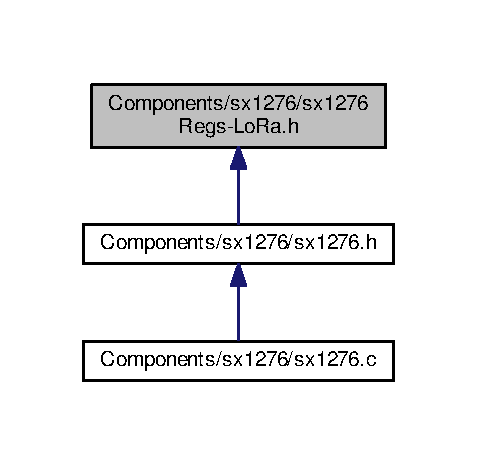
\includegraphics[width=229pt]{sx1276Regs-LoRa_8h__dep__incl}
\end{center}
\end{figure}
\subsection*{Macros}
\begin{DoxyCompactItemize}
\item 
\#define \hyperlink{sx1276Regs-LoRa_8h_a0f3e3ea7703c7cb55e2fa4c02ebc6edb}{R\+E\+G\+\_\+\+L\+R\+\_\+\+F\+I\+FO}~0x00
\item 
\#define \hyperlink{sx1276Regs-LoRa_8h_ae13863a0cab88f39c29d875010dc5b25}{R\+E\+G\+\_\+\+L\+R\+\_\+\+O\+P\+M\+O\+DE}~0x01
\item 
\#define \hyperlink{sx1276Regs-LoRa_8h_a8649d29d6156853059baf0e882ee52ec}{R\+E\+G\+\_\+\+L\+R\+\_\+\+F\+R\+F\+M\+SB}~0x06
\item 
\#define \hyperlink{sx1276Regs-LoRa_8h_a63a5c5592931ff821f237f6393b54d95}{R\+E\+G\+\_\+\+L\+R\+\_\+\+F\+R\+F\+M\+ID}~0x07
\item 
\#define \hyperlink{sx1276Regs-LoRa_8h_a97328f9a41f18eb8a0888e003104626a}{R\+E\+G\+\_\+\+L\+R\+\_\+\+F\+R\+F\+L\+SB}~0x08
\item 
\#define \hyperlink{sx1276Regs-LoRa_8h_a8dfd910a5d3e587f7772052710ac3376}{R\+E\+G\+\_\+\+L\+R\+\_\+\+P\+A\+C\+O\+N\+F\+IG}~0x09
\item 
\#define \hyperlink{sx1276Regs-LoRa_8h_a5e5599cfeecea91ca7c5ba1e68c70882}{R\+E\+G\+\_\+\+L\+R\+\_\+\+P\+A\+R\+A\+MP}~0x0A
\item 
\#define \hyperlink{sx1276Regs-LoRa_8h_acdfdcf7cfc15f16c5c8d59fee923ca5f}{R\+E\+G\+\_\+\+L\+R\+\_\+\+O\+CP}~0x0B
\item 
\#define \hyperlink{sx1276Regs-LoRa_8h_a3a52a9b28aecbdddf291c14fe1b69b68}{R\+E\+G\+\_\+\+L\+R\+\_\+\+L\+NA}~0x0C
\item 
\#define \hyperlink{sx1276Regs-LoRa_8h_abdc4c3b5c640a1069f7be689ad5bd908}{R\+E\+G\+\_\+\+L\+R\+\_\+\+F\+I\+F\+O\+A\+D\+D\+R\+P\+TR}~0x0D
\item 
\#define \hyperlink{sx1276Regs-LoRa_8h_a317be2161e52b7ae141564e19598de85}{R\+E\+G\+\_\+\+L\+R\+\_\+\+F\+I\+F\+O\+T\+X\+B\+A\+S\+E\+A\+D\+DR}~0x0E
\item 
\#define \hyperlink{sx1276Regs-LoRa_8h_ad0c1f657286b341e8a305fcc546ff391}{R\+E\+G\+\_\+\+L\+R\+\_\+\+F\+I\+F\+O\+R\+X\+B\+A\+S\+E\+A\+D\+DR}~0x0F
\item 
\#define \hyperlink{sx1276Regs-LoRa_8h_ab571f7dfb8c742a652e427b983cc6962}{R\+E\+G\+\_\+\+L\+R\+\_\+\+F\+I\+F\+O\+R\+X\+C\+U\+R\+R\+E\+N\+T\+A\+D\+DR}~0x10
\item 
\#define \hyperlink{sx1276Regs-LoRa_8h_a2b50ca91ed7db2035a2183b37506eec8}{R\+E\+G\+\_\+\+L\+R\+\_\+\+I\+R\+Q\+F\+L\+A\+G\+S\+M\+A\+SK}~0x11
\item 
\#define \hyperlink{sx1276Regs-LoRa_8h_a29222ef4f73d911623275ebbb7ddbaf0}{R\+E\+G\+\_\+\+L\+R\+\_\+\+I\+R\+Q\+F\+L\+A\+GS}~0x12
\item 
\#define \hyperlink{sx1276Regs-LoRa_8h_a5443dae2a149465cebef0aa8aad4d8aa}{R\+E\+G\+\_\+\+L\+R\+\_\+\+R\+X\+N\+B\+B\+Y\+T\+ES}~0x13
\item 
\#define \hyperlink{sx1276Regs-LoRa_8h_aaf42f47bffbc4e33e7a4a10a81aee5e7}{R\+E\+G\+\_\+\+L\+R\+\_\+\+R\+X\+H\+E\+A\+D\+E\+R\+C\+N\+T\+V\+A\+L\+U\+E\+M\+SB}~0x14
\item 
\#define \hyperlink{sx1276Regs-LoRa_8h_a8153ac7c0d03f1c769485b112383a733}{R\+E\+G\+\_\+\+L\+R\+\_\+\+R\+X\+H\+E\+A\+D\+E\+R\+C\+N\+T\+V\+A\+L\+U\+E\+L\+SB}~0x15
\item 
\#define \hyperlink{sx1276Regs-LoRa_8h_aab224430e41cf39e050a92927b8a2e03}{R\+E\+G\+\_\+\+L\+R\+\_\+\+R\+X\+P\+A\+C\+K\+E\+T\+C\+N\+T\+V\+A\+L\+U\+E\+M\+SB}~0x16
\item 
\#define \hyperlink{sx1276Regs-LoRa_8h_a999636679ece11f0f6cb0ad058db863a}{R\+E\+G\+\_\+\+L\+R\+\_\+\+R\+X\+P\+A\+C\+K\+E\+T\+C\+N\+T\+V\+A\+L\+U\+E\+L\+SB}~0x17
\item 
\#define \hyperlink{sx1276Regs-LoRa_8h_ac633e60a75224b850dc8429394e80e7c}{R\+E\+G\+\_\+\+L\+R\+\_\+\+M\+O\+D\+E\+M\+S\+T\+AT}~0x18
\item 
\#define \hyperlink{sx1276Regs-LoRa_8h_a2b0bc71a6460bd6e97cf8a6717c90cc5}{R\+E\+G\+\_\+\+L\+R\+\_\+\+P\+K\+T\+S\+N\+R\+V\+A\+L\+UE}~0x19
\item 
\#define \hyperlink{sx1276Regs-LoRa_8h_ac7db39cc10de754e5e5d7065ca2c1796}{R\+E\+G\+\_\+\+L\+R\+\_\+\+P\+K\+T\+R\+S\+S\+I\+V\+A\+L\+UE}~0x1A
\item 
\#define \hyperlink{sx1276Regs-LoRa_8h_a51636b899dd268fa04ddfa2c66329f05}{R\+E\+G\+\_\+\+L\+R\+\_\+\+R\+S\+S\+I\+V\+A\+L\+UE}~0x1B
\item 
\#define \hyperlink{sx1276Regs-LoRa_8h_a5eb22acab75323e171815532117539e4}{R\+E\+G\+\_\+\+L\+R\+\_\+\+H\+O\+P\+C\+H\+A\+N\+N\+EL}~0x1C
\item 
\#define \hyperlink{sx1276Regs-LoRa_8h_af759d830088be4284079ba8aa75d98ae}{R\+E\+G\+\_\+\+L\+R\+\_\+\+M\+O\+D\+E\+M\+C\+O\+N\+F\+I\+G1}~0x1D
\item 
\#define \hyperlink{sx1276Regs-LoRa_8h_ae96f87f817a89b1240cfdc89f17b6e30}{R\+E\+G\+\_\+\+L\+R\+\_\+\+M\+O\+D\+E\+M\+C\+O\+N\+F\+I\+G2}~0x1E
\item 
\#define \hyperlink{sx1276Regs-LoRa_8h_a7759fc860cf446c7e1a92a823a89ea31}{R\+E\+G\+\_\+\+L\+R\+\_\+\+S\+Y\+M\+B\+T\+I\+M\+E\+O\+U\+T\+L\+SB}~0x1F
\item 
\#define \hyperlink{sx1276Regs-LoRa_8h_a786457a6b4788117f8a2b994e68344ba}{R\+E\+G\+\_\+\+L\+R\+\_\+\+P\+R\+E\+A\+M\+B\+L\+E\+M\+SB}~0x20
\item 
\#define \hyperlink{sx1276Regs-LoRa_8h_a4449a1e2b055269d13034ebb4ba705b2}{R\+E\+G\+\_\+\+L\+R\+\_\+\+P\+R\+E\+A\+M\+B\+L\+E\+L\+SB}~0x21
\item 
\#define \hyperlink{sx1276Regs-LoRa_8h_a702e1e9ac301d26eb08fed50b90c6718}{R\+E\+G\+\_\+\+L\+R\+\_\+\+P\+A\+Y\+L\+O\+A\+D\+L\+E\+N\+G\+TH}~0x22
\item 
\#define \hyperlink{sx1276Regs-LoRa_8h_ae71e7acfa7c8c737e55349e72c71349f}{R\+E\+G\+\_\+\+L\+R\+\_\+\+P\+A\+Y\+L\+O\+A\+D\+M\+A\+X\+L\+E\+N\+G\+TH}~0x23
\item 
\#define \hyperlink{sx1276Regs-LoRa_8h_a829b59cc8b18d86904af96d1dc60add2}{R\+E\+G\+\_\+\+L\+R\+\_\+\+H\+O\+P\+P\+E\+R\+I\+OD}~0x24
\item 
\#define \hyperlink{sx1276Regs-LoRa_8h_a71cd184cd1fae95aeb458d8361d51cdd}{R\+E\+G\+\_\+\+L\+R\+\_\+\+F\+I\+F\+O\+R\+X\+B\+Y\+T\+E\+A\+D\+DR}~0x25
\item 
\#define \hyperlink{sx1276Regs-LoRa_8h_aecf214e63c69601e543629269b0401c7}{R\+E\+G\+\_\+\+L\+R\+\_\+\+M\+O\+D\+E\+M\+C\+O\+N\+F\+I\+G3}~0x26
\item 
\#define \hyperlink{sx1276Regs-LoRa_8h_a71a7b80d5f8a8c64cd63ea8d81a33d26}{R\+E\+G\+\_\+\+L\+R\+\_\+\+F\+E\+I\+M\+SB}~0x28
\item 
\#define \hyperlink{sx1276Regs-LoRa_8h_a300ed0b1d23a5723176cfb26dcf2b32c}{R\+E\+G\+\_\+\+L\+R\+\_\+\+F\+E\+I\+M\+ID}~0x29
\item 
\#define \hyperlink{sx1276Regs-LoRa_8h_a515106b61bc60484b381cc58afa28b6e}{R\+E\+G\+\_\+\+L\+R\+\_\+\+F\+E\+I\+L\+SB}~0x2A
\item 
\#define \hyperlink{sx1276Regs-LoRa_8h_a98748f71ec5ffb1945bf8fa7a91a5d45}{R\+E\+G\+\_\+\+L\+R\+\_\+\+R\+S\+S\+I\+W\+I\+D\+E\+B\+A\+ND}~0x2C
\item 
\#define \hyperlink{sx1276Regs-LoRa_8h_af5f1829a69cb2a95243952ffa751a4c9}{R\+E\+G\+\_\+\+L\+R\+\_\+\+T\+E\+S\+T2F}~0x2F
\item 
\#define \hyperlink{sx1276Regs-LoRa_8h_a74451ab459bd0f482dde3ee50592390b}{R\+E\+G\+\_\+\+L\+R\+\_\+\+T\+E\+S\+T30}~0x30
\item 
\#define \hyperlink{sx1276Regs-LoRa_8h_a62883b6ca8e236af4d331a31e55c67b3}{R\+E\+G\+\_\+\+L\+R\+\_\+\+D\+E\+T\+E\+C\+T\+O\+P\+T\+I\+M\+I\+ZE}~0x31
\item 
\#define \hyperlink{sx1276Regs-LoRa_8h_afc2779efc44625851e1d056f48fa1f0c}{R\+E\+G\+\_\+\+L\+R\+\_\+\+I\+N\+V\+E\+R\+T\+IQ}~0x33
\item 
\#define \hyperlink{sx1276Regs-LoRa_8h_a08173e8721d25c6ab32e8aa4c157751d}{R\+E\+G\+\_\+\+L\+R\+\_\+\+T\+E\+S\+T36}~0x36
\item 
\#define \hyperlink{sx1276Regs-LoRa_8h_abc835e71071bd5f3bd52f54168d6e4b7}{R\+E\+G\+\_\+\+L\+R\+\_\+\+D\+E\+T\+E\+C\+T\+I\+O\+N\+T\+H\+R\+E\+S\+H\+O\+LD}~0x37
\item 
\#define \hyperlink{sx1276Regs-LoRa_8h_a9da3702bd320fa729cb809d07ef0c38a}{R\+E\+G\+\_\+\+L\+R\+\_\+\+S\+Y\+N\+C\+W\+O\+RD}~0x39
\item 
\#define \hyperlink{sx1276Regs-LoRa_8h_a4dd28b78370d8732b9d149f71826e62d}{R\+E\+G\+\_\+\+L\+R\+\_\+\+T\+E\+S\+T3A}~0x3A
\item 
\#define \hyperlink{sx1276Regs-LoRa_8h_a83e2628ed2b5dcf9d0a30e7317b9a560}{R\+E\+G\+\_\+\+L\+R\+\_\+\+I\+N\+V\+E\+R\+T\+I\+Q2}~0x3B
\item 
\#define \hyperlink{sx1276Regs-LoRa_8h_a153226eac782c0908150527e844dc42f}{R\+E\+G\+\_\+\+L\+R\+\_\+\+D\+I\+O\+M\+A\+P\+P\+I\+N\+G1}~0x40
\item 
\#define \hyperlink{sx1276Regs-LoRa_8h_a13a4beabb022493d7f714e49e44e1715}{R\+E\+G\+\_\+\+L\+R\+\_\+\+D\+I\+O\+M\+A\+P\+P\+I\+N\+G2}~0x41
\item 
\#define \hyperlink{sx1276Regs-LoRa_8h_a8161394887fc1ff67af883e55afa006e}{R\+E\+G\+\_\+\+L\+R\+\_\+\+V\+E\+R\+S\+I\+ON}~0x42
\item 
\#define \hyperlink{sx1276Regs-LoRa_8h_af71d93b5478ef3e6058e3787a1095503}{R\+E\+G\+\_\+\+L\+R\+\_\+\+P\+L\+L\+H\+OP}~0x44
\item 
\#define \hyperlink{sx1276Regs-LoRa_8h_ab7ec38544ea3e38b672c3c786607b3ea}{R\+E\+G\+\_\+\+L\+R\+\_\+\+T\+C\+XO}~0x4B
\item 
\#define \hyperlink{sx1276Regs-LoRa_8h_a0fe80f278fb8bf0702faad66404d4a5c}{R\+E\+G\+\_\+\+L\+R\+\_\+\+P\+A\+D\+AC}~0x4D
\item 
\#define \hyperlink{sx1276Regs-LoRa_8h_a8eedbc42b755b17b123d3ecdb8d785b8}{R\+E\+G\+\_\+\+L\+R\+\_\+\+F\+O\+R\+M\+E\+R\+T\+E\+MP}~0x5B
\item 
\#define \hyperlink{sx1276Regs-LoRa_8h_ab2660874b741525fc0424f8b0c59fb00}{R\+E\+G\+\_\+\+L\+R\+\_\+\+B\+I\+T\+R\+A\+T\+E\+F\+R\+AC}~0x5D
\item 
\#define \hyperlink{sx1276Regs-LoRa_8h_a3ad00cd303907ff68744172e6bf219c8}{R\+E\+G\+\_\+\+L\+R\+\_\+\+A\+G\+C\+R\+EF}~0x61
\item 
\#define \hyperlink{sx1276Regs-LoRa_8h_a5b15d639723d2681ebaa2d5f31286ce5}{R\+E\+G\+\_\+\+L\+R\+\_\+\+A\+G\+C\+T\+H\+R\+E\+S\+H1}~0x62
\item 
\#define \hyperlink{sx1276Regs-LoRa_8h_a58a2478774db4cf2ff4bdc89c7f29eff}{R\+E\+G\+\_\+\+L\+R\+\_\+\+A\+G\+C\+T\+H\+R\+E\+S\+H2}~0x63
\item 
\#define \hyperlink{sx1276Regs-LoRa_8h_a546cd6aa87137c48b5c98c5973f6f8de}{R\+E\+G\+\_\+\+L\+R\+\_\+\+A\+G\+C\+T\+H\+R\+E\+S\+H3}~0x64
\item 
\#define \hyperlink{sx1276Regs-LoRa_8h_a59ec52cf30ae082fee02bdf04a95dcf8}{R\+E\+G\+\_\+\+L\+R\+\_\+\+P\+LL}~0x70
\item 
\#define \hyperlink{sx1276Regs-LoRa_8h_a4f5c6acc1ecbded1e724e4d8d4614a4d}{R\+F\+L\+R\+\_\+\+O\+P\+M\+O\+D\+E\+\_\+\+L\+O\+N\+G\+R\+A\+N\+G\+E\+M\+O\+D\+E\+\_\+\+M\+A\+SK}~0x7F
\item 
\#define \hyperlink{sx1276Regs-LoRa_8h_abb6cc4dc044295367651d11fb77508bd}{R\+F\+L\+R\+\_\+\+O\+P\+M\+O\+D\+E\+\_\+\+L\+O\+N\+G\+R\+A\+N\+G\+E\+M\+O\+D\+E\+\_\+\+O\+FF}~0x00
\item 
\#define \hyperlink{sx1276Regs-LoRa_8h_a4d9b59767f3e421ed4b6a5857c1007bf}{R\+F\+L\+R\+\_\+\+O\+P\+M\+O\+D\+E\+\_\+\+L\+O\+N\+G\+R\+A\+N\+G\+E\+M\+O\+D\+E\+\_\+\+ON}~0x80
\item 
\#define \hyperlink{sx1276Regs-LoRa_8h_a01598cd825d7b0a773e420ba4811067c}{R\+F\+L\+R\+\_\+\+O\+P\+M\+O\+D\+E\+\_\+\+A\+C\+C\+E\+S\+S\+S\+H\+A\+R\+E\+D\+R\+E\+G\+\_\+\+M\+A\+SK}~0x\+BF
\item 
\#define \hyperlink{sx1276Regs-LoRa_8h_a32305e7842ed6a5e27dea62504bb59da}{R\+F\+L\+R\+\_\+\+O\+P\+M\+O\+D\+E\+\_\+\+A\+C\+C\+E\+S\+S\+S\+H\+A\+R\+E\+D\+R\+E\+G\+\_\+\+E\+N\+A\+B\+LE}~0x40
\item 
\#define \hyperlink{sx1276Regs-LoRa_8h_ad9b5fa39ecfbad14292001a38b5db44d}{R\+F\+L\+R\+\_\+\+O\+P\+M\+O\+D\+E\+\_\+\+A\+C\+C\+E\+S\+S\+S\+H\+A\+R\+E\+D\+R\+E\+G\+\_\+\+D\+I\+S\+A\+B\+LE}~0x00
\item 
\#define \hyperlink{sx1276Regs-LoRa_8h_af78146c81e7e2c1d15a3c1f487fc8237}{R\+F\+L\+R\+\_\+\+O\+P\+M\+O\+D\+E\+\_\+\+F\+R\+E\+Q\+M\+O\+D\+E\+\_\+\+A\+C\+C\+E\+S\+S\+\_\+\+M\+A\+SK}~0x\+F7
\item 
\#define \hyperlink{sx1276Regs-LoRa_8h_ac3b485df85439dc57b6ff9fa4b4e7178}{R\+F\+L\+R\+\_\+\+O\+P\+M\+O\+D\+E\+\_\+\+F\+R\+E\+Q\+M\+O\+D\+E\+\_\+\+A\+C\+C\+E\+S\+S\+\_\+\+LF}~0x08
\item 
\#define \hyperlink{sx1276Regs-LoRa_8h_aa8585403cacfc764a79455a2e82507bf}{R\+F\+L\+R\+\_\+\+O\+P\+M\+O\+D\+E\+\_\+\+F\+R\+E\+Q\+M\+O\+D\+E\+\_\+\+A\+C\+C\+E\+S\+S\+\_\+\+HF}~0x00
\item 
\#define \hyperlink{sx1276Regs-LoRa_8h_ae81262dc31f1b6843d2d09125dda0659}{R\+F\+L\+R\+\_\+\+O\+P\+M\+O\+D\+E\+\_\+\+M\+A\+SK}~0x\+F8
\item 
\#define \hyperlink{sx1276Regs-LoRa_8h_a042c25d6f974d449c3ba24782751cd45}{R\+F\+L\+R\+\_\+\+O\+P\+M\+O\+D\+E\+\_\+\+S\+L\+E\+EP}~0x00
\item 
\#define \hyperlink{sx1276Regs-LoRa_8h_afb7498d406642d2e07cb383010697c0a}{R\+F\+L\+R\+\_\+\+O\+P\+M\+O\+D\+E\+\_\+\+S\+T\+A\+N\+D\+BY}~0x01
\item 
\#define \hyperlink{sx1276Regs-LoRa_8h_ab5c2916d7198480084d9275020ed67f0}{R\+F\+L\+R\+\_\+\+O\+P\+M\+O\+D\+E\+\_\+\+S\+Y\+N\+T\+H\+E\+S\+I\+Z\+E\+R\+\_\+\+TX}~0x02
\item 
\#define \hyperlink{sx1276Regs-LoRa_8h_a2ccdd26a6b1283c6f8f0710b49269d02}{R\+F\+L\+R\+\_\+\+O\+P\+M\+O\+D\+E\+\_\+\+T\+R\+A\+N\+S\+M\+I\+T\+T\+ER}~0x03
\item 
\#define \hyperlink{sx1276Regs-LoRa_8h_a51b6a8bcd4bb5e0016428956ffa91794}{R\+F\+L\+R\+\_\+\+O\+P\+M\+O\+D\+E\+\_\+\+S\+Y\+N\+T\+H\+E\+S\+I\+Z\+E\+R\+\_\+\+RX}~0x04
\item 
\#define \hyperlink{sx1276Regs-LoRa_8h_a18ffa4e2930797bbeb71fd15ae77dfe0}{R\+F\+L\+R\+\_\+\+O\+P\+M\+O\+D\+E\+\_\+\+R\+E\+C\+E\+I\+V\+ER}~0x05
\item 
\#define \hyperlink{sx1276Regs-LoRa_8h_a0cfa7959ea68f8e81d1ee04e8a3ef596}{R\+F\+L\+R\+\_\+\+O\+P\+M\+O\+D\+E\+\_\+\+R\+E\+C\+E\+I\+V\+E\+R\+\_\+\+S\+I\+N\+G\+LE}~0x06
\item 
\#define \hyperlink{sx1276Regs-LoRa_8h_a8e3c7ec4d0aceedae1069a3b6d8d6bd2}{R\+F\+L\+R\+\_\+\+O\+P\+M\+O\+D\+E\+\_\+\+C\+AD}~0x07
\item 
\#define \hyperlink{sx1276Regs-LoRa_8h_ac8e626a7d3028cc58dbe937ce2cb4fef}{R\+F\+L\+R\+\_\+\+F\+R\+F\+M\+S\+B\+\_\+434\+\_\+\+M\+HZ}~0x6C
\item 
\#define \hyperlink{sx1276Regs-LoRa_8h_a2b6e1709a469a8e5fe8c3099036576b2}{R\+F\+L\+R\+\_\+\+F\+R\+F\+M\+I\+D\+\_\+434\+\_\+\+M\+HZ}~0x80
\item 
\#define \hyperlink{sx1276Regs-LoRa_8h_a9fbeb4068d680304497804b2e3b01cc1}{R\+F\+L\+R\+\_\+\+F\+R\+F\+L\+S\+B\+\_\+434\+\_\+\+M\+HZ}~0x00
\item 
\#define \hyperlink{sx1276Regs-LoRa_8h_a98fc674afce865acf9efb9a1c2ab39a3}{R\+F\+L\+R\+\_\+\+P\+A\+C\+O\+N\+F\+I\+G\+\_\+\+P\+A\+S\+E\+L\+E\+C\+T\+\_\+\+M\+A\+SK}~0x7F
\item 
\#define \hyperlink{sx1276Regs-LoRa_8h_a268b1d9d7fa806038150cabff6dee9a7}{R\+F\+L\+R\+\_\+\+P\+A\+C\+O\+N\+F\+I\+G\+\_\+\+P\+A\+S\+E\+L\+E\+C\+T\+\_\+\+P\+A\+B\+O\+O\+ST}~0x80
\item 
\#define \hyperlink{sx1276Regs-LoRa_8h_a584857e70a2e6fddfb11bc51775b35a6}{R\+F\+L\+R\+\_\+\+P\+A\+C\+O\+N\+F\+I\+G\+\_\+\+P\+A\+S\+E\+L\+E\+C\+T\+\_\+\+R\+FO}~0x00
\item 
\#define \hyperlink{sx1276Regs-LoRa_8h_a2045361d9d317c305aed6e405420ab81}{R\+F\+L\+R\+\_\+\+P\+A\+C\+O\+N\+F\+I\+G\+\_\+\+M\+A\+X\+\_\+\+P\+O\+W\+E\+R\+\_\+\+M\+A\+SK}~0x8F
\item 
\#define \hyperlink{sx1276Regs-LoRa_8h_a1d4448a184c398c43e06bfad5102730f}{R\+F\+L\+R\+\_\+\+P\+A\+C\+O\+N\+F\+I\+G\+\_\+\+O\+U\+T\+P\+U\+T\+P\+O\+W\+E\+R\+\_\+\+M\+A\+SK}~0x\+F0
\item 
\#define \hyperlink{sx1276Regs-LoRa_8h_a9112c35a5e33d45453157d1a04591294}{R\+F\+L\+R\+\_\+\+P\+A\+R\+A\+M\+P\+\_\+\+T\+X\+B\+A\+N\+D\+F\+O\+R\+C\+E\+\_\+\+M\+A\+SK}~0x\+EF
\item 
\#define \hyperlink{sx1276Regs-LoRa_8h_ad45572b9fe781c4e783cc7aef19b1406}{R\+F\+L\+R\+\_\+\+P\+A\+R\+A\+M\+P\+\_\+\+T\+X\+B\+A\+N\+D\+F\+O\+R\+C\+E\+\_\+\+B\+A\+N\+D\+\_\+\+S\+EL}~0x10
\item 
\#define \hyperlink{sx1276Regs-LoRa_8h_aeaf1429172c5196bcaa7f5d3079113d1}{R\+F\+L\+R\+\_\+\+P\+A\+R\+A\+M\+P\+\_\+\+T\+X\+B\+A\+N\+D\+F\+O\+R\+C\+E\+\_\+\+A\+U\+TO}~0x00
\item 
\#define \hyperlink{sx1276Regs-LoRa_8h_a8e2df5205bbee456190800ae3e6c5b48}{R\+F\+L\+R\+\_\+\+P\+A\+R\+A\+M\+P\+\_\+\+M\+A\+SK}~0x\+F0
\item 
\#define \hyperlink{sx1276Regs-LoRa_8h_a17650ac6f6503f25d99fc36183d339fb}{R\+F\+L\+R\+\_\+\+P\+A\+R\+A\+M\+P\+\_\+3400\+\_\+\+US}~0x00
\item 
\#define \hyperlink{sx1276Regs-LoRa_8h_a54e4bb780307ff67f9319190a061ed65}{R\+F\+L\+R\+\_\+\+P\+A\+R\+A\+M\+P\+\_\+2000\+\_\+\+US}~0x01
\item 
\#define \hyperlink{sx1276Regs-LoRa_8h_aa50dc8d791c24398ad463dbbe163c218}{R\+F\+L\+R\+\_\+\+P\+A\+R\+A\+M\+P\+\_\+1000\+\_\+\+US}~0x02
\item 
\#define \hyperlink{sx1276Regs-LoRa_8h_a268b294289d89cac69a2f50608292fb9}{R\+F\+L\+R\+\_\+\+P\+A\+R\+A\+M\+P\+\_\+0500\+\_\+\+US}~0x03
\item 
\#define \hyperlink{sx1276Regs-LoRa_8h_a31b242b14f8b2b7fb9bf6a0634fe43e2}{R\+F\+L\+R\+\_\+\+P\+A\+R\+A\+M\+P\+\_\+0250\+\_\+\+US}~0x04
\item 
\#define \hyperlink{sx1276Regs-LoRa_8h_a2ae8ceffd161e8c509cc076715b71c15}{R\+F\+L\+R\+\_\+\+P\+A\+R\+A\+M\+P\+\_\+0125\+\_\+\+US}~0x05
\item 
\#define \hyperlink{sx1276Regs-LoRa_8h_a23f0326e72ee3f1041d32f7edbe30733}{R\+F\+L\+R\+\_\+\+P\+A\+R\+A\+M\+P\+\_\+0100\+\_\+\+US}~0x06
\item 
\#define \hyperlink{sx1276Regs-LoRa_8h_a274b21f651fded0ec4d35ed18dc281da}{R\+F\+L\+R\+\_\+\+P\+A\+R\+A\+M\+P\+\_\+0062\+\_\+\+US}~0x07
\item 
\#define \hyperlink{sx1276Regs-LoRa_8h_a00d7b1b7436424f43314df712aa89fe2}{R\+F\+L\+R\+\_\+\+P\+A\+R\+A\+M\+P\+\_\+0050\+\_\+\+US}~0x08
\item 
\#define \hyperlink{sx1276Regs-LoRa_8h_a9ce8032bc528b8f1a56e72a0fe6fb956}{R\+F\+L\+R\+\_\+\+P\+A\+R\+A\+M\+P\+\_\+0040\+\_\+\+US}~0x09
\item 
\#define \hyperlink{sx1276Regs-LoRa_8h_ae596e916faaf110c1306996dbd93d25f}{R\+F\+L\+R\+\_\+\+P\+A\+R\+A\+M\+P\+\_\+0031\+\_\+\+US}~0x0A
\item 
\#define \hyperlink{sx1276Regs-LoRa_8h_adb4da3360a1b4adf5de2c99f86d502c7}{R\+F\+L\+R\+\_\+\+P\+A\+R\+A\+M\+P\+\_\+0025\+\_\+\+US}~0x0B
\item 
\#define \hyperlink{sx1276Regs-LoRa_8h_afd5af86b9fcd58b5da08d807ab0deae5}{R\+F\+L\+R\+\_\+\+P\+A\+R\+A\+M\+P\+\_\+0020\+\_\+\+US}~0x0C
\item 
\#define \hyperlink{sx1276Regs-LoRa_8h_a58992d8a87351616671bb667124c136a}{R\+F\+L\+R\+\_\+\+P\+A\+R\+A\+M\+P\+\_\+0015\+\_\+\+US}~0x0D
\item 
\#define \hyperlink{sx1276Regs-LoRa_8h_a6af078a4ad16e7e83d180c4470e174e1}{R\+F\+L\+R\+\_\+\+P\+A\+R\+A\+M\+P\+\_\+0012\+\_\+\+US}~0x0E
\item 
\#define \hyperlink{sx1276Regs-LoRa_8h_a42510cd3823fa579f7ce0a2590414d94}{R\+F\+L\+R\+\_\+\+P\+A\+R\+A\+M\+P\+\_\+0010\+\_\+\+US}~0x0F
\item 
\#define \hyperlink{sx1276Regs-LoRa_8h_a811d1ea4838fb5bdbc731e246f9abd00}{R\+F\+L\+R\+\_\+\+O\+C\+P\+\_\+\+M\+A\+SK}~0x\+DF
\item 
\#define \hyperlink{sx1276Regs-LoRa_8h_ab4cd8bafefd94bf96c0eda92a1a0e2cc}{R\+F\+L\+R\+\_\+\+O\+C\+P\+\_\+\+ON}~0x20
\item 
\#define \hyperlink{sx1276Regs-LoRa_8h_add262ca41df12a73f7ab0fe05ca26253}{R\+F\+L\+R\+\_\+\+O\+C\+P\+\_\+\+O\+FF}~0x00
\item 
\#define \hyperlink{sx1276Regs-LoRa_8h_a218c5b62787ba2141067b6273f2e43a3}{R\+F\+L\+R\+\_\+\+O\+C\+P\+\_\+\+T\+R\+I\+M\+\_\+\+M\+A\+SK}~0x\+E0
\item 
\#define \hyperlink{sx1276Regs-LoRa_8h_a6656289f06f654d070ee51d72830d1cb}{R\+F\+L\+R\+\_\+\+O\+C\+P\+\_\+\+T\+R\+I\+M\+\_\+045\+\_\+\+MA}~0x00
\item 
\#define \hyperlink{sx1276Regs-LoRa_8h_a102d3235b329da485a39882b6f06fec4}{R\+F\+L\+R\+\_\+\+O\+C\+P\+\_\+\+T\+R\+I\+M\+\_\+050\+\_\+\+MA}~0x01
\item 
\#define \hyperlink{sx1276Regs-LoRa_8h_a916a524ad394506a119ea2c5d8d2642c}{R\+F\+L\+R\+\_\+\+O\+C\+P\+\_\+\+T\+R\+I\+M\+\_\+055\+\_\+\+MA}~0x02
\item 
\#define \hyperlink{sx1276Regs-LoRa_8h_a7fc3cb1a990f3c479cf620772593991b}{R\+F\+L\+R\+\_\+\+O\+C\+P\+\_\+\+T\+R\+I\+M\+\_\+060\+\_\+\+MA}~0x03
\item 
\#define \hyperlink{sx1276Regs-LoRa_8h_a1d7e9642b9adfb481f9696186a068db8}{R\+F\+L\+R\+\_\+\+O\+C\+P\+\_\+\+T\+R\+I\+M\+\_\+065\+\_\+\+MA}~0x04
\item 
\#define \hyperlink{sx1276Regs-LoRa_8h_a08ffd9de8d0ea7320df82bf3ddd38430}{R\+F\+L\+R\+\_\+\+O\+C\+P\+\_\+\+T\+R\+I\+M\+\_\+070\+\_\+\+MA}~0x05
\item 
\#define \hyperlink{sx1276Regs-LoRa_8h_add96158d00533ceefc7b0ab356e4a6cc}{R\+F\+L\+R\+\_\+\+O\+C\+P\+\_\+\+T\+R\+I\+M\+\_\+075\+\_\+\+MA}~0x06
\item 
\#define \hyperlink{sx1276Regs-LoRa_8h_a2551f7eacef1961881b7b38c724b393b}{R\+F\+L\+R\+\_\+\+O\+C\+P\+\_\+\+T\+R\+I\+M\+\_\+080\+\_\+\+MA}~0x07
\item 
\#define \hyperlink{sx1276Regs-LoRa_8h_a944d696fcf109d939378d53b4f85f9fb}{R\+F\+L\+R\+\_\+\+O\+C\+P\+\_\+\+T\+R\+I\+M\+\_\+085\+\_\+\+MA}~0x08
\item 
\#define \hyperlink{sx1276Regs-LoRa_8h_a4928b1121ada662258df2b1741f8f6ea}{R\+F\+L\+R\+\_\+\+O\+C\+P\+\_\+\+T\+R\+I\+M\+\_\+090\+\_\+\+MA}~0x09
\item 
\#define \hyperlink{sx1276Regs-LoRa_8h_a701a4cf9ac291205389f408f2a37755b}{R\+F\+L\+R\+\_\+\+O\+C\+P\+\_\+\+T\+R\+I\+M\+\_\+095\+\_\+\+MA}~0x0A
\item 
\#define \hyperlink{sx1276Regs-LoRa_8h_a9dde9ac43efb12556edd486e76ceec63}{R\+F\+L\+R\+\_\+\+O\+C\+P\+\_\+\+T\+R\+I\+M\+\_\+100\+\_\+\+MA}~0x0B
\item 
\#define \hyperlink{sx1276Regs-LoRa_8h_afe5f0e6dfa00877d42470d27df2cf3ad}{R\+F\+L\+R\+\_\+\+O\+C\+P\+\_\+\+T\+R\+I\+M\+\_\+105\+\_\+\+MA}~0x0C
\item 
\#define \hyperlink{sx1276Regs-LoRa_8h_a8e37fe5976b5ec9bc44a3b2af08924b6}{R\+F\+L\+R\+\_\+\+O\+C\+P\+\_\+\+T\+R\+I\+M\+\_\+110\+\_\+\+MA}~0x0D
\item 
\#define \hyperlink{sx1276Regs-LoRa_8h_afaa7abafc08d83bcb214bf99ca93ee7c}{R\+F\+L\+R\+\_\+\+O\+C\+P\+\_\+\+T\+R\+I\+M\+\_\+115\+\_\+\+MA}~0x0E
\item 
\#define \hyperlink{sx1276Regs-LoRa_8h_aab5037b9ac3e1bc7e2eedccf9193ba28}{R\+F\+L\+R\+\_\+\+O\+C\+P\+\_\+\+T\+R\+I\+M\+\_\+120\+\_\+\+MA}~0x0F
\item 
\#define \hyperlink{sx1276Regs-LoRa_8h_a883d12dc95ff98fb03fc31ce6ddc2811}{R\+F\+L\+R\+\_\+\+O\+C\+P\+\_\+\+T\+R\+I\+M\+\_\+130\+\_\+\+MA}~0x10
\item 
\#define \hyperlink{sx1276Regs-LoRa_8h_a6a2eac9941486d2997adb00c19f49d98}{R\+F\+L\+R\+\_\+\+O\+C\+P\+\_\+\+T\+R\+I\+M\+\_\+140\+\_\+\+MA}~0x11
\item 
\#define \hyperlink{sx1276Regs-LoRa_8h_af9d84c5fa6e8da9a6e9cf68ebe748a18}{R\+F\+L\+R\+\_\+\+O\+C\+P\+\_\+\+T\+R\+I\+M\+\_\+150\+\_\+\+MA}~0x12
\item 
\#define \hyperlink{sx1276Regs-LoRa_8h_a3755351c3f7f7842a523b6e7627545fe}{R\+F\+L\+R\+\_\+\+O\+C\+P\+\_\+\+T\+R\+I\+M\+\_\+160\+\_\+\+MA}~0x13
\item 
\#define \hyperlink{sx1276Regs-LoRa_8h_a13dba4245f8c69fe3dee74ebeaad4ed3}{R\+F\+L\+R\+\_\+\+O\+C\+P\+\_\+\+T\+R\+I\+M\+\_\+170\+\_\+\+MA}~0x14
\item 
\#define \hyperlink{sx1276Regs-LoRa_8h_a58209162f626269790dcb91f81340f9d}{R\+F\+L\+R\+\_\+\+O\+C\+P\+\_\+\+T\+R\+I\+M\+\_\+180\+\_\+\+MA}~0x15
\item 
\#define \hyperlink{sx1276Regs-LoRa_8h_a27d3cfb3df1cbf0d08af0ba9e57aae49}{R\+F\+L\+R\+\_\+\+O\+C\+P\+\_\+\+T\+R\+I\+M\+\_\+190\+\_\+\+MA}~0x16
\item 
\#define \hyperlink{sx1276Regs-LoRa_8h_a1979c11cd7ce8b54355954a9e0139de6}{R\+F\+L\+R\+\_\+\+O\+C\+P\+\_\+\+T\+R\+I\+M\+\_\+200\+\_\+\+MA}~0x17
\item 
\#define \hyperlink{sx1276Regs-LoRa_8h_a67bf750125a9cf6cc4137361236ad814}{R\+F\+L\+R\+\_\+\+O\+C\+P\+\_\+\+T\+R\+I\+M\+\_\+210\+\_\+\+MA}~0x18
\item 
\#define \hyperlink{sx1276Regs-LoRa_8h_a3c729a06b76ddb3b25279ab9ec9759bf}{R\+F\+L\+R\+\_\+\+O\+C\+P\+\_\+\+T\+R\+I\+M\+\_\+220\+\_\+\+MA}~0x19
\item 
\#define \hyperlink{sx1276Regs-LoRa_8h_a62fbdb1632a9ef8e2464a411ba6270ac}{R\+F\+L\+R\+\_\+\+O\+C\+P\+\_\+\+T\+R\+I\+M\+\_\+230\+\_\+\+MA}~0x1A
\item 
\#define \hyperlink{sx1276Regs-LoRa_8h_a5b9df1b8ef5dd642212f2da58fff03e3}{R\+F\+L\+R\+\_\+\+O\+C\+P\+\_\+\+T\+R\+I\+M\+\_\+240\+\_\+\+MA}~0x1B
\item 
\#define \hyperlink{sx1276Regs-LoRa_8h_adaf87cfb5bc1842f215a8905466c7c09}{R\+F\+L\+R\+\_\+\+L\+N\+A\+\_\+\+G\+A\+I\+N\+\_\+\+M\+A\+SK}~0x1F
\item 
\#define \hyperlink{sx1276Regs-LoRa_8h_a037aede58520e0ac15f5b63e9edef4fb}{R\+F\+L\+R\+\_\+\+L\+N\+A\+\_\+\+G\+A\+I\+N\+\_\+\+G1}~0x20
\item 
\#define \hyperlink{sx1276Regs-LoRa_8h_a20befb067e09b6a2f3768e8f0da43eec}{R\+F\+L\+R\+\_\+\+L\+N\+A\+\_\+\+G\+A\+I\+N\+\_\+\+G2}~0x40
\item 
\#define \hyperlink{sx1276Regs-LoRa_8h_accae2f3f70ca282fd61cb09a667901ba}{R\+F\+L\+R\+\_\+\+L\+N\+A\+\_\+\+G\+A\+I\+N\+\_\+\+G3}~0x60
\item 
\#define \hyperlink{sx1276Regs-LoRa_8h_a6d72851174c6d7664136736589055129}{R\+F\+L\+R\+\_\+\+L\+N\+A\+\_\+\+G\+A\+I\+N\+\_\+\+G4}~0x80
\item 
\#define \hyperlink{sx1276Regs-LoRa_8h_ae5719825fa402e40336c7acac639c5db}{R\+F\+L\+R\+\_\+\+L\+N\+A\+\_\+\+G\+A\+I\+N\+\_\+\+G5}~0x\+A0
\item 
\#define \hyperlink{sx1276Regs-LoRa_8h_aa16933aa89f284c5c3e9c3700d717902}{R\+F\+L\+R\+\_\+\+L\+N\+A\+\_\+\+G\+A\+I\+N\+\_\+\+G6}~0x\+C0
\item 
\#define \hyperlink{sx1276Regs-LoRa_8h_ace13d78a7979a589c7b3918412bb7140}{R\+F\+L\+R\+\_\+\+L\+N\+A\+\_\+\+B\+O\+O\+S\+T\+\_\+\+L\+F\+\_\+\+M\+A\+SK}~0x\+E7
\item 
\#define \hyperlink{sx1276Regs-LoRa_8h_a952b2dd390b6b2faff709e9950c7bdbf}{R\+F\+L\+R\+\_\+\+L\+N\+A\+\_\+\+B\+O\+O\+S\+T\+\_\+\+L\+F\+\_\+\+D\+E\+F\+A\+U\+LT}~0x00
\item 
\#define \hyperlink{sx1276Regs-LoRa_8h_a0276e7bb160dc7aeb54faf11570caee6}{R\+F\+L\+R\+\_\+\+L\+N\+A\+\_\+\+B\+O\+O\+S\+T\+\_\+\+H\+F\+\_\+\+M\+A\+SK}~0x\+FC
\item 
\#define \hyperlink{sx1276Regs-LoRa_8h_ab97ab7086b3dd953fa82bcf76347f433}{R\+F\+L\+R\+\_\+\+L\+N\+A\+\_\+\+B\+O\+O\+S\+T\+\_\+\+H\+F\+\_\+\+O\+FF}~0x00
\item 
\#define \hyperlink{sx1276Regs-LoRa_8h_af8786c60c42323ea89f1c133e9d82c43}{R\+F\+L\+R\+\_\+\+L\+N\+A\+\_\+\+B\+O\+O\+S\+T\+\_\+\+H\+F\+\_\+\+ON}~0x03
\item 
\#define \hyperlink{sx1276Regs-LoRa_8h_a293258103cd0271149fc3ddbc2eb37a2}{R\+F\+L\+R\+\_\+\+F\+I\+F\+O\+A\+D\+D\+R\+P\+TR}~0x00
\item 
\#define \hyperlink{sx1276Regs-LoRa_8h_ace89be0e3d72b0aa238de31aa1840fd3}{R\+F\+L\+R\+\_\+\+F\+I\+F\+O\+T\+X\+B\+A\+S\+E\+A\+D\+DR}~0x80
\item 
\#define \hyperlink{sx1276Regs-LoRa_8h_af2f960ed320739991501681945e45b7e}{R\+F\+L\+R\+\_\+\+F\+I\+F\+O\+R\+X\+B\+A\+S\+E\+A\+D\+DR}~0x00
\item 
\#define \hyperlink{sx1276Regs-LoRa_8h_ab60607459cabba892de2c685a14786ff}{R\+F\+L\+R\+\_\+\+I\+R\+Q\+F\+L\+A\+G\+S\+\_\+\+R\+X\+T\+I\+M\+E\+O\+U\+T\+\_\+\+M\+A\+SK}~0x80
\item 
\#define \hyperlink{sx1276Regs-LoRa_8h_aaed938b05c39afb8a66f7abc7bd31a9e}{R\+F\+L\+R\+\_\+\+I\+R\+Q\+F\+L\+A\+G\+S\+\_\+\+R\+X\+D\+O\+N\+E\+\_\+\+M\+A\+SK}~0x40
\item 
\#define \hyperlink{sx1276Regs-LoRa_8h_a4e2618c340d93f8bfd19f8634f7a63b3}{R\+F\+L\+R\+\_\+\+I\+R\+Q\+F\+L\+A\+G\+S\+\_\+\+P\+A\+Y\+L\+O\+A\+D\+C\+R\+C\+E\+R\+R\+O\+R\+\_\+\+M\+A\+SK}~0x20
\item 
\#define \hyperlink{sx1276Regs-LoRa_8h_a7d3583b774d3514d985a6f8acb6cd7c7}{R\+F\+L\+R\+\_\+\+I\+R\+Q\+F\+L\+A\+G\+S\+\_\+\+V\+A\+L\+I\+D\+H\+E\+A\+D\+E\+R\+\_\+\+M\+A\+SK}~0x10
\item 
\#define \hyperlink{sx1276Regs-LoRa_8h_adeb3e1c7ad35e4b4ab4ea7cd9050c2e6}{R\+F\+L\+R\+\_\+\+I\+R\+Q\+F\+L\+A\+G\+S\+\_\+\+T\+X\+D\+O\+N\+E\+\_\+\+M\+A\+SK}~0x08
\item 
\#define \hyperlink{sx1276Regs-LoRa_8h_a5af8031790e4a1d7c3703fb4f834b21d}{R\+F\+L\+R\+\_\+\+I\+R\+Q\+F\+L\+A\+G\+S\+\_\+\+C\+A\+D\+D\+O\+N\+E\+\_\+\+M\+A\+SK}~0x04
\item 
\#define \hyperlink{sx1276Regs-LoRa_8h_ae0250cb5809f0702a43eb235823acc44}{R\+F\+L\+R\+\_\+\+I\+R\+Q\+F\+L\+A\+G\+S\+\_\+\+F\+H\+S\+S\+C\+H\+A\+N\+G\+E\+D\+C\+H\+A\+N\+N\+E\+L\+\_\+\+M\+A\+SK}~0x02
\item 
\#define \hyperlink{sx1276Regs-LoRa_8h_a0d8e41b65bd4af8f19dfad50b7dcad97}{R\+F\+L\+R\+\_\+\+I\+R\+Q\+F\+L\+A\+G\+S\+\_\+\+C\+A\+D\+D\+E\+T\+E\+C\+T\+E\+D\+\_\+\+M\+A\+SK}~0x01
\item 
\#define \hyperlink{sx1276Regs-LoRa_8h_a12d5b2ce439396e7033053c929b815bf}{R\+F\+L\+R\+\_\+\+I\+R\+Q\+F\+L\+A\+G\+S\+\_\+\+R\+X\+T\+I\+M\+E\+O\+UT}~0x80
\item 
\#define \hyperlink{sx1276Regs-LoRa_8h_a7bdc1e0f642b272cef8fc3f81ab8d95e}{R\+F\+L\+R\+\_\+\+I\+R\+Q\+F\+L\+A\+G\+S\+\_\+\+R\+X\+D\+O\+NE}~0x40
\item 
\#define \hyperlink{sx1276Regs-LoRa_8h_a2b91f96d488f7d08d8fd543a7a5eb76b}{R\+F\+L\+R\+\_\+\+I\+R\+Q\+F\+L\+A\+G\+S\+\_\+\+P\+A\+Y\+L\+O\+A\+D\+C\+R\+C\+E\+R\+R\+OR}~0x20
\item 
\#define \hyperlink{sx1276Regs-LoRa_8h_a56f64bf676430c4ce2cc672d3bfde2b8}{R\+F\+L\+R\+\_\+\+I\+R\+Q\+F\+L\+A\+G\+S\+\_\+\+V\+A\+L\+I\+D\+H\+E\+A\+D\+ER}~0x10
\item 
\#define \hyperlink{sx1276Regs-LoRa_8h_a15a27d43d8ec6b82bcd31857c35e9f09}{R\+F\+L\+R\+\_\+\+I\+R\+Q\+F\+L\+A\+G\+S\+\_\+\+T\+X\+D\+O\+NE}~0x08
\item 
\#define \hyperlink{sx1276Regs-LoRa_8h_a44fee83993ca42bbd77370fc82c2fc91}{R\+F\+L\+R\+\_\+\+I\+R\+Q\+F\+L\+A\+G\+S\+\_\+\+C\+A\+D\+D\+O\+NE}~0x04
\item 
\#define \hyperlink{sx1276Regs-LoRa_8h_a781c17401f3c0f94e56cd76d43ca0271}{R\+F\+L\+R\+\_\+\+I\+R\+Q\+F\+L\+A\+G\+S\+\_\+\+F\+H\+S\+S\+C\+H\+A\+N\+G\+E\+D\+C\+H\+A\+N\+N\+EL}~0x02
\item 
\#define \hyperlink{sx1276Regs-LoRa_8h_a301a9870f807e6c4f54ad608da0549ed}{R\+F\+L\+R\+\_\+\+I\+R\+Q\+F\+L\+A\+G\+S\+\_\+\+C\+A\+D\+D\+E\+T\+E\+C\+T\+ED}~0x01
\item 
\#define \hyperlink{sx1276Regs-LoRa_8h_af3688cb4f2ac1d6fe5669af690e813ed}{R\+F\+L\+R\+\_\+\+M\+O\+D\+E\+M\+S\+T\+A\+T\+\_\+\+R\+X\+\_\+\+C\+R\+\_\+\+M\+A\+SK}~0x1F
\item 
\#define \hyperlink{sx1276Regs-LoRa_8h_af57dfdb07c9b3873afb53a91443b0565}{R\+F\+L\+R\+\_\+\+M\+O\+D\+E\+M\+S\+T\+A\+T\+\_\+\+M\+O\+D\+E\+M\+\_\+\+S\+T\+A\+T\+U\+S\+\_\+\+M\+A\+SK}~0x\+E0
\item 
\#define \hyperlink{sx1276Regs-LoRa_8h_a9b65f0f8d357147986b31a6c668868fb}{R\+F\+L\+R\+\_\+\+H\+O\+P\+C\+H\+A\+N\+N\+E\+L\+\_\+\+P\+L\+L\+\_\+\+L\+O\+C\+K\+\_\+\+T\+I\+M\+E\+O\+U\+T\+\_\+\+M\+A\+SK}~0x7F
\item 
\#define \hyperlink{sx1276Regs-LoRa_8h_a5585b4aec7b248eb33ae15ba12b6d91a}{R\+F\+L\+R\+\_\+\+H\+O\+P\+C\+H\+A\+N\+N\+E\+L\+\_\+\+P\+L\+L\+\_\+\+L\+O\+C\+K\+\_\+\+F\+A\+IL}~0x80
\item 
\#define \hyperlink{sx1276Regs-LoRa_8h_aee5274333f27229f37276e92627fe9d0}{R\+F\+L\+R\+\_\+\+H\+O\+P\+C\+H\+A\+N\+N\+E\+L\+\_\+\+P\+L\+L\+\_\+\+L\+O\+C\+K\+\_\+\+S\+U\+C\+C\+E\+ED}~0x00
\item 
\#define \hyperlink{sx1276Regs-LoRa_8h_aa8fbfece67ad9c1feabed0dc5018d1fa}{R\+F\+L\+R\+\_\+\+H\+O\+P\+C\+H\+A\+N\+N\+E\+L\+\_\+\+C\+R\+C\+O\+N\+P\+A\+Y\+L\+O\+A\+D\+\_\+\+M\+A\+SK}~0x\+BF
\item 
\#define \hyperlink{sx1276Regs-LoRa_8h_ab93bd7b9eac440324cb3e24bd123af06}{R\+F\+L\+R\+\_\+\+H\+O\+P\+C\+H\+A\+N\+N\+E\+L\+\_\+\+C\+R\+C\+O\+N\+P\+A\+Y\+L\+O\+A\+D\+\_\+\+ON}~0x40
\item 
\#define \hyperlink{sx1276Regs-LoRa_8h_a1355316824e22da44242051ef2e802cd}{R\+F\+L\+R\+\_\+\+H\+O\+P\+C\+H\+A\+N\+N\+E\+L\+\_\+\+C\+R\+C\+O\+N\+P\+A\+Y\+L\+O\+A\+D\+\_\+\+O\+FF}~0x00
\item 
\#define \hyperlink{sx1276Regs-LoRa_8h_a8f0d9adf82ac36ad0e801b0ab96439a2}{R\+F\+L\+R\+\_\+\+H\+O\+P\+C\+H\+A\+N\+N\+E\+L\+\_\+\+C\+H\+A\+N\+N\+E\+L\+\_\+\+M\+A\+SK}~0x3F
\item 
\#define \hyperlink{sx1276Regs-LoRa_8h_ab1aa24187e882f0f54896b50ccae77d4}{R\+F\+L\+R\+\_\+\+M\+O\+D\+E\+M\+C\+O\+N\+F\+I\+G1\+\_\+\+B\+W\+\_\+\+M\+A\+SK}~0x0F
\item 
\#define \hyperlink{sx1276Regs-LoRa_8h_a5588d7dec546c6f6f676ab4f7574604a}{R\+F\+L\+R\+\_\+\+M\+O\+D\+E\+M\+C\+O\+N\+F\+I\+G1\+\_\+\+B\+W\+\_\+7\+\_\+81\+\_\+\+K\+HZ}~0x00
\item 
\#define \hyperlink{sx1276Regs-LoRa_8h_acc64eb6597ce1a53b3150ed0e66ed5c1}{R\+F\+L\+R\+\_\+\+M\+O\+D\+E\+M\+C\+O\+N\+F\+I\+G1\+\_\+\+B\+W\+\_\+10\+\_\+41\+\_\+\+K\+HZ}~0x10
\item 
\#define \hyperlink{sx1276Regs-LoRa_8h_a302f1d2a8b4689aeb3f09e49d882d953}{R\+F\+L\+R\+\_\+\+M\+O\+D\+E\+M\+C\+O\+N\+F\+I\+G1\+\_\+\+B\+W\+\_\+15\+\_\+62\+\_\+\+K\+HZ}~0x20
\item 
\#define \hyperlink{sx1276Regs-LoRa_8h_a12c825dc67bb4487e8c3844336dfbef0}{R\+F\+L\+R\+\_\+\+M\+O\+D\+E\+M\+C\+O\+N\+F\+I\+G1\+\_\+\+B\+W\+\_\+20\+\_\+83\+\_\+\+K\+HZ}~0x30
\item 
\#define \hyperlink{sx1276Regs-LoRa_8h_ac09be492d1d58049e2c5cef4e99607cf}{R\+F\+L\+R\+\_\+\+M\+O\+D\+E\+M\+C\+O\+N\+F\+I\+G1\+\_\+\+B\+W\+\_\+31\+\_\+25\+\_\+\+K\+HZ}~0x40
\item 
\#define \hyperlink{sx1276Regs-LoRa_8h_a06e169f2f77974e5f6744d3207878895}{R\+F\+L\+R\+\_\+\+M\+O\+D\+E\+M\+C\+O\+N\+F\+I\+G1\+\_\+\+B\+W\+\_\+41\+\_\+66\+\_\+\+K\+HZ}~0x50
\item 
\#define \hyperlink{sx1276Regs-LoRa_8h_a6fa8fd52b3b97c984c917da3ce089bf4}{R\+F\+L\+R\+\_\+\+M\+O\+D\+E\+M\+C\+O\+N\+F\+I\+G1\+\_\+\+B\+W\+\_\+62\+\_\+50\+\_\+\+K\+HZ}~0x60
\item 
\#define \hyperlink{sx1276Regs-LoRa_8h_aa19a521faa54c9c8ced4d57973434b1b}{R\+F\+L\+R\+\_\+\+M\+O\+D\+E\+M\+C\+O\+N\+F\+I\+G1\+\_\+\+B\+W\+\_\+125\+\_\+\+K\+HZ}~0x70
\item 
\#define \hyperlink{sx1276Regs-LoRa_8h_ab0f85fb037803d4312f614171ceebb45}{R\+F\+L\+R\+\_\+\+M\+O\+D\+E\+M\+C\+O\+N\+F\+I\+G1\+\_\+\+B\+W\+\_\+250\+\_\+\+K\+HZ}~0x80
\item 
\#define \hyperlink{sx1276Regs-LoRa_8h_a9fbb21591b341afa0fce0263570d5a03}{R\+F\+L\+R\+\_\+\+M\+O\+D\+E\+M\+C\+O\+N\+F\+I\+G1\+\_\+\+B\+W\+\_\+500\+\_\+\+K\+HZ}~0x90
\item 
\#define \hyperlink{sx1276Regs-LoRa_8h_aeb0ea5fbbb7ec90fca31ca87481597c1}{R\+F\+L\+R\+\_\+\+M\+O\+D\+E\+M\+C\+O\+N\+F\+I\+G1\+\_\+\+C\+O\+D\+I\+N\+G\+R\+A\+T\+E\+\_\+\+M\+A\+SK}~0x\+F1
\item 
\#define \hyperlink{sx1276Regs-LoRa_8h_aa7c27ea8d7dbd73e49c8516a1fce494e}{R\+F\+L\+R\+\_\+\+M\+O\+D\+E\+M\+C\+O\+N\+F\+I\+G1\+\_\+\+C\+O\+D\+I\+N\+G\+R\+A\+T\+E\+\_\+4\+\_\+5}~0x02
\item 
\#define \hyperlink{sx1276Regs-LoRa_8h_ac6c7a7836d0806b3c807f4e13a72d474}{R\+F\+L\+R\+\_\+\+M\+O\+D\+E\+M\+C\+O\+N\+F\+I\+G1\+\_\+\+C\+O\+D\+I\+N\+G\+R\+A\+T\+E\+\_\+4\+\_\+6}~0x04
\item 
\#define \hyperlink{sx1276Regs-LoRa_8h_abb6c4f6b2967084666cb7f4a3afdbfc0}{R\+F\+L\+R\+\_\+\+M\+O\+D\+E\+M\+C\+O\+N\+F\+I\+G1\+\_\+\+C\+O\+D\+I\+N\+G\+R\+A\+T\+E\+\_\+4\+\_\+7}~0x06
\item 
\#define \hyperlink{sx1276Regs-LoRa_8h_a48839c3cc11bc39faef3b944b148e5c4}{R\+F\+L\+R\+\_\+\+M\+O\+D\+E\+M\+C\+O\+N\+F\+I\+G1\+\_\+\+C\+O\+D\+I\+N\+G\+R\+A\+T\+E\+\_\+4\+\_\+8}~0x08
\item 
\#define \hyperlink{sx1276Regs-LoRa_8h_a5c3e8f169b7fd6a7c8c064f00aca22b5}{R\+F\+L\+R\+\_\+\+M\+O\+D\+E\+M\+C\+O\+N\+F\+I\+G1\+\_\+\+I\+M\+P\+L\+I\+C\+I\+T\+H\+E\+A\+D\+E\+R\+\_\+\+M\+A\+SK}~0x\+FE
\item 
\#define \hyperlink{sx1276Regs-LoRa_8h_abebb6a657cfb5c28ed1e40efaf65d41b}{R\+F\+L\+R\+\_\+\+M\+O\+D\+E\+M\+C\+O\+N\+F\+I\+G1\+\_\+\+I\+M\+P\+L\+I\+C\+I\+T\+H\+E\+A\+D\+E\+R\+\_\+\+ON}~0x01
\item 
\#define \hyperlink{sx1276Regs-LoRa_8h_ab556742d1ecaced47aa63acbb5f52500}{R\+F\+L\+R\+\_\+\+M\+O\+D\+E\+M\+C\+O\+N\+F\+I\+G1\+\_\+\+I\+M\+P\+L\+I\+C\+I\+T\+H\+E\+A\+D\+E\+R\+\_\+\+O\+FF}~0x00
\item 
\#define \hyperlink{sx1276Regs-LoRa_8h_ac76e1fabdc6072d4f6110c17b1b6d34d}{R\+F\+L\+R\+\_\+\+M\+O\+D\+E\+M\+C\+O\+N\+F\+I\+G2\+\_\+\+S\+F\+\_\+\+M\+A\+SK}~0x0F
\item 
\#define \hyperlink{sx1276Regs-LoRa_8h_a79aea3587de0d6b3d509ffb74c68cf52}{R\+F\+L\+R\+\_\+\+M\+O\+D\+E\+M\+C\+O\+N\+F\+I\+G2\+\_\+\+S\+F\+\_\+6}~0x60
\item 
\#define \hyperlink{sx1276Regs-LoRa_8h_acc46f8d414149e44dd110e4839277386}{R\+F\+L\+R\+\_\+\+M\+O\+D\+E\+M\+C\+O\+N\+F\+I\+G2\+\_\+\+S\+F\+\_\+7}~0x70
\item 
\#define \hyperlink{sx1276Regs-LoRa_8h_a68793443cf8e71888053c9b20b1e39b5}{R\+F\+L\+R\+\_\+\+M\+O\+D\+E\+M\+C\+O\+N\+F\+I\+G2\+\_\+\+S\+F\+\_\+8}~0x80
\item 
\#define \hyperlink{sx1276Regs-LoRa_8h_aa08790a707957dd4af566cb0c8d85299}{R\+F\+L\+R\+\_\+\+M\+O\+D\+E\+M\+C\+O\+N\+F\+I\+G2\+\_\+\+S\+F\+\_\+9}~0x90
\item 
\#define \hyperlink{sx1276Regs-LoRa_8h_ad13461cea4b7c46dcb9043766b435ccf}{R\+F\+L\+R\+\_\+\+M\+O\+D\+E\+M\+C\+O\+N\+F\+I\+G2\+\_\+\+S\+F\+\_\+10}~0x\+A0
\item 
\#define \hyperlink{sx1276Regs-LoRa_8h_a10a0b7d83cf516794592fe46263ebfb8}{R\+F\+L\+R\+\_\+\+M\+O\+D\+E\+M\+C\+O\+N\+F\+I\+G2\+\_\+\+S\+F\+\_\+11}~0x\+B0
\item 
\#define \hyperlink{sx1276Regs-LoRa_8h_ab5d322da73b14a285604eb9d9cee496f}{R\+F\+L\+R\+\_\+\+M\+O\+D\+E\+M\+C\+O\+N\+F\+I\+G2\+\_\+\+S\+F\+\_\+12}~0x\+C0
\item 
\#define \hyperlink{sx1276Regs-LoRa_8h_a56711c409baa81b02691cbdd892d99da}{R\+F\+L\+R\+\_\+\+M\+O\+D\+E\+M\+C\+O\+N\+F\+I\+G2\+\_\+\+T\+X\+C\+O\+N\+T\+I\+N\+U\+O\+U\+S\+M\+O\+D\+E\+\_\+\+M\+A\+SK}~0x\+F7
\item 
\#define \hyperlink{sx1276Regs-LoRa_8h_a8ff8561f45a2fd07a2c89fdf43d0142a}{R\+F\+L\+R\+\_\+\+M\+O\+D\+E\+M\+C\+O\+N\+F\+I\+G2\+\_\+\+T\+X\+C\+O\+N\+T\+I\+N\+U\+O\+U\+S\+M\+O\+D\+E\+\_\+\+ON}~0x08
\item 
\#define \hyperlink{sx1276Regs-LoRa_8h_a2044b58e88e240089fa471c3c7093982}{R\+F\+L\+R\+\_\+\+M\+O\+D\+E\+M\+C\+O\+N\+F\+I\+G2\+\_\+\+T\+X\+C\+O\+N\+T\+I\+N\+U\+O\+U\+S\+M\+O\+D\+E\+\_\+\+O\+FF}~0x00
\item 
\#define \hyperlink{sx1276Regs-LoRa_8h_a6a4d6c789643526dc38fda7cb00d2a46}{R\+F\+L\+R\+\_\+\+M\+O\+D\+E\+M\+C\+O\+N\+F\+I\+G2\+\_\+\+R\+X\+P\+A\+Y\+L\+O\+A\+D\+C\+R\+C\+\_\+\+M\+A\+SK}~0x\+FB
\item 
\#define \hyperlink{sx1276Regs-LoRa_8h_a29918f9915b10596c1a1403dc722c70f}{R\+F\+L\+R\+\_\+\+M\+O\+D\+E\+M\+C\+O\+N\+F\+I\+G2\+\_\+\+R\+X\+P\+A\+Y\+L\+O\+A\+D\+C\+R\+C\+\_\+\+ON}~0x04
\item 
\#define \hyperlink{sx1276Regs-LoRa_8h_a33586afd95b43ba36a0fa9fd199b0991}{R\+F\+L\+R\+\_\+\+M\+O\+D\+E\+M\+C\+O\+N\+F\+I\+G2\+\_\+\+R\+X\+P\+A\+Y\+L\+O\+A\+D\+C\+R\+C\+\_\+\+O\+FF}~0x00
\item 
\#define \hyperlink{sx1276Regs-LoRa_8h_a6a9255e1645c7a286b74c1a03980a7a1}{R\+F\+L\+R\+\_\+\+M\+O\+D\+E\+M\+C\+O\+N\+F\+I\+G2\+\_\+\+S\+Y\+M\+B\+T\+I\+M\+E\+O\+U\+T\+M\+S\+B\+\_\+\+M\+A\+SK}~0x\+FC
\item 
\#define \hyperlink{sx1276Regs-LoRa_8h_a2ac4fd798c0f4cca3b5b5f911da77941}{R\+F\+L\+R\+\_\+\+M\+O\+D\+E\+M\+C\+O\+N\+F\+I\+G2\+\_\+\+S\+Y\+M\+B\+T\+I\+M\+E\+O\+U\+T\+M\+SB}~0x00
\item 
\#define \hyperlink{sx1276Regs-LoRa_8h_a7c716a3e2f80da48b0d56525b7559fe2}{R\+F\+L\+R\+\_\+\+S\+Y\+M\+B\+T\+I\+M\+E\+O\+U\+T\+L\+S\+B\+\_\+\+S\+Y\+M\+B\+T\+I\+M\+E\+O\+UT}~0x64
\item 
\#define \hyperlink{sx1276Regs-LoRa_8h_a2cc4ec3c5fefaf4cb485fe1e2b02457a}{R\+F\+L\+R\+\_\+\+P\+R\+E\+A\+M\+B\+L\+E\+L\+E\+N\+G\+T\+H\+M\+SB}~0x00
\item 
\#define \hyperlink{sx1276Regs-LoRa_8h_a5da40c14ea4b9e74e51eaa3f889d7194}{R\+F\+L\+R\+\_\+\+P\+R\+E\+A\+M\+B\+L\+E\+L\+E\+N\+G\+T\+H\+L\+SB}~0x08
\item 
\#define \hyperlink{sx1276Regs-LoRa_8h_a0992f3f019223ffe14d03e6953678ede}{R\+F\+L\+R\+\_\+\+P\+A\+Y\+L\+O\+A\+D\+L\+E\+N\+G\+TH}~0x0E
\item 
\#define \hyperlink{sx1276Regs-LoRa_8h_ae2ef2578d9d578322e66d92d1a3d2b4f}{R\+F\+L\+R\+\_\+\+P\+A\+Y\+L\+O\+A\+D\+M\+A\+X\+L\+E\+N\+G\+TH}~0x\+FF
\item 
\#define \hyperlink{sx1276Regs-LoRa_8h_aedf4649ce9c41869658cdb3a9ea111af}{R\+F\+L\+R\+\_\+\+H\+O\+P\+P\+E\+R\+I\+O\+D\+\_\+\+F\+R\+E\+Q\+F\+O\+P\+P\+I\+N\+G\+P\+E\+R\+I\+OD}~0x00
\item 
\#define \hyperlink{sx1276Regs-LoRa_8h_acc0d112fd4a7d3bf0325e1e17701702c}{R\+F\+L\+R\+\_\+\+M\+O\+D\+E\+M\+C\+O\+N\+F\+I\+G3\+\_\+\+L\+O\+W\+D\+A\+T\+A\+R\+A\+T\+E\+O\+P\+T\+I\+M\+I\+Z\+E\+\_\+\+M\+A\+SK}~0x\+F7
\item 
\#define \hyperlink{sx1276Regs-LoRa_8h_a1def60d210d6a0ec8ea83f3137db0db3}{R\+F\+L\+R\+\_\+\+M\+O\+D\+E\+M\+C\+O\+N\+F\+I\+G3\+\_\+\+L\+O\+W\+D\+A\+T\+A\+R\+A\+T\+E\+O\+P\+T\+I\+M\+I\+Z\+E\+\_\+\+ON}~0x08
\item 
\#define \hyperlink{sx1276Regs-LoRa_8h_aba5ba3dcc0dca5012f459a1328e83e59}{R\+F\+L\+R\+\_\+\+M\+O\+D\+E\+M\+C\+O\+N\+F\+I\+G3\+\_\+\+L\+O\+W\+D\+A\+T\+A\+R\+A\+T\+E\+O\+P\+T\+I\+M\+I\+Z\+E\+\_\+\+O\+FF}~0x00
\item 
\#define \hyperlink{sx1276Regs-LoRa_8h_a7436ec112d8acb4c70d2ff02a0e0424c}{R\+F\+L\+R\+\_\+\+M\+O\+D\+E\+M\+C\+O\+N\+F\+I\+G3\+\_\+\+A\+G\+C\+A\+U\+T\+O\+\_\+\+M\+A\+SK}~0x\+FB
\item 
\#define \hyperlink{sx1276Regs-LoRa_8h_ac3e41f96acc26c049d2ba14aaf97173a}{R\+F\+L\+R\+\_\+\+M\+O\+D\+E\+M\+C\+O\+N\+F\+I\+G3\+\_\+\+A\+G\+C\+A\+U\+T\+O\+\_\+\+ON}~0x04
\item 
\#define \hyperlink{sx1276Regs-LoRa_8h_ab2d2c93d68a0a68d8b6dbdbf49590245}{R\+F\+L\+R\+\_\+\+M\+O\+D\+E\+M\+C\+O\+N\+F\+I\+G3\+\_\+\+A\+G\+C\+A\+U\+T\+O\+\_\+\+O\+FF}~0x00
\item 
\#define \hyperlink{sx1276Regs-LoRa_8h_aeb175d9d741f888838066955df3e4edb}{R\+F\+L\+R\+\_\+\+D\+E\+T\+E\+C\+T\+I\+O\+N\+O\+P\+T\+I\+M\+I\+Z\+E\+\_\+\+M\+A\+SK}~0x\+F8
\item 
\#define \hyperlink{sx1276Regs-LoRa_8h_ad88e1ef10bcff41afc4074ce1d489320}{R\+F\+L\+R\+\_\+\+D\+E\+T\+E\+C\+T\+I\+O\+N\+O\+P\+T\+I\+M\+I\+Z\+E\+\_\+\+S\+F7\+\_\+\+T\+O\+\_\+\+S\+F12}~0x03
\item 
\#define \hyperlink{sx1276Regs-LoRa_8h_aac16a729154e667b90de0819e702433a}{R\+F\+L\+R\+\_\+\+D\+E\+T\+E\+C\+T\+I\+O\+N\+O\+P\+T\+I\+M\+I\+Z\+E\+\_\+\+S\+F6}~0x05
\item 
\#define \hyperlink{sx1276Regs-LoRa_8h_acd90b646213ae78994111ee2653940b1}{R\+F\+L\+R\+\_\+\+I\+N\+V\+E\+R\+T\+I\+Q\+\_\+\+R\+X\+\_\+\+M\+A\+SK}~0x\+BF
\item 
\#define \hyperlink{sx1276Regs-LoRa_8h_a9c9c9827af6cdbca76caa24df62ccc8e}{R\+F\+L\+R\+\_\+\+I\+N\+V\+E\+R\+T\+I\+Q\+\_\+\+R\+X\+\_\+\+O\+FF}~0x00
\item 
\#define \hyperlink{sx1276Regs-LoRa_8h_a2dfdb9bc15c1adca8287a01803ed2672}{R\+F\+L\+R\+\_\+\+I\+N\+V\+E\+R\+T\+I\+Q\+\_\+\+R\+X\+\_\+\+ON}~0x40
\item 
\#define \hyperlink{sx1276Regs-LoRa_8h_a105fb2d297f6c79929c49e9af746abe6}{R\+F\+L\+R\+\_\+\+I\+N\+V\+E\+R\+T\+I\+Q\+\_\+\+T\+X\+\_\+\+M\+A\+SK}~0x\+FE
\item 
\#define \hyperlink{sx1276Regs-LoRa_8h_a0a85cfee5ae010b871c747d507065d14}{R\+F\+L\+R\+\_\+\+I\+N\+V\+E\+R\+T\+I\+Q\+\_\+\+T\+X\+\_\+\+O\+FF}~0x01
\item 
\#define \hyperlink{sx1276Regs-LoRa_8h_aee577d02af06b8226f3e880bd0e06e0c}{R\+F\+L\+R\+\_\+\+I\+N\+V\+E\+R\+T\+I\+Q\+\_\+\+T\+X\+\_\+\+ON}~0x00
\item 
\#define \hyperlink{sx1276Regs-LoRa_8h_a0b071b81b299c33f0dc61036cb00b5c8}{R\+F\+L\+R\+\_\+\+D\+E\+T\+E\+C\+T\+I\+O\+N\+T\+H\+R\+E\+S\+H\+\_\+\+S\+F7\+\_\+\+T\+O\+\_\+\+S\+F12}~0x0A
\item 
\#define \hyperlink{sx1276Regs-LoRa_8h_a8833cf246a93bf07dca0b0c60fb31eef}{R\+F\+L\+R\+\_\+\+D\+E\+T\+E\+C\+T\+I\+O\+N\+T\+H\+R\+E\+S\+H\+\_\+\+S\+F6}~0x0C
\item 
\#define \hyperlink{sx1276Regs-LoRa_8h_a9eb231f472e12e3a0f4ee8b9dd2586b7}{R\+F\+L\+R\+\_\+\+I\+N\+V\+E\+R\+T\+I\+Q2\+\_\+\+ON}~0x19
\item 
\#define \hyperlink{sx1276Regs-LoRa_8h_aebe752d4de9fd54dac7d4be3ce195b16}{R\+F\+L\+R\+\_\+\+I\+N\+V\+E\+R\+T\+I\+Q2\+\_\+\+O\+FF}~0x1D
\item 
\#define \hyperlink{sx1276Regs-LoRa_8h_af758e474cda2159002abe0e6180d7cd1}{R\+F\+L\+R\+\_\+\+D\+I\+O\+M\+A\+P\+P\+I\+N\+G1\+\_\+\+D\+I\+O0\+\_\+\+M\+A\+SK}~0x3F
\item 
\#define \hyperlink{sx1276Regs-LoRa_8h_ab6265039b78b19a1a30b1219633cd48b}{R\+F\+L\+R\+\_\+\+D\+I\+O\+M\+A\+P\+P\+I\+N\+G1\+\_\+\+D\+I\+O0\+\_\+00}~0x00
\item 
\#define \hyperlink{sx1276Regs-LoRa_8h_a045b2ea3634a643b2b3c924dc7eba8ed}{R\+F\+L\+R\+\_\+\+D\+I\+O\+M\+A\+P\+P\+I\+N\+G1\+\_\+\+D\+I\+O0\+\_\+01}~0x40
\item 
\#define \hyperlink{sx1276Regs-LoRa_8h_a71222a82d6394750e0b5fc440617c447}{R\+F\+L\+R\+\_\+\+D\+I\+O\+M\+A\+P\+P\+I\+N\+G1\+\_\+\+D\+I\+O0\+\_\+10}~0x80
\item 
\#define \hyperlink{sx1276Regs-LoRa_8h_a9e64a93bbe4b9e41debac37fae14fa98}{R\+F\+L\+R\+\_\+\+D\+I\+O\+M\+A\+P\+P\+I\+N\+G1\+\_\+\+D\+I\+O0\+\_\+11}~0x\+C0
\item 
\#define \hyperlink{sx1276Regs-LoRa_8h_a393a84b91029e234b6d5ca1662d137ff}{R\+F\+L\+R\+\_\+\+D\+I\+O\+M\+A\+P\+P\+I\+N\+G1\+\_\+\+D\+I\+O1\+\_\+\+M\+A\+SK}~0x\+CF
\item 
\#define \hyperlink{sx1276Regs-LoRa_8h_a722ab613c1b99d008acb7d0b5e41a19d}{R\+F\+L\+R\+\_\+\+D\+I\+O\+M\+A\+P\+P\+I\+N\+G1\+\_\+\+D\+I\+O1\+\_\+00}~0x00
\item 
\#define \hyperlink{sx1276Regs-LoRa_8h_a52490d96aa23316e4c2722adc0f27d25}{R\+F\+L\+R\+\_\+\+D\+I\+O\+M\+A\+P\+P\+I\+N\+G1\+\_\+\+D\+I\+O1\+\_\+01}~0x10
\item 
\#define \hyperlink{sx1276Regs-LoRa_8h_abb77d9e03102bf5f40a5761b7670c5f3}{R\+F\+L\+R\+\_\+\+D\+I\+O\+M\+A\+P\+P\+I\+N\+G1\+\_\+\+D\+I\+O1\+\_\+10}~0x20
\item 
\#define \hyperlink{sx1276Regs-LoRa_8h_aba98ad397693e9f3768bfa7ae5a3eb6f}{R\+F\+L\+R\+\_\+\+D\+I\+O\+M\+A\+P\+P\+I\+N\+G1\+\_\+\+D\+I\+O1\+\_\+11}~0x30
\item 
\#define \hyperlink{sx1276Regs-LoRa_8h_ac0828a1effa434c36dd94a983d54375d}{R\+F\+L\+R\+\_\+\+D\+I\+O\+M\+A\+P\+P\+I\+N\+G1\+\_\+\+D\+I\+O2\+\_\+\+M\+A\+SK}~0x\+F3
\item 
\#define \hyperlink{sx1276Regs-LoRa_8h_a2f0f04b85bbb762368832a1b37ac7711}{R\+F\+L\+R\+\_\+\+D\+I\+O\+M\+A\+P\+P\+I\+N\+G1\+\_\+\+D\+I\+O2\+\_\+00}~0x00
\item 
\#define \hyperlink{sx1276Regs-LoRa_8h_a3c67981c0926e7c1e8d0eb1aee9afdee}{R\+F\+L\+R\+\_\+\+D\+I\+O\+M\+A\+P\+P\+I\+N\+G1\+\_\+\+D\+I\+O2\+\_\+01}~0x04
\item 
\#define \hyperlink{sx1276Regs-LoRa_8h_a9b1a690269c769c7a7eec3b20238868a}{R\+F\+L\+R\+\_\+\+D\+I\+O\+M\+A\+P\+P\+I\+N\+G1\+\_\+\+D\+I\+O2\+\_\+10}~0x08
\item 
\#define \hyperlink{sx1276Regs-LoRa_8h_a2c4eeeb8117d63b3e7caf7c7d664aad0}{R\+F\+L\+R\+\_\+\+D\+I\+O\+M\+A\+P\+P\+I\+N\+G1\+\_\+\+D\+I\+O2\+\_\+11}~0x0C
\item 
\#define \hyperlink{sx1276Regs-LoRa_8h_a671275ba8790f890b2cab8745c0e5da9}{R\+F\+L\+R\+\_\+\+D\+I\+O\+M\+A\+P\+P\+I\+N\+G1\+\_\+\+D\+I\+O3\+\_\+\+M\+A\+SK}~0x\+FC
\item 
\#define \hyperlink{sx1276Regs-LoRa_8h_a551ae1e5f5fca17d8b1866ef33d8c625}{R\+F\+L\+R\+\_\+\+D\+I\+O\+M\+A\+P\+P\+I\+N\+G1\+\_\+\+D\+I\+O3\+\_\+00}~0x00
\item 
\#define \hyperlink{sx1276Regs-LoRa_8h_a2017ab5d8218e6ec01f7bc8c530dab36}{R\+F\+L\+R\+\_\+\+D\+I\+O\+M\+A\+P\+P\+I\+N\+G1\+\_\+\+D\+I\+O3\+\_\+01}~0x01
\item 
\#define \hyperlink{sx1276Regs-LoRa_8h_ad8f51698cfb8f6f58a6f29735d27807b}{R\+F\+L\+R\+\_\+\+D\+I\+O\+M\+A\+P\+P\+I\+N\+G1\+\_\+\+D\+I\+O3\+\_\+10}~0x02
\item 
\#define \hyperlink{sx1276Regs-LoRa_8h_abfb68e4b1ca125be4fa873f9bc2a4a35}{R\+F\+L\+R\+\_\+\+D\+I\+O\+M\+A\+P\+P\+I\+N\+G1\+\_\+\+D\+I\+O3\+\_\+11}~0x03
\item 
\#define \hyperlink{sx1276Regs-LoRa_8h_a2edc9ee9a9806b51ce98036d53023a1b}{R\+F\+L\+R\+\_\+\+D\+I\+O\+M\+A\+P\+P\+I\+N\+G2\+\_\+\+D\+I\+O4\+\_\+\+M\+A\+SK}~0x3F
\item 
\#define \hyperlink{sx1276Regs-LoRa_8h_a4411dcaba5455b537f266a64720f27ed}{R\+F\+L\+R\+\_\+\+D\+I\+O\+M\+A\+P\+P\+I\+N\+G2\+\_\+\+D\+I\+O4\+\_\+00}~0x00
\item 
\#define \hyperlink{sx1276Regs-LoRa_8h_a1bd8087999e9680a935e194cc38d0059}{R\+F\+L\+R\+\_\+\+D\+I\+O\+M\+A\+P\+P\+I\+N\+G2\+\_\+\+D\+I\+O4\+\_\+01}~0x40
\item 
\#define \hyperlink{sx1276Regs-LoRa_8h_a236e237046e0ad2df6fc1863faf889e8}{R\+F\+L\+R\+\_\+\+D\+I\+O\+M\+A\+P\+P\+I\+N\+G2\+\_\+\+D\+I\+O4\+\_\+10}~0x80
\item 
\#define \hyperlink{sx1276Regs-LoRa_8h_a34a1f33c5dc2b5ccfbb23eb88449e0c4}{R\+F\+L\+R\+\_\+\+D\+I\+O\+M\+A\+P\+P\+I\+N\+G2\+\_\+\+D\+I\+O4\+\_\+11}~0x\+C0
\item 
\#define \hyperlink{sx1276Regs-LoRa_8h_af3fc23f7884695edc293589fd947e129}{R\+F\+L\+R\+\_\+\+D\+I\+O\+M\+A\+P\+P\+I\+N\+G2\+\_\+\+D\+I\+O5\+\_\+\+M\+A\+SK}~0x\+CF
\item 
\#define \hyperlink{sx1276Regs-LoRa_8h_a0e5493d208e6868affd080d05a7d467e}{R\+F\+L\+R\+\_\+\+D\+I\+O\+M\+A\+P\+P\+I\+N\+G2\+\_\+\+D\+I\+O5\+\_\+00}~0x00
\item 
\#define \hyperlink{sx1276Regs-LoRa_8h_aba65bbca70d5269aa6579f9511d3e7ff}{R\+F\+L\+R\+\_\+\+D\+I\+O\+M\+A\+P\+P\+I\+N\+G2\+\_\+\+D\+I\+O5\+\_\+01}~0x10
\item 
\#define \hyperlink{sx1276Regs-LoRa_8h_a2ad3aaa57ff9cc5032a3dfa5459ee087}{R\+F\+L\+R\+\_\+\+D\+I\+O\+M\+A\+P\+P\+I\+N\+G2\+\_\+\+D\+I\+O5\+\_\+10}~0x20
\item 
\#define \hyperlink{sx1276Regs-LoRa_8h_a293990dac05ba899104544d255d9e1f3}{R\+F\+L\+R\+\_\+\+D\+I\+O\+M\+A\+P\+P\+I\+N\+G2\+\_\+\+D\+I\+O5\+\_\+11}~0x30
\item 
\#define \hyperlink{sx1276Regs-LoRa_8h_a4a8cafb2b79d52ca4f11f47fef8b9884}{R\+F\+L\+R\+\_\+\+D\+I\+O\+M\+A\+P\+P\+I\+N\+G2\+\_\+\+M\+A\+P\+\_\+\+M\+A\+SK}~0x\+FE
\item 
\#define \hyperlink{sx1276Regs-LoRa_8h_a3f69971419d7493c492a601189ba9831}{R\+F\+L\+R\+\_\+\+D\+I\+O\+M\+A\+P\+P\+I\+N\+G2\+\_\+\+M\+A\+P\+\_\+\+P\+R\+E\+A\+M\+B\+L\+E\+D\+E\+T\+E\+CT}~0x01
\item 
\#define \hyperlink{sx1276Regs-LoRa_8h_a20f17873979d88df5568f438d530d5ec}{R\+F\+L\+R\+\_\+\+D\+I\+O\+M\+A\+P\+P\+I\+N\+G2\+\_\+\+M\+A\+P\+\_\+\+R\+S\+SI}~0x00
\item 
\#define \hyperlink{sx1276Regs-LoRa_8h_ac5ab476a5c458941851fdd45d4dd863c}{R\+F\+L\+R\+\_\+\+P\+L\+L\+H\+O\+P\+\_\+\+F\+A\+S\+T\+H\+O\+P\+\_\+\+M\+A\+SK}~0x7F
\item 
\#define \hyperlink{sx1276Regs-LoRa_8h_abeb38c8feecc22921c7099f076dd6996}{R\+F\+L\+R\+\_\+\+P\+L\+L\+H\+O\+P\+\_\+\+F\+A\+S\+T\+H\+O\+P\+\_\+\+ON}~0x80
\item 
\#define \hyperlink{sx1276Regs-LoRa_8h_ac5a89ff2be0dcb49df1188731bfb6503}{R\+F\+L\+R\+\_\+\+P\+L\+L\+H\+O\+P\+\_\+\+F\+A\+S\+T\+H\+O\+P\+\_\+\+O\+FF}~0x00
\item 
\#define \hyperlink{sx1276Regs-LoRa_8h_a2c9b68a7cd24f958fce90a5e5fa48e3f}{R\+F\+L\+R\+\_\+\+T\+C\+X\+O\+\_\+\+T\+C\+X\+O\+I\+N\+P\+U\+T\+\_\+\+M\+A\+SK}~0x\+EF
\item 
\#define \hyperlink{sx1276Regs-LoRa_8h_a4af451aaa27188e884108961c0e24bbb}{R\+F\+L\+R\+\_\+\+T\+C\+X\+O\+\_\+\+T\+C\+X\+O\+I\+N\+P\+U\+T\+\_\+\+ON}~0x10
\item 
\#define \hyperlink{sx1276Regs-LoRa_8h_a248c5dfb7c8e38ef7005ba6fdcfe94ca}{R\+F\+L\+R\+\_\+\+T\+C\+X\+O\+\_\+\+T\+C\+X\+O\+I\+N\+P\+U\+T\+\_\+\+O\+FF}~0x00
\item 
\#define \hyperlink{sx1276Regs-LoRa_8h_a56956e6af4645664d25bd3cc40a3a477}{R\+F\+L\+R\+\_\+\+P\+A\+D\+A\+C\+\_\+20\+D\+B\+M\+\_\+\+M\+A\+SK}~0x\+F8
\item 
\#define \hyperlink{sx1276Regs-LoRa_8h_a9e1e9d92a5d04b4c5ffcca9dde04cc7e}{R\+F\+L\+R\+\_\+\+P\+A\+D\+A\+C\+\_\+20\+D\+B\+M\+\_\+\+ON}~0x07
\item 
\#define \hyperlink{sx1276Regs-LoRa_8h_a16791519b3052ba77fcc3bd3b1112fa2}{R\+F\+L\+R\+\_\+\+P\+A\+D\+A\+C\+\_\+20\+D\+B\+M\+\_\+\+O\+FF}~0x04
\item 
\#define \hyperlink{sx1276Regs-LoRa_8h_a15a3a7765ab924197cdf57cbe3fc1160}{R\+F\+\_\+\+B\+I\+T\+R\+A\+T\+E\+F\+R\+A\+C\+\_\+\+M\+A\+SK}~0x\+F0
\item 
\#define \hyperlink{sx1276Regs-LoRa_8h_aac01efdf312f6264cbd8b48d6c94e0ea}{R\+F\+\_\+\+P\+L\+L\+\_\+\+B\+A\+N\+D\+W\+I\+D\+T\+H\+\_\+\+M\+A\+SK}~0x3F
\item 
\#define \hyperlink{sx1276Regs-LoRa_8h_afdfab4acc3525e87ce252cbf593c3255}{R\+F\+\_\+\+P\+L\+L\+\_\+\+B\+A\+N\+D\+W\+I\+D\+T\+H\+\_\+75}~0x00
\item 
\#define \hyperlink{sx1276Regs-LoRa_8h_acb5d72344cac01094235aaf62ac05399}{R\+F\+\_\+\+P\+L\+L\+\_\+\+B\+A\+N\+D\+W\+I\+D\+T\+H\+\_\+150}~0x40
\item 
\#define \hyperlink{sx1276Regs-LoRa_8h_aa5f41821cba4e1c23b0cf8b6eb05d021}{R\+F\+\_\+\+P\+L\+L\+\_\+\+B\+A\+N\+D\+W\+I\+D\+T\+H\+\_\+225}~0x80
\item 
\#define \hyperlink{sx1276Regs-LoRa_8h_ae1e12342489e52885c9de6812079d6e8}{R\+F\+\_\+\+P\+L\+L\+\_\+\+B\+A\+N\+D\+W\+I\+D\+T\+H\+\_\+300}~0x\+C0
\end{DoxyCompactItemize}


\subsection{Macro Definition Documentation}
\mbox{\Hypertarget{sx1276Regs-LoRa_8h_a3ad00cd303907ff68744172e6bf219c8}\label{sx1276Regs-LoRa_8h_a3ad00cd303907ff68744172e6bf219c8}} 
\index{sx1276\+Regs-\/\+Lo\+Ra.\+h@{sx1276\+Regs-\/\+Lo\+Ra.\+h}!R\+E\+G\+\_\+\+L\+R\+\_\+\+A\+G\+C\+R\+EF@{R\+E\+G\+\_\+\+L\+R\+\_\+\+A\+G\+C\+R\+EF}}
\index{R\+E\+G\+\_\+\+L\+R\+\_\+\+A\+G\+C\+R\+EF@{R\+E\+G\+\_\+\+L\+R\+\_\+\+A\+G\+C\+R\+EF}!sx1276\+Regs-\/\+Lo\+Ra.\+h@{sx1276\+Regs-\/\+Lo\+Ra.\+h}}
\subsubsection{\texorpdfstring{R\+E\+G\+\_\+\+L\+R\+\_\+\+A\+G\+C\+R\+EF}{REG\_LR\_AGCREF}}
{\footnotesize\ttfamily \#define R\+E\+G\+\_\+\+L\+R\+\_\+\+A\+G\+C\+R\+EF~0x61}

\mbox{\Hypertarget{sx1276Regs-LoRa_8h_a5b15d639723d2681ebaa2d5f31286ce5}\label{sx1276Regs-LoRa_8h_a5b15d639723d2681ebaa2d5f31286ce5}} 
\index{sx1276\+Regs-\/\+Lo\+Ra.\+h@{sx1276\+Regs-\/\+Lo\+Ra.\+h}!R\+E\+G\+\_\+\+L\+R\+\_\+\+A\+G\+C\+T\+H\+R\+E\+S\+H1@{R\+E\+G\+\_\+\+L\+R\+\_\+\+A\+G\+C\+T\+H\+R\+E\+S\+H1}}
\index{R\+E\+G\+\_\+\+L\+R\+\_\+\+A\+G\+C\+T\+H\+R\+E\+S\+H1@{R\+E\+G\+\_\+\+L\+R\+\_\+\+A\+G\+C\+T\+H\+R\+E\+S\+H1}!sx1276\+Regs-\/\+Lo\+Ra.\+h@{sx1276\+Regs-\/\+Lo\+Ra.\+h}}
\subsubsection{\texorpdfstring{R\+E\+G\+\_\+\+L\+R\+\_\+\+A\+G\+C\+T\+H\+R\+E\+S\+H1}{REG\_LR\_AGCTHRESH1}}
{\footnotesize\ttfamily \#define R\+E\+G\+\_\+\+L\+R\+\_\+\+A\+G\+C\+T\+H\+R\+E\+S\+H1~0x62}

\mbox{\Hypertarget{sx1276Regs-LoRa_8h_a58a2478774db4cf2ff4bdc89c7f29eff}\label{sx1276Regs-LoRa_8h_a58a2478774db4cf2ff4bdc89c7f29eff}} 
\index{sx1276\+Regs-\/\+Lo\+Ra.\+h@{sx1276\+Regs-\/\+Lo\+Ra.\+h}!R\+E\+G\+\_\+\+L\+R\+\_\+\+A\+G\+C\+T\+H\+R\+E\+S\+H2@{R\+E\+G\+\_\+\+L\+R\+\_\+\+A\+G\+C\+T\+H\+R\+E\+S\+H2}}
\index{R\+E\+G\+\_\+\+L\+R\+\_\+\+A\+G\+C\+T\+H\+R\+E\+S\+H2@{R\+E\+G\+\_\+\+L\+R\+\_\+\+A\+G\+C\+T\+H\+R\+E\+S\+H2}!sx1276\+Regs-\/\+Lo\+Ra.\+h@{sx1276\+Regs-\/\+Lo\+Ra.\+h}}
\subsubsection{\texorpdfstring{R\+E\+G\+\_\+\+L\+R\+\_\+\+A\+G\+C\+T\+H\+R\+E\+S\+H2}{REG\_LR\_AGCTHRESH2}}
{\footnotesize\ttfamily \#define R\+E\+G\+\_\+\+L\+R\+\_\+\+A\+G\+C\+T\+H\+R\+E\+S\+H2~0x63}

\mbox{\Hypertarget{sx1276Regs-LoRa_8h_a546cd6aa87137c48b5c98c5973f6f8de}\label{sx1276Regs-LoRa_8h_a546cd6aa87137c48b5c98c5973f6f8de}} 
\index{sx1276\+Regs-\/\+Lo\+Ra.\+h@{sx1276\+Regs-\/\+Lo\+Ra.\+h}!R\+E\+G\+\_\+\+L\+R\+\_\+\+A\+G\+C\+T\+H\+R\+E\+S\+H3@{R\+E\+G\+\_\+\+L\+R\+\_\+\+A\+G\+C\+T\+H\+R\+E\+S\+H3}}
\index{R\+E\+G\+\_\+\+L\+R\+\_\+\+A\+G\+C\+T\+H\+R\+E\+S\+H3@{R\+E\+G\+\_\+\+L\+R\+\_\+\+A\+G\+C\+T\+H\+R\+E\+S\+H3}!sx1276\+Regs-\/\+Lo\+Ra.\+h@{sx1276\+Regs-\/\+Lo\+Ra.\+h}}
\subsubsection{\texorpdfstring{R\+E\+G\+\_\+\+L\+R\+\_\+\+A\+G\+C\+T\+H\+R\+E\+S\+H3}{REG\_LR\_AGCTHRESH3}}
{\footnotesize\ttfamily \#define R\+E\+G\+\_\+\+L\+R\+\_\+\+A\+G\+C\+T\+H\+R\+E\+S\+H3~0x64}

\mbox{\Hypertarget{sx1276Regs-LoRa_8h_ab2660874b741525fc0424f8b0c59fb00}\label{sx1276Regs-LoRa_8h_ab2660874b741525fc0424f8b0c59fb00}} 
\index{sx1276\+Regs-\/\+Lo\+Ra.\+h@{sx1276\+Regs-\/\+Lo\+Ra.\+h}!R\+E\+G\+\_\+\+L\+R\+\_\+\+B\+I\+T\+R\+A\+T\+E\+F\+R\+AC@{R\+E\+G\+\_\+\+L\+R\+\_\+\+B\+I\+T\+R\+A\+T\+E\+F\+R\+AC}}
\index{R\+E\+G\+\_\+\+L\+R\+\_\+\+B\+I\+T\+R\+A\+T\+E\+F\+R\+AC@{R\+E\+G\+\_\+\+L\+R\+\_\+\+B\+I\+T\+R\+A\+T\+E\+F\+R\+AC}!sx1276\+Regs-\/\+Lo\+Ra.\+h@{sx1276\+Regs-\/\+Lo\+Ra.\+h}}
\subsubsection{\texorpdfstring{R\+E\+G\+\_\+\+L\+R\+\_\+\+B\+I\+T\+R\+A\+T\+E\+F\+R\+AC}{REG\_LR\_BITRATEFRAC}}
{\footnotesize\ttfamily \#define R\+E\+G\+\_\+\+L\+R\+\_\+\+B\+I\+T\+R\+A\+T\+E\+F\+R\+AC~0x5D}

\mbox{\Hypertarget{sx1276Regs-LoRa_8h_abc835e71071bd5f3bd52f54168d6e4b7}\label{sx1276Regs-LoRa_8h_abc835e71071bd5f3bd52f54168d6e4b7}} 
\index{sx1276\+Regs-\/\+Lo\+Ra.\+h@{sx1276\+Regs-\/\+Lo\+Ra.\+h}!R\+E\+G\+\_\+\+L\+R\+\_\+\+D\+E\+T\+E\+C\+T\+I\+O\+N\+T\+H\+R\+E\+S\+H\+O\+LD@{R\+E\+G\+\_\+\+L\+R\+\_\+\+D\+E\+T\+E\+C\+T\+I\+O\+N\+T\+H\+R\+E\+S\+H\+O\+LD}}
\index{R\+E\+G\+\_\+\+L\+R\+\_\+\+D\+E\+T\+E\+C\+T\+I\+O\+N\+T\+H\+R\+E\+S\+H\+O\+LD@{R\+E\+G\+\_\+\+L\+R\+\_\+\+D\+E\+T\+E\+C\+T\+I\+O\+N\+T\+H\+R\+E\+S\+H\+O\+LD}!sx1276\+Regs-\/\+Lo\+Ra.\+h@{sx1276\+Regs-\/\+Lo\+Ra.\+h}}
\subsubsection{\texorpdfstring{R\+E\+G\+\_\+\+L\+R\+\_\+\+D\+E\+T\+E\+C\+T\+I\+O\+N\+T\+H\+R\+E\+S\+H\+O\+LD}{REG\_LR\_DETECTIONTHRESHOLD}}
{\footnotesize\ttfamily \#define R\+E\+G\+\_\+\+L\+R\+\_\+\+D\+E\+T\+E\+C\+T\+I\+O\+N\+T\+H\+R\+E\+S\+H\+O\+LD~0x37}

\mbox{\Hypertarget{sx1276Regs-LoRa_8h_a62883b6ca8e236af4d331a31e55c67b3}\label{sx1276Regs-LoRa_8h_a62883b6ca8e236af4d331a31e55c67b3}} 
\index{sx1276\+Regs-\/\+Lo\+Ra.\+h@{sx1276\+Regs-\/\+Lo\+Ra.\+h}!R\+E\+G\+\_\+\+L\+R\+\_\+\+D\+E\+T\+E\+C\+T\+O\+P\+T\+I\+M\+I\+ZE@{R\+E\+G\+\_\+\+L\+R\+\_\+\+D\+E\+T\+E\+C\+T\+O\+P\+T\+I\+M\+I\+ZE}}
\index{R\+E\+G\+\_\+\+L\+R\+\_\+\+D\+E\+T\+E\+C\+T\+O\+P\+T\+I\+M\+I\+ZE@{R\+E\+G\+\_\+\+L\+R\+\_\+\+D\+E\+T\+E\+C\+T\+O\+P\+T\+I\+M\+I\+ZE}!sx1276\+Regs-\/\+Lo\+Ra.\+h@{sx1276\+Regs-\/\+Lo\+Ra.\+h}}
\subsubsection{\texorpdfstring{R\+E\+G\+\_\+\+L\+R\+\_\+\+D\+E\+T\+E\+C\+T\+O\+P\+T\+I\+M\+I\+ZE}{REG\_LR\_DETECTOPTIMIZE}}
{\footnotesize\ttfamily \#define R\+E\+G\+\_\+\+L\+R\+\_\+\+D\+E\+T\+E\+C\+T\+O\+P\+T\+I\+M\+I\+ZE~0x31}

\mbox{\Hypertarget{sx1276Regs-LoRa_8h_a153226eac782c0908150527e844dc42f}\label{sx1276Regs-LoRa_8h_a153226eac782c0908150527e844dc42f}} 
\index{sx1276\+Regs-\/\+Lo\+Ra.\+h@{sx1276\+Regs-\/\+Lo\+Ra.\+h}!R\+E\+G\+\_\+\+L\+R\+\_\+\+D\+I\+O\+M\+A\+P\+P\+I\+N\+G1@{R\+E\+G\+\_\+\+L\+R\+\_\+\+D\+I\+O\+M\+A\+P\+P\+I\+N\+G1}}
\index{R\+E\+G\+\_\+\+L\+R\+\_\+\+D\+I\+O\+M\+A\+P\+P\+I\+N\+G1@{R\+E\+G\+\_\+\+L\+R\+\_\+\+D\+I\+O\+M\+A\+P\+P\+I\+N\+G1}!sx1276\+Regs-\/\+Lo\+Ra.\+h@{sx1276\+Regs-\/\+Lo\+Ra.\+h}}
\subsubsection{\texorpdfstring{R\+E\+G\+\_\+\+L\+R\+\_\+\+D\+I\+O\+M\+A\+P\+P\+I\+N\+G1}{REG\_LR\_DIOMAPPING1}}
{\footnotesize\ttfamily \#define R\+E\+G\+\_\+\+L\+R\+\_\+\+D\+I\+O\+M\+A\+P\+P\+I\+N\+G1~0x40}

\mbox{\Hypertarget{sx1276Regs-LoRa_8h_a13a4beabb022493d7f714e49e44e1715}\label{sx1276Regs-LoRa_8h_a13a4beabb022493d7f714e49e44e1715}} 
\index{sx1276\+Regs-\/\+Lo\+Ra.\+h@{sx1276\+Regs-\/\+Lo\+Ra.\+h}!R\+E\+G\+\_\+\+L\+R\+\_\+\+D\+I\+O\+M\+A\+P\+P\+I\+N\+G2@{R\+E\+G\+\_\+\+L\+R\+\_\+\+D\+I\+O\+M\+A\+P\+P\+I\+N\+G2}}
\index{R\+E\+G\+\_\+\+L\+R\+\_\+\+D\+I\+O\+M\+A\+P\+P\+I\+N\+G2@{R\+E\+G\+\_\+\+L\+R\+\_\+\+D\+I\+O\+M\+A\+P\+P\+I\+N\+G2}!sx1276\+Regs-\/\+Lo\+Ra.\+h@{sx1276\+Regs-\/\+Lo\+Ra.\+h}}
\subsubsection{\texorpdfstring{R\+E\+G\+\_\+\+L\+R\+\_\+\+D\+I\+O\+M\+A\+P\+P\+I\+N\+G2}{REG\_LR\_DIOMAPPING2}}
{\footnotesize\ttfamily \#define R\+E\+G\+\_\+\+L\+R\+\_\+\+D\+I\+O\+M\+A\+P\+P\+I\+N\+G2~0x41}

\mbox{\Hypertarget{sx1276Regs-LoRa_8h_a515106b61bc60484b381cc58afa28b6e}\label{sx1276Regs-LoRa_8h_a515106b61bc60484b381cc58afa28b6e}} 
\index{sx1276\+Regs-\/\+Lo\+Ra.\+h@{sx1276\+Regs-\/\+Lo\+Ra.\+h}!R\+E\+G\+\_\+\+L\+R\+\_\+\+F\+E\+I\+L\+SB@{R\+E\+G\+\_\+\+L\+R\+\_\+\+F\+E\+I\+L\+SB}}
\index{R\+E\+G\+\_\+\+L\+R\+\_\+\+F\+E\+I\+L\+SB@{R\+E\+G\+\_\+\+L\+R\+\_\+\+F\+E\+I\+L\+SB}!sx1276\+Regs-\/\+Lo\+Ra.\+h@{sx1276\+Regs-\/\+Lo\+Ra.\+h}}
\subsubsection{\texorpdfstring{R\+E\+G\+\_\+\+L\+R\+\_\+\+F\+E\+I\+L\+SB}{REG\_LR\_FEILSB}}
{\footnotesize\ttfamily \#define R\+E\+G\+\_\+\+L\+R\+\_\+\+F\+E\+I\+L\+SB~0x2A}

\mbox{\Hypertarget{sx1276Regs-LoRa_8h_a300ed0b1d23a5723176cfb26dcf2b32c}\label{sx1276Regs-LoRa_8h_a300ed0b1d23a5723176cfb26dcf2b32c}} 
\index{sx1276\+Regs-\/\+Lo\+Ra.\+h@{sx1276\+Regs-\/\+Lo\+Ra.\+h}!R\+E\+G\+\_\+\+L\+R\+\_\+\+F\+E\+I\+M\+ID@{R\+E\+G\+\_\+\+L\+R\+\_\+\+F\+E\+I\+M\+ID}}
\index{R\+E\+G\+\_\+\+L\+R\+\_\+\+F\+E\+I\+M\+ID@{R\+E\+G\+\_\+\+L\+R\+\_\+\+F\+E\+I\+M\+ID}!sx1276\+Regs-\/\+Lo\+Ra.\+h@{sx1276\+Regs-\/\+Lo\+Ra.\+h}}
\subsubsection{\texorpdfstring{R\+E\+G\+\_\+\+L\+R\+\_\+\+F\+E\+I\+M\+ID}{REG\_LR\_FEIMID}}
{\footnotesize\ttfamily \#define R\+E\+G\+\_\+\+L\+R\+\_\+\+F\+E\+I\+M\+ID~0x29}

\mbox{\Hypertarget{sx1276Regs-LoRa_8h_a71a7b80d5f8a8c64cd63ea8d81a33d26}\label{sx1276Regs-LoRa_8h_a71a7b80d5f8a8c64cd63ea8d81a33d26}} 
\index{sx1276\+Regs-\/\+Lo\+Ra.\+h@{sx1276\+Regs-\/\+Lo\+Ra.\+h}!R\+E\+G\+\_\+\+L\+R\+\_\+\+F\+E\+I\+M\+SB@{R\+E\+G\+\_\+\+L\+R\+\_\+\+F\+E\+I\+M\+SB}}
\index{R\+E\+G\+\_\+\+L\+R\+\_\+\+F\+E\+I\+M\+SB@{R\+E\+G\+\_\+\+L\+R\+\_\+\+F\+E\+I\+M\+SB}!sx1276\+Regs-\/\+Lo\+Ra.\+h@{sx1276\+Regs-\/\+Lo\+Ra.\+h}}
\subsubsection{\texorpdfstring{R\+E\+G\+\_\+\+L\+R\+\_\+\+F\+E\+I\+M\+SB}{REG\_LR\_FEIMSB}}
{\footnotesize\ttfamily \#define R\+E\+G\+\_\+\+L\+R\+\_\+\+F\+E\+I\+M\+SB~0x28}

\mbox{\Hypertarget{sx1276Regs-LoRa_8h_a0f3e3ea7703c7cb55e2fa4c02ebc6edb}\label{sx1276Regs-LoRa_8h_a0f3e3ea7703c7cb55e2fa4c02ebc6edb}} 
\index{sx1276\+Regs-\/\+Lo\+Ra.\+h@{sx1276\+Regs-\/\+Lo\+Ra.\+h}!R\+E\+G\+\_\+\+L\+R\+\_\+\+F\+I\+FO@{R\+E\+G\+\_\+\+L\+R\+\_\+\+F\+I\+FO}}
\index{R\+E\+G\+\_\+\+L\+R\+\_\+\+F\+I\+FO@{R\+E\+G\+\_\+\+L\+R\+\_\+\+F\+I\+FO}!sx1276\+Regs-\/\+Lo\+Ra.\+h@{sx1276\+Regs-\/\+Lo\+Ra.\+h}}
\subsubsection{\texorpdfstring{R\+E\+G\+\_\+\+L\+R\+\_\+\+F\+I\+FO}{REG\_LR\_FIFO}}
{\footnotesize\ttfamily \#define R\+E\+G\+\_\+\+L\+R\+\_\+\+F\+I\+FO~0x00}

============================================================================ \subsection*{S\+X1276 Internal registers Address }\mbox{\Hypertarget{sx1276Regs-LoRa_8h_abdc4c3b5c640a1069f7be689ad5bd908}\label{sx1276Regs-LoRa_8h_abdc4c3b5c640a1069f7be689ad5bd908}} 
\index{sx1276\+Regs-\/\+Lo\+Ra.\+h@{sx1276\+Regs-\/\+Lo\+Ra.\+h}!R\+E\+G\+\_\+\+L\+R\+\_\+\+F\+I\+F\+O\+A\+D\+D\+R\+P\+TR@{R\+E\+G\+\_\+\+L\+R\+\_\+\+F\+I\+F\+O\+A\+D\+D\+R\+P\+TR}}
\index{R\+E\+G\+\_\+\+L\+R\+\_\+\+F\+I\+F\+O\+A\+D\+D\+R\+P\+TR@{R\+E\+G\+\_\+\+L\+R\+\_\+\+F\+I\+F\+O\+A\+D\+D\+R\+P\+TR}!sx1276\+Regs-\/\+Lo\+Ra.\+h@{sx1276\+Regs-\/\+Lo\+Ra.\+h}}
\subsubsection{\texorpdfstring{R\+E\+G\+\_\+\+L\+R\+\_\+\+F\+I\+F\+O\+A\+D\+D\+R\+P\+TR}{REG\_LR\_FIFOADDRPTR}}
{\footnotesize\ttfamily \#define R\+E\+G\+\_\+\+L\+R\+\_\+\+F\+I\+F\+O\+A\+D\+D\+R\+P\+TR~0x0D}

\mbox{\Hypertarget{sx1276Regs-LoRa_8h_ad0c1f657286b341e8a305fcc546ff391}\label{sx1276Regs-LoRa_8h_ad0c1f657286b341e8a305fcc546ff391}} 
\index{sx1276\+Regs-\/\+Lo\+Ra.\+h@{sx1276\+Regs-\/\+Lo\+Ra.\+h}!R\+E\+G\+\_\+\+L\+R\+\_\+\+F\+I\+F\+O\+R\+X\+B\+A\+S\+E\+A\+D\+DR@{R\+E\+G\+\_\+\+L\+R\+\_\+\+F\+I\+F\+O\+R\+X\+B\+A\+S\+E\+A\+D\+DR}}
\index{R\+E\+G\+\_\+\+L\+R\+\_\+\+F\+I\+F\+O\+R\+X\+B\+A\+S\+E\+A\+D\+DR@{R\+E\+G\+\_\+\+L\+R\+\_\+\+F\+I\+F\+O\+R\+X\+B\+A\+S\+E\+A\+D\+DR}!sx1276\+Regs-\/\+Lo\+Ra.\+h@{sx1276\+Regs-\/\+Lo\+Ra.\+h}}
\subsubsection{\texorpdfstring{R\+E\+G\+\_\+\+L\+R\+\_\+\+F\+I\+F\+O\+R\+X\+B\+A\+S\+E\+A\+D\+DR}{REG\_LR\_FIFORXBASEADDR}}
{\footnotesize\ttfamily \#define R\+E\+G\+\_\+\+L\+R\+\_\+\+F\+I\+F\+O\+R\+X\+B\+A\+S\+E\+A\+D\+DR~0x0F}

\mbox{\Hypertarget{sx1276Regs-LoRa_8h_a71cd184cd1fae95aeb458d8361d51cdd}\label{sx1276Regs-LoRa_8h_a71cd184cd1fae95aeb458d8361d51cdd}} 
\index{sx1276\+Regs-\/\+Lo\+Ra.\+h@{sx1276\+Regs-\/\+Lo\+Ra.\+h}!R\+E\+G\+\_\+\+L\+R\+\_\+\+F\+I\+F\+O\+R\+X\+B\+Y\+T\+E\+A\+D\+DR@{R\+E\+G\+\_\+\+L\+R\+\_\+\+F\+I\+F\+O\+R\+X\+B\+Y\+T\+E\+A\+D\+DR}}
\index{R\+E\+G\+\_\+\+L\+R\+\_\+\+F\+I\+F\+O\+R\+X\+B\+Y\+T\+E\+A\+D\+DR@{R\+E\+G\+\_\+\+L\+R\+\_\+\+F\+I\+F\+O\+R\+X\+B\+Y\+T\+E\+A\+D\+DR}!sx1276\+Regs-\/\+Lo\+Ra.\+h@{sx1276\+Regs-\/\+Lo\+Ra.\+h}}
\subsubsection{\texorpdfstring{R\+E\+G\+\_\+\+L\+R\+\_\+\+F\+I\+F\+O\+R\+X\+B\+Y\+T\+E\+A\+D\+DR}{REG\_LR\_FIFORXBYTEADDR}}
{\footnotesize\ttfamily \#define R\+E\+G\+\_\+\+L\+R\+\_\+\+F\+I\+F\+O\+R\+X\+B\+Y\+T\+E\+A\+D\+DR~0x25}

\mbox{\Hypertarget{sx1276Regs-LoRa_8h_ab571f7dfb8c742a652e427b983cc6962}\label{sx1276Regs-LoRa_8h_ab571f7dfb8c742a652e427b983cc6962}} 
\index{sx1276\+Regs-\/\+Lo\+Ra.\+h@{sx1276\+Regs-\/\+Lo\+Ra.\+h}!R\+E\+G\+\_\+\+L\+R\+\_\+\+F\+I\+F\+O\+R\+X\+C\+U\+R\+R\+E\+N\+T\+A\+D\+DR@{R\+E\+G\+\_\+\+L\+R\+\_\+\+F\+I\+F\+O\+R\+X\+C\+U\+R\+R\+E\+N\+T\+A\+D\+DR}}
\index{R\+E\+G\+\_\+\+L\+R\+\_\+\+F\+I\+F\+O\+R\+X\+C\+U\+R\+R\+E\+N\+T\+A\+D\+DR@{R\+E\+G\+\_\+\+L\+R\+\_\+\+F\+I\+F\+O\+R\+X\+C\+U\+R\+R\+E\+N\+T\+A\+D\+DR}!sx1276\+Regs-\/\+Lo\+Ra.\+h@{sx1276\+Regs-\/\+Lo\+Ra.\+h}}
\subsubsection{\texorpdfstring{R\+E\+G\+\_\+\+L\+R\+\_\+\+F\+I\+F\+O\+R\+X\+C\+U\+R\+R\+E\+N\+T\+A\+D\+DR}{REG\_LR\_FIFORXCURRENTADDR}}
{\footnotesize\ttfamily \#define R\+E\+G\+\_\+\+L\+R\+\_\+\+F\+I\+F\+O\+R\+X\+C\+U\+R\+R\+E\+N\+T\+A\+D\+DR~0x10}

\mbox{\Hypertarget{sx1276Regs-LoRa_8h_a317be2161e52b7ae141564e19598de85}\label{sx1276Regs-LoRa_8h_a317be2161e52b7ae141564e19598de85}} 
\index{sx1276\+Regs-\/\+Lo\+Ra.\+h@{sx1276\+Regs-\/\+Lo\+Ra.\+h}!R\+E\+G\+\_\+\+L\+R\+\_\+\+F\+I\+F\+O\+T\+X\+B\+A\+S\+E\+A\+D\+DR@{R\+E\+G\+\_\+\+L\+R\+\_\+\+F\+I\+F\+O\+T\+X\+B\+A\+S\+E\+A\+D\+DR}}
\index{R\+E\+G\+\_\+\+L\+R\+\_\+\+F\+I\+F\+O\+T\+X\+B\+A\+S\+E\+A\+D\+DR@{R\+E\+G\+\_\+\+L\+R\+\_\+\+F\+I\+F\+O\+T\+X\+B\+A\+S\+E\+A\+D\+DR}!sx1276\+Regs-\/\+Lo\+Ra.\+h@{sx1276\+Regs-\/\+Lo\+Ra.\+h}}
\subsubsection{\texorpdfstring{R\+E\+G\+\_\+\+L\+R\+\_\+\+F\+I\+F\+O\+T\+X\+B\+A\+S\+E\+A\+D\+DR}{REG\_LR\_FIFOTXBASEADDR}}
{\footnotesize\ttfamily \#define R\+E\+G\+\_\+\+L\+R\+\_\+\+F\+I\+F\+O\+T\+X\+B\+A\+S\+E\+A\+D\+DR~0x0E}

\mbox{\Hypertarget{sx1276Regs-LoRa_8h_a8eedbc42b755b17b123d3ecdb8d785b8}\label{sx1276Regs-LoRa_8h_a8eedbc42b755b17b123d3ecdb8d785b8}} 
\index{sx1276\+Regs-\/\+Lo\+Ra.\+h@{sx1276\+Regs-\/\+Lo\+Ra.\+h}!R\+E\+G\+\_\+\+L\+R\+\_\+\+F\+O\+R\+M\+E\+R\+T\+E\+MP@{R\+E\+G\+\_\+\+L\+R\+\_\+\+F\+O\+R\+M\+E\+R\+T\+E\+MP}}
\index{R\+E\+G\+\_\+\+L\+R\+\_\+\+F\+O\+R\+M\+E\+R\+T\+E\+MP@{R\+E\+G\+\_\+\+L\+R\+\_\+\+F\+O\+R\+M\+E\+R\+T\+E\+MP}!sx1276\+Regs-\/\+Lo\+Ra.\+h@{sx1276\+Regs-\/\+Lo\+Ra.\+h}}
\subsubsection{\texorpdfstring{R\+E\+G\+\_\+\+L\+R\+\_\+\+F\+O\+R\+M\+E\+R\+T\+E\+MP}{REG\_LR\_FORMERTEMP}}
{\footnotesize\ttfamily \#define R\+E\+G\+\_\+\+L\+R\+\_\+\+F\+O\+R\+M\+E\+R\+T\+E\+MP~0x5B}

\mbox{\Hypertarget{sx1276Regs-LoRa_8h_a97328f9a41f18eb8a0888e003104626a}\label{sx1276Regs-LoRa_8h_a97328f9a41f18eb8a0888e003104626a}} 
\index{sx1276\+Regs-\/\+Lo\+Ra.\+h@{sx1276\+Regs-\/\+Lo\+Ra.\+h}!R\+E\+G\+\_\+\+L\+R\+\_\+\+F\+R\+F\+L\+SB@{R\+E\+G\+\_\+\+L\+R\+\_\+\+F\+R\+F\+L\+SB}}
\index{R\+E\+G\+\_\+\+L\+R\+\_\+\+F\+R\+F\+L\+SB@{R\+E\+G\+\_\+\+L\+R\+\_\+\+F\+R\+F\+L\+SB}!sx1276\+Regs-\/\+Lo\+Ra.\+h@{sx1276\+Regs-\/\+Lo\+Ra.\+h}}
\subsubsection{\texorpdfstring{R\+E\+G\+\_\+\+L\+R\+\_\+\+F\+R\+F\+L\+SB}{REG\_LR\_FRFLSB}}
{\footnotesize\ttfamily \#define R\+E\+G\+\_\+\+L\+R\+\_\+\+F\+R\+F\+L\+SB~0x08}

\mbox{\Hypertarget{sx1276Regs-LoRa_8h_a63a5c5592931ff821f237f6393b54d95}\label{sx1276Regs-LoRa_8h_a63a5c5592931ff821f237f6393b54d95}} 
\index{sx1276\+Regs-\/\+Lo\+Ra.\+h@{sx1276\+Regs-\/\+Lo\+Ra.\+h}!R\+E\+G\+\_\+\+L\+R\+\_\+\+F\+R\+F\+M\+ID@{R\+E\+G\+\_\+\+L\+R\+\_\+\+F\+R\+F\+M\+ID}}
\index{R\+E\+G\+\_\+\+L\+R\+\_\+\+F\+R\+F\+M\+ID@{R\+E\+G\+\_\+\+L\+R\+\_\+\+F\+R\+F\+M\+ID}!sx1276\+Regs-\/\+Lo\+Ra.\+h@{sx1276\+Regs-\/\+Lo\+Ra.\+h}}
\subsubsection{\texorpdfstring{R\+E\+G\+\_\+\+L\+R\+\_\+\+F\+R\+F\+M\+ID}{REG\_LR\_FRFMID}}
{\footnotesize\ttfamily \#define R\+E\+G\+\_\+\+L\+R\+\_\+\+F\+R\+F\+M\+ID~0x07}

\mbox{\Hypertarget{sx1276Regs-LoRa_8h_a8649d29d6156853059baf0e882ee52ec}\label{sx1276Regs-LoRa_8h_a8649d29d6156853059baf0e882ee52ec}} 
\index{sx1276\+Regs-\/\+Lo\+Ra.\+h@{sx1276\+Regs-\/\+Lo\+Ra.\+h}!R\+E\+G\+\_\+\+L\+R\+\_\+\+F\+R\+F\+M\+SB@{R\+E\+G\+\_\+\+L\+R\+\_\+\+F\+R\+F\+M\+SB}}
\index{R\+E\+G\+\_\+\+L\+R\+\_\+\+F\+R\+F\+M\+SB@{R\+E\+G\+\_\+\+L\+R\+\_\+\+F\+R\+F\+M\+SB}!sx1276\+Regs-\/\+Lo\+Ra.\+h@{sx1276\+Regs-\/\+Lo\+Ra.\+h}}
\subsubsection{\texorpdfstring{R\+E\+G\+\_\+\+L\+R\+\_\+\+F\+R\+F\+M\+SB}{REG\_LR\_FRFMSB}}
{\footnotesize\ttfamily \#define R\+E\+G\+\_\+\+L\+R\+\_\+\+F\+R\+F\+M\+SB~0x06}

\mbox{\Hypertarget{sx1276Regs-LoRa_8h_a5eb22acab75323e171815532117539e4}\label{sx1276Regs-LoRa_8h_a5eb22acab75323e171815532117539e4}} 
\index{sx1276\+Regs-\/\+Lo\+Ra.\+h@{sx1276\+Regs-\/\+Lo\+Ra.\+h}!R\+E\+G\+\_\+\+L\+R\+\_\+\+H\+O\+P\+C\+H\+A\+N\+N\+EL@{R\+E\+G\+\_\+\+L\+R\+\_\+\+H\+O\+P\+C\+H\+A\+N\+N\+EL}}
\index{R\+E\+G\+\_\+\+L\+R\+\_\+\+H\+O\+P\+C\+H\+A\+N\+N\+EL@{R\+E\+G\+\_\+\+L\+R\+\_\+\+H\+O\+P\+C\+H\+A\+N\+N\+EL}!sx1276\+Regs-\/\+Lo\+Ra.\+h@{sx1276\+Regs-\/\+Lo\+Ra.\+h}}
\subsubsection{\texorpdfstring{R\+E\+G\+\_\+\+L\+R\+\_\+\+H\+O\+P\+C\+H\+A\+N\+N\+EL}{REG\_LR\_HOPCHANNEL}}
{\footnotesize\ttfamily \#define R\+E\+G\+\_\+\+L\+R\+\_\+\+H\+O\+P\+C\+H\+A\+N\+N\+EL~0x1C}

\mbox{\Hypertarget{sx1276Regs-LoRa_8h_a829b59cc8b18d86904af96d1dc60add2}\label{sx1276Regs-LoRa_8h_a829b59cc8b18d86904af96d1dc60add2}} 
\index{sx1276\+Regs-\/\+Lo\+Ra.\+h@{sx1276\+Regs-\/\+Lo\+Ra.\+h}!R\+E\+G\+\_\+\+L\+R\+\_\+\+H\+O\+P\+P\+E\+R\+I\+OD@{R\+E\+G\+\_\+\+L\+R\+\_\+\+H\+O\+P\+P\+E\+R\+I\+OD}}
\index{R\+E\+G\+\_\+\+L\+R\+\_\+\+H\+O\+P\+P\+E\+R\+I\+OD@{R\+E\+G\+\_\+\+L\+R\+\_\+\+H\+O\+P\+P\+E\+R\+I\+OD}!sx1276\+Regs-\/\+Lo\+Ra.\+h@{sx1276\+Regs-\/\+Lo\+Ra.\+h}}
\subsubsection{\texorpdfstring{R\+E\+G\+\_\+\+L\+R\+\_\+\+H\+O\+P\+P\+E\+R\+I\+OD}{REG\_LR\_HOPPERIOD}}
{\footnotesize\ttfamily \#define R\+E\+G\+\_\+\+L\+R\+\_\+\+H\+O\+P\+P\+E\+R\+I\+OD~0x24}

\mbox{\Hypertarget{sx1276Regs-LoRa_8h_afc2779efc44625851e1d056f48fa1f0c}\label{sx1276Regs-LoRa_8h_afc2779efc44625851e1d056f48fa1f0c}} 
\index{sx1276\+Regs-\/\+Lo\+Ra.\+h@{sx1276\+Regs-\/\+Lo\+Ra.\+h}!R\+E\+G\+\_\+\+L\+R\+\_\+\+I\+N\+V\+E\+R\+T\+IQ@{R\+E\+G\+\_\+\+L\+R\+\_\+\+I\+N\+V\+E\+R\+T\+IQ}}
\index{R\+E\+G\+\_\+\+L\+R\+\_\+\+I\+N\+V\+E\+R\+T\+IQ@{R\+E\+G\+\_\+\+L\+R\+\_\+\+I\+N\+V\+E\+R\+T\+IQ}!sx1276\+Regs-\/\+Lo\+Ra.\+h@{sx1276\+Regs-\/\+Lo\+Ra.\+h}}
\subsubsection{\texorpdfstring{R\+E\+G\+\_\+\+L\+R\+\_\+\+I\+N\+V\+E\+R\+T\+IQ}{REG\_LR\_INVERTIQ}}
{\footnotesize\ttfamily \#define R\+E\+G\+\_\+\+L\+R\+\_\+\+I\+N\+V\+E\+R\+T\+IQ~0x33}

\mbox{\Hypertarget{sx1276Regs-LoRa_8h_a83e2628ed2b5dcf9d0a30e7317b9a560}\label{sx1276Regs-LoRa_8h_a83e2628ed2b5dcf9d0a30e7317b9a560}} 
\index{sx1276\+Regs-\/\+Lo\+Ra.\+h@{sx1276\+Regs-\/\+Lo\+Ra.\+h}!R\+E\+G\+\_\+\+L\+R\+\_\+\+I\+N\+V\+E\+R\+T\+I\+Q2@{R\+E\+G\+\_\+\+L\+R\+\_\+\+I\+N\+V\+E\+R\+T\+I\+Q2}}
\index{R\+E\+G\+\_\+\+L\+R\+\_\+\+I\+N\+V\+E\+R\+T\+I\+Q2@{R\+E\+G\+\_\+\+L\+R\+\_\+\+I\+N\+V\+E\+R\+T\+I\+Q2}!sx1276\+Regs-\/\+Lo\+Ra.\+h@{sx1276\+Regs-\/\+Lo\+Ra.\+h}}
\subsubsection{\texorpdfstring{R\+E\+G\+\_\+\+L\+R\+\_\+\+I\+N\+V\+E\+R\+T\+I\+Q2}{REG\_LR\_INVERTIQ2}}
{\footnotesize\ttfamily \#define R\+E\+G\+\_\+\+L\+R\+\_\+\+I\+N\+V\+E\+R\+T\+I\+Q2~0x3B}

\mbox{\Hypertarget{sx1276Regs-LoRa_8h_a29222ef4f73d911623275ebbb7ddbaf0}\label{sx1276Regs-LoRa_8h_a29222ef4f73d911623275ebbb7ddbaf0}} 
\index{sx1276\+Regs-\/\+Lo\+Ra.\+h@{sx1276\+Regs-\/\+Lo\+Ra.\+h}!R\+E\+G\+\_\+\+L\+R\+\_\+\+I\+R\+Q\+F\+L\+A\+GS@{R\+E\+G\+\_\+\+L\+R\+\_\+\+I\+R\+Q\+F\+L\+A\+GS}}
\index{R\+E\+G\+\_\+\+L\+R\+\_\+\+I\+R\+Q\+F\+L\+A\+GS@{R\+E\+G\+\_\+\+L\+R\+\_\+\+I\+R\+Q\+F\+L\+A\+GS}!sx1276\+Regs-\/\+Lo\+Ra.\+h@{sx1276\+Regs-\/\+Lo\+Ra.\+h}}
\subsubsection{\texorpdfstring{R\+E\+G\+\_\+\+L\+R\+\_\+\+I\+R\+Q\+F\+L\+A\+GS}{REG\_LR\_IRQFLAGS}}
{\footnotesize\ttfamily \#define R\+E\+G\+\_\+\+L\+R\+\_\+\+I\+R\+Q\+F\+L\+A\+GS~0x12}

\mbox{\Hypertarget{sx1276Regs-LoRa_8h_a2b50ca91ed7db2035a2183b37506eec8}\label{sx1276Regs-LoRa_8h_a2b50ca91ed7db2035a2183b37506eec8}} 
\index{sx1276\+Regs-\/\+Lo\+Ra.\+h@{sx1276\+Regs-\/\+Lo\+Ra.\+h}!R\+E\+G\+\_\+\+L\+R\+\_\+\+I\+R\+Q\+F\+L\+A\+G\+S\+M\+A\+SK@{R\+E\+G\+\_\+\+L\+R\+\_\+\+I\+R\+Q\+F\+L\+A\+G\+S\+M\+A\+SK}}
\index{R\+E\+G\+\_\+\+L\+R\+\_\+\+I\+R\+Q\+F\+L\+A\+G\+S\+M\+A\+SK@{R\+E\+G\+\_\+\+L\+R\+\_\+\+I\+R\+Q\+F\+L\+A\+G\+S\+M\+A\+SK}!sx1276\+Regs-\/\+Lo\+Ra.\+h@{sx1276\+Regs-\/\+Lo\+Ra.\+h}}
\subsubsection{\texorpdfstring{R\+E\+G\+\_\+\+L\+R\+\_\+\+I\+R\+Q\+F\+L\+A\+G\+S\+M\+A\+SK}{REG\_LR\_IRQFLAGSMASK}}
{\footnotesize\ttfamily \#define R\+E\+G\+\_\+\+L\+R\+\_\+\+I\+R\+Q\+F\+L\+A\+G\+S\+M\+A\+SK~0x11}

\mbox{\Hypertarget{sx1276Regs-LoRa_8h_a3a52a9b28aecbdddf291c14fe1b69b68}\label{sx1276Regs-LoRa_8h_a3a52a9b28aecbdddf291c14fe1b69b68}} 
\index{sx1276\+Regs-\/\+Lo\+Ra.\+h@{sx1276\+Regs-\/\+Lo\+Ra.\+h}!R\+E\+G\+\_\+\+L\+R\+\_\+\+L\+NA@{R\+E\+G\+\_\+\+L\+R\+\_\+\+L\+NA}}
\index{R\+E\+G\+\_\+\+L\+R\+\_\+\+L\+NA@{R\+E\+G\+\_\+\+L\+R\+\_\+\+L\+NA}!sx1276\+Regs-\/\+Lo\+Ra.\+h@{sx1276\+Regs-\/\+Lo\+Ra.\+h}}
\subsubsection{\texorpdfstring{R\+E\+G\+\_\+\+L\+R\+\_\+\+L\+NA}{REG\_LR\_LNA}}
{\footnotesize\ttfamily \#define R\+E\+G\+\_\+\+L\+R\+\_\+\+L\+NA~0x0C}

\mbox{\Hypertarget{sx1276Regs-LoRa_8h_af759d830088be4284079ba8aa75d98ae}\label{sx1276Regs-LoRa_8h_af759d830088be4284079ba8aa75d98ae}} 
\index{sx1276\+Regs-\/\+Lo\+Ra.\+h@{sx1276\+Regs-\/\+Lo\+Ra.\+h}!R\+E\+G\+\_\+\+L\+R\+\_\+\+M\+O\+D\+E\+M\+C\+O\+N\+F\+I\+G1@{R\+E\+G\+\_\+\+L\+R\+\_\+\+M\+O\+D\+E\+M\+C\+O\+N\+F\+I\+G1}}
\index{R\+E\+G\+\_\+\+L\+R\+\_\+\+M\+O\+D\+E\+M\+C\+O\+N\+F\+I\+G1@{R\+E\+G\+\_\+\+L\+R\+\_\+\+M\+O\+D\+E\+M\+C\+O\+N\+F\+I\+G1}!sx1276\+Regs-\/\+Lo\+Ra.\+h@{sx1276\+Regs-\/\+Lo\+Ra.\+h}}
\subsubsection{\texorpdfstring{R\+E\+G\+\_\+\+L\+R\+\_\+\+M\+O\+D\+E\+M\+C\+O\+N\+F\+I\+G1}{REG\_LR\_MODEMCONFIG1}}
{\footnotesize\ttfamily \#define R\+E\+G\+\_\+\+L\+R\+\_\+\+M\+O\+D\+E\+M\+C\+O\+N\+F\+I\+G1~0x1D}

\mbox{\Hypertarget{sx1276Regs-LoRa_8h_ae96f87f817a89b1240cfdc89f17b6e30}\label{sx1276Regs-LoRa_8h_ae96f87f817a89b1240cfdc89f17b6e30}} 
\index{sx1276\+Regs-\/\+Lo\+Ra.\+h@{sx1276\+Regs-\/\+Lo\+Ra.\+h}!R\+E\+G\+\_\+\+L\+R\+\_\+\+M\+O\+D\+E\+M\+C\+O\+N\+F\+I\+G2@{R\+E\+G\+\_\+\+L\+R\+\_\+\+M\+O\+D\+E\+M\+C\+O\+N\+F\+I\+G2}}
\index{R\+E\+G\+\_\+\+L\+R\+\_\+\+M\+O\+D\+E\+M\+C\+O\+N\+F\+I\+G2@{R\+E\+G\+\_\+\+L\+R\+\_\+\+M\+O\+D\+E\+M\+C\+O\+N\+F\+I\+G2}!sx1276\+Regs-\/\+Lo\+Ra.\+h@{sx1276\+Regs-\/\+Lo\+Ra.\+h}}
\subsubsection{\texorpdfstring{R\+E\+G\+\_\+\+L\+R\+\_\+\+M\+O\+D\+E\+M\+C\+O\+N\+F\+I\+G2}{REG\_LR\_MODEMCONFIG2}}
{\footnotesize\ttfamily \#define R\+E\+G\+\_\+\+L\+R\+\_\+\+M\+O\+D\+E\+M\+C\+O\+N\+F\+I\+G2~0x1E}

\mbox{\Hypertarget{sx1276Regs-LoRa_8h_aecf214e63c69601e543629269b0401c7}\label{sx1276Regs-LoRa_8h_aecf214e63c69601e543629269b0401c7}} 
\index{sx1276\+Regs-\/\+Lo\+Ra.\+h@{sx1276\+Regs-\/\+Lo\+Ra.\+h}!R\+E\+G\+\_\+\+L\+R\+\_\+\+M\+O\+D\+E\+M\+C\+O\+N\+F\+I\+G3@{R\+E\+G\+\_\+\+L\+R\+\_\+\+M\+O\+D\+E\+M\+C\+O\+N\+F\+I\+G3}}
\index{R\+E\+G\+\_\+\+L\+R\+\_\+\+M\+O\+D\+E\+M\+C\+O\+N\+F\+I\+G3@{R\+E\+G\+\_\+\+L\+R\+\_\+\+M\+O\+D\+E\+M\+C\+O\+N\+F\+I\+G3}!sx1276\+Regs-\/\+Lo\+Ra.\+h@{sx1276\+Regs-\/\+Lo\+Ra.\+h}}
\subsubsection{\texorpdfstring{R\+E\+G\+\_\+\+L\+R\+\_\+\+M\+O\+D\+E\+M\+C\+O\+N\+F\+I\+G3}{REG\_LR\_MODEMCONFIG3}}
{\footnotesize\ttfamily \#define R\+E\+G\+\_\+\+L\+R\+\_\+\+M\+O\+D\+E\+M\+C\+O\+N\+F\+I\+G3~0x26}

\mbox{\Hypertarget{sx1276Regs-LoRa_8h_ac633e60a75224b850dc8429394e80e7c}\label{sx1276Regs-LoRa_8h_ac633e60a75224b850dc8429394e80e7c}} 
\index{sx1276\+Regs-\/\+Lo\+Ra.\+h@{sx1276\+Regs-\/\+Lo\+Ra.\+h}!R\+E\+G\+\_\+\+L\+R\+\_\+\+M\+O\+D\+E\+M\+S\+T\+AT@{R\+E\+G\+\_\+\+L\+R\+\_\+\+M\+O\+D\+E\+M\+S\+T\+AT}}
\index{R\+E\+G\+\_\+\+L\+R\+\_\+\+M\+O\+D\+E\+M\+S\+T\+AT@{R\+E\+G\+\_\+\+L\+R\+\_\+\+M\+O\+D\+E\+M\+S\+T\+AT}!sx1276\+Regs-\/\+Lo\+Ra.\+h@{sx1276\+Regs-\/\+Lo\+Ra.\+h}}
\subsubsection{\texorpdfstring{R\+E\+G\+\_\+\+L\+R\+\_\+\+M\+O\+D\+E\+M\+S\+T\+AT}{REG\_LR\_MODEMSTAT}}
{\footnotesize\ttfamily \#define R\+E\+G\+\_\+\+L\+R\+\_\+\+M\+O\+D\+E\+M\+S\+T\+AT~0x18}

\mbox{\Hypertarget{sx1276Regs-LoRa_8h_acdfdcf7cfc15f16c5c8d59fee923ca5f}\label{sx1276Regs-LoRa_8h_acdfdcf7cfc15f16c5c8d59fee923ca5f}} 
\index{sx1276\+Regs-\/\+Lo\+Ra.\+h@{sx1276\+Regs-\/\+Lo\+Ra.\+h}!R\+E\+G\+\_\+\+L\+R\+\_\+\+O\+CP@{R\+E\+G\+\_\+\+L\+R\+\_\+\+O\+CP}}
\index{R\+E\+G\+\_\+\+L\+R\+\_\+\+O\+CP@{R\+E\+G\+\_\+\+L\+R\+\_\+\+O\+CP}!sx1276\+Regs-\/\+Lo\+Ra.\+h@{sx1276\+Regs-\/\+Lo\+Ra.\+h}}
\subsubsection{\texorpdfstring{R\+E\+G\+\_\+\+L\+R\+\_\+\+O\+CP}{REG\_LR\_OCP}}
{\footnotesize\ttfamily \#define R\+E\+G\+\_\+\+L\+R\+\_\+\+O\+CP~0x0B}

\mbox{\Hypertarget{sx1276Regs-LoRa_8h_ae13863a0cab88f39c29d875010dc5b25}\label{sx1276Regs-LoRa_8h_ae13863a0cab88f39c29d875010dc5b25}} 
\index{sx1276\+Regs-\/\+Lo\+Ra.\+h@{sx1276\+Regs-\/\+Lo\+Ra.\+h}!R\+E\+G\+\_\+\+L\+R\+\_\+\+O\+P\+M\+O\+DE@{R\+E\+G\+\_\+\+L\+R\+\_\+\+O\+P\+M\+O\+DE}}
\index{R\+E\+G\+\_\+\+L\+R\+\_\+\+O\+P\+M\+O\+DE@{R\+E\+G\+\_\+\+L\+R\+\_\+\+O\+P\+M\+O\+DE}!sx1276\+Regs-\/\+Lo\+Ra.\+h@{sx1276\+Regs-\/\+Lo\+Ra.\+h}}
\subsubsection{\texorpdfstring{R\+E\+G\+\_\+\+L\+R\+\_\+\+O\+P\+M\+O\+DE}{REG\_LR\_OPMODE}}
{\footnotesize\ttfamily \#define R\+E\+G\+\_\+\+L\+R\+\_\+\+O\+P\+M\+O\+DE~0x01}

\mbox{\Hypertarget{sx1276Regs-LoRa_8h_a8dfd910a5d3e587f7772052710ac3376}\label{sx1276Regs-LoRa_8h_a8dfd910a5d3e587f7772052710ac3376}} 
\index{sx1276\+Regs-\/\+Lo\+Ra.\+h@{sx1276\+Regs-\/\+Lo\+Ra.\+h}!R\+E\+G\+\_\+\+L\+R\+\_\+\+P\+A\+C\+O\+N\+F\+IG@{R\+E\+G\+\_\+\+L\+R\+\_\+\+P\+A\+C\+O\+N\+F\+IG}}
\index{R\+E\+G\+\_\+\+L\+R\+\_\+\+P\+A\+C\+O\+N\+F\+IG@{R\+E\+G\+\_\+\+L\+R\+\_\+\+P\+A\+C\+O\+N\+F\+IG}!sx1276\+Regs-\/\+Lo\+Ra.\+h@{sx1276\+Regs-\/\+Lo\+Ra.\+h}}
\subsubsection{\texorpdfstring{R\+E\+G\+\_\+\+L\+R\+\_\+\+P\+A\+C\+O\+N\+F\+IG}{REG\_LR\_PACONFIG}}
{\footnotesize\ttfamily \#define R\+E\+G\+\_\+\+L\+R\+\_\+\+P\+A\+C\+O\+N\+F\+IG~0x09}

\mbox{\Hypertarget{sx1276Regs-LoRa_8h_a0fe80f278fb8bf0702faad66404d4a5c}\label{sx1276Regs-LoRa_8h_a0fe80f278fb8bf0702faad66404d4a5c}} 
\index{sx1276\+Regs-\/\+Lo\+Ra.\+h@{sx1276\+Regs-\/\+Lo\+Ra.\+h}!R\+E\+G\+\_\+\+L\+R\+\_\+\+P\+A\+D\+AC@{R\+E\+G\+\_\+\+L\+R\+\_\+\+P\+A\+D\+AC}}
\index{R\+E\+G\+\_\+\+L\+R\+\_\+\+P\+A\+D\+AC@{R\+E\+G\+\_\+\+L\+R\+\_\+\+P\+A\+D\+AC}!sx1276\+Regs-\/\+Lo\+Ra.\+h@{sx1276\+Regs-\/\+Lo\+Ra.\+h}}
\subsubsection{\texorpdfstring{R\+E\+G\+\_\+\+L\+R\+\_\+\+P\+A\+D\+AC}{REG\_LR\_PADAC}}
{\footnotesize\ttfamily \#define R\+E\+G\+\_\+\+L\+R\+\_\+\+P\+A\+D\+AC~0x4D}

\mbox{\Hypertarget{sx1276Regs-LoRa_8h_a5e5599cfeecea91ca7c5ba1e68c70882}\label{sx1276Regs-LoRa_8h_a5e5599cfeecea91ca7c5ba1e68c70882}} 
\index{sx1276\+Regs-\/\+Lo\+Ra.\+h@{sx1276\+Regs-\/\+Lo\+Ra.\+h}!R\+E\+G\+\_\+\+L\+R\+\_\+\+P\+A\+R\+A\+MP@{R\+E\+G\+\_\+\+L\+R\+\_\+\+P\+A\+R\+A\+MP}}
\index{R\+E\+G\+\_\+\+L\+R\+\_\+\+P\+A\+R\+A\+MP@{R\+E\+G\+\_\+\+L\+R\+\_\+\+P\+A\+R\+A\+MP}!sx1276\+Regs-\/\+Lo\+Ra.\+h@{sx1276\+Regs-\/\+Lo\+Ra.\+h}}
\subsubsection{\texorpdfstring{R\+E\+G\+\_\+\+L\+R\+\_\+\+P\+A\+R\+A\+MP}{REG\_LR\_PARAMP}}
{\footnotesize\ttfamily \#define R\+E\+G\+\_\+\+L\+R\+\_\+\+P\+A\+R\+A\+MP~0x0A}

\mbox{\Hypertarget{sx1276Regs-LoRa_8h_a702e1e9ac301d26eb08fed50b90c6718}\label{sx1276Regs-LoRa_8h_a702e1e9ac301d26eb08fed50b90c6718}} 
\index{sx1276\+Regs-\/\+Lo\+Ra.\+h@{sx1276\+Regs-\/\+Lo\+Ra.\+h}!R\+E\+G\+\_\+\+L\+R\+\_\+\+P\+A\+Y\+L\+O\+A\+D\+L\+E\+N\+G\+TH@{R\+E\+G\+\_\+\+L\+R\+\_\+\+P\+A\+Y\+L\+O\+A\+D\+L\+E\+N\+G\+TH}}
\index{R\+E\+G\+\_\+\+L\+R\+\_\+\+P\+A\+Y\+L\+O\+A\+D\+L\+E\+N\+G\+TH@{R\+E\+G\+\_\+\+L\+R\+\_\+\+P\+A\+Y\+L\+O\+A\+D\+L\+E\+N\+G\+TH}!sx1276\+Regs-\/\+Lo\+Ra.\+h@{sx1276\+Regs-\/\+Lo\+Ra.\+h}}
\subsubsection{\texorpdfstring{R\+E\+G\+\_\+\+L\+R\+\_\+\+P\+A\+Y\+L\+O\+A\+D\+L\+E\+N\+G\+TH}{REG\_LR\_PAYLOADLENGTH}}
{\footnotesize\ttfamily \#define R\+E\+G\+\_\+\+L\+R\+\_\+\+P\+A\+Y\+L\+O\+A\+D\+L\+E\+N\+G\+TH~0x22}

\mbox{\Hypertarget{sx1276Regs-LoRa_8h_ae71e7acfa7c8c737e55349e72c71349f}\label{sx1276Regs-LoRa_8h_ae71e7acfa7c8c737e55349e72c71349f}} 
\index{sx1276\+Regs-\/\+Lo\+Ra.\+h@{sx1276\+Regs-\/\+Lo\+Ra.\+h}!R\+E\+G\+\_\+\+L\+R\+\_\+\+P\+A\+Y\+L\+O\+A\+D\+M\+A\+X\+L\+E\+N\+G\+TH@{R\+E\+G\+\_\+\+L\+R\+\_\+\+P\+A\+Y\+L\+O\+A\+D\+M\+A\+X\+L\+E\+N\+G\+TH}}
\index{R\+E\+G\+\_\+\+L\+R\+\_\+\+P\+A\+Y\+L\+O\+A\+D\+M\+A\+X\+L\+E\+N\+G\+TH@{R\+E\+G\+\_\+\+L\+R\+\_\+\+P\+A\+Y\+L\+O\+A\+D\+M\+A\+X\+L\+E\+N\+G\+TH}!sx1276\+Regs-\/\+Lo\+Ra.\+h@{sx1276\+Regs-\/\+Lo\+Ra.\+h}}
\subsubsection{\texorpdfstring{R\+E\+G\+\_\+\+L\+R\+\_\+\+P\+A\+Y\+L\+O\+A\+D\+M\+A\+X\+L\+E\+N\+G\+TH}{REG\_LR\_PAYLOADMAXLENGTH}}
{\footnotesize\ttfamily \#define R\+E\+G\+\_\+\+L\+R\+\_\+\+P\+A\+Y\+L\+O\+A\+D\+M\+A\+X\+L\+E\+N\+G\+TH~0x23}

\mbox{\Hypertarget{sx1276Regs-LoRa_8h_ac7db39cc10de754e5e5d7065ca2c1796}\label{sx1276Regs-LoRa_8h_ac7db39cc10de754e5e5d7065ca2c1796}} 
\index{sx1276\+Regs-\/\+Lo\+Ra.\+h@{sx1276\+Regs-\/\+Lo\+Ra.\+h}!R\+E\+G\+\_\+\+L\+R\+\_\+\+P\+K\+T\+R\+S\+S\+I\+V\+A\+L\+UE@{R\+E\+G\+\_\+\+L\+R\+\_\+\+P\+K\+T\+R\+S\+S\+I\+V\+A\+L\+UE}}
\index{R\+E\+G\+\_\+\+L\+R\+\_\+\+P\+K\+T\+R\+S\+S\+I\+V\+A\+L\+UE@{R\+E\+G\+\_\+\+L\+R\+\_\+\+P\+K\+T\+R\+S\+S\+I\+V\+A\+L\+UE}!sx1276\+Regs-\/\+Lo\+Ra.\+h@{sx1276\+Regs-\/\+Lo\+Ra.\+h}}
\subsubsection{\texorpdfstring{R\+E\+G\+\_\+\+L\+R\+\_\+\+P\+K\+T\+R\+S\+S\+I\+V\+A\+L\+UE}{REG\_LR\_PKTRSSIVALUE}}
{\footnotesize\ttfamily \#define R\+E\+G\+\_\+\+L\+R\+\_\+\+P\+K\+T\+R\+S\+S\+I\+V\+A\+L\+UE~0x1A}

\mbox{\Hypertarget{sx1276Regs-LoRa_8h_a2b0bc71a6460bd6e97cf8a6717c90cc5}\label{sx1276Regs-LoRa_8h_a2b0bc71a6460bd6e97cf8a6717c90cc5}} 
\index{sx1276\+Regs-\/\+Lo\+Ra.\+h@{sx1276\+Regs-\/\+Lo\+Ra.\+h}!R\+E\+G\+\_\+\+L\+R\+\_\+\+P\+K\+T\+S\+N\+R\+V\+A\+L\+UE@{R\+E\+G\+\_\+\+L\+R\+\_\+\+P\+K\+T\+S\+N\+R\+V\+A\+L\+UE}}
\index{R\+E\+G\+\_\+\+L\+R\+\_\+\+P\+K\+T\+S\+N\+R\+V\+A\+L\+UE@{R\+E\+G\+\_\+\+L\+R\+\_\+\+P\+K\+T\+S\+N\+R\+V\+A\+L\+UE}!sx1276\+Regs-\/\+Lo\+Ra.\+h@{sx1276\+Regs-\/\+Lo\+Ra.\+h}}
\subsubsection{\texorpdfstring{R\+E\+G\+\_\+\+L\+R\+\_\+\+P\+K\+T\+S\+N\+R\+V\+A\+L\+UE}{REG\_LR\_PKTSNRVALUE}}
{\footnotesize\ttfamily \#define R\+E\+G\+\_\+\+L\+R\+\_\+\+P\+K\+T\+S\+N\+R\+V\+A\+L\+UE~0x19}

\mbox{\Hypertarget{sx1276Regs-LoRa_8h_a59ec52cf30ae082fee02bdf04a95dcf8}\label{sx1276Regs-LoRa_8h_a59ec52cf30ae082fee02bdf04a95dcf8}} 
\index{sx1276\+Regs-\/\+Lo\+Ra.\+h@{sx1276\+Regs-\/\+Lo\+Ra.\+h}!R\+E\+G\+\_\+\+L\+R\+\_\+\+P\+LL@{R\+E\+G\+\_\+\+L\+R\+\_\+\+P\+LL}}
\index{R\+E\+G\+\_\+\+L\+R\+\_\+\+P\+LL@{R\+E\+G\+\_\+\+L\+R\+\_\+\+P\+LL}!sx1276\+Regs-\/\+Lo\+Ra.\+h@{sx1276\+Regs-\/\+Lo\+Ra.\+h}}
\subsubsection{\texorpdfstring{R\+E\+G\+\_\+\+L\+R\+\_\+\+P\+LL}{REG\_LR\_PLL}}
{\footnotesize\ttfamily \#define R\+E\+G\+\_\+\+L\+R\+\_\+\+P\+LL~0x70}

\mbox{\Hypertarget{sx1276Regs-LoRa_8h_af71d93b5478ef3e6058e3787a1095503}\label{sx1276Regs-LoRa_8h_af71d93b5478ef3e6058e3787a1095503}} 
\index{sx1276\+Regs-\/\+Lo\+Ra.\+h@{sx1276\+Regs-\/\+Lo\+Ra.\+h}!R\+E\+G\+\_\+\+L\+R\+\_\+\+P\+L\+L\+H\+OP@{R\+E\+G\+\_\+\+L\+R\+\_\+\+P\+L\+L\+H\+OP}}
\index{R\+E\+G\+\_\+\+L\+R\+\_\+\+P\+L\+L\+H\+OP@{R\+E\+G\+\_\+\+L\+R\+\_\+\+P\+L\+L\+H\+OP}!sx1276\+Regs-\/\+Lo\+Ra.\+h@{sx1276\+Regs-\/\+Lo\+Ra.\+h}}
\subsubsection{\texorpdfstring{R\+E\+G\+\_\+\+L\+R\+\_\+\+P\+L\+L\+H\+OP}{REG\_LR\_PLLHOP}}
{\footnotesize\ttfamily \#define R\+E\+G\+\_\+\+L\+R\+\_\+\+P\+L\+L\+H\+OP~0x44}

\mbox{\Hypertarget{sx1276Regs-LoRa_8h_a4449a1e2b055269d13034ebb4ba705b2}\label{sx1276Regs-LoRa_8h_a4449a1e2b055269d13034ebb4ba705b2}} 
\index{sx1276\+Regs-\/\+Lo\+Ra.\+h@{sx1276\+Regs-\/\+Lo\+Ra.\+h}!R\+E\+G\+\_\+\+L\+R\+\_\+\+P\+R\+E\+A\+M\+B\+L\+E\+L\+SB@{R\+E\+G\+\_\+\+L\+R\+\_\+\+P\+R\+E\+A\+M\+B\+L\+E\+L\+SB}}
\index{R\+E\+G\+\_\+\+L\+R\+\_\+\+P\+R\+E\+A\+M\+B\+L\+E\+L\+SB@{R\+E\+G\+\_\+\+L\+R\+\_\+\+P\+R\+E\+A\+M\+B\+L\+E\+L\+SB}!sx1276\+Regs-\/\+Lo\+Ra.\+h@{sx1276\+Regs-\/\+Lo\+Ra.\+h}}
\subsubsection{\texorpdfstring{R\+E\+G\+\_\+\+L\+R\+\_\+\+P\+R\+E\+A\+M\+B\+L\+E\+L\+SB}{REG\_LR\_PREAMBLELSB}}
{\footnotesize\ttfamily \#define R\+E\+G\+\_\+\+L\+R\+\_\+\+P\+R\+E\+A\+M\+B\+L\+E\+L\+SB~0x21}

\mbox{\Hypertarget{sx1276Regs-LoRa_8h_a786457a6b4788117f8a2b994e68344ba}\label{sx1276Regs-LoRa_8h_a786457a6b4788117f8a2b994e68344ba}} 
\index{sx1276\+Regs-\/\+Lo\+Ra.\+h@{sx1276\+Regs-\/\+Lo\+Ra.\+h}!R\+E\+G\+\_\+\+L\+R\+\_\+\+P\+R\+E\+A\+M\+B\+L\+E\+M\+SB@{R\+E\+G\+\_\+\+L\+R\+\_\+\+P\+R\+E\+A\+M\+B\+L\+E\+M\+SB}}
\index{R\+E\+G\+\_\+\+L\+R\+\_\+\+P\+R\+E\+A\+M\+B\+L\+E\+M\+SB@{R\+E\+G\+\_\+\+L\+R\+\_\+\+P\+R\+E\+A\+M\+B\+L\+E\+M\+SB}!sx1276\+Regs-\/\+Lo\+Ra.\+h@{sx1276\+Regs-\/\+Lo\+Ra.\+h}}
\subsubsection{\texorpdfstring{R\+E\+G\+\_\+\+L\+R\+\_\+\+P\+R\+E\+A\+M\+B\+L\+E\+M\+SB}{REG\_LR\_PREAMBLEMSB}}
{\footnotesize\ttfamily \#define R\+E\+G\+\_\+\+L\+R\+\_\+\+P\+R\+E\+A\+M\+B\+L\+E\+M\+SB~0x20}

\mbox{\Hypertarget{sx1276Regs-LoRa_8h_a51636b899dd268fa04ddfa2c66329f05}\label{sx1276Regs-LoRa_8h_a51636b899dd268fa04ddfa2c66329f05}} 
\index{sx1276\+Regs-\/\+Lo\+Ra.\+h@{sx1276\+Regs-\/\+Lo\+Ra.\+h}!R\+E\+G\+\_\+\+L\+R\+\_\+\+R\+S\+S\+I\+V\+A\+L\+UE@{R\+E\+G\+\_\+\+L\+R\+\_\+\+R\+S\+S\+I\+V\+A\+L\+UE}}
\index{R\+E\+G\+\_\+\+L\+R\+\_\+\+R\+S\+S\+I\+V\+A\+L\+UE@{R\+E\+G\+\_\+\+L\+R\+\_\+\+R\+S\+S\+I\+V\+A\+L\+UE}!sx1276\+Regs-\/\+Lo\+Ra.\+h@{sx1276\+Regs-\/\+Lo\+Ra.\+h}}
\subsubsection{\texorpdfstring{R\+E\+G\+\_\+\+L\+R\+\_\+\+R\+S\+S\+I\+V\+A\+L\+UE}{REG\_LR\_RSSIVALUE}}
{\footnotesize\ttfamily \#define R\+E\+G\+\_\+\+L\+R\+\_\+\+R\+S\+S\+I\+V\+A\+L\+UE~0x1B}

\mbox{\Hypertarget{sx1276Regs-LoRa_8h_a98748f71ec5ffb1945bf8fa7a91a5d45}\label{sx1276Regs-LoRa_8h_a98748f71ec5ffb1945bf8fa7a91a5d45}} 
\index{sx1276\+Regs-\/\+Lo\+Ra.\+h@{sx1276\+Regs-\/\+Lo\+Ra.\+h}!R\+E\+G\+\_\+\+L\+R\+\_\+\+R\+S\+S\+I\+W\+I\+D\+E\+B\+A\+ND@{R\+E\+G\+\_\+\+L\+R\+\_\+\+R\+S\+S\+I\+W\+I\+D\+E\+B\+A\+ND}}
\index{R\+E\+G\+\_\+\+L\+R\+\_\+\+R\+S\+S\+I\+W\+I\+D\+E\+B\+A\+ND@{R\+E\+G\+\_\+\+L\+R\+\_\+\+R\+S\+S\+I\+W\+I\+D\+E\+B\+A\+ND}!sx1276\+Regs-\/\+Lo\+Ra.\+h@{sx1276\+Regs-\/\+Lo\+Ra.\+h}}
\subsubsection{\texorpdfstring{R\+E\+G\+\_\+\+L\+R\+\_\+\+R\+S\+S\+I\+W\+I\+D\+E\+B\+A\+ND}{REG\_LR\_RSSIWIDEBAND}}
{\footnotesize\ttfamily \#define R\+E\+G\+\_\+\+L\+R\+\_\+\+R\+S\+S\+I\+W\+I\+D\+E\+B\+A\+ND~0x2C}

\mbox{\Hypertarget{sx1276Regs-LoRa_8h_a8153ac7c0d03f1c769485b112383a733}\label{sx1276Regs-LoRa_8h_a8153ac7c0d03f1c769485b112383a733}} 
\index{sx1276\+Regs-\/\+Lo\+Ra.\+h@{sx1276\+Regs-\/\+Lo\+Ra.\+h}!R\+E\+G\+\_\+\+L\+R\+\_\+\+R\+X\+H\+E\+A\+D\+E\+R\+C\+N\+T\+V\+A\+L\+U\+E\+L\+SB@{R\+E\+G\+\_\+\+L\+R\+\_\+\+R\+X\+H\+E\+A\+D\+E\+R\+C\+N\+T\+V\+A\+L\+U\+E\+L\+SB}}
\index{R\+E\+G\+\_\+\+L\+R\+\_\+\+R\+X\+H\+E\+A\+D\+E\+R\+C\+N\+T\+V\+A\+L\+U\+E\+L\+SB@{R\+E\+G\+\_\+\+L\+R\+\_\+\+R\+X\+H\+E\+A\+D\+E\+R\+C\+N\+T\+V\+A\+L\+U\+E\+L\+SB}!sx1276\+Regs-\/\+Lo\+Ra.\+h@{sx1276\+Regs-\/\+Lo\+Ra.\+h}}
\subsubsection{\texorpdfstring{R\+E\+G\+\_\+\+L\+R\+\_\+\+R\+X\+H\+E\+A\+D\+E\+R\+C\+N\+T\+V\+A\+L\+U\+E\+L\+SB}{REG\_LR\_RXHEADERCNTVALUELSB}}
{\footnotesize\ttfamily \#define R\+E\+G\+\_\+\+L\+R\+\_\+\+R\+X\+H\+E\+A\+D\+E\+R\+C\+N\+T\+V\+A\+L\+U\+E\+L\+SB~0x15}

\mbox{\Hypertarget{sx1276Regs-LoRa_8h_aaf42f47bffbc4e33e7a4a10a81aee5e7}\label{sx1276Regs-LoRa_8h_aaf42f47bffbc4e33e7a4a10a81aee5e7}} 
\index{sx1276\+Regs-\/\+Lo\+Ra.\+h@{sx1276\+Regs-\/\+Lo\+Ra.\+h}!R\+E\+G\+\_\+\+L\+R\+\_\+\+R\+X\+H\+E\+A\+D\+E\+R\+C\+N\+T\+V\+A\+L\+U\+E\+M\+SB@{R\+E\+G\+\_\+\+L\+R\+\_\+\+R\+X\+H\+E\+A\+D\+E\+R\+C\+N\+T\+V\+A\+L\+U\+E\+M\+SB}}
\index{R\+E\+G\+\_\+\+L\+R\+\_\+\+R\+X\+H\+E\+A\+D\+E\+R\+C\+N\+T\+V\+A\+L\+U\+E\+M\+SB@{R\+E\+G\+\_\+\+L\+R\+\_\+\+R\+X\+H\+E\+A\+D\+E\+R\+C\+N\+T\+V\+A\+L\+U\+E\+M\+SB}!sx1276\+Regs-\/\+Lo\+Ra.\+h@{sx1276\+Regs-\/\+Lo\+Ra.\+h}}
\subsubsection{\texorpdfstring{R\+E\+G\+\_\+\+L\+R\+\_\+\+R\+X\+H\+E\+A\+D\+E\+R\+C\+N\+T\+V\+A\+L\+U\+E\+M\+SB}{REG\_LR\_RXHEADERCNTVALUEMSB}}
{\footnotesize\ttfamily \#define R\+E\+G\+\_\+\+L\+R\+\_\+\+R\+X\+H\+E\+A\+D\+E\+R\+C\+N\+T\+V\+A\+L\+U\+E\+M\+SB~0x14}

\mbox{\Hypertarget{sx1276Regs-LoRa_8h_a5443dae2a149465cebef0aa8aad4d8aa}\label{sx1276Regs-LoRa_8h_a5443dae2a149465cebef0aa8aad4d8aa}} 
\index{sx1276\+Regs-\/\+Lo\+Ra.\+h@{sx1276\+Regs-\/\+Lo\+Ra.\+h}!R\+E\+G\+\_\+\+L\+R\+\_\+\+R\+X\+N\+B\+B\+Y\+T\+ES@{R\+E\+G\+\_\+\+L\+R\+\_\+\+R\+X\+N\+B\+B\+Y\+T\+ES}}
\index{R\+E\+G\+\_\+\+L\+R\+\_\+\+R\+X\+N\+B\+B\+Y\+T\+ES@{R\+E\+G\+\_\+\+L\+R\+\_\+\+R\+X\+N\+B\+B\+Y\+T\+ES}!sx1276\+Regs-\/\+Lo\+Ra.\+h@{sx1276\+Regs-\/\+Lo\+Ra.\+h}}
\subsubsection{\texorpdfstring{R\+E\+G\+\_\+\+L\+R\+\_\+\+R\+X\+N\+B\+B\+Y\+T\+ES}{REG\_LR\_RXNBBYTES}}
{\footnotesize\ttfamily \#define R\+E\+G\+\_\+\+L\+R\+\_\+\+R\+X\+N\+B\+B\+Y\+T\+ES~0x13}

\mbox{\Hypertarget{sx1276Regs-LoRa_8h_a999636679ece11f0f6cb0ad058db863a}\label{sx1276Regs-LoRa_8h_a999636679ece11f0f6cb0ad058db863a}} 
\index{sx1276\+Regs-\/\+Lo\+Ra.\+h@{sx1276\+Regs-\/\+Lo\+Ra.\+h}!R\+E\+G\+\_\+\+L\+R\+\_\+\+R\+X\+P\+A\+C\+K\+E\+T\+C\+N\+T\+V\+A\+L\+U\+E\+L\+SB@{R\+E\+G\+\_\+\+L\+R\+\_\+\+R\+X\+P\+A\+C\+K\+E\+T\+C\+N\+T\+V\+A\+L\+U\+E\+L\+SB}}
\index{R\+E\+G\+\_\+\+L\+R\+\_\+\+R\+X\+P\+A\+C\+K\+E\+T\+C\+N\+T\+V\+A\+L\+U\+E\+L\+SB@{R\+E\+G\+\_\+\+L\+R\+\_\+\+R\+X\+P\+A\+C\+K\+E\+T\+C\+N\+T\+V\+A\+L\+U\+E\+L\+SB}!sx1276\+Regs-\/\+Lo\+Ra.\+h@{sx1276\+Regs-\/\+Lo\+Ra.\+h}}
\subsubsection{\texorpdfstring{R\+E\+G\+\_\+\+L\+R\+\_\+\+R\+X\+P\+A\+C\+K\+E\+T\+C\+N\+T\+V\+A\+L\+U\+E\+L\+SB}{REG\_LR\_RXPACKETCNTVALUELSB}}
{\footnotesize\ttfamily \#define R\+E\+G\+\_\+\+L\+R\+\_\+\+R\+X\+P\+A\+C\+K\+E\+T\+C\+N\+T\+V\+A\+L\+U\+E\+L\+SB~0x17}

\mbox{\Hypertarget{sx1276Regs-LoRa_8h_aab224430e41cf39e050a92927b8a2e03}\label{sx1276Regs-LoRa_8h_aab224430e41cf39e050a92927b8a2e03}} 
\index{sx1276\+Regs-\/\+Lo\+Ra.\+h@{sx1276\+Regs-\/\+Lo\+Ra.\+h}!R\+E\+G\+\_\+\+L\+R\+\_\+\+R\+X\+P\+A\+C\+K\+E\+T\+C\+N\+T\+V\+A\+L\+U\+E\+M\+SB@{R\+E\+G\+\_\+\+L\+R\+\_\+\+R\+X\+P\+A\+C\+K\+E\+T\+C\+N\+T\+V\+A\+L\+U\+E\+M\+SB}}
\index{R\+E\+G\+\_\+\+L\+R\+\_\+\+R\+X\+P\+A\+C\+K\+E\+T\+C\+N\+T\+V\+A\+L\+U\+E\+M\+SB@{R\+E\+G\+\_\+\+L\+R\+\_\+\+R\+X\+P\+A\+C\+K\+E\+T\+C\+N\+T\+V\+A\+L\+U\+E\+M\+SB}!sx1276\+Regs-\/\+Lo\+Ra.\+h@{sx1276\+Regs-\/\+Lo\+Ra.\+h}}
\subsubsection{\texorpdfstring{R\+E\+G\+\_\+\+L\+R\+\_\+\+R\+X\+P\+A\+C\+K\+E\+T\+C\+N\+T\+V\+A\+L\+U\+E\+M\+SB}{REG\_LR\_RXPACKETCNTVALUEMSB}}
{\footnotesize\ttfamily \#define R\+E\+G\+\_\+\+L\+R\+\_\+\+R\+X\+P\+A\+C\+K\+E\+T\+C\+N\+T\+V\+A\+L\+U\+E\+M\+SB~0x16}

\mbox{\Hypertarget{sx1276Regs-LoRa_8h_a7759fc860cf446c7e1a92a823a89ea31}\label{sx1276Regs-LoRa_8h_a7759fc860cf446c7e1a92a823a89ea31}} 
\index{sx1276\+Regs-\/\+Lo\+Ra.\+h@{sx1276\+Regs-\/\+Lo\+Ra.\+h}!R\+E\+G\+\_\+\+L\+R\+\_\+\+S\+Y\+M\+B\+T\+I\+M\+E\+O\+U\+T\+L\+SB@{R\+E\+G\+\_\+\+L\+R\+\_\+\+S\+Y\+M\+B\+T\+I\+M\+E\+O\+U\+T\+L\+SB}}
\index{R\+E\+G\+\_\+\+L\+R\+\_\+\+S\+Y\+M\+B\+T\+I\+M\+E\+O\+U\+T\+L\+SB@{R\+E\+G\+\_\+\+L\+R\+\_\+\+S\+Y\+M\+B\+T\+I\+M\+E\+O\+U\+T\+L\+SB}!sx1276\+Regs-\/\+Lo\+Ra.\+h@{sx1276\+Regs-\/\+Lo\+Ra.\+h}}
\subsubsection{\texorpdfstring{R\+E\+G\+\_\+\+L\+R\+\_\+\+S\+Y\+M\+B\+T\+I\+M\+E\+O\+U\+T\+L\+SB}{REG\_LR\_SYMBTIMEOUTLSB}}
{\footnotesize\ttfamily \#define R\+E\+G\+\_\+\+L\+R\+\_\+\+S\+Y\+M\+B\+T\+I\+M\+E\+O\+U\+T\+L\+SB~0x1F}

\mbox{\Hypertarget{sx1276Regs-LoRa_8h_a9da3702bd320fa729cb809d07ef0c38a}\label{sx1276Regs-LoRa_8h_a9da3702bd320fa729cb809d07ef0c38a}} 
\index{sx1276\+Regs-\/\+Lo\+Ra.\+h@{sx1276\+Regs-\/\+Lo\+Ra.\+h}!R\+E\+G\+\_\+\+L\+R\+\_\+\+S\+Y\+N\+C\+W\+O\+RD@{R\+E\+G\+\_\+\+L\+R\+\_\+\+S\+Y\+N\+C\+W\+O\+RD}}
\index{R\+E\+G\+\_\+\+L\+R\+\_\+\+S\+Y\+N\+C\+W\+O\+RD@{R\+E\+G\+\_\+\+L\+R\+\_\+\+S\+Y\+N\+C\+W\+O\+RD}!sx1276\+Regs-\/\+Lo\+Ra.\+h@{sx1276\+Regs-\/\+Lo\+Ra.\+h}}
\subsubsection{\texorpdfstring{R\+E\+G\+\_\+\+L\+R\+\_\+\+S\+Y\+N\+C\+W\+O\+RD}{REG\_LR\_SYNCWORD}}
{\footnotesize\ttfamily \#define R\+E\+G\+\_\+\+L\+R\+\_\+\+S\+Y\+N\+C\+W\+O\+RD~0x39}

\mbox{\Hypertarget{sx1276Regs-LoRa_8h_ab7ec38544ea3e38b672c3c786607b3ea}\label{sx1276Regs-LoRa_8h_ab7ec38544ea3e38b672c3c786607b3ea}} 
\index{sx1276\+Regs-\/\+Lo\+Ra.\+h@{sx1276\+Regs-\/\+Lo\+Ra.\+h}!R\+E\+G\+\_\+\+L\+R\+\_\+\+T\+C\+XO@{R\+E\+G\+\_\+\+L\+R\+\_\+\+T\+C\+XO}}
\index{R\+E\+G\+\_\+\+L\+R\+\_\+\+T\+C\+XO@{R\+E\+G\+\_\+\+L\+R\+\_\+\+T\+C\+XO}!sx1276\+Regs-\/\+Lo\+Ra.\+h@{sx1276\+Regs-\/\+Lo\+Ra.\+h}}
\subsubsection{\texorpdfstring{R\+E\+G\+\_\+\+L\+R\+\_\+\+T\+C\+XO}{REG\_LR\_TCXO}}
{\footnotesize\ttfamily \#define R\+E\+G\+\_\+\+L\+R\+\_\+\+T\+C\+XO~0x4B}

\mbox{\Hypertarget{sx1276Regs-LoRa_8h_af5f1829a69cb2a95243952ffa751a4c9}\label{sx1276Regs-LoRa_8h_af5f1829a69cb2a95243952ffa751a4c9}} 
\index{sx1276\+Regs-\/\+Lo\+Ra.\+h@{sx1276\+Regs-\/\+Lo\+Ra.\+h}!R\+E\+G\+\_\+\+L\+R\+\_\+\+T\+E\+S\+T2F@{R\+E\+G\+\_\+\+L\+R\+\_\+\+T\+E\+S\+T2F}}
\index{R\+E\+G\+\_\+\+L\+R\+\_\+\+T\+E\+S\+T2F@{R\+E\+G\+\_\+\+L\+R\+\_\+\+T\+E\+S\+T2F}!sx1276\+Regs-\/\+Lo\+Ra.\+h@{sx1276\+Regs-\/\+Lo\+Ra.\+h}}
\subsubsection{\texorpdfstring{R\+E\+G\+\_\+\+L\+R\+\_\+\+T\+E\+S\+T2F}{REG\_LR\_TEST2F}}
{\footnotesize\ttfamily \#define R\+E\+G\+\_\+\+L\+R\+\_\+\+T\+E\+S\+T2F~0x2F}

\mbox{\Hypertarget{sx1276Regs-LoRa_8h_a74451ab459bd0f482dde3ee50592390b}\label{sx1276Regs-LoRa_8h_a74451ab459bd0f482dde3ee50592390b}} 
\index{sx1276\+Regs-\/\+Lo\+Ra.\+h@{sx1276\+Regs-\/\+Lo\+Ra.\+h}!R\+E\+G\+\_\+\+L\+R\+\_\+\+T\+E\+S\+T30@{R\+E\+G\+\_\+\+L\+R\+\_\+\+T\+E\+S\+T30}}
\index{R\+E\+G\+\_\+\+L\+R\+\_\+\+T\+E\+S\+T30@{R\+E\+G\+\_\+\+L\+R\+\_\+\+T\+E\+S\+T30}!sx1276\+Regs-\/\+Lo\+Ra.\+h@{sx1276\+Regs-\/\+Lo\+Ra.\+h}}
\subsubsection{\texorpdfstring{R\+E\+G\+\_\+\+L\+R\+\_\+\+T\+E\+S\+T30}{REG\_LR\_TEST30}}
{\footnotesize\ttfamily \#define R\+E\+G\+\_\+\+L\+R\+\_\+\+T\+E\+S\+T30~0x30}

\mbox{\Hypertarget{sx1276Regs-LoRa_8h_a08173e8721d25c6ab32e8aa4c157751d}\label{sx1276Regs-LoRa_8h_a08173e8721d25c6ab32e8aa4c157751d}} 
\index{sx1276\+Regs-\/\+Lo\+Ra.\+h@{sx1276\+Regs-\/\+Lo\+Ra.\+h}!R\+E\+G\+\_\+\+L\+R\+\_\+\+T\+E\+S\+T36@{R\+E\+G\+\_\+\+L\+R\+\_\+\+T\+E\+S\+T36}}
\index{R\+E\+G\+\_\+\+L\+R\+\_\+\+T\+E\+S\+T36@{R\+E\+G\+\_\+\+L\+R\+\_\+\+T\+E\+S\+T36}!sx1276\+Regs-\/\+Lo\+Ra.\+h@{sx1276\+Regs-\/\+Lo\+Ra.\+h}}
\subsubsection{\texorpdfstring{R\+E\+G\+\_\+\+L\+R\+\_\+\+T\+E\+S\+T36}{REG\_LR\_TEST36}}
{\footnotesize\ttfamily \#define R\+E\+G\+\_\+\+L\+R\+\_\+\+T\+E\+S\+T36~0x36}

\mbox{\Hypertarget{sx1276Regs-LoRa_8h_a4dd28b78370d8732b9d149f71826e62d}\label{sx1276Regs-LoRa_8h_a4dd28b78370d8732b9d149f71826e62d}} 
\index{sx1276\+Regs-\/\+Lo\+Ra.\+h@{sx1276\+Regs-\/\+Lo\+Ra.\+h}!R\+E\+G\+\_\+\+L\+R\+\_\+\+T\+E\+S\+T3A@{R\+E\+G\+\_\+\+L\+R\+\_\+\+T\+E\+S\+T3A}}
\index{R\+E\+G\+\_\+\+L\+R\+\_\+\+T\+E\+S\+T3A@{R\+E\+G\+\_\+\+L\+R\+\_\+\+T\+E\+S\+T3A}!sx1276\+Regs-\/\+Lo\+Ra.\+h@{sx1276\+Regs-\/\+Lo\+Ra.\+h}}
\subsubsection{\texorpdfstring{R\+E\+G\+\_\+\+L\+R\+\_\+\+T\+E\+S\+T3A}{REG\_LR\_TEST3A}}
{\footnotesize\ttfamily \#define R\+E\+G\+\_\+\+L\+R\+\_\+\+T\+E\+S\+T3A~0x3A}

\mbox{\Hypertarget{sx1276Regs-LoRa_8h_a8161394887fc1ff67af883e55afa006e}\label{sx1276Regs-LoRa_8h_a8161394887fc1ff67af883e55afa006e}} 
\index{sx1276\+Regs-\/\+Lo\+Ra.\+h@{sx1276\+Regs-\/\+Lo\+Ra.\+h}!R\+E\+G\+\_\+\+L\+R\+\_\+\+V\+E\+R\+S\+I\+ON@{R\+E\+G\+\_\+\+L\+R\+\_\+\+V\+E\+R\+S\+I\+ON}}
\index{R\+E\+G\+\_\+\+L\+R\+\_\+\+V\+E\+R\+S\+I\+ON@{R\+E\+G\+\_\+\+L\+R\+\_\+\+V\+E\+R\+S\+I\+ON}!sx1276\+Regs-\/\+Lo\+Ra.\+h@{sx1276\+Regs-\/\+Lo\+Ra.\+h}}
\subsubsection{\texorpdfstring{R\+E\+G\+\_\+\+L\+R\+\_\+\+V\+E\+R\+S\+I\+ON}{REG\_LR\_VERSION}}
{\footnotesize\ttfamily \#define R\+E\+G\+\_\+\+L\+R\+\_\+\+V\+E\+R\+S\+I\+ON~0x42}

\mbox{\Hypertarget{sx1276Regs-LoRa_8h_a15a3a7765ab924197cdf57cbe3fc1160}\label{sx1276Regs-LoRa_8h_a15a3a7765ab924197cdf57cbe3fc1160}} 
\index{sx1276\+Regs-\/\+Lo\+Ra.\+h@{sx1276\+Regs-\/\+Lo\+Ra.\+h}!R\+F\+\_\+\+B\+I\+T\+R\+A\+T\+E\+F\+R\+A\+C\+\_\+\+M\+A\+SK@{R\+F\+\_\+\+B\+I\+T\+R\+A\+T\+E\+F\+R\+A\+C\+\_\+\+M\+A\+SK}}
\index{R\+F\+\_\+\+B\+I\+T\+R\+A\+T\+E\+F\+R\+A\+C\+\_\+\+M\+A\+SK@{R\+F\+\_\+\+B\+I\+T\+R\+A\+T\+E\+F\+R\+A\+C\+\_\+\+M\+A\+SK}!sx1276\+Regs-\/\+Lo\+Ra.\+h@{sx1276\+Regs-\/\+Lo\+Ra.\+h}}
\subsubsection{\texorpdfstring{R\+F\+\_\+\+B\+I\+T\+R\+A\+T\+E\+F\+R\+A\+C\+\_\+\+M\+A\+SK}{RF\_BITRATEFRAC\_MASK}}
{\footnotesize\ttfamily \#define R\+F\+\_\+\+B\+I\+T\+R\+A\+T\+E\+F\+R\+A\+C\+\_\+\+M\+A\+SK~0x\+F0}

Reg\+Former\+Temp

Reg\+Bitrate\+Frac \mbox{\Hypertarget{sx1276Regs-LoRa_8h_acb5d72344cac01094235aaf62ac05399}\label{sx1276Regs-LoRa_8h_acb5d72344cac01094235aaf62ac05399}} 
\index{sx1276\+Regs-\/\+Lo\+Ra.\+h@{sx1276\+Regs-\/\+Lo\+Ra.\+h}!R\+F\+\_\+\+P\+L\+L\+\_\+\+B\+A\+N\+D\+W\+I\+D\+T\+H\+\_\+150@{R\+F\+\_\+\+P\+L\+L\+\_\+\+B\+A\+N\+D\+W\+I\+D\+T\+H\+\_\+150}}
\index{R\+F\+\_\+\+P\+L\+L\+\_\+\+B\+A\+N\+D\+W\+I\+D\+T\+H\+\_\+150@{R\+F\+\_\+\+P\+L\+L\+\_\+\+B\+A\+N\+D\+W\+I\+D\+T\+H\+\_\+150}!sx1276\+Regs-\/\+Lo\+Ra.\+h@{sx1276\+Regs-\/\+Lo\+Ra.\+h}}
\subsubsection{\texorpdfstring{R\+F\+\_\+\+P\+L\+L\+\_\+\+B\+A\+N\+D\+W\+I\+D\+T\+H\+\_\+150}{RF\_PLL\_BANDWIDTH\_150}}
{\footnotesize\ttfamily \#define R\+F\+\_\+\+P\+L\+L\+\_\+\+B\+A\+N\+D\+W\+I\+D\+T\+H\+\_\+150~0x40}

\mbox{\Hypertarget{sx1276Regs-LoRa_8h_aa5f41821cba4e1c23b0cf8b6eb05d021}\label{sx1276Regs-LoRa_8h_aa5f41821cba4e1c23b0cf8b6eb05d021}} 
\index{sx1276\+Regs-\/\+Lo\+Ra.\+h@{sx1276\+Regs-\/\+Lo\+Ra.\+h}!R\+F\+\_\+\+P\+L\+L\+\_\+\+B\+A\+N\+D\+W\+I\+D\+T\+H\+\_\+225@{R\+F\+\_\+\+P\+L\+L\+\_\+\+B\+A\+N\+D\+W\+I\+D\+T\+H\+\_\+225}}
\index{R\+F\+\_\+\+P\+L\+L\+\_\+\+B\+A\+N\+D\+W\+I\+D\+T\+H\+\_\+225@{R\+F\+\_\+\+P\+L\+L\+\_\+\+B\+A\+N\+D\+W\+I\+D\+T\+H\+\_\+225}!sx1276\+Regs-\/\+Lo\+Ra.\+h@{sx1276\+Regs-\/\+Lo\+Ra.\+h}}
\subsubsection{\texorpdfstring{R\+F\+\_\+\+P\+L\+L\+\_\+\+B\+A\+N\+D\+W\+I\+D\+T\+H\+\_\+225}{RF\_PLL\_BANDWIDTH\_225}}
{\footnotesize\ttfamily \#define R\+F\+\_\+\+P\+L\+L\+\_\+\+B\+A\+N\+D\+W\+I\+D\+T\+H\+\_\+225~0x80}

\mbox{\Hypertarget{sx1276Regs-LoRa_8h_ae1e12342489e52885c9de6812079d6e8}\label{sx1276Regs-LoRa_8h_ae1e12342489e52885c9de6812079d6e8}} 
\index{sx1276\+Regs-\/\+Lo\+Ra.\+h@{sx1276\+Regs-\/\+Lo\+Ra.\+h}!R\+F\+\_\+\+P\+L\+L\+\_\+\+B\+A\+N\+D\+W\+I\+D\+T\+H\+\_\+300@{R\+F\+\_\+\+P\+L\+L\+\_\+\+B\+A\+N\+D\+W\+I\+D\+T\+H\+\_\+300}}
\index{R\+F\+\_\+\+P\+L\+L\+\_\+\+B\+A\+N\+D\+W\+I\+D\+T\+H\+\_\+300@{R\+F\+\_\+\+P\+L\+L\+\_\+\+B\+A\+N\+D\+W\+I\+D\+T\+H\+\_\+300}!sx1276\+Regs-\/\+Lo\+Ra.\+h@{sx1276\+Regs-\/\+Lo\+Ra.\+h}}
\subsubsection{\texorpdfstring{R\+F\+\_\+\+P\+L\+L\+\_\+\+B\+A\+N\+D\+W\+I\+D\+T\+H\+\_\+300}{RF\_PLL\_BANDWIDTH\_300}}
{\footnotesize\ttfamily \#define R\+F\+\_\+\+P\+L\+L\+\_\+\+B\+A\+N\+D\+W\+I\+D\+T\+H\+\_\+300~0x\+C0}

\mbox{\Hypertarget{sx1276Regs-LoRa_8h_afdfab4acc3525e87ce252cbf593c3255}\label{sx1276Regs-LoRa_8h_afdfab4acc3525e87ce252cbf593c3255}} 
\index{sx1276\+Regs-\/\+Lo\+Ra.\+h@{sx1276\+Regs-\/\+Lo\+Ra.\+h}!R\+F\+\_\+\+P\+L\+L\+\_\+\+B\+A\+N\+D\+W\+I\+D\+T\+H\+\_\+75@{R\+F\+\_\+\+P\+L\+L\+\_\+\+B\+A\+N\+D\+W\+I\+D\+T\+H\+\_\+75}}
\index{R\+F\+\_\+\+P\+L\+L\+\_\+\+B\+A\+N\+D\+W\+I\+D\+T\+H\+\_\+75@{R\+F\+\_\+\+P\+L\+L\+\_\+\+B\+A\+N\+D\+W\+I\+D\+T\+H\+\_\+75}!sx1276\+Regs-\/\+Lo\+Ra.\+h@{sx1276\+Regs-\/\+Lo\+Ra.\+h}}
\subsubsection{\texorpdfstring{R\+F\+\_\+\+P\+L\+L\+\_\+\+B\+A\+N\+D\+W\+I\+D\+T\+H\+\_\+75}{RF\_PLL\_BANDWIDTH\_75}}
{\footnotesize\ttfamily \#define R\+F\+\_\+\+P\+L\+L\+\_\+\+B\+A\+N\+D\+W\+I\+D\+T\+H\+\_\+75~0x00}

\mbox{\Hypertarget{sx1276Regs-LoRa_8h_aac01efdf312f6264cbd8b48d6c94e0ea}\label{sx1276Regs-LoRa_8h_aac01efdf312f6264cbd8b48d6c94e0ea}} 
\index{sx1276\+Regs-\/\+Lo\+Ra.\+h@{sx1276\+Regs-\/\+Lo\+Ra.\+h}!R\+F\+\_\+\+P\+L\+L\+\_\+\+B\+A\+N\+D\+W\+I\+D\+T\+H\+\_\+\+M\+A\+SK@{R\+F\+\_\+\+P\+L\+L\+\_\+\+B\+A\+N\+D\+W\+I\+D\+T\+H\+\_\+\+M\+A\+SK}}
\index{R\+F\+\_\+\+P\+L\+L\+\_\+\+B\+A\+N\+D\+W\+I\+D\+T\+H\+\_\+\+M\+A\+SK@{R\+F\+\_\+\+P\+L\+L\+\_\+\+B\+A\+N\+D\+W\+I\+D\+T\+H\+\_\+\+M\+A\+SK}!sx1276\+Regs-\/\+Lo\+Ra.\+h@{sx1276\+Regs-\/\+Lo\+Ra.\+h}}
\subsubsection{\texorpdfstring{R\+F\+\_\+\+P\+L\+L\+\_\+\+B\+A\+N\+D\+W\+I\+D\+T\+H\+\_\+\+M\+A\+SK}{RF\_PLL\_BANDWIDTH\_MASK}}
{\footnotesize\ttfamily \#define R\+F\+\_\+\+P\+L\+L\+\_\+\+B\+A\+N\+D\+W\+I\+D\+T\+H\+\_\+\+M\+A\+SK~0x3F}

Reg\+Agc\+Ref

Reg\+Agc\+Thresh1

Reg\+Agc\+Thresh2

Reg\+Agc\+Thresh3

Reg\+Pll \mbox{\Hypertarget{sx1276Regs-LoRa_8h_aeb175d9d741f888838066955df3e4edb}\label{sx1276Regs-LoRa_8h_aeb175d9d741f888838066955df3e4edb}} 
\index{sx1276\+Regs-\/\+Lo\+Ra.\+h@{sx1276\+Regs-\/\+Lo\+Ra.\+h}!R\+F\+L\+R\+\_\+\+D\+E\+T\+E\+C\+T\+I\+O\+N\+O\+P\+T\+I\+M\+I\+Z\+E\+\_\+\+M\+A\+SK@{R\+F\+L\+R\+\_\+\+D\+E\+T\+E\+C\+T\+I\+O\+N\+O\+P\+T\+I\+M\+I\+Z\+E\+\_\+\+M\+A\+SK}}
\index{R\+F\+L\+R\+\_\+\+D\+E\+T\+E\+C\+T\+I\+O\+N\+O\+P\+T\+I\+M\+I\+Z\+E\+\_\+\+M\+A\+SK@{R\+F\+L\+R\+\_\+\+D\+E\+T\+E\+C\+T\+I\+O\+N\+O\+P\+T\+I\+M\+I\+Z\+E\+\_\+\+M\+A\+SK}!sx1276\+Regs-\/\+Lo\+Ra.\+h@{sx1276\+Regs-\/\+Lo\+Ra.\+h}}
\subsubsection{\texorpdfstring{R\+F\+L\+R\+\_\+\+D\+E\+T\+E\+C\+T\+I\+O\+N\+O\+P\+T\+I\+M\+I\+Z\+E\+\_\+\+M\+A\+SK}{RFLR\_DETECTIONOPTIMIZE\_MASK}}
{\footnotesize\ttfamily \#define R\+F\+L\+R\+\_\+\+D\+E\+T\+E\+C\+T\+I\+O\+N\+O\+P\+T\+I\+M\+I\+Z\+E\+\_\+\+M\+A\+SK~0x\+F8}

Reg\+Fei\+Msb (Read Only)

Reg\+Fei\+Mid (Read Only)

Reg\+Fei\+Lsb (Read Only)

Reg\+Rssi\+Wideband (Read Only)

Reg\+Detect\+Optimize \mbox{\Hypertarget{sx1276Regs-LoRa_8h_aac16a729154e667b90de0819e702433a}\label{sx1276Regs-LoRa_8h_aac16a729154e667b90de0819e702433a}} 
\index{sx1276\+Regs-\/\+Lo\+Ra.\+h@{sx1276\+Regs-\/\+Lo\+Ra.\+h}!R\+F\+L\+R\+\_\+\+D\+E\+T\+E\+C\+T\+I\+O\+N\+O\+P\+T\+I\+M\+I\+Z\+E\+\_\+\+S\+F6@{R\+F\+L\+R\+\_\+\+D\+E\+T\+E\+C\+T\+I\+O\+N\+O\+P\+T\+I\+M\+I\+Z\+E\+\_\+\+S\+F6}}
\index{R\+F\+L\+R\+\_\+\+D\+E\+T\+E\+C\+T\+I\+O\+N\+O\+P\+T\+I\+M\+I\+Z\+E\+\_\+\+S\+F6@{R\+F\+L\+R\+\_\+\+D\+E\+T\+E\+C\+T\+I\+O\+N\+O\+P\+T\+I\+M\+I\+Z\+E\+\_\+\+S\+F6}!sx1276\+Regs-\/\+Lo\+Ra.\+h@{sx1276\+Regs-\/\+Lo\+Ra.\+h}}
\subsubsection{\texorpdfstring{R\+F\+L\+R\+\_\+\+D\+E\+T\+E\+C\+T\+I\+O\+N\+O\+P\+T\+I\+M\+I\+Z\+E\+\_\+\+S\+F6}{RFLR\_DETECTIONOPTIMIZE\_SF6}}
{\footnotesize\ttfamily \#define R\+F\+L\+R\+\_\+\+D\+E\+T\+E\+C\+T\+I\+O\+N\+O\+P\+T\+I\+M\+I\+Z\+E\+\_\+\+S\+F6~0x05}

\mbox{\Hypertarget{sx1276Regs-LoRa_8h_ad88e1ef10bcff41afc4074ce1d489320}\label{sx1276Regs-LoRa_8h_ad88e1ef10bcff41afc4074ce1d489320}} 
\index{sx1276\+Regs-\/\+Lo\+Ra.\+h@{sx1276\+Regs-\/\+Lo\+Ra.\+h}!R\+F\+L\+R\+\_\+\+D\+E\+T\+E\+C\+T\+I\+O\+N\+O\+P\+T\+I\+M\+I\+Z\+E\+\_\+\+S\+F7\+\_\+\+T\+O\+\_\+\+S\+F12@{R\+F\+L\+R\+\_\+\+D\+E\+T\+E\+C\+T\+I\+O\+N\+O\+P\+T\+I\+M\+I\+Z\+E\+\_\+\+S\+F7\+\_\+\+T\+O\+\_\+\+S\+F12}}
\index{R\+F\+L\+R\+\_\+\+D\+E\+T\+E\+C\+T\+I\+O\+N\+O\+P\+T\+I\+M\+I\+Z\+E\+\_\+\+S\+F7\+\_\+\+T\+O\+\_\+\+S\+F12@{R\+F\+L\+R\+\_\+\+D\+E\+T\+E\+C\+T\+I\+O\+N\+O\+P\+T\+I\+M\+I\+Z\+E\+\_\+\+S\+F7\+\_\+\+T\+O\+\_\+\+S\+F12}!sx1276\+Regs-\/\+Lo\+Ra.\+h@{sx1276\+Regs-\/\+Lo\+Ra.\+h}}
\subsubsection{\texorpdfstring{R\+F\+L\+R\+\_\+\+D\+E\+T\+E\+C\+T\+I\+O\+N\+O\+P\+T\+I\+M\+I\+Z\+E\+\_\+\+S\+F7\+\_\+\+T\+O\+\_\+\+S\+F12}{RFLR\_DETECTIONOPTIMIZE\_SF7\_TO\_SF12}}
{\footnotesize\ttfamily \#define R\+F\+L\+R\+\_\+\+D\+E\+T\+E\+C\+T\+I\+O\+N\+O\+P\+T\+I\+M\+I\+Z\+E\+\_\+\+S\+F7\+\_\+\+T\+O\+\_\+\+S\+F12~0x03}

\mbox{\Hypertarget{sx1276Regs-LoRa_8h_a8833cf246a93bf07dca0b0c60fb31eef}\label{sx1276Regs-LoRa_8h_a8833cf246a93bf07dca0b0c60fb31eef}} 
\index{sx1276\+Regs-\/\+Lo\+Ra.\+h@{sx1276\+Regs-\/\+Lo\+Ra.\+h}!R\+F\+L\+R\+\_\+\+D\+E\+T\+E\+C\+T\+I\+O\+N\+T\+H\+R\+E\+S\+H\+\_\+\+S\+F6@{R\+F\+L\+R\+\_\+\+D\+E\+T\+E\+C\+T\+I\+O\+N\+T\+H\+R\+E\+S\+H\+\_\+\+S\+F6}}
\index{R\+F\+L\+R\+\_\+\+D\+E\+T\+E\+C\+T\+I\+O\+N\+T\+H\+R\+E\+S\+H\+\_\+\+S\+F6@{R\+F\+L\+R\+\_\+\+D\+E\+T\+E\+C\+T\+I\+O\+N\+T\+H\+R\+E\+S\+H\+\_\+\+S\+F6}!sx1276\+Regs-\/\+Lo\+Ra.\+h@{sx1276\+Regs-\/\+Lo\+Ra.\+h}}
\subsubsection{\texorpdfstring{R\+F\+L\+R\+\_\+\+D\+E\+T\+E\+C\+T\+I\+O\+N\+T\+H\+R\+E\+S\+H\+\_\+\+S\+F6}{RFLR\_DETECTIONTHRESH\_SF6}}
{\footnotesize\ttfamily \#define R\+F\+L\+R\+\_\+\+D\+E\+T\+E\+C\+T\+I\+O\+N\+T\+H\+R\+E\+S\+H\+\_\+\+S\+F6~0x0C}

\mbox{\Hypertarget{sx1276Regs-LoRa_8h_a0b071b81b299c33f0dc61036cb00b5c8}\label{sx1276Regs-LoRa_8h_a0b071b81b299c33f0dc61036cb00b5c8}} 
\index{sx1276\+Regs-\/\+Lo\+Ra.\+h@{sx1276\+Regs-\/\+Lo\+Ra.\+h}!R\+F\+L\+R\+\_\+\+D\+E\+T\+E\+C\+T\+I\+O\+N\+T\+H\+R\+E\+S\+H\+\_\+\+S\+F7\+\_\+\+T\+O\+\_\+\+S\+F12@{R\+F\+L\+R\+\_\+\+D\+E\+T\+E\+C\+T\+I\+O\+N\+T\+H\+R\+E\+S\+H\+\_\+\+S\+F7\+\_\+\+T\+O\+\_\+\+S\+F12}}
\index{R\+F\+L\+R\+\_\+\+D\+E\+T\+E\+C\+T\+I\+O\+N\+T\+H\+R\+E\+S\+H\+\_\+\+S\+F7\+\_\+\+T\+O\+\_\+\+S\+F12@{R\+F\+L\+R\+\_\+\+D\+E\+T\+E\+C\+T\+I\+O\+N\+T\+H\+R\+E\+S\+H\+\_\+\+S\+F7\+\_\+\+T\+O\+\_\+\+S\+F12}!sx1276\+Regs-\/\+Lo\+Ra.\+h@{sx1276\+Regs-\/\+Lo\+Ra.\+h}}
\subsubsection{\texorpdfstring{R\+F\+L\+R\+\_\+\+D\+E\+T\+E\+C\+T\+I\+O\+N\+T\+H\+R\+E\+S\+H\+\_\+\+S\+F7\+\_\+\+T\+O\+\_\+\+S\+F12}{RFLR\_DETECTIONTHRESH\_SF7\_TO\_SF12}}
{\footnotesize\ttfamily \#define R\+F\+L\+R\+\_\+\+D\+E\+T\+E\+C\+T\+I\+O\+N\+T\+H\+R\+E\+S\+H\+\_\+\+S\+F7\+\_\+\+T\+O\+\_\+\+S\+F12~0x0A}

Reg\+Detection\+Threshold \mbox{\Hypertarget{sx1276Regs-LoRa_8h_ab6265039b78b19a1a30b1219633cd48b}\label{sx1276Regs-LoRa_8h_ab6265039b78b19a1a30b1219633cd48b}} 
\index{sx1276\+Regs-\/\+Lo\+Ra.\+h@{sx1276\+Regs-\/\+Lo\+Ra.\+h}!R\+F\+L\+R\+\_\+\+D\+I\+O\+M\+A\+P\+P\+I\+N\+G1\+\_\+\+D\+I\+O0\+\_\+00@{R\+F\+L\+R\+\_\+\+D\+I\+O\+M\+A\+P\+P\+I\+N\+G1\+\_\+\+D\+I\+O0\+\_\+00}}
\index{R\+F\+L\+R\+\_\+\+D\+I\+O\+M\+A\+P\+P\+I\+N\+G1\+\_\+\+D\+I\+O0\+\_\+00@{R\+F\+L\+R\+\_\+\+D\+I\+O\+M\+A\+P\+P\+I\+N\+G1\+\_\+\+D\+I\+O0\+\_\+00}!sx1276\+Regs-\/\+Lo\+Ra.\+h@{sx1276\+Regs-\/\+Lo\+Ra.\+h}}
\subsubsection{\texorpdfstring{R\+F\+L\+R\+\_\+\+D\+I\+O\+M\+A\+P\+P\+I\+N\+G1\+\_\+\+D\+I\+O0\+\_\+00}{RFLR\_DIOMAPPING1\_DIO0\_00}}
{\footnotesize\ttfamily \#define R\+F\+L\+R\+\_\+\+D\+I\+O\+M\+A\+P\+P\+I\+N\+G1\+\_\+\+D\+I\+O0\+\_\+00~0x00}

\mbox{\Hypertarget{sx1276Regs-LoRa_8h_a045b2ea3634a643b2b3c924dc7eba8ed}\label{sx1276Regs-LoRa_8h_a045b2ea3634a643b2b3c924dc7eba8ed}} 
\index{sx1276\+Regs-\/\+Lo\+Ra.\+h@{sx1276\+Regs-\/\+Lo\+Ra.\+h}!R\+F\+L\+R\+\_\+\+D\+I\+O\+M\+A\+P\+P\+I\+N\+G1\+\_\+\+D\+I\+O0\+\_\+01@{R\+F\+L\+R\+\_\+\+D\+I\+O\+M\+A\+P\+P\+I\+N\+G1\+\_\+\+D\+I\+O0\+\_\+01}}
\index{R\+F\+L\+R\+\_\+\+D\+I\+O\+M\+A\+P\+P\+I\+N\+G1\+\_\+\+D\+I\+O0\+\_\+01@{R\+F\+L\+R\+\_\+\+D\+I\+O\+M\+A\+P\+P\+I\+N\+G1\+\_\+\+D\+I\+O0\+\_\+01}!sx1276\+Regs-\/\+Lo\+Ra.\+h@{sx1276\+Regs-\/\+Lo\+Ra.\+h}}
\subsubsection{\texorpdfstring{R\+F\+L\+R\+\_\+\+D\+I\+O\+M\+A\+P\+P\+I\+N\+G1\+\_\+\+D\+I\+O0\+\_\+01}{RFLR\_DIOMAPPING1\_DIO0\_01}}
{\footnotesize\ttfamily \#define R\+F\+L\+R\+\_\+\+D\+I\+O\+M\+A\+P\+P\+I\+N\+G1\+\_\+\+D\+I\+O0\+\_\+01~0x40}

\mbox{\Hypertarget{sx1276Regs-LoRa_8h_a71222a82d6394750e0b5fc440617c447}\label{sx1276Regs-LoRa_8h_a71222a82d6394750e0b5fc440617c447}} 
\index{sx1276\+Regs-\/\+Lo\+Ra.\+h@{sx1276\+Regs-\/\+Lo\+Ra.\+h}!R\+F\+L\+R\+\_\+\+D\+I\+O\+M\+A\+P\+P\+I\+N\+G1\+\_\+\+D\+I\+O0\+\_\+10@{R\+F\+L\+R\+\_\+\+D\+I\+O\+M\+A\+P\+P\+I\+N\+G1\+\_\+\+D\+I\+O0\+\_\+10}}
\index{R\+F\+L\+R\+\_\+\+D\+I\+O\+M\+A\+P\+P\+I\+N\+G1\+\_\+\+D\+I\+O0\+\_\+10@{R\+F\+L\+R\+\_\+\+D\+I\+O\+M\+A\+P\+P\+I\+N\+G1\+\_\+\+D\+I\+O0\+\_\+10}!sx1276\+Regs-\/\+Lo\+Ra.\+h@{sx1276\+Regs-\/\+Lo\+Ra.\+h}}
\subsubsection{\texorpdfstring{R\+F\+L\+R\+\_\+\+D\+I\+O\+M\+A\+P\+P\+I\+N\+G1\+\_\+\+D\+I\+O0\+\_\+10}{RFLR\_DIOMAPPING1\_DIO0\_10}}
{\footnotesize\ttfamily \#define R\+F\+L\+R\+\_\+\+D\+I\+O\+M\+A\+P\+P\+I\+N\+G1\+\_\+\+D\+I\+O0\+\_\+10~0x80}

\mbox{\Hypertarget{sx1276Regs-LoRa_8h_a9e64a93bbe4b9e41debac37fae14fa98}\label{sx1276Regs-LoRa_8h_a9e64a93bbe4b9e41debac37fae14fa98}} 
\index{sx1276\+Regs-\/\+Lo\+Ra.\+h@{sx1276\+Regs-\/\+Lo\+Ra.\+h}!R\+F\+L\+R\+\_\+\+D\+I\+O\+M\+A\+P\+P\+I\+N\+G1\+\_\+\+D\+I\+O0\+\_\+11@{R\+F\+L\+R\+\_\+\+D\+I\+O\+M\+A\+P\+P\+I\+N\+G1\+\_\+\+D\+I\+O0\+\_\+11}}
\index{R\+F\+L\+R\+\_\+\+D\+I\+O\+M\+A\+P\+P\+I\+N\+G1\+\_\+\+D\+I\+O0\+\_\+11@{R\+F\+L\+R\+\_\+\+D\+I\+O\+M\+A\+P\+P\+I\+N\+G1\+\_\+\+D\+I\+O0\+\_\+11}!sx1276\+Regs-\/\+Lo\+Ra.\+h@{sx1276\+Regs-\/\+Lo\+Ra.\+h}}
\subsubsection{\texorpdfstring{R\+F\+L\+R\+\_\+\+D\+I\+O\+M\+A\+P\+P\+I\+N\+G1\+\_\+\+D\+I\+O0\+\_\+11}{RFLR\_DIOMAPPING1\_DIO0\_11}}
{\footnotesize\ttfamily \#define R\+F\+L\+R\+\_\+\+D\+I\+O\+M\+A\+P\+P\+I\+N\+G1\+\_\+\+D\+I\+O0\+\_\+11~0x\+C0}

\mbox{\Hypertarget{sx1276Regs-LoRa_8h_af758e474cda2159002abe0e6180d7cd1}\label{sx1276Regs-LoRa_8h_af758e474cda2159002abe0e6180d7cd1}} 
\index{sx1276\+Regs-\/\+Lo\+Ra.\+h@{sx1276\+Regs-\/\+Lo\+Ra.\+h}!R\+F\+L\+R\+\_\+\+D\+I\+O\+M\+A\+P\+P\+I\+N\+G1\+\_\+\+D\+I\+O0\+\_\+\+M\+A\+SK@{R\+F\+L\+R\+\_\+\+D\+I\+O\+M\+A\+P\+P\+I\+N\+G1\+\_\+\+D\+I\+O0\+\_\+\+M\+A\+SK}}
\index{R\+F\+L\+R\+\_\+\+D\+I\+O\+M\+A\+P\+P\+I\+N\+G1\+\_\+\+D\+I\+O0\+\_\+\+M\+A\+SK@{R\+F\+L\+R\+\_\+\+D\+I\+O\+M\+A\+P\+P\+I\+N\+G1\+\_\+\+D\+I\+O0\+\_\+\+M\+A\+SK}!sx1276\+Regs-\/\+Lo\+Ra.\+h@{sx1276\+Regs-\/\+Lo\+Ra.\+h}}
\subsubsection{\texorpdfstring{R\+F\+L\+R\+\_\+\+D\+I\+O\+M\+A\+P\+P\+I\+N\+G1\+\_\+\+D\+I\+O0\+\_\+\+M\+A\+SK}{RFLR\_DIOMAPPING1\_DIO0\_MASK}}
{\footnotesize\ttfamily \#define R\+F\+L\+R\+\_\+\+D\+I\+O\+M\+A\+P\+P\+I\+N\+G1\+\_\+\+D\+I\+O0\+\_\+\+M\+A\+SK~0x3F}

Reg\+Dio\+Mapping1 \mbox{\Hypertarget{sx1276Regs-LoRa_8h_a722ab613c1b99d008acb7d0b5e41a19d}\label{sx1276Regs-LoRa_8h_a722ab613c1b99d008acb7d0b5e41a19d}} 
\index{sx1276\+Regs-\/\+Lo\+Ra.\+h@{sx1276\+Regs-\/\+Lo\+Ra.\+h}!R\+F\+L\+R\+\_\+\+D\+I\+O\+M\+A\+P\+P\+I\+N\+G1\+\_\+\+D\+I\+O1\+\_\+00@{R\+F\+L\+R\+\_\+\+D\+I\+O\+M\+A\+P\+P\+I\+N\+G1\+\_\+\+D\+I\+O1\+\_\+00}}
\index{R\+F\+L\+R\+\_\+\+D\+I\+O\+M\+A\+P\+P\+I\+N\+G1\+\_\+\+D\+I\+O1\+\_\+00@{R\+F\+L\+R\+\_\+\+D\+I\+O\+M\+A\+P\+P\+I\+N\+G1\+\_\+\+D\+I\+O1\+\_\+00}!sx1276\+Regs-\/\+Lo\+Ra.\+h@{sx1276\+Regs-\/\+Lo\+Ra.\+h}}
\subsubsection{\texorpdfstring{R\+F\+L\+R\+\_\+\+D\+I\+O\+M\+A\+P\+P\+I\+N\+G1\+\_\+\+D\+I\+O1\+\_\+00}{RFLR\_DIOMAPPING1\_DIO1\_00}}
{\footnotesize\ttfamily \#define R\+F\+L\+R\+\_\+\+D\+I\+O\+M\+A\+P\+P\+I\+N\+G1\+\_\+\+D\+I\+O1\+\_\+00~0x00}

\mbox{\Hypertarget{sx1276Regs-LoRa_8h_a52490d96aa23316e4c2722adc0f27d25}\label{sx1276Regs-LoRa_8h_a52490d96aa23316e4c2722adc0f27d25}} 
\index{sx1276\+Regs-\/\+Lo\+Ra.\+h@{sx1276\+Regs-\/\+Lo\+Ra.\+h}!R\+F\+L\+R\+\_\+\+D\+I\+O\+M\+A\+P\+P\+I\+N\+G1\+\_\+\+D\+I\+O1\+\_\+01@{R\+F\+L\+R\+\_\+\+D\+I\+O\+M\+A\+P\+P\+I\+N\+G1\+\_\+\+D\+I\+O1\+\_\+01}}
\index{R\+F\+L\+R\+\_\+\+D\+I\+O\+M\+A\+P\+P\+I\+N\+G1\+\_\+\+D\+I\+O1\+\_\+01@{R\+F\+L\+R\+\_\+\+D\+I\+O\+M\+A\+P\+P\+I\+N\+G1\+\_\+\+D\+I\+O1\+\_\+01}!sx1276\+Regs-\/\+Lo\+Ra.\+h@{sx1276\+Regs-\/\+Lo\+Ra.\+h}}
\subsubsection{\texorpdfstring{R\+F\+L\+R\+\_\+\+D\+I\+O\+M\+A\+P\+P\+I\+N\+G1\+\_\+\+D\+I\+O1\+\_\+01}{RFLR\_DIOMAPPING1\_DIO1\_01}}
{\footnotesize\ttfamily \#define R\+F\+L\+R\+\_\+\+D\+I\+O\+M\+A\+P\+P\+I\+N\+G1\+\_\+\+D\+I\+O1\+\_\+01~0x10}

\mbox{\Hypertarget{sx1276Regs-LoRa_8h_abb77d9e03102bf5f40a5761b7670c5f3}\label{sx1276Regs-LoRa_8h_abb77d9e03102bf5f40a5761b7670c5f3}} 
\index{sx1276\+Regs-\/\+Lo\+Ra.\+h@{sx1276\+Regs-\/\+Lo\+Ra.\+h}!R\+F\+L\+R\+\_\+\+D\+I\+O\+M\+A\+P\+P\+I\+N\+G1\+\_\+\+D\+I\+O1\+\_\+10@{R\+F\+L\+R\+\_\+\+D\+I\+O\+M\+A\+P\+P\+I\+N\+G1\+\_\+\+D\+I\+O1\+\_\+10}}
\index{R\+F\+L\+R\+\_\+\+D\+I\+O\+M\+A\+P\+P\+I\+N\+G1\+\_\+\+D\+I\+O1\+\_\+10@{R\+F\+L\+R\+\_\+\+D\+I\+O\+M\+A\+P\+P\+I\+N\+G1\+\_\+\+D\+I\+O1\+\_\+10}!sx1276\+Regs-\/\+Lo\+Ra.\+h@{sx1276\+Regs-\/\+Lo\+Ra.\+h}}
\subsubsection{\texorpdfstring{R\+F\+L\+R\+\_\+\+D\+I\+O\+M\+A\+P\+P\+I\+N\+G1\+\_\+\+D\+I\+O1\+\_\+10}{RFLR\_DIOMAPPING1\_DIO1\_10}}
{\footnotesize\ttfamily \#define R\+F\+L\+R\+\_\+\+D\+I\+O\+M\+A\+P\+P\+I\+N\+G1\+\_\+\+D\+I\+O1\+\_\+10~0x20}

\mbox{\Hypertarget{sx1276Regs-LoRa_8h_aba98ad397693e9f3768bfa7ae5a3eb6f}\label{sx1276Regs-LoRa_8h_aba98ad397693e9f3768bfa7ae5a3eb6f}} 
\index{sx1276\+Regs-\/\+Lo\+Ra.\+h@{sx1276\+Regs-\/\+Lo\+Ra.\+h}!R\+F\+L\+R\+\_\+\+D\+I\+O\+M\+A\+P\+P\+I\+N\+G1\+\_\+\+D\+I\+O1\+\_\+11@{R\+F\+L\+R\+\_\+\+D\+I\+O\+M\+A\+P\+P\+I\+N\+G1\+\_\+\+D\+I\+O1\+\_\+11}}
\index{R\+F\+L\+R\+\_\+\+D\+I\+O\+M\+A\+P\+P\+I\+N\+G1\+\_\+\+D\+I\+O1\+\_\+11@{R\+F\+L\+R\+\_\+\+D\+I\+O\+M\+A\+P\+P\+I\+N\+G1\+\_\+\+D\+I\+O1\+\_\+11}!sx1276\+Regs-\/\+Lo\+Ra.\+h@{sx1276\+Regs-\/\+Lo\+Ra.\+h}}
\subsubsection{\texorpdfstring{R\+F\+L\+R\+\_\+\+D\+I\+O\+M\+A\+P\+P\+I\+N\+G1\+\_\+\+D\+I\+O1\+\_\+11}{RFLR\_DIOMAPPING1\_DIO1\_11}}
{\footnotesize\ttfamily \#define R\+F\+L\+R\+\_\+\+D\+I\+O\+M\+A\+P\+P\+I\+N\+G1\+\_\+\+D\+I\+O1\+\_\+11~0x30}

\mbox{\Hypertarget{sx1276Regs-LoRa_8h_a393a84b91029e234b6d5ca1662d137ff}\label{sx1276Regs-LoRa_8h_a393a84b91029e234b6d5ca1662d137ff}} 
\index{sx1276\+Regs-\/\+Lo\+Ra.\+h@{sx1276\+Regs-\/\+Lo\+Ra.\+h}!R\+F\+L\+R\+\_\+\+D\+I\+O\+M\+A\+P\+P\+I\+N\+G1\+\_\+\+D\+I\+O1\+\_\+\+M\+A\+SK@{R\+F\+L\+R\+\_\+\+D\+I\+O\+M\+A\+P\+P\+I\+N\+G1\+\_\+\+D\+I\+O1\+\_\+\+M\+A\+SK}}
\index{R\+F\+L\+R\+\_\+\+D\+I\+O\+M\+A\+P\+P\+I\+N\+G1\+\_\+\+D\+I\+O1\+\_\+\+M\+A\+SK@{R\+F\+L\+R\+\_\+\+D\+I\+O\+M\+A\+P\+P\+I\+N\+G1\+\_\+\+D\+I\+O1\+\_\+\+M\+A\+SK}!sx1276\+Regs-\/\+Lo\+Ra.\+h@{sx1276\+Regs-\/\+Lo\+Ra.\+h}}
\subsubsection{\texorpdfstring{R\+F\+L\+R\+\_\+\+D\+I\+O\+M\+A\+P\+P\+I\+N\+G1\+\_\+\+D\+I\+O1\+\_\+\+M\+A\+SK}{RFLR\_DIOMAPPING1\_DIO1\_MASK}}
{\footnotesize\ttfamily \#define R\+F\+L\+R\+\_\+\+D\+I\+O\+M\+A\+P\+P\+I\+N\+G1\+\_\+\+D\+I\+O1\+\_\+\+M\+A\+SK~0x\+CF}

\mbox{\Hypertarget{sx1276Regs-LoRa_8h_a2f0f04b85bbb762368832a1b37ac7711}\label{sx1276Regs-LoRa_8h_a2f0f04b85bbb762368832a1b37ac7711}} 
\index{sx1276\+Regs-\/\+Lo\+Ra.\+h@{sx1276\+Regs-\/\+Lo\+Ra.\+h}!R\+F\+L\+R\+\_\+\+D\+I\+O\+M\+A\+P\+P\+I\+N\+G1\+\_\+\+D\+I\+O2\+\_\+00@{R\+F\+L\+R\+\_\+\+D\+I\+O\+M\+A\+P\+P\+I\+N\+G1\+\_\+\+D\+I\+O2\+\_\+00}}
\index{R\+F\+L\+R\+\_\+\+D\+I\+O\+M\+A\+P\+P\+I\+N\+G1\+\_\+\+D\+I\+O2\+\_\+00@{R\+F\+L\+R\+\_\+\+D\+I\+O\+M\+A\+P\+P\+I\+N\+G1\+\_\+\+D\+I\+O2\+\_\+00}!sx1276\+Regs-\/\+Lo\+Ra.\+h@{sx1276\+Regs-\/\+Lo\+Ra.\+h}}
\subsubsection{\texorpdfstring{R\+F\+L\+R\+\_\+\+D\+I\+O\+M\+A\+P\+P\+I\+N\+G1\+\_\+\+D\+I\+O2\+\_\+00}{RFLR\_DIOMAPPING1\_DIO2\_00}}
{\footnotesize\ttfamily \#define R\+F\+L\+R\+\_\+\+D\+I\+O\+M\+A\+P\+P\+I\+N\+G1\+\_\+\+D\+I\+O2\+\_\+00~0x00}

\mbox{\Hypertarget{sx1276Regs-LoRa_8h_a3c67981c0926e7c1e8d0eb1aee9afdee}\label{sx1276Regs-LoRa_8h_a3c67981c0926e7c1e8d0eb1aee9afdee}} 
\index{sx1276\+Regs-\/\+Lo\+Ra.\+h@{sx1276\+Regs-\/\+Lo\+Ra.\+h}!R\+F\+L\+R\+\_\+\+D\+I\+O\+M\+A\+P\+P\+I\+N\+G1\+\_\+\+D\+I\+O2\+\_\+01@{R\+F\+L\+R\+\_\+\+D\+I\+O\+M\+A\+P\+P\+I\+N\+G1\+\_\+\+D\+I\+O2\+\_\+01}}
\index{R\+F\+L\+R\+\_\+\+D\+I\+O\+M\+A\+P\+P\+I\+N\+G1\+\_\+\+D\+I\+O2\+\_\+01@{R\+F\+L\+R\+\_\+\+D\+I\+O\+M\+A\+P\+P\+I\+N\+G1\+\_\+\+D\+I\+O2\+\_\+01}!sx1276\+Regs-\/\+Lo\+Ra.\+h@{sx1276\+Regs-\/\+Lo\+Ra.\+h}}
\subsubsection{\texorpdfstring{R\+F\+L\+R\+\_\+\+D\+I\+O\+M\+A\+P\+P\+I\+N\+G1\+\_\+\+D\+I\+O2\+\_\+01}{RFLR\_DIOMAPPING1\_DIO2\_01}}
{\footnotesize\ttfamily \#define R\+F\+L\+R\+\_\+\+D\+I\+O\+M\+A\+P\+P\+I\+N\+G1\+\_\+\+D\+I\+O2\+\_\+01~0x04}

\mbox{\Hypertarget{sx1276Regs-LoRa_8h_a9b1a690269c769c7a7eec3b20238868a}\label{sx1276Regs-LoRa_8h_a9b1a690269c769c7a7eec3b20238868a}} 
\index{sx1276\+Regs-\/\+Lo\+Ra.\+h@{sx1276\+Regs-\/\+Lo\+Ra.\+h}!R\+F\+L\+R\+\_\+\+D\+I\+O\+M\+A\+P\+P\+I\+N\+G1\+\_\+\+D\+I\+O2\+\_\+10@{R\+F\+L\+R\+\_\+\+D\+I\+O\+M\+A\+P\+P\+I\+N\+G1\+\_\+\+D\+I\+O2\+\_\+10}}
\index{R\+F\+L\+R\+\_\+\+D\+I\+O\+M\+A\+P\+P\+I\+N\+G1\+\_\+\+D\+I\+O2\+\_\+10@{R\+F\+L\+R\+\_\+\+D\+I\+O\+M\+A\+P\+P\+I\+N\+G1\+\_\+\+D\+I\+O2\+\_\+10}!sx1276\+Regs-\/\+Lo\+Ra.\+h@{sx1276\+Regs-\/\+Lo\+Ra.\+h}}
\subsubsection{\texorpdfstring{R\+F\+L\+R\+\_\+\+D\+I\+O\+M\+A\+P\+P\+I\+N\+G1\+\_\+\+D\+I\+O2\+\_\+10}{RFLR\_DIOMAPPING1\_DIO2\_10}}
{\footnotesize\ttfamily \#define R\+F\+L\+R\+\_\+\+D\+I\+O\+M\+A\+P\+P\+I\+N\+G1\+\_\+\+D\+I\+O2\+\_\+10~0x08}

\mbox{\Hypertarget{sx1276Regs-LoRa_8h_a2c4eeeb8117d63b3e7caf7c7d664aad0}\label{sx1276Regs-LoRa_8h_a2c4eeeb8117d63b3e7caf7c7d664aad0}} 
\index{sx1276\+Regs-\/\+Lo\+Ra.\+h@{sx1276\+Regs-\/\+Lo\+Ra.\+h}!R\+F\+L\+R\+\_\+\+D\+I\+O\+M\+A\+P\+P\+I\+N\+G1\+\_\+\+D\+I\+O2\+\_\+11@{R\+F\+L\+R\+\_\+\+D\+I\+O\+M\+A\+P\+P\+I\+N\+G1\+\_\+\+D\+I\+O2\+\_\+11}}
\index{R\+F\+L\+R\+\_\+\+D\+I\+O\+M\+A\+P\+P\+I\+N\+G1\+\_\+\+D\+I\+O2\+\_\+11@{R\+F\+L\+R\+\_\+\+D\+I\+O\+M\+A\+P\+P\+I\+N\+G1\+\_\+\+D\+I\+O2\+\_\+11}!sx1276\+Regs-\/\+Lo\+Ra.\+h@{sx1276\+Regs-\/\+Lo\+Ra.\+h}}
\subsubsection{\texorpdfstring{R\+F\+L\+R\+\_\+\+D\+I\+O\+M\+A\+P\+P\+I\+N\+G1\+\_\+\+D\+I\+O2\+\_\+11}{RFLR\_DIOMAPPING1\_DIO2\_11}}
{\footnotesize\ttfamily \#define R\+F\+L\+R\+\_\+\+D\+I\+O\+M\+A\+P\+P\+I\+N\+G1\+\_\+\+D\+I\+O2\+\_\+11~0x0C}

\mbox{\Hypertarget{sx1276Regs-LoRa_8h_ac0828a1effa434c36dd94a983d54375d}\label{sx1276Regs-LoRa_8h_ac0828a1effa434c36dd94a983d54375d}} 
\index{sx1276\+Regs-\/\+Lo\+Ra.\+h@{sx1276\+Regs-\/\+Lo\+Ra.\+h}!R\+F\+L\+R\+\_\+\+D\+I\+O\+M\+A\+P\+P\+I\+N\+G1\+\_\+\+D\+I\+O2\+\_\+\+M\+A\+SK@{R\+F\+L\+R\+\_\+\+D\+I\+O\+M\+A\+P\+P\+I\+N\+G1\+\_\+\+D\+I\+O2\+\_\+\+M\+A\+SK}}
\index{R\+F\+L\+R\+\_\+\+D\+I\+O\+M\+A\+P\+P\+I\+N\+G1\+\_\+\+D\+I\+O2\+\_\+\+M\+A\+SK@{R\+F\+L\+R\+\_\+\+D\+I\+O\+M\+A\+P\+P\+I\+N\+G1\+\_\+\+D\+I\+O2\+\_\+\+M\+A\+SK}!sx1276\+Regs-\/\+Lo\+Ra.\+h@{sx1276\+Regs-\/\+Lo\+Ra.\+h}}
\subsubsection{\texorpdfstring{R\+F\+L\+R\+\_\+\+D\+I\+O\+M\+A\+P\+P\+I\+N\+G1\+\_\+\+D\+I\+O2\+\_\+\+M\+A\+SK}{RFLR\_DIOMAPPING1\_DIO2\_MASK}}
{\footnotesize\ttfamily \#define R\+F\+L\+R\+\_\+\+D\+I\+O\+M\+A\+P\+P\+I\+N\+G1\+\_\+\+D\+I\+O2\+\_\+\+M\+A\+SK~0x\+F3}

\mbox{\Hypertarget{sx1276Regs-LoRa_8h_a551ae1e5f5fca17d8b1866ef33d8c625}\label{sx1276Regs-LoRa_8h_a551ae1e5f5fca17d8b1866ef33d8c625}} 
\index{sx1276\+Regs-\/\+Lo\+Ra.\+h@{sx1276\+Regs-\/\+Lo\+Ra.\+h}!R\+F\+L\+R\+\_\+\+D\+I\+O\+M\+A\+P\+P\+I\+N\+G1\+\_\+\+D\+I\+O3\+\_\+00@{R\+F\+L\+R\+\_\+\+D\+I\+O\+M\+A\+P\+P\+I\+N\+G1\+\_\+\+D\+I\+O3\+\_\+00}}
\index{R\+F\+L\+R\+\_\+\+D\+I\+O\+M\+A\+P\+P\+I\+N\+G1\+\_\+\+D\+I\+O3\+\_\+00@{R\+F\+L\+R\+\_\+\+D\+I\+O\+M\+A\+P\+P\+I\+N\+G1\+\_\+\+D\+I\+O3\+\_\+00}!sx1276\+Regs-\/\+Lo\+Ra.\+h@{sx1276\+Regs-\/\+Lo\+Ra.\+h}}
\subsubsection{\texorpdfstring{R\+F\+L\+R\+\_\+\+D\+I\+O\+M\+A\+P\+P\+I\+N\+G1\+\_\+\+D\+I\+O3\+\_\+00}{RFLR\_DIOMAPPING1\_DIO3\_00}}
{\footnotesize\ttfamily \#define R\+F\+L\+R\+\_\+\+D\+I\+O\+M\+A\+P\+P\+I\+N\+G1\+\_\+\+D\+I\+O3\+\_\+00~0x00}

\mbox{\Hypertarget{sx1276Regs-LoRa_8h_a2017ab5d8218e6ec01f7bc8c530dab36}\label{sx1276Regs-LoRa_8h_a2017ab5d8218e6ec01f7bc8c530dab36}} 
\index{sx1276\+Regs-\/\+Lo\+Ra.\+h@{sx1276\+Regs-\/\+Lo\+Ra.\+h}!R\+F\+L\+R\+\_\+\+D\+I\+O\+M\+A\+P\+P\+I\+N\+G1\+\_\+\+D\+I\+O3\+\_\+01@{R\+F\+L\+R\+\_\+\+D\+I\+O\+M\+A\+P\+P\+I\+N\+G1\+\_\+\+D\+I\+O3\+\_\+01}}
\index{R\+F\+L\+R\+\_\+\+D\+I\+O\+M\+A\+P\+P\+I\+N\+G1\+\_\+\+D\+I\+O3\+\_\+01@{R\+F\+L\+R\+\_\+\+D\+I\+O\+M\+A\+P\+P\+I\+N\+G1\+\_\+\+D\+I\+O3\+\_\+01}!sx1276\+Regs-\/\+Lo\+Ra.\+h@{sx1276\+Regs-\/\+Lo\+Ra.\+h}}
\subsubsection{\texorpdfstring{R\+F\+L\+R\+\_\+\+D\+I\+O\+M\+A\+P\+P\+I\+N\+G1\+\_\+\+D\+I\+O3\+\_\+01}{RFLR\_DIOMAPPING1\_DIO3\_01}}
{\footnotesize\ttfamily \#define R\+F\+L\+R\+\_\+\+D\+I\+O\+M\+A\+P\+P\+I\+N\+G1\+\_\+\+D\+I\+O3\+\_\+01~0x01}

\mbox{\Hypertarget{sx1276Regs-LoRa_8h_ad8f51698cfb8f6f58a6f29735d27807b}\label{sx1276Regs-LoRa_8h_ad8f51698cfb8f6f58a6f29735d27807b}} 
\index{sx1276\+Regs-\/\+Lo\+Ra.\+h@{sx1276\+Regs-\/\+Lo\+Ra.\+h}!R\+F\+L\+R\+\_\+\+D\+I\+O\+M\+A\+P\+P\+I\+N\+G1\+\_\+\+D\+I\+O3\+\_\+10@{R\+F\+L\+R\+\_\+\+D\+I\+O\+M\+A\+P\+P\+I\+N\+G1\+\_\+\+D\+I\+O3\+\_\+10}}
\index{R\+F\+L\+R\+\_\+\+D\+I\+O\+M\+A\+P\+P\+I\+N\+G1\+\_\+\+D\+I\+O3\+\_\+10@{R\+F\+L\+R\+\_\+\+D\+I\+O\+M\+A\+P\+P\+I\+N\+G1\+\_\+\+D\+I\+O3\+\_\+10}!sx1276\+Regs-\/\+Lo\+Ra.\+h@{sx1276\+Regs-\/\+Lo\+Ra.\+h}}
\subsubsection{\texorpdfstring{R\+F\+L\+R\+\_\+\+D\+I\+O\+M\+A\+P\+P\+I\+N\+G1\+\_\+\+D\+I\+O3\+\_\+10}{RFLR\_DIOMAPPING1\_DIO3\_10}}
{\footnotesize\ttfamily \#define R\+F\+L\+R\+\_\+\+D\+I\+O\+M\+A\+P\+P\+I\+N\+G1\+\_\+\+D\+I\+O3\+\_\+10~0x02}

\mbox{\Hypertarget{sx1276Regs-LoRa_8h_abfb68e4b1ca125be4fa873f9bc2a4a35}\label{sx1276Regs-LoRa_8h_abfb68e4b1ca125be4fa873f9bc2a4a35}} 
\index{sx1276\+Regs-\/\+Lo\+Ra.\+h@{sx1276\+Regs-\/\+Lo\+Ra.\+h}!R\+F\+L\+R\+\_\+\+D\+I\+O\+M\+A\+P\+P\+I\+N\+G1\+\_\+\+D\+I\+O3\+\_\+11@{R\+F\+L\+R\+\_\+\+D\+I\+O\+M\+A\+P\+P\+I\+N\+G1\+\_\+\+D\+I\+O3\+\_\+11}}
\index{R\+F\+L\+R\+\_\+\+D\+I\+O\+M\+A\+P\+P\+I\+N\+G1\+\_\+\+D\+I\+O3\+\_\+11@{R\+F\+L\+R\+\_\+\+D\+I\+O\+M\+A\+P\+P\+I\+N\+G1\+\_\+\+D\+I\+O3\+\_\+11}!sx1276\+Regs-\/\+Lo\+Ra.\+h@{sx1276\+Regs-\/\+Lo\+Ra.\+h}}
\subsubsection{\texorpdfstring{R\+F\+L\+R\+\_\+\+D\+I\+O\+M\+A\+P\+P\+I\+N\+G1\+\_\+\+D\+I\+O3\+\_\+11}{RFLR\_DIOMAPPING1\_DIO3\_11}}
{\footnotesize\ttfamily \#define R\+F\+L\+R\+\_\+\+D\+I\+O\+M\+A\+P\+P\+I\+N\+G1\+\_\+\+D\+I\+O3\+\_\+11~0x03}

\mbox{\Hypertarget{sx1276Regs-LoRa_8h_a671275ba8790f890b2cab8745c0e5da9}\label{sx1276Regs-LoRa_8h_a671275ba8790f890b2cab8745c0e5da9}} 
\index{sx1276\+Regs-\/\+Lo\+Ra.\+h@{sx1276\+Regs-\/\+Lo\+Ra.\+h}!R\+F\+L\+R\+\_\+\+D\+I\+O\+M\+A\+P\+P\+I\+N\+G1\+\_\+\+D\+I\+O3\+\_\+\+M\+A\+SK@{R\+F\+L\+R\+\_\+\+D\+I\+O\+M\+A\+P\+P\+I\+N\+G1\+\_\+\+D\+I\+O3\+\_\+\+M\+A\+SK}}
\index{R\+F\+L\+R\+\_\+\+D\+I\+O\+M\+A\+P\+P\+I\+N\+G1\+\_\+\+D\+I\+O3\+\_\+\+M\+A\+SK@{R\+F\+L\+R\+\_\+\+D\+I\+O\+M\+A\+P\+P\+I\+N\+G1\+\_\+\+D\+I\+O3\+\_\+\+M\+A\+SK}!sx1276\+Regs-\/\+Lo\+Ra.\+h@{sx1276\+Regs-\/\+Lo\+Ra.\+h}}
\subsubsection{\texorpdfstring{R\+F\+L\+R\+\_\+\+D\+I\+O\+M\+A\+P\+P\+I\+N\+G1\+\_\+\+D\+I\+O3\+\_\+\+M\+A\+SK}{RFLR\_DIOMAPPING1\_DIO3\_MASK}}
{\footnotesize\ttfamily \#define R\+F\+L\+R\+\_\+\+D\+I\+O\+M\+A\+P\+P\+I\+N\+G1\+\_\+\+D\+I\+O3\+\_\+\+M\+A\+SK~0x\+FC}

\mbox{\Hypertarget{sx1276Regs-LoRa_8h_a4411dcaba5455b537f266a64720f27ed}\label{sx1276Regs-LoRa_8h_a4411dcaba5455b537f266a64720f27ed}} 
\index{sx1276\+Regs-\/\+Lo\+Ra.\+h@{sx1276\+Regs-\/\+Lo\+Ra.\+h}!R\+F\+L\+R\+\_\+\+D\+I\+O\+M\+A\+P\+P\+I\+N\+G2\+\_\+\+D\+I\+O4\+\_\+00@{R\+F\+L\+R\+\_\+\+D\+I\+O\+M\+A\+P\+P\+I\+N\+G2\+\_\+\+D\+I\+O4\+\_\+00}}
\index{R\+F\+L\+R\+\_\+\+D\+I\+O\+M\+A\+P\+P\+I\+N\+G2\+\_\+\+D\+I\+O4\+\_\+00@{R\+F\+L\+R\+\_\+\+D\+I\+O\+M\+A\+P\+P\+I\+N\+G2\+\_\+\+D\+I\+O4\+\_\+00}!sx1276\+Regs-\/\+Lo\+Ra.\+h@{sx1276\+Regs-\/\+Lo\+Ra.\+h}}
\subsubsection{\texorpdfstring{R\+F\+L\+R\+\_\+\+D\+I\+O\+M\+A\+P\+P\+I\+N\+G2\+\_\+\+D\+I\+O4\+\_\+00}{RFLR\_DIOMAPPING2\_DIO4\_00}}
{\footnotesize\ttfamily \#define R\+F\+L\+R\+\_\+\+D\+I\+O\+M\+A\+P\+P\+I\+N\+G2\+\_\+\+D\+I\+O4\+\_\+00~0x00}

\mbox{\Hypertarget{sx1276Regs-LoRa_8h_a1bd8087999e9680a935e194cc38d0059}\label{sx1276Regs-LoRa_8h_a1bd8087999e9680a935e194cc38d0059}} 
\index{sx1276\+Regs-\/\+Lo\+Ra.\+h@{sx1276\+Regs-\/\+Lo\+Ra.\+h}!R\+F\+L\+R\+\_\+\+D\+I\+O\+M\+A\+P\+P\+I\+N\+G2\+\_\+\+D\+I\+O4\+\_\+01@{R\+F\+L\+R\+\_\+\+D\+I\+O\+M\+A\+P\+P\+I\+N\+G2\+\_\+\+D\+I\+O4\+\_\+01}}
\index{R\+F\+L\+R\+\_\+\+D\+I\+O\+M\+A\+P\+P\+I\+N\+G2\+\_\+\+D\+I\+O4\+\_\+01@{R\+F\+L\+R\+\_\+\+D\+I\+O\+M\+A\+P\+P\+I\+N\+G2\+\_\+\+D\+I\+O4\+\_\+01}!sx1276\+Regs-\/\+Lo\+Ra.\+h@{sx1276\+Regs-\/\+Lo\+Ra.\+h}}
\subsubsection{\texorpdfstring{R\+F\+L\+R\+\_\+\+D\+I\+O\+M\+A\+P\+P\+I\+N\+G2\+\_\+\+D\+I\+O4\+\_\+01}{RFLR\_DIOMAPPING2\_DIO4\_01}}
{\footnotesize\ttfamily \#define R\+F\+L\+R\+\_\+\+D\+I\+O\+M\+A\+P\+P\+I\+N\+G2\+\_\+\+D\+I\+O4\+\_\+01~0x40}

\mbox{\Hypertarget{sx1276Regs-LoRa_8h_a236e237046e0ad2df6fc1863faf889e8}\label{sx1276Regs-LoRa_8h_a236e237046e0ad2df6fc1863faf889e8}} 
\index{sx1276\+Regs-\/\+Lo\+Ra.\+h@{sx1276\+Regs-\/\+Lo\+Ra.\+h}!R\+F\+L\+R\+\_\+\+D\+I\+O\+M\+A\+P\+P\+I\+N\+G2\+\_\+\+D\+I\+O4\+\_\+10@{R\+F\+L\+R\+\_\+\+D\+I\+O\+M\+A\+P\+P\+I\+N\+G2\+\_\+\+D\+I\+O4\+\_\+10}}
\index{R\+F\+L\+R\+\_\+\+D\+I\+O\+M\+A\+P\+P\+I\+N\+G2\+\_\+\+D\+I\+O4\+\_\+10@{R\+F\+L\+R\+\_\+\+D\+I\+O\+M\+A\+P\+P\+I\+N\+G2\+\_\+\+D\+I\+O4\+\_\+10}!sx1276\+Regs-\/\+Lo\+Ra.\+h@{sx1276\+Regs-\/\+Lo\+Ra.\+h}}
\subsubsection{\texorpdfstring{R\+F\+L\+R\+\_\+\+D\+I\+O\+M\+A\+P\+P\+I\+N\+G2\+\_\+\+D\+I\+O4\+\_\+10}{RFLR\_DIOMAPPING2\_DIO4\_10}}
{\footnotesize\ttfamily \#define R\+F\+L\+R\+\_\+\+D\+I\+O\+M\+A\+P\+P\+I\+N\+G2\+\_\+\+D\+I\+O4\+\_\+10~0x80}

\mbox{\Hypertarget{sx1276Regs-LoRa_8h_a34a1f33c5dc2b5ccfbb23eb88449e0c4}\label{sx1276Regs-LoRa_8h_a34a1f33c5dc2b5ccfbb23eb88449e0c4}} 
\index{sx1276\+Regs-\/\+Lo\+Ra.\+h@{sx1276\+Regs-\/\+Lo\+Ra.\+h}!R\+F\+L\+R\+\_\+\+D\+I\+O\+M\+A\+P\+P\+I\+N\+G2\+\_\+\+D\+I\+O4\+\_\+11@{R\+F\+L\+R\+\_\+\+D\+I\+O\+M\+A\+P\+P\+I\+N\+G2\+\_\+\+D\+I\+O4\+\_\+11}}
\index{R\+F\+L\+R\+\_\+\+D\+I\+O\+M\+A\+P\+P\+I\+N\+G2\+\_\+\+D\+I\+O4\+\_\+11@{R\+F\+L\+R\+\_\+\+D\+I\+O\+M\+A\+P\+P\+I\+N\+G2\+\_\+\+D\+I\+O4\+\_\+11}!sx1276\+Regs-\/\+Lo\+Ra.\+h@{sx1276\+Regs-\/\+Lo\+Ra.\+h}}
\subsubsection{\texorpdfstring{R\+F\+L\+R\+\_\+\+D\+I\+O\+M\+A\+P\+P\+I\+N\+G2\+\_\+\+D\+I\+O4\+\_\+11}{RFLR\_DIOMAPPING2\_DIO4\_11}}
{\footnotesize\ttfamily \#define R\+F\+L\+R\+\_\+\+D\+I\+O\+M\+A\+P\+P\+I\+N\+G2\+\_\+\+D\+I\+O4\+\_\+11~0x\+C0}

\mbox{\Hypertarget{sx1276Regs-LoRa_8h_a2edc9ee9a9806b51ce98036d53023a1b}\label{sx1276Regs-LoRa_8h_a2edc9ee9a9806b51ce98036d53023a1b}} 
\index{sx1276\+Regs-\/\+Lo\+Ra.\+h@{sx1276\+Regs-\/\+Lo\+Ra.\+h}!R\+F\+L\+R\+\_\+\+D\+I\+O\+M\+A\+P\+P\+I\+N\+G2\+\_\+\+D\+I\+O4\+\_\+\+M\+A\+SK@{R\+F\+L\+R\+\_\+\+D\+I\+O\+M\+A\+P\+P\+I\+N\+G2\+\_\+\+D\+I\+O4\+\_\+\+M\+A\+SK}}
\index{R\+F\+L\+R\+\_\+\+D\+I\+O\+M\+A\+P\+P\+I\+N\+G2\+\_\+\+D\+I\+O4\+\_\+\+M\+A\+SK@{R\+F\+L\+R\+\_\+\+D\+I\+O\+M\+A\+P\+P\+I\+N\+G2\+\_\+\+D\+I\+O4\+\_\+\+M\+A\+SK}!sx1276\+Regs-\/\+Lo\+Ra.\+h@{sx1276\+Regs-\/\+Lo\+Ra.\+h}}
\subsubsection{\texorpdfstring{R\+F\+L\+R\+\_\+\+D\+I\+O\+M\+A\+P\+P\+I\+N\+G2\+\_\+\+D\+I\+O4\+\_\+\+M\+A\+SK}{RFLR\_DIOMAPPING2\_DIO4\_MASK}}
{\footnotesize\ttfamily \#define R\+F\+L\+R\+\_\+\+D\+I\+O\+M\+A\+P\+P\+I\+N\+G2\+\_\+\+D\+I\+O4\+\_\+\+M\+A\+SK~0x3F}

Reg\+Dio\+Mapping2 \mbox{\Hypertarget{sx1276Regs-LoRa_8h_a0e5493d208e6868affd080d05a7d467e}\label{sx1276Regs-LoRa_8h_a0e5493d208e6868affd080d05a7d467e}} 
\index{sx1276\+Regs-\/\+Lo\+Ra.\+h@{sx1276\+Regs-\/\+Lo\+Ra.\+h}!R\+F\+L\+R\+\_\+\+D\+I\+O\+M\+A\+P\+P\+I\+N\+G2\+\_\+\+D\+I\+O5\+\_\+00@{R\+F\+L\+R\+\_\+\+D\+I\+O\+M\+A\+P\+P\+I\+N\+G2\+\_\+\+D\+I\+O5\+\_\+00}}
\index{R\+F\+L\+R\+\_\+\+D\+I\+O\+M\+A\+P\+P\+I\+N\+G2\+\_\+\+D\+I\+O5\+\_\+00@{R\+F\+L\+R\+\_\+\+D\+I\+O\+M\+A\+P\+P\+I\+N\+G2\+\_\+\+D\+I\+O5\+\_\+00}!sx1276\+Regs-\/\+Lo\+Ra.\+h@{sx1276\+Regs-\/\+Lo\+Ra.\+h}}
\subsubsection{\texorpdfstring{R\+F\+L\+R\+\_\+\+D\+I\+O\+M\+A\+P\+P\+I\+N\+G2\+\_\+\+D\+I\+O5\+\_\+00}{RFLR\_DIOMAPPING2\_DIO5\_00}}
{\footnotesize\ttfamily \#define R\+F\+L\+R\+\_\+\+D\+I\+O\+M\+A\+P\+P\+I\+N\+G2\+\_\+\+D\+I\+O5\+\_\+00~0x00}

\mbox{\Hypertarget{sx1276Regs-LoRa_8h_aba65bbca70d5269aa6579f9511d3e7ff}\label{sx1276Regs-LoRa_8h_aba65bbca70d5269aa6579f9511d3e7ff}} 
\index{sx1276\+Regs-\/\+Lo\+Ra.\+h@{sx1276\+Regs-\/\+Lo\+Ra.\+h}!R\+F\+L\+R\+\_\+\+D\+I\+O\+M\+A\+P\+P\+I\+N\+G2\+\_\+\+D\+I\+O5\+\_\+01@{R\+F\+L\+R\+\_\+\+D\+I\+O\+M\+A\+P\+P\+I\+N\+G2\+\_\+\+D\+I\+O5\+\_\+01}}
\index{R\+F\+L\+R\+\_\+\+D\+I\+O\+M\+A\+P\+P\+I\+N\+G2\+\_\+\+D\+I\+O5\+\_\+01@{R\+F\+L\+R\+\_\+\+D\+I\+O\+M\+A\+P\+P\+I\+N\+G2\+\_\+\+D\+I\+O5\+\_\+01}!sx1276\+Regs-\/\+Lo\+Ra.\+h@{sx1276\+Regs-\/\+Lo\+Ra.\+h}}
\subsubsection{\texorpdfstring{R\+F\+L\+R\+\_\+\+D\+I\+O\+M\+A\+P\+P\+I\+N\+G2\+\_\+\+D\+I\+O5\+\_\+01}{RFLR\_DIOMAPPING2\_DIO5\_01}}
{\footnotesize\ttfamily \#define R\+F\+L\+R\+\_\+\+D\+I\+O\+M\+A\+P\+P\+I\+N\+G2\+\_\+\+D\+I\+O5\+\_\+01~0x10}

\mbox{\Hypertarget{sx1276Regs-LoRa_8h_a2ad3aaa57ff9cc5032a3dfa5459ee087}\label{sx1276Regs-LoRa_8h_a2ad3aaa57ff9cc5032a3dfa5459ee087}} 
\index{sx1276\+Regs-\/\+Lo\+Ra.\+h@{sx1276\+Regs-\/\+Lo\+Ra.\+h}!R\+F\+L\+R\+\_\+\+D\+I\+O\+M\+A\+P\+P\+I\+N\+G2\+\_\+\+D\+I\+O5\+\_\+10@{R\+F\+L\+R\+\_\+\+D\+I\+O\+M\+A\+P\+P\+I\+N\+G2\+\_\+\+D\+I\+O5\+\_\+10}}
\index{R\+F\+L\+R\+\_\+\+D\+I\+O\+M\+A\+P\+P\+I\+N\+G2\+\_\+\+D\+I\+O5\+\_\+10@{R\+F\+L\+R\+\_\+\+D\+I\+O\+M\+A\+P\+P\+I\+N\+G2\+\_\+\+D\+I\+O5\+\_\+10}!sx1276\+Regs-\/\+Lo\+Ra.\+h@{sx1276\+Regs-\/\+Lo\+Ra.\+h}}
\subsubsection{\texorpdfstring{R\+F\+L\+R\+\_\+\+D\+I\+O\+M\+A\+P\+P\+I\+N\+G2\+\_\+\+D\+I\+O5\+\_\+10}{RFLR\_DIOMAPPING2\_DIO5\_10}}
{\footnotesize\ttfamily \#define R\+F\+L\+R\+\_\+\+D\+I\+O\+M\+A\+P\+P\+I\+N\+G2\+\_\+\+D\+I\+O5\+\_\+10~0x20}

\mbox{\Hypertarget{sx1276Regs-LoRa_8h_a293990dac05ba899104544d255d9e1f3}\label{sx1276Regs-LoRa_8h_a293990dac05ba899104544d255d9e1f3}} 
\index{sx1276\+Regs-\/\+Lo\+Ra.\+h@{sx1276\+Regs-\/\+Lo\+Ra.\+h}!R\+F\+L\+R\+\_\+\+D\+I\+O\+M\+A\+P\+P\+I\+N\+G2\+\_\+\+D\+I\+O5\+\_\+11@{R\+F\+L\+R\+\_\+\+D\+I\+O\+M\+A\+P\+P\+I\+N\+G2\+\_\+\+D\+I\+O5\+\_\+11}}
\index{R\+F\+L\+R\+\_\+\+D\+I\+O\+M\+A\+P\+P\+I\+N\+G2\+\_\+\+D\+I\+O5\+\_\+11@{R\+F\+L\+R\+\_\+\+D\+I\+O\+M\+A\+P\+P\+I\+N\+G2\+\_\+\+D\+I\+O5\+\_\+11}!sx1276\+Regs-\/\+Lo\+Ra.\+h@{sx1276\+Regs-\/\+Lo\+Ra.\+h}}
\subsubsection{\texorpdfstring{R\+F\+L\+R\+\_\+\+D\+I\+O\+M\+A\+P\+P\+I\+N\+G2\+\_\+\+D\+I\+O5\+\_\+11}{RFLR\_DIOMAPPING2\_DIO5\_11}}
{\footnotesize\ttfamily \#define R\+F\+L\+R\+\_\+\+D\+I\+O\+M\+A\+P\+P\+I\+N\+G2\+\_\+\+D\+I\+O5\+\_\+11~0x30}

\mbox{\Hypertarget{sx1276Regs-LoRa_8h_af3fc23f7884695edc293589fd947e129}\label{sx1276Regs-LoRa_8h_af3fc23f7884695edc293589fd947e129}} 
\index{sx1276\+Regs-\/\+Lo\+Ra.\+h@{sx1276\+Regs-\/\+Lo\+Ra.\+h}!R\+F\+L\+R\+\_\+\+D\+I\+O\+M\+A\+P\+P\+I\+N\+G2\+\_\+\+D\+I\+O5\+\_\+\+M\+A\+SK@{R\+F\+L\+R\+\_\+\+D\+I\+O\+M\+A\+P\+P\+I\+N\+G2\+\_\+\+D\+I\+O5\+\_\+\+M\+A\+SK}}
\index{R\+F\+L\+R\+\_\+\+D\+I\+O\+M\+A\+P\+P\+I\+N\+G2\+\_\+\+D\+I\+O5\+\_\+\+M\+A\+SK@{R\+F\+L\+R\+\_\+\+D\+I\+O\+M\+A\+P\+P\+I\+N\+G2\+\_\+\+D\+I\+O5\+\_\+\+M\+A\+SK}!sx1276\+Regs-\/\+Lo\+Ra.\+h@{sx1276\+Regs-\/\+Lo\+Ra.\+h}}
\subsubsection{\texorpdfstring{R\+F\+L\+R\+\_\+\+D\+I\+O\+M\+A\+P\+P\+I\+N\+G2\+\_\+\+D\+I\+O5\+\_\+\+M\+A\+SK}{RFLR\_DIOMAPPING2\_DIO5\_MASK}}
{\footnotesize\ttfamily \#define R\+F\+L\+R\+\_\+\+D\+I\+O\+M\+A\+P\+P\+I\+N\+G2\+\_\+\+D\+I\+O5\+\_\+\+M\+A\+SK~0x\+CF}

\mbox{\Hypertarget{sx1276Regs-LoRa_8h_a4a8cafb2b79d52ca4f11f47fef8b9884}\label{sx1276Regs-LoRa_8h_a4a8cafb2b79d52ca4f11f47fef8b9884}} 
\index{sx1276\+Regs-\/\+Lo\+Ra.\+h@{sx1276\+Regs-\/\+Lo\+Ra.\+h}!R\+F\+L\+R\+\_\+\+D\+I\+O\+M\+A\+P\+P\+I\+N\+G2\+\_\+\+M\+A\+P\+\_\+\+M\+A\+SK@{R\+F\+L\+R\+\_\+\+D\+I\+O\+M\+A\+P\+P\+I\+N\+G2\+\_\+\+M\+A\+P\+\_\+\+M\+A\+SK}}
\index{R\+F\+L\+R\+\_\+\+D\+I\+O\+M\+A\+P\+P\+I\+N\+G2\+\_\+\+M\+A\+P\+\_\+\+M\+A\+SK@{R\+F\+L\+R\+\_\+\+D\+I\+O\+M\+A\+P\+P\+I\+N\+G2\+\_\+\+M\+A\+P\+\_\+\+M\+A\+SK}!sx1276\+Regs-\/\+Lo\+Ra.\+h@{sx1276\+Regs-\/\+Lo\+Ra.\+h}}
\subsubsection{\texorpdfstring{R\+F\+L\+R\+\_\+\+D\+I\+O\+M\+A\+P\+P\+I\+N\+G2\+\_\+\+M\+A\+P\+\_\+\+M\+A\+SK}{RFLR\_DIOMAPPING2\_MAP\_MASK}}
{\footnotesize\ttfamily \#define R\+F\+L\+R\+\_\+\+D\+I\+O\+M\+A\+P\+P\+I\+N\+G2\+\_\+\+M\+A\+P\+\_\+\+M\+A\+SK~0x\+FE}

\mbox{\Hypertarget{sx1276Regs-LoRa_8h_a3f69971419d7493c492a601189ba9831}\label{sx1276Regs-LoRa_8h_a3f69971419d7493c492a601189ba9831}} 
\index{sx1276\+Regs-\/\+Lo\+Ra.\+h@{sx1276\+Regs-\/\+Lo\+Ra.\+h}!R\+F\+L\+R\+\_\+\+D\+I\+O\+M\+A\+P\+P\+I\+N\+G2\+\_\+\+M\+A\+P\+\_\+\+P\+R\+E\+A\+M\+B\+L\+E\+D\+E\+T\+E\+CT@{R\+F\+L\+R\+\_\+\+D\+I\+O\+M\+A\+P\+P\+I\+N\+G2\+\_\+\+M\+A\+P\+\_\+\+P\+R\+E\+A\+M\+B\+L\+E\+D\+E\+T\+E\+CT}}
\index{R\+F\+L\+R\+\_\+\+D\+I\+O\+M\+A\+P\+P\+I\+N\+G2\+\_\+\+M\+A\+P\+\_\+\+P\+R\+E\+A\+M\+B\+L\+E\+D\+E\+T\+E\+CT@{R\+F\+L\+R\+\_\+\+D\+I\+O\+M\+A\+P\+P\+I\+N\+G2\+\_\+\+M\+A\+P\+\_\+\+P\+R\+E\+A\+M\+B\+L\+E\+D\+E\+T\+E\+CT}!sx1276\+Regs-\/\+Lo\+Ra.\+h@{sx1276\+Regs-\/\+Lo\+Ra.\+h}}
\subsubsection{\texorpdfstring{R\+F\+L\+R\+\_\+\+D\+I\+O\+M\+A\+P\+P\+I\+N\+G2\+\_\+\+M\+A\+P\+\_\+\+P\+R\+E\+A\+M\+B\+L\+E\+D\+E\+T\+E\+CT}{RFLR\_DIOMAPPING2\_MAP\_PREAMBLEDETECT}}
{\footnotesize\ttfamily \#define R\+F\+L\+R\+\_\+\+D\+I\+O\+M\+A\+P\+P\+I\+N\+G2\+\_\+\+M\+A\+P\+\_\+\+P\+R\+E\+A\+M\+B\+L\+E\+D\+E\+T\+E\+CT~0x01}

\mbox{\Hypertarget{sx1276Regs-LoRa_8h_a20f17873979d88df5568f438d530d5ec}\label{sx1276Regs-LoRa_8h_a20f17873979d88df5568f438d530d5ec}} 
\index{sx1276\+Regs-\/\+Lo\+Ra.\+h@{sx1276\+Regs-\/\+Lo\+Ra.\+h}!R\+F\+L\+R\+\_\+\+D\+I\+O\+M\+A\+P\+P\+I\+N\+G2\+\_\+\+M\+A\+P\+\_\+\+R\+S\+SI@{R\+F\+L\+R\+\_\+\+D\+I\+O\+M\+A\+P\+P\+I\+N\+G2\+\_\+\+M\+A\+P\+\_\+\+R\+S\+SI}}
\index{R\+F\+L\+R\+\_\+\+D\+I\+O\+M\+A\+P\+P\+I\+N\+G2\+\_\+\+M\+A\+P\+\_\+\+R\+S\+SI@{R\+F\+L\+R\+\_\+\+D\+I\+O\+M\+A\+P\+P\+I\+N\+G2\+\_\+\+M\+A\+P\+\_\+\+R\+S\+SI}!sx1276\+Regs-\/\+Lo\+Ra.\+h@{sx1276\+Regs-\/\+Lo\+Ra.\+h}}
\subsubsection{\texorpdfstring{R\+F\+L\+R\+\_\+\+D\+I\+O\+M\+A\+P\+P\+I\+N\+G2\+\_\+\+M\+A\+P\+\_\+\+R\+S\+SI}{RFLR\_DIOMAPPING2\_MAP\_RSSI}}
{\footnotesize\ttfamily \#define R\+F\+L\+R\+\_\+\+D\+I\+O\+M\+A\+P\+P\+I\+N\+G2\+\_\+\+M\+A\+P\+\_\+\+R\+S\+SI~0x00}

\mbox{\Hypertarget{sx1276Regs-LoRa_8h_a293258103cd0271149fc3ddbc2eb37a2}\label{sx1276Regs-LoRa_8h_a293258103cd0271149fc3ddbc2eb37a2}} 
\index{sx1276\+Regs-\/\+Lo\+Ra.\+h@{sx1276\+Regs-\/\+Lo\+Ra.\+h}!R\+F\+L\+R\+\_\+\+F\+I\+F\+O\+A\+D\+D\+R\+P\+TR@{R\+F\+L\+R\+\_\+\+F\+I\+F\+O\+A\+D\+D\+R\+P\+TR}}
\index{R\+F\+L\+R\+\_\+\+F\+I\+F\+O\+A\+D\+D\+R\+P\+TR@{R\+F\+L\+R\+\_\+\+F\+I\+F\+O\+A\+D\+D\+R\+P\+TR}!sx1276\+Regs-\/\+Lo\+Ra.\+h@{sx1276\+Regs-\/\+Lo\+Ra.\+h}}
\subsubsection{\texorpdfstring{R\+F\+L\+R\+\_\+\+F\+I\+F\+O\+A\+D\+D\+R\+P\+TR}{RFLR\_FIFOADDRPTR}}
{\footnotesize\ttfamily \#define R\+F\+L\+R\+\_\+\+F\+I\+F\+O\+A\+D\+D\+R\+P\+TR~0x00}

Reg\+Fifo\+Addr\+Ptr \mbox{\Hypertarget{sx1276Regs-LoRa_8h_af2f960ed320739991501681945e45b7e}\label{sx1276Regs-LoRa_8h_af2f960ed320739991501681945e45b7e}} 
\index{sx1276\+Regs-\/\+Lo\+Ra.\+h@{sx1276\+Regs-\/\+Lo\+Ra.\+h}!R\+F\+L\+R\+\_\+\+F\+I\+F\+O\+R\+X\+B\+A\+S\+E\+A\+D\+DR@{R\+F\+L\+R\+\_\+\+F\+I\+F\+O\+R\+X\+B\+A\+S\+E\+A\+D\+DR}}
\index{R\+F\+L\+R\+\_\+\+F\+I\+F\+O\+R\+X\+B\+A\+S\+E\+A\+D\+DR@{R\+F\+L\+R\+\_\+\+F\+I\+F\+O\+R\+X\+B\+A\+S\+E\+A\+D\+DR}!sx1276\+Regs-\/\+Lo\+Ra.\+h@{sx1276\+Regs-\/\+Lo\+Ra.\+h}}
\subsubsection{\texorpdfstring{R\+F\+L\+R\+\_\+\+F\+I\+F\+O\+R\+X\+B\+A\+S\+E\+A\+D\+DR}{RFLR\_FIFORXBASEADDR}}
{\footnotesize\ttfamily \#define R\+F\+L\+R\+\_\+\+F\+I\+F\+O\+R\+X\+B\+A\+S\+E\+A\+D\+DR~0x00}

Reg\+Fifo\+Tx\+Base\+Addr \mbox{\Hypertarget{sx1276Regs-LoRa_8h_ace89be0e3d72b0aa238de31aa1840fd3}\label{sx1276Regs-LoRa_8h_ace89be0e3d72b0aa238de31aa1840fd3}} 
\index{sx1276\+Regs-\/\+Lo\+Ra.\+h@{sx1276\+Regs-\/\+Lo\+Ra.\+h}!R\+F\+L\+R\+\_\+\+F\+I\+F\+O\+T\+X\+B\+A\+S\+E\+A\+D\+DR@{R\+F\+L\+R\+\_\+\+F\+I\+F\+O\+T\+X\+B\+A\+S\+E\+A\+D\+DR}}
\index{R\+F\+L\+R\+\_\+\+F\+I\+F\+O\+T\+X\+B\+A\+S\+E\+A\+D\+DR@{R\+F\+L\+R\+\_\+\+F\+I\+F\+O\+T\+X\+B\+A\+S\+E\+A\+D\+DR}!sx1276\+Regs-\/\+Lo\+Ra.\+h@{sx1276\+Regs-\/\+Lo\+Ra.\+h}}
\subsubsection{\texorpdfstring{R\+F\+L\+R\+\_\+\+F\+I\+F\+O\+T\+X\+B\+A\+S\+E\+A\+D\+DR}{RFLR\_FIFOTXBASEADDR}}
{\footnotesize\ttfamily \#define R\+F\+L\+R\+\_\+\+F\+I\+F\+O\+T\+X\+B\+A\+S\+E\+A\+D\+DR~0x80}

Reg\+Fifo\+Tx\+Base\+Addr \mbox{\Hypertarget{sx1276Regs-LoRa_8h_a9fbeb4068d680304497804b2e3b01cc1}\label{sx1276Regs-LoRa_8h_a9fbeb4068d680304497804b2e3b01cc1}} 
\index{sx1276\+Regs-\/\+Lo\+Ra.\+h@{sx1276\+Regs-\/\+Lo\+Ra.\+h}!R\+F\+L\+R\+\_\+\+F\+R\+F\+L\+S\+B\+\_\+434\+\_\+\+M\+HZ@{R\+F\+L\+R\+\_\+\+F\+R\+F\+L\+S\+B\+\_\+434\+\_\+\+M\+HZ}}
\index{R\+F\+L\+R\+\_\+\+F\+R\+F\+L\+S\+B\+\_\+434\+\_\+\+M\+HZ@{R\+F\+L\+R\+\_\+\+F\+R\+F\+L\+S\+B\+\_\+434\+\_\+\+M\+HZ}!sx1276\+Regs-\/\+Lo\+Ra.\+h@{sx1276\+Regs-\/\+Lo\+Ra.\+h}}
\subsubsection{\texorpdfstring{R\+F\+L\+R\+\_\+\+F\+R\+F\+L\+S\+B\+\_\+434\+\_\+\+M\+HZ}{RFLR\_FRFLSB\_434\_MHZ}}
{\footnotesize\ttfamily \#define R\+F\+L\+R\+\_\+\+F\+R\+F\+L\+S\+B\+\_\+434\+\_\+\+M\+HZ~0x00}

\mbox{\Hypertarget{sx1276Regs-LoRa_8h_a2b6e1709a469a8e5fe8c3099036576b2}\label{sx1276Regs-LoRa_8h_a2b6e1709a469a8e5fe8c3099036576b2}} 
\index{sx1276\+Regs-\/\+Lo\+Ra.\+h@{sx1276\+Regs-\/\+Lo\+Ra.\+h}!R\+F\+L\+R\+\_\+\+F\+R\+F\+M\+I\+D\+\_\+434\+\_\+\+M\+HZ@{R\+F\+L\+R\+\_\+\+F\+R\+F\+M\+I\+D\+\_\+434\+\_\+\+M\+HZ}}
\index{R\+F\+L\+R\+\_\+\+F\+R\+F\+M\+I\+D\+\_\+434\+\_\+\+M\+HZ@{R\+F\+L\+R\+\_\+\+F\+R\+F\+M\+I\+D\+\_\+434\+\_\+\+M\+HZ}!sx1276\+Regs-\/\+Lo\+Ra.\+h@{sx1276\+Regs-\/\+Lo\+Ra.\+h}}
\subsubsection{\texorpdfstring{R\+F\+L\+R\+\_\+\+F\+R\+F\+M\+I\+D\+\_\+434\+\_\+\+M\+HZ}{RFLR\_FRFMID\_434\_MHZ}}
{\footnotesize\ttfamily \#define R\+F\+L\+R\+\_\+\+F\+R\+F\+M\+I\+D\+\_\+434\+\_\+\+M\+HZ~0x80}

\mbox{\Hypertarget{sx1276Regs-LoRa_8h_ac8e626a7d3028cc58dbe937ce2cb4fef}\label{sx1276Regs-LoRa_8h_ac8e626a7d3028cc58dbe937ce2cb4fef}} 
\index{sx1276\+Regs-\/\+Lo\+Ra.\+h@{sx1276\+Regs-\/\+Lo\+Ra.\+h}!R\+F\+L\+R\+\_\+\+F\+R\+F\+M\+S\+B\+\_\+434\+\_\+\+M\+HZ@{R\+F\+L\+R\+\_\+\+F\+R\+F\+M\+S\+B\+\_\+434\+\_\+\+M\+HZ}}
\index{R\+F\+L\+R\+\_\+\+F\+R\+F\+M\+S\+B\+\_\+434\+\_\+\+M\+HZ@{R\+F\+L\+R\+\_\+\+F\+R\+F\+M\+S\+B\+\_\+434\+\_\+\+M\+HZ}!sx1276\+Regs-\/\+Lo\+Ra.\+h@{sx1276\+Regs-\/\+Lo\+Ra.\+h}}
\subsubsection{\texorpdfstring{R\+F\+L\+R\+\_\+\+F\+R\+F\+M\+S\+B\+\_\+434\+\_\+\+M\+HZ}{RFLR\_FRFMSB\_434\_MHZ}}
{\footnotesize\ttfamily \#define R\+F\+L\+R\+\_\+\+F\+R\+F\+M\+S\+B\+\_\+434\+\_\+\+M\+HZ~0x6C}

Reg\+Frf (M\+Hz) \mbox{\Hypertarget{sx1276Regs-LoRa_8h_a8f0d9adf82ac36ad0e801b0ab96439a2}\label{sx1276Regs-LoRa_8h_a8f0d9adf82ac36ad0e801b0ab96439a2}} 
\index{sx1276\+Regs-\/\+Lo\+Ra.\+h@{sx1276\+Regs-\/\+Lo\+Ra.\+h}!R\+F\+L\+R\+\_\+\+H\+O\+P\+C\+H\+A\+N\+N\+E\+L\+\_\+\+C\+H\+A\+N\+N\+E\+L\+\_\+\+M\+A\+SK@{R\+F\+L\+R\+\_\+\+H\+O\+P\+C\+H\+A\+N\+N\+E\+L\+\_\+\+C\+H\+A\+N\+N\+E\+L\+\_\+\+M\+A\+SK}}
\index{R\+F\+L\+R\+\_\+\+H\+O\+P\+C\+H\+A\+N\+N\+E\+L\+\_\+\+C\+H\+A\+N\+N\+E\+L\+\_\+\+M\+A\+SK@{R\+F\+L\+R\+\_\+\+H\+O\+P\+C\+H\+A\+N\+N\+E\+L\+\_\+\+C\+H\+A\+N\+N\+E\+L\+\_\+\+M\+A\+SK}!sx1276\+Regs-\/\+Lo\+Ra.\+h@{sx1276\+Regs-\/\+Lo\+Ra.\+h}}
\subsubsection{\texorpdfstring{R\+F\+L\+R\+\_\+\+H\+O\+P\+C\+H\+A\+N\+N\+E\+L\+\_\+\+C\+H\+A\+N\+N\+E\+L\+\_\+\+M\+A\+SK}{RFLR\_HOPCHANNEL\_CHANNEL\_MASK}}
{\footnotesize\ttfamily \#define R\+F\+L\+R\+\_\+\+H\+O\+P\+C\+H\+A\+N\+N\+E\+L\+\_\+\+C\+H\+A\+N\+N\+E\+L\+\_\+\+M\+A\+SK~0x3F}

\mbox{\Hypertarget{sx1276Regs-LoRa_8h_aa8fbfece67ad9c1feabed0dc5018d1fa}\label{sx1276Regs-LoRa_8h_aa8fbfece67ad9c1feabed0dc5018d1fa}} 
\index{sx1276\+Regs-\/\+Lo\+Ra.\+h@{sx1276\+Regs-\/\+Lo\+Ra.\+h}!R\+F\+L\+R\+\_\+\+H\+O\+P\+C\+H\+A\+N\+N\+E\+L\+\_\+\+C\+R\+C\+O\+N\+P\+A\+Y\+L\+O\+A\+D\+\_\+\+M\+A\+SK@{R\+F\+L\+R\+\_\+\+H\+O\+P\+C\+H\+A\+N\+N\+E\+L\+\_\+\+C\+R\+C\+O\+N\+P\+A\+Y\+L\+O\+A\+D\+\_\+\+M\+A\+SK}}
\index{R\+F\+L\+R\+\_\+\+H\+O\+P\+C\+H\+A\+N\+N\+E\+L\+\_\+\+C\+R\+C\+O\+N\+P\+A\+Y\+L\+O\+A\+D\+\_\+\+M\+A\+SK@{R\+F\+L\+R\+\_\+\+H\+O\+P\+C\+H\+A\+N\+N\+E\+L\+\_\+\+C\+R\+C\+O\+N\+P\+A\+Y\+L\+O\+A\+D\+\_\+\+M\+A\+SK}!sx1276\+Regs-\/\+Lo\+Ra.\+h@{sx1276\+Regs-\/\+Lo\+Ra.\+h}}
\subsubsection{\texorpdfstring{R\+F\+L\+R\+\_\+\+H\+O\+P\+C\+H\+A\+N\+N\+E\+L\+\_\+\+C\+R\+C\+O\+N\+P\+A\+Y\+L\+O\+A\+D\+\_\+\+M\+A\+SK}{RFLR\_HOPCHANNEL\_CRCONPAYLOAD\_MASK}}
{\footnotesize\ttfamily \#define R\+F\+L\+R\+\_\+\+H\+O\+P\+C\+H\+A\+N\+N\+E\+L\+\_\+\+C\+R\+C\+O\+N\+P\+A\+Y\+L\+O\+A\+D\+\_\+\+M\+A\+SK~0x\+BF}

\mbox{\Hypertarget{sx1276Regs-LoRa_8h_a1355316824e22da44242051ef2e802cd}\label{sx1276Regs-LoRa_8h_a1355316824e22da44242051ef2e802cd}} 
\index{sx1276\+Regs-\/\+Lo\+Ra.\+h@{sx1276\+Regs-\/\+Lo\+Ra.\+h}!R\+F\+L\+R\+\_\+\+H\+O\+P\+C\+H\+A\+N\+N\+E\+L\+\_\+\+C\+R\+C\+O\+N\+P\+A\+Y\+L\+O\+A\+D\+\_\+\+O\+FF@{R\+F\+L\+R\+\_\+\+H\+O\+P\+C\+H\+A\+N\+N\+E\+L\+\_\+\+C\+R\+C\+O\+N\+P\+A\+Y\+L\+O\+A\+D\+\_\+\+O\+FF}}
\index{R\+F\+L\+R\+\_\+\+H\+O\+P\+C\+H\+A\+N\+N\+E\+L\+\_\+\+C\+R\+C\+O\+N\+P\+A\+Y\+L\+O\+A\+D\+\_\+\+O\+FF@{R\+F\+L\+R\+\_\+\+H\+O\+P\+C\+H\+A\+N\+N\+E\+L\+\_\+\+C\+R\+C\+O\+N\+P\+A\+Y\+L\+O\+A\+D\+\_\+\+O\+FF}!sx1276\+Regs-\/\+Lo\+Ra.\+h@{sx1276\+Regs-\/\+Lo\+Ra.\+h}}
\subsubsection{\texorpdfstring{R\+F\+L\+R\+\_\+\+H\+O\+P\+C\+H\+A\+N\+N\+E\+L\+\_\+\+C\+R\+C\+O\+N\+P\+A\+Y\+L\+O\+A\+D\+\_\+\+O\+FF}{RFLR\_HOPCHANNEL\_CRCONPAYLOAD\_OFF}}
{\footnotesize\ttfamily \#define R\+F\+L\+R\+\_\+\+H\+O\+P\+C\+H\+A\+N\+N\+E\+L\+\_\+\+C\+R\+C\+O\+N\+P\+A\+Y\+L\+O\+A\+D\+\_\+\+O\+FF~0x00}

\mbox{\Hypertarget{sx1276Regs-LoRa_8h_ab93bd7b9eac440324cb3e24bd123af06}\label{sx1276Regs-LoRa_8h_ab93bd7b9eac440324cb3e24bd123af06}} 
\index{sx1276\+Regs-\/\+Lo\+Ra.\+h@{sx1276\+Regs-\/\+Lo\+Ra.\+h}!R\+F\+L\+R\+\_\+\+H\+O\+P\+C\+H\+A\+N\+N\+E\+L\+\_\+\+C\+R\+C\+O\+N\+P\+A\+Y\+L\+O\+A\+D\+\_\+\+ON@{R\+F\+L\+R\+\_\+\+H\+O\+P\+C\+H\+A\+N\+N\+E\+L\+\_\+\+C\+R\+C\+O\+N\+P\+A\+Y\+L\+O\+A\+D\+\_\+\+ON}}
\index{R\+F\+L\+R\+\_\+\+H\+O\+P\+C\+H\+A\+N\+N\+E\+L\+\_\+\+C\+R\+C\+O\+N\+P\+A\+Y\+L\+O\+A\+D\+\_\+\+ON@{R\+F\+L\+R\+\_\+\+H\+O\+P\+C\+H\+A\+N\+N\+E\+L\+\_\+\+C\+R\+C\+O\+N\+P\+A\+Y\+L\+O\+A\+D\+\_\+\+ON}!sx1276\+Regs-\/\+Lo\+Ra.\+h@{sx1276\+Regs-\/\+Lo\+Ra.\+h}}
\subsubsection{\texorpdfstring{R\+F\+L\+R\+\_\+\+H\+O\+P\+C\+H\+A\+N\+N\+E\+L\+\_\+\+C\+R\+C\+O\+N\+P\+A\+Y\+L\+O\+A\+D\+\_\+\+ON}{RFLR\_HOPCHANNEL\_CRCONPAYLOAD\_ON}}
{\footnotesize\ttfamily \#define R\+F\+L\+R\+\_\+\+H\+O\+P\+C\+H\+A\+N\+N\+E\+L\+\_\+\+C\+R\+C\+O\+N\+P\+A\+Y\+L\+O\+A\+D\+\_\+\+ON~0x40}

\mbox{\Hypertarget{sx1276Regs-LoRa_8h_a5585b4aec7b248eb33ae15ba12b6d91a}\label{sx1276Regs-LoRa_8h_a5585b4aec7b248eb33ae15ba12b6d91a}} 
\index{sx1276\+Regs-\/\+Lo\+Ra.\+h@{sx1276\+Regs-\/\+Lo\+Ra.\+h}!R\+F\+L\+R\+\_\+\+H\+O\+P\+C\+H\+A\+N\+N\+E\+L\+\_\+\+P\+L\+L\+\_\+\+L\+O\+C\+K\+\_\+\+F\+A\+IL@{R\+F\+L\+R\+\_\+\+H\+O\+P\+C\+H\+A\+N\+N\+E\+L\+\_\+\+P\+L\+L\+\_\+\+L\+O\+C\+K\+\_\+\+F\+A\+IL}}
\index{R\+F\+L\+R\+\_\+\+H\+O\+P\+C\+H\+A\+N\+N\+E\+L\+\_\+\+P\+L\+L\+\_\+\+L\+O\+C\+K\+\_\+\+F\+A\+IL@{R\+F\+L\+R\+\_\+\+H\+O\+P\+C\+H\+A\+N\+N\+E\+L\+\_\+\+P\+L\+L\+\_\+\+L\+O\+C\+K\+\_\+\+F\+A\+IL}!sx1276\+Regs-\/\+Lo\+Ra.\+h@{sx1276\+Regs-\/\+Lo\+Ra.\+h}}
\subsubsection{\texorpdfstring{R\+F\+L\+R\+\_\+\+H\+O\+P\+C\+H\+A\+N\+N\+E\+L\+\_\+\+P\+L\+L\+\_\+\+L\+O\+C\+K\+\_\+\+F\+A\+IL}{RFLR\_HOPCHANNEL\_PLL\_LOCK\_FAIL}}
{\footnotesize\ttfamily \#define R\+F\+L\+R\+\_\+\+H\+O\+P\+C\+H\+A\+N\+N\+E\+L\+\_\+\+P\+L\+L\+\_\+\+L\+O\+C\+K\+\_\+\+F\+A\+IL~0x80}

\mbox{\Hypertarget{sx1276Regs-LoRa_8h_aee5274333f27229f37276e92627fe9d0}\label{sx1276Regs-LoRa_8h_aee5274333f27229f37276e92627fe9d0}} 
\index{sx1276\+Regs-\/\+Lo\+Ra.\+h@{sx1276\+Regs-\/\+Lo\+Ra.\+h}!R\+F\+L\+R\+\_\+\+H\+O\+P\+C\+H\+A\+N\+N\+E\+L\+\_\+\+P\+L\+L\+\_\+\+L\+O\+C\+K\+\_\+\+S\+U\+C\+C\+E\+ED@{R\+F\+L\+R\+\_\+\+H\+O\+P\+C\+H\+A\+N\+N\+E\+L\+\_\+\+P\+L\+L\+\_\+\+L\+O\+C\+K\+\_\+\+S\+U\+C\+C\+E\+ED}}
\index{R\+F\+L\+R\+\_\+\+H\+O\+P\+C\+H\+A\+N\+N\+E\+L\+\_\+\+P\+L\+L\+\_\+\+L\+O\+C\+K\+\_\+\+S\+U\+C\+C\+E\+ED@{R\+F\+L\+R\+\_\+\+H\+O\+P\+C\+H\+A\+N\+N\+E\+L\+\_\+\+P\+L\+L\+\_\+\+L\+O\+C\+K\+\_\+\+S\+U\+C\+C\+E\+ED}!sx1276\+Regs-\/\+Lo\+Ra.\+h@{sx1276\+Regs-\/\+Lo\+Ra.\+h}}
\subsubsection{\texorpdfstring{R\+F\+L\+R\+\_\+\+H\+O\+P\+C\+H\+A\+N\+N\+E\+L\+\_\+\+P\+L\+L\+\_\+\+L\+O\+C\+K\+\_\+\+S\+U\+C\+C\+E\+ED}{RFLR\_HOPCHANNEL\_PLL\_LOCK\_SUCCEED}}
{\footnotesize\ttfamily \#define R\+F\+L\+R\+\_\+\+H\+O\+P\+C\+H\+A\+N\+N\+E\+L\+\_\+\+P\+L\+L\+\_\+\+L\+O\+C\+K\+\_\+\+S\+U\+C\+C\+E\+ED~0x00}

\mbox{\Hypertarget{sx1276Regs-LoRa_8h_a9b65f0f8d357147986b31a6c668868fb}\label{sx1276Regs-LoRa_8h_a9b65f0f8d357147986b31a6c668868fb}} 
\index{sx1276\+Regs-\/\+Lo\+Ra.\+h@{sx1276\+Regs-\/\+Lo\+Ra.\+h}!R\+F\+L\+R\+\_\+\+H\+O\+P\+C\+H\+A\+N\+N\+E\+L\+\_\+\+P\+L\+L\+\_\+\+L\+O\+C\+K\+\_\+\+T\+I\+M\+E\+O\+U\+T\+\_\+\+M\+A\+SK@{R\+F\+L\+R\+\_\+\+H\+O\+P\+C\+H\+A\+N\+N\+E\+L\+\_\+\+P\+L\+L\+\_\+\+L\+O\+C\+K\+\_\+\+T\+I\+M\+E\+O\+U\+T\+\_\+\+M\+A\+SK}}
\index{R\+F\+L\+R\+\_\+\+H\+O\+P\+C\+H\+A\+N\+N\+E\+L\+\_\+\+P\+L\+L\+\_\+\+L\+O\+C\+K\+\_\+\+T\+I\+M\+E\+O\+U\+T\+\_\+\+M\+A\+SK@{R\+F\+L\+R\+\_\+\+H\+O\+P\+C\+H\+A\+N\+N\+E\+L\+\_\+\+P\+L\+L\+\_\+\+L\+O\+C\+K\+\_\+\+T\+I\+M\+E\+O\+U\+T\+\_\+\+M\+A\+SK}!sx1276\+Regs-\/\+Lo\+Ra.\+h@{sx1276\+Regs-\/\+Lo\+Ra.\+h}}
\subsubsection{\texorpdfstring{R\+F\+L\+R\+\_\+\+H\+O\+P\+C\+H\+A\+N\+N\+E\+L\+\_\+\+P\+L\+L\+\_\+\+L\+O\+C\+K\+\_\+\+T\+I\+M\+E\+O\+U\+T\+\_\+\+M\+A\+SK}{RFLR\_HOPCHANNEL\_PLL\_LOCK\_TIMEOUT\_MASK}}
{\footnotesize\ttfamily \#define R\+F\+L\+R\+\_\+\+H\+O\+P\+C\+H\+A\+N\+N\+E\+L\+\_\+\+P\+L\+L\+\_\+\+L\+O\+C\+K\+\_\+\+T\+I\+M\+E\+O\+U\+T\+\_\+\+M\+A\+SK~0x7F}

Reg\+Pkt\+Snr\+Value (Read Only)

Reg\+Pkt\+Rssi\+Value (Read Only)

Reg\+Rssi\+Value (Read Only)

Reg\+Hop\+Channel (Read Only) \mbox{\Hypertarget{sx1276Regs-LoRa_8h_aedf4649ce9c41869658cdb3a9ea111af}\label{sx1276Regs-LoRa_8h_aedf4649ce9c41869658cdb3a9ea111af}} 
\index{sx1276\+Regs-\/\+Lo\+Ra.\+h@{sx1276\+Regs-\/\+Lo\+Ra.\+h}!R\+F\+L\+R\+\_\+\+H\+O\+P\+P\+E\+R\+I\+O\+D\+\_\+\+F\+R\+E\+Q\+F\+O\+P\+P\+I\+N\+G\+P\+E\+R\+I\+OD@{R\+F\+L\+R\+\_\+\+H\+O\+P\+P\+E\+R\+I\+O\+D\+\_\+\+F\+R\+E\+Q\+F\+O\+P\+P\+I\+N\+G\+P\+E\+R\+I\+OD}}
\index{R\+F\+L\+R\+\_\+\+H\+O\+P\+P\+E\+R\+I\+O\+D\+\_\+\+F\+R\+E\+Q\+F\+O\+P\+P\+I\+N\+G\+P\+E\+R\+I\+OD@{R\+F\+L\+R\+\_\+\+H\+O\+P\+P\+E\+R\+I\+O\+D\+\_\+\+F\+R\+E\+Q\+F\+O\+P\+P\+I\+N\+G\+P\+E\+R\+I\+OD}!sx1276\+Regs-\/\+Lo\+Ra.\+h@{sx1276\+Regs-\/\+Lo\+Ra.\+h}}
\subsubsection{\texorpdfstring{R\+F\+L\+R\+\_\+\+H\+O\+P\+P\+E\+R\+I\+O\+D\+\_\+\+F\+R\+E\+Q\+F\+O\+P\+P\+I\+N\+G\+P\+E\+R\+I\+OD}{RFLR\_HOPPERIOD\_FREQFOPPINGPERIOD}}
{\footnotesize\ttfamily \#define R\+F\+L\+R\+\_\+\+H\+O\+P\+P\+E\+R\+I\+O\+D\+\_\+\+F\+R\+E\+Q\+F\+O\+P\+P\+I\+N\+G\+P\+E\+R\+I\+OD~0x00}

Reg\+Hop\+Period \mbox{\Hypertarget{sx1276Regs-LoRa_8h_aebe752d4de9fd54dac7d4be3ce195b16}\label{sx1276Regs-LoRa_8h_aebe752d4de9fd54dac7d4be3ce195b16}} 
\index{sx1276\+Regs-\/\+Lo\+Ra.\+h@{sx1276\+Regs-\/\+Lo\+Ra.\+h}!R\+F\+L\+R\+\_\+\+I\+N\+V\+E\+R\+T\+I\+Q2\+\_\+\+O\+FF@{R\+F\+L\+R\+\_\+\+I\+N\+V\+E\+R\+T\+I\+Q2\+\_\+\+O\+FF}}
\index{R\+F\+L\+R\+\_\+\+I\+N\+V\+E\+R\+T\+I\+Q2\+\_\+\+O\+FF@{R\+F\+L\+R\+\_\+\+I\+N\+V\+E\+R\+T\+I\+Q2\+\_\+\+O\+FF}!sx1276\+Regs-\/\+Lo\+Ra.\+h@{sx1276\+Regs-\/\+Lo\+Ra.\+h}}
\subsubsection{\texorpdfstring{R\+F\+L\+R\+\_\+\+I\+N\+V\+E\+R\+T\+I\+Q2\+\_\+\+O\+FF}{RFLR\_INVERTIQ2\_OFF}}
{\footnotesize\ttfamily \#define R\+F\+L\+R\+\_\+\+I\+N\+V\+E\+R\+T\+I\+Q2\+\_\+\+O\+FF~0x1D}

\mbox{\Hypertarget{sx1276Regs-LoRa_8h_a9eb231f472e12e3a0f4ee8b9dd2586b7}\label{sx1276Regs-LoRa_8h_a9eb231f472e12e3a0f4ee8b9dd2586b7}} 
\index{sx1276\+Regs-\/\+Lo\+Ra.\+h@{sx1276\+Regs-\/\+Lo\+Ra.\+h}!R\+F\+L\+R\+\_\+\+I\+N\+V\+E\+R\+T\+I\+Q2\+\_\+\+ON@{R\+F\+L\+R\+\_\+\+I\+N\+V\+E\+R\+T\+I\+Q2\+\_\+\+ON}}
\index{R\+F\+L\+R\+\_\+\+I\+N\+V\+E\+R\+T\+I\+Q2\+\_\+\+ON@{R\+F\+L\+R\+\_\+\+I\+N\+V\+E\+R\+T\+I\+Q2\+\_\+\+ON}!sx1276\+Regs-\/\+Lo\+Ra.\+h@{sx1276\+Regs-\/\+Lo\+Ra.\+h}}
\subsubsection{\texorpdfstring{R\+F\+L\+R\+\_\+\+I\+N\+V\+E\+R\+T\+I\+Q2\+\_\+\+ON}{RFLR\_INVERTIQ2\_ON}}
{\footnotesize\ttfamily \#define R\+F\+L\+R\+\_\+\+I\+N\+V\+E\+R\+T\+I\+Q2\+\_\+\+ON~0x19}

Reg\+Invert\+I\+Q2 \mbox{\Hypertarget{sx1276Regs-LoRa_8h_acd90b646213ae78994111ee2653940b1}\label{sx1276Regs-LoRa_8h_acd90b646213ae78994111ee2653940b1}} 
\index{sx1276\+Regs-\/\+Lo\+Ra.\+h@{sx1276\+Regs-\/\+Lo\+Ra.\+h}!R\+F\+L\+R\+\_\+\+I\+N\+V\+E\+R\+T\+I\+Q\+\_\+\+R\+X\+\_\+\+M\+A\+SK@{R\+F\+L\+R\+\_\+\+I\+N\+V\+E\+R\+T\+I\+Q\+\_\+\+R\+X\+\_\+\+M\+A\+SK}}
\index{R\+F\+L\+R\+\_\+\+I\+N\+V\+E\+R\+T\+I\+Q\+\_\+\+R\+X\+\_\+\+M\+A\+SK@{R\+F\+L\+R\+\_\+\+I\+N\+V\+E\+R\+T\+I\+Q\+\_\+\+R\+X\+\_\+\+M\+A\+SK}!sx1276\+Regs-\/\+Lo\+Ra.\+h@{sx1276\+Regs-\/\+Lo\+Ra.\+h}}
\subsubsection{\texorpdfstring{R\+F\+L\+R\+\_\+\+I\+N\+V\+E\+R\+T\+I\+Q\+\_\+\+R\+X\+\_\+\+M\+A\+SK}{RFLR\_INVERTIQ\_RX\_MASK}}
{\footnotesize\ttfamily \#define R\+F\+L\+R\+\_\+\+I\+N\+V\+E\+R\+T\+I\+Q\+\_\+\+R\+X\+\_\+\+M\+A\+SK~0x\+BF}

Reg\+Invert\+IQ \mbox{\Hypertarget{sx1276Regs-LoRa_8h_a9c9c9827af6cdbca76caa24df62ccc8e}\label{sx1276Regs-LoRa_8h_a9c9c9827af6cdbca76caa24df62ccc8e}} 
\index{sx1276\+Regs-\/\+Lo\+Ra.\+h@{sx1276\+Regs-\/\+Lo\+Ra.\+h}!R\+F\+L\+R\+\_\+\+I\+N\+V\+E\+R\+T\+I\+Q\+\_\+\+R\+X\+\_\+\+O\+FF@{R\+F\+L\+R\+\_\+\+I\+N\+V\+E\+R\+T\+I\+Q\+\_\+\+R\+X\+\_\+\+O\+FF}}
\index{R\+F\+L\+R\+\_\+\+I\+N\+V\+E\+R\+T\+I\+Q\+\_\+\+R\+X\+\_\+\+O\+FF@{R\+F\+L\+R\+\_\+\+I\+N\+V\+E\+R\+T\+I\+Q\+\_\+\+R\+X\+\_\+\+O\+FF}!sx1276\+Regs-\/\+Lo\+Ra.\+h@{sx1276\+Regs-\/\+Lo\+Ra.\+h}}
\subsubsection{\texorpdfstring{R\+F\+L\+R\+\_\+\+I\+N\+V\+E\+R\+T\+I\+Q\+\_\+\+R\+X\+\_\+\+O\+FF}{RFLR\_INVERTIQ\_RX\_OFF}}
{\footnotesize\ttfamily \#define R\+F\+L\+R\+\_\+\+I\+N\+V\+E\+R\+T\+I\+Q\+\_\+\+R\+X\+\_\+\+O\+FF~0x00}

\mbox{\Hypertarget{sx1276Regs-LoRa_8h_a2dfdb9bc15c1adca8287a01803ed2672}\label{sx1276Regs-LoRa_8h_a2dfdb9bc15c1adca8287a01803ed2672}} 
\index{sx1276\+Regs-\/\+Lo\+Ra.\+h@{sx1276\+Regs-\/\+Lo\+Ra.\+h}!R\+F\+L\+R\+\_\+\+I\+N\+V\+E\+R\+T\+I\+Q\+\_\+\+R\+X\+\_\+\+ON@{R\+F\+L\+R\+\_\+\+I\+N\+V\+E\+R\+T\+I\+Q\+\_\+\+R\+X\+\_\+\+ON}}
\index{R\+F\+L\+R\+\_\+\+I\+N\+V\+E\+R\+T\+I\+Q\+\_\+\+R\+X\+\_\+\+ON@{R\+F\+L\+R\+\_\+\+I\+N\+V\+E\+R\+T\+I\+Q\+\_\+\+R\+X\+\_\+\+ON}!sx1276\+Regs-\/\+Lo\+Ra.\+h@{sx1276\+Regs-\/\+Lo\+Ra.\+h}}
\subsubsection{\texorpdfstring{R\+F\+L\+R\+\_\+\+I\+N\+V\+E\+R\+T\+I\+Q\+\_\+\+R\+X\+\_\+\+ON}{RFLR\_INVERTIQ\_RX\_ON}}
{\footnotesize\ttfamily \#define R\+F\+L\+R\+\_\+\+I\+N\+V\+E\+R\+T\+I\+Q\+\_\+\+R\+X\+\_\+\+ON~0x40}

\mbox{\Hypertarget{sx1276Regs-LoRa_8h_a105fb2d297f6c79929c49e9af746abe6}\label{sx1276Regs-LoRa_8h_a105fb2d297f6c79929c49e9af746abe6}} 
\index{sx1276\+Regs-\/\+Lo\+Ra.\+h@{sx1276\+Regs-\/\+Lo\+Ra.\+h}!R\+F\+L\+R\+\_\+\+I\+N\+V\+E\+R\+T\+I\+Q\+\_\+\+T\+X\+\_\+\+M\+A\+SK@{R\+F\+L\+R\+\_\+\+I\+N\+V\+E\+R\+T\+I\+Q\+\_\+\+T\+X\+\_\+\+M\+A\+SK}}
\index{R\+F\+L\+R\+\_\+\+I\+N\+V\+E\+R\+T\+I\+Q\+\_\+\+T\+X\+\_\+\+M\+A\+SK@{R\+F\+L\+R\+\_\+\+I\+N\+V\+E\+R\+T\+I\+Q\+\_\+\+T\+X\+\_\+\+M\+A\+SK}!sx1276\+Regs-\/\+Lo\+Ra.\+h@{sx1276\+Regs-\/\+Lo\+Ra.\+h}}
\subsubsection{\texorpdfstring{R\+F\+L\+R\+\_\+\+I\+N\+V\+E\+R\+T\+I\+Q\+\_\+\+T\+X\+\_\+\+M\+A\+SK}{RFLR\_INVERTIQ\_TX\_MASK}}
{\footnotesize\ttfamily \#define R\+F\+L\+R\+\_\+\+I\+N\+V\+E\+R\+T\+I\+Q\+\_\+\+T\+X\+\_\+\+M\+A\+SK~0x\+FE}

\mbox{\Hypertarget{sx1276Regs-LoRa_8h_a0a85cfee5ae010b871c747d507065d14}\label{sx1276Regs-LoRa_8h_a0a85cfee5ae010b871c747d507065d14}} 
\index{sx1276\+Regs-\/\+Lo\+Ra.\+h@{sx1276\+Regs-\/\+Lo\+Ra.\+h}!R\+F\+L\+R\+\_\+\+I\+N\+V\+E\+R\+T\+I\+Q\+\_\+\+T\+X\+\_\+\+O\+FF@{R\+F\+L\+R\+\_\+\+I\+N\+V\+E\+R\+T\+I\+Q\+\_\+\+T\+X\+\_\+\+O\+FF}}
\index{R\+F\+L\+R\+\_\+\+I\+N\+V\+E\+R\+T\+I\+Q\+\_\+\+T\+X\+\_\+\+O\+FF@{R\+F\+L\+R\+\_\+\+I\+N\+V\+E\+R\+T\+I\+Q\+\_\+\+T\+X\+\_\+\+O\+FF}!sx1276\+Regs-\/\+Lo\+Ra.\+h@{sx1276\+Regs-\/\+Lo\+Ra.\+h}}
\subsubsection{\texorpdfstring{R\+F\+L\+R\+\_\+\+I\+N\+V\+E\+R\+T\+I\+Q\+\_\+\+T\+X\+\_\+\+O\+FF}{RFLR\_INVERTIQ\_TX\_OFF}}
{\footnotesize\ttfamily \#define R\+F\+L\+R\+\_\+\+I\+N\+V\+E\+R\+T\+I\+Q\+\_\+\+T\+X\+\_\+\+O\+FF~0x01}

\mbox{\Hypertarget{sx1276Regs-LoRa_8h_aee577d02af06b8226f3e880bd0e06e0c}\label{sx1276Regs-LoRa_8h_aee577d02af06b8226f3e880bd0e06e0c}} 
\index{sx1276\+Regs-\/\+Lo\+Ra.\+h@{sx1276\+Regs-\/\+Lo\+Ra.\+h}!R\+F\+L\+R\+\_\+\+I\+N\+V\+E\+R\+T\+I\+Q\+\_\+\+T\+X\+\_\+\+ON@{R\+F\+L\+R\+\_\+\+I\+N\+V\+E\+R\+T\+I\+Q\+\_\+\+T\+X\+\_\+\+ON}}
\index{R\+F\+L\+R\+\_\+\+I\+N\+V\+E\+R\+T\+I\+Q\+\_\+\+T\+X\+\_\+\+ON@{R\+F\+L\+R\+\_\+\+I\+N\+V\+E\+R\+T\+I\+Q\+\_\+\+T\+X\+\_\+\+ON}!sx1276\+Regs-\/\+Lo\+Ra.\+h@{sx1276\+Regs-\/\+Lo\+Ra.\+h}}
\subsubsection{\texorpdfstring{R\+F\+L\+R\+\_\+\+I\+N\+V\+E\+R\+T\+I\+Q\+\_\+\+T\+X\+\_\+\+ON}{RFLR\_INVERTIQ\_TX\_ON}}
{\footnotesize\ttfamily \#define R\+F\+L\+R\+\_\+\+I\+N\+V\+E\+R\+T\+I\+Q\+\_\+\+T\+X\+\_\+\+ON~0x00}

\mbox{\Hypertarget{sx1276Regs-LoRa_8h_a301a9870f807e6c4f54ad608da0549ed}\label{sx1276Regs-LoRa_8h_a301a9870f807e6c4f54ad608da0549ed}} 
\index{sx1276\+Regs-\/\+Lo\+Ra.\+h@{sx1276\+Regs-\/\+Lo\+Ra.\+h}!R\+F\+L\+R\+\_\+\+I\+R\+Q\+F\+L\+A\+G\+S\+\_\+\+C\+A\+D\+D\+E\+T\+E\+C\+T\+ED@{R\+F\+L\+R\+\_\+\+I\+R\+Q\+F\+L\+A\+G\+S\+\_\+\+C\+A\+D\+D\+E\+T\+E\+C\+T\+ED}}
\index{R\+F\+L\+R\+\_\+\+I\+R\+Q\+F\+L\+A\+G\+S\+\_\+\+C\+A\+D\+D\+E\+T\+E\+C\+T\+ED@{R\+F\+L\+R\+\_\+\+I\+R\+Q\+F\+L\+A\+G\+S\+\_\+\+C\+A\+D\+D\+E\+T\+E\+C\+T\+ED}!sx1276\+Regs-\/\+Lo\+Ra.\+h@{sx1276\+Regs-\/\+Lo\+Ra.\+h}}
\subsubsection{\texorpdfstring{R\+F\+L\+R\+\_\+\+I\+R\+Q\+F\+L\+A\+G\+S\+\_\+\+C\+A\+D\+D\+E\+T\+E\+C\+T\+ED}{RFLR\_IRQFLAGS\_CADDETECTED}}
{\footnotesize\ttfamily \#define R\+F\+L\+R\+\_\+\+I\+R\+Q\+F\+L\+A\+G\+S\+\_\+\+C\+A\+D\+D\+E\+T\+E\+C\+T\+ED~0x01}

\mbox{\Hypertarget{sx1276Regs-LoRa_8h_a0d8e41b65bd4af8f19dfad50b7dcad97}\label{sx1276Regs-LoRa_8h_a0d8e41b65bd4af8f19dfad50b7dcad97}} 
\index{sx1276\+Regs-\/\+Lo\+Ra.\+h@{sx1276\+Regs-\/\+Lo\+Ra.\+h}!R\+F\+L\+R\+\_\+\+I\+R\+Q\+F\+L\+A\+G\+S\+\_\+\+C\+A\+D\+D\+E\+T\+E\+C\+T\+E\+D\+\_\+\+M\+A\+SK@{R\+F\+L\+R\+\_\+\+I\+R\+Q\+F\+L\+A\+G\+S\+\_\+\+C\+A\+D\+D\+E\+T\+E\+C\+T\+E\+D\+\_\+\+M\+A\+SK}}
\index{R\+F\+L\+R\+\_\+\+I\+R\+Q\+F\+L\+A\+G\+S\+\_\+\+C\+A\+D\+D\+E\+T\+E\+C\+T\+E\+D\+\_\+\+M\+A\+SK@{R\+F\+L\+R\+\_\+\+I\+R\+Q\+F\+L\+A\+G\+S\+\_\+\+C\+A\+D\+D\+E\+T\+E\+C\+T\+E\+D\+\_\+\+M\+A\+SK}!sx1276\+Regs-\/\+Lo\+Ra.\+h@{sx1276\+Regs-\/\+Lo\+Ra.\+h}}
\subsubsection{\texorpdfstring{R\+F\+L\+R\+\_\+\+I\+R\+Q\+F\+L\+A\+G\+S\+\_\+\+C\+A\+D\+D\+E\+T\+E\+C\+T\+E\+D\+\_\+\+M\+A\+SK}{RFLR\_IRQFLAGS\_CADDETECTED\_MASK}}
{\footnotesize\ttfamily \#define R\+F\+L\+R\+\_\+\+I\+R\+Q\+F\+L\+A\+G\+S\+\_\+\+C\+A\+D\+D\+E\+T\+E\+C\+T\+E\+D\+\_\+\+M\+A\+SK~0x01}

\mbox{\Hypertarget{sx1276Regs-LoRa_8h_a44fee83993ca42bbd77370fc82c2fc91}\label{sx1276Regs-LoRa_8h_a44fee83993ca42bbd77370fc82c2fc91}} 
\index{sx1276\+Regs-\/\+Lo\+Ra.\+h@{sx1276\+Regs-\/\+Lo\+Ra.\+h}!R\+F\+L\+R\+\_\+\+I\+R\+Q\+F\+L\+A\+G\+S\+\_\+\+C\+A\+D\+D\+O\+NE@{R\+F\+L\+R\+\_\+\+I\+R\+Q\+F\+L\+A\+G\+S\+\_\+\+C\+A\+D\+D\+O\+NE}}
\index{R\+F\+L\+R\+\_\+\+I\+R\+Q\+F\+L\+A\+G\+S\+\_\+\+C\+A\+D\+D\+O\+NE@{R\+F\+L\+R\+\_\+\+I\+R\+Q\+F\+L\+A\+G\+S\+\_\+\+C\+A\+D\+D\+O\+NE}!sx1276\+Regs-\/\+Lo\+Ra.\+h@{sx1276\+Regs-\/\+Lo\+Ra.\+h}}
\subsubsection{\texorpdfstring{R\+F\+L\+R\+\_\+\+I\+R\+Q\+F\+L\+A\+G\+S\+\_\+\+C\+A\+D\+D\+O\+NE}{RFLR\_IRQFLAGS\_CADDONE}}
{\footnotesize\ttfamily \#define R\+F\+L\+R\+\_\+\+I\+R\+Q\+F\+L\+A\+G\+S\+\_\+\+C\+A\+D\+D\+O\+NE~0x04}

\mbox{\Hypertarget{sx1276Regs-LoRa_8h_a5af8031790e4a1d7c3703fb4f834b21d}\label{sx1276Regs-LoRa_8h_a5af8031790e4a1d7c3703fb4f834b21d}} 
\index{sx1276\+Regs-\/\+Lo\+Ra.\+h@{sx1276\+Regs-\/\+Lo\+Ra.\+h}!R\+F\+L\+R\+\_\+\+I\+R\+Q\+F\+L\+A\+G\+S\+\_\+\+C\+A\+D\+D\+O\+N\+E\+\_\+\+M\+A\+SK@{R\+F\+L\+R\+\_\+\+I\+R\+Q\+F\+L\+A\+G\+S\+\_\+\+C\+A\+D\+D\+O\+N\+E\+\_\+\+M\+A\+SK}}
\index{R\+F\+L\+R\+\_\+\+I\+R\+Q\+F\+L\+A\+G\+S\+\_\+\+C\+A\+D\+D\+O\+N\+E\+\_\+\+M\+A\+SK@{R\+F\+L\+R\+\_\+\+I\+R\+Q\+F\+L\+A\+G\+S\+\_\+\+C\+A\+D\+D\+O\+N\+E\+\_\+\+M\+A\+SK}!sx1276\+Regs-\/\+Lo\+Ra.\+h@{sx1276\+Regs-\/\+Lo\+Ra.\+h}}
\subsubsection{\texorpdfstring{R\+F\+L\+R\+\_\+\+I\+R\+Q\+F\+L\+A\+G\+S\+\_\+\+C\+A\+D\+D\+O\+N\+E\+\_\+\+M\+A\+SK}{RFLR\_IRQFLAGS\_CADDONE\_MASK}}
{\footnotesize\ttfamily \#define R\+F\+L\+R\+\_\+\+I\+R\+Q\+F\+L\+A\+G\+S\+\_\+\+C\+A\+D\+D\+O\+N\+E\+\_\+\+M\+A\+SK~0x04}

\mbox{\Hypertarget{sx1276Regs-LoRa_8h_a781c17401f3c0f94e56cd76d43ca0271}\label{sx1276Regs-LoRa_8h_a781c17401f3c0f94e56cd76d43ca0271}} 
\index{sx1276\+Regs-\/\+Lo\+Ra.\+h@{sx1276\+Regs-\/\+Lo\+Ra.\+h}!R\+F\+L\+R\+\_\+\+I\+R\+Q\+F\+L\+A\+G\+S\+\_\+\+F\+H\+S\+S\+C\+H\+A\+N\+G\+E\+D\+C\+H\+A\+N\+N\+EL@{R\+F\+L\+R\+\_\+\+I\+R\+Q\+F\+L\+A\+G\+S\+\_\+\+F\+H\+S\+S\+C\+H\+A\+N\+G\+E\+D\+C\+H\+A\+N\+N\+EL}}
\index{R\+F\+L\+R\+\_\+\+I\+R\+Q\+F\+L\+A\+G\+S\+\_\+\+F\+H\+S\+S\+C\+H\+A\+N\+G\+E\+D\+C\+H\+A\+N\+N\+EL@{R\+F\+L\+R\+\_\+\+I\+R\+Q\+F\+L\+A\+G\+S\+\_\+\+F\+H\+S\+S\+C\+H\+A\+N\+G\+E\+D\+C\+H\+A\+N\+N\+EL}!sx1276\+Regs-\/\+Lo\+Ra.\+h@{sx1276\+Regs-\/\+Lo\+Ra.\+h}}
\subsubsection{\texorpdfstring{R\+F\+L\+R\+\_\+\+I\+R\+Q\+F\+L\+A\+G\+S\+\_\+\+F\+H\+S\+S\+C\+H\+A\+N\+G\+E\+D\+C\+H\+A\+N\+N\+EL}{RFLR\_IRQFLAGS\_FHSSCHANGEDCHANNEL}}
{\footnotesize\ttfamily \#define R\+F\+L\+R\+\_\+\+I\+R\+Q\+F\+L\+A\+G\+S\+\_\+\+F\+H\+S\+S\+C\+H\+A\+N\+G\+E\+D\+C\+H\+A\+N\+N\+EL~0x02}

\mbox{\Hypertarget{sx1276Regs-LoRa_8h_ae0250cb5809f0702a43eb235823acc44}\label{sx1276Regs-LoRa_8h_ae0250cb5809f0702a43eb235823acc44}} 
\index{sx1276\+Regs-\/\+Lo\+Ra.\+h@{sx1276\+Regs-\/\+Lo\+Ra.\+h}!R\+F\+L\+R\+\_\+\+I\+R\+Q\+F\+L\+A\+G\+S\+\_\+\+F\+H\+S\+S\+C\+H\+A\+N\+G\+E\+D\+C\+H\+A\+N\+N\+E\+L\+\_\+\+M\+A\+SK@{R\+F\+L\+R\+\_\+\+I\+R\+Q\+F\+L\+A\+G\+S\+\_\+\+F\+H\+S\+S\+C\+H\+A\+N\+G\+E\+D\+C\+H\+A\+N\+N\+E\+L\+\_\+\+M\+A\+SK}}
\index{R\+F\+L\+R\+\_\+\+I\+R\+Q\+F\+L\+A\+G\+S\+\_\+\+F\+H\+S\+S\+C\+H\+A\+N\+G\+E\+D\+C\+H\+A\+N\+N\+E\+L\+\_\+\+M\+A\+SK@{R\+F\+L\+R\+\_\+\+I\+R\+Q\+F\+L\+A\+G\+S\+\_\+\+F\+H\+S\+S\+C\+H\+A\+N\+G\+E\+D\+C\+H\+A\+N\+N\+E\+L\+\_\+\+M\+A\+SK}!sx1276\+Regs-\/\+Lo\+Ra.\+h@{sx1276\+Regs-\/\+Lo\+Ra.\+h}}
\subsubsection{\texorpdfstring{R\+F\+L\+R\+\_\+\+I\+R\+Q\+F\+L\+A\+G\+S\+\_\+\+F\+H\+S\+S\+C\+H\+A\+N\+G\+E\+D\+C\+H\+A\+N\+N\+E\+L\+\_\+\+M\+A\+SK}{RFLR\_IRQFLAGS\_FHSSCHANGEDCHANNEL\_MASK}}
{\footnotesize\ttfamily \#define R\+F\+L\+R\+\_\+\+I\+R\+Q\+F\+L\+A\+G\+S\+\_\+\+F\+H\+S\+S\+C\+H\+A\+N\+G\+E\+D\+C\+H\+A\+N\+N\+E\+L\+\_\+\+M\+A\+SK~0x02}

\mbox{\Hypertarget{sx1276Regs-LoRa_8h_a2b91f96d488f7d08d8fd543a7a5eb76b}\label{sx1276Regs-LoRa_8h_a2b91f96d488f7d08d8fd543a7a5eb76b}} 
\index{sx1276\+Regs-\/\+Lo\+Ra.\+h@{sx1276\+Regs-\/\+Lo\+Ra.\+h}!R\+F\+L\+R\+\_\+\+I\+R\+Q\+F\+L\+A\+G\+S\+\_\+\+P\+A\+Y\+L\+O\+A\+D\+C\+R\+C\+E\+R\+R\+OR@{R\+F\+L\+R\+\_\+\+I\+R\+Q\+F\+L\+A\+G\+S\+\_\+\+P\+A\+Y\+L\+O\+A\+D\+C\+R\+C\+E\+R\+R\+OR}}
\index{R\+F\+L\+R\+\_\+\+I\+R\+Q\+F\+L\+A\+G\+S\+\_\+\+P\+A\+Y\+L\+O\+A\+D\+C\+R\+C\+E\+R\+R\+OR@{R\+F\+L\+R\+\_\+\+I\+R\+Q\+F\+L\+A\+G\+S\+\_\+\+P\+A\+Y\+L\+O\+A\+D\+C\+R\+C\+E\+R\+R\+OR}!sx1276\+Regs-\/\+Lo\+Ra.\+h@{sx1276\+Regs-\/\+Lo\+Ra.\+h}}
\subsubsection{\texorpdfstring{R\+F\+L\+R\+\_\+\+I\+R\+Q\+F\+L\+A\+G\+S\+\_\+\+P\+A\+Y\+L\+O\+A\+D\+C\+R\+C\+E\+R\+R\+OR}{RFLR\_IRQFLAGS\_PAYLOADCRCERROR}}
{\footnotesize\ttfamily \#define R\+F\+L\+R\+\_\+\+I\+R\+Q\+F\+L\+A\+G\+S\+\_\+\+P\+A\+Y\+L\+O\+A\+D\+C\+R\+C\+E\+R\+R\+OR~0x20}

\mbox{\Hypertarget{sx1276Regs-LoRa_8h_a4e2618c340d93f8bfd19f8634f7a63b3}\label{sx1276Regs-LoRa_8h_a4e2618c340d93f8bfd19f8634f7a63b3}} 
\index{sx1276\+Regs-\/\+Lo\+Ra.\+h@{sx1276\+Regs-\/\+Lo\+Ra.\+h}!R\+F\+L\+R\+\_\+\+I\+R\+Q\+F\+L\+A\+G\+S\+\_\+\+P\+A\+Y\+L\+O\+A\+D\+C\+R\+C\+E\+R\+R\+O\+R\+\_\+\+M\+A\+SK@{R\+F\+L\+R\+\_\+\+I\+R\+Q\+F\+L\+A\+G\+S\+\_\+\+P\+A\+Y\+L\+O\+A\+D\+C\+R\+C\+E\+R\+R\+O\+R\+\_\+\+M\+A\+SK}}
\index{R\+F\+L\+R\+\_\+\+I\+R\+Q\+F\+L\+A\+G\+S\+\_\+\+P\+A\+Y\+L\+O\+A\+D\+C\+R\+C\+E\+R\+R\+O\+R\+\_\+\+M\+A\+SK@{R\+F\+L\+R\+\_\+\+I\+R\+Q\+F\+L\+A\+G\+S\+\_\+\+P\+A\+Y\+L\+O\+A\+D\+C\+R\+C\+E\+R\+R\+O\+R\+\_\+\+M\+A\+SK}!sx1276\+Regs-\/\+Lo\+Ra.\+h@{sx1276\+Regs-\/\+Lo\+Ra.\+h}}
\subsubsection{\texorpdfstring{R\+F\+L\+R\+\_\+\+I\+R\+Q\+F\+L\+A\+G\+S\+\_\+\+P\+A\+Y\+L\+O\+A\+D\+C\+R\+C\+E\+R\+R\+O\+R\+\_\+\+M\+A\+SK}{RFLR\_IRQFLAGS\_PAYLOADCRCERROR\_MASK}}
{\footnotesize\ttfamily \#define R\+F\+L\+R\+\_\+\+I\+R\+Q\+F\+L\+A\+G\+S\+\_\+\+P\+A\+Y\+L\+O\+A\+D\+C\+R\+C\+E\+R\+R\+O\+R\+\_\+\+M\+A\+SK~0x20}

\mbox{\Hypertarget{sx1276Regs-LoRa_8h_a7bdc1e0f642b272cef8fc3f81ab8d95e}\label{sx1276Regs-LoRa_8h_a7bdc1e0f642b272cef8fc3f81ab8d95e}} 
\index{sx1276\+Regs-\/\+Lo\+Ra.\+h@{sx1276\+Regs-\/\+Lo\+Ra.\+h}!R\+F\+L\+R\+\_\+\+I\+R\+Q\+F\+L\+A\+G\+S\+\_\+\+R\+X\+D\+O\+NE@{R\+F\+L\+R\+\_\+\+I\+R\+Q\+F\+L\+A\+G\+S\+\_\+\+R\+X\+D\+O\+NE}}
\index{R\+F\+L\+R\+\_\+\+I\+R\+Q\+F\+L\+A\+G\+S\+\_\+\+R\+X\+D\+O\+NE@{R\+F\+L\+R\+\_\+\+I\+R\+Q\+F\+L\+A\+G\+S\+\_\+\+R\+X\+D\+O\+NE}!sx1276\+Regs-\/\+Lo\+Ra.\+h@{sx1276\+Regs-\/\+Lo\+Ra.\+h}}
\subsubsection{\texorpdfstring{R\+F\+L\+R\+\_\+\+I\+R\+Q\+F\+L\+A\+G\+S\+\_\+\+R\+X\+D\+O\+NE}{RFLR\_IRQFLAGS\_RXDONE}}
{\footnotesize\ttfamily \#define R\+F\+L\+R\+\_\+\+I\+R\+Q\+F\+L\+A\+G\+S\+\_\+\+R\+X\+D\+O\+NE~0x40}

\mbox{\Hypertarget{sx1276Regs-LoRa_8h_aaed938b05c39afb8a66f7abc7bd31a9e}\label{sx1276Regs-LoRa_8h_aaed938b05c39afb8a66f7abc7bd31a9e}} 
\index{sx1276\+Regs-\/\+Lo\+Ra.\+h@{sx1276\+Regs-\/\+Lo\+Ra.\+h}!R\+F\+L\+R\+\_\+\+I\+R\+Q\+F\+L\+A\+G\+S\+\_\+\+R\+X\+D\+O\+N\+E\+\_\+\+M\+A\+SK@{R\+F\+L\+R\+\_\+\+I\+R\+Q\+F\+L\+A\+G\+S\+\_\+\+R\+X\+D\+O\+N\+E\+\_\+\+M\+A\+SK}}
\index{R\+F\+L\+R\+\_\+\+I\+R\+Q\+F\+L\+A\+G\+S\+\_\+\+R\+X\+D\+O\+N\+E\+\_\+\+M\+A\+SK@{R\+F\+L\+R\+\_\+\+I\+R\+Q\+F\+L\+A\+G\+S\+\_\+\+R\+X\+D\+O\+N\+E\+\_\+\+M\+A\+SK}!sx1276\+Regs-\/\+Lo\+Ra.\+h@{sx1276\+Regs-\/\+Lo\+Ra.\+h}}
\subsubsection{\texorpdfstring{R\+F\+L\+R\+\_\+\+I\+R\+Q\+F\+L\+A\+G\+S\+\_\+\+R\+X\+D\+O\+N\+E\+\_\+\+M\+A\+SK}{RFLR\_IRQFLAGS\_RXDONE\_MASK}}
{\footnotesize\ttfamily \#define R\+F\+L\+R\+\_\+\+I\+R\+Q\+F\+L\+A\+G\+S\+\_\+\+R\+X\+D\+O\+N\+E\+\_\+\+M\+A\+SK~0x40}

\mbox{\Hypertarget{sx1276Regs-LoRa_8h_a12d5b2ce439396e7033053c929b815bf}\label{sx1276Regs-LoRa_8h_a12d5b2ce439396e7033053c929b815bf}} 
\index{sx1276\+Regs-\/\+Lo\+Ra.\+h@{sx1276\+Regs-\/\+Lo\+Ra.\+h}!R\+F\+L\+R\+\_\+\+I\+R\+Q\+F\+L\+A\+G\+S\+\_\+\+R\+X\+T\+I\+M\+E\+O\+UT@{R\+F\+L\+R\+\_\+\+I\+R\+Q\+F\+L\+A\+G\+S\+\_\+\+R\+X\+T\+I\+M\+E\+O\+UT}}
\index{R\+F\+L\+R\+\_\+\+I\+R\+Q\+F\+L\+A\+G\+S\+\_\+\+R\+X\+T\+I\+M\+E\+O\+UT@{R\+F\+L\+R\+\_\+\+I\+R\+Q\+F\+L\+A\+G\+S\+\_\+\+R\+X\+T\+I\+M\+E\+O\+UT}!sx1276\+Regs-\/\+Lo\+Ra.\+h@{sx1276\+Regs-\/\+Lo\+Ra.\+h}}
\subsubsection{\texorpdfstring{R\+F\+L\+R\+\_\+\+I\+R\+Q\+F\+L\+A\+G\+S\+\_\+\+R\+X\+T\+I\+M\+E\+O\+UT}{RFLR\_IRQFLAGS\_RXTIMEOUT}}
{\footnotesize\ttfamily \#define R\+F\+L\+R\+\_\+\+I\+R\+Q\+F\+L\+A\+G\+S\+\_\+\+R\+X\+T\+I\+M\+E\+O\+UT~0x80}

Reg\+Irq\+Flags \mbox{\Hypertarget{sx1276Regs-LoRa_8h_ab60607459cabba892de2c685a14786ff}\label{sx1276Regs-LoRa_8h_ab60607459cabba892de2c685a14786ff}} 
\index{sx1276\+Regs-\/\+Lo\+Ra.\+h@{sx1276\+Regs-\/\+Lo\+Ra.\+h}!R\+F\+L\+R\+\_\+\+I\+R\+Q\+F\+L\+A\+G\+S\+\_\+\+R\+X\+T\+I\+M\+E\+O\+U\+T\+\_\+\+M\+A\+SK@{R\+F\+L\+R\+\_\+\+I\+R\+Q\+F\+L\+A\+G\+S\+\_\+\+R\+X\+T\+I\+M\+E\+O\+U\+T\+\_\+\+M\+A\+SK}}
\index{R\+F\+L\+R\+\_\+\+I\+R\+Q\+F\+L\+A\+G\+S\+\_\+\+R\+X\+T\+I\+M\+E\+O\+U\+T\+\_\+\+M\+A\+SK@{R\+F\+L\+R\+\_\+\+I\+R\+Q\+F\+L\+A\+G\+S\+\_\+\+R\+X\+T\+I\+M\+E\+O\+U\+T\+\_\+\+M\+A\+SK}!sx1276\+Regs-\/\+Lo\+Ra.\+h@{sx1276\+Regs-\/\+Lo\+Ra.\+h}}
\subsubsection{\texorpdfstring{R\+F\+L\+R\+\_\+\+I\+R\+Q\+F\+L\+A\+G\+S\+\_\+\+R\+X\+T\+I\+M\+E\+O\+U\+T\+\_\+\+M\+A\+SK}{RFLR\_IRQFLAGS\_RXTIMEOUT\_MASK}}
{\footnotesize\ttfamily \#define R\+F\+L\+R\+\_\+\+I\+R\+Q\+F\+L\+A\+G\+S\+\_\+\+R\+X\+T\+I\+M\+E\+O\+U\+T\+\_\+\+M\+A\+SK~0x80}

Reg\+Fifo\+Rx\+Current\+Addr (Read Only)

Reg\+Irq\+Flags\+Mask \mbox{\Hypertarget{sx1276Regs-LoRa_8h_a15a27d43d8ec6b82bcd31857c35e9f09}\label{sx1276Regs-LoRa_8h_a15a27d43d8ec6b82bcd31857c35e9f09}} 
\index{sx1276\+Regs-\/\+Lo\+Ra.\+h@{sx1276\+Regs-\/\+Lo\+Ra.\+h}!R\+F\+L\+R\+\_\+\+I\+R\+Q\+F\+L\+A\+G\+S\+\_\+\+T\+X\+D\+O\+NE@{R\+F\+L\+R\+\_\+\+I\+R\+Q\+F\+L\+A\+G\+S\+\_\+\+T\+X\+D\+O\+NE}}
\index{R\+F\+L\+R\+\_\+\+I\+R\+Q\+F\+L\+A\+G\+S\+\_\+\+T\+X\+D\+O\+NE@{R\+F\+L\+R\+\_\+\+I\+R\+Q\+F\+L\+A\+G\+S\+\_\+\+T\+X\+D\+O\+NE}!sx1276\+Regs-\/\+Lo\+Ra.\+h@{sx1276\+Regs-\/\+Lo\+Ra.\+h}}
\subsubsection{\texorpdfstring{R\+F\+L\+R\+\_\+\+I\+R\+Q\+F\+L\+A\+G\+S\+\_\+\+T\+X\+D\+O\+NE}{RFLR\_IRQFLAGS\_TXDONE}}
{\footnotesize\ttfamily \#define R\+F\+L\+R\+\_\+\+I\+R\+Q\+F\+L\+A\+G\+S\+\_\+\+T\+X\+D\+O\+NE~0x08}

\mbox{\Hypertarget{sx1276Regs-LoRa_8h_adeb3e1c7ad35e4b4ab4ea7cd9050c2e6}\label{sx1276Regs-LoRa_8h_adeb3e1c7ad35e4b4ab4ea7cd9050c2e6}} 
\index{sx1276\+Regs-\/\+Lo\+Ra.\+h@{sx1276\+Regs-\/\+Lo\+Ra.\+h}!R\+F\+L\+R\+\_\+\+I\+R\+Q\+F\+L\+A\+G\+S\+\_\+\+T\+X\+D\+O\+N\+E\+\_\+\+M\+A\+SK@{R\+F\+L\+R\+\_\+\+I\+R\+Q\+F\+L\+A\+G\+S\+\_\+\+T\+X\+D\+O\+N\+E\+\_\+\+M\+A\+SK}}
\index{R\+F\+L\+R\+\_\+\+I\+R\+Q\+F\+L\+A\+G\+S\+\_\+\+T\+X\+D\+O\+N\+E\+\_\+\+M\+A\+SK@{R\+F\+L\+R\+\_\+\+I\+R\+Q\+F\+L\+A\+G\+S\+\_\+\+T\+X\+D\+O\+N\+E\+\_\+\+M\+A\+SK}!sx1276\+Regs-\/\+Lo\+Ra.\+h@{sx1276\+Regs-\/\+Lo\+Ra.\+h}}
\subsubsection{\texorpdfstring{R\+F\+L\+R\+\_\+\+I\+R\+Q\+F\+L\+A\+G\+S\+\_\+\+T\+X\+D\+O\+N\+E\+\_\+\+M\+A\+SK}{RFLR\_IRQFLAGS\_TXDONE\_MASK}}
{\footnotesize\ttfamily \#define R\+F\+L\+R\+\_\+\+I\+R\+Q\+F\+L\+A\+G\+S\+\_\+\+T\+X\+D\+O\+N\+E\+\_\+\+M\+A\+SK~0x08}

\mbox{\Hypertarget{sx1276Regs-LoRa_8h_a56f64bf676430c4ce2cc672d3bfde2b8}\label{sx1276Regs-LoRa_8h_a56f64bf676430c4ce2cc672d3bfde2b8}} 
\index{sx1276\+Regs-\/\+Lo\+Ra.\+h@{sx1276\+Regs-\/\+Lo\+Ra.\+h}!R\+F\+L\+R\+\_\+\+I\+R\+Q\+F\+L\+A\+G\+S\+\_\+\+V\+A\+L\+I\+D\+H\+E\+A\+D\+ER@{R\+F\+L\+R\+\_\+\+I\+R\+Q\+F\+L\+A\+G\+S\+\_\+\+V\+A\+L\+I\+D\+H\+E\+A\+D\+ER}}
\index{R\+F\+L\+R\+\_\+\+I\+R\+Q\+F\+L\+A\+G\+S\+\_\+\+V\+A\+L\+I\+D\+H\+E\+A\+D\+ER@{R\+F\+L\+R\+\_\+\+I\+R\+Q\+F\+L\+A\+G\+S\+\_\+\+V\+A\+L\+I\+D\+H\+E\+A\+D\+ER}!sx1276\+Regs-\/\+Lo\+Ra.\+h@{sx1276\+Regs-\/\+Lo\+Ra.\+h}}
\subsubsection{\texorpdfstring{R\+F\+L\+R\+\_\+\+I\+R\+Q\+F\+L\+A\+G\+S\+\_\+\+V\+A\+L\+I\+D\+H\+E\+A\+D\+ER}{RFLR\_IRQFLAGS\_VALIDHEADER}}
{\footnotesize\ttfamily \#define R\+F\+L\+R\+\_\+\+I\+R\+Q\+F\+L\+A\+G\+S\+\_\+\+V\+A\+L\+I\+D\+H\+E\+A\+D\+ER~0x10}

\mbox{\Hypertarget{sx1276Regs-LoRa_8h_a7d3583b774d3514d985a6f8acb6cd7c7}\label{sx1276Regs-LoRa_8h_a7d3583b774d3514d985a6f8acb6cd7c7}} 
\index{sx1276\+Regs-\/\+Lo\+Ra.\+h@{sx1276\+Regs-\/\+Lo\+Ra.\+h}!R\+F\+L\+R\+\_\+\+I\+R\+Q\+F\+L\+A\+G\+S\+\_\+\+V\+A\+L\+I\+D\+H\+E\+A\+D\+E\+R\+\_\+\+M\+A\+SK@{R\+F\+L\+R\+\_\+\+I\+R\+Q\+F\+L\+A\+G\+S\+\_\+\+V\+A\+L\+I\+D\+H\+E\+A\+D\+E\+R\+\_\+\+M\+A\+SK}}
\index{R\+F\+L\+R\+\_\+\+I\+R\+Q\+F\+L\+A\+G\+S\+\_\+\+V\+A\+L\+I\+D\+H\+E\+A\+D\+E\+R\+\_\+\+M\+A\+SK@{R\+F\+L\+R\+\_\+\+I\+R\+Q\+F\+L\+A\+G\+S\+\_\+\+V\+A\+L\+I\+D\+H\+E\+A\+D\+E\+R\+\_\+\+M\+A\+SK}!sx1276\+Regs-\/\+Lo\+Ra.\+h@{sx1276\+Regs-\/\+Lo\+Ra.\+h}}
\subsubsection{\texorpdfstring{R\+F\+L\+R\+\_\+\+I\+R\+Q\+F\+L\+A\+G\+S\+\_\+\+V\+A\+L\+I\+D\+H\+E\+A\+D\+E\+R\+\_\+\+M\+A\+SK}{RFLR\_IRQFLAGS\_VALIDHEADER\_MASK}}
{\footnotesize\ttfamily \#define R\+F\+L\+R\+\_\+\+I\+R\+Q\+F\+L\+A\+G\+S\+\_\+\+V\+A\+L\+I\+D\+H\+E\+A\+D\+E\+R\+\_\+\+M\+A\+SK~0x10}

\mbox{\Hypertarget{sx1276Regs-LoRa_8h_a0276e7bb160dc7aeb54faf11570caee6}\label{sx1276Regs-LoRa_8h_a0276e7bb160dc7aeb54faf11570caee6}} 
\index{sx1276\+Regs-\/\+Lo\+Ra.\+h@{sx1276\+Regs-\/\+Lo\+Ra.\+h}!R\+F\+L\+R\+\_\+\+L\+N\+A\+\_\+\+B\+O\+O\+S\+T\+\_\+\+H\+F\+\_\+\+M\+A\+SK@{R\+F\+L\+R\+\_\+\+L\+N\+A\+\_\+\+B\+O\+O\+S\+T\+\_\+\+H\+F\+\_\+\+M\+A\+SK}}
\index{R\+F\+L\+R\+\_\+\+L\+N\+A\+\_\+\+B\+O\+O\+S\+T\+\_\+\+H\+F\+\_\+\+M\+A\+SK@{R\+F\+L\+R\+\_\+\+L\+N\+A\+\_\+\+B\+O\+O\+S\+T\+\_\+\+H\+F\+\_\+\+M\+A\+SK}!sx1276\+Regs-\/\+Lo\+Ra.\+h@{sx1276\+Regs-\/\+Lo\+Ra.\+h}}
\subsubsection{\texorpdfstring{R\+F\+L\+R\+\_\+\+L\+N\+A\+\_\+\+B\+O\+O\+S\+T\+\_\+\+H\+F\+\_\+\+M\+A\+SK}{RFLR\_LNA\_BOOST\_HF\_MASK}}
{\footnotesize\ttfamily \#define R\+F\+L\+R\+\_\+\+L\+N\+A\+\_\+\+B\+O\+O\+S\+T\+\_\+\+H\+F\+\_\+\+M\+A\+SK~0x\+FC}

\mbox{\Hypertarget{sx1276Regs-LoRa_8h_ab97ab7086b3dd953fa82bcf76347f433}\label{sx1276Regs-LoRa_8h_ab97ab7086b3dd953fa82bcf76347f433}} 
\index{sx1276\+Regs-\/\+Lo\+Ra.\+h@{sx1276\+Regs-\/\+Lo\+Ra.\+h}!R\+F\+L\+R\+\_\+\+L\+N\+A\+\_\+\+B\+O\+O\+S\+T\+\_\+\+H\+F\+\_\+\+O\+FF@{R\+F\+L\+R\+\_\+\+L\+N\+A\+\_\+\+B\+O\+O\+S\+T\+\_\+\+H\+F\+\_\+\+O\+FF}}
\index{R\+F\+L\+R\+\_\+\+L\+N\+A\+\_\+\+B\+O\+O\+S\+T\+\_\+\+H\+F\+\_\+\+O\+FF@{R\+F\+L\+R\+\_\+\+L\+N\+A\+\_\+\+B\+O\+O\+S\+T\+\_\+\+H\+F\+\_\+\+O\+FF}!sx1276\+Regs-\/\+Lo\+Ra.\+h@{sx1276\+Regs-\/\+Lo\+Ra.\+h}}
\subsubsection{\texorpdfstring{R\+F\+L\+R\+\_\+\+L\+N\+A\+\_\+\+B\+O\+O\+S\+T\+\_\+\+H\+F\+\_\+\+O\+FF}{RFLR\_LNA\_BOOST\_HF\_OFF}}
{\footnotesize\ttfamily \#define R\+F\+L\+R\+\_\+\+L\+N\+A\+\_\+\+B\+O\+O\+S\+T\+\_\+\+H\+F\+\_\+\+O\+FF~0x00}

\mbox{\Hypertarget{sx1276Regs-LoRa_8h_af8786c60c42323ea89f1c133e9d82c43}\label{sx1276Regs-LoRa_8h_af8786c60c42323ea89f1c133e9d82c43}} 
\index{sx1276\+Regs-\/\+Lo\+Ra.\+h@{sx1276\+Regs-\/\+Lo\+Ra.\+h}!R\+F\+L\+R\+\_\+\+L\+N\+A\+\_\+\+B\+O\+O\+S\+T\+\_\+\+H\+F\+\_\+\+ON@{R\+F\+L\+R\+\_\+\+L\+N\+A\+\_\+\+B\+O\+O\+S\+T\+\_\+\+H\+F\+\_\+\+ON}}
\index{R\+F\+L\+R\+\_\+\+L\+N\+A\+\_\+\+B\+O\+O\+S\+T\+\_\+\+H\+F\+\_\+\+ON@{R\+F\+L\+R\+\_\+\+L\+N\+A\+\_\+\+B\+O\+O\+S\+T\+\_\+\+H\+F\+\_\+\+ON}!sx1276\+Regs-\/\+Lo\+Ra.\+h@{sx1276\+Regs-\/\+Lo\+Ra.\+h}}
\subsubsection{\texorpdfstring{R\+F\+L\+R\+\_\+\+L\+N\+A\+\_\+\+B\+O\+O\+S\+T\+\_\+\+H\+F\+\_\+\+ON}{RFLR\_LNA\_BOOST\_HF\_ON}}
{\footnotesize\ttfamily \#define R\+F\+L\+R\+\_\+\+L\+N\+A\+\_\+\+B\+O\+O\+S\+T\+\_\+\+H\+F\+\_\+\+ON~0x03}

\mbox{\Hypertarget{sx1276Regs-LoRa_8h_a952b2dd390b6b2faff709e9950c7bdbf}\label{sx1276Regs-LoRa_8h_a952b2dd390b6b2faff709e9950c7bdbf}} 
\index{sx1276\+Regs-\/\+Lo\+Ra.\+h@{sx1276\+Regs-\/\+Lo\+Ra.\+h}!R\+F\+L\+R\+\_\+\+L\+N\+A\+\_\+\+B\+O\+O\+S\+T\+\_\+\+L\+F\+\_\+\+D\+E\+F\+A\+U\+LT@{R\+F\+L\+R\+\_\+\+L\+N\+A\+\_\+\+B\+O\+O\+S\+T\+\_\+\+L\+F\+\_\+\+D\+E\+F\+A\+U\+LT}}
\index{R\+F\+L\+R\+\_\+\+L\+N\+A\+\_\+\+B\+O\+O\+S\+T\+\_\+\+L\+F\+\_\+\+D\+E\+F\+A\+U\+LT@{R\+F\+L\+R\+\_\+\+L\+N\+A\+\_\+\+B\+O\+O\+S\+T\+\_\+\+L\+F\+\_\+\+D\+E\+F\+A\+U\+LT}!sx1276\+Regs-\/\+Lo\+Ra.\+h@{sx1276\+Regs-\/\+Lo\+Ra.\+h}}
\subsubsection{\texorpdfstring{R\+F\+L\+R\+\_\+\+L\+N\+A\+\_\+\+B\+O\+O\+S\+T\+\_\+\+L\+F\+\_\+\+D\+E\+F\+A\+U\+LT}{RFLR\_LNA\_BOOST\_LF\_DEFAULT}}
{\footnotesize\ttfamily \#define R\+F\+L\+R\+\_\+\+L\+N\+A\+\_\+\+B\+O\+O\+S\+T\+\_\+\+L\+F\+\_\+\+D\+E\+F\+A\+U\+LT~0x00}

\mbox{\Hypertarget{sx1276Regs-LoRa_8h_ace13d78a7979a589c7b3918412bb7140}\label{sx1276Regs-LoRa_8h_ace13d78a7979a589c7b3918412bb7140}} 
\index{sx1276\+Regs-\/\+Lo\+Ra.\+h@{sx1276\+Regs-\/\+Lo\+Ra.\+h}!R\+F\+L\+R\+\_\+\+L\+N\+A\+\_\+\+B\+O\+O\+S\+T\+\_\+\+L\+F\+\_\+\+M\+A\+SK@{R\+F\+L\+R\+\_\+\+L\+N\+A\+\_\+\+B\+O\+O\+S\+T\+\_\+\+L\+F\+\_\+\+M\+A\+SK}}
\index{R\+F\+L\+R\+\_\+\+L\+N\+A\+\_\+\+B\+O\+O\+S\+T\+\_\+\+L\+F\+\_\+\+M\+A\+SK@{R\+F\+L\+R\+\_\+\+L\+N\+A\+\_\+\+B\+O\+O\+S\+T\+\_\+\+L\+F\+\_\+\+M\+A\+SK}!sx1276\+Regs-\/\+Lo\+Ra.\+h@{sx1276\+Regs-\/\+Lo\+Ra.\+h}}
\subsubsection{\texorpdfstring{R\+F\+L\+R\+\_\+\+L\+N\+A\+\_\+\+B\+O\+O\+S\+T\+\_\+\+L\+F\+\_\+\+M\+A\+SK}{RFLR\_LNA\_BOOST\_LF\_MASK}}
{\footnotesize\ttfamily \#define R\+F\+L\+R\+\_\+\+L\+N\+A\+\_\+\+B\+O\+O\+S\+T\+\_\+\+L\+F\+\_\+\+M\+A\+SK~0x\+E7}

\mbox{\Hypertarget{sx1276Regs-LoRa_8h_a037aede58520e0ac15f5b63e9edef4fb}\label{sx1276Regs-LoRa_8h_a037aede58520e0ac15f5b63e9edef4fb}} 
\index{sx1276\+Regs-\/\+Lo\+Ra.\+h@{sx1276\+Regs-\/\+Lo\+Ra.\+h}!R\+F\+L\+R\+\_\+\+L\+N\+A\+\_\+\+G\+A\+I\+N\+\_\+\+G1@{R\+F\+L\+R\+\_\+\+L\+N\+A\+\_\+\+G\+A\+I\+N\+\_\+\+G1}}
\index{R\+F\+L\+R\+\_\+\+L\+N\+A\+\_\+\+G\+A\+I\+N\+\_\+\+G1@{R\+F\+L\+R\+\_\+\+L\+N\+A\+\_\+\+G\+A\+I\+N\+\_\+\+G1}!sx1276\+Regs-\/\+Lo\+Ra.\+h@{sx1276\+Regs-\/\+Lo\+Ra.\+h}}
\subsubsection{\texorpdfstring{R\+F\+L\+R\+\_\+\+L\+N\+A\+\_\+\+G\+A\+I\+N\+\_\+\+G1}{RFLR\_LNA\_GAIN\_G1}}
{\footnotesize\ttfamily \#define R\+F\+L\+R\+\_\+\+L\+N\+A\+\_\+\+G\+A\+I\+N\+\_\+\+G1~0x20}

\mbox{\Hypertarget{sx1276Regs-LoRa_8h_a20befb067e09b6a2f3768e8f0da43eec}\label{sx1276Regs-LoRa_8h_a20befb067e09b6a2f3768e8f0da43eec}} 
\index{sx1276\+Regs-\/\+Lo\+Ra.\+h@{sx1276\+Regs-\/\+Lo\+Ra.\+h}!R\+F\+L\+R\+\_\+\+L\+N\+A\+\_\+\+G\+A\+I\+N\+\_\+\+G2@{R\+F\+L\+R\+\_\+\+L\+N\+A\+\_\+\+G\+A\+I\+N\+\_\+\+G2}}
\index{R\+F\+L\+R\+\_\+\+L\+N\+A\+\_\+\+G\+A\+I\+N\+\_\+\+G2@{R\+F\+L\+R\+\_\+\+L\+N\+A\+\_\+\+G\+A\+I\+N\+\_\+\+G2}!sx1276\+Regs-\/\+Lo\+Ra.\+h@{sx1276\+Regs-\/\+Lo\+Ra.\+h}}
\subsubsection{\texorpdfstring{R\+F\+L\+R\+\_\+\+L\+N\+A\+\_\+\+G\+A\+I\+N\+\_\+\+G2}{RFLR\_LNA\_GAIN\_G2}}
{\footnotesize\ttfamily \#define R\+F\+L\+R\+\_\+\+L\+N\+A\+\_\+\+G\+A\+I\+N\+\_\+\+G2~0x40}

\mbox{\Hypertarget{sx1276Regs-LoRa_8h_accae2f3f70ca282fd61cb09a667901ba}\label{sx1276Regs-LoRa_8h_accae2f3f70ca282fd61cb09a667901ba}} 
\index{sx1276\+Regs-\/\+Lo\+Ra.\+h@{sx1276\+Regs-\/\+Lo\+Ra.\+h}!R\+F\+L\+R\+\_\+\+L\+N\+A\+\_\+\+G\+A\+I\+N\+\_\+\+G3@{R\+F\+L\+R\+\_\+\+L\+N\+A\+\_\+\+G\+A\+I\+N\+\_\+\+G3}}
\index{R\+F\+L\+R\+\_\+\+L\+N\+A\+\_\+\+G\+A\+I\+N\+\_\+\+G3@{R\+F\+L\+R\+\_\+\+L\+N\+A\+\_\+\+G\+A\+I\+N\+\_\+\+G3}!sx1276\+Regs-\/\+Lo\+Ra.\+h@{sx1276\+Regs-\/\+Lo\+Ra.\+h}}
\subsubsection{\texorpdfstring{R\+F\+L\+R\+\_\+\+L\+N\+A\+\_\+\+G\+A\+I\+N\+\_\+\+G3}{RFLR\_LNA\_GAIN\_G3}}
{\footnotesize\ttfamily \#define R\+F\+L\+R\+\_\+\+L\+N\+A\+\_\+\+G\+A\+I\+N\+\_\+\+G3~0x60}

\mbox{\Hypertarget{sx1276Regs-LoRa_8h_a6d72851174c6d7664136736589055129}\label{sx1276Regs-LoRa_8h_a6d72851174c6d7664136736589055129}} 
\index{sx1276\+Regs-\/\+Lo\+Ra.\+h@{sx1276\+Regs-\/\+Lo\+Ra.\+h}!R\+F\+L\+R\+\_\+\+L\+N\+A\+\_\+\+G\+A\+I\+N\+\_\+\+G4@{R\+F\+L\+R\+\_\+\+L\+N\+A\+\_\+\+G\+A\+I\+N\+\_\+\+G4}}
\index{R\+F\+L\+R\+\_\+\+L\+N\+A\+\_\+\+G\+A\+I\+N\+\_\+\+G4@{R\+F\+L\+R\+\_\+\+L\+N\+A\+\_\+\+G\+A\+I\+N\+\_\+\+G4}!sx1276\+Regs-\/\+Lo\+Ra.\+h@{sx1276\+Regs-\/\+Lo\+Ra.\+h}}
\subsubsection{\texorpdfstring{R\+F\+L\+R\+\_\+\+L\+N\+A\+\_\+\+G\+A\+I\+N\+\_\+\+G4}{RFLR\_LNA\_GAIN\_G4}}
{\footnotesize\ttfamily \#define R\+F\+L\+R\+\_\+\+L\+N\+A\+\_\+\+G\+A\+I\+N\+\_\+\+G4~0x80}

\mbox{\Hypertarget{sx1276Regs-LoRa_8h_ae5719825fa402e40336c7acac639c5db}\label{sx1276Regs-LoRa_8h_ae5719825fa402e40336c7acac639c5db}} 
\index{sx1276\+Regs-\/\+Lo\+Ra.\+h@{sx1276\+Regs-\/\+Lo\+Ra.\+h}!R\+F\+L\+R\+\_\+\+L\+N\+A\+\_\+\+G\+A\+I\+N\+\_\+\+G5@{R\+F\+L\+R\+\_\+\+L\+N\+A\+\_\+\+G\+A\+I\+N\+\_\+\+G5}}
\index{R\+F\+L\+R\+\_\+\+L\+N\+A\+\_\+\+G\+A\+I\+N\+\_\+\+G5@{R\+F\+L\+R\+\_\+\+L\+N\+A\+\_\+\+G\+A\+I\+N\+\_\+\+G5}!sx1276\+Regs-\/\+Lo\+Ra.\+h@{sx1276\+Regs-\/\+Lo\+Ra.\+h}}
\subsubsection{\texorpdfstring{R\+F\+L\+R\+\_\+\+L\+N\+A\+\_\+\+G\+A\+I\+N\+\_\+\+G5}{RFLR\_LNA\_GAIN\_G5}}
{\footnotesize\ttfamily \#define R\+F\+L\+R\+\_\+\+L\+N\+A\+\_\+\+G\+A\+I\+N\+\_\+\+G5~0x\+A0}

\mbox{\Hypertarget{sx1276Regs-LoRa_8h_aa16933aa89f284c5c3e9c3700d717902}\label{sx1276Regs-LoRa_8h_aa16933aa89f284c5c3e9c3700d717902}} 
\index{sx1276\+Regs-\/\+Lo\+Ra.\+h@{sx1276\+Regs-\/\+Lo\+Ra.\+h}!R\+F\+L\+R\+\_\+\+L\+N\+A\+\_\+\+G\+A\+I\+N\+\_\+\+G6@{R\+F\+L\+R\+\_\+\+L\+N\+A\+\_\+\+G\+A\+I\+N\+\_\+\+G6}}
\index{R\+F\+L\+R\+\_\+\+L\+N\+A\+\_\+\+G\+A\+I\+N\+\_\+\+G6@{R\+F\+L\+R\+\_\+\+L\+N\+A\+\_\+\+G\+A\+I\+N\+\_\+\+G6}!sx1276\+Regs-\/\+Lo\+Ra.\+h@{sx1276\+Regs-\/\+Lo\+Ra.\+h}}
\subsubsection{\texorpdfstring{R\+F\+L\+R\+\_\+\+L\+N\+A\+\_\+\+G\+A\+I\+N\+\_\+\+G6}{RFLR\_LNA\_GAIN\_G6}}
{\footnotesize\ttfamily \#define R\+F\+L\+R\+\_\+\+L\+N\+A\+\_\+\+G\+A\+I\+N\+\_\+\+G6~0x\+C0}

\mbox{\Hypertarget{sx1276Regs-LoRa_8h_adaf87cfb5bc1842f215a8905466c7c09}\label{sx1276Regs-LoRa_8h_adaf87cfb5bc1842f215a8905466c7c09}} 
\index{sx1276\+Regs-\/\+Lo\+Ra.\+h@{sx1276\+Regs-\/\+Lo\+Ra.\+h}!R\+F\+L\+R\+\_\+\+L\+N\+A\+\_\+\+G\+A\+I\+N\+\_\+\+M\+A\+SK@{R\+F\+L\+R\+\_\+\+L\+N\+A\+\_\+\+G\+A\+I\+N\+\_\+\+M\+A\+SK}}
\index{R\+F\+L\+R\+\_\+\+L\+N\+A\+\_\+\+G\+A\+I\+N\+\_\+\+M\+A\+SK@{R\+F\+L\+R\+\_\+\+L\+N\+A\+\_\+\+G\+A\+I\+N\+\_\+\+M\+A\+SK}!sx1276\+Regs-\/\+Lo\+Ra.\+h@{sx1276\+Regs-\/\+Lo\+Ra.\+h}}
\subsubsection{\texorpdfstring{R\+F\+L\+R\+\_\+\+L\+N\+A\+\_\+\+G\+A\+I\+N\+\_\+\+M\+A\+SK}{RFLR\_LNA\_GAIN\_MASK}}
{\footnotesize\ttfamily \#define R\+F\+L\+R\+\_\+\+L\+N\+A\+\_\+\+G\+A\+I\+N\+\_\+\+M\+A\+SK~0x1F}

Reg\+Lna \mbox{\Hypertarget{sx1276Regs-LoRa_8h_acc64eb6597ce1a53b3150ed0e66ed5c1}\label{sx1276Regs-LoRa_8h_acc64eb6597ce1a53b3150ed0e66ed5c1}} 
\index{sx1276\+Regs-\/\+Lo\+Ra.\+h@{sx1276\+Regs-\/\+Lo\+Ra.\+h}!R\+F\+L\+R\+\_\+\+M\+O\+D\+E\+M\+C\+O\+N\+F\+I\+G1\+\_\+\+B\+W\+\_\+10\+\_\+41\+\_\+\+K\+HZ@{R\+F\+L\+R\+\_\+\+M\+O\+D\+E\+M\+C\+O\+N\+F\+I\+G1\+\_\+\+B\+W\+\_\+10\+\_\+41\+\_\+\+K\+HZ}}
\index{R\+F\+L\+R\+\_\+\+M\+O\+D\+E\+M\+C\+O\+N\+F\+I\+G1\+\_\+\+B\+W\+\_\+10\+\_\+41\+\_\+\+K\+HZ@{R\+F\+L\+R\+\_\+\+M\+O\+D\+E\+M\+C\+O\+N\+F\+I\+G1\+\_\+\+B\+W\+\_\+10\+\_\+41\+\_\+\+K\+HZ}!sx1276\+Regs-\/\+Lo\+Ra.\+h@{sx1276\+Regs-\/\+Lo\+Ra.\+h}}
\subsubsection{\texorpdfstring{R\+F\+L\+R\+\_\+\+M\+O\+D\+E\+M\+C\+O\+N\+F\+I\+G1\+\_\+\+B\+W\+\_\+10\+\_\+41\+\_\+\+K\+HZ}{RFLR\_MODEMCONFIG1\_BW\_10\_41\_KHZ}}
{\footnotesize\ttfamily \#define R\+F\+L\+R\+\_\+\+M\+O\+D\+E\+M\+C\+O\+N\+F\+I\+G1\+\_\+\+B\+W\+\_\+10\+\_\+41\+\_\+\+K\+HZ~0x10}

\mbox{\Hypertarget{sx1276Regs-LoRa_8h_aa19a521faa54c9c8ced4d57973434b1b}\label{sx1276Regs-LoRa_8h_aa19a521faa54c9c8ced4d57973434b1b}} 
\index{sx1276\+Regs-\/\+Lo\+Ra.\+h@{sx1276\+Regs-\/\+Lo\+Ra.\+h}!R\+F\+L\+R\+\_\+\+M\+O\+D\+E\+M\+C\+O\+N\+F\+I\+G1\+\_\+\+B\+W\+\_\+125\+\_\+\+K\+HZ@{R\+F\+L\+R\+\_\+\+M\+O\+D\+E\+M\+C\+O\+N\+F\+I\+G1\+\_\+\+B\+W\+\_\+125\+\_\+\+K\+HZ}}
\index{R\+F\+L\+R\+\_\+\+M\+O\+D\+E\+M\+C\+O\+N\+F\+I\+G1\+\_\+\+B\+W\+\_\+125\+\_\+\+K\+HZ@{R\+F\+L\+R\+\_\+\+M\+O\+D\+E\+M\+C\+O\+N\+F\+I\+G1\+\_\+\+B\+W\+\_\+125\+\_\+\+K\+HZ}!sx1276\+Regs-\/\+Lo\+Ra.\+h@{sx1276\+Regs-\/\+Lo\+Ra.\+h}}
\subsubsection{\texorpdfstring{R\+F\+L\+R\+\_\+\+M\+O\+D\+E\+M\+C\+O\+N\+F\+I\+G1\+\_\+\+B\+W\+\_\+125\+\_\+\+K\+HZ}{RFLR\_MODEMCONFIG1\_BW\_125\_KHZ}}
{\footnotesize\ttfamily \#define R\+F\+L\+R\+\_\+\+M\+O\+D\+E\+M\+C\+O\+N\+F\+I\+G1\+\_\+\+B\+W\+\_\+125\+\_\+\+K\+HZ~0x70}

\mbox{\Hypertarget{sx1276Regs-LoRa_8h_a302f1d2a8b4689aeb3f09e49d882d953}\label{sx1276Regs-LoRa_8h_a302f1d2a8b4689aeb3f09e49d882d953}} 
\index{sx1276\+Regs-\/\+Lo\+Ra.\+h@{sx1276\+Regs-\/\+Lo\+Ra.\+h}!R\+F\+L\+R\+\_\+\+M\+O\+D\+E\+M\+C\+O\+N\+F\+I\+G1\+\_\+\+B\+W\+\_\+15\+\_\+62\+\_\+\+K\+HZ@{R\+F\+L\+R\+\_\+\+M\+O\+D\+E\+M\+C\+O\+N\+F\+I\+G1\+\_\+\+B\+W\+\_\+15\+\_\+62\+\_\+\+K\+HZ}}
\index{R\+F\+L\+R\+\_\+\+M\+O\+D\+E\+M\+C\+O\+N\+F\+I\+G1\+\_\+\+B\+W\+\_\+15\+\_\+62\+\_\+\+K\+HZ@{R\+F\+L\+R\+\_\+\+M\+O\+D\+E\+M\+C\+O\+N\+F\+I\+G1\+\_\+\+B\+W\+\_\+15\+\_\+62\+\_\+\+K\+HZ}!sx1276\+Regs-\/\+Lo\+Ra.\+h@{sx1276\+Regs-\/\+Lo\+Ra.\+h}}
\subsubsection{\texorpdfstring{R\+F\+L\+R\+\_\+\+M\+O\+D\+E\+M\+C\+O\+N\+F\+I\+G1\+\_\+\+B\+W\+\_\+15\+\_\+62\+\_\+\+K\+HZ}{RFLR\_MODEMCONFIG1\_BW\_15\_62\_KHZ}}
{\footnotesize\ttfamily \#define R\+F\+L\+R\+\_\+\+M\+O\+D\+E\+M\+C\+O\+N\+F\+I\+G1\+\_\+\+B\+W\+\_\+15\+\_\+62\+\_\+\+K\+HZ~0x20}

\mbox{\Hypertarget{sx1276Regs-LoRa_8h_a12c825dc67bb4487e8c3844336dfbef0}\label{sx1276Regs-LoRa_8h_a12c825dc67bb4487e8c3844336dfbef0}} 
\index{sx1276\+Regs-\/\+Lo\+Ra.\+h@{sx1276\+Regs-\/\+Lo\+Ra.\+h}!R\+F\+L\+R\+\_\+\+M\+O\+D\+E\+M\+C\+O\+N\+F\+I\+G1\+\_\+\+B\+W\+\_\+20\+\_\+83\+\_\+\+K\+HZ@{R\+F\+L\+R\+\_\+\+M\+O\+D\+E\+M\+C\+O\+N\+F\+I\+G1\+\_\+\+B\+W\+\_\+20\+\_\+83\+\_\+\+K\+HZ}}
\index{R\+F\+L\+R\+\_\+\+M\+O\+D\+E\+M\+C\+O\+N\+F\+I\+G1\+\_\+\+B\+W\+\_\+20\+\_\+83\+\_\+\+K\+HZ@{R\+F\+L\+R\+\_\+\+M\+O\+D\+E\+M\+C\+O\+N\+F\+I\+G1\+\_\+\+B\+W\+\_\+20\+\_\+83\+\_\+\+K\+HZ}!sx1276\+Regs-\/\+Lo\+Ra.\+h@{sx1276\+Regs-\/\+Lo\+Ra.\+h}}
\subsubsection{\texorpdfstring{R\+F\+L\+R\+\_\+\+M\+O\+D\+E\+M\+C\+O\+N\+F\+I\+G1\+\_\+\+B\+W\+\_\+20\+\_\+83\+\_\+\+K\+HZ}{RFLR\_MODEMCONFIG1\_BW\_20\_83\_KHZ}}
{\footnotesize\ttfamily \#define R\+F\+L\+R\+\_\+\+M\+O\+D\+E\+M\+C\+O\+N\+F\+I\+G1\+\_\+\+B\+W\+\_\+20\+\_\+83\+\_\+\+K\+HZ~0x30}

\mbox{\Hypertarget{sx1276Regs-LoRa_8h_ab0f85fb037803d4312f614171ceebb45}\label{sx1276Regs-LoRa_8h_ab0f85fb037803d4312f614171ceebb45}} 
\index{sx1276\+Regs-\/\+Lo\+Ra.\+h@{sx1276\+Regs-\/\+Lo\+Ra.\+h}!R\+F\+L\+R\+\_\+\+M\+O\+D\+E\+M\+C\+O\+N\+F\+I\+G1\+\_\+\+B\+W\+\_\+250\+\_\+\+K\+HZ@{R\+F\+L\+R\+\_\+\+M\+O\+D\+E\+M\+C\+O\+N\+F\+I\+G1\+\_\+\+B\+W\+\_\+250\+\_\+\+K\+HZ}}
\index{R\+F\+L\+R\+\_\+\+M\+O\+D\+E\+M\+C\+O\+N\+F\+I\+G1\+\_\+\+B\+W\+\_\+250\+\_\+\+K\+HZ@{R\+F\+L\+R\+\_\+\+M\+O\+D\+E\+M\+C\+O\+N\+F\+I\+G1\+\_\+\+B\+W\+\_\+250\+\_\+\+K\+HZ}!sx1276\+Regs-\/\+Lo\+Ra.\+h@{sx1276\+Regs-\/\+Lo\+Ra.\+h}}
\subsubsection{\texorpdfstring{R\+F\+L\+R\+\_\+\+M\+O\+D\+E\+M\+C\+O\+N\+F\+I\+G1\+\_\+\+B\+W\+\_\+250\+\_\+\+K\+HZ}{RFLR\_MODEMCONFIG1\_BW\_250\_KHZ}}
{\footnotesize\ttfamily \#define R\+F\+L\+R\+\_\+\+M\+O\+D\+E\+M\+C\+O\+N\+F\+I\+G1\+\_\+\+B\+W\+\_\+250\+\_\+\+K\+HZ~0x80}

\mbox{\Hypertarget{sx1276Regs-LoRa_8h_ac09be492d1d58049e2c5cef4e99607cf}\label{sx1276Regs-LoRa_8h_ac09be492d1d58049e2c5cef4e99607cf}} 
\index{sx1276\+Regs-\/\+Lo\+Ra.\+h@{sx1276\+Regs-\/\+Lo\+Ra.\+h}!R\+F\+L\+R\+\_\+\+M\+O\+D\+E\+M\+C\+O\+N\+F\+I\+G1\+\_\+\+B\+W\+\_\+31\+\_\+25\+\_\+\+K\+HZ@{R\+F\+L\+R\+\_\+\+M\+O\+D\+E\+M\+C\+O\+N\+F\+I\+G1\+\_\+\+B\+W\+\_\+31\+\_\+25\+\_\+\+K\+HZ}}
\index{R\+F\+L\+R\+\_\+\+M\+O\+D\+E\+M\+C\+O\+N\+F\+I\+G1\+\_\+\+B\+W\+\_\+31\+\_\+25\+\_\+\+K\+HZ@{R\+F\+L\+R\+\_\+\+M\+O\+D\+E\+M\+C\+O\+N\+F\+I\+G1\+\_\+\+B\+W\+\_\+31\+\_\+25\+\_\+\+K\+HZ}!sx1276\+Regs-\/\+Lo\+Ra.\+h@{sx1276\+Regs-\/\+Lo\+Ra.\+h}}
\subsubsection{\texorpdfstring{R\+F\+L\+R\+\_\+\+M\+O\+D\+E\+M\+C\+O\+N\+F\+I\+G1\+\_\+\+B\+W\+\_\+31\+\_\+25\+\_\+\+K\+HZ}{RFLR\_MODEMCONFIG1\_BW\_31\_25\_KHZ}}
{\footnotesize\ttfamily \#define R\+F\+L\+R\+\_\+\+M\+O\+D\+E\+M\+C\+O\+N\+F\+I\+G1\+\_\+\+B\+W\+\_\+31\+\_\+25\+\_\+\+K\+HZ~0x40}

\mbox{\Hypertarget{sx1276Regs-LoRa_8h_a06e169f2f77974e5f6744d3207878895}\label{sx1276Regs-LoRa_8h_a06e169f2f77974e5f6744d3207878895}} 
\index{sx1276\+Regs-\/\+Lo\+Ra.\+h@{sx1276\+Regs-\/\+Lo\+Ra.\+h}!R\+F\+L\+R\+\_\+\+M\+O\+D\+E\+M\+C\+O\+N\+F\+I\+G1\+\_\+\+B\+W\+\_\+41\+\_\+66\+\_\+\+K\+HZ@{R\+F\+L\+R\+\_\+\+M\+O\+D\+E\+M\+C\+O\+N\+F\+I\+G1\+\_\+\+B\+W\+\_\+41\+\_\+66\+\_\+\+K\+HZ}}
\index{R\+F\+L\+R\+\_\+\+M\+O\+D\+E\+M\+C\+O\+N\+F\+I\+G1\+\_\+\+B\+W\+\_\+41\+\_\+66\+\_\+\+K\+HZ@{R\+F\+L\+R\+\_\+\+M\+O\+D\+E\+M\+C\+O\+N\+F\+I\+G1\+\_\+\+B\+W\+\_\+41\+\_\+66\+\_\+\+K\+HZ}!sx1276\+Regs-\/\+Lo\+Ra.\+h@{sx1276\+Regs-\/\+Lo\+Ra.\+h}}
\subsubsection{\texorpdfstring{R\+F\+L\+R\+\_\+\+M\+O\+D\+E\+M\+C\+O\+N\+F\+I\+G1\+\_\+\+B\+W\+\_\+41\+\_\+66\+\_\+\+K\+HZ}{RFLR\_MODEMCONFIG1\_BW\_41\_66\_KHZ}}
{\footnotesize\ttfamily \#define R\+F\+L\+R\+\_\+\+M\+O\+D\+E\+M\+C\+O\+N\+F\+I\+G1\+\_\+\+B\+W\+\_\+41\+\_\+66\+\_\+\+K\+HZ~0x50}

\mbox{\Hypertarget{sx1276Regs-LoRa_8h_a9fbb21591b341afa0fce0263570d5a03}\label{sx1276Regs-LoRa_8h_a9fbb21591b341afa0fce0263570d5a03}} 
\index{sx1276\+Regs-\/\+Lo\+Ra.\+h@{sx1276\+Regs-\/\+Lo\+Ra.\+h}!R\+F\+L\+R\+\_\+\+M\+O\+D\+E\+M\+C\+O\+N\+F\+I\+G1\+\_\+\+B\+W\+\_\+500\+\_\+\+K\+HZ@{R\+F\+L\+R\+\_\+\+M\+O\+D\+E\+M\+C\+O\+N\+F\+I\+G1\+\_\+\+B\+W\+\_\+500\+\_\+\+K\+HZ}}
\index{R\+F\+L\+R\+\_\+\+M\+O\+D\+E\+M\+C\+O\+N\+F\+I\+G1\+\_\+\+B\+W\+\_\+500\+\_\+\+K\+HZ@{R\+F\+L\+R\+\_\+\+M\+O\+D\+E\+M\+C\+O\+N\+F\+I\+G1\+\_\+\+B\+W\+\_\+500\+\_\+\+K\+HZ}!sx1276\+Regs-\/\+Lo\+Ra.\+h@{sx1276\+Regs-\/\+Lo\+Ra.\+h}}
\subsubsection{\texorpdfstring{R\+F\+L\+R\+\_\+\+M\+O\+D\+E\+M\+C\+O\+N\+F\+I\+G1\+\_\+\+B\+W\+\_\+500\+\_\+\+K\+HZ}{RFLR\_MODEMCONFIG1\_BW\_500\_KHZ}}
{\footnotesize\ttfamily \#define R\+F\+L\+R\+\_\+\+M\+O\+D\+E\+M\+C\+O\+N\+F\+I\+G1\+\_\+\+B\+W\+\_\+500\+\_\+\+K\+HZ~0x90}

\mbox{\Hypertarget{sx1276Regs-LoRa_8h_a6fa8fd52b3b97c984c917da3ce089bf4}\label{sx1276Regs-LoRa_8h_a6fa8fd52b3b97c984c917da3ce089bf4}} 
\index{sx1276\+Regs-\/\+Lo\+Ra.\+h@{sx1276\+Regs-\/\+Lo\+Ra.\+h}!R\+F\+L\+R\+\_\+\+M\+O\+D\+E\+M\+C\+O\+N\+F\+I\+G1\+\_\+\+B\+W\+\_\+62\+\_\+50\+\_\+\+K\+HZ@{R\+F\+L\+R\+\_\+\+M\+O\+D\+E\+M\+C\+O\+N\+F\+I\+G1\+\_\+\+B\+W\+\_\+62\+\_\+50\+\_\+\+K\+HZ}}
\index{R\+F\+L\+R\+\_\+\+M\+O\+D\+E\+M\+C\+O\+N\+F\+I\+G1\+\_\+\+B\+W\+\_\+62\+\_\+50\+\_\+\+K\+HZ@{R\+F\+L\+R\+\_\+\+M\+O\+D\+E\+M\+C\+O\+N\+F\+I\+G1\+\_\+\+B\+W\+\_\+62\+\_\+50\+\_\+\+K\+HZ}!sx1276\+Regs-\/\+Lo\+Ra.\+h@{sx1276\+Regs-\/\+Lo\+Ra.\+h}}
\subsubsection{\texorpdfstring{R\+F\+L\+R\+\_\+\+M\+O\+D\+E\+M\+C\+O\+N\+F\+I\+G1\+\_\+\+B\+W\+\_\+62\+\_\+50\+\_\+\+K\+HZ}{RFLR\_MODEMCONFIG1\_BW\_62\_50\_KHZ}}
{\footnotesize\ttfamily \#define R\+F\+L\+R\+\_\+\+M\+O\+D\+E\+M\+C\+O\+N\+F\+I\+G1\+\_\+\+B\+W\+\_\+62\+\_\+50\+\_\+\+K\+HZ~0x60}

\mbox{\Hypertarget{sx1276Regs-LoRa_8h_a5588d7dec546c6f6f676ab4f7574604a}\label{sx1276Regs-LoRa_8h_a5588d7dec546c6f6f676ab4f7574604a}} 
\index{sx1276\+Regs-\/\+Lo\+Ra.\+h@{sx1276\+Regs-\/\+Lo\+Ra.\+h}!R\+F\+L\+R\+\_\+\+M\+O\+D\+E\+M\+C\+O\+N\+F\+I\+G1\+\_\+\+B\+W\+\_\+7\+\_\+81\+\_\+\+K\+HZ@{R\+F\+L\+R\+\_\+\+M\+O\+D\+E\+M\+C\+O\+N\+F\+I\+G1\+\_\+\+B\+W\+\_\+7\+\_\+81\+\_\+\+K\+HZ}}
\index{R\+F\+L\+R\+\_\+\+M\+O\+D\+E\+M\+C\+O\+N\+F\+I\+G1\+\_\+\+B\+W\+\_\+7\+\_\+81\+\_\+\+K\+HZ@{R\+F\+L\+R\+\_\+\+M\+O\+D\+E\+M\+C\+O\+N\+F\+I\+G1\+\_\+\+B\+W\+\_\+7\+\_\+81\+\_\+\+K\+HZ}!sx1276\+Regs-\/\+Lo\+Ra.\+h@{sx1276\+Regs-\/\+Lo\+Ra.\+h}}
\subsubsection{\texorpdfstring{R\+F\+L\+R\+\_\+\+M\+O\+D\+E\+M\+C\+O\+N\+F\+I\+G1\+\_\+\+B\+W\+\_\+7\+\_\+81\+\_\+\+K\+HZ}{RFLR\_MODEMCONFIG1\_BW\_7\_81\_KHZ}}
{\footnotesize\ttfamily \#define R\+F\+L\+R\+\_\+\+M\+O\+D\+E\+M\+C\+O\+N\+F\+I\+G1\+\_\+\+B\+W\+\_\+7\+\_\+81\+\_\+\+K\+HZ~0x00}

\mbox{\Hypertarget{sx1276Regs-LoRa_8h_ab1aa24187e882f0f54896b50ccae77d4}\label{sx1276Regs-LoRa_8h_ab1aa24187e882f0f54896b50ccae77d4}} 
\index{sx1276\+Regs-\/\+Lo\+Ra.\+h@{sx1276\+Regs-\/\+Lo\+Ra.\+h}!R\+F\+L\+R\+\_\+\+M\+O\+D\+E\+M\+C\+O\+N\+F\+I\+G1\+\_\+\+B\+W\+\_\+\+M\+A\+SK@{R\+F\+L\+R\+\_\+\+M\+O\+D\+E\+M\+C\+O\+N\+F\+I\+G1\+\_\+\+B\+W\+\_\+\+M\+A\+SK}}
\index{R\+F\+L\+R\+\_\+\+M\+O\+D\+E\+M\+C\+O\+N\+F\+I\+G1\+\_\+\+B\+W\+\_\+\+M\+A\+SK@{R\+F\+L\+R\+\_\+\+M\+O\+D\+E\+M\+C\+O\+N\+F\+I\+G1\+\_\+\+B\+W\+\_\+\+M\+A\+SK}!sx1276\+Regs-\/\+Lo\+Ra.\+h@{sx1276\+Regs-\/\+Lo\+Ra.\+h}}
\subsubsection{\texorpdfstring{R\+F\+L\+R\+\_\+\+M\+O\+D\+E\+M\+C\+O\+N\+F\+I\+G1\+\_\+\+B\+W\+\_\+\+M\+A\+SK}{RFLR\_MODEMCONFIG1\_BW\_MASK}}
{\footnotesize\ttfamily \#define R\+F\+L\+R\+\_\+\+M\+O\+D\+E\+M\+C\+O\+N\+F\+I\+G1\+\_\+\+B\+W\+\_\+\+M\+A\+SK~0x0F}

Reg\+Modem\+Config1 \mbox{\Hypertarget{sx1276Regs-LoRa_8h_aa7c27ea8d7dbd73e49c8516a1fce494e}\label{sx1276Regs-LoRa_8h_aa7c27ea8d7dbd73e49c8516a1fce494e}} 
\index{sx1276\+Regs-\/\+Lo\+Ra.\+h@{sx1276\+Regs-\/\+Lo\+Ra.\+h}!R\+F\+L\+R\+\_\+\+M\+O\+D\+E\+M\+C\+O\+N\+F\+I\+G1\+\_\+\+C\+O\+D\+I\+N\+G\+R\+A\+T\+E\+\_\+4\+\_\+5@{R\+F\+L\+R\+\_\+\+M\+O\+D\+E\+M\+C\+O\+N\+F\+I\+G1\+\_\+\+C\+O\+D\+I\+N\+G\+R\+A\+T\+E\+\_\+4\+\_\+5}}
\index{R\+F\+L\+R\+\_\+\+M\+O\+D\+E\+M\+C\+O\+N\+F\+I\+G1\+\_\+\+C\+O\+D\+I\+N\+G\+R\+A\+T\+E\+\_\+4\+\_\+5@{R\+F\+L\+R\+\_\+\+M\+O\+D\+E\+M\+C\+O\+N\+F\+I\+G1\+\_\+\+C\+O\+D\+I\+N\+G\+R\+A\+T\+E\+\_\+4\+\_\+5}!sx1276\+Regs-\/\+Lo\+Ra.\+h@{sx1276\+Regs-\/\+Lo\+Ra.\+h}}
\subsubsection{\texorpdfstring{R\+F\+L\+R\+\_\+\+M\+O\+D\+E\+M\+C\+O\+N\+F\+I\+G1\+\_\+\+C\+O\+D\+I\+N\+G\+R\+A\+T\+E\+\_\+4\+\_\+5}{RFLR\_MODEMCONFIG1\_CODINGRATE\_4\_5}}
{\footnotesize\ttfamily \#define R\+F\+L\+R\+\_\+\+M\+O\+D\+E\+M\+C\+O\+N\+F\+I\+G1\+\_\+\+C\+O\+D\+I\+N\+G\+R\+A\+T\+E\+\_\+4\+\_\+5~0x02}

\mbox{\Hypertarget{sx1276Regs-LoRa_8h_ac6c7a7836d0806b3c807f4e13a72d474}\label{sx1276Regs-LoRa_8h_ac6c7a7836d0806b3c807f4e13a72d474}} 
\index{sx1276\+Regs-\/\+Lo\+Ra.\+h@{sx1276\+Regs-\/\+Lo\+Ra.\+h}!R\+F\+L\+R\+\_\+\+M\+O\+D\+E\+M\+C\+O\+N\+F\+I\+G1\+\_\+\+C\+O\+D\+I\+N\+G\+R\+A\+T\+E\+\_\+4\+\_\+6@{R\+F\+L\+R\+\_\+\+M\+O\+D\+E\+M\+C\+O\+N\+F\+I\+G1\+\_\+\+C\+O\+D\+I\+N\+G\+R\+A\+T\+E\+\_\+4\+\_\+6}}
\index{R\+F\+L\+R\+\_\+\+M\+O\+D\+E\+M\+C\+O\+N\+F\+I\+G1\+\_\+\+C\+O\+D\+I\+N\+G\+R\+A\+T\+E\+\_\+4\+\_\+6@{R\+F\+L\+R\+\_\+\+M\+O\+D\+E\+M\+C\+O\+N\+F\+I\+G1\+\_\+\+C\+O\+D\+I\+N\+G\+R\+A\+T\+E\+\_\+4\+\_\+6}!sx1276\+Regs-\/\+Lo\+Ra.\+h@{sx1276\+Regs-\/\+Lo\+Ra.\+h}}
\subsubsection{\texorpdfstring{R\+F\+L\+R\+\_\+\+M\+O\+D\+E\+M\+C\+O\+N\+F\+I\+G1\+\_\+\+C\+O\+D\+I\+N\+G\+R\+A\+T\+E\+\_\+4\+\_\+6}{RFLR\_MODEMCONFIG1\_CODINGRATE\_4\_6}}
{\footnotesize\ttfamily \#define R\+F\+L\+R\+\_\+\+M\+O\+D\+E\+M\+C\+O\+N\+F\+I\+G1\+\_\+\+C\+O\+D\+I\+N\+G\+R\+A\+T\+E\+\_\+4\+\_\+6~0x04}

\mbox{\Hypertarget{sx1276Regs-LoRa_8h_abb6c4f6b2967084666cb7f4a3afdbfc0}\label{sx1276Regs-LoRa_8h_abb6c4f6b2967084666cb7f4a3afdbfc0}} 
\index{sx1276\+Regs-\/\+Lo\+Ra.\+h@{sx1276\+Regs-\/\+Lo\+Ra.\+h}!R\+F\+L\+R\+\_\+\+M\+O\+D\+E\+M\+C\+O\+N\+F\+I\+G1\+\_\+\+C\+O\+D\+I\+N\+G\+R\+A\+T\+E\+\_\+4\+\_\+7@{R\+F\+L\+R\+\_\+\+M\+O\+D\+E\+M\+C\+O\+N\+F\+I\+G1\+\_\+\+C\+O\+D\+I\+N\+G\+R\+A\+T\+E\+\_\+4\+\_\+7}}
\index{R\+F\+L\+R\+\_\+\+M\+O\+D\+E\+M\+C\+O\+N\+F\+I\+G1\+\_\+\+C\+O\+D\+I\+N\+G\+R\+A\+T\+E\+\_\+4\+\_\+7@{R\+F\+L\+R\+\_\+\+M\+O\+D\+E\+M\+C\+O\+N\+F\+I\+G1\+\_\+\+C\+O\+D\+I\+N\+G\+R\+A\+T\+E\+\_\+4\+\_\+7}!sx1276\+Regs-\/\+Lo\+Ra.\+h@{sx1276\+Regs-\/\+Lo\+Ra.\+h}}
\subsubsection{\texorpdfstring{R\+F\+L\+R\+\_\+\+M\+O\+D\+E\+M\+C\+O\+N\+F\+I\+G1\+\_\+\+C\+O\+D\+I\+N\+G\+R\+A\+T\+E\+\_\+4\+\_\+7}{RFLR\_MODEMCONFIG1\_CODINGRATE\_4\_7}}
{\footnotesize\ttfamily \#define R\+F\+L\+R\+\_\+\+M\+O\+D\+E\+M\+C\+O\+N\+F\+I\+G1\+\_\+\+C\+O\+D\+I\+N\+G\+R\+A\+T\+E\+\_\+4\+\_\+7~0x06}

\mbox{\Hypertarget{sx1276Regs-LoRa_8h_a48839c3cc11bc39faef3b944b148e5c4}\label{sx1276Regs-LoRa_8h_a48839c3cc11bc39faef3b944b148e5c4}} 
\index{sx1276\+Regs-\/\+Lo\+Ra.\+h@{sx1276\+Regs-\/\+Lo\+Ra.\+h}!R\+F\+L\+R\+\_\+\+M\+O\+D\+E\+M\+C\+O\+N\+F\+I\+G1\+\_\+\+C\+O\+D\+I\+N\+G\+R\+A\+T\+E\+\_\+4\+\_\+8@{R\+F\+L\+R\+\_\+\+M\+O\+D\+E\+M\+C\+O\+N\+F\+I\+G1\+\_\+\+C\+O\+D\+I\+N\+G\+R\+A\+T\+E\+\_\+4\+\_\+8}}
\index{R\+F\+L\+R\+\_\+\+M\+O\+D\+E\+M\+C\+O\+N\+F\+I\+G1\+\_\+\+C\+O\+D\+I\+N\+G\+R\+A\+T\+E\+\_\+4\+\_\+8@{R\+F\+L\+R\+\_\+\+M\+O\+D\+E\+M\+C\+O\+N\+F\+I\+G1\+\_\+\+C\+O\+D\+I\+N\+G\+R\+A\+T\+E\+\_\+4\+\_\+8}!sx1276\+Regs-\/\+Lo\+Ra.\+h@{sx1276\+Regs-\/\+Lo\+Ra.\+h}}
\subsubsection{\texorpdfstring{R\+F\+L\+R\+\_\+\+M\+O\+D\+E\+M\+C\+O\+N\+F\+I\+G1\+\_\+\+C\+O\+D\+I\+N\+G\+R\+A\+T\+E\+\_\+4\+\_\+8}{RFLR\_MODEMCONFIG1\_CODINGRATE\_4\_8}}
{\footnotesize\ttfamily \#define R\+F\+L\+R\+\_\+\+M\+O\+D\+E\+M\+C\+O\+N\+F\+I\+G1\+\_\+\+C\+O\+D\+I\+N\+G\+R\+A\+T\+E\+\_\+4\+\_\+8~0x08}

\mbox{\Hypertarget{sx1276Regs-LoRa_8h_aeb0ea5fbbb7ec90fca31ca87481597c1}\label{sx1276Regs-LoRa_8h_aeb0ea5fbbb7ec90fca31ca87481597c1}} 
\index{sx1276\+Regs-\/\+Lo\+Ra.\+h@{sx1276\+Regs-\/\+Lo\+Ra.\+h}!R\+F\+L\+R\+\_\+\+M\+O\+D\+E\+M\+C\+O\+N\+F\+I\+G1\+\_\+\+C\+O\+D\+I\+N\+G\+R\+A\+T\+E\+\_\+\+M\+A\+SK@{R\+F\+L\+R\+\_\+\+M\+O\+D\+E\+M\+C\+O\+N\+F\+I\+G1\+\_\+\+C\+O\+D\+I\+N\+G\+R\+A\+T\+E\+\_\+\+M\+A\+SK}}
\index{R\+F\+L\+R\+\_\+\+M\+O\+D\+E\+M\+C\+O\+N\+F\+I\+G1\+\_\+\+C\+O\+D\+I\+N\+G\+R\+A\+T\+E\+\_\+\+M\+A\+SK@{R\+F\+L\+R\+\_\+\+M\+O\+D\+E\+M\+C\+O\+N\+F\+I\+G1\+\_\+\+C\+O\+D\+I\+N\+G\+R\+A\+T\+E\+\_\+\+M\+A\+SK}!sx1276\+Regs-\/\+Lo\+Ra.\+h@{sx1276\+Regs-\/\+Lo\+Ra.\+h}}
\subsubsection{\texorpdfstring{R\+F\+L\+R\+\_\+\+M\+O\+D\+E\+M\+C\+O\+N\+F\+I\+G1\+\_\+\+C\+O\+D\+I\+N\+G\+R\+A\+T\+E\+\_\+\+M\+A\+SK}{RFLR\_MODEMCONFIG1\_CODINGRATE\_MASK}}
{\footnotesize\ttfamily \#define R\+F\+L\+R\+\_\+\+M\+O\+D\+E\+M\+C\+O\+N\+F\+I\+G1\+\_\+\+C\+O\+D\+I\+N\+G\+R\+A\+T\+E\+\_\+\+M\+A\+SK~0x\+F1}

\mbox{\Hypertarget{sx1276Regs-LoRa_8h_a5c3e8f169b7fd6a7c8c064f00aca22b5}\label{sx1276Regs-LoRa_8h_a5c3e8f169b7fd6a7c8c064f00aca22b5}} 
\index{sx1276\+Regs-\/\+Lo\+Ra.\+h@{sx1276\+Regs-\/\+Lo\+Ra.\+h}!R\+F\+L\+R\+\_\+\+M\+O\+D\+E\+M\+C\+O\+N\+F\+I\+G1\+\_\+\+I\+M\+P\+L\+I\+C\+I\+T\+H\+E\+A\+D\+E\+R\+\_\+\+M\+A\+SK@{R\+F\+L\+R\+\_\+\+M\+O\+D\+E\+M\+C\+O\+N\+F\+I\+G1\+\_\+\+I\+M\+P\+L\+I\+C\+I\+T\+H\+E\+A\+D\+E\+R\+\_\+\+M\+A\+SK}}
\index{R\+F\+L\+R\+\_\+\+M\+O\+D\+E\+M\+C\+O\+N\+F\+I\+G1\+\_\+\+I\+M\+P\+L\+I\+C\+I\+T\+H\+E\+A\+D\+E\+R\+\_\+\+M\+A\+SK@{R\+F\+L\+R\+\_\+\+M\+O\+D\+E\+M\+C\+O\+N\+F\+I\+G1\+\_\+\+I\+M\+P\+L\+I\+C\+I\+T\+H\+E\+A\+D\+E\+R\+\_\+\+M\+A\+SK}!sx1276\+Regs-\/\+Lo\+Ra.\+h@{sx1276\+Regs-\/\+Lo\+Ra.\+h}}
\subsubsection{\texorpdfstring{R\+F\+L\+R\+\_\+\+M\+O\+D\+E\+M\+C\+O\+N\+F\+I\+G1\+\_\+\+I\+M\+P\+L\+I\+C\+I\+T\+H\+E\+A\+D\+E\+R\+\_\+\+M\+A\+SK}{RFLR\_MODEMCONFIG1\_IMPLICITHEADER\_MASK}}
{\footnotesize\ttfamily \#define R\+F\+L\+R\+\_\+\+M\+O\+D\+E\+M\+C\+O\+N\+F\+I\+G1\+\_\+\+I\+M\+P\+L\+I\+C\+I\+T\+H\+E\+A\+D\+E\+R\+\_\+\+M\+A\+SK~0x\+FE}

\mbox{\Hypertarget{sx1276Regs-LoRa_8h_ab556742d1ecaced47aa63acbb5f52500}\label{sx1276Regs-LoRa_8h_ab556742d1ecaced47aa63acbb5f52500}} 
\index{sx1276\+Regs-\/\+Lo\+Ra.\+h@{sx1276\+Regs-\/\+Lo\+Ra.\+h}!R\+F\+L\+R\+\_\+\+M\+O\+D\+E\+M\+C\+O\+N\+F\+I\+G1\+\_\+\+I\+M\+P\+L\+I\+C\+I\+T\+H\+E\+A\+D\+E\+R\+\_\+\+O\+FF@{R\+F\+L\+R\+\_\+\+M\+O\+D\+E\+M\+C\+O\+N\+F\+I\+G1\+\_\+\+I\+M\+P\+L\+I\+C\+I\+T\+H\+E\+A\+D\+E\+R\+\_\+\+O\+FF}}
\index{R\+F\+L\+R\+\_\+\+M\+O\+D\+E\+M\+C\+O\+N\+F\+I\+G1\+\_\+\+I\+M\+P\+L\+I\+C\+I\+T\+H\+E\+A\+D\+E\+R\+\_\+\+O\+FF@{R\+F\+L\+R\+\_\+\+M\+O\+D\+E\+M\+C\+O\+N\+F\+I\+G1\+\_\+\+I\+M\+P\+L\+I\+C\+I\+T\+H\+E\+A\+D\+E\+R\+\_\+\+O\+FF}!sx1276\+Regs-\/\+Lo\+Ra.\+h@{sx1276\+Regs-\/\+Lo\+Ra.\+h}}
\subsubsection{\texorpdfstring{R\+F\+L\+R\+\_\+\+M\+O\+D\+E\+M\+C\+O\+N\+F\+I\+G1\+\_\+\+I\+M\+P\+L\+I\+C\+I\+T\+H\+E\+A\+D\+E\+R\+\_\+\+O\+FF}{RFLR\_MODEMCONFIG1\_IMPLICITHEADER\_OFF}}
{\footnotesize\ttfamily \#define R\+F\+L\+R\+\_\+\+M\+O\+D\+E\+M\+C\+O\+N\+F\+I\+G1\+\_\+\+I\+M\+P\+L\+I\+C\+I\+T\+H\+E\+A\+D\+E\+R\+\_\+\+O\+FF~0x00}

\mbox{\Hypertarget{sx1276Regs-LoRa_8h_abebb6a657cfb5c28ed1e40efaf65d41b}\label{sx1276Regs-LoRa_8h_abebb6a657cfb5c28ed1e40efaf65d41b}} 
\index{sx1276\+Regs-\/\+Lo\+Ra.\+h@{sx1276\+Regs-\/\+Lo\+Ra.\+h}!R\+F\+L\+R\+\_\+\+M\+O\+D\+E\+M\+C\+O\+N\+F\+I\+G1\+\_\+\+I\+M\+P\+L\+I\+C\+I\+T\+H\+E\+A\+D\+E\+R\+\_\+\+ON@{R\+F\+L\+R\+\_\+\+M\+O\+D\+E\+M\+C\+O\+N\+F\+I\+G1\+\_\+\+I\+M\+P\+L\+I\+C\+I\+T\+H\+E\+A\+D\+E\+R\+\_\+\+ON}}
\index{R\+F\+L\+R\+\_\+\+M\+O\+D\+E\+M\+C\+O\+N\+F\+I\+G1\+\_\+\+I\+M\+P\+L\+I\+C\+I\+T\+H\+E\+A\+D\+E\+R\+\_\+\+ON@{R\+F\+L\+R\+\_\+\+M\+O\+D\+E\+M\+C\+O\+N\+F\+I\+G1\+\_\+\+I\+M\+P\+L\+I\+C\+I\+T\+H\+E\+A\+D\+E\+R\+\_\+\+ON}!sx1276\+Regs-\/\+Lo\+Ra.\+h@{sx1276\+Regs-\/\+Lo\+Ra.\+h}}
\subsubsection{\texorpdfstring{R\+F\+L\+R\+\_\+\+M\+O\+D\+E\+M\+C\+O\+N\+F\+I\+G1\+\_\+\+I\+M\+P\+L\+I\+C\+I\+T\+H\+E\+A\+D\+E\+R\+\_\+\+ON}{RFLR\_MODEMCONFIG1\_IMPLICITHEADER\_ON}}
{\footnotesize\ttfamily \#define R\+F\+L\+R\+\_\+\+M\+O\+D\+E\+M\+C\+O\+N\+F\+I\+G1\+\_\+\+I\+M\+P\+L\+I\+C\+I\+T\+H\+E\+A\+D\+E\+R\+\_\+\+ON~0x01}

\mbox{\Hypertarget{sx1276Regs-LoRa_8h_a6a4d6c789643526dc38fda7cb00d2a46}\label{sx1276Regs-LoRa_8h_a6a4d6c789643526dc38fda7cb00d2a46}} 
\index{sx1276\+Regs-\/\+Lo\+Ra.\+h@{sx1276\+Regs-\/\+Lo\+Ra.\+h}!R\+F\+L\+R\+\_\+\+M\+O\+D\+E\+M\+C\+O\+N\+F\+I\+G2\+\_\+\+R\+X\+P\+A\+Y\+L\+O\+A\+D\+C\+R\+C\+\_\+\+M\+A\+SK@{R\+F\+L\+R\+\_\+\+M\+O\+D\+E\+M\+C\+O\+N\+F\+I\+G2\+\_\+\+R\+X\+P\+A\+Y\+L\+O\+A\+D\+C\+R\+C\+\_\+\+M\+A\+SK}}
\index{R\+F\+L\+R\+\_\+\+M\+O\+D\+E\+M\+C\+O\+N\+F\+I\+G2\+\_\+\+R\+X\+P\+A\+Y\+L\+O\+A\+D\+C\+R\+C\+\_\+\+M\+A\+SK@{R\+F\+L\+R\+\_\+\+M\+O\+D\+E\+M\+C\+O\+N\+F\+I\+G2\+\_\+\+R\+X\+P\+A\+Y\+L\+O\+A\+D\+C\+R\+C\+\_\+\+M\+A\+SK}!sx1276\+Regs-\/\+Lo\+Ra.\+h@{sx1276\+Regs-\/\+Lo\+Ra.\+h}}
\subsubsection{\texorpdfstring{R\+F\+L\+R\+\_\+\+M\+O\+D\+E\+M\+C\+O\+N\+F\+I\+G2\+\_\+\+R\+X\+P\+A\+Y\+L\+O\+A\+D\+C\+R\+C\+\_\+\+M\+A\+SK}{RFLR\_MODEMCONFIG2\_RXPAYLOADCRC\_MASK}}
{\footnotesize\ttfamily \#define R\+F\+L\+R\+\_\+\+M\+O\+D\+E\+M\+C\+O\+N\+F\+I\+G2\+\_\+\+R\+X\+P\+A\+Y\+L\+O\+A\+D\+C\+R\+C\+\_\+\+M\+A\+SK~0x\+FB}

\mbox{\Hypertarget{sx1276Regs-LoRa_8h_a33586afd95b43ba36a0fa9fd199b0991}\label{sx1276Regs-LoRa_8h_a33586afd95b43ba36a0fa9fd199b0991}} 
\index{sx1276\+Regs-\/\+Lo\+Ra.\+h@{sx1276\+Regs-\/\+Lo\+Ra.\+h}!R\+F\+L\+R\+\_\+\+M\+O\+D\+E\+M\+C\+O\+N\+F\+I\+G2\+\_\+\+R\+X\+P\+A\+Y\+L\+O\+A\+D\+C\+R\+C\+\_\+\+O\+FF@{R\+F\+L\+R\+\_\+\+M\+O\+D\+E\+M\+C\+O\+N\+F\+I\+G2\+\_\+\+R\+X\+P\+A\+Y\+L\+O\+A\+D\+C\+R\+C\+\_\+\+O\+FF}}
\index{R\+F\+L\+R\+\_\+\+M\+O\+D\+E\+M\+C\+O\+N\+F\+I\+G2\+\_\+\+R\+X\+P\+A\+Y\+L\+O\+A\+D\+C\+R\+C\+\_\+\+O\+FF@{R\+F\+L\+R\+\_\+\+M\+O\+D\+E\+M\+C\+O\+N\+F\+I\+G2\+\_\+\+R\+X\+P\+A\+Y\+L\+O\+A\+D\+C\+R\+C\+\_\+\+O\+FF}!sx1276\+Regs-\/\+Lo\+Ra.\+h@{sx1276\+Regs-\/\+Lo\+Ra.\+h}}
\subsubsection{\texorpdfstring{R\+F\+L\+R\+\_\+\+M\+O\+D\+E\+M\+C\+O\+N\+F\+I\+G2\+\_\+\+R\+X\+P\+A\+Y\+L\+O\+A\+D\+C\+R\+C\+\_\+\+O\+FF}{RFLR\_MODEMCONFIG2\_RXPAYLOADCRC\_OFF}}
{\footnotesize\ttfamily \#define R\+F\+L\+R\+\_\+\+M\+O\+D\+E\+M\+C\+O\+N\+F\+I\+G2\+\_\+\+R\+X\+P\+A\+Y\+L\+O\+A\+D\+C\+R\+C\+\_\+\+O\+FF~0x00}

\mbox{\Hypertarget{sx1276Regs-LoRa_8h_a29918f9915b10596c1a1403dc722c70f}\label{sx1276Regs-LoRa_8h_a29918f9915b10596c1a1403dc722c70f}} 
\index{sx1276\+Regs-\/\+Lo\+Ra.\+h@{sx1276\+Regs-\/\+Lo\+Ra.\+h}!R\+F\+L\+R\+\_\+\+M\+O\+D\+E\+M\+C\+O\+N\+F\+I\+G2\+\_\+\+R\+X\+P\+A\+Y\+L\+O\+A\+D\+C\+R\+C\+\_\+\+ON@{R\+F\+L\+R\+\_\+\+M\+O\+D\+E\+M\+C\+O\+N\+F\+I\+G2\+\_\+\+R\+X\+P\+A\+Y\+L\+O\+A\+D\+C\+R\+C\+\_\+\+ON}}
\index{R\+F\+L\+R\+\_\+\+M\+O\+D\+E\+M\+C\+O\+N\+F\+I\+G2\+\_\+\+R\+X\+P\+A\+Y\+L\+O\+A\+D\+C\+R\+C\+\_\+\+ON@{R\+F\+L\+R\+\_\+\+M\+O\+D\+E\+M\+C\+O\+N\+F\+I\+G2\+\_\+\+R\+X\+P\+A\+Y\+L\+O\+A\+D\+C\+R\+C\+\_\+\+ON}!sx1276\+Regs-\/\+Lo\+Ra.\+h@{sx1276\+Regs-\/\+Lo\+Ra.\+h}}
\subsubsection{\texorpdfstring{R\+F\+L\+R\+\_\+\+M\+O\+D\+E\+M\+C\+O\+N\+F\+I\+G2\+\_\+\+R\+X\+P\+A\+Y\+L\+O\+A\+D\+C\+R\+C\+\_\+\+ON}{RFLR\_MODEMCONFIG2\_RXPAYLOADCRC\_ON}}
{\footnotesize\ttfamily \#define R\+F\+L\+R\+\_\+\+M\+O\+D\+E\+M\+C\+O\+N\+F\+I\+G2\+\_\+\+R\+X\+P\+A\+Y\+L\+O\+A\+D\+C\+R\+C\+\_\+\+ON~0x04}

\mbox{\Hypertarget{sx1276Regs-LoRa_8h_ad13461cea4b7c46dcb9043766b435ccf}\label{sx1276Regs-LoRa_8h_ad13461cea4b7c46dcb9043766b435ccf}} 
\index{sx1276\+Regs-\/\+Lo\+Ra.\+h@{sx1276\+Regs-\/\+Lo\+Ra.\+h}!R\+F\+L\+R\+\_\+\+M\+O\+D\+E\+M\+C\+O\+N\+F\+I\+G2\+\_\+\+S\+F\+\_\+10@{R\+F\+L\+R\+\_\+\+M\+O\+D\+E\+M\+C\+O\+N\+F\+I\+G2\+\_\+\+S\+F\+\_\+10}}
\index{R\+F\+L\+R\+\_\+\+M\+O\+D\+E\+M\+C\+O\+N\+F\+I\+G2\+\_\+\+S\+F\+\_\+10@{R\+F\+L\+R\+\_\+\+M\+O\+D\+E\+M\+C\+O\+N\+F\+I\+G2\+\_\+\+S\+F\+\_\+10}!sx1276\+Regs-\/\+Lo\+Ra.\+h@{sx1276\+Regs-\/\+Lo\+Ra.\+h}}
\subsubsection{\texorpdfstring{R\+F\+L\+R\+\_\+\+M\+O\+D\+E\+M\+C\+O\+N\+F\+I\+G2\+\_\+\+S\+F\+\_\+10}{RFLR\_MODEMCONFIG2\_SF\_10}}
{\footnotesize\ttfamily \#define R\+F\+L\+R\+\_\+\+M\+O\+D\+E\+M\+C\+O\+N\+F\+I\+G2\+\_\+\+S\+F\+\_\+10~0x\+A0}

\mbox{\Hypertarget{sx1276Regs-LoRa_8h_a10a0b7d83cf516794592fe46263ebfb8}\label{sx1276Regs-LoRa_8h_a10a0b7d83cf516794592fe46263ebfb8}} 
\index{sx1276\+Regs-\/\+Lo\+Ra.\+h@{sx1276\+Regs-\/\+Lo\+Ra.\+h}!R\+F\+L\+R\+\_\+\+M\+O\+D\+E\+M\+C\+O\+N\+F\+I\+G2\+\_\+\+S\+F\+\_\+11@{R\+F\+L\+R\+\_\+\+M\+O\+D\+E\+M\+C\+O\+N\+F\+I\+G2\+\_\+\+S\+F\+\_\+11}}
\index{R\+F\+L\+R\+\_\+\+M\+O\+D\+E\+M\+C\+O\+N\+F\+I\+G2\+\_\+\+S\+F\+\_\+11@{R\+F\+L\+R\+\_\+\+M\+O\+D\+E\+M\+C\+O\+N\+F\+I\+G2\+\_\+\+S\+F\+\_\+11}!sx1276\+Regs-\/\+Lo\+Ra.\+h@{sx1276\+Regs-\/\+Lo\+Ra.\+h}}
\subsubsection{\texorpdfstring{R\+F\+L\+R\+\_\+\+M\+O\+D\+E\+M\+C\+O\+N\+F\+I\+G2\+\_\+\+S\+F\+\_\+11}{RFLR\_MODEMCONFIG2\_SF\_11}}
{\footnotesize\ttfamily \#define R\+F\+L\+R\+\_\+\+M\+O\+D\+E\+M\+C\+O\+N\+F\+I\+G2\+\_\+\+S\+F\+\_\+11~0x\+B0}

\mbox{\Hypertarget{sx1276Regs-LoRa_8h_ab5d322da73b14a285604eb9d9cee496f}\label{sx1276Regs-LoRa_8h_ab5d322da73b14a285604eb9d9cee496f}} 
\index{sx1276\+Regs-\/\+Lo\+Ra.\+h@{sx1276\+Regs-\/\+Lo\+Ra.\+h}!R\+F\+L\+R\+\_\+\+M\+O\+D\+E\+M\+C\+O\+N\+F\+I\+G2\+\_\+\+S\+F\+\_\+12@{R\+F\+L\+R\+\_\+\+M\+O\+D\+E\+M\+C\+O\+N\+F\+I\+G2\+\_\+\+S\+F\+\_\+12}}
\index{R\+F\+L\+R\+\_\+\+M\+O\+D\+E\+M\+C\+O\+N\+F\+I\+G2\+\_\+\+S\+F\+\_\+12@{R\+F\+L\+R\+\_\+\+M\+O\+D\+E\+M\+C\+O\+N\+F\+I\+G2\+\_\+\+S\+F\+\_\+12}!sx1276\+Regs-\/\+Lo\+Ra.\+h@{sx1276\+Regs-\/\+Lo\+Ra.\+h}}
\subsubsection{\texorpdfstring{R\+F\+L\+R\+\_\+\+M\+O\+D\+E\+M\+C\+O\+N\+F\+I\+G2\+\_\+\+S\+F\+\_\+12}{RFLR\_MODEMCONFIG2\_SF\_12}}
{\footnotesize\ttfamily \#define R\+F\+L\+R\+\_\+\+M\+O\+D\+E\+M\+C\+O\+N\+F\+I\+G2\+\_\+\+S\+F\+\_\+12~0x\+C0}

\mbox{\Hypertarget{sx1276Regs-LoRa_8h_a79aea3587de0d6b3d509ffb74c68cf52}\label{sx1276Regs-LoRa_8h_a79aea3587de0d6b3d509ffb74c68cf52}} 
\index{sx1276\+Regs-\/\+Lo\+Ra.\+h@{sx1276\+Regs-\/\+Lo\+Ra.\+h}!R\+F\+L\+R\+\_\+\+M\+O\+D\+E\+M\+C\+O\+N\+F\+I\+G2\+\_\+\+S\+F\+\_\+6@{R\+F\+L\+R\+\_\+\+M\+O\+D\+E\+M\+C\+O\+N\+F\+I\+G2\+\_\+\+S\+F\+\_\+6}}
\index{R\+F\+L\+R\+\_\+\+M\+O\+D\+E\+M\+C\+O\+N\+F\+I\+G2\+\_\+\+S\+F\+\_\+6@{R\+F\+L\+R\+\_\+\+M\+O\+D\+E\+M\+C\+O\+N\+F\+I\+G2\+\_\+\+S\+F\+\_\+6}!sx1276\+Regs-\/\+Lo\+Ra.\+h@{sx1276\+Regs-\/\+Lo\+Ra.\+h}}
\subsubsection{\texorpdfstring{R\+F\+L\+R\+\_\+\+M\+O\+D\+E\+M\+C\+O\+N\+F\+I\+G2\+\_\+\+S\+F\+\_\+6}{RFLR\_MODEMCONFIG2\_SF\_6}}
{\footnotesize\ttfamily \#define R\+F\+L\+R\+\_\+\+M\+O\+D\+E\+M\+C\+O\+N\+F\+I\+G2\+\_\+\+S\+F\+\_\+6~0x60}

\mbox{\Hypertarget{sx1276Regs-LoRa_8h_acc46f8d414149e44dd110e4839277386}\label{sx1276Regs-LoRa_8h_acc46f8d414149e44dd110e4839277386}} 
\index{sx1276\+Regs-\/\+Lo\+Ra.\+h@{sx1276\+Regs-\/\+Lo\+Ra.\+h}!R\+F\+L\+R\+\_\+\+M\+O\+D\+E\+M\+C\+O\+N\+F\+I\+G2\+\_\+\+S\+F\+\_\+7@{R\+F\+L\+R\+\_\+\+M\+O\+D\+E\+M\+C\+O\+N\+F\+I\+G2\+\_\+\+S\+F\+\_\+7}}
\index{R\+F\+L\+R\+\_\+\+M\+O\+D\+E\+M\+C\+O\+N\+F\+I\+G2\+\_\+\+S\+F\+\_\+7@{R\+F\+L\+R\+\_\+\+M\+O\+D\+E\+M\+C\+O\+N\+F\+I\+G2\+\_\+\+S\+F\+\_\+7}!sx1276\+Regs-\/\+Lo\+Ra.\+h@{sx1276\+Regs-\/\+Lo\+Ra.\+h}}
\subsubsection{\texorpdfstring{R\+F\+L\+R\+\_\+\+M\+O\+D\+E\+M\+C\+O\+N\+F\+I\+G2\+\_\+\+S\+F\+\_\+7}{RFLR\_MODEMCONFIG2\_SF\_7}}
{\footnotesize\ttfamily \#define R\+F\+L\+R\+\_\+\+M\+O\+D\+E\+M\+C\+O\+N\+F\+I\+G2\+\_\+\+S\+F\+\_\+7~0x70}

\mbox{\Hypertarget{sx1276Regs-LoRa_8h_a68793443cf8e71888053c9b20b1e39b5}\label{sx1276Regs-LoRa_8h_a68793443cf8e71888053c9b20b1e39b5}} 
\index{sx1276\+Regs-\/\+Lo\+Ra.\+h@{sx1276\+Regs-\/\+Lo\+Ra.\+h}!R\+F\+L\+R\+\_\+\+M\+O\+D\+E\+M\+C\+O\+N\+F\+I\+G2\+\_\+\+S\+F\+\_\+8@{R\+F\+L\+R\+\_\+\+M\+O\+D\+E\+M\+C\+O\+N\+F\+I\+G2\+\_\+\+S\+F\+\_\+8}}
\index{R\+F\+L\+R\+\_\+\+M\+O\+D\+E\+M\+C\+O\+N\+F\+I\+G2\+\_\+\+S\+F\+\_\+8@{R\+F\+L\+R\+\_\+\+M\+O\+D\+E\+M\+C\+O\+N\+F\+I\+G2\+\_\+\+S\+F\+\_\+8}!sx1276\+Regs-\/\+Lo\+Ra.\+h@{sx1276\+Regs-\/\+Lo\+Ra.\+h}}
\subsubsection{\texorpdfstring{R\+F\+L\+R\+\_\+\+M\+O\+D\+E\+M\+C\+O\+N\+F\+I\+G2\+\_\+\+S\+F\+\_\+8}{RFLR\_MODEMCONFIG2\_SF\_8}}
{\footnotesize\ttfamily \#define R\+F\+L\+R\+\_\+\+M\+O\+D\+E\+M\+C\+O\+N\+F\+I\+G2\+\_\+\+S\+F\+\_\+8~0x80}

\mbox{\Hypertarget{sx1276Regs-LoRa_8h_aa08790a707957dd4af566cb0c8d85299}\label{sx1276Regs-LoRa_8h_aa08790a707957dd4af566cb0c8d85299}} 
\index{sx1276\+Regs-\/\+Lo\+Ra.\+h@{sx1276\+Regs-\/\+Lo\+Ra.\+h}!R\+F\+L\+R\+\_\+\+M\+O\+D\+E\+M\+C\+O\+N\+F\+I\+G2\+\_\+\+S\+F\+\_\+9@{R\+F\+L\+R\+\_\+\+M\+O\+D\+E\+M\+C\+O\+N\+F\+I\+G2\+\_\+\+S\+F\+\_\+9}}
\index{R\+F\+L\+R\+\_\+\+M\+O\+D\+E\+M\+C\+O\+N\+F\+I\+G2\+\_\+\+S\+F\+\_\+9@{R\+F\+L\+R\+\_\+\+M\+O\+D\+E\+M\+C\+O\+N\+F\+I\+G2\+\_\+\+S\+F\+\_\+9}!sx1276\+Regs-\/\+Lo\+Ra.\+h@{sx1276\+Regs-\/\+Lo\+Ra.\+h}}
\subsubsection{\texorpdfstring{R\+F\+L\+R\+\_\+\+M\+O\+D\+E\+M\+C\+O\+N\+F\+I\+G2\+\_\+\+S\+F\+\_\+9}{RFLR\_MODEMCONFIG2\_SF\_9}}
{\footnotesize\ttfamily \#define R\+F\+L\+R\+\_\+\+M\+O\+D\+E\+M\+C\+O\+N\+F\+I\+G2\+\_\+\+S\+F\+\_\+9~0x90}

\mbox{\Hypertarget{sx1276Regs-LoRa_8h_ac76e1fabdc6072d4f6110c17b1b6d34d}\label{sx1276Regs-LoRa_8h_ac76e1fabdc6072d4f6110c17b1b6d34d}} 
\index{sx1276\+Regs-\/\+Lo\+Ra.\+h@{sx1276\+Regs-\/\+Lo\+Ra.\+h}!R\+F\+L\+R\+\_\+\+M\+O\+D\+E\+M\+C\+O\+N\+F\+I\+G2\+\_\+\+S\+F\+\_\+\+M\+A\+SK@{R\+F\+L\+R\+\_\+\+M\+O\+D\+E\+M\+C\+O\+N\+F\+I\+G2\+\_\+\+S\+F\+\_\+\+M\+A\+SK}}
\index{R\+F\+L\+R\+\_\+\+M\+O\+D\+E\+M\+C\+O\+N\+F\+I\+G2\+\_\+\+S\+F\+\_\+\+M\+A\+SK@{R\+F\+L\+R\+\_\+\+M\+O\+D\+E\+M\+C\+O\+N\+F\+I\+G2\+\_\+\+S\+F\+\_\+\+M\+A\+SK}!sx1276\+Regs-\/\+Lo\+Ra.\+h@{sx1276\+Regs-\/\+Lo\+Ra.\+h}}
\subsubsection{\texorpdfstring{R\+F\+L\+R\+\_\+\+M\+O\+D\+E\+M\+C\+O\+N\+F\+I\+G2\+\_\+\+S\+F\+\_\+\+M\+A\+SK}{RFLR\_MODEMCONFIG2\_SF\_MASK}}
{\footnotesize\ttfamily \#define R\+F\+L\+R\+\_\+\+M\+O\+D\+E\+M\+C\+O\+N\+F\+I\+G2\+\_\+\+S\+F\+\_\+\+M\+A\+SK~0x0F}

Reg\+Modem\+Config2 \mbox{\Hypertarget{sx1276Regs-LoRa_8h_a2ac4fd798c0f4cca3b5b5f911da77941}\label{sx1276Regs-LoRa_8h_a2ac4fd798c0f4cca3b5b5f911da77941}} 
\index{sx1276\+Regs-\/\+Lo\+Ra.\+h@{sx1276\+Regs-\/\+Lo\+Ra.\+h}!R\+F\+L\+R\+\_\+\+M\+O\+D\+E\+M\+C\+O\+N\+F\+I\+G2\+\_\+\+S\+Y\+M\+B\+T\+I\+M\+E\+O\+U\+T\+M\+SB@{R\+F\+L\+R\+\_\+\+M\+O\+D\+E\+M\+C\+O\+N\+F\+I\+G2\+\_\+\+S\+Y\+M\+B\+T\+I\+M\+E\+O\+U\+T\+M\+SB}}
\index{R\+F\+L\+R\+\_\+\+M\+O\+D\+E\+M\+C\+O\+N\+F\+I\+G2\+\_\+\+S\+Y\+M\+B\+T\+I\+M\+E\+O\+U\+T\+M\+SB@{R\+F\+L\+R\+\_\+\+M\+O\+D\+E\+M\+C\+O\+N\+F\+I\+G2\+\_\+\+S\+Y\+M\+B\+T\+I\+M\+E\+O\+U\+T\+M\+SB}!sx1276\+Regs-\/\+Lo\+Ra.\+h@{sx1276\+Regs-\/\+Lo\+Ra.\+h}}
\subsubsection{\texorpdfstring{R\+F\+L\+R\+\_\+\+M\+O\+D\+E\+M\+C\+O\+N\+F\+I\+G2\+\_\+\+S\+Y\+M\+B\+T\+I\+M\+E\+O\+U\+T\+M\+SB}{RFLR\_MODEMCONFIG2\_SYMBTIMEOUTMSB}}
{\footnotesize\ttfamily \#define R\+F\+L\+R\+\_\+\+M\+O\+D\+E\+M\+C\+O\+N\+F\+I\+G2\+\_\+\+S\+Y\+M\+B\+T\+I\+M\+E\+O\+U\+T\+M\+SB~0x00}

\mbox{\Hypertarget{sx1276Regs-LoRa_8h_a6a9255e1645c7a286b74c1a03980a7a1}\label{sx1276Regs-LoRa_8h_a6a9255e1645c7a286b74c1a03980a7a1}} 
\index{sx1276\+Regs-\/\+Lo\+Ra.\+h@{sx1276\+Regs-\/\+Lo\+Ra.\+h}!R\+F\+L\+R\+\_\+\+M\+O\+D\+E\+M\+C\+O\+N\+F\+I\+G2\+\_\+\+S\+Y\+M\+B\+T\+I\+M\+E\+O\+U\+T\+M\+S\+B\+\_\+\+M\+A\+SK@{R\+F\+L\+R\+\_\+\+M\+O\+D\+E\+M\+C\+O\+N\+F\+I\+G2\+\_\+\+S\+Y\+M\+B\+T\+I\+M\+E\+O\+U\+T\+M\+S\+B\+\_\+\+M\+A\+SK}}
\index{R\+F\+L\+R\+\_\+\+M\+O\+D\+E\+M\+C\+O\+N\+F\+I\+G2\+\_\+\+S\+Y\+M\+B\+T\+I\+M\+E\+O\+U\+T\+M\+S\+B\+\_\+\+M\+A\+SK@{R\+F\+L\+R\+\_\+\+M\+O\+D\+E\+M\+C\+O\+N\+F\+I\+G2\+\_\+\+S\+Y\+M\+B\+T\+I\+M\+E\+O\+U\+T\+M\+S\+B\+\_\+\+M\+A\+SK}!sx1276\+Regs-\/\+Lo\+Ra.\+h@{sx1276\+Regs-\/\+Lo\+Ra.\+h}}
\subsubsection{\texorpdfstring{R\+F\+L\+R\+\_\+\+M\+O\+D\+E\+M\+C\+O\+N\+F\+I\+G2\+\_\+\+S\+Y\+M\+B\+T\+I\+M\+E\+O\+U\+T\+M\+S\+B\+\_\+\+M\+A\+SK}{RFLR\_MODEMCONFIG2\_SYMBTIMEOUTMSB\_MASK}}
{\footnotesize\ttfamily \#define R\+F\+L\+R\+\_\+\+M\+O\+D\+E\+M\+C\+O\+N\+F\+I\+G2\+\_\+\+S\+Y\+M\+B\+T\+I\+M\+E\+O\+U\+T\+M\+S\+B\+\_\+\+M\+A\+SK~0x\+FC}

\mbox{\Hypertarget{sx1276Regs-LoRa_8h_a56711c409baa81b02691cbdd892d99da}\label{sx1276Regs-LoRa_8h_a56711c409baa81b02691cbdd892d99da}} 
\index{sx1276\+Regs-\/\+Lo\+Ra.\+h@{sx1276\+Regs-\/\+Lo\+Ra.\+h}!R\+F\+L\+R\+\_\+\+M\+O\+D\+E\+M\+C\+O\+N\+F\+I\+G2\+\_\+\+T\+X\+C\+O\+N\+T\+I\+N\+U\+O\+U\+S\+M\+O\+D\+E\+\_\+\+M\+A\+SK@{R\+F\+L\+R\+\_\+\+M\+O\+D\+E\+M\+C\+O\+N\+F\+I\+G2\+\_\+\+T\+X\+C\+O\+N\+T\+I\+N\+U\+O\+U\+S\+M\+O\+D\+E\+\_\+\+M\+A\+SK}}
\index{R\+F\+L\+R\+\_\+\+M\+O\+D\+E\+M\+C\+O\+N\+F\+I\+G2\+\_\+\+T\+X\+C\+O\+N\+T\+I\+N\+U\+O\+U\+S\+M\+O\+D\+E\+\_\+\+M\+A\+SK@{R\+F\+L\+R\+\_\+\+M\+O\+D\+E\+M\+C\+O\+N\+F\+I\+G2\+\_\+\+T\+X\+C\+O\+N\+T\+I\+N\+U\+O\+U\+S\+M\+O\+D\+E\+\_\+\+M\+A\+SK}!sx1276\+Regs-\/\+Lo\+Ra.\+h@{sx1276\+Regs-\/\+Lo\+Ra.\+h}}
\subsubsection{\texorpdfstring{R\+F\+L\+R\+\_\+\+M\+O\+D\+E\+M\+C\+O\+N\+F\+I\+G2\+\_\+\+T\+X\+C\+O\+N\+T\+I\+N\+U\+O\+U\+S\+M\+O\+D\+E\+\_\+\+M\+A\+SK}{RFLR\_MODEMCONFIG2\_TXCONTINUOUSMODE\_MASK}}
{\footnotesize\ttfamily \#define R\+F\+L\+R\+\_\+\+M\+O\+D\+E\+M\+C\+O\+N\+F\+I\+G2\+\_\+\+T\+X\+C\+O\+N\+T\+I\+N\+U\+O\+U\+S\+M\+O\+D\+E\+\_\+\+M\+A\+SK~0x\+F7}

\mbox{\Hypertarget{sx1276Regs-LoRa_8h_a2044b58e88e240089fa471c3c7093982}\label{sx1276Regs-LoRa_8h_a2044b58e88e240089fa471c3c7093982}} 
\index{sx1276\+Regs-\/\+Lo\+Ra.\+h@{sx1276\+Regs-\/\+Lo\+Ra.\+h}!R\+F\+L\+R\+\_\+\+M\+O\+D\+E\+M\+C\+O\+N\+F\+I\+G2\+\_\+\+T\+X\+C\+O\+N\+T\+I\+N\+U\+O\+U\+S\+M\+O\+D\+E\+\_\+\+O\+FF@{R\+F\+L\+R\+\_\+\+M\+O\+D\+E\+M\+C\+O\+N\+F\+I\+G2\+\_\+\+T\+X\+C\+O\+N\+T\+I\+N\+U\+O\+U\+S\+M\+O\+D\+E\+\_\+\+O\+FF}}
\index{R\+F\+L\+R\+\_\+\+M\+O\+D\+E\+M\+C\+O\+N\+F\+I\+G2\+\_\+\+T\+X\+C\+O\+N\+T\+I\+N\+U\+O\+U\+S\+M\+O\+D\+E\+\_\+\+O\+FF@{R\+F\+L\+R\+\_\+\+M\+O\+D\+E\+M\+C\+O\+N\+F\+I\+G2\+\_\+\+T\+X\+C\+O\+N\+T\+I\+N\+U\+O\+U\+S\+M\+O\+D\+E\+\_\+\+O\+FF}!sx1276\+Regs-\/\+Lo\+Ra.\+h@{sx1276\+Regs-\/\+Lo\+Ra.\+h}}
\subsubsection{\texorpdfstring{R\+F\+L\+R\+\_\+\+M\+O\+D\+E\+M\+C\+O\+N\+F\+I\+G2\+\_\+\+T\+X\+C\+O\+N\+T\+I\+N\+U\+O\+U\+S\+M\+O\+D\+E\+\_\+\+O\+FF}{RFLR\_MODEMCONFIG2\_TXCONTINUOUSMODE\_OFF}}
{\footnotesize\ttfamily \#define R\+F\+L\+R\+\_\+\+M\+O\+D\+E\+M\+C\+O\+N\+F\+I\+G2\+\_\+\+T\+X\+C\+O\+N\+T\+I\+N\+U\+O\+U\+S\+M\+O\+D\+E\+\_\+\+O\+FF~0x00}

\mbox{\Hypertarget{sx1276Regs-LoRa_8h_a8ff8561f45a2fd07a2c89fdf43d0142a}\label{sx1276Regs-LoRa_8h_a8ff8561f45a2fd07a2c89fdf43d0142a}} 
\index{sx1276\+Regs-\/\+Lo\+Ra.\+h@{sx1276\+Regs-\/\+Lo\+Ra.\+h}!R\+F\+L\+R\+\_\+\+M\+O\+D\+E\+M\+C\+O\+N\+F\+I\+G2\+\_\+\+T\+X\+C\+O\+N\+T\+I\+N\+U\+O\+U\+S\+M\+O\+D\+E\+\_\+\+ON@{R\+F\+L\+R\+\_\+\+M\+O\+D\+E\+M\+C\+O\+N\+F\+I\+G2\+\_\+\+T\+X\+C\+O\+N\+T\+I\+N\+U\+O\+U\+S\+M\+O\+D\+E\+\_\+\+ON}}
\index{R\+F\+L\+R\+\_\+\+M\+O\+D\+E\+M\+C\+O\+N\+F\+I\+G2\+\_\+\+T\+X\+C\+O\+N\+T\+I\+N\+U\+O\+U\+S\+M\+O\+D\+E\+\_\+\+ON@{R\+F\+L\+R\+\_\+\+M\+O\+D\+E\+M\+C\+O\+N\+F\+I\+G2\+\_\+\+T\+X\+C\+O\+N\+T\+I\+N\+U\+O\+U\+S\+M\+O\+D\+E\+\_\+\+ON}!sx1276\+Regs-\/\+Lo\+Ra.\+h@{sx1276\+Regs-\/\+Lo\+Ra.\+h}}
\subsubsection{\texorpdfstring{R\+F\+L\+R\+\_\+\+M\+O\+D\+E\+M\+C\+O\+N\+F\+I\+G2\+\_\+\+T\+X\+C\+O\+N\+T\+I\+N\+U\+O\+U\+S\+M\+O\+D\+E\+\_\+\+ON}{RFLR\_MODEMCONFIG2\_TXCONTINUOUSMODE\_ON}}
{\footnotesize\ttfamily \#define R\+F\+L\+R\+\_\+\+M\+O\+D\+E\+M\+C\+O\+N\+F\+I\+G2\+\_\+\+T\+X\+C\+O\+N\+T\+I\+N\+U\+O\+U\+S\+M\+O\+D\+E\+\_\+\+ON~0x08}

\mbox{\Hypertarget{sx1276Regs-LoRa_8h_a7436ec112d8acb4c70d2ff02a0e0424c}\label{sx1276Regs-LoRa_8h_a7436ec112d8acb4c70d2ff02a0e0424c}} 
\index{sx1276\+Regs-\/\+Lo\+Ra.\+h@{sx1276\+Regs-\/\+Lo\+Ra.\+h}!R\+F\+L\+R\+\_\+\+M\+O\+D\+E\+M\+C\+O\+N\+F\+I\+G3\+\_\+\+A\+G\+C\+A\+U\+T\+O\+\_\+\+M\+A\+SK@{R\+F\+L\+R\+\_\+\+M\+O\+D\+E\+M\+C\+O\+N\+F\+I\+G3\+\_\+\+A\+G\+C\+A\+U\+T\+O\+\_\+\+M\+A\+SK}}
\index{R\+F\+L\+R\+\_\+\+M\+O\+D\+E\+M\+C\+O\+N\+F\+I\+G3\+\_\+\+A\+G\+C\+A\+U\+T\+O\+\_\+\+M\+A\+SK@{R\+F\+L\+R\+\_\+\+M\+O\+D\+E\+M\+C\+O\+N\+F\+I\+G3\+\_\+\+A\+G\+C\+A\+U\+T\+O\+\_\+\+M\+A\+SK}!sx1276\+Regs-\/\+Lo\+Ra.\+h@{sx1276\+Regs-\/\+Lo\+Ra.\+h}}
\subsubsection{\texorpdfstring{R\+F\+L\+R\+\_\+\+M\+O\+D\+E\+M\+C\+O\+N\+F\+I\+G3\+\_\+\+A\+G\+C\+A\+U\+T\+O\+\_\+\+M\+A\+SK}{RFLR\_MODEMCONFIG3\_AGCAUTO\_MASK}}
{\footnotesize\ttfamily \#define R\+F\+L\+R\+\_\+\+M\+O\+D\+E\+M\+C\+O\+N\+F\+I\+G3\+\_\+\+A\+G\+C\+A\+U\+T\+O\+\_\+\+M\+A\+SK~0x\+FB}

\mbox{\Hypertarget{sx1276Regs-LoRa_8h_ab2d2c93d68a0a68d8b6dbdbf49590245}\label{sx1276Regs-LoRa_8h_ab2d2c93d68a0a68d8b6dbdbf49590245}} 
\index{sx1276\+Regs-\/\+Lo\+Ra.\+h@{sx1276\+Regs-\/\+Lo\+Ra.\+h}!R\+F\+L\+R\+\_\+\+M\+O\+D\+E\+M\+C\+O\+N\+F\+I\+G3\+\_\+\+A\+G\+C\+A\+U\+T\+O\+\_\+\+O\+FF@{R\+F\+L\+R\+\_\+\+M\+O\+D\+E\+M\+C\+O\+N\+F\+I\+G3\+\_\+\+A\+G\+C\+A\+U\+T\+O\+\_\+\+O\+FF}}
\index{R\+F\+L\+R\+\_\+\+M\+O\+D\+E\+M\+C\+O\+N\+F\+I\+G3\+\_\+\+A\+G\+C\+A\+U\+T\+O\+\_\+\+O\+FF@{R\+F\+L\+R\+\_\+\+M\+O\+D\+E\+M\+C\+O\+N\+F\+I\+G3\+\_\+\+A\+G\+C\+A\+U\+T\+O\+\_\+\+O\+FF}!sx1276\+Regs-\/\+Lo\+Ra.\+h@{sx1276\+Regs-\/\+Lo\+Ra.\+h}}
\subsubsection{\texorpdfstring{R\+F\+L\+R\+\_\+\+M\+O\+D\+E\+M\+C\+O\+N\+F\+I\+G3\+\_\+\+A\+G\+C\+A\+U\+T\+O\+\_\+\+O\+FF}{RFLR\_MODEMCONFIG3\_AGCAUTO\_OFF}}
{\footnotesize\ttfamily \#define R\+F\+L\+R\+\_\+\+M\+O\+D\+E\+M\+C\+O\+N\+F\+I\+G3\+\_\+\+A\+G\+C\+A\+U\+T\+O\+\_\+\+O\+FF~0x00}

\mbox{\Hypertarget{sx1276Regs-LoRa_8h_ac3e41f96acc26c049d2ba14aaf97173a}\label{sx1276Regs-LoRa_8h_ac3e41f96acc26c049d2ba14aaf97173a}} 
\index{sx1276\+Regs-\/\+Lo\+Ra.\+h@{sx1276\+Regs-\/\+Lo\+Ra.\+h}!R\+F\+L\+R\+\_\+\+M\+O\+D\+E\+M\+C\+O\+N\+F\+I\+G3\+\_\+\+A\+G\+C\+A\+U\+T\+O\+\_\+\+ON@{R\+F\+L\+R\+\_\+\+M\+O\+D\+E\+M\+C\+O\+N\+F\+I\+G3\+\_\+\+A\+G\+C\+A\+U\+T\+O\+\_\+\+ON}}
\index{R\+F\+L\+R\+\_\+\+M\+O\+D\+E\+M\+C\+O\+N\+F\+I\+G3\+\_\+\+A\+G\+C\+A\+U\+T\+O\+\_\+\+ON@{R\+F\+L\+R\+\_\+\+M\+O\+D\+E\+M\+C\+O\+N\+F\+I\+G3\+\_\+\+A\+G\+C\+A\+U\+T\+O\+\_\+\+ON}!sx1276\+Regs-\/\+Lo\+Ra.\+h@{sx1276\+Regs-\/\+Lo\+Ra.\+h}}
\subsubsection{\texorpdfstring{R\+F\+L\+R\+\_\+\+M\+O\+D\+E\+M\+C\+O\+N\+F\+I\+G3\+\_\+\+A\+G\+C\+A\+U\+T\+O\+\_\+\+ON}{RFLR\_MODEMCONFIG3\_AGCAUTO\_ON}}
{\footnotesize\ttfamily \#define R\+F\+L\+R\+\_\+\+M\+O\+D\+E\+M\+C\+O\+N\+F\+I\+G3\+\_\+\+A\+G\+C\+A\+U\+T\+O\+\_\+\+ON~0x04}

\mbox{\Hypertarget{sx1276Regs-LoRa_8h_acc0d112fd4a7d3bf0325e1e17701702c}\label{sx1276Regs-LoRa_8h_acc0d112fd4a7d3bf0325e1e17701702c}} 
\index{sx1276\+Regs-\/\+Lo\+Ra.\+h@{sx1276\+Regs-\/\+Lo\+Ra.\+h}!R\+F\+L\+R\+\_\+\+M\+O\+D\+E\+M\+C\+O\+N\+F\+I\+G3\+\_\+\+L\+O\+W\+D\+A\+T\+A\+R\+A\+T\+E\+O\+P\+T\+I\+M\+I\+Z\+E\+\_\+\+M\+A\+SK@{R\+F\+L\+R\+\_\+\+M\+O\+D\+E\+M\+C\+O\+N\+F\+I\+G3\+\_\+\+L\+O\+W\+D\+A\+T\+A\+R\+A\+T\+E\+O\+P\+T\+I\+M\+I\+Z\+E\+\_\+\+M\+A\+SK}}
\index{R\+F\+L\+R\+\_\+\+M\+O\+D\+E\+M\+C\+O\+N\+F\+I\+G3\+\_\+\+L\+O\+W\+D\+A\+T\+A\+R\+A\+T\+E\+O\+P\+T\+I\+M\+I\+Z\+E\+\_\+\+M\+A\+SK@{R\+F\+L\+R\+\_\+\+M\+O\+D\+E\+M\+C\+O\+N\+F\+I\+G3\+\_\+\+L\+O\+W\+D\+A\+T\+A\+R\+A\+T\+E\+O\+P\+T\+I\+M\+I\+Z\+E\+\_\+\+M\+A\+SK}!sx1276\+Regs-\/\+Lo\+Ra.\+h@{sx1276\+Regs-\/\+Lo\+Ra.\+h}}
\subsubsection{\texorpdfstring{R\+F\+L\+R\+\_\+\+M\+O\+D\+E\+M\+C\+O\+N\+F\+I\+G3\+\_\+\+L\+O\+W\+D\+A\+T\+A\+R\+A\+T\+E\+O\+P\+T\+I\+M\+I\+Z\+E\+\_\+\+M\+A\+SK}{RFLR\_MODEMCONFIG3\_LOWDATARATEOPTIMIZE\_MASK}}
{\footnotesize\ttfamily \#define R\+F\+L\+R\+\_\+\+M\+O\+D\+E\+M\+C\+O\+N\+F\+I\+G3\+\_\+\+L\+O\+W\+D\+A\+T\+A\+R\+A\+T\+E\+O\+P\+T\+I\+M\+I\+Z\+E\+\_\+\+M\+A\+SK~0x\+F7}

Reg\+Fifo\+Rx\+Byte\+Addr (Read Only)

Reg\+Modem\+Config3 \mbox{\Hypertarget{sx1276Regs-LoRa_8h_aba5ba3dcc0dca5012f459a1328e83e59}\label{sx1276Regs-LoRa_8h_aba5ba3dcc0dca5012f459a1328e83e59}} 
\index{sx1276\+Regs-\/\+Lo\+Ra.\+h@{sx1276\+Regs-\/\+Lo\+Ra.\+h}!R\+F\+L\+R\+\_\+\+M\+O\+D\+E\+M\+C\+O\+N\+F\+I\+G3\+\_\+\+L\+O\+W\+D\+A\+T\+A\+R\+A\+T\+E\+O\+P\+T\+I\+M\+I\+Z\+E\+\_\+\+O\+FF@{R\+F\+L\+R\+\_\+\+M\+O\+D\+E\+M\+C\+O\+N\+F\+I\+G3\+\_\+\+L\+O\+W\+D\+A\+T\+A\+R\+A\+T\+E\+O\+P\+T\+I\+M\+I\+Z\+E\+\_\+\+O\+FF}}
\index{R\+F\+L\+R\+\_\+\+M\+O\+D\+E\+M\+C\+O\+N\+F\+I\+G3\+\_\+\+L\+O\+W\+D\+A\+T\+A\+R\+A\+T\+E\+O\+P\+T\+I\+M\+I\+Z\+E\+\_\+\+O\+FF@{R\+F\+L\+R\+\_\+\+M\+O\+D\+E\+M\+C\+O\+N\+F\+I\+G3\+\_\+\+L\+O\+W\+D\+A\+T\+A\+R\+A\+T\+E\+O\+P\+T\+I\+M\+I\+Z\+E\+\_\+\+O\+FF}!sx1276\+Regs-\/\+Lo\+Ra.\+h@{sx1276\+Regs-\/\+Lo\+Ra.\+h}}
\subsubsection{\texorpdfstring{R\+F\+L\+R\+\_\+\+M\+O\+D\+E\+M\+C\+O\+N\+F\+I\+G3\+\_\+\+L\+O\+W\+D\+A\+T\+A\+R\+A\+T\+E\+O\+P\+T\+I\+M\+I\+Z\+E\+\_\+\+O\+FF}{RFLR\_MODEMCONFIG3\_LOWDATARATEOPTIMIZE\_OFF}}
{\footnotesize\ttfamily \#define R\+F\+L\+R\+\_\+\+M\+O\+D\+E\+M\+C\+O\+N\+F\+I\+G3\+\_\+\+L\+O\+W\+D\+A\+T\+A\+R\+A\+T\+E\+O\+P\+T\+I\+M\+I\+Z\+E\+\_\+\+O\+FF~0x00}

\mbox{\Hypertarget{sx1276Regs-LoRa_8h_a1def60d210d6a0ec8ea83f3137db0db3}\label{sx1276Regs-LoRa_8h_a1def60d210d6a0ec8ea83f3137db0db3}} 
\index{sx1276\+Regs-\/\+Lo\+Ra.\+h@{sx1276\+Regs-\/\+Lo\+Ra.\+h}!R\+F\+L\+R\+\_\+\+M\+O\+D\+E\+M\+C\+O\+N\+F\+I\+G3\+\_\+\+L\+O\+W\+D\+A\+T\+A\+R\+A\+T\+E\+O\+P\+T\+I\+M\+I\+Z\+E\+\_\+\+ON@{R\+F\+L\+R\+\_\+\+M\+O\+D\+E\+M\+C\+O\+N\+F\+I\+G3\+\_\+\+L\+O\+W\+D\+A\+T\+A\+R\+A\+T\+E\+O\+P\+T\+I\+M\+I\+Z\+E\+\_\+\+ON}}
\index{R\+F\+L\+R\+\_\+\+M\+O\+D\+E\+M\+C\+O\+N\+F\+I\+G3\+\_\+\+L\+O\+W\+D\+A\+T\+A\+R\+A\+T\+E\+O\+P\+T\+I\+M\+I\+Z\+E\+\_\+\+ON@{R\+F\+L\+R\+\_\+\+M\+O\+D\+E\+M\+C\+O\+N\+F\+I\+G3\+\_\+\+L\+O\+W\+D\+A\+T\+A\+R\+A\+T\+E\+O\+P\+T\+I\+M\+I\+Z\+E\+\_\+\+ON}!sx1276\+Regs-\/\+Lo\+Ra.\+h@{sx1276\+Regs-\/\+Lo\+Ra.\+h}}
\subsubsection{\texorpdfstring{R\+F\+L\+R\+\_\+\+M\+O\+D\+E\+M\+C\+O\+N\+F\+I\+G3\+\_\+\+L\+O\+W\+D\+A\+T\+A\+R\+A\+T\+E\+O\+P\+T\+I\+M\+I\+Z\+E\+\_\+\+ON}{RFLR\_MODEMCONFIG3\_LOWDATARATEOPTIMIZE\_ON}}
{\footnotesize\ttfamily \#define R\+F\+L\+R\+\_\+\+M\+O\+D\+E\+M\+C\+O\+N\+F\+I\+G3\+\_\+\+L\+O\+W\+D\+A\+T\+A\+R\+A\+T\+E\+O\+P\+T\+I\+M\+I\+Z\+E\+\_\+\+ON~0x08}

\mbox{\Hypertarget{sx1276Regs-LoRa_8h_af57dfdb07c9b3873afb53a91443b0565}\label{sx1276Regs-LoRa_8h_af57dfdb07c9b3873afb53a91443b0565}} 
\index{sx1276\+Regs-\/\+Lo\+Ra.\+h@{sx1276\+Regs-\/\+Lo\+Ra.\+h}!R\+F\+L\+R\+\_\+\+M\+O\+D\+E\+M\+S\+T\+A\+T\+\_\+\+M\+O\+D\+E\+M\+\_\+\+S\+T\+A\+T\+U\+S\+\_\+\+M\+A\+SK@{R\+F\+L\+R\+\_\+\+M\+O\+D\+E\+M\+S\+T\+A\+T\+\_\+\+M\+O\+D\+E\+M\+\_\+\+S\+T\+A\+T\+U\+S\+\_\+\+M\+A\+SK}}
\index{R\+F\+L\+R\+\_\+\+M\+O\+D\+E\+M\+S\+T\+A\+T\+\_\+\+M\+O\+D\+E\+M\+\_\+\+S\+T\+A\+T\+U\+S\+\_\+\+M\+A\+SK@{R\+F\+L\+R\+\_\+\+M\+O\+D\+E\+M\+S\+T\+A\+T\+\_\+\+M\+O\+D\+E\+M\+\_\+\+S\+T\+A\+T\+U\+S\+\_\+\+M\+A\+SK}!sx1276\+Regs-\/\+Lo\+Ra.\+h@{sx1276\+Regs-\/\+Lo\+Ra.\+h}}
\subsubsection{\texorpdfstring{R\+F\+L\+R\+\_\+\+M\+O\+D\+E\+M\+S\+T\+A\+T\+\_\+\+M\+O\+D\+E\+M\+\_\+\+S\+T\+A\+T\+U\+S\+\_\+\+M\+A\+SK}{RFLR\_MODEMSTAT\_MODEM\_STATUS\_MASK}}
{\footnotesize\ttfamily \#define R\+F\+L\+R\+\_\+\+M\+O\+D\+E\+M\+S\+T\+A\+T\+\_\+\+M\+O\+D\+E\+M\+\_\+\+S\+T\+A\+T\+U\+S\+\_\+\+M\+A\+SK~0x\+E0}

\mbox{\Hypertarget{sx1276Regs-LoRa_8h_af3688cb4f2ac1d6fe5669af690e813ed}\label{sx1276Regs-LoRa_8h_af3688cb4f2ac1d6fe5669af690e813ed}} 
\index{sx1276\+Regs-\/\+Lo\+Ra.\+h@{sx1276\+Regs-\/\+Lo\+Ra.\+h}!R\+F\+L\+R\+\_\+\+M\+O\+D\+E\+M\+S\+T\+A\+T\+\_\+\+R\+X\+\_\+\+C\+R\+\_\+\+M\+A\+SK@{R\+F\+L\+R\+\_\+\+M\+O\+D\+E\+M\+S\+T\+A\+T\+\_\+\+R\+X\+\_\+\+C\+R\+\_\+\+M\+A\+SK}}
\index{R\+F\+L\+R\+\_\+\+M\+O\+D\+E\+M\+S\+T\+A\+T\+\_\+\+R\+X\+\_\+\+C\+R\+\_\+\+M\+A\+SK@{R\+F\+L\+R\+\_\+\+M\+O\+D\+E\+M\+S\+T\+A\+T\+\_\+\+R\+X\+\_\+\+C\+R\+\_\+\+M\+A\+SK}!sx1276\+Regs-\/\+Lo\+Ra.\+h@{sx1276\+Regs-\/\+Lo\+Ra.\+h}}
\subsubsection{\texorpdfstring{R\+F\+L\+R\+\_\+\+M\+O\+D\+E\+M\+S\+T\+A\+T\+\_\+\+R\+X\+\_\+\+C\+R\+\_\+\+M\+A\+SK}{RFLR\_MODEMSTAT\_RX\_CR\_MASK}}
{\footnotesize\ttfamily \#define R\+F\+L\+R\+\_\+\+M\+O\+D\+E\+M\+S\+T\+A\+T\+\_\+\+R\+X\+\_\+\+C\+R\+\_\+\+M\+A\+SK~0x1F}

Reg\+Fifo\+Rx\+Nb\+Bytes (Read Only)

Reg\+Rx\+Header\+Cnt\+Value\+Msb (Read Only)

Reg\+Rx\+Header\+Cnt\+Value\+Lsb (Read Only)

Reg\+Rx\+Packet\+Cnt\+Value\+Msb (Read Only)

Reg\+Rx\+Packet\+Cnt\+Value\+Lsb (Read Only)

Reg\+Modem\+Stat (Read Only) \mbox{\Hypertarget{sx1276Regs-LoRa_8h_a811d1ea4838fb5bdbc731e246f9abd00}\label{sx1276Regs-LoRa_8h_a811d1ea4838fb5bdbc731e246f9abd00}} 
\index{sx1276\+Regs-\/\+Lo\+Ra.\+h@{sx1276\+Regs-\/\+Lo\+Ra.\+h}!R\+F\+L\+R\+\_\+\+O\+C\+P\+\_\+\+M\+A\+SK@{R\+F\+L\+R\+\_\+\+O\+C\+P\+\_\+\+M\+A\+SK}}
\index{R\+F\+L\+R\+\_\+\+O\+C\+P\+\_\+\+M\+A\+SK@{R\+F\+L\+R\+\_\+\+O\+C\+P\+\_\+\+M\+A\+SK}!sx1276\+Regs-\/\+Lo\+Ra.\+h@{sx1276\+Regs-\/\+Lo\+Ra.\+h}}
\subsubsection{\texorpdfstring{R\+F\+L\+R\+\_\+\+O\+C\+P\+\_\+\+M\+A\+SK}{RFLR\_OCP\_MASK}}
{\footnotesize\ttfamily \#define R\+F\+L\+R\+\_\+\+O\+C\+P\+\_\+\+M\+A\+SK~0x\+DF}

Reg\+Ocp \mbox{\Hypertarget{sx1276Regs-LoRa_8h_add262ca41df12a73f7ab0fe05ca26253}\label{sx1276Regs-LoRa_8h_add262ca41df12a73f7ab0fe05ca26253}} 
\index{sx1276\+Regs-\/\+Lo\+Ra.\+h@{sx1276\+Regs-\/\+Lo\+Ra.\+h}!R\+F\+L\+R\+\_\+\+O\+C\+P\+\_\+\+O\+FF@{R\+F\+L\+R\+\_\+\+O\+C\+P\+\_\+\+O\+FF}}
\index{R\+F\+L\+R\+\_\+\+O\+C\+P\+\_\+\+O\+FF@{R\+F\+L\+R\+\_\+\+O\+C\+P\+\_\+\+O\+FF}!sx1276\+Regs-\/\+Lo\+Ra.\+h@{sx1276\+Regs-\/\+Lo\+Ra.\+h}}
\subsubsection{\texorpdfstring{R\+F\+L\+R\+\_\+\+O\+C\+P\+\_\+\+O\+FF}{RFLR\_OCP\_OFF}}
{\footnotesize\ttfamily \#define R\+F\+L\+R\+\_\+\+O\+C\+P\+\_\+\+O\+FF~0x00}

\mbox{\Hypertarget{sx1276Regs-LoRa_8h_ab4cd8bafefd94bf96c0eda92a1a0e2cc}\label{sx1276Regs-LoRa_8h_ab4cd8bafefd94bf96c0eda92a1a0e2cc}} 
\index{sx1276\+Regs-\/\+Lo\+Ra.\+h@{sx1276\+Regs-\/\+Lo\+Ra.\+h}!R\+F\+L\+R\+\_\+\+O\+C\+P\+\_\+\+ON@{R\+F\+L\+R\+\_\+\+O\+C\+P\+\_\+\+ON}}
\index{R\+F\+L\+R\+\_\+\+O\+C\+P\+\_\+\+ON@{R\+F\+L\+R\+\_\+\+O\+C\+P\+\_\+\+ON}!sx1276\+Regs-\/\+Lo\+Ra.\+h@{sx1276\+Regs-\/\+Lo\+Ra.\+h}}
\subsubsection{\texorpdfstring{R\+F\+L\+R\+\_\+\+O\+C\+P\+\_\+\+ON}{RFLR\_OCP\_ON}}
{\footnotesize\ttfamily \#define R\+F\+L\+R\+\_\+\+O\+C\+P\+\_\+\+ON~0x20}

\mbox{\Hypertarget{sx1276Regs-LoRa_8h_a6656289f06f654d070ee51d72830d1cb}\label{sx1276Regs-LoRa_8h_a6656289f06f654d070ee51d72830d1cb}} 
\index{sx1276\+Regs-\/\+Lo\+Ra.\+h@{sx1276\+Regs-\/\+Lo\+Ra.\+h}!R\+F\+L\+R\+\_\+\+O\+C\+P\+\_\+\+T\+R\+I\+M\+\_\+045\+\_\+\+MA@{R\+F\+L\+R\+\_\+\+O\+C\+P\+\_\+\+T\+R\+I\+M\+\_\+045\+\_\+\+MA}}
\index{R\+F\+L\+R\+\_\+\+O\+C\+P\+\_\+\+T\+R\+I\+M\+\_\+045\+\_\+\+MA@{R\+F\+L\+R\+\_\+\+O\+C\+P\+\_\+\+T\+R\+I\+M\+\_\+045\+\_\+\+MA}!sx1276\+Regs-\/\+Lo\+Ra.\+h@{sx1276\+Regs-\/\+Lo\+Ra.\+h}}
\subsubsection{\texorpdfstring{R\+F\+L\+R\+\_\+\+O\+C\+P\+\_\+\+T\+R\+I\+M\+\_\+045\+\_\+\+MA}{RFLR\_OCP\_TRIM\_045\_MA}}
{\footnotesize\ttfamily \#define R\+F\+L\+R\+\_\+\+O\+C\+P\+\_\+\+T\+R\+I\+M\+\_\+045\+\_\+\+MA~0x00}

\mbox{\Hypertarget{sx1276Regs-LoRa_8h_a102d3235b329da485a39882b6f06fec4}\label{sx1276Regs-LoRa_8h_a102d3235b329da485a39882b6f06fec4}} 
\index{sx1276\+Regs-\/\+Lo\+Ra.\+h@{sx1276\+Regs-\/\+Lo\+Ra.\+h}!R\+F\+L\+R\+\_\+\+O\+C\+P\+\_\+\+T\+R\+I\+M\+\_\+050\+\_\+\+MA@{R\+F\+L\+R\+\_\+\+O\+C\+P\+\_\+\+T\+R\+I\+M\+\_\+050\+\_\+\+MA}}
\index{R\+F\+L\+R\+\_\+\+O\+C\+P\+\_\+\+T\+R\+I\+M\+\_\+050\+\_\+\+MA@{R\+F\+L\+R\+\_\+\+O\+C\+P\+\_\+\+T\+R\+I\+M\+\_\+050\+\_\+\+MA}!sx1276\+Regs-\/\+Lo\+Ra.\+h@{sx1276\+Regs-\/\+Lo\+Ra.\+h}}
\subsubsection{\texorpdfstring{R\+F\+L\+R\+\_\+\+O\+C\+P\+\_\+\+T\+R\+I\+M\+\_\+050\+\_\+\+MA}{RFLR\_OCP\_TRIM\_050\_MA}}
{\footnotesize\ttfamily \#define R\+F\+L\+R\+\_\+\+O\+C\+P\+\_\+\+T\+R\+I\+M\+\_\+050\+\_\+\+MA~0x01}

\mbox{\Hypertarget{sx1276Regs-LoRa_8h_a916a524ad394506a119ea2c5d8d2642c}\label{sx1276Regs-LoRa_8h_a916a524ad394506a119ea2c5d8d2642c}} 
\index{sx1276\+Regs-\/\+Lo\+Ra.\+h@{sx1276\+Regs-\/\+Lo\+Ra.\+h}!R\+F\+L\+R\+\_\+\+O\+C\+P\+\_\+\+T\+R\+I\+M\+\_\+055\+\_\+\+MA@{R\+F\+L\+R\+\_\+\+O\+C\+P\+\_\+\+T\+R\+I\+M\+\_\+055\+\_\+\+MA}}
\index{R\+F\+L\+R\+\_\+\+O\+C\+P\+\_\+\+T\+R\+I\+M\+\_\+055\+\_\+\+MA@{R\+F\+L\+R\+\_\+\+O\+C\+P\+\_\+\+T\+R\+I\+M\+\_\+055\+\_\+\+MA}!sx1276\+Regs-\/\+Lo\+Ra.\+h@{sx1276\+Regs-\/\+Lo\+Ra.\+h}}
\subsubsection{\texorpdfstring{R\+F\+L\+R\+\_\+\+O\+C\+P\+\_\+\+T\+R\+I\+M\+\_\+055\+\_\+\+MA}{RFLR\_OCP\_TRIM\_055\_MA}}
{\footnotesize\ttfamily \#define R\+F\+L\+R\+\_\+\+O\+C\+P\+\_\+\+T\+R\+I\+M\+\_\+055\+\_\+\+MA~0x02}

\mbox{\Hypertarget{sx1276Regs-LoRa_8h_a7fc3cb1a990f3c479cf620772593991b}\label{sx1276Regs-LoRa_8h_a7fc3cb1a990f3c479cf620772593991b}} 
\index{sx1276\+Regs-\/\+Lo\+Ra.\+h@{sx1276\+Regs-\/\+Lo\+Ra.\+h}!R\+F\+L\+R\+\_\+\+O\+C\+P\+\_\+\+T\+R\+I\+M\+\_\+060\+\_\+\+MA@{R\+F\+L\+R\+\_\+\+O\+C\+P\+\_\+\+T\+R\+I\+M\+\_\+060\+\_\+\+MA}}
\index{R\+F\+L\+R\+\_\+\+O\+C\+P\+\_\+\+T\+R\+I\+M\+\_\+060\+\_\+\+MA@{R\+F\+L\+R\+\_\+\+O\+C\+P\+\_\+\+T\+R\+I\+M\+\_\+060\+\_\+\+MA}!sx1276\+Regs-\/\+Lo\+Ra.\+h@{sx1276\+Regs-\/\+Lo\+Ra.\+h}}
\subsubsection{\texorpdfstring{R\+F\+L\+R\+\_\+\+O\+C\+P\+\_\+\+T\+R\+I\+M\+\_\+060\+\_\+\+MA}{RFLR\_OCP\_TRIM\_060\_MA}}
{\footnotesize\ttfamily \#define R\+F\+L\+R\+\_\+\+O\+C\+P\+\_\+\+T\+R\+I\+M\+\_\+060\+\_\+\+MA~0x03}

\mbox{\Hypertarget{sx1276Regs-LoRa_8h_a1d7e9642b9adfb481f9696186a068db8}\label{sx1276Regs-LoRa_8h_a1d7e9642b9adfb481f9696186a068db8}} 
\index{sx1276\+Regs-\/\+Lo\+Ra.\+h@{sx1276\+Regs-\/\+Lo\+Ra.\+h}!R\+F\+L\+R\+\_\+\+O\+C\+P\+\_\+\+T\+R\+I\+M\+\_\+065\+\_\+\+MA@{R\+F\+L\+R\+\_\+\+O\+C\+P\+\_\+\+T\+R\+I\+M\+\_\+065\+\_\+\+MA}}
\index{R\+F\+L\+R\+\_\+\+O\+C\+P\+\_\+\+T\+R\+I\+M\+\_\+065\+\_\+\+MA@{R\+F\+L\+R\+\_\+\+O\+C\+P\+\_\+\+T\+R\+I\+M\+\_\+065\+\_\+\+MA}!sx1276\+Regs-\/\+Lo\+Ra.\+h@{sx1276\+Regs-\/\+Lo\+Ra.\+h}}
\subsubsection{\texorpdfstring{R\+F\+L\+R\+\_\+\+O\+C\+P\+\_\+\+T\+R\+I\+M\+\_\+065\+\_\+\+MA}{RFLR\_OCP\_TRIM\_065\_MA}}
{\footnotesize\ttfamily \#define R\+F\+L\+R\+\_\+\+O\+C\+P\+\_\+\+T\+R\+I\+M\+\_\+065\+\_\+\+MA~0x04}

\mbox{\Hypertarget{sx1276Regs-LoRa_8h_a08ffd9de8d0ea7320df82bf3ddd38430}\label{sx1276Regs-LoRa_8h_a08ffd9de8d0ea7320df82bf3ddd38430}} 
\index{sx1276\+Regs-\/\+Lo\+Ra.\+h@{sx1276\+Regs-\/\+Lo\+Ra.\+h}!R\+F\+L\+R\+\_\+\+O\+C\+P\+\_\+\+T\+R\+I\+M\+\_\+070\+\_\+\+MA@{R\+F\+L\+R\+\_\+\+O\+C\+P\+\_\+\+T\+R\+I\+M\+\_\+070\+\_\+\+MA}}
\index{R\+F\+L\+R\+\_\+\+O\+C\+P\+\_\+\+T\+R\+I\+M\+\_\+070\+\_\+\+MA@{R\+F\+L\+R\+\_\+\+O\+C\+P\+\_\+\+T\+R\+I\+M\+\_\+070\+\_\+\+MA}!sx1276\+Regs-\/\+Lo\+Ra.\+h@{sx1276\+Regs-\/\+Lo\+Ra.\+h}}
\subsubsection{\texorpdfstring{R\+F\+L\+R\+\_\+\+O\+C\+P\+\_\+\+T\+R\+I\+M\+\_\+070\+\_\+\+MA}{RFLR\_OCP\_TRIM\_070\_MA}}
{\footnotesize\ttfamily \#define R\+F\+L\+R\+\_\+\+O\+C\+P\+\_\+\+T\+R\+I\+M\+\_\+070\+\_\+\+MA~0x05}

\mbox{\Hypertarget{sx1276Regs-LoRa_8h_add96158d00533ceefc7b0ab356e4a6cc}\label{sx1276Regs-LoRa_8h_add96158d00533ceefc7b0ab356e4a6cc}} 
\index{sx1276\+Regs-\/\+Lo\+Ra.\+h@{sx1276\+Regs-\/\+Lo\+Ra.\+h}!R\+F\+L\+R\+\_\+\+O\+C\+P\+\_\+\+T\+R\+I\+M\+\_\+075\+\_\+\+MA@{R\+F\+L\+R\+\_\+\+O\+C\+P\+\_\+\+T\+R\+I\+M\+\_\+075\+\_\+\+MA}}
\index{R\+F\+L\+R\+\_\+\+O\+C\+P\+\_\+\+T\+R\+I\+M\+\_\+075\+\_\+\+MA@{R\+F\+L\+R\+\_\+\+O\+C\+P\+\_\+\+T\+R\+I\+M\+\_\+075\+\_\+\+MA}!sx1276\+Regs-\/\+Lo\+Ra.\+h@{sx1276\+Regs-\/\+Lo\+Ra.\+h}}
\subsubsection{\texorpdfstring{R\+F\+L\+R\+\_\+\+O\+C\+P\+\_\+\+T\+R\+I\+M\+\_\+075\+\_\+\+MA}{RFLR\_OCP\_TRIM\_075\_MA}}
{\footnotesize\ttfamily \#define R\+F\+L\+R\+\_\+\+O\+C\+P\+\_\+\+T\+R\+I\+M\+\_\+075\+\_\+\+MA~0x06}

\mbox{\Hypertarget{sx1276Regs-LoRa_8h_a2551f7eacef1961881b7b38c724b393b}\label{sx1276Regs-LoRa_8h_a2551f7eacef1961881b7b38c724b393b}} 
\index{sx1276\+Regs-\/\+Lo\+Ra.\+h@{sx1276\+Regs-\/\+Lo\+Ra.\+h}!R\+F\+L\+R\+\_\+\+O\+C\+P\+\_\+\+T\+R\+I\+M\+\_\+080\+\_\+\+MA@{R\+F\+L\+R\+\_\+\+O\+C\+P\+\_\+\+T\+R\+I\+M\+\_\+080\+\_\+\+MA}}
\index{R\+F\+L\+R\+\_\+\+O\+C\+P\+\_\+\+T\+R\+I\+M\+\_\+080\+\_\+\+MA@{R\+F\+L\+R\+\_\+\+O\+C\+P\+\_\+\+T\+R\+I\+M\+\_\+080\+\_\+\+MA}!sx1276\+Regs-\/\+Lo\+Ra.\+h@{sx1276\+Regs-\/\+Lo\+Ra.\+h}}
\subsubsection{\texorpdfstring{R\+F\+L\+R\+\_\+\+O\+C\+P\+\_\+\+T\+R\+I\+M\+\_\+080\+\_\+\+MA}{RFLR\_OCP\_TRIM\_080\_MA}}
{\footnotesize\ttfamily \#define R\+F\+L\+R\+\_\+\+O\+C\+P\+\_\+\+T\+R\+I\+M\+\_\+080\+\_\+\+MA~0x07}

\mbox{\Hypertarget{sx1276Regs-LoRa_8h_a944d696fcf109d939378d53b4f85f9fb}\label{sx1276Regs-LoRa_8h_a944d696fcf109d939378d53b4f85f9fb}} 
\index{sx1276\+Regs-\/\+Lo\+Ra.\+h@{sx1276\+Regs-\/\+Lo\+Ra.\+h}!R\+F\+L\+R\+\_\+\+O\+C\+P\+\_\+\+T\+R\+I\+M\+\_\+085\+\_\+\+MA@{R\+F\+L\+R\+\_\+\+O\+C\+P\+\_\+\+T\+R\+I\+M\+\_\+085\+\_\+\+MA}}
\index{R\+F\+L\+R\+\_\+\+O\+C\+P\+\_\+\+T\+R\+I\+M\+\_\+085\+\_\+\+MA@{R\+F\+L\+R\+\_\+\+O\+C\+P\+\_\+\+T\+R\+I\+M\+\_\+085\+\_\+\+MA}!sx1276\+Regs-\/\+Lo\+Ra.\+h@{sx1276\+Regs-\/\+Lo\+Ra.\+h}}
\subsubsection{\texorpdfstring{R\+F\+L\+R\+\_\+\+O\+C\+P\+\_\+\+T\+R\+I\+M\+\_\+085\+\_\+\+MA}{RFLR\_OCP\_TRIM\_085\_MA}}
{\footnotesize\ttfamily \#define R\+F\+L\+R\+\_\+\+O\+C\+P\+\_\+\+T\+R\+I\+M\+\_\+085\+\_\+\+MA~0x08}

\mbox{\Hypertarget{sx1276Regs-LoRa_8h_a4928b1121ada662258df2b1741f8f6ea}\label{sx1276Regs-LoRa_8h_a4928b1121ada662258df2b1741f8f6ea}} 
\index{sx1276\+Regs-\/\+Lo\+Ra.\+h@{sx1276\+Regs-\/\+Lo\+Ra.\+h}!R\+F\+L\+R\+\_\+\+O\+C\+P\+\_\+\+T\+R\+I\+M\+\_\+090\+\_\+\+MA@{R\+F\+L\+R\+\_\+\+O\+C\+P\+\_\+\+T\+R\+I\+M\+\_\+090\+\_\+\+MA}}
\index{R\+F\+L\+R\+\_\+\+O\+C\+P\+\_\+\+T\+R\+I\+M\+\_\+090\+\_\+\+MA@{R\+F\+L\+R\+\_\+\+O\+C\+P\+\_\+\+T\+R\+I\+M\+\_\+090\+\_\+\+MA}!sx1276\+Regs-\/\+Lo\+Ra.\+h@{sx1276\+Regs-\/\+Lo\+Ra.\+h}}
\subsubsection{\texorpdfstring{R\+F\+L\+R\+\_\+\+O\+C\+P\+\_\+\+T\+R\+I\+M\+\_\+090\+\_\+\+MA}{RFLR\_OCP\_TRIM\_090\_MA}}
{\footnotesize\ttfamily \#define R\+F\+L\+R\+\_\+\+O\+C\+P\+\_\+\+T\+R\+I\+M\+\_\+090\+\_\+\+MA~0x09}

\mbox{\Hypertarget{sx1276Regs-LoRa_8h_a701a4cf9ac291205389f408f2a37755b}\label{sx1276Regs-LoRa_8h_a701a4cf9ac291205389f408f2a37755b}} 
\index{sx1276\+Regs-\/\+Lo\+Ra.\+h@{sx1276\+Regs-\/\+Lo\+Ra.\+h}!R\+F\+L\+R\+\_\+\+O\+C\+P\+\_\+\+T\+R\+I\+M\+\_\+095\+\_\+\+MA@{R\+F\+L\+R\+\_\+\+O\+C\+P\+\_\+\+T\+R\+I\+M\+\_\+095\+\_\+\+MA}}
\index{R\+F\+L\+R\+\_\+\+O\+C\+P\+\_\+\+T\+R\+I\+M\+\_\+095\+\_\+\+MA@{R\+F\+L\+R\+\_\+\+O\+C\+P\+\_\+\+T\+R\+I\+M\+\_\+095\+\_\+\+MA}!sx1276\+Regs-\/\+Lo\+Ra.\+h@{sx1276\+Regs-\/\+Lo\+Ra.\+h}}
\subsubsection{\texorpdfstring{R\+F\+L\+R\+\_\+\+O\+C\+P\+\_\+\+T\+R\+I\+M\+\_\+095\+\_\+\+MA}{RFLR\_OCP\_TRIM\_095\_MA}}
{\footnotesize\ttfamily \#define R\+F\+L\+R\+\_\+\+O\+C\+P\+\_\+\+T\+R\+I\+M\+\_\+095\+\_\+\+MA~0x0A}

\mbox{\Hypertarget{sx1276Regs-LoRa_8h_a9dde9ac43efb12556edd486e76ceec63}\label{sx1276Regs-LoRa_8h_a9dde9ac43efb12556edd486e76ceec63}} 
\index{sx1276\+Regs-\/\+Lo\+Ra.\+h@{sx1276\+Regs-\/\+Lo\+Ra.\+h}!R\+F\+L\+R\+\_\+\+O\+C\+P\+\_\+\+T\+R\+I\+M\+\_\+100\+\_\+\+MA@{R\+F\+L\+R\+\_\+\+O\+C\+P\+\_\+\+T\+R\+I\+M\+\_\+100\+\_\+\+MA}}
\index{R\+F\+L\+R\+\_\+\+O\+C\+P\+\_\+\+T\+R\+I\+M\+\_\+100\+\_\+\+MA@{R\+F\+L\+R\+\_\+\+O\+C\+P\+\_\+\+T\+R\+I\+M\+\_\+100\+\_\+\+MA}!sx1276\+Regs-\/\+Lo\+Ra.\+h@{sx1276\+Regs-\/\+Lo\+Ra.\+h}}
\subsubsection{\texorpdfstring{R\+F\+L\+R\+\_\+\+O\+C\+P\+\_\+\+T\+R\+I\+M\+\_\+100\+\_\+\+MA}{RFLR\_OCP\_TRIM\_100\_MA}}
{\footnotesize\ttfamily \#define R\+F\+L\+R\+\_\+\+O\+C\+P\+\_\+\+T\+R\+I\+M\+\_\+100\+\_\+\+MA~0x0B}

\mbox{\Hypertarget{sx1276Regs-LoRa_8h_afe5f0e6dfa00877d42470d27df2cf3ad}\label{sx1276Regs-LoRa_8h_afe5f0e6dfa00877d42470d27df2cf3ad}} 
\index{sx1276\+Regs-\/\+Lo\+Ra.\+h@{sx1276\+Regs-\/\+Lo\+Ra.\+h}!R\+F\+L\+R\+\_\+\+O\+C\+P\+\_\+\+T\+R\+I\+M\+\_\+105\+\_\+\+MA@{R\+F\+L\+R\+\_\+\+O\+C\+P\+\_\+\+T\+R\+I\+M\+\_\+105\+\_\+\+MA}}
\index{R\+F\+L\+R\+\_\+\+O\+C\+P\+\_\+\+T\+R\+I\+M\+\_\+105\+\_\+\+MA@{R\+F\+L\+R\+\_\+\+O\+C\+P\+\_\+\+T\+R\+I\+M\+\_\+105\+\_\+\+MA}!sx1276\+Regs-\/\+Lo\+Ra.\+h@{sx1276\+Regs-\/\+Lo\+Ra.\+h}}
\subsubsection{\texorpdfstring{R\+F\+L\+R\+\_\+\+O\+C\+P\+\_\+\+T\+R\+I\+M\+\_\+105\+\_\+\+MA}{RFLR\_OCP\_TRIM\_105\_MA}}
{\footnotesize\ttfamily \#define R\+F\+L\+R\+\_\+\+O\+C\+P\+\_\+\+T\+R\+I\+M\+\_\+105\+\_\+\+MA~0x0C}

\mbox{\Hypertarget{sx1276Regs-LoRa_8h_a8e37fe5976b5ec9bc44a3b2af08924b6}\label{sx1276Regs-LoRa_8h_a8e37fe5976b5ec9bc44a3b2af08924b6}} 
\index{sx1276\+Regs-\/\+Lo\+Ra.\+h@{sx1276\+Regs-\/\+Lo\+Ra.\+h}!R\+F\+L\+R\+\_\+\+O\+C\+P\+\_\+\+T\+R\+I\+M\+\_\+110\+\_\+\+MA@{R\+F\+L\+R\+\_\+\+O\+C\+P\+\_\+\+T\+R\+I\+M\+\_\+110\+\_\+\+MA}}
\index{R\+F\+L\+R\+\_\+\+O\+C\+P\+\_\+\+T\+R\+I\+M\+\_\+110\+\_\+\+MA@{R\+F\+L\+R\+\_\+\+O\+C\+P\+\_\+\+T\+R\+I\+M\+\_\+110\+\_\+\+MA}!sx1276\+Regs-\/\+Lo\+Ra.\+h@{sx1276\+Regs-\/\+Lo\+Ra.\+h}}
\subsubsection{\texorpdfstring{R\+F\+L\+R\+\_\+\+O\+C\+P\+\_\+\+T\+R\+I\+M\+\_\+110\+\_\+\+MA}{RFLR\_OCP\_TRIM\_110\_MA}}
{\footnotesize\ttfamily \#define R\+F\+L\+R\+\_\+\+O\+C\+P\+\_\+\+T\+R\+I\+M\+\_\+110\+\_\+\+MA~0x0D}

\mbox{\Hypertarget{sx1276Regs-LoRa_8h_afaa7abafc08d83bcb214bf99ca93ee7c}\label{sx1276Regs-LoRa_8h_afaa7abafc08d83bcb214bf99ca93ee7c}} 
\index{sx1276\+Regs-\/\+Lo\+Ra.\+h@{sx1276\+Regs-\/\+Lo\+Ra.\+h}!R\+F\+L\+R\+\_\+\+O\+C\+P\+\_\+\+T\+R\+I\+M\+\_\+115\+\_\+\+MA@{R\+F\+L\+R\+\_\+\+O\+C\+P\+\_\+\+T\+R\+I\+M\+\_\+115\+\_\+\+MA}}
\index{R\+F\+L\+R\+\_\+\+O\+C\+P\+\_\+\+T\+R\+I\+M\+\_\+115\+\_\+\+MA@{R\+F\+L\+R\+\_\+\+O\+C\+P\+\_\+\+T\+R\+I\+M\+\_\+115\+\_\+\+MA}!sx1276\+Regs-\/\+Lo\+Ra.\+h@{sx1276\+Regs-\/\+Lo\+Ra.\+h}}
\subsubsection{\texorpdfstring{R\+F\+L\+R\+\_\+\+O\+C\+P\+\_\+\+T\+R\+I\+M\+\_\+115\+\_\+\+MA}{RFLR\_OCP\_TRIM\_115\_MA}}
{\footnotesize\ttfamily \#define R\+F\+L\+R\+\_\+\+O\+C\+P\+\_\+\+T\+R\+I\+M\+\_\+115\+\_\+\+MA~0x0E}

\mbox{\Hypertarget{sx1276Regs-LoRa_8h_aab5037b9ac3e1bc7e2eedccf9193ba28}\label{sx1276Regs-LoRa_8h_aab5037b9ac3e1bc7e2eedccf9193ba28}} 
\index{sx1276\+Regs-\/\+Lo\+Ra.\+h@{sx1276\+Regs-\/\+Lo\+Ra.\+h}!R\+F\+L\+R\+\_\+\+O\+C\+P\+\_\+\+T\+R\+I\+M\+\_\+120\+\_\+\+MA@{R\+F\+L\+R\+\_\+\+O\+C\+P\+\_\+\+T\+R\+I\+M\+\_\+120\+\_\+\+MA}}
\index{R\+F\+L\+R\+\_\+\+O\+C\+P\+\_\+\+T\+R\+I\+M\+\_\+120\+\_\+\+MA@{R\+F\+L\+R\+\_\+\+O\+C\+P\+\_\+\+T\+R\+I\+M\+\_\+120\+\_\+\+MA}!sx1276\+Regs-\/\+Lo\+Ra.\+h@{sx1276\+Regs-\/\+Lo\+Ra.\+h}}
\subsubsection{\texorpdfstring{R\+F\+L\+R\+\_\+\+O\+C\+P\+\_\+\+T\+R\+I\+M\+\_\+120\+\_\+\+MA}{RFLR\_OCP\_TRIM\_120\_MA}}
{\footnotesize\ttfamily \#define R\+F\+L\+R\+\_\+\+O\+C\+P\+\_\+\+T\+R\+I\+M\+\_\+120\+\_\+\+MA~0x0F}

\mbox{\Hypertarget{sx1276Regs-LoRa_8h_a883d12dc95ff98fb03fc31ce6ddc2811}\label{sx1276Regs-LoRa_8h_a883d12dc95ff98fb03fc31ce6ddc2811}} 
\index{sx1276\+Regs-\/\+Lo\+Ra.\+h@{sx1276\+Regs-\/\+Lo\+Ra.\+h}!R\+F\+L\+R\+\_\+\+O\+C\+P\+\_\+\+T\+R\+I\+M\+\_\+130\+\_\+\+MA@{R\+F\+L\+R\+\_\+\+O\+C\+P\+\_\+\+T\+R\+I\+M\+\_\+130\+\_\+\+MA}}
\index{R\+F\+L\+R\+\_\+\+O\+C\+P\+\_\+\+T\+R\+I\+M\+\_\+130\+\_\+\+MA@{R\+F\+L\+R\+\_\+\+O\+C\+P\+\_\+\+T\+R\+I\+M\+\_\+130\+\_\+\+MA}!sx1276\+Regs-\/\+Lo\+Ra.\+h@{sx1276\+Regs-\/\+Lo\+Ra.\+h}}
\subsubsection{\texorpdfstring{R\+F\+L\+R\+\_\+\+O\+C\+P\+\_\+\+T\+R\+I\+M\+\_\+130\+\_\+\+MA}{RFLR\_OCP\_TRIM\_130\_MA}}
{\footnotesize\ttfamily \#define R\+F\+L\+R\+\_\+\+O\+C\+P\+\_\+\+T\+R\+I\+M\+\_\+130\+\_\+\+MA~0x10}

\mbox{\Hypertarget{sx1276Regs-LoRa_8h_a6a2eac9941486d2997adb00c19f49d98}\label{sx1276Regs-LoRa_8h_a6a2eac9941486d2997adb00c19f49d98}} 
\index{sx1276\+Regs-\/\+Lo\+Ra.\+h@{sx1276\+Regs-\/\+Lo\+Ra.\+h}!R\+F\+L\+R\+\_\+\+O\+C\+P\+\_\+\+T\+R\+I\+M\+\_\+140\+\_\+\+MA@{R\+F\+L\+R\+\_\+\+O\+C\+P\+\_\+\+T\+R\+I\+M\+\_\+140\+\_\+\+MA}}
\index{R\+F\+L\+R\+\_\+\+O\+C\+P\+\_\+\+T\+R\+I\+M\+\_\+140\+\_\+\+MA@{R\+F\+L\+R\+\_\+\+O\+C\+P\+\_\+\+T\+R\+I\+M\+\_\+140\+\_\+\+MA}!sx1276\+Regs-\/\+Lo\+Ra.\+h@{sx1276\+Regs-\/\+Lo\+Ra.\+h}}
\subsubsection{\texorpdfstring{R\+F\+L\+R\+\_\+\+O\+C\+P\+\_\+\+T\+R\+I\+M\+\_\+140\+\_\+\+MA}{RFLR\_OCP\_TRIM\_140\_MA}}
{\footnotesize\ttfamily \#define R\+F\+L\+R\+\_\+\+O\+C\+P\+\_\+\+T\+R\+I\+M\+\_\+140\+\_\+\+MA~0x11}

\mbox{\Hypertarget{sx1276Regs-LoRa_8h_af9d84c5fa6e8da9a6e9cf68ebe748a18}\label{sx1276Regs-LoRa_8h_af9d84c5fa6e8da9a6e9cf68ebe748a18}} 
\index{sx1276\+Regs-\/\+Lo\+Ra.\+h@{sx1276\+Regs-\/\+Lo\+Ra.\+h}!R\+F\+L\+R\+\_\+\+O\+C\+P\+\_\+\+T\+R\+I\+M\+\_\+150\+\_\+\+MA@{R\+F\+L\+R\+\_\+\+O\+C\+P\+\_\+\+T\+R\+I\+M\+\_\+150\+\_\+\+MA}}
\index{R\+F\+L\+R\+\_\+\+O\+C\+P\+\_\+\+T\+R\+I\+M\+\_\+150\+\_\+\+MA@{R\+F\+L\+R\+\_\+\+O\+C\+P\+\_\+\+T\+R\+I\+M\+\_\+150\+\_\+\+MA}!sx1276\+Regs-\/\+Lo\+Ra.\+h@{sx1276\+Regs-\/\+Lo\+Ra.\+h}}
\subsubsection{\texorpdfstring{R\+F\+L\+R\+\_\+\+O\+C\+P\+\_\+\+T\+R\+I\+M\+\_\+150\+\_\+\+MA}{RFLR\_OCP\_TRIM\_150\_MA}}
{\footnotesize\ttfamily \#define R\+F\+L\+R\+\_\+\+O\+C\+P\+\_\+\+T\+R\+I\+M\+\_\+150\+\_\+\+MA~0x12}

\mbox{\Hypertarget{sx1276Regs-LoRa_8h_a3755351c3f7f7842a523b6e7627545fe}\label{sx1276Regs-LoRa_8h_a3755351c3f7f7842a523b6e7627545fe}} 
\index{sx1276\+Regs-\/\+Lo\+Ra.\+h@{sx1276\+Regs-\/\+Lo\+Ra.\+h}!R\+F\+L\+R\+\_\+\+O\+C\+P\+\_\+\+T\+R\+I\+M\+\_\+160\+\_\+\+MA@{R\+F\+L\+R\+\_\+\+O\+C\+P\+\_\+\+T\+R\+I\+M\+\_\+160\+\_\+\+MA}}
\index{R\+F\+L\+R\+\_\+\+O\+C\+P\+\_\+\+T\+R\+I\+M\+\_\+160\+\_\+\+MA@{R\+F\+L\+R\+\_\+\+O\+C\+P\+\_\+\+T\+R\+I\+M\+\_\+160\+\_\+\+MA}!sx1276\+Regs-\/\+Lo\+Ra.\+h@{sx1276\+Regs-\/\+Lo\+Ra.\+h}}
\subsubsection{\texorpdfstring{R\+F\+L\+R\+\_\+\+O\+C\+P\+\_\+\+T\+R\+I\+M\+\_\+160\+\_\+\+MA}{RFLR\_OCP\_TRIM\_160\_MA}}
{\footnotesize\ttfamily \#define R\+F\+L\+R\+\_\+\+O\+C\+P\+\_\+\+T\+R\+I\+M\+\_\+160\+\_\+\+MA~0x13}

\mbox{\Hypertarget{sx1276Regs-LoRa_8h_a13dba4245f8c69fe3dee74ebeaad4ed3}\label{sx1276Regs-LoRa_8h_a13dba4245f8c69fe3dee74ebeaad4ed3}} 
\index{sx1276\+Regs-\/\+Lo\+Ra.\+h@{sx1276\+Regs-\/\+Lo\+Ra.\+h}!R\+F\+L\+R\+\_\+\+O\+C\+P\+\_\+\+T\+R\+I\+M\+\_\+170\+\_\+\+MA@{R\+F\+L\+R\+\_\+\+O\+C\+P\+\_\+\+T\+R\+I\+M\+\_\+170\+\_\+\+MA}}
\index{R\+F\+L\+R\+\_\+\+O\+C\+P\+\_\+\+T\+R\+I\+M\+\_\+170\+\_\+\+MA@{R\+F\+L\+R\+\_\+\+O\+C\+P\+\_\+\+T\+R\+I\+M\+\_\+170\+\_\+\+MA}!sx1276\+Regs-\/\+Lo\+Ra.\+h@{sx1276\+Regs-\/\+Lo\+Ra.\+h}}
\subsubsection{\texorpdfstring{R\+F\+L\+R\+\_\+\+O\+C\+P\+\_\+\+T\+R\+I\+M\+\_\+170\+\_\+\+MA}{RFLR\_OCP\_TRIM\_170\_MA}}
{\footnotesize\ttfamily \#define R\+F\+L\+R\+\_\+\+O\+C\+P\+\_\+\+T\+R\+I\+M\+\_\+170\+\_\+\+MA~0x14}

\mbox{\Hypertarget{sx1276Regs-LoRa_8h_a58209162f626269790dcb91f81340f9d}\label{sx1276Regs-LoRa_8h_a58209162f626269790dcb91f81340f9d}} 
\index{sx1276\+Regs-\/\+Lo\+Ra.\+h@{sx1276\+Regs-\/\+Lo\+Ra.\+h}!R\+F\+L\+R\+\_\+\+O\+C\+P\+\_\+\+T\+R\+I\+M\+\_\+180\+\_\+\+MA@{R\+F\+L\+R\+\_\+\+O\+C\+P\+\_\+\+T\+R\+I\+M\+\_\+180\+\_\+\+MA}}
\index{R\+F\+L\+R\+\_\+\+O\+C\+P\+\_\+\+T\+R\+I\+M\+\_\+180\+\_\+\+MA@{R\+F\+L\+R\+\_\+\+O\+C\+P\+\_\+\+T\+R\+I\+M\+\_\+180\+\_\+\+MA}!sx1276\+Regs-\/\+Lo\+Ra.\+h@{sx1276\+Regs-\/\+Lo\+Ra.\+h}}
\subsubsection{\texorpdfstring{R\+F\+L\+R\+\_\+\+O\+C\+P\+\_\+\+T\+R\+I\+M\+\_\+180\+\_\+\+MA}{RFLR\_OCP\_TRIM\_180\_MA}}
{\footnotesize\ttfamily \#define R\+F\+L\+R\+\_\+\+O\+C\+P\+\_\+\+T\+R\+I\+M\+\_\+180\+\_\+\+MA~0x15}

\mbox{\Hypertarget{sx1276Regs-LoRa_8h_a27d3cfb3df1cbf0d08af0ba9e57aae49}\label{sx1276Regs-LoRa_8h_a27d3cfb3df1cbf0d08af0ba9e57aae49}} 
\index{sx1276\+Regs-\/\+Lo\+Ra.\+h@{sx1276\+Regs-\/\+Lo\+Ra.\+h}!R\+F\+L\+R\+\_\+\+O\+C\+P\+\_\+\+T\+R\+I\+M\+\_\+190\+\_\+\+MA@{R\+F\+L\+R\+\_\+\+O\+C\+P\+\_\+\+T\+R\+I\+M\+\_\+190\+\_\+\+MA}}
\index{R\+F\+L\+R\+\_\+\+O\+C\+P\+\_\+\+T\+R\+I\+M\+\_\+190\+\_\+\+MA@{R\+F\+L\+R\+\_\+\+O\+C\+P\+\_\+\+T\+R\+I\+M\+\_\+190\+\_\+\+MA}!sx1276\+Regs-\/\+Lo\+Ra.\+h@{sx1276\+Regs-\/\+Lo\+Ra.\+h}}
\subsubsection{\texorpdfstring{R\+F\+L\+R\+\_\+\+O\+C\+P\+\_\+\+T\+R\+I\+M\+\_\+190\+\_\+\+MA}{RFLR\_OCP\_TRIM\_190\_MA}}
{\footnotesize\ttfamily \#define R\+F\+L\+R\+\_\+\+O\+C\+P\+\_\+\+T\+R\+I\+M\+\_\+190\+\_\+\+MA~0x16}

\mbox{\Hypertarget{sx1276Regs-LoRa_8h_a1979c11cd7ce8b54355954a9e0139de6}\label{sx1276Regs-LoRa_8h_a1979c11cd7ce8b54355954a9e0139de6}} 
\index{sx1276\+Regs-\/\+Lo\+Ra.\+h@{sx1276\+Regs-\/\+Lo\+Ra.\+h}!R\+F\+L\+R\+\_\+\+O\+C\+P\+\_\+\+T\+R\+I\+M\+\_\+200\+\_\+\+MA@{R\+F\+L\+R\+\_\+\+O\+C\+P\+\_\+\+T\+R\+I\+M\+\_\+200\+\_\+\+MA}}
\index{R\+F\+L\+R\+\_\+\+O\+C\+P\+\_\+\+T\+R\+I\+M\+\_\+200\+\_\+\+MA@{R\+F\+L\+R\+\_\+\+O\+C\+P\+\_\+\+T\+R\+I\+M\+\_\+200\+\_\+\+MA}!sx1276\+Regs-\/\+Lo\+Ra.\+h@{sx1276\+Regs-\/\+Lo\+Ra.\+h}}
\subsubsection{\texorpdfstring{R\+F\+L\+R\+\_\+\+O\+C\+P\+\_\+\+T\+R\+I\+M\+\_\+200\+\_\+\+MA}{RFLR\_OCP\_TRIM\_200\_MA}}
{\footnotesize\ttfamily \#define R\+F\+L\+R\+\_\+\+O\+C\+P\+\_\+\+T\+R\+I\+M\+\_\+200\+\_\+\+MA~0x17}

\mbox{\Hypertarget{sx1276Regs-LoRa_8h_a67bf750125a9cf6cc4137361236ad814}\label{sx1276Regs-LoRa_8h_a67bf750125a9cf6cc4137361236ad814}} 
\index{sx1276\+Regs-\/\+Lo\+Ra.\+h@{sx1276\+Regs-\/\+Lo\+Ra.\+h}!R\+F\+L\+R\+\_\+\+O\+C\+P\+\_\+\+T\+R\+I\+M\+\_\+210\+\_\+\+MA@{R\+F\+L\+R\+\_\+\+O\+C\+P\+\_\+\+T\+R\+I\+M\+\_\+210\+\_\+\+MA}}
\index{R\+F\+L\+R\+\_\+\+O\+C\+P\+\_\+\+T\+R\+I\+M\+\_\+210\+\_\+\+MA@{R\+F\+L\+R\+\_\+\+O\+C\+P\+\_\+\+T\+R\+I\+M\+\_\+210\+\_\+\+MA}!sx1276\+Regs-\/\+Lo\+Ra.\+h@{sx1276\+Regs-\/\+Lo\+Ra.\+h}}
\subsubsection{\texorpdfstring{R\+F\+L\+R\+\_\+\+O\+C\+P\+\_\+\+T\+R\+I\+M\+\_\+210\+\_\+\+MA}{RFLR\_OCP\_TRIM\_210\_MA}}
{\footnotesize\ttfamily \#define R\+F\+L\+R\+\_\+\+O\+C\+P\+\_\+\+T\+R\+I\+M\+\_\+210\+\_\+\+MA~0x18}

\mbox{\Hypertarget{sx1276Regs-LoRa_8h_a3c729a06b76ddb3b25279ab9ec9759bf}\label{sx1276Regs-LoRa_8h_a3c729a06b76ddb3b25279ab9ec9759bf}} 
\index{sx1276\+Regs-\/\+Lo\+Ra.\+h@{sx1276\+Regs-\/\+Lo\+Ra.\+h}!R\+F\+L\+R\+\_\+\+O\+C\+P\+\_\+\+T\+R\+I\+M\+\_\+220\+\_\+\+MA@{R\+F\+L\+R\+\_\+\+O\+C\+P\+\_\+\+T\+R\+I\+M\+\_\+220\+\_\+\+MA}}
\index{R\+F\+L\+R\+\_\+\+O\+C\+P\+\_\+\+T\+R\+I\+M\+\_\+220\+\_\+\+MA@{R\+F\+L\+R\+\_\+\+O\+C\+P\+\_\+\+T\+R\+I\+M\+\_\+220\+\_\+\+MA}!sx1276\+Regs-\/\+Lo\+Ra.\+h@{sx1276\+Regs-\/\+Lo\+Ra.\+h}}
\subsubsection{\texorpdfstring{R\+F\+L\+R\+\_\+\+O\+C\+P\+\_\+\+T\+R\+I\+M\+\_\+220\+\_\+\+MA}{RFLR\_OCP\_TRIM\_220\_MA}}
{\footnotesize\ttfamily \#define R\+F\+L\+R\+\_\+\+O\+C\+P\+\_\+\+T\+R\+I\+M\+\_\+220\+\_\+\+MA~0x19}

\mbox{\Hypertarget{sx1276Regs-LoRa_8h_a62fbdb1632a9ef8e2464a411ba6270ac}\label{sx1276Regs-LoRa_8h_a62fbdb1632a9ef8e2464a411ba6270ac}} 
\index{sx1276\+Regs-\/\+Lo\+Ra.\+h@{sx1276\+Regs-\/\+Lo\+Ra.\+h}!R\+F\+L\+R\+\_\+\+O\+C\+P\+\_\+\+T\+R\+I\+M\+\_\+230\+\_\+\+MA@{R\+F\+L\+R\+\_\+\+O\+C\+P\+\_\+\+T\+R\+I\+M\+\_\+230\+\_\+\+MA}}
\index{R\+F\+L\+R\+\_\+\+O\+C\+P\+\_\+\+T\+R\+I\+M\+\_\+230\+\_\+\+MA@{R\+F\+L\+R\+\_\+\+O\+C\+P\+\_\+\+T\+R\+I\+M\+\_\+230\+\_\+\+MA}!sx1276\+Regs-\/\+Lo\+Ra.\+h@{sx1276\+Regs-\/\+Lo\+Ra.\+h}}
\subsubsection{\texorpdfstring{R\+F\+L\+R\+\_\+\+O\+C\+P\+\_\+\+T\+R\+I\+M\+\_\+230\+\_\+\+MA}{RFLR\_OCP\_TRIM\_230\_MA}}
{\footnotesize\ttfamily \#define R\+F\+L\+R\+\_\+\+O\+C\+P\+\_\+\+T\+R\+I\+M\+\_\+230\+\_\+\+MA~0x1A}

\mbox{\Hypertarget{sx1276Regs-LoRa_8h_a5b9df1b8ef5dd642212f2da58fff03e3}\label{sx1276Regs-LoRa_8h_a5b9df1b8ef5dd642212f2da58fff03e3}} 
\index{sx1276\+Regs-\/\+Lo\+Ra.\+h@{sx1276\+Regs-\/\+Lo\+Ra.\+h}!R\+F\+L\+R\+\_\+\+O\+C\+P\+\_\+\+T\+R\+I\+M\+\_\+240\+\_\+\+MA@{R\+F\+L\+R\+\_\+\+O\+C\+P\+\_\+\+T\+R\+I\+M\+\_\+240\+\_\+\+MA}}
\index{R\+F\+L\+R\+\_\+\+O\+C\+P\+\_\+\+T\+R\+I\+M\+\_\+240\+\_\+\+MA@{R\+F\+L\+R\+\_\+\+O\+C\+P\+\_\+\+T\+R\+I\+M\+\_\+240\+\_\+\+MA}!sx1276\+Regs-\/\+Lo\+Ra.\+h@{sx1276\+Regs-\/\+Lo\+Ra.\+h}}
\subsubsection{\texorpdfstring{R\+F\+L\+R\+\_\+\+O\+C\+P\+\_\+\+T\+R\+I\+M\+\_\+240\+\_\+\+MA}{RFLR\_OCP\_TRIM\_240\_MA}}
{\footnotesize\ttfamily \#define R\+F\+L\+R\+\_\+\+O\+C\+P\+\_\+\+T\+R\+I\+M\+\_\+240\+\_\+\+MA~0x1B}

\mbox{\Hypertarget{sx1276Regs-LoRa_8h_a218c5b62787ba2141067b6273f2e43a3}\label{sx1276Regs-LoRa_8h_a218c5b62787ba2141067b6273f2e43a3}} 
\index{sx1276\+Regs-\/\+Lo\+Ra.\+h@{sx1276\+Regs-\/\+Lo\+Ra.\+h}!R\+F\+L\+R\+\_\+\+O\+C\+P\+\_\+\+T\+R\+I\+M\+\_\+\+M\+A\+SK@{R\+F\+L\+R\+\_\+\+O\+C\+P\+\_\+\+T\+R\+I\+M\+\_\+\+M\+A\+SK}}
\index{R\+F\+L\+R\+\_\+\+O\+C\+P\+\_\+\+T\+R\+I\+M\+\_\+\+M\+A\+SK@{R\+F\+L\+R\+\_\+\+O\+C\+P\+\_\+\+T\+R\+I\+M\+\_\+\+M\+A\+SK}!sx1276\+Regs-\/\+Lo\+Ra.\+h@{sx1276\+Regs-\/\+Lo\+Ra.\+h}}
\subsubsection{\texorpdfstring{R\+F\+L\+R\+\_\+\+O\+C\+P\+\_\+\+T\+R\+I\+M\+\_\+\+M\+A\+SK}{RFLR\_OCP\_TRIM\_MASK}}
{\footnotesize\ttfamily \#define R\+F\+L\+R\+\_\+\+O\+C\+P\+\_\+\+T\+R\+I\+M\+\_\+\+M\+A\+SK~0x\+E0}

\mbox{\Hypertarget{sx1276Regs-LoRa_8h_ad9b5fa39ecfbad14292001a38b5db44d}\label{sx1276Regs-LoRa_8h_ad9b5fa39ecfbad14292001a38b5db44d}} 
\index{sx1276\+Regs-\/\+Lo\+Ra.\+h@{sx1276\+Regs-\/\+Lo\+Ra.\+h}!R\+F\+L\+R\+\_\+\+O\+P\+M\+O\+D\+E\+\_\+\+A\+C\+C\+E\+S\+S\+S\+H\+A\+R\+E\+D\+R\+E\+G\+\_\+\+D\+I\+S\+A\+B\+LE@{R\+F\+L\+R\+\_\+\+O\+P\+M\+O\+D\+E\+\_\+\+A\+C\+C\+E\+S\+S\+S\+H\+A\+R\+E\+D\+R\+E\+G\+\_\+\+D\+I\+S\+A\+B\+LE}}
\index{R\+F\+L\+R\+\_\+\+O\+P\+M\+O\+D\+E\+\_\+\+A\+C\+C\+E\+S\+S\+S\+H\+A\+R\+E\+D\+R\+E\+G\+\_\+\+D\+I\+S\+A\+B\+LE@{R\+F\+L\+R\+\_\+\+O\+P\+M\+O\+D\+E\+\_\+\+A\+C\+C\+E\+S\+S\+S\+H\+A\+R\+E\+D\+R\+E\+G\+\_\+\+D\+I\+S\+A\+B\+LE}!sx1276\+Regs-\/\+Lo\+Ra.\+h@{sx1276\+Regs-\/\+Lo\+Ra.\+h}}
\subsubsection{\texorpdfstring{R\+F\+L\+R\+\_\+\+O\+P\+M\+O\+D\+E\+\_\+\+A\+C\+C\+E\+S\+S\+S\+H\+A\+R\+E\+D\+R\+E\+G\+\_\+\+D\+I\+S\+A\+B\+LE}{RFLR\_OPMODE\_ACCESSSHAREDREG\_DISABLE}}
{\footnotesize\ttfamily \#define R\+F\+L\+R\+\_\+\+O\+P\+M\+O\+D\+E\+\_\+\+A\+C\+C\+E\+S\+S\+S\+H\+A\+R\+E\+D\+R\+E\+G\+\_\+\+D\+I\+S\+A\+B\+LE~0x00}

\mbox{\Hypertarget{sx1276Regs-LoRa_8h_a32305e7842ed6a5e27dea62504bb59da}\label{sx1276Regs-LoRa_8h_a32305e7842ed6a5e27dea62504bb59da}} 
\index{sx1276\+Regs-\/\+Lo\+Ra.\+h@{sx1276\+Regs-\/\+Lo\+Ra.\+h}!R\+F\+L\+R\+\_\+\+O\+P\+M\+O\+D\+E\+\_\+\+A\+C\+C\+E\+S\+S\+S\+H\+A\+R\+E\+D\+R\+E\+G\+\_\+\+E\+N\+A\+B\+LE@{R\+F\+L\+R\+\_\+\+O\+P\+M\+O\+D\+E\+\_\+\+A\+C\+C\+E\+S\+S\+S\+H\+A\+R\+E\+D\+R\+E\+G\+\_\+\+E\+N\+A\+B\+LE}}
\index{R\+F\+L\+R\+\_\+\+O\+P\+M\+O\+D\+E\+\_\+\+A\+C\+C\+E\+S\+S\+S\+H\+A\+R\+E\+D\+R\+E\+G\+\_\+\+E\+N\+A\+B\+LE@{R\+F\+L\+R\+\_\+\+O\+P\+M\+O\+D\+E\+\_\+\+A\+C\+C\+E\+S\+S\+S\+H\+A\+R\+E\+D\+R\+E\+G\+\_\+\+E\+N\+A\+B\+LE}!sx1276\+Regs-\/\+Lo\+Ra.\+h@{sx1276\+Regs-\/\+Lo\+Ra.\+h}}
\subsubsection{\texorpdfstring{R\+F\+L\+R\+\_\+\+O\+P\+M\+O\+D\+E\+\_\+\+A\+C\+C\+E\+S\+S\+S\+H\+A\+R\+E\+D\+R\+E\+G\+\_\+\+E\+N\+A\+B\+LE}{RFLR\_OPMODE\_ACCESSSHAREDREG\_ENABLE}}
{\footnotesize\ttfamily \#define R\+F\+L\+R\+\_\+\+O\+P\+M\+O\+D\+E\+\_\+\+A\+C\+C\+E\+S\+S\+S\+H\+A\+R\+E\+D\+R\+E\+G\+\_\+\+E\+N\+A\+B\+LE~0x40}

\mbox{\Hypertarget{sx1276Regs-LoRa_8h_a01598cd825d7b0a773e420ba4811067c}\label{sx1276Regs-LoRa_8h_a01598cd825d7b0a773e420ba4811067c}} 
\index{sx1276\+Regs-\/\+Lo\+Ra.\+h@{sx1276\+Regs-\/\+Lo\+Ra.\+h}!R\+F\+L\+R\+\_\+\+O\+P\+M\+O\+D\+E\+\_\+\+A\+C\+C\+E\+S\+S\+S\+H\+A\+R\+E\+D\+R\+E\+G\+\_\+\+M\+A\+SK@{R\+F\+L\+R\+\_\+\+O\+P\+M\+O\+D\+E\+\_\+\+A\+C\+C\+E\+S\+S\+S\+H\+A\+R\+E\+D\+R\+E\+G\+\_\+\+M\+A\+SK}}
\index{R\+F\+L\+R\+\_\+\+O\+P\+M\+O\+D\+E\+\_\+\+A\+C\+C\+E\+S\+S\+S\+H\+A\+R\+E\+D\+R\+E\+G\+\_\+\+M\+A\+SK@{R\+F\+L\+R\+\_\+\+O\+P\+M\+O\+D\+E\+\_\+\+A\+C\+C\+E\+S\+S\+S\+H\+A\+R\+E\+D\+R\+E\+G\+\_\+\+M\+A\+SK}!sx1276\+Regs-\/\+Lo\+Ra.\+h@{sx1276\+Regs-\/\+Lo\+Ra.\+h}}
\subsubsection{\texorpdfstring{R\+F\+L\+R\+\_\+\+O\+P\+M\+O\+D\+E\+\_\+\+A\+C\+C\+E\+S\+S\+S\+H\+A\+R\+E\+D\+R\+E\+G\+\_\+\+M\+A\+SK}{RFLR\_OPMODE\_ACCESSSHAREDREG\_MASK}}
{\footnotesize\ttfamily \#define R\+F\+L\+R\+\_\+\+O\+P\+M\+O\+D\+E\+\_\+\+A\+C\+C\+E\+S\+S\+S\+H\+A\+R\+E\+D\+R\+E\+G\+\_\+\+M\+A\+SK~0x\+BF}

\mbox{\Hypertarget{sx1276Regs-LoRa_8h_a8e3c7ec4d0aceedae1069a3b6d8d6bd2}\label{sx1276Regs-LoRa_8h_a8e3c7ec4d0aceedae1069a3b6d8d6bd2}} 
\index{sx1276\+Regs-\/\+Lo\+Ra.\+h@{sx1276\+Regs-\/\+Lo\+Ra.\+h}!R\+F\+L\+R\+\_\+\+O\+P\+M\+O\+D\+E\+\_\+\+C\+AD@{R\+F\+L\+R\+\_\+\+O\+P\+M\+O\+D\+E\+\_\+\+C\+AD}}
\index{R\+F\+L\+R\+\_\+\+O\+P\+M\+O\+D\+E\+\_\+\+C\+AD@{R\+F\+L\+R\+\_\+\+O\+P\+M\+O\+D\+E\+\_\+\+C\+AD}!sx1276\+Regs-\/\+Lo\+Ra.\+h@{sx1276\+Regs-\/\+Lo\+Ra.\+h}}
\subsubsection{\texorpdfstring{R\+F\+L\+R\+\_\+\+O\+P\+M\+O\+D\+E\+\_\+\+C\+AD}{RFLR\_OPMODE\_CAD}}
{\footnotesize\ttfamily \#define R\+F\+L\+R\+\_\+\+O\+P\+M\+O\+D\+E\+\_\+\+C\+AD~0x07}

\mbox{\Hypertarget{sx1276Regs-LoRa_8h_aa8585403cacfc764a79455a2e82507bf}\label{sx1276Regs-LoRa_8h_aa8585403cacfc764a79455a2e82507bf}} 
\index{sx1276\+Regs-\/\+Lo\+Ra.\+h@{sx1276\+Regs-\/\+Lo\+Ra.\+h}!R\+F\+L\+R\+\_\+\+O\+P\+M\+O\+D\+E\+\_\+\+F\+R\+E\+Q\+M\+O\+D\+E\+\_\+\+A\+C\+C\+E\+S\+S\+\_\+\+HF@{R\+F\+L\+R\+\_\+\+O\+P\+M\+O\+D\+E\+\_\+\+F\+R\+E\+Q\+M\+O\+D\+E\+\_\+\+A\+C\+C\+E\+S\+S\+\_\+\+HF}}
\index{R\+F\+L\+R\+\_\+\+O\+P\+M\+O\+D\+E\+\_\+\+F\+R\+E\+Q\+M\+O\+D\+E\+\_\+\+A\+C\+C\+E\+S\+S\+\_\+\+HF@{R\+F\+L\+R\+\_\+\+O\+P\+M\+O\+D\+E\+\_\+\+F\+R\+E\+Q\+M\+O\+D\+E\+\_\+\+A\+C\+C\+E\+S\+S\+\_\+\+HF}!sx1276\+Regs-\/\+Lo\+Ra.\+h@{sx1276\+Regs-\/\+Lo\+Ra.\+h}}
\subsubsection{\texorpdfstring{R\+F\+L\+R\+\_\+\+O\+P\+M\+O\+D\+E\+\_\+\+F\+R\+E\+Q\+M\+O\+D\+E\+\_\+\+A\+C\+C\+E\+S\+S\+\_\+\+HF}{RFLR\_OPMODE\_FREQMODE\_ACCESS\_HF}}
{\footnotesize\ttfamily \#define R\+F\+L\+R\+\_\+\+O\+P\+M\+O\+D\+E\+\_\+\+F\+R\+E\+Q\+M\+O\+D\+E\+\_\+\+A\+C\+C\+E\+S\+S\+\_\+\+HF~0x00}

\mbox{\Hypertarget{sx1276Regs-LoRa_8h_ac3b485df85439dc57b6ff9fa4b4e7178}\label{sx1276Regs-LoRa_8h_ac3b485df85439dc57b6ff9fa4b4e7178}} 
\index{sx1276\+Regs-\/\+Lo\+Ra.\+h@{sx1276\+Regs-\/\+Lo\+Ra.\+h}!R\+F\+L\+R\+\_\+\+O\+P\+M\+O\+D\+E\+\_\+\+F\+R\+E\+Q\+M\+O\+D\+E\+\_\+\+A\+C\+C\+E\+S\+S\+\_\+\+LF@{R\+F\+L\+R\+\_\+\+O\+P\+M\+O\+D\+E\+\_\+\+F\+R\+E\+Q\+M\+O\+D\+E\+\_\+\+A\+C\+C\+E\+S\+S\+\_\+\+LF}}
\index{R\+F\+L\+R\+\_\+\+O\+P\+M\+O\+D\+E\+\_\+\+F\+R\+E\+Q\+M\+O\+D\+E\+\_\+\+A\+C\+C\+E\+S\+S\+\_\+\+LF@{R\+F\+L\+R\+\_\+\+O\+P\+M\+O\+D\+E\+\_\+\+F\+R\+E\+Q\+M\+O\+D\+E\+\_\+\+A\+C\+C\+E\+S\+S\+\_\+\+LF}!sx1276\+Regs-\/\+Lo\+Ra.\+h@{sx1276\+Regs-\/\+Lo\+Ra.\+h}}
\subsubsection{\texorpdfstring{R\+F\+L\+R\+\_\+\+O\+P\+M\+O\+D\+E\+\_\+\+F\+R\+E\+Q\+M\+O\+D\+E\+\_\+\+A\+C\+C\+E\+S\+S\+\_\+\+LF}{RFLR\_OPMODE\_FREQMODE\_ACCESS\_LF}}
{\footnotesize\ttfamily \#define R\+F\+L\+R\+\_\+\+O\+P\+M\+O\+D\+E\+\_\+\+F\+R\+E\+Q\+M\+O\+D\+E\+\_\+\+A\+C\+C\+E\+S\+S\+\_\+\+LF~0x08}

\mbox{\Hypertarget{sx1276Regs-LoRa_8h_af78146c81e7e2c1d15a3c1f487fc8237}\label{sx1276Regs-LoRa_8h_af78146c81e7e2c1d15a3c1f487fc8237}} 
\index{sx1276\+Regs-\/\+Lo\+Ra.\+h@{sx1276\+Regs-\/\+Lo\+Ra.\+h}!R\+F\+L\+R\+\_\+\+O\+P\+M\+O\+D\+E\+\_\+\+F\+R\+E\+Q\+M\+O\+D\+E\+\_\+\+A\+C\+C\+E\+S\+S\+\_\+\+M\+A\+SK@{R\+F\+L\+R\+\_\+\+O\+P\+M\+O\+D\+E\+\_\+\+F\+R\+E\+Q\+M\+O\+D\+E\+\_\+\+A\+C\+C\+E\+S\+S\+\_\+\+M\+A\+SK}}
\index{R\+F\+L\+R\+\_\+\+O\+P\+M\+O\+D\+E\+\_\+\+F\+R\+E\+Q\+M\+O\+D\+E\+\_\+\+A\+C\+C\+E\+S\+S\+\_\+\+M\+A\+SK@{R\+F\+L\+R\+\_\+\+O\+P\+M\+O\+D\+E\+\_\+\+F\+R\+E\+Q\+M\+O\+D\+E\+\_\+\+A\+C\+C\+E\+S\+S\+\_\+\+M\+A\+SK}!sx1276\+Regs-\/\+Lo\+Ra.\+h@{sx1276\+Regs-\/\+Lo\+Ra.\+h}}
\subsubsection{\texorpdfstring{R\+F\+L\+R\+\_\+\+O\+P\+M\+O\+D\+E\+\_\+\+F\+R\+E\+Q\+M\+O\+D\+E\+\_\+\+A\+C\+C\+E\+S\+S\+\_\+\+M\+A\+SK}{RFLR\_OPMODE\_FREQMODE\_ACCESS\_MASK}}
{\footnotesize\ttfamily \#define R\+F\+L\+R\+\_\+\+O\+P\+M\+O\+D\+E\+\_\+\+F\+R\+E\+Q\+M\+O\+D\+E\+\_\+\+A\+C\+C\+E\+S\+S\+\_\+\+M\+A\+SK~0x\+F7}

\mbox{\Hypertarget{sx1276Regs-LoRa_8h_a4f5c6acc1ecbded1e724e4d8d4614a4d}\label{sx1276Regs-LoRa_8h_a4f5c6acc1ecbded1e724e4d8d4614a4d}} 
\index{sx1276\+Regs-\/\+Lo\+Ra.\+h@{sx1276\+Regs-\/\+Lo\+Ra.\+h}!R\+F\+L\+R\+\_\+\+O\+P\+M\+O\+D\+E\+\_\+\+L\+O\+N\+G\+R\+A\+N\+G\+E\+M\+O\+D\+E\+\_\+\+M\+A\+SK@{R\+F\+L\+R\+\_\+\+O\+P\+M\+O\+D\+E\+\_\+\+L\+O\+N\+G\+R\+A\+N\+G\+E\+M\+O\+D\+E\+\_\+\+M\+A\+SK}}
\index{R\+F\+L\+R\+\_\+\+O\+P\+M\+O\+D\+E\+\_\+\+L\+O\+N\+G\+R\+A\+N\+G\+E\+M\+O\+D\+E\+\_\+\+M\+A\+SK@{R\+F\+L\+R\+\_\+\+O\+P\+M\+O\+D\+E\+\_\+\+L\+O\+N\+G\+R\+A\+N\+G\+E\+M\+O\+D\+E\+\_\+\+M\+A\+SK}!sx1276\+Regs-\/\+Lo\+Ra.\+h@{sx1276\+Regs-\/\+Lo\+Ra.\+h}}
\subsubsection{\texorpdfstring{R\+F\+L\+R\+\_\+\+O\+P\+M\+O\+D\+E\+\_\+\+L\+O\+N\+G\+R\+A\+N\+G\+E\+M\+O\+D\+E\+\_\+\+M\+A\+SK}{RFLR\_OPMODE\_LONGRANGEMODE\_MASK}}
{\footnotesize\ttfamily \#define R\+F\+L\+R\+\_\+\+O\+P\+M\+O\+D\+E\+\_\+\+L\+O\+N\+G\+R\+A\+N\+G\+E\+M\+O\+D\+E\+\_\+\+M\+A\+SK~0x7F}

============================================================================ \subsection*{S\+X1276 Lo\+Ra bits control definition }

Reg\+Fifo

Reg\+Op\+Mode \mbox{\Hypertarget{sx1276Regs-LoRa_8h_abb6cc4dc044295367651d11fb77508bd}\label{sx1276Regs-LoRa_8h_abb6cc4dc044295367651d11fb77508bd}} 
\index{sx1276\+Regs-\/\+Lo\+Ra.\+h@{sx1276\+Regs-\/\+Lo\+Ra.\+h}!R\+F\+L\+R\+\_\+\+O\+P\+M\+O\+D\+E\+\_\+\+L\+O\+N\+G\+R\+A\+N\+G\+E\+M\+O\+D\+E\+\_\+\+O\+FF@{R\+F\+L\+R\+\_\+\+O\+P\+M\+O\+D\+E\+\_\+\+L\+O\+N\+G\+R\+A\+N\+G\+E\+M\+O\+D\+E\+\_\+\+O\+FF}}
\index{R\+F\+L\+R\+\_\+\+O\+P\+M\+O\+D\+E\+\_\+\+L\+O\+N\+G\+R\+A\+N\+G\+E\+M\+O\+D\+E\+\_\+\+O\+FF@{R\+F\+L\+R\+\_\+\+O\+P\+M\+O\+D\+E\+\_\+\+L\+O\+N\+G\+R\+A\+N\+G\+E\+M\+O\+D\+E\+\_\+\+O\+FF}!sx1276\+Regs-\/\+Lo\+Ra.\+h@{sx1276\+Regs-\/\+Lo\+Ra.\+h}}
\subsubsection{\texorpdfstring{R\+F\+L\+R\+\_\+\+O\+P\+M\+O\+D\+E\+\_\+\+L\+O\+N\+G\+R\+A\+N\+G\+E\+M\+O\+D\+E\+\_\+\+O\+FF}{RFLR\_OPMODE\_LONGRANGEMODE\_OFF}}
{\footnotesize\ttfamily \#define R\+F\+L\+R\+\_\+\+O\+P\+M\+O\+D\+E\+\_\+\+L\+O\+N\+G\+R\+A\+N\+G\+E\+M\+O\+D\+E\+\_\+\+O\+FF~0x00}

\mbox{\Hypertarget{sx1276Regs-LoRa_8h_a4d9b59767f3e421ed4b6a5857c1007bf}\label{sx1276Regs-LoRa_8h_a4d9b59767f3e421ed4b6a5857c1007bf}} 
\index{sx1276\+Regs-\/\+Lo\+Ra.\+h@{sx1276\+Regs-\/\+Lo\+Ra.\+h}!R\+F\+L\+R\+\_\+\+O\+P\+M\+O\+D\+E\+\_\+\+L\+O\+N\+G\+R\+A\+N\+G\+E\+M\+O\+D\+E\+\_\+\+ON@{R\+F\+L\+R\+\_\+\+O\+P\+M\+O\+D\+E\+\_\+\+L\+O\+N\+G\+R\+A\+N\+G\+E\+M\+O\+D\+E\+\_\+\+ON}}
\index{R\+F\+L\+R\+\_\+\+O\+P\+M\+O\+D\+E\+\_\+\+L\+O\+N\+G\+R\+A\+N\+G\+E\+M\+O\+D\+E\+\_\+\+ON@{R\+F\+L\+R\+\_\+\+O\+P\+M\+O\+D\+E\+\_\+\+L\+O\+N\+G\+R\+A\+N\+G\+E\+M\+O\+D\+E\+\_\+\+ON}!sx1276\+Regs-\/\+Lo\+Ra.\+h@{sx1276\+Regs-\/\+Lo\+Ra.\+h}}
\subsubsection{\texorpdfstring{R\+F\+L\+R\+\_\+\+O\+P\+M\+O\+D\+E\+\_\+\+L\+O\+N\+G\+R\+A\+N\+G\+E\+M\+O\+D\+E\+\_\+\+ON}{RFLR\_OPMODE\_LONGRANGEMODE\_ON}}
{\footnotesize\ttfamily \#define R\+F\+L\+R\+\_\+\+O\+P\+M\+O\+D\+E\+\_\+\+L\+O\+N\+G\+R\+A\+N\+G\+E\+M\+O\+D\+E\+\_\+\+ON~0x80}

\mbox{\Hypertarget{sx1276Regs-LoRa_8h_ae81262dc31f1b6843d2d09125dda0659}\label{sx1276Regs-LoRa_8h_ae81262dc31f1b6843d2d09125dda0659}} 
\index{sx1276\+Regs-\/\+Lo\+Ra.\+h@{sx1276\+Regs-\/\+Lo\+Ra.\+h}!R\+F\+L\+R\+\_\+\+O\+P\+M\+O\+D\+E\+\_\+\+M\+A\+SK@{R\+F\+L\+R\+\_\+\+O\+P\+M\+O\+D\+E\+\_\+\+M\+A\+SK}}
\index{R\+F\+L\+R\+\_\+\+O\+P\+M\+O\+D\+E\+\_\+\+M\+A\+SK@{R\+F\+L\+R\+\_\+\+O\+P\+M\+O\+D\+E\+\_\+\+M\+A\+SK}!sx1276\+Regs-\/\+Lo\+Ra.\+h@{sx1276\+Regs-\/\+Lo\+Ra.\+h}}
\subsubsection{\texorpdfstring{R\+F\+L\+R\+\_\+\+O\+P\+M\+O\+D\+E\+\_\+\+M\+A\+SK}{RFLR\_OPMODE\_MASK}}
{\footnotesize\ttfamily \#define R\+F\+L\+R\+\_\+\+O\+P\+M\+O\+D\+E\+\_\+\+M\+A\+SK~0x\+F8}

\mbox{\Hypertarget{sx1276Regs-LoRa_8h_a18ffa4e2930797bbeb71fd15ae77dfe0}\label{sx1276Regs-LoRa_8h_a18ffa4e2930797bbeb71fd15ae77dfe0}} 
\index{sx1276\+Regs-\/\+Lo\+Ra.\+h@{sx1276\+Regs-\/\+Lo\+Ra.\+h}!R\+F\+L\+R\+\_\+\+O\+P\+M\+O\+D\+E\+\_\+\+R\+E\+C\+E\+I\+V\+ER@{R\+F\+L\+R\+\_\+\+O\+P\+M\+O\+D\+E\+\_\+\+R\+E\+C\+E\+I\+V\+ER}}
\index{R\+F\+L\+R\+\_\+\+O\+P\+M\+O\+D\+E\+\_\+\+R\+E\+C\+E\+I\+V\+ER@{R\+F\+L\+R\+\_\+\+O\+P\+M\+O\+D\+E\+\_\+\+R\+E\+C\+E\+I\+V\+ER}!sx1276\+Regs-\/\+Lo\+Ra.\+h@{sx1276\+Regs-\/\+Lo\+Ra.\+h}}
\subsubsection{\texorpdfstring{R\+F\+L\+R\+\_\+\+O\+P\+M\+O\+D\+E\+\_\+\+R\+E\+C\+E\+I\+V\+ER}{RFLR\_OPMODE\_RECEIVER}}
{\footnotesize\ttfamily \#define R\+F\+L\+R\+\_\+\+O\+P\+M\+O\+D\+E\+\_\+\+R\+E\+C\+E\+I\+V\+ER~0x05}

\mbox{\Hypertarget{sx1276Regs-LoRa_8h_a0cfa7959ea68f8e81d1ee04e8a3ef596}\label{sx1276Regs-LoRa_8h_a0cfa7959ea68f8e81d1ee04e8a3ef596}} 
\index{sx1276\+Regs-\/\+Lo\+Ra.\+h@{sx1276\+Regs-\/\+Lo\+Ra.\+h}!R\+F\+L\+R\+\_\+\+O\+P\+M\+O\+D\+E\+\_\+\+R\+E\+C\+E\+I\+V\+E\+R\+\_\+\+S\+I\+N\+G\+LE@{R\+F\+L\+R\+\_\+\+O\+P\+M\+O\+D\+E\+\_\+\+R\+E\+C\+E\+I\+V\+E\+R\+\_\+\+S\+I\+N\+G\+LE}}
\index{R\+F\+L\+R\+\_\+\+O\+P\+M\+O\+D\+E\+\_\+\+R\+E\+C\+E\+I\+V\+E\+R\+\_\+\+S\+I\+N\+G\+LE@{R\+F\+L\+R\+\_\+\+O\+P\+M\+O\+D\+E\+\_\+\+R\+E\+C\+E\+I\+V\+E\+R\+\_\+\+S\+I\+N\+G\+LE}!sx1276\+Regs-\/\+Lo\+Ra.\+h@{sx1276\+Regs-\/\+Lo\+Ra.\+h}}
\subsubsection{\texorpdfstring{R\+F\+L\+R\+\_\+\+O\+P\+M\+O\+D\+E\+\_\+\+R\+E\+C\+E\+I\+V\+E\+R\+\_\+\+S\+I\+N\+G\+LE}{RFLR\_OPMODE\_RECEIVER\_SINGLE}}
{\footnotesize\ttfamily \#define R\+F\+L\+R\+\_\+\+O\+P\+M\+O\+D\+E\+\_\+\+R\+E\+C\+E\+I\+V\+E\+R\+\_\+\+S\+I\+N\+G\+LE~0x06}

\mbox{\Hypertarget{sx1276Regs-LoRa_8h_a042c25d6f974d449c3ba24782751cd45}\label{sx1276Regs-LoRa_8h_a042c25d6f974d449c3ba24782751cd45}} 
\index{sx1276\+Regs-\/\+Lo\+Ra.\+h@{sx1276\+Regs-\/\+Lo\+Ra.\+h}!R\+F\+L\+R\+\_\+\+O\+P\+M\+O\+D\+E\+\_\+\+S\+L\+E\+EP@{R\+F\+L\+R\+\_\+\+O\+P\+M\+O\+D\+E\+\_\+\+S\+L\+E\+EP}}
\index{R\+F\+L\+R\+\_\+\+O\+P\+M\+O\+D\+E\+\_\+\+S\+L\+E\+EP@{R\+F\+L\+R\+\_\+\+O\+P\+M\+O\+D\+E\+\_\+\+S\+L\+E\+EP}!sx1276\+Regs-\/\+Lo\+Ra.\+h@{sx1276\+Regs-\/\+Lo\+Ra.\+h}}
\subsubsection{\texorpdfstring{R\+F\+L\+R\+\_\+\+O\+P\+M\+O\+D\+E\+\_\+\+S\+L\+E\+EP}{RFLR\_OPMODE\_SLEEP}}
{\footnotesize\ttfamily \#define R\+F\+L\+R\+\_\+\+O\+P\+M\+O\+D\+E\+\_\+\+S\+L\+E\+EP~0x00}

\mbox{\Hypertarget{sx1276Regs-LoRa_8h_afb7498d406642d2e07cb383010697c0a}\label{sx1276Regs-LoRa_8h_afb7498d406642d2e07cb383010697c0a}} 
\index{sx1276\+Regs-\/\+Lo\+Ra.\+h@{sx1276\+Regs-\/\+Lo\+Ra.\+h}!R\+F\+L\+R\+\_\+\+O\+P\+M\+O\+D\+E\+\_\+\+S\+T\+A\+N\+D\+BY@{R\+F\+L\+R\+\_\+\+O\+P\+M\+O\+D\+E\+\_\+\+S\+T\+A\+N\+D\+BY}}
\index{R\+F\+L\+R\+\_\+\+O\+P\+M\+O\+D\+E\+\_\+\+S\+T\+A\+N\+D\+BY@{R\+F\+L\+R\+\_\+\+O\+P\+M\+O\+D\+E\+\_\+\+S\+T\+A\+N\+D\+BY}!sx1276\+Regs-\/\+Lo\+Ra.\+h@{sx1276\+Regs-\/\+Lo\+Ra.\+h}}
\subsubsection{\texorpdfstring{R\+F\+L\+R\+\_\+\+O\+P\+M\+O\+D\+E\+\_\+\+S\+T\+A\+N\+D\+BY}{RFLR\_OPMODE\_STANDBY}}
{\footnotesize\ttfamily \#define R\+F\+L\+R\+\_\+\+O\+P\+M\+O\+D\+E\+\_\+\+S\+T\+A\+N\+D\+BY~0x01}

\mbox{\Hypertarget{sx1276Regs-LoRa_8h_a51b6a8bcd4bb5e0016428956ffa91794}\label{sx1276Regs-LoRa_8h_a51b6a8bcd4bb5e0016428956ffa91794}} 
\index{sx1276\+Regs-\/\+Lo\+Ra.\+h@{sx1276\+Regs-\/\+Lo\+Ra.\+h}!R\+F\+L\+R\+\_\+\+O\+P\+M\+O\+D\+E\+\_\+\+S\+Y\+N\+T\+H\+E\+S\+I\+Z\+E\+R\+\_\+\+RX@{R\+F\+L\+R\+\_\+\+O\+P\+M\+O\+D\+E\+\_\+\+S\+Y\+N\+T\+H\+E\+S\+I\+Z\+E\+R\+\_\+\+RX}}
\index{R\+F\+L\+R\+\_\+\+O\+P\+M\+O\+D\+E\+\_\+\+S\+Y\+N\+T\+H\+E\+S\+I\+Z\+E\+R\+\_\+\+RX@{R\+F\+L\+R\+\_\+\+O\+P\+M\+O\+D\+E\+\_\+\+S\+Y\+N\+T\+H\+E\+S\+I\+Z\+E\+R\+\_\+\+RX}!sx1276\+Regs-\/\+Lo\+Ra.\+h@{sx1276\+Regs-\/\+Lo\+Ra.\+h}}
\subsubsection{\texorpdfstring{R\+F\+L\+R\+\_\+\+O\+P\+M\+O\+D\+E\+\_\+\+S\+Y\+N\+T\+H\+E\+S\+I\+Z\+E\+R\+\_\+\+RX}{RFLR\_OPMODE\_SYNTHESIZER\_RX}}
{\footnotesize\ttfamily \#define R\+F\+L\+R\+\_\+\+O\+P\+M\+O\+D\+E\+\_\+\+S\+Y\+N\+T\+H\+E\+S\+I\+Z\+E\+R\+\_\+\+RX~0x04}

\mbox{\Hypertarget{sx1276Regs-LoRa_8h_ab5c2916d7198480084d9275020ed67f0}\label{sx1276Regs-LoRa_8h_ab5c2916d7198480084d9275020ed67f0}} 
\index{sx1276\+Regs-\/\+Lo\+Ra.\+h@{sx1276\+Regs-\/\+Lo\+Ra.\+h}!R\+F\+L\+R\+\_\+\+O\+P\+M\+O\+D\+E\+\_\+\+S\+Y\+N\+T\+H\+E\+S\+I\+Z\+E\+R\+\_\+\+TX@{R\+F\+L\+R\+\_\+\+O\+P\+M\+O\+D\+E\+\_\+\+S\+Y\+N\+T\+H\+E\+S\+I\+Z\+E\+R\+\_\+\+TX}}
\index{R\+F\+L\+R\+\_\+\+O\+P\+M\+O\+D\+E\+\_\+\+S\+Y\+N\+T\+H\+E\+S\+I\+Z\+E\+R\+\_\+\+TX@{R\+F\+L\+R\+\_\+\+O\+P\+M\+O\+D\+E\+\_\+\+S\+Y\+N\+T\+H\+E\+S\+I\+Z\+E\+R\+\_\+\+TX}!sx1276\+Regs-\/\+Lo\+Ra.\+h@{sx1276\+Regs-\/\+Lo\+Ra.\+h}}
\subsubsection{\texorpdfstring{R\+F\+L\+R\+\_\+\+O\+P\+M\+O\+D\+E\+\_\+\+S\+Y\+N\+T\+H\+E\+S\+I\+Z\+E\+R\+\_\+\+TX}{RFLR\_OPMODE\_SYNTHESIZER\_TX}}
{\footnotesize\ttfamily \#define R\+F\+L\+R\+\_\+\+O\+P\+M\+O\+D\+E\+\_\+\+S\+Y\+N\+T\+H\+E\+S\+I\+Z\+E\+R\+\_\+\+TX~0x02}

\mbox{\Hypertarget{sx1276Regs-LoRa_8h_a2ccdd26a6b1283c6f8f0710b49269d02}\label{sx1276Regs-LoRa_8h_a2ccdd26a6b1283c6f8f0710b49269d02}} 
\index{sx1276\+Regs-\/\+Lo\+Ra.\+h@{sx1276\+Regs-\/\+Lo\+Ra.\+h}!R\+F\+L\+R\+\_\+\+O\+P\+M\+O\+D\+E\+\_\+\+T\+R\+A\+N\+S\+M\+I\+T\+T\+ER@{R\+F\+L\+R\+\_\+\+O\+P\+M\+O\+D\+E\+\_\+\+T\+R\+A\+N\+S\+M\+I\+T\+T\+ER}}
\index{R\+F\+L\+R\+\_\+\+O\+P\+M\+O\+D\+E\+\_\+\+T\+R\+A\+N\+S\+M\+I\+T\+T\+ER@{R\+F\+L\+R\+\_\+\+O\+P\+M\+O\+D\+E\+\_\+\+T\+R\+A\+N\+S\+M\+I\+T\+T\+ER}!sx1276\+Regs-\/\+Lo\+Ra.\+h@{sx1276\+Regs-\/\+Lo\+Ra.\+h}}
\subsubsection{\texorpdfstring{R\+F\+L\+R\+\_\+\+O\+P\+M\+O\+D\+E\+\_\+\+T\+R\+A\+N\+S\+M\+I\+T\+T\+ER}{RFLR\_OPMODE\_TRANSMITTER}}
{\footnotesize\ttfamily \#define R\+F\+L\+R\+\_\+\+O\+P\+M\+O\+D\+E\+\_\+\+T\+R\+A\+N\+S\+M\+I\+T\+T\+ER~0x03}

\mbox{\Hypertarget{sx1276Regs-LoRa_8h_a2045361d9d317c305aed6e405420ab81}\label{sx1276Regs-LoRa_8h_a2045361d9d317c305aed6e405420ab81}} 
\index{sx1276\+Regs-\/\+Lo\+Ra.\+h@{sx1276\+Regs-\/\+Lo\+Ra.\+h}!R\+F\+L\+R\+\_\+\+P\+A\+C\+O\+N\+F\+I\+G\+\_\+\+M\+A\+X\+\_\+\+P\+O\+W\+E\+R\+\_\+\+M\+A\+SK@{R\+F\+L\+R\+\_\+\+P\+A\+C\+O\+N\+F\+I\+G\+\_\+\+M\+A\+X\+\_\+\+P\+O\+W\+E\+R\+\_\+\+M\+A\+SK}}
\index{R\+F\+L\+R\+\_\+\+P\+A\+C\+O\+N\+F\+I\+G\+\_\+\+M\+A\+X\+\_\+\+P\+O\+W\+E\+R\+\_\+\+M\+A\+SK@{R\+F\+L\+R\+\_\+\+P\+A\+C\+O\+N\+F\+I\+G\+\_\+\+M\+A\+X\+\_\+\+P\+O\+W\+E\+R\+\_\+\+M\+A\+SK}!sx1276\+Regs-\/\+Lo\+Ra.\+h@{sx1276\+Regs-\/\+Lo\+Ra.\+h}}
\subsubsection{\texorpdfstring{R\+F\+L\+R\+\_\+\+P\+A\+C\+O\+N\+F\+I\+G\+\_\+\+M\+A\+X\+\_\+\+P\+O\+W\+E\+R\+\_\+\+M\+A\+SK}{RFLR\_PACONFIG\_MAX\_POWER\_MASK}}
{\footnotesize\ttfamily \#define R\+F\+L\+R\+\_\+\+P\+A\+C\+O\+N\+F\+I\+G\+\_\+\+M\+A\+X\+\_\+\+P\+O\+W\+E\+R\+\_\+\+M\+A\+SK~0x8F}

\mbox{\Hypertarget{sx1276Regs-LoRa_8h_a1d4448a184c398c43e06bfad5102730f}\label{sx1276Regs-LoRa_8h_a1d4448a184c398c43e06bfad5102730f}} 
\index{sx1276\+Regs-\/\+Lo\+Ra.\+h@{sx1276\+Regs-\/\+Lo\+Ra.\+h}!R\+F\+L\+R\+\_\+\+P\+A\+C\+O\+N\+F\+I\+G\+\_\+\+O\+U\+T\+P\+U\+T\+P\+O\+W\+E\+R\+\_\+\+M\+A\+SK@{R\+F\+L\+R\+\_\+\+P\+A\+C\+O\+N\+F\+I\+G\+\_\+\+O\+U\+T\+P\+U\+T\+P\+O\+W\+E\+R\+\_\+\+M\+A\+SK}}
\index{R\+F\+L\+R\+\_\+\+P\+A\+C\+O\+N\+F\+I\+G\+\_\+\+O\+U\+T\+P\+U\+T\+P\+O\+W\+E\+R\+\_\+\+M\+A\+SK@{R\+F\+L\+R\+\_\+\+P\+A\+C\+O\+N\+F\+I\+G\+\_\+\+O\+U\+T\+P\+U\+T\+P\+O\+W\+E\+R\+\_\+\+M\+A\+SK}!sx1276\+Regs-\/\+Lo\+Ra.\+h@{sx1276\+Regs-\/\+Lo\+Ra.\+h}}
\subsubsection{\texorpdfstring{R\+F\+L\+R\+\_\+\+P\+A\+C\+O\+N\+F\+I\+G\+\_\+\+O\+U\+T\+P\+U\+T\+P\+O\+W\+E\+R\+\_\+\+M\+A\+SK}{RFLR\_PACONFIG\_OUTPUTPOWER\_MASK}}
{\footnotesize\ttfamily \#define R\+F\+L\+R\+\_\+\+P\+A\+C\+O\+N\+F\+I\+G\+\_\+\+O\+U\+T\+P\+U\+T\+P\+O\+W\+E\+R\+\_\+\+M\+A\+SK~0x\+F0}

\mbox{\Hypertarget{sx1276Regs-LoRa_8h_a98fc674afce865acf9efb9a1c2ab39a3}\label{sx1276Regs-LoRa_8h_a98fc674afce865acf9efb9a1c2ab39a3}} 
\index{sx1276\+Regs-\/\+Lo\+Ra.\+h@{sx1276\+Regs-\/\+Lo\+Ra.\+h}!R\+F\+L\+R\+\_\+\+P\+A\+C\+O\+N\+F\+I\+G\+\_\+\+P\+A\+S\+E\+L\+E\+C\+T\+\_\+\+M\+A\+SK@{R\+F\+L\+R\+\_\+\+P\+A\+C\+O\+N\+F\+I\+G\+\_\+\+P\+A\+S\+E\+L\+E\+C\+T\+\_\+\+M\+A\+SK}}
\index{R\+F\+L\+R\+\_\+\+P\+A\+C\+O\+N\+F\+I\+G\+\_\+\+P\+A\+S\+E\+L\+E\+C\+T\+\_\+\+M\+A\+SK@{R\+F\+L\+R\+\_\+\+P\+A\+C\+O\+N\+F\+I\+G\+\_\+\+P\+A\+S\+E\+L\+E\+C\+T\+\_\+\+M\+A\+SK}!sx1276\+Regs-\/\+Lo\+Ra.\+h@{sx1276\+Regs-\/\+Lo\+Ra.\+h}}
\subsubsection{\texorpdfstring{R\+F\+L\+R\+\_\+\+P\+A\+C\+O\+N\+F\+I\+G\+\_\+\+P\+A\+S\+E\+L\+E\+C\+T\+\_\+\+M\+A\+SK}{RFLR\_PACONFIG\_PASELECT\_MASK}}
{\footnotesize\ttfamily \#define R\+F\+L\+R\+\_\+\+P\+A\+C\+O\+N\+F\+I\+G\+\_\+\+P\+A\+S\+E\+L\+E\+C\+T\+\_\+\+M\+A\+SK~0x7F}

Reg\+Pa\+Config \mbox{\Hypertarget{sx1276Regs-LoRa_8h_a268b1d9d7fa806038150cabff6dee9a7}\label{sx1276Regs-LoRa_8h_a268b1d9d7fa806038150cabff6dee9a7}} 
\index{sx1276\+Regs-\/\+Lo\+Ra.\+h@{sx1276\+Regs-\/\+Lo\+Ra.\+h}!R\+F\+L\+R\+\_\+\+P\+A\+C\+O\+N\+F\+I\+G\+\_\+\+P\+A\+S\+E\+L\+E\+C\+T\+\_\+\+P\+A\+B\+O\+O\+ST@{R\+F\+L\+R\+\_\+\+P\+A\+C\+O\+N\+F\+I\+G\+\_\+\+P\+A\+S\+E\+L\+E\+C\+T\+\_\+\+P\+A\+B\+O\+O\+ST}}
\index{R\+F\+L\+R\+\_\+\+P\+A\+C\+O\+N\+F\+I\+G\+\_\+\+P\+A\+S\+E\+L\+E\+C\+T\+\_\+\+P\+A\+B\+O\+O\+ST@{R\+F\+L\+R\+\_\+\+P\+A\+C\+O\+N\+F\+I\+G\+\_\+\+P\+A\+S\+E\+L\+E\+C\+T\+\_\+\+P\+A\+B\+O\+O\+ST}!sx1276\+Regs-\/\+Lo\+Ra.\+h@{sx1276\+Regs-\/\+Lo\+Ra.\+h}}
\subsubsection{\texorpdfstring{R\+F\+L\+R\+\_\+\+P\+A\+C\+O\+N\+F\+I\+G\+\_\+\+P\+A\+S\+E\+L\+E\+C\+T\+\_\+\+P\+A\+B\+O\+O\+ST}{RFLR\_PACONFIG\_PASELECT\_PABOOST}}
{\footnotesize\ttfamily \#define R\+F\+L\+R\+\_\+\+P\+A\+C\+O\+N\+F\+I\+G\+\_\+\+P\+A\+S\+E\+L\+E\+C\+T\+\_\+\+P\+A\+B\+O\+O\+ST~0x80}

\mbox{\Hypertarget{sx1276Regs-LoRa_8h_a584857e70a2e6fddfb11bc51775b35a6}\label{sx1276Regs-LoRa_8h_a584857e70a2e6fddfb11bc51775b35a6}} 
\index{sx1276\+Regs-\/\+Lo\+Ra.\+h@{sx1276\+Regs-\/\+Lo\+Ra.\+h}!R\+F\+L\+R\+\_\+\+P\+A\+C\+O\+N\+F\+I\+G\+\_\+\+P\+A\+S\+E\+L\+E\+C\+T\+\_\+\+R\+FO@{R\+F\+L\+R\+\_\+\+P\+A\+C\+O\+N\+F\+I\+G\+\_\+\+P\+A\+S\+E\+L\+E\+C\+T\+\_\+\+R\+FO}}
\index{R\+F\+L\+R\+\_\+\+P\+A\+C\+O\+N\+F\+I\+G\+\_\+\+P\+A\+S\+E\+L\+E\+C\+T\+\_\+\+R\+FO@{R\+F\+L\+R\+\_\+\+P\+A\+C\+O\+N\+F\+I\+G\+\_\+\+P\+A\+S\+E\+L\+E\+C\+T\+\_\+\+R\+FO}!sx1276\+Regs-\/\+Lo\+Ra.\+h@{sx1276\+Regs-\/\+Lo\+Ra.\+h}}
\subsubsection{\texorpdfstring{R\+F\+L\+R\+\_\+\+P\+A\+C\+O\+N\+F\+I\+G\+\_\+\+P\+A\+S\+E\+L\+E\+C\+T\+\_\+\+R\+FO}{RFLR\_PACONFIG\_PASELECT\_RFO}}
{\footnotesize\ttfamily \#define R\+F\+L\+R\+\_\+\+P\+A\+C\+O\+N\+F\+I\+G\+\_\+\+P\+A\+S\+E\+L\+E\+C\+T\+\_\+\+R\+FO~0x00}

\mbox{\Hypertarget{sx1276Regs-LoRa_8h_a56956e6af4645664d25bd3cc40a3a477}\label{sx1276Regs-LoRa_8h_a56956e6af4645664d25bd3cc40a3a477}} 
\index{sx1276\+Regs-\/\+Lo\+Ra.\+h@{sx1276\+Regs-\/\+Lo\+Ra.\+h}!R\+F\+L\+R\+\_\+\+P\+A\+D\+A\+C\+\_\+20\+D\+B\+M\+\_\+\+M\+A\+SK@{R\+F\+L\+R\+\_\+\+P\+A\+D\+A\+C\+\_\+20\+D\+B\+M\+\_\+\+M\+A\+SK}}
\index{R\+F\+L\+R\+\_\+\+P\+A\+D\+A\+C\+\_\+20\+D\+B\+M\+\_\+\+M\+A\+SK@{R\+F\+L\+R\+\_\+\+P\+A\+D\+A\+C\+\_\+20\+D\+B\+M\+\_\+\+M\+A\+SK}!sx1276\+Regs-\/\+Lo\+Ra.\+h@{sx1276\+Regs-\/\+Lo\+Ra.\+h}}
\subsubsection{\texorpdfstring{R\+F\+L\+R\+\_\+\+P\+A\+D\+A\+C\+\_\+20\+D\+B\+M\+\_\+\+M\+A\+SK}{RFLR\_PADAC\_20DBM\_MASK}}
{\footnotesize\ttfamily \#define R\+F\+L\+R\+\_\+\+P\+A\+D\+A\+C\+\_\+20\+D\+B\+M\+\_\+\+M\+A\+SK~0x\+F8}

Reg\+Pa\+Dac \mbox{\Hypertarget{sx1276Regs-LoRa_8h_a16791519b3052ba77fcc3bd3b1112fa2}\label{sx1276Regs-LoRa_8h_a16791519b3052ba77fcc3bd3b1112fa2}} 
\index{sx1276\+Regs-\/\+Lo\+Ra.\+h@{sx1276\+Regs-\/\+Lo\+Ra.\+h}!R\+F\+L\+R\+\_\+\+P\+A\+D\+A\+C\+\_\+20\+D\+B\+M\+\_\+\+O\+FF@{R\+F\+L\+R\+\_\+\+P\+A\+D\+A\+C\+\_\+20\+D\+B\+M\+\_\+\+O\+FF}}
\index{R\+F\+L\+R\+\_\+\+P\+A\+D\+A\+C\+\_\+20\+D\+B\+M\+\_\+\+O\+FF@{R\+F\+L\+R\+\_\+\+P\+A\+D\+A\+C\+\_\+20\+D\+B\+M\+\_\+\+O\+FF}!sx1276\+Regs-\/\+Lo\+Ra.\+h@{sx1276\+Regs-\/\+Lo\+Ra.\+h}}
\subsubsection{\texorpdfstring{R\+F\+L\+R\+\_\+\+P\+A\+D\+A\+C\+\_\+20\+D\+B\+M\+\_\+\+O\+FF}{RFLR\_PADAC\_20DBM\_OFF}}
{\footnotesize\ttfamily \#define R\+F\+L\+R\+\_\+\+P\+A\+D\+A\+C\+\_\+20\+D\+B\+M\+\_\+\+O\+FF~0x04}

\mbox{\Hypertarget{sx1276Regs-LoRa_8h_a9e1e9d92a5d04b4c5ffcca9dde04cc7e}\label{sx1276Regs-LoRa_8h_a9e1e9d92a5d04b4c5ffcca9dde04cc7e}} 
\index{sx1276\+Regs-\/\+Lo\+Ra.\+h@{sx1276\+Regs-\/\+Lo\+Ra.\+h}!R\+F\+L\+R\+\_\+\+P\+A\+D\+A\+C\+\_\+20\+D\+B\+M\+\_\+\+ON@{R\+F\+L\+R\+\_\+\+P\+A\+D\+A\+C\+\_\+20\+D\+B\+M\+\_\+\+ON}}
\index{R\+F\+L\+R\+\_\+\+P\+A\+D\+A\+C\+\_\+20\+D\+B\+M\+\_\+\+ON@{R\+F\+L\+R\+\_\+\+P\+A\+D\+A\+C\+\_\+20\+D\+B\+M\+\_\+\+ON}!sx1276\+Regs-\/\+Lo\+Ra.\+h@{sx1276\+Regs-\/\+Lo\+Ra.\+h}}
\subsubsection{\texorpdfstring{R\+F\+L\+R\+\_\+\+P\+A\+D\+A\+C\+\_\+20\+D\+B\+M\+\_\+\+ON}{RFLR\_PADAC\_20DBM\_ON}}
{\footnotesize\ttfamily \#define R\+F\+L\+R\+\_\+\+P\+A\+D\+A\+C\+\_\+20\+D\+B\+M\+\_\+\+ON~0x07}

\mbox{\Hypertarget{sx1276Regs-LoRa_8h_a42510cd3823fa579f7ce0a2590414d94}\label{sx1276Regs-LoRa_8h_a42510cd3823fa579f7ce0a2590414d94}} 
\index{sx1276\+Regs-\/\+Lo\+Ra.\+h@{sx1276\+Regs-\/\+Lo\+Ra.\+h}!R\+F\+L\+R\+\_\+\+P\+A\+R\+A\+M\+P\+\_\+0010\+\_\+\+US@{R\+F\+L\+R\+\_\+\+P\+A\+R\+A\+M\+P\+\_\+0010\+\_\+\+US}}
\index{R\+F\+L\+R\+\_\+\+P\+A\+R\+A\+M\+P\+\_\+0010\+\_\+\+US@{R\+F\+L\+R\+\_\+\+P\+A\+R\+A\+M\+P\+\_\+0010\+\_\+\+US}!sx1276\+Regs-\/\+Lo\+Ra.\+h@{sx1276\+Regs-\/\+Lo\+Ra.\+h}}
\subsubsection{\texorpdfstring{R\+F\+L\+R\+\_\+\+P\+A\+R\+A\+M\+P\+\_\+0010\+\_\+\+US}{RFLR\_PARAMP\_0010\_US}}
{\footnotesize\ttfamily \#define R\+F\+L\+R\+\_\+\+P\+A\+R\+A\+M\+P\+\_\+0010\+\_\+\+US~0x0F}

\mbox{\Hypertarget{sx1276Regs-LoRa_8h_a6af078a4ad16e7e83d180c4470e174e1}\label{sx1276Regs-LoRa_8h_a6af078a4ad16e7e83d180c4470e174e1}} 
\index{sx1276\+Regs-\/\+Lo\+Ra.\+h@{sx1276\+Regs-\/\+Lo\+Ra.\+h}!R\+F\+L\+R\+\_\+\+P\+A\+R\+A\+M\+P\+\_\+0012\+\_\+\+US@{R\+F\+L\+R\+\_\+\+P\+A\+R\+A\+M\+P\+\_\+0012\+\_\+\+US}}
\index{R\+F\+L\+R\+\_\+\+P\+A\+R\+A\+M\+P\+\_\+0012\+\_\+\+US@{R\+F\+L\+R\+\_\+\+P\+A\+R\+A\+M\+P\+\_\+0012\+\_\+\+US}!sx1276\+Regs-\/\+Lo\+Ra.\+h@{sx1276\+Regs-\/\+Lo\+Ra.\+h}}
\subsubsection{\texorpdfstring{R\+F\+L\+R\+\_\+\+P\+A\+R\+A\+M\+P\+\_\+0012\+\_\+\+US}{RFLR\_PARAMP\_0012\_US}}
{\footnotesize\ttfamily \#define R\+F\+L\+R\+\_\+\+P\+A\+R\+A\+M\+P\+\_\+0012\+\_\+\+US~0x0E}

\mbox{\Hypertarget{sx1276Regs-LoRa_8h_a58992d8a87351616671bb667124c136a}\label{sx1276Regs-LoRa_8h_a58992d8a87351616671bb667124c136a}} 
\index{sx1276\+Regs-\/\+Lo\+Ra.\+h@{sx1276\+Regs-\/\+Lo\+Ra.\+h}!R\+F\+L\+R\+\_\+\+P\+A\+R\+A\+M\+P\+\_\+0015\+\_\+\+US@{R\+F\+L\+R\+\_\+\+P\+A\+R\+A\+M\+P\+\_\+0015\+\_\+\+US}}
\index{R\+F\+L\+R\+\_\+\+P\+A\+R\+A\+M\+P\+\_\+0015\+\_\+\+US@{R\+F\+L\+R\+\_\+\+P\+A\+R\+A\+M\+P\+\_\+0015\+\_\+\+US}!sx1276\+Regs-\/\+Lo\+Ra.\+h@{sx1276\+Regs-\/\+Lo\+Ra.\+h}}
\subsubsection{\texorpdfstring{R\+F\+L\+R\+\_\+\+P\+A\+R\+A\+M\+P\+\_\+0015\+\_\+\+US}{RFLR\_PARAMP\_0015\_US}}
{\footnotesize\ttfamily \#define R\+F\+L\+R\+\_\+\+P\+A\+R\+A\+M\+P\+\_\+0015\+\_\+\+US~0x0D}

\mbox{\Hypertarget{sx1276Regs-LoRa_8h_afd5af86b9fcd58b5da08d807ab0deae5}\label{sx1276Regs-LoRa_8h_afd5af86b9fcd58b5da08d807ab0deae5}} 
\index{sx1276\+Regs-\/\+Lo\+Ra.\+h@{sx1276\+Regs-\/\+Lo\+Ra.\+h}!R\+F\+L\+R\+\_\+\+P\+A\+R\+A\+M\+P\+\_\+0020\+\_\+\+US@{R\+F\+L\+R\+\_\+\+P\+A\+R\+A\+M\+P\+\_\+0020\+\_\+\+US}}
\index{R\+F\+L\+R\+\_\+\+P\+A\+R\+A\+M\+P\+\_\+0020\+\_\+\+US@{R\+F\+L\+R\+\_\+\+P\+A\+R\+A\+M\+P\+\_\+0020\+\_\+\+US}!sx1276\+Regs-\/\+Lo\+Ra.\+h@{sx1276\+Regs-\/\+Lo\+Ra.\+h}}
\subsubsection{\texorpdfstring{R\+F\+L\+R\+\_\+\+P\+A\+R\+A\+M\+P\+\_\+0020\+\_\+\+US}{RFLR\_PARAMP\_0020\_US}}
{\footnotesize\ttfamily \#define R\+F\+L\+R\+\_\+\+P\+A\+R\+A\+M\+P\+\_\+0020\+\_\+\+US~0x0C}

\mbox{\Hypertarget{sx1276Regs-LoRa_8h_adb4da3360a1b4adf5de2c99f86d502c7}\label{sx1276Regs-LoRa_8h_adb4da3360a1b4adf5de2c99f86d502c7}} 
\index{sx1276\+Regs-\/\+Lo\+Ra.\+h@{sx1276\+Regs-\/\+Lo\+Ra.\+h}!R\+F\+L\+R\+\_\+\+P\+A\+R\+A\+M\+P\+\_\+0025\+\_\+\+US@{R\+F\+L\+R\+\_\+\+P\+A\+R\+A\+M\+P\+\_\+0025\+\_\+\+US}}
\index{R\+F\+L\+R\+\_\+\+P\+A\+R\+A\+M\+P\+\_\+0025\+\_\+\+US@{R\+F\+L\+R\+\_\+\+P\+A\+R\+A\+M\+P\+\_\+0025\+\_\+\+US}!sx1276\+Regs-\/\+Lo\+Ra.\+h@{sx1276\+Regs-\/\+Lo\+Ra.\+h}}
\subsubsection{\texorpdfstring{R\+F\+L\+R\+\_\+\+P\+A\+R\+A\+M\+P\+\_\+0025\+\_\+\+US}{RFLR\_PARAMP\_0025\_US}}
{\footnotesize\ttfamily \#define R\+F\+L\+R\+\_\+\+P\+A\+R\+A\+M\+P\+\_\+0025\+\_\+\+US~0x0B}

\mbox{\Hypertarget{sx1276Regs-LoRa_8h_ae596e916faaf110c1306996dbd93d25f}\label{sx1276Regs-LoRa_8h_ae596e916faaf110c1306996dbd93d25f}} 
\index{sx1276\+Regs-\/\+Lo\+Ra.\+h@{sx1276\+Regs-\/\+Lo\+Ra.\+h}!R\+F\+L\+R\+\_\+\+P\+A\+R\+A\+M\+P\+\_\+0031\+\_\+\+US@{R\+F\+L\+R\+\_\+\+P\+A\+R\+A\+M\+P\+\_\+0031\+\_\+\+US}}
\index{R\+F\+L\+R\+\_\+\+P\+A\+R\+A\+M\+P\+\_\+0031\+\_\+\+US@{R\+F\+L\+R\+\_\+\+P\+A\+R\+A\+M\+P\+\_\+0031\+\_\+\+US}!sx1276\+Regs-\/\+Lo\+Ra.\+h@{sx1276\+Regs-\/\+Lo\+Ra.\+h}}
\subsubsection{\texorpdfstring{R\+F\+L\+R\+\_\+\+P\+A\+R\+A\+M\+P\+\_\+0031\+\_\+\+US}{RFLR\_PARAMP\_0031\_US}}
{\footnotesize\ttfamily \#define R\+F\+L\+R\+\_\+\+P\+A\+R\+A\+M\+P\+\_\+0031\+\_\+\+US~0x0A}

\mbox{\Hypertarget{sx1276Regs-LoRa_8h_a9ce8032bc528b8f1a56e72a0fe6fb956}\label{sx1276Regs-LoRa_8h_a9ce8032bc528b8f1a56e72a0fe6fb956}} 
\index{sx1276\+Regs-\/\+Lo\+Ra.\+h@{sx1276\+Regs-\/\+Lo\+Ra.\+h}!R\+F\+L\+R\+\_\+\+P\+A\+R\+A\+M\+P\+\_\+0040\+\_\+\+US@{R\+F\+L\+R\+\_\+\+P\+A\+R\+A\+M\+P\+\_\+0040\+\_\+\+US}}
\index{R\+F\+L\+R\+\_\+\+P\+A\+R\+A\+M\+P\+\_\+0040\+\_\+\+US@{R\+F\+L\+R\+\_\+\+P\+A\+R\+A\+M\+P\+\_\+0040\+\_\+\+US}!sx1276\+Regs-\/\+Lo\+Ra.\+h@{sx1276\+Regs-\/\+Lo\+Ra.\+h}}
\subsubsection{\texorpdfstring{R\+F\+L\+R\+\_\+\+P\+A\+R\+A\+M\+P\+\_\+0040\+\_\+\+US}{RFLR\_PARAMP\_0040\_US}}
{\footnotesize\ttfamily \#define R\+F\+L\+R\+\_\+\+P\+A\+R\+A\+M\+P\+\_\+0040\+\_\+\+US~0x09}

\mbox{\Hypertarget{sx1276Regs-LoRa_8h_a00d7b1b7436424f43314df712aa89fe2}\label{sx1276Regs-LoRa_8h_a00d7b1b7436424f43314df712aa89fe2}} 
\index{sx1276\+Regs-\/\+Lo\+Ra.\+h@{sx1276\+Regs-\/\+Lo\+Ra.\+h}!R\+F\+L\+R\+\_\+\+P\+A\+R\+A\+M\+P\+\_\+0050\+\_\+\+US@{R\+F\+L\+R\+\_\+\+P\+A\+R\+A\+M\+P\+\_\+0050\+\_\+\+US}}
\index{R\+F\+L\+R\+\_\+\+P\+A\+R\+A\+M\+P\+\_\+0050\+\_\+\+US@{R\+F\+L\+R\+\_\+\+P\+A\+R\+A\+M\+P\+\_\+0050\+\_\+\+US}!sx1276\+Regs-\/\+Lo\+Ra.\+h@{sx1276\+Regs-\/\+Lo\+Ra.\+h}}
\subsubsection{\texorpdfstring{R\+F\+L\+R\+\_\+\+P\+A\+R\+A\+M\+P\+\_\+0050\+\_\+\+US}{RFLR\_PARAMP\_0050\_US}}
{\footnotesize\ttfamily \#define R\+F\+L\+R\+\_\+\+P\+A\+R\+A\+M\+P\+\_\+0050\+\_\+\+US~0x08}

\mbox{\Hypertarget{sx1276Regs-LoRa_8h_a274b21f651fded0ec4d35ed18dc281da}\label{sx1276Regs-LoRa_8h_a274b21f651fded0ec4d35ed18dc281da}} 
\index{sx1276\+Regs-\/\+Lo\+Ra.\+h@{sx1276\+Regs-\/\+Lo\+Ra.\+h}!R\+F\+L\+R\+\_\+\+P\+A\+R\+A\+M\+P\+\_\+0062\+\_\+\+US@{R\+F\+L\+R\+\_\+\+P\+A\+R\+A\+M\+P\+\_\+0062\+\_\+\+US}}
\index{R\+F\+L\+R\+\_\+\+P\+A\+R\+A\+M\+P\+\_\+0062\+\_\+\+US@{R\+F\+L\+R\+\_\+\+P\+A\+R\+A\+M\+P\+\_\+0062\+\_\+\+US}!sx1276\+Regs-\/\+Lo\+Ra.\+h@{sx1276\+Regs-\/\+Lo\+Ra.\+h}}
\subsubsection{\texorpdfstring{R\+F\+L\+R\+\_\+\+P\+A\+R\+A\+M\+P\+\_\+0062\+\_\+\+US}{RFLR\_PARAMP\_0062\_US}}
{\footnotesize\ttfamily \#define R\+F\+L\+R\+\_\+\+P\+A\+R\+A\+M\+P\+\_\+0062\+\_\+\+US~0x07}

\mbox{\Hypertarget{sx1276Regs-LoRa_8h_a23f0326e72ee3f1041d32f7edbe30733}\label{sx1276Regs-LoRa_8h_a23f0326e72ee3f1041d32f7edbe30733}} 
\index{sx1276\+Regs-\/\+Lo\+Ra.\+h@{sx1276\+Regs-\/\+Lo\+Ra.\+h}!R\+F\+L\+R\+\_\+\+P\+A\+R\+A\+M\+P\+\_\+0100\+\_\+\+US@{R\+F\+L\+R\+\_\+\+P\+A\+R\+A\+M\+P\+\_\+0100\+\_\+\+US}}
\index{R\+F\+L\+R\+\_\+\+P\+A\+R\+A\+M\+P\+\_\+0100\+\_\+\+US@{R\+F\+L\+R\+\_\+\+P\+A\+R\+A\+M\+P\+\_\+0100\+\_\+\+US}!sx1276\+Regs-\/\+Lo\+Ra.\+h@{sx1276\+Regs-\/\+Lo\+Ra.\+h}}
\subsubsection{\texorpdfstring{R\+F\+L\+R\+\_\+\+P\+A\+R\+A\+M\+P\+\_\+0100\+\_\+\+US}{RFLR\_PARAMP\_0100\_US}}
{\footnotesize\ttfamily \#define R\+F\+L\+R\+\_\+\+P\+A\+R\+A\+M\+P\+\_\+0100\+\_\+\+US~0x06}

\mbox{\Hypertarget{sx1276Regs-LoRa_8h_a2ae8ceffd161e8c509cc076715b71c15}\label{sx1276Regs-LoRa_8h_a2ae8ceffd161e8c509cc076715b71c15}} 
\index{sx1276\+Regs-\/\+Lo\+Ra.\+h@{sx1276\+Regs-\/\+Lo\+Ra.\+h}!R\+F\+L\+R\+\_\+\+P\+A\+R\+A\+M\+P\+\_\+0125\+\_\+\+US@{R\+F\+L\+R\+\_\+\+P\+A\+R\+A\+M\+P\+\_\+0125\+\_\+\+US}}
\index{R\+F\+L\+R\+\_\+\+P\+A\+R\+A\+M\+P\+\_\+0125\+\_\+\+US@{R\+F\+L\+R\+\_\+\+P\+A\+R\+A\+M\+P\+\_\+0125\+\_\+\+US}!sx1276\+Regs-\/\+Lo\+Ra.\+h@{sx1276\+Regs-\/\+Lo\+Ra.\+h}}
\subsubsection{\texorpdfstring{R\+F\+L\+R\+\_\+\+P\+A\+R\+A\+M\+P\+\_\+0125\+\_\+\+US}{RFLR\_PARAMP\_0125\_US}}
{\footnotesize\ttfamily \#define R\+F\+L\+R\+\_\+\+P\+A\+R\+A\+M\+P\+\_\+0125\+\_\+\+US~0x05}

\mbox{\Hypertarget{sx1276Regs-LoRa_8h_a31b242b14f8b2b7fb9bf6a0634fe43e2}\label{sx1276Regs-LoRa_8h_a31b242b14f8b2b7fb9bf6a0634fe43e2}} 
\index{sx1276\+Regs-\/\+Lo\+Ra.\+h@{sx1276\+Regs-\/\+Lo\+Ra.\+h}!R\+F\+L\+R\+\_\+\+P\+A\+R\+A\+M\+P\+\_\+0250\+\_\+\+US@{R\+F\+L\+R\+\_\+\+P\+A\+R\+A\+M\+P\+\_\+0250\+\_\+\+US}}
\index{R\+F\+L\+R\+\_\+\+P\+A\+R\+A\+M\+P\+\_\+0250\+\_\+\+US@{R\+F\+L\+R\+\_\+\+P\+A\+R\+A\+M\+P\+\_\+0250\+\_\+\+US}!sx1276\+Regs-\/\+Lo\+Ra.\+h@{sx1276\+Regs-\/\+Lo\+Ra.\+h}}
\subsubsection{\texorpdfstring{R\+F\+L\+R\+\_\+\+P\+A\+R\+A\+M\+P\+\_\+0250\+\_\+\+US}{RFLR\_PARAMP\_0250\_US}}
{\footnotesize\ttfamily \#define R\+F\+L\+R\+\_\+\+P\+A\+R\+A\+M\+P\+\_\+0250\+\_\+\+US~0x04}

\mbox{\Hypertarget{sx1276Regs-LoRa_8h_a268b294289d89cac69a2f50608292fb9}\label{sx1276Regs-LoRa_8h_a268b294289d89cac69a2f50608292fb9}} 
\index{sx1276\+Regs-\/\+Lo\+Ra.\+h@{sx1276\+Regs-\/\+Lo\+Ra.\+h}!R\+F\+L\+R\+\_\+\+P\+A\+R\+A\+M\+P\+\_\+0500\+\_\+\+US@{R\+F\+L\+R\+\_\+\+P\+A\+R\+A\+M\+P\+\_\+0500\+\_\+\+US}}
\index{R\+F\+L\+R\+\_\+\+P\+A\+R\+A\+M\+P\+\_\+0500\+\_\+\+US@{R\+F\+L\+R\+\_\+\+P\+A\+R\+A\+M\+P\+\_\+0500\+\_\+\+US}!sx1276\+Regs-\/\+Lo\+Ra.\+h@{sx1276\+Regs-\/\+Lo\+Ra.\+h}}
\subsubsection{\texorpdfstring{R\+F\+L\+R\+\_\+\+P\+A\+R\+A\+M\+P\+\_\+0500\+\_\+\+US}{RFLR\_PARAMP\_0500\_US}}
{\footnotesize\ttfamily \#define R\+F\+L\+R\+\_\+\+P\+A\+R\+A\+M\+P\+\_\+0500\+\_\+\+US~0x03}

\mbox{\Hypertarget{sx1276Regs-LoRa_8h_aa50dc8d791c24398ad463dbbe163c218}\label{sx1276Regs-LoRa_8h_aa50dc8d791c24398ad463dbbe163c218}} 
\index{sx1276\+Regs-\/\+Lo\+Ra.\+h@{sx1276\+Regs-\/\+Lo\+Ra.\+h}!R\+F\+L\+R\+\_\+\+P\+A\+R\+A\+M\+P\+\_\+1000\+\_\+\+US@{R\+F\+L\+R\+\_\+\+P\+A\+R\+A\+M\+P\+\_\+1000\+\_\+\+US}}
\index{R\+F\+L\+R\+\_\+\+P\+A\+R\+A\+M\+P\+\_\+1000\+\_\+\+US@{R\+F\+L\+R\+\_\+\+P\+A\+R\+A\+M\+P\+\_\+1000\+\_\+\+US}!sx1276\+Regs-\/\+Lo\+Ra.\+h@{sx1276\+Regs-\/\+Lo\+Ra.\+h}}
\subsubsection{\texorpdfstring{R\+F\+L\+R\+\_\+\+P\+A\+R\+A\+M\+P\+\_\+1000\+\_\+\+US}{RFLR\_PARAMP\_1000\_US}}
{\footnotesize\ttfamily \#define R\+F\+L\+R\+\_\+\+P\+A\+R\+A\+M\+P\+\_\+1000\+\_\+\+US~0x02}

\mbox{\Hypertarget{sx1276Regs-LoRa_8h_a54e4bb780307ff67f9319190a061ed65}\label{sx1276Regs-LoRa_8h_a54e4bb780307ff67f9319190a061ed65}} 
\index{sx1276\+Regs-\/\+Lo\+Ra.\+h@{sx1276\+Regs-\/\+Lo\+Ra.\+h}!R\+F\+L\+R\+\_\+\+P\+A\+R\+A\+M\+P\+\_\+2000\+\_\+\+US@{R\+F\+L\+R\+\_\+\+P\+A\+R\+A\+M\+P\+\_\+2000\+\_\+\+US}}
\index{R\+F\+L\+R\+\_\+\+P\+A\+R\+A\+M\+P\+\_\+2000\+\_\+\+US@{R\+F\+L\+R\+\_\+\+P\+A\+R\+A\+M\+P\+\_\+2000\+\_\+\+US}!sx1276\+Regs-\/\+Lo\+Ra.\+h@{sx1276\+Regs-\/\+Lo\+Ra.\+h}}
\subsubsection{\texorpdfstring{R\+F\+L\+R\+\_\+\+P\+A\+R\+A\+M\+P\+\_\+2000\+\_\+\+US}{RFLR\_PARAMP\_2000\_US}}
{\footnotesize\ttfamily \#define R\+F\+L\+R\+\_\+\+P\+A\+R\+A\+M\+P\+\_\+2000\+\_\+\+US~0x01}

\mbox{\Hypertarget{sx1276Regs-LoRa_8h_a17650ac6f6503f25d99fc36183d339fb}\label{sx1276Regs-LoRa_8h_a17650ac6f6503f25d99fc36183d339fb}} 
\index{sx1276\+Regs-\/\+Lo\+Ra.\+h@{sx1276\+Regs-\/\+Lo\+Ra.\+h}!R\+F\+L\+R\+\_\+\+P\+A\+R\+A\+M\+P\+\_\+3400\+\_\+\+US@{R\+F\+L\+R\+\_\+\+P\+A\+R\+A\+M\+P\+\_\+3400\+\_\+\+US}}
\index{R\+F\+L\+R\+\_\+\+P\+A\+R\+A\+M\+P\+\_\+3400\+\_\+\+US@{R\+F\+L\+R\+\_\+\+P\+A\+R\+A\+M\+P\+\_\+3400\+\_\+\+US}!sx1276\+Regs-\/\+Lo\+Ra.\+h@{sx1276\+Regs-\/\+Lo\+Ra.\+h}}
\subsubsection{\texorpdfstring{R\+F\+L\+R\+\_\+\+P\+A\+R\+A\+M\+P\+\_\+3400\+\_\+\+US}{RFLR\_PARAMP\_3400\_US}}
{\footnotesize\ttfamily \#define R\+F\+L\+R\+\_\+\+P\+A\+R\+A\+M\+P\+\_\+3400\+\_\+\+US~0x00}

\mbox{\Hypertarget{sx1276Regs-LoRa_8h_a8e2df5205bbee456190800ae3e6c5b48}\label{sx1276Regs-LoRa_8h_a8e2df5205bbee456190800ae3e6c5b48}} 
\index{sx1276\+Regs-\/\+Lo\+Ra.\+h@{sx1276\+Regs-\/\+Lo\+Ra.\+h}!R\+F\+L\+R\+\_\+\+P\+A\+R\+A\+M\+P\+\_\+\+M\+A\+SK@{R\+F\+L\+R\+\_\+\+P\+A\+R\+A\+M\+P\+\_\+\+M\+A\+SK}}
\index{R\+F\+L\+R\+\_\+\+P\+A\+R\+A\+M\+P\+\_\+\+M\+A\+SK@{R\+F\+L\+R\+\_\+\+P\+A\+R\+A\+M\+P\+\_\+\+M\+A\+SK}!sx1276\+Regs-\/\+Lo\+Ra.\+h@{sx1276\+Regs-\/\+Lo\+Ra.\+h}}
\subsubsection{\texorpdfstring{R\+F\+L\+R\+\_\+\+P\+A\+R\+A\+M\+P\+\_\+\+M\+A\+SK}{RFLR\_PARAMP\_MASK}}
{\footnotesize\ttfamily \#define R\+F\+L\+R\+\_\+\+P\+A\+R\+A\+M\+P\+\_\+\+M\+A\+SK~0x\+F0}

\mbox{\Hypertarget{sx1276Regs-LoRa_8h_aeaf1429172c5196bcaa7f5d3079113d1}\label{sx1276Regs-LoRa_8h_aeaf1429172c5196bcaa7f5d3079113d1}} 
\index{sx1276\+Regs-\/\+Lo\+Ra.\+h@{sx1276\+Regs-\/\+Lo\+Ra.\+h}!R\+F\+L\+R\+\_\+\+P\+A\+R\+A\+M\+P\+\_\+\+T\+X\+B\+A\+N\+D\+F\+O\+R\+C\+E\+\_\+\+A\+U\+TO@{R\+F\+L\+R\+\_\+\+P\+A\+R\+A\+M\+P\+\_\+\+T\+X\+B\+A\+N\+D\+F\+O\+R\+C\+E\+\_\+\+A\+U\+TO}}
\index{R\+F\+L\+R\+\_\+\+P\+A\+R\+A\+M\+P\+\_\+\+T\+X\+B\+A\+N\+D\+F\+O\+R\+C\+E\+\_\+\+A\+U\+TO@{R\+F\+L\+R\+\_\+\+P\+A\+R\+A\+M\+P\+\_\+\+T\+X\+B\+A\+N\+D\+F\+O\+R\+C\+E\+\_\+\+A\+U\+TO}!sx1276\+Regs-\/\+Lo\+Ra.\+h@{sx1276\+Regs-\/\+Lo\+Ra.\+h}}
\subsubsection{\texorpdfstring{R\+F\+L\+R\+\_\+\+P\+A\+R\+A\+M\+P\+\_\+\+T\+X\+B\+A\+N\+D\+F\+O\+R\+C\+E\+\_\+\+A\+U\+TO}{RFLR\_PARAMP\_TXBANDFORCE\_AUTO}}
{\footnotesize\ttfamily \#define R\+F\+L\+R\+\_\+\+P\+A\+R\+A\+M\+P\+\_\+\+T\+X\+B\+A\+N\+D\+F\+O\+R\+C\+E\+\_\+\+A\+U\+TO~0x00}

\mbox{\Hypertarget{sx1276Regs-LoRa_8h_ad45572b9fe781c4e783cc7aef19b1406}\label{sx1276Regs-LoRa_8h_ad45572b9fe781c4e783cc7aef19b1406}} 
\index{sx1276\+Regs-\/\+Lo\+Ra.\+h@{sx1276\+Regs-\/\+Lo\+Ra.\+h}!R\+F\+L\+R\+\_\+\+P\+A\+R\+A\+M\+P\+\_\+\+T\+X\+B\+A\+N\+D\+F\+O\+R\+C\+E\+\_\+\+B\+A\+N\+D\+\_\+\+S\+EL@{R\+F\+L\+R\+\_\+\+P\+A\+R\+A\+M\+P\+\_\+\+T\+X\+B\+A\+N\+D\+F\+O\+R\+C\+E\+\_\+\+B\+A\+N\+D\+\_\+\+S\+EL}}
\index{R\+F\+L\+R\+\_\+\+P\+A\+R\+A\+M\+P\+\_\+\+T\+X\+B\+A\+N\+D\+F\+O\+R\+C\+E\+\_\+\+B\+A\+N\+D\+\_\+\+S\+EL@{R\+F\+L\+R\+\_\+\+P\+A\+R\+A\+M\+P\+\_\+\+T\+X\+B\+A\+N\+D\+F\+O\+R\+C\+E\+\_\+\+B\+A\+N\+D\+\_\+\+S\+EL}!sx1276\+Regs-\/\+Lo\+Ra.\+h@{sx1276\+Regs-\/\+Lo\+Ra.\+h}}
\subsubsection{\texorpdfstring{R\+F\+L\+R\+\_\+\+P\+A\+R\+A\+M\+P\+\_\+\+T\+X\+B\+A\+N\+D\+F\+O\+R\+C\+E\+\_\+\+B\+A\+N\+D\+\_\+\+S\+EL}{RFLR\_PARAMP\_TXBANDFORCE\_BAND\_SEL}}
{\footnotesize\ttfamily \#define R\+F\+L\+R\+\_\+\+P\+A\+R\+A\+M\+P\+\_\+\+T\+X\+B\+A\+N\+D\+F\+O\+R\+C\+E\+\_\+\+B\+A\+N\+D\+\_\+\+S\+EL~0x10}

\mbox{\Hypertarget{sx1276Regs-LoRa_8h_a9112c35a5e33d45453157d1a04591294}\label{sx1276Regs-LoRa_8h_a9112c35a5e33d45453157d1a04591294}} 
\index{sx1276\+Regs-\/\+Lo\+Ra.\+h@{sx1276\+Regs-\/\+Lo\+Ra.\+h}!R\+F\+L\+R\+\_\+\+P\+A\+R\+A\+M\+P\+\_\+\+T\+X\+B\+A\+N\+D\+F\+O\+R\+C\+E\+\_\+\+M\+A\+SK@{R\+F\+L\+R\+\_\+\+P\+A\+R\+A\+M\+P\+\_\+\+T\+X\+B\+A\+N\+D\+F\+O\+R\+C\+E\+\_\+\+M\+A\+SK}}
\index{R\+F\+L\+R\+\_\+\+P\+A\+R\+A\+M\+P\+\_\+\+T\+X\+B\+A\+N\+D\+F\+O\+R\+C\+E\+\_\+\+M\+A\+SK@{R\+F\+L\+R\+\_\+\+P\+A\+R\+A\+M\+P\+\_\+\+T\+X\+B\+A\+N\+D\+F\+O\+R\+C\+E\+\_\+\+M\+A\+SK}!sx1276\+Regs-\/\+Lo\+Ra.\+h@{sx1276\+Regs-\/\+Lo\+Ra.\+h}}
\subsubsection{\texorpdfstring{R\+F\+L\+R\+\_\+\+P\+A\+R\+A\+M\+P\+\_\+\+T\+X\+B\+A\+N\+D\+F\+O\+R\+C\+E\+\_\+\+M\+A\+SK}{RFLR\_PARAMP\_TXBANDFORCE\_MASK}}
{\footnotesize\ttfamily \#define R\+F\+L\+R\+\_\+\+P\+A\+R\+A\+M\+P\+\_\+\+T\+X\+B\+A\+N\+D\+F\+O\+R\+C\+E\+\_\+\+M\+A\+SK~0x\+EF}

Reg\+Pa\+Ramp \mbox{\Hypertarget{sx1276Regs-LoRa_8h_a0992f3f019223ffe14d03e6953678ede}\label{sx1276Regs-LoRa_8h_a0992f3f019223ffe14d03e6953678ede}} 
\index{sx1276\+Regs-\/\+Lo\+Ra.\+h@{sx1276\+Regs-\/\+Lo\+Ra.\+h}!R\+F\+L\+R\+\_\+\+P\+A\+Y\+L\+O\+A\+D\+L\+E\+N\+G\+TH@{R\+F\+L\+R\+\_\+\+P\+A\+Y\+L\+O\+A\+D\+L\+E\+N\+G\+TH}}
\index{R\+F\+L\+R\+\_\+\+P\+A\+Y\+L\+O\+A\+D\+L\+E\+N\+G\+TH@{R\+F\+L\+R\+\_\+\+P\+A\+Y\+L\+O\+A\+D\+L\+E\+N\+G\+TH}!sx1276\+Regs-\/\+Lo\+Ra.\+h@{sx1276\+Regs-\/\+Lo\+Ra.\+h}}
\subsubsection{\texorpdfstring{R\+F\+L\+R\+\_\+\+P\+A\+Y\+L\+O\+A\+D\+L\+E\+N\+G\+TH}{RFLR\_PAYLOADLENGTH}}
{\footnotesize\ttfamily \#define R\+F\+L\+R\+\_\+\+P\+A\+Y\+L\+O\+A\+D\+L\+E\+N\+G\+TH~0x0E}

Reg\+Payload\+Length \mbox{\Hypertarget{sx1276Regs-LoRa_8h_ae2ef2578d9d578322e66d92d1a3d2b4f}\label{sx1276Regs-LoRa_8h_ae2ef2578d9d578322e66d92d1a3d2b4f}} 
\index{sx1276\+Regs-\/\+Lo\+Ra.\+h@{sx1276\+Regs-\/\+Lo\+Ra.\+h}!R\+F\+L\+R\+\_\+\+P\+A\+Y\+L\+O\+A\+D\+M\+A\+X\+L\+E\+N\+G\+TH@{R\+F\+L\+R\+\_\+\+P\+A\+Y\+L\+O\+A\+D\+M\+A\+X\+L\+E\+N\+G\+TH}}
\index{R\+F\+L\+R\+\_\+\+P\+A\+Y\+L\+O\+A\+D\+M\+A\+X\+L\+E\+N\+G\+TH@{R\+F\+L\+R\+\_\+\+P\+A\+Y\+L\+O\+A\+D\+M\+A\+X\+L\+E\+N\+G\+TH}!sx1276\+Regs-\/\+Lo\+Ra.\+h@{sx1276\+Regs-\/\+Lo\+Ra.\+h}}
\subsubsection{\texorpdfstring{R\+F\+L\+R\+\_\+\+P\+A\+Y\+L\+O\+A\+D\+M\+A\+X\+L\+E\+N\+G\+TH}{RFLR\_PAYLOADMAXLENGTH}}
{\footnotesize\ttfamily \#define R\+F\+L\+R\+\_\+\+P\+A\+Y\+L\+O\+A\+D\+M\+A\+X\+L\+E\+N\+G\+TH~0x\+FF}

Reg\+Payload\+Max\+Length \mbox{\Hypertarget{sx1276Regs-LoRa_8h_ac5ab476a5c458941851fdd45d4dd863c}\label{sx1276Regs-LoRa_8h_ac5ab476a5c458941851fdd45d4dd863c}} 
\index{sx1276\+Regs-\/\+Lo\+Ra.\+h@{sx1276\+Regs-\/\+Lo\+Ra.\+h}!R\+F\+L\+R\+\_\+\+P\+L\+L\+H\+O\+P\+\_\+\+F\+A\+S\+T\+H\+O\+P\+\_\+\+M\+A\+SK@{R\+F\+L\+R\+\_\+\+P\+L\+L\+H\+O\+P\+\_\+\+F\+A\+S\+T\+H\+O\+P\+\_\+\+M\+A\+SK}}
\index{R\+F\+L\+R\+\_\+\+P\+L\+L\+H\+O\+P\+\_\+\+F\+A\+S\+T\+H\+O\+P\+\_\+\+M\+A\+SK@{R\+F\+L\+R\+\_\+\+P\+L\+L\+H\+O\+P\+\_\+\+F\+A\+S\+T\+H\+O\+P\+\_\+\+M\+A\+SK}!sx1276\+Regs-\/\+Lo\+Ra.\+h@{sx1276\+Regs-\/\+Lo\+Ra.\+h}}
\subsubsection{\texorpdfstring{R\+F\+L\+R\+\_\+\+P\+L\+L\+H\+O\+P\+\_\+\+F\+A\+S\+T\+H\+O\+P\+\_\+\+M\+A\+SK}{RFLR\_PLLHOP\_FASTHOP\_MASK}}
{\footnotesize\ttfamily \#define R\+F\+L\+R\+\_\+\+P\+L\+L\+H\+O\+P\+\_\+\+F\+A\+S\+T\+H\+O\+P\+\_\+\+M\+A\+SK~0x7F}

Reg\+Version (Read Only)

Reg\+Pll\+Hop \mbox{\Hypertarget{sx1276Regs-LoRa_8h_ac5a89ff2be0dcb49df1188731bfb6503}\label{sx1276Regs-LoRa_8h_ac5a89ff2be0dcb49df1188731bfb6503}} 
\index{sx1276\+Regs-\/\+Lo\+Ra.\+h@{sx1276\+Regs-\/\+Lo\+Ra.\+h}!R\+F\+L\+R\+\_\+\+P\+L\+L\+H\+O\+P\+\_\+\+F\+A\+S\+T\+H\+O\+P\+\_\+\+O\+FF@{R\+F\+L\+R\+\_\+\+P\+L\+L\+H\+O\+P\+\_\+\+F\+A\+S\+T\+H\+O\+P\+\_\+\+O\+FF}}
\index{R\+F\+L\+R\+\_\+\+P\+L\+L\+H\+O\+P\+\_\+\+F\+A\+S\+T\+H\+O\+P\+\_\+\+O\+FF@{R\+F\+L\+R\+\_\+\+P\+L\+L\+H\+O\+P\+\_\+\+F\+A\+S\+T\+H\+O\+P\+\_\+\+O\+FF}!sx1276\+Regs-\/\+Lo\+Ra.\+h@{sx1276\+Regs-\/\+Lo\+Ra.\+h}}
\subsubsection{\texorpdfstring{R\+F\+L\+R\+\_\+\+P\+L\+L\+H\+O\+P\+\_\+\+F\+A\+S\+T\+H\+O\+P\+\_\+\+O\+FF}{RFLR\_PLLHOP\_FASTHOP\_OFF}}
{\footnotesize\ttfamily \#define R\+F\+L\+R\+\_\+\+P\+L\+L\+H\+O\+P\+\_\+\+F\+A\+S\+T\+H\+O\+P\+\_\+\+O\+FF~0x00}

\mbox{\Hypertarget{sx1276Regs-LoRa_8h_abeb38c8feecc22921c7099f076dd6996}\label{sx1276Regs-LoRa_8h_abeb38c8feecc22921c7099f076dd6996}} 
\index{sx1276\+Regs-\/\+Lo\+Ra.\+h@{sx1276\+Regs-\/\+Lo\+Ra.\+h}!R\+F\+L\+R\+\_\+\+P\+L\+L\+H\+O\+P\+\_\+\+F\+A\+S\+T\+H\+O\+P\+\_\+\+ON@{R\+F\+L\+R\+\_\+\+P\+L\+L\+H\+O\+P\+\_\+\+F\+A\+S\+T\+H\+O\+P\+\_\+\+ON}}
\index{R\+F\+L\+R\+\_\+\+P\+L\+L\+H\+O\+P\+\_\+\+F\+A\+S\+T\+H\+O\+P\+\_\+\+ON@{R\+F\+L\+R\+\_\+\+P\+L\+L\+H\+O\+P\+\_\+\+F\+A\+S\+T\+H\+O\+P\+\_\+\+ON}!sx1276\+Regs-\/\+Lo\+Ra.\+h@{sx1276\+Regs-\/\+Lo\+Ra.\+h}}
\subsubsection{\texorpdfstring{R\+F\+L\+R\+\_\+\+P\+L\+L\+H\+O\+P\+\_\+\+F\+A\+S\+T\+H\+O\+P\+\_\+\+ON}{RFLR\_PLLHOP\_FASTHOP\_ON}}
{\footnotesize\ttfamily \#define R\+F\+L\+R\+\_\+\+P\+L\+L\+H\+O\+P\+\_\+\+F\+A\+S\+T\+H\+O\+P\+\_\+\+ON~0x80}

\mbox{\Hypertarget{sx1276Regs-LoRa_8h_a5da40c14ea4b9e74e51eaa3f889d7194}\label{sx1276Regs-LoRa_8h_a5da40c14ea4b9e74e51eaa3f889d7194}} 
\index{sx1276\+Regs-\/\+Lo\+Ra.\+h@{sx1276\+Regs-\/\+Lo\+Ra.\+h}!R\+F\+L\+R\+\_\+\+P\+R\+E\+A\+M\+B\+L\+E\+L\+E\+N\+G\+T\+H\+L\+SB@{R\+F\+L\+R\+\_\+\+P\+R\+E\+A\+M\+B\+L\+E\+L\+E\+N\+G\+T\+H\+L\+SB}}
\index{R\+F\+L\+R\+\_\+\+P\+R\+E\+A\+M\+B\+L\+E\+L\+E\+N\+G\+T\+H\+L\+SB@{R\+F\+L\+R\+\_\+\+P\+R\+E\+A\+M\+B\+L\+E\+L\+E\+N\+G\+T\+H\+L\+SB}!sx1276\+Regs-\/\+Lo\+Ra.\+h@{sx1276\+Regs-\/\+Lo\+Ra.\+h}}
\subsubsection{\texorpdfstring{R\+F\+L\+R\+\_\+\+P\+R\+E\+A\+M\+B\+L\+E\+L\+E\+N\+G\+T\+H\+L\+SB}{RFLR\_PREAMBLELENGTHLSB}}
{\footnotesize\ttfamily \#define R\+F\+L\+R\+\_\+\+P\+R\+E\+A\+M\+B\+L\+E\+L\+E\+N\+G\+T\+H\+L\+SB~0x08}

Reg\+Preamble\+Length\+Lsb \mbox{\Hypertarget{sx1276Regs-LoRa_8h_a2cc4ec3c5fefaf4cb485fe1e2b02457a}\label{sx1276Regs-LoRa_8h_a2cc4ec3c5fefaf4cb485fe1e2b02457a}} 
\index{sx1276\+Regs-\/\+Lo\+Ra.\+h@{sx1276\+Regs-\/\+Lo\+Ra.\+h}!R\+F\+L\+R\+\_\+\+P\+R\+E\+A\+M\+B\+L\+E\+L\+E\+N\+G\+T\+H\+M\+SB@{R\+F\+L\+R\+\_\+\+P\+R\+E\+A\+M\+B\+L\+E\+L\+E\+N\+G\+T\+H\+M\+SB}}
\index{R\+F\+L\+R\+\_\+\+P\+R\+E\+A\+M\+B\+L\+E\+L\+E\+N\+G\+T\+H\+M\+SB@{R\+F\+L\+R\+\_\+\+P\+R\+E\+A\+M\+B\+L\+E\+L\+E\+N\+G\+T\+H\+M\+SB}!sx1276\+Regs-\/\+Lo\+Ra.\+h@{sx1276\+Regs-\/\+Lo\+Ra.\+h}}
\subsubsection{\texorpdfstring{R\+F\+L\+R\+\_\+\+P\+R\+E\+A\+M\+B\+L\+E\+L\+E\+N\+G\+T\+H\+M\+SB}{RFLR\_PREAMBLELENGTHMSB}}
{\footnotesize\ttfamily \#define R\+F\+L\+R\+\_\+\+P\+R\+E\+A\+M\+B\+L\+E\+L\+E\+N\+G\+T\+H\+M\+SB~0x00}

Reg\+Preamble\+Length\+Msb \mbox{\Hypertarget{sx1276Regs-LoRa_8h_a7c716a3e2f80da48b0d56525b7559fe2}\label{sx1276Regs-LoRa_8h_a7c716a3e2f80da48b0d56525b7559fe2}} 
\index{sx1276\+Regs-\/\+Lo\+Ra.\+h@{sx1276\+Regs-\/\+Lo\+Ra.\+h}!R\+F\+L\+R\+\_\+\+S\+Y\+M\+B\+T\+I\+M\+E\+O\+U\+T\+L\+S\+B\+\_\+\+S\+Y\+M\+B\+T\+I\+M\+E\+O\+UT@{R\+F\+L\+R\+\_\+\+S\+Y\+M\+B\+T\+I\+M\+E\+O\+U\+T\+L\+S\+B\+\_\+\+S\+Y\+M\+B\+T\+I\+M\+E\+O\+UT}}
\index{R\+F\+L\+R\+\_\+\+S\+Y\+M\+B\+T\+I\+M\+E\+O\+U\+T\+L\+S\+B\+\_\+\+S\+Y\+M\+B\+T\+I\+M\+E\+O\+UT@{R\+F\+L\+R\+\_\+\+S\+Y\+M\+B\+T\+I\+M\+E\+O\+U\+T\+L\+S\+B\+\_\+\+S\+Y\+M\+B\+T\+I\+M\+E\+O\+UT}!sx1276\+Regs-\/\+Lo\+Ra.\+h@{sx1276\+Regs-\/\+Lo\+Ra.\+h}}
\subsubsection{\texorpdfstring{R\+F\+L\+R\+\_\+\+S\+Y\+M\+B\+T\+I\+M\+E\+O\+U\+T\+L\+S\+B\+\_\+\+S\+Y\+M\+B\+T\+I\+M\+E\+O\+UT}{RFLR\_SYMBTIMEOUTLSB\_SYMBTIMEOUT}}
{\footnotesize\ttfamily \#define R\+F\+L\+R\+\_\+\+S\+Y\+M\+B\+T\+I\+M\+E\+O\+U\+T\+L\+S\+B\+\_\+\+S\+Y\+M\+B\+T\+I\+M\+E\+O\+UT~0x64}

Reg\+Symb\+Timeout\+Lsb \mbox{\Hypertarget{sx1276Regs-LoRa_8h_a2c9b68a7cd24f958fce90a5e5fa48e3f}\label{sx1276Regs-LoRa_8h_a2c9b68a7cd24f958fce90a5e5fa48e3f}} 
\index{sx1276\+Regs-\/\+Lo\+Ra.\+h@{sx1276\+Regs-\/\+Lo\+Ra.\+h}!R\+F\+L\+R\+\_\+\+T\+C\+X\+O\+\_\+\+T\+C\+X\+O\+I\+N\+P\+U\+T\+\_\+\+M\+A\+SK@{R\+F\+L\+R\+\_\+\+T\+C\+X\+O\+\_\+\+T\+C\+X\+O\+I\+N\+P\+U\+T\+\_\+\+M\+A\+SK}}
\index{R\+F\+L\+R\+\_\+\+T\+C\+X\+O\+\_\+\+T\+C\+X\+O\+I\+N\+P\+U\+T\+\_\+\+M\+A\+SK@{R\+F\+L\+R\+\_\+\+T\+C\+X\+O\+\_\+\+T\+C\+X\+O\+I\+N\+P\+U\+T\+\_\+\+M\+A\+SK}!sx1276\+Regs-\/\+Lo\+Ra.\+h@{sx1276\+Regs-\/\+Lo\+Ra.\+h}}
\subsubsection{\texorpdfstring{R\+F\+L\+R\+\_\+\+T\+C\+X\+O\+\_\+\+T\+C\+X\+O\+I\+N\+P\+U\+T\+\_\+\+M\+A\+SK}{RFLR\_TCXO\_TCXOINPUT\_MASK}}
{\footnotesize\ttfamily \#define R\+F\+L\+R\+\_\+\+T\+C\+X\+O\+\_\+\+T\+C\+X\+O\+I\+N\+P\+U\+T\+\_\+\+M\+A\+SK~0x\+EF}

Reg\+Tcxo \mbox{\Hypertarget{sx1276Regs-LoRa_8h_a248c5dfb7c8e38ef7005ba6fdcfe94ca}\label{sx1276Regs-LoRa_8h_a248c5dfb7c8e38ef7005ba6fdcfe94ca}} 
\index{sx1276\+Regs-\/\+Lo\+Ra.\+h@{sx1276\+Regs-\/\+Lo\+Ra.\+h}!R\+F\+L\+R\+\_\+\+T\+C\+X\+O\+\_\+\+T\+C\+X\+O\+I\+N\+P\+U\+T\+\_\+\+O\+FF@{R\+F\+L\+R\+\_\+\+T\+C\+X\+O\+\_\+\+T\+C\+X\+O\+I\+N\+P\+U\+T\+\_\+\+O\+FF}}
\index{R\+F\+L\+R\+\_\+\+T\+C\+X\+O\+\_\+\+T\+C\+X\+O\+I\+N\+P\+U\+T\+\_\+\+O\+FF@{R\+F\+L\+R\+\_\+\+T\+C\+X\+O\+\_\+\+T\+C\+X\+O\+I\+N\+P\+U\+T\+\_\+\+O\+FF}!sx1276\+Regs-\/\+Lo\+Ra.\+h@{sx1276\+Regs-\/\+Lo\+Ra.\+h}}
\subsubsection{\texorpdfstring{R\+F\+L\+R\+\_\+\+T\+C\+X\+O\+\_\+\+T\+C\+X\+O\+I\+N\+P\+U\+T\+\_\+\+O\+FF}{RFLR\_TCXO\_TCXOINPUT\_OFF}}
{\footnotesize\ttfamily \#define R\+F\+L\+R\+\_\+\+T\+C\+X\+O\+\_\+\+T\+C\+X\+O\+I\+N\+P\+U\+T\+\_\+\+O\+FF~0x00}

\mbox{\Hypertarget{sx1276Regs-LoRa_8h_a4af451aaa27188e884108961c0e24bbb}\label{sx1276Regs-LoRa_8h_a4af451aaa27188e884108961c0e24bbb}} 
\index{sx1276\+Regs-\/\+Lo\+Ra.\+h@{sx1276\+Regs-\/\+Lo\+Ra.\+h}!R\+F\+L\+R\+\_\+\+T\+C\+X\+O\+\_\+\+T\+C\+X\+O\+I\+N\+P\+U\+T\+\_\+\+ON@{R\+F\+L\+R\+\_\+\+T\+C\+X\+O\+\_\+\+T\+C\+X\+O\+I\+N\+P\+U\+T\+\_\+\+ON}}
\index{R\+F\+L\+R\+\_\+\+T\+C\+X\+O\+\_\+\+T\+C\+X\+O\+I\+N\+P\+U\+T\+\_\+\+ON@{R\+F\+L\+R\+\_\+\+T\+C\+X\+O\+\_\+\+T\+C\+X\+O\+I\+N\+P\+U\+T\+\_\+\+ON}!sx1276\+Regs-\/\+Lo\+Ra.\+h@{sx1276\+Regs-\/\+Lo\+Ra.\+h}}
\subsubsection{\texorpdfstring{R\+F\+L\+R\+\_\+\+T\+C\+X\+O\+\_\+\+T\+C\+X\+O\+I\+N\+P\+U\+T\+\_\+\+ON}{RFLR\_TCXO\_TCXOINPUT\_ON}}
{\footnotesize\ttfamily \#define R\+F\+L\+R\+\_\+\+T\+C\+X\+O\+\_\+\+T\+C\+X\+O\+I\+N\+P\+U\+T\+\_\+\+ON~0x10}


%--- End generated contents ---

% Index
\backmatter
\newpage
\phantomsection
\clearemptydoublepage
\addcontentsline{toc}{chapter}{Index}
\printindex

\end{document}
